\documentclass[11pt, openany]{extbook}
    
\usepackage{pdfpages}
\usepackage{amsmath,amsfonts,amssymb}
\usepackage{graphics}
\usepackage{graphicx}
\usepackage{booktabs}
\usepackage{tabularx}
\usepackage{array}
\usepackage{icomma}
\usepackage{tikz, ifthen}
\usetikzlibrary{arrows,shapes,backgrounds,patterns,decorations.pathreplacing,decorations.pathmorphing}

% <Must include this>
% Definitions for coin images
\def\coinheads{\draw (0,0) circle (0.9cm); \draw (0,0) circle (0.72cm); \draw (0,0) node {\Huge\textbf{H}};}
\def\cointails{\draw (0,0) circle (0.9cm); \draw (0,0) circle (0.72cm); \draw (0,0) node {\Huge\textbf{T}};}
% Definitions for dice images
\def\makedieempty#1#2{
  \begin{scope}[#1]
    \pgfsetcornersarced{\pgfpoint{#2}{#2}}
    \draw (-0.5cm, -0.5cm) rectangle (0.5cm, 0.5cm);
  \end{scope}
}

\def\makedieone#1#2{
  \begin{scope}[#1]
    \pgfsetcornersarced{\pgfpoint{#2}{#2}}
    \draw (-0.5cm, -0.5cm) rectangle (0.5cm, 0.5cm);
    \fill[black] (0, 0) circle (0.125);
  \end{scope}
}

\def\makedietwo#1#2{
  \begin{scope}[#1]
    \pgfsetcornersarced{\pgfpoint{#2}{#2}}
    \draw (-0.5cm, -0.5cm) rectangle (0.5cm, 0.5cm);
    \fill[black] (-0.3, -0.3) circle (0.125);
    \fill[black] (0.3, 0.3) circle (0.125);
  \end{scope}
}

\def\makediethree#1#2{
  \begin{scope}[#1]
    \pgfsetcornersarced{\pgfpoint{#2}{#2}}
    \draw (-0.5cm, -0.5cm) rectangle (0.5cm, 0.5cm);
    \fill[black] (-0.3, -0.3) circle (0.125);
    \fill[black] (0, 0) circle (0.125);
    \fill[black] (0.3, 0.3) circle (0.125);
  \end{scope}
}

\def\makediefour#1#2{
  \begin{scope}[#1]
    \pgfsetcornersarced{\pgfpoint{#2}{#2}}
    \draw (-0.5cm, -0.5cm) rectangle (0.5cm, 0.5cm);
    \fill[black] (-0.3, -0.3) circle (0.125);
    \fill[black] (0.3, -0.3) circle (0.125);
    \fill[black] (0.3, 0.3) circle (0.125);
    \fill[black] (-0.3, 0.3) circle (0.125);
  \end{scope}
}

\def\makediefive#1#2{
  \begin{scope}[#1]
    \pgfsetcornersarced{\pgfpoint{#2}{#2}}
    \draw (-0.5cm, -0.5cm) rectangle (0.5cm, 0.5cm);
    \fill[black] (0, 0) circle (0.125);
    \fill[black] (-0.3, -0.3) circle (0.125);
    \fill[black] (0.3, -0.3) circle (0.125);
    \fill[black] (0.3, 0.3) circle (0.125);
    \fill[black] (-0.3, 0.3) circle (0.125);
  \end{scope}
}

\def\makediesix#1#2{
  \begin{scope}[#1]
    \pgfsetcornersarced{\pgfpoint{#2}{#2}}
    \draw (-0.5cm, -0.5cm) rectangle (0.5cm, 0.5cm);
    \fill[black] (-0.3, -0.3) circle (0.125);
    \fill[black] (-0.3,  0.0) circle (0.125);
    \fill[black] (-0.3,  0.3) circle (0.125);
    \fill[black] ( 0.3, -0.3) circle (0.125);
    \fill[black] ( 0.3,  0.0) circle (0.125);
    \fill[black] ( 0.3,  0.3) circle (0.125);
  \end{scope}
}

\def\makediegeneral#1#2#3{
  \ifthenelse{#1=1}{\makedieone{#2}{#3}}{
    \ifthenelse{#1=2}{\makedietwo{#2}{#3}}{
      \ifthenelse{#1=3}{\makediethree{#2}{#3}}{
        \ifthenelse{#1=4}{\makediefour{#2}{#3}}{
          \ifthenelse{#1=5}{\makediefive{#2}{#3}}{
            \ifthenelse{#1=6}{\makediesix{#2}{#3}}{
              \makedieempty{#2}{#3}}}}}}}
}

\def\makedie#1#2{
  \makediegeneral{#1}{#2}{0.175cm}
}

\def\makediesmall#1#2{
  \makediegeneral{#1}{#2}{0.0875cm}
}

% Definitions for Venn images
\def\samplespace{(0,0) rectangle (1,1)}
\def\labelsamplespace{\draw (1,1) node[anchor=south] {$S$}}

\def\circlepartiala{(0.25,0.5) circle (0.2)}
\def\labelpartiala{\draw (0.25,0.7) node[anchor=south] {$A$}}
\def\circlepartialb{(0.6,0.4) circle (0.3)}
\def\labelpartialb{\draw (0.6,0.7) node[anchor=south] {$B$}}

\def\circleseparatea{(0.2,0.3) circle (0.1)}
\def\labelseparatea{\draw (0.23,0.25) node[anchor=north west] {$A$}}
\def\circleseparateb{(0.5,0.6) circle (0.2)}
\def\labelseparateb{\draw (0.5,0.8) node[anchor=south] {$B$}}

\def\circlefulla{(0.5,0.5) circle (0.35)}
\def\labelfulla{\draw (0.75,0.75) node[anchor=south west] {$A$}}
\def\circlefullb{(0.5,0.6) circle (0.15)}
\def\labelfullb{\draw (0.5,0.45) node[anchor=north] {$B$}}

% </Must include this>
   






\newenvironment{toc}%
    {\begin{description}\setlength{\topsep}{0cm}\setlength{\itemsep}{0cm}%%
    \setlength{\parskip}{0cm}\setlength{\parsep}{0cm}%%
    \setlength{\partopsep}{0cm}}
    {\end{description}}

    \newenvironment{indexheading}%
    {\begin{description}\setlength{\topsep}{0cm}\setlength{\itemsep}{0cm}%%
    \setlength{\parskip}{0cm}\setlength{\parsep}{0cm}%%
    \setlength{\partopsep}{0cm}
    \setlength{\labelwidth}{0cm}\setlength{\labelsep}{0cm}%
    \setlength{\leftmargin}{-1cm} \item[] \noindent}
    {\end{description}}


    \usepackage{marginnote}
  
    \usepackage[paper=letter, 
      lmargin=0.1\paperwidth, rmargin=0.25\paperwidth, 
      tmargin=1in, bmargin=1in,
      twoside, centering,
      includehead, marginsep=3mm, marginparwidth=0.225\paperwidth ]{geometry}
   \usepackage{etoolbox} 
    \usepackage{wrapfig}
    \usepackage{ifthen,changepage}      
    \usepackage{layouts}
    \usepackage{multicol}
    \usepackage{amsmath} %for \underset, \overset, and more?
    \usepackage{amssymb} %for set of reals, integers, etc..., \triangleq
    \usepackage{alltt}   %for codeblocks
    \usepackage{url} %for nice url breaks
    \usepackage{graphicx} % for figure support
    \usepackage{epstopdf}
    \usepackage{subfigure}
    \usepackage{tabularx}
    \usepackage{supertabular}
    \usepackage{xtab}
    \usepackage{multirow}
    \usepackage{float}
    \usepackage{ragged2e} 
    \usepackage{array}
    \usepackage{mathrsfs}
    \usepackage{textcomp}
    \usepackage[cjkjis,mathletters,autogenerated,tipa]{ucs}
    \usepackage{amsmath, amsthm, amsfonts, amssymb}
    \usepackage{xcolor}

    \usepackage{pst-all}
    \usepackage{pst-eucl}        %Jo
    \usepackage{pst-poly}        %Jo
    \usepackage{pst-spectra}
    \usepackage{pst-slpe}
    \usepackage{pst-math}

    %% ************* NB ************
    %% The order in which pstricks packages are loaded
    %% matters - so I copied the order from pst-all.sty
    %% and then added the two additional packages at the end.
    %% ************* End NB ************

    %% ************* Packages ************
    \usepackage{pst-circ}
    \usepackage{pst-lens}
    \usepackage{pst-optic}         %Jo
    \usepackage{pstricks-add}         %Jo
    \usepackage{pst-labo}         %Jo   
    \usepackage{auto-pst-pdf}
    \usepackage{mdframed}
    \sffamily
    \pagestyle{headings}

    
    \usepackage[utf8x]{inputenc}
    \usepackage[C40,T1]{fontenc}
    \usepackage[scaled]{helvet}           
    \renewcommand*\familydefault{\sfdefault}
        
    \usepackage{calc}
    \usepackage{ifthen}
    %\usepackage{breqn}
    \usepackage{ulem}
    \normalem

%    \setlength{\emergencystretch}{3em}
    \renewcommand{\labelenumi}{\textbf{\arabic*{enumi}.}}
    \renewcommand{\thesubfigure}{(\alph{subfigure})}
    \renewcommand{\labelitemi}{\ensuremath{\bullet} }
    \renewcommand{\labelitemii}{\ensuremath{\cdot} }
    \usepackage{enumerate}
    \usepackage{enumitem}
    \setcounter{tocdepth}{3}
    \DeclareUnicodeCharacter {9653} {\bigtriangleup}
    \DeclareUnicodeCharacter {183} {\ensuremath{\cdot}}
    \DeclareUnicodeCharacter {785} {\textasciibreve}
    \DeclareUnicodeCharacter {787} {'}
    \DeclareUnicodeCharacter {788} {`}
    \DeclareUnicodeCharacter {789} {'}
    \DeclareUnicodeCharacter {940} {[U+03AC]}
    \DeclareUnicodeCharacter {941} {[U+03AD]}
    \DeclareUnicodeCharacter {942} {[U+03AE]}
    \DeclareUnicodeCharacter {943} {[U+03AF]}
    \DeclareUnicodeCharacter {970} {\"{i}}
    \DeclareUnicodeCharacter {972} {[U+03CC]}
    \DeclareUnicodeCharacter {973} {[U+03CD]}
    \DeclareUnicodeCharacter {974} {[U+03CE]}
    \DeclareUnicodeCharacter {978}  {\ensuremath{\Upsilon}}
    \DeclareUnicodeCharacter {988}  {\ensuremath{\digamma}}
    \DeclareUnicodeCharacter {8260} {/}
    \DeclareUnicodeCharacter {8289} {}
    \DeclareUnicodeCharacter {8290} {}
    \DeclareUnicodeCharacter {8407} {\ensuremath{\rightarrow}}
    \DeclareUnicodeCharacter {8474} {\ensuremath{\mathbb{Q}}}
    \DeclareUnicodeCharacter {8484} {\ensuremath{\mathbb{Z}}}
    \DeclareUnicodeCharacter {8497} {\ensuremath{\mathcal{F}}}
    \DeclareUnicodeCharacter {8519} {\ensuremath{\mathbb {e}}}
    \DeclareUnicodeCharacter {8520} {\ensuremath{\mathbb {i}}}
    \DeclareUnicodeCharacter {8596} {\ensuremath{\leftrightarrow}}
    \DeclareUnicodeCharacter {8614} {\ensuremath{\mapsto}}
    \DeclareUnicodeCharacter {8788} {:=}
    \DeclareUnicodeCharacter {9001} {\ensuremath{\textless}}
    \DeclareUnicodeCharacter {9002} {\ensuremath{\textgreater}}   
    \DeclareUnicodeCharacter {9474} {\ensuremath{\textbar}}
    \DeclareUnicodeCharacter {10003} {\checkmark}
  
    \DeclareUnicodeCharacter {61168}{\ensuremath{\jmath}}
    \DeclareUnicodeCharacter {61237}{\ensuremath{\mathscr{A}}}
    \DeclareUnicodeCharacter {61238}{\ensuremath{\mathscr{C}}}
    \DeclareUnicodeCharacter {61239}{\ensuremath{\mathscr{D}}}
    \DeclareUnicodeCharacter {61240}{\ensuremath{\mathscr{G}}}
    \DeclareUnicodeCharacter {61241}{\ensuremath{\mathscr{J}}}
    \DeclareUnicodeCharacter {61242}{\ensuremath{\mathscr{K}}}
    \DeclareUnicodeCharacter {61243}{\ensuremath{\mathscr{N}}}
    \DeclareUnicodeCharacter {61244}{\ensuremath{\mathscr{O}}}
    \DeclareUnicodeCharacter {61245}{\ensuremath{\mathscr{P}}}
    \DeclareUnicodeCharacter {61246}{\ensuremath{\mathscr{Q}}}
    \DeclareUnicodeCharacter {61247}{\ensuremath{\mathscr{S}}}
    \DeclareUnicodeCharacter {61248}{\ensuremath{\mathscr{T}}}
    \DeclareUnicodeCharacter {61249}{\ensuremath{\mathscr{U}}}
    \DeclareUnicodeCharacter {61250}{\ensuremath{\mathscr{V}}}
    \DeclareUnicodeCharacter {61251}{\ensuremath{\mathscr{W}}}
    \DeclareUnicodeCharacter {61252}{\ensuremath{\mathscr{X}}}
    \DeclareUnicodeCharacter {61253}{\ensuremath{\mathscr{Y}}}
    \DeclareUnicodeCharacter {61254}{\ensuremath{\mathscr{Z}}}
    \DeclareUnicodeCharacter {61327}{\ensuremath{\mathbb {E}}}
    \DeclareUnicodeCharacter {61328}{\ensuremath{\mathbb {F}}}
    \DeclareUnicodeCharacter {62838}{\ensuremath{\longleftarrow}}
    \DeclareUnicodeCharacter {62839}{\ensuremath{\longrightarrow}}
    \DeclareUnicodeCharacter {62843}{\ensuremath{\leftrightarrow}}




\newenvironment{IFact}[1]%
{\vspace{3mm}\rmfamily
 \begin{center}\begin{pspicture}(0,0)(5,0.01)
 \psline[linecolor=red]{-}(0,0)(5,0)
\end{pspicture}\end{center}
%\psshadowbox{
 \begin{quote}%
\rput(-1.5,0){\psfact}\noindent #1%
\end{quote}%
 }%}
{\begin{center}\begin{pspicture}(0,0)(5,0.01)
 \psline[linecolor=red]{-}(0,-0.1)(5,-0.1)
\end{pspicture}\end{center}
\vspace{3mm}\sffamily}%

\newcommand{\Definition}[2]{
\begin{mdframed}[linewidth=2, margin=1cm,linecolor=lightgray,skipbelow=0.5cm,%
skipabove=0.5cm]%
\textsl{DEFINITION: } \hspace{1cm} #1\nopagebreak\par
#2
\end{mdframed}
}

\newcommand{\Identity}[2]{
\vspace{0.5cm}
\begin{mdframed}[linewidth=3pt,linecolor=lightgray,skipbelow=\baselineskip,%
skipabove=\baselineskip]%
\begin{flushleft}
%\uppercase{\textsl{#1}}\nopagebreak
#2
\end{flushleft}
\end{mdframed}
}


\newcommand{\Tip}[1]{
\marginpar{%odd
\begin{minipage}[m]{0.225\paperwidth}
\begin{mdframed}[linecolor=darkgray, linewidth=1.5pt]
Tip
\end{mdframed}
\begin{mdframed}[backgroundcolor=lightgray, linecolor=lightgray,skipabove=-4pt]
\small #1
\end{mdframed}
\end{minipage}
}
}

\newcommand{\Warning}[1]{
\begin{mdframed}[linewidth=4pt,%
linecolor=red%
]
%\begin{mdframed}[linewidth=2pt,linecolor=red]%
\vspace{3mm}
\begin{center}
\noindent%
\textbf{Warning:}\par
#1
\end{center}
\end{mdframed}
\vspace{3mm}}


\newcommand{\Note}[1]{
\marginpar{%odd
\begin{minipage}[h]{0.225\paperwidth}

\begin{mdframed}[linecolor=siyavula-dark-gray, backgroundcolor=siyavula-dark-gray, skipbelow=-pt, margin=10pt]
Note
\end{mdframed}
\begin{mdframed}[backgroundcolor=siyavula-gray, linecolor=siyavula-gray, margin=10pt, skipabove=-4pt]
\small #1
\end{mdframed}
\end{minipage}
}
}

                

    \setlength{\parskip}{2ex}

    \setlength{\parindent}{0pt}

    
	\newenvironment{note}[1]%
	{\begin{list}{}{%
 	\setlength{\labelsep}{0pt}\setlength{\rightmargin}{20pt}%
        {\leftmargin}{20pt}%
	\setlength{\labelwidth}{0pt}\setlength{\listparindent}{0pt}}%
        \item\textbf{\textsc{#1}}}%
	{\end{list}}

  

    \newenvironment{cnxcaption}%
	{\begin{list}{}{%
 	\setlength{\labelsep}{0pt}\setlength{\rightmargin}{25pt}%
        \setlength{\leftmargin}{25pt}%
	\setlength{\labelwidth}{0pt}\setlength{\listparindent}{0pt}}%
        \item}%
	{\end{list}}

        \newenvironment{example}{%
          \noindent
          \begingroup
          \leftskip=20pt\rightskip=\leftskip
        }{%
          \vspace{\rubberspace}\par
          \endgroup
        }

        %\newenvironment{exercise}{\begin{example}}
        %{\end{example}}

% Inserted by MH to get step number etc. to work nicely
% My attempt to define a worked example environment
\newcounter{stepcounter}
\setcounter{stepcounter}{1}

\newcounter{workedexamplecounter}
\setcounter{workedexamplecounter}{1}


%EZ new counters for exercises, 
\newcounter{exercisecounter}
\setcounter{exercisecounter}{1}
% make it reset for new chapters
\makeatletter
\@addtoreset{exercisecounter}{chapter}
\makeatother


% can we deprecate the use of this, and use \westep instead
%\newcommand{\westep}[1]
%{\par \par%\pagebreak[1]
% \textbf{\textit{Step \arabic{stepcounter} : #1}}\par
% \addtocounter{stepcounter}{1}}


\newenvironment{oldwex}[3]
{% This is a picture at the beginning, a line or bar or something else
\begin{quotation}
\noindent
\vspace{.5cm}
\setlength{\parindent}{0pt}
%% Title and counter
\rput(-2.0,0){\pspencil}\noindent
%\begin{mdframed}[linewidth =2,margin=40]
\textbf{\textit{Worked Example \arabic{workedexamplecounter}: }
#1}\par
\textbf{Question:} #2\par
\textbf{Answer}\par #3%
\addtocounter{workedexamplecounter}{1}\setcounter{stepcounter}{1}%
\par%\vspace{.25cm}
}%
{%
%\end{mdframed}
\end{quotation}
\begin{flushright}
\end{flushright}
\setlength{\parindent}{\saveparindentlength}}



\newskip\Vspace@topskip
\providecommand\Vspace[1]{%
        \Vspace@topskip\topskip
        \topskip\z@skip
        \ifvmode
                \dimen@\prevdepth
                \hrule\@height\z@
                \nobreak
                \vskip\glueexpr#1\relax
                \vskip\z@skip
                \prevdepth\dimen@
        \else
                \@bsphack
                \vadjust{%
                        \@restorepar
                        \hrule\@height\z@
                        \nobreak
                        \vskip#1%
                        \vskip\z@skip
                }%
                \@esphack
        \fi
        \topskip\Vspace@topskip
}







% can we deprecate the use of this, and use \westep instead
\newcommand{\westep}[1]
{\par \vspace{3mm}%\pagebreak[1]
 \textit{Step \arabic{stepcounter}} : \textit{\textbf{#1}}\par\vspace{3mm}
 \addtocounter{stepcounter}{1}}

\definecolor{siyavula-gray}{RGB}{239,239,239}
\definecolor{siyavula-dark-gray}{RGB}{194,194,194}

\newenvironment{wex}[3]{
\newlength{\myfloatsep}
\setlength{\myfloatsep}{\floatsep}
\setlength{\floatsep}{2mm}
\nopagebreak 
\begin{quotation}
\noindent
\vspace{.5cm}
\setlength{\parindent}{0pt}
%% Title and counter
%\rput(-2.0,0){\pspencil}\noindent

\begin{mdframed}[linewidth=1.5pt,linecolor=darkgray,innertopmargin=10pt, innerbottommargin=10pt]
{\fontsize{10}\bfseries\slshape Worked Example \arabic{workedexamplecounter}: }#1
\noindent
\end{mdframed}
%\ifdimless{\pagetotal}{4\baselineskip}%4em play with this
%{\Vspace{8\baselineskip}}{}
\begin{mdframed}[skipabove=5mm, skipbelow=5mm, backgroundcolor=siyavula-gray, linecolor=siyavula-gray]
%%% EZ trying a tikzpicture instead of mdframed for the heading. 
%\begin{tikzpicture}[remember picture,overlay]
%    \node[anchor=west, yshift=8pt, xshift=-0.82cm, text centered]
%      {\begin{tikzpicture}[remember picture, overlay]
%        \draw[color=white, draw=black, very thick] (0,0) rectangle
%          (\textwidth,0.75cm);
%       \node[anchor=west, yshift=0.3525cm]
%              {\color{black}{\fontsize{10}]\bfseries\slshape Worked Example \arabic{workedexamplecounter}: } #1 };
%       \end{tikzpicture}
%    };
%\end{tikzpicture}

\vspace*{\baselineskip}
\textbf{\textit{QUESTION}} \vspace*{\baselineskip} 
\hrule
\vspace*{\baselineskip}
\textit{\noindent #2}
\vspace*{2\baselineskip}
\par
\textbf{\textit{SOLUTION}}\vspace*{\baselineskip}
\noindent
\hrule
\vspace*{\baselineskip}
 #3%
\addtocounter{workedexamplecounter}{1}\setcounter{stepcounter}{1}%
\par%\vspace{.25cm}
}%
{%
\end{mdframed}
\end{quotation}
%\nopagebreak[4]
%\begin{pspicture}(0,0)(10,0.01)
% \psline[linecolor=gray,linewidth=3pt]{-}(0,0)(10,0)
% \psline[linecolor=gray]{-}(10,0)(10,2)
%\end{pspicture}
\setlength{\parindent}{\saveparindentlength}
\par

\setlength{\floatsep}{\myfloatsep}

}








\newenvironment{wex2}[3]
{% This is a picture at the beginning, a line or bar or something else
% this command puts a bar in the margin and sets the bar width
% Now we set margins
% \begin{center}
%\pagebreak
%\begin{flushleft}
%\begin{pspicture}(0,0)(10,0.01)
% \psline[linecolor=gray,linewidth=3pt]{-}(0,0)(10,0)
% \psline[linecolor=gray]{-}(0,0)(0,-2)
%\end{pspicture}
%\end{flushleft}
%\end{center}
\begin{quotation}
\noindent
\vspace{./5cm}
\setlength{\parindent}{0pt}
%% Title and counter
\rput(-2.0,0){\pspencil}\noindent
\begin{mdframed}[linewidth=2,linecolor=black,backgroundcolor=lightgray]
\textbf{\textit{Worked Example \arabic{workedexamplecounter}: }
#1}\par
\textbf{Question:} #2\par
\textbf{Answer}\par #3%
\addtocounter{workedexamplecounter}{1}\setcounter{stepcounter}{1}%
\par%\vspace{.25cm}
}%
{%
\end{mdframed}
\end{quotation}
%\nopagebreak[4]
\begin{flushright}
%\begin{pspicture}(0,0)(10,0.01)
% \psline[linecolor=gray,linewidth=3pt]{-}(0,0)(10,0)
% \psline[linecolor=gray]{-}(10,0)(10,2)
%\end{pspicture}
\end{flushright}
\setlength{\parindent}{\saveparindentlength}}



\newenvironment{exercises}[1]
{
\exercisesheading

%\hrule width \textwidth height 1pt\\
\begin{quotation}
\setlength{\parindent}{0pt}
%\vspace{\baselineskip}
%\textbf{\textit{Exercises:}
%#1}
\par
}%
{%
\end{quotation}
\setlength{\parindent}{\saveparindentlength}

%insert the more practise at www.maths10.
( More practise at \url{www.maths10.co.za} with \raisebox{-5 pt}{
\includegraphics[width=0.5cm]{col11306.imgs/summary_www.png}} M049 )
}

\newenvironment{eocexercises}[1]
{
\eocexercisesheading
%\hrule width \textwidth height 1pt\\
\begin{quotation}
%\noindent
%\vspace{.5cm}
\setlength{\parindent}{0pt}
%\textbf{\textit{End of chapter exercises:}
%#1}
\par
}%
{%
\end{quotation}
\setlength{\parindent}{\saveparindentlength}}

\newenvironment{f_experiment}[1]
{
\begin{quotation}
\begin{mdframed}[linewidth=5,linecolor=darkgray]
\noindent
\vspace{.5cm}
\setlength{\parindent}{0pt}
\textbf{\textit{Formal Experiment:}
#1}\par
}%
{%
\end{mdframed}
\end{quotation}
\setlength{\parindent}{\saveparindentlength}}


\newenvironment{i_experiment}[1]
{
\begin{quotation}
\begin{mdframed}[linewidth=5,linecolor=lightgray]
\noindent
\vspace{.5cm}
\setlength{\parindent}{0pt}
\textbf{\textit{Informal Experiment:}
#1}\par
}%
{%
\end{mdframed}
\end{quotation}
\setlength{\parindent}{\saveparindentlength}}

\newenvironment{g_experiment}[1]
{
\begin{quotation}
\begin{mdframed}[linewidth=5,linecolor=lightgray]
\noindent
\vspace{.5cm}
\setlength{\parindent}{0pt}
\textbf{\textit{General Experiment:}
#1}\par
}%
{%
\end{mdframed}
\end{quotation}
\setlength{\parindent}{\saveparindentlength}}

\newenvironment{oldactivity}[1]
{
\begin{quotation}
\noindent
\vspace{.5cm}
\setlength{\parindent}{0pt}
\textbf{\textit{Activity:}
#1}\par
}%
{%
\end{quotation}
\setlength{\parindent}{\saveparindentlength}}

\newenvironment{activity}[1]
{
\begin{quotation}
\noindent
\setlength{\parindent}{0pt}
\hrule width \textwidth height 1pt\\
\vspace{1pt}\hrule width \textwidth height 1pt\vspace{7pt}
\textbf{\Large\textit{Activity:}
#1}
\vspace{5pt}
\hrule width \textwidth height 1pt
\vspace{5pt}
}%
{%
\vspace{5pt}
\hrule width \textwidth height 1pt
\end{quotation}
\setlength{\parindent}{\saveparindentlength}}

\newenvironment{groupdiscussion}[1]
{
\begin{quotation}
\noindent
\setlength{\parindent}{0pt}
\hrule width \textwidth height 1pt\\
\vspace{1pt}\hrule width \textwidth height 1pt\vspace{7pt}
\textbf{\Large\textit{Group Discussion:}
#1}
\vspace{5pt}
\hrule width \textwidth height 1pt
\vspace{5pt}
}%
{%
\vspace{5pt}
\hrule width \textwidth height 1pt
\end{quotation}
\setlength{\parindent}{\saveparindentlength}}


\newenvironment{oldgroupdiscussion}[1]
{
\begin{quotation}
\noindent
\vspace{.5cm}
\setlength{\parindent}{0pt}
\textbf{\textit{Group Discussion:}
#1}\par
}%
{%
\end{quotation}
\setlength{\parindent}{\saveparindentlength}}

\newenvironment{casestudy}[1]
{
\begin{quotation}
\noindent
\vspace{.5cm}
\setlength{\parindent}{0pt}
\textbf{\textit{Case Study:}
#1}\par
}%
{%
\end{quotation}
\setlength{\parindent}{\saveparindentlength}}

\newenvironment{project}[1]
{
\begin{quotation}
\noindent
\vspace{.5cm}
\setlength{\parindent}{0pt}
\textbf{\textit{Project:}
#1}\par
}%
{%
\end{quotation}
\setlength{\parindent}{\saveparindentlength}}

\newenvironment{Investigation}[1]
{
\begin{quotation}
\noindent
\vspace{.5cm}
\setlength{\parindent}{0pt}
\textbf{\textit{Investigation:}
#1}\par
}%
{%
\end{quotation}
\setlength{\parindent}{\saveparindentlength}}




        \newenvironment{cnxrule}{\begin{example}}
        {\end{example}}

\newenvironment{exercise}{\textbf{\par Needs to be changed to wex environment\par}\begin{example}}
        {\end{example}}


        \newenvironment{definition}{\begin{example}}
        {\end{example}}

        \newenvironment{listname}{\vspace{\rubberspace}\par\noindent{}}{\vspace*{0pt}
        \nopagebreak}

    \newcommand{\lessthan}{\ensuremath{<}}
    \newcommand{\greatthan}{\ensuremath{>}}

    % --------------------------------------------
    % Hacks for honouring row/entry/@align
    % (\hspace not effective when in paragraph mode)
    % Naming convention for these macros is:
    % 'docbooktolatex' 'align' {alignment-type} {position-within-entry}
    % where r = right, l = left, c = centre
    \newcommand{\docbooktolatexalign}[2]{\protect\ifvmode#1\else\ifx\LT@@tabarray\@undefined#2\else#1\fi\fi}
    \newcommand{\docbooktolatexalignll}{\docbooktolatexalign{\raggedright}{}}
    \newcommand{\docbooktolatexalignlr}{\docbooktolatexalign{}{\hspace*\fill}}
    \newcommand{\docbooktolatexaligncl}{\docbooktolatexalign{\centering}{\hfill}}
    \newcommand{\docbooktolatexaligncr}{\docbooktolatexalign{}{\hspace*\fill}}
    \newcommand{\docbooktolatexalignrl}{\protect\ifvmode\raggedleft\else\hfill\fi}
    \newcommand{\docbooktolatexalignrr}{}

    % ------------------------------------------
    % Break long chapter titles in running heads
    \makeatletter
      \def\@evenhead{\thepage\hfil\parbox{5in}{\raggedleft\slshape\leftmark}}%
    \makeatother

    % ------------------------------------------
    % Lengths etc. for tables
    \newlength\mytablewidth  % full width of table
    \newlength\mytablespace  % non-content hspace in table (tabcolseps and rule widths)
    \newlength\mytableroom   % content hspace in table
    \newlength\mycolwidth
    \newlength\myfixedwidth  % sum of widths of columns that have fixed widths
    \newlength\mystarwidth   % length of one star factor
    \newlength\myspanwidth
    \newsavebox\mytablebox
    \newlength\mytableboxwidth
    \newlength\mytableboxheight
    \newlength\mytableboxdepth
    \newcolumntype{L}[1]{>{\raggedright\hspace{0pt}}p{#1}}
    \newcolumntype{C}[1]{>{\centering\hspace{0pt}}p{#1}}
    \newcolumntype{R}[1]{>{\raggedleft\hspace{0pt}}p{#1}}
    \newcolumntype{J}[1]{>{\hspace{0pt}}p{#1}}

    % ------------------------------------------
    % savebox and length for conditional typesetting of block math
    \newsavebox\mymathbox
    \newlength\mymathboxwidth

    % ------------------------------------------
    % Command to help dmath* be pseudo-text-math
    \newcommand*\nodisplayskips{%
      \setlength\abovedisplayskip{0pt}%
      \setlength\abovedisplayshortskip{0pt}%
      \setlength\belowdisplayskip{0pt}%
      \setlength\belowdisplayshortskip{0pt}%
    }

    \newlength\figurerulewidth
    \setlength\figurerulewidth{\textwidth}
    \addtolength\figurerulewidth{-50pt}
    
    \newlength\rubberspace
    \setlength\rubberspace{3pt plus 3pt}
    
    % Give tables more vertical padding, so that math looks better
    \renewcommand{\arraystretch}{1.4}
    
    
  
    \usepackage{fancyhdr}
    \pagestyle{fancy}
    \fancyfoot[C]{}
    \fancyfoot[LE,RO]{\thepage}



\usepackage[Bjornstrup]{fncychap}
\ChNumVar{\fontsize{76}{80}\usefont{OT1}{pzc}{m}{n}\selectfont}
\ChTitleVar{\raggedleft\HUGE\sffamily\bfseries}



% border icons
\newcommand{\psintfact}%
{%
\rput(0,0){\begin{tabular}{c}\textbf{Interesting}\\ \textbf{Fact}%
\end{tabular}}
}

\newcommand{\psfact}%
{%
\begin{pspicture}(-.5,-.5)(.5,.5)
 \psintfact
 \PstLens[LensSize=0.5,LensRotation=-60,LensMagnification=1.5](-.04,-.1){\psintfact}
\end{pspicture}
}





%Physics Definitions
\def\rope{\psline(0,0.2)(5,.2)\psline(0,0)(5,0)\multirput(0,0)(0.2,0){25}{\psline(0,0)(0.2,0.2)}}

\def\cart{\psframe(0,0.4)(1,1)\pscircle(0.2,0.2){0.2}\pscircle(0.8,0.2){0.2}}

% Arrow for objects and images
\newpsobject{oi}{psline}{arrowsize=6pt, arrowlength=1.5, arrowinset=0, linewidth=2pt}
\psset{lensHeight=3,lensColor=lightgray}
\newpsobject{PrincipalAxis}{psline}{linewidth=0.5pt,linecolor=gray}
\newcommand{\ms}{m$\cdot$s$^{-1}$}                %m/s in text







% fancy headings

\usepackage{tikz}
\usepackage[explicit]{titlesec}

\newcommand*\chapterlabel{}

\titleformat{\chapter}
  {\gdef\chapterlabel{}
   \normalfont\sffamily\fontsize{32}\bfseries\slshape}
  {\gdef\chapterlabel{\thechapter\ }}{0pt}
  {\begin{tikzpicture}[remember picture,overlay]
    \node[yshift=-3cm] at (current page.north west)
      {\begin{tikzpicture}[remember picture, overlay]
        \shade[left color=white, right color=gray] (0,0) rectangle
          (1.2\paperwidth,3cm);
        \node[anchor=west,text centered, yshift=1.5cm, xshift=0.2\paperwidth]
              {\color{black} #1 \hfill \color{white}\chapterlabel};
       \end{tikzpicture}
      };
   \end{tikzpicture}
  }
\titlespacing*{\chapter}{1.5cm}{1cm}{2cm}



\newcommand*\sectionlabel{}
\titleformat{\section}
  {\gdef\sectionlabel{}
   \normalfont\sffamily\fontsize{18}\bfseries\slshape}
  {\gdef\sectionlabel{\thesection }}{0pt}
  {\begin{tikzpicture}[remember picture,overlay]
    \node[anchor=west,yshift=-1.5cm, xshift=-0.4\paperwidth]
      {\begin{tikzpicture}[remember picture, overlay]
        \draw[fill=siyavula-gray, color=siyavula-gray] (0,0) rectangle
          (1.3\paperwidth,1cm);
        \node[anchor=west,text centered ,yshift=0.5cm, xshift=0.3\paperwidth]
              {\color{black} #1  };
       \end{tikzpicture}
      };
   \end{tikzpicture}
  }
\titlespacing*{\section}{1.5cm}{1.5cm}{2cm}



\newcommand*\subsectionlabel{}
\titleformat{\subsection}
  {\gdef\subsectionlabel{}
   \normalfont\sffamily\fontsize{18}\bfseries\slshape}
  {\gdef\subsectionlabel{\thesubsection\ }}{0pt}
  {\begin{tikzpicture}[remember picture,overlay]
   \node[anchor=west, yshift=-1.5cm, xshift=-0.085\paperwidth]
      {\begin{tikzpicture}[remember picture, overlay]
        \draw[fill=siyavula-gray, color=siyavula-gray] (0,0) rectangle
          (0.915\paperwidth,1.0cm);
        \node[anchor=west,text centered ,yshift=0.5cm]
              {\color{black} #1  };
       \end{tikzpicture}
      };
   \end{tikzpicture}
  }
\titlespacing*{\subsection}{1.5cm}{1cm}{2cm}



\newcommand{\summary}{
\vspace{6\baselineskip} \par
{\normalfont \sffamily\fontsize{22}\bfseries
\begin{tikzpicture}[remember picture,overlay]
    \node[anchor=west, xshift=-0.4\paperwidth]
      {\begin{tikzpicture}[remember picture, overlay]
        \draw[fill=siyavula-gray, color=siyavula-gray] (0,0) rectangle
          (1.2\paperwidth,2cm);
        \node[anchor=west,text centered ,yshift=1.cm, xshift=0.3\paperwidth]
              {   \color{black} Chapter \chapterlabel | Summary  };
       \end{tikzpicture}
      };
   \end{tikzpicture}

}
\par
\vspace{\baselineskip}
}


\newcommand{\exercisesheading}{
\addtocounter{exercisecounter}{1}
 \par  \vspace*{3\baselineskip}
{  \fontsize{10}\bfseries\itshape
\begin{tikzpicture}[remember picture,overlay]
    \node[anchor=west ,text centered]
      {\begin{tikzpicture}[remember picture, overlay]
        \draw[color=white, draw=black, very thick] (0,0) rectangle
          (0.33\textwidth, 0.75cm);
       \node[anchor=west, yshift=0.3525cm, text centered]
              { \bfseries ~ \color{black} Exercise \chapterlabel~-~\arabic{exercisecounter}   };
       \end{tikzpicture}
    };
    
% now the gray bar to the end of the paragraph
    \node[anchor=west, xshift=0.335\textwidth]{
      \begin{tikzpicture}[remember picture, overlay]
        \draw[fill=siyavula-gray, color=siyavula-gray] (0,0) rectangle
          (0.655\textwidth,0.75cm);
       \end{tikzpicture}


      };
   \end{tikzpicture}

}
\par
\vspace{\baselineskip}

}
\newcommand{\eocexercisesheading}{
\par \vspace*{3\baselineskip} 
{\normalfont \sffamily\fontsize{16}\bfseries
\begin{tikzpicture}[remember picture,overlay]
    \node[anchor=west, yshift=6\baselineskip, xshift=0., text centered]
      {\begin{tikzpicture}[remember picture, overlay]
        \draw[color=white, draw=black, very thick] (0,0) rectangle
          (0.3\textwidth,1.5cm);
       \node[anchor=west, yshift=0.75cm, text centered]
              { ~~  \color{black} Chapter \chapterlabel };
       \end{tikzpicture}
    };
    
% now the gray bar to the end of the paragraph
    \node[anchor=west, xshift=0.31\textwidth]{
      \begin{tikzpicture}[remember picture, overlay]
        \draw[fill=siyavula-gray, color=siyavula-gray] (0,0) rectangle
          (0.69\textwidth,1.5cm);
            \node[anchor=west, yshift=0.75cm, text centered]
              {   \color{black} End of Chapter Exercises };

       \end{tikzpicture}


      };
   \end{tikzpicture}

}
\par
\vspace{\baselineskip}
}


\usepackage{tocloft}     
\begin{document}
\raggedbottom
\bibliographystyle{plain} 

\catcode`\^^J=10 %ignore line feeds since they mean nothing to XML
\catcode`\^^M=10 %ignore carriage returns since they mean nothing to XML
\frontmatter

% front cover
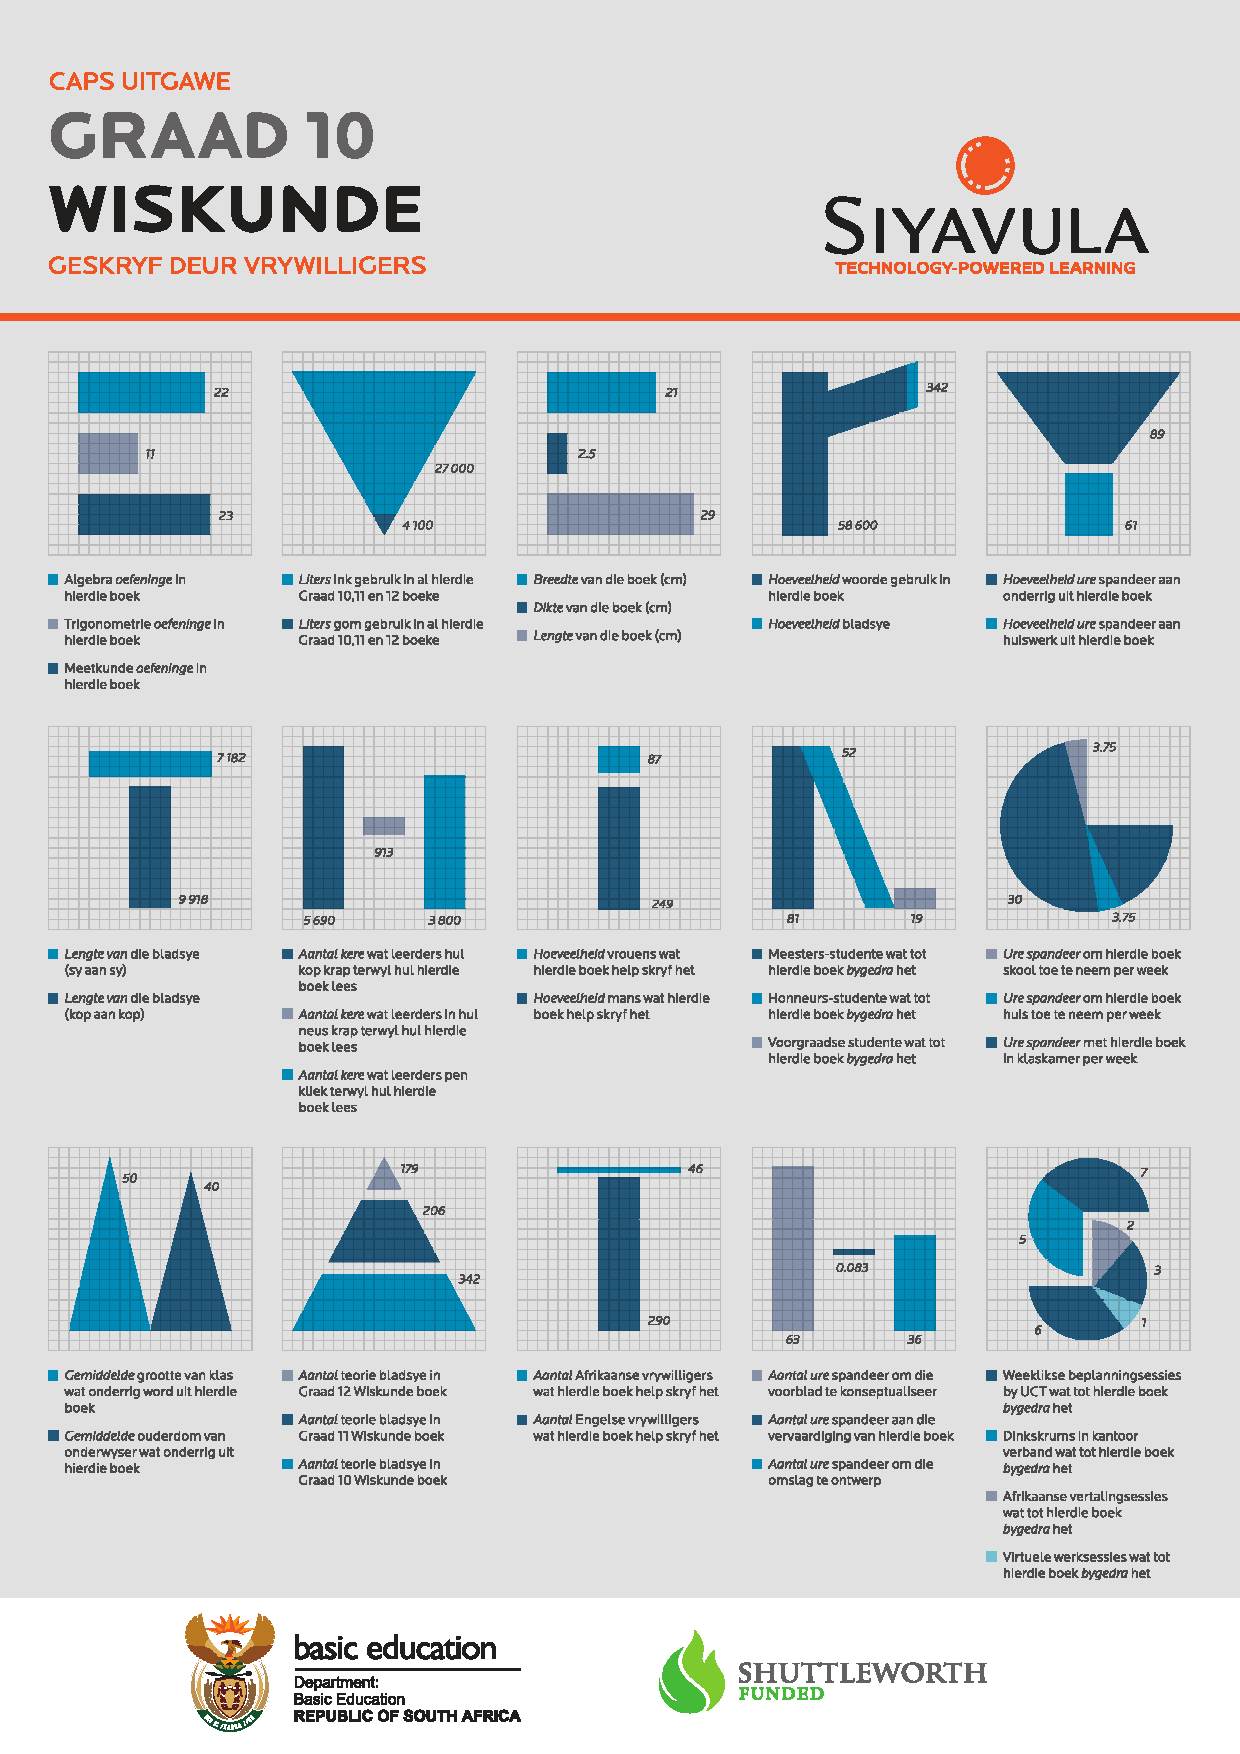
\includepdf[pages=1]{../covers/maths_gr10_afr_front.pdf}
% \newgeometry{paper=a4paper, lmargin=0.1\paperwidth, rmargin=0.1\paperwidth, tmargin=1in, bmargin=1in}

\begin{titlepage}
\begin{adjustwidth}{1in}{1in}
\begin{center}
    \thispagestyle{empty}

    \vspace*{4in}

    {\normalfont\sffamily\fontsize{36}\normalfont\itshape{Everything Maths } \\ \vspace*{1cm}
    {\normalfont\sffamily\fontsize{22}\normalfont\itshape{Grade 10 Mathematics}}
    \vspace*{1in} \\
    \LARGE Version 1 -- CAPS \\

   {\vspace*{2in}
     by Siyavula and volunteers 
  

\vfill

    }}
\end{center}
\end{adjustwidth}
\end{titlepage}






% Copyright notice
\newpage
\thispagestyle{empty}
{
\begin{center}
\normalfont\sffamily\fontsize{22}\normalfont\itshape Copyright notice\\

\vspace*{1in}

\textbf{Your freedom to legally copy this book}\\

\end{center}
}

{\LARGE
You are allowed and encouraged to freely copy this book. You can photocopy, print and distribute it as
often as you like. You can download it onto your mobile phone, iPad, PC or flash drive. You can burn it
to CD, e-mail it around or upload it to your website. \par

The only restriction is that you have to keep this book, its cover and short-codes unchanged.\par

For more information about the Creative Commons Attribution-NoDerivs 3.0 Unported (CC BY-ND
3.0) license see http://creativecommons.org/licenses/by-nd/3.0/}\\

\vspace*{4in}

\begin{center}
\begin{minipage}{0.6\textwidth}

\includegraphics[width=0.8\textwidth]{title_images/cc2.png}
\end{minipage}
\begin{minipage}{0.3\textwidth}

\includegraphics[width=0.8\textwidth]{title_images/cc1.png}
\end{minipage}
\end{center}







% Authors
\newpage
\thispagestyle{empty}


\begin{flushleft} \textbf{\huge Authors List} \end{flushleft}

{\LARGE This book is based upon the original Free High School Science Text which was entirely written by
volunteer academics, educators and industry professionals. Their vision was to see a curriculum aligned
set of mathematics and physical science textbooks which are freely available to anybody and exist
under an open copyright license.} \par

\textbf{\LARGE Siyavula core team} \\

Neels van der Westhuizen; Alison Jenkin; Marina van Zyl; Helen Robertson; Carl Scheffler; Nicola du Toit; Gumani Mudau; Thomas Masango \par

\textbf{\LARGE Original Free High School Science Texts core team}\\

Mark Horner; Samuel Halliday; Sarah Blyth; Rory Adams; Spencer Wheaton \par 


\textbf{\LARGE Original Free High School Science Texts editors}\\

Jaynie Padayachee; Joanne Boulle; Diana Mulcahy; Annette Nell; René Toerien; Donovan Whitfield \par

\textbf{\LARGE Siyavula and Free High School Science Texts contributors}\\

Sarah Abel; Dr. Rory Adams; Andrea Africa; Matthew Amundsen; Ben Anhalt; Prashant Arora; Amos Baloyi; Bongani
Baloyi; Raymond Barbour; Richard Baxter; Tara Beckerling; Dr. Sarah Blyth; Sebastian Bodenstein; Martin Bongers;
Gareth Boxall; Stephan Brandt; Hannes Breytenbach; Wilbur Britz; Graeme Broster; Craig Brown; Richard Burge;
Bianca Böhmer; George Calder-Potts; Eleanor Cameron; Richard Case; Sithembile Cele; Richard Cheng; Fanny
Cherblanc; Dr. Christine Chung; Brett Cocks; Stefaan Conradie; Rocco Coppejans; Tim Craib; Andrew Craig; Tim
Crombie; Dan Crytser; Dr. Anne Dabrowski; Laura Daniels; Jennifer de Beyer; Deanne de Bude; Mia de Vos; Sean
Dobbs; Buhle Donga; William Donkin; Esmi Dreyer; Nicola du Toit; Matthew Duddy; Fernando Durrell; Dr. Dan
Dwyer; Alex Ellis; Tom Ellis; Andrew Fisher; Giovanni Franzoni; Nina Gitau Muchunu; Lindsay Glesener; Kevin
Godby; Dr. Vanessa Godfrey; Terence Goldberg; Dr. Johan Gonzalez; Hemant Gopal; Dr. Stephanie Gould; Umeshree
Govender; Heather Gray; Lynn Greeff; Carine Grobbelaar; Dr. Tom Gutierrez; Brooke Haag; Kate Hadley; Alex Hall;
Dr. Sam Halliday; Asheena Hanuman; Dr. Nicholas Harrison; Neil Hart; Nicholas Hatcher; Jason Hayden; Laura
Hayward; Cho Hee Shrader; Dr. Fritha Hennessy; Shaun Hewitson; Millie Hilgart; Grant Hillebrand; Chris Holdsworth;
Dr. Benne Holwerda; Dr. Mark Horner; Robert Hovden; Mfandaidza Hove; Jennifer Hsieh; Laura Huss; Dr. Matina J.
Rassias; Rowan Jelley; Grant Jelley; Clare Johnson; Luke Jordan; Tana Joseph; Dr. Fabian Jutz; Brian Kamanzi; Dr.
Lutz Kampmann; Simon Katende; Natalia Kavalenia; Paul Kim; Dr. Jennifer Klay; Lara Kruger; Sihle Kubheka;
Andrew Kubik; Dr. Jannie Leach; Nkoana Lebaka; Dr. Tom Leinster; Henry Liu; Christopher Loetscher; Amandla
Mabona; Malothe Mabutho; Stuart Macdonald; Dr. Anton Machacek; Tshepo Madisha; Batsirai Magunje; Dr. Komal
Maheshwari; Michael Malahe; Masoabi Malunga; Masilo Mapaila; Bryony Martin; Nicole Masureik; John Mathew; Dr.
Will Matthews; JoEllen McBride; Dr Melanie Dymond Harper; Nikolai Meures; Riana Meyer; Filippo Miatto; Jenny
Miller; Abdul Mirza; Mapholo Modise; Carla Moerdyk; Tshwarelo Mohlala; Relebohile Molaoa; Marasi Monyau;
Asogan Moodaly; Jothi Moodley; Robert Moon; Calvin Moore; Bhavani Morarjee; Kholofelo Moyaba; Emmanuel
Musonza; Tom Mutabazi; David Myburgh; Kamie Naidu; Nolene Naidu; Gokul Nair; Bridget Nash; Tyrone Negus;
Buntu Ngcebetsha; Thomas O’Donnell; Dr. Markus Oldenburg; Dr. William P. Heal; Dr. Jaynie Padayachee; Poveshen
Padayachee; Masimba Paradza; Dave Pawson; Justin Pead; Nicolette Pekeur; Sirika Pillay; Jacques Plaut; Barry
Povey; Andrea Prinsloo; Joseph Raimondo; Sanya Rajani; Alastair Ramlakan; Dr. Jocelyn Read; Jonathan Reader; Dr.
Matthew Reece; Razvan Remsing; Laura Richter; Max Richter; Sean Riddle; Dr. David Roberts; Christopher Roberts;
Evan Robinson; Raoul Rontsch; Dr. Andrew Rose; Katie Ross; Jeanne-Marié Roux; Mark Roux; Bianca Ruddy; Katie
Russell; Steven Sam; Nathaniel Schwartz; Duncan Scott; Helen Seals; Relebohile Sefako; Prof. Sergey Rakityansky;
Paul Shangase; Cameron Sharp; Ian Sherratt; Dr. James Short; Roger Sieloff; Brandon Sim; Clare Slotow; Bradley
Smith; Greg Solomon; Nicholas Spaull; Dr. Andrew Stacey; Dr. Jim Stasheff; Mike Stay; Mike Stringer; Masixole
Swartbooi; Tim Teatro; Ben Thompson; Shen Tian; Xolani Timbile; Robert Torregrosa; Jimmy Tseng; Tim van Beek;
Neels van der Westhuizen; Frans van Eeden; Pierre van Heerden; Dr. Marco van Leeuwen; Pieter Vergeer; Rizmari
Versfeld; Mpilonhle Vilakazi; Ingrid von Glehn; Tamara von Glehn; Kosma von Maltitz; Helen Waugh; Leandra Webb;
Dr. Dawn Webber; Michelle Wen; Dr. Alexander Wetzler; Dr. Spencer Wheaton; Vivian White; Dr. Gerald Wigger;
Harry Wiggins; Heather Williams; Wendy Williams; Julie Wilson; Timothy Wilson; Andrew Wood; Emma Wormauld;
Dr. Sahal Yacoob; Jean Youssef; Ewald Zietsman








% Everything Maths page
\newpage
\thispagestyle{empty}

{\normalfont\sffamily\fontsize{22}\normalfont\itshape Everything Maths} \par

{ \Large
Mathematics is commonly thought of as being about numbers but mathematics is actually a language! Mathematics is the language that nature speaks to us in. As we learn to understand and speak this language, we can discover many of nature’s secrets. Just as understanding someone’s language is necessary to learn more about them, mathematics is required to learn about all aspects of the world -- whether it is physical sciences, life sciences or even finance and economics.\par


The great writers and poets of the world have the ability to draw on words and put them together in
ways that can tell beautiful or inspiring stories. In a similar way, one can draw on mathematics to
explain and create new things. Many of the modern technologies that have enriched our lives are
greatly dependent on mathematics. DVDs, Google searches, bank cards with PIN numbers are just
some examples. And just as words were not created specifically to tell a story but their existence enabled
stories to be told, so the mathematics used to create these technologies was not developed for its own sake,
but was available to be drawn on when the time for its application was right.\par


There is in fact not an area of life that is not affected by mathematics. Many of the most sought after
careers depend on the use of mathematics. Civil engineers use mathematics to determine how to best
design new structures; economists use mathematics to describe and predict how the economy will react
to certain changes; investors use mathematics to price certain types of shares or calculate how risky
particular investments are; software developers use mathematics for many of the algorithms (such as
Google searches and data security) that make programmes useful.\par



But, even in our daily lives mathematics is everywhere – in our use of distance, time and money.
Mathematics is even present in art, design and music as it informs proportions and musical tones. The
greater our ability to understand mathematics, the greater our ability to appreciate beauty and
everything in nature. Far from being just a cold and abstract discipline, mathematics
embodies logic, symmetry, harmony and technological progress. More than any other language,
mathematics is everywhere and universal in its application.\par


See introductory video by Dr. Mark Horner: \raisebox{-0.2em}{
\includegraphics[height=1em]{../icons/video.pdf}} \textbf{short-code} at www.everythingmaths.co.za



}





% Webbook page

\newpage
\thispagestyle{empty}

{\normalfont\sffamily\fontsize{22}\normalfont\itshape More than a regular textbook} \par

\begin{center}
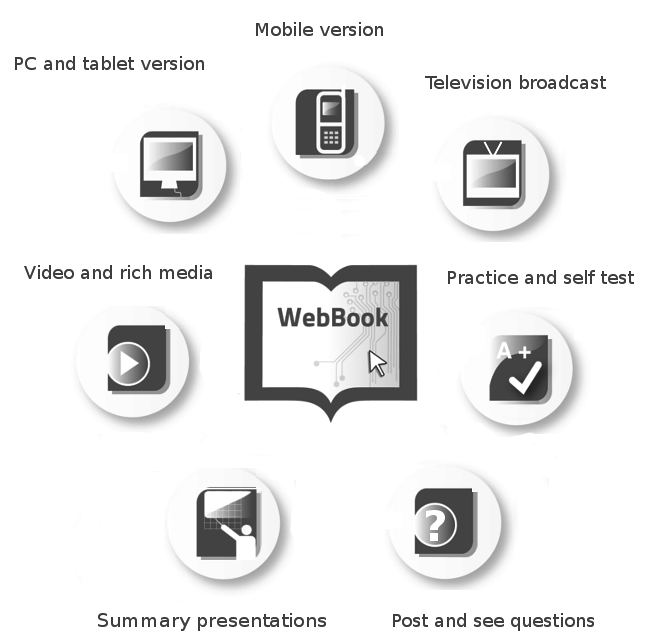
\includegraphics[width=0.70\textwidth]{title_images/morethantextbook.png}
\end{center}

\par
{\Large
\textbf{\textit{Everything Science}} is not just a Science textbook. It has everything you expect from
your regular printed school textbook, but comes with a whole lot more. For a start, you can download or read it
on-line on your mobile phone, computer or iPad, which means you have the convenience of accessing
it wherever you are.\par


We know that some things are hard to explain in words. That is why every chapter comes with video
lessons and explanations which help bring the ideas and concepts to life. Summary presentations at
the end of every chapter offer an overview of the content covered, with key points highlighted for easy
revision.\par


All the exercises inside the book link to a service where you can get more practice, see the full solution
or test your skills level on mobile and PC.\par


We are interested in what you think, wonder about or struggle with as you read through the book and
attempt the exercises. That is why we made it possible for you to use your mobile phone or computer to
digitally pin your question to a page and see what questions and answers other readers pinned up.\par


This book is the same one used by Mindset Learn in their new television broadcast, where experienced educators work through it, explain the concepts and work out exercises from the book.
}




% mobile or PC
\newpage
\thispagestyle{empty}

{\normalfont\sffamily\fontsize{22}\normalfont\itshape Everything Science on your mobile or PC} \par

{\Large
You can have this textbook at hand wherever you are – whether at home, on the the train or at school.
Just browse to the on-line version of Everything Science on your mobile phone, tablet or computer. To
read it off-line you can download a PDF or e-book version.\par


To read or download it, go to \textbf{www.everythingscience.co.za} on your phone or computer.} \vspace*{2cm}


\begin{center}
\begin{minipage}{0.4\textwidth}
\centering
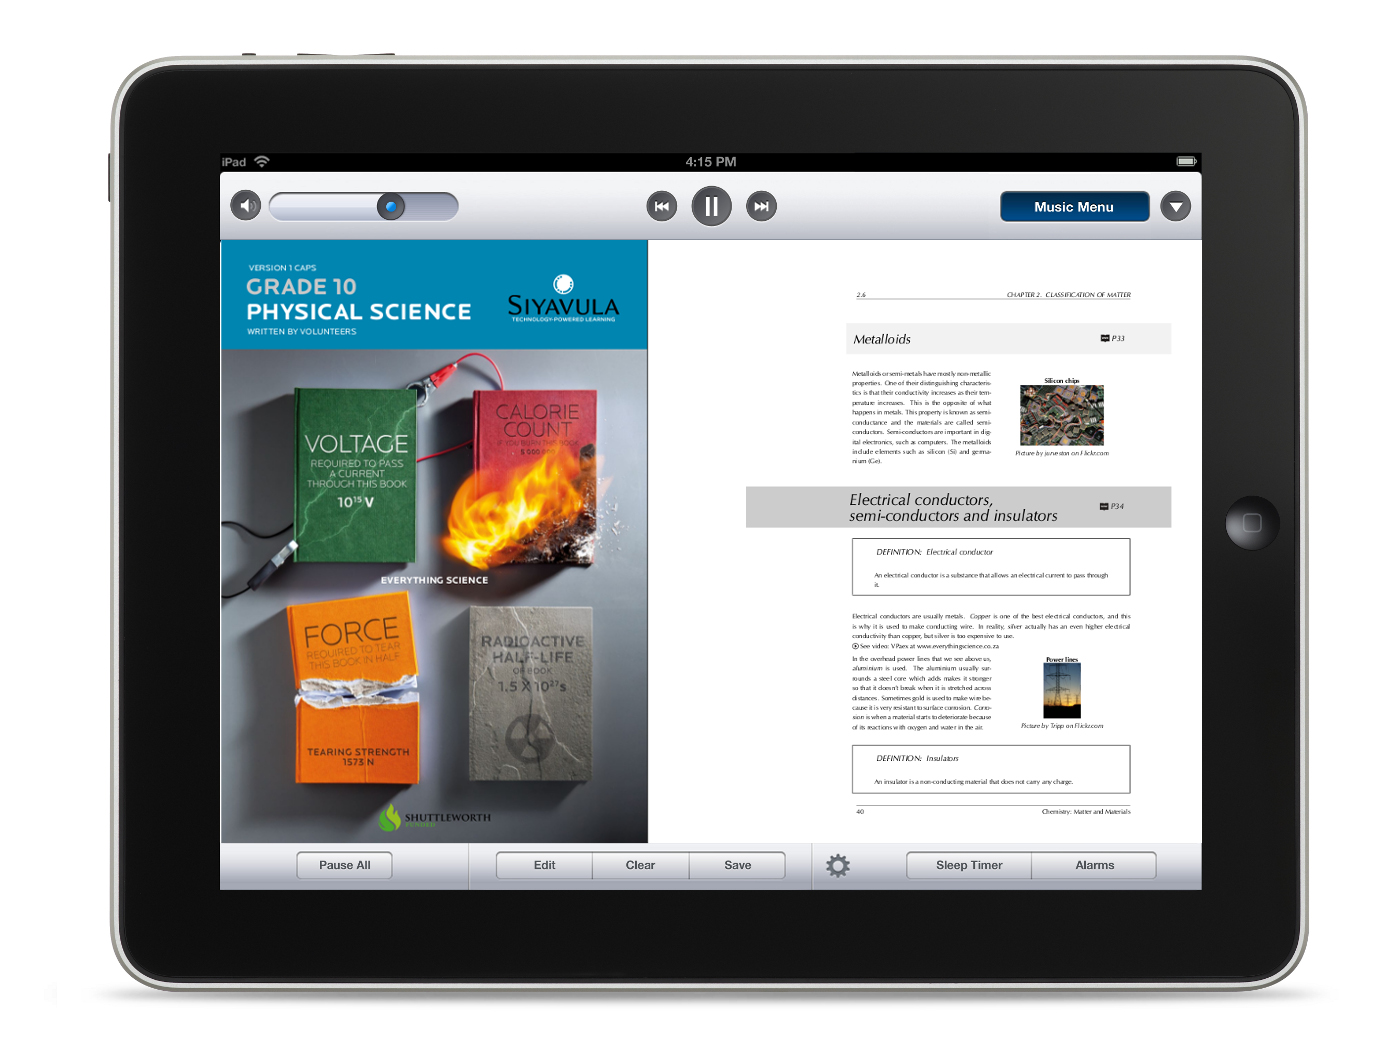
\includegraphics[width=0.8\textwidth]{title_images/ipad.jpg}
\end{minipage}
\begin{minipage}{0.4\textwidth}
\centering

\includegraphics[width=0.4\textwidth]{title_images/phone.png}
\end{minipage}
\end{center}

\vspace*{2cm}


{\normalfont\sffamily\fontsize{22}\normalfont\itshape Using the icons and short-codes} \par

{\Large
Inside the book you will find these icons to help you spot where videos, presentations, practice tools
and more help exist. The short-codes next to the icons allow you to navigate directly to the resources
on-line without having to search for them.\par


\begin{tabular}{lcl}
\raisebox{-0.8em}{
\includegraphics[width=0.8cm]{../icons/www.pdf}} & (A123) & Go directly to a section \\
\raisebox{-0.8em}{
\includegraphics[width=0.8cm]{../icons/video.pdf}} & (V123) & Video, simulation or presentation \\
\raisebox{-0.8em}{
\includegraphics[width=0.8cm]{../icons/aplus.pdf}} & (P123) & Practice and test your skills \\
\raisebox{-0.8em}{
\includegraphics[width=0.8cm]{../icons/help.pdf}} & (Q123) & Ask for help or find an answer \\
\end{tabular}
\par
\vspace*{1cm}

To watch the videos on-line, practise your skills or post a question, go to the \textit{Everything Science} website at \textbf{www.everythingscience.co.za} on your mobile or PC and enter the short-code in the navigation box.
}




% video lessons
\newpage
\thispagestyle{empty}

{\normalfont\sffamily\fontsize{22}\normalfont\itshape Video lessons} \par

{\Large

Look out for the video icons inside the book. These will take you to video lessons created by \textit{Mindset
Learn} that help bring the ideas and concepts on the page to life. Get extra insight, detailed
explanations and worked examples. See the concepts in action and hear real people talk about how they
use maths and science in their work. \par

\begin{center}
\caption{See video explanation \raisebox{-0.6em}{
\includegraphics[width=0.7cm]{../icons/video.pdf}} (Video: V123)}\\
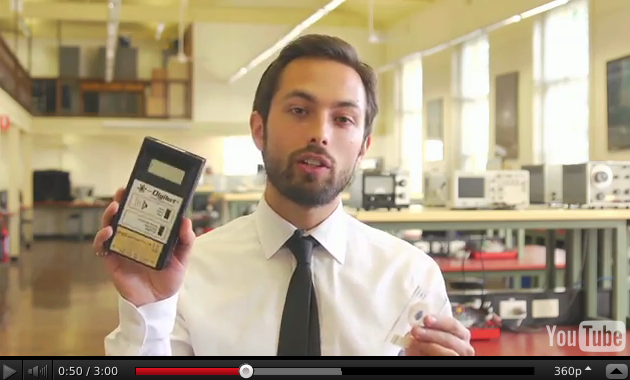
\includegraphics[width=0.5\textwidth]{title_images/veritasiumvideo.png}
\end{center}\par

}
\vspace{0.5cm}
{\normalfont\sffamily\fontsize{22}\normalfont\itshape Video exercises} \par

{\Large

Wherever there are exercises in the book you will see icons and short-codes for video solutions,
practice and help. These short-codes will take you to video solutions of select exercises to show you
step-by-step how to solve such problems. \par

\begin{center}
\caption{See video exercise \raisebox{-0.6em}{
\includegraphics[width=0.7cm]{../icons/video.pdf}} (Video: V123)} \\
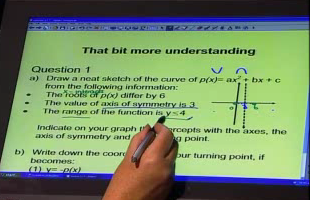
\includegraphics[width=0.5\textwidth]{title_images/mindsetexercise.png}
\end{center}
\par
You can get these videos by:
\begin{itemize}
    \item viewing them on-line on your mobile or computer
    \item downloading the videos for off-line viewing on your phone or computer
    \item ordering a DVD to play on your TV or computer
    \item downloading them off-line over Bluetooth or Wi-Fi from select outlets
\end{itemize}
}


% practise and test your skills
\newpage
\thispagestyle{empty}
{\Large

To view, download, or for more information, visit the Everything Science website on your phone or
computer at \underline{www.everythingscience.co.za}  \par
\vspace*{1cm}
{\normalfont\sffamily\fontsize{22}\normalfont\itshape Practice and test your skills} \par


One of the best ways to prepare for your tests and exams is to practice answering the same kind of
questions you will be tested on. At every set of exercises you will see a practice icon and short-code.
This on-line practice for \textbf{mobile} and \textbf{PC} will keep track of your performance and progress, give you
feedback on areas which require more attention and suggest which sections or videos to look at.

\begin{center}
\caption{See more practice \raisebox{-0.6em}{
\includegraphics[width=0.7cm]{../icons/aplus.pdf}} (QM123)} \\
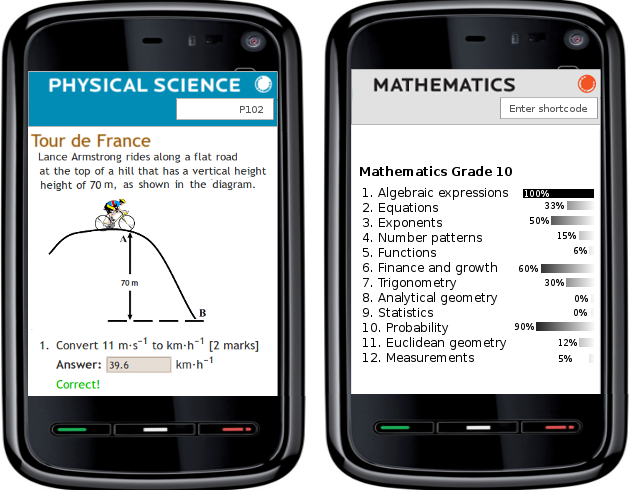
\includegraphics[width=0.65\textwidth]{title_images/practicephones.png}
\end{center}
\par



To practice and test your skills:\par

Go to \underline{www.everythingscience.co.za} on your mobile phone or PC and enter the short-code.\par

\vspace*{1cm}


{\normalfont\sffamily\fontsize{22}\normalfont\itshape Television broadcasts} \par
This book is the same one used by \textbf{Mindset Learn} in their television broadcast where experienced
educators explain the key concepts, perform live experiments and work out exercises from the book.
\textbf{Mindset Learn} broadcasts a full 28 hours of curriculum support each week of term. \par


Maths can be seen on Mondays and Science on Tuesdays. There is also Life Sciences on Wednesdays
and Maths Literacy on Thursdays. Revision of the week's work is done on Saturdays for Grade 12 and on
Sundays for Grades 10 and 11.


}




% practise and test your skills
\newpage
\thispagestyle{empty}
{\Large

\begin{table*}[h]
\large
\begin{tabular}{lll}
\textbf{Maths and Science Broadcasts}&&\\
Grade 10  Maths & Mondays at 4pm & Every second Sunday at 1pm\\
Grade 11  Maths & Mondays at 5pm & Every second Sunday at 9am\\
Grade 12  Maths & Mondays at 6pm & Every Saturday at 9am\\
Grade 10  Science & Tuesdays at 4pm & Every second Sunday at 1pm\\
Grade 11  Science & Tuesdays at 5pm & Every second Sunday at 9am\\
Grade 12  Science & Tuesdays at 6pm & Every Saturday at 11am\\
\textbf{Other broadcasts} & & \\
Grade 10  Life Science & Wednesdays at 4pm & Every second Sunday at 3pm\\
Grade 11  Life Science & Wednesdays at 5pm & Every second Sunday at 9am\\
Grade 12  Life Science & Wednesdays at 6pm & Every Saturday at 1pm\\
Grade 10  Maths Literacy & Thursdays at 4pm & Every second Sunday at 3pm\\
Grade 11  Maths Literacy & Thursdays at 5pm & Every second Sunday at 9am\\
Grade 12  Maths Literacy & Thursdays at 6pm & Every Saturday at 3pm\\
\end{tabular}
\end{table*}


\textbf{You can watch these live sessions on:}
\begin{itemize}
    \item Mindset free-to-air for schools (ask your school)
    \item Channels 319 on DStv
    \item Toptv on 319 on TopTV
\end{itemize}


}

% Put the margins back for the rest of the book

\newgeometry{lmargin=0.1\paperwidth, rmargin=0.25\paperwidth, tmargin=1in, bmargin=1in, twoside, centering, includehead,  marginparwidth=0.225\paperwidth}

\normalfont
 

\tableofcontents
\mainmatter

\renewcommand{\sectionmark}[1]{\markright{\thesection}{}}
\renewcommand{\footrulewidth}{0.4pt}

\newpage

    % chapter includes

% 
% \chapter{Algebraic expressions}
\fancyfoot[LO,RE]{Focus Area: Mathematics}
\section{Rational and irrational numbers}
\setcounter{figure}{1}
\setcounter{subfigure}{1}

A number is a way of representing quantity. The numbers used in high school are all real numbers, but there are many different ways of writing any single real number.\par 
This section describes rational and irrational numbers.\par 
\chapterstartvideo{VMabo}
% \setcounter{subfigure}{0}
% \begin{figure}[H] % horizontal\label{m38348*circuits-1}
% \textnormal{Khan Academy video on Integers and Rational Numbers}\vspace{.1in} \nopagebreak
% \label{m38348*yt-media1}\label{m38348*yt-video1}
% \raisebox{-5 pt}{ 
\includegraphics[width=0.5cm]{col11306.imgs/summary_www.png}} { (Video:  MG10034 )}
% \vspace{2pt}
% \vspace{.1in}
% \end{figure}       

\par 
\subsection*{The big picture of numbers}
\addcontentsline{toc}{subsection}{The big picture of numbers}


\setcounter{subfigure}{0}
\begin{figure}[H] % horizontal\label{m38348*id62548}
\begin{center}
% \label{m38348*id62548!!!underscore!!!media}\label{m38348*id62548!!!underscore!!!printimage}
%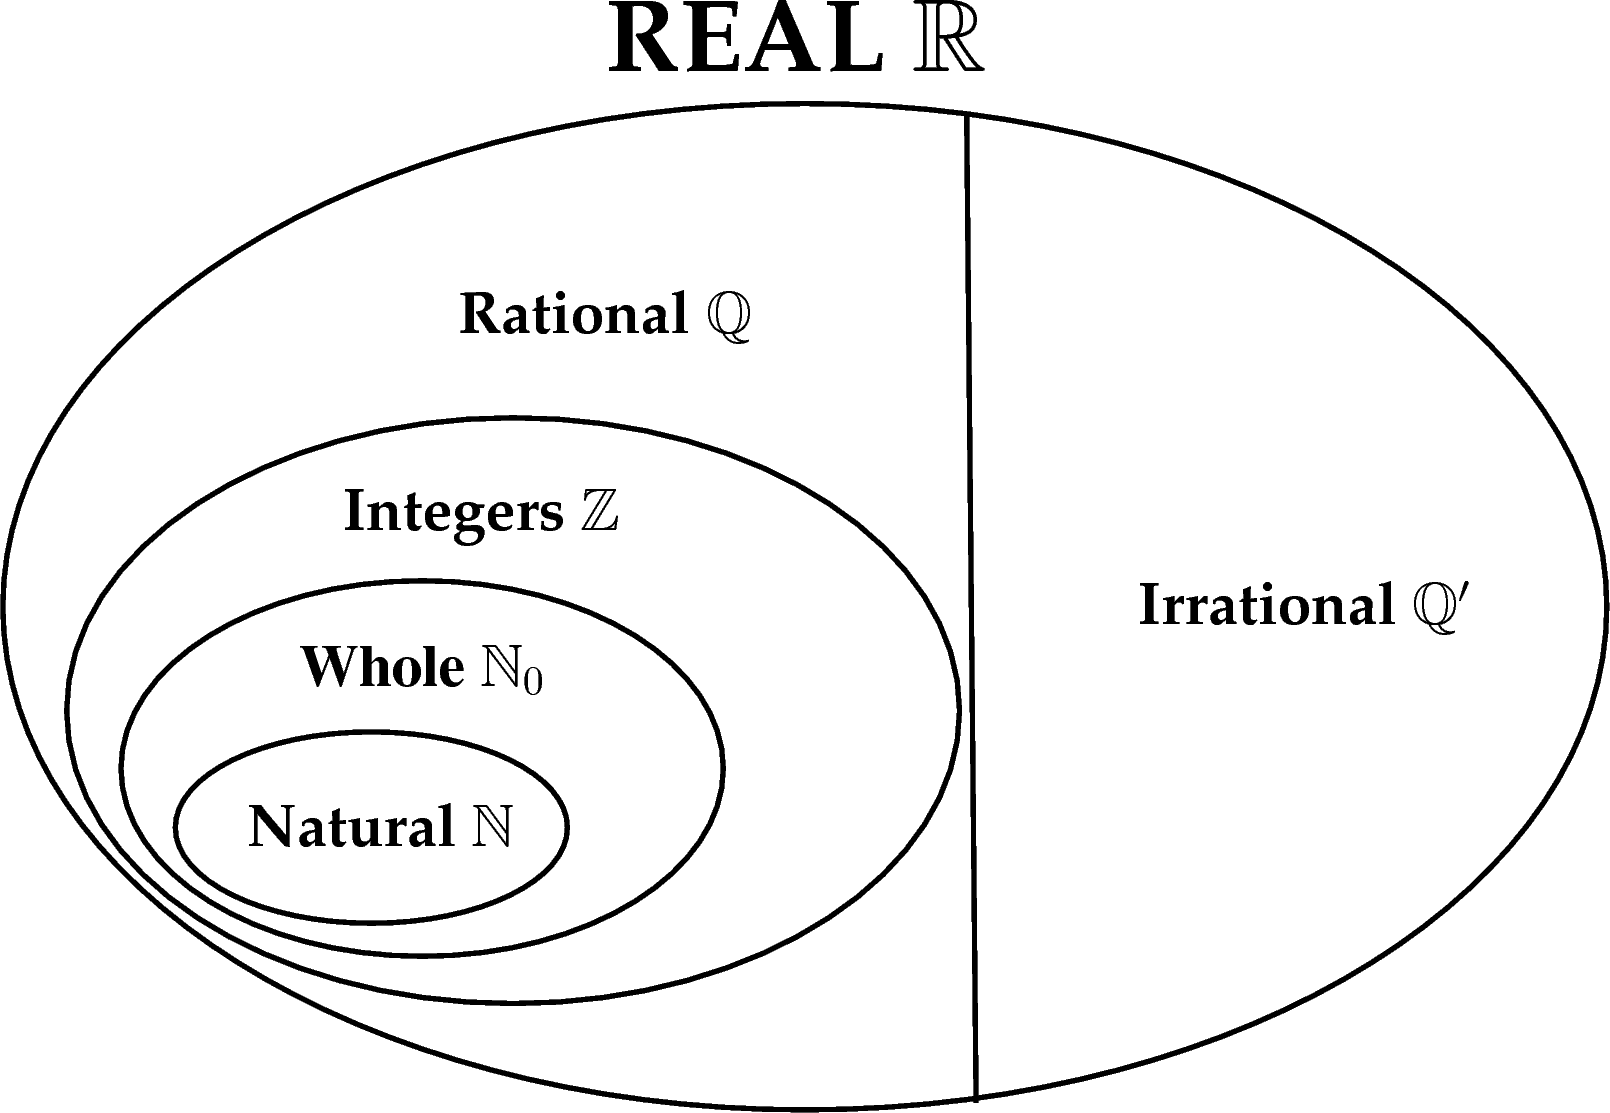
\includegraphics[width=9cm]{col11306.imgs/m38348_MG10C3_001.png} % m38348;MG10C3\_001.png;;;6.0;8.5;
\scalebox{0.6} % Change this value to rescale the drawing.
{
\begin{pspicture}(0,-4.764375)(14.481563,4.804375)
\psellipse[linewidth=0.04,dimen=outer](6.81,-0.484375)(6.81,4.28)
\psline[linewidth=0.04cm](8.18,3.695625)(8.26,-4.684375)
\psellipse[linewidth=0.04,dimen=outer](4.34,-1.364375)(3.8,2.5)
\psellipse[linewidth=0.04,dimen=outer](3.57,-1.854375)(2.57,1.61)
% \usefont{T1}{ppl}{b}{n}
\rput(6.735781,4.350625){\Huge REAL $\mathbb{R}$}
% \usefont{T1}{ppl}{b}{n}
\rput(11.03875,-0.484375){\Huge Irrational $\mathbb{Q'}$}
% \usefont{T1}{ppl}{b}{n}
\rput(5.11875,1.975625){\Huge Rational $\mathbb{Q}$}
% \usefont{T1}{ppl}{b}{n}
\rput(4.06875,0.275625){\Huge Integers $\mathbb{Z}$}
% \usefont{T1}{ppl}{b}{n}
\rput(3.21875,-2.324375){\Huge Natural $\mathbb{N}$}
\psellipse[linewidth=0.04,dimen=outer](3.14,-2.354375)(1.68,0.83)
% \usefont{T1}{ptm}{b}{n}
\rput(3.5735939,-1.024375){\Huge Whole $\mathbb{N}_0$}
\end{pspicture} 
}
\vspace{2pt}
\vspace{.1in}
\end{center}
\end{figure}       
\par 
We use the following definitions:\par 
\begin{itemize}[itemsep=5pt]
\item natural numbers are $\{1; 2; 3; \ldots\}$
\item whole numbers are $\{0; 1; 2; 3; \ldots\}$
\item integers are $\{\ldots -3; -2; -1; 0; 1; 2; 3; \ldots\}$
\end{itemize}



\Definition{Rational number}{
A rational number is any number which can be written as: 
%       \label{m38348*uid6}\nopagebreak\noindent{}

\begin{equation*}
\frac{a}{b}
\end{equation*}
where $a$ and $b$ are integers and $b\ne 0$. \par 
} 


The following numbers are all rational numbers:\par 


\begin{equation*}
\frac{10}{1};\frac{21}{7};\frac{-1}{-3};\frac{10}{20};\frac{-3}{6}
\end{equation*}
We see that all numerators and all denominators are integers.\par 

\par
This means that all integers are rational numbers, because they can be written with a denominator of $1$.\par 
Consider

\begin{equation*}
\frac{\sqrt{2}}{7} ; \frac{20}{\pi}
\end{equation*}
These are not rational numbers, because either the numerator or the denominator is not an integer.\par 
A number may not be written as an integer divided by another integer, but may still
be a rational number. The rule is, if a number can be written
as a fraction of integers, it is rational even if it can be written in other
ways as well. These two examples might not look like rational numbers
at first glance, but because there have equivalent forms that can be expressed as an
integer divided by another integer, they are rational:\par 
\nopagebreak\noindent{}
\begin{equation*}    
\frac{-1,33}{-3}=\frac{133}{300}; ~~~~~~\frac{-3}{6,39}=\frac{-300}{639}=\frac{-100}{213}
\end{equation*}


\subsection*{Decimal numbers}
\addcontentsline{toc}{subsection}{Decimal numbers}
\nopagebreak
All integers and fractions with integer numerators and denominators are rational numbers. There are two more forms of rational numbers.\par 




\begin{activity}{Decimal numbers }
\nopagebreak
You can write the rational number
$\frac{1}{2}$ as the decimal number $0,5$. Write the following numbers as
decimals:\par 
\begin{enumerate}[itemsep=5pt, label=\textbf{\arabic*}. ] 
\item $\dfrac{1}{4}$
\item $\dfrac{1}{10}$
\item $\dfrac{2}{5}$
\item $\dfrac{1}{100}$
\item $\dfrac{2}{3}$
\end{enumerate}
Do the numbers after the decimal comma end or do they continue? If they continue, is there a recurring pattern to the numbers? \par 
\end{activity}

You can write any rational number as a decimal number but not all decimal numbers are rational numbers. However, two types of decimal numbers can be written as rational numbers:\par 
\begin{itemize}
\item decimal numbers that end or terminate, for example the fraction $\dfrac{4}{10}$ can be written as $0,4$.
\item decimal numbers that have a recurring pattern of a single digit, for example the fraction $\dfrac{1}{3}$ can be written as 
$0,\dot{3}$. 
The dot represents recurring $3$'s i.e.
$0,333\ldots=0,\dot{3}$.
\item decimal numbers that have a recurring pattern of a single digit, for example the fraction $\dfrac{2}{3}$ can also be written as 
$0,\bar{6}$. 
The bar represents recurring $6$'s i.e.
$0,666\ldots=0,\bar{6}$.
\item decimal numbers that have a recurring pattern of multiple digits, for example the fraction $\dfrac{2}{11}$ can also be written as 
$0,\overline{18}$. 
The bar represents a recurring pattern of $1$ and $8$'s i.e.
$0,181818\ldots=0,\overline{18}$.
\end{itemize}


\Tip{You can use a dot or a bar over the repeated numbers to indicate that the decimal is a recurring decimal. If the bar covers more than one number, then all numbers beneath the bar are recurring.}



\subsection{Converting terminating decimals into rational numbers}

% \addcontentsline{toc}{subsection}{Converting terminating decimals into rational numbers}
A decimal number has an integer part and a fractional part. For example, $10,589$ has an integer part of $10$ and a fractional part of $0,589$ because $10+0,589=10,589$. The fractional part can be written as a rational number i.e. with a numerator and denominator that are integers. \\
\\
Each digit after the decimal point is a fraction with a denominator in increasing powers of $10$. For example 
\begin{itemize}
 \item $0,1$ is $\dfrac{1}{10}$
\item $0,01$ is $\dfrac{1}{100}$
\item $0,001$ is $\dfrac{1}{1000}$
\end{itemize}

This means that
\begin{equation*}
 \begin{array}{lll}10,589& = &10 + \dfrac{5}{10} + \dfrac{8}{100} + \dfrac{9}{1000} &\\ 
  &=& 10 \dfrac{589}{1000} \\
\\
&=& \dfrac{10589}{1000}
 \end{array}

\end{equation*}

\subsection{Converting recurring decimals into rational numbers}


When the decimal is a recurring decimal, a bit more work is needed to write the fractional part of the decimal number as a fraction.\par 

\begin{wex}
{%title
Converting decimal numbers to fractions
}
{%question
Write $0,\dot{3}$ in the form $\dfrac{a}{b}$ (where $a$ and $b$ are integers).
}
{%answer

\westep{Define an equation}
Let $x = 0,33333\ldots$


\westep{Multiply by $10$ on both sides}

$10x = 3,33333\ldots$


\westep{Subtract the first equation from the second equation}

$9x = 3 $

\westep{Simplify}

$ x = \dfrac{3}{9} = \dfrac{1}{3} $
}
\end{wex}


\begin{wex}
{%title
Converting decimal numbers to fractions
}
{%question
\\Write $5,\dot{4}\dot{3}\dot{2}$ as a rational fraction.
}
{%answer

\westep{Define an equation}

$$ x = 5,432432432\ldots $$

\westep{Multiply by $1000$ on both sides}

$$ 1000x = 5432,432432432\ldots $$

\westep{Subtract the first equation from the second equation}

$$ 999x = 5427 $$

\westep{Simplify}

$$ x = \dfrac{5427}{999} = \dfrac{201}{37} $$

}
\end{wex}




For the first example, the decimal was multiplied by $10$ and for the second example, the decimal was multiplied by $1000$. This is because for the first example there was only one digit (i.e. $3$) recurring, while for the second example there were three digits (i.e. $432$) recurring.\par 
In general, if you have one digit recurring, then multiply by $10$. If you have two digits recurring, then multiply by $100$. If you have three digits recurring, then multiply by $1000$ and so on.\par

Not all decimal numbers can be written as rational numbers. Why? Irrational decimal numbers like 
$\sqrt{2}=1,4142135\ldots$
cannot be written with an integer numerator and denominator, because they do not have a pattern of recurring digits and they do not terminate. However, when possible, you should try to use rational numbers or fractions instead of decimals.
% \label{m38348*secfhsst!!!underscore!!!id606}




\section{Irrational numbers}
\setcounter{figure}{1}
\setcounter{subfigure}{1}


We have seen that recurring decimals may take a lot of paper and ink to write out. Writing numbers to many decimal places or a high accuracy is very inconvenient and rarely gives practical answers. For this reason we often estimate the number to a certain number of decimal places or to a given number of significant figures, which is even better.\par 

\Definition{Irrational numbers}{Irrational numbers are numbers that cannot be written as a fraction with the numerator and denominator as integers. This means that any number that is not a terminating or recurring decimal number is irrational. 
}

Examples of irrational numbers:\par 

\begin{equation*}
\sqrt{2};~\sqrt{3};~\sqrt[3]{4};~\pi ;
~\frac{1+\sqrt{5}}{2}\approx 1,618
\end{equation*}




\Tip{When irrational numbers are written in decimal form, they go on forever and
there is no repeated pattern of digits. \\The square roots of non-perfect squares and the cube roots of non-perfect cubes are all irrational.}

If you are asked to identify whether a number is rational or irrational, first write the number in decimal form. If the number terminates then it is rational. If it goes on forever, then look for a repeated pattern of digits. If there is no repeated pattern, then the number is irrational.\par 
When you write irrational numbers in decimal form, you may (if you have a lot of time and paper!) continue writing them for many, many decimal places. However, this is not convenient and it is often necessary to round off.\par 



\begin{activity}{Irrational numbers }
\nopagebreak
Which of the following cannot be
written as a rational number?\par \vspace{0.5cm}
\textbf{Remember}: A rational number is a fraction with numerator and denominator as integers. Terminating decimal numbers or recurring decimal numbers are rational.\par 
\begin{enumerate}[itemsep=5pt, label=\textbf{\arabic*}. ] 
\item $\pi =3,14159265358979323846264338327950288419716939937510\ldots$
\item $1,4$
\item $1,618\phantom{\rule{0.166667em}{0ex}}033\phantom{\rule{0.166667em}{0ex}}989\phantom{\rule{0.166667em}{0ex}}\ldots$
\item $100$
\item $1,7373737373\ldots$
\item $0,\overline{02}$
\end{enumerate}
\end{activity}


\begin{exercises}{}{
\begin{enumerate}[itemsep=5pt, label=\textbf{\arabic*}. ] 
\item If $a$ is an integer, $b$ is an integer and $c$ is irrational, which of the following are rational numbers? 
  \begin{enumerate}[itemsep=5pt, label=\textbf{(\alph*)} ] 
    \item $\dfrac{5}{6}$
    \item $\dfrac{a}{3}$
    \item $\dfrac{-2}{b}$
    \item $\dfrac{1}{c}$
    \end{enumerate}
\item If $\dfrac{a}{1}$ is a rational number, which of the following are valid values for $a$?
    \begin{enumerate}[itemsep=5pt, label=\textbf{(\alph*)} ] 
    \item $1$
    \item $-10$
    \item $\sqrt{2}$
    \item $2,1$
    \end{enumerate}
%         \end{enumerate}
% \par \raisebox{-0.2em}{
\includegraphics[height=1em]{../icons/www.pdf}} Find the answers with the shortcodes:
%  \par \begin{tabular}[h]{cccccc}
%  (1.) l35  &  (2.) l3N  & \end{tabular}}
% \end{exercises}
% 
%            \begin{exercises}{Fractions }{
%             \nopagebreak
%       \label{m38348*id63882}\begin{enumerate}[itemsep=5pt, label=\textbf{\arabic*}. ] 
\item Write the following as fractions:
    \begin{enumerate}[itemsep=5pt, label=\textbf{(\alph*)} ] 
    \item $0,1$
    \item $0,12$
    \item $0,58$
    \item $0,2589$
    \end{enumerate}
%         \end{enumerate}
% \par \raisebox{-0.2em}{
\includegraphics[height=1em]{../icons/www.pdf}} Find the answers with the shortcodes:
%  \par \begin{tabular}[h]{cccccc}
%  (1.) l3R  & \end{tabular}}
% \end{exercises}
% 
% \begin{exercises}{Repeated Decimal Notation }{
% %             \nopagebreak
%       \label{m38348*id64513}\begin{enumerate}[itemsep=5pt, label=\textbf{\arabic*}. ] 
\item Write the following using the recurring decimal notation:
    \begin{enumerate}[itemsep=5pt, label=\textbf{(\alph*)} ] 
    \item $0,11111111\ldots$
    \item $0,1212121212\ldots$
    \item $0,123123123123\ldots$
    \item $0,11414541454145\ldots$
    \end{enumerate}
\item Write the following in decimal form, using the recurring decimal notation:
    \begin{enumerate}[itemsep=5pt, label=\textbf{(\alph*)} ] 
    \item $\dfrac{2}{3}$
    \item $1\dfrac{3}{11}$
    \item $4\dfrac{5}{6}$
    \item $2\dfrac{1}{9}$
    \end{enumerate}
\item Write the following decimals in fractional form:
    \begin{enumerate}[itemsep=5pt, label=\textbf{(\alph*)} ] 
    \item $0,\dot{5}$
    \item $0,6\dot{3}$
    \item $5,\overline{31}$
    \end{enumerate}
\end{enumerate}
\practiceinfo 
\par \raisebox{-0.2em}{
\includegraphics[height=1em]{../icons/www.pdf}} Find the answers with the shortcodes:
 \par \begin{tabular}[h]{cccccc}
 (1.) lD1  &  (2.) l3N  &  (3.) l3R  & (4.) l3U & (5.) l3n & (6.) lDr \end{tabular}
}
\end{exercises}

\section{Rounding off}
\nopagebreak
%%$ \hspace{-5pt}\begin{array}{cccccccccccc}   
\includegraphics[width=0.75cm]{col11306.imgs/summary_fullmarks.png} &   \end{array} $ \hspace{2 pt}\raisebox{-5 pt}{} {(section shortcode: MG10057 )} \par 
Rounding off or approximating a decimal number to a given number of decimal places is the quickest way to approximate a number. For example, if you wanted to round off $2,6525272$ to three decimal places, you would first count three places after the decimal and place a $|$ between the third and fourth numbers after the decimal.\par 

\begin{equation*}
2,652|5272
\end{equation*}
All numbers to the right of the $|$ are ignored after you have determined whether the number in the third decimal place must be rounded up or rounded down. You round up the final digit if the first digit after the $|$ was greater than or equal to $5$ and round down (leave the digit unchanged) otherwise. In the case that the first digit before the $|$ is $9$ and you need to round up, then the $9$ becomes a $0$ and the second digit before the $|$ is rounded up.\par 
So, since the first digit after the $|$ is a $5$, we must round up the digit in the third decimal place to a $3$ and the final answer of $2,6525272$ rounded to three decimal places is $2,653$.
\par


\begin{wex}{Rounding off }

{Round off the following numbers to the indicated number of decimal places: 
\begin{enumerate}[itemsep=5pt, label=\textbf{\arabic*}. ] 

\item $\frac{120}{99}=1,212121212\dot{1}\dot{2}$ to $3$ decimal places.
\item $\pi =3,141592654\ldots$ to $4$ decimal places.
\item $\sqrt{3}=1,7320508\ldots$ to $4$ decimal places.
\item $2,78974526\ldots$ to $3$ decimal places.
\end{enumerate}
}
{

\westep{Mark off the required number of decimal places}

\begin{enumerate}[itemsep=5pt, label=\textbf{\arabic*}. ] 
\item $\frac{120}{99}=1,212|121212\dot{1}\dot{2}$
\item $\pi =3,1415|92654\ldots$
\item $\sqrt{3}=1,7320|508\ldots$
\item $2,789|74526\ldots$
\end{enumerate}

\westep{Check the next digit to see if you must round up or round down}
\begin{enumerate}[itemsep=5pt, label=\textbf{\arabic*}. ]
\item The last digit of $\frac{120}{99}=1,212|121212\dot{1}\dot{2}$  must be rounded down.
\item The last digit of $\pi =3,1415|92654\ldots$ must be rounded up.
\item The last digit of $\sqrt{3}=1,7320|508\ldots$ must be rounded up.
\item  The last digit of $2,789|74526\ldots$ must be rounded up .
\newline Since this is a $9$, we replace it with a $0$ and round up the second last digit.
\end{enumerate}

\westep{Write the final answer}
\begin{enumerate}[itemsep=5pt, label=\textbf{\arabic*}. ]
\item $\frac{120}{99}=1,212$ rounded to $3$ decimal places.
\item $\pi =3,1416$  rounded to $4$ decimal places.
\item $\sqrt{3}=1,7321$ rounded to $4$ decimal places.
\item $2,790$
\end{enumerate}
}  
\end{wex}

}

\begin{exercises}{}
{
Use your calculator to write the following in decimal form, round off to $3$ decimal places:
\begin{enumerate}[itemsep=5pt, label=\textbf{\arabic*}. ]
 \item $4\pi$
\item $\sqrt{11}$
\item $\dfrac{0,8}{3}$
\item $\sqrt[3]{7}$
\item $2\sqrt{10}$
\item $\dfrac{1}{18}$
\end{enumerate}
\practiceinfo 
\par \raisebox{-0.2em}{
\includegraphics[height=1em]{../icons/www.pdf}} Find the answers with the shortcodes:
 \par \begin{tabular}[h]{cccccc}
 (1.) lDY  &  (2.) lDY  &  (3.) lDY  & (4.) lDY & (5.) lDY & (6.) lDY \end{tabular}
}

\end{exercises}


\section{Estimating surds}
\setcounter{figure}{1}
\setcounter{subfigure}{1}
If the ${n}^{\mathrm{th}}$ root of a number cannot be simplified to a rational number, we call it a surd. For example, $\sqrt{2}$ and $\sqrt[3]{6}$ are surds, but $\sqrt{4}$ is not a surd because it can be simplified to the rational number $2$.\par 
In this chapter we will look at surds of the form $\sqrt[n]{a}$, where $a$ is any positive number, for example $\sqrt{7}$ or $\sqrt[3]{5}$. It is very common for $n$ to be $2$, so we usually do not write $\sqrt[2]{a}$. Instead we write the surd as just $\sqrt{a}$.\par 
It is sometimes useful to know the approximate value of a surd without having to use a calculator. For example, we want to be able to estimate where a surd like $\sqrt{3}$ is on the number line. From a calculator we know that $\sqrt{3}$ is equal to $1,73205\ldots$. It is easy to see that $\sqrt{3}$ is above $1$ and below $2$. But to see this for other surds like $\sqrt{18}$ without using a calculator, you must first understand the following:\par 


\Identity{}{
\begin{center}
If $a$ and $b$ are positive whole numbers, and $a\lessthan{}b$, then $\sqrt[n]{a}\lessthan{}\sqrt[n]{b}$. 
\end{center}}
\par
       
\Note{A perfect square is the number obtained when an integer is squared. For example $9$ is a perfect square since ${3}^{2}=9$. \\Similarly, a perfect cube is a number which is the cube of an integer. For example $27$ is a perfect cube, because ${3}^{3}=27$.}



Consider the surd $\sqrt[3]{52}$, it lies somewhere between $3$ and $4$, because $\sqrt[3]{27}=3$ and $\sqrt[3]{64}=4$ and $52$ is between $27$ and $64$. Checking on a calculator we see that $\sqrt[3]{52}=3,73\ldots$ which is indeed between $3$ and $4$.\par 

\begin{wex}{Estimating surds}
{
Find the two consecutive integers such that $\sqrt{26}$ lies between them.
(Remember that consecutive numbers are two numbers that follow one another on the number line, for the set of integers. E.g. $5$ and $6$ or $8$ and $9$).
}
{
           
\westep{Use perfect squares to guess the lower integer}     
${5}^{2}=25$. Therefore $5\lessthan{}\sqrt{26}$.

\westep{Use perfect squares to guess the upper integer}
${6}^{2}=36$. 
Therefore $\sqrt{26}\lessthan{}6$.

\westep{Write the final answer}
$5\lessthan{}\sqrt{26}\lessthan{}6$. 
}
\end{wex}


\begin{wex}{Estimating surds }{

Find the two consecutive integers such that $\sqrt[3]{49}$ lies between them.
}
{
\westep{Use perfect cubes to guess the lower integer}   ${3}^{3}=27$, therefore $3\lessthan{}\sqrt[3]{49}$.

\westep{Use perfect cubes to guess the upper integer} ${4}^{3}=64$, therefore $\sqrt[3]{49}\lessthan{}4$. 

\westep{Write the answer}
$3\lessthan{}\sqrt[3]{49}\lessthan{}4$

\westep{Check the answer by cubing all terms in the inequality and then simplify}
$27<49<64$. This is true so $\sqrt[3]{49}$ lies between $3$ and $4$.

}
\end{wex}

\begin{exercises}{}
 {
Determine between which two consecutive integers the following numbers lie, without using a calculator:
\begin{enumerate}[itemsep=5pt, label=\textbf{\arabic*}. ]
\item $\sqrt{18}$
\item $\sqrt{29}$
\item $\sqrt[3]{5}$
\item $\sqrt[3]{79}$

\end{enumerate}
\practiceinfo 
\par \raisebox{-0.2em}{
\includegraphics[height=1em]{../icons/www.pdf}} Find the answers with the shortcodes:
 \par \begin{tabular}[h]{cccccc}
 (1.) lDg  &  (2.) lDg  &  (3.) lDg  & (4.) lDg &  \end{tabular}
}
\end{exercises}



\section{Products}
\setcounter{figure}{1}
\setcounter{subfigure}{1}
%% $ \hspace{-5pt}\begin{array}{cccccccccccc}   
\includegraphics[width=0.75cm]{col11306.imgs/summary_fullmarks.png} &   \end{array} $ \hspace{2 pt}\raisebox{-5 pt}{} {(section shortcode: MG10060 )} \par 
%   
\nopagebreak
Mathematical expressions are just like sentences and their parts have special names. You should be familiar with the following words used to describe the parts of  mathematical expressions.\par 

\begin{equation*}
3x^2 + 7xy -14 = 0
\end{equation*}



\begin{table}[H]
\begin{center}
\begin{tabular}{|l|l|}
\hline
\textbf{Name} & \textbf{Examples} \\
\hline
terms & $3x^2;~ 7xy;~ -14$\\ \hline
expression & $3x^2 + 7xy -14$\\ \hline
coefficient & $3;~7$\\ \hline
exponent & $2;~1$\\ \hline
base & $x;~y$\\ \hline
constant & $3;~7;-14$\\ \hline
variable & $x;~ y$\\ \hline
equation & $3x^2 + 7xy -14 = 0$\\ \hline
binomial & expression with two terms\\ \hline
trinomial & expression with three terms \\ \hline

% \label{m39387*secfhsst!!!underscore!!!id1562}\vspace{.5cm}

\end{tabular}
\end{center}
\end{table} 

\par

\subsection*{Multiplying a monomial and a binomial}

\begin{wex}{Applying the distributive law}
{Write the following without brackets in its simplest form: $2a(a-1) - 3(a^{2}-1).$}
{
\westep{Apply the distributive law}
\begin{equation*}
\begin{array}{lll} 2a(a-1) -3(a^{2}-1) &=& 2a(a) + 2a(-1) + (-3)(a^{2})+(-3)(-1) &
&=& 2a^{2} - 2a - 3a^{2} + 3
\end{array}
\end{equation*}

\westep{Simplify}
\begin{equation*}
\begin{array}{lll} &=& -a^{2} -2a + 3 & 
\end{array}
\end{equation*}
}
\end{wex}

\subsection*{Multiplying two binomials}

A binomial is a mathematical expression with two terms, e.g. $ax+b$ or $cx+d$. If these two binomials are multiplied (or expanded) we get the following:
\begin{equation*}
\begin{array}{ccc}\hfill (ax+b)(cx+d) & =& (ax)(cx)+(ax)d+b(cx)+bd\hfill  \\
& =& ac{x}^{2}+adx +bcx+bd\hfill\\
& =& ac{x}^{2}+x(ad+bc)+bd\hfill \end{array}
\end{equation*}

\Note{You may use FOIL = F(firsts) O(outers) I(inners) L(lasts) to remember this technique:
\begin{center}
\scalebox{1} % Change this value to rescale the drawing.
{
\begin{pspicture}(0,-0.93)(2.8490624,0.93)
\usefont{T1}{ptm}{m}{n}
\rput(1.3745313,-0.03){\LARGE$(ax+b)(cx+d)$}
\psbezier[linewidth=0.02,arrowsize=0.05291667cm 2.0,arrowlength=1.4,arrowinset=0.4]{<-}(1.61,0.16)(1.45,0.66)(0.5260656,0.6082759)(0.47,0.16)
\psbezier[linewidth=0.02,arrowsize=0.05291667cm 2.0,arrowlength=1.4,arrowinset=0.4]{<-}(2.33,0.2)(2.05,0.92)(0.6014754,0.7481931)(0.51,0.2576)
\psbezier[linewidth=0.02,arrowsize=0.05291667cm 2.0,arrowlength=1.4,arrowinset=0.4]{->}(1.17,-0.26705882)(1.25,-0.7)(1.71,-0.5917647)(1.75,-0.24)
\psbezier[linewidth=0.02,arrowsize=0.05291667cm 2.0,arrowlength=1.4,arrowinset=0.4]{->}(0.51,-0.2)(0.69,-0.8428571)(2.07,-0.92)(2.39,-0.27714285)
\usefont{T1}{ptm}{m}{n}
\rput(0.94453126,0.33){\small$F$}
\usefont{T1}{ptm}{m}{n}
\rput(1.8645313,0.35){\small$O$}
\usefont{T1}{ptm}{m}{n}
\rput(1.44,-0.37){\small$I$}
\usefont{T1}{ptm}{m}{n}
\rput(2.0445313,-0.37){\small$L$}
\end{pspicture} 
}
\end{center}
}

\begin{wex}{Multiplying two binomials }
{Find the product of $(3x-2)$ and $(5x+8)$. }{
\westep{Find the product}
\begin{equation*}
\begin{array}{ccl}\hfill (3x-2)(5x+8)& =& (3x)(5x)+(3x)(8)+(-2)(5x)+(-2)(8)\hfill \\
 & =& 15{x}^{2}+24x-10x-16\hfill \\
 & =& 15{x}^{2}+14x-16\hfill 
\end{array}
\end{equation*}
} 
\end{wex}




The product of two identical binomials is known as the square of the binomial and is written as:

\begin{equation*}
{(ax+b)}^{2}={a}^{2}{x}^{2}+2abx+{b}^{2}
\end{equation*}
If the two terms are of the form $ax+b$, and $ax-b$ then their product is:\par 

\begin{align*}
(ax+b)(ax-b) &={a}^{2}{x}^{2}-{b}^{2} \\ &= (ax)^2-b^2
\end{align*}

This product is known as the difference of two squares.\par 


\subsection*{Multiplying a binomial and a trinomial}
\addcontentsline{toc}{subsection}{Multiplying a binomial and a trinomial}

% \setcounter{subfigure}{0}


% \begin{figure}[H] % horizontal\label{m39387*productpolynomials}


% \textnormal{Khan Academy video on products of polynomials.}\vspace{.1in} \nopagebreak
% \label{m39387*yt-media1}\label{m39387*yt-video1}
% \raisebox{-5 pt}{ 
\includegraphics[width=0.5cm]{col11306.imgs/summary_www.png}} { (Video:  MG10062 )}

% \end{figure}   

\addtocounter{footnote}{-0}

A trinomial is a mathematical expression with three terms e.g. $ax^{2} + bx + c$.
Now we learn how to multiply a binomial and a
trinomial.\par 

\Tip{If the binomial is \begin{math}A+B\end{math} and the trinomial is \begin{math}C+D+E\end{math}, then the very first step is to apply the distributive law:

 $(A+B)(C+D+E)= A(C+D+E)+B(C+D+E) $

}

If you remember this, you will never go wrong!}
\mindsetvid{Khan academy video on products of polynomials}{MG10062}
\begin{wex}
{Multiplying a binomial and a trinomial 
}
{
Multiply $x-1$ by ${x}^{2}-2x+1$.
} 
{
\westep{Apply the distributive law}
$
(x-1)(x^2-2x+1) &= x(x^2-2x+1)-1(x^2-2x+1)
$

\westep{Expand the bracket}

$
\phantom{(x-1)(x^2-2x+1) } = x^3-2x^2+x-x^2+2x-1
$

\westep{Simplify}

$
\phantom{(x-1)(x^2-2x+1) } = x^3-3x^2 + 3x-1
$


}       

\end{wex}



\begin{exercises}{}
{
Find the products of the following:

\begin{multicols}{2}
\begin{enumerate}[label=\textbf{\arabic*}., itemsep=5pt]
\item $2y(y+4)$ 
\item $(y+5)(y+2) $
\item $(2-t)(1-2t)$
\item $(x-4)(x+4)$
\item $ (2p+9)(3p+1)$
\item $(3k-2)(k+6)$
\item $(s+6)^2$
\item $-(7-x)(7+x)$
\item $(3x-1)(3x+1)$
\item $(7k+2)(3-2k)$
\item $(1-4x)^2$
\item $(-3-y)(5-y)$
\item $(8-x)(8+x)$
\item $(9+x)^2$
\item $(-2{y}^{2}-4y+11)(5y-12)$ 
\item $(7{y}^{2}-6y-8)(-2y+2)$% make-rowspan-placeholders
\item $(10{y}+3)(-2{y}^{2}-11y+2)$ 
\item $(-12y-3)(12{y}^{2}-11y+3)$% make-rowspan-placeholders
\item $(-10)(2{y}^{2}+8y+3)$ 
\item $(2{y}^{6}+3{y}^{5})(-5y-12)$% make-rowspan-placeholders
\item $(-7y+11)(-12y+3)$% make-rowspan-placeholders
\item $(7y+3)(7{y}^{2}+3y+10)$% make-rowspan-placeholders
\item $(9)(8{y}^{2}-2y+3)$ 
\item $(-6{y}^{4}+11{y}^{2}+3y)(y+4)(y-4)$ 
\end{enumerate}
\end{multicols}
\practiceinfo 
\par \raisebox{-0.2em}{
\includegraphics[height=1em]{../icons/www.pdf}} Find the answers with the shortcodes:
 \par \begin{tabular}[h]{cccccc}
 (1.-6.) lD4  &  (7.-12.) lD2  &  (13.-18.) lDT & (19.-24.) lDb   \end{tabular}
}
\end{exercises}



\section{Factorisation}


Factorisation is the opposite process of expanding brackets. For example expanding brackets would require $2(x+1)$ to be written as $2x+2$. Factorisation would be to start with $2x+2$ and to end up with $2(x+1)$. 

\Identity{}
{
\begin{center}
\begin{small}\hspace{8pt}factorising\end{small}\\
\begin{Large}
$2(x+1)$ \begin{Huge} $\leftrightharpoons$ \end{Huge} $2x+2$
\end{Large}\\
\begin{small}\hspace{8pt}expanding\end{small}
\end{center}
}

The two expressions $2(x+1)$ and $2x+2$ are equivalent; they have the same value for all values of $x$

\mindsetvid{Revision of factorisation}{VMabz}

\par
In previous grades, we factorised by taking out a common factor and using difference of squares.\par 

\subsection*{Common factors}

Factorising based on common factors relies on there being factors common to all the terms. \par

For example, $2x-6{x}^{2}$ can be factorised as follows:\par 

\begin{equation*}
2x-6{x}^{2}=2x(1-3x)
\end{equation*}

\Tip{Check your answer by multiplying the bracket out and make sure you get back to the original expression. 
\begin{equation*}
 2x(1-3x) = 2x - 6x^{2}
\end{equation*}
is correct.
}


\begin{wex}{Factorising }
{Factorise completely: ${b}^{2}{y}^{5}-3ab{y}^{3}$.}
{
\westep{Take out the highest common factor $by^3$}  
\begin{equation*}
{b}^{2}{y}^{5}-3ab{y}^{3}& =& b{y}^{3}(b{y}^{2}-3a)
\end{equation*}
}
\end{wex}

\begin{wex}{Factorising using a switch around in brackets }{Factorise: $5(a-2)-b(2-a)$ }{
\westep{Use a ``switch around'' strategy to find the common factor. Notice that $2-a = -(a-2)$ }
\begin{equation*}
\begin{array}{ccl}
\hfill 5(a-2)-b(2-a)& =& \hfill 5(a-2)-[-b(a-2)]  \\
&= & 5(a-2)+b(a-2)\\ 
& =& (a-2)(5+b) \hfill
\end{array}
\end{equation*}
}
\end{wex}

\begin{exercises}{}
{
Find the highest common factors of the
following pairs of terms:\par

\begin{multicols}{2}
\begin{enumerate}[label=\textbf{\arabic*}., itemsep=5pt]
\item $6y;~18x$
\item $12mn;~8n$
\item $3st;~4su$ 
\item $18kl;~9kp$
\item $abc;~ac$% 
\item $2xy;~4xyz$
\item $3uv;~6u$ 
\item $9xy;~15xz$
\item $24xyz;~16yz$
\item $3m;~45n$
\end{enumerate}
\end{multicols}
\practiceinfo 
\par \raisebox{-0.2em}{
\includegraphics[height=1em]{../icons/www.pdf}} Find the answers with the shortcodes:
 \par \begin{tabular}[h]{cccccc}
 (1.-5.) lDj  &  (6.-10.) lDD  \end{tabular}
}
\end{exercises}

\subsection* {Difference of two squares}
We have seen that 
\begin{equation*}
(ax+b)(ax-b)~\mbox{ can be expanded to }~{a}^{2}{x}^{2}-{b}^{2}
\end{equation*}

Therefore
\begin{equation*}
{a}^{2}{x}^{2}-{b}^{2}~\mbox{ can be factorised as }~(ax+b)(ax-b)
\end{equation*}
For example, ${x}^{2}-16$ can be written as ${x}^{2}-{4}^{2}$ which is a difference of two squares. 
\\Therefore, the factors of ${x}^{2}-16$ are $(x-4)$ and $(x+4)$.\par 


\Tip{When factorising look for expressions
\begin{itemize}
\item consisting of two terms 
\item with terms that have different signs (one positive, one negative)
\item with each term a perfect square 
\end{itemize}
For example $a^{2}-1;~ 4x^{2}-y^{2};~ -49+p^{4}$
}



\begin{wex}{The difference of two squares}
{Factorise completely: $3a(a^2-4)-7(a^2-4)$.}
{
\westep{Take out the common factor $(a^2-4)$}


\begin{equation*}
\begin{array}{ccc}\hfill 3a(a^2-4)-7(a^2-4)& =& (a^2-4)(3a-7)\hfill \end{array}
\end{equation*}

\westep{Factorise the difference of two squares $(a^2-4)$ }

$$
(a^2-4)(3a-7) = (a-2)(a+2)(3a-7)
$$

}
\end{wex}


\begin{exercises}{}{
Factorise:
\begin{multicols}{2}
\begin{enumerate}[itemsep=5pt, label=\textbf{\arabic*}. ] 
\item $2l+2w$
\item $12x+32y$
\item $6{x}^{2}+2x+10{x}^{3}$
\item $2x{y}^{2}+x{y}^{2}z+3xy$
\item $-2a{b}^{2}-4{a}^{2}b$
\item $7a+4$ 
\item $20a-10$ 
\item $18ab-3bc$
\item $12kj+18kq$ 
\item $16{k}^{2}-4$ 
\item $3{a}^{2}+6a-18$
\item $-12a+24a^3$ 
\item $-2ab-8a$ 
\item $24kj-16{k}^{2}j$
\item $-{a}^{2}b-{b}^{2}a$ 
\item $12{k}^{2}j+24{k}^{2}{j}^{2}$ 
\item $72{b}^{2}q-18{b}^{3}{q}^{2}$
\item $4(y-3)+k(3-y)$ 
\item $a^2(a-1)-25(a-1)$ 
\item $bm(b+4)-6m(b+4)$
\item ${a}^{2}(a+7)+9(a+7)$ 
\item $3b(b-4)-7(4-b)$ 
\item ${a}^{2}{b}^{2}{c}^{2}-1$
\end{enumerate}
\end{multicols}
\practiceinfo 
\par \raisebox{-0.2em}{
\includegraphics[height=1em]{../icons/www.pdf}} Find the answers with the shortcodes:
 \par \begin{tabular}[h]{cccccc}
 (1.7.) lDW  &  (7.-12.) lDZ  & (13.-18.) lDB  &  (19.-23.) lDK    \end{tabular}
}
\end{exercises}



\subsection* {Factorising a quadratic trinomial }

% \setcounter{subfigure}{0}
% \begin{figure}[H] % horizontal\label{m39394*factorisingquadratic}
% \textnormal{Khan Academy video on factorising a quadratic.}\vspace{.1in} \nopagebreak
% \label{m39394*yt-media2}\label{m39394*yt-video2}
% \raisebox{-5 pt}{ 
\includegraphics[width=0.5cm]{col11306.imgs/summary_www.png}} { (Video:  MG10064 )}
% \vspace{2pt}
% \vspace{.1in}
% \end{figure}       
Factorising is the reverse of calculating the product of factors. In order to factorise a quadratic, we need to find the factors which, when multiplied together, equal the original quadratic.\par 

Consider a quadratic expression of the form $a{x}^{2}+bx$. We see here that $x$ is a common factor of both terms. Therefore,$a{x}^{2}+bx$ factorises to $x(ax+b)$. For example, $8{y}^{2}+4y$ factorises to $4y(2y+1)$.\par 
Another type of quadratic is made up of the difference of squares. We know that:
\begin{equation*}
(a+b)(a-b)={a}^{2}-{b}^{2}
\end{equation*}
\\ 
So $a^2-b^2$ can be written in factorised form as $(a+b)(a-b)$ \par

\mindsetvid{Khan academy video on factorising a quadratic}{MG10064}
This means that if we ever come across a quadratic that is made up of a difference of squares, we can immediately write down the factors. 


These types of quadratics are very simple to factorise. However, many quadratics do not fall into these categories and we need a more general method to factorise quadratics.
\par 
We can learn about how to factorise quadratics by looking at the opposite process where two binomials are multiplied to get a quadratic. For example

\begin{equation*}
\begin{array}{ccl}\hfill (x+2)(x+3)& =& x^2+3x+2x+6 \\ & =& {x}^{2}+5x+6.\hfill \end{array}
\end{equation*}
We see that the ${x}^{2}$ term in the quadratic is the product of the $x$-terms in each bracket. Similarly, the $6$ in the quadratic is the product of the $2$ and $3$ in the brackets. Finally, the middle term is the sum of two terms.\par 
So, how do we use this information to factorise the quadratic?\par 
Let us start with factorising ${x}^{2}+5x+6$ and see if we can decide upon some general rules. Firstly, write down two brackets with an $x$ in each bracket and space for the remaining terms.\par 
\begin{equation*}
(x\phantom{\rule{2.em}{0ex}})(x\phantom{\rule{2.em}{0ex}})
\end{equation*}
Next, decide upon the factors of $6$. Since the $6$ is positive, possible combinations are:\par 
% \textbf{m39394*id275986}\par
\begin{table}[H]
% \begin{table}[H]
% \\ '' '0'
\begin{center}
\begin{tabular}[t]{|c|c|}\hline
% My position: 0
% my spanname: 
% my ct of spanspec: 0
% my column-count: 2
\multicolumn{2}{|c|}{\textbf{Factors of $6$}}
\\ \hline
%--------------------------------------------------------------------
$1$ &
$6$% make-rowspan-placeholders
\\ \hline
%--------------------------------------------------------------------
$2$ &
$3$% make-rowspan-placeholders
\\ \hline
%--------------------------------------------------------------------
$-1$ &
$-6$% make-rowspan-placeholders
\\ \hline
%--------------------------------------------------------------------
$-2$ &
$-3$% make-rowspan-placeholders
\\ \hline
%--------------------------------------------------------------------
\end{tabular}
\end{center}
%     \begin{center}{\small\bfseries Table 8.6}\end{center}
%     \begin{caption}{Factors of 6}\end{caption}
\end{table}
\par
Therefore, we have four possibilities:\par 
% \textbf{m39394*id276099}\par
\begin{table}[H]
% \begin{table}[H]
% \\ '' '0'
\begin{center}

\noindent

\begin{tabular}{|l|l|l|l|}\hline
\textbf{Option 1} &
\textbf{Option 2} &
\textbf{Option 3} &
\textbf{Option 4}% make-rowspan-placeholders
\\ \hline
%--------------------------------------------------------------------
  $(x+1)(x+6)$
  &
  $(x-1)(x-6)$
  &
  $(x+2)(x+3)$
  &
  $(x-2)(x-3)$
% make-rowspan-placeholders
\\ \hline
%--------------------------------------------------------------------
\end{tabular}
\end{center}
%     \begin{center}{\small\bfseries Table 8.7}\end{center}
%     \begin{caption}{Factor Options}\end{caption}
\end{table}
\par
Next, we expand each set of brackets to see which option gives us the correct middle term.\par 
% \textbf{m39394*id276265}\par
\begin{table}[H]
% \begin{table}[H]
% \\ '' '0'
\begin{center}

\noindent

\begin{tabular}[t]{|l|l|l|l|}\hline
\textbf{Option 1} &
\textbf{Option 2} &
\textbf{Option 3} &
\textbf{Option 4}% make-rowspan-placeholders
\\ \hline
%--------------------------------------------------------------------
  $(x+1)(x+6)$
  &
  $(x-1)(x-6)$
  &
  $(x+2)(x+3)$
  &
  $(x-2)(x-3)$
% make-rowspan-placeholders
\\ \hline
%--------------------------------------------------------------------
  ${x}^{2}+7x+6$
  &
  ${x}^{2}-7x+6$
  &
  \uline{
    ${x}^{2}+5x+6$
  }
  &
  ${x}^{2}-5x+6$
% make-rowspan-placeholders
\\ \hline
%--------------------------------------------------------------------
\end{tabular}
\end{center}
%     \begin{center}{\small\bfseries Table 8.8}\end{center}
%     \begin{caption}{Quadratic factors}\end{caption}
\end{table}
\par
We see that Option 3 $(x+2)(x+3)$ is the correct solution. The process of factorising a quadratic is mostly trial and error but there are some strategies that can be used to ease the process.\par 



\subsection*{General procedure for factorising a trinomial}
\addcontentsline{toc}{subsection}{General procedure for factorising a trinomial}

\begin{enumerate}[itemsep=5pt, label=\textbf{\arabic*}. ] 
\item Divide the entire equation by any common factor of the coefficients so as to obtain an equation of the form $a{x}^{2}+bx+c=0$ where $a$, $b$ and $c$ have no common factors and $a$ is positive.
\item Write down two brackets with an $x$ in each bracket and space for the remaining terms.
\begin{equation*}
(x\phantom{\rule{2.em}{0ex}})(x\phantom{\rule{2.em}{0ex}})
\end{equation*}
\Tip{
 If $c$ is positive, then the factors of $c$ must be either both positive or both negative. If $c$ is negative, it means only one of the factors of $c$ is negative, the other one being positive.
Once you get an answer, always multiply out your brackets again just to make sure it really works.
}

\item Write down a set of factors for $a$ and $c$.
\item Write down a set of options for the possible factors for the quadratic using the factors of $a$ and $c$.
\item Expand all options to see which one gives you the correct middle term $bx$.
\end{enumerate}

\begin{wex}
{ 
Factorising a quadratic trinomial 
}
{
Factorise $3{x}^{2}+2x-1$. 
} 
{
\westep{Check that the quadratic is in required form ($ax^2+bx+c$)}
\westep{Write down a set of factors for $a$ and $c$.}  
\begin{equation*}
(x\phantom{\rule{2.em}{0ex}})(x\phantom{\rule{2.em}{0ex}})
\end{equation*}

The possible factors for $a$ are: $(1;~3)$.\par
The possible factors for $c$ are: $(-1;~1)$ or $(1;~-1)$.\par 
Write down a set of options for the possible factors of the quadratic using the factors of $a$ and $c$.
Therefore, there are two possible options.\par 

\begin{table}[H]
% \begin{table}[H]
% \\ 'id2892888' '1'
\begin{center}
\label{m39394*id277097}
\noindent

\begin{tabular}{|l|l|}\hline
\textbf{Option 1} &
\textbf{Option 2}% make-rowspan-placeholders
\\ \hline
%--------------------------------------------------------------------
$(x-1)(3x+1)$
&
$(x+1)(3x-1)$
% make-rowspan-placeholders
\\ \hline
%--------------------------------------------------------------------
$3{x}^{2}-2x-1$
&
\uline{
$3{x}^{2}+2x-1$
}
% make-rowspan-placeholders
\\ \hline
%--------------------------------------------------------------------
\end{tabular}
\end{center}
%     \begin{center}{\small\bfseries Table 8.9}\end{center}
%     \begin{caption}{Possible factors}\end{caption}
\end{table}

\westep{Check that the solution is correct by multiplying the factors} 
\begin{equation*}
\begin{array}{ccl}  
(x+1)(3x-1)& =& 3{x}^{2}-x+3x-1\hfill \\ & =& {x}^{2}+2x-1\end{array}
\end{equation*}
\westep{Write the final answer}
The factors of $3{x}^{2}+2x-1$ are $(x+1)$ and $(3x-1)$.

}
\end{wex}


\begin{exercises}{}
{
\begin{enumerate}[itemsep=5pt, label=\textbf{\arabic*}. ] 
\item Factorise the following:
\begin{multicols}{2}
\begin{enumerate}[itemsep=5pt, label=\textbf{(\alph*)} ] 
\item ${x}^{2}+8x+15$
\item ${x}^{2}+10x+24$
\item ${x}^{2}+9x+8$
\item ${x}^{2}+9x+14$
\item ${x}^{2}+15x+36$
\item ${x}^{2}+12x+36$
\end{enumerate}
\end{multicols}


\item Write the following expressions in factorised form:
\begin{multicols}{2}
\begin{enumerate}[itemsep=5pt, label=\textbf{(\alph*)} ]  
% \setcounter{enumi}{6}
\item ${x}^{2}-2x-15$
\item ${x}^{2}+2x-3$
\item ${x}^{2}+2x-8$
\item ${x}^{2}+x-20$
\item ${x}^{2}-x-20$
\item $2{x}^{2}+22x+20$
\end{enumerate}
\end{multicols}


\item Find the factors of the following trinomial expressions:
\begin{multicols}{2}
\begin{enumerate}[itemsep=5pt, label=\textbf{(\alph*)} ] 
% \setcounter{enumi}{11}

\item $3{x}^{2}+19x+6$
\item $6{x}^{2}+7x+1$
\item $12{x}^{2}+8x+1$
\item $8{x}^{2}+6x+1$
\end{enumerate}
\end{multicols}

\item Factorise completely:
\begin{multicols}{2}
\begin{enumerate}[itemsep=5pt, label=\textbf{(\alph*)} ] 
% \setcounter{enumi}{16}
\item $3{x}^{2}+17x-6$
\item $7{x}^{2}-6x-1$
\item $8{x}^{2}-6x+1$
\item $6{x}^{2}-15x-9$
\end{enumerate}
\end{multicols}

\end{enumerate}
\practiceinfo 
\par \raisebox{-0.2em}{
\includegraphics[height=1em]{../icons/www.pdf}} Find the answers with the shortcodes:
 \par \begin{tabular}[h]{cccccc}
 (1.) liY  &  (2.) lDk  &  (3.) lD0  &  (4.) lD8  & \end{tabular}
}
\end{exercises} 


\subsection{Factorising by grouping}

The taking out of common factors is the starting point in all factorising problems. We know that the factors of $3x+3$  are $3$ and $(x+1)$. Similarly, the factors of $2{x}^{2}+2x$ are $2x$ and $(x+1)$. Therefore, if we have an expression:\par 

\begin{equation*}
2{x}^{2}+2x+3x+3
\end{equation*}
there is no common factor to all four terms, but we can factorise as follows:


\begin{equation*}
\begin{array}{ccl}
(2{x}^{2}+2x)+(3x+3) &=& 2x(x+1)+3(x+1) \hfill \hfill
\end{array}
\end{equation*}


We can see that there is another common factor $(x+1)$. Therefore, we can now write:\par 
\begin{equation*}
(x+1)(2x+3)
\end{equation*}
We get this by taking out the $(x+1)$ and seeing what is left over. We have $+2x$ from the first group and $+3$ from the second group. This is called factorising by grouping.\par 

\Tip{Look at the ratios of the coefficients as a guideline for grouping.}


\begin{wex}{Factorising by grouping }{Find the factors of $7x+14y+bx+2by$.}
{

\westep{There are no factors common to all terms}

\westep{Group terms with common factors together}
 $7$ is a common factor of the first two terms and $b$ is a common factor of the second two terms. We see that the ratio of the coefficients $7:14$ is the same as $b:2b$.
\begin{equation*}
 \begin{array}{ccl}

7x+14y+bx+2by&=& (7x+14y)+(bx+2by)  \hfill\\ 
&=&7(x+2y)+b(x+2y) \hfill 
\end{array}
\end{equation*}
\westep{Take out the common factor $(x+2y)$}


\begin{equation*}
7(x+2y)+b(x+2y)=(x+2y)(7+b)
\end{equation*}
\westep{Write the final answer}  
The factors of $7x+14y+bx+2by$ are $(7+b)$ and $(x+2y)$.
\par 

}
\end{wex}

There is sometimes more than one correct way to group terms together, as shown in this example.

\begin{wex}{Factorising by grouping }{Find the factors of $7x+14y+bx+2by$}
{

\westep{There are no factors common to all terms}

\westep{Group terms with common factors together}$x$ is a common factor of the first and third terms and $2y$ is a common factor of the second and fourth terms $(7:b~=~14:2b)$.\par 
\westep{Rearrange the equation with grouped terms together}

\begin{equation*}
 \begin{array}{ccl}

7x+14y+bx+2by&=& (7x+bx)+(14y+2by)  \hfill\\ 
&=&x(7+b)+2y(7+b) \hfill 
\end{array}
\end{equation*}

\westep{Take out the common factor $(7+b)$}

\begin{equation*}
x(7+b)+2y(7+b) = (7+b)(x+2y)
\end{equation*}
\westep{Write the final answer}  
The factors of $7x+14y+bx+2by$ are $(7+b)$ and $(x+2y)$.

}
\end{wex}
}


% \setcounter{subfigure}{0}
% \begin{figure}[H] % horizontal\label{m39394*factorisingtrinomial}
% \textnormal{Khan Academy video on factorising a trinomial by grouping.}\vspace{.1in} \nopagebreak
% \label{m39394*yt-media32}\label{m39394*yt-video32}
% \raisebox{-5 pt}{ 
\includegraphics[width=0.5cm]{col11306.imgs/summary_www.png}} { (Video:  MG10065 )}
% \vspace{2pt}
% \vspace{.1in}
% \end{figure}       



\begin{exercises}{}{
\nopagebreak
Factorise the following:
\begin{multicols}{2}
\begin{enumerate}[itemsep=5pt, label=\textbf{\arabic*}. ] 
\item $6x+a+2ax+3$
\item ${x}^{2}-6x+5x-30$
\item $5x+10y-ax-2ay$
\item ${a}^{2}-2a-ax+2x$
\item $5xy-3y+10x-6$
\item $ab - a^{2} - a + b$
\end{enumerate}
\end{multicols}
\practiceinfo 
\par \raisebox{-0.2em}{
\includegraphics[height=1em]{../icons/www.pdf}} Find the answers with the shortcodes:
\par \begin{tabular}[h]{cccccc}
(1.) lih  &  (2.) liS  &  (3.) liJ  &  (4.) liu  &  (5.) liz  & (6.) lD9 \end{tabular}
}
\end{exercises}


\subsection*{Sum and difference of two cubes}      
We now look at two special results obtained from multiplying a binomial and a trinomial. 

\begin{wex}{Sum of two cubes}{Find the product of $x+y$ and ${x}^{2}-xy+{y}^{2}$ and take note of the answer.}
{
\westep{Apply the distributive law}
\begin{equation*}
\begin{array}{ccc}(x+y)({x}^{2}-xy+{y}^{2})\hfill & =& x({x}^{2}-xy+{y}^{2})+y({x}^{2}- xy+{y}^{2})\hfill\end{array}
\end{equation*}
\westep{Expand the brackets} 
\begin{equation*}
\begin{array}{ccc}& =& [x({x}^{2})+x(-xy)+x({y}^{2})]+[y({x}^{2})+y(-xy)+y({y}^{2})]\hfill & \\
\end{array}
\end{equation*}
\westep{Simplify the terms}
\
\begin{equation*}
\begin{array}{cll} & =& {x}^{3}-{x}^{2}y+x{y}^{2}+{x}^{2}y-x{y}^{2}+{y}^{3}\hfill & \hfill & \\
 & =& {x}^{3}+(-{x}^{2}y+{x}^{2}y)+(x{y}^{2}-x{y}^{2})+{y}^{3}\hfill & \hfill & \\
 & =& {x}^{3}+{y}^{3}\hfill & \hfill & 
\end{array}
\end{equation*}
\westep{Write the final answer}
}The product of $x+y$ and ${x}^{2}-xy+{y}^{2}$ is ${x}^{3}+{y}^{3}$. \\
This type of binomial is called the sum of two cubes. 
}
\end{wex}


\Tip{We have seen that:
$(x+y)({x}^{2}-xy+{y}^{2})= \\
{x}^{3}+{y}^{3}$
This is known as a sum of two cubes. 
So $x^{3}+y^{3}$ has factors $(x+y)$ and $(x^{2} -xy+y^{2})$.\\
\\
We have also seen that:
$(x-y)({x}^{2}+xy+{y}^{2})= \\
{x}^{3}-{y}^{3}$

This is known as a difference of two cubes. So $x^{3}-y^{3}$ has factors $(x-y)$ and $(x^{2} +xy+y^{2})$.
} 


\begin{wex}{Difference of two cubes }{Find the product of $x-y$ and ${x}^{2}+xy+{y}^{2}$, and take note of the answer.}{
\westep{Apply the distributive law}  
\begin{equation*}
\begin{array}{ccc}(x-y)({x}^{2}+xy+{y}^{2})\hfill & =& x({x}^{2}+xy+{y}^{2})-y({x}^{2}+ xy+{y}^{2})\hfill\end{array}
\end{equation*}
\westep{Expand the brackets}  
\begin{equation*}
\begin{array}{ccc}& =& [x({x}^{2})+x(xy)+x({y}^{2})]-[y({x}^{2})+y(xy)+y({y}^{2})]\hfill & \\
\end{array}
\end{equation*}
\westep{Simplify the terms}
\begin{equation*}
\begin{array}{cll} & =& {x}^{3}+{x}^{2}y+x{y}^{2}-{x}^{2}y-x{y}^{2}-{y}^{3}\hfill & \hfill & \\
 & =& {x}^{3}+({x}^{2}y-{x}^{2}y)+(x{y}^{2}-x{y}^{2})-{y}^{3}\hfill & \hfill & \\
 & =& {x}^{3}-{y}^{3}\hfill & \hfill & 
\end{array}
\end{equation*}
\westep{Write the final answer}
\The product of $x-y$ and ${x}^{2}+xy+{y}^{2}$ is ${x}^{3}-{y}^{3}$. \\
This type of binomial is called the difference of two cubes. 
}
\end{wex}


\begin{activity}{Investigating the product of a binomial and a trinomial}
 We have seen that in specific cases, the product of a binomial and a trinomial can give either a sum or difference of cubes. Show that the product of $x+y$ and ${x}^{2}+xy+{y}^{2}$ is neither of these two special cases.
\end{activity}



\begin{wex}{Factorising a difference of two cubes}{Factorise fully: $16y^{3} - 432$.}
{
\westep{Take out the common factor $16$}
\begin{equation*}
\begin{array}{ccc}16y^{3} - 432\hfill & =& 16(y^{3} - 27)\hfill & \\
\end{array}
\end{equation*}

\westep{Take the cube root of terms that are perfect cubes}
Notice that $\sqrt[3]{y^{3}} = y$ and $\sqrt[3]{27} = 3$. These give the terms in the first bracket.

\westep{Use inspection to find the three terms in the second bracket}
\begin{equation*}
\begin{array}{cll} 16(y^{3} - 27) & =& 16(y-3)(y^{2}+3y+9)\hfill & \\
\end{array}
\end{equation*}

\westep{Expand the brackets to check that the expression has been correctly factorised}
}
\end{wex}


\begin{wex}{Factorising a sum of two cubes}{Factorise fully:  $8t^{3} +125p^{3}$.}
{
\westep{There is no common factor}

\westep{Take the cube roots}
Notice that $\sqrt[3]{8t^{3}} = 2t$ and $\sqrt[3]{125p^{3}} = 5p$. These give the terms in the first bracket.
\newline

\westep{Use inspection to find the three terms in second bracket}
\begin{equation*}
\begin{array}{cll} (8t^{3} +125p^{3}) & =& (2t + 5p)[(2t)^{2} - (2t)(5p)+(5p)^{2}]\hfill & \hfill & \\
& =& (2t+5p)(4t^{2} - 10tp + 25p^{2}) & \hfill &
 \end{array}
\end{equation*}
\westep{Expand the brackets to check that expression has been correctly factorised}
}
\end{wex}

\Tip{Note the pattern:
$
a^{3} + b^{3} \rightleftharpoons \\ (a+b)(a^{2}-ab+b^{2})\\
\\
a^{3} - b^{3} \rightleftharpoons \\ (a-b)(a^{2}+ab+b^{2})\\
$
}

\begin{exercises}{}
{

Factorise completely:
\begin{multicols}{2}
\begin{enumerate}[itemsep=5pt, label=\textbf{\arabic*}. ] 
\item ${x}^{3}+8$
\item $27-m^{3}$
\item $2x^{3}-2y^{3}$
\item $3k^{3} + 27q^{3}$
\item $64t^{3}-1$
\item $64x^{2} -1$
\item $125x^{3} +1$
\item $25x^{2} +1$
\item $z-125z^4{}$
\item $8m^{6} + n^{9}$
\end{enumerate}
\end{multicols}
\practiceinfo 
\par \raisebox{-0.2em}{
\includegraphics[height=1em]{../icons/www.pdf}} Find the answers with the shortcodes:
 \par \begin{tabular}[h]{cccccc}
 (1.-5.) lDX   & (6.-10.) lD5 &  \end{tabular}
}
\end{exercises}

\section{Simplification of fractions}
We have studied procedures for working with fractions in earlier grades.
\Identity{Operations with fractions}{
\begin{flushleft}
\begin{enumerate}[itemsep=5pt, label=\textbf{\arabic*}. ] 
\item $\dfrac{a}{b} \times \dfrac{c}{d} = \dfrac{ac}{bd}  ~~~~~~~~~~ (b \neq 0\mbox{; } d \neq 0)$ 
\item $\dfrac{a}{b} + \dfrac{c}{b}   = \dfrac{a+c}{b} ~~~~~~~~~~ (b \neq 0) $
\item $\dfrac{a}{b} \div \dfrac{c}{d}   = \dfrac{a}{b} \times \dfrac{d}{c}  = \dfrac{ad}{bc} ~~~~~~~~~~ (b \neq 0)$; $(c \neq 0)$; $(d \neq 0)$  
\end{enumerate}
\end{flushleft}
}
\Note{Dividing by a fraction is the same as multiplying by the reciprocal of the fraction. }
In some cases of simplifying an algebraic expression, the expression will be a fraction. For example, 

\begin{equation*}
\dfrac{{x}^{2}+3x}{x+3}
\end{equation*}
\has a quadratic binomial in the numerator and another binomial in the denominator. We have to apply the different factorisation methods in order to factorise the numerator and the denominator before we can simplify the expression.\par 

\begin{equation*}
\begin{array}{llll} \dfrac{{x}^{2}+3x}{x+3}\hfill & =& \dfrac{x(x+3)}{x+3}\hfill & \\ & =& x\hfill & (x\neq -3)\hfill \end{array}
\end{equation*}
If $x = -3$ then the denominator, $x+3 = 0$, and the fraction is undefined. 

\Note{In fractions, only factors can cancel one another, not terms.}
% \label{m39392*secfhsst!!!underscore!!!id3026}\vspace{.5cm} 
%       \noindent
%       \hspace*{-30pt}
\includegraphics[width=0.5in]{col11306.imgs/pspencil2.png}   \raisebox{25mm}{   
\mindsetvid{Simplification of fractions}{VMacc}
\begin{wex}{Simplifying fractions }{Simplify: $\dfrac{ax-b+x-ab}{a{x}^{2}-abx}$ (assume that all denominators are non-zero).}{


\westep{Use grouping to factorise the numerator and take out the common factor $ax$ in the denominator}


\begin{equation*}
\begin{array}{lll}\dfrac{(ax-ab)+(x-b)}{a{x}^{2}-abx}\hfill & =& \dfrac{a(x-b)+(x-b)}{ax(x-b)}\hfill \\ \end{array}
\end{equation*}
\westep{Take out common factor $(x -b)$ from the numerator and the denominator}  
\begin{equation*}
\begin{array}{lll}
\\& =& \dfrac{(x-b)(a+1)}{ax(x-b)}\hfill \end{array}
\end{equation*}

\westep{Cancel the common factor in the numerator and the denominator to give the final answer} 
\begin{equation*}
\begin{array}{ccc}& =& \dfrac{a+1}{ax}\hfill \end{array}
\end{equation*}
}
\end{wex}


\begin{wex}{Simplifying fractions}
{Simplify: $\dfrac{{x}^{2}-x-2}{{x}^{2}-4}÷\dfrac{{x}^{2}+x}{{x}^{2}+2x}$  (assume that all denominators are non-zero).} {
\westep{Factorise the numerator and denominator}
\begin{equation*}
\begin{array}{ccc}& =& \dfrac{(x+1)(x-2)}{(x+2)(x-2)}÷\dfrac{x(x+1)}{x(x+2)}\hfill \end{array}
\end{equation*}
\westep{Change the division sign and multiply by the reciprocal}


\begin{equation*}
\begin{array}{ccc}& =& \dfrac{(x+1)(x-2)}{(x+2)(x-2)}\ensuremath{\times}\dfrac{x(x+2)}{x(x+1)}\hfill \end{array}
\end{equation*}
\westep{Write the final answer}
\begin{equation*}
\begin{array}{ccc}& =& 1\hfill \end{array}
\end{equation*}
}
\end{wex}

      
\begin{wex}{Simplifying fractions}{Simplify: $\dfrac{x-2}{{x}^{2}-4}+\dfrac{{x}^{2}}{x-2}-\dfrac{{x}^{3}+x-4}{{x}^{2}-4}$ 
(assume that all denominators are non-zero).}
{
\westep{Factorise the denominator}
\begin{equation*}
\frac{x-2}{(x+2)(x-2)}+\frac{{x}^{2}}{x-2}-\frac{{x}^{3}+x-4}{(x+2)(x-2)}
\end{equation*}
\westep{Make all denominators the same so that we can add or subtract the fractions} The lowest common denominator is $(x-2)(x+2)$. 

\begin{equation*}
\frac{x-2}{(x+2)(x-2)}+\frac{({x}^{2})
(x+2)}{(x+2)(x-2)}-\frac{{x}^{3}+x-4}{(x+2)(x-2)}
\end{equation*}
\westep {Write as one fraction}
\begin{equation*}
\frac{x-2+({x}^{2})(x+2)-(x^{3}+x-4)}{(x+2)(x-2)}
\end{equation*}
\westep{Simplify}

\begin{equation*}
 \begin{array}{llll}
\dfrac{x-2+{x}^{3}+ 2x^{2}-x^{3} - x+4}{(x+2)(x-2)} & = & \dfrac{2x^{2} + 2}{(x+2)(x-2)}\\
\end{array}
\end{equation*}
\westep{Take out the common factor and write the final answer}

\begin{equation*}
\dfrac{2({x}^{2}
+1)}{(x+2)(x-2)}
\end{equation*}
}
\end{wex}

\begin{wex}{Simplifying fractions}{Simplify: $\dfrac{2}{{x}^{2}-x}+\dfrac{x^{2}+x+1}{x^{3}-1}-\dfrac{x}{{x}^{2}-1}$ 
(assume that all denominators are non-zero).}
{
\westep{Factorise the numerator and denominator}
\begin{equation*}
\dfrac{2}{x(x-1)}+ \dfrac{({x}^{2} + x + 1)}{(x-1)(x^{2}+x+1)}-\dfrac{x}{(x-1)(x+1)}
\end{equation*}
\westep{Simplify and find the common denominator} 
\begin{equation*}
\dfrac{2(x+1)+x(x+1)-x^{2}}{x(x-1)(x+1)}
\end{equation*}
\westep {Write the final answer}
\begin{equation*}
\dfrac{2x+2 + x^{2} + x - x^{2}}{x(x-1)(x+1)} = \dfrac{3x+2}{x(x-1)(x+1)}
\end{equation*}

}
\end{wex}


\begin{exercises}{}
{
Simplify (assume all denominators are non-zero):
\begin{multicols}{2}
\begin{enumerate}[itemsep=5pt, label=\textbf{\arabic*}. ] 
\item$\dfrac{3a}{15}$
\item $\dfrac{2a+10}{4}$
\item $\dfrac{5a+20}{a+4}$
\item $\dfrac{{a}^{2}-4a}{a-4}$
\item $\dfrac{3{a}^{2}-9a}{2a-6}$
\item $\dfrac{9a+27}{9a+18}$
\item $\dfrac{6ab+2a}{2b}$
\item $\dfrac{16{x}^{2}y-8xy}{12x-6}$
\item $\dfrac{4xyp-8xp}{12xy}$
\item $\dfrac{3a+9}{14}÷\dfrac{7a+21}{a+3}$
\item $\dfrac{{a}^{2}-5a}{2a+10} \times \dfrac{4a}{3a+15}$
\item $\dfrac{3xp+4p}{8p}÷\dfrac{12{p}^{2}}{3x+4}$
\item $\dfrac{24a-8}{12}÷\dfrac{9a-3}{6}$
\item $\dfrac{{a}^{2}+2a}{5}÷\dfrac{2a+4}{20}$
\item $\dfrac{{p}^{2}+pq}{7p} \times \dfrac{21q}{8p+8q}$
\item $\dfrac{5ab-15b}{4a-12}÷\dfrac{6{b}^{2}}{a+b}$
\item $\dfrac{{f}^{2}a-f{a}^{2}}{f-a}$
\item $\dfrac{2}{xy} + \dfrac{4}{xz}+\dfrac{3}{yz}$
\item $\dfrac{5}{t-2} - \dfrac{1}{t-3}$
\item $\dfrac{k+2}{k^{2} +2} - \dfrac{1}{k+2}$
\item $\dfrac{t+2}{3q} + \dfrac{t+1}{2q}$
\item $\dfrac{3}{p^{2}-4}+\dfrac{2}{(p-2)^{2}$
\item $\dfrac{x}{x+y}+\dfrac{x^{2}}{y^{2} - x^{2}}$
\item $\dfrac{1}{m+n} + \dfrac{3mn}{m^{3} + n^{3}}$
\item $\dfrac{h}{h^{3}-f^{3}} - \dfrac{1}{h^{2} + hf + f^{2}}$
\item $\dfrac{{x}^{2}-1}{3}\times\dfrac{1}{x-1}-\dfrac{1}{2}$
\end{enumerate}
\end{multicols}
\practiceinfo 
% \par \raisebox{-0.2em}{
\includegraphics[height=1em]{../icons/www.pdf}} Find the answers with the shortcodes:
%  \par \begin{tabular}[h]{cccccc}
%  (1.-7.) lDR  &  (8.-13.) lDN   &  (14.-20.) lDn  &  (21.-26) lDQ  &   
% \end{tabular}
}
\end{exercises}



\summary{}


\begin{itemize}[itemsep=5pt, label=\textbullet{}]

\item  A rational number is any number which can be written as $\dfrac{a}{b}$
where $a$ and $b$ are integers and $b\ne 0$\item The following are rational numbers:
    \begin{itemize}[noitemsep]
	\item Fractions with both numerator and denominator as integers
	\item Integers
	\item Decimal numbers that terminate
	\item Decimal numbers that recur (repeat)
    \end{itemize}
\item Irrational numbers are numbers that cannot be written as a fraction with the numerator and denominator as integers.
\item If the ${n}^{th}}$ root of a number cannot be simplified to a rational number, it is called a surd.
\item If $a$ and $b$ are positive whole numbers, and $a\lessthan{}b$, then $\sqrt[n]{a}\lessthan{}\sqrt[n]{b}$.
\item A binomial is a mathematical expression with two terms. 
\item The product of two identical binomials is known as the square of the binomial. 
\item We get the difference of two squares when we multiply $(ax+b)(ax-b)$.
\item Factorising is the opposite process of expanding the brackets.
\item The distributive law $(A+B)(C+D+E)=A(C+D+E)+B(C+D+E)$ helps us to multiply a binomial and a trinomial.
\item Taking out a common factor is the basic factorisation method.
\item We often need to use grouping to factorise polynomials.
\item To factorise a quadratic we find the two binomials that were multiplied together to give the quadratic.
\item The sum of two cubes can be factorised as: ${x}^{3}+{y}^{3}=(x+y)({x}^{2}-xy+{y}^{2})$. 
\item The difference of two cubes can be factorised as: ${x}^{3}-{y}^{3}=(x-y)({x}^{2}+xy+{y}^{2})$.
\item We can simplify fractions by incorporating the methods we have learnt to factorise expressions.
\item Only factors can be cancelled out in fractions, never terms.
\item To add or subtract fractions, the denominators of all the fractions must be the same.

\end{itemize}


\begin{eocexercises}{}
% ----------------------------------------------------------------------------------------------
% RATIONAL NUMBERS

% \label{m38348*cid9} $ \hspace{-5pt}\begin{array}{cccccccccccc}   \end{array} $ \hspace{2 pt}\raisebox{-0.2em}{
\includegraphics[height=1em]{../icons/www.pdf}} {(subsection shortcode: MG10041 )} \par \label{m38348*id64954}

\begin{enumerate}[itemsep=5pt, label=\textbf{\arabic*}. ] 
\item If $a$ is an integer, $b$ is an integer and $c$ is irrational, which of the following are rational numbers?
    \begin{enumerate}[itemsep=5pt, label=\textbf{(\alph*)} ] 
    \item $\dfrac{-b}{a}$
    \item $c \div c$
    \item $\dfrac{a}{c}$
    \item $\dfrac{1}{c}$
    \end{enumerate}
\item Write each decimal as a simple fraction:
    \begin{enumerate}[itemsep=5pt, label=\textbf{(\alph*)} ] 
    \item $0,12$
    \item $0,006$
    \item $1,59$
    \item $12,27\dot{7}$
    \end{enumerate}
\item Show that the decimal $3,21\dot{1}\dot{8}$ is a rational number.
\item Express $0,7\dot{8}$ as a fraction $\dfrac{a}{b}$ where $a,b\in \mathbb{Z}$ (show all working).


% \par \raisebox{-0.2em}{
\includegraphics[height=1em]{../icons/www.pdf}} Find the answers with the shortcodes:
% \par \begin{tabular}[h]{cccccc}
% (1.) l3v  &  (2.) l3f  &  (3.) l3G  &  (4.) lOf  & \end{tabular}
% -----------------------------------------------------------------------------------

% IRRATIONAL NUMBERS & ROUNDING OFF
%        \subsection{End of Section Exercises}

% \label{m38349*cid5} $ \hspace{-5pt}\begin{array}{cccccccccccc}   \end{array} $ \hspace{2 pt}\raisebox{-0.2em}{
\includegraphics[height=1em]{../icons/www.pdf}} {(subsection shortcode: MG10059 )} \par \label{m38349*id325742}\begin{enumerate}[itemsep=5pt, label=\textbf{\arabic*}. ] 

\item Write the following rational numbers to $2$ decimal places:
    \begin{enumerate}[itemsep=5pt, label=\textbf{(\alph*)} ]  
    \item $\dfrac{1}{2}$
    \item $1$
    \item $0,11111\overline{1}$
    \item $0,99999\overline{1}$
    \end{enumerate}

\item Round off the following irrational numbers to $3$ decimal places:
\begin{multicols}{2}
    \begin{enumerate}[itemsep=5pt, label=\textbf{(\alph*)} ] 
    \item $3,141592654\ldots$
    \item $1,618\phantom{\rule{0.166667em}{0ex}}033\phantom{\rule{0.166667em}{0ex}}989\phantom{\rule{0.166667em}{0ex}}\ldots$
    \item $1,41421356\ldots$
    \item $2,71828182845904523536\ldots$
    \end{enumerate}
\end{multicols}
\item Use your calculator and write the following irrational numbers to $3$ decimal places:
\begin{multicols}{2}
    \begin{enumerate}[itemsep=5pt, label=\textbf{(\alph*)} ] 
    \item $\sqrt{2}$
    \item $\sqrt{3}$
    \item $\sqrt{5}$
    \item $\sqrt{6}$
    \end{enumerate}
\end{multicols}

\item Use your calculator (where necessary) and write the following numbers to $5$ decimal places. State whether the numbers are irrational or rational.
\begin{multicols}{2}
    \begin{enumerate}[itemsep=5pt, label=\textbf{(\alph*)} ] 
    \item $\sqrt{8}$
    \item $\sqrt{768}$
    \item $\sqrt{0,49}$
    \item $\sqrt{0,0016}$
    \item $\sqrt{0,25}$
    \item $\sqrt{36}$
    \item $\sqrt{1960}$
    \item $\sqrt{0,0036}$
    \item $-8\sqrt{0,04}$
    \item $5\sqrt{80}$
    \end{enumerate}
\end{multicols}

\item Write the following irrational numbers to $3$ decimal places and then write each one as a rational number to get an approximation to the irrational number.
\begin{multicols}{2}
\begin{enumerate}[itemsep=5pt, label=\textbf{(\alph*)} ] 
    \item $3,141592654\ldots$
    \item $1,618\phantom{\rule{0.166667em}{0ex}}033\phantom{\rule{0.166667em}{0ex}}989\phantom{\rule{0.166667em}{0ex}}\ldots$
    \item $1,41421356\ldots$
    \item $2,71828182845904523536\ldots$
    \end{enumerate}
\end{multicols}

% \par \raisebox{-0.2em}{
\includegraphics[height=1em]{../icons/www.pdf}} Find the answers with the shortcodes:
% \par \begin{tabular}[h]{cccccc}
% (1.) llN  &  (2.) llR  &  (3.) lln  &  (4.) llQ  &  (5.) llU  & \end{tabular}

% ESTIMATING SURDS
%           \subsubsubsection \subsection{ End of Chapter Exercises}

% \label{m38347*cid4} $ \hspace{-5pt}\begin{array}{cccccccccccc}   \end{array} $ \hspace{2 pt}\raisebox{-0.2em}{
\includegraphics[height=1em]{../icons/www.pdf}} {(subsection shortcode: MG10054 )} \par \label{m38347*id260269}\begin{enumerate}[itemsep=5pt, label=\textbf{\arabic*}. ] 
\item Determine between which two consecutive integers the following irrational numbers lie, without using a calculator:
\begin{multicols}{2}
    \begin{enumerate}[itemsep=5pt, label=\textbf{(\alph*)} ] 
    \item $\sqrt{5}$ 
    \item $\sqrt{10}$ 
    \item $\sqrt{20}$ 
    \item $\sqrt{30}$ 
    \item $\sqrt[3]{5}$ 
    \item $\sqrt[3]{10}$ 
    \item $\sqrt[3]{20}$ 
    \item $\sqrt[3]{30}$ 
    \end{enumerate}
\end{multicols}

\item  Find two consecutive integers such that $\sqrt{7}$ lies between them.          
\item  Find two consecutive integers such that $\sqrt{15}$ lies between them.          

% \par \raisebox{-0.2em}{
\includegraphics[height=1em]{../icons/www.pdf}} Find the answers with the shortcodes:
% \par \begin{tabular}[h]{cccccc}
% (1.a) lqr  &  (1.b) lqY  &  (1.c) lqg  &  (1.d) lq4  &  (1.e) lq2  &  (1.f) lqT  &  (1.g) lqb  &  (1.h) ll5  &  (2.) lqW  &  (3.) lq1  & \end{tabular}
% ---------------------------------------------------------------------------------------

% PRODUCTS AND FACTORS
%             \subsubsection{ End of Chapter Exercises}


\item Factorise:
\begin{multicols}{2}
\begin{enumerate}[itemsep=5pt, label=\textbf{(\alph*)} ] 
\item ${a}^{2}-9$
\item ${m}^{2}-36$
\item $9{b}^{2}-81$
\item $16{b}^{6}-25{a}^{2}$
\item ${m}^{2}-\frac{1}{9}$
\item $5-5{a}^{2}{b}^{6}$
\item $16b{a}^{4}-81b$
\item ${a}^{2}-10a+25$
\item $16{b}^{2}+56b+49$
\item $2{a}^{2}-12ab+18{b}^{2}$
\item $-4{b}^{2}-144{b}^{8}+48{b}^{5}$
\item $(16-{x}^{4})$
\item ${7x}^{2}-14x+7xy-14y$
\item ${y}^{2}-7y-30$
\item $1-x-{x}^{2}+{x}^{3}$
\item $-3(1-{p}^{2})+p+1$
\item $x-x^{3} + y - y^{3}$
\item $x^{2} - 2x + 1 - y^{4}$
\item $4b(x^{3} - 1) + x(1-x^{3})$
\item $3p^{3} - \frac{1}{3}$
\end{enumerate}
\end{multicols}


\item Simplify the following:
\begin{multicols}{2}
\begin{enumerate}[itemsep=5pt, label=\textbf{(\alph*)} ] 

\item ${(a-2)}^{2}-a(a+4)$
\item $(5a-4b)(25{a}^{2}+20ab+16{b}^{2})$
\item $(2m-3)(4{m}^{2}+9)(2m+3)$
\item $(a+2b-c)(a+2b+c)$
\item $\dfrac{{p}^{2}-{q}^{2}}{p}÷\dfrac{p+q}{{p}^{2}-pq}$
\item $\dfrac{2}{x}+\dfrac{x}{2}-\dfrac{2x}{3}$
\item $\dfrac{1}{a+7}-\dfrac{a+7}{a^{2}-49}$
\item $\dfrac{x+2}{2x^{3}} + 16$
\item $\dfrac{1-2a}{4a^{2} -1} - \dfrac{a+4}{2a^{2}-3a+1} - \dfrac{1}{1-a}$
\item $\dfrac{x^{2} + 2x}{x^{2}+ x + 6} \times \dfrac{x^{2} + 2x + 1}{x^{2} + 3x +2}$
\end{enumerate}
\end{multicols}


\item Show that ${(2x-1)}^{2}-{(x-3)}^{2}$ can be simplified to $(x+2)(3x-4)$

\item What must be added to ${x}^{2}-x+4$ to make it equal to ${(x+2)}^{2}$ ?
\item Evaluate $\dfrac{x^{3}+1}{x^{2}-x+1}$ if $x=7,85$ without using a calculator. Show your working.
\end{enumerate}
\practiceinfo 
\par \raisebox{-0.2em}{
\includegraphics[height=1em]{../icons/www.pdf}} Find the answers with the shortcodes:
 \par \begin{tabular}[h]{cccccc}
 (1.) lDU  &  (2.) lDP  &  (3.) l3G  & (4.) lOf & (5.) llN & (6.) lDE &
 (7.) lln  &  (8.) llQ  &  (9.) lDm  & (10.) lDy & (11.) lqW & (12.) lq1 &
 (13a-k.)  liM  &  (13l-p.) lTY  &  (13q-t.) lDV  & (14a-d.) lTg & (14e-f.) lT4 & (14g-j.) lDp &
 (15.) lib  &  (16.) liT  &  (17.) lDd    \end{tabular}
\end{eocexercises}
  %translated and proofed
% \chapter{Equations and inequalities}
\setcounter{figure}{1}
\setcounter{subfigure}{1}

\section{Solving linear equations}
         
The simplest equation to solve is a linear equation. A linear equation is an
equation where the highest exponent of the variable is $1$. The
following are examples of linear equations:\par 


\begin{equation*}
\begin{array}{ccl}\hfill 2x+2& =& 1\hfill \vspace{6pt} \\
 \hfill \dfrac{2-x}{3x+1}& =& 2\hfill \vspace{6pt} \\
\hfill 4(2x-9)-4x&=&4-6x \hfill  \vspace{6pt}\\ 
\hfill \dfrac{2a-3}{3}-3a&=&\dfrac{a}{3} \hfill\\
\end{array}
\end{equation*}
Solving an equation means finding the value of the variable that makes
the equation true. For example, to solve the simple equation $x+1=1$, we need to determine the value of $x$ that will make the left hand side equal to the right hand side. The solution is $x=0$.\par 
The solution, also called the root of an equation, is the value of the variable that satisfies the equation.
For linear equations, there is at most one solution for the equation.\par 
To solve equations we use algebraic methods that include expanding expressions, grouping terms, and factorising.
\begin{equation*}
  \begin{array}{ccll}\hfill 2x+2& =& 1\hfill \\ 
      \hfill 2x& =& 1-2\hfill & \mbox{(rearrange)}\hfill \\ 
      \hfill 2x& =& -1\hfill & \mbox{(simplify)}\hfill \\
\hfill x&=& -\frac{1}{2} & \mbox{(divide both sides by $2$)} \hfill
  \end{array}
\end{equation*}

\begin{equation*}

\end{equation*}
Check the answer by substituting $x=-\frac{1}{2}$ back into the original equation:

\begin{equation*}
    \begin{array}{ccl}\hfill \mbox{LHS}& =& 2x+2\hfill \\
	  & =& 2(-\frac{1}{2})+2\hfill \\
	  & =& -1+2\hfill \\
	  & =& 1\hfill \\
	  \hfill \mbox{RHS}& =& 1\hfill \\
    \end{array}
\end{equation*}
Therefore $x = -\frac{1}{2}$ is a valid solution.

\Tip{When you have found the solution to an equation,
check your answer by substituting the solution back into the original equation.}

\subsection*{Method for solving linear equations}

The general steps for solving linear equations are:
\begin{enumerate}[noitemsep, label=\textbf{\arabic*}. ] 
    \item  Expand all brackets.
    \item Rearrange the terms so that all terms containing the variable are on one side of the equation and all constant terms are on the other side.
    \item  Group like terms together and simplify.
\item Factorise if necessary.
    \item  Find the solution and write down the answer.
    \item Check the answer by substituting the solution back into the original equation.
\end{enumerate}

\Tip{An equation must always be balanced; whatever you do to the left hand side, you must also do to the right hand side.}

\setcounter{subfigure}{0}
\begin{figure}[H] % horizontal\label{m39241*equations-1}
\textnormal{Khan Academy video on equations - 1}\vspace{.1in} \nopagebreak
\label{m39241*yt-media1}\label{m39241*yt-video1}
\raisebox{-5 pt}{ 
\includegraphics[width=0.5cm]{col11306.imgs/summary_www.png}} { (Video:  MG10069 )}
\vspace{2pt}  
    &

\vspace{.1in}
\end{figure}       

    
\begin{wex}{Solving linear equations }
{
Solve for $x$: $15-2x=3$.
}
{
\westep{Rearrange the terms}

\begin{equation*}
    \begin{array}{cclc}\hfill 15-2x& =& 3\hfill & \\
	    \hfill -2x& =& 3-15\hfill & \hfill 
	    
    \end{array}
\end{equation*}

\westep{Simplify}
\begin{equation*}
    \begin{array}{cccc}\hfill -2x& =&-12\hfill & 
	    
    \end{array}
\end{equation*}

\westep{Divide both sides by $-2$}
\begin{equation*}
    \begin{array}{cccc}\hfill x& =&6\hfill & 
	    
    \end{array}
\end{equation*}
\westep{Check the answer by substituting the solution back into the original equation}  

\begin{equation*}
\begin{array}{ccc}\hfill 15 - 2(6)& =& 3\hfill \\
 \hfill 15-12& =& 3\hfill \\
\hfill 3 &=& 3\hfill
\end{array}
\end{equation*}
Since both sides are equal, the answer is correct. 
}
\end{wex}

\begin{wex}
{Solving linear equations }
{Solve for $x$: $4(2x-9)-4x=4-6x$.}
{
\westep{Expand the brackets and simplify}

\begin{equation*}
    \begin{array}{ccl}\hfill 4(2x-9)-4x& =& 4-6x\hfill  \\ 
	\hfill 8x-36-4x& =& 4-6x\hfill   \\ 
	\hfill 8x-4x+6x& =& 4+36\hfill  \\ 
	\hfill (8x-4x+6x)& =& (4+36)\hfill   \\   
	\hfill 10x& =& 40\hfill  
    \end{array}
\end{equation*}

\westep{Divide both sides by $10$}
\begin{equation*}
    \begin{array}{ccl}
	\hfill \dfrac{10x}{10}& =& \dfrac{40}{10}\hfill\\
	\hfill x& =& 4\hfill  
    \end{array}
\end{equation*}

\westep{Check the answer by substituting the solution back into the original equation}  

\begin{equation*}
    \begin{array}{ccl}\hfill 4[2(4)-9]-4(4)& =& 4-6(4)\hfill \\
	\hfill 4(8-9)-16& =& 4-24\hfill \\
	\hfill 4(-1)-16& =& -20\hfill \\
	\hfill -4-16& =& -20\hfill \\
	\hfill -20& =& -20\hfill 
    \end{array}
\end{equation*}
Since both sides are equal, the answer is correct. 
}
\end{wex}

\begin{wex}{Solving linear equations }
{Solve for $x$: $\dfrac{2-x}{3x+1}=2$.} 
{
\westep{Multiply both sides of the equation by $(3x+1)$}
Division by $0$ is not permitted so there must be a restriction ($x\neq -\frac{1}{3}$).

\begin{equation*}
    \begin{array}{ccll}\hfill \dfrac{2-x}{3x+1}& =& 2\hfill & \\
	\hfill (2-x)& =& 2(3x+1)\hfill & \\ 
    \end{array}
\end{equation*}

\westep{Expand the brackets and simplify}
\begin{equation*}
    \begin{array}{ccll}
	\hfill 2-x& =& 6x+2\hfill & \hfill \\ 
	\hfill -x-6x& =& 2-2\hfill & \hfill \\ 
	\hfill -7x& =& 0\hfill & \hfill
    \end{array}
\end{equation*}

\westep{Divide both sides by $-7$}
\begin{equation*}
    \begin{array}{ccll}

	\hfill x& =& \dfrac{0}{-7}\hfill & \\
	\hfill x& =& 0\hfill & \hfill 
    \end{array}
\end{equation*}
Note that $0$ divided by any number is equal to $0$.

\westep{Check the answer by substituting the solution back into the original equation}

\begin{equation*}
    \begin{array}{ccc}\hfill \dfrac{2-(0)}{3(0)+1}& =& 2\hfill\\
	\hfill 2& =& 2\hfill 
\end{array}
\end{equation*}
Since both sides are equal, the answer is correct.
}
\end{wex}


\begin{wex}
{Solving linear equations}
{Solve for $a$: $\dfrac{2a-3}{3}-3a=\dfrac{a}{3}$.}
{
\westep{Multiply the equation by common denominator $3$ and simplify}  

\begin{equation*}
    \begin{array}{cccc}\hfill 2a-3 - 9a &= &a\hfill & \\ 
\hfill -7a - 3 &= &a\hfill & 
    \end{array}
\end{equation*}

\westep{Rearrange the terms and simplify}
\begin{equation*}
    \begin{array}{cccc}\hfill -7a -a &= &3\hfill & \\ 
\hfill -8a &= &3\hfill & \\
    \end{array}
\end{equation*}

\westep{Divide both sides by $-8$} 
\begin{equation*}
    \begin{array}{cccc}\hfill a &= & -\dfrac{3}{8}\hfill & \\ 

    \end{array}
\end{equation*}

\westep{Check the answer by substituting the solution back into the original equation}
\begin{equation*}
    \begin{array}{ccll}\hfill \dfrac{2(-\frac{3}{8}) - 3}{3} - 3(-\frac{3}{8}) &= & \dfrac{-\frac{3}{8}}{3}\hfill & \\ 
\\
      \hfill \dfrac{(-\frac{3}{4}) - \frac{12}{4}}{3} + \frac{9}{8} &= & \dfrac{-\frac{3}{8}}{3}\hfill & \\ 
\\
 \hfill \left[-\frac{15}{4} \times \frac{1}{3}\right] + \frac{9}{8} &= & -\frac{3}{8} \times \frac{1}{3}\hfill & \\ 
\\
 \hfill -\frac{5}{4} + \frac{9}{8} &= & -\frac{1}{8}\hfill & \\ 
 \hfill -\frac{10}{8} + \frac{9}{8} &= & -\frac{1}{8}\hfill & \\ 
 \hfill -\frac{1}{8} &= & -\frac{1}{8}\hfill & 
    \end{array}
\end{equation*}
Since both sides are equal, the answer is correct. 
}
\end{wex}

\begin{exercises}{}
{
Solve the following equations (assume all denominators are non-zero): \\

\begin{multicols}{2}
\begin{enumerate}[itemsep=6pt, label=\textbf{\arabic*}. ] 
\item   $2y-3=7$
\item   $-3y=0$        
\item   $16y+4=-10$        
\item   $12y+0=144$
\item   $7+5y=62$       
\item  $55=5x+\dfrac{3}{4}$ 
\item   $5x=2x+45$        
\item  $23x-12=6+3x$
\item   $12-6x+34x=2x-24-64$
\item   $6x+3x=4-5(2x-3)$
\item   $18-2p=p+9$   
\item   $\dfrac{4}{p}=\dfrac{16}{24}$
\item   $-(-16-p)=13p-1$
\item   $3f-10=10$
\item   $3f+16=4f-10$
\item   $10f+5=-2f-3f+80$
\item   $8(f-4)=5(f-4)$
\item  $6=6(f+7)+5f$      
\item $(a-1)^{2} - 2a = (a+3)(a-2) - 3$
\item $-7x = x+8(1-x)$ 
\item $5-\dfrac{7}{b} = \dfrac{2(b+4)}{b}$
\item $\dfrac{x+2}{4} - \dfrac{x-6}{3} = \dfrac{1}{2}$
\item $ 3 - \dfrac{y-2}{4} = 4$
\item $ \dfrac{a+1}{a+2} = \dfrac{a-3}{a+1}$
  
\end{enumerate}
\end{multicols}
\par \raisebox{-5 pt}{
\includegraphics[width=0.5cm]{col11306.imgs/summary_www.png}} Find the answers with the shortcodes:
\par \begin{tabular}[h]{cccccc}
(1.) lcR  &  (2.) lcR  &  (3.) lcR  &  (4.) lcR  &  (5.) lcR  &  (6.) lcn  &  (7.) lcn  &  (8.) lcn  &  (9.) lcn  &  (10.) lcn  &  (11.) lcQ  &  (12.) lcQ  &  (13.) lcQ  &  (14.) lcQ  &  (15.) lcQ  &  (16.) lcU  &  (17.) lcU  &  (18.) lcU  &  (19.) lcU  &  (20.) lcU  & \end{tabular}
}
\end{exercises}

\section{Solving quadratic equations}

A quadratic equation is an equation where the exponent of the variable is at most
$2$. \\The following are examples of quadratic equations:\par 


\begin{equation*}
    \begin{array}{ccl}\hfill 2{x}^{2}+2x& =& 1\hfill \\
	\hfill 3{x}^{2}+2x-1&=&0 \\ 
	\hfill 0&=&-2{x}^{2}+4x-2\hfill 
    \end{array}
\end{equation*}

Quadratic equations differ from linear equations in that a linear
equation only has one solution, while a quadratic equation has at most
two solutions. There are some special situations, however, in which a quadratic equation only
has one solution.

\begin{activity}{Solving a quadratic equation}
Solve the quadratic equation $x^{2}=16$ using the following three different methods:
\begin{enumerate}[noitemsep, label=\textbf{\arabic*}. ] 
\item Inspection (trial and error)
\item Taking the square root
\item Factorising
\end{enumerate}
(Note that if $a \times b = 0$ then $a = 0$ or $b=0$).
\end{activity}

We solve quadratic equations using factorisation. For example in order to solve $2{x}^{2}-x-3 = 0$,

we need to write it in its equivalent factorised form, as $(x+1)(2x-3)=0$.


\subsection*{Method for solving quadratic equations}
\begin{enumerate}[noitemsep, label=\textbf{\arabic*}. ] 
\item Rewrite the equation in the required form $ax^{2} +bx +c =0$.
\item Divide the entire equation by any common factor of the coefficients
to obtain an equation of the form $a{x}^{2}+bx+c=0$, where $a$, $b$ and
$c$ have no common factors.
\\For example, $2{x}^{2}+4x+2=0$ can be written as
${x}^{2}+2x+1=0$ by dividing by $2$.
\item Factorise $a{x}^{2}+bx+c=0$ to be of the form $(rx+s)(ux+v)=0$.

\item The two solutions are $(rx+s)=0$ or $(ux+v)=0$, so $x = -\dfrac{s}{r}$ or $x=-\dfrac{v}{u}$, respectively.
\item Check answer by substituting it back into the original equation.
\end{enumerate}

% \label{m39247*eip-388}
\setcounter{subfigure}{0}
\begin{figure}[H] % horizontal\label{m39247*equations-3}
\textnormal{Khan Academy video on equations - 3}\vspace{.1in} \nSolve 
\label{m39247*yt-media3}\label{m39247*yt-video3}
\raisebox{-5 pt}{ 
\includegraphics[width=0.5cm]{col11306.imgs/summary_www.png}} { (Video:  MG10071 )}
\vspace{2pt}
\vspace{.1in}
\end{figure}

        
\begin{wex}
{Solving quadratic equations }
{Solve for $x$: $3{x}^{2}+2x-1=0$.}
{
\westep{The equation is already in the required form $ax^{2} + bx + c = 0$}

\westep{Factorise}
\begin{equation*}
(x+1)(3x-1)=0
\end{equation*}

\westep{Solve for both solutions}
We have
\begin{equation*}
     \begin{array}{ccc}\hfill x+1&=&0\hfill \\
	\hfill \therefore x&=&-1
    \end{array}
\end{equation*}

or
\begin{equation*}
     \begin{array}{ccc}\hfill 3x-1&=&0\hfill \\
	\hfill \therefore x&=&\frac{1}{3}
    \end{array}
\end{equation*}
\westep{Check both answers by substituting back into the original equation}
\westep{Write the final answer}
The solution to $3{x}^{2}+2x-1=0$ is $x=-1$ or $x=\frac{1}{3}$.
}
\end{wex}


\begin{wex}{ Solving quadratic equations }
{Find the roots of the quadratic equation  $0=-2{x}^{2}+4x-2$.}
{
\westep{Divide the equation by common factor $-2$}
\begin{equation*}
\begin{array}{ccc}\hfill -2{x}^{2}+4x-2& =& 0\hfill \\ \hfill {x}^{2}-2x+1& =& 0\hfill \end{array}
\end{equation*}

\westep{The equation is already in the required form $ax^{2} + bx + c = 0$}

\westep{Factorise}
\begin{equation*}
\begin{array}{ccc} \hfill (x-1)(x-1) &=& 0 \hfill \\
\hfill (x-1)^{2} &=&0 \hfill 
\end{array}
\end{equation*}

\westep{The quadratic is a perfect square}
This is an example of a special situation in which there is only one solution to the quadratic equation because both factors are the same.
\begin{equation*}
\begin{array}{ccc} \hfill x -1 &=& 0 \hfill \\
\hfill \therefore x &=&1 \hfill 
\end{array}
\end{equation*}

\westep{Check the answer by substituting back into the original equation}

 
\westep{Write final answer}
The solution to $0=-2{x}^{2}+4x-2$ is $x=1$.
}
\end{wex}


\begin{exercises}{ }
{
Solve the following equations:
\begin{multicols}{2}
\begin{enumerate}[itemsep=5pt, label=\textbf{\arabic*}. ] 
\item  $(3x+2)(3x-4)=0$
\item  $(5x-9)(x+6)=0$
\item  $(2y+3)(2y-3)=0$ 
\item  $(2x+1)(2x-9)=0$    
\item  $(4x)(x-3)=-9$       
\item  $20m+25{m}^{2}=0$
\item  $2{x}^{2}-5x-12=0$  
\item  $-75{x}^{2}+290x=240$
\item  $2x=\frac{1}{3}{x}^{2}-3x+14\frac{2}{3}$
\item  ${x}^{2}-4x=-4$      
\item  $-{x}^{2}+4x-6=4{x}^{2}-5x+3$       
\item  ${t}^{2}=3t$  
\item  ${x}^{2}-10x=-25$      
\item  ${x}^{2}=18$
\item  ${p}^{2}-6p=7$
\item  $4{x}^{2}-17x-77=0$
\item  $14{x}^{2}+5x=6$
\item  $2{x}^{2}-2x=12$              
\end{enumerate}
\end{multicols}
\par \raisebox{-5 pt}{
\includegraphics[width=0.5cm]{col11306.imgs/summary_www.png}} Find the answers with the shortcodes:
\par\begin{tabular}[h]{cccccc}
(1.) lcP  &  (2.) lcP  &  (3.) lcP  &  (4.) lcP  &  (5.) lcP  &  (6.) lcE  &  (7.) lcE  &  (8.) lcE  &  (9.) lcE  &  (10.) lcE  &  (11.) lcE  &  (12.) lcm  &  (13.) lcm  &  (14.) lcm  &  (15.) lcm  &  (16.) lcm  &  (17.) lcm  &  (18.) lcm  &  (19.) lcm  & \end{tabular}
}
\end{exercises}
% %          \section{ Exponential equations}
% %     \nopagebreak
%%% %             \label{m39253} $ \hspace{-5pt}\begin{array}{cccccccccccc}   
\includegraphics[width=0.75cm]{col11306.imgs/summary_fullmarks.png} &   \end{array} $ \hspace{2 pt}\raisebox{-5 pt}{} {(section shortcode: MG10072 )} \par 
% %     
% %     
\section{Solving simultaneous equations}

Up to now we have solved equations with only one unknown variable. 
When solving for two unknown variables, two equations are required and these equations are known as simultaneous equations. 
The solutions are the values of the unknown variables which satisfy both equations simultaneously. In general, if there are $n$ unknown variables, then $n$ independent equations are required to obtain a value for each of the $n$ variables.\par 
An example of a system of simultaneous equations is

\begin{equation*}
\begin{array}{rcl} x+y&=&-1 \\ 
 3&=&y-2x
\end{array}
\end{equation*}

We have two independent equations to solve for two unknown variables. We can solve simultaneous equations algebraically using substitution and elimination methods. We will also show that a system of simultaneous equations can be solved graphically.\par 
\setcounter{subfigure}{0}
\begin{figure}[H] % horizontal\label{m39257*simultaneous-equations}
\textnormal{Khan Academy video on simultaneous equations - 1}\vspace{.1in} \nopagebreak
\label{m39257*yt-media7}\label{m39257*yt-video7}
\raisebox{-5 pt}{ \includegraphics[width=0.5cm]{col11306.imgs/summary_www.png}} { (Video:  MG10077 )}
\vspace{2pt}
\vspace{.1in}
\end{figure}       

\subsection*{Solving by substitution}
\begin{itemize}
 \item Use the simplest of the two given equations to express one of the variables in terms of the other.
\item Substitute into the second equation. By doing this we reduce the number of equations and the number of variables by one.
\item We now have one equation with one unknown variable which can be solve.
\item Use the solution to substitute back into the first equation to find the value of the other unknown variable.
\end{itemize}

\Note{If the question does not explicitly ask for a graphical solution, then the system of equations should be solved algebraically.}

\begin{wex}
{Simultaneous equations }
{
Solve the following system of equations:
\begin{equation*}
\begin{array}{ccl}\hfill x-y& =& 1\hfill \\ \hfill 3& =& y-2x\hfill \end{array}
\end{equation*}
}
{
\westep{Use the first equation to express $x$ in terms of $y$}
\begin{equation*}
    \begin{array}{ccl}\hfill x& =& y+1\hfill 
    \end{array}
\end{equation*}

\westep{Substitute $x$ into the second equation and solve for $y$}
\begin{equation*}
    \begin{array}{ccl}\hfill 3& =& y-2(y+1)\hfill \\
	\hfill 3& =& y - 2y - 2\hfill \\
	\hfill 5& =& -y\hfill \\
\hfill \therefore y& =& -5\hfill
    \end{array}
\end{equation*}

\westep{Substitute $y$ back into the first equation and solve for $x$}
\begin{equation*}
    \begin{array}{ccl}\hfill x - (-5)& =& 1\hfill \\
	\hfill x+ 5& =& 1\hfill \\
\hfill \therefore x& =& -4\hfill
    \end{array}
\end{equation*}

\westep{Check the solution by substituting the answers back into both original equations}  

\westep{Write the final answer}
\begin{equation*}
\begin{array}{ccl}\hfill y& =& -5\hfill \\
 \hfill x& =& -4\hfill 
\end{array}
\end{equation*}
}
\end{wex}

\begin{wex}
{Simultaneous equations}
{
Solve the following system of equations:
\begin{equation*}
\begin{array}{ccc}\hfill 4y+3x& =& 100\hfill \\ 
\hfill 4y - 19x& =& 12\hfill 
\end{array}
\end{equation*}
}
{
\westep{Use either equation to express $x$ in terms of $y$}
\begin{equation*}
    \begin{array}{ccl}\hfill 4y+3x & =& 100\hfill \\
\hfill 3x &=& 100 - 4y \hfill \\
\hfill x& =& \dfrac{100 - 4y}{3} \hfill
    \end{array}
\end{equation*}


\westep{Substitute $x$ into the second equation and solve for $y$}
\begin{equation*}
    \begin{array}{ccl}\hfill 4y - 19\Big(\dfrac{100 - 4y}{3}\Big)& =& 12\hfill \\
	\hfill 12y - 19(100 - 4y)  & =& 36\hfill \\
	\hfill 12y - 1900 + 76y & =& 36 \hfill \\
\hfill  88y& =& 1936 \hfill \\
\hfill \therefore y& =& 22 \hfill
    \end{array}
\end{equation*}

\westep{Substitute $y$ back into the first equation and solve for $x$}
\begin{equation*}
    \begin{array}{ccl}\hfill x &=& \dfrac{100 - 4(22)}{3}\hfill \vspace{6pt}\\
	\hfill & =& \dfrac{100-88}{3}\hfill \vspace{6pt}\\
	\hfill & =& \dfrac{12}{3}\hfill\vspace{6pt} \\
	\hfill \therefore x&=& 4 \hfill 
    \end{array}
\end{equation*}

\westep{Check the solution by substituting the answers back into both original equations}  

\westep{Write the final answer}
\begin{equation*}
\begin{array}{ccc}
 \hfill x& =& 4\hfill \\
\hfill y& =& 22\hfill 
\end{array}
\end{equation*}
}
\end{wex}

\subsection*{Solving by elimination}

\begin{wex}
{Simultaneous equations }
{
Solve the following system of equations:
\begin{equation*}
\begin{array}{ccll}\hfill & 3x+y& =& 2\hfill \\ 

\hfill& 6x-y& =& 25\hfill 
\end{array}
\end{equation*}
}
{
\westep{Make coefficients of either variable in both equations the same}
The coefficients of $y$ in the given equations are $1$ and $-1$. Eliminate the variable $y$ by adding the two equations together:
\begin{equation*}
\begin{array}{ccll}\hfill & 3x+y& =& 2\hfill \\ 
\hfill+ & 6x-y& =& 25\hfill \\ \hline
 \hfill & 9x + 0 &=& 27
\end{array}
\end{equation*}


\westep{Simplify and solve for $x$}
\begin{equation*}
    \begin{array}{ccl}\hfill 9x& =& 27\hfill \\
	\hfill \therefore x  & =& 3\hfill 
    \end{array}
\end{equation*}

\westep{Substitute $x$ back into either original equation and solve for $y$}
\begin{equation*}
    \begin{array}{ccl}\hfill 3(3) + y &=& 2\\
	\hfill y & =& 2-9\\
	\hfill \therefore y & =& -7 
   \end{array}
\end{equation*}

\westep{Check that the solution $x=3$ and $y=-7$ satisfies both original equations}  

\westep{Write final answer}
\begin{equation*}
\begin{array}{ccc}
 \hfill x& =& 3\hfill \\
\hfill y& =& -7\hfill 
\end{array}
\end{equation*}
}
\end{wex}

\begin{wex}
{Simultaneous equations }
{
Solve the following system of equations:
\begin{equation*}
\begin{array}{cccc}\hfill & 2a - 3b& =& 5\hfill \\ 
\hfill& 3a-2b& =& 20\hfill 
\end{array}
\end{equation*}
}
{
\westep{Make coefficients of either variable in both equations the same}
By multiplying the first equation by $3$ and the second equation by $2$, both coefficients of $a$ will be $6$.
\begin{equation*}
\begin{array}{cccc}\hfill & 6a-9b& =& 15\hfill \\ 
\hfill- & (6a-4b& =& 40)\hfill \\ \hline
 \hfill & 0 - 5b &=& -25 

\end{array}
\end{equation*}
(When subtracting two equations, be careful of the signs.)

\westep{Simplify and solve for $b$}
\begin{equation*}
    \begin{array}{ccl}
 \hfill b &=& \dfrac{-25}{-5} \\
 \hfill \therefore b &=& 5
    \end{array}
\end{equation*}

\westep{Substitute value of $b$ back into either original equation and solve for $a$}
\begin{equation*}
    \begin{array}{ccl}\hfill 2a - 3(5)&=& 5\\
	\hfill 2a-15 & =& 5\\
	\hfill 2a & =& 20\\
	\hfill \therefore a & =& 10 
   \end{array}
\end{equation*}

\westep{Check that the solution $a=10$ and $b=5$ satisfies both original equations}  

\westep{Write final answer}
\begin{equation*}
\begin{array}{ccc}
 \hfill a& =& 10\hfill \\
\hfill b& =& 5\hfill 
\end{array}
\end{equation*}
}
\end{wex}


\subsection*{Solving graphically}

Simultaneous equations can also be solved graphically. If the graphs of each linear equation are drawn, then the solution to the system of simultaneous equations is the coordinate of the point at which the two graphs intersect.\par 
For example:
\begin{equation*}
\begin{array}{rcl}\hfill x&=&2y\\  
\hfill y&=&2x-3\end{array}
\end{equation*}

The graphs of the two equations are shown below.\\

\setcounter{subfigure}{0}
\begin{figure}[H] % horizontal\label{m39257*uid96}
\begin{center}
% \rule[.1in]{\figurerulewidth}{.005in} \\
\label{m39257*uid96!!!underscore!!!media}\label{m39257*uid96!!!underscore!!!printimage}
%\includegraphics[width=.8\columnwidth]{col11306.imgs/m39257_MG10C10_006.png} % m39257;MG10C10\_006.png;;;6.0;8.5;
\begin{pspicture}(-3,-2)(4,2)
% \psgrid[gridcolor=lightgray,gridlabels=0,gridwidth=0.5pt]
\psaxes[dx=1,Dx=1,arrows=<->](0,0)(-3,-2)(4,2)
\pstextpath[c](-1.1,-0.3){\psplot[xunit=1,plotstyle=curve,arrows=<->]{0.5}{2.5}{x 2 mul 3 sub}}{\small{$y=2x-3$}}
\pstextpath[c](1.5,-0.3){\psplot[xunit=1,plotstyle=curve,arrows=<->]{-1}{3.5}{0.5 x mul}}{\small{$y=\frac{1}{2}x$}}
\uput[l](2,1.1){$(2;1)$}
\uput[l](0.1,-0.2){$0$}
\uput[r](4,0.1){$x$}
\uput[r](0,2){$y$}
\psdot(2,1)
\end{pspicture}

% \vspace{2pt}
% \vspace{.1in}
% \rule[.1in]{\figurerulewidth}{.005in} \\
\end{center}
\end{figure}       
The intersection of the two graphs is $(2;1)$. So the solution to the system of simultaneous equations is $x=2$ and $y=1$.\par 
We can also check the solution using algebraic methods.\par
Substitute the first equation into the second equation:

\begin{equation*}
\begin{array}{ccl}\hfill x& =& 2y\hfill \\
 \hfill y& =& 2(2y)-3\hfill 
\end{array}
\end{equation*}
And solve for $y$:
\begin{equation*}
\begin{array}{ccl}
 \hfill y-4y& =& -3\hfill \\
 \hfill -3y& =& -3\hfill \\ 
\hfill \therefore y& =& 1\hfill 
\end{array}
\end{equation*}
Substitute the value for $y$ back into the first equation:
\begin{equation*}
\begin{array}{ccl}
 \hfill x& =& 2(1)\hfill \\
 \therefore x&=& 2\hfill \end{array}
\end{equation*}

Notice that both methods give us the same solution.

\begin{wex}
{Simultaneous equations }
{Solve the following system of simultaneous equations graphically:
\begin{equation*}
\begin{array}{ccl}\hfill 4y+3x& =& 100\hfill \\ \hfill 4y-19x& =& 12\hfill \end{array}
\end{equation*}
}
{
\westep{Write both equations in form $y=mx+c$}  

\begin{equation*}
\begin{array}{ccl}\hfill 4y+3x& =& 100\hfill \\
 \hfill 4y& =& 100-3x\hfill \\
 \hfill y& =& -\dfrac{3}{4}x + 25\hfill \end{array}
\end{equation*}
\\
\begin{equation*}
\begin{array}{ccl}\hfill 4y-19x& =& 12\hfill \\ \hfill 4y& =& 19x+12\hfill \\ \hfill y& =& \dfrac{19}{4}x+3\hfill \end{array}
\end{equation*}



\westep{Sketch graphs on same set of axes}
\setcounter{subfigure}{0}
\begin{figure}[H]

\begin{center}
\begin{pspicture}(-5,-1)(5,5)
%  \psgrid[subgriddiv=10,gridcolor=lightgray,gridlabels=0,gridwidth=0.1pt]
\psaxes[dx=1,dy=1,Dy=10,Dx=2,arrows=<->](0,0)(-5,-1)(5,5)
\pstextpath[c](-2,0.1){\psplot[xunit=0.5,yunit=0.1,plotstyle=curve,arrows=<->]{-10}{10}{0.75 x mul neg 25 add}}{\small{$4y+3x=100$}}
\pstextpath[c](2.2,0.1){\psplot[xunit=0.5,yunit=0.1,plotstyle=curve,arrows=<->]{-1}{10}{4.75 x mul 3 add}}{\small{$4y-19x=12$}}
\rput(-0.2,-0.2){$0$}
\rput(5.2,0.1){$x$}
\rput(0.1,5.2){$y$}
\end{pspicture}
\end{center}

\end{figure}         

\westep{Find the coordinates of the point of intersection}
The two graphs intersect at $(4;22)$ 

\westep{Write the final answer}
\begin{equation*}
\begin{array}{ccl}\hfill x& =& 4\hfill \\ \hfill y& =& 22\hfill \end{array}
\end{equation*}

}
\end{wex}

\begin{exercises}{}
{
 \Note{Solving a system of simultaneous equations graphically is sometimes not very accurate but provides a valuable method of solution.}
\begin{enumerate}[noitemsep, label=\textbf{\arabic*}. ] 

\item Solve algebraically: 
\begin{enumerate}[noitemsep, label=\textbf{(\alph*)} ] 
\item $3x-14y=0$, $x-4y+1=0$
\item $x+y=8$, $3x + 2y = 21$
\item $y=2x+1$, $x + 2y + 3 = 0$
\end{enumerate}

\item Solve graphically and check your answer algebraically:

\begin{enumerate}[noitemsep, label=\textbf{(\alph*)} ] 

\item  $x+2y=1$, $\frac{x}{3} + \frac{y}{2} = 1$
\item $5= x+y$, $-x = y-2$
\item $3x - 2y = 0$, $x - 4y + 1 = 0$

\end{enumerate}
\end{enumerate}

\par \raisebox{-5 pt}{\includegraphics[width=0.5cm]{col11306.imgs/summary_www.png}} Find the answers with the shortcodes:
\par \begin{tabular}[h]{cccccc}
(1.) lxq  &  (2.) lxl  &  (3.) lxi  &  (4.) lx3  & \end{tabular}
}
\end{exercises}

\section{Word problems}

To solve word problems we need to write a set of equations that represent the problem mathematically. 
The solution of the equations is then the solution to the problem.

\subsection*{Problem solving strategy}

\begin{enumerate}[noitemsep, label=\textbf{\arabic*}. ] 
\item Read the whole the question.
\item What are we asked to solve for?
\item Assign a variable to the unknown quantity e.g., $x$.
\item  Translate the words into algebraic expressions by rewriting the given information in terms of the variable. 
\item Set up an equation or system of equations to solve for the variable.
\item Solve the equation algebraically using substitution.
\item Check the solution.
\end{enumerate}

\begin{wex}
{Solving word problems}
{
A shop sells bicycles and tricycles. In total there are $7$ cycles (cycles include both bicycles and tricycles) and $19$ wheels. Determine how many of each there are, if a bicycle has two wheels and a tricycle has three wheels.
}
{
\westep{Assign variables to the unknown quantities}
Let $b$ be the number of bicycles \\
and let $7-b$ be the number of tricycles. 

\westep{Set up an equation}
\begin{equation*}
\begin{array}{ccc}\hfill 2b+3(7-b)& =& 19\hfill \end{array}
\end{equation*}


\westep{Rearrange and solve for $b$}
\begin{equation*}
\begin{array}{ccl}
 \hfill 2b + 21 - 3b& =& 19\hfill \\
\hfill - b& =& -2\hfill \\
 \hfill \therefore b& =& 2\hfill 
\end{array}
\end{equation*}

\westep{Calculate the number of tricycles}
\begin{equation*}
\begin{array}{ccl}
\\ \hfill  7 - 2 & =& 5\hfill \\
 \therefore \mbox{ Number of tricycles }& =& 5
\end{array}
\end{equation*}

\westep{Write the final answer}
 There are $5$ tricycles and $2$ bicycles.

}       
\end{wex}

\begin{wex}{Solving word problems}{
Bongani and Jane are friends. Bongani takes Jane's physics test paper and will not tell her what her mark is. 
He knows that Jane hates maths so he decides to tease her. Bongani says: 'I have $2$ marks more than you do and the sum of both our marks is equal to $14$. 
What are our marks?'}
{
\westep{Assign variables to the unknown quantities}
We have two unknown quantities, Bongani's mark and
 Jane's mark. 
\\Let Bongani's mark be $t$ and Jane's mark be $j$. 

\westep{Set up a system of equations}
\\Bongani has $2$ more marks than Jane.
\begin{equation*}
t=j+2
\end{equation*}

Both marks add up to $14$.

\begin{equation*}
t+j=14
\end{equation*}

\westep{Use the first equation to express $t$ in terms of $j$}
\begin{equation*}
t=j+2
\end{equation*}

\westep{Substitute into the second equation}
\begin{equation*}
    \begin{array}{ccc}\hfill t+j& =& 14\hfill \\
	\hfill (j+2)+j& =& 14\hfill \\

    \end{array}
\end{equation*}

\westep{Rearrange and solve for $j$}
\begin{equation*}
    \begin{array}{ccl}\hfill 2j& =& 14 - 2\hfill \\
	\hfill & =& 12\hfill \\
\hfill \therefore j &=& 6 \hfill

    \end{array}
\end{equation*}

 \westep{Substitute the value for $j$ back into the first equation and solve for $t$}
\begin{equation*}
\begin{array}{ccl}\hfill t& =& j+2\hfill \\ & =& 6+2\hfill \\ & =& 8\hfill \end{array}
\end{equation*}
\\
\westep{Check that the solution satisfies both original equations}
\westep{Write the final answer}
Bongani got $8$ for his test and Jane got  $6$.\\
}
\end{wex}

\begin{wex}
{Solving word problems}
{
A fruit shake costs R$~2,00$ more than a chocolate milkshake. If $3$ fruit shakes and $5$ chocolate milkshakes cost R$~78,00$, determine the individual prices.}

{
\westep{Assign variables to the unknown quantities}  
Let the price of a chocolate milkshake be $x$ 
\\ and let the price of a fruitshake be $y$.


\westep{Set up a system of equations}
\begin{equation*}
\begin{array}{ccl} \hfill y &=& x+2 \hfill \\
\hfill 3y+5x& =& 78\hfill 
\end{array}
\end{equation*}

\westep{Substitute the first equation into the second}
\begin{equation*}
\begin{array}{ccl}\hfill 3(x+2)+5x& =& 78\hfill \\
\end{array}
\end{equation*}

\westep{Rearrange and solve for $x$}
\begin{equation*}
\begin{array}{ccl}
 \hfill 3x+6+5x& =& 78\hfill \\ 
\hfill 8x& =& 72\hfill \\ 
\hfill \therefore x& =& 9\hfill \\  \end{array}
\end{equation*}

\westep{Substitute the value of $x$ back into the first equation and solve for $y$}
\begin{equation*}
\begin{array}{ccl}
\hfill y& =& x+2\hfill \\
 \hfill & =& 9+2\hfill \\ 
\hfill & \therefore =& 11\hfill  \end{array}
\end{equation*}
\westep{Check that the solution satisfies both original equations}
\westep{Write final answer}
One chocolate milkshake costs R$~9,00$ and one fruitshake costs R$~ 11,00$.
}
\end{wex}

\begin{wex}
{Solving word problems }
{
The product of two consecutive negative integers is $1122$. Find the two integers.
} 
{
\westep{Assign variables to the unknown quantities}
Let the first integer be $n$ 
\\and let the second integer be $n+1$. 

\westep{Set up an equation}  
\begin{equation*}
\begin{array}{cll}\hfill n(n+1)& =& 1122\hfill \end{array}
\end{equation*}

\westep{Expand and solve for $n$}
\begin{equation*}
    \begin{array}{cll}
	\hfill n^{2} + n =& 1122\hfill \\
\hfill n^{2} + n - 1122 =& 0\hfill \\
\hfill (n+34)(n-33) =& 0\hfill \\
	\hfill \therefore  n =& -34 \hfill \\
\hfill \mbox{ or } n =& 33\hfill 
    \end{array}
\end{equation*}

\westep{Find the sign of the integers}
It is given that both integers must be negative.
\begin{equation*}
    \begin{array}{cll}
	\hfill \therefore n =& -34\hfill \\
\hfill n + 1 =& -34\ + 1 \hfill \\
\hfill  =& -33\hfill \\

    \end{array}
\end{equation*}

\westep{Write the final answer} 
The two consecutive negative numbers are $-34$ and $-33$.
}
\end{wex}

\begin{exercises}{}
{
\begin{enumerate}[noitemsep, label=\textbf{\arabic*}. ] 
\item Two jets are flying towards each other from airports that are $1~200$ km apart. One jet is flying at $250$ km/h and the other jet at $350$ km/h. If they took off at the same time, how long will it take for the jets to pass each other?
\item Kadesh bought $20$ shirts at a total cost of R$~980$. If the large shirts cost R$~50$ and the small shirts cost R$~40$, how many of each size did he buy?
\item The diagonal of a rectangle is $25~$cm more than its width. The length of the rectangle is $17~$cm more than its width. What are the dimensions of the rectangle?  
\item The sum of $27$ and $12$ is equal to $73$ more than an unknown number. Find the unknown number.
\item The two smaller angles in a right-angled triangle are in the ratio of $1:2$. What are the sizes of the two angles? 
\item The length of a rectangle is twice the breadth. If the area is $128$ cm$^{2}$, determine the length and the breadth.       
\item If $4$ times a number is increased by $7$, the result is $15$ less than the square of the number. Find the number.
\item The length of a rectangle is $2~$cm more than the width of the rectangle. The perimeter of the rectangle is $20~$cm. Find the length and the width of the rectangle.
\item Stephen has $1~l$ of a mixture containing $69\%$ of salt. How much water must Stephen add to make the mixture $50\%$ salt? Write your answer as a fraction of a litre.
       
\end{enumerate}

\par \raisebox{-5 pt}{\includegraphics[width=0.5cm]{col11306.imgs/summary_www.png}} Find the answers with the shortcodes:
\par \begin{tabular}[h]{cccccc}
(1.) lcy  &  (2.) lcV  &  (3.) lcp  &  (4.) lcw  &  (5.) lcd  &  (6.) lcf  &  (7.) lcv  & \end{tabular}
}
\end{exercises}

\section{Literal equations}

A literal equation is one that has several letters or variables. Examples include the area of a circle ($A=\pi{r}^{2}$) and the formula for speed ($v=\frac{D}{t}$). In this section we solve literal equations in terms of one variable. To do this, we use the principles we have learnt about solving equations and apply them to rearranging literal equations. Solving literal equations is also known as changing the subject of the formula.
 
Keep the following in mind when solving literal equations:
\begin{itemize}
\item We isolate the unknown variable by asking 'what is it joined to?' and 'how is it joined?' We then perform the opposite operation to both sides as a whole.
\item If the unknown variable is in two or more terms, then we take it out as a common factor. 
\item  If we have to take the square root of both sides, remember that there will be a positive and a negative answer.
\item  If the unknown variable is in the denominator, we multiply both sides by the lowest common denominator (LCD) and then continue to solve.
\end{itemize}


\begin{wex}
{Solving literal equations}
{
The area of a triangle is $A=\frac{1}{2}bh$. What is the height of the triangle in terms of the base and area?
}
{
\westep{Isolate the required variable}
We are asked to isolate the height, so we must rearrange the equation with $h$ on one side of the equals sign and the rest of the variables on the other.
\begin{equation*}
    \begin{array}{cccc}\hfill A& =& \frac{1}{2}bh\hfill & \\
	\hfill 2A& =& bh\hfill & \hfill \vspace{5pt}\\
	\hfill \dfrac{2A}{b}& =& h\hfill 
    \end{array}
\end{equation*}

\westep{Write the final answer} 
The height of a triangle is given by: $h=\dfrac{2A}{b}$
} 
\end{wex}

\begin{wex}
{Solving literal equations}
{
Given the formula $h=\dfrac{H}{R+r} \times R$, solve for $R$.
}
{
\westep{Isolate the required variable}
\begin{equation*}
    \begin{array}{ccll}\hfill h(R+r)& =& H \times R\hfill & \\
	\hfill hR + hr& =& HR\hfill & \hfill \\
	\hfill hr & =& HR - hR\hfill \\
\hfill hr& =& R(H - h)\hfill \vspace{5pt}\\ 
\hfill \therfore R & =& \dfrac{hr}{H-h}\hfill 
    \end{array}
\end{equation*}

\westep{Write the final answer} 
$R = \dfrac{hr}{H-h}$
} 
\end{wex}


\begin{exercises}{}
{
\begin{enumerate}[itemsep=5pt, label=\textbf{\arabic*}. ] 
\item Solve for $a$: $s=ut+\frac{1}{2}at^{2}$
\item Solve for $n$: $pV=nRT$ 
\item Solve for $x$: $\dfrac{1}{b}+\dfrac{2b}{x}=2$
\item Solve for $r$: $V = \pi r^{2} h$
\item Solve for $h$: $E=\dfrac{hc}{\lambda}$
\item Solve for $i$: $A=P(1+i)^{n}$
\item Solve for $h$: $A=2\pi rh + 2 \pi r$
\item Solve for $\lambda$: $t=\dfrac{D}{f \lambda}$
\item Solve for $m$: $E=mgh + \frac{1}{2}mv^{2}$
\end{enumerate}

\par \raisebox{-5 pt}{\includegraphics[width=0.5cm]{col11306.imgs/summary_www.png}} Find the answers with the shortcodes:
\par \begin{tabular}[h]{cccccc}
(1.) lgw  &  (2.) lgw  &  (3.) lgw  & \end{tabular}
}
\end{exercises}

\section{Solving linear inequalities}


\begin{activity}{Linear inequalities}
{
Represent the following on number lines and using interval notation:
\begin{enumerate}[noitemsep, label=\textbf{\arabic*}. ] 
\item $x<4$
\item $x\leq 4$
\item $x\geq 4$
\item $x>4$
\end{enumerate}
}
\end{activity}

A linear inequality is similar to a linear equation in that the largest exponent of a variable is $1$. The following are examples of linear inequalities.\par 

\begin{equation*}
\begin{array}{ccc}\hfill 2x+2& \leq& 1\hfill \\ \hfill \dfrac{2-x}{3x+1}&\geq& 2\hfill \\ \hfill \frac{4}{3}x-6&<& 7x+2\hfill \end{array}
\end{equation*}
The methods used to solve linear inequalities are similar to those used to
solve linear equations. The only difference occurs when there is a
multiplication or a division that involves a minus sign. For example, we know
that $8>6$. If both sides of the inequality are divided by $-2$ the we get $-4 > -3$ which is not true. Therefore, the inequality sign must be switched around, giving
$-4<-3$.\par

\Tip{When we divide or multiply both sides of an inequality by any number with
a minus sign, the direction of the inequality changes. For this reason we cannot divide or multiply by a variable.}

For example, if $x<1$, then $-x>-1$.
In order to compare an inequality to a normal equation, we shall solve an equation first. \par
Solve $2x+2=1$:

\begin{equation*}
\begin{array}{ccl}\hfill 2x+2& =& 1\hfill \\ \hfill 2x& =& 1-2\hfill \\ \hfill 2x& =& -1\hfill \\ \hfill x& =& -\frac{1}{2}\hfill \end{array}
\end{equation*}
If we represent this answer on a number line, we get:
\\ 

\setcounter{subfigure}{0}
\begin{figure}[H] % horizontal\label{m39254*id157630}
\begin{center}
\label{m39254*id157630!!!underscore!!!media}\label{m39254*id157630!!!underscore!!!printimage}
%\includegraphics[width=.8\columnwidth]{col11306.imgs/m39254_MG10C10_001.png} % m39254;MG10C10\_001.png;;;6.0;8.5;
\begin{center}
\begin{pspicture}(-4,0.75)(4,1.75)
%\psgrid
\psline[arrows=<->](-4,1)(4,1)
\psdot[dotsize=5pt](-0.5,1)
\multido{\n=-3+1}{7}
{\uput[d](\n,1){$\n$}
\psline(\n,1.1)(\n,0.9)}
\uput[u](-0.5,1){$x=-\frac{1}{2}$}
\end{pspicture}
\end{center}
\vspace{2pt}
\vspace{.1in}
\end{center}
\end{figure}       
\par 
Now let us solve the inequality $2x+2\leq1$:


\begin{equation*}
\begin{array}{ccl}\hfill 2x+2& \leq& 1\hfill \\ \hfill 2x& \leq& 1-2\hfill \\ \hfill 2x& \leq& -1\hfill \\ \hfill x& \leq& -\frac{1}{2}\hfill \end{array}
\end{equation*}
If we represent this answer on a number line, we get:\\

\setcounter{subfigure}{0}
\begin{figure}[H] % horizontal\label{m39254*id157774}
\begin{center}
\label{m39254*id157774!!!underscore!!!media}\label{m39254*id157774!!!underscore!!!printimage}
%\includegraphics[width=.8\columnwidth]{col11306.imgs/m39254_MG10C10_002.png} % m39254;MG10C10\_002.png;;;6.0;8.5;
\begin{center}
\begin{pspicture}(-4,0.75)(4,1.75)
%\psgrid
\psline[arrows=<->](-4,1)(4,1)
\psdot[dotsize=5pt](-0.5,1)
\multido{\n=-3+1}{7}
{\uput[d](\n,1){$\n$}
\psline(\n,1.1)(\n,0.9)}
\uput[u](-2,1){$x\le-\frac{1}{2}$}
\psline[linewidth=3pt]{->}(-0.5,1)(-4,1)
\end{pspicture}
\end{center}
\vspace{2pt}
\vspace{.1in}
\end{center}
\end{figure}       
\par 

If we represent this answer in interval notation we write $(-\infty ~;-\frac{1}{2}]$.\par
\Note{Assume $x \in \mathbb{R}$ if the set of numbers to be used is not specified.}
We see that for the equation there is only a single value of $x$ for which the equation is true. However, for the inequality, there is a range of values for which the inequality is true. This is the main difference between an equation and an inequality.\par 

\setcounter{subfigure}{0}
\begin{figure}[H] % horizontal\label{m39254*inequalities-1}
\textnormal{Khan Academy video on inequalities - 1}\vspace{.1in} \nopagebreak
\label{m39254*yt-media4}\label{m39254*yt-video4}
\raisebox{-5 pt}{ \includegraphics[width=0.5cm]{col11306.imgs/summary_www.png}} { (Video:  MG10074 )}
\vspace{2pt}
\vspace{.1in}
\end{figure}    

\setcounter{subfigure}{0}
\begin{figure}[H] % horizontal\label{m39254*inequalities-2}
\textnormal{Khan Academy video on inequalities - 2}\vspace{.1in} \nopagebreak
\label{m39254*yt-media5}\label{m39254*yt-video5}
\raisebox{-5 pt}{ \includegraphics[width=0.5cm]{col11306.imgs/summary_www.png}} { (Video:  MG10075 )}
\vspace{2pt}
\vspace{.1in}
\end{figure}  
  
\begin{wex}
{Solving linear inequalities }
{
Solve for $r$: $6-r>2$. \\
Represent the answer on a number line and in interval notation.}
{ 
\westep{Rearrange and solve for $r$}  
\begin{equation*}
\begin{array}{ccl}\hfill -r&>&2-6\\ \hfill -r&>&-4\end{array}
\end{equation*}
\westep{Multiply by $-1$ and reverse inequality sign}

\begin{equation*}
r<4
\end{equation*}
(Remember: when we multiply by a negative number, the direction of the inequality changes.)

\westep{Represent the answer on a number line}

\setcounter{subfigure}{0}
\begin{figure}[H] 
\begin{center}

\begin{pspicture}(-1,0.4)(6,1.6)
%\psgrid
\psline[arrows=<->](-1,1)(6,1)
\multido{\n=0+1}{6}
{\uput[d](\n,1){$\n$}
\psline(\n,1.1)(\n,0.9)}
\uput[u](2,1){$r<4$}
\psline[linewidth=3pt]{->}(4,1)(-1,1)
\psdot[dotsize=5pt,dotstyle=o](4,1)
\end{pspicture}
\end{center}

\end{figure}    

\westep{Represent the answer in interval notation}
\begin{equation*}
(- \infty~;~4)   
\end{equation*}
}
\end{wex}

\begin{wex}{Solving linear inequalities }
{
Solve for $q$: $4q+3<2(q+3)$. \\
Represent the answer on a number line and in interval notation.
}
{
\westep{Expand the bracket}  
\begin{equation*}
\begin{array}{ccl}\hfill 4q+3& <& 2(q+3)\hfill \\ \hfill 4q+3& <& 2q+6\hfill \end{array}
\end{equation*}

\westep{Rearrange and solve for $q$}
\begin{equation*}
\begin{array}{ccl}\hfill 4q+3& <& 2q+6\hfill \\ \hfill 4q-2q& <& 6-3\hfill \\ \hfill 2q& <& 3\hfill \end{array}
\end{equation*}


\westep{Divide both sides by $2$}  
\begin{equation*}
\begin{array}{ccccc}\hfill 2q& <& 3\hfill &  \\ \hfill q& <& \frac{3}{2}\hfill & \end{array}
\end{equation*}

\westep{Represent the answer on a number line} 

\setcounter{subfigure}{0}
\begin{figure}[H] % horizontal\label{m39254*id158287}
\begin{center}

\begin{pspicture}(-1,0.4)(6,1.6)
%\psgrid
\psline[arrows=<->](-1,1)(6,1)
\multido{\n=0+1}{6}
{\uput[d](\n,1){$\n$}
\psline(\n,1.1)(\n,0.9)}
\uput[u](1,1){$q<\frac{3}{2}$}
\psline[linewidth=3pt]{->}(1.5,1)(-1,1)
\psdot[dotsize=5pt,dotstyle=o](1.5,1)
\end{pspicture}
\end{center}

\end{figure}   

\westep{Represent the answer in interval notation}
\begin{equation*}
(- \infty~;~\frac{3}{2})
\end{equation*}
}
\end{wex}


\begin{wex}
{Solving compound linear inequalities }
{Solve for $x$: $5\leq x+3<8$. \\
Represent the answer on a number line and in interval notation.}  
{
\westep{Subtract $3$ from all the terms}
\begin{equation*}
\begin{array}{cccll}\hfill 5-3 &\leq& x+3-3 &<& 8-3\hfill \\
		  \hfill 2&\leq& x &<&5 \hfill
\end{array}
\end{equation*}

\westep{Represent the answer on a number line}

\setcounter{subfigure}{0}
\begin{figure}[H] % horizontal\label{m39254*id158459}
\begin{center}
\begin{pspicture}(-1,0.4)(6,1.6)
%\psgrid
\psline[arrows=<->](-1,1)(6,1)
\multido{\n=0+1}{6}
{\uput[d](\n,1){$\n$}
\psline(\n,1.1)(\n,0.9)}
\uput[u](3,1){$2\le x < 5$}
\psline[linewidth=2.5pt](2,1)(5,1)
\psdot[dotsize=5pt,dotstyle=o](5,1)
\psdot[dotsize=5pt](2,1)
\end{pspicture}
\end{center}

\end{figure}       


\westep{Represent the answer in interval notation}
\begin{equation*}
[~2~;~5)
\end{equation*}
}
\end{wex}



\begin{exercises}{ }
{
Solve for $x$ and represent the answer on a number line and in interval notation:

\begin{enumerate}[itemsep=6pt, label=\textbf{\arabic*}. ] 
    \item $3x+4>5x+8$
    \item $3(x-1)-2\leq 6x+4$ 
    \item $\dfrac{x-7}{3}>\dfrac{2x-3}{2}$
    \item $-4(x-1)<x+2$
    \item $\dfrac{1}{2}x+\dfrac{1}{3}(x-1)\geq \dfrac{5}{6}x-\dfrac{1}{3}$ 
    \item $-2\leq x-1<3$ 
    \item $-5<2x-3\leq7$ 
\item $7(3x+2)-5(2x-3)>7$
    \end{enumerate}


\par \raisebox{-5 pt}{\includegraphics[width=0.5cm]{col11306.imgs/summary_www.png}} Find the answers with the shortcodes:
\par \begin{tabular}[h]{cccccc}
(1.) lcJ  &  (2.) lcS  &  (3.) lch  & \end{tabular}
}
\end{exercises}

\summary

\begin{itemize}[noitemsep]
\item A linear equation is an equation where the exponent of the variable is $1$. A linear equation has at most one solution.
\item A quadratic equation is an equation where the exponent of the variable is at most $2$. A quadratic equation has at most two solutions.
\item A linear inequality is similar to a linear equation and has the exponent of the variable equal to $1$.
\item If we divide or multiply both sides of an inequality by any number with a minus sign, the direction of the inequality changes. 
\item To solve for two unknown variables, two equations are required.These equations are known as a system simultaneous equations. There are two ways to solve linear simultaneous equations: algebraic solutions and graphical solutions.To solve algebraically we use substitution or elimination methods. To solve graphically we draw the graph of each equation and the solution will be the coordinates of the point of intersection. 
\item Literal equations are equations that have several letters and variables.
\item Word problems require a set of equations that represent the problem mathematically. 
\end{itemize}

\begin{eocexercises}{}

 
\begin{enumerate}[itemsep=5pt, label=\textbf{\arabic*}. ] 
 \item 
Solve:
\begin{enumerate}[itemsep=6pt,label=\textbf{(\alph*)}]
\begin{multicols}{2} 
\item $2(p-1) = 3(p+2)$
\item $3-6k = 2k-1$
\item $m + 6(-m+1) + 5m = 0$
\item $2k + 3 = 2-3(k+3)$
\item $5t-1=t^{2}-(t+2)(t-2)$\
\item $3+\dfrac{q}{5} = \dfrac{q}{2}$ 
\item $5-\dfrac{2(m+4)}{m} = \dfrac{7}{m}$
\item $\dfrac{2}{t} - 2 - \dfrac{1}{2} = \dfrac{1}{2}(1+\dfrac{2}{t})$
\item $x^{2} - 3x + 2=0$
\item $y^{2} + y = 6$
\item $0=2x^{2} - 5x - 18$
\item $(d+4)(d-3)-d=(3d-2)^{2} - 8d(d-1)$
\item $5x+2\leq4(2x-1)$
\item $\dfrac{4x-2}{6} > 2x+1$
\item $\dfrac{x}{3} - 14 > 14 - \dfrac{x}{7}$
\item $\dfrac{1-a}{2} - \dfrac{2-a}{3} \geq 1$
\item $-5 \leq 2k + 1 < 5$
\item $x-1=\dfrac{42}{x}$  
\end{multicols}
\end{enumerate}

\item Consider the following literal equations:
\begin{enumerate}[itemsep=6pt,label=\textbf{(\alph*)}]
% \setcounter{enumi}{18}
\item Solve for $i$: $P = VI$
\item Solve for $m$: $E=mc^{2}$
\item Solve for $t$: $v = u + at$
\item Solve for $f$: $\dfrac{1}{u} + \dfrac{1}{v} = \dfrac{1}{f}$
\item Solve for $C$: $F=\frac{9}{5}C + 32$
\item Solve for $y$: $m = \dfrac{y-c}{x}$
\end{enumerate}

\item Solve the following simultaneous equations:
\begin{enumerate}[itemsep=5pt,label=\textbf{(\alph*)}]
% \setcounter{enumi}{24}
\item $7x+3y=13$ and $2x-3y=-4$  
\item $10=2x+y$ and $y=x-2$
\item $7x-41=3y$ and $17=3x-y$
\item $2y=x+8$ and $4y=2x-44$
\end{enumerate}

\item Find the solutions to the following word problems:
\begin{enumerate}[itemsep=5pt,label=\textbf{(\alph*)}]
% \setcounter{enumi}{28}
\item $\frac{7}{8}$ of a certain number is $5$ more than of $\frac{1}{3}$ of the number. Find the number.
\item Three rulers and two pens have a total cost of R $21,00$. One ruler and one pen have a total cost of R $8,00$. How much does a ruler cost and how much does a pen cost? 
\item A man runs to the bus stop and back in $15$ minutes. His speed on the way to the bus stop is $5$ km/h and his speed on the way back is $4$ km/h. Find the distance to the bus stop.
\item Zanele and Piet skate towards each other on a straight path. They set off $20$ km apart. Zanele skates at $15$ km/h and Piet at $10$ km/h. How far will Piet have skated when they reach each other?
\item When the price of chocolates is increased by R $10$, we can buy five fewer chocolates for R $300$. What was the price of each chocolate before the price was increased?
   

\end{enumerate}
\end{enumerate}
\par \raisebox{-5 pt}{\includegraphics[width=0.5cm]{col11306.imgs/summary_www.png}} Find the answers with the shortcodes:
\par \begin{tabular}[h]{cccccc}
(1.) lcG  &  (2.) lc7  &  (3.) lcA  &  (4.) lco  &  (5.) lcs  &  (6.) lcH  &  (7.) lc6  &  (8.) lcF  &  (9.) lcL  &  (10.) lcM  & \end{tabular}

\end{eocexercises}
 %translated and proofed
%  \chapter{Exponents}
\setcounter{figure}{1}
\setcounter{subfigure}{1}
Exponential notation is a short way of writing the same number multiplied by
itself many times.  We will now have a closer look at writing numbers using exponential notation. Exponents can also be called indices.

%  \begin{Large}
% \begin{center}
% $ _{\mbox{base}~\leftarrow} $\begin{Large} $ ~a^{n~\rightarrow~}$ \end{Large}$\mbox{exponent / index} $
% \end{center}
%  \end{Large}

\begin{center}
\scalebox{1} % Change this value to rescale the drawing.
{
\footnotesize\begin{pspicture}(0,-0.27015626)(5.1884375,0.27015626)
% \usefont{T1}{ptm}{m}{n}
\rput(0.4,-0.11328125){base}
% \usefont{T1}{ptm}{m}{n}
\rput(1.5,-0.07828125){\Large $a^n$}
% \usefont{T1}{ptm}{m}{n}
\rput(3.5,0.06671875){exponent/index}
\psline[linewidth=0.01cm,arrowsize=0.05291667cm 2.0,arrowlength=1.4,arrowinset=0.4]{->}(1.2871875,-0.15)(0.7871875,-0.15)
\psline[linewidth=0.01cm,arrowsize=0.05291667cm 2.0,arrowlength=1.4,arrowinset=0.4]{->}(1.8071876,0.03671875)(2.3471875,0.03671875)
\end{pspicture}\normalsize 
}
\end{center}
For any real number $a$ and natural number $n$, we can write $a$ multiplied by itself $n$ times as $a^n$.

 
\Identity{
\vspace*{-3em}
\begin{flushleft}
\begin{enumerate}[itemsep=5pt, label=\textbf{\arabic*}.]
 \item $a^n = a \times a \times a \times \cdots \times a ~~ (n ~ \mbox{times}) ~~~~ (a \in \mathbb{R}, n \in \mathbb{N})$
 \item $a^0 = 1 \hspace{1cm}$  ($a \ne 0 $ because $0^0$ is undefined)
 \item $a^{-n} = \frac{1}{a^n}\hspace{0.5cm}$ ($a \ne 0 $ because $\frac{1}{0}$ is undefined)
\end{enumerate}
\end{flushleft}
} 

Examples:
\begin{enumerate}[itemsep=5pt, label=\textbf{\arabic*.}]
\item $3 \times 3 = 3^2$
\item $5 \times 5 \times 5 \times 5 = 5^4 $
\item $p \times p \times p = p^3$
\item $(3^x)^0 = 1$
\item $ 2^{-4} = \dfrac{1}{2^4} = \dfrac{1}{16}$
\item $ \dfrac{1}{5^{-x}} = 5^x$
\end{enumerate}

Notice that we always write the final answer with positive exponents.
\par
\chapterstartvideo{VMald}

% \setcounter{subfigure}{0}
% \begin{figure}[H] % horizontal\label{m38359*Exponents-1}
% \textnormal{Khan Academy video on Exponents - 1}\vspace{.1in} 
% \label{m38359*yt-media1}\label{m38359*yt-video1}
% \raisebox{-5 pt}{ \includegraphics[width=0.5cm]{col11306.imgs/summary_www.png}} { (Video:  MG10044 )}
% % \vspace{2pt}
% % \vspace{.1in}
% \end{figure}       


% \setcounter{subfigure}{0}
% \begin{figure}[H] % horizontal\label{m38359*Exponents-2}
% \textnormal{Khan Academy video on Exponents-2}\vspace{.1in} 
% \label{m38359*yt-media2}\label{m38359*yt-video2}
% \raisebox{-5 pt}{ \includegraphics[width=0.5cm]{col11306.imgs/summary_www.png}} { (Video:  MG10045 )}
% % \vspace{2pt}
% % \vspace{.1in}
% \end{figure}       




\section {Laws of exponents}
There are several laws we can use to make working with exponential numbers easier. 
Some of these laws might have been done in earlier grades, but we list all the laws here for easy reference: 

\Identity{
\vspace*{-3em}
\begin{center}
\begin{itemize}

% \begin{align*}
  \item $a^{m} \times a^{n} = a^{m+n}$ 
  \item $\frac{a^{m}}{a^{n}} = a^{m-n}$ 
  \item ${(ab)}^{n} = a^{n}b^{n}$ 
  \item $\left(\frac{a}{b}\right)^n = \frac{a^n}{b^n}$ 
  \item ${({a}^{m})}^{n} = a^{mn}$
% \end{align*}

\end{itemize}
\end{center}
where $a > 0$, $b > 0$ and $m, n \in \mathbb{Z}$.
}
% OUT FOR DBE!
% \Identity
% {
% $${a}^{m}\times{a}^{n}={a}^{m+n}$$
% 
% Our definition shows that
% \begin{eqnarray*}
% 	      {a}^{m}\times{a}^{n}& =& a\times a \times \cdots \times a\hfill & (\mbox{$m$ times})\hfill \\ 
% 	      & & \phantom{\rule{-0.166667em}{0ex}}\phantom{\rule{-0.166667em}{0ex}}\phantom{\rule{-0.166667em}{0ex}}\phantom{\rule{-0.166667em}{0ex}}\times a \times a\times \cdots \times a\hfill & (\mbox{$n$ times})\hfill \\ 
% 	      & =& a\times a \times \cdots \times a\hfill & (\mbox{$m+n$ times})\hfill \\ 
% 	      & =& {a}^{m+n}\hfill & 
% \end{eqnarray*}
% }
% 
% 
% For example,
% \begin{eqnarray*}
% {2}^{4} \times{2}^{3}& =& (2 \times 2 \times 2 \times 2) \times (2 \times 2\times2)\hfill \\
% 	      & =& {2}^{4+3} \\
% 	      & =& {2}^{7}
% \end{eqnarray*}
% 
% \Note{This simple law is the reason why exponentials were originally invented. In the days before calculators, all multiplication had to be done by hand with a pencil and paper. Multiplication takes a very long time to do and is very tedious. Adding numbers however, is very easy and quick to do. If you look at what this law is saying you will realise that it means that adding the exponents of two exponential numbers (of the same base) is the same as multiplying the two numbers together. This meant that for certain numbers, there was no need to actually multiply the numbers together in order to find out what their multiple was. This saved mathematicians a lot of time.}

% \begin{figure}[H] % horizontal\label{m38359*ExponentsRule1}
% \textnormal{Khan Academy video on Exponents - 3}\vspace{.1in} \nopagebreak
% \label{m38359*yt-media3}\label{m38359*yt-video3}
% \raisebox{-5 pt}{ \includegraphics[width=0.5cm]{col11306.imgs/summary_www.png}} { (Video:  MG10047 )}
% % \vspace{2pt}
% % \vspace{.1in}
% \end{figure}
%     
% 
% 
% \Identity
% {
% $$ \frac{ {a}^{m} }{ {a}^{n} }={a}^{m-n}$$
% \begin{align*}
%   \frac{a^m}{a^n} &= \frac
%     {a \times a \times a \times \cdots \times a ~ (m~\mbox{times})}
%     {a \times a \times a \times \cdots \times a ~ (n~\mbox{times})} \\
%   &= a \times a \times a \times \cdots \times a ~ (m-n~\mbox{times}) \\
%   &= a^{m-n}
% \end{align*}
% 
% }
% For example,
% \begin{eqnarray*}
%     \dfrac{{2}^{7}}{{2}^{3}}& =& \dfrac{2  \times 2  \times 2  \times 2  \times 2  \times 2  \times 2}{2  \times 2  \times 2}\hfill \\
% 						     & =& 2  \times 2  \times 2  \times 2\hfill \\
% 						     & =& {2}^{4}\hfill \hfill 
% \end{eqnarray*}
% 
% % \setcounter{subfigure}{0}
% % \begin{figure}[H] % horizontal\label{m38359*exponents-5}
% % \textnormal{Khan academy video on exponents - 4}\vspace{.1in} \nopagebreak
% % \label{m38359*yt-media6}\label{m38359*yt-video6}
% % \raisebox{-5 pt}{ \includegraphics[width=0.5cm]{col11306.imgs/summary_www.png}} { (Video:  MG10048 )}
% % % \vspace{2pt}
% % % \vspace{.1in}
% % \end{figure}       
% 
% 
% \Identity
% {
%  $$ {(ab)}^{n}={a}^{n}{b}^{n}$$
% 
% The order in which two numbers are multiplied together does not matter. We know that $a \times b = b \times a$ 
% \begin{equation*}
% \begin{array}{cclc}\hfill {(ab)}^{n}& =& (a \times b) \times (a \times b) \times \cdots \times (a \times b)\hfill & (\mbox{$n$ times})\hfill \\
% 	\hfill & =& a  \times a  \times \cdots  \times a\hfill & (\mbox{$n$ times})\hfill \\
% 	\hfill & & \phantom{\rule{-0.166667em}{0ex}}\phantom{\rule{-0.166667em}{0ex}}\phantom{\rule{-0.166667em}{0ex}}\phantom{\rule{-0.166667em}{0ex}}  \times b  \times b  \times \cdots  \times b\hfill & (\mbox{$n$ times})\hfill \\
% 	\hfill & =& {a}^{n}{b}^{n}\hfill & 
% \end{array}
% \end{equation*}
% }
% 
% For example,
% \begin{equation*}
%   \begin{array}{ccl}\hfill {(2 \times 3)}^{4}& =& (2 \times 3)  \times (2 \times 3)  \times (2 \times 3)  \times (2 \times 3)\hfill \\
%     & =& (2  \times 2  \times 2  \times 2)  \times (3  \times 3  \times 3  \times 3)\hfill \\
%     & =& ({2}^{4})  \times ({3}^{4})\hfill \\
%     & =& {2}^{4} {3}^{4}\hfill 
%   \end{array}
% \end{equation*}
% 
% \Identity
% {
% $$ \left(\frac{a}{b}\right)^n = \frac{a^n}{b^n} $$
% 
% \begin{eqnarray*}
%  \left(\frac{a}{b}\right)^n & = & \left(\frac{a}{b}\right) \times \left(\frac{a}{b}\right) \times \left(\frac{a}{b}\right) \times \cdots \times \left(\frac{a}{b}\right) ~~~(n~\mbox{times}) \\
%                          & = & \frac{a \times a \times a \times \cdots \times a ~~~(n~\mbox{times})}{b \times b \times b \times \cdots \times b ~~~(n~\mbox{times})}\\
%                          & = & \frac{a^n}{b^n}
% \end{eqnarray*}
% }
% 
% 
% 
% 
% For example,
% \begin{eqnarray*}
% \left(\frac{2}{3}\right)^3 & = & \left(\frac{2}{3}\right) \times  \left(\frac{2}{3}\right) \times \left(\frac{2}{3}\right) \\
%                         & = & \frac{2 \times 2 \times 2}{3 \times 3 \times 3} \\
% 		        & = & \frac{2^3}{3^3}
% \end{eqnarray*}
% 
% \Identity
% {
% $$ {({a}^{m})}^{n}={a}^{mn} $$
% 
% We can find the exponential of an exponential of a number. Even though this sentence sounds complicated, it is just saying that you can find the exponential of a number and then take the exponential of that number. \par
% 
% 
% \begin{equation*}
%     \begin{array}{ccll}\hfill {({a}^{m})}^{n}& =& {a}^{m}  \times {a}^{m}  \times \cdots  \times {a}^{m}\hfill & (\mbox{$n$ times})\hfill \\
% 	\hfill & =& a  \times a  \times \cdots  \times a\hfill & ({m}  \times \mbox{$n$ times})\hfill \\
% 	\hfill & =& {a}^{mn}\hfill & 
%     \end{array}
% \end{equation*}
% 
% }
% \Note{
%   $5^2 \times 5^4 = 5^{2+4} = 5^6$ \\
%   $(5^2)^4 = 5^{2\times4} = 5^8$
% }
% For example,
% \begin{equation*}
%     \begin{array}{ccl}\hfill {({5}^{2})}^{3}& =& ({5}^{2})  \times ({5}^{2})  \times ({5}^{2})\hfill \\ 
% 	      & =& (5  \times 5)  \times (5  \times 5)  \times (5  \times 5)\hfill \\
% 	      & =& 5^6\hfill
%     \end{array}
% \end{equation*}
% 


\begin{wex}
{Applying the exponential laws}
{
\begin{minipage}{\textwidth}
Simplify:
\begin{enumerate}[itemsep=6pt, label=\textbf{\arabic*}.]
\item $2^{3x} \times 2^{4x}$
\item $\dfrac{12p^2t^5}{3pt^3}$
\item $ (3x)^2 $
\item $(3^4 5^2)^3$
\end{enumerate}
\end{minipage}
}
{
\begin{minipage}{\textwidth}
\begin{enumerate}[itemsep=6pt, label=\textbf{\arabic*}.]
\item  $2^{3x} \times 2^{4x} = 2^{3x+4x} = 2^{7x}$
 \item $\dfrac{12p^2t^5}{3pt^3} = 4p^{(2-1)}t^{(5-3)} = 4pt^2$
 \item $ (3x)^2 = 3^2x^2 = 9x^2$
 \item $(3^4\times5^2)^3 = 3^{(4\times3)}\times5^{(2\times3)} = 3^{12}\times5^6 $
\end{enumerate}
\end{minipage}
}
\end{wex}

\begin{wex}
{Exponential expressions}
{Simplify: $\dfrac{2^{2n} \times 4^n \times 2}{16^n}$}
{
\westep{Change the bases to prime numbers}
\begin{equation*}
  \dfrac{2^{2n} \times 4^n \times 2}{16^n} = \dfrac{2^{2n} \times (2^2)^n \times 2^1}{(2^4)^n} 
\end{equation*}

\westep{Simplify the exponents}
\begin{align*}
  &= \dfrac{2^{2n} \times 2^{2n} \times 2^1}{2^{4n}} \\
  &= \dfrac{2^{2n + 2n +1}}{2^{4n}} \\
  &= \dfrac{2^{4n+1}}{2^{4n}} \\
  &= 2^{4n+1-(4n)} \\
  &= 2
\end{align*}
}
\end{wex}

     
\begin{wex}
{Exponential expressions}
{Simplify: $\dfrac{{5}^{2x-1}{9}^{x-2}}{{15}^{2x-3}}$}
{
\westep{Change the bases to prime numbers}
\begin{equation*}
\begin{array}{lcl} \dfrac{{5}^{2x-1}  {9}^{x-2}}{{15}^{2x-3}}& =& \dfrac{{5}^{2x-1}  {({3}^{2})}^{x-2}}{{(5\times3)}^{2x-3}}\hfill \vspace{5pt}\\
		  & =& \dfrac{{5}^{2x-1}  {3}^{2x-4}}{{5}^{2x-3}  {3}^{2x-3}}\hfill 
\end{array}
\end{equation*}
  
\westep{Subtract the exponents (same base)}
\begin{equation*}
\begin{array}{lcl}
& =& {5}^{(2x-1)-(2x-3)} \times {3}^{(2x-4)-(2x-3)}\hfill \\ 
& =& 5^{2x-1-2x+3} \times 3^{2x-4 - 2x+3} \\
& =& {5}^{2} \times {3}^{-1}\hfill \end{array}
\end{equation*}


\westep{Write the answer as a fraction}  
\begin{align*}
  &= \frac{25}{3} \\
  &= 8\frac{1}{3}
\end{align*}
}
\end{wex}

\textbf{Important:} when working with exponents, all the laws of operation for algebra apply.

\begin{wex}
{Simplifying by taking out a common factor}
{Simplify: $\dfrac{2^t-2^{t-2}}{3 \times 2^t - 2^t}$}
{%answer
\westep{Simplify to a form that can be factorised}
\begin{equation*}
  \dfrac{2^t-2^{t-2}}{3 \times 2^t-2^t} =
  \dfrac{2^t-(2^t \times 2^{-2})}{3 \times 2^t - 2^t}
\end{equation*}

\westep{Take out a common factor}
\begin{equation*}
  \phantom{\frac{2^t-2^{t-2}}{3 \times 2^t-2^t}} = \frac{2^t(1-2^{-2})}{2^t(3-1)}
\end{equation*}

\westep{Cancel the common factor and simplify}
\begin{align*}
  \phantom{\frac{2^t-2^{t-2}}{3.2^t-2^t}}
  &= \dfrac{1- \frac{1}{4}}{2} \\
  &= \dfrac{\frac{3}{4}}{2} \\
  &= \dfrac{3}{8} 
\end{align*}
} 
\end{wex}


\begin{wex}
{Simplifying using difference of two squares}
{Simplify: $\dfrac{9^x-1}{3^x+1}$}
{
\westep{Change the bases to prime numbers}
\begin{eqnarray*}
 \frac{9^x-1}{3^x+1} & = & \frac{(3^2)^x -1}{3^x+1} \\
		     & = & \frac{(3^x)^2-1}{3^x+1} 
\end{eqnarray*}

\westep{Factorise using the difference of squares}
\begin{eqnarray*}
 \phantom{\frac{9^x-1}{3^x+1}} & = & \frac{(3^x-1)(3^x+1)}{3^x+1}\\
\end{eqnarray*}

\westep{Simplify}
\begin{eqnarray*}
 \phantom{\frac{9^x-1}{3^x+1}} & = & 3^x-1\\
\end{eqnarray*}
}
\end{wex}


\begin{exercises}{}{Simplify without using a calculator:
\begin{multicols}{2}
\begin{enumerate}[label=\textbf{\arabic*}., itemsep=5pt]
 \item $16^0$
 \item $16a^0$
 \item $\dfrac{2^{-2}}{3^2}$
 \item $ \dfrac{5}{2^{-3}}$
 \item $ \left(\dfrac{2}{3}\right)^{-3} $
 \item $ x^2 x^{3t+1} $
 \item $ 3 \times 3^{2a} \times 3^2$
 \item $ \dfrac{a^{3x}}{a^x} $
 \item $ \dfrac{32p^2}{4p^8}$
 \item $ (2t^4)^3$
 \item $ (3^{n+3})^2$
 \item $ \dfrac{3^n 9^{n-3}}{27^{n-1}}$
\end{enumerate}
\end{multicols}
\practiceinfo
\par
\begin{tabular}[h]{cccccc}
(1-12.) 00f0\end{tabular}
}
\end{exercises}

\section{Rational exponents}

We can also apply the exponential laws to expressions with rational exponents.
\par
\mindsetvid{Fractions with exponents}{VMaln}

\begin{wex}
{Simplifying rational exponents}
{Simplify: $2x^{\frac{1}{2}}\times 4x^{-\frac{1}{2}}$}
{

\begin{eqnarray*}
 2x^{\frac{1}{2}} \times 4x^{-\frac{1}{2}} & = & 8x^{\frac{1}{2}-\frac{1}{2}} \\
					  & = & 8x^0 \\
					  & = & 8(1) \\
					  & = & 8 
\end{eqnarray*}
}
\end{wex}


\begin{wex}
{Simplifying rational exponents} 
{Simplify: $(0,008)^{\frac{1}{3}}$}
{
\westep{Write as a fraction and change the bases to prime numbers}
\begin{eqnarray*}
 0,008 & = & \frac{8}{1~000} \\
       & = & \frac{2^3}{10^3} \\
       & = & \left(\frac{2}{10}\right)^3\\
\end{eqnarray*}
\westep{Therefore}
\begin{eqnarray*}
 (0,008)^{\frac{1}{3}} & = & \left[\left(\frac{2}{10}\right)^3\right]^{\frac{1}{3}} \\
		 & = & \frac{2}{10} \\
		 & = & \frac{1}{5}
\end{eqnarray*}
}
\end{wex}

\begin{exercises}{}{Simplify without using a calculator:
\begin{multicols}{2}
\begin{enumerate}[label=\textbf{\arabic*}., itemsep=5pt]
 \item $ t^{\frac{1}{4}} \times 3t^{\frac{7}{4}} $
 \item $ \dfrac{16x^2}{(4x^2)^{\frac{1}{2}}} $
 \item $ (0,25)^{\frac{1}{2}} $
 \item $ (27)^{-\frac{1}{3}} $
 \item $ (3p^2)^{\frac{1}{2}} \times (3p^4)^{\frac{1}{2}} $
\end{enumerate}
\end{multicols}
\practiceinfo
\par 
\begin{tabular}[h]{cccccc}
(1-5.) 00f1\end{tabular}
}
\end{exercises}


% The following video gives an example on using some of the concepts covered in this chapter.
% \setcounter{subfigure}{0}
% \begin{figure}[H] % horizontal\label{m38359*ExponentsLaw3}
% \textnormal{Khan Academy video on Exponents - 5}\vspace{.1in} \nopagebreak
% \label{m38359*yt-media5}\label{m38359*yt-video5}
% \raisebox{-5 pt}{ \includegraphics[width=0.5cm]{col11306.imgs/summary_www.png}} { (Video:  MG10049 )}
% % \vspace{2pt}
% % \vspace{.1in}
% \end{figure}    


\section{Exponential equations}

Exponential equations have the unknown variable in the exponent. Here are some examples:
\begin{eqnarray*}
 3^{x+1} & = & 9 \\
5^t + 3 \times 5^{t-1} & = & 400
\end{eqnarray*}

Solving exponential equations is simple: we need to apply the laws of exponents. This means that if we can write a single term with the same base on each side of the equation, we can equate the exponents.

\par
\textbf{Important:} if $a>0$ and $a \ne 1$ \\
\begin{center}
 $ a^x &= a^y $ \\
then $ x &= y ~~\mbox{(same base)}$\\
\end{center}
\par
Also notice that if $a=1$, then $x$ and $y$ can be different.


\begin{wex}
{Equating exponents}
{Solve for $x$: $3^{x+1} = 9$.}
{
\westep{Change the bases to prime numbers}
\begin{eqnarray*}
 3^{x+1} & = & 3^2 
\end{eqnarray*}

\westep{The bases are the same so we can equate exponents}
\begin{eqnarray*}
 {x+1} & = & 2 \\
\therefore x & = & 1
\end{eqnarray*}
}
\end{wex}

\textbf{Note:} to solve exponential equations, we use all the strategies for solving linear and quadratic equations.

\begin{wex}{Solving equations by taking out a common factor}
{Solve for $t$: $5^t + 3 \times 5^{t+1} = 400$.}
{
\westep{Rewrite the expression}
\begin{equation*}
  5^t + 3 ( 5^t \times 5) = 400 
\end{equation*}

\westep{Take out a common factor}
\begin{equation*}
 5^t(1 + 15) = 400 
\end{equation*}


\westep{Simplify}
\begin{align*}
 5^t(16) &= 400 \\
  5^t &= 25 
\end{align*}


\westep{Change the bases to prime numbers}
\begin{equation*}
  5^t = 5^2 
\end{equation*}


\westep{The bases are the same so we can equate exponents}
\begin{equation*}
\therefore t = 2
\end{equation*}
}
\end{wex}

\begin{wex}
{Solving equations by factorising a trinomial}
{Solve: $ p-13 p^{\frac{1}{2}} + 36 =  0$.}
{
\westep{We notice that $(p^{\frac{1}{2}})^2=p$ so we can rewrite the equation as}

$$ (p^{\frac{1}{2}})^2 -13p^{\frac{1}{2}} + 36 = 0 $$

\westep{Factorise as a trinomial}

$$ (p^{\frac{1}{2}} -9)(p^{\frac{1}{2}}-4) = 0 $$

\westep{Solve to find both roots}

%Left Column				%right column
\begin{align*}
p^{\frac{1}{2}} - 9 &= 0			&   p^{\frac{1}{2}} - 4 &= 0		\\
p^{\frac{1}{2}} &= 9				&   p^{\frac{1}{2}} &= 4		\\		
(p^{\frac{1}{2}})^2 &= (9)^2			&   (p^{\frac{1}{2}})^2 &= (4)^2\\
p &= 81				&   p &= 16\\
\end{align*} 
Therefore $p=81$ or $p=16$.
}
\end{wex}

\begin{exercises}{}{
\begin{enumerate}[label=\textbf{\arabic*}., itemsep=5pt]
\item Solve for the variable:

\begin{enumerate}[label=\textbf{(\alph*)}, itemsep=5pt]
\begin{multicols}{2}
\item $ 2^{x+5} = 32 $
\item $ 5^{2x+2} = \dfrac{1}{125} $
\item $ 64^{y+1} = 16^{2y+5} $
\item $ 3^{9x-2} = 27 $
\item $ 81^{k+2} = 27^{k+4} $

\item $ 25^{(1-2x)}-5^4 = 0 $
\item $ 27^x \times 9^{x-2} = 1 $
\item $ 2^t + 2^{t+2} = 40 $
\item $ 2 \times 5^{2-x} = 5+ 5^x $
\item $ 9^m + 3^{3-2m} = 28 $
\item $ y - 2y^{\frac{1}{2}} + 1 = 0 $
\item $4^{x+3} = 0,5$
\item $2^a = 0,125$
\item $10^x = 0,001$
\item $2^{x^2-2x-3} = 1$
\end{multicols}
\end{enumerate}

 \item The growth of algae can be modelled by the function $f(t) = 2^t$. Find the value of $t$ such that $f(t)=128$.   
\end{enumerate}
\practiceinfo
\par 
\begin{tabular}[h]{cccccc}
(1a-m) 00f2 & (2.) 0234\end{tabular}
}
\end{exercises}

\summary{VMdgh}

\begin{itemize}[noitemsep, label=\textbullet{}]
\item Exponential notation means writing a number as ${a}^{n}$ where $n$ is an integer and $a$ can be any real number.
\item $a$ is the base and $n$ is the exponent or index.
\item Definition: 
  \begin{itemize}[noitemsep]
  \item ${a}^{n} = a \times a \times \cdots \times a\phantom{\rule{2.em}{0ex}}(\mbox{$n$ times})$
  \item ${a}^{0} = 1$, if $a \ne 0$
  \item ${a}^{-n}=\frac{1}{{a}^{n}}$, if $a \ne 0$
  \end{itemize}
\item  The laws of exponents: 
  \begin{itemize}[itemsep=4pt]
  \item  ${a}^{m}  \times {a}^{n}={a}^{m+n}$
  \item  $\dfrac{{a}^{m}}{{a}^{n}}={a}^{m-n}$
  \item  ${(ab)}^{n}={a}^{n}{b}^{n}$
  \item  $\left(\dfrac{a}{b}\right)^n = \dfrac{a^n}{b^n}$
  \item  ${({a}^{m})}^{n}={a}^{mn}$
  \end{itemize}
\end{itemize}

\begin{eocexercises}{}
  \begin{enumerate}[label=\textbf{\arabic*}., itemsep=5pt]
  \item Simplify:
    \begin{multicols}{2}
      \begin{enumerate}[label=\textbf{(\alph*)}, itemsep=7pt]
      \item $ t^3 \times 2t^0 $
      \item $ 5^{2x+y} 5^{3(x+z)} $
      \item $ (b^{k+1})^k $
      \item $ \dfrac{6^{5p}}{9^p} $
      \item $ m^{-2t} \times (3m^t)^3 $
      \item $\dfrac{3{x}^{-3}}{{(3x)}^{2}}$
      \item $\dfrac{{5}^{b-3}}{{5}^{b+1}}$
      \item $\dfrac{{2}^{a-2} {3}^{a+3}}{{6}^{a}}$
      \item $\dfrac{{3}^{n} {9}^{n-3}}{{27}^{n-1}}$
      \item ${\left(\dfrac{2{x}^{2a}}{{y}^{-b}}\right)}^{3}$
      \item $\dfrac{{2}^{3x-1} {8}^{x+1}}{{4}^{2x-2}}$
      \item $\dfrac{{6}^{2x} {11}^{2x}}{{22}^{2x-1} {3}^{2x}}$
      \item $\dfrac{{(-3)}^{-3} {(-3)}^{2}}{{(-3)}^{-4}}$
      \item ${({3}^{-1}+{2}^{-1})}^{-1}$
      \item $\dfrac{{9}^{n-1} {27}^{3-2n}}{{81}^{2-n}}$
      \item $\dfrac{{2}^{3n+2} {8}^{n-3}}{{4}^{3n-2}}$
      \item $\dfrac{3^{t+3} + 3^t}{2 \times 3^t} $
      \item $\dfrac{2^{3p} +1}{2^p + 1} $
      \end{enumerate}
    \end{multicols}

  \item Solve:
    \begin{multicols}{2}
      \begin{enumerate}[label=\textbf{(\alph*)}, itemsep=7pt]
        \setcounter{enumi}{18}
      \item $ 3^x = \dfrac{1}{27} $
      \item $ 5^{t-1} = 1 $
      \item $ 2 \times 7^{3x} = 98 $
      \item $ 2^{m+1} = (0,5)^{m-2}$
      \item $ 3^{y+1} = 5^{y+1} $
      \item $ z^{\frac{3}{2}} = 64 $
      \item $ 16x^{\frac{1}{2}} - 4 = 0 $
      \item $ m^0 + m^{-1} = 0 $
      \item $ t^{\frac{1}{2}} - 3t^{\frac{1}{4}} + 2 = 0 $
      \item $ 3^p + 3^p + 3^p = 27 $
      \item $ k^{-1} - 7k^{-\frac{1}{2}} -18 = 0 $
      \item $ x^{\frac{1}{2}}+3x^{\frac{1}{4}}-18 = 0 $
      \end{enumerate}
    \end{multicols}
  \end{enumerate}
\practiceinfo
\par 
\begin{tabular}[h]{cccccc}
(1.) 00f3& (2.) 00f4\end{tabular}
\end{eocexercises}

  %translated and proofed
%          \chapter{Number patterns}
    \setcounter{figure}{1}
    \setcounter{subfigure}{1}
            
In earlier grades you saw patterns in the form of pictures and numbers. In this chapter, we learn more about the mathematics of patterns. Patterns are repetitive sequences and can be found in nature, shapes, events, sets of numbers and almost everywhere you care to look. For example, seeds in a sunflower, snowflakes, geometric designs on quilts or tiles, the number sequence $0;4;8;12;16;\ldots$.\par 
See if you can spot any patterns in the following sequences: 
\begin{enumerate}[noitemsep, label=\textbf{\arabic*}. ] 
    \item $2;~4;~6;~8;~10;\ldots$
    \item $1;~2;~4;~7;~11;\ldots$
    \item $1;~4;~9;~16;~25;\ldots$
    \item $5;~10;~20;~40;~80;\ldots$
\end{enumerate}
\chapterstartvideo{VMcyv}   
\section{Number pattern examples}
Numbers can have interesting patterns. Here we examine some types of patterns and how they are formed.
Examples:
\begin{enumerate}[noitemsep, label=\textbf{\arabic*}. ] 
    \item $1;~4;~7;~10;~13;~16;~19;~22;~25;~\ldots$\\
    There is difference of $3$ between successive terms.\\
    The pattern is continued by adding $3$ to the last term.
    \item $3;~8;~13;~18;~23;~28;~33;~38;~\ldots$\\
    There is a difference of $5$ between successive terms.\\
    The pattern is continued by adding $5$ to the last term.
    \item $2;~4;~8;~16;~32;~64;~128;~256;~\ldots$\\
    This sequence has a factor of $2$ between successive terms.\\
    The pattern is continued by multiplying the last term by $2$.
    \item $3;~9;~27;~81;~243;~729;~2187;~\ldots$\\
    This sequence has a factor of $3$ between successive terms.\\
    The pattern is continued by multiplying the last term by $3$.
\end{enumerate}
     

\subsection*{Special sequences}

\subsubsection*{Triangular numbers}

% \psset{xunit=1.0cm,yunit=1.0cm,algebraic=true,dotstyle=o,dotsize=3pt 0,linewidth=0.8pt,arrowsize=3pt 2,arrowinset=0.25}
\begin{pspicture*}(-5.3,-3.74)(7.32,6.48)
\rput[tl](-5.1,0.54){$1$}
\rput[tl](-2.6,0.54){$3$}
\rput[tl](0.94,0.5){$6$}
\rput[tl](5.42,0.54){$10$}
\psdots[dotstyle=*](0,1)
\psdots[dotstyle=*](1,1)
\psdots[dotstyle=*](2,1)
\psdots[dotstyle=*](1.52,2)
\psdots[dotstyle=*](0.6,2)
\psdots[dotstyle=*](1.14,2.98)
\psdots[dotstyle=*](-5,1)
\psdots[dotstyle=*](-3,1)
\psdots[dotstyle=*](-2,1)
\psdots[dotstyle=*](-2.46,2)
\psdots[dotstyle=*](7,1)
\psdots[dotstyle=*](4,1)
\psdots[dotstyle=*](5,1)
\psdots[dotstyle=*](6,1)
\psdots[dotstyle=*](5.46,2)
\psdots[dotstyle=*](4.48,2)
\psdots[dotstyle=*](6.32,2)
\psdots[dotstyle=*](6,3)
\psdots[dotstyle=*](5,3)
\psdots[dotstyle=*](5.54,3.96)
\end{pspicture*}
$\ldots$\\
\\
$1;~3;~6;~10;~15;~21;~28;~36;~45;\ldots$\\
\\
This sequence is generated from a pattern of dots which form a triangle.
By adding another row of dots that has one more dot than the previous row and then counting all the dots, we can find the next term in the sequence.\par 

\subsubsection*{Square numbers}
$1;~4;~9;~16;~25;~36;~49;~64;~81;\ldots$\\
The next term is made by squaring the number of the position in the pattern.\\
The $2^{\mathrm{nd}}$ term is ${2}^{2} = 4$.
The $7^{\mathrm{th}}$ term is ${7}^{2} = 49$. What would the $10^{\mathrm{th}}$ term be?
            
\subsubsection*{Cube numbers}
$1;~8;~27;~64;~125;~216;~343;~512;~729;\ldots$\\
The next term is made by cubing the number of the position in the pattern.\\
The $2^{\mathrm{nd}}$ term is $2^{3}=8$.
The $7^{\mathrm{th}}$ term is $7^{3}=343$. What would the $10^{\mathrm{th}}$ term be?

\subsubsection*{Fibonacci numbers}
$0;~1;~1;~2;~3;~5;~8;~13;~21;~34;\ldots$\\
The next term is made by adding together the two terms before it.\\
The $4^{\mathrm{th}}$ term is found by adding together the two terms before it $1+1=2$.\\
The $9^{\mathrm{th}}$ term is found by adding together the two terms before it $8+13=21$.\\
The next term in the sequence above would be $21+34=55$.
Can you work out the next few terms?

%\setcounter{subfigure}{0}
%\begin{figure}[H] 
%\textnormal{Khan Academy video on Number Patterns - 1}\vspace{.1in} \nopagebreak
%\raisebox{-5 pt}{ \includegraphics[width=0.5cm]{col11306.imgs/summary_www.png}} { (Video:  MG10023 )}
%\end{figure}       
\mindsetvid{Number Patterns}{MG10023}

\begin{wex}{Study table}{You and $3$ friends decide to study for Maths and are sitting together at a square table. A few minutes later, $2$ other friends arrive and would like to sit at your table. You move another table next to yours so that $6$ people can sit at the table. Another $2$ friends also want to join your group, so you take a third table and add it to the existing tables. Now $8$ people can sit together. \\
\\
Examine how the number of people sitting is related to the number of tables. Is there a pattern?
\begin{figure}[H]
\begin{center}
\begin{pspicture}(0,0)(9.6,1.8)
%\psgrid[gridcolor=lightgray]
\psframe(0.4,0.4)(1.4,1.4)
\psframe(0,0.6)(0.2,1.2)
\psframe(0.6,0)(1.2,0.2)
\psframe(0.6,1.6)(1.2,1.8)
\psframe(1.6,0.6)(1.8,1.2)
\rput(2.4,0){\psframe(0.4,0.4)(1.4,1.4)
\psframe(0,0.6)(0.2,1.2)
\psframe(0.6,0)(1.2,0.2)
\psframe(0.6,1.6)(1.2,1.8)}
\rput(3.4,0){\psframe(0.4,0.4)(1.4,1.4)
\psframe(0.6,0)(1.2,0.2)
\psframe(0.6,1.6)(1.2,1.8)
\psframe(1.6,0.6)(1.8,1.2)}
\rput(5.8,0){\psframe(0.4,0.4)(1.4,1.4)
\psframe(0,0.6)(0.2,1.2)
\psframe(0.6,0)(1.2,0.2)
\psframe(0.6,1.6)(1.2,1.8)}
\rput(6.8,0){\psframe(0.4,0.4)(1.4,1.4)
\psframe(0.6,0)(1.2,0.2)
\psframe(0.6,1.6)(1.2,1.8)}
\rput(7.8,0){\psframe(0.4,0.4)(1.4,1.4)
\psframe(0.6,0)(1.2,0.2)
\psframe(0.6,1.6)(1.2,1.8)
\psframe(1.6,0.6)(1.8,1.2)}
\end{pspicture}
\\
\begin{caption*}Two more people can be seated for each table added.\end{caption*}
\label{fig:mp:s:arithmetictables}
\end{center}
\end{figure}
}
{
\westep{Make a table to see if a pattern forms}

\begin{center} 
\begin{tabular}{|c|l|}
\hline \textbf{Number of Tables}, $n$ & \textbf{Number of people seated}\\\hline
 $1$ & $4 = 4$\\
\hline $2$ & $4 + 2 = 6$\\
\hline $3$ & $4 + 2 + 2 = 8$\\
\hline $4$ & $4 + 2 + 2 + 2 = 10$ \\
\hline \vdots & \qquad \qquad \quad \vdots\\
\hline $n$ & $4 + 2 + 2 + 2 + \cdots + 2 $\\
\hline
\end{tabular}
\end{center}
\westep{Describe the pattern}
We can see that for $3$ tables we can seat $ 8$ people, for $4$ tables we can seat $10 $ people and so on. We started out with $4$ people and added two each time. 
So for each table added, the number of people increased by $2$.
}
\end{wex}

\section{Describing sequences}


%\setcounter{subfigure}{0}
%\begin{figure}[H]
%\textnormal{Khan Academy video on Number Patterns}\vspace{.1in} \nopagebreak
% \label{m39362*yt-media3}\label{m39362*yt-video3}
%\raisebox{-5 pt}{ \includegraphics[width=0.5cm]{col11306.imgs/summary_www.png}} { (Video:  MG10025 )}
%\end{figure}       
\mindsetvid{Number Patterns}{MG10025}
 
To describe terms in a number pattern we use the following notation:\\
\\
The $1^{\mathrm{st}}$ term of a sequence is $T_{1}$.\\
The $4^{\mathrm{th}}$ term of a sequence is $T_{4}$.\\
The $10^{\mathrm{th}}$ term of a sequence is $T_{10}$.\\
\\
The general term is often expressed as the ${n}^{\mathrm{th}}$ term and is written as ${T}_{n}$. \\
\\A sequence does not have to follow a pattern but, when it does, we can write down the general formula to calculate any term.
For example, consider the following linear sequence:
     
\begin{equation*}
  1;~3;~5;~7;~9;~\ldots
\end{equation*}
The ${n}^{\mathrm{th}}$ term is given by the general formula
\begin{equation*}
  T_n = 2n-1
\end{equation*}
You can check this by substituting values into the formula:
\begin{equation*}
    \begin{array}{ccc}\hfill {T}_{1}& =& 2(1)-1 = 1 \hfill \\ 
    \hfill {T}_{2}& =& 2(2)-1 = 3\hfill \\
    \hfill {T}_{3}& =& 2(3)-1 = 5\hfill \\
    \hfill {T}_{4}& =& 2(4)-1 = 7\hfill \\
    \hfill {T}_{5}& =& 2(5)-1 = 9\hfill \\
\end{array}
\end{equation*}

If we find the relationship between the position of a term and its value, we can describe the pattern and find any term in the sequence.

\subsection*{Common difference}
In some sequences, there is a constant difference between any two
successive terms. This is called a \textit{common difference}.

\Definition{Common difference} {The common difference is the difference between any term and the term before it and is denoted by $d$. } 

For example, consider the sequence $10;~7;~4;~1;~\ldots$ To calculate
the common difference, we find the difference between any term and the
previous term:

\begin{equation*}
    \begin{array}{ccl}d &=& T_{2} - T_{1}\\
      & =& 7-10\\& =&-3\end{array}
\end{equation*}

Let us check another two terms:
\begin{equation*}
    \begin{array}{ccl}d &=& T_{4} - T_{3}\\
    & =& 1-4\\& =&-3\end{array}
\end{equation*}
We see that $d$ is constant.

\Tip{$d=T_{2}-T_{1}$, not $T_{1} -T_{2}$}
       
\begin{wex}
{Study table, continued}
{As before, you and $3$ friends are studying for Maths and are sitting together at a square table. 
A few minutes later $2$ other friends arrive so you move another table next to yours. Now $6$ people can sit at the table. 
Another $2$ friends also join your group, so you take a third table and add it to the existing tables. Now $8$ people can sit together as shown below.\\
\begin{enumerate}[noitemsep, label=\textbf{\arabic*}.]
\item Find the expression for the number of people seated at $n$ tables. 
\item Use the general formula to determine how many people can sit around $12$ tables.
\item How many tables are needed to seat $20$ people?
\end{enumerate}

\begin{figure}[H]
\begin{center}
\begin{pspicture}(0,0)(9.6,1.8)
%\psgrid[gridcolor=lightgray]
\psframe(0.4,0.4)(1.4,1.4)
\psframe(0,0.6)(0.2,1.2)
\psframe(0.6,0)(1.2,0.2)
\psframe(0.6,1.6)(1.2,1.8)
\psframe(1.6,0.6)(1.8,1.2)
\rput(2.4,0){\psframe(0.4,0.4)(1.4,1.4)
\psframe(0,0.6)(0.2,1.2)
\psframe(0.6,0)(1.2,0.2)
\psframe(0.6,1.6)(1.2,1.8)}
\rput(3.4,0){\psframe(0.4,0.4)(1.4,1.4)
\psframe(0.6,0)(1.2,0.2)
\psframe(0.6,1.6)(1.2,1.8)
\psframe(1.6,0.6)(1.8,1.2)}
\rput(5.8,0){\psframe(0.4,0.4)(1.4,1.4)
\psframe(0,0.6)(0.2,1.2)
\psframe(0.6,0)(1.2,0.2)
\psframe(0.6,1.6)(1.2,1.8)}
\rput(6.8,0){\psframe(0.4,0.4)(1.4,1.4)
\psframe(0.6,0)(1.2,0.2)
\psframe(0.6,1.6)(1.2,1.8)}
\rput(7.8,0){\psframe(0.4,0.4)(1.4,1.4)
\psframe(0.6,0)(1.2,0.2)
\psframe(0.6,1.6)(1.2,1.8)
\psframe(1.6,0.6)(1.8,1.2)}
\end{pspicture}
\\
\begin{caption*}Two more people can be seated for each table added.\end{caption*}
\label{fig:mp:s:arithmetictables2}
\end{center}
\end{figure}
}{
\westep{Make a table to see the pattern}
\begin{center}
\begin{tabular}{|c|l|c|}
\hline \textbf{Number of Tables}, $n$ & \textbf{Number of people seated} & \textbf{Formula}\\
\hline 1 & $4 = 4$ & $= 4 + 2 (0)$ \\
\hline 2 & $4 + 2 = 6$ & $= 4 + 2 (1)$ \\
\hline 3 & $4 + 2 + 2 = 8$ & $= 4 + 2 (2)$ \\
\hline 4 & $4 + 2 + 2 + 2 = 10$ & $= 4 + 2(3)$ \\
\hline \vdots & \qquad \qquad \quad \vdots & \vdots \\
\hline $n$ & $4 + 2 + 2 + 2 + \cdots + 2 $ & \: \: \: $= 4 + 2 (n-1)$\\
\hline
\end{tabular}
\end{center}

\westep{Describe the pattern}
The number of people seated at $n$ tables is $T_n = 4 + 2(n-1)$.

\westep{Calculate the $12^{\mathrm{th}}$ term, in other words, find $T_n$ if $n=12$}

\begin{eqnarray*}
T_{12} &=& 4 + 2  (12 - 1) \\
&=& 4 + 2(11) \\
&=& 4 + 22 \\
&=& 26
\end{eqnarray*}
Therefore $26$ people can be seated at $12$ tables.

\westep{Calculate the number of tables needed to seat $20$ people, in other words, find $n$ if $T_n=20$}
\begin{eqnarray*}
T_n &=& 4 + 2  (n - 1) \\
20 &=& 4 + 2  (n - 1) \\
20 - 4 &=& 2  (n - 1) \\
\frac{16}{2} &=& n - 1 \\
8 + 1 &=& n \\
n &=& 9
\end{eqnarray*}
Therefore $9$ tables are needed to seat $20$ people.
}
\end{wex}

It is important to note the difference between $n$ and ${T}_{n}$. $n$ can be compared to a place holder indicating the position of the term in the sequence, 
while ${T}_{n}$ is the value of the place held by $n$. From the example above, the first table holds $4$ people. So for $n=1$, the value of ${T}_{1}=4$ and so on:\par 
    
\begin{center}
\begin{tabular}{|c|c|c|c|c|c|}
\hline $n$ & $1$ & $2$ & $3$ & $4$ & \ldots \\
\hline $T_n$ & $4$ & $6$ & $8$ & $10$ & \ldots \\
\hline
\end{tabular}
\end{center}


\begin{exercises}{}
{ 
\begin{enumerate}[noitemsep, label=\textbf{\arabic*}. ] 
\item Write down the next three terms in each of the following sequences:

  \begin{enumerate} [noitemsep, label=\textbf{(\alph*)} ]
  \item $5;~15;~25;~\ldots$
  \item $-8;-3;~2:`\ldots$
  \item $30;~27;~24;~\ldots$
  \end{enumerate}
 \item The general term is given for each sequence below. Calculate the missing terms.
  \begin{enumerate} [noitemsep, label=\textbf{(\alph*)} ]
  \item $0;3;~\ldots;~15;~24$\hspace{2.2cm}$T_{n}={n}^{2}-1$
  \item $3;~2;~1;~0;~\ldots;~-2$\hspace{2cm}$T_{n}=-n+4$
  \item $-11;~\ldots;~-7;~\ldots;~-3$\hspace{1.5cm}$T_{n}=-13+2n$
  \end{enumerate}
     
\item Find the general formula for the following sequences and then find ${T}_{10}$, ${T}_{50}$ and ${T}_{100}$
  \begin{enumerate}[noitemsep, label=\textbf{(\alph*)} ]
  \item $2;~5;~8;~11;~14;~\ldots$
  \item $0;~4;~8;~12;~16;~\ldots$
  \item $2;~-1;~-4;~-7;~-10;~\ldots$
  \end{enumerate}
\end{enumerate}
% Automatically inserted shortcodes - number to insert 3
\par \practiceinfo
\par \begin{tabular}[h]{cccccc}
% Question 1
(1.)	00i0	&
% Question 2
(2.)	00i1	&
% Question 3
(3.)	00i2	&
\end{tabular}
% Automatically inserted shortcodes - number inserted 3
}%\End of exercise
\end{exercises}


\section{Patterns and conjecture}

%\setcounter{subfigure}{0}
%\begin{figure}[H] 
%\textnormal{Khan Academy video on Number Patterns - 2}\vspace{.1in} k
%\raisebox{-5 pt}{ \includegraphics[width=0.5cm]{col11306.imgs/summary_www.png}} { (Video:  MG10026 )}
%\end{figure} 
\mindsetvid{Number Patterns}{MG10026}

In mathematics, a conjecture is a mathematical statement which appears
to be true, but has not been formally proven.  A conjecture can be
thought of as the mathematicians way of saying ``I believe that this
is true, but I have no proof yet''. A conjecture is a good guess or an
idea about a pattern.

For example, make a conjecture about the next number in the pattern
$2;~6;~11;~17;\ldots$ The terms increase by $4$, then $5$, and then $6$.
Conjecture: the next term will increase by $7$, so it will be $17+7=24$.

\begin{wex}{Adding even and odd numbers}
{
\begin{enumerate}[noitemsep, label=\textbf{\arabic*}. ] 
\item Investigate the type of number you get if you find the sum of an odd number and an even number.
\item Express your answer in words as a conjecture.
\item Use algebra to prove this conjecture.
\end{enumerate}
}
{   
\westep{First try some examples}  
  \begin{equation*}
    \begin{array}{ccc}\hfill 23 + 12 &=& 35\\ 148 + 31 &=& 179\\ 11 +200 &=& 211 \end{array}
   \end{equation*}

\westep{Make a conjecture}  
The sum of any odd number and any even number is always odd.

\westep{Express algebraically}
Express the even number as $2x$.\\
Express the odd number as $2y-1$.

\begin{equation*}
    \begin{array}{ccc}\hfill \mbox{Sum} &=& 2x + (2y-1)\\  &=& 2x + 2y - 1\\ &=& (2x + 2y) - 1 \\ &=& 2(x+y) -1 \end{array}
\end{equation*}
From this we can see that $2(x+y)$ is an even number. So then
$2(x+y)-1$ is an odd number. Therefore our conjecture is true.
}
\end{wex}



\begin{wex}{Multiplying a two-digit number by $11$}
{
\begin{enumerate}[noitemsep, label=\textbf{\arabic*}. ] 
\item Consider the following examples of multiplying any two-digit number by $11$. What pattern can you see?
\begin{equation*}
    \begin{array}{ccc}\hfill 11 \times 42 &=& 462\\ 11 \times 71 &=& 781\\ 11 \times 45 &=& 495\end{array}
\end{equation*}

\item Express your answer as a conjecture.
\item Can you find an example that disproves your initial conjecture? If so, reconsider your conjecture.
\item Use algebra to prove your conjecture.
\end{enumerate}
}
{   
\westep{Find the pattern}
We notice in the answer that the middle digit is the sum of the two digits in the original two-digit number.

\westep{Make a conjecture}
The middle digit of the product is the sum of the two digits of the original number that is multiplied by $11$.
   
\westep{Reconsidering the conjecture}
We notice that 
\begin{equation*}
    \begin{array}{ccc}\hfill 11 \times 67 &=& 737\\ 11 \times 56 &=& 638\end{array}
\end{equation*}
Therefore our conjecture only holds true if the sum of the two digits is less than $10$.

\westep{Express algebraically}
Any two-digit number can be written as $10a+b$. For example, $34=
10(3)+4$. Any three-digit number can be written as $100a+10b+c$. For
example, $582=100(5)+ 10(8) +2$.
\begin{equation*}
    \begin{array}{ccl}\hfill 11 \times (10x+y) &=& 110x + 11y\\ &=&(100x + 10x) + 10y + y\\&=& 100x + (10x+ 10y) + y\\&=& 100x + 10(x+y) + y\end{array}
\end{equation*} 
From this equation we can see that the middle digit of the three-digit
number is equal to the sum of the two digits $x$ and $y$.
}
\end{wex}



\summary{VMcyz}
\begin{itemize}[noitemsep]
\item There are several special sequences of numbers.
    \begin{itemize}[noitemsep]
    \item Triangular numbers: $1;~3;~6;~10;~15;~21;~28;~36;~45;~\ldots$
    \item Square numbers: $1;~4;~9;~16;~25;~36;~49;~64;~81;~\ldots$
    \item Cube numbers: $1;~8;~27;~64;~125;~216;~343;~512;~729;~\ldots$
    \item Fibonacci numbers: $0;~1;~1;~2;~3;~5;~8;~13;~21;~34;~\ldots$
    \end{itemize}
\item The general term is expressed as the ${n}^{\mathrm{th}}$ term and written as ${T}_{n}$.
\item We define the common difference $d$ of a sequence as the difference between any two successive terms.
\item We can work out a general formula for each number pattern and use it to determine any term in the pattern.
\item A conjecture is something that you believe to be true but have not yet proven.
\end{itemize}
            

\begin{eocexercises}{}
\begin{enumerate}[noitemsep, label=\textbf{\arabic*}. ] 
\item Find the $6^{\mathrm{th}}$ term in each of the following sequences:
  \begin{enumerate}[noitemsep, label=\textbf{(\alph*)} ]
  \item $4;~13;~22;~31;~\ldots$
  \item $5;~2;~-1;~-4;~\ldots$
  \item $7,4;~9,7;~12;~14,3;~\ldots$
  \end{enumerate}


\item Find the general term of the following sequences:
  \begin{enumerate}[noitemsep, label=\textbf{(\alph*)} ]
  \item $3;~7;~11;~15;~\ldots$
  \item $-2;~1;~4;~7;~\ldots$
  \item $11;~15;~19;~23;~\ldots$
  \item $\dfrac{1}{3};~\dfrac{2}{3};~1;~1\dfrac{1}{3};~\ldots$
  \end{enumerate}

\item The seating of a sports stadium is arranged so that the first row has $15$ seats, the second row has $19$ seats, the third row has $23$ seats and so on. Calculate how many seats are in the twenty-fifth row.
\item A single square is made from $4$ matchsticks. Two squares in a row need $7$ matchsticks and three squares in a row need $10$ matchsticks. For this sequence determine:
  \begin{enumerate}[noitemsep, label=\textbf{(\alph*)} ]
  \item the first term;
  \item the common difference;
  \item the general formula;
  \item how many matchsticks there are in a row of twenty-five squares.
  \end{enumerate}

\setcounter{subfigure}{0}
\begin{figure}[H] 
\begin{center}
\begin{pspicture}(0,0)(8,2)
%\psgrid[gridcolor=gray]
\def\match{\psline(0,0)(2,0)\psellipse*(1.8,0)(0.2,0.1)}
\rput(0,0){\match}
\rput{90}(2,0){\match}
\rput{180}(2,2){\match}
\rput{270}(0,2){\match}
\rput(2,0){\rput(0,0){\match}
\rput{90}(2,0){\match}
\rput{180}(2,2){\match}}
\rput(4,0){\rput(0,0){\match}
\rput{90}(2,0){\match}
\rput{180}(2,2){\match}}
\rput(6,0){\rput(0,0){\match}
\rput{90}(2,0){\match}
\rput{180}(2,2){\match}}
\end{pspicture}

\vspace{2pt}
\vspace{.1in}
\end{center}
\end{figure}       

\item You would like to start saving some money, but because you have never tried to save money before, you decide to start slowly. At the end of the first week you deposit R$~5$ into your bank account. Then at the end of the second week you deposit R$~10$ and at the end of the third week, R$~15$. After how many weeks will you deposit R$~50$ into your bank account?

\item A horizontal line intersects a piece of string at $4$ points and divides it into five parts, as shown below.
\setcounter{subfigure}{0}
\begin{figure}[H] 
\begin{center}

\begin{pspicture}(-1,-2)(6,2)
%\psgrid[gridcolor=gray]
\psplot[xunit=0.00556, linewidth=1pt]{90}{810}{x sin}
\psline[linestyle=dashed](-1,0)(6,0)
\psdots[dotsize=5pt](1,0)(2,0)(3,0)(4,0)
\rput(0.5,1.5){\psframebox{1}}
\rput(1.5,-1.5){\psframebox{2}}
\rput(2.5,1.5){\psframebox{3}}
\rput(3.5,-1.5){\psframebox{4}}
\rput(4.5,1.5){\psframebox{5}}
\end{pspicture}
\end{center}
\end{figure}  
     
If the piece of string is intersected in this way by $19$ parallel lines, each of which intersects it at $4$ points, determine the number
of parts into which the string will be divided.
 
\item Consider what happens when you add $9$ to a two-digit number:
  \begin{equation*}
    \begin{array}{ccl}\hfill 9+16&=& 25\\ 9+28 &=& 37\\9+43&=& 52\end{array}
  \end{equation*} 

  \begin{enumerate}[noitemsep, label=\textbf{(\alph*)} ]
  \item What pattern do you see?
  \item Make a conjecture and express it in words.
  \item Generalise your conjecture algebraically.
  \item Prove that your conjecture is true.
  \end{enumerate}

\end{enumerate}


\par \practiceinfo\\

\begin{tabular}[h]{cccccc}
 (1a-c.) 00i3& (2a) 00i4&  (2b.) 00i5& (2c.) 00i6& (2d.) 00i7&  (3.) 00i8&  (4a-d.) 00i9&  (5.) 00ia&  (6.) 00ib& (7.) 00ic
\end{tabular}

\end{eocexercises}
 %translated and proofed
% \chapter{Funksies}
\setcounter{figure}{0}
\setcounter{subfigure}{0}

\section{Funksies in die regte w\^ereld}
Funksies is wiskundige verwantskappe tussen veranderlikes en hulle vorm boustene wat toepassings het in masjienontwerp, die voorspelling van natuurrampe, die mediese veld,
ekonomiese analise en vliegtuigontwerp. ’n Funksie het vir elke invoerwaarde net ’n enkele uitvoerwaarde. Dit is moontlik dat ’n funksie meer as een inset van verskillende veranderlikes kan hê, maar dan sal dit steeds net ’n enkele uitset hê. 
%Ons gaan egter nie in hierdie hoofstuk na sulke tipe funksies kyk nie.
\par 

% Een van die groot voordele van funksies is dat hulle visueel voorgestel kan word op die cartesiese vlak deur middel van ’n grafiek. 
’n Grafiek is bloot ’n tekening van ’n funksie en dit word gebruik as ’n ander voorstellingswyse wat makliker is om te interpreteer as byvoorbeeld ’n tabel met getalle.\par 

% Funksies se toepassing sluit van groot wetenskap- en ingenieursprobleme in, tot alledaagse probleme. So, dit is nuttig om meer te leer van funksies. ’n Funksie is altyd afhanklik van een of meer veranderlikes, soos tyd, afstand of ’n meer abstrakte entiteit.\par 

’n Paar tipiese voorbeelde van funksies waarmee jy moontlik bekend is:\par 
\begin{itemize}[noitemsep]
\item Die hoeveelheid geld wat jy het as ’n funksie van tyd. Hier is tyd die inset vir die funksie en die uitset is die bedrag geld. Jy sal op enige oomblik net een bedrag geld hê. As jy verstaan hoe jou bedrag geld verander oor tyd, kan jy beplan hoe om jou geld beter te spandeer. Besighede teken die grafiek van hulle geldsake oor tyd, sodat hulle kan sien wanneer hulle te veel geld spandeer. %Sulke waarnemings is nie altyd duidelik deur slegs na die getalle te kyk nie.

\item Die temperatuur is ’n voorbeeld van ’n funksie met veelvuldige insette, insluitend die tyd van die dag, die seisoen, die
wolkbedekking, die wind, die plek en vele ander. Die belangrike ding om in te sien, is dat daar net een waarde vir temperatuur is op ’n spesifieke plek, op ’n spesifieke tyd. %As ons verstaan hoe die insette die temperatuur beïnvloed, kan ons ons dag beter beplan.

\item Jou posisie is ’n funksie van tyd omdat jy nie op twee plekke op dieselfde tyd kan wees nie. Indien jy twee mense se posisie as ’n funksie van tyd sou teken of stip (’plot’), sal die plek waar die lyne kruis, aandui waar die mense mekaar ontmoet. Hierdie idee word gebruik in logistiek – ’n veld van Wiskunde wat probeer voorspel waar mense en items is, hoofsaaklik vir besigheid.
% \item Jou massa is ’n funksie van hoeveel jy eet en hoe baie oefening jy doen, maar elke persoon se liggaam hanteer die
% insette anders en mens kan dan verskillende liggame voorstel as verskillende funksies.
\end{itemize}

\chapterstartvideo{VMawb}

\Definition{Funksie}{'n Funksie is 'n wiskundige verband tussen twee veranderlikes, waar elke invoerwaarde slegs een uitvoerwaarde het.}
%\Note{Een uitvoerwaarde kan verskillende invoerwaardes h\^e.}

\subsection*{Afhanklike en onafhanklike veranderlikes}
Die $x$-waardes van 'n funksie staan bekend as die invoerwaardes of onafhanklike veranderlikes omdat die waardes vrylik gekies is. Die $y$-waarde word bepaal deur die verband, gebaseer op ’n gegewe of gekose $x$-waarde. Die berekende $y$-waardes is bekend as die afhanklike veranderlikes, omdat die waardes afhanklik is van die gekose $x$-waardes.\par 


\subsection*{Versamelingkeurdernotasie}
Voorbeelde:
\\
\begin{table}[H]
\begin{tabular}{ |p{5cm} | p{8cm} | }
\hline
  $\{x: x \in \mathbb{R}, x > 0\}$ &  Die stel van alle $x$ waardes, waar $x$  ’n reële getal groter as $0$ is.
\\ \hline
    $\{y: y \in \mathbb{N}, 3 < y \leq 5}\}$ & Die stel van alle $y$-waardes wat so is dat $y$ 'n element is van die natuurlike getalle groter as $3$ en kleiner of gelyk aan $5$. 
\\ \hline
  $\{z: z \in \mathbb{Z}, z \leq 100}\}$ & Die stel van alle $z$-waardes wat so is dat $z$ 'n element is van die versameling heelgetalle kleiner of gelyk aan $100$.  
\\ \hline
\end{tabular}
\end{table}
\subsection*{Intervalnotasie}
Hierdie notasie kan nie gebruik word om heelgetalle in ’n interval te beskryf nie.
\par
Voorbeelde:
\\
\begin{table}[H]
\begin{tabular}{ |p{5cm} | p{8cm} | }
\hline
  $(3;11)$ &  ’n Ronde hakie beteken die getal word uitgesluit uit die interval. Hierdie interval dui al die re\"ele getalle groter as $3$ (maar $3$ uitgesluit) en kleiner as $11$ (maar $11$ uitgesluit).
\\ \hline %english
 $(- \infty; -2)$ & Ronde hakies word altyd gebruik vir positiewe en negatiewe oneindigheid. Hierdie interval sluit alle re\"ele getalle in kleiner as $-2$, maar nie gelyk aan $-2$ nie.
\\ \hline
 $[1; 9)$ & ’n Reghoekige hakie beteken die getal word ingesluit by die interval. Hierdie interval dui al die re\"ele getalle aan groter of gelyk aan $1$ en kleiner as $9$, maar nie gelyk aan $9$ nie.
\\ \hline
\end{tabular}
\end{table}

\subsection*{Funksie notasie}
Dit is 'n baie handige manier om 'n funksie voor te stel. In stede van $y=2x+1$ skryf ons $f(x) = 2x+1$. Ons s\^e  ``$f$ van $x$ is gelyk aan $2x+1$''. Enige letter kan gebruik word, b.v. $g(x)$, $h(x)$, $p(x)$ ens. 
\begin{enumerate}[noitemsep, label=\textbf{\arabic*}. ] 
 \item \textbf{Bepaal die uitvoerwaarde}: \\
``Vind die waarde van die funksie vir $x=-3$'', kan geskryf word as: `` vind $f(-3)$''.
\\Vervang $x$ met $-3$:
\begin{eqnarray*}
  f(-3) & = & 2(-3)+1 \\
  \therefore f(-3) & = & -5
\end{eqnarray*}
Dit beteken dat wanneer $x=-3$ is die waarde van die funksie $-5$.\\
\item \textbf{Bepaal die invoerwaarde}: \\
``Vind die waarde van $x$ wat 'n $y$-waarde van $27$  het'', kan geskryf word as:  ``vind $x$ as $f(x)=2x+1 = 27$''. \\
Ons skryf die volgende vergelyking en los op vir $x$: \\
\begin{eqnarray*}
  2x+1 &=& 27 \\
  \therefore x &=& 13
\end{eqnarray*}
Dit beteken dat die funksiewaarde $27$ sal wees.

\end{enumerate}
% \Note{$x$-waarde = invoer waarde\\
% $y$-waarde = uitvoer waarde/of funksie waarde}

\subsection*{Voorstellings van funksies}
Funksies kan op verskillende maniere voorgestel word vir verskillende doeleindes. 
\begin{enumerate}[noitemsep, label=\textbf{\arabic*}. ] 
 \item Woorde: ``Die verband tussen twee getalle is so dat  die een altyd $5$ minder is as die ander een.''
\item Vloeidiagram: 
\begin{figure}[H]
\begin{center}
\scalebox{1} % Change this value to rescale the drawing.
{
\begin{pspicture}(0,-1.1360937)(6.7240624,1.1360937)
\psframe[linewidth=1pt,dimen=outer](3.7046876,0.32890624)(2.6246874,-0.75109375)
\psline[linewidth=1pt,arrowsize=0.05291667cm 2.0,arrowlength=1.4,arrowinset=0.4]{->}(4.1446877,0.14890625)(5.0246873,0.40890625)
\psline[linewidth=1pt,arrowsize=0.05291667cm 2.0,arrowlength=1.4,arrowinset=0.4]{->}(4.1446877,-0.57109374)(5.0046873,-0.85109377)
\psline[linewidth=1pt,arrowsize=0.05291667cm 2.0,arrowlength=1.4,arrowinset=0.4]{->}(4.1046877,-0.21109375)(4.9846873,-0.21109375)
\psline[linewidth=1pt,arrowsize=0.05291667cm 2.0,arrowlength=1.4,arrowinset=0.4]{<-}(2.073937,-0.58032197)(1.2008146,-0.86255836)
\psline[linewidth=1pt,arrowsize=0.05291667cm 2.0,arrowlength=1.4,arrowinset=0.4]{<-}(2.055675,0.13944638)(1.1888499,0.39754358)
\psline[linewidth=1pt,arrowsize=0.05291667cm 2.0,arrowlength=1.4,arrowinset=0.4]{<-}(2.104793,-0.21942326)(1.2250762,-0.24174327)
% \usefont{T1}{ptm}{m}{n}
\rput(0.44671875,0.93890625){Invoer:}
% \usefont{T1}{ptm}{m}{n}
\rput(6.0242186,0.93890625){Uitvoer:}
\rput(3.2,0.93890625){Funksie:}
% \usefont{T1}{ptm}{m}{n}
\rput(0.82609373,0.41890624){$-3$}
% \usefont{T1}{ptm}{m}{n}
\rput(0.7753125,-0.22109374){$0$}
% \usefont{T1}{ptm}{m}{n}
\rput(0.82953125,-0.92109376){$5$}
% \usefont{T1}{ptm}{m}{n}
\rput(3.1746874,-0.19609375){\large $x-5$}
% \usefont{T1}{ptm}{m}{n}
\rput(5.368125,0.45890626){$-8$}
% \usefont{T1}{ptm}{m}{n}
\rput(5.3646874,-0.24109375){$-5$}
% \usefont{T1}{ptm}{m}{n}
\rput(5.3553123,-0.98109376){$0$}
\end{pspicture} 
}
\end{center}
\end{figure}
\item Tabel: 

 \begin{table}[H]
\begin{center}
  \begin{tabular}{|c|c|c|c|}
   \hline
Invoer ($x$) & $-3$&$0$&$5$
\\ \hline
Uitvoer ($y$) &$-8$&$-5$&$0$
\\ \hline
  \end{tabular}
\end{center}
 \end{table}



\item Versameling geordende getallepare: $(-3; -8)$, $(0; -5)$, $(5; 0)$
\item Algebrai\"ese formule: $f(x) = x-5$
\pagebreak
\item Grafiek:
\begin{figure}[H]
\begin{center}
\scalebox{1} % Change this value to rescale the drawing.
{
\begin{pspicture}(0,-3.0284376)(6.52125,3.0684376)
\rput(3.0,-0.0284375){\psaxes[linewidth=0.04,arrowsize=0.05291667cm 2.0,arrowlength=1.4,arrowinset=0.4,labels=none,ticks=none,ticksize=0.10583333cm]{<->}(0,0)(-3,-3)(3,3)}
\usefont{T1}{ptm}{m}{n}
\rput(6.3754687,0.1615625){$x$}
\usefont{T1}{ptm}{m}{n}
\rput(3.3557813,2.9415624){$f(x)$}
\psline[linewidth=0.04cm,arrowsize=0.05291667cm 2.0,arrowlength=1.4,arrowinset=0.4]{<->}(2.0,-2.0884376)(5.18,0.8915625)
\psdots[dotsize=0.16](2.98,-1.1684375)
\psdots[dotsize=0.16](4.16,-0.0284375)
\usefont{T1}{ptm}{m}{n}
\rput(4.1448436,0.2415625){$5$}
\usefont{T1}{ptm}{m}{n}
\rput(3.3,-1.2384375){$-5$}
\usefont{T1}{ptm}{m}{n}
\rput(2.8,-0.2){$0$}
\end{pspicture} 
}
\end{center}
\end{figure}
\end{enumerate}


\subsection*{Definisieversameling en waardeversameling}

Die definisieversameling (ook bekend as die gebied) van ’n funskie is die stel onafhanklike $x$-waardes waarvoor daar $y$-waardes bestaan. 
\\Die waardeversameling (ook bekend as die terrein) is die stel afhanklike $y$-waardes wat
bepaal kan word deur die $x$-waardes.\par 


\begin{exercises}{}
{
\begin{enumerate}[noitemsep, label=\textbf{\arabic*}. ] 
\item Skryf die volgende in keurdernotasie:
\begin{enumerate}[noitemsep, label=\textbf{(\alph*)} ] 
 \item $(-\infty; 7]$
\item $[13; 4)$
\item $(35; \infty)$
\item $[\frac{3}{4}; 21)$
\item $[-\frac{1}{2}; \frac{1}{2}]$
\item $(-\sqrt{3}; \infty)$
\end{enumerate}
\item Skryf die volgende in intervalnotasie:
\begin{enumerate}[noitemsep, label=\textbf{(\alph*)} ] 
 \item $\{p: p \in \mathbb{R},~ p \leq 6\}$
 \item $\{k: k \in \mathbb{R},~ -5 < k < 5\}$
 \item $\{x: x \in \mathbb{R},~ x > \frac{1}{5}\}$
 \item $\{z: z \in \mathbb{R},~ 21 \leq z < 41\}$
\end{enumerate}
\end{enumerate}
% Automatically inserted shortcodes - number to insert 2
\par \practiceinfo
\par \begin{tabular}[h]{cccccc}
% Question 1
(1.)	02m9	&
% Question 2
(2.)	02ma	&
\end{tabular}
% Automatically inserted shortcodes - number inserted 2
} 
\end{exercises}

\section{Line\^ere funksies}


\subsection*{Funksies van die vorm $y = x$}       
% Funksies met die algemene vorm $y=mx+c$ word reguitlynfunksies genoem. In die vergelyking, $y=mx+c$, is $m$ en $c$ konstantes en het verskillende invloede op die grafiek van die funksie. 
\par
\mindsetvid{Straight line graph}{VMjlm}

\begin{wex}{Trek reguitlyngrafiek}
{
\begin{equation*}
 y = f(x) = x
\end{equation*}
Voltooi die volgende tabel van funksiewaardes vir $f(x)=x$ en stel die waardes op dieselfde assestelsel voor:
% Complete the following table for $f(x)=x$ and plot the points on a set of axes.
\\
\begin{center}
\begin{tabular}{|c|c|c|c|c|c|}
\hline
  $x$ &  $-2$ & $-1$ & $0$ & $1$ & $2$ 
\\ \hline
 $f(x)$& $-2$ & \phantom{$-2$} & \phantom{$-2$} & \phantom{$-2$} & \phantom{$-2$}
\\ \hline
\end{tabular}
\end{center}
\vspace{10pt}
\begin{minipage}{\textwidth}
\begin{enumerate}[noitemsep, label=\textbf{\arabic*}. ] 
 \item Verbind die punte met 'n reguitlyn.
\item Bepaal die definisieversameling en waardeversameling.
\item Bepaal enige asse van simmetrie van $f$.
\item Bepaal die waarde van $x$ as $f(x) = 4$. \\Bevestig jou antwoord grafies.
\item Skryf neer waar die grafiek die asse sny.

%  \item Join the points with a straight line.
% \item Determine the domain and range.
% \item About which line is $f$ symmetrical?
% \item Using the graph, determine the value of $x$ for which $f(x) = 4$. Confirm your answer graphically.
% \item Where does the graph cut the axes?
\end{enumerate}
\end{minipage}
}
{
\westep{Vervang die waardes in die vergelyking}

\begin{center}
\begin{tabular}{|c|c|c|c|c|c|}
\hline
  $x$ &  $-2$ & $-1$ & $0$ & $1$ & $2$ 
\\ \hline
 $f(x)$& $-2$ & $-1$ & $0$ & $1$ & $2$ 
\\ \hline
\end{tabular}
\end{center}

\westep{Stip die punte en verbind hulle met 'n reguitlyn}
Ons kry die volgende punte uit die tabel en die grafiek:
% From the table, we get the following points and the graph:
\begin{equation*}
  (-2;-2),~(-1;-1),~(0;0),~(1;1),~(2;2)
\end{equation*}
 \\
\begin{figure}[H]
\begin{center}
\begin{pspicture}(-5,-1)(5,5)
% label the axes
%\psgrid-\infty ;q
\psaxes[arrows=<->](0,0)(-4,-4)(4,4)
\psset{yunit=1}
\psplot[plotstyle=curve,arrows=<->]{-3}{3}{x}
\psdots(-2,-2)(-1,-1)(0,0)(1,1)(2,2)

% \rput(-0.2, -0.3){$0$}
\rput(4.3, 0.1){$x$}
\rput(0.1, 4.3){$y$}
\rput(3.2, 2){$f(x)=x$}
\rput(0.2,-0.2){$0$}
\end{pspicture}
% \caption{Graph of $f(x)=x^2-1$.}
% \label{fig:mf:g:parabola10}
\end{center}
\end{figure}    

\westep{Bepaal die definisieversameling en waardeversameling}
Definisieversameling: $x \in \mathbb{R}$\\
Waardeversameling: $f(x) \in \mathbb{R}$

\westep{Bepaal die $x$ waarde waarvoor $f(x)=4$}
Van die grafiek sien ons dat wanneer $f(x)=4$, $x=4$.
Dit gee die punt $(4; 4)$.

\westep{Bepaal die as-afsnitte}
Die funksie $f$ sny die asse by die oorsprong $(0;0)$.
}
\end{wex}

  

\subsection*{Funksies van die vorm $y = mx+c$}

\begin{Investigation}{Die invloed van $m$ en $c$ op 'n reguitlyngrafiek}

Op dieselfde assestelsel, trek die volgende grafieke:
\begin{enumerate}[noitemsep, label=\textbf{\arabic*}. ] 
\item $y_1=x-2$
\item $y_2=x-1$
\item $y_3=x$
\item $y_4=x+1$
\item $y_5=x+2$
\end{enumerate}
Gebruik jou resultate om die invloed van verskillende waardes van $c$ op die resulterende grafieke af te lei.\\
\par

Op dieselfde assestelsel, trek die volgende grafieke:
\begin{enumerate}[noitemsep, label=\textbf{\arabic*}. ] \setcounter{enumi}{5}
\item $y_6=-2x$
\item $y_7=-x$
\item $y_8=x$
\item $y_9=2x$
\end{enumerate}
Gebruik jou resultate om die invloed van verskillende waardes van $m$ op die resulterende grafieke af te lei.
\end{Investigation}


\begin{table}[H]
\begin{center}
% \caption{Table summarising general shapes and positions of graphs of functions of the form $y=mx+q=c$.}
\label{tab:mf:graphs:summarystr10}
\begin{tabular}{|m{0.9cm}|m{2cm}|m{2cm}|m{2cm}|}\hline
&\hspace{0.5cm}$m<0$&\hspace{0.5cm}$m=0$&\hspace{0.5cm}$m>0$\\ \hline
$c>0$&
\begin{pspicture}(-1.2,-1.2)(1.2,1.2)
\psset{yunit=0.25,xunit=0.25}
\psaxes[linewidth=0.02,arrows=<->,dx=0,Dx=10,dy=0,Dy=10](0,0)(-4,-4)(4,4)
\psplot[linewidth=0.02,plotstyle=curve,arrows=<->]{-2.5}{2.5}{x neg 1 add}
\end{pspicture}

&
\begin{pspicture}(-1.2,-1.2)(1.2,1.2)
\psset{yunit=0.25,xunit=0.25}
\psaxes[linewidth=0.02,arrows=<->,dx=0,Dx=10,dy=0,Dy=10](0,0)(-4,-4)(4,4)
\psplot[linewidth=0.02,plotstyle=curve,arrows=<->]{-2.5}{2.5}{1.5}
% \rput(-0.5, 2.1){\footnotesize$q$}
\end{pspicture}
&
\begin{pspicture}(-1.2,-1.2)(1.2,1.2)
\psset{yunit=0.25,xunit=0.25}
\psaxes[linewidth=0.02,arrows=<->,dx=0,Dx=10,dy=0,Dy=10](0,0)(-4,-4)(4,4)
\psplot[linewidth=0.02,plotstyle=curve,arrows=<->]{-2.5}{2.5}{x 1 add}
\end{pspicture}
\\\hline
$c=0$&
\begin{pspicture}(-1.2,-1.2)(1.2,1.2)
\psset{yunit=0.25,xunit=0.25}
\psaxes[linewidth=0.02,arrows=<->,dx=0,Dx=10,dy=0,Dy=10](0,0)(-4,-4)(4,4)
\psplot[linewidth=0.02,plotstyle=curve,arrows=<->]{-2.5}{2.5}{x neg}
\end{pspicture}

&

&

\begin{pspicture}(-1.2,-1.2)(1.2,1.2)
\psset{yunit=0.25,xunit=0.25}
\psaxes[linewidth=0.02,arrows=<->,dx=0,Dx=10,dy=0,Dy=10](0,0)(-4,-4)(4,4)
\psplot[linewidth=0.02,plotstyle=curve,arrows=<->]{-2.5}{2.5}{x}
\end{pspicture}
\\ \hline
$c<0$
&

\begin{pspicture}(-1.2,-1.2)(1.2,1.2)
\psset{yunit=0.25,xunit=0.25}
\psaxes[linewidth=0.02,arrows=<->,dx=0,Dx=10,dy=0,Dy=10](0,0)(-4,-4)(4,4)
\psplot[linewidth=0.02,plotstyle=curve,arrows=<->]{-2.5}{2.5}{x neg 1 sub}
\end{pspicture}
&
\begin{pspicture}(-1.2,-1.2)(1.2,1.2)
\psset{yunit=0.25,xunit=0.25}
\psaxes[linewidth=0.02,arrows=<->,dx=0,Dx=10,dy=0,Dy=10](0,0)(-4,-4)(4,4)
\psplot[linewidth=0.02,plotstyle=curve,arrows=<->]{-2.5}{2.5}{1.5 neg}
% \rput(-0.5, -2.1){\footnotesize$q$}
\end{pspicture}
&
\begin{pspicture}(-1.2,-1.2)(1.2,1.2)
\psset{yunit=0.25,xunit=0.25}
\psaxes[linewidth=0.02,arrows=<->,dx=0,Dx=10,dy=0,Dy=10](0,0)(-4,-4)(4,4)
\psplot[linewidth=0.02,plotstyle=curve,arrows=<->]{-2.5}{2.5}{x 1 sub}

\end{pspicture}
\\\hline
\end{tabular}
\end{center}
\end{table}

\textbf{Die invloed van $m$}\\
Jy behoort te vind dat die waarde van $m$ die helling van die grafiek beïnvloed. As $m$ vermeerder, vermeerder die helling van die grafiek ook. \\
Indien $m>0$ sal die grafiek vermeerder van links na regs (opwaartse helling). \\
Indien $m<0$ sal die grafiek verminder van links na regs (afwaartse helling). Dit is hoekom daar na $m$ verwys word as die helling of die gradiënt van ’n reguitlynfunksie.\par 

\textbf{Die invloed van $c$}\\
Jy behoort ook te vind dat die waarde van $c$ die punt bepaal waar die grafiek die $y$-as sny. Vir hierdie rede, staan $c$ bekend as die $y$-afsnit. \\
As $c$ toeneem, skuif die grafieke vertikaal opwaarts. \\
As $c$ afneem, skuif die grafiek vertikaal afwaarts.\par 

% These different properties are summarised in Table 1.7.\par 
\mindsetvid{Analysing the gradient}{VMaxf}
\clearpage
\subsection*{Ontdek die kenmerke} 
Die standaardvorm van 'n reguitlynfunksie is:  $y=mx + c$. 
\subsubsection*{Definisieversameling en waardeversameling}
\nopagebreak
Die definisieversameling is $\{x:x\in \mathbb{R}\}$ omdat daar geen waarde van  $x\in \mathbb{R}$ is waarvoor $f(x)$ ongedefinieerd is nie.\par 
Die waardeversameling van $f(x)=mx+c$ is ook $\{f(x):f(x)\in \mathbb{R}\}$ omdat $f(x)$ enige re\"ele waarde kan h\^e.\par 
\par 

\subsubsection*{Afsnitte}
\textbf{Die $y$-afsnit:}\\
Elke punt op die $y$-as het 'n $x$-ko\"ordinaat van $0$. Daarom, bereken ons die $y$-afsnit deur $x=0$ te stel.\par
Byvoorbeeld, die $y$-afsnit van $g(x)=x-1$ word bepaal deur $x=0$ te stel en dan op te los:\par 

\begin{equation*}
\begin{array}{ccl}\hfill g(x)& =& x-1\hfill \\
\hfill g(0) &=& 0-1\hfill \\
& =& -1\hfill 
\end{array}
\end{equation*}
Dit gee die punt $(0;-1)$.\par

\textbf{Die $x$-afsnitte word as volg bereken:}\\
Elke punt op die $x$-as het 'n $y$-ko\"ordinaat van $0$. Daarom, bereken ons die $x$-afsnit deur $y=0$ te stel. \par
Byvoorbeeld, die $x$-afsnit van $g(x)=x-1$ word gegee deur $y=0$ in te stel en dan op te los:\par 

\begin{equation*}
\begin{array}{ccl}\hfill g(x)& =& x-1\hfill \\
\hfill 0& =& x-1\hfill \\
\hfill \therefore x& =& 1\hfill 
\end{array}
\end{equation*}
Dit gee die punt $(1;0)$.


\subsection*{Skets grafieke van die vorm $f(x)=mx+c$}


Om die grafieke van die vorm, $f(x)=mx+c$, te skets, het ons die volgende drie kenmerkende eienskappe nodig:\par 
\begin{enumerate}[noitemsep, label=\textbf{\arabic*}. ] 
\item die teken van $m$
\item $y$-afsnit
\item $x$-afsnit
\end{enumerate}


\subsection*{Afsnitte metode}
Slegs twee punte word benodig om ’n reguitlyn te trek. Die maklikste punte is die $x$-afsnit en die $y$-afsnit.

\begin{wex}{Skets 'n reguitlyngrafiek deur die afsnitte metode}
{Skets die grafiek van $g(x)=x-1$ met die afsnitte metode.}
{
\westep{Ondersoek die standaardvorm van die funksie}
$m>0$. Dus neem die grafieke toe soos $x$ toeneem.

\westep{Bereken afsnitte}
Die $y$-afsnit word bepaal deur $x=0$ te stel; daarom $g(0)=-1$. \\
$\therefore$ $y$-afsnit is  $(0;-1)$. \\

Die $x$-afsnit word bepaal deur $y=0$ te stel; daarom $x=1$.  \\
$\therefore$ $x$-afsnit is $(1;0)$. 

\westep{Stip punte en trek die grafiek}

\begin{center}
\begin{pspicture}(-4,-4)(4,3)
%\psgrid
\psset{yunit=0.75,xunit=0.75}
\psaxes[arrows=<->](0,0)(-5,-5)(5,4)
\psplot[plotstyle=curve,arrows=<->]{-4}{4}{x 1 sub}
\psdots(0,-1)(1,0)
\uput[r](0,-1.3){$(0;-1)$}
\uput[ul](1.3,0.1){$(1;0)$}
\rput(5.2,0.3){$x$}
\rput(0.3, 4.2){$y$}
\rput(5.5,3){$g(x)=x-1$}
\rput(-0.3,-0.3){$0$}
\end{pspicture}
% \caption{Graph of the function $g(x)=x-1$}
% \label{fig:mf:g:sketchexamplestr}
\end{center}

% Let op: hierdie grafiek is kontinu en gaan voort in beide rigtings.       
}
\end{wex}

\subsection*{Gradient en $y$-afsnit metode}
Ons kan 'n reguitlyngrafiek trek van $y=mx+c$ deur die gradi\"ent $m$ en die $y$-afsnit $c$ te gebruik. \par Ons bereken die $y$-afsnit deur $x=0$ te stel. Dit gee een punt waardeur die grafiek gaan. Bereken 'n ander punt deur die gradi\"ent ($m$) te gebruik.\par

Die gradi\"ent van 'n lyn is die maatstaf van helling. Helling word gegee deur die verhouding vertikale verandering tot horisontale verandering te bepaal:
\begin{equation*}
m = \dfrac{\mbox{\footnotesize verandering in $y$}}{\mbox{\footnotesize verandering in $x$}} = \dfrac{\mbox{\footnotesize vertikale verandering}}{\mbox{\footnotesize horisontale verandering}}
\end{equation*}
Byvoorbeeld: $y=\frac{3}{2}x-1$, daarom $m > 0$ en $y$ neem toe as $x$ toeneem
\begin{equation*}
 m = \dfrac{\mbox{\footnotesize verandering in $y$}}{\mbox{\footnotesize verandering in $x$}} = \dfrac{3\uparrow}{2\rightarrow} = \dfrac{-3\downarrow}{-2\leftarrow}
\end{equation*}
\begin{center}
\scalebox{0.9} % Change this value to rescale the drawing.
{
\begin{pspicture}(0,-4.7584376)(9.34125,4.7584376)
\rput(4.0,0.3215625){\psaxes[linewidth=0.04,ticksize=0.2cm, arrows=<->](0,0)(-5,-5)(5,5)}
\psline[linewidth=0.04cm,dotsize=0.07055555cm 2.0]{*-*}(1.92,-3.6984375)(5.96,2.3815625)
\psarc[linewidth=0.04](4.49,2.3515625){0.49}{0.0}{180.0}
\psarc[linewidth=0.04](5.51,2.3315625){0.51}{0.0}{180.0}
\rput{178.47418}(6.9182076,-7.536676){\psarc[linewidth=0.04](3.509283,-3.7222767){0.49}{0.0}{180.0}}
\rput{178.47418}(4.8816133,-7.4152513){\psarc[linewidth=0.04](2.4901774,-3.675124){0.51}{0.0}{180.0}}
\rput{88.38591}(3.753576,-4.18539){\psarc[linewidth=0.04](4.029283,-0.1622766){0.49}{0.0}{180.0}}
\rput{273.13806}(6.9809837,0.9839488){\psarc[linewidth=0.04](4.010177,-3.195124){0.51}{0.0}{180.0}}
\rput{273.13806}(5.9635777,1.9092364){\psarc[linewidth=0.04](3.9901774,-2.195124){0.51}{0.0}{180.0}}
\rput{273.13806}(4.9839826,2.874464){\psarc[linewidth=0.04](4.010177,-1.1951239){0.51}{0.0}{180.0}}
\rput{88.38591}(4.694869,-3.1535814){\psarc[linewidth=0.04](3.969283,0.8377234){0.49}{0.0}{180.0}}
\rput{88.38591}(5.6944723,-2.1817489){\psarc[linewidth=0.04](3.969283,1.8377234){0.49}{0.0}{180.0}}
% \usefont{T1}{ptm}{m}{n}
\rput(1.2,-3.7){$(-2;-4)$}
\rput(4.6,-0.5){$(0;1)$}
\rput(6.5,2.5){$(2;2)$}
\rput(9.195469,0.6515625){$x$}
% \usefont{T1}{ptm}{m}{n}
\rput(4.355781,5.2){$y$}
% \usefont{T1}{ptm}{m}{n}
\psdot[dotsize=0.2](4,-0.65)
\rput(5.1275,3.3){\LARGE$+2\rightarrow$}
% \usefont{T1}{ptm}{m}{n}
\rput(2.7,1.5){\LARGE$+3\uparrow$}
% \usefont{T1}{ptm}{m}{n}
\rput(5.161406,-2.1884375){\LARGE$-3\downarrow$}
% \usefont{T1}{ptm}{m}{n}
\rput(2.9578125,-4.6084375){\LARGE$-2\leftarrow$}
\end{pspicture} 
}
\end{center}

\begin{wex}{Skets reguitlyngrafieke deur die gradi\"ent en $y$-afsnit metode te gebruik}
{Skets die reguitlyngrafiek $p(x)=\frac{1}{2}x-3$ deur die gradi\"ent en $y$-afsnit metode te gebruik.}
{
\westep{Gebruik $y$-afsnit}
$c=-3$, wat die punt $(0;-3)$ gee.

\westep{Gebruik die gradi\"ent}
\begin{equation*}
 m = \dfrac{\mbox{\footnotesize verandering in $y$}}{\mbox{\footnotesize verandering in $x$}} = \dfrac{1\uparrow}{2\rightarrow} = \dfrac{-1\downarrow}{-2\leftarrow}
\end{equation*}
Begin by $(0;-3)$. Beweeg $1$ eenheid op en $2$ eenhede regs. Dit gee die tweede punt $(2;-2)$. \\
Of begin by $(0;-3)$, beweeg $1$ eenheid af en $2$ eenhede links. Dit gee die tweede punt $(-2;-4)$.

\westep{Stip punte en trek die grafiek}

\begin{center}
\begin{pspicture}(-5,-5)(5,5)
%\psgrid
\psset{yunit=0.75,xunit=0.75}
\psaxes[arrows=<->](0,0)(-6,-6)(7,4)
\psplot[plotstyle=curve,arrows=<->]{-4}{7}{x .5 mul 3 sub}
\psline[linecolor=gray,linestyle=dashed,linewidth=.7pt](0,-2)(2,-2)
\psline[linewidth=.7pt](0,-3)(0,-2)
\psdots(0,-3)(2,-2)(-2,-4)
\uput[r](0,-3.3){$(0;-3)$}
\uput[ul](4,-2.5){$(2;-2)$}
\rput(7.4,0.3){$x$}
\rput(0.3, 4.2){$p(x)$}
\rput(-0.3,-0.3){$0$}
\rput(-3.3,-4){$(-2;-4)$}
\rput(-0.6, -2.5){\footnotesize$1\uparrow$}
\rput(1, -1.7){\footnotesize$2\rightarrow$}
\end{pspicture}
\end{center}
Let op: Die grafiek is kontinu en strek in beide rigtings.       
}
\end{wex}

Skryf altyd die funksie voorskrif in die vorm $y=mx+c$ en let op die waarde van $m$. Na die grafiek getrek is, maak seker dat as $m>0$, neem die grafiek toe en as $m<0$, neem die grafiek af as $x$ toeneem.\\


\begin{exercises}{}
{
\nopagebreak
\begin{enumerate}[noitemsep, label=\textbf{\arabic*}. ] 
 \item Gee die $x$- en $y$-afsnitte van die volgende reguitlyngrafieke. Dui aan of die grafiek toeneem of afneem as $x$ toeneem:
      \begin{enumerate}[noitemsep, label=\textbf{(\alph*)} ] 
      \item $y=x+1$
      \item $y=x-1$
      \item $h(x)=2x-1$
      \item $y+3x=1$
      \item $3y-2x=6$
      \item $k(x)=-3$
      \item $x=3y$
      \item $\frac{x}{2} - \frac{y}{3} = 1$
      \end{enumerate}

\item Gee die vergelykings van elk van die volgende grafieke:
  \begin{enumerate}[noitemsep, label=\textbf{(\alph*)} ]
  \item $a(x)$
  \item $b(x)$
  \item $p(x)$
  \item $d(x)$
  \end{enumerate}

\setcounter{subfigure}{0}
\begin{figure}[H]
\begin{center}
\scalebox{1} % Change this value to rescale the drawing.
{
\begin{pspicture}(0,-4.1467185)(9.493593,4.1867185)
\rput(4.0,-0.1467186){\psaxes[linewidth=0.03,arrowsize=0.05291667cm 2.0,arrowlength=1.4,arrowinset=0.4,tickstyle=bottom,labels=none,ticks=none,ticksize=0.08cm]{<->}(0,0)(-4,-4)(4,4)}
\psline[linewidth=0.04cm](2.74,1.7332813)(7.72,-0.9467186)
\usefont{T1}{ptm}{m}{n}
\rput(4.1768746,3.9832811){$y$}
\usefont{T1}{ptm}{m}{n}
\rput(8.234531,-0.036718614){$x$}
\usefont{T1}{ptm}{m}{n}
\rput(4.4442186,1.3432813){$(0;3)$}
\usefont{T1}{ptm}{m}{n}
\rput(6.9642186,0.043281388){$(4;0)$}
\usefont{T1}{ptm}{m}{n}
\rput(8.274531,-0.9){$a(x)$}
\psline[linewidth=0.04cm](3.2,-3.6332815)(8.42,2.3067186)
\usefont{T1}{ptm}{m}{n}
\rput(4.6742187,-2.8167186){$(0;-6)$}
\usefont{T1}{ptm}{m}{n}
\rput(8.869062,2.4967186){$b(x)$}
\psline[linewidth=0.04cm](0.96,1.0667186)(7.86,1.0467187)
\usefont{T1}{ptm}{m}{n}
\rput(8.274531,1.1567186){$p(x)$}
\psline[linewidth=0.04cm](7.42,-2.0332813)(1.1,1.4667186)
\usefont{T1}{ptm}{m}{n}
\rput(7.8745313,-2.1032813){$d(x)$}
\usefont{T1}{ptm}{m}{n}
\rput(3.7745314,-0.39999998){$0$}
\psline[linewidth=0.04cm,arrowsize=0.113cm 4.0,arrowlength=1.4,arrowinset=0.4]{>>-}(3.16,0.30671862)(2.92,0.4467186)
\psline[linewidth=0.04cm,arrowsize=0.113cm 4.0,arrowlength=1.4,arrowinset=0.4]{>>-}(5.14,0.4067186)(4.9,0.5467186)
\end{pspicture} 
}
\end{center}

\end{figure}   
\item Skets die volgende funksies op dieselfde stel asse deur die afsnitte metode te gebruik. Dui die as-afsnitte duidelik aan asook die ko\"ordinate van die snypunt van die grafieke van $x+2y-5=0$ en $3x-y-1=0$.
\item Trek die grafieke van $f(x)=3-3x$ en $g(x)=\frac{1}{3}x+1$ met die gradi\"ent-afsnit metode.
\end{enumerate}

% Automatically inserted shortcodes - number to insert 4
\par \practiceinfo
\par \begin{tabular}[h]{cccccc}
% Question 1
(1.)	02mb	&
% Question 2
(2.)	02mc	&
% Question 3
(3.)	02md	&
% Question 4
(4.)	02me	&
\end{tabular}
% Automatically inserted shortcodes - number inserted 4
}
\end{exercises}
   

\section{Paraboliese funksies}
\subsection*{Funksies van die vorm $y={x}^{2}$}      
% Funksies van die algemene vorm  $y=a{x}^{2}+q$  word paraboliese funksies genoem. In die vergelyking $y=a{x}^{2}+q$, is $a$ en $q$ konstantes wat die parabool op bepaalde maniere be\"invloed. 
\par
\mindsetvid{The quadratic function}{VMaxl}

\begin{wex}{Teken die grafiek van 'n kwadratiese funksie}
{
\begin{equation*}
 y = f(x) = x^{2}
\end{equation*}

Voltooi die volgende tabel van funksiewaardes vir $f(x)=x^{2}$ en stel die waardes op dieselfde assestelsel voor:
\\
\begin{center}
\begin{tabular}{|c|c|c|c|c|c|c|c|}
\hline
  $x$ &  $-3$ & $-2$ & $-1$ & $0$ & $1$ & $2$ & $3$
\\ \hline
 $f(x)$& $9$ &&&&&&
\\ \hline
\end{tabular}
\end{center}
\vspace{10pt}
\begin{minipage}{\textwidth}
\begin{enumerate}[noitemsep, label=\textbf{\arabic*}. ] 
 \item Verbind die punte met 'n gladde kurwe.
\item Die definisieversameling van $f$ is $x \in \mathbb{R}$. Bepaal die waardeversameling.
\item Bepaal die as van simmetrie van $f$
\item Bepaal die waarde van $x$ as $f(x) = 6\frac{1}{4}$. \\Bevestig jou antwoord grafies.
\item Skryf neer waar die grafiek die asse sny.
\end{enumerate}
\end{minipage}
}
{
\westep{Vervang die waardes in die vergelyking}
\begin{equation*}
 \begin{array}{cclcc}
  f(x) &=& x^{2} & &\\
 f(-3) &=& (-3)^{2} &=& 9 \\ 
 f(-2) &=& (-2)^{2} &=& 4 \\
 f(-1) &=& (-1)^{2} &=& 1 \\
f(0) &=& 0^{2} &= &0 \\
f(1) &=& (1)^{2} &= &1 \\ 
f(2) &=& (2)^{2} &= &4 \\
f(3) &=& (3)^{2} &= &9
 \end{array}
\end{equation*}
\begin{center}
\begin{tabular}{|c|c|c|c|c|c|c|c|}
\hline
  $x$ &  $-3$ & $-2$ & $-1$ & $0$ & $1$ & $2$ & $3$
\\ \hline
 $f(x)$& $9$ &$4$&$1$&$0$&$1$&$4$&$9$
\\ \hline
\end{tabular}
\end{center}

\westep{Stip die punte en verbind hulle met 'n gladde kromme}
Ons kry die volgende punte uit die tabel: \par
$(-3;9)$, $(-2;4)$, $(-1;1)$, $(0;0)$, $(1;1)$, $(2;4)$, $(3;9)$ \\

\begin{figure}[H]
\begin{center}
\begin{pspicture}(-5,-1)(5,5)
% label the axes
%\psgrid-\infty ;q
\psaxes[arrows=<->,dy=0.5](0,0)(-5,-0.8)(5,5)
\psset{yunit=0.5}
\psplot[plotstyle=curve,arrows=<->]{-3.2}{3.2}{x 2 exp}
\psdots(-2.5, 6.25)(2.5,6.25)(-3,9)(-2,4)(-1,1)(0,0)(1,1)(2,4)(3,9)
\rput(-2.2, 6.3){$B$}
\rput(2.2, 6.3){$A$}
% \rput(-0.2, -0.3){$0$}
\rput(5.3, 0.1){$x$}
\rput(0.1, 10.3){$y$}
\rput(3.7, 7){$f(x)=x^{2}$}
\rput(-0.2,-0.4){$0$}
\end{pspicture}
% \caption{Graph of $f(x)=x^2-1$.}
\label{fig:mf:g:parabola10}
\end{center}
\end{figure}  

\westep{Bepaal die waardeversameling}
 
Definisieversameling: $x \in \mathbb{R}$.\\
Van die grafiek sien ons dat $y$ groter of gelyk aan $0$ sal wees vir alle waardes van $x$.\\
Waardeversameling: $\{y: y \in \mathbb{R}, ~~y \ge 0\}$.

\westep{Vind die simmetrie-as}
$f$ is simmetries rondom die $y$-as. Dus is die lyn $x=0$ die as van simmertrie. 

\westep{Bepaal die $x$-waarde}
\begin{equation*}
 \begin{array}{ccl}
f(x) &=& \frac{25}{4} \\
\therefore \frac{25}{4} &=& x^{2} \\
x &=& \pm \frac{5}{2} \\
  &=& \pm 2\frac{1}{2} 
\end{array}
\end{equation*}
Sien punte $A$ en $B$ op die grafiek.

\westep{Bepaal die as-afsnitte}
Funskie $f$ sny die asse by die oorsprong $(0;0)$. \\
Let op as die $x$-waarde toeneem van $-\infty$ tot $0$, verminder $f(x)$.\\
By die draaipunt $(0;0)$, is $f(x) = 0$, die minimumwaarde van die funksie. \\
Soos $x$ toeneem van $0$ tot $\infty$, neem $f(x)$ toe.
}
\end{wex}
 

\clearpage
\subsection*{Funksies van die vorm $y=a{x}^{2}+q$}
\begin{Investigation}{Die invloed van $a$ en $q$ op 'n paraboliese grafiek}
Voltooi die tabel en teken die volgende grafiek op dieselfde assesstelsel:
    \begin{enumerate}[noitemsep, label=\textbf{\arabic*}. ] 
    \item $y_1={x}^{2}-2$
    \item $y_2={x}^{2}-1$
    \item $y_3={x}^{2}$
    \item $y_4={x}^{2}+1$
    \item $y_5={x}^{2}+2$
    \end{enumerate}

\begin{table}[H]
  \begin{center}
    \begin{tabular}{|c|c|c|c|c|c|}\hline
      $x$ & $-2$ & $-1$ & $0$ & $1$ & $2$ \\ \hline
      $y_1$ & \hspace{1cm}  & \hspace{1cm}  & \hspace{1cm}  & \hspace{1cm}  & \hspace{1cm}  \\ \hline
      $y_2$ & & & & & \\ \hline
      $y_3$ & & & & & \\ \hline
      $y_4$ & & & & & \\ \hline
      $y_5$ & & & & & \\ \hline
    \end{tabular}
  \end{center}
\end{table}
Gebruik jou resultate en maak 'n afleiding oor die invloed van $q$.\\
\par
Voltooi die tabel en teken die volgende grafiek op dieselfde assesstelsel:
\begin{enumerate}[noitemsep, label=\textbf{\arabic*}. ] 
\setcounter{enumi}{5}
\item $y_6=-2{x}^{2}$
\item $y_7=-{x}^{2}$
\item $y_8={x}^{2}$
\item $y_9=2{x}^{2}$
\end{enumerate}

\begin{table}[H]
  \begin{center}
    \begin{tabular}{|c|c|c|c|c|c|}\hline
      $x$&$-2$&$-1$&$0$&$1$&$2$\\ \hline
      $y_6$ & \hspace{1cm} & \hspace{1cm} & \hspace{1cm} & \hspace{1cm} & \hspace{1cm} \\ \hline
      $y_7$&&&&&\\ \hline
      $y_8$&&&&&\\ \hline
      $y_9$&&&&&\\ \hline
    \end{tabular}
  \end{center}
\end{table}
Gebruik jou resultate en maak 'n afleiding oor die invloed van $a$.
\end{Investigation}

\begin{table}[H]
\begin{center}
% \caption{Table summarising general shapes and positions of graphs of functions of the form $y=mx+q=c$.}
\label{tab:mf:graphs:summarystr10}
\begin{tabular}{|m{0.9cm}|m{2cm}|m{2cm}|}
\hline
 &\hspace{0.5cm}$a<0$&\hspace{0.5cm}$a>0$
\\ \hline
$q>0$&
\begin{pspicture}(-1.2,-1.2)(1.2,1.2)
\psset{yunit=0.25,xunit=0.25}
\psaxes[linewidth=0.02,arrows=<->,dx=0,Dx=10,dy=0,Dy=10, labels=none, ticks=none](0,0)(-4,-4)(4,4)
\psplot[linewidth=0.02,plotstyle=curve,arrows=<->]{-1.6}{1.6}{x 2 exp neg 1 add}
\end{pspicture}

&

\begin{pspicture}(-1.2,-1.2)(1.2,1.2)
\psset{yunit=0.25,xunit=0.25}
\psaxes[linewidth=0.02,arrows=<->,dx=0,Dx=10,dy=0,Dy=10,labels=none, ticks=none](0,0)(-4,-4)(4,4)
\psplot[linewidth=0.02,plotstyle=curve,arrows=<->]{-1.6}{1.6}{x 2 exp 1 add}
\end{pspicture}
\\\hline
$q=0$&
\begin{pspicture}(-1.2,-1.2)(1.2,1.2)
\psset{yunit=0.25,xunit=0.25}
\psaxes[linewidth=0.02,arrows=<->,dx=0,Dx=10,dy=0,Dy=10,labels=none, ticks=none](0,0)(-4,-4)(4,4)
\psplot[linewidth=0.02,plotstyle=curve,arrows=<->]{-1.6}{1.6}{x 2 exp neg}
\end{pspicture}
&
\begin{pspicture}(-1.2,-1.2)(1.2,1.2)
\psset{yunit=0.25,xunit=0.25}
\psaxes[linewidth=0.02,arrows=<->,dx=0,Dx=10,dy=0,Dy=10,labels=none, ticks=none](0,0)(-4,-4)(4,4)
\psplot[linewidth=0.02,plotstyle=curve,arrows=<->]{-1.6}{1.6}{x 2 exp }
\end{pspicture}

\\ \hline
$q<0$
&

\begin{pspicture}(-1.2,-1.2)(1.2,1.2)
\psset{yunit=0.25,xunit=0.25}
\psaxes[linewidth=0.02,arrows=<->,dx=0,Dx=10,dy=0,Dy=10,labels=none, ticks=none](0,0)(-4,-4)(4,4)
\psplot[linewidth=0.02,plotstyle=curve,arrows=<->]{-1.6}{1.6}{x 2 exp neg 1 sub}
\end{pspicture}
&

\begin{pspicture}(-1.2,-1.2)(1.2,1.2)
\psset{yunit=0.25,xunit=0.25}
\psaxes[linewidth=0.02,arrows=<->,dx=0,Dx=10,dy=0,Dy=10,labels=none, ticks=none](0,0)(-4,-4)(4,4)
\psplot[linewidth=0.02,plotstyle=curve,arrows=<->]{-1.6}{1.6}{x 2 exp 1 sub}
\end{pspicture}
\\\hline
\end{tabular}
\end{center}
\end{table}

\textbf{Die invloed $q$}
\\
Die waarde van $q$ word 'n vertikale skuif omdat alle punte dieselfde afstand in die selfde rigting beweeg (dit skuif die hele grafiek op of af). 
\begin{itemize}
\item Indien $q>0$, sal die grafiek van $f(x)$ $q$ eenhede vertikaal opwaarts skuif. Dir draaipunt van $f(x)$ is bokant die $y$-as.
\item Indien $q<0$, sal die grafiek van $f(x)$ $q$ eenhede vertikaal afwaarts skuif. Die draaipunt van $f(x)$ is onderkant die $y$-as.
\end{itemize}
\textbf{Die invloed van $a$}
\\
Die waarde van $a$ bepaal die vorm van die grafiek. 
\begin{itemize}
 \item Indien $a>0$, sal die grafiek $f(x)$  ``glimlag'' en het 'n minimum draaipunt by $(0;q)$.\\
Die grafiek van $f(x)$ word opwaarts gerek. Soos $a$ groter word, word die grafiek nouer. 
\\Vir $0<a<1$, sal die grafiek van $f(x)$ wyer word as $a$ nader aan $0$ beweeg.
\item Indien $a<0$, sal die grafiek van $f(x)$ 'frons' en het 'n maksimum draaipunt $(0;q)$. 
\\Die grafiek van $f(x)$ word vertikaal afwaarts gerek; soos $a$ kleiner word, word die grafiek nouer. \\
Vir $-1<a<0$, sal die grafiek van $f(x)$ wyer word as $a$ nader aan $0$ beweeg.
\end{itemize}

\setcounter{subfigure}{0}
\begin{figure}[!ht]
\begin{center}
\begin{pspicture}(-4,-0.5)(6,2)
%\psgrid
\psset{yunit=0.5}
\psplot[plotstyle=curve,arrows=<->]{-2}{0}{x 1 add 2 exp}
\psplot[plotstyle=curve,arrows=<->]{3}{5}{x 4 sub 2 exp neg 1 add}
\psdots(-1.5,3)(-0.5,3)(3.5,3)(4.5,3)
\uput[d](-1,-0.5){$a>0$ ('n positiewe glimlag)}
\uput[d](4,-0.5){$a<0$ ('n negatiewe frons)}
\end{pspicture}
% \caption{Distinctive shape of graphs of a parabola if $a>0$ and $a<0$.}
\label{fig:mf:g:parabola10a}
\end{center}
\end{figure}   

% This simulasie stel die invloed van veranderinge aan $a$ en $q$. Let daarop dat $q = c$ in hierdie simulasie. 'n Ekstra term, $bx$, is bygevoeg. Jy kan voorlopig $bx$ as $0$ los, of jy kan ondersoek watter invloed dit het op die grafiek.
\simulation{Graphing}{MG10018}

\subsection*{Ontdek die kenmerke}
Die standaardvorm van die paraboliese funksie is:  $y=ax^{2} + q$.
\subsubsection*{Definisieversameling en waardeversameling}

Die definisieversameling is $\{x:x\in \mathbb{R}\}$ omdat daar nie ’n re\"ele waarde van $x$ is waarvoor $f(x)$ ongedefinieerd is nie.\par 

Indien $a>0$ dan het ons:
\begin{equation*}
\begin{array}{cccl}\hfill {x}^{2}& \geq & 0\hfill & (\mbox{die kwadraat van ’n uitdrukking is altyd positief})\hfill \\
 \hfill a{x}^{2}& \geq & 0\hfill & (\mbox{aangesien } a>0)\hfill \\
 \hfill a{x}^{2}+q& \geq & q\hfill & (\mbox{tel $q$ weerskante by}) \\
 \hfill \therefore f(x)& \geq & q\hfill & 
\end{array}
\end{equation*}
Dus, indien $a>0$, is die waardeversameling gelyk aan $[q,\infty )$. Soortgelyk, kan ons aantoon dat indien  $a<0$, is die waardeversameling van $ (-\infty ,q]$. 
\vspace*{-20pt}
\begin{wex}{Definisie- en waardeversameling van 'n parabool}
{As $g(x)={x}^{2}+2$, bepaal die definisieversameling en waardeversameling van die funksie.}
{
\westep{Bepaal die definisieversameling }
Die definisieversameling is $\{x:x\in \mathbb{R}\}$ want daar is geen waarde van $x\in \mathbb{R}$ waarvoor $g(x)$ ongedefinieerd is nie.
\westep{Bepaal die waardeversameling}

Die waardeversameling van $g(x)$ kan as volg bereken word:

\begin{equation*}
\begin{array}{ccc}\hfill {x}^{2}& \geq & 0\hfill \\
 \hfill {x}^{2}+2& \geq & 2\hfill \\
 \hfill g(x)& \geq & 2\hfill 
\end{array}
\end{equation*}
Dus is die waardeversameling gelyk aan $\{g(x):g(x)\geq 2\}$.
}
\end{wex}



\subsubsection*{Afsnitte}
\textbf{Die $y$-afsnit}:\\
Elke punt op die $y$-as het 'n $x$ -ko\"ordinaat van $0$. Dus bereken ons die $y$-afsnit deur $x = 0$ te stel.\\

Byvoorbeeld, die $y$-afsnit van $g(x)={x}^{2}+2$ word verkry deur $x=0$ te stel, en dan:\par 

\begin{equation*}
\begin{array}{ccl}\hfill g(x)& =& {x}^{2}+2\hfill \\ 
\hfill g(0)& =& {0}^{2}+2\hfill \\
 & =& 2\hfill 
\end{array}
\end{equation*}
Dit gee die punt $(0;2)$.\par

\textbf{Die $x$-afsnit}:\\
Elke punt op die $x$-as het 'n $y$--ko\"ordinaat van $0$. Dus bereken ons die $x$-afsnit deur $y=0$ te stel.\\

Byvoorbeeld, die $x$-afsnit van $g(x)={x}^{2}+2$ word verkry deur $y=0$ stel, en dan:\par

\begin{equation*}
\begin{array}{ccl}\hfill g(x)& =& {x}^{2}+2\hfill \\
 \hfill 0& =& x^{2}+2\hfill \\
 \hfill -2& =& x^{2}\hfill 
\end{array}
\end{equation*}
Hierdie antwoord is nie reëel nie. Daarom het die grafiek van $g(x)={x}^{2}+2$ geen $x$-afsnitte nie. 

\subsubsection*{Draaipunte}

Die draaipunte van funksies van die vorm $f(x)=ax^{2}+q$ word gegee deur na die waardeversameling van
die funksie te kyk. 
\begin{itemize}
 \item Indien $a>0$, het die grafiek van $f(x)$ 'n ``glimlag''-vorm en het 'n minimum draaipunt by $(0;q)$.
\item Indien $a<0$, het die grafiek van $f(x)$ 'n ``frons''-vorm en het 'n maksimum
draaipunt by $(0;q)$.
\end{itemize}


\subsubsection*{Asse van simmetrie}

Daar is een simmetrie-as vir die funksie met die vorm $f(x)=ax^{2}+q$ en dit gaan deur die draaipunt. Omdat die draaipunt op die $y$-as lê, is die simmertrie-as die lyn $x=0$. 

\subsection*{Skets grafieke van die vorm $y=ax^{2}+q$}

Om ’n grafiek te skets van die vorm, $f(x)=a^{2}+q$ het ons die volgende kenmerkende eienskappe nodig:
\begin{enumerate}[noitemsep, label=\textbf{\arabic*}. ] 
\item die teken van $a$
\item $y$-afsnit
\item $x$-afsnit
\item draaipunt

\end{enumerate}


\begin{wex}{Sketse van parabole}
{Trek die grafiek van $y={2x}^{2}-4$.  Merk die afsnitte en die draaipunt.}
{
\westep{Ondersoek die vorm van die parabool}
Ons sien dat $a>0$, dus het die grafiek 'n ``glimlag''-vorm en 'n minimum draaipunt.
\westep{Bereken die afsnitte}
Die $y$-afsnit word bepaal deur $x=0$ te stel:
\begin{equation*}
\begin{array}{ccl}\hfill y& =& 2x^{2}-4\hfill \\
 \hfill & =& 2(0)^{2}-4\hfill \\
 \hfill & =& -4\hfill 
\end{array}
\end{equation*}
Dit gee die punt $(0;-4)$.\\
Die $x$-afsnit word bepaal deur $y=0$ te stel:
\begin{equation*}
\begin{array}{ccl}\hfill y& =&2x^{2}-4\hfill \\
 \hfill 0& =& 2x^{2}-4\hfill \\
 \hfill x^{2}& =& 2\hfill\\
\therefore x& =& \pm \sqrt{2} 
\end{array}
\end{equation*}
Dit gee die punte $(-\sqrt{2};0)$ en $(\sqrt{2};0)$.

\westep{Bepaal die  die draaipunt}
Die draaipunt is gelyk aan die y-afsnit wat ons as $(0;-4)$ bereken het.

\westep{Stip die punte en skets die grafiek}
\begin{center}
\scalebox{1}
{
\begin{pspicture}(-5,-5)(5,1)
%\psgrid
\psset{yunit=1,xunit=1}
\psaxes[arrows=<->](0,0)(-4,-5)(4,4)
\psplot[plotstyle=curve,arrows=<->]{-1.8}{1.8}{x 2 exp 2 mul 4 sub}
\psdots(0,-4)(-1.41;0)(1.41;0)
% \uput[r](0,-2.7){$(0;-3)$}
\rput(0.3, 4.3){$y$}
\rput (4.2, 0.2){$x$}
\rput(-0.3,-0.3){$0$}
\rput(2.6,2.7){$y={2x}^{2}-4$}
\rput(0.6,-4.2){$(0;-4)$}
\rput(-2.2,0.35){$(-\sqrt{2};0)$}
\rput(2.1,0.35){$(\sqrt{2};0)$}
\end{pspicture}
}
\end{center}
Definisieversameling: $\{x:x \in \mathbb{R}\}$.\\
Waardeversameling: $\{y: y \geq -4, y \in \mathbb{R}\}$.\\
As van simmetrie: $x=0$ ($y$-as).
}
\end{wex}



\begin{wex}{Sketse van parabole}
{Trek 'n grafiek van $g(x)=-\frac{1}{2}x^{2}-3$.  Merk die afsnitte en die draaipunt.}
{
\westep{Ondersoek die vorm van die parabool}
Ons sien dat $a<0$, dus het die grafiek 'n ``frons''-vorm en het 'n maksimum draaipunt.
\westep{Bereken die afsnitte}
Die $y$-afsnit word bepaal deur $x=0$ te stel:
\begin{equation*}
\begin{array}{ccl}
\hfill g(x)& =& -\frac{1}{2}x^{2}-3\hfill \\
 g(0)& =& -\frac{1}{2}(0)^{2}-3\hfill \\
 & =& -3\\
\end{array}
\end{equation*}
Dit gee die punt $(0; -3)$.\\
\\
Die $x$-afsnit word bepaal deur $y=0$ te stel:
\begin{equation*}
\begin{array}{ccl}\hfill 0& =& -\frac{1}2x^{2}-3\hfill \\ 
\hfill 3& =& -\frac{1}2x^{2}\hfill \\
 \hfill -2(3)& =& x^{2}\hfill \\
\hfill -6& =& x^{2}\hfill \\
\end{array}
\end{equation*}
Die oplossing van die vergelyking is nie reëel nie. Daarom is daar geen $x$-afsnitte nie.
\westep{Bepaal die  die draaipunt}
Die draaipunt is gelyk aan die y-afsnit wat ons bereken het as $(0;-3)$.
\westep{Stip die punte en skets die grafiek}
% \begin{figure}[!ht]
% Add g(x) label. Label all origins!!
%TOOK THIS DIAGRAM FROM THE ENGLISH VERSION
\begin{center}
\begin{pspicture}(-5,-5)(5,1)
%\psgrid
\psset{yunit=0.75,xunit=0.75}
\psaxes[arrows=<->](0,0)(-5,-7)(5,1)
\psplot[plotstyle=curve,arrows=<->]{-2.5}{2.5}{x 2 exp -0.5 mul 3 sub}
\psdots(0,-3)
\uput[r](0,-2.7){$(0;-3)$}
\rput(0.4, 1){$y$}
\rput (5.2, 0.2){$x$}
\rput(-0.3,-0.3){$0$}
\rput(4, -4.5){$g(x)=-\frac{1}{2}x^{2}-3$}
\end{pspicture}
% \caption{Graph of the function $f(x)=-\frac{1}{2}x^2-3$}
% % \label{fig:mf:g:sketchexamplepar10}
\end{center}


% \begin{center}
% \begin{pspicture}(-5,-5)(5,1)
% %\psgrid
% \psset{yunit=0.5,xunit=0.5}
% \psaxes[arrows=<->](0,0)(-5,-7)(5,1)
% \psplot[plotstyle=curve,arrows=<->]{-2.5}{2.5}{x 2 exp -0.5 mul 3 sub}
% \psdots(0,-3)
% \uput[r](0,-2.7){\small$(0;-3)$}
% \rput(0.4, 0.9){\small $y$}
% \rput (5.3, 0.2){\small$x$}
% % \rput(-0.3,-0.3){$0$}
% \rput(4.7, -4.5){\small$g(x)=-\frac{1}{2}x^{2}-3$}
% \end{pspicture}
% % \caption{Graph of the function $f(x)=-\frac{1}{2}x^2-3$}
% % % \label{fig:mf:g:sketchexamplepar10}
% \end{center}
% \end{figure}
\\
Definisieversameling: $\{x:x \in \mathbb{R}\}$.\\
Waardeversameling: $\{y: y \leq -3, ~y \in \mathbb{R}\}$. \\
As van simmetrie: $x=0$ ($y$-as).
}
\end{wex}
% 
% 
% \begin{wex}
% {Sketse van Parabole}
% {Skets die grafiek van $y={3x}^{2}+5$. Merk die afsnitte, draaipunt en die simmetrie-as.}
% {
% \westep{Examine the standard form of the equation}
% Die teken van $a>0$. s positief. Die parabool sal dus ’n minimum-
% draaipunt hê.
% \westep{Bereken die afsnit punte}
% Die $y$-afsnit word bepaal deur $x=0$te stel:
% \begin{equation*}
% \begin{array}{ccl}\hfill y& =& 3x^{2}+5\hfill \\
%  \hfill y& =& 3(0)^{2}+5\hfill \\
%  \hfill & =& 5\hfill 
% \end{array}
% \end{equation*}
% Die koördinate van die $y$-as is dan $(0;5)$.
% Die $x$-afsnit word bepaal deur $y=0$ te stel:
% \begin{equation*}
% \begin{array}{ccc}\hfill y& =& 3x^{2}+5\hfill \\
%  \hfill 0& =& 3x^{2}+5\hfill \\
%  \hfill x^{2}& =& -\frac{3}{5}\hfill 
% \end{array}
% \end{equation*}
% Die oplossing van die vergelyking is nie reëel nie. Daarom is daar geen $x$ -afsnitte nie.
%  $x$-intercepts.
% 
% \westep{bereken die draaipunte}
% Die draaipunt is by (0, q). Vir hierdie funksie is q = 5, dus die
% draaipunt is by $(0;5)$.
% 
% \westep{Plot the points and sketch the graph}
% \begin{center}
% \scalebox{1}
% {
% \psset{xunit=1.0cm,yunit=0.5cm,algebraic=true,dotstyle=o,dotsize=3pt 0,linewidth=0.8pt,arrowsize=3pt 2,arrowinset=0.25}
% \begin{pspicture*}(-2,-2)(4,8)
% \psaxes[xAxis=true,yAxis=true,Dx=1,Dy=2,ticksize=-2pt 0,subticks=2]{->}(0,0)(-2,0)(2,8)[,140] [,-40]
% \rput{0}(0,5){\psplot{-2}{2}{x^2/2/0.17}}
% % \rput[bl](0.56,5.34){$y = 3x^{2} + 5$}
% \usefont{T1}{ptm}{m}{n}
% \rput(0.3,7.6){$y$}
% \usefont{T1}{ptm}{m}{n}
% \rput(2.3,0.3){$x$}
% \end{pspicture*}
% }
% \end{center}\\
% Die definisievesameling is alle reële getalle $\{x:x \in \mathbb{R}\}$\\
% die waardeversameling $\{y: y \geq 5, y \in \mathbb{R}\}$\\
% Ons weet dat die y -as die simmetrie-as is $x=0$.
% }
% 
% \end{wex}


   
\begin{exercises}{}
{
\begin{enumerate}[noitemsep, label=\textbf{\arabic*}. ] 
\item  Wys dat indien $a<0$ sal die waardeversameling van  $f(x)=ax^{2}+q$ \\ $\{f(x):f(x) \leq q \}$ wees.
\item Skets die grafiek van die funksie $y=-x^{2}+4$ en toon al die afsnitte met die asse.
\item Twee parabole is geteken: $g(x)=y=ax^{2}+p$ en $h(x)=y=bx^{2}+q$.
\setcounter{subfigure}{0}
\begin{center}
\begin{pspicture}(-5,-5)(5,1)
%\psgrid
\psset{yunit=0.2,xunit=0.5}
\psaxes[arrows=<->,dx=2,Dx=2,dy=2,Dy=2, labels=none, ticks=none](0,0)(-10,-15)(10,28)
\psplot[plotstyle=curve,arrows=<->]{-5.5}{5.5}{x 2 exp  9 sub}
\psplot[plotstyle=curve,arrows=<->]{-5.5}{5.5}{x 2 exp 1 mul neg 23 add}

\rput(0.6,28){$y$}
\rput(0.6,-10){$-9$}
\rput(-5.5,7.5){$(-4;7)$} 
\rput(5.1,7.5){$(4;7)$}
\rput(5.3,-0.95){$3$}
\rput(5.6,17){$g$}
\rput(5.6,-4){$h$}

\rput(0.5, 24){$23$}
\rput (10.4, 0.2){$x$}
\rput(-0.5,-0.95){$0$}

\end{pspicture}
\end{center}
\begin{enumerate}[noitemsep, label=\textbf{(\alph*)} ] 
    \item Vind die waardes van $a$ en $p$.
    \item Vind die waardes van $b$ en $q$.
    \item Vind die waardes van $x$ waarvoor $g({x})\geq h({x})$.
    \item Vir watter waardes van $x$ is $g(x)$ toenemend?
    \end{enumerate}
\end{enumerate}

% Automatically inserted shortcodes - number to insert 3
\par \practiceinfo
\par \begin{tabular}[h]{cccccc}
% Question 1
(1.)	02mf	&
% Question 2
(2.)	02mg	&
% Question 3
(3.)	02mh	&
\end{tabular}
% Automatically inserted shortcodes - number inserted 3
}
\end{exercises}   
\clearpage
\section{Hiperboliese funksies}

\mindsetvid{The hyperbolic function}{VMaxw}

\subsection*{Funksies van die vorm $y=\frac{1}{x}$}  
% Funksies van die vorm $y=\frac{a}{x}+q$ staan bekend as hiperboliese funksies. 

\begin{wex}
{Trek die grafiek van 'n hiperbool}
{
\begin{equation*}
 y = h(x) = \frac{1}{x}
\end{equation*}

Voltoi die volgende tabel vir $h(x) = \frac{1}{x}$ en stip die punte op 'n assesstelsel.

\begin{table}[H]
\begin{center}
\begin{tabular}{|c|c|c|c|c|c|c|c|c|c|c|c|}
\hline
  $x$ &  $-3$ & $-2$ & $-1$ & $-\frac{1}{2}$ & $-\frac{1}{4}$ &$0$&$\frac{1}{4}$&$\frac{1}{2}$&$1$&$2$&$3$
\\ \hline
 $h(x)$& $-\frac{1}{3}$ &&&&&&&&&&
\\ \hline
\end{tabular}
\end{center}
\end{table}

\begin{minipage}{0.9\textwidth}
\begin{enumerate}[noitemsep, label=\textbf{\arabic*}. ] 
 \item Verbind die punte met 'n gladde kromme.
\item Wat gebeur as $x=0$?
\item Verduidelik waarom die grafiek uit twee aparte krommes bestaan.
\item Wat gebeur met $h(x)$ as die waarde van $x$ baie klein of baie groot word?
\item Die definisieversameling van $h(x)$ is $\{x : x \in \mathbb{R}, ~x \ne 0\}$. Bepaal die waardeversameling.
\item Rondom watter twee lyne is die grafiek simmetries?
\end{enumerate}
\end{minipage}
}
{
\westep{Stel waardes in die vergelyking in}{
\begin{equation*}
 \begin{array}{cllll}
  h(x) &=& \frac{1}{x} & &\\
 h(-3) &=& \frac{1}{-3} &=& -\frac{1}{3} \vspace{5pt}\\ 
 h(-2) &=& \frac{1}{-2} &=& -\frac{1}{2}\vspace{5pt} \\ 
 h(-1) &=& \frac{1}{-1} &=& -1 \vspace{5pt}\\ 
 h(-\frac{1}{2}) &=& \dfrac{1}{-\frac{1}{2}} &=& -2 \vspace{5pt}\\ 
 h(-\frac{1}{4}) &=& \dfrac{1}{-\frac{1}{4}} &=& -4 \vspace{5pt}\\ 
 h(0) &=& \frac{1}{0} &=& \mbox{ongedefinieer}\vspace{5pt} \\ 
 h(\frac{1}{4}) &=& \dfrac{1}{\frac{1}{4}} &=& 4 \vspace{5pt}\\ 
 h(\frac{1}{2}) &=& \dfrac{1}{\frac{1}{2}} &=& 2 \vspace{5pt}\\ 
 h(1) &=& \frac{1}{1} &=& 1 \vspace{5pt}\\ 
 h(2) &=& \frac{1}{2} &=& \frac{1}{2} \vspace{5pt}\\ 
 h(3) &=& \frac{1}{3} &=& \frac{1}{3} \vspace{5pt}\\ 
 \end{array}
\end{equation*}

\begin{table}[H]
\begin{center}
\begin{tabular}{|c|c|c|c|c|c|c|c|c|c|c|c|}
\hline
  $x$ &  $-3$ & $-2$ & $-1$ & $-\frac{1}{2}$ & $-\frac{1}{4}$ &$0$&$\frac{1}{4}$&$\frac{1}{2}$&$1$&$2$&$3$
\\ \hline
 $h(x)$& $-\frac{1}{3}$ &$-\frac{1}{2}$&$-1$&$-2$&$-4$&ongedefinieer&$4$&$2$&$1$&$\frac{1}{2}$&$\frac{1}{3}$
\\ \hline
\end{tabular}
\end{center}
\end{table}
}
\westep{Stip die punte en verbind hulle apart met gladde krommes}
Vanaf die tabel kry ons die volgende punte: $(-3; -\frac{1}{3})$, $(-2; -\frac{1}{2})$, $(-1;-1)$, $(-\frac{1}{2}; -2)$, $(-\frac{1}{4}; -4)$, $(\frac{1}{4}; -4)$, $(\frac{1}{2}; 2)$, $(1; 1)$, $(2; \frac{1}{2})$ en $(3; \frac{1}{3})$. \vspace{8pt} \\

\setcounter{subfigure}{0}
% \begin{figure}[tbp]
\begin{center}
\begin{pspicture}(-5,-2)(5,5)
%\psgrid
\psset{yunit=1,xunit=1}
\psaxes[arrows=<->](0,0)(-5,-5)(5,5)
\psplot[plotstyle=curve,arrows=<->]{-5}{-0.2}{x -1 exp}
\psplot[plotstyle=curve,arrows=<->]{0.2}{5}{x -1 exp}
\psdots(-3,-0.33)(-2,-0.5)(-1,-1)(-0.5,-2)(-0.25, -4)(0.25, 4)(0.5, 2)(1, 1)(2,0.5)(3,0.33) 
\rput(5.3,0.3){$x$}
\rput(0.3,5.3){$y$}
\rput(2,1.5) {$h(x) = \frac{1}{x}$}
\rput(-0.3,-0.3){$0$}
\end{pspicture}

\end{center}

Funksie $h$ is ongedefineerd vir $x=0$. Daar is dus 'n breuk (diskontinu\"iteit) by $x=0$. \vspace{8pt} \\
$y=h(x) = \frac{1}{x}$ dus kan ons skryf $x \times y = 1$. Aangesien die produk van twee positiewe getalle \textbf{asook} die produk van twee negatiewe getalle gelyk aan $1$ kan wees, l\^e die grafiek in die eerste en derde kwadrante.

\westep{Bepaal die asimptote}
As die waarde van $x$ toeneem, kom die waarde van $h(x)$ al nader aan $0$ maar word nooit $0$ nie. Dus noem ons die $x$-as, die lyn $y=0$, 'n horisontale asimptoot van die grafiek. Dieselfde gebeur in die derde kwadrant: as $x$ kleiner word, sal $h(x)$ die $x$-as asimptoties nader.\vspace{8pt} \\

Let op dat daar ook 'n vertikale asimptoot is: die $y$-as met vergelyking $x=0$; hoe nader $x$ kom aan $0$, hoe nader $h(x)$ kom aan die $y$-as asimptotes.
\westep{Bepaal die waardeversameling}
Definisieversameling: $\{x : x \in \mathbb{R}, ~x \ne 0\}$\\
Van die grafiek sien ons $y$ is gedefinieer vir alle waardes van $x$ behalwe $x=0$.\\
Waardeversameling: $\{y : y \in \mathbb{R}, ~y \ne 0\}$ 
\westep{Bepaal die asse van simmetrie}
Die grafiek van $h(x)$ het twee asse van simmetrie, naamlik die lyne $y=x$ en $y=-x$. Die twee helftes van die hiperbool is spie\"elbeelde van mekaar met betrekking tot hierdie lyne. 
}
\end{wex}




\subsection*{Funksies van die vorm $y=\frac{a}{x}+q$}
\begin{Investigation}{Die invloed van $a$ en $q$ op 'n hiperbool}
 Op dieselfde assestelsel, trek die volgende grafieke:
  \begin{enumerate}[itemsep=3pt, label=\textbf{\arabic*}. ] 
  \item $y_1=\dfrac{1}{x}-2$
  \item $y_2=\dfrac{1}{x}-1$
  \item $y_3=\dfrac{1}{x}$
  \item $y_4=\dfrac{1}{x}+1$
  \item $y_5=\dfrac{1}{x}+2$
  \end{enumerate}
Gebruik jou resultate om die invloed van  $q$ af te lei.\par

Op dieselfde assestelsel, trek die volgende grafieke:
\begin{enumerate}[itemsep=3pt, label=\textbf{\arabic*}. ] 
\setcounter{enumi}{5}
\item $y_6=\dfrac{-2}{x}$
\item $y_7=\dfrac{-1}{x}$
\item $y_8=\dfrac{1}{x}$
\item $y_9=\dfrac{2}{x}$
\end{enumerate}
Gebruik jou resultate om die invloed van $a$ af te lei.
\end{Investigation}

\begin{table}[H]
\begin{center}
% \caption{Table summarising general shapes and positions of functions of the form $y=\frac{a}{x} + q$. The axes of symmetry are shown as dashed lines.}
\label{tab:mf:graphs:summaryhyp10}
\begin{tabular}{|m{0.9cm}|m{2cm}|m{2cm}|}\hline
&\hspace{0.5cm}$a<0$&\hspace{0.5cm}$a>0$\\\hline
$q>0$&
\begin{pspicture}(-1.2,-1.2)(1.2,1.2)
%\psgrid
\psset{xunit=0.2,yunit=0.2}
\psaxes[linewidth=0.02,arrows=<->,arrowsize=0.07cm,dx=0,Dx=10,dy=0,Dy=10, labels=none,ticks=none](0,0)(-5,-5)(5,5)
\psplot[linewidth=0.02,plotstyle=curve,arrowsize=0.07cm,arrows=<->]{-5}{-0.25}{x -1 exp neg 2 add}
\psplot[linewidth=0.02,plotstyle=curve,arrowsize=0.07cm, arrows=<->]{0.25}{5}{x -1 exp neg 2 add}
\psplot[linewidth=0.02,linestyle=dotted,plotstyle=curve]{-4}{4}{2}
\end{pspicture}
&

\begin{pspicture}(-1.2,-1.2)(1.2,1.2)
%\psgrid
\psset{xunit=0.2,yunit=0.2}
\psaxes[linewidth=0.02,arrows=<->,arrowsize=0.07cm,dx=0,Dx=10,dy=0,Dy=10, labels=none,ticks=none](0,0)(-5,-5)(5,5)
\psplot[linewidth=0.02,plotstyle=curve,arrowsize=0.07cm,arrows=<->]{-5}{-0.25}{x -1 exp 2 add}
\psplot[linewidth=0.02,plotstyle=curve,arrowsize=0.07cm,arrows=<->]{0.25}{5}{x -1 exp 2 add}
\psplot[linewidth=0.02,linestyle=dotted,plotstyle=curve]{-4}{4}{2}
\end{pspicture}
\\\hline
$q=0$ & 
\begin{pspicture}(-1.2,-1.2)(1.2,1.2)
%\psgrid
\psset{xunit=0.2,yunit=0.2}
\psaxes[linewidth=0.02,arrowsize=0.07cm,arrows=<->,dx=0,Dx=10,dy=0,Dy=10, labels=none,ticks=none](0,0)(-5,-5)(5,5)
\psplot[linewidth=0.02,plotstyle=curve,arrowsize=0.07cm,arrows=<->]{-4.3}{-0.25}{x -1 exp neg }
\psplot[linewidth=0.02,plotstyle=curve,arrowsize=0.07cm,arrows=<->]{0.25}{4.3}{x -1 exp neg }
% \psplot[linestyle=dotted,plotstyle=curve]{-4}{4}{x neg}
\end{pspicture}
&
\begin{pspicture}(-1.2,-1.2)(1.2,1.2)
%\psgrid
\psset{xunit=0.2,yunit=0.2}
\psaxes[linewidth=0.02,arrows=<->,dx=0,Dx=10,dy=0,Dy=10, labels=none,ticks=none](0,0)(-5,-5)(5,5)
\psplot[linewidth=0.02,plotstyle=curve,arrowsize=0.07cm,arrows=<->]{-4.4}{-0.25}{x -1 exp }
\psplot[linewidth=0.02,plotstyle=curve,arrowsize=0.07cm,arrows=<->]{0.25}{4.4}{x -1 exp }
% \psplot[linestyle=dotted,plotstyle=curve]{-4}{4}{x }
\end{pspicture}
\\ \hline
$q<0$&


\begin{pspicture}(-1.2,-1.2)(1.2,1.2)
%\psgrid
\psset{xunit=0.2,yunit=0.2}
\psaxes[linewidth=0.02,arrows=<->,dx=0,Dx=10,dy=0,Dy=10,labels=none,ticks=none](0,0)(-5,-5)(5,5)
\psplot[linewidth=0.02,plotstyle=curve,arrows=<->]{-5}{-0.25}{x -1 exp neg 2 sub}
\psplot[linewidth=0.02,plotstyle=curve,arrows=<->]{0.25}{5}{x -1 exp neg 2 sub}
\psplot[linewidth=0.02,linestyle=dotted,plotstyle=curve]{-2}{4}{2 neg}
\end{pspicture}
&
\begin{pspicture}(-1.2,-1.2)(1.2,1.2)
%\psgrid
\psset{xunit=0.2,yunit=0.2}
\psaxes[linewidth=0.02,arrows=<->,dx=0,Dx=10,dy=0,Dy=10,labels=none,ticks=none](0,0)(-5,-5)(5,5)
\psplot[linewidth=0.02,plotstyle=curve,arrows=<->]{-5}{-0.25}{x -1 exp 2 sub}
\psplot[linewidth=0.02,plotstyle=curve,arrows=<->]{0.25}{5}{x -1 exp 2 sub}
\psplot[linewidth=0.02,linestyle=dotted,plotstyle=curve]{-4}{4}{2 neg}
\end{pspicture}
\\\hline
\end{tabular}
\end{center}
\end{table}

\textbf{Die invloed van $q$}\newline
Jy behoort te vind dat die waarde van $q$ bepaal of die grafiek op- of afskuif ten opsigte van die $x$-as. Dit word 'n vertikale skuif genoem omdat al die punte dieselfde afstand in dieselfde rigting skuif. Die hele grafiek skuif op of af.  
\begin{itemize}
\item Vir $q>0$, skuif die grafiek van $h(x)$ $q$ eenhede vertikale op. 
\item Vir $q<0$, skuif die grafiek van $h(x)$ $q$ eenhede vertikale af.
\end{itemize}
Die horisontale asimptoot is die lyn $y=q$ en die vertikale asimptoot is die $y$-as, die lyn $x=0$.\par
\vspace{8pt}
\textbf{Die invloed van $a$}\newline
Jy behoort te vind dat die waarde van $a$ bepaal die vorm van die grafiek en of die grafiek in die eeste en derde kwardrante of in die tweede
en vierde kwadrante van die Cartesiese vlak lê. 
\begin{itemize}
 \item Indien $a>0$, sal die grafiek van $h(x)$ in die eeste en derde kwadrante lê. \\
Vir $a>1$, sal die grafiek van $h(x)$ verder weg l\^e van die asse as $y=\frac{1}{x}$.
%english
\\Vir $0<a<1$, as $a$ neig na $0$, skuif die grafiek nader aan die asse as $y=\frac{1}{x}$. 
\item Indien $a<0$, sal die grafiek van $h(x)$ in die tweede
en vierde kwadrante van die Cartesiese vlak lê.\\
Vir $a<-1$, sal die grafiek van $h(x)$ verder weg l\^e van die asse as $y=-\frac{1}{x}$.
%english
\\Vir $-1<a<0$, as $a$ neig na $0$, skuif die grafiek nader aan die asse as $y=-\frac{1}{x}$. 
\end{itemize}



\subsection*{Ontdek die kenmerke}  
Die standaard vorm van die hiperboliese funksie is $y=\frac{a}{x}+q$.

\subsubsection*{Definisieversameling en waardeversameling}

Die funksie $y=\frac{a}{x}+q$ is ongedefinieerd vir $x=0$. \\
Die definisieversameling is dus $\{x:x\in \mathbb{R},~x\ne 0\}$.\par 
Ons kan sien dat $y=\frac{a}{x}+q$ herskryf kan word as:
\begin{equation*}
\begin{array}{ccl}\hfill y& =& \dfrac{a}{x}+q\hfill \vspace{4pt} \\
 \hfill y-q& =& \dfrac{a}{x}\hfill \\
 \hfill \mbox{Indien }x \ne  0 ~\mbox{dan}:(y-q)x& =& a\hfill \\
 \hfill x& =& \dfrac{a}{y-q}\hfill 
\end{array}
\end{equation*}
Dit wys dat die funksie ongedefinieerd is by $y=q$. \\
Die waardeversameling van $f(x)=\frac{a}{x}+q$ is $\{f(x):f(x) \in \mathbb{R},~f(x)\ne q\}$.\par 

\begin{wex}{Definisie- en waardeversameling van 'n hiperbool}
%english
{As $g(x)=\frac{2}{x}+2$, vind die definisieversameling en waardeversameling van die funksie.}
{
\westep{Bereken die definisieversameling}
Die definisieversameling is $\{x:x\in \mathbb{R},~x\ne 0\}$ omdat $g(x)$ \\ongedefinieerd is by $x=0$.
\westep{Bereken die waardeversameling}
Ons sien dat  $g(x)$ ongedefinieerd is by $y=2$.  Die waardeversamling is dus $\{g(x):g(x) \in \mathbb{R},~g(x)\ne 2\}$.
}
\end{wex}


\subsubsection*{Afsnitte}

\textbf{Die $y$-afsnit}: \\
Elke punt op die $y$-as het 'n $x$-ko\"ordinaat van $0$. Dus bereken ons die $y$-afsnit deur $x=0$ te stel.\\
As $g(x)=\frac{2}{x}+2$ stel $x=0$:
\begin{equation*}
\begin{array}{ccc}\hfill y& =& \dfrac{2}{x}+2\hfill \vspace{4pt}\\
 \hfill y& =& \dfrac{2}{0}+2\hfill 
\end{array}
\end{equation*}
Dit is ongedefinieerd omdat ons deur nul deel. Daar is dus geen $y$-afsnit nie.\\
\\

\textbf{Die $x$-afsnit}: \\
Elke punt op die $x$-as het 'n $y$-ko\"ordinaat van $0$. Dus bereken ons die $x$-afsnit deur $y=0$ te stel.\\
As $g(x)=\frac{2}{x}+2$ stel $y=0$:
\begin{equation*}
\begin{array}{ccl}
\hfill y& =& \dfrac{2}{x}+2\hfill \vspace{4pt}\\
 \hfill 0& =& \dfrac{2}{x}+2\hfill \vspace{4pt} \\
 \hfill \dfrac{2}{x}& =& -2\hfill \vspace{4pt}\\
 \hfill x& =& \dfrac{2}{-2}\hfill \\
 \hfill x& =& -1\hfill 
\end{array}
\end{equation*}
Dit gee die punt  $(-1; 0)$.


\subsubsection*{Asimptote}

Daar is twee asimptote vir funksies van die vorm $y=\frac{a}{x}+q$. \par 
Ons het gesien dat die funksie ongedefenieer is by $x=0$ en $y=q$. Dus is die asimtote $y=q$ en $x=0$ ($y$-as). 

\subsubsection*{Asse van simmetrie}
Daar is twee lyne ten opsigte waarvan die hiperbool simmertries is, naamlik $y=ax+q$ en $y = -ax +q$. As $y = \frac{2}{x} + 2$, is die simmertrie-asse $y = x + 2$ en $y = -x + 2$.


\subsection*{Skets grafieke van die vorm  $f(x)=\frac{a}{x}+q$}

Om grafieke van funksies van die vorm $f(x)=\frac{a}{x}+q$ te skets, het ons vier eienskappe nodig.
\begin{enumerate}[noitemsep, label=\textbf{\arabic*}. ] 
\item teken van $a$
\item $y$-afsnitte
\item $x$-afsnitte
\item asimptote
\end{enumerate}

\begin{wex}{Skets ’n hiperbool}
{Skets die grafiek $g(x)=\frac{2}{x}+2$. Merk die afsnitte en asimptote.}
{
\westep{Ondersoek die standaardvorm van die hiperbool}
Ons sien dat $a>0$, dus l\^e die grafiek $g(x)$ in die eeste en derde kwardrante. 
\westep{Bereken die afsnitte}
$y$-afsnit, stel $x=0$:
\begin{equation*}
\begin{array}{ccl}
  g(x) = & \dfrac{2}{x} + 2  \vspace{4pt} \\
  g(0) = & \dfrac{2}{0} +2  
 \end{array}
\end{equation*}
Dit is ongedefinieerd, dus is daar geen $y$-afsnit nie. 
\\
$x$-afsnit, stel $y=0$:
\begin{equation*}
 \begin{array}{ccl}
  g(x) = &  \dfrac{2}{x} + 2 \vspace{4pt}\\
 0 = & \dfrac{2}{x} +2 \\
\dfrac{2}{x} = & -2 \\
\therefore x = &-1
 \end{array}
\end{equation*}

Dit gee die punt $(-1;0)$.


\westep{Bepaal die asimptote}
Die horisontale asimptoot is die lyn $y=2$ en die vertikale asimptoot is die lyn $x=0$.

\westep{Skets die grafieke}
\setcounter{subfigure}{0}
% \begin{figure}[H]
\begin{center}
\begin{pspicture}(-5,-3)(5,6)
%\psgrid
\psset{yunit=0.75,xunit=0.75}
\psaxes[arrows=<->](0,0)(-5,-4)(5,7)
\psplot[plotstyle=curve,arrows=<->]{-5}{-0.4}{x -1 exp 2 mul 2 add}
\psplot[plotstyle=curve,arrows=<->]{0.4}{5}{x -1 exp 2 mul 2 add}
\psline[linestyle=dashed](-5,2)(5,2)
\rput(5.2,0.2){$x$}
\rput(0.2, 7.3){$y$}
\rput(3.5,3.3){$g(x)=\frac{2}{x}+2$}
\rput(-0.3,-0.3){$0$}
\end{pspicture}
% \caption{Graph of $g(x)=\frac{2}{x} + 2$.}
% \label{fig:mf:g:hyperbolasketchexample}
\end{center}
% \end{figure} 
\\
Definisieversameling: $\{x:x \in \mathbb{R},~x\ne 0\}$.\\
Waardeversameling: $\{y:y \in \mathbb{R},~y\ne 2\}$.
}
\end{wex}




\begin{wex}
{Skets ’n hiperbool}
{
Skets die grafiek van $y=\frac{-4}{x}+7$.}
{

\westep{Ondersoek die standaardvorm van die hiperbool}
Ons sien dat $a<0$, dus die grafiek l\^e in kwadrante $2$ en $4$.
\westep{Bereken die afsnitte}
Die $y$-afsnit is waar $x=0$:
\begin{equation*}
 \begin{array}{ccc}
 \hfill  y &= & \dfrac{-4}{x}+7 \vspace{4pt}\hfill \\
 \hfill &= & \dfrac {-4}{0} +7  \hfill \\

 \end{array}
\end{equation*}
Die funksie is ongedefinieerd by $x=0$. Daar is geen $y$-afsnit nie. \\
Die $x$-afsnit is waar $y=0$:
\begin{equation*}
 \begin{array}{ccl}
 y &=&  \dfrac{-4}{x}+7\vspace{4pt}\\
 0 &=&  \dfrac{-4}{x}+7\vspace{4pt}\\ 
 \dfrac{-4}{x} &=& -7\vspace{4pt} \\
\therefore x &= &\dfrac{4}{7}
 \end{array}
\end{equation*}

Daar is dus een $x$-afsnit by $\left(\dfrac{4}{7};0\right)$.


\westep{Bepaal die asimptote}
Ons kyk na die definisieversameling en die waardeversameling om te bepaal waar die asimptote lê. Van die definisieversameling kan ons sien dat die funksie ongedefinieerd
is wanneer $x=0$, dus daar is een asimptoot by $x=0$. Die funksie is
ongedefinieerd by $ y = q$. Dus die tweede asimptoot is by $y=7$. 

\westep{Skets die grafiek}
% %TOOK DIAGRAM FROM ENGLISH
% \par
% \setcounter{subfigure}{0}
% % \begin{figure}[]
% \begin{center}
% \scalebox{1}{
% \begin{pspicture}(-5,-3)(5,6)
% %\psgrid
% \psset{yunit=0.65,xunit=0.65}
% \psaxes[arrows=<->, ,dx=1,Dx=1,dy=1,Dy=1](0,0)(-7,-3)(7,15)
% \psplot[plotstyle=curve,arrows=<->]{-7}{-0.5}{x -1 exp -4 mul 7 add}
% \psplot[plotstyle=curve,arrows=<->]{7}{0.4}{x -1 exp -4 mul 7 add}
% \psline[linestyle=dashed](-7,7)(7,7)
% \rput(7.3,0.3){$x$}
% \rput(0.3, 15.3){$y$}
% \rput(4.1,4.8){$y=\frac{-4}{x}+7$}
% \rput(8.2,7){$y=7$}
% \rput(-0.3,-0.3){$0$}
% \end{pspicture}
% }
% \end{center}

\setcounter{subfigure}{0}
% \begin{figure}[]
\begin{center}
\scalebox{1}{
\begin{pspicture}(-5,-3)(5,6)
%\psgrid
\psset{yunit=0.5,xunit=0.5}
\psaxes[arrows=<->, ,dx=1,Dx=1,dy=1,Dy=1](0,0)(-7,-3)(7,15)
\psplot[plotstyle=curve,arrows=<->]{-7}{-0.5}{x -1 exp -4 mul 7 add}
\psplot[plotstyle=curve,arrows=<->]{7}{0.4}{x -1 exp -4 mul 7 add}
\psline[linestyle=dashed](-7,7)(7,7)
\rput(7.3,0.3){$x$}
\rput(0.3, 15.3){$y$}
\rput(4.1,4.8){$y=\frac{-4}{x}+7$}
\rput(8.2,7){$y=7$}
% \rput(-0.3,-0.5){$0$}
\end{pspicture}
}
\end{center}

Definisieversameling: $\{x:x \in \mathbb{R},~x\ne 0\}$.\\
Waardeversameling: $\{y:y \in \mathbb{R},~y\ne 7\}$.\\
Asse van simmetrie: $y=x+7$ en $y=-x+7$.


}
\end{wex}

\begin{exercises}{}
{
\begin{enumerate}[noitemsep, label=\textbf{\arabic*}. ] 
\item Gebruik grafiekpapier en teken die grafiek van  $xy=-6$.
    \begin{enumerate}[noitemsep, label=\textbf{(\alph*)} ] 
    \item Lê die punt $(-2; 3)$  op die grafiek? Gee ’n rede vir jou antwoord.
    \item As die $x$-waarde van ‘n punt op die grafiek gelyk is aan $0,25$ wat is die ooreenstemmende $y$-waarde?
    \item Wat gebeur met die $y$-waardes as die $x$-waardes baie groot word?
   % \item Bereken die kortste afstand van die oorsprong na die grafiek $P$.
    \item Gee die vergelykings van die asimptote.
    \item Met die lyn $y=-x$ as ’n lyn van simmetrie, watter punt is simmetries ten opsigte van $(-2; 3)$?
    \end{enumerate}
\item Skets die grafiek van  $h(x)=\frac{8}{x}$.
    \begin{enumerate}[noitemsep, label=\textbf{(\alph*)} ] 
    \item Hoe sal die grafiek $g(x)=\frac{8}{x}+3$ vergelyk met die grafiek van $h(x)=\frac{8}{x}$? Verduidelik jou antwoord.
    \item Skets die grafiek van $y=\frac{8}{x}+3$ op dieselfde assestelsel. Toon die asimptote, asse van simmetrie en die ko\"ordinate van een punt op die grafiek.
    \end{enumerate}

 \end{enumerate}
% Automatically inserted shortcodes - number to insert 2
\par \practiceinfo
\par \begin{tabular}[h]{cccccc}
% Question 1
(1.)	02mi	&
% Question 2
(2.)	02mj	&
\end{tabular}
% Automatically inserted shortcodes - number inserted 2
}
\end{exercises}

\section{Eksponensiële funksies}

\subsection*{Funksies van die vorm $y=b^{x}$}        
% Funksies van die vorm $y=ab^{x}+q$ staan bekend as eksponensiële funksies. Konstantes $a$ en $q$ be\"invloed die vergelyking op verskillende maniere.
\par
\mindsetvid{The exponential function}{VMaxx}

\begin{wex}{Trek die grafiek van 'n eksponensiële funksie}
 {
\begin{equation*} y=f(x) =b^{x} \mbox{ vir } b>0 \mbox{ en } b \neq 1 \end{equation*}

Voltooi die tabel vir elk van die funksies en trek die grafieke op dieselfde assesstelsel:
$f(x)=2^{x}$, $g(x)=3^{x}$, $h(x)=5^{x}$.

\begin{table}[H]
\begin{center}
\begin{tabular}{|c|c|c|c|c|c|}
\hline
   &  $-2$ & $-1$ & $0$ & $1$ & $2$ 
\\ \hline
 $f(x)=2^{x}$& \hspace{1cm}   & \hspace{1cm} & \hspace{1cm} & \hspace{1cm} & \hspace{1cm} 
\\ \hline
 $g(x)=3^{x}$&  &&&&
\\ \hline
 $h(x)=5^{x}$&  &&&&
\\ \hline

\end{tabular}
\end{center}
\end{table}
\begin{minipage}{0.9
\textwidth}
\begin{enumerate}[noitemsep, label=\textbf{\arabic*}. ] 
\item By watter punt sny al die grafieke?
\item Verduidelik waarom hulle nie die $x$-as sny nie.
\item Gee die definisieversameling en waardeversameling van $h(x)$.
\item Neem die waarde van $x$ af of toe soos $h(x)$ toeneem?
\item Watter een van hierdie grafieke neem toe teen die stadigste tempo?
\item Is die volgende bewering waar of vals ten opsigte van $y=k^{x}$ met $k>1$: \\
      ``Hoe groter $k$, hoe steiler die grafiek van $y=k^{x}$``?
\end{enumerate}

% \vspace*{20pt}
Voltooi die volgende tabel vir elk van die funksies en trek die grafieke op dieselfde asse stelsel:
$F(x) =(\frac{1}{2})^{x}$, $G(x) =(3)^{-x}$, $H(x) =(\frac{1}{5})^{x}$\end{minipage}\\ 
\begin{table}[H]
\begin{center}
\begin{tabular}{|c|c|c|c|c|c|}
\hline
   &  $-2$ & $-1$ & $0$ & $1$ & $2$ 
\\ \hline
$F(x)=(\frac{1}{2})^{x}$&  \hspace{1cm}  & \hspace{1cm} & \hspace{1cm} & \hspace{1cm} & \hspace{1cm} 
\\ \hline
$G(x)=(\frac{1}{3})^{x}$&  &&&&
\\ \hline
$H(x)=(\frac{1}{5})^{x}$&  &&&&
\\ \hline

\end{tabular}
\end{center}
\end{table}
\begin{minipage}{\textwidth}
\begin{enumerate}[noitemsep, label=\textbf{\arabic*}. ] 
\setcounter{enumi}{6}
\item Gee die $y$-afsnit vir elke funksie.
\item Bespreek die verband tussen die grafieke van $f(x)$ en $F(x)$.
\item Bespreek die verband tussen die grafieke $g(x)$ en $G(x)$.
\item Gee die definisieversameling en waardeversameling van $H(x)$.
\item Is die bewering waar of vals ten opsigte van $y=(\frac{1}{k})^{x}$ met $k>1$:\\
      ``Hoe groter die waarde van $k$, hoe steiler is die grafiek''?
\item Gee die vergelykings van die asimptote van elke funksie.
\end{enumerate}
\end{minipage}
}
{
\westep{Vervang waardes in die vergelykings}
\begin{table}[H]
\begin{center}
\begin{tabular}{|c|c|c|c|c|c|}
\hline
   &  $-2$ & $-1$ & $0$ & $1$ & $2$ 
\\ \hline
 $f(x)=2^{x}$& $\frac{1}{4}$ &$\frac{1}{2}$&$1$&$2$&$4$
\\ \hline
 $g(x)=3^{x}$& $\frac{1}{9}$ &$\frac{1}{3}$&$1$&$3$&$9$
\\ \hline
 $g(x)=5^{x}$& $\frac{1}{25}$ &$\frac{1}{5}$&$1$&$5$&$25$
\\ \hline

\end{tabular}
\end{center}
\end{table}

\begin{table}[H]
\begin{center}
\begin{tabular}{|c|c|c|c|c|c|}
\hline
   &  $-2$ & $-1$ & $0$ & $1$ & $2$ 
\\ \hline
 $F(x)=(\frac{1}{2})^{x}$& $4$ &$2$&$1$&$\frac{1}{2}$&$\frac{1}{4}$
\\ \hline
$G(x)=(\frac{1}{3})^{x}$&  $9$&$3$&$1$&$\frac{1}{3}$&$\frac{1}{9}$
\\ \hline
$H(x)=(\frac{1}{5})^{x}$& $25$& $5$&$1$&$\frac{1}{5}$&$\frac{1}{25}$
\\ \hline

\end{tabular}
\end{center}
\end{table}
\westep{Stip die punte en verbind hulle met 'n gladde kromme}
\setcounter{subfigure}{0}
\begin{figure}[H]
\begin{center}
\begin{pspicture}(-5,-1)(5,4)
\psset{yunit=1,xunit=1}
\psaxes[arrows=<->](0,0)(-5,-1)(5,5)
\psplot[linewidth=0.02,plotstyle=curve,arrows=<->]{-3}{2}{2 x exp}
\psplot[linewidth=0.02,plotstyle=curve,arrows=<->]{-2.5}{1.3}{3 x exp}
\psplot[linewidth=0.02,plotstyle=curve,arrows=<->]{-2}{0.9}{5 x exp}
\rput(5.2,0.2){$x$}
\rput(0.2,5.2){$y$}
\rput(2.2,4.2){$f(x)$}
\rput(1.4,4.4){$g(x)$}
\rput(0.6,4.4){$h(x)$}
\rput(-0.15,-0.2){$0$}
\end{pspicture}

\end{center}
\end{figure}  
\hspace*{-60pt}
\begin{minipage}{0.9\textwidth}
\begin{enumerate}[noitemsep, label=\textbf{\arabic*}. ] 
\item Ons sien al die grafieke gaan deur die punt $(0;1)$. Enige getal tot die mag $0$ is gelyk aan $1$.
\item Die grafieke sny nie die $x$-as nie omdat $0^{0}$ ongedefenieerd is.
\item Definisieversameling: $\{x: x \in \mathbb{R}\}$.\\
Waardeversameling: $\{y: y \in \mathbb{R}, ~y>0\}$.
\item As $x$ toeneem, neem $h(x)$ toe.
\item $f(x)=2^{x}$ neem teen die stadigste tempo toe omdat dit die kleinste grondtal het.
\item Waar: hoe groter $k ~(k>1)$, hoe steiler die grafiek $y=k^{x}$.
\end{enumerate}
\end{minipage}
\setcounter{subfigure}{0}
\begin{figure}[H]
\begin{center}
\begin{pspicture}(-5,-1)(5,4)
\psset{yunit=1,xunit=1}
\psaxes[arrows=<->](0,0)(-5,-1)(5,5)
\psplot[linewidth=0.02, plotstyle=curve,arrows=<->]{-2}{3}{0.5 x exp}
\psplot[linewidth=0.02, plotstyle=curve,arrows=<->]{-1.3}{2}{0.33 x exp}
\psplot[linewidth=0.02, plotstyle=curve,arrows=<->]{-0.9}{1}{0.2 x exp}
\rput(5.2,0.2){$x$}
\rput(0.2,5.2){$y$}
\rput(-2.2,4.2){$F(x)$}
\rput(-1.4,4.4){$G(x)$}
\rput(-0.6,4.4){$H(x)$}
\rput(-0.15,-0.2){$0$}
\end{pspicture}
\end{center}
\end{figure}  
\hspace*{-60pt}
\begin{minipage}{0.9\textwidth}
\begin{enumerate}[noitemsep, label=\textbf{\arabic*}. ] 
\setcounter{enumi}{6}
\item Die $y$-afsnitte is die punt $(0; 1)$ vir al die grafieke. Vir enige re\"ele getal $z$, $z^{0}=1$.
\item $F(x)$ is die spie\"elbeeld (refleksie) van $f(x)$ in die $y$-as. 
\item $G(x)$ is die spie\"elbeeld (refleksie) van $g(x)$ in die $y$-as. 
\item  Definisieversameling: $\{x: x \in \mathbb{R}\}$\\
Waardeversameling: $\{y: y \in \mathbb{R}, ~y>0\}$.
\item Waar: hoe groter $k ~(k>1)$, hoe steiler die grafiek van $y=(\frac{1}{k})^{x}$.
\item Die vergelyking van die horisontale asimptoot is $y=0$, die $x$-as.
\end{enumerate}
\end{minipage}
}
\end{wex}

% \par 
% \setcounter{subfigure}{0}
% \begin{figure}[H]
% \begin{center}
% \begin{pspicture}(-5,-1)(5,4)
% %\psgrid
% \psset{yunit=0.75,xunit=0.75}
% \psaxes[arrows=<->](0,0)(-5,-1)(5,5)
% \psplot[plotstyle=curve,arrows=<->]{-5}{1.2}{2 x exp 2 add}
% \end{pspicture}
% % \caption{General shape and position of the graph of a function of the form $f(x)=ab^{x} + q$.}
% % \label{fig:mf:g:exponential10}
% \end{center}
% \end{figure}     

\subsection*{Funksies van die vorm $y=ab^{x}+q$}
\begin{Investigation}{Die invloed van $a$ en $q$ op die eksponentgrafiek}
Op dieselfde assestelsel, skets die volgende grafieke ($b=2$, $a=1$ en $q$ verander):
\begin{enumerate}[noitemsep, label=\textbf{\arabic*}. ] 
\item $y_1=2^{x}-2$
\item $y_2=2^{x}-1$
\item $y_3=2^{x}$
\item $y_4=2^{x}+1$
\item $y_5=2^{x}+2$
\end{enumerate}

\begin{table}[H]
\begin{center}
\begin{tabular}{|l|c|c|c|c|c|}
\hline
   &  $-2$ & $-1$ & $0$ & $1$ & $2$ 
\\ \hline
$y_1=2^{x}-2$& \hspace{1cm} & \hspace{1cm} & \hspace{1cm} & \hspace{1cm} & \hspace{1cm}
\\ \hline
 $y_2=2^{x}-1$&  &&&&
\\ \hline
$y_3=2^{x}$&  &&&&
\\ \hline
$y_4=2^{x}+1$&  &&&&
\\ \hline
$y_5=2^{x}+2$&  &&&&
\\ \hline
\end{tabular}
\end{center}
\end{table}
Gebruik jou antwoorde om ’n gevolgtrekking te maak ten opsigte van die invloed van $q$.
\\
\par
Op dieselfde assestelsel, skets die volgende grafieke ($b=2$, $q=0$ en $a$ verander):
\begin{enumerate}[noitemsep, label=\textbf{\arabic*}. ] 
\setcounter{enumi}{5}
\item $y_6=2^{x}$
\item $y_7=2 \times 2^{x}$
\item $y_8=-2^{x}$
\item $y_9=-2 \times 2^{x}$
\end{enumerate}

\begin{table}[H]
\begin{center}
\begin{tabular}{|l|c|c|c|c|c|}
\hline
   &  $-2$ & $-1$ & $0$ & $1$ & $2$ 
\\ \hline
$y_6=2^{x}$& \hspace{1cm} & \hspace{1cm} & \hspace{1cm} & \hspace{1cm} & \hspace{1cm}
\\ \hline
$y_7=2 \times 2^{x}$&  &&&&
\\ \hline
$y_8=-2^{x}$&  &&&&
\\ \hline
$y_9=-2 \times 2^{x}$&  &&&&
\\ \hline

\end{tabular}
\end{center}
\end{table}
Gebruik jou antwoorde om ’n gevolgtrekking te maak ten opsigte van die invloed van $a$.
\end{Investigation}


\begin{table}[H]
\begin{center}
% \caption{Table summarising general shapes and positions of functions of the form $y=ab^{x} + q$.}
% \label{tab:mf:graphs:summaryexp10}
\begin{tabular}{|m{1.5cm}|m{2cm}|m{2cm}|}\hline
\hspace{0.25cm}\fbox{$b>1$}&\hspace{0.5cm}$a<0$&\hspace{0.5cm}$a>0$\\\hline
\hspace{0.25cm}$q>0$&


\begin{pspicture}(-1.2,-1.2)(1.2,1.2)
%\psgrid
\psset{xunit=0.2,yunit=0.2}
\psaxes[linewidth=0.02, arrows=<->,dx=0,Dx=10,dy=0,Dy=10](0,0)(-5,-5)(5,5)
\psplot[linewidth=0.02,plotstyle=curve,arrows=<->]{-4}{2}{2 x exp -1 mul 2 add}
\psline[linewidth=0.02,linestyle=dotted](-4,2.2)(4,2.2)
\end{pspicture}
&
\begin{pspicture}(-1.2,-1.2)(1.2,1.2)
\psset{xunit=0.2,yunit=0.2}
\psaxes[linewidth=0.02,arrows=<->,dx=0,Dx=10,dy=0,Dy=10](0,0)(-5,-5)(5,5)
\psplot[linewidth=0.02,plotstyle=curve,arrows=<->]{-4}{2}{2 x exp 2 add}
\psline[linewidth=0.02,linestyle=dotted](-4,1.8)(4,1.8)
\end{pspicture}
\\\hline
\hspace{0.25cm}$q<0$&


\begin{pspicture}(-1.2,-1.2)(1.2,1.2)
%\psgrid
\psset{xunit=0.2,yunit=0.2}
\psaxes[linewidth=0.02,arrows=<->,dx=0,Dx=10,dy=0,Dy=10](0,0)(-5,-5)(5,5)
\psplot[linewidth=0.02,plotstyle=curve,arrows=<->]{-4}{2}{2 x exp -1 mul 2 sub}
\psline[linewidth=0.02,linestyle=dotted](-4,-1.8)(4,-1.8)
\end{pspicture}
&
\begin{pspicture}(-1.2,-1.2)(1.2,1.2)
%\psgrid
\psset{xunit=0.2,yunit=0.2}
\psaxes[linewidth=0.02,arrows=<->,dx=0,Dx=10,dy=0,Dy=10](0,0)(-5,-5)(5,5)
\psplot[linewidth=0.02,plotstyle=curve,arrows=<->]{-4}{2}{2 x exp 2 sub}
\psline[linewidth=0.02,linestyle=dotted](-4,-2.2)(4,-2.2)
\end{pspicture}
\\\hline
\end{tabular}
\end{center}
\end{table}

\begin{table}[H]
\begin{center}
% \caption{Table summarising general shapes and positions of functions of the form $y=ab^{x} + q$.}
% \label{tab:mf:graphs:summaryexp10}
\begin{tabular}{|m{1.5cm}|m{2cm}|m{2cm}|}\hline
\fbox{$0<b<1$}&\hspace{0.5cm}$a<0$&\hspace{0.5cm}$a>0$\\\hline
\hspace{0.25cm}$q>0$&


\begin{pspicture}(-1.2,-1.2)(1.2,1.2)
%\psgrid
\psset{xunit=0.2,yunit=0.2}
\psaxes[linewidth=0.02,arrows=<->,dx=0,Dx=10,dy=0,Dy=10](0,0)(-5,-5)(5,5)
\psplot[linewidth=0.02,plotstyle=curve,arrows=<->]{-2}{4}{0.5 x exp -1 mul 2 add}
\psline[linewidth=0.02,linestyle=dotted](-4,2.2)(4,2.2)
\end{pspicture}
&
\begin{pspicture}(-1.2,-1.2)(1.2,1.2)
\psset{xunit=0.2,yunit=0.2}
\psaxes[linewidth=0.02,arrows=<->,dx=0,Dx=10,dy=0,Dy=10](0,0)(-5,-5)(5,5)
\psplot[linewidth=0.02,plotstyle=curve,arrows=<->]{-2}{4}{0.5 x exp 2 add}
\psline[linewidth=0.02,linestyle=dotted](-4,1.8)(4,1.8)
\end{pspicture}
\\\hline
\hspace{0.25cm}$q<0$&


\begin{pspicture}(-1.2,-1.2)(1.2,1.2)
%\psgrid
\psset{xunit=0.2,yunit=0.2}
\psaxes[linewidth=0.02,arrows=<->,dx=0,Dx=10,dy=0,Dy=10](0,0)(-5,-5)(5,5)
\psplot[linewidth=0.02,plotstyle=curve,arrows=<->]{-2}{4}{0.5 x exp -1 mul 2 sub}
\psline[linewidth=0.02,linestyle=dotted](-4,-1.8)(4,-1.8)
\end{pspicture}
&
\begin{pspicture}(-1.2,-1.2)(1.2,1.2)
%\psgrid
\psset{xunit=0.2,yunit=0.2}
\psaxes[linewidth=0.02,arrows=<->,dx=0,Dx=10,dy=0,Dy=10](0,0)(-5,-5)(5,5)
\psplot[linewidth=0.02,plotstyle=curve,arrows=<->]{-2}{4}{0.5 x exp 2 sub}
\psline[linewidth=0.02,linestyle=dotted](-4,-2.2)(4,-2.2)
\end{pspicture}
\\\hline
\end{tabular}
\end{center}
\end{table}

\textbf{Die invloed van $q$}\newline

Jy sou gevind het dat die waarde van $q$ 'n vertikale skuif veroorsaak omdat alle punte dieselfde afstand in dieselfde rigting beweeg, dus die hele grafiek skuif op of af. 
\begin{itemize}
\item As $q>0$, skuif die grafiek $q$ eenhede vertikaal op. 
\item As $q<0$, skuif die grafiek $q$ eenhede vertikaal af.
\end{itemize}
Die horisontale asimptoot skuif $q$ eenhede en is die lyn $y=q$. \vspace{8pt}\\


\textbf{Die invloed van $a$}\newline
Jy sou gevind het dat die waarde van $a$ bepaal die vorm van die grafiek.
\begin{itemize}
 \item Indien $a>0$, dan sal die grafiek opwaarts buig.
\item If $a<0$, dan sal die grafiek afwaarts buig. Die twee grafieke is spie\"elbeelde van mekaar rondom die horisontale asimptoot.
\end{itemize}

\subsection*{Ontdek die kenmerke}
Die standaardvorm van die eksponentgrafiek is $y=ab^{x} + q$.
\subsubsection*{Definisieversameling en waardeversameling}

Die funksie $y=ab^{x}+q$ is gedefinieer vir alle reële waardes van $x$. Dus is die definisieversameling $\{x:x\in \mathbb{R}\}$.\par 
Die waardeversameling van $y=ab^{x}+q$ word bepaal deur die teken van $a$.\par 
Indien $a>0$ dan:\par
\begin{equation*}
\begin{array}{ccc}\hfill b^{x}& > & 0\hfill \\
 \hfill ab^{x}& > & 0\hfill \\ 
\hfill ab^{x}+q& > & q\hfill \\ 
\hfill f(x)& > & q\hfill 
\end{array}
\end{equation*}
Dus, as  $a>0$, dan is die waardeversameling  $\{f(x):f(x) > q\}$.\par 
Indien $a<0$ dan:\par 

\begin{equation*}
\begin{array}{ccc}\hfill b^{x}&< & 0\hfill \\
 \hfill ab^{x}& < & 0\hfill \\
\hfill ab^{x}+q& < & q\hfill \\
 \hfill f(x)& < & q\hfill 
\end{array}
\end{equation*}
Dus, as $a<0$, dan is die waardeversameling  $\{f(x):f(x) < q\}$.\par 

\begin{wex}{Definisie- en waardeversameling van 'n eksponentfunksie}
{Vind die definisieversameling en waardeversameling van $g(x)=5 \times 2^{x}+1$}
{
\westep{Vind die definisieversameling}
Die definisieversameling van  $g(x)=5 \times 2^{x}+1$ is $\{x:x\in \mathbb{R}\}$.
\westep{Vind die waardeversameling}
\begin{equation*}
\begin{array}{ccc}\hfill 2^{x}& > & 0\hfill \\
 \hfill 5 \times 2^{x}& > & 0\hfill \\
 \hfill 5 \times 2^{x}+1& > & 1\hfill 
\end{array}
\end{equation*}
Dus is die waardeversameling $\{g(x):g(x) > 1)\}$.\par 
}
 
\end{wex}




\subsubsection*{Afsnitte}
\textbf{Die $y$-afsnit}:\\
Die $y$-afsnit word gegee deur $x=0$:
\begin{equation*}
\begin{array}{ccl}\hfill y& =& ab^{x}+q\hfill \\
 \hfill y}& =& ab^{0}+q\hfill \\
 & =& a(1)+q\hfill \\
 & =& a+q\hfill 
\end{array}
\end{equation*}

Byvoorbeeld, die $y$-afsnit van $g(x)=5 \times 2^{x}+1$  word gegee deur 
 $x=0$ te stel, om dan te kry:\par 

\begin{equation*}
\begin{array}{ccl}\hfill y& =& 5 \times 2^{x}+1\hfill \\
 \hfill & =& 5 \times 2^{0}+1\hfill \\
 & =& 5+1\hfill \\ & =& 6\hfill 
\end{array}
\end{equation*}
Dit gee die punt $(0;6)$.\vspace{10pt}
\\
\textbf{Die $x$-afsnit}:\\
Die $x$-afsnitte word bereken deur $y=0$ te stel. \\
Byvoorbeeld, die $x$-afsnit van $g(x)=5 \times 2^{x}+1$ word gegee deur $y=0$ te stel:\par 
\begin{equation*}
\begin{array}{ccl}\hfill y& =& 5 \times 2^{x}+1\hfill \\
 \hfill 0& =& 5 \times 2^{x}+1\hfill \\
 \hfill -1& =& 5 \times 2^{x}\hfill \\
 \hfill {2}^{x}& =& -\dfrac{1}{5}\hfill 
\end{array}
\end{equation*}
Dit het nie ‘n reële oplossing nie. Dus het die grafiek $g(x)$ geen $x$-afsnitte nie.\par 

\subsubsection*{Asimptote}

Daar is een asimptoot vir funksies van die vorm $y=ab^{x}+q$. Die horisontale asimptoot lê by $x=q$. 


\subsection*{Skets grafieke van die vorm $y=ab^{x}+q$}

Om grafieke van funksies van die vorm $f(x)=ab^{x}+q$ te skets, moet ons die volgende eienskappe in ag neem:\par 
\begin{enumerate}[noitemsep, label=\textbf{\arabic*}. ] 
%english
\item teken en waarde van $a$ 
\item waarde van $q$
\item $y$-afsnit
\item $x$-afsnit
\item asimptote
\end{enumerate}
\clearpage
\begin{wex}{Skets die grafiek van 'n eksponentfunksie}
{ Skets die grafiek van $g(x)=3 \times 2^{x}+2$. Merk die afsnitte en asimptote.}
{
\westep{Ondersoek die standaardvorm van die vergelyking}
Ons sien $a>1$, dus buig die kromme opwaarts. $q>0$ dus word die grafiek $2$ eenhede vertikale opgeskuif.

\westep{Bereken die afsnitte}
Ons kry die $y$-afsnit waar $x=0$:
\begin{equation*}
\begin{array}{ccl}\hfill y& =& 3 \times 2^{x}+2\hfill \\
 \hfill & =& 3 \times 2^{0}+2\hfill \\
 & =& 3+2\hfill \\ & =& 5\hfill 
\end{array}
\end{equation*}
Dit gee die punt $(0;5)$.\\

Ons kry die $x$-afsnit waar $y=0$:
\begin{equation*}
\begin{array}{ccl}\hfill y& =& 3 \times 2^{x}+2\hfill \\
 \hfill 0& =& 3 \times 2^{x}+2\hfill \\
 \hfill -2& =& 3 \times 2^{x}\hfill \\
 \hfill {2}^{x}& =& \dfrac{-2}{3}\hfill 
\end{array}
\end{equation*}
Daar is geen re\"ele oplossing nie, dus is daar geen $x$-afsnitte nie.

\westep{Bepaal die asimptoot}
Die lyn $y=2$ is die horisontale asimptoot.

\westep{Stip die punte en skets die grafiek}
\setcounter{subfigure}{0}
% \begin{figure}[htbp]
\begin{center}
\begin{pspicture}(-5,-1)(5,6)
%\psgrid
\psset{yunit=0.75,xunit=0.75}
\psaxes[arrows=<->](0,0)(-5,-1)(5,7)
\psplot[plotstyle=curve,arrows=<->]{-5}{0.6}{2 x exp 3 mul 2 add}
\psline[linestyle=dashed](-5,2)(5,2)
\rput(5.6,2.2){$y=2$}
\rput(5.2,0.2){$x$}
\rput(0.2,7.2){$y$}
\rput(-3.5,3){$y= 3 \times 2^{x}+2$}
\rput(-0.3,-0.3){$0$}
\end{pspicture}
\end{center}
% \end{figure}   
\\
Definisieversameling: $\{x \in \mathbb{R}\}$.\\
Waardeversameling: $\{g(x): g(x) >2\}$.\\

Eksponentgrafieke het geen simmetrie asse nie.
} 
\end{wex}


 
\begin{wex}{Skets ’n eksponsiële grafiek}
{
Skets die grafiek van $y=-2 \times 3^{x}+6$.}
{
\westep{Ondersoek die standaardvorm van die vergelyking} 
 $a<0$ dus buig die grafiek af. $q>0$ dus skuif die grafiek $6$ eenhede vertikaal opwaarts.
\westep{Bereken die afsnitte}

Ons kry die $y$-afsnit waar $x=0$:
\begin{equation*}
\begin{array}{ccl}\hfill y& =& -2 \times 3^{x}+6\hfill \\
 \hfill & =& -2 \times 3^{0}+6\hfill \\
 & =& 4\hfill \\

\end{array}
\end{equation*}
Dit gee die punt $(0;4)$.\\

Ons kry die $x$-afsnit waar $y=0$:
\begin{equation*}
\begin{array}{ccl}\hfill y& =& -2 \times 3^{x}+6\hfill \\
 \hfill 0& =& -2 \times 3^{x}+6\hfill \\
 \hfill -6& =& -2 \times 3^{x}\hfill \\
 \hfill {3}^{1}& =& {3}^{x}\hfill \\
\hfill \therefore x & =& 1 
\end{array}
\end{equation*}
Dit gee die punt $(1; 0)$.
\westep{Bepaal die asimptoot} 
Funksies van hierdie vorm het een asimptoot. Dit lê by $y=q$, dus by $y=5$.



\westep{Stip die punte en skets die grafiek} 
\setcounter{subfigure}{0}
% \begin{figure}[htbp]
\begin{center}
\begin{pspicture}(-5,-1)(5,6)
%\psgrid
\psset{yunit=0.75,xunit=0.75}
\psaxes[arrows=<->](0,0)(-5,-3)(5,7)
\psplot[plotstyle=curve,arrows=<->]{-2.5}{1.3}{3 x exp -2 mul 6 add}
\psdots(0,4)(1,0)
\psline[linestyle=dashed](-5,6)(5,6)
\rput(5.6,6.2){$y=6$}
\rput(5.2,0.2){$x$}
\rput(0.2,7.2){$y$}
\rput(-3.5,5.3){$y= -2 \times 3^{x}+6$}
\rput(-0.3,-0.3){$0$}
\rput(0.8,4){$(0;4)$}
\rput(1.5,0.5){$(1;0)$}
\end{pspicture}
\end{center}
% \end{figure} 
\\
Definisieversameling: $\{x \in \mathbb{R}\}$\\
Waardeversameling: $\{g(x): g(x) <6\}$\\

}
\end{wex}




\begin{exercises}{ }
 {
\begin{enumerate}[noitemsep, label=\textbf{\arabic*}. ] 
\item Skets die grafieke van $y=2^{x}$ en $y=(\frac{1}{2})^{x}$ op dieselfde assestelsel.
\begin{enumerate}[noitemsep, label=\textbf{(\alph*)} ]
\item Is die $x$-as die asimptoot en/of simmetrie-as in albei grafieke? Verduidelik jou antwoord.
\item Watter grafiek word aangedui met vergelyking $y=2^{-x}$ ? Verduidelik jou antwoord.
\item Los op die vergelyking $2^{x}=(\frac{1}{2})^{x}$ met behulp van ’n skets en kontroleer jou antwoord deur middel van substitusie.
\end{enumerate}
\item Die kurwe van die eksponensi\"ele funksie $f$ in die meegaande diagram sny die y-as by die punt $A(0; 1)$ en $B(2; 9)$ is op $f$.
\begin{center}
\begin{pspicture}(-3,-1)(4,4)
%\psgrid
\psset{yunit=0.75,xunit=0.75}
\psaxes[arrows=<->](0,0)(-5,-2)(5,10)
\psplot[plotstyle=curve,arrows=<->]{-2}{2.1}{3 x exp}
\psdots(0,1)(2,9)
\rput(1,1){$A(0;1)$}
\rput(3,9){$B(2;9)$}


\rput(5.2,0.2){$x$}
\rput(0.2,10.2){$y$}

\rput(-0.3,-0.3){$0$}
\end{pspicture}
\end{center}
 \begin{enumerate}[noitemsep, label=\textbf{(\alph*)} ]
\item  Bepaal die vergelyking van funksie $f$.
\item  Bepaal die vergelyking van $h$, die refleksie van die kurwe van $f$ in die $x$-as.
\item  Bepaal die waardeversameling van $h$.
\item Bepaal die vergelyking van  $g$, die refleksie van die kurwe van $f$ in die $y$-as.
\item Bepaal die vergelyking van $j$ indien $j$ 'n vertikale strekking is van $f$ met $+2$ eenhede.
\item Bepaal die vergelyking van $k$ indien $k$ 'n vertikale skuif is van $f$ met $-3$ eenhede.
\end{enumerate}
\end{enumerate}

% Automatically inserted shortcodes - number to insert 2
\par \practiceinfo
\par \begin{tabular}[h]{cccccc}
% Question 1
(1.)	02mk	&
% Question 2
(2.)	02mm	&
\end{tabular}
% Automatically inserted shortcodes - number inserted 2
}
\end{exercises}

\section{Trigonometriese funksies}
\nopagebreak
% Aangesien die trigonometriese berhoudings verbande tussen, twee veranderlikes is, b.v, $y=sinx$, kan hulle oook grafies voorgestel word.
Hierdie afdeling beskryf die grafieke van trigonometriese funksies.\par 

\mindsetvid{Sine and cosine graphs}{VMazc}

\subsection{Sinusfunksie}
\subsection*{Funksies van die vorm $y=sin~\theta$}
\nopagebreak
%english
\begin{wex}
{Trek die grafiek van 'n sinusfunksie}
{
\begin{equation*}
  y = f(\theta) = ~sin~\theta~~~~~~[~0^{\circ} \leq \theta \leq 360^{\circ}]
\end{equation*}

Gebruik jou sakrekenaar om die volgende tabel te voltooi.\\
Kies 'n geskikte skaal en stip die waardes van $\theta $ op die $x$-as en van $sin~\theta $ op die $y$-as. Rond die antwoorde af tot $2$ desimale plekke. 
% Use your calculator to complete the following table. \\
% Choose an appropriate scale and plot the values of $\theta $ on the $x$-axis and of $sin~\theta $ on the $y$-axis. (Round answers to $2$ decimal places). 


\begin{table}[H]

% \begin{center}

\begin{tabular}{|c|m{0.3cm}|m{0.4cm}|m{0.4cm}|m{0.4cm}|m{0.5cm}|m{0.5cm}|m{0.5cm}|m{0.5cm}|m{0.5cm}|m{0.5cm}|m{0.5cm}|m{0.5cm}|m{0.5cm}|} \hline

\footnotesize$\theta $&
\footnotesize$0^{\circ }$&
\footnotesize$30^{\circ }$&
\footnotesize$60^{\circ }$&
\footnotesize$90^{\circ }$&
\footnotesize$120^{\circ }$&
\footnotesize$150^{\circ }$&
\footnotesize$180^{\circ }$&
\footnotesize$210^{\circ }$&
\footnotesize$240^{\circ }$&
\footnotesize$270^{\circ }$&
\footnotesize$300^{\circ }$&
\footnotesize$330^{\circ }$&
\footnotesize$360^{\circ }$
\\ \hline

\footnotesize$~sin~\theta$&
&
&
&
&
&
&
&
&
&
&
&
&
&

 \hline
%--------------------------------------------------------------------
\end{tabular}
% \end{center}

\end{table}
}
{
\westep{Stel waardes van $\theta$ in}
\begin{table}[H]

\begin{center}

\begin{tabular}{|c@{\hspace{0.15cm}}|@{\hspace{0.15cm}}c@{\hspace{0.15cm}}|@{\hspace{0.15cm}}c@{\hspace{0.15cm}}|@{\hspace{0.15cm}}c@{\hspace{0.15cm}}|@{\hspace{0.15cm}}c@{\hspace{0.15cm}}|@{\hspace{0.15cm}}c@{\hspace{0.15cm}}|@{\hspace{0.15cm}}c@{\hspace{0.15cm}}|@{\hspace{0.15cm}}c@{\hspace{0.15cm}}|@{\hspace{0.15cm}}c@{\hspace{0.15cm}}|@{\hspace{0.15cm}}c@{\hspace{0.15cm}}|@{\hspace{0.15cm}}c@{\hspace{0.15cm}}|@{\hspace{0.15cm}}c@{\hspace{0.15cm}}|@{\hspace{0.15cm}}c@{\hspace{0.15cm}}|@{\hspace{0.15cm}}c|} \hline

\footnotesize$\theta $&
\footnotesize$0^{\circ }$&
\footnotesize$30^{\circ }$&
\footnotesize$60^{\circ }$&
\footnotesize$90^{\circ }$&
\footnotesize$120^{\circ }$&
\footnotesize$150^{\circ }$&
\footnotesize$180^{\circ }$&
\footnotesize$210^{\circ }$&
\footnotesize$240^{\circ }$&
\footnotesize$270^{\circ }$&
\footnotesize$300^{\circ }$&
\footnotesize$330^{\circ }$&
\footnotesize$360^{\circ }$
\\ \hline

\footnotesize$~sin~\theta$&
\footnotesize$0$&
\footnotesize$0,5$&

\footnotesize$0,87$&
\footnotesize$1$&
\footnotesize$0,87$&
\footnotesize$0,5$&
\footnotesize$0$&
\footnotesize$-0,5$&
\footnotesize$-0,87$&
\footnotesize$-1$&
\footnotesize$-0,87$&
\footnotesize$-0,5$&
\footnotesize$0$&


 \hline
%--------------------------------------------------------------------
\end{tabular}
\end{center}

\end{table}

\westep{Stip die punte en verbind met 'n gladde kromme}
\setcounter{subfigure}{0}

\begin{center}
\begin{pspicture}(0,-1)(5,1)
\psset{xunit=2.4}
%\psgrid[gridcolor=gray]
\psset{xunit=0.01111}
\psaxes[dx=30,Dx=30,  xlabelFactor=^{\circ}]{<->}(0,0)(0,-1.5)(370,1.5)
\psplot[plotpoints=300, linewidth=1pt]{0}{360}{x sin}  
\psdots(30,0.5)(60,0.87)(90,1)(120,0.87)(150,0.5)(180,0)(210,-0.5)(240,-0.87)(270,-1)(300,-0.87)(330,-0.5)(360,0)
\rput(370, 0.2){$\theta$}
\rput(10, 1.5){$y$}

\end{pspicture}
\end{center}     
\\
Let op die golf vorm van die grafiek. Elke golf neem $360^{\circ}$ om te voltooi. Dit staan bekend as die periode. Die hoogte van die golf bo en onder die $x$-as staan bekend as die amplitude van die grafiek. Die maksimumwaarde van  $y=~sin~\theta$ is $1$ en die minimumwaarde is $-1$.\\
% Notice the wave shape of the graph. Each complete wave takes $360^{\circ}$ to complete. This is called the period. The height of the wave above and below the $x$-axis is called the graph's amplitude. The maximum value of $y=~sin~\theta$ is $1$ and the minimum value is $-1$.\\
\\
Definisieversameling: $[~0^{\circ}; 360^{\circ}]$\\
Waardeversameling: $[-1; 1]$\\
$x$-afsnitte: $(0^{\circ}; 0)$, $(180^{\circ}; 0)$, $(360^{\circ}; 0)$\\
$y$-afsnit: $(0^{\circ};0)$\\
Maksimum draaipunt: $(90^{\circ};1)$\\
Minimum draaipunt: $(270^{\circ};-1)$
}
\end{wex}

\clearpage

\subsection*{Funksies van die vorm $y=a~sin~\theta+q$}

\begin{Investigation}{Die invloed van $a$ en $q$ op die sinusgrafiek}
%english
In die vergelyking $y=a~sin~\theta+q$, is $a$ en $q$ konstantes wat verskillende invloede op die grafiek het.\\
Op dieselfde stel asse, trek die volgende grafieke vir $0^{\circ}\leq \theta\leq 360^ {\circ}$:
\begin{enumerate}[noitemsep, label=\textbf{\arabic*}. ] 
\item $y_1=~sin~\theta -2$
\item $y_2=~sin~\theta -1$
\item $y_3=~sin~\theta $
\item $y_4=~sin~\theta +1$
\item $y_5=~sin~\theta +2$
\end{enumerate}
Gebruik jou resultate om afleidings te maak oor die invloed van $q$.\\
\\
Trek grafieke van die volgende op dieselfde stel asse vir $0^{\circ}\leq \theta\leq 360^ {\circ}$:
\begin{enumerate}[noitemsep, label=\textbf{\arabic*}. ] 
\setcounter{enumi}{5}
\item $y_6=-2~sin~\theta $
\item $y_7=-~sin~\theta $
\item $y_8=~sin~\theta $
\item $y_9=2~sin~\theta $
\end{enumerate}
Gebruik jou resultate om die invloed van $a$ af te lei.
\end{Investigation}
%english
\begin{table}[H]
\begin{center}
 \begin{tabular}{|p{6.5cm}|m{7cm}|}
\hline

\textbf{Invloed van $a$}&\\
&

\multirow{9}{*}{
% \noalign{\smallskip}
\begin{pspicture}(-1,0)(7,7)
\psset{xunit=1,yunit=1}
%\psgrid[gridcolor=gray]
\psset{xunit=0.01111}
\psaxes[dx=0.5,Dx=0, dy=0, Dy=0, labels=none, ticks=none]{<->}(0,0)(0,-2.5)(400,2.5)
\psplot[plotpoints=300, linewidth=1pt]{0}{360}{x sin}  
\psplot[plotpoints=300, linewidth=1pt, linecolor=gray]{0}{360}{x sin 2 mul}  
\psplot[plotpoints=300, linewidth=1pt, linestyle=dashed, linecolor=gray]{0}{360}{x sin -2 mul}  
\psplot[plotpoints=300, linewidth=1.5pt, linestyle=dotted]{0}{360}{x sin 0.5 mul}  
\psplot[plotpoints=300, linewidth=1pt,linestyle=dotted, linecolor=gray]{0}{360}{x sin -0.5 mul}  
\psline[linewidth=1pt, linecolor=gray](420,1)(460,1)
\rput[l](490,1){\parbox{3cm}{\footnotesize$a>1$}}
\psline[linewidth=1pt](420,0.5)(460,0.5)
\rput[l](490,0.5){\parbox{3cm}{\footnotesize$a=1$}}
\psline[linewidth=1.5pt,linestyle=dotted](420,0)(460,0)
\rput[l](490,0){\parbox{3cm}{\footnotesize$0<a<1$}}
\psline[linewidth=1pt,linestyle=dotted, linecolor=gray](420,-0.5)(460,-0.5)
\rput[l](470,-0.5){\parbox{3cm}{\footnotesize$-1<a<0$}}
\psline[linewidth=1pt,linestyle=dashed, linecolor=gray](420,-1)(460,-1)
\rput[l](490,-1){\parbox{3cm}{\footnotesize$a<-1$}}
\uput[u](400,0){$\theta$}
\uput[u](0,2.5){$y$}
\end{pspicture}
}


\\ 
&
\\  \cline{1-1}
% $a>1$: vertical stretch, amplitude increases&\\ \cline{1-1}
$a>1$: vertikale vergroting, amplitude word groter&\\ \cline{1-1}
$a=1$: standaard sinusgrafiek&\\ \cline{1-1}

$0<a<1$: vertikale verkleining, amplitude word kleiner&\\ \cline{1-1}
$-1<a<0$: refleksie in $x$-as t.o.v. grafiek met $0<a<1$&\\ \cline{1-1}
$a<-1$: refleksie in $x$-as t.o.v. grafiek met $a>1$&\\ 
 \hline

 \end{tabular}
\end{center}
\end{table}

\begin{table}[H]
\begin{center}
 \begin{tabular}{|p{6.5cm}|m{7cm}|}
\hline

\textbf{Invloed van $q$}&\\
&

\multirow{9}{*}{
% \noalign{\smallskip}
\begin{pspicture}(-1,0)(7,7)
\psset{xunit=1,yunit=1}
%\psgrid[gridcolor=gray]
\psset{xunit=0.01111}
\psaxes[dx=0.5,Dx=0, dy=0, Dy=0, labels=none, ticks=none]{<->}(0,0)(0,-2.5)(400,2.5)
\psplot[plotpoints=300, linewidth=1pt]{0}{360}{x sin}  
\psplot[plotpoints=300, linewidth=1pt, linestyle=dotted]{0}{360}{x sin 1.3 add}  
\psplot[plotpoints=300, linewidth=1pt, linestyle=dashed, linecolor=gray]{0}{360}{x sin 1.3 sub}  
\psline[linewidth=1pt](420,0)(460,0)
\rput[l](490,0){\parbox{3cm}{\footnotesize$q=0$}}
\psline[linewidth=1pt,linestyle=dotted](420,0.5)(460,0.5)
\rput[l](490,0.5){\parbox{3cm}{\footnotesize$q>0$}}
\psline[linewidth=1pt,linestyle=dashed, linecolor=gray](420,-0.5)(460,-0.5)
\rput[l](490,-0.5){\parbox{3cm}{\footnotesize$q<0$}}
\uput[u](400,0){$\theta$}
\uput[u](0,2.5){$y$}
\end{pspicture}
}
\\ 
&
\\  \cline{1-1}
$q>0$: vertikale skuif opwaarts met $q$ eenhede&\\ \cline{1-1}

$q=0$: standaard sinusgrafiek &\\ \cline{1-1}
$q<0$: vertikale skuif afwaarts met $q$ eenhede&\\ \cline{1-1}
 
& 
\\
&
\\
&
\\
&
\\ \hline
 \end{tabular}
\end{center}
\end{table}
%english

\textbf{Die invloed van $q$}
\\
Die invloed van $q$ staan bekend as 'n vertikale skuif omdat die hele sinusgrafiek $q$ eenhede opwaarts of afwaarts skuif.

\begin{itemize}
\item Indien $q>0$, skuif die grafiek $q$ eenhede opwaarts. 
\item Indien $q<0$, skuif die grafiek $q$ eenhede afwaarts. 
\end{itemize}

\textbf{Die invloed van $a$}
\\
Die waarde van  $a$ bepaal die amplitude van die grafiek; die hoogte van die pieke en die diepte van die trôe.
\begin{itemize}
 \item Vir $a>1$, is daar 'n vertikale vergroting en die amplitude groter word.\\
Vir $0<a<1$, word die amplitude kleiner.
\item Vir $a<0$, is daar 'n refleksie in die $x$-as.\\ 
Vir $-1<a<0$, is daar 'n refleksie in die $x$-as en die amplitude word kleiner.\\
Vir $a<-1$, is daar 'n refleksie in die $x$-as en die amplitude word groter.
\end{itemize}

Let op dat amplitude altyd positief is.\\

\subsection*{Ontdek die kenmerke}
\subsubsection*{Definisieversameling en waardeversameling}
\nopagebreak
%english
Vir die funksie $f(\theta )=a~sin~\theta +q$, is die definisieversameling $[~0^{\circ}; 360^{\circ}]$.\par 
Die waardeversameling van $f(\theta )=a~sin~\theta +q$ hang af van die waardes van $a$ en $q$.\par 
As $a>0$:\par 
\nopagebreak\noindent{}
\begin{equation*}
  \begin{array}{rcccl}
    \hfill   -1 & \leq &  ~sin~\theta     & \leq & 1   \hfill \\
    \hfill   -a & \leq & a~sin~\theta     & \leq & a   \hfill \\
    \hfill -a+q & \leq & a~sin~\theta + q & \leq & a+q \hfill \\
    \hfill -a+q & \leq &  f(\theta)      & \leq & a+q \hfill 
  \end{array}
\end{equation*}
Dit vertel ons dat vir alle waardes van $\theta $, is $f(\theta )$ altyd tussen $-a+q$ en $a+q$.\par
Daarom, as $a>0$, sal die waardeversameling $\{f(\theta ):f(\theta )\in [a+q,-a+q]\}$ wees.\\
Ingelyks kan daar getoon word dat as $a<0$, sal die waardeversameling \\$\{f(\theta ):f(\theta )\in [a+q,-a+q]\}$.\par 

%\Tip{Die maklikste manier om die waardeversameling te bepaal is om bloot vir die "bokant" en die "onderkant" van die grafiek te soek.}

%english
\subsubsection*{Periode}
Die periode van $y=a~sin~\theta+q$ is $360^{\circ}$. Dit beteken dat een sinusgolf in $360^{\circ}$ voltooi word. 


\subsubsection*{Afsnitte}
\nopagebreak
%english
Die $y$-afsnit van $f(\theta )=a~sin~\theta+q$ is die waarde van $f(\theta )$ by $\theta =0^{\circ }$.

\begin{eqnarray*}
  y & = & f(0^{\circ }) \\
    & = & a~sin~ 0^{\circ } + q \\
    & = & a(0) + q \\
    & = & q
\end{eqnarray*}
Dit gee die punt $(0;q)$.\par
%english
\textbf{Belangrik:} wanneer jy sinusgrafieke skets, begin altyd met die standaard sinusgrafiek en  beskou dan die invloede van $a$ en $q$.
%english
\begin{wex}{Skets die grafiek van 'n sinus funskie}
{Skets die grafiek van $f(\theta)=2~sin~\theta+3$ as $\theta \in [~0^{\circ}; 360^{\circ}]$.}
{
\westep{Ondersoek die standaardvorm van die vergelyking}
Vanaf die vergelyking sien ons dat $a>1$, dus word die grafiek vertikaal vergroot. Ons sien ook dat $q>0$, dus skuif  die grafiek opwaarts met $3$ eenhede.
\westep{Stel waardes vir $\theta$ in}
\begin{table}[H]

\begin{center}

\begin{tabular}{|c@{\hspace{0.15cm}}|@{\hspace{0.15cm}}c@{\hspace{0.15cm}}|@{\hspace{0.15cm}}c@{\hspace{0.15cm}}|@{\hspace{0.15cm}}c@{\hspace{0.15cm}}|@{\hspace{0.15cm}}c@{\hspace{0.15cm}}|@{\hspace{0.15cm}}c@{\hspace{0.15cm}}|@{\hspace{0.15cm}}c@{\hspace{0.15cm}}|@{\hspace{0.15cm}}c@{\hspace{0.15cm}}|@{\hspace{0.15cm}}c@{\hspace{0.15cm}}|@{\hspace{0.15cm}}c@{\hspace{0.15cm}}|@{\hspace{0.15cm}}c@{\hspace{0.15cm}}|@{\hspace{0.15cm}}c@{\hspace{0.15cm}}|@{\hspace{0.15cm}}c@{\hspace{0.15cm}}|@{\hspace{0.15cm}}c|} \hline

\footnotesize$\theta $&
\footnotesize$0^{\circ }$&
\footnotesize$30^{\circ }$&
\footnotesize$60^{\circ }$&
\footnotesize$90^{\circ }$&
\footnotesize$120^{\circ }$&
\footnotesize$150^{\circ }$&
\footnotesize$180^{\circ }$&
\footnotesize$210^{\circ }$&
\footnotesize$240^{\circ }$&
\footnotesize$270^{\circ }$&
\footnotesize$300^{\circ }$&
\footnotesize$330^{\circ }$&
\footnotesize$360^{\circ }$
\\ \hline

\footnotesize$f(\theta) $&
\footnotesize$3$&
\footnotesize$4$&
\footnotesize$4,73$&
\footnotesize$5$&
\footnotesize$4,73$&
\footnotesize$4$&
\footnotesize$3$&
\footnotesize$2$&
\footnotesize$1,27$&
\footnotesize$1$&
\footnotesize$1,27$&
\footnotesize$2$&
\footnotesize$3$
 \\ \hline

%--------------------------------------------------------------------
\end{tabular}
\end{center}

\end{table}

\westep{Stip die punte en verbind met 'n gladde kromme }
\begin{center}
\scalebox{0.95}{
\begin{pspicture}(-4,-2)(4,6)
\psset{yunit=1, xunit=2.4}
%\psgrid[gridcolor=gray]
\psset{xunit=0.01111}
\psaxes[dx=30,Dx=30, xlabelFactor=^{\circ}]{->}(0,0)(0,0)(370,6)
\psplot[plotstyle=curve, plotpoints=300, linewidth=1pt]
     {0}{360}{x sin 2 mul 3 add}  
\psplot[plotstyle=curve,linestyle=dashed,dash=0.16cm, plotpoints=300, linewidth=1pt]
     {0}{360}{3}  
\rput(370, 0.2){$\theta$}
\rput(0.4, 6.2){$f(\theta)$}
\rput(380,3.4){$f(\theta)=2~sin~\theta+3$}
\psdots(0,3)(30,4)(60,4.73)(90,5)(120,4.73)(150,4)(180,3)(210,2)(240,1.27)(270,1)(300,1.27)(330,2)(360,3)

\end{pspicture}}
\end{center} 
\\
Definisieversameling: $[~0^{\circ}; 360^{\circ}]$\\
Waardeversameling: $[1;5]$\\
$x$-afsnitte: geen\\
$y$-afsnit: $(0^{\circ};3)$\\
Maksimum draaipunt: $(90^{\circ};5)$\\
Minimum draaipunt: $(270^{\circ};1)$
}
\end{wex}
\clearpage
\subsection{Cosinusfunksie}
\subsection*{Funksies van die vorm  $y=cos~\theta$}
%english
\vspace*{-30pt}
\begin{wex}
{Trek die grafiek van ’n cosinusfunksie
}
{
\begin{equation*}
  y=f(\theta)=~cos~  \theta~~~~~~[~0^{\circ} \leq \theta \leq 360^{\circ}]
\end{equation*}
% Use your calculator to complete the following table. \\
% Choose an appropriate scale and plot the values of
% $\theta$ on the $x$-axis and $~cos~\theta$ on the $y$-axis. (Round
% answers to $2$ decimal places.)

Gebruik jou sakrekenaar om die volgende tabel te voltooi.\\
Kies ’n geskikte skaal en stip die waardes van $\theta$ op die $x$-as en $~cos~\theta$ op die $y$-as. Rond die antwoorde af tot $2$ desimale plekke.

\begin{table}[H]
\begin{center}
\begin{tabular}{|c|m{0.3cm}|m{0.3cm}|m{0.3cm}|m{0.5cm}|m{0.5cm}|m{0.5cm}|m{0.5cm}|m{0.5cm}|m{0.5cm}|m{0.5cm}|m{0.5cm}|m{0.5cm}|m{0.5cm}|} \hline

\footnotesize$\theta $&
\footnotesize$0^{\circ }$&
\footnotesize$30^{\circ }$&
\footnotesize$60^{\circ }$&
\footnotesize$90^{\circ }$&
\footnotesize$120^{\circ }$&
\footnotesize$150^{\circ }$&
\footnotesize$180^{\circ }$&
\footnotesize$210^{\circ }$&
\footnotesize$240^{\circ }$&
\footnotesize$270^{\circ }$&
\footnotesize$300^{\circ }$&
\footnotesize$330^{\circ }$&
\footnotesize$360^{\circ }$
\\ \hline

\footnotesize$~cos~\theta $&
&
&
&
&
&
&
&
&
&
&
&
&
&

 \hline
%--------------------------------------------------------------------
\end{tabular}
\end{center}
\end{table}
}
{
\westep{Stel waardes vir $\theta$ in}
\begin{table}[H]

\begin{center}

\begin{tabular}{|c@{\hspace{0.15cm}}|@{\hspace{0.15cm}}c@{\hspace{0.15cm}}|@{\hspace{0.15cm}}c@{\hspace{0.15cm}}|@{\hspace{0.15cm}}c@{\hspace{0.15cm}}|@{\hspace{0.15cm}}c@{\hspace{0.15cm}}|@{\hspace{0.15cm}}c@{\hspace{0.15cm}}|@{\hspace{0.15cm}}c@{\hspace{0.15cm}}|@{\hspace{0.15cm}}c@{\hspace{0.15cm}}|@{\hspace{0.15cm}}c@{\hspace{0.15cm}}|@{\hspace{0.15cm}}c@{\hspace{0.15cm}}|@{\hspace{0.15cm}}c@{\hspace{0.15cm}}|@{\hspace{0.15cm}}c@{\hspace{0.15cm}}|@{\hspace{0.15cm}}c@{\hspace{0.15cm}}|@{\hspace{0.15cm}}c|} \hline

\footnotesize$\theta $&
\footnotesize$0^{\circ }$&
\footnotesize$30^{\circ }$&
\footnotesize$60^{\circ }$&
\footnotesize$90^{\circ }$&
\footnotesize$120^{\circ }$&
\footnotesize$150^{\circ }$&
\footnotesize$180^{\circ }$&
\footnotesize$210^{\circ }$&
\footnotesize$240^{\circ }$&
\footnotesize$270^{\circ }$&
\footnotesize$300^{\circ }$&
\footnotesize$330^{\circ }$&
\footnotesize$360^{\circ }$
\\ \hline

\footnotesize$~cos~\theta $&
\footnotesize$1$&
\footnotesize$0,87$&
\footnotesize$0,5$&
\footnotesize$0$&
\footnotesize$-0,5$&
\footnotesize$-0,87$&
\footnotesize$-1$&
\footnotesize$-0,87$&
\footnotesize$-0,5$&
\footnotesize$0$&
\footnotesize$0,5$&
\footnotesize$0,87$&
\footnotesize$1$&
   \hline
%--------------------------------------------------------------------
\end{tabular}
\end{center}

\end{table} 



\westep{Stip die punte en verbind met ’n gladde kromme
}
\setcounter{subfigure}{0}

\begin{center}
\begin{pspicture}(0,-1)(4,1)
\psset{xunit=2.4}
%\psgrid[gridcolor=gray]
\psset{xunit=0.01111}
\psaxes[dx=30,Dx=30, xlabelFactor=^{\circ}]{<->}(0,0)(0,-1.5)(370,1.8)
\psplot[plotpoints=300, linewidth=1pt]
     {0}{360}{x cos}  
\psdots(0,1)(30,0.87)(60,0.5)(90,0)(120,-0.5)(150,-0.87)(180,-1)(210,-0.87)(240,-0.5)(270,0)(300,0.5)(330,0.87)(360,1)
\rput(370, 0.2){$\theta$}
\rput(10, 1.8){$y$}
\end{pspicture}
\end{center}    

Let op die golfvorm van die grafiek is soortgelyk aan die sinusgrafiek. Die periode is ook $360^{\circ}$ en die amplitude is $1$. Die maksimum waarde van $y = cos~\theta$ 
is $1$ en die minimum waarde is $−1$.\\
Definisieversameling: $[~0^{\circ}; 360^{\circ}]$\\
Waardeversameling: $[-1;1]$\\
$x$-afsnitte: $(90^{\circ}; 0)$, $(270^{\circ}; 0)$\\
$y$-afsnit: $(0^{\circ};1)$\\
Maksimum draaipunt: $(0^{\circ};1),~(360^{\circ};1)$\\
Minimum draaipunt: $(180^{\circ};-1)$

}
\end{wex}
    
\vspace*{-30pt}
\subsection*{Funksies van die vorm  $y=a~cos~\theta+q$}
\nopagebreak
\begin{Investigation}{Die invloed van $a$ en $q$ op die cosinusgrafiek}
%english
In die vereglyking, $y=a~cos~\theta+q$, s $a$ en $q$ konstantes wat verskillende invloede het op die
grafiek.
\\

Trek grafieke van die volgende op dieselfde stel asse vir $0^{\circ} \leq \theta \leq 360^{\circ}$:
\begin{enumerate}[noitemsep, label=\textbf{\arabic*}. ] 
\item $y_1=~cos~\theta -2$
\item $y_2=~cos~\theta -1$
\item $y_3=~cos~\theta $
\item $y_4=~cos~\theta +1$
\item $y_5=~cos~\theta +2$
\end{enumerate}
Gebruik jou resultate om die invloed van $q$ af te lei.\\
\\
Trek grafieke van die volgende op dieselfde stel asse vir $0^{\circ} \leq \theta \leq 360^{\circ}$:
\begin{enumerate}[noitemsep, label=\textbf{\arabic*}. ] 
\setcounter{enumi}{5}
\item $y_6=-2~cos~\theta $
\item $y_7=-~cos~\theta $
\item $y_8=~cos~\theta $
\item $y_9=2~cos~\theta $\end{enumerate}
Gebruik jou resultate om die invloed van $a$ af te lei.
\end{Investigation}

%english
\begin{table}[H]
\begin{center}
\begin{tabular}{|p{6.5cm}|m{7cm}|}
\hline

\textbf{Invloed van $a$}&\\
&

\multirow{9}{*}{
\noalign{\smallskip}
\begin{pspicture}(-1,0)(7,7)
\psset{xunit=1,yunit=1}
%\psgrid[gridcolor=gray]
\psset{xunit=0.01111}
\psaxes[dx=0.5,Dx=0, dy=0, Dy=0, labels=none, ticks=none]{<->}(0,0)(0,-2.5)(400,2.5)
\psplot[plotpoints=300, linewidth=1pt]{0}{360}{x cos}  
\psplot[plotpoints=300, linewidth=1pt, linecolor=gray]{0}{360}{x cos 2 mul}  
\psplot[plotpoints=300, linewidth=1pt, linestyle=dashed, linecolor=gray]{0}{360}{x cos -2 mul}  
\psplot[plotpoints=300, linewidth=1.5pt, linestyle=dotted]{0}{360}{x cos 0.5 mul}  
\psplot[plotpoints=300, linewidth=1pt,linestyle=dotted, linecolor=gray]{0}{360}{x cos -0.5 mul}  
\psline[linewidth=1pt, linecolor=gray](420,1)(460,1)
\rput[l](490,1){\parbox{3cm}{\footnotesize$a>1$}}
\psline[linewidth=1pt](420,0.5)(460,0.5)
\rput[l](490,0.5){\parbox{3cm}{\footnotesize$a=1$}}
\psline[linewidth=1.5pt,linestyle=dotted](420,0)(460,0)
\rput[l](490,0){\parbox{3cm}{\footnotesize$0<a<1$}}
\psline[linewidth=1pt,linestyle=dotted, linecolor=gray](420,-0.5)(460,-0.5)
\rput[l](470,-0.5){\parbox{3cm}{\footnotesize$-1<a<0$}}
\psline[linewidth=1pt,linestyle=dashed, linecolor=gray](420,-1)(460,-1)
\rput[l](490,-1){\parbox{3cm}{\footnotesize$a<-1$}}
\uput[u](400,0){$\theta$}
\uput[u](0,2.5){$y$}
\end{pspicture}

}


\\ 
&
\\  \cline{1-1}
$a>1$: vertikale vergroting, amplitude word groter
&\\ \cline{1-1}
 $a=1$: standaard cosinusgrafiek
&\\ \cline{1-1}
$0<a<1$: amplitude word kleiner&\\ \cline{1-1}
$-1<a<0$: refleksie in die $x$-as, amplitude word kleiner&\\ \cline{1-1}
$a<-1$: refleksie in die $x$-as, amplitude word groter&
\\
& 

\\ \hline

 \end{tabular}
\end{center}
\end{table}

\begin{table}[H]
  \begin{center}
    \begin{tabular}{|p{6.5cm}|m{7cm}|}
      \hline
      \textbf{Invloed van $q$} & \\
      & \multirow{9}{*}{
\noalign{\smallskip}
\begin{pspicture}(-1,0)(7,7)
\psset{xunit=1,yunit=1}
%\psgrid[gridcolor=gray]
\psset{xunit=0.01111}
\psaxes[dx=0.5,Dx=0, dy=0, Dy=0, labels=none, ticks=none]{<->}(0,0)(0,-2.5)(400,2.5)
\psplot[plotpoints=300, linewidth=1pt]{0}{360}{x cos}  
\psplot[plotpoints=300, linewidth=1pt, linestyle=dotted]{0}{360}{x cos 1.3 add}  
\psplot[plotpoints=300, linewidth=1pt, linestyle=dashed, linecolor=gray]{0}{360}{x cos 1.3 sub}  
\psline[linewidth=1pt](420,0)(460,0)
\rput[l](490,0){\parbox{3cm}{\footnotesize$q=0$}}
\psline[linewidth=1pt,linestyle=dotted](420,0.5)(460,0.5)
\rput[l](490,0.5){\parbox{3cm}{\footnotesize$q>0$}}
\psline[linewidth=1pt,linestyle=dashed, linecolor=gray](420,-0.5)(460,-0.5)
\rput[l](490,-0.5){\parbox{3cm}{\footnotesize$q<0$}}
\uput[u](400,0){$\theta$}
\uput[u](0,2.5){$y$}
\end{pspicture}
} \\ 
& \\ \cline{1-1}
$q>0$: vertikale skuif opwaarts met $q$ eenhede
&\\ \cline{1-1}
$q=0$: standaard cosinusgrafiek
&\\ \cline{1-1}
$q<0$: vertikale skuif afwaarts met $q$ eenhede&\\ \cline{1-1}
& \\
& \\
& \\
& \\ \hline
 \end{tabular}
  \end{center}
\end{table}

\textbf{Die invloed van $q$} \\
Die invloed van $q$ staan bekend as ’n vertikale skuif omdat die hele cosinusgrafiek $q$ eenhede opwaarts of afwaarts skuif.

% The effect of $q$ is called a vertical shift because the whole cosine graph shifts up or down by $q$ units. 
\begin{itemize}
\item Indien $q > 0$, skuif die grafiek $q$ eenhede opwaarts.
\item Indien $q < 0$, skuif die grafiek $q$ eenhede afwaarts.
\end{itemize}

\textbf{Die invloed van $a$} \\
Die waarde van $a$ bepaal die amplitude van die grafiek; die hoogte van die pieke en die diepte van
die trôe.

\begin{itemize}
 \item Vir $a > 1$, is daar ’n vertikale vergroting en die amplitude groter word.\\
Vir $0 < a < 1$, word die amplitude kleiner.

\item 
Vir $a < 0$, is daar ’n refleksie in die $x$-as.\\
Vir $−1 < a < 0$, is daar ’n refleksie in die $x$-as en die amplitude word kleiner.
Vir $a < −1$, is daar ’n refleksie in die $x$-as en die amplitude word groter.

\end{itemize}

Let op dat amplitude altyd positief is.


\subsection*{Ontdek die kenmerke}
\subsubsection*{Definisieversameling en waardeversameling}
\nopagebreak
Vir $f(\theta )=a~cos~\theta +q$, is die definisieversameling $[~0^{\circ}; 360^{\circ}]$.\par
 
Dit is maklik om te sien dat die waarde versameling van $f(\theta )$ dieselfde sal wees as die waardeversameling van $a~sin(\theta )+q$. Dit is omdat die maksimum- en minimumwaardes van $a~cos(\theta )+q$ dieselfde is as die maksimum- en minimumwaardes van $a~sin(\theta )+q$.\par 
%english
As $a>0$, is die waardeversameling $\{f(\theta): f(\theta) \in [-a+q; a+q]\}$. \\
As $a<0$, is die waardeversameling $\{f(\theta): f(\theta) \in [a+q; -a+q]\}$.
%english
\subsubsection*{Periode}
Die periode van  $y=a~cos~\theta+q$ is $360^{\circ}$. Dit beteken dat een cosinusgolf in $360^{\circ}$ voltooi word. 
\subsubsection*{Afsnitte}
\nopagebreak
Die $y$-afsnit van $f(\theta )=a~cos~x+q$ word bereken op dieselfde manier as vir sinus.\par 
\nopagebreak\noindent{}
\begin{eqnarray*}
  y &=& f({0}^{\circ}) \\
    &=& a~cos~ 0^{\circ } + q \\
    &=& a(1) + q \\
    &=& a + q
\end{eqnarray*}
Dit gee die punt $(0^{\circ};a+q)$.

%english
\begin{wex}{Skets die grafiek van 'n cosinusfunskie}
{Skets die grafiek van
 $f(\theta)=2~cos~\theta+3$ as $\theta \in [~0^{\circ}; 360^{\circ}]$.}
{
\westep{Ondersoek die standaardvorm van die vergelyking
}
Vanaf die vergelyking sien ons dat $a > 1$, dus word die grafiek vertikaal vergroot. Ons sien ook dat $q > 0$, dus skuif die grafiek opwaarts met $3$ eenhede.


\westep{Stel waardes vir $\theta$ in}
\begin{table}[H]

\begin{center}

\begin{tabular}{|c@{\hspace{0.15cm}}|@{\hspace{0.15cm}}c@{\hspace{0.15cm}}|@{\hspace{0.15cm}}c@{\hspace{0.15cm}}|@{\hspace{0.15cm}}c@{\hspace{0.15cm}}|@{\hspace{0.15cm}}c@{\hspace{0.15cm}}|@{\hspace{0.15cm}}c@{\hspace{0.15cm}}|@{\hspace{0.15cm}}c@{\hspace{0.15cm}}|@{\hspace{0.15cm}}c@{\hspace{0.15cm}}|@{\hspace{0.15cm}}c@{\hspace{0.15cm}}|@{\hspace{0.15cm}}c@{\hspace{0.15cm}}|@{\hspace{0.15cm}}c@{\hspace{0.15cm}}|@{\hspace{0.15cm}}c@{\hspace{0.15cm}}|@{\hspace{0.15cm}}c@{\hspace{0.15cm}}|@{\hspace{0.15cm}}c|} \hline

\footnotesize$\theta $&
\footnotesize$0^{\circ }$&
\footnotesize$30^{\circ }$&
\footnotesize$60^{\circ }$&
\footnotesize$90^{\circ }$&
\footnotesize$120^{\circ }$&
\footnotesize$150^{\circ }$&
\footnotesize$180^{\circ }$&
\footnotesize$210^{\circ }$&
\footnotesize$240^{\circ }$&
\footnotesize$270^{\circ }$&
\footnotesize$300^{\circ }$&
\footnotesize$330^{\circ }$&
\footnotesize$360^{\circ }$
\\ \hline

\footnotesize$f(\theta) $&
\footnotesize$5$&
\footnotesize$4,73$&
\footnotesize$4$&
\footnotesize$3$&
\footnotesize$2$&
\footnotesize$1,27$&
\footnotesize$1$&
\footnotesize$1,27$&
\footnotesize$2$&
\footnotesize$3$&
\footnotesize$4$&
\footnotesize$4,73$&
\footnotesize$5$&
% \hline0.4

 \hline
%--------------------------------------------------------------------
\end{tabular}
\end{center}

\end{table}

\westep{Stip die punte en verbind met ’n gladde kromme
}
\begin{center}
\begin{pspicture}(-4,-2)(4,6)
\psset{yunit=1, xunit=2.4}
%\psgrid[gridcolor=gray]
\psset{xunit=0.01111}
\psaxes[dx=30,Dx=30, xlabelFactor=^{\circ}]{->}(0,0)(0,0)(370,6)
\psplot[plotstyle=curve, plotpoints=300, linewidth=1pt]
     {0}{360}{x cos 2 mul 3 add}  
\psplot[plotstyle=curve,linestyle=dashed,dash=0.16cm, plotpoints=300, linewidth=1pt]
     {0}{360}{3}  
\rput(370, 0.2){$\theta$}
\rput(0.4, 6.2){$f(\theta)$}
\rput(380,5.4){$f(\theta)=2~cos ~\theta+3$}
\psdots(0,5)(30,4.73)(60,4)(90,3)(120,2)(150,1.27)(180,1)(210,1.27)(240,2)(270,3)(300,4)(330,4.73)(360,5)

\end{pspicture}
\end{center} 
\\
Definisieversameling: $[~0^{\circ}; 360^{\circ}]$\\
Waardeversameling: $[1;5]$\\
$x$-afsnitte: geen\\
$y$-afsnit: $(0^{\circ};5)$\\
Maksimum draaipunte: $(0^{\circ};5)$, $(360^{\circ};5)$\\
Minimum draaipunt: $(180^{\circ};1)$
}
\end{wex}


\subsection*{Vergelyk die grafieke van $y=sin~\theta $ en \\$y=cos~\theta $}
\nopagebreak
\begin{center}
\begin{pspicture}(0,-1)(4,1)
\psset{xunit=2.5}
%\psgrid[gridcolor=gray]
\psset{xunit=0.01111}
\psaxes[dx=30,Dx=30, xlabelFactor=^{\circ}]{<->}(0,0)(0,-1.5)(370,1.8)
\psplot[plotpoints=300, linewidth=1pt]
     {0}{360}{x cos}  
\psplot[plotpoints=300, linestyle=dashed, linewidth=1pt]
     {0}{360}{x sin}  

\rput(390, 1.2){$y=cos ~\theta$}
\rput(400, 0.2){$y=sin~\theta$}
\rput(385, -0.2){$\theta$}
\rput(10, 1.8){$y$}
\end{pspicture}
\end{center} 
Let daarop dat die twee grafieke baie eenders lyk. Beide ossilleer op en af rondom die $x$-as soos wat jy langs die as beweeg. Die afstande tussen die pieke van die twee grafieke is dieselfde en is konstant vir elke grafiek. Die hoogte van elke piek en die diepte van elke trog is dieselfde.\par 
Die enigste verskil is dat die $sin$  grafiek $90 ^{\circ }$ na regs skuif ten opsigte van die $cos$ grafiek. Dit beteken dat as ons die hele $cos$ grafiek $90 ^{\circ }$ na regs skuif, sal dit perfek oorvleuel met die $sin$ grafiek. Jy kan ook die $sin$ grafiek $90 ^{\circ }$na links skuif en dan sal dit perfek oorvleuel met die $cos$  grafiek. Dit beteken dat:\par 
\nopagebreak\noindent{}
\begin{equation*}
  \begin{array}{rcll}
    ~sin~\theta & = & ~cos~ (\theta - 90^{\circ}) & (\mbox{skuif die grafiek na die regterkant}) \\
    ~cos~\theta & = & ~sin~ (\theta + 90^{\circ}) & (\mbox{skuif die grafiek na die linkerkant})
  \end{array}
\end{equation*}



\subsection{Tangensfunksie}
\subsection*{Funksies van die vorm $y=tan~\theta$}
%english
%  %MANUAL PAGE BREAK TO FORCE WEX TO SPLIT OVER TWO PAGES
\begin{wex}
{Trek die grafiek van ’n tangensfunksie
}
{
\begin{equation*}
 y=f(\theta)=tan ~\theta~~~~~~[~0^{\circ} \leq \theta \leq 360^{\circ}]
\end{equation*}

Gebruik jou sakrekenaar om die volgende tabel te voltooi.
Kies ’n geskikte skaal en stip die waarde van $\theta $ op die $x$-as en $tan ~\theta$ op die $y$-as. Rond die antwoorde af tot $2$ desimale plekke.


\begin{table}[H]
\begin{tabular}{|c|m{0.3cm}|m{0.4cm}|m{0.4cm}|m{0.4cm}|m{0.5cm}|m{0.5cm}|m{0.5cm}|m{0.5cm}|m{0.5cm}|m{0.5cm}|m{0.5cm}|m{0.5cm}|m{0.5cm}|} \hline

\footnotesize$\theta $&
\footnotesize$0^{\circ }$&
\footnotesize$30^{\circ }$&
\footnotesize$60^{\circ }$&
\footnotesize$90^{\circ }$&
\footnotesize$120^{\circ }$&
\footnotesize$150^{\circ }$&
\footnotesize$180^{\circ }$&
\footnotesize$210^{\circ }$&
\footnotesize$240^{\circ }$&
\footnotesize$270^{\circ }$&
\footnotesize$300^{\circ }$&
\footnotesize$330^{\circ }$&
\footnotesize$360^{\circ }$
\\ \hline

\footnotesize$tan ~\theta $&
&
&
&
&
&
&
&
&
&
&
&
&
&

 \hline
%--------------------------------------------------------------------
\end{tabular}
% \end{center}

\end{table}
\vspace*{-30pt}
}
{
\westep{Stel waardes van 
 $\theta$ in}
\begin{table}[H]
\begin{center}
\begin{tabular}{|c@{\hspace{0.1cm}}|@{\hspace{0.1cm}}c@{\hspace{0.15cm}}|@{\hspace{0.1cm}}c@{\hspace{0.1cm}}|@{\hspace{0.15cm}}c@{\hspace{0.15cm}}|@{\hspace{0.15cm}}c@{\hspace{0.15cm}}|@{\hspace{0.15cm}}c@{\hspace{0.15cm}}|@{\hspace{0.15cm}}c@{\hspace{0.15cm}}|@{\hspace{0.15cm}}c@{\hspace{0.15cm}}|@{\hspace{0.15cm}}c@{\hspace{0.15cm}}|@{\hspace{0.15cm}}c@{\hspace{0.15cm}}|@{\hspace{0.15cm}}c@{\hspace{0.15cm}}|@{\hspace{0.15cm}}c@{\hspace{0.1cm}}|@{\hspace{0.1cm}}c@{\hspace{0.1cm}}|@{\hspace{0.1cm}}c|} \hline

\scriptsize$\theta $&
\scriptsize$0^{\circ }$&
\scriptsize$30^{\circ }$&
\scriptsize$60^{\circ }$&
\scriptsize$90^{\circ }$&
\scriptsize$120^{\circ }$&
\scriptsize$150^{\circ }$&
\scriptsize$180^{\circ }$&
\scriptsize$210^{\circ }$&
\scriptsize$240^{\circ }$&
\scriptsize$270^{\circ }$&
\scriptsize$300^{\circ }$&
\scriptsize$330^{\circ }$&
\scriptsize$360^{\circ }$
\\ \hline

\scriptsize$tan ~\theta $&
\scriptsize$0$&
\scriptsize$0,58$&

\scriptsize$1.73$&
\scriptsize ongedf&
\scriptsize$-1,73$&
\scriptsize$-0,58$&
\scriptsize$0$&
\scriptsize$0,58$&
\scriptsize$1,73$&
\scriptsize ongedf&
\scriptsize$-1,73$&
\scriptsize$-0,58$&
\scriptsize$0$&
% \hline

 \hline
%--------------------------------------------------------------------
\end{tabular}
\end{center}

\end{table}
\vspace*{-10pt}
\westep{ Stip die punte en verbind met ’n gladde kromme
}

\begin{center}
\begin{pspicture}(-6,-3)(6,3)
\psset{xunit=1}
\psaxes[Dx=90, dx=1, Dy=1, dy=1, xlabelFactor=^{\circ}]{<->}(0,0)(0,-3)(4.5,3)
\psline[linestyle=dashed](1,-2.5)(1,2.5)
\psline[linestyle=dashed](3,-2.5)(3,2.5)
\psplot[xunit=0.0111,yunit=1, plotpoints=300, arrows=->]{0}{70}{x sin x cos div}
\psplot[xunit=0.0111,yunit=1,plotpoints=300, arrows=<->]{110}{250}{x sin x cos div}
\psplot[xunit=0.0111,yunit=1,plotpoints=300, arrows=<-]{290}{360}{x sin x cos div}
 \psdots(0,0)(0.33,0.58)(0.66,1.73)(1.33,-1.73)(1.66,-0.58)(2,0)(2.33,0.58)(2.66,1.73)(3.33,-1.73)(3.66,-0.58)(4,0)

\rput(.2,3.3){$f(\theta)$}
\rput(4.7,0.3){$\theta$}
\end{pspicture}
\end{center}

Daar is 'n maklik manier om die tangens grafiek te visualiseer. Beskou die definisies van $sin~\theta $ and $cos ~\theta $ vir reghoekige driehoeke. \par 
% There is an easy way to visualise the tangent graph. Consider our definitions of for right-angled triangles.\par 
\nopagebreak\noindent{}
\begin{equation*}
\frac{sin~\theta }{cos ~\theta }=\frac{\frac{\mbox{\footnotesize teenoorstaande sy}}{\mbox{\footnotesize skuinssy}}}{\frac{\mbox{\footnotesize aangrensende sy}}{\mbox{\footnotesize skuinssy}}}=\frac{\mbox{\footnotesize teenoorstaande sy}}{\mbox{\footnotesize aangrensende sy}}=tan ~\theta 
\end{equation*}
Dus, vir enige waarde van $\theta$:
\nopagebreak\noindent{}
\begin{equation*}
tan ~\theta =\frac{sin~\theta }{cos ~\theta }
\end{equation*}

Ons weet dat vir die waardes van $\theta $ waarvoor $sin~\theta =0$, moet $tan ~\theta =0$. Verder, as $cos ~\theta =0$ sal die waarde van $tan ~\theta $ ongedefinieerd wees want ons kan nie deur $0$ deel nie. Die vertikale stippellyne lê by die waardes van $\theta $ waarvoor $tan ~\theta $  nie gedefinieer is, en word die asimptote genoem.
\vspace{8pt}\\

Asimptote: die lyne $\theta = 90^{\circ}$ en $\theta = 270^{\circ}$ \\

Periode: $180^{\circ}$ \\
Definisieversameling: $\left\{ \theta: 0^{\circ} \leq \theta \leq 360^{\circ},~~\theta \ne 90^{\circ};~ 270^{\circ}\right\}$\\
Waardeversameling: $\{f(\theta): f(\theta) \in \mathbb{R}\}$\\
$x$-afsnitte: $(0^{\circ}; 0)$, $(180^{\circ}; 0)$, $(360^{\circ}; 0)$\\
$y$-afsnit: $(0^{\circ};0)$\vspace*{-15pt}
}
\end{wex}

\vspace*{-15pt}
\subsection*{Funksies van die vorm $y=a ~tan~\theta+q$}

\begin{Investigation}{Die invloed van $a$ en $q$ op 'n tangensgrafiek}
Op dieselfde assestelsel, trek die volgende grafieke, $0^{\circ}\leq\theta\leq360^{\circ}$:
\begin{enumerate}[noitemsep, label=\textbf{\arabic*}. ] 
\item $y_1=~tan~\theta -2$
\item $y_2=~tan~\theta -1$
\item $y_3=~tan~\theta $
\item $y_4=~tan~\theta +1$
\item $y_5=~tan~\theta +2$
\end{enumerate}
Gebruik jou resultate om die invloed van $q$ af te lei.\\
\\
Op dieselfde assestelsel, trek die volgende grafieke, $0^{\circ}\leq\theta\leq360^{\circ}$:
\begin{enumerate}[noitemsep, label=\textbf{\arabic*}. ] \setcounter{enumi}{5}
\item $y_6=-2~tan~\theta $
\item $y_7=-~tan~\theta $
\item $y_8=~tan~\theta $
\item $y_9=2~tan~\theta $
\end{enumerate}
Gebruik jou resultate om die invloed van $a$ af te lei.
\end{Investigation}


\begin{table}[H]
\begin{center}
% \caption{Table summarising general shapes and positions of functions of the form $y=\frac{a}{x} + q$. The axes of symmetry are shown as dashed lines.}
\label{tab:mf:graphs:summaryhyp10}
\begin{tabular}{|m{0.9cm}|m{4cm}|m{4cm}|}\hline
&\hspace{1.5cm}$a<0$&\hspace{1.5cm}$a>0$\\ 
\hline

$q>0$&
\begin{center}
\begin{pspicture}(-3,-3)(3,3)
\psset{xunit=0.75}
\psaxes[Dx=180, dx=2, Dy=2, dy=2, linewidth=0.02,labels=none, ticks=none]{<->}(0,0)(-.5,-1.5)(4.5,2.5)
\psline[linewidth=0.02,linestyle=dashed](1,-1.5)(1,2.5)
\psline[linewidth=0.02,linestyle=dashed](3,-1.5)(3,2.5)
\psline[linewidth=0.04,linestyle=dotted](0,0.5)(4.5,0.5)
\psplot[linewidth=0.02,xunit=0.0111,yunit=1, plotpoints=300, arrows=->]{0}{65}{x sin x cos div -1 mul 0.5 add}
\psplot[linewidth=0.02,xunit=0.0111,yunit=1,plotpoints=300, arrows=<->]{115}{245}{x sin x cos div -1 mul 0.5 add}
\psplot[linewidth=0.02,xunit=0.0111,yunit=1,plotpoints=300, arrows=<-]{295}{360}{x sin x cos div -1 mul 0.5 add}
\psdots(2,0.5)
\rput(-0.2,-0.2){\footnotesize$0$}
\end{pspicture}
\end{center}


&
\begin{center}
\begin{pspicture}(-3,-3)(3,3)
\psset{xunit=0.75}
\psaxes[linewidth=0.02,Dx=180, dx=2, Dy=2, dy=2, labels=none, ticks=none]{<->}(0,0)(-.5,-1.5)(4.5,2.5)
\psline[linewidth=0.02,linestyle=dashed](1,-1.5)(1,2.5)
\psline[linewidth=0.02,linestyle=dashed](3,-1.5)(3,2.5)
\psline[linewidth=0.04,linestyle=dotted](0,0.5)(4.5,0.5)
\psplot[linewidth=0.02,xunit=0.0111,yunit=1, plotpoints=300, arrows=->]{0}{65}{x sin x cos div 0.5 add}
\psplot[linewidth=0.02,xunit=0.0111,yunit=1,plotpoints=300, arrows=<->]{115}{245}{x sin x cos div 0.5 add}
\psplot[linewidth=0.02,xunit=0.0111,yunit=1,plotpoints=300, arrows=<-]{295}{360}{x sin x cos div 0.5 add}
\psdots(2,0.5)
\rput(-0.2,-0.2){\footnotesize$0$}
\end{pspicture}
\end{center}
\\\hline
$q=0$ & 
\begin{center}
\begin{pspicture}(-3,-3)(3,3)
\psset{xunit=0.75}
\psaxes[linewidth=0.02,Dx=180, dx=2, Dy=2, dy=2, labels=none, ticks=none]{<->}(0,0)(-.5,-2)(4.5,2)
\psline[linewidth=0.02,linestyle=dashed](1,-2)(1,2)
\psline[linewidth=0.02,linestyle=dashed](3,-2)(3,2)
\psplot[linewidth=0.02,xunit=0.0111,yunit=1, plotpoints=300, arrows=->]{0}{65}{x sin x cos div -1 mul}
\psplot[linewidth=0.02,xunit=0.0111,yunit=1,plotpoints=300, arrows=<->]{115}{245}{x sin x cos div -1 mul}
\psplot[linewidth=0.02,xunit=0.0111,yunit=1,plotpoints=300, arrows=<-]{295}{360}{x sin x cos div -1 mul}
\psdots(2,0)
\rput(-0.2,-0.2){\footnotesize$0$}
\end{pspicture}
\end{center}
&
\begin{center}
\begin{pspicture}(-3,-3)(3,3)
\psset{xunit=0.75}
\psaxes[linewidth=0.02,Dx=180, dx=2, Dy=2, dy=2, labels=none, ticks=none]{<->}(0,0)(-.5,-2)(4.5,2)
\psline[linewidth=0.02,linestyle=dashed](1,-2)(1,2)
\psline[linewidth=0.02,linestyle=dashed](3,-2)(3,2)
\psplot[linewidth=0.02,xunit=0.0111,yunit=1, plotpoints=300, arrows=->]{0}{65}{x sin x cos div }
\psplot[linewidth=0.02,xunit=0.0111,yunit=1,plotpoints=300, arrows=<->]{115}{245}{x sin x cos div }
\psplot[linewidth=0.02,xunit=0.0111,yunit=1,plotpoints=300, arrows=<-]{295}{360}{x sin x cos div }
\psdots(2,0)
\rput(-0.2,-0.2){\footnotesize$0$}
\end{pspicture}
\end{center}
\\ \hline
$q<0$&
\begin{center}
\begin{pspicture}(-3,-3)(3,3)
\psset{xunit=0.75}
\psaxes[linewidth=0.02,Dx=180, dx=2, Dy=2, dy=2, labels=none, ticks=none]{<->}(0,0)(-.5,-2.5)(4.5,1.5)
\psline[linewidth=0.02,linestyle=dashed](1,-2.5)(1,1.5)
\psline[linewidth=0.02,linestyle=dashed](3,-2.5)(3,1.5)
\psline[linewidth=0.04,linestyle=dotted](0,-0.5)(4.5,-0.5)
\psplot[linewidth=0.02,xunit=0.0111,yunit=1, plotpoints=300, arrows=->]{0}{65}{x sin x cos div -1 mul 0.5 sub}
\psplot[linewidth=0.02,xunit=0.0111,yunit=1,plotpoints=300, arrows=<->]{115}{245}{x sin x cos div -1 mul 0.5 sub}
\psplot[linewidth=0.02,xunit=0.0111,yunit=1,plotpoints=300, arrows=<-]{295}{360}{x sin x cos div -1 mul 0.5 sub}
\psdots(2,-0.5)
\rput(-0.2,-0.2){\footnotesize$0$}
\end{pspicture}
\end{center}

&
\begin{center}
\begin{pspicture}(-3,-3)(3,3)
\psset{xunit=0.75}
\psaxes[linewidth=0.02,Dx=180, dx=2, Dy=2, dy=2, labels=none, ticks=none]{<->}(0,0)(-.5,-2.5)(4.5,1.5)
\psline[linewidth=0.02,linestyle=dashed](1,-2.5)(1,1.5)
\psline[linewidth=0.02,linestyle=dashed](3,-2.5)(3,1.5)
\psline[linewidth=0.04,linestyle=dotted](0,-0.5)(4.5,-0.5)
\psplot[linewidth=0.02,xunit=0.0111,yunit=1, plotpoints=300, arrows=->]{0}{65}{x sin x cos div 0.5 sub}
\psplot[linewidth=0.02,xunit=0.0111,yunit=1,plotpoints=300, arrows=<->]{115}{245}{x sin x cos div 0.5 sub}
\psplot[linewidth=0.02,xunit=0.0111,yunit=1,plotpoints=300, arrows=<-]{295}{360}{x sin x cos div 0.5 sub}
\psdots(2,-0.5)
\rput(-0.2,-0.2){\footnotesize$0$}
\end{pspicture}
\end{center}
\\\hline
\end{tabular}
\end{center}
\end{table}
\textbf{Die invloed van $q$}
\\

Die invloed van $q$ staan bekend as ’n vertikale skuif omdat die hele tangensgrafiek $q$ eenhede opwaarts of afwaarts skuif. 
\begin{itemize}
\item Vir $q>0$, skuif die grafiek $q$ eenhede opwaarts.

\item Vir $q<0$, skuif die grafiek $q$ eenhede afwaarts.
\end{itemize}

\textbf{Die invloed van $a$}
\\
Die waarde van $a$ be\"invloed die helling van elke segment van die grafiek; hoe groter die waarde van $a$, hoe vinniger sal die segmente van die grafiek die asimptote nader. 

% The value of $a$ affects the steepness of each of the branches of the graph. The greater the value of $a$, the quicker the branches of the graph approach the asymptotes.




\subsection*{Ontdek die kenmerke}
\subsubsection*{Definisieversameling en waardeversameling}
\nopagebreak
%english
Van die grafiek sien ons dat $~tan~\theta$ ongedefinieer is by $\theta = 90^{\circ}$ en $\theta = 270^{\circ}$. \\
Dus is die definisieversameling
$\left\{ \theta: 0^{\circ} \leq \theta \leq 360^{\circ},~~\theta \ne 90^{\circ};~ 270^{\circ}\right\}$.\\

Die waardeversameling is $\{f(\theta): f(\theta) \in \mathbb{R}\}$.

\subsubsection*{Periode}
Die periode van $y=a~tan~\theta+q$ is $180^{\circ}$. Dit beteken dat een tangenssiklus in $180^{\circ}$ voltooi word. 


\subsubsection*{Afsnitte}
\nopagebreak
Die $y$-afsnit van $f(\theta)=a~tan~\theta+q$ is die waarde van $f(\theta)$ by $\theta = {0}^{\circ}$.

\begin{equation*}
\begin{array}{ccl}\hfill y& =& f({0}^{\circ })\hfill \\
 & =& a~tan~ {0}^{\circ } + q \hfill \\
 & =& a(0)+q\hfill \\
 & =& q\hfill 
\end{array}
\end{equation*}
Dit gee die punt $(0^{\circ}; q)$.
\subsubsection*{Asimptote}
\nopagebreak
Die grafiek het asimptote by $\theta ={90}^{\circ }$ en $\theta={270}^{\circ }$.

\begin{wex}{Skets die grafiek van 'n tangensfunskie}
{Skets die grafiek van $y=2~tan~\theta+1$ as $\theta \in [~0^{\circ}; 360^{\circ}]$.}
{
\westep{Ondersoek die standaardvorm van die vergelyking
}
Ons sien dat $a>1$, dus sal die segmente van die kromme 'n groter helling h\^e. Ons sien ook dat $q>0$, so die grafiek sal $1$ eenhede vertikaal opskuif. 

\westep{Stel waardes van $\theta$ in}
\begin{table}[H]
\begin{center}
\begin{tabular}{|c@{\hspace{0.15cm}}|@{\hspace{0.15cm}}c@{\hspace{0.15cm}}|@{\hspace{0.15cm}}c@{\hspace{0.15cm}}|@{\hspace{0.15cm}}c@{\hspace{0.15cm}}|@{\hspace{0.15cm}}c@{\hspace{0.15cm}}|@{\hspace{0.15cm}}c@{\hspace{0.15cm}}|@{\hspace{0.15cm}}c@{\hspace{0.15cm}}|@{\hspace{0.15cm}}c@{\hspace{0.15cm}}|@{\hspace{0.15cm}}c@{\hspace{0.15cm}}|@{\hspace{0.15cm}}c@{\hspace{0.15cm}}|@{\hspace{0.15cm}}c@{\hspace{0.15cm}}|@{\hspace{0.15cm}}c@{\hspace{0.15cm}}|@{\hspace{0.15cm}}c@{\hspace{0.15cm}}|@{\hspace{0.15cm}}c|} \hline

\footnotesize$\theta $&
\footnotesize$0^{\circ }$&
\footnotesize$30^{\circ }$&
\footnotesize$60^{\circ }$&
\footnotesize$90^{\circ }$&
\footnotesize$120^{\circ }$&
\footnotesize$150^{\circ }$&
\footnotesize$180^{\circ }$&
\footnotesize$210^{\circ }$&
\footnotesize$240^{\circ }$&
\footnotesize$270^{\circ }$&
\footnotesize$300^{\circ }$&
\footnotesize$330^{\circ }$&
\footnotesize$360^{\circ }$
\\ \hline

\footnotesize$y $&
\footnotesize$1$&
\footnotesize$2,15$&
\footnotesize$4,46$&
\footnotesize --&
\footnotesize$-2,46$&
\footnotesize$-0,15$&
\footnotesize$1$&
\footnotesize$2,15$&
\footnotesize$4,46$&
\footnotesize--&
\footnotesize$-2,46$&
\footnotesize$-0,15$&
\footnotesize$1$&
% \hline

 \hline
%--------------------------------------------------------------------
\end{tabular}
\end{center}

\end{table}
\vspace*{-20pt}
\westep{Stip die punte en verbind met ’n gladde kromme
}



% \begin{center}
% \begin{pspicture}(-6,-3)(6,3)
% \psset{xunit=1}
% \psaxes[Dx=180, dx=2, Dy=1, dy=1]{<->}(0,0)(0,-3)(4.5,3)
% \psline[linestyle=dashed](1,-2.5)(1,2.5)
% \psline[linestyle=dashed](3,-2.5)(3,2.5)
% \psplot[xunit=0.0111,yunit=1, plotpoints=300, arrows=<->]{0}{70}{x sin x cos div 2 mul 1 add}
% \psplot[xunit=0.0111,yunit=1,plotpoints=300, arrows=<->]{110}{250}{x sin x cos div 2 mul 1 add}
% \psplot[xunit=0.0111,yunit=1,plotpoints=300, arrows=<-]{290}{360}{x sin x cos div 2 mul 1 add}
%  \psdots(0,0)(0.33,0.58)(0.66,1.73)(1.33,-1.73)(1.66,-0.58)(2,0)(2.33,0.58)(2.66,1.73)(3.33,-1.73)(3.66,-0.58)(4,0)
% 
% \rput(.2,3.3){$y$}
% \rput(4.3,0.3){$\theta$}
% \end{pspicture}
% \end{center}


\begin{center}
\begin{pspicture}(0,-3)(6,3)

\psaxes[Dx=180, dx=2, Dy=1, dy=0.5,xlabelFactor=^{\circ} ]{<->}(0,0)(0,-3)(4.5,3)
% \psline[linestyle=dashed](-1,-2.5)(-1,2.5)
\psline[linestyle=dashed](1,-3)(1,3)
% \psline[linestyle=dashed](-3,-2.5)(-3,2.5)
\psline[linestyle=dashed](3,-3)(3,3)
\psline[linestyle=dashed](0,0.5)(4.5,0.5)
\psplot[xunit=0.0111,yunit=0.5, plotpoints=500, arrows=->]{0}{70}{x sin x cos div 2 mul 1 add}

\psplot[xunit=0.0111,yunit=0.5,plotpoints=500, arrows=<->]{110}{250}{x sin x cos div 2 mul 1 add}
% \psplot[xunit=0.0111,yunit=0.5,plotpoints=500, arrows=<->]{-100}{-260}{x sin x cos div}
% \psplot[xunit=0.0111,yunit=0.5,plotpoints=500, arrows=<-]{-280}{-360}{x sin x cos div}
\psplot[xunit=0.0111,yunit=0.5,plotpoints=500, arrows=<-]{290}{360}{x sin x cos div 2 mul 1 add}
% \rput(5.1,-.3){$\theta$\ Degrees}
 \psdots(0,0.5)(0.33,1.08)(0.66,2.23)(1.33,-1.23)(1.66,-0.08)(2,0.5)(2.33,1.08)(2.66,2.23)(3.33,-1.23)(3.66,-0.08)(4,0.5)
\rput(.2,3.3){$y$}
\rput(4.7,0.2){$\theta$}
\end{pspicture}
\end{center}\\
Definisieversameling: $\left\{ \theta: 0^{\circ} \leq \theta \leq 360^{\circ},~~\theta \ne 90^{\circ};~ 270^{\circ}\right\}$.\\
Waardeversameling: $\{f(\theta): f(\theta) \in \mathbb{R}\}$.
}
\end{wex}


\begin{exercises}{Trigonometriese Funksies}
{

\begin{enumerate}[noitemsep, label=\textbf{\arabic*}. ] 
\item Deur jou kennis van die invloed van $a$ en $q$ te gebruik, skets elk van die volgende grafieke  sonder om ’n
tabel van waardes te gebruik, vir $\theta \in [{0}^{\circ };{360}^{\circ }]$.
 \begin{enumerate}[noitemsep, label=\textbf{(\alph*)} ]
\item $y=2~sin~\theta $
\item $y=-4~cos~\theta $
\item $y=-2~cos~\theta +1$
\item $y=~sin~\theta -3$
\item $y=~tan~\theta -2$\item $y=2~cos~\theta -1$
\end{enumerate}
 \item Gee die vergelykings van elk van die volgende grafieke:
\begin{enumerate}[noitemsep, label=\textbf{(\alph*)} ]

\item
\begin{pspicture}(-2.5,-2)(5,2)
\psset{yunit=0.25}
\psaxes[Dx=90, dx=1, Dy=2, dy=4, xlabelFactor=^{\circ}]{<->}(0,0)(-0.5,-5.1)(4.5,5.1)
\psplot[xunit=0.0111, plotpoints=500, arrows=->]{0}{360}{x cos -4 mul }
\uput[d](4.7,0.1){$x$}
\uput[r](0,5.1){$y$}
\rput(-0.2,-0.7){$0$}
\end{pspicture}


\item
\begin{pspicture}(-0.3,-2)(5,2)
\psset{yunit=0.25}
\psaxes[Dx=90, dx=1, Dy=2, dy=4, xlabelFactor=^{\circ}]{<->}(0,0)(-0.5,-5.1)(4.5,5.1)
\psplot[xunit=0.0111, plotpoints=500, arrows=->]{0}{360}{x sin 1 add 2 mul}
\uput[d](4.7,0.1){$x$}
\uput[r](0,5.1){$y$}
\rput(-0.2,-0.7){$0$}
\end{pspicture}
\end{enumerate}
\end{enumerate}
% Automatically inserted shortcodes - number to insert 2
\par \practiceinfo
\par \begin{tabular}[h]{cccccc}
% Question 1
(1.)	02mn	&
% Question 2
(2.)	02mp	&
\end{tabular}
% Automatically inserted shortcodes - number inserted 2
}
\end{exercises}


\section{Interpretasie van grafieke}
\begin{wex}{Bepaal die vergelyking van 'n  parabool}
{Gebruik die skets hieronder om die waardes van $a$ en $q$ vir die parabool van die vorme $y=ax^{2}+q$ te bepaal.


\begin{center}
\begin{pspicture}(-5,-5)(5,1)
%\psgrid
\psset{yunit=0.75,xunit=0.75}
\psaxes[arrows=<->, labels=none, ticks=none](0,0)(-3,-3)(3,3)
\psplot[plotstyle=curve,arrows=<->]{-1.8}{1.8}{x 2 exp -1 mul 1 add}
 \psdots(0,1)(-1,0)
% \uput[r](0,-2.7){$(0;-3)$}
\rput(0.3, 3.3){$y$}
\rput(3.2, 0.2){$x$}
\rput(-0.37,-0.3){$0$}
\rput(0.6,1.2){$(0;1)$}
\rput(-2.1,-0.4){$(-1;0)$}
\end{pspicture}
\end{center}
}
{
\westep{Beskou die skets}
Van die skets af sien ons dat die grafiek 'n ``frons''-vorm het, dus $a<0$. Ons sien ook dat die grafiek vertikale opwaarts geskuif is, dus $q>0$

\westep{Bereken $q$ deur die $y$-afsnit te gebruik}
Die $y$-afsnit is die punt $(0;1)$.
\begin{eqnarray*}
  y &=& ax^{2} + q \\
  1 &=& a(0)^{2} +q \\
  \therefore q&=&1
\end{eqnarray*}

\westep{Gebruik die ander punt wat gegee is om $a$ te bereken}
Vervang die waarde van die punt $(-1;0)$ in die vergelyking in:
\begin{eqnarray*}
  y &=& ax^{2} + q\\
  0 &=& a(-1)^{2} +1\\
  \therefore a&=&-1
\end{eqnarray*}

\westep{Skryf die finale antwoord}
$a=-1$ en $q=1$, dus die vergelyking van die parabool is \\$y=-x^{2} +1$.
}
\end{wex}

\begin{wex}{Bepaal die vergelyking van 'n  hiperbool}
{Gebruik die skets hieronder om die waardes van $a$ en $q$ vir die hiperbool van die vorm $y=\dfrac{a}{x}+q$ te bepaal.


\begin{center}
\begin{pspicture}(-5,-5)(5,1)
%\psgrid
\psset{yunit=0.75,xunit=0.75}
\psaxes[arrows=<->, labels=none, ticks=none](0,0)(-3,-3)(3,4)

\psplot[plotstyle=curve,arrows=<->]{-2.8}{-0.35}{x -1 exp -1 mul 1 add}
\psplot[plotstyle=curve,arrows=<->]{0.3}{2.8}{x -1 exp -1 mul 1 add}
 \psdots(1,0)(-1,2)
\psline[linestyle=dashed](-2.5,1)(2.5,1)
\rput(0.3, 4.3){$y$}
\rput(3.2, 0.2){$x$}
\rput(-0.37,-0.3){$0$}
\rput(1.4,-0.4){$(1;0)$}
\rput(-1.9,2.3){$(-1;2)$}
\end{pspicture}
\end{center}
}
{
\westep{Beskou die skets}
Die twee krommes van die hiperbool lê in die tweede en vierde kwadrante, dus is $a<0$. Ons sien ook
dat die grafiek vertikaal opwaarts geskuif is, dus is $q > 0$.

\westep{Vervang die punte wat gegee is in die vergelyking in en los op}
Vervang die punt $(-1;2)$ in:
\begin{eqnarray*}
  y&=& \dfrac{a}{x}+q \vspace{7pt}\\
  2&=& \dfrac{a}{-1}+q \\
  \therefore 2&=&-a+q
\end{eqnarray*}
\\
Vervang die punt $(1;0)$ in:
\begin{eqnarray*}
 y&=& \dfrac{a}{x}+q \vspace{7pt}\\
  0&=& \dfrac{a}{1}+q\\
  \therefore a&=&-q
\end{eqnarray*}

\westep{Los die vergelykings gelyktydig op deur vervanging te gebruik}
\begin{eqnarray*}
  2 & = &-a+q \\
    & = & q+q \\
    & = & 2q \\
  \therefore q & = & 1 \\
  \therefore a & = & -q \\
    & = & -1
\end{eqnarray*}

\westep{Skryf die finale antwoord}
$a=-1$ en $q=1$, dus is die vergelyking van die hiperbool\\$y=\frac{-1}{x}+1$.
}
\end{wex}
\vspace*{-30pt}
\begin{wex}{Interpretasie van grafieke}
{
\begin{minipage}{\textwidth}
Die grafieke $y=-x^{2}+4$ en $y=x-2$ is gegee. Bereken die volgende:\\

\begin{enumerate}[noitemsep, label=\textbf{\arabic*}. ] 
 \item ko\"ordinate van $A$, $B$, $C$, $D$
\item ko\"ordinate van $E$
\item lengte van $CD$ 
\end{enumerate}
\end{minipage}

\begin{center}
\begin{pspicture}(-5,-5)(5,1)
%\psgrid
\psset{yunit=0.75,xunit=0.75}
\psaxes[arrows=<->, labels=none, ticks=none](0,0)(-5,-6)(5,5)
\psplot[plotstyle=curve,arrows=<->]{-3.2}{3.2}{x 2 exp -1 mul 4 add}
\psplot[plotstyle=curve,arrows=<->]{-4}{3}{x 2 sub}
 \psdots(-2,0)(2,0)(0,-2)(0,4)(-3,-5)

\rput(0.3, 5.3){$y$}
\rput(5.2, 0.2){$x$}
\rput(-0.37,-0.3){$0$}
\rput(0.3,4.3){$C$}
\rput(2.4,-0.3){$B$}
\rput(-2.4,-0.3){$A$}
\rput(0.3,-2.3){$D$}
\rput(-2.6,-5){$E$}
\rput(4.2,1){$y=x-2$}
\rput(-2.5,3.3){$y=-x^{2}+4$}
\end{pspicture}
\end{center}
}
{
\westep{Bereken die afsnitte}
Om die $y$-afsnit van die parabool te bereken, laat $x=0$:
\begin{eqnarray*}
  y&=& -x^{2}+4\\
  &=& -0^{2}+4 \\
  &=&4
\end{eqnarray*}
Dit gee die punt $C(0;4)$.
\\\\
Om die $x$-afsnit te bereken, laat $y=0$:
\begin{eqnarray*}
  y&=& -x^{2}+4\\
  0&=& -x^{2}+4 \\
  x^{2}-4&=&0\\
  (x+2)(x-2)&=&0\\
  \therefore x&=& \pm2
\end{eqnarray*}
Dit gee die punte $A(-2;0)$ en $B(2;0)$.
\\\\
Om die $y$-afsnit van die reguitlyn te bereken, laat $x=0$:
\begin{eqnarray*}
  y&=&x-2\\
  &=& 0-2 \\
  &=&-2
\end{eqnarray*}
Dit gee die punt $D(0;-2)$.\\

Om die $x$-afsnit te bereken, laat $y=0$:
\begin{eqnarray*}
  y&=&x-2\\
  0&=& x-2 \\
  x&=&2
\end{eqnarray*}
Dit gee die punt $B(2;0)$.

\westep{Bereken die snypunt $E$}
By $E$ sny die twee grafieke mekaar, so die twee uitdrukkings gelyk sal wees:
\begin{eqnarray*}
  x-2 &=& -x^{2}+4 \\
  \therefore x^2 + x - 6 &=& 0 \\
  \therefore (x-2)(x+3) &=& 0 \\
  \therefore x &=& 2 \mbox{ of } -3
\end{eqnarray*}
By $E$, $x=-3$, dus $y=x-2=-3-2=-5$. \\
Dit gee die punt $E(-3;-5)$.

\westep{Bereken lengte $CD$}
\begin{equation*}
 \begin{array}{rcl}
  CD&=&CO+OD\\
 &=& 4+2 \\
&=&6\\
 \end{array}
\end{equation*}
Lengte $CD$ is $6$ eenhede.
}
\end{wex}

\begin{wex}{Interpretasie van trigonometriese grafieke}
{Gebruik die skets hieronder om die vergelyking van die trigonometriese funskie van die vorm $y=a~f(\theta)+q$ te bepaal.
\\
\begin{center}
\begin{pspicture}(-4,-2)(4,6)
\psset{yunit=1, xunit=2}
%\psgrid[gridcolor=gray]
\psset{xunit=0.01111}
\psaxes[dx=30,Dx=30, labels=none, ticks=none]{<->}(0,0)(-30,-1)(370,2)
\psplot[plotstyle=curve, plotpoints=300, linewidth=1pt, arrows=->]{0}{360}{x sin 0.5 add}  
\rput(370, 0.2){$\theta$}
\rput(0.4, 2.2){$y$}
\psdots(210,0)(90,1.5)(0,0.5)
\rput(120,1.8){$M(90^{\circ}; \frac{3}{2})$}
\rput(240,0.3){$N(210^{\circ};0)$}
\rput(-7,-0.2){$0$}
\end{pspicture}
\end{center} 
}
{
\westep{Beskou die skets
}
Van die skets af sien ons dat die grafiek 'n sinusfunskie is wat vertikaal opgeskuif is. Die algemene vorm van die vergelyking is $y=a~sin~\theta +q$.

\westep{Vervang die gegewe punte in die vergelyking in en los op}
By $N$, $\theta = 210^{\circ}$ en $y=0$:
\begin{eqnarray*}
  y&=&a~sin~\theta +q\\
  0&=& a~sin~ 210^{\circ}+q \\
  &=&a\left(-\frac{1}{2}\right)+q\\
  \therefore q&=&\dfrac{a}{2}
\end{eqnarray*}

By $M$, $\theta = 90^{\circ}$ en $y=\dfrac{3}{2}$:
\begin{eqnarray*}
  \dfrac{3}{2}&=&a~sin~ 90^{\circ} +q\\
  &=& a+q \\
\end{eqnarray*}

\westep{Los die vergelykings gelyktydig op deur vervanging te gebruik}
\begin{eqnarray*}
  \frac{3}{2}  &=& a + q \\
               &=& a + \frac{a}{2} \\
            3  &=& 2a + a \\
           3a  &=& 3 \\
  \therefore a &=& 1 \\
  \therefore q &=& \frac{a}{2} \\
               &=& \frac{1}{2}
\end{eqnarray*}

\westep{Skryf die finale antwoord}
\begin{equation*}
  y = ~sin~\theta + \frac{1}{2}
\end{equation*}
}
\end{wex}








\summary{VMdkf}

\begin{itemize}[noitemsep]
\item Kenmerke van funksies: 
\begin{itemize}[noitemsep]
\item Die gegewe of gekose $x$-waarde staan bekend as die onafhanklike veranderlike want die waarde van $x$ kan
vrylik gekies word. Die berekende $y$-waarde staan bekend as die afhanklike veranderlike aangesien
die waarde van y afhang van die gekose waarde van $x$.
\item Die definisieversameling van ’n verband is die versameling van al die $x$ waardes waarvoor daar ten minste een $y$ waarde bestaan volgens die funksievoorskrif. Die waardeversameling is die versameling van al die $y$-waardes wat verkry kan word deur ten minste een van die $x$ waardes te gebruik.
\item Die afsnit is die punt waar die grafiek ’n as sny. Die $x$-afsnit(te) is die punt(e) waar die grafiek die $x$-as
sny en die $y$-afsnit(te) is die punt(e) waar die grafiek die $y$-as sny. 
\item Vir grafieke van funksies met ’n hoogste mag van groter as 1, is daar twee tipes draaipunte: ’n
minimum draaipunt en ’n maksimum draaipunt. ’n Minimum draaipunt is ’n punt op die grafiek waar
die grafiek ophou afneem in waarde en begin toeneem in waarde. ’n Maksimum draaipunt is ’n punt
op die grafiek waar die grafiek ophou toeneem in waarde en begin afneem in waarde. 
\item ’n Asimptoot is ’n reguitlyn of kurwe wat die grafiek van ’n funksie sal nader, maar nooit sny of raak nie.
\item n Grafiek is kontinu as daar geen onderbreking in die grafiek is nie. 
\end{itemize}
% \item 
% Versamelingnotasie: ’n versameling van sekere x-waardes het die volgende notasie: \{$x$ : voorwaardes,
% meer voorwaardes\}
% \item Interval notasie: hier skryf ons ’n interval in die vorm ’laer hakie, laer getal, kommapunt, hoër getal, hoër hakie’
\item  Jy moet die volgende funksies en hulle eienskappe ken:
    \begin{itemize}[noitemsep]
    \item Line\^ere funksies van die vorm $y=ax+q$. 
    \item Paraboliese funksies van die vorm $y=a{x}^{2}+q$.
    \item Hiperboliese funksies van die vorm $y=\frac{a}{x}+q$. 
    \item Eksponensi\"ele funksies van die vorm $y=a{b}^{x}+q$. 
    \item Trigonometriese funksies van die vorm 
	  \\$y=a~sin~\theta+q$ \\$y=a~cos~\theta+q$\\ $y=a~tan~\theta+q$ 
    \end{itemize}
\end{itemize}

\begin{eocexercises}{}
\nopagebreak
\begin{enumerate}[noitemsep, label=\textbf{\arabic*}. ] 
\item Skets die grafieke van die volgende: 
    \begin{enumerate}[noitemsep, label=\textbf{(\alph*)} ]
    \item $y=2x+4$ 
    \item $y-3x=0$ 
    \item $2y=4-x$
    \end{enumerate}
\item Skets die volgende funksies: 
    \begin{enumerate}[noitemsep, label=\textbf{(\alph*)} ] % \setcounter{enumi}{3} 
    \item $y=x^{2}+3$ 
    \item $y=\frac{1}{2}x^{2}+4$
    \item $y=2x^{2}-4$
    \end{enumerate}
\item Skets die volgende funksies en identifiseer die asimptote: 
    \begin{enumerate}[noitemsep, label=\textbf{(\alph*)} ]  % \setcounter{enumi}{6} 
    \item $y=3^{x}+2$ 
    \item $y=-4 \times 2^{x}$ 
    \item $y=\left(\dfrac{1}{3}\right)^{x}-2$ 
    \end{enumerate}
\item Skets die volgende funksies en identifiseer die asimptote: 
    \begin{enumerate}[noitemsep, label=\textbf{(\alph*)} ] % \setcounter{enumi}{9} 
    \item $y=\frac{3}{x}+4$ 
    \item $y=\frac{1}{x}$ 
    \item $y=\frac{2}{x}-2$ 
    \end{enumerate}
\item Bepaal of die volgende bewerings waar of vals is. As 'n bewering vals is, gee redes hoekom
    \begin{enumerate}[noitemsep, label=\textbf{(\alph*)} ]
    \item  Die gegewe of gekose y-waarde staan bekend as die afhanklike veranderlike.
    \item 'n Grafiek wat geen onderbrekings het nie, word kongruent genoem.
    \item Funksies van die vorm $y=ax+q$ is reguitlyne.
    \item Funksies van die vorm $y=\frac{a}{x}+q$ is eksponensiële funksies.
    \item 'n Asimptoot is 'n reguit of gekromde lyn wat 'n grafiek ten minste een keer sny. 
    \item Gegee die funksie in die vorm $y=ax+q$, word die $y$-afsnit gevind deur $x=0$ te stel en op te los vir $y$.
    \end{enumerate}
\item Gegee die funksies $f(x)=2{x}^{2}-6$ en $g(x)=-2x+6$:
    \begin{enumerate}[noitemsep, label=\textbf{(\alph*)} ]
    \item Skets $f$ en $g$ op dieselfde assestelsel.
    \item Bereken die snypunte van $f$ en $g$.
    \item Gebruik nou die grafieke en hulle snypunte om vir $x$ op te los wanneer:
	\begin{enumerate}[noitemsep, label=\textbf{\roman*}. ] 
      \item $f(x)>0$
      \item $g(x)<0$
      \item $f(x)\leq g(x)$
	\end{enumerate}
    \item Gee die vergelyking van die refleksie van $f$ in die $x$-as.
    \end{enumerate}
\item Nadat ’n bal laat val word, is die hoogte wat die bal terugbons elke keer minder. Die vergelyking $y=5{(0,8)}^{x}$ toon die verwantskap tussen
 $x$, die nommer van die bons, en $y$, die hoogte van die bons vir ’n
spesifieke bal. Wat is die benaderde hoogte van die vyfde bons tot die naaste tiende van ’n eenheid?
\item Mark het $15$ muntstukke in R$~5$ en R$~2$-stukke. Hy het $3$ meer R$~2$-stukke as R$~5$-stukke. Hy het ‘n stelsel van vergelykings opgestel om die situasie te toon, waar $x$  die aantal R$~5$-stukke voorstel en $y$ die aantal R$~2$-stukke. Hy het vervolgens die probleem grafies opgelos.
    \begin{enumerate}[noitemsep, label=\textbf{(\alph*)} ]
    \item Skryf die sisteem van vergelykings neer.
    \item Skets die grafieke op dieselfde assestelsel.
    \item Wat is die oplossing?
    \end{enumerate}
%lots of english
 \item Skets die grafieke van die volgende trigonometriese funksies as
    $\theta \in[~0^{\circ};360^{\circ}]$. Wys die afsnitte en asimptote.
    \begin{enumerate}[noitemsep, label=\textbf{(\alph*)} ]  % \setcounter{enumi}{27} 
    \item $y=-4~cos~\theta$
    \item $y=sin~\theta -2$
    \item $y=-2~sin~\theta +1$
    \item $y=tan~\theta+2$
    \item $y=\frac{cos~\theta}{2}$
    \end{enumerate}
  \item As die algemene vergelykings $y=mx+c$, $y=ax^2+q$, $y=\frac{a}{x}+q$, $y=a~sin~x+q$, $y=a^x +q$ en $y=a~tan~x$ gegee is, bereken die spesifieke vergelykings vir elkeen van die volgende grafieke:\vspace{-25pt}\\
    \begin{center}
      \begin{table}[H]
        \begin{tabular}{m{6cm}m{6cm}}
%           \hline
          \begin{center}
            \scalebox{0.7}{
              \begin{pspicture}(-5,-5)(5,1)
                %\psgrid
                \psset{yunit=0.5,xunit=0.5}
                \psaxes[arrows=<->, labels=none, ticks=none](0,0)(-6,-7)(6,6)
                \psline[linewidth=0.02, linestyle=dashed](-2,0)(-2,-6)
                \psline[linewidth=0.02, linestyle=dashed](-0,-6)(-2,-6)
                \psplot[plotstyle=curve,arrows=<->]{-2.2}{2}{x 3 mul}
                \rput(-5,5){\textbf{(a)}}
                \psdots(-2,-6)
                \rput(0.3, 6.3){$y$}
                \rput(6.2, 0.2){$x$}
                \rput(-0.37,-0.5){$0$}
                \rput(-3.7,-6){$(-2;-6)$}
              \end{pspicture}
            }
          \end{center}
          &
          \begin{center}
            \scalebox{0.7}{
              \begin{pspicture}(-5,-5)(5,1)
                %\psgrid
                \psset{yunit=0.5,xunit=0.5}
                \psaxes[arrows=<->, labels=none, ticks=none](0,0)(-5,-5)(5,5)
                \psplot[plotstyle=curve,arrows=<->]{-1.7}{1.7}{x 2 exp -2 mul 3 add}
                \rput(-5,5){\textbf{(b)}}
                \psdots(1,1)(0,3)
                \rput(0.3, 5.3){$y$}
                \rput(5.2, 0.2){$x$}
                \rput(-0.37,-0.5){$0$}
                \rput(1.8,1.5){$(1;1)$}

\rput(1,3.3){$(0;3)$}
            \end{pspicture}}
          \end{center}
          \\ %\hline
   
   
          \begin{center}
            \scalebox{0.7}{
              \begin{pspicture}(-5,-5)(5,1)
                %\psgrid
                \psset{yunit=0.5,xunit=0.5}
                \psaxes[arrows=<->, labels=none, ticks=none](0,0)(-5,-5)(5,5)
                \psplot[plotstyle=curve,arrows=<->]{-4.5}{-0.6}{x -1 exp -3 mul}
                \psplot[plotstyle=curve,arrows=<->]{0.6}{4.5}{x -1 exp -3 mul }
                \psdots(3,-1)
                \rput(-5,5){\textbf{(c)}}
                \rput(0.3, 5.3){$y$}
                \rput(5.2, 0.2){$x$}
                \rput(-0.37,-0.5){$0$}
                \rput(3.8,-1.7){$(3;-1)$}
            \end{pspicture}}
          \end{center}
          &
          \begin{center}
            \scalebox{0.7}{
              \begin{pspicture}(-5,-5)(5,1)
                %\psgrid
                \psset{yunit=0.5,xunit=0.5}
                \psaxes[arrows=<->, labels=none, ticks=none](0,0)(-6,-2)(6,7)
                \psplot[plotstyle=curve,arrows=<->]{-3.5}{5}{x 2 add}
                \rput(-5,7){\textbf{(d)}}
                \psdots(0,2)(4,6)
                \rput(0.3, 7.3){$y$}
                \rput(6.2, 0.2){$x$}
                \rput(-0.37,-0.5){$0$}
                \rput(1.2,2){$(0;2)$}
                \rput(5.2,6){$(4;6)$}
            \end{pspicture}}
          \end{center}
          \\ %\hline
          
          \begin{center}
            \scalebox{0.7}{
              \begin{pspicture}(-6,-5)(5,6)
                \psset{yunit=0.4, xunit=1}
                \psset{xunit=0.01111}
                \psaxes[dx=30,Dx=30, labels=none, ticks=none]{->}(0,0)(-45,-4.5)(400,6.5)
                \psplot[plotstyle=curve, plotpoints=300, linewidth=1pt, arrows=->]{0}{360}{x sin 5 mul 1 add}  
                \rput(415, 0.2){$x$}
                \rput(15, 6.7){$y$}
                \rput(-90,5){\textbf{(e)}}
%                 \psline[linewidth=0.02, linestyle=dashed](0,6)(360,6)
                \psline[linewidth=0.02, linestyle=dashed](0,1)(360,1)
%                 \psline[linewidth=0.02, linestyle=dashed](0,-4)(360,-4)
                \rput(-30,6){$6$}
                \rput(-30,1){$1$}
                \rput(-30,-4){$-4$}
                \psdots(195,0)(350,0)(90,6)(270,-4)
                \rput(160,-0.8){$180^{\circ}$}
                \rput(340,-0.8){$360^{\circ}$}
                \rput(-20,-0.5){$0$}
              \end{pspicture}
            }
          \end{center}
          &
          \begin{center}
            \scalebox{0.7}{
              \begin{pspicture}(-5,-5)(5,1)
                %\psgrid
                \psset{yunit=0.5,xunit=0.5}
                \psaxes[arrows=<->, labels=none, ticks=none](0,0)(-5,-3)(5,5)
                \psplot[plotstyle=curve,arrows=<->]{-4}{1}{2 x exp 2 mul 1 add}
                \psdots(0,3)
                \psline[linewidth=0.02,linestyle=dashed](-5,1)(5,1)
                \rput(-5,5){\textbf{(f)}}
                \rput(0.3, 5.3){$y$}
                \rput(5.3, 0.2){$x$}
                \rput(-0.37,-0.3){$0$}
                \rput(6,1){$y=1$}
                \rput(1,3){$(0;3)$}
            \end{pspicture}}
          \end{center}
          \\ %\hline
%         \end{tabular}
%       \end{table}
%     \end{center}
% 
%    \begin{center}
%       \begin{table}[H]
%         \begin{tabular}{m{6cm}m{6cm}}
%   
          \begin{center}
            \scalebox{0.7}{
              \begin{pspicture}(0,-2.5)(4,2)
                \psaxes[Dx=180, dx=2, Dy=1, dy=0.5, labels=none, ticks=x]{<->}(0,0)(-1,-4)(4.5,2)
                \rput(-1,3){\textbf{(g)}}
                \psline[linewidth=0.02,linestyle=dashed](1,-4)(1,2)
                \psline[linewidth=0.02,linestyle=dashed](3,-4)(3,2)
                \psline[linewidth=0.02,linestyle=dashed](0,-1)(4.5,-1)
                \psplot[xunit=0.0111,yunit=0.5, plotpoints=500, arrows=->]{0}{80}{x sin x cos div -1 mul 2 sub}
                \psplot[xunit=0.0111,yunit=0.5,plotpoints=500, arrows=<->]{100}{260}{x sin x cos div -1 mul 2 sub}
                \psplot[xunit=0.0111,yunit=0.5,plotpoints=500, arrows=<-]{280}{360}{x sin x cos div -1 mul 2 sub}
                \rput(0.2,2.3){$y$}
                \rput(4.5,0.2){$x$}
                \rput(-0.5,-1){$-2$}
  \rput(2,-0.4){$180^{\circ}$}
                \rput(4,-0.4){$360^{\circ}$}
                \psdots(1.5,-0.5)(2,-1)
                \rput(1.65,-0.8){\footnotesize$(135^{\circ};-1)$}
              \end{pspicture}
            }
          \end{center}
          
          \\ %\hline
          
        \end{tabular}
      \end{table}
    \end{center}


\clearpage

  \item $y=2^x$ en $y=-2^x$ is hieronder geskets. Antwoord die vrae wat volg:
\begin{center}
    \scalebox{0.9}{
      \begin{pspicture}(-5,-5)(5,1)
        %\psgrid
        \psset{yunit=1.3,xunit=1.3}
        \psaxes[arrows=<->, labels=none, ticks=none](0,0)(-2.5,-2.5)(2,2.5)
        \psplot[plotstyle=curve,arrows=<->]{-1.7}{0.6}{2 x exp}
        \psplot[plotstyle=curve,arrows=<->]{-1.7}{0.6}{2 x exp -1 mul}
        \psdots(0,1)(0,-1)(-1,0.5)(-1,-0.5)
        \rput(0.2, 2.6){$y$}
        \rput(2.1, 0.2){$x$}
        \rput(-0.2,-0.2){$0$}
        \rput(0.3,1){$M$}
        \rput(0.3,-1){$N$}
        \rput(-1,0.8){$P$}
        \rput(-1,-0.8){$Q$}
        \rput(-1.2,0.15){$R$}
        \psline[linewidth=0.01,linestyle=dashed, dash=0.10cm 0.10cm](-1,0.5)(-1,-0.5)
        \psline[linewidth=0.01](-1,0.2)(-0.8,0.2)
        \psline[linewidth=0.01](-0.8,0.2)(-0.8,0)
    \end{pspicture}}
\end{center}
    \\
    \begin{enumerate}[noitemsep, label=\textbf{(\alph*)} ]
      % \setcounter{enumi}{39}
    \item Bereken die ko\"ordinate van $M$ en $N$.
    \item Bereken die lengte $MN$.
    \item Bereken lengte van $PQ$ as $OR$ $1$ eenheid is.
    \item Gee die vergelyking as $y=2^x$ weerspieël word in die $y$-as.
    \item Gee die waardeversameling van elke grafiek.
    \end{enumerate}
    
  \item$f(x)=4^x$ en $g(x)=4x^2+q$ is hieronder geskets. Die punte $A(0;1)$, $B(1;4)$ is $C$ gegee. Antwoord die vrae wat volg:
  \begin{center}  
    \scalebox{1}{
      \begin{pspicture}(-5,-5)(5,1)
        %\psgrid
        \psset{yunit=0.5,xunit=1}
        \psaxes[arrows=<->, labels=none, ticks=none](0,0)(-2.5,-5)(2,5)
        \psplot[plotstyle=curve,arrows=<->]{-1}{1.2}{4 x exp}
        \psplot[plotstyle=curve,arrows=<->]{-1.2}{1.2}{x 2 exp -4 mul 1 add}
        \psdots(0,1)(1,4)(1,-3)
        \rput(0.2, 5.2){$y$}
        \rput(2.2, 0.1){$x$}
        \rput(-0.3,1.3){$A$}
        \rput(1.2,4){$B$}
        \rput(1.3,-3){$C$}
        \rput(-0.2,-0.4){$0$}
        \rput(2,5){$f(x)=4^x$}
        \rput(2.5,-4){$g(x)=-4x^2+q$}
        \psline[linewidth=0.01,linestyle=dashed, dash=0.10cm 0.10cm](1,4)(1,-3)
        \psline[linewidth=0.02](1,0.4)(1.2,0.4)
        \psline[linewidth=0.02](1.2,0.4)(1.2,0)
        
    \end{pspicture}}
\end{center}
    \\
    \begin{enumerate}[noitemsep, label=\textbf{(\alph*)} ]
      % \setcounter{enumi}{44}
    \item Bepaal die waarde van $q$.
    \item Bereken die lengte van $BC$.
    \item Gee die vergelyking van $f(x)$ weerspieël in die $x$-as.
    \item Gee die vergelyking van $f(x)$ $1$ eenheid vertikaal opwaarts geskuif.
    \item Gee die vergelyking van die asimpotote van $f(x)$.
    \item Gee die waardeversamelings van $f(x)$ en $g(x)$.
    \end{enumerate}
    
  \item Skets die grafieke van $h(x)=x^2-4$ en $k(x)=-x^2+4$ op dieselfde assestelsel en antwoord die vrae wat volg: 
    \begin{enumerate}[noitemsep, label=\textbf{(\alph*)} ]
      % \setcounter{enumi}{49}
    \item Beskryf die verhouding tussen $h$ en $k$.
    \item Gee die vergelyking van $k(x)$ weerspieël in die lyn $y=4$.
    \item Gee die definisieversameling en die waardeversameling van $h$.
    \end{enumerate}
    
  \item Skets die grafieke van $f(\theta)=2~ sin~\theta$ en $g(\theta)=cos~\theta-1$ op dieselfde assestelsel. Gebruik jou skets om te bepaal:
    \begin{enumerate}[noitemsep, label=\textbf{(\alph*)} ]
      % \setcounter{enumi}{52}
    \item $f(180^{\circ})$
    \item $g(180^{\circ})$
    \item $g(270^{\circ}) -f(270^{\circ})$
    \item Die definisieversameling en die waardeversameling van $g$.
    \item Die amplitude en periode van $f$.
    \end{enumerate}
%additional interpretation of graph exercises
\item Die grafieke van $y=x$ en $y=\frac{8}{x}$ word in die diagram getoon.\\
\begin{center}
\scalebox{1}{
\begin{pspicture}(-5,-5)(5,1)
%\psgrid
\psset{yunit=0.5,xunit=0.5}
\psaxes[labels=none, ticks=none]{<->}(0,0)(-5,-8)(5,8)

\psplot[plotstyle=curve,arrows=<->]{1}{5}{x -1 exp 8 mul}
\psplot[plotstyle=curve,arrows=<->]{-5}{-1}{x -1 exp 8 mul}
\psplot[plotstyle=curve,arrows=<->]{-5}{5}{x}
\psdots(2.83,2.83)(-2.83,-2.83)
% \psline[linestyle=dashed](-2.5,1)(2.5,1)
\rput(0.3, 8.3){$y$}
\rput(5.4, 0.2){$x$}
\psline(-2,0)(-2,-4)
\psline[linestyle=dashed](-2.83,0)(-2.83,-2.83)
\psline[linestyle=dashed](2.83,0)(2.83,2.83)
\psline(2.83, 0.5)(3.3,0.5)
\psline(3.3,0.5)(3.3,0)
\psline(-2.83, -0.5)(-3.3,-0.5)
\psline(-3.3,-0.5)(-3.3,0)

\uput[u](-2.83,0){$C$}
\uput[d](2.83,0){$D$}
\uput[u](-2,0) {$G$}
\uput[u](2.83,2.85){$A$}
\uput[ur] (5,5) {$y=x$}
\uput[d](-2.83,-2.85){$B$}
\uput[r](-2,-4){$E$}
\uput[dr](-2,-2){$F$}
\uput[dr](0,0) {$0$}
% \rput(-0.37,-0.3){$0$}
% \rput(1.4,-0.4){$(1;0)$}
% \rput(-1.9,2.3){$(-1;2)$}
\end{pspicture}
}
\end{center}
    Bereken:
    \begin{enumerate}[noitemsep, label=\textbf{(\alph*)} ]
    \item die ko\"ordinate van $A$ en $B$.
    \item die lengte van $CD$.
    \item die lengte van $AB$.
    \item die lengte van $EF$, gegewe $G(-2;0)$.
  \end{enumerate}
%NEED DIAGRAM HERE
\item In die diagram word die skets van  $y=-3x^2+3$ en $y=-\frac{18}{x}$ getoon.\\
\begin{center}
\begin{pspicture}(-5,-5)(5,1)
%\psgrid
\psset{yunit=0.2,xunit=0.5}
\psaxes[dx=1, dy=1, Dy=1,Dx=1, arrows=<->, labels=none, ticks=none](0,0)(-5,-14)(5,7)
\psplot[plotstyle=curve,arrows=<->]{-2.3}{2.3}{x 2 exp -3 mul 3 add}
\psplot[plotstyle=curve,arrows=<->]{1.3}{5}{x -1 exp -18 mul}

 \psdots(2,-9)(-1,0)(1,0)(0,3)

\rput(0.3, 7.3){$y$}
\rput(5.2, 0.4){$x$}
\uput[dl](0,0){$0$}
% \rput(0.3,4.3){$C$}
% \rput(2.4,-0.3){$B$}
% \rput(-2.4,-0.3){$A$}
% \rput(0.3,-2.3){$D$}
% \rput(-2.6,-5){$E$}
\rput(4.8,-3){$y=-\frac{18}{x}$}
\rput(-4,-5){$y=-3x^2+3$}
\uput[ul](-1,0){$A$}
\uput[ur](1,0){$B$}
\uput[ur](0,3){$C$}
\uput[l](2,-9){$D$}
\end{pspicture}
\end{center}
    \begin{enumerate}[noitemsep, label=\textbf{(\alph*)} ]
    \item Bereken die ko\"ordinate van $A$, $B$ en $C$.
    \item Beskryf in woorde wat gebeur by punt $D$.
    \item Bereken die ko\"ordinate van $D$.
    \item Bepaal die vergelyking van die reguitlyn wat deur $C$ en $D$ pas.
  \end{enumerate}
%NEED DIAGRAM HERE
\item In die diagram hieronder is $f(\theta)=3~sin~\theta$ en $g(\theta)=-tan~\theta$ geskets.
\begin{center}
            \scalebox{0.8}{
              \begin{pspicture}(0,-2.5)(4,2)
                \psaxes[Dx=180, dx=2, Dy=1, dy=0.5, labels=none, ticks=x]{<->}(0,0)(-1,-3)(4.5,3)
             
                \psline[linewidth=0.01,linestyle=dashed](1,-3)(1,3)
                \psline[linewidth=0.01,linestyle=dashed](3,-3)(3,3)
%                 \psline[linewidth=0.02,linestyle=dashed](0,-1)(4.5,-1)
                \psplot[xunit=0.0111,yunit=0.5, plotpoints=500, arrows=->]{0}{80}{x sin x cos div -1 mul}
                \psplot[xunit=0.0111,yunit=0.5,plotpoints=500, arrows=<->]{100}{260}{x sin x cos div -1 mul}
                \psplot[xunit=0.0111,yunit=0.5,plotpoints=500, arrows=<-]{280}{360}{x sin x cos div -1 mul}
\psplot[xunit=0.0111,yunit=0.5,plotpoints=500, arrows=<->]{0}{360}{x sin 3 mul}
                \rput(0.2,3.3){$y$}
                \rput(4.5,0.2){$x$}
%                 \rput(-0.5,-1){$-2$}
  \rput(2,-0.3){$180^{\circ}$}
                \rput(4,-0.3){$360^{\circ}$}
\rput(1,-0.3){$90^{\circ}$}
\rput(3,-0.3){$270^{\circ}$}
                \psdots(2,0)(1,1.5)(3,-1.5)
\rput(3.7,-1){$f$}
\rput(3.5,2){$g$}
\uput[l](0,1.5){$3$}
\uput[l](0,-1.5){$-3$}
%                 \rput(1.65,-0.8){\footnotesize$(135^{\circ};-1)$}
              \end{pspicture}
            }
          \end{center}
    \begin{enumerate}[noitemsep, label=\textbf{(\alph*)} ]
    \item Gee die definisieversameling van $g$.
    \item Wat is die amplitude van $f$?
    \item Bepaal vir watter waardes van $\theta$:
      \begin{enumerate}[noitemsep, label=\textbf{\roman*}. ]
	    \item $f(\theta)=0=g(\theta)$
	    \item $f(\theta)\times g(\theta)<0$
	    \item $\dfrac{g(\theta)}{f(\theta)}>0$
	    \item $f(\theta)$ toenemend is?
  \end{enumerate}
%NEED DIAGRAM HERE
  \end{enumerate}
  \end{enumerate}

% Automatically inserted shortcodes - number to insert 17
\par \practiceinfo
\par \begin{tabular}[h]{cccccc}
% Question 1
(1.)	02mq	&
% Question 2
(2.)	02mr	&
% Question 3
(3.)	02ms	&
% Question 4
(4.)	02mt	&
% Question 5
(5.)	02mu	&
% Question 6
(6.)	02mv	\\ % End row of shortcodes
% Question 7
(7.)	02mw	&
% Question 8
(8.)	02mx	&
% Question 9
(9.)	02my	&
% Question 10
(10.)	02mz	&
% Question 11
(11.)	02n0	&
% Question 12
(12.)	02n1	\\ % End row of shortcodes
% Question 13
(13.)	02n2	&
% Question 14
(14.)	02n3	&
% Question 15
(15.)	02n4	&
% Question 16
(16.)	02n5	&
% Question 17
(17.)	02n6	&
\end{tabular}
% Automatically inserted shortcodes - number inserted 17

\end{eocexercises}

% \chapter{Finansies en Groei}

\section{Geld stories}

Welkom die by die Graad 10 hoofstuk oor Finansiële Wiskunde. Ons gaan wiskundige vaardighede gebruik wat
jy heel waarskynlik nou gaan nodig kry.\par

As jy R~$1 000$, het, kan jy dit in jou beursie hou, of jy kan dit deponeer in ’n bankrekening. As dit in jou beursie bly,
kan jy dit enige tyd uitgee wanneer jy wil. As die bank daarna kyk vir jou, kan hulle dit aanwend met die doel om
wins daaruit te maak. Die bank "betaal" jou gewoonlik om geld te deponeer in ’n rekening om jou aan te moedig
om met hulle sake te doen. Hierdie betaling is soos ’n beloning, wat vir jou die rede is om die geld liewer in die
bank te los vir ’n rukkie as om die geld in jou beursie te hou.\par Ons noem hierdie beloning "rente".
As jy geld in ’n bankrekening deponeer, is jy eintlik besig om jou geld aan die bank te leen - en jy kan verwag om
rente te ontvang van die bank. Net so, as jy geld leen van ’n bank (of van ’n afdelingswinkel, of ’n motorhandelaar,
byvoorbeeld) dan kan jy verwag om rente te betaal op die lening. Dit is die prys vir die leen van geld.
.\par

Die idee is eenvoudig, en tog is dit die kern van die w\^{e}reld van finansies. Boekhouers, rekenmeesters en
bankiers, bestee hulle hele professionele loopbaan deur te werk met die gevolge van rente op
finansiële aangeleenthede.\par

\section{Enkelvoudige rente}
\Definition{Enkelvoudige rente}{Enkelvoudige rente is wanneer jy rente verdien op die aanvanklike bedrag wat jy belê het,
maar nie rente op rente nie.}
  
As ’n maklike voorbeeld van enkelvoudige rente, dink hoeveel jy sal kry deur R~$1~000$ te belê vir 1 jaar by ’n bank
wat vir jou enkelvoudige rente teen $5\%$ per jaar gee. Aan die einde van die jaar sal jy rente ontvang van:\par
\begin{align*}
    \mathrm{Interest} &= \text{R}~1~000 \times 5\%\\
    &= \text{R}~1~000 \times \frac{5}{100}\\
    &= \text{R}~1~000 \times 0,05\\
    &= \text{R}~50
\end{align*}

Dus, met ’n “aanvangsbedrag" van R~$1~000$ aan die begin van die jaar, sal jou “eindbedrag" aan die einde van die
jaar dan wees:\par 
\begin{align*}
    \mathrm{Closing~Balance} &= \mathrm{Opening~Balance + Interest}\\
    &= \text{R}~1~000 + \text{R}~50\\
    &= \text{R}~1~050
\end{align*}

Ons noem soms die aanvangsbedrag in finansiële wiskunde die \textsl{Hoofsom ("Principal amount")}, wat afgekort word as $P$ (R~$1~000$ in die voorbeeld). Die rentekoers vir die tydsinterval word gewoonlik as ’n persentasie aangedui deur $i$ ($5\%$ in die voorbeeld),  en die bedrag aan rente verdien (in terme van rand) word aangedui deur $I$ (R~$50$ in die voorbeeld).\par 

So, ons sien dat:
        
\begin{align}
    I = P \times i
\end{align}

en,

\begin{align}
    \mathrm{Eindbedrag} &= \mathrm{Aanvangsbedrag + Rente} \nonumber\\
    &= P + I \nonumber\\
    &= P + (P \times i)\nonumber\\
    &= P(1 + i)
\end{align}

\Tip{Onthou persentasie is 'n getal wat geskryf is oor 'n noemer van $100$. Met ander woorde, $12\%$ kan geskryf word as $\frac{12}{100}$ --- en dus $12\%$ ook uitgedruk word in desimale vorm as $0,12$.}


Bostaande berekeninge gee vir ons 'n goeie idee van die formule vir enkelvoudige rente, maar die voorbeeld praat van 'n belegging vir slegs een jaar. As 'n belegging of lening oor 'n langer tyd gemaak word, moet dit in aanmerking geneem word. Ons gebruik die simbool 'n' om die tyds periode aan te dui en heirdie waarde moet altyd in jare uitgedruk word.\par

Die formule wat gebruik word om enkelvoudigig rente te bereken, is:
\Tip{Jaarlikse rentekoerse beteken die koers word bereken oor ’n periode van ’n jaar, (per annum) = per jaar.}

\Identity{enkelvoudige rente}{
    \begin{eqnarray}
	\label{FG:SI}
	A &=& P (1 + i \cdot n)\\
	\text{Waar:~} \nonumber\\
	A &=& \text{eindbedrag} \nonumber\\
	P &=& \text{aanvangsbedrag} \nonumber\\
	i &=& \text{rentekoers per tydsinterval} \nonumber\\
	n &=& \text{aantal tydsintervalle} \nonumber
    \end{eqnarray}
}




\begin{wex}{Berekening van rente op 'n belegging}{
    As ek R~$1 000$ vir 3 jaar deponeer
in ’n spesiale bankrekening teen $7\%$ per jaar enkelvoudige rente gee,
hoeveel geld sal ek aan die einde van hierdie tydperk hê?}{

    \westep{Ons weet dat}
    \begin{align*}
	A &= ~?\\
	P &= 1~000\\
	i &= 0,07\\
	n &= 3
    \end{align*}
    
    \westep{Skryf die formula neer}
    \begin{align*}
	A &= P(1 + i \cdot n)
    \end{align*}

    \westep{Vervang die waardes in die formule}
    \begin{align*}
	A &= 1~000(1 + 0,07 \times 3)\\
	  &= 1~210
    \end{align*}

    \westep{Verduidelik jou aantwoord}
    Die eindbedrag nadat R1 000 vir 3 jaar belê is teen ’n rentekoers
van $7\%$ per jaar, is R~$1~210$.
    }
\end{wex}


\begin{wex}{Bereken rente op 'n lening}{
    Sarah leen R~$5~000$ by haar buurvrou teen 'n ooreenkome rentekoers van $12,5\%$ p.a. Sy sal die lening in een bedrag terugbetaal aan die einde van $2$ jaar. Hoeveel sal sy moet treug betaal?}{

    \westep{Skryf die veranderlikes neer}
    \begin{align*}
	A &= ~?\\
	P &= 5~000\\
	i &= 0,125\\
	n &= 2
    \end{align*}

    \westep{Skryf die formule neer}
    \begin{align*}
	A &= P(1 + i \cdot n)
    \end{align*}

    \westep{Vervang die waardes in die formule en bereken die oorblywende veranderlike}
    \begin{align*}
	A &= 5~000(1 + 0,125 \times 2)\\
	  &= 6~250
    \end{align*}

    \westep{Verduidelik jou aantwoord}
    Aan die einde van 2 jaar, sal Sarah haar buurvrou R~$6~250$ betaal.
    }
\end{wex}


Ons kan die enkelvoudige rente formule gebruik om ontbekende inligting te verkry. As ons byvoorbeeld 'n bedrag geld bel\^e vir 'n vaste tyd om 'n sekere doel to beruik kan ons die rentekoers bereken waareen ons die geld moet bel\^e om die doel te beruik. Of ons kan bereken vir hoe lank ons die geld moet bel^e as ons weet wat die aanvangsbedgrag en die eindbedrag en die rentekoers is. 


\begin{wex}{Bepaaling van die tydperk(periode) om 'n b}{epaalde uitkoms te bereik
    As ek  R~$30~000$ deponeer in ’n spesiale
bankrekening wat $7,5\%$ enkelvoudige rente p.a betaal, vir hoeveel jaar moet
ek hierdie bedrag belê om 'n eindbedgrag van R~$45~000$ laat realiseer?}{

    \westep{Skryf die bekende veranderlikes neer}
    \begin{align*}
	A &= 45~000\\
	P &= 30~000\\
	i &= 0,075\\
	n &= ~?
    \end{align*}

    \westep{Skryf die formule neer}
    \begin{align*}
	A &= P(1 + i \cdot n)
    \end{align*}

    \westep{Vervang die bekeunde waardes en bereken die onbekende}
    \begin{align*}
	45~000 &= 30~000(1 + 0,075 \times n)\\
	\frac{45~000}{30~000} &= 1 + 0,075 \times n\\
	\frac{45~000}{30~000} -1 &= 0,075 \times n\\
	\frac{(\frac{45~000}{30~000}) -1}{0,075} &= n\\
	n &= 6,6
    \end{align*}

    \westep{Verduidelik jou aantwoord}
    Dit sal ’n periode van 6 jaar en 8 maande neem vir R~$45~000$ om te groei tot R~$30~000$ teen ’n enkelvoudige rentekoers van $7,5\%$.
    }
\end{wex}


\Tip{Om 'n meet akkurate antwoord te kry, doen al jou sakrekenaar berekende in e\"en berekening en moenie tussenstappe afrond nie. Dit sal keer dat afrondings 'n te groot invloed het op jou finale antwoord.}


\begin{wex}{Bereken die rentekoers om 'n gevraagde mikpunt te bereik}{
    Teen watter enkelvoudige rentekoers moet ek R~$2~500$ bel\^e om R~$4~000$ na $5$ jaar?}{

    \westep{Skryf die bekende veranderlikes neer}
    \begin{align*}
	A &= 4~000\\
	P &= 2~500\\
	i &= ~?\\
	n &= 5
    \end{align*}

    \westep{Skryf die formule neer}
    \begin{align*}
	A &= P(1 + i \cdot n)
    \end{align*}

    \westep{Vervang die waardes en bereken die onbekende veranderlike}
    \begin{align*}
	4~000 &= 2~500(1 + i \times 5)\\
	\frac{4~000}{2~500} &= 1 + i \times 5\\
	\frac{4~000}{2~500} - 1&= i \times 5\\
	\frac{(\frac{4~000}{2~500}) - 1}{5} &= i\\
	i &= 0,12
    \end{align*}

    \westep{Verduidelik jou antwoord}
    'n enkelvoudige rentekoers van $12\%$ is nodig om R~$2~500$ oor $5$ jaar te laat groei tot R~$4~000$.
    }
\end{wex}


\subsection{As die periode nie in jare is nie}

Dikwels kan iemand nie geld vir 'n volle jaar bel\^e nie, of hulle wil 'n lening aangaan vir 'n koter periode. Hoe bereken ons dan die eindbedrag?\par

Onthou in elke jaar is daar $12$ maande. As ek geld vir slegs $3$ maande wil bel\^e sal $n$ gelyk wees aan $\frac{3}{12}$. As ek 'n lening wil uitneem vir $7$ maande is, $n = \frac{7}{12}$.\\


\begin{exercises}{Simple Interest Exercises}
{
    \begin{enumerate}[label=\textbf{\arabic*}.]
	\item ’n Bedrag van R~$3~500$ word belê in ’n spaarrekening wat enkelvoudige rente betaal teen ’n koers van $7,5\%$ p.a. Bereken die eindbedrag na 2 jaar.

	\item Bereken die enkelvoudige rente in die volgende probleme:
	\begin{enumerate}
	    \item ’n Lening van R~$300$  teen ’n koers van $8\%$ vir 1 jaar.

	    \item ’n Belegging van R~$2~250$ teen ’n koers van $12,5\%$ per jaar vir 6 jaar.
	\end{enumerate}

	\item Sally wil die aantal jare bereken wat sy R~$1~000$ moet bel\^e om te groei tot R~$2~500$. Sy word 'n enkelvoudige rentekoers van $8,2\%$ p.a aangebied. Hoe lank sal dit neem vir die geld om te groei tot R~$2~500$?

	\item Ek het ’n deposito van R~$5~000$ in die bank gemaak. Sestien jaar later was die eindbedrag van hierdie
belegging R~$18~000$ teen watter koers is die geld belê indien enkelvoudige rente bereken is?\\
    \end{enumerate}

\insertpracticeinfo{4}
}
\end{exercises}


\subsection{Huurkoop}

As 'n algemene re\"el, is dit nie 'n goeie idee om goes op krediet te koop nie. Dit beteken dat jy geld leen om vir 'n aankoop te betaal en dat jy dus meer gaan betaal omdat jy rente op 'n lening moet betaal. Maar, soms is daar toenisting, soos 'n yskas, waarsonder mens moeilik kan klaarkom. Meeste mense het nie vermo\"e om sukke items kontant te koop nie, dus koop hulle dit op huurkoop.\par

'n Huurkoop ooreenkoms in 'n finansi\"ele kontrak tussen die winkel en die kli\"ent oor hoe die kli\"ent gaan betaal vir die produk. Die rente op 'n huurkoop ooreenkoms is altyd enkelvoudig en word slegs gehef op die uitstaande bedrag. In die meeste gevalle word verwag dat jy 'n deposito sal betaal voordat jy die produk kan huis toe neem. Die opgeloopte lening word bereken op grond van die tydperk waarvoor jy die lening wil uitneem. Die totale leningsbedrag word dan verdeel in maandlikse paaiemente oor die leningsperiode.


\begin{wex}{Huurkoop}{
    Troy wil graag ’n ekstra hardeskyf vir sy
skootrekenaar koop teen R~$2~500$ soos dit op die internet adverteer word.
Daar is die opsie om ’n deposito van $10\%$ van die koopprys te betaal
en dan in ’n huurkoop-ooreenkoms 24 gelyke maandelikse paaiemente
te betaal waar rente bereken sal word teen $7,5\%$ per jaar enkelvoudige
rente. Bereken wat Troy se maandelikse paaiement sal wees.}{

    \westep{’n Nuwe aanvangsbedrag is nodig, want die $10\%$ deposito is kontant betaal.}
    \begin{itemize}
	\item $10\%$ van R~$2~500$ = R~$250$\\
	\item Nuwe openingsbalans, $P$ = R~$2~500$ − R~$250$ = R~$2~250$\\
	\item Rentekoers, $i = 7,5\%$\\
	\item Periode, $n = 2$ jare
    \end{itemize}

    Ons moet die eindbedrag ($A$) bepaal en dan die maandelikse
paaiemente bereken.

    \westep{Van \ref{FG:SI} ons weet dat:}
    \begin{align*}
	    A &= P(1 + i \cdot n)
    \end{align*}

    \westep{Vervang die waardes en bereken die onbekende veranderlike}
    \begin{align*}
	A &= 2~250(1 + 0,075 \times 2)\\
	  &= 2~587,50\\
    \end{align*}

    \westep{Bereken die maandelikse terugbetalings op die huurkoop ooreenkoms}
    \begin{align*}
	\text{Maandelikse paaiement} &= \frac{2~587,50}{24}\\
			&= \text{R}~107,81
    \end{align*}

    \westep{verduidelik jou antwoord}
    Troy se maandelikse paaiment = R~$107,81$.
}
\end{wex}


Some voeg die winkel 'n maandelikse versekeringspremie by die maandelikse paaiemente, Hierdie premie verseker jou van meer tyd tussen 'n onbetaalde paaiement en moontlike beslaglegging op die aangekoopte produk.


\begin{wex}{Huurkoop met ekstra voorwaardes}{
    Cassidy is desperaat om 'n TV te koop en gevolglik besluit sy op 'n huurkoop ooreenkoms. Die TV se kontantsprys is R~$5~500$. Sy moet dit afbetaal oor $54$ maande teen 'n rentekoers van $21\%$p.a. 'n versekeringspremie van R~$12,50$ word bygevoeg. Hoeveel moet sy per maand betaal?}{

    \westep{Skryf die bekende veranderlikes neer}
    \begin{eqnarray*}
	A &=& ?\\
	P &=& 5~500\\
	i &=& 0,21\\
	n &=& \frac{54}{12} = 4,5
    \end{eqnarray*}
    \text{(Die vraag meld niks van 'm deposito, daarom aanvaar ons Cassidy het nie een betaal nie)}

    \westep{Skryf die formule neer}
    \begin{align*}
	    A &= P(1 + i \cdot n)
    \end{align*}

    \westep{Vervang die waardes en bereken die onbekende veranderlike}
    \begin{align*}
	A &= 5~500(1 + 0,21 \times 4,5)\\
	  &= 10~697,50\\
    \end{align*}

    \westep{Bereken die maandelikse terug betallings op die huurkoop ooreenkoms}
    \begin{align*}
	\text{Maandelikse betaalings} &= \frac{10~697,50}{54}\\
			&= 198,10
    \end{align*}

    \westep{Voeg die versekeringspremie by}
    \begin{align*}
	198,10 + 12,50 &= 210,60
    \end{align*}

    \westep{Verduidelik jou antwoord}
    Cassidy sal R~$210,60$ vir 54 months betaal tot haar TV afbetaal is.
}
\end{wex}


\Tip{Jy behoort te weet dat huurkoop teen 'n enkelvoudige rentekoers bereken word. Gebruik dus altyd die enkelvoudige rente formule in huurkoop berenkeninge.}


\begin{exercises}{Hire Purchase}
{
    \begin{enumerate}[label=\textbf{\arabic*}.]
	\item Vanessa wil 'n yskas op huurkoop koop. Die kontantprys is R~$4~500$. Sy moet 'n deposito van $15\%$ betaal en die oorblywende bedrag oor $24$ maande teen 'n rentekoers van $12\%$ p.a.
	\begin{enumerate}
	    \item Wat is die aanvangsbedrag (hoofsom)?
	    \item Wat is die eindbedrag wat sy terugbetaal?
	    \item Wat is Vanessa se maandlikse paaiemente?
	    \item Hoeveel het Vanessa in totaal vir haar yskas betaal?
	\end{enumerate}


	\item Bongani koop ’n eetkamertafel van R~$8~500$ op huurkoop. Hy moet enkelvoudige rente van $17,5\%$per jaar
betaal oor 3 jaar.
	\begin{enumerate}
	    \item Hoeveel sal Bongani in totaal betaal?
	    \item  Hoeveel rente betaal hy?
	    \item Wat is sy maandelikse paaiement?
	\end{enumerate}

	\item 'n Sitkamerstel word geadverteer op TV. Dit moet oor $36$ maande terugbetaal word teen R~$150$ 'n maand.
	\begin{enumerate}
	    \item Aanvaar daar is geen deposito nodig nie, Hoeveel sal die koper betaal vir die stel teen die tyd wat dit afbetaal is?
	    \item As die rentekoers $9\%$p.a is, wat is die konstantprys van die stel?\\
	\end{enumerate}
    \end{enumerate}

\insertpracticeinfo{3}
}
\end{exercises}


\section{Saamgestelde Rente}

Saamgestelde rente laat ons toe om rente op rente te verdien. In enkelvoudig rente, verdien jy slegs rente op jou aanvanklike bedrag, maar in saamgestelde rente kan jy rente verdien op jou oorspronklike bedrag sowel as op die rente wat reeds verdien is.\par

Saamgestelde rente is 'n wonderlike konsep as jy geld bel\^e, maar, as jy geld leen sal jy meer terugbetaal as rente saamgesteld bereken word en nie enkelvoudig nie.


\Definition{Saamgestelde Rente}{Saamgestelde rente is die rente wat bereken word op die aanvangsbedrag en op die
opgeloopte rente}


Laat ons ’n formule ontwikkel vir saamgestelde rente op dieselfde manier as wat ons ’n formule ontwikkel het vir
enkelvoudige rente.\par

Indien ons aanvangsbedrag $P$ is en ons het ’n rentekoers van $i$ per jaar, dan sal die eindbedrag aan die einde
van die eerste jaar gelyk wees aan:
\begin{eqnarray*}
    \text{Eindbedrag na 1 jaar} = P(1 + i)
\end{eqnarray*}

Dit is dieselfde as enkelvoudige rente, want dit strek net oor een tydsinterval (’n jaar in hierdie geval). As ons die
geld dan onttrek en weer belê vir nog ’n jaar - soos wat ons in die uitgewerkte voorbeeld hierbo gedoen het - sal
die eindbedrag aan die einde van die tweede jaar as volg wees:
\begin{eqnarray*}
    \text{Eindbedrag na 2 jaar} &=& [P(1 + i)] \times (1 + i)\\
    &=& P(1 + i)^2
\end{eqnarray*}

As ons hierdie geld onttrek en weer vir nog ’n jaar belê, sal die eindbedrag wees:

\begin{eqnarray*}
    \text{Eindbedrag na 3 jaar} &=& [P(1 + i)^2] \times (1 + i)\\
    &=& P(1 + i)^3
\end{eqnarray*}

Ons kan sien dat die eksponent van die term $(1 + i)$ gelyk is aan die aantal tydsintervalle (jare in hierdie voor-
beeld.) Dus:


\Identity{Saamgestelde rente}{
    \begin{eqnarray}
	\label{FG:CI}
	A &=& P(1 + i)^n\\
	\text{Waar:~} \nonumber\\
	A &=& \text{eindbedrag} \nonumber\\
	P &=& \text{aanvangsbedrag} \nonumber\\
	i &=& \text{rentekoers per tydsinterval, skryf as disimaal} \nonumber\\
	n &=& \text{tydsduur van die lening bepaal} \nonumber
    \end{eqnarray}
}


\begin{wex}{Saamgestelde rente}{
    Mpho wil R~$30~000$ bel\^e in 'n rekening wat saamgestelde rente van $6\%$p.a aanbied. Hoeveel geld sal daar in die rekening wees aan die einde van $4$ jaar?}{
    
    \westep{Skryf bekende varanderlikes neer}
    \begin{eqnarray*}
	A &=& ?\\
	P &=& 30~000\\
	i &=& 0,06\\
	n &=& 4
    \end{eqnarray*}

    \westep{Skryf die formule neer}
    \begin{align*}
	A &= P(1 + i)^n
    \end{align*}

    \westep{Vervang die waardes en los op vir die onbekende veranderlike}
    \begin{align*}
	A &= 30~000(1 + 0,06)^4\\
	  &= 37~874,31
    \end{align*}

    \westep{Verduidelik jou antword}
    Mpho sal R~$37~874,31$ in die rekening h\^e na $4$ jaar.
    }
\end{wex}


\begin{wex}{Bereken die saamgestelde rentekoers om 'n mikpunt te bereik}{
    Charlie kry R~$5~000$ vir sy sestiende verjaarsdag, eerder as om dit te spandeer, besluit hy om dit te bel\^e sodat hy op sy agtiende verjaarsdag 'n deposito van R~$10~000$ kan neersit op 'n kar. Watter saamgestelde rentekoers behoort hy te kry om dit reg te kry?}{
    
    \westep{Skryf die bekende veranderlikes neer}
    \begin{eqnarray*}
	A &=& 10~000\\
	P &=& 5~000\\
	i &=& ?\\
	n &=& 2
    \end{eqnarray*}

    \westep{Skryf die formule neer}
    \begin{align*}
	A &= P(1 + i)^n
    \end{align*}

    \westep{Vervang die waardes en los op vir die oorblywende veranderlike}
    \begin{align*}
	10~000 &= 5~000(1 + i)^2\\
	\frac{10~000}{5~000}&= (1 +i)^2\\
	\sqrt[]{\frac{10~000}{5~000}} &= 1 + i\\
	\sqrt[]{\frac{10~000}{5~000}} - 1 &= i\\
	i &= 0,4142135624
    \end{align*}

    \westep{Verduidelik jou antwoord}
    Charlie moet 'n rekening kry wat 'n saamgestelde rentekoers van $41,42\%$ aanbeid.
    }
\end{wex}


\subsection{Die krag van saamgestelde rente}

Om te sien hoe belangrik "rente op rente" is, sal ons kyk na die verskil in die eindbedrae van geld wat teen
enkelvoudige rente belê is en geld wat teen saamgestelde rente belê is. Beskou ’n bedrag van R~$10~000$  wat jy
vir 10 jaar moet belê en aanvaar dat jy rente kan verdien teen $9\%$. per jaar. Wat sal die waarde van die belegging
wees na 10 jaar?\par

Die eindbedrag indien die geld enkelvoudige rente verdien, is:
\begin{align*}
    A &= P(1 + i \cdot n)\\
      &= 10~000(1 + 0,09 \times 10)\\
      &= R~19~000\\
\end{align*}

Die eindbedrag indien die geld saamgestelde rente verdien, is:
\begin{align*}
    A &= P(1 + i)^n\\
      &= 10~000(1 + 0,09)^10\\
      &= R~23~673,64
\end{align*}

As ons grafieke trek van die groei van die bedrag is dit makliker om te sien hoe die geld wat enkelvoudig bel\^e is reglynig groei maar eksponensie\"el groei as dir saamgestelde rente verien:
\begin{figure}[H]
    \begin{center}
	\begin{pspicture}(-5,-2)(7,8)
	    \psset{yunit=0.75,xunit=1}
	    \psgrid[subgriddiv=1,griddots=10,gridlabels=0](0,0)(10.4,12.3)
	    \psaxes[arrows=-, dx=1, Dx=1, dy=1, Dy=2000](0,0)(0,0)(10.4,12.3)
% 	    \psline[linecolor=red](0,5)(10,9.5)
	    \psplot[linecolor=red, algebraic=true]{0}{10}{5*((1+0.09*x))}
	\end{pspicture}
	\caption{Die groei van 'n bedrag in 'n enkelvoudige rente belegging oor $10$ jaar.}
	\label{FG:fig:SI10}
    \end{center}
\end{figure}

\begin{figure}[H]
    \begin{center}
	\begin{pspicture}(-5,-2)(7,8)
	    \psset{yunit=0.75,xunit=1}
	    \psgrid[subgriddiv=1,griddots=10,gridlabels=0](0,0)(10.4,12.3)
	    \psaxes[arrows=-, dx=1, Dx=1, dy=1, Dy=2000](0,0)(0,0)(10.4,12.3)
	    \psplot[linecolor=red, algebraic=true]{0}{10}{5*((1+0.09)^x)}
	\end{pspicture}
	\caption{Die groei van 'n bedrag wat teen saamgestelde rente bel\^e is oor $10$ jaar.}
	\label{FG:fig:CI10}
    \end{center}
\end{figure}

Dit is nog duideliker om die enorme verskil te sien indien die rentekoers $9\%$ bly en die tydspenode verleng word na $50$ jaar:
\begin{figure}[H]
    \begin{center}
	\begin{pspicture}(-2,-2)(7,8)
	    \psset{yunit=0.75,xunit=0.65}
	    \psgrid[subgriddiv=1,griddots=10,gridlabels=0](0,0)(20,15)
	    \psaxes[arrows=-, dx=2, Dx=5, dy=1, Dy=50000](0,0)(0,0)(20,15)
% 	    \psline[linecolor=red](0,0.2)(20,1.1)
	    \psplot[linecolor=red, algebraic=true]{0}{20}{0.2*((1+0.09*x*5/2))}
	\end{pspicture}
	\caption{Die groei van geld indien dit teen enkelvoudige rente bel\^e  word vir $50$ jaar.}
	\label{FG:fig:SI10}
    \end{center}
\end{figure}

\begin{figure}[H]
    \begin{center}
	\begin{pspicture}(-2,-2)(7,8)
	    \psset{yunit=0.75,xunit=0.65}
	    \psgrid[subgriddiv=1,griddots=10,gridlabels=0](0,0)(20,15)
	    \psaxes[arrows=-, dx=2, Dx=5, dy=1, Dy=50000](0,0)(0,0)(20,15)
	    \psplot[linecolor=red, algebraic=true]{0}{20}{0.2*((1+0.09)^(x*5/2))}
	\end{pspicture}
	\caption{Die groei van geld indien dit teen saamgestelde rente bel\^e  word vir $50$ jaar.}
	\label{FG:fig:CI10}
    \end{center}
\end{figure}

Weereens, hou in gedagte dat dit goeie nuus en slegte nuus is. As jy rente verdien op geld wat jy belê het,
sal saamgestelde rente daartoe lei dat die bedrag eksponensieel vermeerder. Maar, as jy geld geleen het, sal
daardie bedrag ook eksponensieel groei.


\begin{exercises}{Saamgestelde rente}
{
    \begin{enumerate}[label=\textbf{\arabic*}.]
	\item ’n Bedrag van R~$3~500$ word belê in ’n spaarrekening wat saamgestelde rente verdien teen $7,5\%$ per jaar.
Bereken die bedrag wat opgebou is in die rekening na verloop van 2 jaar.

	\item Morgan bel\^e R~$5~000$ in 'n rekening wat aan die einde van $5$ jaar 'n groot bedrag uitbetaal. As hy R~$7~500$ kry aan die einde van die periode, watter saamgestelde rentekoers het die bank hom aangebeid?

	\item Nicola wil geld belê teen  $11\%$ per jaar saamgestelde rente. Hoeveel geld (tot die naaste rand) moet hy belê
indien hy oor 5 jaar ’n bedrag van R~$100~000$ wil hê?\\
    \end{enumerate}

\insertpracticeinfo{3}
}
\end{exercises}


\subsection{Inflasie}

Dikwels hoor mens ouer mense praat oor vervlo\"e tye toe alles goedkoper was. Jy kan dalk onthou toe jy as 'n kind dinge gekoop het en is nou geskok oor die verhogings in pryse. Daar is baie faktore wat die prysveranderings op 'n item be\"invloed en een daarvan is inflasie.\par

Inflasie is die gimiddelde persentasie waarteen pryse per jaar toeneem. Aangesien die pryse jaarlikes toeneem word dit bereken met die saamgestelde groei formule.


\begin{wex}{Berekening van toekomstige koste gebaseer op inflasie}
    {Melk kos R~$14$ vir $2$ liter. Hoeveel sal dit kos oor $4$ jaar as dir inflasiekoers $9\%$p.a. is?}{
    
    \westep{Skryf die bekende veranderlikes neer}
    \begin{eqnarray*}
	A &=& ?\\
	P &=& 14\\
	i &=& 0,09\\
	n &=& 4
    \end{eqnarray*}

    \westep{Skryf die formule neer}
    \begin{align*}
	A &= P(1 + i)^n
    \end{align*}

    \westep{Vervang die bekende waardes en los op vir die onbekende veranderlike}
    \begin{align*}
	A &= 14(1 + 0,09)^4\\
	  &= 19,76
    \end{align*}

    \westep{Verduidelik jou antword}
    Oor $4$ jaar sal melk R~$19,76$ vir 'n $2$ liter kos.
    }
\end{wex}


\begin{wex}{Berekening van historiese koste gebaseer op inflasie}
    {'n Boks sjokelade kan vandag R~$55$. Hoeveel soe dit $3$ jaar terug gekos het as die gimiddelde inflasiekoers $11\%$p.a. was?}{
    
    \westep{Skryf die onbekende veranderlikes neer}
    \begin{eqnarray*}
	A &=& 55\\
	P &=& ?\\
	i &=& 0,11\\
	n &=& 3
    \end{eqnarray*}

    \westep{Skryf die formule neer}
    \begin{align*}
	A &= P(1 + i)^n
    \end{align*}

    \westep{Vervang die bekende waardes en lod op vir die onbekende veranderlikes}
    \begin{align*}
	55 &= P(1 + 0,11)^3\\
	\frac{55}{(1 + 0,11)^3} &= P\\
	P  &= 40,22
    \end{align*}

    \westep{Verduidelike jou antwoord}
    Three years ago, a box of chocolates would have cost R~$40,22$.
    }
\end{wex}


\subsection{Bevolkingsgroei}

Het jy al bereken hoe groot is jou oupa en ouma se nageslag? Miskien het hulle net een kind gehad (jou Ma of Pa)of Miskien het hulle 'n dosyn kinders gehad. Hoeveel van jou ouers se broers en susters het toe weer kinders van hulle eie gehad? 'n familie stamboom begin met twee mense wat kinders het. Die kinders het dan weer kinders en so verder. Die familiboom neem eksponensie\"el toe omdat elkeen wat gebore word weer die vermo\"e het om deel te wees van verdere voortplanting. Daarom gebruik ons die saamgestede rente formule om bevolkingsgroei te bereken.


\begin{wex}{Bevolkingsgroei}
    {As die huidige bevolking van Johannesburg $3~888~180$ is, en de gimiddelde bevolkingsgroei in Suid-Afrika $2,1\%$p.a. is, wat sal die verwagte bevolking van Johannesburg in 10 jaar wees?}{
    
    \westep{Skryf die bekende veranderlikes neer}
    \begin{eqnarray*}
	A &=& ?\\
	P &=& 3~888~180\\
	i &=& 0,021\\
	n &=& 10
    \end{eqnarray*}

    \westep{Skryf die formule neer}
    \begin{align*}
	A &= P(1 + i)^n
    \end{align*}

    \westep{Vervang die waardes en los op vir die oorblywende}
    \begin{align*}
	A &= 3~888~180(1 + 0,021)^{10}\\
	  &= 4~786~342,614
    \end{align*}

    \westep{Verduidelik jou antwoord}
    Stadsbeplanners kan 'n bevolking van $4~786~343$ in Johannesburg verwag oor $10$ jaar.
    }
\end{wex}


\begin{exercises}{Inflation and Population}
{
    \begin{enumerate}[label=\textbf{\arabic*}.]
	\item Die gemiddelde inflasiekoers vir die afgelope aantal jaar is $7,3\%$ per jaar en jou water- en elektrisiteitsrekening is gemiddeld R~$1~425$ Bereken wat jy kan verwag om te betaal oor 6 jaar?

	\item Die prys van springmielies en koeldrank by die fliek is nou R~$60$. As die gemiddelde inflasie $9,2\%$ is, wat was die prys $5$ jaar gelde?

	\item 'n Klien dorpie in Ohio, VSA, ondervind 'n groot toename in geboortes. As die gemiddelde groeikoers van die bevolking $16\%$ p.a, hoeveel babas sal gebore word vir die $1600$ inwoners in die volgende $2$ jaar?\\
    \end{enumerate}

\insertpracticeinfo{3}
}
\end{exercises}



\subsection{Buitelandse wisselkoerse}

Verskillende lande het hulle eie wisselkoerse ontwikkel oor die jare. In Engeland kos 'n big Mac van MacDonalds ongeveer £~$4$, in Suid-Afrika kos dit R~$20$ en in Noonwe\"e sal dit jou $48$~kr kos. In al drie hierdie lande sal jy dieselfde maaltyd kry, maar nie die selfde prys betaal nie. Toe die boek geskryf is was £~$1$ = R~$12,41$ en $1$~kr = R~$1,37$, Dit beteken dat die Big Macvir 'n Suid-Afrikaaner wat na Engeland reis, R~$49,64$ en wat in Norwe\"e reis R~$65,76$.\par

Wisselkoers het 'n veel groter invloed as die prys van 'n Big Mac. Die prys van olie styg wanneer die Suid-Afrikaanse Rand verswak. Dit gebeur omdatons met 'n swakker Rand minder in ander geldeenhede kan koop as vantevore.\par

Die wisselkoers versterk wanneer geld in land bel\^e word. Wanneer ons produkte koop wat in Suid-Afrika vervaardig word, bel\^e ons in die land se ekonomie en hou ons die geld in die land. Wanneer ons goedere koop wat ingevoer word van ander lande en gevolglik sal die Rand verswak. Onthou, hoe meer Suid-Afrikaanse goedere ons koop, hoe groter word die aanvraag daarvoor wat werkskepping sal bevorder. 'Local is lekker'!

\mindsetvid{Foreign exchange rates}{VMbcj}

\begin{wex}{Buitelandse Wisselkoerse}
    {Saba wil oorsee gaan om familie in Spanje te besoek. Sy het R~$10~000$ beskikbaar om te spandeer, Hoeveel Euros kan sy daarvoor koop as die wisselkoers tans €~$1$ = R~$10,68$?}{
    
    Sy kan €~$936,33$ koop met R~$10~000$.
\end{wex}


\begin{exercises}{Buitelandse Wisselkoerse}
{
    \begin{enumerate}[label=\textbf{\arabic*}.]
	\item Ek wil ’n iPod koop wat £~$100$, kos, en die huidige wisselkoers is £~$1$ = R~$14$. Ek glo die wisselkoers gaan verander na R~$12$ binne ’n maand.
	\begin{enumerate}
	    \item Hoeveel sal die Ipod speler in rand kos as ek dit nou koop?
	    \item Hoeveel sal ek spaar as die wisselkoers daal na R~$12$?
	    \item Hoeveel sal ek verloor as die wisselkoers verander na R~$15$?
	\end{enumerate}

	\item Bestudeer die volgende tabel met wisselkoerse:
	\begin{center}
	    \begin{tabular}{ |l|l|l| }
		\hline
		Land	&	Geldeenheid 	&	Wisselkoers\\ \hline
		Verenigde Koninkryk(VK) 	&	Ponde(£)	&	R~$14,13$\\ \hline
		Amerika (VSA) 	&	Dollars(\$)	&	R~7,04\\ \hline
	    \end{tabular}
	\end{center}
	
	\begin{enumerate}
	    \item In Suid-Afrika is die koste van ’n nuwe Honda Civic R~$173~400$. In Engeland kos dieselfde voertuig £~$12~200$ en in die \$~$21~900$. In watter land is die voertuig die goedkoopste as jy die pryse
omskakel na Suid-Afrikaanse rand ?

	    \item Sollie en Arinda is kelners in ’n Suid-Afrikaanse restaurant wat baie oorsese toeriste lok. Sollie kry ’n £~$6$ fooitjie van ’n toeris en Arinda kry \$~$12$.  Hoeveel Suid-Afrikaanse rand het elkeen gekry?
	\end{enumerate}
    \end{enumerate}

\insertpracticeinfo{2}
}
\end{exercises}


\summary{VMdib}

\begin{itemize}
    \item Daar is twee soorte rente: enkelvoudige rente en saamgetelde rente:\\
    
% \framebox{
    \begin{tabularx}{\textwidth}{ XX }
	enkelvoudige rente	&	saamgetelde rente\\
	$A = P (1 + i \cdot n)$	&	$A = P(1 + i)^n$\\
    \end{tabularx}
    \par
    Waar:
    \begin{eqnarray*}
% 	\text{Where:~}\\
	A &=& \text{Aanvangsbedrag}\\
	P &=& \text{Eindbedrag}\\
	i &=& \text{rentekoers per tydsinterval}\\
	n &=& \text{aantal tydsintervalle}
    \end{eqnarray*}
% }

    \item Huurkoop terugbetalings word bereken met die enkelvoudige renteformule op die oorblywende lening bedrag. Maandelikse terugnetaalings word bereken deur doe opgeloopte bedrag te deel deur die aantal maande waarbinne die lening moret terug betaal word .

    \item Bevolkingsgroei en inflasie word bereken met behulp van die saamgestelde rente formule.

    \item ’n Buitelandse wisselkoers is die prys van een geldeenheid in terme van ’n ander.
\end{itemize}



\begin{eocexercises}{Finansies en Groei}
    \begin{enumerate}[label=\textbf{\arabic*}.]
	\item Jy is met vakansie in Europa. Die hotel vra €~$200$ euro per nag. Hoeveel rand het jy nodig om die hotelrekening te betaal as die wisselkoers  €~$1$ = R~$9,20$?

	\item Bereken hoeveel rente jy sal verdien as jy R~$500$ vir 1 jaar belê teen die volgende rentekoerse:
	\begin{enumerate}
	    \item $6,85\%$ enkelvoudige rente.
	    \item $4,00\%$ saamgetelde rente.
	\end{enumerate}

	\item Bianca het R~$1~450$ om vir 3 jaar te belê. Bank A bied ’n spaarrekening aan wat enkelvoudige rente betaal
teen ’n koers van $11\%$ per annum. Bank B bied ’n spaarrekening aan wat saamgestelde rente betaal
teen ’n koers van $10,5\%$ per annum. Watter bank gaan vir Bianca die spaarrekening gee met die grootste
opgeloopte bedrag aan die einde van die 3 jaar?

	\item Hoeveel enkelvoudige rente is betaalbaar op ’n lening van R~$2~000$ vir ’n jaar indien die rentekoers $10\%$ per jaar is?

	\item Hoeveel saamgestelde rente is betaalbaar op ’n lening van  R~$2~000$ vir ’n jaar indien die rentekoers $10\%$ per jaar is?

	\item Bespreek:
	\begin{enumerate}
	    \item watter soort rente jy sal verkies as jy die lener is?

	    \item watter soort rente jy sal verkies as jy die bankier is?
	\end{enumerate}

	\item Bereken die saamgestelde rente vir die volgende probleme.
	\begin{enumerate}
	    \item ’n lening van R~$2~000$ vir 2 jaar teen  $5\%$ per jaar
	    \item ’n belegging van  R~$1~500$ vir 3 jaar teen $6\%$ per jaar
	    \item ’n lening van R~$800$ vir l jaar teen $16\%$per jaar
	\end{enumerate}

	\item As die wisselkoers vir ¥~$100$ = R~$6,2287$ (¥ = Yen) en 1 Australiese dollar (AUD) = R~$5,1094$, bepaal die wisselkoers
tussen die Australiese dollar en die Japanese jen.
	\item Bonnie het ’n stoof gekoop vir R~$3~750$. Na 3 jaar het sy dit klaar betaal, asook die R~$956,25$ huurkoopkoste.
Bereken die koers waarteen enkelvoudige rente bereken is.
    \end{enumerate}

\insertpracticeinfo{9}
\end{eocexercises}
 %translated and proofed
% \chapter{Trigonometrie}
\setcounter{figure}{1}
\setcounter{subfigure}{1}

Trigonometrie handel oor die verwantskappe tusen die hoeke en die sye van 'n reghoekige driehoek. Ons sal leer van trigonometriese funksies wat die basis vorm van trigonometrie.\par 

\section{Trigonometrie is bruikbaar}
\nopagebreak
Daar is vele toepassings van trigonometrie. Van spesifieke belang is die tegniek van driehoeksmeting wat gebruik word in sterrekunde om die afstand na nabye sterre te meet, in aardrykskunde (geografie) om die afstand tussen landmerke te meet en in satellietnavigasie. GPS (globale posisioneringstelsels) sou nie moontlik gewees het sonder trigonometrie nie. Ander gebiede wat trigonometrie gebruik sluit in akoestiek, optika, analise van finansi\"ele markte, elektronika, waarskynlikheidsteorie, statistiek, biologie, mediese grafiese werk (CAT skandering en ultraklank), chemie, kriptologie, meteorologie, oseanografie, landmeetkunde, argitektuur, fonetika, ingenieurswese, rekenaargrafika, en in die ontwikkeling van rekenaarspeletjies.\par 

% I moved this to here in die english version too. Methinks it belongs here
% horizontal\label{m39405*id78218}% \label{m39405*secfhsst!!!underscore!!!id95}
%             \subsection{  Bespreking : Gebruike van Trigonometrie }
%             \nopagebreak
%             
%       \label{m39405*id78126}Kies een van die velde waar trigonometrie gebruik word uit die lys hierbo en skryf 'n verslag van 1 bladsy wat beskryf \textsl{hoe} trigonometrie in die gekose veld gebruik word. \par 

\section{Gelykvormigheid van driehoeke}

As $\triangle ABC$ gelykvormig is aan $ \triangle DEF$, dan word dit geskryf as:\par 

\begin{equation*}
\triangle ABC||| \triangle DEF
\end{equation*}

\setcounter{subfigure}{0}
\begin{figure}[H] 
\begin{center}
\begin{pspicture}(-1,-0.6)(6.6,3)
%\psgrid[gridcolor=gray]
\rput(1.2,0){\pstTriangle(0,0){A}(2; 25){B}(3; 125){C}}
\rput(5.2,0){\pstTriangle[unit=0.5](0,0){D}(2; 25){E}(3; 125){F}}
\end{pspicture}
\end{center}   
\end{figure}   
\par 
Dit is moontlik om die verhoudings af te lei tussen ooreenkomstige sye van die twee gelykvormige driehoeke:\par 


\begin{equation*}
\begin{array}{ccl}\hfill \dfrac{AB}{BC}& =& \dfrac{DE}{EF}\hfill \\[5pt]
 \hfill \dfrac{AB}{AC}& =& \dfrac{DE}{DF}\hfill \\ [5pt]
\hfill \dfrac{AC}{BC}& =& \dfrac{DF}{EF}\hfill \\[5pt]
 \hfill \dfrac{AB}{DE}& =& \dfrac{BC}{EF}=\dfrac{AC}{DF}\hfill \end{array}
\end{equation*}
Nog 'n belangrike feit oor die gelykvormige driehoeke $ABC$ and $DEF$ is dat hoek $A$ gelyk is aan hoek $D$, hoek $B$ gelyk is aan hoek $E$ en hoek $C$ is gelyk aan hoek $F$.\par 


\begin{equation*}
\begin{array}{ccc}\hfill \hat A& =& \hat D\hfill \\ \hfill \hat B& =& \hat E\hfill \\ \hfill \hat C& =& \hat F\hfill \end{array}
\end{equation*}

\begin{Investigation}{Verhoudings van gelykvormige driehoeke}

Teken drie gelykvormige driehoeke van verskillende groottes, met elke $\hat{A}={30}^{\circ }$; $\hat{B}={90}^{\circ }$ en $\hat{C}={60}^{\circ }$. Meet hoeke en lengtes akkuraat en skryf die metings in die tabel (rond die metings af na 1 desimaal).\par 

\setcounter{subfigure}{0}
\scalebox{1} % Change this value to rescale die drawing.
{
\begin{pspicture}(0,-2.3817186)(8.567187,2.3817186)
\psline[linewidth=0.04cm](0.301875,-1.9001563)(1.942836,-1.9001563)
\psline[linewidth=0.04cm](1.942836,-1.9001563)(1.942836,0.84772635)
\psline[linewidth=0.04cm](0.301875,-1.9001563)(1.942836,0.8604187)
\psline[linewidth=0.04cm](2.641875,-1.9201562)(4.641875,-1.9201562)
\psline[linewidth=0.04cm](4.641875,-1.9201562)(4.641875,1.5438437)
\psline[linewidth=0.04cm](2.641875,-1.9201562)(4.641875,1.5598438)
\psline[linewidth=0.04cm](5.521875,-1.9201562)(7.801521,-1.9201562)
\psline[linewidth=0.04cm](7.801521,-1.9201562)(7.801521,1.9617095)
\psline[linewidth=0.04cm](5.521875,-1.9201562)(7.801521,1.9796396)
\usefont{T1}{ptm}{m}{n}
\rput(0.26546875,-2.1101563){$C$}
\usefont{T1}{ptm}{m}{n}
\rput(2.8054688,-2.1901562){$C'$}
\usefont{T1}{ptm}{m}{n}
\rput(5.6254687,-2.1901562){$C''$}
\usefont{T1}{ptm}{m}{n}
\rput(2.0454688,-2.1301563){$B$}
\usefont{T1}{ptm}{m}{n}
\rput(4.7654686,-2.1901562){$B'$}
\usefont{T1}{ptm}{m}{n}
\rput(8.105469,-2.2101562){$B''$}
\usefont{T1}{ptm}{m}{n}
\rput(2.1254687,1.0898438){$A$}
\usefont{T1}{ptm}{m}{n}
\rput(4.865469,1.8098438){$A'$}
\usefont{T1}{ptm}{m}{n}
\rput(8.105469,2.1698437){$A''$}
\psframe[linewidth=0.04,dimen=outer](1.961875,-1.5601562)(1.601875,-1.9201562)
\psframe[linewidth=0.04,dimen=outer](4.661875,-1.5801562)(4.301875,-1.9401562)
\psframe[linewidth=0.04,dimen=outer](7.801875,-1.5801562)(7.441875,-1.9401562)
\usefont{T1}{ptm}{m}{n}
\rput(1.64,-0.25){$30^{\circ}$}
% \pscircle[linewidth=0.0060,dimen=outer](1.811875,0.02984375){0.03}
\usefont{T1}{ptm}{m}{n}
\rput(0.9,-1.6){$60^{\circ}$}
% \pscircle[linewidth=0.0060,dimen=outer](0.951875,-1.6101563){0.03}
\usefont{T1}{ptm}{m}{n}
\rput(3.3,-1.6){$60^{\circ}$}
% \pscircle[linewidth=0.0060,dimen=outer](3.291875,-1.6301563){0.03}
\usefont{T1}{ptm}{m}{n}
\rput(6.2,-1.6){$60^{\circ}$}
% \pscircle[linewidth=0.0060,dimen=outer](6.131875,-1.6301563){0.03}
\usefont{T1}{ptm}{m}{n}
\rput(4.3173437,0.4){$30^{\circ}$}
% \pscircle[linewidth=0.0060,dimen=outer](4.531875,0.64984375){0.03}
\usefont{T1}{ptm}{m}{n}
\rput(7.4973435,0.9){$30^{\circ}$}
% \pscircle[linewidth=0.0060,dimen=outer](7.711875,1.1498437){0.03}
\end{pspicture} 
}      
\par 
% \textbf{m39405*id78604}\par
\begin{table}[H]
% \begin{table}[H]
% \\ '' '0'
\begin{center}

\noindent
\setlength{\extrarowheight}{2pt}

\begin{tabular}{|m{2.5cm}|m{2.5cm}|m{2.5cm}|}\hline
% My position: 0
% my spanname: 
% my ct of spanspec: 0
% my column-count: 3
\multicolumn{3}{|c|}{Deel lengtes van sye (verhoudings) }
\\ \hline
%--------------------------------------------------------------------
\LARGE$\frac{AB}{BC}=$
&
\LARGE$\frac{AB}{AC}=$
&
\LARGE$\frac{CB}{AC}=$
% make-rowspan-placeholders
\\ \hline
%--------------------------------------------------------------------
\LARGE$\frac{A'B'}{B'C'}=$
&
\LARGE$\frac{A'B'}{A'C'}=$
&
\LARGE$\frac{C'B'}{A'C'}=$
% make-rowspan-placeholders
\\ \hline
%--------------------------------------------------------------------
\LARGE$\frac{A''B''}{B''C''}=$
&
\LARGE$\frac{A''B''}{A''C''}=$
&
\LARGE$\frac{C''B''}{A''C''}=$
% make-rowspan-placeholders
\\ \hline
%--------------------------------------------------------------------
\end{tabular}
\end{center}
% \begin{center}{\small\bfseries Table 14.1}\end{center}
% \begin{caption}{\small\bfseries Table 14.1}\end{caption}
\end{table}
\par
Watter waarnemings kan jy maak oor die verhoudings van die sye?\\
\\
Hierdie gelyke verhoudings word gebruik om die trigonometriese verhoudings te definieer.
\end{Investigation}


    

\section{Definisie van die trigonometriese verhoudings}
Beskou 'n reghoekige driehoek $ABC$.\par 

\setcounter{subfigure}{0}
\begin{figure}[H] % horizontal\label{m39408*id79667}
\begin{center}
\begin{pspicture}(-1,-0.6)(4,3)
%\psgrid[gridcolor=gray]
\pstTriangle(0,0){A}(2.4;90){B}(3.35;0){C}
\pstRightAngle{B}{A}{C}
\pstMarkAngle{B}{C}{A}{$\theta$}
\pcline[linestyle=none](A)(B)
\aput{:U}{teenoorstaand}
\pcline[linestyle=none](B)(C)
\aput{:U}{skuinssy }
\pcline[linestyle=none](A)(C)
\bput{:U}{aangrensend}
\end{pspicture}
\end{center}
\end{figure}       
\par 

% \Note{In algebra gebruik ons gereeld die letter $x$ om die onbekende veranderlike aan te dui (al kan ons enige ander letter soos $a$, $b$, $k$, ens. ook gebruik. In trigonometrie gebruik ons gereeld die Griekse letter $\theta $ vir 'n onbekende hoek (ons gebruik ook $\alpha $, $\beta $, $\gamma $ ens).}


In die reghoekige driehoek verwys ons na die lengtes van die sye na gelang van hulle plasing in verhouding tot die hoek $\theta $. Die sy oorkant die regte hoek is die skuinssy, die sy oorkant $\theta $ is die teenoorstaande sy en die sy naaste aan $\theta $ is die aangrensende sy.
Let op dat die keuse van die nie-$90^{\circ}$ binnehoek arbitrer is. Jy kan enige van die binnehoeke kies en dan die aangrensende en teenoorstaande sye definieer. Die skuinssy bly egter die skuinssy ongeag die binnehoek van belang (omdat dit \textit{altyd} oorkant die regte hoek is en \textit{altyd} die langste sy is).

Ons definieer die trigonometriese verhoudings sinus, cosinus en tangens soos volg:


\begin{equation*}
\begin{array}{ccc}\hfill sin~\theta & =& \frac{\mbox{teenoorstaande sy}}{\mbox{skuinssy}}\hfill \\
\\
 \hfill cos~\theta & =& \frac{\mbox{aangrensende sy}}{\mbox{skuinssy}}\hfill \\
\\
 \hfill tan~\theta & =& \frac{\mbox{teenoorstande sy}}{\mbox{aangresende sy}}\hfill 
\end{array}
\end{equation*}

Hierdie verhoudings, ook bekend as die trigonometriese definisies, bepaal die verhoudings van die lengtes van 'n driehoek se sye tot sy binnehoeke. 
Hierdie drie verhoudings vorm die basis van trigonometrie. \par

\textbf{Let wel: }die definisies van teenoorstaande, aangrensende en skuinssy is net van toepassing wanneer mens met 'n reghoekige driehoek werk! Bevestig telkens dat jou driehoek 'n regte hoek bevat alvorens jy die verhoudings gebruik, anders kry jy die verkeerde antwoord.



% Hierdie volgende rympie-voorbeeld is nie vertaalbaar na Afrikaans nie, ek stel voor julle haal dit uit die Engels.
% Jy maag hoor mense praat van ``Soh Cah Toa''. Dit is 'n mnemo-tegniek, wat verband hou met Engelse benamings, om die trigonometriese verhoudings mee to onthou. (Sien skets hierbo):\par 
% 
% % \textbf{m39408*id79953}\par
% \begin{table}[H]
% % \begin{table}[H]
% % \\ '' '0'
% \begin{center}
% \label{m39408*id79953}
% \noindent
% 
% \begin{tabular}{|l|}\hline
% 
% $\mathbf{s}in=\frac{\mbox{\textbf{o}pposite}}{\mbox{\textbf{h}ypotenuse}} $
% % make-rowspan-placeholders
% 
% \\  \hline
% %--------------------------------------------------------------------
% 
% $\mathbf{c}os=\frac{\mbox{\textbf{a}djacent}}{\mbox{\textbf{h}ypotenuse}} $
% % make-rowspan-placeholders
% 
% \\ \hline
% %--------------------------------------------------------------------
% 
% $\mathbf{t}an=\frac{\mbox{\textbf{o}pposite}}{\mbox{\textbf{a}djacent}} $
% % make-rowspan-placeholders
% 
% \\   \hline
% %--------------------------------------------------------------------
% \end{tabular}
% \end{center}
% % \begin{center}{\small\bfseries Table 14.2}\end{center}
% % \begin{caption}{\small\bfseries Table 14.2}\end{caption}
% \end{table}
% \par

\section{Omgekeerde funksies}
Elk van die drie trigonometriese funksies het 'n omgekeerde, ook genoem 'n resiprook. Die omgekeerdes cosecant, secant and cotangens word soos volg gedefinieer:

\begin{equation*}
\begin{array}{ccc}cosec~\theta & =& \dfrac{1}{sin~\theta } \vspace{3pt}\\
 sec~\theta & =& \dfrac{1}{cos~\theta } \vspace{3pt}\\
 cot~\theta & =& \dfrac{1}{tan~\theta }
\end{array}
\end{equation*}
Ons kan ook hierdie omgekeerdes definieer vir enige reghoekige driehoek:

\begin{equation*}
\begin{array}{ccc}\hfill cosec~\theta & =& \frac{\mbox{skuinssy}}{\mbox{teenoorstaande sy}}\hfill \vspace{3pt}\\
 \hfill sec~\theta & =& \frac{\mbox{skuinssy}}{\mbox{aangrensende sy}}\hfill \vspace{3pt}\\
 \hfill cot~\theta & =& \frac{\mbox{aangrensende sy}}{\mbox{teenoorstaande sy}}\hfill 
\end{array}
\end{equation*}
Nota:
\begin{equation*}
\begin{array}{ccc}sin~\theta \times cosec~\theta & =& 1 \vspace{3pt}\\
 cos~\theta \times sec~\theta & =& 1 \vspace{3pt}\\
tan~\theta \times cot~\theta & =& 1
\end{array}
\end{equation*}


\mindsetvid{Discovering the tangent ratio}{VMber}
% \begin{activity}{Sakrekenaarwerk}
% 
% Dit is baie belangrik dat jy vertroud is met jou sakrekenaar se trigonometrie-funksies en hoe hulle werk. \\
% Gebruik die volgende voorbeelde om te verseker dat jy jou sakrekenaar korrek gebruik:
% \begin{enumerate}[noitemsep, label=\textbf{\arabic*}. ] 
%  \item $cos~ 30^{\circ} = 0,866$
% \item $sin~90^{\circ} = 1$
% \item $tan~60^{\circ} = 1,732$
% \item $4~sin~45^{\circ}=2,828$
% \item $\frac{1}{3}~cos~60^{\circ}=1,5$
% \end{enumerate}
% 
% \end{activity}
\textbf{Let wel: }die meeste wetenskaplike sakrekenaars is naastenby dieselfde maar hierdie stappe mag verskil afhangende van die sakrekenaar wat jy gebruik. Maak seker jou sakrekenaar is in 'degrees' (grade) modus. 

\begin{wex}{Gebruik jou sakrekenaar}

 {Gebruik jou sakrekenaar om die volgende te bereken (korrek tot $2$ desimale plekke):
\begin{enumerate}[itemsep=4pt, label=\textbf{\arabic*}. ] 
 \item $cos~48^{\circ}$
\item $2~sin~35^{\circ}$
\item $tan^{2}~81^{\circ}$
\item $3~sin^{2}~72^{\circ}$
\item $\dfrac{1}{4}~cos~27^{\circ} $
\item $\dfrac{5}{6}~tan~34^{\circ}$
\end{enumerate}

}
{

\westep{}
Druk \fbox{COS} \fbox{48} \fbox{\LARGE =} $0,67$

\westep{}
Druk \fbox{2} \fbox{SIN} \fbox{35} \fbox{\LARGE =} $1,15$

\westep{}
Druk \fbox{(} \fbox{TAN} \fbox{81} \fbox{)} \fbox{x$^{2}$}  \fbox{\LARGE =} $39,83$
\\
OF\\
Druk \fbox{TAN} \fbox{81} \fbox{\LARGE =} \fbox{ANS} \fbox{x$^{2}$} \fbox{\LARGE =} $39,83$

\westep{}
Druk \fbox{3} \fbox{(} \fbox{SIN} \fbox{72} \fbox{)} \fbox{x$^{2}$} \fbox{\LARGE =} $2,71$
\\
OF\\
Druk \fbox{SIN} \fbox{72} \fbox{\LARGE =} \fbox{ANS} \fbox{x$^{2}$} \fbox{\LARGE =} \fbox{ANS} \fbox{$\times$} \fbox{3}

\westep{}
Druk \fbox{(} \fbox{1} \fbox{$\div$} \fbox{4} \fbox{)} \fbox{COS} \fbox{27} \fbox{\LARGE =} $0,22$
\\
OF\\
Druk \fbox{COS} \fbox{27} \fbox{\LARGE =} \fbox{ANS} \fbox{$\div$} \fbox{4} \fbox{\LARGE =} $0,22$

\westep{}
Druk \fbox{(} \fbox{5} \fbox{$\div$} \fbox{6} \fbox{)} \fbox{TAN} \fbox{34} \fbox{\LARGE =} $0,56$
\\
OF\\
Druk \fbox{TAN} \fbox{34} \fbox{\LARGE =} \fbox{ANS} \fbox{$\times$} \fbox{5} \fbox{$\div$} \fbox{6} \fbox{\LARGE =} $0,56$

}
\end{wex}


\begin{wex}
{Sakrekenaarwerk}
{As $x=25^{\circ}$ en $y=65^{\circ}$ is, gebruik jou sakrekenaar om te bepaal of die volgende stelling waar of vals is:
\begin{equation*}
sin^{2}~x + cos^{2}~(90^{\circ}-y) = 1
\end{equation*}
}
{
\westep{Bereken die linkerkant van die uitdrukking}
Druk \fbox{(} \fbox{SIN} \fbox{25} \fbox{)} \fbox{x$^{2}$} \fbox{\LARGE +} \fbox{(} \fbox{COS} \fbox{(} \fbox{90} \fbox{\LARGE -} \fbox{65} \fbox{)} \fbox{)} \fbox{x$^{2}$}  \fbox{\LARGE =} $1$


\westep{Skryf die finale antwoord neer}
LK = RK dus die stelling is waar.



}
\end{wex}

\begin{exercises}{}
{
\begin{enumerate}[itemsep=5pt, label=\textbf{\arabic*}. ]
\item In elk van die volgende driehoeke, dui aan watter van $a$, $b$ en $c$ is die skuinssy, die teenoorstaande sy en die aangrensende sy van die driehoek ten opsigte van $\theta$. 
% \setcounter{subfigure}{0}


\begin{center}
\scalebox{0.85} % Change this value to rescale die drawing.
{
\begin{pspicture}(0,-3.7754679)(20.177345,3.9279697)
\rput (1,2){\textbf{(a)}}
\rput (5.5,2){\textbf{(b)}}
\rput (10.5,2){\textbf{(c)}}
\rput (1.5,-1.5){\textbf{(d)}}
\rput (6,-1.5){\textbf{(e)}}
\rput (9.5,-1.5){\textbf{(f)}}
\psdots[dotsize=0.027999999](2.9173439,-1.5720303)
\psline[linewidth=0.04cm](5.517344,2.5079696)(7.9173436,0.107969664)
\psline[linewidth=0.04cm](7.9173436,0.107969664)(9.0173435,1.2079697)
\psline[linewidth=0.04cm](5.517344,2.5079696)(9.0173435,1.2079697)
\psline[linewidth=0.04cm](7.717344,0.30796966)(7.9173436,0.5079697)
\psline[linewidth=0.04cm](7.9173436,0.5079697)(8.117344,0.30796966)
\psline[linewidth=0.04cm](11.0573435,2.2679696)(11.0573435,0.067969665)
\psline[linewidth=0.04cm](11.0573435,0.067969665)(14.757344,0.067969665)
\psline[linewidth=0.04cm](11.0573435,2.2679696)(14.757344,0.067969665)
\psline[linewidth=0.04cm](1.2373447,-3.3120303)(3.9373438,-0.71203035)
\psline[linewidth=0.04cm](3.9373438,-0.71203035)(3.9373438,-3.3120303)
\psline[linewidth=0.04cm](3.9373438,-3.3120303)(1.2373447,-3.3120303)
\psline[linewidth=0.04cm](7.477345,-1.2120303)(5.7773438,-3.3120303)
\psline[linewidth=0.04cm](7.477345,-1.2120303)(8.9773445,-2.4120302)
\psline[linewidth=0.04cm](8.9773445,-2.4120302)(5.7773438,-3.3120303)
\psline[linewidth=0.04cm](7.257343,-1.5120304)(7.537344,-1.7320304)
\psline[linewidth=0.04cm](7.517344,-1.7120303)(7.717344,-1.4320303)
\psline[linewidth=0.04cm](11.097343,0.38796967)(11.397344,0.38796967)
\psline[linewidth=0.04cm](11.397344,0.38796967)(11.397344,0.08796967)
\psline[linewidth=0.04cm](3.9173427,-3.0320303)(3.6173437,-3.0320303)
\psline[linewidth=0.04cm](3.6173437,-3.0320303)(3.6173437,-3.3320303)
\psline[linewidth=0.04cm](10.0173435,-1.7320304)(11.417343,-3.2320304)
\psline[linewidth=0.04cm](11.417343,-3.2320304)(13.0173435,-1.7320304)
\psline[linewidth=0.04cm](10.0173435,-1.7320304)(13.0173435,-1.7320304)
\psline[linewidth=0.04cm](11.217343,-3.0320303)(11.417343,-2.8320303)
\psline[linewidth=0.04cm](11.417343,-2.8320303)(11.617344,-3.0320303)
\usefont{T1}{ptm}{m}{n}
\rput(8.662344,1.1179696){$\theta$}
\usefont{T1}{ptm}{m}{n}
\rput(13.842344,0.29796967){$\theta$}
\usefont{T1}{ptm}{m}{n}
\rput(3.682343,-1.3020303){$\theta$}
\usefont{T1}{ptm}{m}{n}
\rput(6.362344,-2.9020302){$\theta$}
\usefont{T1}{ptm}{m}{n}
\rput(10.502343,-1.9420303){$\theta$}
\psline[linewidth=0.04cm](2.2973437,2.2879696)(0.09734377,0.18796967)
\psline[linewidth=0.04cm](0.09734377,0.18796967)(4.4973435,0.18796967)
\psline[linewidth=0.04cm](2.2973437,2.2879696)(4.4973435,0.18796967)
\psline[linewidth=0.04cm](2.0973437,2.0879698)(2.2973437,1.8879696)
\psline[linewidth=0.04cm](2.2973437,1.8879696)(2.4973438,2.0879698)
\usefont{T1}{ptm}{m}{n}
\rput(0.54234374,0.37796965){$\theta$}
\usefont{T1}{ptm}{m}{n}
\rput(1.1764063,1.5979697){$a$}
% \rput (1, 2){1.}
\usefont{T1}{ptm}{m}{n}
\rput(2.1778126,-0.10203034){$b$}
\usefont{T1}{ptm}{m}{n}
\rput(3.759219,1.2979697){$c$}
\usefont{T1}{ptm}{m}{n}
\rput(6.596406,1.0179696){$a$}
\usefont{T1}{ptm}{m}{n}
\rput(7.479219,2.1179698){$c$}
\usefont{T1}{ptm}{m}{n}
\rput(8.797812,0.41796967){$b$}
\usefont{T1}{ptm}{m}{n}
\rput(13.076406,1.4979696){$a$}
\usefont{T1}{ptm}{m}{n}
\rput(10.777813,1.1979697){$b$}
\usefont{T1}{ptm}{m}{n}
\rput(12.659219,-0.20203033){$c$}
\usefont{T1}{ptm}{m}{n}
\rput(2.896407,-3.6220303){$a$}
\usefont{T1}{ptm}{m}{n}
\rput(2.2978134,-1.8220303){$b$}
\usefont{T1}{ptm}{m}{n}
\rput(4.2792187,-2.3220303){$c$}
\usefont{T1}{ptm}{m}{n}
\rput(6.596406,-1.8220303){$a$}
\usefont{T1}{ptm}{m}{n}
\rput(7.7978134,-3.1220303){$b$}
\usefont{T1}{ptm}{m}{n}
\rput(8.579218,-1.7220303){$c$}
\usefont{T1}{ptm}{m}{n}
\rput(10.496406,-2.6220303){$a$}
\usefont{T1}{ptm}{m}{n}
\rput(12.397812,-2.8220303){$b$}
\usefont{T1}{ptm}{m}{n}
\rput(11.579218,-1.4220303){$c$}
\rput{-66.69996}(-0.02258055,0.761629){\psarc[linewidth=0.04](0.5673438,0.39796966){0.35}{25.785578}{138.26501}}
\rput{106.83747}(12.386083,-6.856496){\psarc[linewidth=0.04](8.737344,1.1679693){0.34}{32.561234}{147.21713}}
\rput{93.56388}(15.110441,-13.562675){\psarc[linewidth=0.04](13.927344,0.31796986){0.39}{24.333387}{127.3505}}
\psarc[linewidth=0.04](14.697344,3.1279697){0.0}{0.0}{180.0}
\psarc[linewidth=0.04](14.837344,3.2279696){0.0}{0.0}{180.0}
\rput{153.95303}(6.6359906,-3.7989676){\psarc[linewidth=0.04](3.757346,-1.1320316){0.5}{50.00946}{137.84839}}
\psarc[linewidth=0.04](20.097343,3.9079697){0.0}{0.0}{180.0}
\psarc[linewidth=0.04](20.117344,3.8879697){0.0}{0.0}{180.0}
\psarc[linewidth=0.04](20.157345,3.8279696){0.0}{0.0}{180.0}
\rput{-46.143967}(4.180272,3.6097476){\psarc[linewidth=0.04](6.3273435,-3.1020286){0.57}{58.40874}{128.71255}}
\rput{-116.039185}(16.474606,6.6625834){\psarc[linewidth=0.04](10.317342,-1.8120308){0.52}{49.23777}{123.63383}}
\end{pspicture} 
}
\end{center}


\item Gebruik jou sakrekenaar om die waardes van die volgende te bepaal (korrek tot $2$ desimale plekke):
\begin{enumerate}[noitemsep, label=\textbf{(\alph*)} ]
\begin{multicols}{2} 
% \setcounter{enumi}{6} 
\item $tan~65^{\circ}$
\item $sin~38^{\circ}$
\item $cos~74^{\circ}$
\item $sin~12^{\circ}$
\item $cos~26^{\circ}$
\item $tan~49^{\circ}$
\item $\frac{1}{4}~cos~20^{\circ}$
\item $3~tan~40^{\circ}$
\item $\frac{2}{3}~sin~90^{\circ}$
\end{multicols}
\end{enumerate}

\item As $x=39^{\circ}$ en $y=21^{\circ}$ is, gebruik 'n sakrekenaar om te bepaal of die volgende waar of vals is:
\begin{enumerate}[noitemsep, label=\textbf{(\alph*)} ]
\begin{multicols}{2} 
% \setcounter{enumi}{15} 
\item $cos~x + 2~cos~x=3~cos~x$
\item $cos~2y = cos~y+cos~y$
\item $tan~x=\dfrac{sin~x}{cos~x}$
\item $cos~(x+y) = cos~x+cos~y$
\end{multicols}
\end{enumerate}


\item Voltooi elk van die volgende (die eerste voorbeeld is klaar gedoen):
\begin{center}
% \begin{minipage}{0.25 \textwidth}
\setcounter{subfigure}{0}
\scalebox{1}{
\begin{pspicture}(0,-2.0990624)(4.21625,2.0990624)
\psline[linewidth=0.04cm](0.4775,-1.5590625)(3.7775,1.5409375)
\psline[linewidth=0.04cm](3.7775,1.5409375)(3.7775,-1.5590625)
\psline[linewidth=0.04cm](0.4775,-1.5590625)(3.7775,-1.5590625)
\psline[linewidth=0.04cm](3.4775,-1.5590625)(3.4775,-1.2590625)
\psline[linewidth=0.04cm](3.4775,-1.2590625)(3.7775,-1.2590625)
\rput(4.025,1.8759375){$A$}
\rput(3.874375,-1.9240625){ $B$}
\rput(0.10625,-1.8240625){$C$}
\end{pspicture} 
}
% \end{minipage}
\end{center}

\begin{enumerate}[noitemsep, label=\textbf{(\alph*)} ]
\begin{multicols}{2}
% \setcounter{enumi}{19}
\item $sin~\hat{A} = \frac{\mbox{teenoorstaande sy}}{\mbox{skuinssy}}=\dfrac{CB}{AC}$
\item $cos~\hat{A} = $
\item $tan~\hat{A}= $
\item $sin~\hat{C}= $
\item $cos~\hat{C}= $
\item $tan~\hat{C}= $
\end{multicols}
\end{enumerate}

\item Gebruik die driehoek hieronder om die volgende te voltooi:
\begin{center}
% \begin{minipage}{0.25\textwidth}
\scalebox{1} % Change this value to rescale die drawing.
{
\begin{pspicture}(0,-1.97)(5.3271875,1.97)
\psline[linewidth=0.04cm](0.361875,-1.95)(4.061875,-1.95)
\psline[linewidth=0.04cm](4.061875,-1.95)(4.061875,1.95)
\psline[linewidth=0.04cm](4.061875,1.95)(0.361875,-1.95)
\psline[linewidth=0.04cm](3.661875,-1.95)(3.661875,-1.55)
\psline[linewidth=0.04cm](3.661875,-1.55)(4.061875,-1.55)
\rput(1.7398437,0.26){$2$}
\rput(1.8,-2.2){$1$}
\rput(1.1554687,-1.64){$60^{\circ}$}
\rput(3.6554687,0.96){$30^{\circ}$}
\rput(4.405469,-0.44){$\sqrt{3}$}
\end{pspicture} 
}

% \end{minipage}
\end{center}


\begin{enumerate}[noitemsep, label=\textbf{(\alph*)} ]
\begin{multicols}{2}
% \setcounter{enumi}{25}
\item $sin~60^{\circ} = $
\item $cos~60^{\circ} = $
\item $tan~60^{\circ}= $
\item $sin~30^{\circ}= $
\item $cos~30^{\circ}= $
\item $tan~30^{\circ}= $
\end{multicols}
\end{enumerate}


\item Gebruik die driehoek hieronder om die volgende te voltooi:
\begin{center}
% \begin{minipage}{0.25\textwidth}
\scalebox{1} % Change this value to rescale die drawing.
{
\begin{pspicture}(0,-2.24)(5.0271873,2.22)
\psline[linewidth=0.04cm](0.361875,-1.7)(4.061875,-1.7)
\psline[linewidth=0.04cm](4.061875,-1.7)(4.061875,2.2)
\psline[linewidth=0.04cm](4.061875,2.2)(0.361875,-1.7)
\psline[linewidth=0.04cm](3.661875,-1.7)(3.661875,-1.3)
\psline[linewidth=0.04cm](3.661875,-1.3)(4.061875,-1.3)
\rput(2.2314062,-2.09){$1$}
\rput(1.1554687,-1.39){$45^{\circ}$}
\rput(3.7554688,1.41){$45^{\circ}$}
\rput(1.6054688,0.51){$\sqrt{2}$}
\rput(4.331406,0.21){$1$}
\end{pspicture} 
}
% \end{minipage}
\end{center}

\begin{enumerate}[noitemsep, label=\textbf{(\alph*)} ]

% \setcounter{enumi}{31}
\item $sin~45^{\circ} = $
\item $cos~45^{\circ} = $
\item $tan~45^{\circ}= $

\end{enumerate}
\end{enumerate}

\insertpracticeinfo{6}
}
\end{exercises}

\section{Spesiale hoeke}
Vir meeste hoeke $\theta $ het ons 'n sakrekenaar nodig om die waardes van $sin~\theta $, $cos~\theta $ en $tan~\theta $ te bereken. Ons het egter in die vorige oefening gesien dat ons hierdie waardes per hand kan bereken vir sekere spesiale hoeke. Die waardes van die trigonometriese funksies van hierdie hoeke word gelys in die tabel hieronder.\par
Onthou dat die lengtes van 'n reghoekige driehoek die stelling van Pythagoras moet bevredig: die vierkant op die skuinssy is gelyk aan die som van die vierkante op die ander twee sye.\par 
% \textbf{m39408*id80733}\par
\begin{table}[H]
% \begin{table}[H]
% \\ '' '0'
\begin{center}
\setlength{\extrarowheight}{2.5pt}

\begin{tabular}{|m{1.2cm}|l|l|l|}\hline
&

${30}^{\circ }$
&
${45}^{\circ }$
&
${60}^{\circ }$


% make-rowspan-placeholders\tabularnewline\cline{1-1}\cline{2-2}\cline{3-3}\cline{4-4}\cline{5-5}\cline{6-6}\cline{7-7}

\\ \hline
%--------------------------------------------------------------------
$cos~\theta $
 &
$\frac{\sqrt{3}}{2}$
&
$\frac{1}{\sqrt{2}}$
&
$\frac{1}{2}$

\\ \hline
%--------------------------------------------------------------------
$sin~\theta $
&

$\frac{1}{2} $
&
$\frac{1}{\sqrt{2}}$
&
$\frac{\sqrt{3}}{2}$

%  make-rowspan-placeholders
\\ \hline
%--------------------------------------------------------------------
$tan~\theta $
&

$\frac{1}{\sqrt{3}}$
&
$1$ &
$\sqrt{3}$



% make-rowspan-placeholders
\\ \hline
%--------------------------------------------------------------------
\end{tabular}
\end{center}
% \begin{center}{\small\bfseries Table 14.3}\end{center}
% \begin{caption}{\small\bfseries Table 14.3}\end{caption}
\end{table}


\begin{minipage}{0.5\textwidth}
\begin{center}
\scalebox{0.7} % Change this value to rescale die drawing.
{
\begin{pspicture}(0,-1.97)(5.3271875,1.97)
\psline[linewidth=0.04cm](0.361875,-1.95)(4.061875,-1.95)
\psline[linewidth=0.04cm](4.061875,-1.95)(4.061875,1.95)
\psline[linewidth=0.04cm](4.061875,1.95)(0.361875,-1.95)
\psline[linewidth=0.04cm](3.661875,-1.95)(3.661875,-1.55)
\psline[linewidth=0.04cm](3.661875,-1.55)(4.061875,-1.55)
\rput(1.7398437,0.26){\LARGE$2$}
\rput(1.8,-2.2){\LARGE$1$}
\rput(1.1554687,-1.64){\LARGE$60^{\circ}$}
\rput(3.6554687,0.96){\LARGE$30^{\circ}$}
\rput(4.405469,-0.44){\LARGE$\sqrt{3}$}
\end{pspicture} 
}
\end{center}
\end{minipage}


\begin{minipage}{0.5\textwidth}
\begin{center}
\scalebox{0.7} % Change this value to rescale die drawing.
{
\begin{pspicture}(0,-2.24)(5.0271873,2.22)
\psline[linewidth=0.04cm](0.361875,-1.7)(4.061875,-1.7)
\psline[linewidth=0.04cm](4.061875,-1.7)(4.061875,2.2)
\psline[linewidth=0.04cm](4.061875,2.2)(0.361875,-1.7)
\psline[linewidth=0.04cm](3.661875,-1.7)(3.661875,-1.3)
\psline[linewidth=0.04cm](3.661875,-1.3)(4.061875,-1.3)
\rput(2.2314062,-2.09){\LARGE$1$}
\rput(1.1554687,-1.39){\LARGE$45^{\circ}$}
\rput(3.7554688,1.41){\LARGE$45^{\circ}$}
\rput(1.6054688,0.51){\LARGE$\sqrt{2}$}
\rput(4.331406,0.21){\LARGE$1$}
\end{pspicture} 
}
\end{center}
\end{minipage}

\par
Hierdie waardes is handig wanneer ons 'n probleem in trigonometrie moet oplos sonder die gebruik van 'n sakrekenaar.\par 
\begin{exercises}{}
{
\begin{enumerate}[itemsep=6pt, label=\textbf{\arabic*}. ] 
\item Bereken die volgende sonder 'n sakrekenaar:
\begin{enumerate}[noitemsep, label=\textbf{(\alph*)} ]
\item $sin~45^{\circ} \times cos~45^{\circ}$
\item $cos~60^{\circ} + tan~45^{\circ}$
\item $sin~60^{\circ} - cos~60^{\circ}$
\end{enumerate}

\item Gebruik die tabel hierbo om aan te dui dat:
\begin{enumerate}[itemsep=5pt, label=\textbf{(\alph*)} ]
% \setcounter{enumi}{3}
\item $\dfrac{sin~60^{\circ}}{cos~60^{\circ}} = tan~60^{\circ} $
\item $sin^{2}~45^{\circ}+ cos^{2}~45^{\circ} =1 $
\item $cos~30^{\circ} =\sqrt{1- sin^{2}}~30^{\circ}$
\end{enumerate}

\item Gebruik die definisies van die trigonometriese verhoudings om die volgende vrae te beantwoord:
\begin{enumerate}[noitemsep, label=\textbf{(\alph*)} ]
% \setcounter{enumi}{6}
\item Verduidelik hoekom $sin~\alpha \leq 1$ is vir alle $\alpha$.
\item Verduidelik hoekom $cos~\beta$ 'n maksimum waarde van $1$ het.
\item Is daar 'n maksimum vir $tan~\gamma$ ?
\end{enumerate}
\end{enumerate}

\insertpracticeinfo{3}
}
\end{exercises}



\section{Oplos van trigonometriese vergelykings}

\mindsetvid{Choosing a ratio}{VMbfo}

\begin{wex}{Berekening van lengtes}{Bereken die lengte van $x$ in die volgende reghoekige driehoek: \\
\begin{center}
\scalebox{1} 
{
\begin{pspicture}(0,-1.02)(4.655469,2.02)
\psline[linewidth=0.04](4.0,-1.0)(1.0,-1.0)(4.0,2.0)(4.0,-1.0)
\rput(2.0275,0.77){$100$}
\psarc[linewidth=0.04](1.0,-1.0){1.0}{0.0}{45.0}
\rput(1.6450001,-0.75){$50^{\circ}$}
\rput(4.355,0.41){$x$}
\psline[linewidth=0.04cm](3.6,-0.98)(3.6,-0.58)
\psline[linewidth=0.04cm](3.6,-0.58)(4.0,-0.58)
\end{pspicture} 
}
\end{center}
}
{
\westep{Identifiseer die teenoorstaande sy en die aangrensende sy}
\begin{equation*}
\begin{array}{ccl}
 
\hfill sin~\theta &=& \dfrac{\mbox{teenoorstaande sy}}{\mbox{skuinssy}}  \hfill \vspace{5pt}\\
\hfill sin~ 50^\circ &=& \dfrac{x}{100}  \hfill \\
\end{array}
\end{equation*}



\westep{Herrangskik die vergelyking om vir $x$ op te los}
\begin{equation*}
 x=100 \times sin~50^{\circ}
\end{equation*}

\westep{Gebruik jou sakrekenaar om die antwoord te bereken}
\begin{equation*}
x = 76,6 
\end{equation*}
}
\end{wex}



\begin{exercises}{}
{
\begin{enumerate}[itemsep=5pt, label=\textbf{\arabic*}. ]
\item Vir elke driehoek, bereken die lengte van die sy met 'n letter gemerk. Gee die antwoorde korrek tot $2$ desimale plekke.
\begin{center}
\scalebox{0.85} % Change this value to rescale die drawing.
{
\begin{pspicture}(0,-4.11)(11.1198435,5)
\psline[linewidth=0.04](4.974369,2.612122)(2.6350498,3.9603012)(0.6377475,0.49464345)(4.974369,2.612122)
\psline[linewidth=0.04cm](2.8949742,3.8105037)(2.7451768,3.550579)
\psline[linewidth=0.04cm](2.7451768,3.550579)(2.4852521,3.7003772)
\psline[linewidth=0.04](4.557088,-3.2752385)(4.589271,-0.5754303)(0.5895552,-0.52775127)(4.557088,-3.2752385)
\psline[linewidth=0.04cm](4.5856953,-0.8754088)(4.2857165,-0.87183315)
\psline[linewidth=0.04cm](4.2857165,-0.87183315)(4.2892923,-0.5718545)
\psline[linewidth=0.04](7.0587263,3.3569472)(6.922255,0.6603981)(10.917143,0.45821914)(7.0587263,3.3569472)
\psline[linewidth=0.04cm](6.9374194,0.9600146)(7.2370353,0.94485116)
\psline[linewidth=0.04cm](7.2370353,0.94485116)(7.2218714,0.64523476)
\psline[linewidth=0.04](7.9354,-3.9493167)(10.598035,-3.9603012)(10.613694,-0.16448934)(7.9354,-3.9493167)
\psline[linewidth=0.04cm](10.340361,-3.959238)(10.341382,-3.7116852)
\psline[linewidth=0.04cm](10.341382,-3.7116852)(10.599056,-3.7127483)
% \usefont{T1}{ptm}{m}{n}
\rput(0.12453125,3.7196066){\textbf{(a)}}
% \usefont{T1}{ptm}{m}{n}
\rput(6.133125,3.7396066){\textbf{(b)}}
% \usefont{T1}{ptm}{m}{n}
\rput(0.11421875,-0.26039344){\textbf{(c)}}
% \usefont{T1}{ptm}{m}{n}
\rput(6.1343746,-0.28039345){\textbf{(d)}}
\usefont{T1}{ptm}{m}{n}
\rput(4.197969,2.6346066){$37^\circ$}
\usefont{T1}{ptm}{m}{n}
\rput(3.0853126,1.2){$62$}
\usefont{T1}{ptm}{m}{n}
\rput(1.3824998,2.5846066){$a$}
\usefont{T1}{ptm}{m}{n}
\rput(9.804531,0.8146064){$23^\circ$}
\usefont{T1}{ptm}{m}{n}
\rput(8.595937,0.21460645){$21$}
\usefont{T1}{ptm}{m}{n}
\rput(6.663907,2.0646067){$b$}
\usefont{T1}{ptm}{m}{n}
\rput(4.2134376,-2.6453934){$ 55^\circ$}

\usefont{T1}{ptm}{m}{n}
\rput(2.166719,-2.1653934){$19$}
\usefont{T1}{ptm}{m}{n}
\rput(4.8759375,-1.8353934){$c$}
\usefont{T1}{ptm}{m}{n}
\rput(8.953907,-1.9653934){$33$}
\usefont{T1}{ptm}{m}{n}
\rput(10.22,-1.1453935){ $49^\circ$}
\usefont{T1}{ptm}{m}{n}
\rput(10.90422,-2.0153935){$d$}
\end{pspicture}    
}
\end{center}




\begin{center}
 \scalebox{0.85} % Change this value to rescale die drawing.
{
\begin{pspicture}(0,-3.8416457)(11.207031,3.8216705)
\psline[linewidth=0.04](2.3197074,3.8016455)(1.0997375,1.3929795)(4.668132,-0.4143837)(2.3197074,3.8016455)
\psline[linewidth=0.04cm](1.2352896,1.6606089)(1.5029193,1.5250567)
\psline[linewidth=0.04cm](1.5029193,1.5250567)(1.3673671,1.2574271)
% \usefont{T1}{ptm}{m}{n}
\rput(0.11234375,3.5211668){\textbf{(e)}}
% \usefont{T1}{ptm}{m}{n}
\rput(6.084844,3.5211668){\textbf{(f)}}
% \usefont{T1}{ptm}{m}{n}
\rput(0.14375,-0.39883313){\textbf{(g)}}
% \usefont{T1}{ptm}{m}{n}
\rput(6.1403127,-0.498833){\textbf{(h)}}
\psline[linewidth=0.04](1.0870312,-0.6888331)(1.0870312,-3.3888335)(5.0870314,-3.3888335)(1.0870312,-0.6888331)
\psline[linewidth=0.04cm](1.0870312,-3.0888333)(1.3870313,-3.0888333)
\psline[linewidth=0.04cm](1.3870313,-3.0888333)(1.3870313,-3.3888335)
\psline[linewidth=0.04](10.705838,-3.6336784)(10.738021,-0.93386954)(6.738305,-0.88619083)(10.705838,-3.6336784)
\psline[linewidth=0.04cm](10.734446,-1.2338486)(10.434467,-1.2302725)
\psline[linewidth=0.04cm](10.434467,-1.2302725)(10.438043,-0.9302939)
\psline[linewidth=0.04](11.200404,0.87534267)(9.325028,2.8177538)(6.4473815,0.039416883)(11.200404,0.87534267)
\psline[linewidth=0.04cm](9.533403,2.6019304)(9.31758,2.393555)
\psline[linewidth=0.04cm](9.31758,2.393555)(9.109204,2.6093786)
\usefont{T1}{ptm}{m}{n}
\rput(3.5887504,1.9261669){$e$}
\usefont{T1}{ptm}{m}{n}
\rput(3.8853126,0.3161668){$17^\circ$}
\usefont{T1}{ptm}{m}{n}
\rput(1.3671876,2.6761668){ $12$}
\usefont{T1}{ptm}{m}{n}
\rput(7.533282,0.51616687){$22^\circ$}
\usefont{T1}{ptm}{m}{n}
\rput(9.139219,0.2861668){$f$}
\usefont{T1}{ptm}{m}{n}
\rput(7.758125,1.7361668){ $31$}
\usefont{T1}{ptm}{m}{n}
\rput(3.028594,-1.683833){$32$}
\usefont{T1}{ptm}{m}{n}
\rput(4.1132817,-3.123833){$23^\circ$}
\usefont{T1}{ptm}{m}{n}
\rput(2.949844,-3.6138332){$g$}
\usefont{T1}{ptm}{m}{n}
\rput(10.928438,-2.2538335){$h$}
\usefont{T1}{ptm}{m}{n}
\rput(7.7667193,-1.2438331){ $30^\circ$}
\usefont{T1}{ptm}{m}{n}
\rput(8.245001,-2.3038335){$20$}
\end{pspicture} 
}
   
\end{center}  

\item Skryf twee verhoudings neer in terme van die sye vir elk van die volgende: $AB$; $BC$; $BD$; $AD$; $DC$ en $AC$\\
\begin{center}
\scalebox{1} % Change this value to rescale die drawing.
{
\begin{pspicture}(0,-1.2515883)(4.02125,1.2515885)
\psline[linewidth=0.04,fillstyle=solid](0.019002499,-1.2315885)(0.009700612,1.2315885)(4.00125,-1.1902716)(0.039492033,-1.2120903)(0.039492033,-1.2120903)(0.0,-1.1911051)
\psline[linewidth=0.04](0.009700612,-0.9884115)(0.20970061,-0.9884115)(0.20970061,-1.2284116)
\psline[linewidth=0.04,fillstyle=solid](1.3697007,0.4315885)(0.049700614,-1.1684115)(0.049700614,-1.1484115)
\psline[linewidth=0.04](1.2297006,0.2715885)(1.0697006,0.3515885)(1.1897006,0.5115885)
\usefont{T1}{ptm}{m}{n}
\rput(0,-1.5){$A$}
\rput(0, 1.5){$B$}
\rput(1.4, 0.7){$C$}
\rput(4, -1.5){$D$}
\end{pspicture} 
}
\end{center}
     \begin{enumerate}[noitemsep, label=\textbf{(\alph*)} ]
    \item $sin~\hat{B}$
    \item $cos~\hat{D}$
    \item $tan~\hat{B}$
    \end{enumerate}
\vspace{10pt}
\item In $\triangle MNP$, $\hat{N}=90^{\circ}$, $MP=20$ cm en $\hat{P}=40^{\circ}$. Bereken $NP$ en $MN$ (korrek tot $2$ desimale plekke).
\end{enumerate}

\par 

\insertpracticeinfo{3}
}
\end{exercises}

\section{Berekening van 'n hoek}
 
\mindsetvid{What about the angle}{VMbfq}

\begin{wex}{Hoekberekeninge}
{
Vind die waarde van $\theta$ in die volgende reghoekige driehoek: \\
\begin{center}
\scalebox{1} % Change this value to rescale the drawing.
{
\begin{pspicture}(0,-0.9628125)(4.3034377,1.27)
\psline[linewidth=0.04](3.24,-0.57)(0.24,-0.57)(3.24,1.25)(3.24,-0.57)
\usefont{T1}{ptm}{m}{n}
\rput(1.9437499,-0.76){$100$}
\usefont{T1}{ptm}{m}{n}
\rput(3.8189065,0.28){$50$}
\usefont{T1}{ptm}{m}{n}
\rput(1.0326563,-0.3){$\theta$}
\psarc[linewidth=0.04](0.8,-0.45){0.8}{351.8699}{44.06081}
\psline[linewidth=0.04](3.26,-0.27)(2.92,-0.27)(2.92,-0.55)
\end{pspicture} 
}
\end{center}
}
{

\westep{Identifiseer die teenoorstaande en aangrensende sye en die skuinssy}
In hierdie geval het jy die teenoorstaande sy en die aangrensende sy vir hoek $\theta$. \\

\begin{equation*}
\begin{array}{ccl}
 
\hfill tan~\theta &=& \dfrac{\mbox{teenoorstaande sy}}{\mbox{aangrensende sy}}  \hfill \vspace{5pt}\\
\hfill tan~ \theta &=& \dfrac{50}{100} \hfill \\
\end{array}
\end{equation*}
% There is a horrible error here: The example show opp and hypotenuse is given, but die calc is for opp and adjacent. In die proper
% English version as well. I am correcting this to read opp and adjacent.
\westep{Gebruik jou sakrekenaar om op te los vir $\theta$ }
Om op te los vir $\theta$ sal jy die inverse funksie van jou sakrekenaar benodig: \vspace{10pt}
\\
Druk \fbox{2ndF} \fbox{TAN} \fbox{(} \fbox{50} \fbox{\div} \fbox{100} \fbox{)} \fbox{\LARGE =} $26,6$
\westep{Skryf die finale antwoord neer}
\begin{equation*}
\theta = 26,6^{\circ}
\end{equation*}

}
\end{wex}

\begin{exercises}{}
{
   \begin{enumerate}[itemsep=5pt, label=\textbf{\arabic*}. ] 
\item Bepaal die hoek (korrek tot $1$ desimale plek):
    \begin{enumerate}[itemsep=3pt, label=\textbf{(\alph*)} ]
\begin{multicols}{2}
 \item $tan~\theta = 1,7$
\item $sin~\theta = 0,8$
\item $cos~\alpha = 0,32$
\item $tan~\theta = 5\frac{3}{4}$
\item $sin~\theta = \frac{2}{3}$
\item $cos~\gamma = 1,2$
\item $4~cos~\theta = 3$
\item $cos~4\theta = 0,3$
\item $sin~\beta + 2= 2,65$
\item $sin~\theta = 0,8$
\item $3 ~tan~\beta = 1$
\item $sin~3\alpha = 1,2$
\item $tan~(\frac{\theta}{3}) = sin~48^{\circ}$
\item $\frac{1}{2}~cos~2\beta = 0,3$
\item $2~sin~3\theta +1= 2,6$
\end{multicols}
\end{enumerate}

\item Bepaal $\alpha$ in die volgende reghoekige driehoeke:
\begin{center}
\scalebox{1} % Change this value to rescale die drawing.
{
\begin{pspicture}(0,-4.032389)(7.3778124,4.17849)

\rput(0, 3.5){\textbf{(a)}}
\rput(3.5, 3.5){\textbf{(b)}}
\rput(0, 0.5){\textbf{(c)}}
\rput(3.5, 0.5){\textbf{(d)}}
\rput(0, -2.0){\textbf{(e)}}
\rput(3.5, -2.0){\textbf{(f)}}
\psline[linewidth=0.04,fillstyle=solid](4.128174,1.9359901)(4.129576,3.691884)(6.1603127,1.9559901)(4.142015,1.9498184)(4.142015,1.9498184)(4.115519,1.9649143)
\psline[linewidth=0.04,fillstyle=solid](0.5403125,3.7206802)(2.3103564,3.7223134)(0.5605087,1.1162983)(0.5542749,3.7072453)(0.5542749,3.7072453)(0.5694489,3.7330344)
\psline[linewidth=0.04](0.8203125,3.71599)(0.8203125,3.41599)(0.5403125,3.41599)
\psline[linewidth=0.04](4.132775,2.2306225)(4.429114,2.2301245)(4.4286456,1.9555349)
\psline[linewidth=0.04,fillstyle=solid](0.58817375,-1.2040099)(0.5895763,0.5518841)(2.6203125,-1.1840099)(0.60201496,-1.1901817)(0.60201496,-1.1901817)(0.57551914,-1.1750857)
\psline[linewidth=0.04](0.59277505,-0.90937746)(0.889114,-0.9098756)(0.88864577,-1.184465)
\psline[linewidth=0.04,fillstyle=solid](0.57534015,-1.9803641)(2.331222,-1.9737015)(0.6046739,-4.0123897)(0.5892318,-1.9941416)(0.5892318,-1.9941416)(0.6042059,-1.9675767)
\psline[linewidth=0.04](0.8699906,-1.983612)(0.8708536,-2.2799501)(0.5962649,-2.2807431)
\psline[linewidth=0.04,fillstyle=solid](6.6596694,0.2178756)(6.6803126,-0.6840099)(3.9803126,0.21599011)(6.645639,0.20423959)(6.645639,0.20423959)(6.6719236,0.18877967)
\psline[linewidth=0.04](6.6710052,-0.076665334)(6.3803124,-0.06400988)(6.3789563,0.20247632)
\psline[linewidth=0.04,fillstyle=solid](5.604427,-1.7804683)(6.7567835,-3.1053228)(4.0853443,-3.1304228)(5.603074,-1.7999867)(5.603074,-1.7999867)(5.632968,-1.7939644)
\psline[linewidth=0.04](5.794496,-2.005642)(5.570731,-2.199926)(5.3907113,-1.9925796)
\rput{-34.695152}(-0.9369147,0.7926677){\psarc[linewidth=0.024](0.8003125,1.8959901){0.3}{39.289406}{180.0}}
\usefont{T1}{ptm}{m}{n}
\rput(1.4359375,3.9229398){$4$}
\usefont{T1}{ptm}{m}{n}
\rput(0.29078126,2.4629397){$9$}
\usefont{T1}{ptm}{m}{n}
\rput(5.470625,3.02294){$13$}
\usefont{T1}{ptm}{m}{n}
\rput(5.034219,1.5829399){$7,5$}
\usefont{T1}{ptm}{m}{n}
\rput(1.75375,-0.057060193){$2,2$}
\usefont{T1}{ptm}{m}{n}
\rput(0.2096875,-0.4770602){$1,7$}
\usefont{T1}{ptm}{m}{n}
\rput(5.716875,0.4829398){$9,1$}
\usefont{T1}{ptm}{m}{n}
\rput(7.0603123,-0.3170602){$4,5$}
\usefont{T1}{ptm}{m}{n}
\rput(0.26703125,-2.8770602){$12$}
\usefont{T1}{ptm}{m}{n}
\rput(1.9092188,-3.1370602){$15$}
\usefont{T1}{ptm}{m}{n}
\rput(4.5784373,-2.3170602){$1$}
\usefont{T1}{ptm}{m}{n}
\rput(5.54375,-3.47706){$\sqrt{2}$}
\usefont{T1}{ptm}{m}{n}
\rput(6.2634373,-2.93706){$\alpha$}
\usefont{T1}{ptm}{m}{n}
\rput(0.7834375,-3.4970603){$\alpha$}
\usefont{T1}{ptm}{m}{n}
\rput(1.9234375,-0.9970602){$\alpha$}
\usefont{T1}{ptm}{m}{n}
\rput(5.1634374,-0.017060194){$\alpha$}
\usefont{T1}{ptm}{m}{n}
\rput(4.3034377,3.1429398){$\alpha$}
\usefont{T1}{ptm}{m}{n}
\rput(0.7634375,1.8029398){$\alpha$}
\rput{-162.53017}(7.4652467,7.66313){\psarc[linewidth=0.024](4.3213253,3.258065){0.34310362}{39.289406}{156.30495}}
\rput{-89.91282}(5.095528,5.0594177){\psarc[linewidth=0.024](5.081325,-0.02193504){0.34310362}{53.61859}{134.10115}}
\rput{-319.68652}(-0.17349519,-1.5915118){\psarc[linewidth=0.024](2.0811038,-1.0320795){0.42839816}{67.16096}{156.30495}}
\rput{-30.447884}(1.9160283,-0.06363264){\psarc[linewidth=0.024](0.8411037,-3.5520794){0.42839816}{67.16096}{156.30495}}
\rput{-319.68652}(-0.41087502,-4.8648257){\psarc[linewidth=0.024](6.4211035,-2.9920795){0.42839816}{67.16096}{156.30495}}
\end{pspicture} 

}
\end{center}
\end{enumerate}

\insertpracticeinfo{2}
}
\end{exercises}



\section{Twee-dimensionele probleme}
Trigonometrie is ontwikkel deur oerbeskawings om praktiese probleme op te los in konstruksie en navigasie. Ons sal wys dat trigonometrie ook gebruik kan word om sekere ander praktiese probleme op te los. Ons gebruik trigonometriese funksies om probleme in twee dimensies op te los met behulp van reghoekige driehoeke.\par

\mindsetvid{Solving trig problems}{VMbkj}

\begin{wex}{Die vlieg van 'n vlie\"er}
{
\begin{minipage}{\textwidth}
Mandla vlieg 'n vlie\"er aan 'n $17~$m lyn teen 'n skuinste van $63^{\circ}$.
\begin{enumerate}[noitemsep, label=\textbf{\arabic*}. ] 
 \item Wat is die hoogte $h$ van die vlie\"er bo die grond?
\item As Mandla se vriend Sipho direk onder die vlie\"er staan, bereken die afstand $d$ tussen die twee vriende. 
\end{enumerate}
\end{minipage}
}
{
\begin{minipage}{\textwidth}
\westep{Teken 'n skets en identifiseer die teenoorstaande sy, die aangrensende sy en die skuinssy}
\begin{center}
\scalebox{1} % Change this value to rescale the drawing.
{
\begin{pspicture}(0,-1.7364062)(4.64375,1.7094063)
\psline[linewidth=0.025999999](4.0978127,1.6164063)(4.0978127,1.6964062)(4.0778127,-1.2435937)(0.4178126,-1.2435937)(4.0978127,1.6764063)
\usefont{T1}{ppl}{m}{n}
\rput(4.269219,0.1064063){$h$}
\usefont{T1}{ppl}{m}{n}
\rput(2.374844,-1.5335938){$d$}
\usefont{T1}{ppl}{m}{n}
\rput(1.1245313,-1.0135937){$63^{\circ}$}
\usefont{T1}{ppl}{m}{n}
\rput(2.31625,0.6464063){$17$}
\psline[linewidth=0.04](4.0778127,-0.98359364)(3.7978127,-0.98359364)(3.7978127,-1.2435937)
\end{pspicture} 
}
\end{center}

\westep{Gebruik die gegewens en toepaslike verhoudings om vir $h$ en $d$ op te los}
\begin{enumerate}[noitemsep, label=\textbf{\arabic*}. ] 
\item
\begin{equation*}
 \begin{array}{ccl}
\hfill sin~63^{\circ} &= & \frac{\mbox{\footnotesize teenoorstaande sy}}{\mbox{\footnotesize skuinssy}} \hfill \vspace{5pt}\\
\hfill sin~63^{\circ} &=& \dfrac{h}{17} \hfill \\
\hfill \therefore h &= & 17~sin ~63^{\circ} \hfill \\
\hfill &=& 15,15~\mbox{m} \hfill \\
   \end{array}
\end{equation*}

\item
\begin{equation*}
 \begin{array}{ccl}
\hfill cos~63^{\circ} &= & \frac{\mbox{\footnotesize aangrensende sy}}{\mbox{\footnotesize skuinssy}} \hfill \vspace{5pt}\\
\hfill cos~63^{\circ} &=& \dfrac{d}{17} \hfill \\
\hfill \therefore d &= & 17~cos ~63^{\circ} \hfill \\
\hfill  &=& 7,72~\mbox{m} \hfill \\
\end{array}
\end{equation*}
\end{enumerate}
Let op dat die derde sy van die driehoek ook bereken kan word deur die stelling van Pythagoras: $d^{2} = 17^{2} - h^{2}$.

\westep{Skryf die finale antwoord neer}
\begin{enumerate}[noitemsep, label=\textbf{\arabic*}. ] 
\item Die vlie\"er is $15,15$ m bo die grond.
\item Mandla and Sipho is $7,72$ m van mekaar.
\end{enumerate}
\end{minipage}
}
 
\end{wex}

\begin{wex}
{Berekening van hoeke}
{
ABCD is 'n trapesium met $AB=4$ cm, $CD=6$ cm, $BC=5$ cm and $AD=5$ cm. Punt $E$ op diagonaal $AC$ verdeel die diagonaal so dat $AE=3$ cm. $B\hat{E}C = 90^{\circ}$. Vind $A\hat{B}C$.
}
{
\westep{Teken die trapesium en merk al die gegewe lengtes op die diagram. Dui aan dat $B\hat{E}C$ 'n regte hoek is}
\begin{center}
\scalebox{1} % Change this value to rescale die drawing.
{
\begin{pspicture}(0,-2.8215597)(7.3365626,2.6459403)
\psline[linewidth=0.04](7.0446873,-2.3765597)(0.2846875,-2.3565598)(1.9846874,2.1834402)(5.5246873,2.1834402)(7.0246873,-2.3565598)
\psline[linewidth=0.04cm](2.0246875,2.1634402)(7.0246873,-2.3765597)
\psline[linewidth=0.04cm,linestyle=dashed,dash=0.16cm 0.16cm](5.5046873,2.1634402)(3.9646876,0.44344023)
\psline[linewidth=0.04](4.1846876,0.6834402)(4.4246874,0.48344022)(4.1646876,0.20344023)
\rput{124.910225}(10.204001,-1.1108128){\psarc[linewidth=0.04](5.3916802,2.1056097){0.48547706}{48.07423}{180.0}}
% \usefont{T1}{ptm}{m}{n}
\rput(5.7178125,2.4534402){$B$}
% \usefont{T1}{ptm}{m}{n}
\rput(7.23,-2.2465599){$C$}
% \usefont{T1}{ptm}{m}{n}
\rput(1.885,2.4534402){$A$}
% \usefont{T1}{ptm}{m}{n}
\rput(0.075,-2.2865598){$D$}
% \usefont{T1}{ptm}{m}{n}
\rput(3.7692187,0.15344024){$E$}
% \usefont{T1}{ptm}{m}{n}
\rput(3.7959375,2.4134402){$4$ cm}
% \usefont{T1}{ptm}{m}{n}
\rput(0.61078125,0.27344024){$5$ cm}
% \usefont{T1}{ptm}{m}{n}
\rput(6.790781,0.19344023){$5$ cm}
% \usefont{T1}{ptm}{m}{n}
\rput{-43.673504}(0.04067405,2.2905717){\rput(2.8509376,1.0734402){$3$ cm}}
% \usefont{T1}{ptm}{m}{n}
\rput(3.4921875,-2.6665597){$6$ cm}
\end{pspicture} 
}
\end{center}
     

\westep{Gebruik $\triangle ABE$ and $\triangle CBE$ om die twee hoeke by $\hat{B}$ te bepaal} 

\westep{Vind die eerste hoek $A\hat{B}E$}
Die skuinssy en teenoorstaande sy word gegee vir beide driehoeke, dus gebruik ons die $sin$ funksie:
In $\triangle ABE$, \\

\begin{equation*}
\begin{array}{ccl}\hfill sin~A\hat{B}E& =& \frac{\mbox{\footnotesize teenoorstaande sy}}{\mbox{\footnotesize skuinssy}}\hfill \vspace{5pt}\\
 \hfill & =& \dfrac{3}{4}\hfill \\
 \therefore A\hat{B}E& =& {48,6}^{\circ }\hfill 
\end{array}
\end{equation*}

\westep{Gebruik die stelling van Pythagoras om $EC$ te bepaal}
In $\triangle ABE$, \\
\begin{equation*}
\begin{array}{ccl}
 \hfill BE^{2} &=& AB^{2} - AE^{2} \hfill \\
\hfill &=& 4^{2} - 3^{2} \hfill \\
\hfill &=&7\\
\therefore BE &=& \sqrt{7}
\end{array}
\end{equation*}

% \westep{Bepaal die tweede hoek $C\hat{B}E$}
% In $\triangle CBE$, \\
% 
% \begin{equation*}
% \begin{array}{ccl}
%  \hfill EC^{2} &=& BC^{2} - BE^{2} \hfill \\
% \hfill &=& 5^{2} - (\sqrt{7})^{2} \hfill \\
% \hfill &=& 18 \hfill \\
% \therefore EC &=& 4,24 \hfill
% \end{array}
% \end{equation*}

\westep{Vind die tweede hoek $C\hat{B}E$}
In $\triangle CBE$ 
\begin{equation*}
\begin{array}{ccl}\hfill cos~C\hat{B}E) =& \frac{\mbox{\footnotesize aangrensende sy}}{\mbox{\footnotesize skuinssy}}\hfill \vspace{5pt}\\
 \hfill & =& \dfrac{\sqrt{7}}{5}\hfill \\
\hfill &=& 0,529 \hfil \\
 \therefore C\hat{B}E& =& {58,1}^{\circ }\hfill 
\end{array}
\end{equation*}

\westep{Bereken die som van die hoeke}
\begin{equation*}
A\hat{B}C = 48,6^{\circ} + 58,1^{\circ} = 106,7^{\circ}
\end{equation*}
}
\end{wex}



Nog 'n toepassing is om trigonometrie te gebruik om die hoogte van 'n gebou te bepaal. Ons kan 'n maatband van die dak laat hang, maar dit is onprakties (en gevaarlik) vir ho\"e geboue. Dis veel meer sinvol om trigonometrie te gebruik.\par 

\begin{wex}{Bepaling van 'n gebou se hoogte}
{
% \setcounter{subfigure}{0}
% \begin{figure}[htbp]
\begin{center}

\scalebox{1} % Change this value to rescale the drawing.
{
\begin{pspicture}(0,-2.4345315)(7.6,2.5717187)
\psframe[linewidth=0.028222222,dimen=outer,fillstyle=crosshatch,hatchwidth=0.028222222,hatchangle=180.0](7.6,2.0682812)(5.6,-1.9317188)
\psline[linewidth=0.028222222cm](0.6,-1.9317188)(5.6,-1.9317188)
\psline[linewidth=0.028222222cm,linestyle=dashed,dash=0.16cm 0.16cm](0.6,-1.9317188)(5.6,2.0682812)
\pswedge[linewidth=0.028222222](0.6,-1.9317188){0.6}{0.0}{38.66}
\usefont{T1}{ppl}{m}{n}
\rput(3.05,-2.231719){$100$ m}
\usefont{T1}{ppl}{m}{n}
\rput(1.6490624,-1.6317189){$38,7^\circ$}
\usefont{T1}{ppl}{m}{n}
\rput(0.33453125,-1.9317188){$Q$}
\usefont{T1}{ppl}{m}{n}
\rput(5.5490627,-2.231719){$B$}
\usefont{T1}{ppl}{m}{n}
\rput(5.5490627,2.3682814){$T$}
\usefont{T1}{ppl}{m}{n}
\rput(5.249062,0.06828115){$h$}
\psline[linewidth=0.04](5.61,-1.6082814)(5.25,-1.6082814)(5.25,-1.9282814)
\end{pspicture} 
}

\end{center}
\\

% \end{figure}
% \caption{Determining die height of a building using trigonometry.}
% \label{trig:height}

Die diagram toon 'n gebou van onbekende hoogte $h$. As ons $100$ m wegstap tot by punt $Q$ en die hoek meet van die grond na die toppunt van die gebou $(T)$, vind ons die hoek is $38,{7}^{\circ }$. Hierdie word genoem die elevasiehoek of hoogtehoek.\\
Ons het 'n reghoekige driehoek en ken die lengte van een sy en 'n hoek. Ons kan dus die hoogte van die gebou bereken (korrek tot die naaste meter.)}
{
\westep{Identifiseer die teenoorstaande-, aangrensende- en die skuinssy}

\westep{}
In $\triangle QTB$,
\begin{equation*}
\begin{array}{ccl}\hfill tan~38,7^{\circ }& =& \frac{\mbox{\footnotesize teenoorstaande sy}}{\mbox{\footnotesize aangrensende sy}}\hfill \vspace{4pt} \\
 & =& \dfrac{h}{100}\hfill
  \end{array}
\end{equation*}
\westep{Herrangskik en los op vir $h$}

\begin{equation*}
\begin{array}{ccl}

\hfill h& =& 100\times tan~38,7^{\circ }\hfill \\
& =& 80,1\hfill
  \end{array}
\end{equation*}

\westep{Skryf finale antwoord neer}
Die hoogte van die gebou is $80$ m.
}
\end{wex}


\begin{wex}{Hoogte - en dieptehoeke}
{'n Woonstelblok is $200$ m weg van 'n selfoontoring. Iemand staan by $B$. Sy meet die hoek van $B$ na die top van die toring $E$ en vind dit is $34^{\circ}$ (die hoogtehoek). Dan meet sy die hoek vanaf $B$ na die onderpunt van die toring $C$ en vind dit is $62^{\circ}$ (die dieptehoek).
\\Wat is die hoogte van die selfoontoring (korrek tot die naaste meter)?\\

\\
\begin{center}
\scalebox{1} % Change this value to rescale die drawing.
{
\begin{pspicture}(0,-3.893125)(10.969063,3.893125)
\definecolor{color194}{rgb}{0.2,0.2,0.2}
\definecolor{color353b}{rgb}{0.6,0.6,0.6}
\definecolor{color649b}{rgb}{0.8,0.8,1.0}
\psframe[linewidth=0.04,linecolor=color194,dimen=outer,fillstyle=solid](2.3,0.8496875)(0.18,-3.2103126)
\psframe[linewidth=0.04,linecolor=color194,dimen=outer,fillstyle=solid,fillcolor=color353b](0.62,-0.2903125)(0.4,-0.69031256)
\psframe[linewidth=0.04,linecolor=color194,dimen=outer,fillstyle=solid,fillcolor=color353b](1.32,-0.3103125)(1.1,-0.7103125)
\psframe[linewidth=0.04,linecolor=color194,dimen=outer,fillstyle=solid,fillcolor=color353b](0.62,-1.0303124)(0.4,-1.4303125)
\psframe[linewidth=0.04,linecolor=color194,dimen=outer,fillstyle=solid,fillcolor=color353b](0.62,0.4896875)(0.4,0.0896875)
\psframe[linewidth=0.04,linecolor=color194,dimen=outer,fillstyle=solid,fillcolor=color353b](1.32,0.4896875)(1.1,0.0896875)
\psframe[linewidth=0.04,linecolor=color194,dimen=outer,fillstyle=solid,fillcolor=color353b](2.02,0.4896875)(1.8,0.0896875)
\psframe[linewidth=0.04,linecolor=color194,dimen=outer,fillstyle=solid,fillcolor=color353b](2.02,-0.3103125)(1.8,-0.7103125)
\psframe[linewidth=0.04,linecolor=color194,dimen=outer,fillstyle=solid,fillcolor=color353b](1.32,-1.0303124)(1.1,-1.4303125)
\psframe[linewidth=0.04,linecolor=color194,dimen=outer,fillstyle=solid,fillcolor=color353b](2.02,-1.0303124)(1.8,-1.4303125)
\psframe[linewidth=0.04,linecolor=color194,dimen=outer,fillstyle=solid,fillcolor=color353b](0.62,-1.7303125)(0.4,-2.1303124)
\psframe[linewidth=0.04,linecolor=color194,dimen=outer,fillstyle=solid,fillcolor=color353b](1.32,-1.7303125)(1.1,-2.1303124)
\psframe[linewidth=0.04,linecolor=color194,dimen=outer,fillstyle=solid,fillcolor=color353b](2.02,-1.7303125)(1.8,-2.1303124)
\psframe[linewidth=0.04,linecolor=color194,dimen=outer,fillstyle=solid,fillcolor=color649b](0.5,-2.6103127)(0.2,-3.2103126)
\pscircle[linewidth=0.04,linecolor=color194,dimen=outer,fillstyle=gradient,gradlines=2000,gradmidpoint=1.0](0.35,-2.8603127){0.05}
\psframe[linewidth=0.04,linecolor=color194,dimen=outer,fillstyle=solid,fillcolor=color353b](10.2,2.2896874)(10.0,-3.2103126)
\psline[linewidth=0.04cm,linecolor=color194](10.1,3.2896874)(10.1,2.2896874)
\psline[linewidth=0.025999999cm,linecolor=color194](2.24,0.82968754)(9.98,-3.1703126)
\psline[linewidth=0.024cm,linecolor=color194](2.28,0.8496875)(10.12,3.2896874)
\psdots[dotsize=0.12,linecolor=color194](10.1,3.2896874)
\psline[linewidth=0.024cm,linecolor=color194,linestyle=dashed,dash=0.16cm 0.16cm](2.26,0.82968754)(10.02,0.82968754)
% \usefont{T1}{ptm}{m}{n}
\rput(5.776562,-3.6903126){$200$ m}
\usefont{T1}{ptm}{m}{n}
\rput(2.78,-2.7703125){$ A$}
\usefont{T1}{ptm}{m}{n}
\rput(2.2557812,1.1896875){$B$}
\usefont{T1}{ptm}{m}{n}
\rput(10.574532,-3.1703126){$C$}
\usefont{T1}{ptm}{m}{n}
\rput(10.527812,0.82968754){$D$}
\usefont{T1}{ptm}{m}{n}
\rput(10.371095,3.6896875){$E$}
\usefont{T1}{ptm}{m}{n}
\rput(3.8720312,1.0896875){$34^\circ$}
\usefont{T1}{ptm}{m}{n}
\rput(3.6520312,0.44968748){$62^\circ$}
\psarc[linewidth=0.024,linecolor=color194,arrowsize=0.05291667cm 2.0,arrowlength=1.4,arrowinset=0.4]{->}(4.07,1.0396874){0.49}{336.25052}{58.24052}
\psarc[linewidth=0.024,linecolor=color194,arrowsize=0.05291667cm 2.0,arrowlength=1.4,arrowinset=0.4]{<-}(3.56,0.80968744){0.94}{294.44397}{0.0}
\psframe[linewidth=0.04,linecolor=color194,dimen=outer,fillstyle=solid,fillcolor=color649b](10.38,-3.2103126)(0.0,-3.3903124)
\psline[linewidth=0.04](2.28,-2.886875)(2.6,-2.886875)(2.6,-3.226875)
\psline[linewidth=0.04](9.7,0.51312506)(9.7,1.153125)(10.05669,1.1505005)
\psline[linewidth=0.04cm](9.72,0.53312504)(10.0,0.53312504)
\psline[linewidth=0.04cm](9.72,0.83312505)(10.0,0.83312505)
\end{pspicture} 
}\\
Let op: Die diagram is nie op skaal geteken nie.
\end{center}
}
{
\westep{Om die hoogte $CE$ te bepaal, bereken eers die lengtes $DE$ en $CD$}
$\triangle BDE$ en $\triangle BDC$ is beide reghoekige driehoeke. In elk van die driehoeke is die lengte $BD$ bekend, dus kan ons die onbekende sye bereken.

\westep{Bereken $CD$}
Die lengte $AC$ is gegee. $CABD$ is 'n reghoek, dus is $BD = AC = 200$ m.
\\In $\triangle CBD$, 
\begin{eqnarray*}
tan ~C\hat{B}D &=& \frac{CD}{BD}\\
\therefore CD&=&BD\times tan~ C\hat{B}D \\
&=& 200\times tan~ 62^{\circ} \\
&=& 376\mbox{ m}
\end{eqnarray*}

\westep{Bereken $DE$}
In $\triangle DBE$,
\begin{eqnarray*}
tan~ D\hat{B}E &=& \frac{DE}{BD}\\
\therefore DE&=&BD\times tan ~D\hat{B}E \\
&=& 200\times tan~ 34^\circ \\
&=&135\mbox{ m}
\end{eqnarray*}

\westep{Tel die twee hoogtes bymekaar om die finale antwoord te kry} 
Die hoogte van die toring is $CE=CD+DE=135 \mbox{ m}+376\mbox{ m}=511\mbox{ m}$.
}
\end{wex}


\begin{wex}{Bouplan}
{Mnr Nkosi het 'n motorhuis by sy huis en hy besluit om 'n afdak aan te bou aan die kant van die motorhuis. Die motorhuis is $4$ m hoog en sy plaat vir die dak is $5$ m lank. As die hoogtehoek van die dak $5^\circ$ is, hoe hoog moet hy die muur $BD$ bou? Gee die antwoord korrek tot $1$ desimale plek.
\\
\begin{center}
\scalebox{1} % Change this value to rescale the drawing.
{
\begin{pspicture}(0,-1.783125)(9.368906,1.783125)
\definecolor{color194}{rgb}{0.2,0.2,0.2}
\definecolor{color247b}{rgb}{0.8,0.8,0.8}
\psframe[linewidth=0.002,linecolor=white,linestyle=dotted,dotsep=0.16cm,dimen=outer,fillstyle=solid,fillcolor=color247b](8.471094,0.67968744)(8.311094,-1.6403126)
\psframe[linewidth=0.04,linecolor=white,dimen=outer,fillstyle=solid,fillcolor=color247b](4.3910937,0.25968745)(3.8510938,-1.6203126)
\psframe[linewidth=0.04,linecolor=white,dimen=outer,fillstyle=solid,fillcolor=color247b](1.2910937,0.25968745)(0.75109375,-1.6603125)
\psframe[linewidth=0.002,linecolor=white,linestyle=dotted,dotsep=0.16cm,dimen=outer,fillstyle=solid,fillcolor=color247b](4.3910937,1.3196875)(0.79109377,0.19968745)
% \usefont{T1}{ptm}{m}{n}
\rput(2.5167189,-0.20031255){Motorhuis}
% \usefont{T1}{ptm}{m}{n}
\rput(7.78125,1.2396874){Dak}
% \usefont{T1}{ptm}{m}{n}
\rput(8.949843,-0.50031257){Muur}
\psline[linewidth=0.04cm](0.7710937,1.2996874)(0.7710937,-1.6003126)
\psline[linewidth=0.04cm](0.75109375,1.2996874)(4.351094,1.2996874)
\psline[linewidth=0.04cm](4.3710938,1.2996874)(4.3710938,-1.6003126)
\psline[linewidth=0.04cm](0.7710937,-1.6003126)(1.2710937,-1.6003126)
\psline[linewidth=0.04cm](1.2710937,-1.6003126)(1.2710937,0.19968745)
\psline[linewidth=0.04cm](1.2710937,0.19968745)(3.8710938,0.19968745)
\psline[linewidth=0.04cm](3.8710938,0.19968745)(3.8710938,-1.6003126)
\psline[linewidth=0.04cm](3.8710938,-1.6003126)(4.3710938,-1.6003126)
\psline[linewidth=0.024cm,linecolor=color194](4.3710938,1.2996874)(8.44,0.663125)
\psline[linewidth=0.027999999cm,linecolor=color194,linestyle=dashed,dash=0.16cm 0.16cm](8.4,0.663125)(4.2510934,0.6996874)
\psline[linewidth=0.04cm,linecolor=color194](8.291094,0.67968744)(8.291094,-1.6203126)
\psline[linewidth=0.04cm,linecolor=color194](8.451094,0.67968744)(8.451094,-1.6203126)
\psline[linewidth=0.018cm,linecolor=color194](8.46,-1.616875)(0.9710938,-1.6003126)
% \usefont{T1}{ptm}{m}{n}
\rput(0.3,0.07968745){$4$ m}
% \usefont{T1}{ptm}{m}{n}
\rput(6.3395314,1.2596875){$5$ m}
% \usefont{T1}{ptm}{m}{n}
\rput(8.906875,0.6996874){$ B$}
% \usefont{T1}{ptm}{m}{n}
\rput(4.6251564,0.41968745){$A$}
% \usefont{T1}{ptm}{m}{n}
\rput(6.073125,0.8796874){$5^\circ$}
% \usefont{T1}{ptm}{m}{n}
\rput(4.5270314,1.5796875){$C$}
\psdots[dotsize=0.12,linecolor=color194](4.3710938,0.6996874)
\psdots[dotsize=0.12,linecolor=color194](4.3710938,1.2996874)
% \usefont{T1}{ptm}{m}{n}
\rput(8.858906,-1.5803125){$ D$}
\psdots[dotsize=0.1378129,linecolor=color194](8.271093,0.67968744)
\psline[linewidth=0.04](4.38,0.943125)(4.64,0.943125)(4.64,0.703125)(4.64,0.703125)(4.64,0.723125)
\end{pspicture} 
}
\end{center}
}{
\westep{Identifiseer die teenoorstande sy, die aangrensende sy en die skuinssy}
$\triangle ABC$ het 'n regte hoek. Die skuinssy en 'n hoek is bekend, dus kan ons $AC$ bereken. Die hoogte van die muur $BD$ is dan die hoogte van die motorhuis minus $AC$.
\begin{eqnarray*}
 sin~A\hat{B}C &=& \frac{AC}{BC} \\
\therefore AC &=& BC \times sin~A\hat{B}C\\
&=& 5~sin~5^{\circ}\\
&=& 0,4\mbox{ m}\\
\\
\therefore BD&=& 4\mbox{ m}-0,4\mbox{ m}\\
&=& 3,6\mbox{ m}
\end{eqnarray*}


\westep{Skryf die finale antwoord neer}  
Mr Nkosi moet sy muur $3,6$ m hoog bou.
}
\end{wex}

\begin{exercises}{}
{
\begin{enumerate}[noitemsep, label=\textbf{\arabic*}. ] 

\item 'n Seun wat 'n vlie\"er vlieg staan $30~$m vanaf 'n punt direk onder die vlie\"er. As die vlie\"er se tou $50~$m lank is, vind die hoogtehoek van die vlie\"er.
\item Wat is die hoogtehoek van die son as 'n boom, wat $7,15$ m hoog is, 'n skaduwee van $10,1$ m gooi?
\item Vanaf 'n afstand van $300$ m kyk Susan op na die bopunt van 'n vuurtoring teen 'n hoogtehoek van $5^{\circ}$. Bepaal die hoogte van die vuurtoring tot die naaste meter.
\item 'n Leer met lengte $25$ m rus teen 'n muur teen 'n hoek van $37^{\circ}$. Vind die afstand tussen die muur en die onderpunt van die leer. 

\end{enumerate}

\insertpracticeinfo{4}
    
}
\end{exercises} 



\section{Definisie van verhoudings in die Cartesiese vlak}

Ons het trigonometriese verhoudings gedefinieer deur reghoekige driehoeke te gebruik. Ons kan hierdie definisies uitbrei na enige hoek, deur daarop te let dat die definisies nie afhanklik is van die lengte van die sye van 'n driehoek nie, maar slegs afhanklik is van die grootte van die hoek. As ons dus enige punt op 'n Cartesiese vlak stip en 'n lyn trek vanaf die oorsprong na daardie punt kan ons die hoek bereken wat die lyn met die $x$-as maak. In die figuur hieronder is punte $P$ en $Q$ reeds merk. 'n Lyn word getrek vanaf die oorsprong ($O$) na elke punt. Die stippellyne wys hoe ons reghoekige driehoeke vir elke punt kan konstrueer. Die stippellyn moet altyd na die $x$-as getrek word. Nou kan ons hoeke $A$ en $B$ vind. Ons kan ook die definisies van die omgekeerdes op dieselfde manier uitbrei.



\setcounter{subfigure}{0}
\begin{center}

\scalebox{1} % Change this value to rescale the drawing.
{
\begin{pspicture}(0,-4.116719)(8.559063,4.1567187)
\definecolor{color4644b}{rgb}{0.7568627450980392,0.7568627450980392,0.7568627450980392}
\rput{127.209015}(6.6994696,-3.0593522){\psframe[linewidth=0.04,linecolor=color4644b,dimen=outer,fillstyle=solid,fillcolor=color4644b](4.2116795,0.34230337)(4.0061655,-0.07666689)}
\rput{0.05210805}(0.0,-0.0037759799){\psframe[linewidth=0.04,linecolor=color4644b,dimen=outer,fillstyle=solid,fillcolor=color4644b](4.2998266,0.5166024)(4.00418,-0.0911309)}
\rput{0.05210805}(0.0,-0.0039762384){\psframe[linewidth=0.04,linecolor=color4644b,dimen=outer,fillstyle=solid,fillcolor=color4644b](4.460063,0.3966389)(4.284289,-0.07118539)}
\rput{87.87539}(4.296069,-4.472766){\psframe[linewidth=0.04,linecolor=color4644b,dimen=outer,fillstyle=solid,fillcolor=color4644b](4.571679,0.20230302)(4.3661656,-0.21666722)}
\rput{32.417133}(0.7902694,-1.9834906){\psframe[linewidth=0.04,linecolor=color4644b,dimen=outer,fillstyle=solid,fillcolor=color4644b](3.9364834,0.65755856)(3.677197,0.07755861)}
\rput{-56.56522}(1.8740156,3.179452){\psarc[linewidth=0.04,fillstyle=solid,fillcolor=color4644b](3.8915973,-0.15175243){0.831297}{60.043613}{171.69456}}
\rput(4.0,-0.11671885){\psaxes[linewidth=0.04,arrowsize=0.05291667cm 2.0,arrowlength=1.4,arrowinset=0.4,ticksize=0.15cm]{<->}(0,0)(-4,-4)(4,4)}
\psline[linewidth=0.04cm,dotsize=0.07055555cm 2.0]{-*}(4.04,-0.09671885)(6.0,2.9167187)
\psline[linewidth=0.04cm,dotsize=0.07055555cm 2.0]{-*}(4.02,-0.14328125)(2.0,2.8832812)
\psline[linewidth=0.04cm,linestyle=dashed,dash=0.16cm 0.16cm](5.98,2.9167187)(6.0,-0.08328125)
\psline[linewidth=0.04cm,linestyle=dashed,dash=0.16cm 0.16cm](2.0,2.8364403)(2.0,-0.09671885)
\psline[linewidth=0.04,fillstyle=solid](2.0,0.17671885)(2.26,0.17671885)(2.26,-0.07568518)(2.26,-0.09671885)
\psline[linewidth=0.04,fillstyle=solid](5.72,-0.08328115)(5.72,0.17518039)(5.98,0.17518039)(5.98,0.19671886)
\rput{-279.77182}(3.025072,-3.2106922){\psarc[linewidth=0.04](3.4179945,0.18995206){0.66433096}{15.686174}{126.06392}}
\rput{-86.49843}(3.894729,4.3688884){\psarc[linewidth=0.04](4.269561,0.11427801){0.9286654}{72.6542}{148.98633}}
\usefont{T1}{ptm}{m}{n}
\rput(4.849375,0.31328115){$A$}
\usefont{T1}{ptm}{m}{n}
\rput(3.8090625,-0.31828135){$0$}
\usefont{T1}{ptm}{m}{n}
\rput(3.2445314,0.25328115){$x$}
\usefont{T1}{ptm}{m}{n}
\rput(6.606094,3.1332812){$P(2;3)$}
\usefont{T1}{ptm}{m}{n}
\rput(1.3735937,3.1532812){$Q(-2;3)$}
\usefont{T1}{ptm}{m}{n}
\rput(8.184531,0.09328115){$x$}
\usefont{T1}{ptm}{m}{n}
\rput(4.2248435,3.9532814){$y$}
\usefont{T1}{ptm}{m}{n}
\rput(4.1221876,0.39328116){$B$}
\end{pspicture} 
}
\end{center}
\end{center}
Uit die ko\"ordinate van $P(2;3)$ weet ons dat die lengte van die sy oorkant $\hat{A}$ $3$ is en die lengte van die aangrensende sy $2$. Deur $tan~\hat{A}=\frac{\mbox{\footnotesize teenoorstaande sy}}{\mbox{\footnotesize aangrensende sy}} = \frac{3}{2}$ te gebruik, bereken ons dat $\hat{A}=56,3^{\circ}$ is.\par



Ons kan ook die Stelling van Pythagoras gebruik om die skuinssy van die driehoek te bereken, dan $\hat{A}$ bereken deur $sin~\hat{A} = \frac{\mbox{\footnotesize teenoorstaande sy}}{\mbox{\footnotesize skuinssy}}$ of $cos~\hat{A} = \frac{\mbox{\footnotesize aangrensende sy}}{\mbox{\footnotesize skuinssy}}$\par

Beskou punt $Q(-2;3)$. Ons definieer $\hat{B}$ as die hoek tussen die lyn $OQ$ en die positiewe $x$-as. Hierdie word die standaard hoekposisie genoem. Laat $\hat{x}$ die hoek wees tussen lyn $OQ$ en die negatiewe $x$-as sodat $\hat{B} + \hat{x} = 180^{\circ}$.
\par

Uit die ko\"ordinate $Q(-2;3)$ weet ons die lengte van die sy oorkant $\hat{x}$ is $3$ en die lengte van die aangrensende sy is $2$. Deur $tan~\hat{x}=\frac{\mbox{\footnotesize teenoorstaande sy}}{\mbox{\footnotesize aangrensende sy}} = \frac{3}{2}$ bereken ons $\hat{x}=56,3^{\circ}$.
\\Dus $\beta=180^{\circ} - \theta = 123,7^{\circ}$.\par

'n Alternatiewe metode is om die skuinssy te bereken deur die stelling van Pythagoras bereken, en dan $x$ deur $sin~x = \frac{\mbox{\footnotesize teenoorstaande sy}}{\mbox{\footnotesize skuinssy}}$ of $cos~x = \frac{\mbox{\footnotesize aangrensende sy}}{\mbox{\footnotesize skuinssy}}$ te gebruik. \par

Sou ons 'n sirkel trek, met die oorsprong $(0)$ as middelpunt en deur punt $P$, dan is die lengte van die oorsprong tot by punt $P$ die radius van die sirkel, wat ons aandui met $r$. Ons kan al die trigonometriese funksies dan herskryf in terme van $x$, $y$ en $r$.

Die algemene definisies van die trigonometriese funksies is:

\begin{equation*}
\begin{array}{cccccc}\hfill sin~\theta & =& \frac{y}{r}\hfill & cosec~\theta & =& \frac{r}{y}\hfill \\
 \hfill cos~\theta & =& \frac{x}{r}\hfill & sec~\theta & =& \frac{r}{x}\hfill \\
 \hfill tan~\theta & =& \frac{y}{x}\hfill & cot~\theta & =& \frac{x}{y}\hfill \end{array}
\end{equation*}
% \Note{In trigonometrie word hoeke altyd gemeet vanaf die positiewe $x$-axis in 'n antiklokse rigting.}

Die Cartesiese vlak is verdeel in $4$ kwadrante in 'n antikloksgewyse soos aangedui in die diagram hieronder. Let daarop dat $r$ altyd positief is, maar dat die waardes van $x$ en $y$ verander afhangende van die posisie van die punt op die Cartesiese vlak. As 'n resultaat kan die trigonometriese 
verhoudings posiief of negatief wees. Die letters $C$, $A$, $S$ en $T$ dui aan watter van die funksies is positief in elke kwadrant:\\
\\
Kwadrant I: alle verhoudings is positief.\\
Kwadrant II: $y$ waardes is positief, dus sinus en cosecant positief is.\\
Kwadrant III: beide $x$ en $y$ waardes is negatief, dus  tangens en cotangens positief is. \\
Kwadrant IV: $x$ waardes is positief, dus cosinus en  secant positief is.\par
\textbf{Nota:} die skuinssy is altyd positief.

% \Note{$r$ is 'n lengte en dus altyd positief.}
\begin{center}
\scalebox{1} % Change this value to rescale die drawing.
{
\begin{pspicture}(0,-4.1584377)(8.42125,4.1984377)
\rput(4.0,-0.1584375){\psaxes[linewidth=0.04,arrowsize=0.05291667cm 2.0,arrowlength=1.4,arrowinset=0.4,labels=none,ticks=none,ticksize=0.10583333cm]{<->}(0,0)(-4,-4)(4,4)}
% \usefont{T1}{ptm}{m}{n}
\rput(6.0853124,2.2715626){Kwadrant I}
% \usefont{T1}{ptm}{m}{n}
\rput(1.7453125,2.3115625){Kwadrant II}
% \usefont{T1}{ptm}{m}{n}
\rput(1.8053125,-2.3084376){Kwadrant III}
% \usefont{T1}{ptm}{m}{n}
\rput(6.3515625,-2.2684374){Kwadrant IV}
% \usefont{T1}{ptm}{m}{n}
\rput(4.7403126,0.8315625){A }
% \usefont{T1}{ptm}{m}{n}
\rput(5.5,0.4315625){alle verhoudings}
% \usefont{T1}{ptm}{m}{n}
\rput(3.2923439,0.8515625){S}
% \usefont{T1}{ptm}{m}{n}
\rput(3.2390625,0.4715625){$sin~\theta$}
% \usefont{T1}{ptm}{m}{n}
\rput(3.2109375,-0.8484375){T}
% \usefont{T1}{ptm}{m}{n}
\rput(3.1639063,-1.1684375){$tan~\theta$}
% \usefont{T1}{ptm}{m}{n}
\rput(4.7857814,-0.8484375){C}
% \usefont{T1}{ptm}{m}{n}
\rput(4.815,-1.1484375){$cos~\theta$}
\usefont{T1}{ptm}{m}{n}
\rput(8.275469,-0.1084375){$x$}
\usefont{T1}{ptm}{m}{n}
\rput(4.1557813,4.0715623){$y$}
\usefont{T1}{ptm}{m}{n}
\rput(7.810625,0.0715625){$0^{\circ}$}
\usefont{T1}{ptm}{m}{n}
\rput(7.60875,-0.4484375){$360^{\circ}$}
\usefont{T1}{ptm}{m}{n}
\rput(4.3410935,3.5515625){$90^{\circ}$}
\usefont{T1}{ptm}{m}{n}
\rput(0.32265624,0.0715625){$180^{\circ}$}
\usefont{T1}{ptm}{m}{n}
\rput(3.529375,-3.9084375){$270^{\circ}$}

\usefont{T1}{ptm}{m}{n}
\rput(4.170625,-0.4084375){$0$}
\end{pspicture} 
}
\end{center}
\\
 Hierdie diagram staan bekend as die CAST diagram.\par

\mindsetvid{Trigonometrie on the Cartesian plane}{VMbhy}
%English!
\subsubsection{Spesiale hoeke in die Cartesiese vlak}
Waneer ons in die Cartesiese vlak werk, sluit ons twee ander spesiale hoeke in reghoekige driehoeke in:  $0^{\circ}$ en $90^{\circ}$. Hierdie is spesiaal omdat ons nie gewoonlik 'n hoek van $0^{\circ}$ of 'n hoek van $90^{\circ}$ kan hê nie.

Let op dat as $\theta = 0^{\circ}$, is die lengte van die teenoorstaande sy gelyk aan $0$, dus
\begin{equation*}
  sin~ 0^{\circ} =
  \dfrac{\mbox{\footnotesize teenoorstaand}}{\mbox{\footnotesize skuinssy}} =
  \dfrac{0}{\mbox{\footnotesize skuinssy}} =
  0.
\end{equation*}

As $\theta = 90^{\circ}$, is die lengte van die aangrensende sy gelyk aan $0$, dus
\begin{equation*}
  cos~ 90^{\circ} =
  \dfrac{\mbox{\footnotesize aangrensende sy }}{\mbox{\footnotesize skuinssy}} =
  \dfrac{0}{\mbox{\footnotesize skuinssy}} =
  0
\end{equation*}

Met behulp van die definisie $tan~ \theta=\dfrac{sin~ \theta}{cos~ \theta}$ sien ons dat vir
$\theta =  0^{\circ}$, $sin~ 0^{\circ}=0$, dus
\begin{equation*}
  tan~ 0^{\circ} =
  \dfrac{0}{cos~ 0^{\circ}} =
  0
\end{equation*}
Vir $\theta =  90^{\circ}$, $cos~ 90^{\circ}=0$, dus
\begin{equation*}
  tan~ 90^{\circ} =
  \dfrac{sin~ 90^{\circ}}{0} =
  \mbox{ongedefineerd}
\end{equation*}

\begin{table}[H]
% \begin{table}[H]
% \\ '' '0'
\begin{center}
\setlength{\extrarowheight}{2.5pt}

\begin{tabular}{|c|c|c|c|c|c|}\hline
$\theta$
&
${0}^{\circ }$
&
${30}^{\circ }$
&
${45}^{\circ }$
&
${60}^{\circ }$
&
${90}^{\circ }$



\\ \hline
%--------------------------------------------------------------------
$cos~ \theta $
 &
$1$
&
$\frac{\sqrt{3}}{2}$
&
$\frac{1}{\sqrt{2}}$
&
$\frac{1}{2}$
&
$0$


\\ \hline
%--------------------------------------------------------------------
$sin~ \theta $
&
$0$
&
$\frac{1}{2} $
&
$\frac{1}{\sqrt{2}}$
&
$\frac{\sqrt{3}}{2}$
&
$1$

%  make-rowspan-placeholders
\\ \hline
%--------------------------------------------------------------------
$tan~ \theta $
&
$0$
&
$\frac{1}{\sqrt{3}}$
&
$1$ &
$\sqrt{3}$
&
ongedf


% make-rowspan-placeholders
\\ \hline
%--------------------------------------------------------------------
\end{tabular}
\end{center}
% \begin{center}{\small\bfseries Table 14.3}\end{center}
% \begin{caption}{\small\bfseries Table 14.3}\end{caption}
\end{table}

\begin{wex}{Verhoudings in die Cartesiese vlak}
{
\begin{minipage}{\textwidth}
$P(-3;4)$ is a punt in die Cartesiese vlak. $X\hat{O}P=\theta$. Sonder om 'n sakrekenaar te gebruik, bepaal die waarde van: 
\begin{enumerate}[noitemsep, label=\textbf{\arabic*}. ] 
\item $cos~\theta$
\item $3~tan~\theta$
\item $\frac{1}{2}~cosec~\theta$
\end{enumerate}
\end{minipage}
}
{

\westep{Skets punt $P$ in die Cartesiese vlak en merk dit $\theta$} 
\begin{center}
\scalebox{1} % Change this value to rescale die drawing.
{
\begin{pspicture}(0,-3.1584375)(6.44125,3.1984375)
\rput(3.0,-0.1584375){\psaxes[linewidth=0.04,arrowsize=0.05291667cm 2.0,arrowlength=1.4,arrowinset=0.4,labels=none,ticks=none,ticksize=0.10583333cm]{<->}(0,0)(-3,-3)(3,3)}
\usefont{T1}{ptm}{m}{n}
\rput(6.295469,0.0115625){$x$}
\usefont{T1}{ptm}{m}{n}
\rput(3.1757812,3.0715625){$y$}
\psline[linewidth=0.04cm,dotsize=0.07055555cm 2.0]{-*}(3.02,-0.1784375)(1.6,1.8615625)
\usefont{T1}{ptm}{m}{n}
\rput(1.3670312,2.2715626){$P(-3;4)$}
\rput{-45.048485}(0.95434314,2.1533978){\psarc[linewidth=0.04]{->}(3.073445,-0.073917985){0.6961048}{36.728504}{180.0}}
\usefont{T1}{ptm}{m}{n}
\rput(3.150625,-0.4484375){$0$}
\usefont{T1}{ptm}{m}{n}
\rput(3.2709374,0.1915625){$\theta$}
\end{pspicture} 
}
\end{center}

\westep{Gebruik Pythagoras om $r$ te bereken}
\begin{equation*}
 \begin{array}{ccl}
    \hfill r^{2} &= & x^{2} + y^{2} \hfill \\
\hfill  &=& (-3)^{2} + (4)^{2} \hfill \\
\hfill  &=& 25 \hfill \\
\hfill r &=& \pm 5\hfill \\
\hfill \therefore r &=& 5 \hfill \\ 
\end{array}
\end{equation*}
\begin{minipage}{\textwidth}
\westep{Vervang waardes vir $x$, $y$ en $r$ in die nodige verhoudings}
\begin{enumerate}[itemsep=5pt, label=\textbf{\arabic*}. ] 
   \item $cos~\theta = \dfrac{x}{r} = -\dfrac{3}{5}$
\item $3~tan~\theta = 3\left(\dfrac{y}{x}\right) = 3\left(\dfrac{4}{-3}\right) = -4 $
\item $\dfrac{1}{2}~cosec~\theta = \dfrac{1}{2}\left(\dfrac{r}{y}\right) = \dfrac{1}{2}\left(\dfrac{5}{4}\right) = \dfrac{5}{8} $
  \end{enumerate}
\end{minipage}
}
\end{wex}


\begin{wex}{Verhoudings in die Cartesiese vlak}{
\begin{minipage}{\textwidth}
$X\hat{O}K = \theta$ is 'n hoek in die derde kwadrant en $K$ is die punt $(-5;y)$. $OK$ is $13$ eenhede.
  \begin{enumerate}[noitemsep, label=\textbf{\arabic*}. ] 
%English
\item  Bepaal sonder 'n rekenaar die waarde van $y$.
\item Bewys dat $tan^{2}~\theta + 1 = sec^{2}~\theta$
  \end{enumerate}
\end{minipage}
}
{
\westep{Teken punt $K$ in die Cartesiese vlak merk dit $\theta$} 
\begin{center}
\scalebox{1} % Change this value to rescale die drawing.
{
\begin{pspicture}(0,-3.1584375)(6.44125,3.1984375)
\rput(3.0,-0.1584375){\psaxes[linewidth=0.04,arrowsize=0.05291667cm 2.0,arrowlength=1.4,arrowinset=0.4,labels=none,ticks=none,ticksize=0.10583333cm]{<->}(0,0)(-3,-3)(3,3)}
\usefont{T1}{ptm}{m}{n}
\rput(6.295469,0.0115625){$x$}
\usefont{T1}{ptm}{m}{n}
\rput(3.1757812,3.0715625){$y$}
\psline[linewidth=0.04cm,dotsize=0.07055555cm 2.0]{-*}(2.963227,-0.18549357)(1.6,-2.1384375)
\usefont{T1}{ptm}{m}{n}
\rput(1.2170312,-2.5084374){$K(-5;y)$}
\rput{-45.048485}(1.0897402,2.0403726){\psarc[linewidth=0.04]{->}(3.0048735,-0.2936738){0.7345531}{56.389397}{272.69913}}
\usefont{T1}{ptm}{m}{n}
\rput(3.150625,-0.4484375){$0$}
\usefont{T1}{ptm}{m}{n}
\rput(2.4109375,0.5115625){$\theta$}
\usefont{T1}{ptm}{m}{n}
\rput(1.9303125,-1.1484375){$13$}
\end{pspicture} 
}
\end{center}
\westep{Gebruik Pythagoras om $y$ te bereken}
\begin{equation*}
 \begin{array}{ccl}
    \hfill r^{2} &= & x^{2} + y^{2} \hfill \\
\hfill y^{2} &=& r^{2} - x^{2}\hfill \\
\hfill  &=& (13)^{2} - (-5)^{2} \hfill \\
\hfill  &=& 169-25 \hfill \\
\hfill  &=& 144 \hfill \\
\hfill  y&=& \pm 12\hfill 

\end{array}
\end{equation*}
Gegee dat $\theta$ in die derde kwadrant val, moet $y$ negatief wees.\\
\begin{equation*}
 \therefore y = -12
\end{equation*}

\westep{Vervang waardes vir $x$, $y$ en $r$ en vereenvoudig}
\begin{equation*}
\begin{array}{rclrcl}
 \hfill \mbox{LK} &=&  tan^{2}~\theta + 1 	&	\mbox{RK}	&=&  	sec^{2}~\theta \hfill \\
\hfill &=& \left(\dfrac{y}{x}\right)^{2} + 1  	&	&=&  \left(\dfrac{r}{x}\right)^{2} \hfill \vspace{5pt} \\
\hfill&=&  \left(\dfrac{-12}{-5}\right)^{2} + 1 	&	&=&  \left(\dfrac{13}{-5}\right)^{2} \hfill \vspace{5pt}\\
\hfill&=&  \left (\dfrac{144}{25}\right) + 1  	&	&=&  \left(\dfrac{169}{25}\right)^{2} \hfill \vspace{5pt}\\
\hfill &=& \dfrac{144 + 25}{25} 		&	&=&  \dfrac{169}{25} \hfill \vspace{5pt}\\
\hfill &=& \dfrac{169}{25}  			&	&=&  \dfrac{169}{25} \hfill \vspace{5pt}\\
\hfill \therefore \mbox{LK} &=& \mbox{RK}&& \hfill

\end{array}
\end{equation*}

}
\end{wex}



\begin{exercises}{}
{
\textbf{Nota: } Maak altyd 'n skets wanneer jy trigonometriese probleme sonder 'n sakrekenaar moet oplos.
  \begin{enumerate}[itemsep=5pt, label=\textbf{\arabic*}. ]
   \item $B$ is 'n punt in die Cartesiese vlak. Bepaal sonder 'n rekenaar:
% \begin{center}
% \scalebox{1} % Change this value to rescale die drawing.
% {
% \begin{pspicture}(0,-3.1584375)(6.44125,3.1984375)
% \rput(3.0,-0.1584375){\psaxes[linewidth=0.04,arrowsize=0.05291667cm 2.0,arrowlength=1.4,arrowinset=0.4,labels=none,ticks=none,ticksize=0.10583333cm]{<->}(0,0)(-3,-3)(3,3)}
% \usefont{T1}{ppl}{m}{n}
% \rput(6.295469,0.0115625){$x$}
% \usefont{T1}{ppl}{m}{n}
% \rput(3.1757812,3.0715625){$y$}
% \rput(3.4, -0.4){$O$}
% \psline[linewidth=0.04cm,fillcolor=black,dotsize=0.07055555cm 2.0]{-*}(3.003227,-0.16549358)(3.78,-1.8384376)
% \usefont{T1}{ppl}{m}{n}
% \rput(4.577031,-1.9084375){$B(1;-3)$}
% \rput{-45.048485}(1.0590175,2.0862904){\psarc[linewidth=0.04](3.0448735,-0.2336738){0.7345531}{50.714928}{340.5804}}
% \usefont{T1}{ppl}{m}{n}
% \rput(2.393125,0.5115625){$\beta$}
% \end{pspicture} 
% }
% \end{center}
\begin{enumerate}[noitemsep, label=\textbf{(\alph*)} ]
 \item Die lengte van $OB$
\item $cos~\beta$
\item $cosec~\beta$
\item $tan~\beta$
\end{enumerate}

\scalebox{0.8} % Change this value to rescale the drawing.
{
\begin{pspicture}(0,-3.1567187)(6.5990624,3.1967187)
\rput(3.0,-0.15671875){\psaxes[linewidth=0.04,arrowsize=0.05291667cm 2.0,arrowlength=1.4,arrowinset=0.4,labels=none,ticks=none,ticksize=0.10583333cm]{<->}(0,0)(-2.5,-2.5)(2.5,2.5)}
\usefont{T1}{ptm}{m}{n}
\rput(6.224531,0.01328125){$x$}
\usefont{T1}{ptm}{m}{n}
\rput(3.1245313,2.9932814){$y$}
\psline[linewidth=0.04cm](3.0,-0.17671876)(4.0,-2.2167187)
\psline[linewidth=0.04cm,linestyle=dashed,dash=0.16cm 0.16cm](3.98,-2.2167187)(4.02,-0.09671875)
\psdots[dotsize=0.12](4.0,-2.2367187)
\psarc[linewidth=0.04,arrowsize=0.05291667cm 2.0,arrowlength=1.4,arrowinset=0.4]{->}(3.02,-0.15671875){0.4}{0.0}{284.03625}
\psframe[linewidth=0.04,dimen=outer](4.04,-0.13671875)(3.76,-0.41671875)
\usefont{T1}{ptm}{m}{n}
\rput(3.9645312,0.1){$X$}
\usefont{T1}{ptm}{m}{n}
\rput(3,-0.1){\LARGE $O$}
\usefont{T1}{ptm}{m}{n}
\rput(2.5445313,0.33328125){\LARGE$\beta$}
\usefont{T1}{ptm}{m}{n}
\rput(4.1445312,-2.5067186){$B(1;-3)$}
\end{pspicture} 
}

\item As $sin~\theta= 0,4$ en $\theta$ is 'n stomphoek, bepaal:
% \begin{center}
% \scalebox{1} % Change this value to rescale die drawing.
% {
% \begin{pspicture}(0,-3.1584375)(6.44125,3.1984375)
% \rput(3.0,-0.1584375){\psaxes[linewidth=0.04,arrowsize=0.05291667cm 2.0,arrowlength=1.4,arrowinset=0.4,labels=none,ticks=none,ticksize=0.10583333cm]{<->}(0,0)(-3,-3)(3,3)}
% \usefont{T1}{ppl}{m}{n}
% \rput(6.295469,0.0115625){$x$}
% \usefont{T1}{ppl}{m}{n}
% \rput(3.1757812,3.0715625){$y$}
% \psline[linewidth=0.04cm,fillcolor=black](3.0,-0.1784375)(0.8,0.7415625)
% \usefont{T1}{ppl}{m}{n}
% \rput(0.7292187,-0.4884375){$(x;2)$}
% \rput{-45.048485}(1.0440966,2.0498228){\psarc[linewidth=0.04](2.9934452,-0.23391798){0.6961048}{50.894093}{199.87982}}
% \usefont{T1}{ppl}{m}{n}
% \rput(3.150625,-0.4484375){$0$}
% \usefont{T1}{ppl}{m}{n}
% \rput(3.6509376,0.5915625){$\theta$}
% \psline[linewidth=0.04cm,linestyle=dashed,dash=0.16cm 0.16cm](0.8,0.7215625)(0.8,-0.1784375)
% \usefont{T1}{ptm}{m}{n}
% \rput(0.5234375,0.2315625){$2$}
% \end{pspicture} 
% }
% \end{center}
\begin{enumerate}[noitemsep, label=\textbf{(\alph*)} ]
% \setcounter{enumi}{4}
 \item $cos~\theta$
\item $\sqrt{21}~tan~\theta$
\end{enumerate}
%english
\item Gegee $tan~ \theta = \frac{t}{2}$, waar $0^{\circ} \leq \theta \leq 90^{\circ}$.
Bepaal die volgende in terme van $t$:
\begin{enumerate}[noitemsep, label=\textbf{(\alph*)} ]
\item $sec~ \theta$
\item $cot~ \theta$
\item $cos^2~ \theta$
\item $tan^2~ \theta-sec^2~ \theta$
\end{enumerate}
\end{enumerate}

\insertpracticeinfo{2}
}
\end{exercises}


\summary{VMdwh}

\begin{itemize}[noitemsep]
\item Ons kan drie trigonometriese verhoudings definieer vir reghoekige driehoeke: sinus ($sin$), cosinus ($cos$) en tangens ($tan$).
\item Elk van hierdie verhoudings het 'n omgekeerde: cosecant ($cosec$), secant ($sec$) and cotangens ($cot$).
\item Ons kan die beginsels van oplossing van vergelykings en die trigonometriese verhoudings gebruik om eenvoudige trigonometriese probleme op te los.
\item Ons kan probleme in twee dimensies oplos met reghoekige driehoeke.
\item Vir sekere spesiale hoeke kan ons die waardes van $sin$, $cos$ and $tan$ maklik bepaal sonder 'n sakrekenaar.
\item Ons kan die definisies van die trigonometriese funksies uitbrei na hoeke van enige grootte.
\item Trigonometrie word gebruik om probleme op te los, soos om die hoogte van 'n gebou te bepaal.
\end{itemize}


\begin{eocexercises}{}

\begin{enumerate}[itemsep=6pt, label=\textbf{\arabic*}. ] 
\item Sonder om 'n sakrekenaar te gebruik, bepaal die waarde van
\begin{equation*}
sin~60^{\circ}~cos~30^{\circ}-cos~60^{\circ}sin~30^{\circ} + tan~45^{\circ}
\end{equation*}
\item As $3~tan~\alpha = -5$ en $0^{\circ} < \alpha < 270^{\circ}$, gebruik 'n skets om te bepaal:
    \begin{enumerate}[noitemsep, label=\textbf{(\alph*)} ]
    \item $cos~\alpha$
    \item $tan^{2}~\alpha - sec^{2}~\alpha$
    \end{enumerate}
\item Los op vir $\theta$ as $\theta$ 'n positiewe skerphoek is:
    \begin{enumerate}[noitemsep, label=\textbf{(\alph*)} ]
    \item $2~sin~\theta = 1,34$
    \item $1 - tan~\theta = -1$
    \item $cos~2\theta = sin~40^{\circ}$ 
    \item $\dfrac{sin~\theta}{cos~\theta}= 1$
    \end{enumerate}


\item Bereken die onbekende sylengtes in die diagramme hieronder:
\begin{center}
\scalebox{1}  
{ 
\begin{pspicture}(0,-2.0390613)(8.035,2.0253136) 
\psline[linewidth=0.04cm](0.02,0.02093862)(3.06,0.02093862) 
\psline[linewidth=0.04cm](0.02,0.02093862)(0.02,-2.0190613) 
\psline[linewidth=0.04cm](0.04,-1.9990613)(3.04,0.02093862) 
\psframe[linewidth=0.04,dimen=outer](0.26,0.04093862)(0.0,-0.21906137) 
\psline[linewidth=0.04cm](0.9944844,1.4531701)(3.04,0.04093862) 
\psline[linewidth=0.04cm](0.96,1.4209386)(0.024381146,0.02542873) 
\rput{-33.90198}(-0.5512336,0.79249614){\psframe[linewidth=0.04,dimen=outer](1.1544285,1.4305158)(0.8944285,1.1705158)} 
\psline[linewidth=0.04cm](2.2384837,1.992771)(3.04,0.04093862) 
\psline[linewidth=0.04cm](2.238,1.9929386)(1.0103352,1.4765087) 
\rput{-66.64198}(-0.3803531,3.117777){\psframe[linewidth=0.04,dimen=outer](2.3111107,1.9781737)(2.0511107,1.7181737)} 
% \usefont{T1}{ptm}{m}{n} 
\rput(2.2601562,-0.21406138){$30^{\circ}$} 
% \usefont{T1}{ptm}{m}{n} 
\rput(2.3034375,0.22593862){$25^{\circ}$} 
% \usefont{T1}{ptm}{m}{n} 
\rput(2.4634376,0.77){$20^{\circ}$} 
% \usefont{T1}{ptm}{m}{n} 
\rput(1.8576562,-1.2540613){$16$ cm} 
% \usefont{T1}{ptm}{m}{it} 
\rput(1.3398438,0.20593862){$a$} 
% \usefont{T1}{ptm}{m}{it} 
\rput(1.9,1.1){$b$} 
% \usefont{T1}{ptm}{m}{it} 
\rput(1.58,1.9059386){$c$} 
\psline[linewidth=0.04cm](6.689009,-1.6241995)(6.0199666,-1.4501117) 
\rput{-90.46057}(4.6635084,7.686732){\psframe[linewidth=0.04,dimen=outer](6.2543488,1.6402806)(6.0343485,1.4202806)} 
\rput{-90.46057}(4.4806204,7.508202){\psframe[linewidth=0.04,dimen=outer](6.0743546,1.6417276)(5.8543544,1.4217275)} 
\rput{-104.9971}(9.7950115,4.4890895){\psframe[linewidth=0.04,dimen=outer](6.7298956,-1.4036404)(6.509896,-1.6236403)} 
\psline[linewidth=0.04cm](7.375193,1.6303898)(4.2549725,1.6154709) 
\psline[linewidth=0.04cm](6.055236,1.6410005)(6.030317,-1.4588993) 
\psline[linewidth=0.04cm](6.0304775,-1.4389)(4.2748113,1.5953108) 
\psline[linewidth=0.04cm](7.375193,1.6303898)(6.030317,-1.4588993) 
\psline[linewidth=0.04cm](7.375193,1.6303898)(6.689009,-1.6241995) 
% \usefont{T1}{ptm}{m}{it} 
\rput(4.880625,0.005938619){$d$} 
% \usefont{T1}{ptm}{m}{it} 
\rput(6.7414064,1.8259386){$e$} 
% \usefont{T1}{ptm}{m}{n} 
\rput(5.2226562,1.8259386){$5$ m} 
% \usefont{T1}{ptm}{m}{it} 
\rput(6.2709374,-1.7940614){$f$} 
% \usefont{T1}{ptm}{m}{it} 
\rput(7.2148438,-0.07406138){$g$} 
% \usefont{T1}{ptm}{m}{n} 
\rput(4.756875,1.3859386){ $50^{\circ}$} 
% \usefont{T1}{ptm}{m}{n} 
\rput(6.9460936,1.4059386){$60^{\circ}$} 
% \usefont{T1}{ptm}{m}{n} 
\rput(6.45,-1.2740613){$80^{\circ}$} 
\end{pspicture} 
}
\end{center}

\item In $\triangle PQR$, $PR=20$ cm, $QR=22$ cm and $P\hat{R}Q = 30^{\circ}$. Die loodlyn vanaf $P$ na $QR$ kruis $QR$ by $X$. Bereken 
\begin{enumerate}[noitemsep, label=\textbf{(\alph*)} ]
\item die lengte $XR$ 
\item die lengte $PX$
\item die hoek $Q\hat{P}X$ 
\end{enumerate} 
\item 'n Leer met lengte $15$ m rus teen 'n muur. Die voet van die leer is $5$ m van die muur. Vind die hoek tussen die muur en die leer.
\item In die volgende driehoek, vind hoek $A\hat{B}C$:
\begin{center}
\begin{pspicture}(0,-2.4701562)(5.49875,2.4701562) 
\pspolygon[linewidth=0.04](0.1665625,-1.7301563)(3.3665626,1.9698437)(5.1665626,-1.7301563)(4.1665626,-1.7301563) 
\psline[linewidth=0.04cm](3.3665626,1.9698437)(3.3665626,-1.7301563) 
\rput(3.3871875,2.2798438){$A$} 
\rput(5.3459377,-2.0201561){$B$} 
\rput(3.371875,-2.0201561){$C$} 
\rput(0.07546875,-2.0201561){$D$} 
\rput(3.6,0){$9$} 
\rput(2.7525,-2.3201563){$17$} 
\psline[linewidth=0.04cm,arrowsize=0.05291667cm 2.0,arrowlength=1.4,arrowinset=0.4]{->}(3.0665624,-2.3301563)(5.2665625,-2.3301563) 
\psline[linewidth=0.04cm,arrowsize=0.05291667cm 2.0,arrowlength=1.4,arrowinset=0.4]{->}(2.4665625,-2.3301563)(0.0665625,-2.3301563) 
\psline[linewidth=0.04cm](3.3665626,-1.5301563)(3.5665624,-1.5301563) 
\psline[linewidth=0.04cm](3.5665624,-1.5301563)(3.5665624,-1.7301563) 
\rput(0.8,-1.48){$41^{\circ}$} 
\end{pspicture} 
\end{center}
\item In die volgende driehoek, vind die lengte van sy $CD$:
\begin{center}
\begin{pspicture}(0,-2.2234375)(6.091875,2.2234375) 
\pspolygon[linewidth=0.04](0.1665625,-1.776875)(5.1665626,-1.776875)(5.1665626,1.823125) 
\psline[linewidth=0.04cm](3.4665625,-1.776875)(5.1665626,1.823125) 
\rput(5.2871876,2.033125){$A$} 
\rput(5.3459377,-2.066875){$B$} 
\rput(3.471875,-2.066875){$C$} 
\rput(0.07546875,-2.066875){$D$}
\rput(5.4,0){$9$} 
\rput(4.490156,0.95){$15^{\circ}$} 
\rput(3.960156,-1.5){$35^{\circ}$} 
\psline[linewidth=0.04cm](4.9665626,-1.576875)(5.1665626,-1.576875) 
\psline[linewidth=0.04cm](4.9665626,-1.576875)(4.9665626,-1.776875) 
\end{pspicture}
\end{center} 

\item Gegee $A(5;0)$ en $B(11;4)$, vind die hoek tussen die $x$-as en die lyn deur $A$ en $B$. 
\item Gegee $C(0;-13)$ en $D(-12;14)$, vind die hoek tussen die lyn deur $C$ en $D$ en die $y$-as. 


\item 'n Reghoekige driehoek het 'n skuinssy van $13$ mm. Vind die lengte van die ander twee sye as een van die hoeke van die driehoek $50^{\circ}$ is.
\item Een van die hoeke van 'n rombus met omtrek $20$ cm is $30^{\circ}$. 
\begin{enumerate}[noitemsep, label=\textbf{(\alph*)} ]
\item Vind die sylengte van die rombus. 
\item Vind die lengtes van beide diagonale. 
\end{enumerate} 
\item Kaptein Jack seil na 'n krans met 'n hoogte van $10$ m. 
\begin{enumerate}[noitemsep, label=\textbf{(\alph*)} ] 
\item As die afstand vanaf die boot na die bokant van die krans $30$ m is, bereken die hoogtehoek vanaf die boot na die bokant van die krans (korrek tot tot die naaste heelgetal).
\item As die boot $7$ m nader aan die krans seil, wat is die nuwe hoogtehoek vanaf die boot na die bokant van die krans? 
\end{enumerate} 
\item Gegee die punte $E(5;0)$; $F(6;2)$ en $G(8;-2)$, vind die hoek $F\hat{E}G$. 
\item  'n Driehoek met hoeke $40^{\circ}$; $40^{\circ}$ en $100^{\circ}$ het 'n omtrek van $20$ cm. Vind die lengte van elke sy  van die driehoek. 

\end{enumerate}

\insertpracticeinfo{15}
\end{eocexercises}





















% \chapter{Analitiese meetkunde}
Analitiese meetkunde, ook bekend as koördinaatmeetkunde en vroëer bekend as Cartesiese meetkunde, is die studie van meetkunde op grond van die beginsels van algebra en die Cartesiese koördinaatstelsel. Dit is gebaseer op die definisie van meetkundige figure op ’n numeriese wyse en onttrek numeriese inlligting uit die voorstelling. Sommige beskou die ontwikkeling van analitiese meetkunde as die begin van moderne wiskunde.

\par 
\chapterstartvideo{VMbkm}

\section{Drawing figures on the Cartesian plane}
As ons die koördinate van die hoekpunte van ’n figuur het, dan kan ons die figuur op die Cartesiese vlak teken.
Byvoorbeeld, neem die vierhoek $ABCD$ met koördinate $A(1;1)$, $B(3;1)$, $C(3;3)$ en $D(1;3)$ en stel dit voor op die Cartesiese vlak. \par 

\setcounter{subfigure}{0}
\begin{figure}[H] % horizontal\label{m39107*id63458}
\begin{center}
\scalebox{.8}{
\begin{pspicture}(-5,-5)(5.5,5.5)
% \psaxes{<->}(0,0)(5,5)
% \psgrid[gridcolor=lightgray,linecolor=lightgray,subgriddiv=1](0,0)(0,0)(4,4)
\psaxes[linewidth=1pt,labels=all,ticks=all]{<->}(0,0)(-1,-1)(5,5)
\pspolygon[linewidth=1pt](1,1)(1,3)(3,3)(3,1)(1,1)
\uput[dl](1,1){\Large{$A$}}
\uput[dr](3,1){\Large{$B$}}
\uput[ur](3,3){\Large{$C$}}
\uput[ul](1,3){\Large{$D$}}
\uput[l](5.7,0){\Large{$x$}}
\uput[d](0,5.7){\Large{$y$}}
\uput[d](-0.2,0){\Large{$0$}}
\end{pspicture}
}
% \caption{Drawing a figure on the Cartesian plane}
\end{center}
\label{fig:cartesianplane}
\end{figure} 

Die volgorde van die letters waarmee ons die figuur benoem, is belangrik. Dit dui vir ons aan dat ons beweeg van punt: $A$ na punt $B$, $B$ na punt $C$, $C$ na punt $D$ na punt $D$  en dan weer terug na punt  $A$. Dit sou ook reg wees om te skryf vierkant $CBAD$ of $BADC$ maar dit is beter om die konuensie te volg om die letters in alfabetiese volgorde te skryf.     

\section{Afstand tussen twee punte}
'n Punt is 'n eenvoudige meetkundige voorwerp wat ligging (posisie) as enigste eienskap. 
\Definition{Punt}{'n Punt is 'n geordende getallepaar wat geskryf word as $(x;y)$.}

\Definition{Afstand}{Afstand is a getal wat beskryf hoe ver twee punte van mekaar is.}

\begin{Investigation}{Afstand tussen twee punte}
Punte $P~(2;1)$, $Q~(-2;2)$ en $R~(2,-2)$ word gegee. 
\begin{itemize}
 \item Kan ons aanvaar dat $\hat{R}=90^{\circ}$? Indien wel, hoekom?
\item Gebruik die Stelling van Pythagoras in $\triangle PQR$ om die lengte van $PQ$ te vind.
\end{itemize}

\setcounter{subfigure}{0}
\begin{figure}[H] % horizontal\label{m39107*id63458}
\begin{center}
\scalebox{.8}{
\begin{pspicture}(-5,-5)(5.5,5.5)
% \psaxes{<->}(0,0)(5,5)
% \psgrid[gridcolor=lightgray,linecolor=lightgray,subgriddiv=1](0,0)(-3,-3)(3,3)
\psaxes[linewidth=1pt,labels=all,ticks=all]{<->}(0,0)(-3,-3)(3,3)
\psline[linewidth=1pt](-2,-2)(2,-2)(2,1)
\psline[linestyle=dashed,linewidth=1pt](-2,-2)(2,1)
\psdots(-2,-2)(2,1)
% \uput[l](-2,-1.8){\Large{$Q$}}
\uput[dl](-1.5,-2){\Large{$Q(-2;-2)$}}
\uput[dr](2,-2){\Large{$R(2;-2)$}}
% \uput[u](2.3,0.5){\Large{$P$}}
\uput[ur](2,1){\Large{$P(2;1)$}}
\uput[l](3.5,0){\Large{$x$}}
\uput[d](0,3.5){\Large{$y$}}
% \uput[dr](2.5,-2){\Large{$(2;-2)$}}
\uput[d](-0.2,0){\Large{$0$}}
\end{pspicture}
}
% \caption{Triangle $PQR$}
\end{center}
\label{fig:trianglePQR}
\end{figure} 
\end{Investigation}       
% SOLUTION FOR TEACHERS' GUIDE BELOW:
% In figure~\ref{fig:trianglePQR}, it can be seen that the length of the line $PR$ is 3 units and the length of the line $QR$ is four units. However, $\Delta PQR$, has a right angle at $R$. Therefore, the length of the side $PQ$ can be obtained by using the Theorem of Pythagoras:\par 
%       
% \begin{eqnarray*}
% P{Q}^{2} & = & P{R}^{2}+Q{R}^{2} \\ \
% \therefore P{Q}^{2} & = & {3}^{2}+{4}^{2} \\ 
% \therefore PQ & = & \sqrt{{3}^{2}+{4}^{2}}=5  
% \end{eqnarray*}
% The length of $PQ$ is the distance between the points $P$ and $Q$.\par 
Die formule vir die berekening van die afstand tussen twee punte word as volg afgelei. Die afstand tussen twee
punte $A~({x}_{1};{y}_{1})$ en $B~({x}_{2};{y}_{2})$, word afgelei deur gebruik to maak van die Stelling van Pythagoras:\par 

\setcounter{subfigure}{0}
\begin{figure}[H] % horizontal\label{m39107*id63458}
\begin{center}
\scalebox{.8}{
\begin{pspicture}(-5,-5)(5.5,5.5)
% \psaxes{<->}(0,0)(5,5)
% \psgrid[gridcolor=lightgray,linecolor=lightgray,subgriddiv=1,gridlabels=0.0cm](0,0)(-3,-3)(3,3)
\psaxes[linewidth=1pt,labels=all,ticks=all]{<->}(0,0)(-3,-3)(3,3)
\psline[linewidth=1pt](-2,-2)(2,-2)(2,1)
\psline[linestyle=dashed,linewidth=1pt](-2,-2)(2,1)
\psdots(-2,-2)(2,1)
% \uput[l](-2,-1.8){\Large{$A$}}
\uput[dl](-1,-2){\Large{$A(x_{1};y_{1})$}}
\uput[dr](2,-1.8){\Large{$C$}}
\uput[ur](2.5,-2.5){\Large{$(x_{2};y_{1})$}}
% \uput[u](2.3,0.5){\Large{$B$}}
\uput[ur](1.8,1){\Large{$B(x_{2};y_{2})$}}
\uput[l](3.5,0){\Large{$x$}}
\uput[d](0,3.5){\Large{$y$}}
\uput[d](-0.2,-0.05){\Large{$0$}}
\end{pspicture}
}
\end{center}
\end{figure}   

\begin{align*}
AB^2&=AC^{2}+BC^{2}\\
\therefore AB&=\sqrt{AC^{2}+BC^{2}}
\end{align*}
}ons sien


\begin{eqnarray*}
AC & = & {x}_{2}-{x}_{1}\\
BC & = & {y}_{2}-{y}_{1} 
\end{eqnarray*}
Dan is,
\begin{eqnarray*} 
AB & = & \sqrt{A{C}^{2}+B{C}^{2}} \\ 
& =& \sqrt{(x_{2}-x_{1})^{2}+(y_{2}-y_{1})^{2}} 
\end{eqnarray*}
Gevolglik, vir enige twee punte, $({x}_{1};{y}_{1})$ en $({x}_{2};{y}_{2})$, is die formule:\par 
\Identity{\begin{center}{$\mbox{Afstand tussen twee punte} d=\sqrt{{({x}_{1}-{x}_{2})}^{2}+{({y}_{1}-{y}_{2})}^{2}}$}\end{center}}
Let daarop dat $(x_1 - x_2)^2 = (x_2 - x_1)^2$, maar onthou om konsekweut te werk anders gaan jy 'n verkeerde antwoord kry.\\
$AB \neq \sqrt{(x_1 - x_2)^2 + (y_2 - 2_1)^2}$.

\par
\mindsetvid{the distance formula}{VMbls}

\setcounter{subfigure}{0}
\begin{figure}[H] % horizontal\label{m39107*uid99}
% \textnormal{Khan academy video on distance formula}\vspace{.1in} \nopagebreak
% \label{m39107*yt-media}\label{m39107*yt-video}
% \raisebox{-5 pt}{ \includegraphics[width=0.5cm]{col11306.imgs/summary_www.png}} { (Video:  MG10108 )}
\vspace{2pt}
\vspace{.1in}
\end{figure}       

\begin{wex}{Gebruik van afstandformule}{Vind die afstand tussen $S(-2;-5)$ en $Q(7;-2)$.}{
\westep{Teken 'n skets}
% \begin{figure}
 \begin{center}
\scalebox{1} % Change this value to rescale the drawing.
{
\begin{pspicture}(0,-2.5467188)(6.5735936,2.5867188)
\rput(2.26,0.45328125){\psaxes[linewidth=0.028222222,arrowsize=0.05291667cm 2.0,arrowlength=1.4,arrowinset=0.4,ticksize=0.10583333cm,dx=0.75cm,dy=0.75cm,Dx=2,Dy=2]{<->}(0,0)(-2,-3)(3,2)}
\psline[linewidth=0.028222222cm](1.52,-1.3932812)(4.9,-0.26671866)
\psline[linewidth=0.028222222,linestyle=dashed,dash=0.16cm 0.16cm](1.54,-1.4332813)(4.92,-1.4142337)(4.92,-0.23328125)
\psline[linewidth=0.028222222](4.68,-1.3867188)(4.68,-1.1332811)(4.92,-1.1332811)
\usefont{T1}{ppl}{m}{n}
\rput(5.6990623,-0.33671865){$T(7,-2)$}
\usefont{T1}{ppl}{m}{n}
\rput(0.6,-1.4267187){$S(-2,-5)$}
\psdots[dotsize=0.127](4.92,-0.26671866)
\usefont{T1}{ppl}{m}{n}
\rput(2.0790625,0.25328124){$0$}
\usefont{T1}{ppl}{m}{n}
\rput(2.5290625,2.45){$y$}
\usefont{T1}{ppl}{m}{n}
\rput(5.4,0.5){$x$}
\psdots[dotsize=0.127](1.48,-1.4267187)
\end{pspicture} 
}
 \end{center}
% \end{figure}

\westep{Ken waardes toe aan $(x_1;y_1)$ en $(x_2;y_2)$}
Gestel die koördinate van punt $S$ is $(x_1;y_1)$ en die koördinate van punt $T$ is $(x_2;y_2)$.
\begin{equation*}
x_1 = -2 \hskip2em y_1 = -5 \hskip2em x_2 = 7 \hskip2em y_2 = -2
\end{equation*}
\westep{Skryf die afstand formule neer}
\begin{equation*}
d = \sqrt{(x_1 - x_2)^2 + (y_1 - y_2)^2}
\end{equation*}
\westep{Vervang waardes}
\begin{equation*}
\begin{array}{cl}
d_{\mbox{ST}} &= \sqrt{(-2 -7)^2 + (-5- (-2))^2}\\
& = \sqrt{(-9)^2 + (-3)^2}\\
&= \sqrt{81 + 9}\\
&= \sqrt{90}\\
&= 9,5
\end{array}
\end{equation*}
\westep{Skryf die finale antwoord neer}
Die afstand tussen $S$ en $T$ is $9,5$ units.
\vspace{2pt}
\vspace{.1in}
}
\end{wex}

\begin{wex}{Gebruik die afstand formule}{Gegee $RS = 13$, $R(3;9)$ en $S(8;y)$, Vind $y$.}{
\westep{Teken 'n skets}
% \usepackage{pst-plot} % For axes
 \begin{center}
\scalebox{1} % Change this value to rescale the drawing.
{
\begin{pspicture}(0,-4.146719)(7.8990626,4.186719)
\rput(2.0,-2.1467187){\psaxes[linewidth=0.028222222,arrowsize=0.05291667cm 2.0,arrowlength=1.4,arrowinset=0.4,ticksize=0.10583333cm,dx=0.5cm,dy=0.5cm,Dx=2,Dy=2]{<->}(0,0)(-2,-2)(5,6)}
\psline[linewidth=0.028222222,linestyle=dashed,dash=0.16cm 0.16cm](3.96,3.2067187)(2.64,0.12671874)(4.0,-2.8932812)
\usefont{T1}{ppl}{m}{n}
\rput(1.86,-2.33){$0$}
\usefont{T1}{ppl}{m}{n}
\rput(2.3,3.9832811){$y$}
\usefont{T1}{ppl}{m}{n}
\rput(7.2,-1.9867188){$x$}
\usefont{T1}{ppl}{m}{n}
\rput(4.9,3.1832812){$S_2(8;y_2)$}
\usefont{T1}{ppl}{m}{n}
\rput(4.9,-3.0067186){$S_1(8;y_1)$}
\psdots[dotsize=0.12](2.66,0.08671875)
\psdots[dotsize=0.12](3.96,3.1667187)
\psdots[dotsize=0.12](4.0,-2.8932812)
\usefont{T1}{ppl}{m}{n}
\rput(3.2,0.10328125){$R(3;9)$}
\psline[linewidth=0.04cm,linestyle=dotted,dotsep=0.16cm](3.96,4.0067186)(3.96,-3.7532814)
\end{pspicture} 
}

\end{center}
\westep{Ken waardes toe aan $(x_1;y_1)$ en $(x_2;y_2)$:}
Gestel die koördinate van $R$ is $(x_1;y_1)$ en die koördinate van punt $S$ is $(x_2;y_2)$.
\begin{equation*}
x_1 = 3 \hskip2em y_1 = 9 \hskip2em x_2 = 8 \hskip2em y_2 = y
\end{equation*}
\westep{Skryf die afstandformule neer}
\begin{equation*}
d = \sqrt{(x_1 - x_2)^2 + (y_1 - y_2)^2}
\end{equation*}
\westep{Vervang waardes en los op vir $y$}
\begin{equation*}
\begin{array}{cl}
13 &= \sqrt{(3 - 8)^2 + (9 - y)^2}\\
13^2 & = (-5)^2 + (81 - 18y + y^2)\\
0 &= y^2 - 18y - 63\\
&= (y+3) (y-21)\\
\therefore y &= -3 \mbox{ of } y = 21
\end{array}

\end{equation*}
\westep{Skryf die finale antwoord neer}
$S$ is $(8;-3)$ of $(8;21)$
\vspace{2pt}
\vspace{.1in}
}
\end{wex}

 \textbf{Belangrik:} teken altyd 'n skets - dit help met jou berekening en ook om te kontroleer of jou antwoord reg kan wees.

\begin{exercises}{}{
\begin{enumerate}[label=\textbf{\arabic*}.]
\item Vind die lente $AB$ as:
 \begin{enumerate}[noitemsep, label=\textbf{(\alph*)} ] 
\item $A(2;7)$ en $B(-3;5)$
\item $A(-3;5)$ en $B(-9;1)$
\item $A(x;y)$ en $B(x+4;y-1)$
\end{enumerate}

\item Die lengte van $CD=5$. Vind die ontbekende ko\"ordinaat as:
 \begin{enumerate}[noitemsep, label=\textbf{(\alph*)} ] 
\item $C(6;-2)$ en $D(x;2)$
\item $C(4;y)$ en $D(1;-1)$
\end{enumerate}
\end{enumerate}

\insertpracticeinfo{2}
\end{exercises}

%          \section{ Calculation of the gradient line}
%     \nopagebreak
%%%             \label{m39108} $ \hspace{-5pt}\begin{array}{cccccccccccc}   \includegraphics[width=0.75cm]{col11306.imgs/summary_video.png} &   \end{array} $ \hspace{2 pt}\raisebox{-5 pt}{} {(section shortcode: MG10109 )} \par 
%     
%     
%     

\section{Berekening van gradi\"ent}
\Definition{Die gradi\"ent van die lyn }{Gradi\"ent is die verhouding tussen die vertikale verandering in posisie en die
horisontale verandering in posisie.}
Die gradi\"ent $m$  van ’n reguitlyn beskryf hoe steil die lyn is, hoe groot die helling van die lyn is.In die figuur hieronder is lyn $OQ$ se helling die kleinste en die gradi\"ent van lyn $OT$ is die grootste want die lyn is die steilste.

\setcounter{subfigure}{0}
\begin{figure}[H] % horizontal\label{m39107*id63458}
\begin{center}
\scalebox{.8}{
\begin{pspicture}(-5,-5)(5.5,5.5)
% \psaxes{<->}(0,0)(5,5)
% \psgrid[gridcolor=lightgray,linecolor=lightgray,subgriddiv=1,gridlabels=0.0cm](0,0)(-1,-1)(4,4)
\psaxes[linewidth=1pt,labels=all,ticks=all]{<->}(0,0)(-1,-1)(4,4)
\psline[linewidth=1pt](0,0)(1,3.5)
\psline[linewidth=1pt](0,0)(3,3.5)
\psline[linewidth=1pt](0,0)(3,2)
\psline[linewidth=1pt](0,0)(3,0.5)
\uput[ur](.9,3.5){\Large{$T$}}
% \uput[dl](-1,-2){\Large{$(x_{2},y_{2})$}}
\uput[ur](3,3.5){\Large{$S$}}
\uput[ur](3,2){\Large{$R$}}
\uput[ur](3,0.4){\Large{$Q$}}
\uput[dl](0,0){\Large{$O$}}
% \uput[ur](1.8,1){\Large{$(x_{1},y_{1})$}}
\uput[l](4.5,0){\Large{$x$}}
\uput[d](0,4.5){\Large{$y$}}
\end{pspicture}
}
\end{center}
\end{figure}       
Om die formule vir gradi\"ent af telei, Dink ons aan ’n lyn met koördinate $A~(x_1;y_1)$ en $B~(x_2;y_2)$ met skuinssy $AB$, soos getoon die diagram hieronder.  
Die gradiënt is die verhouding van die lengte van die vertikale sy van die driehoek tot die horisontale sy. Die Vertikale sy lengte is die verskil in $y$ -waardes van punt $A$ en $B$. Die lengte van die horisontale sy van die driehoek is die verskil tussen die $x$ -waardes van punt $A$ en $B$. 
\setcounter{subfigure}{0}
\begin{figure}[H] % horizontal\label{m39107*id63458}
\begin{center}
\scalebox{.8}{
\begin{pspicture}(-5,-5)(5.5,5.5)
% \psaxes{<->}(0,0)(5,5)
% \psgrid[gridcolor=lightgray,linecolor=lightgray,subgriddiv=1,gridlabels=0.0cm](0,0)(-3,-3)(3,3)
\psaxes[linewidth=1pt,labels=all,ticks=all]{<->}(0,0)(-3,-3)(3,3)
\psline(-2,-2)(2,-2)(2,1)
\psline[linestyle=solid,linewidth=1pt](-2,-2)(2,1)
% \uput[l](-2,-1.8){\Large{$A$}}
\psdots(-2,-2)(2,1)
\uput[dl](-1,-2){\Large{$A(x_{1},y_{1})$}}
\uput[dr](2,-2){\Large{$C$}}
% \uput[u](2.3,0.5){\Large{$B$}}
\uput[ur](1.8,1){\Large{$B(x_{2},y_{2})$}}
\uput[l](3.5,0){\Large{$x$}}
\uput[d](0,3.5){\Large{$y$}}
\uput[dl](0,0){\Large{$0$}}
\end{pspicture}
}
\end{center}
\end{figure}  
Dus, gradient word bereken met die volgende formule:

\Identity{\begin{center}{Gradiënt $(m) = \dfrac{y_{2} - y_{1}}{x_{2} - x_{1}}$ of $= \dfrac{y_{1} - y_{2}}{x_{1} - x_{2}}$}\end{center}}
\textbf{Belangrik:} onthou om konsekweut te wees: $m \neq \dfrac{y_{1} - y_{2}}{x_{2} - x_{1}}$}
% \Tip{Volgens konvensie gebruik ons $m$ vir die gradi\"ent van 'n reguitlyn}

\par
\mindsetvid{The gradient line}{VMbmr}

\begin{wex}{Gradi\"ent tussen twee punte}{Vind die gradi\"ent van die lyn tussen twee punte E$(2;5)$ en F$(-3;9)$.}{
\westep{Teken 'n skets}
\begin{center}
\scalebox{1} % Change this value to rescale the drawing.
{
\begin{pspicture}(0,-3.1267188)(6.6735935,3.1667187)
\rput(3.0,-2.1267188){\psaxes[linewidth=1pt,arrowsize=0.05291667cm 2.0,arrowlength=1.4,arrowinset=0.4,ticksize=0.10583333cm,dx=0.5cm,dy=0.5cm]{<->}(0,0)(-3,-1)(3,5)}
\psdots[dotsize=0.12](3.96,0.3532813)
\psdots[dotsize=0.12](1.48,2.3732812)
\psline[linewidth=1pt](4.0,0.30671874)(1.48,2.3867188)
\usefont{T1}{ppl}{m}{n}
\rput(6.1,-1.8767188){$x$}
\usefont{T1}{ppl}{m}{n}
\rput(3.2790625,2.9632812){$y$}
\usefont{T1}{ppl}{m}{n}
\rput(4.0590625,0.06328135){$E(2;5)$}
\usefont{T1}{ppl}{m}{n}
\rput(1.2390624,2.6032813){$F(-3;9)$}
\usefont{T1}{ppl}{m}{n}
\rput(2.85,-2.3){$0$}
\end{pspicture} 
}
\end{center}
\westep{Ken waardes toe aan $(x_1;y_1)$ en $(x_2;y_2)$}
Laat die ko\"ordinate van $E$ $(x_1;y_1)$ wees en die ko\"ordinate van $F$ $(x_2;y_2)$.
\begin{equation*}
x_1 = 2 \hskip2em y_1 = 5 \hskip2em x_2 = -3 \hskip2em y_2 = 9
\end{equation*}
\westep{Skryf die formule neer vir gradi\"ent}
\begin{equation*}
m = \dfrac{y_2 - y_1}{x_2 - x_1}
\end{equation*}
\westep{Vervang bekende waardes}
\begin{equation*}
\begin{array}{cl}
m_{EF} &= \dfrac{9 - 5}{-3 - 2}\\[5pt]
&= \dfrac{4}{-5}
\end{array}
\end{equation*}
\westep{Skryf die finale antwoord}
Die gradi\"ent van $EF = -\dfrac{4}{5}$

}
\end{wex}


\begin{wex}{Gradi\"nt tussen twee punte}{Gegee $G(7;-9)$ en $H(x;0)$, met $m_{GH}= 3$, Vind $x$.}{
\westep{Teken 'n skets}
\begin{center}
\scalebox{1} % Change this value to rescale the drawing.
{
\begin{pspicture}(0,-2.6867187)(7.1790624,2.7267187)
\rput(3.0,0.31328124){\psaxes[linewidth=1pt,arrowsize=0.05291667cm 2.0,arrowlength=1.4,arrowinset=0.4,ticksize=0.10583333cm,dx=0.5cm,dy=0.5cm,Dx=2,Dy=2]{<->}(0,0)(-3,-3)(3,2)}
\psdots[dotsize=0.12](5.48,0.35328126)
\psdots[dotsize=0.12](4.62,-1.8467188)
\psline[linewidth=1pt](4.64,-1.8267188)(5.46,0.35328126)
\usefont{T1}{ppl}{m}{n}
\rput(6.2,0.4){$x$}
\usefont{T1}{ppl}{m}{n}
\rput(3.1445312,2.5232813){$y$}
\usefont{T1}{ppl}{m}{n}
\rput(5.5245314,0.6432812){$H~(x;0)$}
\usefont{T1}{ppl}{m}{n}
\rput(4.574531,-2.0767188){$G~(7;-9)$}
\usefont{T1}{ppl}{m}{n}
\rput(2.85,0.12328125){$0$}
\usefont{T1}{ppl}{m}{n}
\rput(5.85,-0.71015626){$m_{GH} = 3$}
\end{pspicture} 
}
\end{center}
\westep{Ken waardes toe aan $(x_1;y_1)$ en $(x_2;y_2)$}
Laat die koördinate of $G$ wees $(x_1;y_1)$ en die koördinate van $H$ wees $(x_2;y_2)$.
\begin{equation*}
x_1 = 7 \hskip2em y_1 = -9 \hskip2em x_2 = x \hskip2em y_2 = 0
\end{equation*}
\westep{Skryf die formule vir gradi\"ent neer}
\begin{equation*}
m = \dfrac{y_2 - y_1}{x_2 - x_1}
\end{equation*}
\westep{Vervang waardes en los op vir $x$}
\begin{equation*}
\begin{array}{cl}
3 &= \dfrac{0 - (-9)}{x - 7}\\[5pt]
3(x-7)&= 9\\
x-7 &= \frac{9}{3}\\
x-7 &= 3\\
x &= 3 + 7\\
&= 10 \\
\end{array}
\end{equation*}
\westep{Skryf die finale antwoord neer}
Laat die koördinate van $H$ wees $(10;0)$.
\vspace{2pt}
\vspace{.1in}
}
\end{wex}


\begin{exercises}{}
\begin{enumerate}[label=\textbf{\arabic*}.]
\item Vind die gradi\"ent van $AB$ is
 \begin{enumerate}[noitemsep, label=\textbf{(\alph*)} ] 
\item $A(7;10)$ en $B(-4;1)$
\item $A(-5;-9)$ en $B(3;2)$
\item $A(x-3;y)$ en $B(x;y+4)$
\end{enumerate}
\item Die gradi\"ent van  $CD=\frac{2}{3}$, vind $p$ as:
\begin{enumerate}[noitemsep, label=\textbf{(\alph*)} ] 
\item $C(16;2)$ en $D(8;p)$
\item $C(3;2p)$ en $D(9;14)$
\end{enumerate}
\end{enumerate}

\insertpracticeinfo{2}
}
\end{exercises}
\subsection*{Reguitlyn}
\Definition{Reguitlyn}{'n Reguitlyn is 'n versameling punte met 'n konstante gradi\"ent tussen enige twee van die punte.}
Beskou die diagram hieronder met punte $A(x;y)$, $B(x_2;y_2)$ en $C(x_1;y_1)$ wat op 'n reguitlyn l\^e. 
\begin{center}
 \scalebox{1} % Change this value to rescale the drawing.
{
\begin{pspicture}(0,-3.0667188)(7.5290623,3.1067188)
\rput(3.97,-0.06671875){\psaxes[linewidth=1pt,arrowsize=0.05291667cm 2.0,arrowlength=1.4,arrowinset=0.4,labels=all,ticks=all,ticksize=0.10583333cm]{<->}(0,0)(-3,-3)(3,3)}
\psdots[dotsize=0.12](3.39,0.47328126)
\psdots[dotsize=0.12](4.57,2.2132812)
\psline[linewidth=1pt](2.17,-1.3467188)(4.69,2.3932812)
\usefont{T1}{ptm}{m}{n}
\rput(7.1545315,0.14328125){$x$}
\usefont{T1}{ptm}{m}{n}
\rput(4.2545314,2.9032812){$y$}
\usefont{T1}{ptm}{m}{n}
\rput(5.3,2.1832812){$A(x;y)$}
\usefont{T1}{ptm}{m}{n}
\rput(3.6745312,-0.33671874){$0$}
\psdots[dotsize=0.12](2.51,-0.86671877)
\usefont{T1}{ptm}{m}{n}
\rput(2.5845313,0.5832813){$B(x_2;y_2)$}
\usefont{T1}{ptm}{m}{n}
\rput(1.7,-0.7967188){$C(x_1;y_1)$}
\end{pspicture} 
}
\end{center}
Ons het $m_{AB} = m_{BC}=m_{AC}$ en $m = \dfrac{y_2-y_1}{x_2-x_1} = \dfrac{y_1-y_2}{x_1-x_2}$\par

Die algemene formule vir 'n reguitlyn is $\dfrac{y-y_1}{x-x_1} = \dfrac{y_2-y_1}{x_2-x_1}$ waar $(x;y)$ enige punt op die reguitlyn is.\par

Hierdie formule can ook as $y-y_1 = m(x-x_1)$ beskryf word.\par
% This formula can also be written as 

Die standaardvorm van die reguitlyn vergelyking is $y=mx+c$ waar $m$ die gradi\"ent is en $c$ die $y$-afsnit.

\begin{wex}{Vind die vergelyking van 'n rguitlyn}
 {Vind die vergelyking van 'n reguitlyn deur $P(-1;-5)$ en $Q(5;4)$.}
{
\westep{Teken 'n skets}
\begin{center}
\scalebox{1} % Change this value to rescale the drawing.
{
\begin{pspicture}(0,-3.0667188)(6.5335937,3.1067188)
\rput(3.0,-0.06671873){\psaxes[linewidth=0.04,arrowsize=0.05291667cm 2.0,arrowlength=1.4,arrowinset=0.4,ticksize=0.10583333cm,dx=0.5cm,dy=0.5cm]{<->}(0,0)(-3,-3)(3,3)}
\psdots[dotsize=0.12,dotangle=-5.9493704](4.9890275,2.466018)
\psline[linewidth=0.04cm](2.5,-2.5332813)(4.98,2.4267187)
\usefont{T1}{ptm}{m}{n}
\rput(6.1590624,0.14328128){$x$}
\usefont{T1}{ptm}{m}{n}
\rput(3.2590628,2.9032812){$y$}
\usefont{T1}{ptm}{m}{n}
\rput(5.3090625,2.763281){$Q(5;4)$}
\usefont{T1}{ptm}{m}{n}
\rput(2.85,-0.265){$0$}
\psdots[dotsize=0.12,dotangle=-5.9493704](2.4808824,-2.5638745)
\usefont{T1}{ptm}{m}{n}
\rput(1.4990624,-2.5167186){$P(-1;-5)$}
\end{pspicture} 
}
\end{center}
\westep{Ken waardes toe}
Laat $(x;y)$ enige punt op die lyn wees. \\
$x_1 = -1 \hskip2em y_1 = -5 \hskip2em x_1 = 5 \hskip2em y_2 = -4$


\westep{Skryf die algemene formule neer}
\begin{align*}
\dfrac{y-y_1}{x-x_1} &= \dfrac{y_2-y_1}{x_2-x_1}
\end{align*}
\westep{Vervang waardes en maak $y$ die onderwerp van die vergelyking}
\begin{align*}
 \dfrac{y-(-5)}{x-(-1)} &= \dfrac{4-(-5)}{5-(-1)} \\

 \dfrac{y+5}{x+1)} &= \dfrac{3}{2}\\
2(y+5) &=3(x+1)\\
2y +10&=3x+3\\
2y&=3x-7\\
y&=\frac{3}{2}x - \frac{7}{2}
\end{align*}
\westep{Skryf die finale antwoord neer}
Die vergelyking van die reguitlyn is $y&=\frac{3}{2}x - \frac{7}{2}$.
}


\end{wex}

\subsection*{Ewewydige en loodregte lyne}    
%         \label{m39108*eip-332}We can use the gradient of a line to determine if two lines are parallel or perpendicular. If the lines are parallel (Figure~\ref{fig:parallelperpendicular}a) then they will have the same gradient, i.e. ${m}_{\mbox{AB}}={m}_{\mbox{CD}}$. If the lines are perpendicular (Figure~\ref{fig:parallelperpendicular}b) than we have: 
%     \setcounter{subfigure}{0}
%  	\begin{figure}[H] % horizontal\label{m39107*id63458}
%     \begin{center}
% \scalebox{.8}{
% \begin{pspicture}(-5,-5)(5.5,5.5)
% % \psaxes{<->}(0,0)(5,5)
% \rput(-2,-2){
% \psline[linewidth=.05cm](0,0)(0,3)
% \psline[linewidth=.05cm](1,0)(1,3)
% \uput[ur](-1,2.8){\Large{$a)$}}
% \uput[d](0,0){\Large{$A$}}
% \uput[u](0,3){\Large{$B$}}
% \uput[d](1,0){\Large{$C$}}
% \uput[u](1,3){\Large{$D$}}}
% 
% \rput(3.4,2){
% \psline[linewidth=.05cm](1,-4)(-2,-1)
% \psline[linewidth=.05cm](-2,-4)(1,-1)
% \uput[ur](-3.2,-1.2){\Large{$b)$}}
% \uput[dr](1,-4){\Large{$A$}}
% \uput[ul](-2,-1){\Large{$B$}}
% \uput[dl](-2,-4){\Large{$C$}}
% \uput[ur](1,-1){\Large{$D$}}}
% \end{pspicture}
% }
%     \end{center}
% \caption{a) Parallel and b) perpendicular lines}
% \label{fig:parallelperpendicular}
%  \end{figure}       
Twee lyne wat ewewydig is aan mekaar het gelyke gradi\"ente. As twee lyne mekaar loodreg sny, dan is die produk van hulle gradi\"ente $-1$. \\
% Met ander woorde: $\mbox{gradi\"ent}_{AB}=\mbox{gradi\"ent}_{CD}$. \par

As $WX \perp $ line $ YZ$ sal $m_{WX} \times m_{YZ} = -1$. Loodregte lyne se gradi\"ente is die negatiewe inverses van mekaar.

\par
\mindsetvid{Parallel and perpendicular lines}{VMbon}

\begin{wex}{Ewewydige lyne}{Bewys lyn $AB$ met $A(0;42)$ en $B(2,6)$ is ewewydig aan die lyn $y = 2x-2$.}{
\westep{Teken 'n skets}

\begin{center}
\scalebox{1} % Change this value to rescale the drawing.
{
\begin{pspicture}(0,-3.6067188)(6.5590625,3.6467187)
\rput(3.0,-0.6067188){\psaxes[linewidth=1pt,arrowsize=0.05291667cm 2.0,arrowlength=1.4,arrowinset=0.4,ticksize=0.10583333cm,dx=0.5cm,dy=0.5cm]{<->}(0,0)(-3,-3)(3,4)}
\psdots[dotsize=0.12,dotangle=-5.9493704](4.0290275,2.4060183)
\psline[linewidth=1pt](1.9,-1.7867187)(4.52,3.3332813)
\usefont{T1}{ppl}{m}{n}
\rput(6.184531,-0.39671874){$x$}
\usefont{T1}{ppl}{m}{n}
\rput(3.4045312,3.4432812){$y$}
\usefont{T1}{ppl}{m}{n}
\rput(4.6745315,2.3832812){$B(2;6)$}
\usefont{T1}{ppl}{m}{n}
\rput(2.8245313,-0.7967188){$0$}
\usefont{T1}{ppl}{m}{n}
\rput(3.52,0.32328126){$A(0;2)$}
\psline[linewidth=1pt](2.34,-2.8067188)(5.04,2.2532814)
\psdots[dotsize=0.12](3.0,0.39328125)
\usefont{T1}{ppl}{m}{n}
\rput(5.55,1.6432812){$y=2x-2$}
\end{pspicture} 
}

\end{center}
(Wees versigtig - soms, mag lyne ewewydig lyk terwyl hulle nie is nie!)

\westep{Skryf die formule vir gradi\"ent neer}
\begin{equation*}
m = \dfrac{y_2-y_1}{x_2-x_1}
\end{equation*}
\westep{Vervang waardes om die gradi\"ent van $AB$ te vind}
\begin{equation*}
\begin{array}{cl}
m_{AB} &= \dfrac{6-2}{2-0}\\[5pt]
&= \dfrac{4}{2}\\
&= 2
\end{array}
\end{equation*}
\westep{Maak seker die vergelyking is in standaardvorm $y=mx+c$}
\begin{equation*}
\begin{array}{cl}
2x-y& = 2\\
y& = 2x-2\\
\therefore m_{CD}&= 2
\end{array}
\end{equation*}
\westep{Skryf die finale antwoord}
\begin{equation*}
\begin{array}{cl}
m_{AB} &= m_{CD}\\

\end{array}
\end{equation*}
dus, lyn $AB$ is ewewydig aan $y=2x-2$.
}
\end{wex}



\begin{wex}{Loodregte lyne}{Lyn $AB$ is loodreg op lyn $CD$. Vind $y$ as gegee $A(2;-3)$, $B(-2;6)$, $C(4;3)$ en $D(7;y)$.}{
\westep{Teken 'n skets}
\begin{center}
\scalebox{1} % Change this value to rescale the drawing.
{
\begin{pspicture}(0,-3.6267188)(7.9990625,3.6667187)
\rput(3.0,-0.62671876){\psaxes[linewidth=0.04,arrowsize=0.05291667cm 2.0,arrowlength=1.4,arrowinset=0.4,ticksize=0.10583333cm,dx=0.5cm,dy=0.5cm]{<->}(0,0)(-3,-3)(4,4)}
\psdots[dotsize=0.12,dotangle=-5.9493704](4.9890275,0.8660181)
\psline[linewidth=0.04cm](0.98,-0.9267188)(6.58,1.5932814)
\usefont{T1}{ppl}{m}{n}
\rput(7.2745314,-0.53671867){$x$}
\usefont{T1}{ppl}{m}{n}
\rput(3.1745312,3.4632812){$y$}
\usefont{T1}{ppl}{m}{n}
\rput(1.5790626,2.6032813){$B(-2;6)$}
\usefont{T1}{ppl}{m}{n}
\rput(2.6590624,-0.81671876){$0$}
\usefont{T1}{ppl}{m}{n}
\rput(4.6745315,-2.0967188){$A(2;-3)$}
\psline[linewidth=0.04cm](2.0,2.3132813)(4.02,-2.1067188)
\psdots[dotsize=0.12](2.0,2.3532813)
\psdots[dotsize=0.12](4.02,-2.1067188)
\usefont{T1}{ppl}{m}{n}
\rput(4.3745313,1.0){$C(4;3)$}
\psline[linewidth=0.04cm,linestyle=dashed,dash=0.16cm 0.16cm](6.52,3.3932812)(6.52,-3.4867187)
\usefont{T1}{ppl}{m}{n}
\rput(7.1745315,1.5){$D(7;y)$}
\psdots[dotsize=0.12](6.52,1.5732813)
\rput{23.284023}(0.24130535,-1.2977501){\psframe[linewidth=0.04,dimen=outer](3.44,0.10671873)(3.1,-0.23328127)}
\end{pspicture} 
}
\end{center}


\westep{Skryf die verband neer tussen die gradi\"ente van loodregte lyne $AB \perp CD $}
\begin{align*}
m_{AB} \times m_{CD} &= -1\\
\dfrac{y_B-y_A}{x_B-x_A} \times \dfrac{y_D-y_C}{x_D-x_C} &=-1
\end{align*}
\westep{Vervang waardes en los op vir $y$}
\begin{equation*}
\begin{array}{rl}
\dfrac{6 - (-3)}{-2 -2} \times \dfrac{y - 3}{7 - 4} &= -1\\[5pt]
\dfrac{9}{-4} \times \dfrac{y-3}{3} &= -1\\[5pt]
\dfrac{y-3}{3} &= -1 \times \dfrac{-4}{9}\\[5pt]
\dfrac{y-3}{3} &= \dfrac{4}{9}\\[5pt]
y-3 &= \dfrac{4}{9} \times 3\\[5pt]
y-3 &= \dfrac{4}{3}\\[5pt]
y &= \dfrac{4}{3} + 3\\[5pt]
&= \dfrac{4 + 9}{3}\\[5pt]
&= \dfrac{13}{3}\\[5pt]
&= 4 \dfrac{1}{3}
\end{array}
\end{equation*}
\westep{Skryf die finale antwoord}
Dus, die ko\"ordinate van $D$ is $(7; 4\frac{1}{3})$.
}
\end{wex}

\subsection*{Horisontale en vertikale lyne}

'n Lyn wat ewewydig aan die $x$-as is, word 'n horisontale lyn genoem en het 'n gradi\"ent van zero, want daar is geen vertikale verandering in die helling van die lyn nie:\par
\begin{equation*}
m = \dfrac{\mbox{verandering in }y}{\mbox{verandering in }x} = \dfrac{0}{\mbox{verandering in }x} =0
\end{equation*}


'n Lyn wat ewewydig loop aan die $y$-as, word 'n vertikale lyn genoem en sy gradi\"ent is ongedefinieerd, want daar is geen horisontale verandering in die helling van die lyn nie:\par
\begin{equation*}
 m = \dfrac{\mbox{verandering in }y}{\mbox{verandering in }x} = \dfrac{\mbox{verandering in }y}{0}= \mbox{ongedefinieerd}
\end{equation*}


\subsection*{Punte op 'n lyn}

'n Reguitlyn is 'n versameling punte met 'n konstante gradi\"ent tussen enige twee punte. Daar is verskeie metodes om te bewys dat punte op dieselfde reguitlyne, bv. die gradi\"ent metode en 'n langer metode wat die afstandformule gebruik. 

\begin{wex}{Punte op 'n lyn}{Bewys dat $A(-3;3)$, $B(0;5)$ en $C(3;7)$ op dieselfde reguitlyn l\^e.}{
\westep{Stip die punte}
\begin{center}
\scalebox{1} % Change this value to rescale the drawing.
{
\begin{pspicture}(0,-2.6667187)(6.4090624,2.7067187)
\rput(3.01,-1.6667187){\psaxes[linewidth=1pt,arrowsize=0.05291667cm 2.0,arrowlength=1.4,arrowinset=0.4,ticksize=0.10583333cm,dx=0.5cm,dy=0.5cm]{<->}(0,0)(-3,-1)(3,4)}
\psdots[dotsize=0.12,dotangle=-5.9493704](4.4790277,1.8660182)
\usefont{T1}{ppl}{m}{n}
\rput(6.034531,-1.4167187){$x$}
\usefont{T1}{ppl}{m}{n}
\rput(3.2945313,2.5032814){$y$}
\usefont{T1}{ppl}{m}{n}
\rput(3.8445313,0.8232812){$B(0;5)$}
\usefont{T1}{ppl}{m}{n}
\rput(2.8545313,-1.8767188){$0$}
\usefont{T1}{ppl}{m}{n}
\rput(0.77453125,-0.13671875){$A(-3;3)$}
\psdots[dotsize=0.12](1.53,-0.16671875)
\psdots[dotsize=0.12](3.01,0.8332813)
\usefont{T1}{ppl}{m}{n}
\rput(5.3745313,1.8832812){$C(3;7)$}
\end{pspicture} 
}

\end{center}

\westep{Bereken twee gradi\"ente tussen enige van die drie punte}
\begin{equation*}
 \begin{array}{rll}
m&=\dfrac{y_2-y_1}{x_2-x_1}&\\[6pt]
m_{AB} &= \dfrac{5-3}{0-(-3)} &= \dfrac{2}{3}
\end{array}
\end{equation*}
en
\begin{equation*}
m_{BC} = \frac{7-5}{3-0} = \frac{2}{3}
\end{equation*}
OF
\begin{equation*}
m_{AC} = \frac{3-7}{3-3} = \frac{-4}{-6}=\frac{2}{3}
\end{equation*}
en
\begin{equation*}
m_{BC} = \frac{7-5}{3-0} = \frac{2}{3}
\end{equation*}
\westep{Verduidelik jou antwoord}
\begin{equation*}
m_{AB} = m_{BC}= m_{AC}
\end{equation*}
Dus, die punte $A$, $B$ en $C$ l\^e op dieselfde reguitlyn.
}
\end{wex}

Om te bewys die punte is reglynig met behulp van die afstandsformule, moet ons die afstande tussen elke paar punte bereken en dan bewys dat die som van die twee korter afstande gelyk is aan die langste afstand.


\begin{wex}{Punte op 'n reguitlyn}{Bewys dat $A(-3;3)$, $B(0;5)$ en $C(3;7)$ op dieselfde reguitlyn l\^e.}{
\westep{Stip die punte}

\begin{center}
\scalebox{1} % Change this value to rescale the drawing.
{
\begin{pspicture}(0,-2.6667187)(6.4090624,2.7067187)
\rput(3.01,-1.6667187){\psaxes[linewidth=1pt,arrowsize=0.05291667cm 2.0,arrowlength=1.4,arrowinset=0.4,ticksize=0.10583333cm,dx=0.5cm,dy=0.5cm]{<->}(0,0)(-3,-1)(3,4)}
\psdots[dotsize=0.12,dotangle=-5.9493704](4.4790277,1.8660182)
\usefont{T1}{ppl}{m}{n}
\rput(6.034531,-1.4167187){$x$}
\usefont{T1}{ppl}{m}{n}
\rput(3.2945313,2.5032814){$y$}
\usefont{T1}{ppl}{m}{n}
\rput(3.8445313,0.6){$B(0;5)$}
\usefont{T1}{ppl}{m}{n}
\rput(2.8545313,-1.8767188){$0$}
\usefont{T1}{ppl}{m}{n}
\rput(0.77453125,-0.13671875){$A(-3;3)$}
\psdots[dotsize=0.12](1.53,-0.16671875)
\psdots[dotsize=0.12](3.01,0.8332813)
\usefont{T1}{ppl}{m}{n}
\rput(5.1,1.8832812){$C(3;7)$}
\psline[linewidth=1pt,linestyle=dashed,dash=0.16cm 0.16cm,arrowsize=0.05291667cm 2.0,arrowlength=1.4,arrowinset=0.4]{<->}(1.65,-0.12671874)(2.93,0.7732813)
\psline[linewidth=1pt,linestyle=dashed,dash=0.16cm 0.16cm,arrowsize=0.05291667cm 2.0,arrowlength=1.4,arrowinset=0.4]{<->}(3.09,0.91328126)(4.39,1.8132813)
\psline[linewidth=1pt,linestyle=dashed,dash=0.16cm 0.16cm,arrowsize=0.05291667cm 2.0,arrowlength=1.4,arrowinset=0.4]{<->}(1.79,-0.42671874)(4.49,1.5332812)
\end{pspicture} 
}

\end{center}
\westep{Bereken die drie afstande $AB$, $BC$ en $AC$}
\begin{equation*}
d_{AB} = \sqrt{(-3 - 0)^2 + (3 - 5)^2} = \sqrt{(-3)^2 + (-2)^2} = \sqrt{9 + 4} = \sqrt{13}
\end{equation*}
\begin{equation*}
d_{BC} = \sqrt{(0 - 3)^2 + (5 - 7)^2} = \sqrt{(-3)^2 + (-2)^2} = \sqrt{9 + 4} = \sqrt{13}
\end{equation*}
\begin{equation*}
d_{AC} = \sqrt{((-3) - 3)^2 + (3 - 7)^2} = \sqrt{(-6)^2 + (-4)^2} = \sqrt{36 + 16} = \sqrt{52}
\end{equation*}
\westep{Vind die som van die twee korter afstande}
\begin{equation*}
d_{AB} + d_{BC} = \sqrt{13} + \sqrt{13} = 2\sqrt{13} = \sqrt{4 \times 13} = \sqrt{52}
\end{equation*}
\westep{Verduidelik jou antwoord}
\begin{equation*}
d_{AB} + d_{BC} = d_{AC}
\end{equation*}
dus, punte $A$, $B$ en $C$ l\^e.
}
\end{wex}

\begin{exercises}{}
\begin{enumerate}[itemsep=5pt, label=\textbf{\arabic*}. ]

\item Bepaal of $AB$ ewewydig aan of loodreg op $CD$ is, of nie een van die twee nie:
\begin{enumerate}[noitemsep, label=\textbf{(\alph*)} ]
\item $A(3;-4)$, $B(5;2)$, $C(-1;-1)$, $D(7;23)$
\item $A(3;-4)$, $B(5;2)$, $C(-1;-1)$, $D(0;-4)$
\item $A(3;-4)$, $B(5;2)$, $C(-1;-1)$, $D(1;2)$
\end{enumerate}

\item Bepaal of die volgende punte op dieselfde reguitlyne l\^e:
\begin{enumerate}[noitemsep, label=\textbf{(\alph*)} ]
\item $E(0;3)$, $F(-2;5)$, $G(2;1)$
\item $H(-3;-5)$, $I(-0;0)$, $J(6;10)$
\item $K(-6;2)$, $L(-3;1)$, $M(1;-1)$
\end{enumerate}
\item Punte $P(-6;2)$, $Q(2;-2)$ en $R(-3;r)$ l\^e op 'n reguitlyn. Vind die waarde van $r$.
\item Lyn $PQ$ met $P(-1;-7)$ en $Q(q;0)$ het 'n gradi\"ent van $1$. Vind $q$.
\end{enumerate}
\end{enumerate}

\insertpracticeinfo{4}
\end{exercises}

% Die volgende video bied ’n opsomming van die gradiënt van ’n lyn.
% \setcounter{subfigure}{0}
% \begin{figure}[H] % horizontal\label{m39108*uid993}
% \textnormal{Gradient of a line}\vspace{.1in} \nopagebreak
% \label{m39108*yt-media1}\label{m39108*yt-video1}
% \raisebox{-5 pt}{ \includegraphics[width=0.5cm]{col11306.imgs/summary_www.png}} { (Video:  MG10110 )}
% \vspace{2pt}
% \vspace{.1in}
% \end{figure}      
%          \section{ Midpoint of a line}
%     \nopagebreak
%%%             \label{m39119} $ \hspace{-5pt}\begin{array}{cccccccccccc}   \includegraphics[width=0.75cm]{col11306.imgs/summary_video.png} &   \end{array} $ \hspace{2 pt}\raisebox{-5 pt}{} {(section shortcode: MG10111 )} \par 
%     
%     
%     

\section{Middelpunt van ’n lynstuk}
\begin{Investigation}{Vind die middelpunt van 'n lynstuk}
\item Stip punte $P(2;1)$ en $Q(-2;2)$ akkuraat op grafiekpapier en trek lyn $PQ$.
\begin{itemize}
 \item Vou die papier so dat punt $P$ presies op punt $Q$ val.
\item Merk die punt waar die voulyn die lyn $PQ$, kruis as $S$.
\item Tel die blokkies en vind presiese posisie van $S$.
\item Skryf die ko\"ordinate van $S$ neer.
\end{itemize}

\end{Investigation}
Die koördinate van die middelpunt $M(x;y)$ van ’n lyn tussen enige twee punte A en B met koördinate $A(x_1;y_1)$ en $B(x_2;y_2)$ word as volg bereken:

\setcounter{subfigure}{0}
\begin{figure}[H] % horizontal\label{m39107*id63458}
\begin{center}
\scalebox{0.9}{
\begin{pspicture}(-5,-5)(5.5,5.5)
% \psgrid[gridcolor=lightgray,linecolor=lightgray,subgriddiv=1,gridlabels=0.0cm](0,0)(0,0)(5,5)
\psaxes[linewidth=1pt,labels=all,ticks=all]{<->}(0,0)(-2,-2)(5.5,5.5)
\psline[linewidth=1pt](-2,-1)(5,5)
\uput[l](-0.5,0.45){\Large{$A (x_{1};y_{1})$}}
\uput[r](-0.5,0.45){\qdisk(0,0){2pt}}
\uput[r](2.5,2.6){\Large{$M (x;y)$}}
\uput[u](2.5,2.7){\qdisk(0,0){2pt}}
\uput[ur](5,5){\Large{$B (x_{2};y_{2})$}}
\uput[u](5,4.8){\qdisk(0,0){2pt}}
\uput[l](6.1,0){\Large{$x$}}
\uput[d](0,6.2){\Large{$y$}}
\uput[d](-0.2,0.1){\Large{$0$}}
\end{pspicture}
}
\end{center}
\end{figure}      

\begin{eqnarray*}
x & = & \frac{{x}_{1} + {x}_{2}}{2} \\ 
y & = & \frac{{y}_{1} + {y}_{2}}{2} \\  
\end{eqnarray*}
Hieruit kry ons die middelpunt van 'n lyn:
% From this we obtain the mid-point of a line:
\Identity{\begin{center}{Middelpunt $M(x;y)=(\dfrac{{x}_{1} + {x}_{2}}{2};\dfrac{{y}_{1}+{y}_{2}}{2}) $}\end{center}}
\mindsetvid{the midpoint of a line segment}{VMbpr}
\begin{wex}{Berekening van middelpunt}
 {Bereken die ko\"ordinate van die middelpunt $F(x;y)$ van die lyn tussen punt $E(2;1)$ en punt $G(-2;-2)$.}
{
\westep{Teken 'n skets}
\setcounter{subfigure}{0}
\begin{figure}[H] % horizontal\label{m39107*id63458}
\begin{center}
\scalebox{1}{
\begin{pspicture}(-5,-5)(5.5,5.5)
% \psaxes{<->}(0,0)(5,5)
% \psgrid[gridcolor=lightgray,linecolor=lightgray,subgriddiv=1,gridlabels=0.0cm](0,0)(-3,-3)(3,3)
\psaxes[linewidth=1pt,labels=all,ticks=all]{<->}(0,0)(-3,-3)(3,3)
\psline[linewidth=1pt](-2,-2)(2,1)
% \psline[linewidth=.05cm](0,0)(3,3.5)
% \psline[linewidth=.05cm](0,0)(3,2)
% \psline[linewidth=.05cm](0,0)(3,0.5)
% \uput[ur](.9,3.5){\Large{$T$}}
\uput[dl](-1,-2){\Large{$G(-2,-2)$}}
\uput[u](-2,-2.2){\qdisk(0,0){2pt}}
\uput[r](0,-.7){\Large{$F(x;y)$}}
\uput[r](0,3.2){\Large{$y$}}
\uput[r](3,0){\Large{$x$}}
\uput[r](-0.4,-0.2){\Large{$0$}}
% \uput[r](0,-1.2){\Large{mid-point}}
\uput[u](0,-.7){\qdisk(0,0){2pt}}
\uput[ur](2,1){\Large{$E (2;1)$}}
\uput[u](2,.8){\qdisk(0,0){2pt}}
% \uput[l](4.8,0){\Large{$x$}}
% \uput[d](0,4.8){\Large{$y$}}
\end{pspicture}
}
\end{center}
\end{figure} 
\westep{Ken waardes toe aan $(x_1;y_1)$ en $(x_2;y_2)$}
\begin{equation*}
x_1 = -2 \hskip2em y_1 = -2 \hskip2em x_1 = 2 \hskip2em y_2 = 1
\end{equation*}
\westep{Skryf die formule vir middelpunt neer}
\begin{equation*}
F(x;y)=(\dfrac{{x}_{1} + {x}_{2}}{2};\dfrac{{y}_{1}+{y}_{2}}{2})
\end{equation*}
\westep{Vervang waardes in die middelpunt formule}
\begin{eqnarray*}
x& = & \frac{{x}_{1} + {x}_{2}}{2} \\ 
& = & \frac{-2 + 2}{2} \\ 
& = & 0 \\ 
y & = & \frac{{y}_{1} + {y}_{2}}{2} \\ 
& = & \frac{-2 + 1}{2} \\ 
& = & -\frac{1}{2} 
\end{eqnarray*}
\westep{Skryf die antwoord}
Die middelpunt by $F(0;-\frac{1}{2})$
\westep{Bevestig die antwoordmet 'n afstand formule}
Dit kan bewys word dat die afstande vanaf die eindpunte na die middelpunt gelyk is: 
\begin{eqnarray*}
PS & = & \sqrt{{({x}_{1} - {x}_{2})}^{2} + {({y}_{1} - {y}_{2})}^{2}} \\ 
& = & \sqrt{{(0 - 2)}^{2} + {(-0,5 - 1)}^{2}} \\ 
& = & \sqrt{{(-2)}^{2} + {(-1,5)}^{2}} \\ 
& = & \sqrt{4 + 2,25} \\ 
& = & \sqrt{6,25}
\end{eqnarray*}
en
\begin{eqnarray*}
QS & = & \sqrt{{({x}_{1} - {x}_{2})}^{2} + {({y}_{1} - {y}_{2})}^{2}} \\ 
& = & \sqrt{{(0 - (-2))}^{2} + {(-0,5 - (-2))}^{2}} \\ 
& = & \sqrt{{(0 + 2)}^{2}{+(-0,5 + 2)}^{2}} \\ 
& = & \sqrt{{(2)}^{2}{+(-1,5)}^{2}} \\ 
& = & \sqrt{4 + 2,25} \\ 
& = & \sqrt{6,25}
\end{eqnarray*}
Daar kan gesien word dat, $PS=QS$ soos verwag is, dus is $F$ die middelpunt. 
}
\end{wex}

% 
% Die volgende video verskaf ’n opsomming oor die berekening van die middelpunt van ’n lyn.
% \setcounter{subfigure}{0}
% \begin{figure}[H] % horizontal\label{m39119*uid666}
% \textnormal{Khan academy video on mid-point of a line}\vspace{.1in} \nopagebreak
% \label{m39119*yt-media2}\label{m39119*yt-video2}
% \raisebox{-5 pt}{ \includegraphics[width=0.5cm]{col11306.imgs/summary_www.png}} { (Video:  MG10112 )}
% \vspace{2pt}
% \vspace{.1in}
% \end{figure}      
%          \section{ Summary \& Exercises}
%     \nopagebreak
%%%             \label{m39167} $ \hspace{-5pt}\begin{array}{cccccccccccc}   \end{array} $ \hspace{2 pt}\raisebox{-5 pt}{\includegraphics[width=0.5cm]{col11306.imgs/summary_www.png}} {(section shortcode: MG10113 )} \par 
%     
%     
% 
\begin{wex}{Berekening van die middelpunt}{Vind die middelpunt van lynstuk $AB$, as $A(6;2)$ en $B(-5;-1)$ is.}{
\westep{Maak 'n skets}
\begin{center}

\scalebox{1} % Change this value to rescale the drawing.
{
\begin{pspicture}(0,-3.0667188)(7.8490624,3.1067188)
\rput(3.23,-0.06671875){\psaxes[linewidth=1pt,arrowsize=0.05291667cm 2.0,arrowlength=1.4,arrowinset=0.4,ticksize=0.10583333cm,dx=0.5cm,dy=0.5cm]{<->}(0,0)(-3,-3)(4,3)}
\psdots[dotsize=0.12](3.47,0.17328125)
\psdots[dotsize=0.12](6.23,0.91328126)
\psline[linewidth=1pt](0.79,-0.5467188)(6.25,0.91328126)
\usefont{T1}{ppl}{m}{n}
\rput(7.2,0.14328125){$x$}
\usefont{T1}{ppl}{m}{n}
\rput(3.5145311,2.9032812){$y$}
\usefont{T1}{ppl}{m}{n}
\rput(6.3745313,1.1232812){$A~(6;2)$}
\usefont{T1}{ppl}{m}{n}
\rput(3.1,-0.25){$0$}
\psdots[dotsize=0.12](0.75,-0.5467188)
\usefont{T1}{ppl}{m}{n}
\rput(4.0445313,0.65){$M(x;y)$}
\usefont{T1}{ppl}{m}{n}
\rput(0.84453124,-0.83671874){$B(-5;-1)$}
\end{pspicture} 
}


\end{center}

Van af die skets skat ons  $M$ sal in Kwadrant I l\^e, met 'n positiewe $x$- en $y$-ko\"ordinate.
\westep{Ken waardes toe aan $(x_1;y_1)$ en $(x_2;y_2)$}
Laat $M$ die punt wees $(x;y)$
\begin{equation*}
x_1= 6 \hskip2em y_1=2 \hskip2em x_2=-5 \hskip2em y_2=-1
\end{equation*}
\westep{Skryf die middelpunt formule neer}
\begin{equation*}
M(x;y) = \Big(\frac{x_1+x_2}{2};\frac{y_1+y_2}{2}\Big)
\end{equation*}
\westep{Vervang waardes en vereenvoudig}
\begin{equation*}
\Big(\frac{6-5}{2};\frac{2-1}{2}\Big) = \Big(\frac{1}{2};\frac{1}{2}\Big)
\end{equation*}
\westep{Skryf die finale antwoord}
$M(\frac{1}{2};\frac{1}{2})$ is die middelpunt van lynstuk $AB$.
}
\end{wex}

\begin{wex}{Gebruik die middelpunt formule}{ Die lynstuk wat $C(-2;4)$ en $D(x;y)$ berbind, het middelpunt $M(1;-3)$. Vind punt $D$.}{
\westep{Maak 'n skets}
\begin{center}
\scalebox{1} % Change this value to rescale the drawing.
{
\begin{pspicture}(0,-4.224219)(7.5390625,4.224219)
\rput(3.0,0.93078125){\psaxes[linewidth=1pt,arrowsize=0.05291667cm 2.0,arrowlength=1.4,arrowinset=0.4,ticksize=0.10583333cm,dx=0.5cm,dy=0.5cm]{<->}(0,0)(-3,-5.5)(4,3)}
\psdots[dotsize=0.12](3.5,-0.58921874)
\psdots[dotsize=0.12](5.0,-4.0492187)
\psline[linewidth=1pt](1.96,2.9107811)(5.0,-4.0292187)
\usefont{T1}{ppl}{m}{n}
\rput(7,1.2207812){$x$}
\usefont{T1}{ppl}{m}{n}
\rput(3.2,4.020781){$y$}
\usefont{T1}{ppl}{m}{n}
\rput(5.65,-3.9992187){$D(x;y)$}
\usefont{T1}{ppl}{m}{n}
\rput(3.1245313,0.72078127){$0$}
\psdots[dotsize=0.12](1.96,2.9107811)
\usefont{T1}{ppl}{m}{n}
\rput(4.25,-0.5992187){$M(1;-3)$}
\usefont{T1}{ppl}{m}{n}
\rput(1.7145313,3.1207812){$C(-2;4)$}
\psline[linewidth=1pt](2.638401,1.7359167)(2.3761587,1.5784051)
\psline[linewidth=1pt](2.687574,1.6269872)(2.4253316,1.4694756)
\psline[linewidth=1pt](4.478401,-2.4440832)(4.216159,-2.601595)
\psline[linewidth=1pt](4.547574,-2.5530128)(4.2853317,-2.7105243)
\end{pspicture} 
}
\end{center}
Van af die skets skat ons dat $D$ in Kwadrant IV sal l\^e, dus, met 'n positiewe $x$- en 'n negatiew $y$-ko\"ordinaat.
\westep{Ken waardes toe aan $(x_1;y_1)$ en $(x_2;y_2)$}
Laat die ko\"ordinate van $C(x_1;y_1)$ en die ko\"ordinate van $D(x_2;y_2)$ wees.
\begin{equation*}
x_1=-2 \hskip2em y_1=4 \hskip2em x_2=x \hskip2em y_2=y
\end{equation*}
\westep{Skryf die middelpunt formule neer}
\begin{equation*}
M(x;y) = \Big(\frac{x_1+x_2}{2}; \frac{y_1+y_2}{2}\Big)
\end{equation*}
\westep{Vervang waardes en los op vir $x$ en $y$}
\begin{equation*}
\begin{array}{rllrl}
1&=\dfrac{-2+x_2}{2}&\hskip10em&-3&=\dfrac{4+y_2}{2}\\[5pt]
1\times 2&=-2+x_2&&-3\times 2&=4+y_2\\
2&=-2+x_2&&-6&=4+y_2\\
x_2&=2+2&&y_2&=-6-4\\
x_2&=4&&y_2&=-10\\
\end{array}
\end{equation*}
\westep{Skryf die finale antwoord neer}
Die ko\"ordinate van punt $D$ is $(4;-10)$.
}
\end{wex}

\begin{wex}{Gebruik middelpunt formule}{Punte $E(-1;0)$ , $F(0;3)$ , $G(8;11)$ en $H(x;y)$ is op die cartesiese vlak. Vind $H(x;y)$ as $EFGH$ 'n parallelogram is.}
{
\westep{Maak 'n skets}
\begin{center}
\scalebox{1} % Change this value to rescale the drawing.
{
\begin{pspicture}(0,-3.6667187)(8.549063,3.7067187)
\rput(1.87,-2.6667187){\psaxes[linewidth=0.04,arrowsize=0.05291667cm 2.0,arrowlength=1.4,arrowinset=0.4,ticksize=0.10583333cm,dx=0.5cm,dy=0.5cm]{<->}(0,0)(-1,-1)(5,6)}
\psdots[dotsize=0.12](5.87,2.8332813)
\psline[linewidth=0.04cm](1.89,-1.1667187)(5.85,2.8132813)
\psdots[dotsize=0.12](1.87,-1.1667187)
\usefont{T1}{ppl}{m}{n}
\rput(7,-2.4567187){$x$}
\usefont{T1}{ppl}{m}{n}
\rput(2.1545312,3.5032814){$y$}
\usefont{T1}{ppl}{m}{n}
\rput(6.534531,2.9832811){$G(8;11)$}
\usefont{T1}{ppl}{m}{n}
\rput(2,-2.8567188){$0$}
\usefont{T1}{ppl}{m}{n}
\rput(6.304531,1.4032812){$H(x;y)$}
\usefont{T1}{ppl}{m}{n}
\rput(0.76453125,-2.3967187){$E(-1;0)$}
\psline[linewidth=0.04cm](1.87,-1.1467187)(1.35,-2.7267187)
\psline[linewidth=0.04cm,linestyle=dashed,dash=0.16cm 0.16cm](1.43,-2.6267188)(5.55,1.3932812)
\psdots[dotsize=0.12](1.37,-2.6667187)
\usefont{T1}{ppl}{m}{n}
\rput(0.9,-1.1567187){$F(0;3)$}
\psline[linewidth=0.02cm](1.51,-2.4067187)(5.87,2.7932813)
\psline[linewidth=0.02cm](1.89,-1.1867187)(5.55,1.4532813)
\usefont{T1}{ppl}{m}{n}
\rput(3.5445313,-0.27671874){$M$}
\psline[linewidth=0.04cm,linestyle=dashed,dash=0.16cm 0.16cm](5.87,2.7732813)(5.57,1.4932812)
\end{pspicture} 
}
\end{center}

Metode: die diagonale van 'n parallelogram halveer mekaar, daarom sal die middelpunt van $EG$ ook die middelpunt van
$FH$ wees. Ons moet eerste die middelpunt van $EG$ kry en dit dan gebruik om die ko\"ordinate van $H$ te kry.
\westep{Ken waardes toe ann $(x_1;y_1)$ en $(x_2;y_2)$}
Laat $M(x;y)$ die middelpunt van $EG$ wees.
\begin{equation*}
x_1=-1 \hskip2em y_1=0 \hskip2em x_2=8 \hskip2em y_2=11
\end{equation*}
\westep{Skryf die middelpunt formule neer}
\begin{equation*}
 M(x;y) =\Big(\frac{x_1+x_2}{2}; \frac{y_1+y_2}{2}\Big)
\end{equation*}
\westep{Vervang waardes en bereken die ko\"ordinate van  $M$}
\begin{equation*}
M(x;y) =\Big(\frac{-1+8}{2}; \frac{0+11}{2}\Big) = \Big(\frac{7}{2};\frac{11}{2}\Big)
\end{equation*}

\westep{Gebruik die ko\"odinate van $M$ om $H$ te vind}
$M$ is ook 'n middelpunt van $FH$, so ons gebruik $M(\frac{7}{2};\frac{11}{2})$ en $F(0;3)$ om op te los vir $H(x;y)$
\westep{Vervang waardes en los op vir $x$ en $y$}
\begin{equation*}
\begin{array}{rllrl}
 M\left(\dfrac{7}{2};\dfrac{11}{2}\right) &=~\left(\dfrac{x_1+x_2}{2}; \dfrac{y_1+y_2}{2}\right)\\[8pt]
\dfrac{7}{2}&=~\dfrac{0+x}{2}&\hskip10em&\dfrac{11}{2}&=~\dfrac{3+y}{2}\\
7&=~x+0&&11&=~3+y\\
x&=~7&&y&=~8\\
\end{array}
\end{equation*}
\westep{Skryf die finale antwoord}

Die ko\"ordinate van $H$ is $(7;8)$.
}
\end{wex}
% \Tip{Remember to draw sketches!}
\begin{exercises}{}
\begin{enumerate}[itemsep=5pt, label=\textbf{\arabic*}. ]
\item Vind die middelpunt van die volgende lynstukke:
  \begin{enumerate}[noitemsep, label=\textbf{(\alph*)} ]
\item $A(2;5)$, $B(-4;7)$
\item $C(5;9)$, $D(23;55)$
\item $E(x+2;y-1)$, $F(x-5;y-4)$
\end{enumerate}

\item $M$, die middelpunt van $PQ$ is $(3;9)$. Vind $P$ as $Q$ is $(-2;5)$.
\item $PQRS$ is 'n parallelogram met punte $P(5;3)$, $Q(2;1)$ en $R(7;-3)$. Vind punt $S$.

%\item $MPNO$ is 'n parallelogram met punte $M(5;3)$, $N(2;1)$ en $O(7;-3)$. Vind punt $P$.
\end{enumerate}
\insertpracticeinfo{3}
\end{exercises}    

\summary{}
\begin{itemize}[noitemsep]
\item 'n Punt is 'n geordende getallepaar geskryf as $(x;y)$.
\item Afstand is 'n maatstaf van die lengte van die lyn tussen twee punte.
\item Die formule van die afstand tussen twee punte is: 
\begin{equation*}
d=\sqrt{{({x}_{1}-{x}_{2})}^{2}+{({y}_{1}-{y}_{2})}^{2}}
\end{equation*}
\item Die gradi\"ent tussen twee punte is die verhouding tussen die vertikale verandering en die horisontale verandering.

\item Die formule om die gradiënt van ’n lyn te vind: 
\begin{equation*}
m=\frac{{y}_{2}-{y}_{1}}{{x}_{2}-{x}_{1}}
\end{equation*}
\item 'n Reguitlyn is 'n versameling punte met 'n konstante gradi\"ent tussen enige twee van die punte.
\item Die standaardvorm van 'n reguitlynvergelyking is $y=mx+c$.
\item Die vergelyking van 'n reguitlyn kan ook geskryf word as
\begin{equation*}
\dfrac{y-y_1}{x-x_1}=\dfrac{y_2-y_1}{x_2-x_1}\end{equation*}
\item As twee lyne parallel is, sal hulle dieselfde gradiënt hê.
\item As twee lyne loodreg is op mekaar,
dan het ons $-1$.
\item Die gradi\"ent van 'n horisontale lyn is $0$.
\item Die gradi\"ent van 'n vertikale lyn is ongedefinieerd.
\item Die formule om die middelpunt van die lyn tussen twee punte te vind: 
\begin{equation*}
M(x;y) = \Big(\frac{{x}_{1}+{x}_{2}}{2};\frac{{y}_{1}+{y}_{2}}{2}\Big)
\end{equation*}
\end{itemize}


\begin{eocexercises}{}
\begin{enumerate}[noitemsep, label=\textbf{\arabic*}. ] 
\item 
Stel die volgende vorms op die Cartesiese vlak voor: 
\begin{enumerate}[noitemsep, label=\textbf{(\alph*)} ]
\item Driehoek $DEF$ met $D(1;2)$, $E(3;2)$ en $F(2;4)$ 
\item Vierhoek $GHIJ$ met $G(2;-1)$, $H(0;2)$, $I(-2;-2)$ en $J(1;-3)$
\item Vierhoek $MNOP$ met $M(1;1)$, $N(-1;3)$, $O(-2;3)$ en $P(-4;1)$ 
\item Vierhoek $WXYZ$ met $W(1;-2)$, $X(-1;-3)$, $Y(2;-4)$ en $Z(3;-2)$
\end{enumerate}
\item 
In die gegewe diagram is die hoekpunte van ’n veelhoek $F(2;0)$, $G(1;5)$, $H(3;7)$ en $I(7;2)$.
    \setcounter{subfigure}{0}
    \begin{figure}[H] % horizontal\label{m39107*id63458}
      \begin{center}
        \scalebox{.8}{
          \begin{pspicture}(-5,-5)(5.5,5.5)
            % \psaxes{<->}(0,0)(5,5)
            % \psgrid[gridcolor=lightgray,linecolor=lightgray,subgriddiv=1](0,0)(-1,-1)(7,7)
            \psaxes[linewidth=1pt,labels=all,ticks=all]{<->}(0,0)(-1,-1)(7.5,7.5)
            \pspolygon[linewidth=1pt](2,0)(1,5)(3,7)(7,2)(2,0)
            \psdots(2,0)(1,5)(3,7)(7,2)
            % \psline[linewidth=.05cm](0,0)(3,3.5)
            % \psline[linewidth=.05cm](0,0)(3,2)
            % \psline[linewidth=.05cm](0,0)(3,0.5)
            % \uput[ur](.9,3.5){\Large{$T$}}
            \uput[d](1.3,.6){\normalsize{$F (2;0)$}}
            \uput[ul](1.2,5){\normalsize{$G (1;5)$}}
            \uput[u](3,7){\normalsize{$H (3;7)$}}
            \uput[r](7,2){\normalsize{$I (7;2)$}}
            \uput[l](8,0){\Large{$x$}}
            \uput[d](0,8){\Large{$y$}}
            \uput[d](-0.2,0){\Large{$0$}}
          \end{pspicture}
        }
      \end{center}
    \end{figure}  
\begin{enumerate}[noitemsep, label=\textbf{(\alph*)} ]
\item Vind die lengtes van die sye van $FGHI$?
\item Is die teenoorstaande sye van $FGHI$ parallel?
\item Toon deur berekening of die hoeklyne van $FGHI$ mekaar halveer.
\item Watter tipe veelhoek is  $FGHI$? Gee redes vir jou antwoord.
\end{enumerate}
\item  ’n Veelhoek $ABCD$ met hoekpunte $A(3;2)$, $B(1;7)$, $C(4;5)$ en $D(1;3)$ word gegee.
\begin{enumerate}[noitemsep, label=\textbf{(\alph*)} ]
\item  Teken die veelhoek.
\item  Bepaal die sylengtes van die veelhoek.
\end{enumerate}
\item $ABCD$ is ’n veelhoek met hoekpunte $A(0;3)$, $B(4;3)$, $C(5;-1)$ en $D(-1;-1)$.
\begin{enumerate}[noitemsep, label=\textbf{(\alph*)} ]
\item Wys dat:
\begin{enumerate}[noitemsep, label=\textbf{(\roman*)} ]
\item $AD = BC$
\item $AB \parallel DC$
\end{enumerate}
\item Benoem $ABCD$?
\item Wys dat die hoeklyne $AC$ en $BD$ mekaar nie halveer nie.
\end{enumerate}
\item $P$, $Q$, $R$ en $S$ is die punte $(-2;0)$, $(2;3)$, $(5;3)$, $(-3;-3)$ onderskeidelik.
\begin{enumerate}[noitemsep, label=\textbf{(\alph*)} ]
\item Wys dat:
\begin{enumerate}[noitemsep, label=\textbf{(\roman*)} ]
\item $SR = 2PQ$
\item $SR \parallel PQ$
\end{enumerate}
\item Bereken die lengte van:
\begin{enumerate}[noitemsep, label=\textbf{(\roman*)} ]
\item $PS$
\item $QR$
\end{enumerate}
\item Watter tipe veelhoek is $PQRS$? Gee redes vir jou antwoord.
\end{enumerate}
\item $EFGH$ is ’n parallelogram met hoekpunte $E(-1;2)$, $F(-2;-1)$ en $G(2;0)$. Vind die koördinate van H deur gebruik te maak van die feit dat die hoeklyne van ’n parallelogram mekaar halveer.\newline
\item $PQRS$ is ’n vierhoek met punte $P(0;-3)$ ; $Q(-2;5)$ ; $R(3;2)$ en $S(3;-2)$  in die Cartesiese vlak.
\begin{enumerate}[noitemsep, label=\textbf{(\alph*)} ]
\item Vind die lengte van $QR$.
\item Bepaal die gradiënt van $PS$.
\item Vind die middelpunt van $PR$.
\item Is $PQRS$  ’n parallelogram? Verskaf redes vir jou antwoord.
 \end{enumerate}
\item $A(-2;3)$ en $B(2;6)$ is punte op die Cartesiese vlak. $C(a;b)$ is die middelpunt van $AB$. Vind die waardes
van $a$ en $b$.
\item Beskou: driehoek $ABC$ met hoekpunte $A(1; 3)$ , $B(4;1)$ en $C (6; 4)$:
\begin{enumerate}[noitemsep, label=\textbf{(\alph*)} ]
\item Skets die driehoek $ABC$ op die Cartesiese vlak. 
\item Wys dat $ABC$ is ’n gelykbenige driehoek is.
\item Bepaal die koördinate van $M$, die middelpunt van $AC$.
\item Bepaal die gradiënt van $AB$.
\item Toon aan dat die volgende punte saamlynig is: $A$, $B$ en $D(7;-1)$
\end{enumerate}
\item In die diagram, is $A$ die punt $(-6;1)$ en $B$ is die punt $(0;3)$
    \setcounter{subfigure}{0}
    \begin{figure}[H] % horizontal\label{m39107*id63458}
      \begin{center}
        \scalebox{.8}{
          \begin{pspicture}(-5,-5)(5.5,5.5)
            % \psaxes{<->}(0,0)(5,5)
            % \psgrid[gridcolor=lightgray,linecolor=lightgray,subgriddiv=1](0,0)(-10,-1)(1,7)
            \psaxes[linewidth=1pt,labels=all,ticks=all]{<->}(0,0)(-10,-1)(1,7)
            \psline[linewidth=.05cm](-6,1)(0,3)
            % \psline[linewidth=.05cm](0,0)(3,3.5)
            % \psline[linewidth=.05cm](0,0)(3,2)
            % \psline[linewidth=.05cm](0,0)(3,0.5)
            % \uput[ur](.9,3.5){\Large{$T$}}
            \uput[d](-6,1){\Large{$A (-6;1)$}}
            \uput[d](-5.9,1.2){\qdisk(0,0){3pt}}
            \uput[ul](-.2,3){\Large{$B (0;3)$}}
            \uput[d](0,3.2){\qdisk(0,0){3pt}}
            \uput[l](1.5,0){\Large{$x$}}
            \uput[d](0,7.5){\Large{$y$}}
            \uput[d](-0.2,0.1){\Large{$0$}}
          \end{pspicture}
        }
      \end{center}
    \end{figure} 
\begin{enumerate}[noitemsep, label=\textbf{(\alph*)} ]
\item Vind die vergelyking van die lyn $AB$. 
\item Bereken die lengte van $AB$.
% \item  $A'$ is the image of $A$ and $B'$ is the image of $B$. Both these images are obtain by applying the transformation: $(x;y)\to(x - 4;y - 1)$. Give the coordinates of both $A'$ and $B'$
% \item Find the equation of $A'B'$
% \item Calculate the length of $A'B'$
% \item Can you state with certainty that $AA'B'B$ is a parallelogram? Justify your answer.
\end{enumerate}
\item $\triangle PQR$ has vertices $P(1;8)$, $Q(8;7)$ and $R(7;0)$. Show through calculation that $\triangle PQR$ is a right angled isosceles triangle.
\item $\triangle ABC$ has vertices $A(-3;4)$, $B(3;-2)$ and $R(-5;-2)$. $M$ is the midpoint of $AC$  and $N$ the midpoint of $BC$. Use $\triangle ABC$ to prove the midpoint theorem using analytical geometrical methods. 
\end{enumerate}
\insertpracticeinfo{12}
% \
% \par \raisebox{-5 pt}{\includegraphics[width=0.5cm]{col11306.imgs/summary_www.png}} Kry die oplossing met die kortkodes:
% \par \begin{tabular}[h]{cccccc}
% (1.) lgv  &  (2.) liZ  &  (3.) liB  &  (4.) lac  &  (5.) lax  &  (6.) laa  &  (7.) laY  &  (8.) lag  &  (9.) la4  &  (10.) l4o  & \end{tabular}
\end{eocexercises}
\chapter{Statistics}

% \section{Introduction}

When running an experiment or conducting a survey we can potentially
end up with many hundreds, thousands or even millions of values in the
resulting data set. Too many data can be overwhelming and we need to
reduce them or represent them in a way that is easier to understand
and communicate.\par

Statistics is about summarising data. The methods of statistics allow
us to represent the essential information in a data set while
disregarding the unimportant information. We have to be careful to
make sure that we do not accidentally throw away some of the important
aspects of a data set.

%The figure below shows one example of how we can reduce the complexity
%of a data set while still retaining the important information.

%FIGURE: Side-by-side images of two data sets drawn from the same $2$-d
%normal distribution. $N = 50$. Even though the individual data are
%different, the statistics (central tendency and dispersion) are very
%similar. The statistics capture the interesting aspects of the data.
%\begin{center}
%  \begin{tikzpicture}
%  \end{tikzpicture}
%\end{center}
\par
By applying statistics properly we can highlight the important aspects
of data and make the data easier to interpret. By applying statistics
poorly or dishonestly we can also hide important information and let
people draw the wrong conclusions.\par

In this chapter we will look at a few numerical and graphical ways in
which data sets can be represented, to make them easier to interpret.\par

\chapterstartvideo{VMbqd}

\section{Collecting data}
\Definition{Data}{Data refer to the pieces of information that have
  been observed and recorded, from an experiment or a survey.}
% \Note{}

We distinguish between two main types of data: quantitative and
qualitative. Note that the word {\em data} is the plural of the word {\em datum}, and
  therefore one should say, ``the data are'' and not ``the data is''.

\Definition{Quantitative data}{Quantitative data are data that can be
  written as numbers.}

Quantitative data can be discrete or continuous. Discrete quantitative
data can be represented by integers and usually occur when we count
things, for example, the number of learners in a class, the number of
molecules in a chemical solution, or the number of SMS messages sent
in one day.\par

Continuous quantitative data can be represented by real numbers, for
example, the height or mass of a person, the distance travelled by a
car, or the duration of a phone call.

\Definition{Qualitative data}{Qualitative data are data that cannot be
  written as numbers.}

Two common types of qualitative data are categorical and anecdotal
data. Categorical data can come from one of a limited number of
possibilities, for example, your favourite cool drink, the colour of
your cell phone, or the language that you learned to speak at home.
\par
Anecdotal data take the form of an interview or a story, for example,
when you ask someone what their personal experience was when using a
product, or what they think of someone else's behaviour.
\par
Categorical qualitative data are sometimes turned into quantitative
data by counting the number of times that each category appears. For
example, in a class with $30$ learners, we ask everyone what the
colours of their cell phones are and get the following responses:

  \begin{center}
    \begin{tabular}{|c|c|c|c|c|c|c|c|c|c|}\hline
     
      black & black & black & white & purple & red & red & black & black & black \\ \hline
      white & white & black & black & black & black & purple & black & black & white \\ \hline
      purple & black & red & red & white & black & orange & orange & black & white \\ \hline
     
    \end{tabular}
  \end{center}

  This is a categorical qualitative data set since each of the
  responses comes from one of a small number of possible colours.

  We can represent exactly the same data in a different way, by
  counting how many times each colour appears.

  \begin{center}
    \begin{tabular}{|c|c|}\hline
      
      \textbf{Colour} & \textbf{Count} \\ \hline

      black & 15 \\
      white & 6 \\
      red & 4 \\
      purple & 3 \\
      orange & 2\\
    \hline
    \end{tabular}
  \end{center}

  This is a discrete quantitative data set since each count is an
  integer.

\begin{wex}{Qualitative and quantitative data}
{Thembisile is interested in becoming an airtime reseller to his
  classmates. He would like to know how much business he can expect
  from them. He asked each of his $20$ classmates how many SMS
  messages they sent during the previous day. The results were:
\\

    \begin{center}
      \begin{tabular}{|c|c|c|c|c|c|c|c|c|c|}\hline
        $20$ & $ 3$ & $ 0$ & $14$ & $30$ & $9$ & $11$ & $13$ & $13$ & $15$ \\ \hline
         $9$ & $13$ & $16$ & $12$ & $13$ & $7$ & $17$ & $14$ & $ 9$ & $13$ \\ \hline
        
      \end{tabular}
    \end{center}
    \vspace{8pt}\\

    Is this data set qualitative or quantitative? Explain your answer.
}{

  The number of SMS messages is a count represented by an integer, which means that it is
  quantitative and discrete.
}
\end{wex}

\begin{wex}{Qualitative and quantitative data}
{Thembisile would like to know who the most popular cellular
  provider is among learners in his school. This time Thembisile
  randomly selects $20$ learners from the entire school and asks them
  which cellular provider they currently use. The results were:

    \begin{center}
      \begin{tabular}{|p{0.13\textwidth}|p{0.13\textwidth}|p{0.13\textwidth}|p{0.13\textwidth}|p{0.13\textwidth}|}\hline
        
        Cell C & Vodacom & Vodacom & MTN & Vodacom \\\hline
        MTN & MTN & Virgin Mobile & Cell C & 8-ta \\\hline
        Vodacom & MTN & Vodacom & Vodacom & MTN \\\hline
        Vodacom & Vodacom & Vodacom & Virgin Mobile & MTN \\\hline
      \end{tabular}
    \end{center}
\vspace{8pt}\\
    Is this data set qualitative or quantitative? Explain your answer.
}{

  Since each response is not a number, but one of a small number of
  possibilities, these are categorical qualitative data.
}
\end{wex}

\section{Measures of central tendency}

\subsection{Mean}
\Definition{Mean}{The mean is the sum of a set of values,
  divided by the number of values in the set.  The notation for the
  mean of a set of values is a horizontal bar over the variable used
  to represent the set. The formula for the mean of a data set $\{x_1,
  x_2, \ldots, x_n\}$ is
  \begin{align*}
    \overline{x} &= \frac{1}{n}\sum_{i=1}^n x_i \\
                 &= \frac{x_1 + x_2 + \cdots + x_n}{n}
  \end{align*}
}

The mean is sometimes also called the average or the arithmetic mean.
\par
\mindsetvid{Mean, median and mode}{VMbqd}
\begin{wex}{Calculating the mean}
{What is the mean of the data set $\{10;\ 20;\ 30;\ 40;\ 50\}$?}
{
  \westep{Calculate the sum of the data}
  \begin{equation*}
    10 + 20 + 30 + 40 + 50 = 150
  \end{equation*}

  \westep{Divide by the number of values in the data set to get the mean}

  Since there are $5$ values in the data set, the mean is
  \begin{equation*}
    \mbox{Mean} = \frac{150}{5} = 30
  \end{equation*}
}
\end{wex}

\subsection{Median}
\Definition{Median}
{The median of a data set is the value in the
  central position, when the data set has been arranged from the
  lowest to the highest value.}

Note that exactly half of the values from the data set are less than
  the median and the other half are greater than the median.\par

To calculate the median of a quantitative data set, first sort the
data from the smallest to the largest value and then find the value in
the middle. If there are an odd number of data, the median will be
equal to one of the values in the data set. If there are an even
number of data, the median will lie halfway between two values in
the data set.

\begin{wex}{Median for an odd number of values}
{What is the median of $\{10;\ 14;\ 86;\ 2;\ 68;\ 99;\ 1\}$?}
{
  \westep{Sort the values}

  The values in the data set, arranged from the smallest to the largest, are
  \begin{equation*}
    1;\ 2;\ 10;\ 14;\ 68;\ 86;\ 99
  \end{equation*}

  \westep{Find the number in the middle}

  There are $7$ values in the data set. Since there are an odd number
  of values, the median will be equal to the value in the middle,
  namely, in the $4^{\mathrm{th}}$ position. Therefore the median of the data set is $14$.
}
\end{wex}

\begin{wex}{Median for an even number of values}
{What is the median of $\{11;\ 10;\ 14;\ 86;\ 2;\ 68;\ 99;\ 1\}$?}
{
  \westep{Sort the values}

  The values in the data set, arranged from the smallest to the largest, are
  \begin{equation*}
    1;\ 2;\ 10;\ 11;\ 14;\ 68;\ 86;\ 99
  \end{equation*}

  \westep{Find the number in the middle}

  There are $8$ values in the data set. Since there are an even number
  of values, the median will be halfway between the two values in the
  middle, namely, between the $4^{\mathrm{th}}$ and $5^{\mathrm{th}}$ positions. The value in the
  $4^{\mathrm{th}}$ position is $11$ and the value in the $5^{\mathrm{th}}$ position is
  $14$. The median lies halfway between these two values and is
  therefore
  \begin{equation*}
    \mbox{Median} = \frac{11+14}{2} = 12,5
  \end{equation*}
}
\end{wex}

\subsection{Mode}
\Definition{Mode}
{The mode of a data set is the value that occurs most often in the
  set. The mode can also be described as the most frequent or most
  common value in the data set.}

To calculate the mode, we simply count the number of times that each
value appears in the data set and then find the value that appears
most often.
\par
A data set can have more than one mode if there is more than one value
with the highest count. For example, both $2$ and $3$ are modes in the
data set $\{1;\ 2;\ 2;\ 3;\ 3\}$. If all points in a data set occur
with equal frequency, it is equally accurate to describe the data set
as having many modes or no mode.

\begin{wex}{Finding the mode}
{Find the mode of the data set $\{2;\ 2;\ 3;\ 4;\ 4;\ 4;\ 6;\ 6;\ 7;\ 8;\ 8;\ 10;\ 10\}$.}
{
  \westep{Count the number of times that each value appears in the data
    set}
\\
  \begin{center}
    \begin{tabular}{|c|c|} \hline
      \textbf{Value} & \textbf{Count} \\ \hline

      $2$ & $2$ \\ \hline
      $3$ & $1$ \\\hline 
      $4$ & $3$ \\\hline
      $6$ & $2$ \\\hline
      $7$ & $1$ \\\hline
      $8$ & $2$ \\\hline
      $10$ & $2$ \\\hline

    \end{tabular}
  \end{center}

  \westep{Find the value that appears most often}

  From the table above we can see that $4$ is the only value that
  appears $3$ times, and all the other values appear less
  often. Therefore the mode of the data set is $4$.
}
\end{wex}

One problem with using the mode as a measure of central tendency is
that we can usually not compute the mode of a continuous data
set. Since continuous values can lie anywhere on the real line, any
particular value will almost never repeat. This means that the
frequency of each value in the data set will be $1$ and that there will
be no mode. We will look at one way of addressing this problem in
the section
% \ref{sec:statistics_grouping_data} 
on grouping data.

\begin{wex}{Comparison of measures of central tendency}
{There are regulations in South Africa related to bread production
    to protect consumers. By law, if a loaf of bread is not labelled,
    it must weigh $800$ g, with the leeway of $5$ percent under or $10$
    percent over.  Vishnu is interested in how a well-known, national
    retailer measures up to this standard. He visited his local branch
    of the supplier and recorded the masses of $10$ different loaves
    of bread for one week. The results, in grams, are given below:\\

    \begin{center}
      \begin{tabular}{|c|c|c|c|c|c|c|} \hline
       
        \textbf{Monday} & \textbf{Tuesday} & \textbf{Wednesday} & \textbf{Thursday} & \textbf{Friday} & \textbf{Saturday} & \textbf{Sunday} \\ \hline
        
        $802,4$ & $787,8$ & $815,7$ & $807,4$ & $801,5$ & $786,6$ & $799,0$ \\ \hline
        $796,8$ & $798,9$ & $809,7$ & $798,7$ & $818,3$ & $789,1$ & $806,0$ \\ \hline
        $802,5$ & $793,6$ & $785,4$ & $809,3$ & $787,7$ & $801,5$ & $799,4$ \\ \hline
        $819,6$ & $812,6$ & $809,1$ & $791,1$ & $805,3$ & $817,8$ & $801,0$ \\ \hline
        $801,2$ & $795,9$ & $795,2$ & $820,4$ & $806,6$ & $819,5$ & $796,7$ \\ \hline
        $789,0$ & $796,3$ & $787,9$ & $799,8$ & $789,5$ & $802,1$ & $802,2$ \\ \hline
        $789,0$ & $797,7$ & $776,7$ & $790,7$ & $803,2$ & $801,2$ & $807,3$ \\ \hline
        $808,8$ & $780,4$ & $812,6$ & $801,8$ & $784,7$ & $792,2$ & $809,8$ \\ \hline
        $802,4$ & $790,8$ & $792,4$ & $789,2$ & $815,6$ & $799,4$ & $791,2$ \\ \hline
        $796,2$ & $817,6$ & $799,1$ & $826,0$ & $807,9$ & $806,7$ & $780,2$ \\ \hline
       
      \end{tabular}
    \end{center}
\vspace{8pt}\\
\begin{minipage}{\textwidth}
    \begin{enumerate}[noitemsep, label=\textbf{\arabic*}.]
    \item Is this data set qualitative or quantitative? Explain your
      answer.
    \item Determine the mean, median and mode of the mass of a loaf of bread
      for each day of the week. Give your answer correct to $1$ decimal place.
    \item Based on the data, do you think that this supplier is
      providing bread within the South African regulations?
    \end{enumerate}
\end{minipage}
}{
  \westep{Qualitative or quantitative?}

  Since each mass can be represented by a number, the data
  set is quantitative. Furthermore, since a mass can be any real
  number, the data are continuous.

  \westep{Calculate the mean}

  In each column (for each day of the week), we add up the
  measurements and divide by the number of measurements, $10$.

  For Monday, the sum of the measured values is $8007,9$ and so the
  mean for Monday is
  \begin{equation*}
    \frac{8007,9}{10} = 800,8\mbox{ g}
  \end{equation*}

  In the same way, we can compute the mean for each day of the
  week. See the table below for the results.

  \westep{Calculate the median}

  In each column we sort the numbers from lowest to highest and find
  the value in the middle. Since there are an even number of
  measurements ($10$), the median is halfway between the two numbers in
  the middle.

  For Monday, the sorted list of numbers is
  \begin{equation*}
    789,0;\ 789,0;\ 796,2;\ 796,7;\ 801,2;\ 802,3;\ 802,3;\ 802,5;\ 808,7;\ 819,6
  \end{equation*}
  The two numbers in the middle are $801,2$ and $802,3$ and so the
  median is
  \begin{equation*}
    \frac{801,2 + 802,3}{2} = 801,8\mbox{ g}
  \end{equation*}

  In the same way, we can compute the median for each day of the
  week:
\\
  \begin{center}
    \begin{tabular}{|c|c|c|} \hline
      \textbf{Day} & \textbf{Mean} &\textbf{Median} \\  \hline
      Monday & $800,8$ g & $801,8$ g \\ \hline
      Tuesday & $797,2$ g & $796,1$ g \\ \hline
      Wednesday & $798,4$ g & $797,2$ g \\ \hline
      Thursday & $803,4$ g & $800,8$ g \\ \hline
      Friday & $802,0$ g & $804,3$ g \\ \hline
      Saturday & $801,6$ g & $801,4$ g \\ \hline
      Sunday & $799,3$ g & $800,2$ g \\ \hline
    \end{tabular}
  \end{center}
\vspace{8pt}\\
  From the above calculations we can see that the means and medians
  are close to one another, but not quite equal. In the next worked
  example we will see that the mean and median are not always
  close to each other.

  \westep{Determine the mode}

  Since the data are continuous we cannot compute the mode. In the next
  section we will see how we can group data in order to make it possible
  to compute an approximation for the mode.

  \westep{Conclusion: Is the supplier reliable?}

  From the question, the requirements are that the mass of a loaf of
  bread be between $800$ g minus $5$\%, which is $760$ g, and plus
  $10$\%, which is $880$ g. Since every one of the measurements made
  by Vishnu lies within this range and since the means and medians are
  all close to $800$ g, we can conclude that the supplier is reliable.
}
\end{wex}

\Definition{Outlier}{An outlier is a value in the data set that is not
  typical of the rest of the set. It is usually a value that is much
  greater or much less than all the other values in the data set.}

\begin{wex}{Effect of outliers on mean and median}
{The heights of $10$ learners are measured in centimetres to obtain
    the following data set:
    \begin{equation*}
      \{150;\ 172;\ 153;\ 156;\ 146;\ 157;\ 157;\ 143;\ 168;\ 157\}
    \end{equation*}
    Afterwards, we include one more learner in the group, who is
    exceptionally tall at $181$ cm.

    Compare the mean and median of the heights of the learners before
    and after the $11^{\mathrm{th}}$ learner was included.
}{
  \westep{Calculate the mean of the first $10$ learners}

  \begin{align*}
    \mbox{Mean } &=\frac{150 + 172 + 153 + 156 + 146 + 157 + 157 + 143 + 168 + 157}{10}\\
    &= 155,9\mbox{ cm}
  \end{align*}

  \westep{Calculate the mean of all $11$ learners}

  \begin{align*}
    \mbox{Mean } &= \frac{150 + 172 + 153 + 156 + 146 + 157 + 157 + 143 + 168 + 157 + 181}{11}\\
    &= 158,2\mbox{ cm}
  \end{align*}

  From this we see that the average height changes by
  $158,2 - 155,9 = 2,3\mbox{ cm}$ when we introduce
  the outlier value (the tall person) to the data set.

  \westep{Calculate the median of the first $10$ learners}

  To find the median, we need to sort the data set:
  \begin{equation*}
    \{143;\ 146;\ 150;\ 153;\ 156;\ 157;\ 157;\ 157;\ 168;\ 172\}
  \end{equation*}
  Since there are an even number of values, $10$, the median
  lies halfway between the $5^{\mathrm{th}}$ and $6^{\mathrm{th}}$ values:
  \begin{equation*}
    \mbox{Median} =\frac{156+157}{2} = 156,5\mbox{ cm}
  \end{equation*}

  \westep{Calculate the median of all $11$ learners}

  After adding the tall learner, the sorted data set is
  \begin{equation*}
    \{143;\ 146;\ 150;\ 153;\ 156;\ 157;\ 157;\ 157;\ 168;\ 172;\ 181\}
  \end{equation*}
  Now, with $11$ values, the median is the $6^{\mathrm{th}}$ value: $157$ cm.
  So, the median changes by only $0,5$ cm when we add the outlier
  value to the data set.

  In general, the median is less affected by the addition of outliers
  to a data set than the mean is. This is important because it is
  quite common that outliers are measured during an experiment,
  because of problems with the equipment or unexpected interference.
}
\end{wex}

\begin{exercises}{}{
    \begin{enumerate}[noitemsep, label=\textbf{\arabic*}.]
    \item Calculate the mean, median and mode of the following data sets:
      \begin{enumerate}[noitemsep, label=\textbf{(\alph*)} ]
      \item $2;~5;~8;~8;~11;~13;~22;~23;~27$
      \item $15;~17;~24;~24;~26;~28;~31;~43$
      \item $4;~11;~3;~15;~11;~13;~25;~17;~2;~11$
      \item $24;~35;~28;~41;~32;~49;~31$
      \end{enumerate}
    \item The ages of $15$ runners of the Comrades Marathon were recorded:
      \begin{equation*}
        31;~42;~28;~38;~45;~51;~33;~29;~42;~26;~34;~56;~33;~46;~41
      \end{equation*}
      Calculate the mean, median and modal age.
    \item In the first of a series of jars, there is $1$ sweet. In the
      second jar, there are $3$ sweets. The mean number of sweets in the
      first two jars is $2$.
      \begin{enumerate}[noitemsep, label=\textbf{(\alph*)} ]
      \item If the mean number of sweets in the first three jars is $3$, how
        many sweets are there in the third jar?
      \item If the mean number of sweets in the first four jars is $4$, how
        many sweets are there in the fourth jar?
      \end{enumerate}
    \item Find a set of five ages for which the mean age is $5$, the modal
      age is $2$ and the median age is $3$ years.
    \item Four friends each have some marbles. They work out that the mean
      number of marbles they have is $10$. One friend leaves with $4$
      marbles. How many marbles do the remaining friends have together?
    \end{enumerate}
\practiceinfo
\par 
\par \begin{tabular}[h]{ccccc}
(1.) 00jr&  (2.) 00js&  (3.) 00jt&  (4.) 00ju&  (5.) 00jv\end{tabular}
}
\end{exercises}

\section{Grouping data}
\label{sec:statistics_grouping_data}
A common way of handling continuous quantitative data is to subdivide
the full range of values into a few sub-ranges.
By assigning each continuous value to the sub-range or class within which it
falls, the data set changes from continuous to discrete.\par
%We will see below that this has some benefits, but we gain the
%benefits at the cost of losing some information.

Grouping is done by defining a set of ranges and then counting how
many of the data fall inside each range. The sub-ranges must
 not overlap and must cover the entire
range of the data set.\par

One way of visualising grouped data is as a histogram. A histogram is
a collection of rectangles, where the base of a rectangle (on the
$x$-axis) covers the values in the range associated with it, and the
height of a rectangle corresponds to the number of values in its
range.\par

\mindsetvid{Grouping data}{VMbue}
\begin{wex}{Groups and histograms}
{The heights in centimetres of $30$ learners are given below.
\\
    \begin{center}
      \begin{tabular}{|c|c|c|c|c|c|c|c|c|c|}\hline
   
        142 & 163 & 169 & 132 & 139 & 140 & 152 & 168 & 139 & 150\\ \hline
        161 & 132 & 162 & 172 & 146 & 152 & 150 & 132 & 157 & 133\\ \hline
        141 & 170 & 156 & 155 & 169 & 138 & 142 & 160 & 164 & 168\\\hline
 
      \end{tabular}
    \end{center}
\vspace {8pt}\\
    Group the data into the following ranges and draw a histogram of the
    grouped data:
    \begin{align*}
      130 &\leq h < 140 \\
      140 &\leq h < 150 \\
      150 &\leq h < 160 \\
      160 &\leq h < 170 \\
      170 &\leq h < 180
    \end{align*}
    (Note that the ranges do not overlap since each one starts where
    the previous one ended.)
}{
  \westep{Count the number of values in each range}
  \begin{center}
    \begin{tabular}{|c|c|} \hline

      \textbf{Range} & \textbf{Count} \\ \hline
    
      $130 \leq h < 140$ & $7$ \\ \hline
      $140 \leq h < 150$ & $5$ \\\hline
      $150 \leq h < 160$ & $7$ \\\hline
      $160 \leq h < 170$ & $9$ \\\hline
      $170 \leq h < 180$ & $2$ \\\hline

    \end{tabular}
  \end{center}
  
  \westep{Draw the histogram}

  Since there are $5$ ranges, the histogram will have $5$
  rectangles. The base of each rectangle is defined by its range. The
  height of each rectangle is determined by the count in its range.
  
  \begin{center}
    \begin{tikzpicture}[xscale=0.15,yscale=0.5]
      \draw[fill=lightgray] (130,0) rectangle (140,7);
      \draw[fill=lightgray] (140,0) rectangle (150,5);
      \draw[fill=lightgray] (150,0) rectangle (160,7);
      \draw[fill=lightgray] (160,0) rectangle (170,9);
      \draw[fill=lightgray] (170,0) rectangle (180,2);

\draw[thick,->] (125,0) -- (185,0) node[anchor=north] {};
      % x labels
      \foreach \x in {130, 140, ..., 180} {
        \draw (\x,0) node[anchor=north] {$\x$};
      }

      % y axis
      \draw[thick,->] (125,0) -- (125,10) node[midway,sloped,anchor=south,yshift=0.5cm] {Count};
      % y labels
      \foreach \y in {0, 1, ..., 9} {
        \draw (125,\y) node[anchor=east] {$\y$} -- (126,\y);
      }
      % axis labels
      \draw (155, -1) node[anchor=north] {Height (m)};
    \end{tikzpicture}
  \end{center}

  The histogram makes it easy to see in which range most of the
  heights are located and provides an overview of the distribution of
  the values in the data set.
}
\end{wex}    

\begin{exercises}{}{
    \begin{enumerate}[itemsep=5pt, label=\textbf{\arabic*}. ]
    \item  A class experiment was conducted and $50$ learners were asked to
      guess the number of sweets in a jar. The following guesses were
      recorded:
      \\
      \begin{center}
        \begin{tabular}{|c|c|c|c|c|c|c|c|c|c|} \hline
          56 & 49 & 40 & 11 & 33 & 33 & 37 & 29 & 30 & 59 \\ \hline
          21 & 16 & 38 & 44 & 38 & 52 & 22 & 24 & 30 & 34 \\\hline
          42 & 15 & 48 & 33 & 51 & 44 & 33 & 17 & 19 & 44 \\\hline
          47 & 23 & 27 & 47 & 13 & 25 & 53 & 57 & 28 & 23 \\\hline
          36 & 35 & 40 & 23 & 45 & 39 & 32 & 58 & 22 & 40 \\\hline
        \end{tabular}
      \end{center}
      \vspace{8pt}\\

      \begin{enumerate}[noitemsep, label=\textbf{(\alph*)} ]
      \item
        Draw up a grouped frequency table using the intervals
        $10 < x \leq 20$;\ $20 < x \leq 30$;\ $30 < x \leq 40$;\ 
        $40 < x \leq 50$; and \ $50 < x \leq 60$.
      \item Draw the histogram corresponding to the frequency table of the
        grouped data.
      \end{enumerate}
    \end{enumerate}
\practiceinfo
\par 
\par \begin{tabular}[h]{ccccc}
(1.) 00jw& \end{tabular}
}
\end{exercises}
% 
 %Put this in other text flows straight out of previous exercises?!?!
\subsection*{Measures of central tendency}
With grouped data our estimates of central tendency will change
because we lose some information when we place each value in a range.
If all we have to work with is the grouped data, we do not know the
measured values to the same accuracy as before. The best we can do is
to assume that values are grouped at the centre of each range.\par

Looking back to the previous worked example, we started with this data
set of learners' heights.
\begin{align*}
  \{&132;\ 132;\ 132;\ 133;\ 138;\ 139;\ 139;\ 140;\ 141;\ 142;\ 142;\ 146;\ 150;\ 150;\ 152;\\
    &152;\ 155;\ 156;\ 157;\ 160;\ 161;\ 162;\ 163;\ 164;\ 168;\ 168;\ 169;\ 169;\ 170;\ 172\}
\end{align*}
Note that the data are sorted.

The mean of these data is $151,8$ and the median is $152$. The mode is
$132$, but remember that there are problems with computing the mode of
continuous quantitative data.\par

After grouping the data, we now have the data set shown below. Note
that each value is placed at the centre of its range and that the
number of times that each value is repeated corresponds exactly to the
counts in each range.
\begin{align*}
  \{&135;\ 135;\ 135;\ 135;\ 135;\ 135;\ 135;\ 145;\ 145;\ 145;\ 145;\ 145;\ 155;\ 155;\ 155;\\
    &155;\ 155;\ 155;\ 155;\ 165;\ 165;\ 165;\ 165;\ 165;\ 165;\ 165;\ 165;\ 165;\ 175;\ 175\}
\end{align*}
The grouping changes the measures of central tendency since each datum
is treated as if it occurred at the centre of the range in which it was
placed.\par

The mean is now $153$, the median $155$ and the mode is $165$. This is
actually a better estimate of the mode, since the grouping showed in
which range the learners' heights were clustered.


\begin{exercises}{}{
  \begin{enumerate}[itemsep=8pt, label=\textbf{\arabic*}.]

  \item Consider the following grouped data and calculate the mean,
    the modal group and the median group.
\\
    \begin{center}
      \begin{tabular}{|c|c|}\hline
      
        \textbf{Mass (kg)} & \textbf{Count} \\\hline
     
        $40 < m \leq 45$ & $7$ \\\hline
        $45 < m \leq 50$ & $10$ \\\hline
        $50 < m \leq 55$ & $15$ \\\hline
        $55 < m \leq 60$ & $12$ \\\hline
        $60 < m \leq 65$ & $6$ \\\hline
  
      \end{tabular}
    \end{center}

  \item Find the mean, the modal group and the median group in this
    data set of how much time people needed to complete a game.
\\
    \begin{center}
      \begin{tabular}{|c|c|} \hline

       \textbf{Time (s)} & \textbf{Count} \\ \hline

        $35 < t \leq 45$ & $5$ \\\hline
        $45 < t \leq 55$ & $11$ \\\hline
        $55 < t \leq 65$ & $15$ \\\hline
        $65 < t \leq 75$ & $26$ \\\hline
        $75 < t \leq 85$ & $19$ \\\hline
        $85 < t \leq 95$ & $13$ \\\hline
        $95 < t \leq 105$ & $6$ \\\hline

      \end{tabular}
    \end{center}
\item The histogram below shows the number of passengers that travel in Alfred's minibus taxi per week.\\
Calculate
\begin{enumerate}[noitemsep, label=\textbf{(\alph*)} ]
\item the modal interval
\item the total number of passengers to travel in Alfred's taxi
\item an estimate of the mean
\item an estimate of the median
\item if it is estimated that every passenger travelled an average distance of $5$ km, how much money would Alfred have made if he charged R~$3,50$ per km?
\end{enumerate}
\begin{center}
\scalebox{1} % Change this value to rescale the drawing.
{
\begin{pspicture}(0,-5.1475)(9.378126,5.1075)
\definecolor{color5165b}{rgb}{0.7725490196078432,0.7725490196078432,0.7725490196078432}
\rput(1.3781264,-3.8925){\psaxes[linewidth=0.028222222,arrowsize=0.05291667cm 2.0,arrowlength=1.4,arrowinset=0.4,tickstyle=bottom,ticksize=0.10583333cm,dx=1.0cm,dy=1.0cm,Dx=100,Dy=2,Ox=300]{<->}(0,0)(-1,-1)(8,9)}
\psframe[linewidth=0.02,dimen=outer,fillstyle=solid,fillcolor=color5165b](3.392293,-1.8890625)(2.372293,-3.8890624)
\psframe[linewidth=0.02,dimen=outer,fillstyle=solid,fillcolor=color5165b](4.412293,-0.8890625)(3.372293,-3.8890624)
\psframe[linewidth=0.02,dimen=outer,fillstyle=solid,fillcolor=color5165b](5.412293,2.1309376)(4.372293,-3.8890624)
\psframe[linewidth=0.02,dimen=outer,fillstyle=solid,fillcolor=color5165b](6.392293,4.1309376)(5.372293,-3.8890624)
\psframe[linewidth=0.02,dimen=outer,fillstyle=solid,fillcolor=color5165b](7.392293,0.1309375)(6.372293,-3.8890624)
\psframe[linewidth=0.02,dimen=outer,fillstyle=solid,fillcolor=color5165b](8.392293,-2.8690624)(7.372293,-3.8890624)
% \usefont{T1}{ptm}{m}{n}
\rput(5.369637,-4.9225){No.\@{} of passengers}
% \usefont{T1}{ptm}{m}{n}
\rput{89.854546}(0.73185694,0.38878262){\rput(0.13573053,0.5775){Count}}
\end{pspicture}
}
\end{center}
  \end{enumerate}

\practiceinfo
\par 
\par \begin{tabular}[h]{ccccc}
(1.) 00jx&  (2.) 00jy&  (3.) 00jz\end{tabular}

}
\end{exercises}

\section{Measures of dispersion}
The central tendency is not the only interesting or useful information
about a data set. The two data sets illustrated below have the same mean ($0$),
but have different spreads around the mean. Each circle represents one datum.

\begin{figure}[H]
  \begin{center}
    \begin{tabular}{cc}
      \begin{tikzpicture}
        \draw[<->] (-3.2, -0.2) -- (3.2, -0.2);
        \foreach \x in {-3, ..., 3} {
          \draw (\x, -0.2) -- (\x, -0.1);
          \draw (\x, -0.2) node[anchor=north east,xshift=0.23cm] {$\x$};
        }
        \foreach \x in {1.555, 1.899, 0.893, 0.160, 0.244, -0.829,
                        -1.199, -2.750, 0.022, -2.314, 2.809, 0.319,
                        -2.033, -1.976, 1.355, 0.749, 0.435, -1.393,
                        0.748, 1.306} {
          \fill[black,fill opacity=0.5] (\x,0) circle (0.05cm);
        }
      \end{tikzpicture}
      &
      \begin{tikzpicture}
        \draw[<->] (-3.2, -0.2) -- (3.2, -0.2);
        \foreach \x in {-3, ..., 3} {
          \draw (\x, -0.2) -- (\x, -0.1);
          \draw (\x, -0.2) node[anchor=north east,xshift=0.23cm] {$\x$};
        }
        \foreach \x in {0.015, -0.418, 1.494, -0.882, 0.446, 0.061,
                        1.570, -0.755, 0.174, -0.604, -1.116, -0.380,
                        0.133, 0.569, -0.235, -0.521, 0.191, 0.169,
                        -1.252, 1.342} {
          \fill[black,fill opacity=0.5] (\x,0) circle (0.05cm);
        }
      \end{tikzpicture}
    \end{tabular}
  \end{center}
%   \begin{caption*}\end{caption*}
\end{figure}

 Dispersion is a general term for different statistics that describe how values are
distributed around the centre. In this section we will look at measures of dispersion.
\par
\mindsetvid{Range and other measures of dispersion}{VMbsf}

\subsection{Range}
\Definition{Range}{The range of a data set is the difference between the maximum and minimum values in the set.}

The most straightforward measure of dispersion is the range. The range
simply tells us how far apart the largest and smallest values in a
data set are. The range is very sensitive to outliers.
\clearpage
\begin{wex}{Range}
{Find the range of the following data set:
    \begin{equation*}
      \{1;\ 4;\ 5;\ 8;\ 6;\ 7;\ 5;\ 6;\ 7;\ 4;\ 10;\ 9;\ 10\}
    \end{equation*}
    What would happen if we removed the first datum from the set?}
{
  \westep{Determine the range}
  The smallest value in the data set is $1$ and the largest value is $10$.\\
  The range is $10-1=9$.

  \westep{Remove the first datum}
  If the first datum, $1$, were to be removed from the set, the
  minimum value would be $4$. This means that the range would change
  to $10-4=6$. This is very different from the previous value. This
  shows that the range is sensitive to outliers. In the data set
  above, the value $1$ is not typical of the other values. It is an
  outlier and has a big influence on the range.
}
\end{wex}


\subsection{Percentiles}

\Definition{Percentile}{The $p^{\mathrm{th}}$ percentile is the value, $v$, that
  divides a data set into two parts, such that $p$ percent of the
  values in the data set are less than $v$ and $100-p$ percent of the
  values are greater than $v$. Percentiles can lie in the range $0 \leq
  p \leq 100$.}

To understand percentiles properly, we need to distinguish between $3$
different aspects of a datum: its value, its rank and its
percentile:
\begin{itemize}
 \item The value of a datum is what we measured and recorded
during an experiment or survey. 
\item The rank of a datum is its position in
the sorted data set (for example, first, second, third, and so
on). 
\item The percentile at which a particular datum is, tells us what
percentage of the values in the full data set are less than this
datum.
\end{itemize}
\par
  The table below summarises the value, rank and percentile of the
  data set
  \begin{equation*}
    \{14,2;\ 13,9;\ 19,8;\ 10,3;\ 13,0;\ 11,1\}
  \end{equation*}

  \begin{center}
    \begin{tabular}{|c|c|c|} \hline

      \textbf{Value} & \textbf{Rank} & \textbf{Percentile} \\\hline

      $10,3$  & $1$    & $0$ \\\hline
      $11,1$  & $2$    & $20$ \\\hline
      $13,0$  & $3$    & $40$ \\\hline
      $13,9$  & $4$    & $60$ \\\hline
      $14,2$  & $5$    & $80$ \\\hline
      $19,8$  & $6$    & $100$ \\\hline

    \end{tabular}
  \end{center}

 As an example, $13,0$ is at the $40^{\mathrm{th}}$ percentile since there are
  $2$ values less than $13,0$ and $3$ values greater than $13,0$.
  \begin{equation*}
    \frac{2}{2+3} = 0,4 = 40\%
  \end{equation*}
% \end{example}

In general, the formula for finding the $p^{\mathrm{th}}$ percentile in an ordered
data set with $n$ values is
\begin{equation*}
  r = \frac{p}{100}\left(n-1\right)+1
\end{equation*}
This gives us the rank, $r$, of the $p^{\mathrm{th}}$ percentile. To find the
value of the $p^{\mathrm{th}}$ percentile, we have to count from the first value in
the ordered data set up to the $r^{\mathrm{th}}$ value.

Sometimes the rank will not be an integer. This means that the
percentile lies between two values in the data set. The convention is
to take the value halfway between the two values indicated by the
rank.

The figure below shows the relationship between rank and percentile
graphically. We have already encountered three percentiles in this
chapter: the median ($50^{\mathrm{th}}$ percentile), the minimum ($0^{\mathrm{th}}$ percentile) and the maximum ($100^{\mathrm{th}}$). The median is defined as the value halfway in a sorted data set.

\begin{center}
  \begin{tikzpicture}[xscale=0.1]
    \draw (0,0) -- (100,0);
    \foreach \p in {0, 25, ..., 100} {
      \draw (\p, -0.1) -- (\p, 0.1);
    }
    \draw (0, -0.1) node[anchor=north east,xshift=-0.35cm,yshift=-0.05cm] {$p$};
    \draw (0, -0.1) node[anchor=north] {$0$};
    \draw (50, -0.1) node[anchor=north] {$50$};
    \draw (100, -0.1) node[anchor=north] {$100$};
    \draw (0, -0.75) node[anchor=north] {minimum};
    \draw (50, -0.75) node[anchor=north] {median};
    \draw (100, -0.75) node[anchor=north] {maximum};
    \draw (0, +0.1) node[anchor=south east,xshift=-0.35cm,yshift=+0.05cm] {$r$};
    \draw (0, +0.1) node[anchor=south] {$1$};
    \draw (50, +0.1) node[anchor=south] {$\dfrac{n+1}{2}$};
    \draw (100, +0.1) node[anchor=south] {$n$};
  \end{tikzpicture}
\end{center}



\begin{wex}{Using the percentile formula}
{Determine the minimum, maximum and median values of the following
    data set using the percentile formula.
    \begin{equation*}
      \{14;\ 17;\ 45;\ 20;\ 19;\ 36;\ 7;\ 30;\ 8\}
    \end{equation*}
}{
    \westep{Sort the values in the data set}

    Before we can use the rank to find values in the data set, we
    always have to order the values from the smallest to the
    greatest. The sorted data set is
    \begin{equation*}
      \{7;\ 8;\ 14;\ 17;\ 19;\ 20;\ 30;\ 36;\ 45\}
    \end{equation*}

    \westep{Find the minimum}

    We already know that the minimum value is the first value in the
    ordered data set. We will now confirm that the percentile formula
    gives the same answer. The minimum is equivalent to the $0^{\mathrm{th}}$
    percentile. According to the percentile formula the rank, $r$, of the
    $p = 0^{\mathrm{th}}$ percentile in a data set with $n=9$ values is
    \begin{align*}
      r &= \frac{p}{100}\left(n-1\right)+1 \\
        &= \frac{0}{100}\left(9-1\right)+1 \\
        &= 1
    \end{align*}
    This confirms that the minimum value is the first value in the
    list, namely $7$.

    \westep{Find the maximum}

    We already know that the maximum value is the last value in the
    ordered data set. The maximum is also equivalent to the $100^{\mathrm{th}}$
    percentile. Using the percentile formula with $p=100$ and $n=9$,
    we find the rank of the maximum value as
    \begin{align*}
      r &= \frac{p}{100}\left(n-1\right)+1 \\
        &= \frac{100}{100}\left(9-1\right)+1 \\
        &= 9
    \end{align*}
    This confirms that the maximum value is the last (the $9^{\mathrm{th}}$) value
    in the list, namely $45$.

    \westep{Find the median}

    The median is equivalent to the $50^{\mathrm{th}}$ percentile. Using the
    percentile formula with $p=50$ and $n=9$, we find the rank of the
    median value as
    \begin{align*}
      r &= \frac{50}{100}\left(n-1\right)+1 \\
        &= \frac{50}{100}\left(9-1\right)+1 \\
        &= \frac{1}{2}(8)+1 \\
        &= 5
    \end{align*}
    This shows that the median is in the middle (at the $5^{\mathrm{th}}$ position)
    of the ordered data set. Therefore the median value is $19$. 
}
\end{wex}

\Definition{Quartiles}{The quartiles are the three data values that
  divide an ordered data set into four groups, where each group
  contains an equal number of data values. The median ($50^{\mathrm{th}}$
  percentile) is the second quartile ($Q2$). The $25^{\mathrm{th}}$ percentile is also
  be called the first or lower quartile ($Q1$), and the $75^{\mathrm{th}}$ percentile the third or upper
  quartile ($Q3$).}

\begin{wex}{Quartiles}
{Determine the quartiles of the following data set:
    \begin{equation*}
      \{7;\ 45;\ 11;\ 3;\ 9;\ 35;\ 31;\ 7;\ 16;\ 40;\ 12;\ 6\}
    \end{equation*}
}{
    \westep{Sort the data set}
    \begin{equation*}
      \{3;\ 6;\ 7;\ 7;\ 9;\ 11;\ 12;\ 16;\ 31;\ 35;\ 40;\ 45\}
    \end{equation*}

    \westep{Find the ranks of the quartiles}

    Using the percentile formula, $n=12$, we can find the rank of the $25^{\mathrm{th}}$,
    $50^{\mathrm{th}}$ and $75^{\mathrm{th}}$ percentiles as
    \begin{align*}
      r_{25} &= \frac{25}{100}\left(12-1\right)+1 \\
            &= 3,75 \\
      r_{50} &= \frac{50}{100}\left(12-1\right)+1 \\
            &= 6,5 \\
      r_{75} &= \frac{75}{100}\left(12-1\right)+1 \\
            &= 9,25
    \end{align*}

    \westep{Find the values of the quartiles}

    Note that each of these ranks is a fraction, meaning that the
    value for each percentile is somewhere in between two values from
    the data set.

    For the $25^{\mathrm{th}}$ percentile the rank is $3,75$, which is between
    the $3^{\mathrm{rd}}$ and $4^{\mathrm{th}}$ values. Since both these values are equal to
    $7$, the $25^{\mathrm{th}}$ percentile is $7$.

    For the $50^{\mathrm{th}}$ percentile (the median) the rank is $6,5$, meaning
    halfway between the $6^{\mathrm{th}}$ and $7^{\mathrm{th}}$ values. The $6^{\mathrm{th}}$ value is
    $11$ and the $7^{\mathrm{th}}$ value is $12$, which means that the median is
    \(\frac{11+12}{2} = 11,5\).

    For the $75^{\mathrm{th}}$ percentile the rank is $9,25$, meaning between the
    $9^{\mathrm{th}}$ and $10^{\mathrm{th}}$ values. Therefore the $75^{\mathrm{th}}$ percentile is
    \(\frac{31+35}{2} = 33\).
  }
\end{wex}

\subsubsection*{Deciles}
The deciles are the nine data values that divide an ordered data set into ten groups, where each group contains an equal number of data values.
\par
For example, consider the ordered data set:
\begin{center}
$28; 33; 35; 45; 57; 59; 61; 68; 69; 72; 75; 78; 80; 83; 86; 91;$ \\ 
$92; 95; 101; 105; 111; 117; 118; 125; 127; 131; 137; 139; 141$\\
\end{center}
The nine deciles are: $35; 59; 69; 78; 86; 95; 111; 125; 137$


\subsection{Percentiles for grouped data}

In grouped data, the percentiles will lie somewhere inside a range,
rather than at a specific value. To find the range in which a
percentile lies, we still use the percentile formula to determine the
rank of the percentile and then find the range within which that rank
is.

\begin{wex}{Percentiles in grouped data}
{The mathematics marks of $100$ grade $10$ learners at a school have
    been collected. The data are presented in the following
    table:\\
    \begin{center}
      \begin{tabular}{|c|c|}  \hline
       
       \textbf{Percentage mark} & \textbf{Number of learners} \\  \hline

         $0$  $ \leq x < $   $20$ &  $2$ \\ \hline
        $20$  $ \leq x < $   $30$ &  $5$ \\\hline
        $30$  $ \leq x < $   $40$ & $18$ \\\hline
        $40$  $ \leq x < $   $50$ & $22$ \\\hline
        $50$  $ \leq x < $   $60$ & $18$ \\\hline
        $60$  $ \leq x < $   $70$ & $13$ \\\hline
        $70$  $ \leq x < $   $80$ & $12$ \\\hline
        $80$  $ \leq x < $  $100$ & $10$ \\\hline
   
      \end{tabular}
    \end{center}
\vspace {8pt}\\
\begin{minipage}{\textwidth}
    \begin{enumerate}[noitemsep, label=\textbf{\arabic*}.]
    \item Calculate the mean of this grouped data set.
    \item In which intervals are the quartiles of the data set?
    \item In which interval is the $30^{\mathrm{th}}$ percentile of the data set?
    \end{enumerate}
\end{minipage}
}{
  \westep{Calculate the mean}

  Since we are given grouped data rather than the original ungrouped
  data, the best we can do is approximate the mean as if all the
  learners in each interval were located at the central value of the
  interval.

  \begin{align*}
 \mbox{Mean } &=  \frac{
         2\:.\:10
      +  5\:.\:25
      + 18\:.\:35
      + 22\:.\:45
      + 18\:.\:55
      + 13\:.\:65
      + 12\:.\:75
      + 10\:.\:90
    }{100}\\
    &= 54\%
  \end{align*}

  \westep{Find the quartiles}

  Since the data have been grouped, they have also already been
  sorted. Using the percentile formula and the fact that there are
  $100$ learners, we can find the rank of the $25^{\mathrm{th}}$, $50^{\mathrm{th}}$ and
  $75^{\mathrm{th}}$ percentiles as
  \begin{align*}
    r_{25} &= \frac{25}{100}\left(100-1\right)+1 \\
          &= 24,75 \\
    r_{50} &= \frac{50}{100}\left(100-1\right)+1 \\
          &= 50,5 \\
    r_{75} &= \frac{75}{100}\left(100-1\right)+1 \\
          &= 75,25
  \end{align*}

  Now we need to find in which ranges each of these ranks lie.

  \begin{itemize}
  \item For the lower quartile, we have that there are $2 + 5 = 7$
    learners in the first two ranges combined and $2 + 5 + 18 = 25$
    learners in the first three ranges combined. Since
    $7 < r_{25} < 25$,
    this means that the
    lower quartile lies somewhere in
    the third range: $30 \leq x < 40$.
  \item For the second quartile (the median), we have that there are
    $2 + 5 + 18 + 22 = 47$ learners in the first four ranges combined
    and $65$ learners in the first five ranges
    combined. Since $47 < r_{50} < 65$,
    this means that the median
    lies somewhere in the fifth range: $50 \leq x < 60$.
  \item For the upper quartile, we have that there are $65$ learners
    in the first five ranges combined and $65 + 13 = 78$ learners in
    the first six ranges combined. Since
    $65 < r_{75} < 78$,
    this means that the upper quartile
    lies somewhere in the sixth range: $60 \leq x < 70$.
  \end{itemize}

  \westep{Find the $30^{\mathrm{th}}$ percentile}

  Using the same method as for the quartiles, we first find the rank
  of the $30^{\mathrm{th}}$ percentile.
  \begin{align*}
    r &= \frac{30}{100}\left(100-1\right)+1 \\
      &= 30,7
  \end{align*}
  Now we have to find the range in which this rank lies. Since there
  are $25$ learners in the first $3$ ranges combined and $47$ learners
  in the first $4$ ranges combined, the $30^{\mathrm{th}}$ percentile lies in the
  fourth range: $40 \leq x < 50$.
}
\end{wex}

\subsection{Ranges}
We define data ranges in terms of percentiles. We have already
encountered the full data range, which is simply the difference between the
$100^{\mathrm{th}}$ and the $0^{\mathrm{th}}$ percentile (that is, between the maximum and
minimum values in the data set.

\Definition{Interquartile range}{The interquartile range is a measure
  of dispersion, which is calculated by subtracting the first
  quartile ($Q1$) from the third quartile ($Q3$). This gives the range of
  the middle half of the data set.}

\Definition{Semi interquartile range}{The semi interquartile range is
  half of the interquartile range.}

\begin{exercises}{}{
  \begin{enumerate}[noitemsep, label=\textbf{\arabic*}.]

  \item Find the range of the data set
    \begin{equation*}
      \{1;\ 2;\ 3;\ 4;\ 4;\ 4;\ 5;\ 6;\ 7;\ 8;\ 8;\ 9;\ 10;\ 10\}
    \end{equation*}

  \item What are the quartiles of this data set?
    \begin{equation*}
      \{3;\ 5;\ 1;\ 8;\ 9;\ 12;\ 25;\ 28;\ 24;\ 30;\ 41;\ 50\}
    \end{equation*}

  \item A class of $12$ students writes a test and the results are as
    follows:
    \begin{equation*}
      20;\ 39;\ 40;\ 43;\ 43;\ 46;\ 53;\ 58;\ 63;\ 70;\ 75;\ 91
    \end{equation*}
    Find the range, quartiles and the interquartile range.

  \item Three sets of data are given:
    \begin{itemize}  
    \item \textbf{Data set 1:} $\{9;\ 12;\ 12;\ 14;\ 16;\ 22;\ 24\}$
    \item \textbf{Data set 2:} $\{7;\ 7;\ 8;\ 11;\ 13;\ 15;\ 16;\ 16\}$
    \item \textbf{Data set 3:} $\{11;\ 15;\ 16;\ 17;\ 19;\ 19;\ 22;\ 24;\ 27\}$
    \end{itemize}
    For each data set find:
    \begin{enumerate}[noitemsep, label=\textbf{(\alph*)} ]
    \item the range
    \item the lower quartile
    \item the interquartile range
    \item the semi-interquartile range
    \item the median
    \item the upper quartile
    \end{enumerate}
  \end{enumerate}
\practiceinfo
\par 
\par \begin{tabular}[h]{ccccc}
(1.) 00k0&  (2.) 00k1&  (3.) 00k2&  (4.) 00k3& \end{tabular}
}
\end{exercises}

\section{Five number summary}
A common way of summarising the overall data set is with the five
number summary and the box-and-whisker plot. These two represent
exactly the same information, numerically in the case of the five
number summary and graphically in the case of the box-and-whisker
plot.

\par
The five number summary consists of the minimum value, the maximum
value and the three quartiles. Another way of saying this is that the
five number summary consists of the following percentiles: $0^{\mathrm{th}}$,
$25^{\mathrm{th}}$, $50^{\mathrm{th}}$, $75^{\mathrm{th}}$, $100^{\mathrm{th}}$.

The box-and-whisker plot shows these five percentiles as in the figure
below. The box shows the interquartile range (the distance between $Q1$ and $Q3$). A line inside the box shows the
median. The lines extending outside the box (the whiskers) show where
the minimum and maximum values lie. This graph can also be drawn horizontally.
\par
\mindsetvid{Box and whisker plot}{VMbur}

% \begin{figure}[h]
  \begin{center}
    \begin{tikzpicture}
      \draw[thick] (-0.5, 0) -- (0.5, 0);
      \draw (-0.5, -1) rectangle (0.5, 1);
      \draw (0, -1) -- (0, -2.5);
      \draw (-0.1, -2.5) -- (0.1, -2.5);
      \draw (0, 1) -- (0, 2.5);
      \draw (-0.1, 2.5) -- (0.1, 2.5);
      \draw (0.6, 2.5) node[anchor=west] {maximum};
      \draw (0.6, 1) node[anchor=west] {upper quartile};
      \draw (0.6, 0) node[anchor=west] {median};
      \draw (0.6, -1) node[anchor=west] {lower quartile};
      \draw (0.6, -2.5) node[anchor=west] {minimum};
      \draw (3.5, 2.5) node[anchor=west] {($100^{\mathrm{th}}$ percentile)};
      \draw (3.5, 1) node[anchor=west] {($75^{\mathrm{th}}$ percentile)};
      \draw (3.5, 0) node[anchor=west] {($50^{\mathrm{th}}$ percentile)};
      \draw (3.5, -1) node[anchor=west] {($25^{\mathrm{th}}$ percentile)};
      \draw (3.5, -2.5) node[anchor=west] {($0^{\mathrm{th}}$ percentile)};
      \draw[decoration={brace,amplitude=0.5em},decorate] (-0.7,-1) -- (-0.7,1);
      \draw (-0.7,0) node[anchor=east,xshift=-0.2cm] {interquartile range};
      \draw[decoration={brace,amplitude=0.5em},decorate] (-4.5,-2.5) -- (-4.5,2.5);
      \draw (-4.5,0) node[anchor=east,xshift=-0.2cm] {data range};
    \end{tikzpicture}
  \end{center}
%   \begin{caption*}The box-and-whisker plot along with labels showing how
%     the different percentiles and ranges are represented in the plot.\end{caption*}
% \end{figure}


\begin{wex}{Five number summary}
{Draw a box and whisker diagram for the following data set:
    \begin{equation*}
      \{1,25;\ 1,5;\ 2,5;\ 2,5;\ 3,1;\ 3,2;\ 4,1;\ 4,25;\ 4,75;\ 4,8;\ 4,95;\ 5,1\}
    \end{equation*}
}{
  \westep{Determine the minimum and maximum}

  Since the data set is already sorted, we can read off the minimum as
  the first value ($1,25$) and the maximum as the last value ($5,1$).

  \westep{Determine the quartiles}

  There are $12$ values in the data set. Using the percentile formula,
  we can determine that the median lies between the $6^{\mathrm{th}}$ and $7^{\mathrm{th}}$
  values, making it
  \begin{equation*}
    \frac{3,2 + 4,1}{2} = 3,65
  \end{equation*}

  The first quartile lies between the $3^{\mathrm{rd}}$ and $4^{\mathrm{th}}$ values, making
  it
  \begin{equation*}
    \frac{2,5 + 2,5}{2} = 2,5
  \end{equation*}

  The third quartile lies between the $9^{\mathrm{th}}$ and $10^{\mathrm{th}}$ values, making
  it
  \begin{equation*}
    \frac{4,75 + 4,8}{2} = 4,775
  \end{equation*}

  This provides the five number summary of the data set and allows us
  to draw the following box-and-whisker plot.

  \begin{center}
    \begin{tikzpicture}[yscale=1.25]
      \def\median{3.65}
      \def\firstquartile{2.5}
      \def\thirdquartile{4.775}
      \def\minimum{1.25}
      \def\maximum{5.1}

      \draw (-0.5, \firstquartile) rectangle (0.5, \thirdquartile);
      \draw[thick] (-0.5, \median) -- (0.5, \median);
      \draw (0,    \firstquartile) -- (0,   \minimum);
      \draw (-0.1, \minimum) -- (0.1,       \minimum);
      \draw (0,    \thirdquartile) -- (0,   \maximum);
      \draw (-0.1, \maximum) -- (0.1,       \maximum);

      \draw[thick,<->] (1,1) -- (1,5.5);

      \foreach \y in {\minimum, \firstquartile, \median, \thirdquartile, \maximum} {
        \draw (1, \y) -- (1.1, \y);
      }
      \foreach \y/\txt in {\minimum/{1,25}, \firstquartile/{2,5}, \median/{3,65}, \thirdquartile/{4,775}, \maximum/{5,1}} {
        \draw (1.1, \y) node[anchor=west] {$\txt$};
      }
      \draw[dotted] (0.2, \maximum) -- (1, \maximum);
      \draw[dotted] (0.6, \thirdquartile) -- (1, \thirdquartile);
      \draw[dotted] (0.6, \median)  -- (1, \median);
      \draw[dotted] (0.6, \firstquartile) -- (1, \firstquartile);
      \draw[dotted] (0.2, \minimum) -- (1, \minimum);
    \end{tikzpicture}
  \end{center}
}
\end{wex}

\begin{exercises}{}{
    \begin{enumerate} [itemsep=6pt, label=\textbf{\arabic*}.]

    \item Lisa is working in a computer store. She sells the following
      number of computers each month:
      \begin{equation*}
        \{27;\ 39;\ 3;\ 15;\ 43;\ 27;\ 19;\ 54;\ 65;\ 23;\ 45;\ 16\}
      \end{equation*}
      Give the five number summary and box-and-whisker plot of Lisa's
      sales.

    \item Zithulele works as a telesales person. He keeps a record of the
      number of sales he makes each month. The data below show how much he
      sells each month.
      \begin{equation*}
        \{49;\ 12;\ 22;\ 35;\ 2;\ 45;\ 60;\ 48;\ 19;\ 1;\ 43;\ 12\}
      \end{equation*}
      Give the five number summary and box-and-whisker plot of Zithulele's
      sales.

    \item Hannah has worked as a florist for nine months. She sold the
      following number of wedding bouquets:
      \begin{equation*}
        \{16;\ 14;\ 8;\ 12;\ 6;\ 5;\ 3;\ 5;\ 7\}
      \end{equation*}
      Give the five number summary of Hannah's sales.
    \item Use the diagram below to determine the five number summary:
      \begin{enumerate}[noitemsep, label=\textbf{(\alph*)} ]
      \item \raisebox{-2cm}{
          \begin{tikzpicture}[xscale=0.4]
            \def\median{25}
            \def\firstquartile{22}
            \def\thirdquartile{28}
            \def\minimum{15}
            \def\maximum{35}

            \draw (\firstquartile, -0.5 ) rectangle ( \thirdquartile,0.5);
            \draw[thick] ( \median,-0.5) -- ( \median,0.5);
            \draw (    \firstquartile, 0) -- (\minimum,0   );
            \draw ( \minimum, -0.1) -- (       \minimum, 0.1);
            \draw (  \thirdquartile, 0) -- (   \maximum, 0);
            \draw ( \maximum, -0.1) -- (      \maximum, 0.1 );

            \draw[thick,<->] (12,-1) -- (37,-1);

            \foreach \x in {\minimum, \firstquartile, \median, \thirdquartile, \maximum} {
              \draw (\x,-1.6) -- (\x, -1.6) node[anchor=south] {$\x$};
            }

            \foreach \x in {13,14,...,36} {
              \draw (\x,-1.3) -- (\x, -1.3) node[anchor=south] {$|$};
            }
            \draw[dotted] ( \maximum, 0) -- ( \maximum, -1);
            \draw[dotted] ( \thirdquartile, 0) -- ( \thirdquartile, -1);
            \draw[dotted] (\median, 0)  -- ( \median, -1);
            \draw[dotted] (\firstquartile, 0) -- ( \firstquartile, -1);
            \draw[dotted] ( \minimum, 0) -- ( \minimum, -1);
          \end{tikzpicture}
        }
      \item \raisebox{-2cm}{
          \begin{tikzpicture}[xscale=0.667]
            \def\median{98}
            \def\firstquartile{92}
            \def\thirdquartile{100}
            \def\minimum{88}
            \def\maximum{101}

            \draw (\firstquartile, -0.5 ) rectangle ( \thirdquartile,0.5);
            \draw[thick] ( \median,-0.5) -- ( \median,0.5);
            \draw (    \firstquartile, 0) -- (\minimum,0   );
            \draw ( \minimum, -0.1) -- (       \minimum, 0.1);
            \draw (  \thirdquartile, 0) -- (   \maximum, 0);
            \draw ( \maximum, -0.1) -- (      \maximum, 0.1 );

            \draw[thick,<->] (87,-1) -- (103,-1);

            \foreach \x in {\minimum, \firstquartile, \median, \thirdquartile, \maximum} {
              \draw (\x,-1.6) -- (\x, -1.6) node[anchor=south] {$\x$};
            }

            \foreach \x in {88,89,...,102} {
              \draw (\x,-1.3) -- (\x, -1.3) node[anchor=south] {$|$};
            }
            \draw[dotted] ( \maximum, 0) -- ( \maximum, -1);
            \draw[dotted] ( \thirdquartile, 0) -- ( \thirdquartile, -1);
            \draw[dotted] (\median, 0)  -- ( \median, -1);
            \draw[dotted] (\firstquartile, 0) -- ( \firstquartile, -1);
            \draw[dotted] ( \minimum, 0) -- ( \minimum, -1);
          \end{tikzpicture}
        }
      \end{enumerate}
    \end{enumerate}
\practiceinfo
\par 
\par \begin{tabular}[h]{ccccc}
(1.) 00k4&  (2.) 00k5&  (3.) 00k6&  (4.) 00k7\end{tabular}
}
\end{exercises}


\summary{VMdvy}

\begin{itemize}[itemsep=6pt]
\item Data refer to the pieces of information that have been observed and recorded, from an experiment or a survey. 

\item Quantitative data are data that can be written as numbers.  Quantitative data can be discrete or continuous.

\item Qualitative data are data that cannot be written as numbers.  There are two common types of qualitative data: categorical and anecdotal data. 

\item The mean is the sum of a set of values divided by the number of values in the set. 
  \begin{align*}
    \overline{x} &= \frac{1}{n}\sum_{i=1}^n x_i \\
                 &= \frac{x_1 + x_2 + \cdots + x_n}{n}
  \end{align*}

\item The median of a data set is the value in the central position, when the data set has 
been arranged from the lowest to the highest value.  If there are an odd number of data, the median will be equal to one of the values in the data set. If there are an even number of data, the median will lie half way between two values in the data set. 

\item The mode of a data set is the value that occurs most often in the set. 

\item An outlier is a value in the data set that is not typical of the rest of the set. It is 
usually a value that is much greater or much less than all the other values in the data set.

\item Dispersion is a general term for different statistics that describe how values are distributed around the centre. 

\item The range of a data set is the difference between the maximum and minimum values 
in the set. 

\item The $p^{\mathrm{th}}$ percentile is the value, $v$, that divides a data set into two parts, such that 
$p\%$ of the values in the data set are less than $v$ and $100 − p\%$ of the 
values are greater than $v$. 

The general formula for finding the $p^{\mathrm{th}}$ percentile in an ordered data set with $n$ values is 
\begin{equation*}
  r = \frac{p}{100}\left(n-1\right)+1
\end{equation*}

\item The quartiles are the three data values that divide an ordered data set into four groups, where each group contains an equal number of data values. The lower quartile is denoted $Q1$, the median is $Q2$ and the upper quartile is $Q3$.

\item The interquartile range is a measure of dispersion, which is calculated by subtracting the lower (first) quartile from the upper (third) quartile. This gives the range of the middle half of the data set.

\item The semi interquartile range is half of the interquartile range. 

\item The five number summary consists of the minimum value, the maximum value and the three quartiles ($Q1$, $Q2$ and $Q3$). 

\item The box-and-whisker plot is a graphical representation of the five number summary.
\end{itemize}

\begin{eocexercises}{}
  \begin{enumerate}[itemsep=6pt, label=\textbf{\arabic*}.]

  \item In a park, the tallest $7$ trees have heights (in metres):
\begin{center} 
$41$; $60$; $47$; $42$; $44$; $42$; $47$  
\end{center}
 Find the median of their heights.

 \item The students in Ndeme's class have the following ages:
\begin{center} 
$5$; $6$; $7$; $5$; $4$; $6$; $6$; $6$; $7$; $4$ 
\end{center}
 Find the mode of their ages.

  \item An engineering company has designed two different types of
    engines for motorbikes. The two different motorbikes are tested
    for the time (in seconds) it takes for them to accelerate from $0$
    km/h to $60$ km/h.

    \begin{center}
      \begin{tabular}{|@{\hspace{0.1cm}}c@{\hspace{0.1cm}}|@{\hspace{0.1cm}}c@{\hspace{0.1cm}}|@{\hspace{0.1cm}}c@{\hspace{0.1cm}}|@{\hspace{0.1cm}}c@{\hspace{0.1cm}}|@{\hspace{0.1cm}}c@{\hspace{0.1cm}}|@{\hspace{0.1cm}}c@{\hspace{0.1cm}}|@{\hspace{0.1cm}}c@{\hspace{0.1cm}}|@{\hspace{0.1cm}}c@{\hspace{0.1cm}}|@{\hspace{0.1cm}}c@{\hspace{0.1cm}}|@{\hspace{0.1cm}}c@{\hspace{0.1cm}}|@{\hspace{0.1cm}}c@{\hspace{0.1cm}}|} \hline
     
        & \textbf{Test 1} & \textbf{Test 2} & \textbf{Test 3} & \textbf{Test 4} & \textbf{Test 5} & \textbf{Test 6} & \textbf{Test 7} &\textbf{Test 8} & \textbf{Test 9} & \textbf{Test 10} \\\hline
        \textbf{Bike 1} & $1,55$ & $1,00$ & $0,92$ & $0,80$ & $1,49$ & $0,71$ & $1,06$ & $0,68$ & $0,87$ & $1,09$ \\\hline
        \textbf{Bike 2} & $0,9$ & $1,0$ & $1,1$ & $1,0$ & $1,0$ & $0,9$ & $0,9$ & $1,0$ & $0,9$ & $1,1$ \\\hline

      \end{tabular}
    \end{center}
\vspace {8pt}\\
\begin{enumerate}[noitemsep, label=\textbf{(\alph*)} ]
    \item Which measure of central tendency should be used for this
      information?
    \item Calculate the measure of central tendency that you chose in
      the previous question, for each motorbike.
    \item Which motorbike would you choose based on this information?
      Take note of the accuracy of the numbers from each set of tests.
    \end{enumerate}

  \item In a traffic survey, a random sample of $50$ motorists were
    asked the distance they drove to work daily. This information is
    shown in the table below.\\
    \begin{center}
      \begin{tabular}{|c|c|} \hline
     
        \textbf{Distance (km)} & \textbf{Count} \\ \hline

        $0 < d \leq 5$ & $4$ \\ \hline
        $5 < d \leq 10$ & $5$ \\\hline
        $10 < d \leq 15$ & $9$ \\\hline
        $15 < d \leq 20$ & $10$ \\\hline
        $20 < d \leq 25$ & $7$ \\\hline
        $25 < d \leq 30$ & $8$ \\\hline
        $30 < d \leq 35$ & $3$ \\\hline
        $35 < d \leq 40$ & $2$ \\\hline
        $40 < d \leq 45$ & $2$ \\\hline

      \end{tabular}
    \end{center}
\vspace {8pt}\\
     \begin{enumerate}[noitemsep, label=\textbf{(\alph*)} ]
    \item Find the approximate mean of the data.
    \item What percentage of samples had a distance of
      \begin{enumerate}[noitemsep, label=\textbf{\roman*}. ]
      \item less than $15$ km?
      \item more than $30$ km?
      \item between $16$ km and $30$ km daily?
      \end{enumerate}
\item Draw a histogram to represent the data
    \end{enumerate}

  \item A company wanted to evaluate the training programme in its
    factory. They gave the same task to trained and untrained
    employees and timed each one in seconds.
\\
    \begin{center}
      \begin{tabular}{|l|c|c|c|c|c|} \hline

        \textbf{Trained} & 121 & 137 & 131 & 135 & 130 \\ \hline
                         & 128 & 130 & 126 & 132 & 127 \\\hline
                         & 129 & 120 & 118 & 125 & 134 \\\hline

        \textbf{Untrained} & 135 & 142 & 126 & 148 & 145 \\\hline
                           & 156 & 152 & 153 & 149 & 145 \\\hline
                           & 144 & 134 & 139 & 140 & 142 \\\hline

      \end{tabular}
    \end{center}
\vspace {8pt}\\
    \begin{enumerate}[noitemsep, label=\textbf{(\alph*)} ]
    \item Find the medians and quartiles for both sets of data.
    \item Find the interquartile range for both sets of data.
    \item Comment on the results.
    \item Draw a box-and-whisker diagram for each data set to illustrate the five number summary.
    \end{enumerate}

  \item A small firm employs $9$ people. The annual salaries of the employers are:
\\
    \begin{center}
      \begin{tabular}{|r|r|r|} \hline
        R~$600~000$ & R~$250~000$ & R~$200~000$ \\\hline
        R~$120~000$ & R~$100~000$ & R~$100~000$ \\\hline
        R~$100~000$ &  R~$90~000$ &  R~$80~000$ \\\hline
      \end{tabular}
    \end{center}
\vspace {8pt}\\
    \begin{enumerate}[noitemsep, label=\textbf{(\alph*)} ]
    \item Find the mean of these salaries.
    \item Find the mode.
    \item Find the median.
    \item Of these three figures, which would you use for
      negotiating salary increases if you were a trade union
      official? Why?
    \end{enumerate}

  \end{enumerate}
\practiceinfo
\par 
\par \begin{tabular}[h]{ccccc}
(1.) 00k8&  (2.) 00k9&  (3.) 00ka&  (4.) 00kb&  (5.) 00kc&  (6.) 00kd\end{tabular}
\end{eocexercises}
 
%  % NOTE: There are a couple of  commands that I used to make
% things align properly in my PDF. You should delete these when
% reformatting.



\chapter{Probability}


We use probability to describe uncertain events. When you accidentally
drop a slice of bread, you don't know if it's going to fall with the
buttered side facing upwards or downwards. When your favourite sports
team plays a game, you don't know whether they will win or not. When
the weatherman says that there is a $40\%$ chance of rain tomorrow, you
may or may not end up getting wet.  Uncertainty presents itself to
some degree in every event that occurs around us and in every decision
that we make.\par

We will see in this chapter that all of these uncertainties can be
described using the rules of probability theory and that we can make
definite conclusions about uncertain processes.\par

We'll use three examples of uncertain processes to help you understand
the meanings of the different words used in probability theory: tossing
a coin, rolling dice, and a soccer match.\par

\chapterstartvideo{VMbxk}

\Definition{Experiment}{An experiment refers to an uncertain process.}

\Definition{Outcome}{An outcome of an experiment is a single
  result of that experiment.}

\begin{figure}[H]
\textbf{Experiment 1} A coin is tossed and it lands with either
  heads (H) or tails (T) facing upwards. An example outcome of tossing
  a coin is that it lands with heads facing up:
  \begin{center}
    \begin{tikzpicture}
      \coinheads
    \end{tikzpicture}
  \end{center}
%   \caption{An example outcome of tossing a coin: it lands with heads
%     facing up.}
\end{figure}

\begin{figure}[H]
  \textbf{Experiment 2} Two dice are rolled and the total number of
  dots added up. An example outcome of rolling two dice:

  \begin{center}
    \begin{tikzpicture}
      \makedie{3}{shift={(-1,0)},rotate=10}
      \makedie{5}{shift={(1,0)},rotate=-20}
    \end{tikzpicture}
  \end{center}
%   \caption{An example outcome of rolling two dice.}
\end{figure}

\begin{figure}[H]
  \textbf{Experiment 3} Two teams play a soccer match and we are
  interested in the final score. An example outcome of a soccer match:

  \begin{center}
    \includegraphics[width=3in]{Gr10-Probability-images/5996076302_412ec8d8d0_o.jpg}
 \\
  \begin{caption*}{(Picture by apasciuto on Flickr.com)}\end{caption*}
 \end{center}
\end{figure}

\Definition{Sample space}{The sample space of an experiment is
  the set of all possible outcomes of that experiment. The sample
  space is denoted with the symbol \(S\) and the size of the sample
  space (the total number of possible outcomes) is denoted with
  \(n(S)\).}

Even though we are usually interested in the outcome of an experiment,
we also need to know what the other outcomes could have been. Let's
have a look at the sample spaces of each of our three experiments.

\paragraph{Experiment 1} Since a coin can land in one of only two ways
(we will ignore the possibility that the coin lands on its edge), the
sample space is the set \(S=\{\mbox{H}; \mbox{T}\}\). The size of the sample space of the coin toss
is \(n(S)=2\):

\begin{figure}[H]
  \begin{center}
  \begin{tikzpicture}
    \begin{scope}[xshift=-1.5cm]
      \coinheads
    \end{scope}
    \begin{scope}[xshift=+1.5cm]
      \cointails
    \end{scope}
    \draw (-3, -1.5) rectangle (3, 1.5) node[anchor=south east] {$S$};
  \end{tikzpicture}
  \end{center}
%   \caption{Sample space of a coin toss.}
\end{figure} 

\paragraph{Experiment 2} Each of the dice can land on a number from $1$
to $6$. In this experiment the sample space of all possible outcomes is
every possible combination of the $6$ numbers on the first die with the
$6$ numbers on the second die. This gives a total of \(n(S) = 6 \times 6
= 36\) possible outcomes. The figure below shows all of the outcomes
in the sample space of rolling two dice:

\begin{figure}[H]
\begin{center}
\begin{tikzpicture}
  \begin{scope}[scale=0.5]
  \foreach \x in {1, ..., 6} {
    \foreach \y in {1, ..., 6} {
      \pgfmathparse{15*rand} \let\rot\pgfmathresult
      \makediesmall{\x}{shift={(4cm*\x-0.66cm,-2cm*\y)},rotate=\rot}
      \pgfmathparse{15*rand} \let\rot\pgfmathresult
      \makediesmall{\y}{shift={(4cm*\x+0.66cm,-2cm*\y)},rotate=\rot}
    }
  }
  \draw[thick] (2.5cm-0.66cm, -0.5cm) rectangle (25.5cm+0.66cm, -13.5cm);
  \draw (25.5cm+0.66cm, -0.5cm) node[anchor=south east] {$S$};
  \end{scope}
\end{tikzpicture}
\end{center}
%   \caption{Sample space of rolling two dice.}
\end{figure} 

\paragraph{Experiment 3} Each soccer team can get an integer score
from $0$ upwards. Usually we don't expect a score to go much higher than
$5$ goals, but there is no reason why this cannot happen. So the sample
space of this experiment consists of all possible combinations of two
non-negative integers. The figure below shows all of the
possibilities. Since we do not limit the score of a team, this sample
space is infinitely large:

\begin{figure}[H]
\begin{center}
  \begin{tikzpicture}
    \foreach \x in {0, ..., 3} {
      \foreach \y in {0, ..., 3} {
        \draw (\x*1.5cm,-\y) node {\x\ --\ \y};
      }
    }
    \foreach \x in {0, ..., 2} {
      \draw (\x*1.5cm,-3.67cm) node {$\vdots$};
    }
    \foreach \y in {0, ..., 2} {
      \draw (5.5cm,-\y) node {$\cdots$};
    }
    \draw (5.5cm,-3.67cm) node {$\ddots$};

    \draw[thick] (-0.75cm, -4.17cm) -- (-0.75, 0.5cm) -- (6cm, 0.5cm);
    \draw (6cm, 0.5cm) node[anchor=south east] {$S$};
  \end{tikzpicture}
\end{center}
%   \caption{Sample space of the final score of a soccer match.}
\end{figure}

\Definition{Event}{An event is a specific set of outcomes of an
  experiment that you are interested in. An event is denoted with the
  letter \(E\) and the number of outcomes in the event with \(n(E)\).}

\paragraph{Experiment 1} Let's say that we would like the coin to land
heads up. Here the event contains a single outcome:
\(E=\{\mbox{H}\}\), \(n(E)=1\).

\paragraph{Experiment 2} Let's say that we are interested in the sum
of the dice being $8$. In this case the event set is
$E=\{($\raisebox{-2pt}{\begin{tikzpicture}
  \begin{scope}[scale=0.333]
    \makediegeneral{2}{xshift=-0.7cm}{0.175cm*0.333}
    \makediegeneral{6}{xshift=+0.7cm}{0.175cm*0.333}
  \end{scope}
\end{tikzpicture}}$);($\raisebox{-2pt}{\begin{tikzpicture}
  \begin{scope}[scale=0.333]
    \makediegeneral{3}{xshift=-0.7cm}{0.175cm*0.333}
    \makediegeneral{5}{xshift=+0.7cm}{0.175cm*0.333}
  \end{scope}
\end{tikzpicture}}$);($\raisebox{-2pt}{\begin{tikzpicture}
  \begin{scope}[scale=0.333]
    \makediegeneral{4}{xshift=-0.7cm}{0.175cm*0.333}
    \makediegeneral{4}{xshift=+0.7cm}{0.175cm*0.333}
  \end{scope}
\end{tikzpicture}}$);($\raisebox{-2pt}{\begin{tikzpicture}
  \begin{scope}[scale=0.333]
    \makediegeneral{5}{xshift=-0.7cm}{0.175cm*0.333}
    \makediegeneral{3}{xshift=+0.7cm}{0.175cm*0.333}
  \end{scope}
\end{tikzpicture}}$);($\raisebox{-2pt}{\begin{tikzpicture}
  \begin{scope}[scale=0.333]
    \makediegeneral{6}{xshift=-0.7cm}{0.175cm*0.333}
    \makediegeneral{2}{xshift=+0.7cm}{0.175cm*0.333}
  \end{scope}
\end{tikzpicture}}$)\}$
since it contains all of the possible ways to get $8$ dots with $2$ dice.
The size of the event set is \(n(E)=5\).

%We can also represent this visually by drawing a line around the
%outcomes in which we are interested.
%FIGURE: sample space with closed curve around event set

\paragraph{Experiment 3} We would like to know whether the first team
will win. For this event to happen the first score must be greater
than the second.
\[E=\{(1;0);(2;0);(2;1);(3;0);(3;1);(3;2);\ldots\}\]
This event set is infinitely large.

%FIGURE: sample space with open curve around event set

\section{Theoretical probability}
\Definition{Probability}{A probability is a real number between
  $0$ and $1$ that describes how likely it is that an event will occur.}
\begin{itemize}
\item A probability of $0$ means that an event will never occur.
\item A probability of $1$ means that an event will always occur.
\item A probability of $0,5$ means that an event will occur half the
  time, or $1$ time out of every $2$.
\end{itemize}

When all of the possible outcomes of an experiment have an equal
chance of occurring, we can compute the exact theoretical probability
of an event. The probability of an event is the ratio between the
number of outcomes in the event set and the number of possible
outcomes in the sample space.
\[P(E) = \frac{n(E)}{n(S)}\]

\mindsetvid{Calculating probabilities}{VMbzp}

\begin{wex}{Theoretical probabilities}
{What is the theoretical probability of each of the events in the
  first two of our three experiments?}
{

  Experiment 1 (coin): $n(S) = 2$\\
  Experiment 2 (dice): $n(S) = 36$\\

  \westep{Write down the size of the event set}

 
   Experiment 1: $n(E) = 1$\\
   Experiment 2: $n(E) = 5$\\


  \westep{Compute the theoretical probability}


Experiment 1: $P(E) = \dfrac{n(E)}{n(S)} = \dfrac{1}{2} = 0,5$\\
 Experiment 2: $P(E) = \dfrac{n(E)}{n(S)} = \dfrac{5}{36} = 0,13\dot{8}$\\

}
\end{wex}

Note that we do not consider the theoretical probability of the third
experiment. The third experiment is different from the first two in an
important way, namely that all possible outcomes (all final scores)
are not equally likely. For example, we know that a soccer score of
$1$--$1$ is quite common, while a score of $11$--$15$ is very, very
rare. Because all outcomes are not equally likely, we cannot use the
ratio between \(n(E)\) and \(n(S)\) to compute the theoretical
probability of a team winning. 

% \IFact{The record for the total number of goals scored by both teams in the FIFA World Cup is $12$. This
% was achieved in $1954$ in the match between Austria and Switzerland, where the final score was $7$--$5$.}

\begin{exercises}{}
{
  \begin{enumerate}[itemsep=5pt, label=\textbf{\arabic*}. ]
  \item 
A bag contains $6$ red, $3$ blue, $2$ green and $1$ white
    balls. A ball is picked at random. Determine the probability that it
    is:
    \begin{enumerate}[noitemsep, label=\textbf{(\alph*)} ]
    \item red
    \item blue or white
    \item not green
    \item not green or red
    \end{enumerate}
  \item 
A playing card is selected randomly from a pack of $52$
    cards. Determine the probability that it is:
    \begin{enumerate}[noitemsep, label=\textbf{(\alph*)} ]
% \setcounter{enumi}{4}
    \item the $2$ of hearts
    \item a red card
    \item a picture card
    \item an ace
    \item a number less than $4$
    \end{enumerate}
\item Even numbers from $2$ to $100$ are written on cards. 
  What is
    the probability of selecting a multiple of $5$, if a card is drawn
    at random?

\end{enumerate}
\practiceinfo

\begin{tabular}{cccccc}
    (1.) 00id& (2.) 00ie& (3.) 00if\\
  \end{tabular}
}
\end{exercises}

\section{Relative frequency}

\Definition{Relative frequency}{The relative frequency of an event is
  defined as the number of times that the event occurs during
  experimental trials, divided by the total number of trials
  conducted.}

The relative frequency is not a theoretical quantity, but an
experimental one. We have to repeat an experiment a number of times
and count how many times the outcome of the trial is in the event
set. Because it is experimental, it is possible to get a different
relative frequency every time that we repeat an experiment.\par
\mindsetvid{Relative frequency}{VMbzy}
\begin{wex}{Relative frequency and theoretical probability}
{We toss a coin $30$ times and observe the outcomes. The results of
  the trials are shown in the table below.
%  \vspace*{\baselineskip}

  \begin{center}
    \begin{tabular}{lc@{\hspace{0.25cm}}c@{\hspace{0.25cm}}c@{\hspace{0.25cm}}c@{\hspace{0.25cm}}c@{\hspace{0.25cm}}c@{\hspace{0.25cm}}c@{\hspace{0.25cm}}c@{\hspace{0.25cm}}c@{\hspace{0.25cm}}c}
      \toprule
      trial   &  $1$ &  $2$ &  $3$ &  $4$ &  $5$ &  $6$ &  $7$ &  $8$ &  $9$ & $10$ \\
      outcome &  H &  T &  T &  T &  H &  T &  H &  H &  H &  T \\
      \midrule
      trial   & $11$ & $12$ & $13$ & $14$ & $15$ & $16$ & $17$ & $18$ & $19$ & $20$ \\
      outcome &  H &  T &  T &  H &  T &  T &  T &  H &  T &  T \\
      \midrule
      trial   & $21$ & $22$ & $23$ & $24$ & $25$ & $26$ & $27$ & $28$ & $29$ & $30$ \\
      outcome &  H &  H &  H &  T &  H &  T &  H &  T &  T &  T \\
      \bottomrule
    \end{tabular}
  \end{center}
  \vspace{8pt}\\

  What is the relative frequency of observing heads after each trial
  and how does it compare to the theoretical probability of observing
  heads?
}{
  \westep{Count the number of positive outcomes}

  A positive outcome is when the outcome is in our event set. The
  table below shows a running count (after each trial $t$) of the
  number of positive outcomes $p$ we have observed. For example, after
  $t=20$ trials we have observed heads $8$ times and tails $12$ times and
  so the positive outcome count is $p=8$.

  \begin{center}
    \begin{tabular}{cc@{\hspace{0.25cm}}c@{\hspace{0.25cm}}c@{\hspace{0.25cm}}c@{\hspace{0.25cm}}c@{\hspace{0.25cm}}c@{\hspace{0.25cm}}c@{\hspace{0.25cm}}c@{\hspace{0.25cm}}c@{\hspace{0.25cm}}c}
      \toprule
      $t$ &  $1$ &  $2$ &  $3$ &  $4$ &  $5$ &  $6$ &  $7$ &  $8$ &  $9$ & $10$ \\
      $p$ &  $1$ &  $1$ &  $1$ &  $1$ &  $2$ &  $2$ &  $3$ &  $4$ &  $5$ &  $5$ \\
      \midrule
      $t$ & $11$ & $12$ & $13$ & $14$ & $15$ & $16$ & $17$ & $18$ & $19$ & $20$ \\
      $p$ &  $6$ &  $6$ &  $6$ &  $7$ &  $7$ &  $7$ &  $7$ &  $8$ &  $8$ &  $8$ \\
      \midrule
      $t$ & $21$ & $22$ & $23$ & $24$ & $25$ & $26$ & $27$ & $28$ & $29$ & $30$ \\
      $p$ &  $9$ & $10$ & $11$ & $11$ & $12$ & $12$ & $13$ & $13$ & $13$ & $13$ \\
      \bottomrule
    \end{tabular}
  \end{center}
  \vspace{8pt}\\

  \westep{Compute the relative frequency}

  Since the relative frequency is defined as the ratio between the
  number of positive trials and the total number of trials,
  \[f=\frac{p}{t}\]
  The relative frequency of observing heads, $f$, after having
  completed $t$ coin tosses is:

  \begin{center}
    \begin{tabular}{cc@{\hspace{0.25cm}}c@{\hspace{0.25cm}}c@{\hspace{0.25cm}}c@{\hspace{0.25cm}}c@{\hspace{0.25cm}}c@{\hspace{0.25cm}}c@{\hspace{0.25cm}}c@{\hspace{0.25cm}}c@{\hspace{0.25cm}}c}
      \toprule
      $t$ &  $1$ &  $2$ &  $3$ &  $4$ &  $5$ &  $6$ &  $7$ &  $8$ &  $9$ & $10$ \\
      $f$ & $1,00$ & $0,50$ & $0,33$ & $0,25$ & $0,40$ & $0,33$ & $0,43$ & $0,50$ & $0,56$ & $0,50$ \\
      \midrule
      $t$ & $11$ & $12$ & $13$ & $14$ & $15$ & $16$ & $17$ & $18$ & $19$ & $20$ \\
      $f$ & $0,55$ & $0,50$ & $0,46$ & $0,50$ & $0,47$ & $0,44$ & $0,41$ & $0,44$ & $0,42$ & $0,40$ \\
      \midrule
      $t$ & $21$ & $22$ & $23$ & $24$ & $25$ & $26$ & $27$ & $28$ & $29$ & $30$ \\
      $f$ & $0,43$ & $0,45$ & $0,48$ & $0,46$ & $0,48$ & $0,46$ & $0,48$ & $0,46$ & $0,45$ & $0,43$ \\
      \bottomrule
    \end{tabular}
  \end{center}
  \vspace{8pt}\\
  
From the last entry in this table we can now easily read the relative
frequency after $30$ trials, namely $13/30 = 0,4\dot{3}$. The relative
frequency is close to the theoretical probability of $0,5$. In general,
the relative frequency of an event tends to get closer to the theoretical
probability of the event as we perform more trials.\\
\\
A much better way to summarise the table of relative frequencies is in
a graph: 

\begin{figure}[H]
  \begin{center}
    \includegraphics[width=0.75\textwidth]{Gr10-Probability-images/coin_toss_trials.pdf}
  \end{center}
%   \caption{Plot of the relative frequency of observing heads, $f$,
%     after having completed $t$ coin tosses.}
\end{figure}

\noindent The graph above is the plot of the relative frequency of observing heads, $f$,
after having completed $t$ coin tosses. It was generated from the table of numbers above
by plotting the number of trials that have been completed, $t$, on the
$x$-axis and the relative frequency, $f$, on the $y$-axis. In the
beginning (after a small number of trials) the relative frequency
fluctuates a lot around the theoretical probability at $0,5$, which is
shown with a dashed line. As the number of trials increases, the
relative frequency fluctuates less and gets closer to the theoretical
probability. 
}
\end{wex}

%\paragraph{Experiment 2} We roll the two dice $100$ times and observe
%whether the sum of the dice equals $8$. It turns out that our event
%occurs $15$ times during the experiment. From this we can calculate the
%relative frequency as
%\[\frac{15}{100}=0,15\]
%This is close to the theoretical probability, which we compute earlier
%as $0,13\dot{8}$.

\begin{wex}{Relative frequency and theoretical probability}
{While watching $10$ soccer games where Team 1 plays against Team 2, we
  record the following final scores:
    \begin{center}
      \begin{tabular}{lcccccccccc}
        \toprule
        Trial  & $1$ & $2$ & $3$ & $4$ & $5$ & $6$ & $7$ & $8$ & $9$ & $10$ \\
        \midrule
        Team 1 & $2$ & $0$ & $1$ & $1$ & $1$ & $1$ & $1$ & $0$ & $5$ & $3$ \\
        Team 2 & $0$ & $2$ & $2$ & $2$ & $2$ & $1$ & $1$ & $0$ & $0$ & $0$ \\
        \bottomrule
      \end{tabular}
    \end{center}

What is the relative frequency of Team 1 winning?
}
{In this experiment, each trial takes the form of Team 1 playing a
  soccer match against Team 2.

  \westep{Count the number of positive outcomes}

  We are interested in the event where Team 1 wins. From the table
  above we see that this happens $3$ times.

  \westep{Compute the relative frequency}

  The total number of trials is $10$. This means that the relative
  frequency of the event is \[\frac{3}{10} = 0,3\]
}
\end{wex}

It is important to understand the difference between the theoretical
probability of an event and the observed relative frequency of the
event in experimental trials. The theoretical probability is a number
that we can compute if we have enough information about the
experiment. If each possible outcome in the sample space is
equally likely, we can count the number of outcomes in the event set
and the number of outcomes in the sample space to compute the
theoretical probability.\par

The relative frequency depends on the sequence of outcomes that we
observe while doing a statistical experiment. The relative frequency
can be different every time we redo the experiment. The more trials we
run during an experiment, the closer the observed relative frequency
of an event will get to the theoretical probability of the event.\par

So why do we need statistical experiments if we have theoretical
probabilities? In some cases, like our soccer experiment, it is
difficult or impossible to compute the theoretical probability of an
event. Since we do not know exactly how likely it is that one soccer
team will score goals against another, we can never compute the
theoretical probability of events in soccer. In such cases we can
still use the relative frequency to estimate the theoretical
probability, by running experiments and counting the number of
positive outcomes.\par

\section{Venn diagrams}
A Venn diagram is a graphical way of representing the relationships
between sets. In each Venn diagram a set is represented by a closed
curve. The region inside the curve represents the elements that
belong to the set, while the region outside the curve represents the
elements that are excluded from the set.\par

Venn diagrams are helpful for thinking about probability since we deal
with different sets. Consider two events, $A$ and $B$, in a sample
space $S$.
%  Figure~\ref{fig:venndiagrams} 
The diagram below shows the possible ways in which the event
sets can overlap, represented using Venn diagrams:\\

\begin{figure}[H]
\begin{center}
\scalebox{1} % Change this value to rescale the drawing.
{
\footnotesize\begin{pspicture}(0,-1.701875)(10.96,1.721875)
\psframe[linewidth=0.04,dimen=outer](3.0,1.298125)(0.0,-1.701875)
\pscircle[linewidth=0.04,dimen=outer](0.78,-0.061875){0.56}
\pscircle[linewidth=0.04,dimen=outer](1.83,-0.371875){0.91}
\usefont{T1}{ptm}{m}{n}
\rput(0.7265625,0.728125){$A$}
\usefont{T1}{ptm}{m}{n}
\rput(1.8471875,0.768125){$B$}
\usefont{T1}{ptm}{m}{n}
\rput(2.8192186,1.528125){$S$}
\psframe[linewidth=0.04,dimen=outer](6.98,1.318125)(3.98,-1.681875)
\pscircle[linewidth=0.04,dimen=outer](4.7,-0.961875){0.56}
\pscircle[linewidth=0.04,dimen=outer](6.02,-0.001875){0.8}
\usefont{T1}{ptm}{m}{n}
\rput(4.7065625,-0.191875){$A$}
\usefont{T1}{ptm}{m}{n}
\rput(6.0071874,1.008125){$B$}
\usefont{T1}{ptm}{m}{n}
\rput(6.7992187,1.548125){$S$}
\psframe[linewidth=0.04,dimen=outer](10.96,1.318125)(7.96,-1.681875)
\pscircle[linewidth=0.04,dimen=outer](9.38,0.078125){0.56}
\pscircle[linewidth=0.04,dimen=outer](9.47,-0.271875){1.13}
\usefont{T1}{ptm}{m}{n}
\rput(10.266562,0.828125){$A$}
\usefont{T1}{ptm}{m}{n}
\rput(9.447187,-0.811875){$B$}
\usefont{T1}{ptm}{m}{n}
\rput(10.779219,1.548125){$S$}
\end{pspicture}\normalsize 
}
%   \caption{Venn diagrams with different configurations of two events,
%     $A$ and $B$, in a sample space, $S$.}
\end{center}
\label{fig:venndiagrams}
\end{figure}\\

The sets are represented using a rectangle for $S$ and circles for
each of $A$ and $B$.  In the first diagram the two events overlap
partially. In the second diagram the two events do not overlap at
all. In the third diagram one event is fully contained in the other.
Note that events will always appear inside the sample space since the
sample space contains all possible outcomes of the experiment.
% \vspace{-1cm}
\par
\mindsetvid{{V}enn diagrams and probabilities}{VMcbf}
\begin{wex}{Venn diagrams}
{
\begin{minipage}{\textwidth}
\wexlabel{wex:dice_venn}%

Represent the sample space of two rolled dice and the following two events using a Venn diagram:
  \begin{itemize}
  \item[] Event $A$: the sum of the dice equals $8$
  \item[] Event $B$: at least one of the dice shows

\ \raisebox{-2pt}{
      \begin{tikzpicture}
        \begin{scope}[scale=0.333]
          \makediegeneral{2}{}{0.175cm*0.333}
        \end{scope}
      \end{tikzpicture}
    }
  \end{itemize}
\end{minipage}
}{
\begin{center}
\begin{tikzpicture}
  \begin{scope}[scale=0.5]
    \begin{scope}[draw=gray,fill=gray]
      \foreach \x in {1, ..., 6} {
        \foreach \y in {1, ..., 6} {
          \pgfmathparse{15*rand} \let\rot\pgfmathresult
          \makediesmall{\x}{shift={(4cm*\x-0.66cm,-2cm*\y)},rotate=\rot}
          \pgfmathparse{15*rand} \let\rot\pgfmathresult
          \makediesmall{\y}{shift={(4cm*\x+0.66cm,-2cm*\y)},rotate=\rot}
        }
      }
    \end{scope}
    \draw[thick] (1.5cm, -0.5cm) rectangle (26.5cm, -13.5cm);
    \draw (26.5cm, -0.5cm) node[anchor=south east] {$S$};
    \draw[thick,rounded corners]
      (6.25cm, -1cm) -- (6.25cm, -3cm) -- (2.25cm, -3cm) -- (2.25cm, -5cm) --
      (6.25cm, -5cm) -- (6.25cm, -13cm) -- (9.75cm, -13cm) -- (9.75cm, -5cm) --
      (25.75cm, -5cm) -- (25.75cm, -3cm) -- (9.75cm, -3cm) -- (9.75cm, -1cm) -- cycle;
    \draw (10.2cm, -1.3cm) node {$B$};
    \begin{scope}[xshift=16cm,yshift=-8cm,rotate=26.57]
      \def\d{9.5cm}
      \def\r{1cm}
      \draw[thick]
        (+\d, +\r) -- (-\d, +\r) arc (90:270:\r) -- 
        (+\d, -\r) arc (-90:90:\r) -- cycle;
    \end{scope}
    \draw (14.25cm, -7.1cm) node {$A$};
  \end{scope}
\end{tikzpicture}
\end{center}
}
\end{wex}

\begin{wex}{Venn diagrams}
{
\begin{minipage}{\textwidth}
Consider the set of diamonds removed from a deck of cards. A random card is selected from the set of diamonds.
\begin{itemize}
 \item Write down the sample space, $S$, for the experiment.
\item What is the value of $n(S)$?
\item Consider the following two events:
\begin{itemize}
\item $P$: An even diamond is chosen
\item $R$: A royal diamond is chosen
\end{itemize}
Represent sample space $S$ and events $P$ and $R$ using a Venn diagram.
\end{itemize}
\end{minipage}
}
{
\westep{Write down the sample space $S$}
\begin{align*}
S=\{A;~2;~3;~4;~5;~6;~7;~8;~9;~10;~J;~Q;~K\}
\end{align*}
\westep{Write down the value of $n(S)$}
\begin{align*}
 n(S) = 13
\end{align*}
\westep{Draw the Venn diagram}
\begin{center}
\scalebox{1} % Change this value to rescale the drawing.
{
\footnotesize\begin{pspicture}(0,-2.2)(4.5590625,2.2)
\pscircle[linewidth=0.04,dimen=outer](2.2,0.0){2.2}
\pscircle[linewidth=0.04,dimen=outer](1.45,-0.03){1.29}
\pscircle[linewidth=0.04,dimen=outer](2.54,0.76){0.9}
% \usefont{T1}{ptm}{m}{n}
\rput(3.7,1.9){$S$}
% \usefont{T1}{ptm}{m}{n}
\rput(2.9945312,0.83){$J$}
% \usefont{T1}{ptm}{m}{n}
\rput(2.4745312,1.29){$K$}
% \usefont{T1}{ptm}{m}{n}
\rput(2.1745312,0.53){$Q$}
% \usefont{T1}{ptm}{m}{n}
\rput(1.1445312,0.71){$2$}
% \usefont{T1}{ptm}{m}{n}
\rput(0.70453125,0.05){$4$}
% \usefont{T1}{ptm}{m}{n}
\rput(1.5645312,0.07){$6$}
% \usefont{T1}{ptm}{m}{n}
\rput(1.1245313,-0.55){$8$}
% \usefont{T1}{ptm}{m}{n}
\rput(2.0945313,-0.51){$10$}
% \usefont{T1}{ptm}{m}{n}
\rput(3.0845313,-0.77){$3$}
% \usefont{T1}{ptm}{m}{n}
\rput(3.8845313,-0.49){$5$}
% \usefont{T1}{ptm}{m}{n}
\rput(2.5445313,-1.45){$7$}
% \usefont{T1}{ptm}{m}{n}
\rput(3.4245312,-1.25){$9$}
% \usefont{T1}{ptm}{m}{n}
\rput(3.7745314,0.23){$A$}
% \usefont{T1}{ptm}{m}{n}
\rput(1.0145313,1.37){$P$}
% \usefont{T1}{ptm}{m}{n}
\rput(2.5045311,1.83){$R$}
\end{pspicture}\normalsize 
}
\end{center}
}
\end{wex}

\begin{exercises}{}{
    \begin{enumerate}[itemsep=5pt, label=\textbf{\arabic*}. ]
    \item Let $S$ denote the set of whole numbers from $1$ to $16$, $X$
      denote the set of even numbers from $1$ to $16$ and $Y$ denote the
      set of prime numbers from $1$ to $16$. Draw a Venn diagram depicting $S$, $X$ and $Y$.
%     \item Find $n\left(S\right)$, $n\left(X\right)$, $n\left(Y\right)$,
%       $n\left(X\cup Y\right)$, $n\left(X\cap Y\right)$.
%  \end{enumerate}
    \item
      There are $79$ Grade $10$ learners at school. All of these
      take some combination of Maths, Geography and History. The number who take
      Geography is $41$, those who take History is $36$, and $30$ take
      Maths. The number who take Maths and History is $16$; the number
      who take Geography and History is $6$, and there are $8$ who take
      Maths only and $16$ who take History only.
      \begin{enumerate}[noitemsep, label=\textbf{(\alph*)} ]
      \item Draw a Venn diagram to illustrate all this information.
      \item How many learners take Maths and Geography but not History?
      \item How many learners take Geography only?
      \item How many learners take all three subjects?
      \end{enumerate}
    \item Pieces of paper labelled with the numbers $1$ to $12$ are
      placed in a box and the box is shaken. One piece of paper is taken
      out and then replaced.
      \begin{enumerate}[noitemsep, label=\textbf{(\alph*)} ]
      \item What is the sample space, $S$?
      \item Write down the set $A$, representing the event of taking a
        piece of paper labelled with a factor of $12$.
      \item Write down the set $B$, representing the event of taking a
        piece of paper labelled with a prime number.
      \item Represent $A$, $B$ and $S$ by means of a Venn diagram.
      \item Find
        \begin{enumerate}[noitemsep, label=\textbf{\roman*.} ]
        \item $n\left(S\right)$
        \item $n\left(A\right)$
        \item $n\left(B\right)$
%       \item $n\left(A\cap B\right)$
%       \item $n\left(A\cup B\right)$
        \end{enumerate}
%     \item Is $n\left(A\cup B\right)=n\left(A\right)+n\left(B\right)-n\left(A\cap B\right)$?
      \end{enumerate}
    \end{enumerate}
\practiceinfo

\begin{tabular}{cccccc}
    (1.) 00ig& (2.) 00ih& (3.) 00ii\\
  \end{tabular}
}
\end{exercises}

\section{Union and intersection}
\Definition{Union}{The union of two sets is a new set that contains
  all of the elements that are in at least one of the two sets. The
  union is written as $A \cup B$.}

\Definition{Intersection}{The intersection of two sets is a new set
  that contains all of the elements that are in both sets. The
  intersection is written as $A \cap B$.}

The figure below shows the union and intersection for different
configurations of two events in a sample space, using Venn diagrams.

\begin{figure}[H]
  \begin{center}
  \begin{tabular}{ccc}
    \begin{tikzpicture}
      \begin{scope}[scale=3]
        \draw \samplespace; \labelsamplespace;
        \draw \circlepartiala; \labelpartiala;
        \draw \circlepartialb; \labelpartialb;
      \end{scope}
    \end{tikzpicture}
    &
    \begin{tikzpicture}
      \begin{scope}[scale=3]
        \draw \samplespace; \labelsamplespace;
        \draw \circleseparatea; \labelseparatea;
        \draw \circleseparateb; \labelseparateb;
      \end{scope}
    \end{tikzpicture}
    &
    \begin{tikzpicture}
      \begin{scope}[scale=3]
        \draw \samplespace; \labelsamplespace;
        \draw \circlefulla; \labelfulla;
        \draw \circlefullb; \labelfullb;
      \end{scope}
    \end{tikzpicture}
    \\
    \begin{tikzpicture}
      \begin{scope}[scale=3]
        \draw \samplespace; \labelsamplespace;
        \draw[fill=lightgray] (0.31369, 0.31041) arc (-162.62:130.73:0.3cm) arc (39.54:288.57:0.2cm);
        \draw[dotted] (0.31369, 0.31041) arc (197.38:130.73:0.3cm) arc (39.54:-71.43:0.2cm);
        \draw (0.4,0.7) node[anchor=south] {$A \cup B$};
      \end{scope}
    \end{tikzpicture}
    &
    \begin{tikzpicture}
      \begin{scope}[scale=3]
        \draw \samplespace; \labelsamplespace;
        \draw[fill=lightgray] \circleseparatea;
        \draw[fill=lightgray] \circleseparateb;
        \draw (0.3,0.2) node[anchor=west] {$A \cup B$};
      \end{scope}
    \end{tikzpicture}
    &
    \begin{tikzpicture}
      \begin{scope}[scale=3]
        \draw \samplespace; \labelsamplespace;
        \draw[fill=lightgray] \circlefulla;
        \draw[dotted] \circlefullb;
        \draw (0.5,0.83) node[anchor=south] {$A \cup B$};
      \end{scope}
    \end{tikzpicture}
    \\
    \begin{tikzpicture}
      \begin{scope}[scale=3]
        \draw \samplespace; \labelsamplespace;
        \draw[dotted] (0.31369, 0.31041) arc (-162.62:130.73:0.3cm) arc (39.54:288.57:0.2cm);
        \draw[fill=lightgray] (0.31369, 0.31041) arc (197.38:130.73:0.3cm) arc (39.54:-71.43:0.2cm);
        \draw (0.4,0.65) node[anchor=south] {$A \cap B$};
      \end{scope}
    \end{tikzpicture}
    &
    \begin{tikzpicture}
      \begin{scope}[scale=3]
        \draw \samplespace; \labelsamplespace;
        \draw[dotted] \circleseparatea;
        \draw[dotted] \circleseparateb;
      \end{scope}
    \end{tikzpicture}
    &
    \begin{tikzpicture}
      \begin{scope}[scale=3]
        \draw \samplespace; \labelsamplespace;
        \draw[dotted] \circlefulla;
        \draw[fill=lightgray] \circlefullb;
        \draw (0.5,0.75) node[anchor=south] {$A \cap B$};
      \end{scope}
    \end{tikzpicture}
    \\
  \end{tabular}
\end{center}

  \begin{caption*}{The unions and intersections of different events. Note that
    in the middle column the intersection, $A \cap B$, is empty since
    the two sets do not overlap. In the final column the union,
    $A \cup B$, is equal to $A$ and the intersection, $A \cap B$, is
    equal to $B$ since $B$ is fully contained in $A$.}\end{caption*}
  \label{fig:venn_union_intersection}
\end{figure}
\par
\mindsetvid{Inclusive and exclusive events}{VMcci}
\section{Probability identities}
\begin{equation*}
 P(S)=1
\end{equation*}


By definition, the sample space contains all possible outcomes of an
experiment. So we know that the probability of observing an outcome
from the sample space is $1$.

\begin{equation*}
 P(A \cup B) = P(A) + P(B) - P(A \cap B)
\end{equation*}


We will prove this identity using the Venn diagrams given above.

% \ref{fig:venn_union_intersection}
For each of the $4$ terms in the
union and intersection identity, we can draw the Venn diagram and then
add and subtract the different diagrams. The area of a region
represents its probability.

We will do this for the first column of the Venn diagram figure given previously% \ref{fig:venn_union_intersection}
. You should also try it for the
other columns.

\begin{center}
\begin{tabular}{m{0.5cm}m{1.5cm}m{0.5cm}m{0.3cm}@{\hspace{0.1cm}}m{1.5cm}m{0.5cm}m{1.5cm}@{\hspace{0.1cm}}m{0.3cm}}
   & $P(A)$ & $+$ && $P(B)$ & $-$ & $P(A \cap B)$ \\[4pt]
 $=$ & \begin{tikzpicture}
   \begin{scope}[scale=1.5]
     \draw \samplespace;
     \draw[fill=lightgray] \circlepartiala;
   \end{scope}
\end{tikzpicture} & $+$ & $\Bigg($ & \begin{tikzpicture}
   \begin{scope}[scale=1.5]
     \draw \samplespace;
     \draw[fill=lightgray] \circlepartialb;
   \end{scope}
\end{tikzpicture} & $-$ & \begin{tikzpicture}
   \begin{scope}[scale=1.5]
     \draw \samplespace;
     \draw[fill=lightgray] (0.31369, 0.31041) arc (197.38:130.73:0.3cm) arc (39.54:-71.43:0.2cm);
   \end{scope}
\end{tikzpicture} & $\Bigg)$ \\[4pt]
$ =$ & \begin{tikzpicture}
   \begin{scope}[scale=1.5]
     \draw \samplespace;
     \draw[fill=lightgray] \circlepartiala;
   \end{scope}
\end{tikzpicture} & $+$ && \begin{tikzpicture}
   \begin{scope}[scale=1.5]
     \draw \samplespace;
     \draw[fill=lightgray] (0.31369, 0.31041) arc (-162.62:130.73:0.3cm) arc (39.54:-71.43:0.2cm);
   \end{scope}
\end{tikzpicture} \\[4pt]
 $=$ & \begin{tikzpicture}
      \begin{scope}[scale=1.5]
        \draw \samplespace;
        \draw[fill=lightgray] (0.31369, 0.31041) arc (-162.62:130.73:0.3cm) arc (39.54:288.57:0.2cm);
      \end{scope}
\end{tikzpicture} \\[4pt]
$ =$ & $P(A \cup B)$
\end{tabular}
\end{center}

\begin{wex}{Union and intersection of events}
{Relate the probabilities of events $A$ and $B$ from
  Example \wexref{wex:dice_venn}
  (two rolled dice) and show that they satisfy the identity
  \[P(A \cup B) = P(A) + P(B) - P(A \cap B).\]
}{
  \westep{Write down the probabilities of the two events, their union
    and their intersection}
  
  From the Venn diagram
  in Example \wexref{wex:dice_venn},
 we can count the number of outcomes in each
  event. To get the probability of an event, we divide the size of
  the event by the size of the sample space, which is $n(S)=36$.
  \[\begin{array}{r@{$\ =\ $}c@{$\ =\ $}l}
    P(A)        & \dfrac{n(A)}{n(S)}        & \dfrac{5}{36}  \\[8pt]
    P(B)        & \dfrac{n(B)}{n(S)}        & \dfrac{11}{36} \\[8pt]
    P(A \cap B) & \dfrac{n(A \cap B)}{n(S)} & \dfrac{2}{36}  \\[8pt]
    P(A \cup B) & \dfrac{n(A \cup B)}{n(S)} & \dfrac{14}{36}
  \end{array}\]
  % Sorry for the ugly equation: didn't know how to make the alignment
  % work otherwise

  \westep{Write down and check the identity}
  \begin{align*}
    P(A \cup B) &= P(A) + P(B) - P(A \cap B) \\
    \frac{14}{36} &= \dfrac{5}{36} + \frac{11}{36} - \frac{2}{36} \\
    &= \frac{5}{36} + \frac{9}{36} \\
    &= \frac{14}{36} 
  \end{align*}
}
\end{wex}

\section{Mutually exclusive events}
\Definition{Mutually exclusive events}{Two events are called mutually
  exclusive if they cannot occur at the same time. Whenever an outcome
  of an experiment is in the first event it can not also be in the
  second event, and vice versa.}

Another way of saying this is that the two event sets, $A$ and $B$,
cannot have any elements in common, or $P(A \cap B) = \emptyset$
(where $\emptyset$ denotes the empty set).

We have already seen the Venn diagrams of mutually exclusive events in
the middle column of the Venn diagrams provided on page \pageref{fig:venn_union_intersection}.

% Figure \ref{fig:venn_union_intersection}.

\begin{figure}[H]
  \begin{center}
  \begin{tabular}{ccc}
    \begin{tikzpicture}
      \begin{scope}[scale=3]
        \draw \samplespace; \labelsamplespace;
        \draw \circleseparatea; \labelseparatea;
        \draw \circleseparateb; \labelseparateb;
      \end{scope}
    \end{tikzpicture}
    &
    \begin{tikzpicture}
      \begin{scope}[scale=3]
        \draw \samplespace; \labelsamplespace;
        \draw[fill=lightgray] \circleseparatea;
        \draw[fill=lightgray] \circleseparateb;
        \draw (0.3,0.2) node[anchor=west] {$A \cup B$};
      \end{scope}
    \end{tikzpicture}
    &
    \begin{tikzpicture}
      \begin{scope}[scale=3]
        \draw \samplespace; \labelsamplespace;
        \draw[dotted] \circleseparatea;
        \draw[dotted] \circleseparateb;
        \draw (1,1) node[anchor=south east] {$A \cap B$};
      \end{scope}
    \end{tikzpicture}
  \end{tabular}
\end{center}

\end{figure}

From this figure you can see that the intersection has no
elements. You can also see that the probability of the union is the
sum of the probabilities of the events.
\[P(A \cup B) = P(A) + P(B)\]
This relationship is true for mutually
exclusive events only.

\begin{wex}{Mutually exclusive events}
{
\begin{minipage}{\textwidth}
We roll two dice and are interested in the following two events:
  \begin{itemize}
  \item[] $A:$ The sum of the dice equals $8$
  \item[] $B:$ At least one of the dice shows\ \raisebox{-2pt}{
      \begin{tikzpicture}
        \begin{scope}[scale=0.333]
          \makediegeneral{1}{}{0.175cm*0.333}
        \end{scope}
      \end{tikzpicture}
    }
  \end{itemize}
  Show that the events are mutually exclusive.
\end{minipage}
}{
  \westep{Draw the sample space and the two events}

%\begin{figure}[h]
\begin{center}
\begin{tikzpicture}
  \begin{scope}[scale=0.5]
    \begin{scope}[draw=gray,fill=gray]
      \foreach \x in {1, ..., 6} {
        \foreach \y in {1, ..., 6} {
          \pgfmathparse{15*rand} \let\rot\pgfmathresult
          \makediesmall{\x}{shift={(4cm*\x-0.66cm,-2cm*\y)},rotate=\rot}
          \pgfmathparse{15*rand} \let\rot\pgfmathresult
          \makediesmall{\y}{shift={(4cm*\x+0.66cm,-2cm*\y)},rotate=\rot}
        }
      }
    \end{scope}
    \draw[thick] (1.5cm, -0.5cm) rectangle (26.5cm, -13.5cm);
    \draw (26.5cm, -0.5cm) node[anchor=south east] {$S$};
    \draw[thick,rounded corners]
      (2.25cm, -1cm) -- (2.25cm, -13cm) -- (5.75cm, -13cm) -- (5.75cm, -3cm) --
      (25.75cm, -3cm) -- (25.75cm, -1cm) -- cycle;
    \draw (5.65cm, -3cm) node[anchor=north west] {$B$};
    \begin{scope}[xshift=16cm,yshift=-8cm,rotate=26.57]
      \def\d{9.5cm}
      \def\r{1cm}
      \draw[thick]
        (+\d, +\r) -- (-\d, +\r) arc (90:270:\r) -- 
        (+\d, -\r) arc (-90:90:\r) -- cycle;
    \end{scope}
    \draw (14.25cm, -7.1cm) node {$A$};
  \end{scope}
\end{tikzpicture}
\end{center}
%\end{figure}

  \westep{Determine the intersection}

  From the above figure we notice that there are no elements in common in
  $A$ and $B$. Therefore the events are mutually exclusive.
}
\end{wex}
%  %manual clearpage to fix broken mdframed for Definition below
\section{Complementary events}

\Definition{Complementary set}{The complement of a set, $A$, is a
  different set that contains all of the elements that are not in
  $A$. We write the complement of $A$ as $A'$, or
  sometimes as ``$\mbox{not}(A)$''.}

For an experiment with sample space $S$ and an event $A$ we can derive
some identities for complementary events. Since every element in $A$ is not in $A'$, we know
  that complementary events are mutually exclusive.
\begin{equation*}
 A \cap A' = \emptyset
\end{equation*}


Since every element in the sample space is either in $A$ or in
  $A'$, the union of complementary events covers the
  sample space.
\begin{equation*}
A \cup A' = S
\end{equation*}
From the previous two identities, we also know that the
  probabilities of complementary events sum to $1$.

\begin{equation*}
P(A) + P(A') = P(A \cup A') = P(S) = 1
\end{equation*}

\mindsetvid{Complementary events}{VMcdl}

% %manual clearpage to fix broken mdframed for Definition below
\begin{wex}{Reasoning with Venn diagrams}
{
\begin{minipage}{\textwidth}
In a survey $70$ people were questioned about which product they
  use: A or B or both. The report of the survey shows that $25$
  people use product A, $35$ people use product B and $15$ people use
  neither. Use a Venn diagram to work out how many people
  \begin{enumerate}[itemsep=5pt, label=\textbf{\arabic*}. ]
  \item use product A only
  \item use product B only
  \item use both product A and product B
  \end{enumerate}
\end{minipage}
}{
  \westep{Summarise the sizes of the sample space, the event sets,
    their union and their intersection}
% \begin{minipage}{\textwidth}

  \begin{itemize}
  \item We are told that $70$ people were questioned, so the size of the
    sample space is $n(S) = 70$.
  \item We are told that $25$ people use product A, so $n(A) = 25$.
  \item We are told that $35$ people use product B, so $n(B) = 35$.
  \item We are told that $15$ people use neither product. This means
    that $70-15=55$ people use at least one of the two products, so
    $n(A \cup B) = 55$.
  \item We are not told how many people use both products, so we have
    to work out the size of the intersection, $A \cap B$, by using the
    identity
    \begin{align*}
      P(A \cup B) &= P(A) + P(B) - P(A \cap B) \\
      \frac{n(A \cup B)}{n(S)} &= \frac{n(A)}{n(S)} + \frac{n(B)}{n(S)} - \frac{n(A \cap B)}{n(S)} \\
      \frac{55}{70} &= \frac{25}{70} + \frac{35}{70} - \frac{n(A \cap B)}{70} \\
      \therefore n(A \cap B) &= 25 + 35 - 55 \\
      &= 5
    \end{align*}
  \end{itemize}
% \end{minipage}
  \westep{Determine whether the events are mutually exclusive}
  Since the intersection of the events, $A \cap B$, is not empty, the
  events are not mutually exclusive. This means that their circles
  should overlap in the Venn diagram.

  \westep{Draw the Venn diagram and fill in the numbers}
    \begin{center}
      \begin{tikzpicture}
        \begin{scope}[scale=5]
          \draw[thick] (0, 0) rectangle (1cm, 0.7cm);
          \draw (1cm, 0.7cm) node[anchor=south] {$S$};
          \draw[thick] (0.333cm, 0.35cm) circle (0.25cm);
          \draw (0.17, 0.53) node[anchor=south east] {$A$};
          \draw[thick] (0.667cm, 0.35cm) circle (0.25cm);
          \draw (0.83, 0.53) node[anchor=south west] {$B$};
          % Numbers
          \draw (0.5, 0.35) node {$5$};
          \draw (0.25, 0.35) node {$20$};
          \draw (0.75, 0.35) node {$30$};
          \draw (0.5, 0.075) node {$15$};
        \end{scope}
      \end{tikzpicture}
    \end{center}

  \westep{Read off the answers}
% \begin{minipage}{\textwidth}
  \begin{enumerate}[itemsep=5pt, label=\textbf{\arabic*}. ]
  \item $20$ people use product A only.
  \item $30$ people use product B only.
  \item $5$ people use both products.
  \end{enumerate}
% \end{minipage}
}
\end{wex}

\begin{exercises}{}
{
\begin{enumerate}[itemsep=6pt, label=\textbf{\arabic*}. ] 
  \item A box contains coloured blocks. The number of each colour is
    given in the following table.

    \begin{center}
      \begin{tabular}{|l|c|c|c|c|}
        \hline
        \textbf{Colour} & Purple & Orange & White & Pink \\ \hline
       
        \textbf{Number of blocks} & $24$ & $32$ & $41$ & $19$ \\ \hline
   
      \end{tabular}
    \end{center}
   A block is selected randomly. What is the probability that the block will be:
  \begin{enumerate}[noitemsep, label=\textbf{(\alph*)} ]
    \item purple
    \item purple or white
    \item pink and orange
    \item not orange?
    \end{enumerate}

  \item A small school has a class with children of various ages. The
    table gives the number of pupils of each age in the class.

    \begin{center}
      \begin{tabular}{|l|c|c|c|}
        \hline
               & $3$ years old & $4$ years old & $5$ years old \\\hline
   
        \textbf{male}   & $2$ & $7$ & $6$ \\\hline
        \textbf{female} & $6$ & $5$ & $4$ \\\hline
       
      \end{tabular}
    \end{center}

    If a pupil is selected at random what is the probability that the
    pupil will be:
  \begin{enumerate}[noitemsep, label=\textbf{(\alph*)} ]

    \item a female
    \item a $4$ year old male
    \item aged $3$ or $4$
    \item aged $3$ and $4$
    \item not $5$
    \item either $3$ or female?
    \end{enumerate}
\item
Fiona has $85$ labelled discs, which are numbered from $1$ to
    $85$. If a disc is selected at random what is the probability that
    the disc number:
  \begin{enumerate}[noitemsep, label=\textbf{(\alph*)} ]
\setcounter{enumi}{10}
    \item ends with $5$
    \item is a multiple of $3$
    \item is a multiple of $6$
    \item is number $65$
    \item is not a multiple of $5$
    \item is a multiple of $4$ or $3$
    \item is a multiple of $2$ and $6$
    \item is number $1$?
    \end{enumerate}

 \end{enumerate}
\practiceinfo
\begin{tabular}{cccccc}
    (1.) 00in& (2.) 00ip& (3.) 00iq\\
  \end{tabular}
}
\end{exercises}
\summary{VMdve}
\begin{itemize}
\item An experiment refers to an uncertain process.

\item An outcome of an experiment is a single
  result of that experiment.

\item The sample space of an experiment is
  the set of all possible outcomes of that experiment. The sample
  space is denoted with the symbol $S$ and the size of the sample
  space (the total number of possible outcomes) is denoted with
  $n(S)$.

\item An event is a specific set of outcomes of an
  experiment that you are interested in. An event is denoted with the
  letter $E$ and the number of outcomes in the event with $n(E)$.

\item A probability is a real number between
  $0$ and $1$ that describes how likely it is that an event will occur.
\begin{itemize}
\item A probability of $0$ means that an event will never occur.
\item A probability of $1$ means that an event will always occur.
\item A probability of $0,5$ means that an event will occur half the
  time, or $1$ time out of every $2$.
\end{itemize}

\item The relative frequency of an event is
  defined as the number of times that the event occurs during
  experimental trials, divided by the total number of trials
  conducted.

\item The union of two sets is a new set that contains
  all of the elements that are in at least one of the two sets. The
  union is written as $A \cup B$.

\item The intersection of two sets is a new set
  that contains all of the elements that are in both sets. The
  intersection is written as $A \cap B$.

\item The probability of sample space:  $P(S)=1$.

\item Union and intersection: $P(A \cup B) = P(A) + P(B) - P(A \cap B)$.


\item Mutually exclusive events are two events that cannot occur at the same time. Whenever an outcome
  of an experiment is in the first event, it can not also be in the
  second event.


\item The complement of a set, $A$, is a
  different set that contains all of the elements that are not in
  $A$. We write the complement of $A$ as $A'$, or
  sometimes as ``$\mbox{not}(A)$''.

\item Complementary events are mutually exclusive: $A \cap A' = \emptyset$.


\item Complementary events cover the sample space: $A \cup A' = S$.


\item Probabilities of complementary events sum to $1$: $P(A) + P(A') = P(A \cup A') = P(S) = 1$.

\end{itemize}

\begin{eocexercises}{}
  \begin{enumerate}[itemsep=5pt, label=\textbf{\arabic*}. ]
  \item A group of $45$ children were asked if they eat Frosties and/or
    Strawberry Pops. $31$ eat both and $6$ eat only Frosties. What is the
    probability that a child chosen at random will eat only Strawberry
    Pops?
  \item In a group of $42$ pupils, all but $3$ had a packet of chips
    or a Fanta or both. If $23$ had a packet of chips and $7$ of these
    also had a Fanta, what is the probability that one pupil chosen at
    random has:
    \begin{enumerate}[noitemsep, label=\textbf{(\alph*)} ]
    \item both chips and Fanta
    \item only Fanta
    \end{enumerate}
  \item Use a Venn diagram to work out the following probabilities
    for a die being rolled:
    \begin{enumerate}[noitemsep, label=\textbf{(\alph*)} ]
    \item a multiple of $5$ and an odd number
    \item a number that is neither a multiple of $5$ nor an odd
      number
    \item a number which is not a multiple of $5$, but is odd
    \end{enumerate}
  \item A packet has yellow and pink sweets. The probability of taking
    out a pink sweet is $\frac{7}{12}$. What is the probability of taking out a yellow sweet?

  \item In a car park with $300$ cars, there are $190$ Opels. What is the
    probability that the first car to leave the car park is:
    \begin{enumerate}[noitemsep, label=\textbf{(\alph*)} ]
    \item an Opel
    \item not an Opel
    \end{enumerate}
  \item Tamara has $18$ loose socks in a drawer. Eight of these are
    orange and two are pink. Calculate the probability that the first
    sock taken out at random is:
    \begin{enumerate}[noitemsep, label=\textbf{(\alph*)} ]
    \item orange
    \item not orange
    \item pink
    \item not pink
    \item orange or pink
    \item neither orange nor pink
    \end{enumerate}
  \item A plate contains $9$ shortbread cookies, $4$ ginger biscuits,
    $11$ chocolate chip cookies and $18$ Jambos. If a biscuit is
    selected at random, what is the probability that:
    \begin{enumerate}[noitemsep, label=\textbf{(\alph*)} ]
    \item it is either a ginger biscuit of a Jambo
    \item it is not a shortbread cookie
    \end{enumerate}
  \item $280$ tickets were sold at a raffle. Ingrid bought $15$
    tickets. What is the probability that Ingrid:
    \begin{enumerate}[noitemsep, label=\textbf{(\alph*)} ]
    \item wins the prize
    \item does not win the prize
    \end{enumerate}
  \item The children in a nursery school were classified by hair and
    eye colour. $44$ had red hair and not brown eyes, $14$ had brown eyes
    and red hair, $5$ had brown eyes but not red hair and $40$ did not
    have brown eyes or red hair.
    \begin{enumerate}[noitemsep, label=\textbf{(\alph*)} ]
    \item how many children were in the school?
    \item What is the probability that a child chosen at random has:
      \begin{enumerate}
      \item brown eyes
      \item red hair
      \end{enumerate} 
    \item A child with brown eyes is chosen randomly. What is the
      probability that this child will have red hair?
    \end{enumerate}
  \item A jar has purple, blue and black sweets in it. The probability
    that a sweet chosen at random will be purple is $\frac{1}{7}$
    and the probability that it will be black is $\frac{3}{5}$.
    \begin{enumerate}[noitemsep, label=\textbf{(\alph*)} ]
\item If I choose a sweet at random what
      is the probability that it will be:
      \begin{enumerate}
      \item purple or blue
      \item black
      \item purple
      \end{enumerate}
    \item If there are $70$ sweets in the jar how many purple ones are
      there?
    \item $\frac{2}{5}$ of the purple sweets in (b) have streaks on
      them and the rest do not. How many purple sweets have streaks?
    \end{enumerate}
\item For each of the following, draw a Venn diagram to represent
    the situation and find an example to illustrate the situation.
    \begin{enumerate}[noitemsep, label=\textbf{(\alph*)} ]
    \item a sample space in which there are two events that are not
      mutually exclusive
    \item a sample space in which there are two events that are
      complementary
    \end{enumerate}
\item Use a Venn diagram to prove that the probability of either
    event $A$ or $B$ occurring ($A$ and $B$ are not
    mutually exclusive) is given by: 
    \[P(A \cup B) = P(A) + P(B) - P(A \cap B)\]
\item All the clubs are taken out of a pack of cards. The remaining
    cards are then shuffled and one card chosen. After being chosen,
    the card is replaced before the next card is chosen.
    \begin{enumerate}[noitemsep, label=\textbf{(\alph*)} ]
    \item What is the sample space?
    \item Find a set to represent the event, $P$, of drawing a picture
      card.
    \item Find a set for the event, $N$, of drawing a numbered card.
    \item Represent the above events in a Venn diagram.
    \item What description of the sets $P$ and $N$ is suitable?
      (Hint: Find any elements of $P$ in $N$ and of $N$ in $P$.)
    \end{enumerate}
\item A survey was conducted at Mutende Primary School to establish how many of the $650$ learners buy vetkoek and how many buy sweets during break. The following was found:
\begin{itemize}
 \item $50$ learners bought nothing
\item $400$ learners bought vetkoek
\item $300$ learners bought sweets
\end{itemize}
\begin{enumerate}[noitemsep, label=\textbf{(\alph*)} ]
 \item Represent this information with a Venn diagram
\item If a learner is chosen randomly, calculate the probability that this learner buys:
\begin{enumerate}
\item sweets only
\item vetkoek only
\item neither vetkoek nor sweets
\item vetkoek and sweets
\item vetkoek or sweets
\end{enumerate}
\end{enumerate}
\item In a survey at Lwandani's Secondary School $80$ people were questioned to find out how many read the Sowetan and how many read the Daily Sun newspaper or both. The survey revealed that $45$ read the Daily Sun, $30$ read the Sowetan and $10$ read neither. Use a Venn diagram to find the percentage of people that read:
\begin{enumerate}[noitemsep, label=\textbf{(\alph*)} ]
 \item Only the Daily Sun
\item Only the Sowetan
\item Both the Daily Sun and the Sowetan
\end{enumerate}

  \end{enumerate}
\practiceinfo

\begin{tabular}{cccccc}
    (1.) 00ir& (2a-b.) 00is& (3a-c.) 023q & (4.) 023r & (5a-b.) 00mp &
    (6a-f.) 023s & (7a-b.) 023t & (8a-b.) 023u & (9a-c.) 023v & (10a-c.) 00mq &
    (11a-b.) 023w & (12.) 023x & (13a-e.) 00it &(14a-c.) 023i & (15a-c.) aaa\\
  \end{tabular}
\end{eocexercises}
 %translated and proofed
% \chapter{Euclidean geometry}
\setcounter{figure}{1}
\setcounter{subfigure}{1}
\section {Revision}
\setcounter{figure}{1}
\setcounter{subfigure}{1}

Geometry (from the Greek ``geo`` = earth and ``metria`` = measure) arose as the field of knowledge
dealing with spatial relationships. Geometry can be split into Euclidean geometry and analytical geometry. 
Analytical geometry deals with space and shape using algebra and a coordinate system. 
Euclidean geometry deals with space and shape using a system of logical deductions.\par 
\chapterstartvid{VMchw}
\subsection*{Angles}
An angle is formed when two straight lines meet at a point known as a vertex. 
Angles are labelled with a caret on a letter, for example: $\hat{B}$.
Angles can also be labelled according to the line segments that make up the
angle,for example: $C\hat{B}A$ or $A\hat{B}C$. 
The $\angle $ symbol is a short method of writing angle in
geometry and is often used for statements such as ''sum of $\angle$s in a $\triangle$``.\par 
Angles are measured in degrees which is denoted by $^{\circ }$, a small circle
raised above the text similar to an exponent.\par 

\Note{
Angles can also be measured in radians. In high school you will only use
degrees, so make sure that your calculator is set to ''deg`` mode.}

\par 
\setcounter{subfigure}{0}
\begin{figure}[H]
\begin{center}
\begin{pspicture}(0,-1.1732812)(3.1509376,1.1732812)
\psline[linewidth=0.04](0.2465625,-0.59328127)(2.7065625,0.94671875)
\psline[linewidth=0.04](0.2465625,-0.59328127)(2.8065624,-1.0132812)
\psarc[linewidth=0.04](0.8565625,-0.46328124){0.25}{289.65384}{82.874985}
% % \usefont{T1}{ptm}{m}{n}
\rput(2.9871874,-1.0232812){$A$}
% % \usefont{T1}{ptm}{m}{n}
\rput(2.871875,0.9767187){$C$}
% % \usefont{T1}{ptm}{m}{n}
\rput(0.0459375,-0.60328126){$B$}
\end{pspicture}
% \caption{Angle labelled as $\hat{B}$, $\angle CBA$ or $\angle ABC$}
\label{fig:mg:f:ma}
\end{center}
\end{figure} 
%       
% \setcounter{subfigure}{0}
% \begin{figure}[H] % horizontal\label{m39370*uid10}
% \begin{center}
% \rule[.1in]{\figurerulewidth}{.005in} \\
% \label{m39370*uid10!!!underscore!!!media}\label{
% m39370*uid10!!!underscore!!!printimage}\includegraphics{
% col11306.imgs/m39370_MG10C13_003.png} % m39370;MG10C13\_003.png;;;6.0;8.5;
% \vspace{2pt}
% \vspace{\rubberspace}\par \begin{cnxcaption}
% \small \textbf{Figure 12.3: }Examples of angles. $\hat{A}=\hat{E}$, even though
% the lines making up the angles are of different lengths.
% \end{cnxcaption}
% \vspace{.1in}
% \rule[.1in]{\figurerulewidth}{.005in} \\
% \end{center}
% \end{figure}       
% \subsubsection{ Measuring angles}
% \nopagebreak
% The size of an angle does not depend on the length of the lines that are joined
% to make up the angle, but depends only on how both the lines are placed as can
% be seen in Figure~12.3. This means that the idea of length cannot be used to
% measure angles. An angle is a rotation around the vertex.\par 
% 
% \subsubsection{ Using a Protractor}
% \nopagebreak
% A protractor is a simple tool that is used to measure angles. A picture of a
% protractor is shown in Figure~12.4.\par 
% \setcounter{subfigure}{0}
% \begin{figure}[H] % horizontal\label{m39370*uid13}
% \begin{center}
% \rule[.1in]{\figurerulewidth}{.005in} \\
% \label{m39370*uid13!!!underscore!!!media}\label{
% m39370*uid13!!!underscore!!!printimage}\includegraphics{
% col11306.imgs/m39370_MG10C13_004.png} % m39370;MG10C13\_004.png;;;6.0;8.5;
% \vspace{2pt}
% \vspace{\rubberspace}\par \begin{cnxcaption}
% \small \textbf{Figure 12.4: }Diagram of a protractor.
% \end{cnxcaption}
% \vspace{.1in}
% \rule[.1in]{\figurerulewidth}{.005in} \\
% \end{center}
% \end{figure}       
% 
% \textbf{Method:}
% \par 
% Using a protractor\par 
% \begin{enumerate}[noitemsep, label=\textbf{\arabic*}. ] 
% \item Place the bottom line of the protractor along one line of the angle so
% that the other line of the angle points at the degree markings.
% \item Move the protractor along the line so that the centre point on the
% protractor is at the vertex of the two lines that make up the angle.
% \item Follow the second line until it meets the marking on the protractor and
% read off the angle. Make sure you start measuring at 0$^{\circ }$.
% \end{enumerate}
% 
% \subsubsection{  Measuring Angles : Use a protractor to measure the following
% angles:}
% 
% 
% \setcounter{subfigure}{0}
% \begin{figure}[H] % horizontal\label{m39370*id314484}
% \begin{center}
% \label{m39370*id314484!!!underscore!!!media}\label{
% m39370*id314484!!!underscore!!!printimage}\includegraphics{
% col11306.imgs/m39370_MG10C13_005.png} % m39370;MG10C13\_005.png;;;6.0;8.5;
% \vspace{2pt}
% \vspace{.1in}
% \end{center}
% \end{figure}       
% \par 
% 
% \subsubsection{ Special Angles}
% \nopagebreak
% What is the smallest angle that can be drawn? The figure below shows two lines
% ($CA$ and $AB$) making an angle at a common vertex $A$. If line $CA$ is rotated
% around the common vertex $A$, down towards line $AB$, then the smallest angle
% that can be drawn occurs when the two lines are pointing in the same direction.
% This gives an angle of 0$^{\circ }$. This is shown in Figure~12.6\par 
% 
% \setcounter{subfigure}{0}
% \begin{figure}[H] % horizontal\label{m39370*id314593}
% \begin{center}
% \label{m39370*id314593!!!underscore!!!media}\label{
% m39370*id314593!!!underscore!!!printimage}\includegraphics[width=.8\columnwidth]
% {col11306.imgs/m39370_MG10C13_006.png} % m39370;MG10C13\_006.png;;;6.0;8.5;
% \vspace{2pt}
% \vspace{.1in}
% \end{center}
% \end{figure}       
% \par 
% If line $CA$ is now swung upwards, any other angle can be obtained. If line $CA$
% and line $AB$ point in opposite directions (the third case in Figure~12.6) then
% this forms an angle of 180$^{\circ }$.\par 
% 
% \Tip{If three points $A$, $B$ and $C$ lie on a straight line, then the angle
% between them is 180$^{\circ }$. Conversely, if the angle between three points is
% 180$^{\circ }$, then the points lie on a straight line.}
% 
% \par
% An angle of 90$^{\circ }$ is called a right angle. A right angle is half the
% size of the angle made by a straight line (180$^{\circ }$). We say $CA$ is
% perpendicular to $AB$ or $CA\perp AB$. An angle twice the size of a straight
% line is 360$^{\circ }$. An angle measuring 360$^{\circ }$ looks identical to an
% angle of 0$^{\circ }$, except for the labelling. We call this a revolution.\par 
% \setcounter{subfigure}{0}
% \begin{figure}[H] % horizontal\label{m39370*uid18}
% \begin{center}
% \rule[.1in]{\figurerulewidth}{.005in} \\
% \label{m39370*uid18!!!underscore!!!media}\label{
% m39370*uid18!!!underscore!!!printimage}\includegraphics[width=.8\columnwidth]{
% col11306.imgs/m39370_MG10C13_007.png} % m39370;MG10C13\_007.png;;;6.0;8.5;
% \vspace{2pt}
% \vspace{\rubberspace}\par \begin{cnxcaption}
% \small \textbf{Figure 12.7: }An angle of 90$^{\circ }$ is known as a right
% angle.
% \end{cnxcaption}
% \vspace{.1in}
% \rule[.1in]{\figurerulewidth}{.005in} \\
% \end{center}
% \end{figure}       
% 
% \subsubsection{  Angles larger than 360$^{\circ }$ }
% \nopagebreak
% All angles larger than 360$^{\circ }$ also look like we have seen them before.
% If you are given an angle that is larger than 360$^{\circ }$, continue
% subtracting 360$^{\circ }$ from the angle, until you get an answer that is
% between 0$^{\circ }$and 360$^{\circ }$. Angles that measure more than
% 360$^{\circ }$ are largely for mathematical convenience. \par 
% 
% \Tip{
% \begin{itemize}[noitemsep]
% \item Acute angle: An angle $\ge {0}^{\circ }$ and $<{90}^{\circ }$.
% \item Right angle: An angle measuring ${90}^{\circ }$.
% \item Obtuse angle: An angle $>{90}^{\circ }$ and $<{180}^{\circ }$.
% \item Straight angle: An angle measuring 180$^{\circ }$.
% \item Reflex angle: An angle $>{180}^{\circ }$ and $<{360}^{\circ }$.
% \item Revolution: An angle measuring ${360}^{\circ }$.
% \end{itemize}
% These are simply labels for angles in particular ranges, shown in Figure~12.8.}
% \par
% \setcounter{subfigure}{0}
% \begin{figure}[H] % horizontal\label{m39370*uid25}
% \begin{center}
% \rule[.1in]{\figurerulewidth}{.005in} \\
% \label{m39370*uid25!!!underscore!!!media}\label{
% m39370*uid25!!!underscore!!!printimage}\includegraphics[width=.8\columnwidth]{
% col11306.imgs/m39370_MG10C13_008.png} % m39370;MG10C13\_008.png;;;6.0;8.5;
% \vspace{2pt}
% \vspace{\rubberspace}\par \begin{cnxcaption}
% \small \textbf{Figure 12.8: }Three types of angles defined according to their
% ranges.
% \end{cnxcaption}
% \vspace{.1in}
% \rule[.1in]{\figurerulewidth}{.005in} \\
% \end{center}
% \end{figure}       
% Once angles can be measured, they can then be compared. For example, all right
% angles are 90$^{\circ }$, therefore all right angles are equal and an obtuse
% angle will always be larger than an acute angle.\par The following video
% summarizes what you have learnt so far about angles.
% \setcounter{subfigure}{0}
% \begin{figure}[H] % horizontal\label{m39370*angles-1}
% \textnormal{Khan Academy video on angles - 1}\vspace{.1in} \nopagebreak
% \label{m39370*yt-media1}\label{m39370*yt-video1}
% \raisebox{-5 pt}{ \includegraphics[width=0.5cm]{col11306.imgs/summary_www.png}}
% { (Video:  MG10088 )}
% \vspace{2pt}
% \vspace{.1in}
% \end{figure}       
% Note that for high school trigonometry you will be using degrees, not radians as
% stated in the video. \par 

\subsection*{Properties and notation}

In the diagram below, the two straight lines $AB$ and $CD$ intersect at point $X$, forming the four
angles $\hat{A}$, $\hat{B}$, $\hat{C}$ and $\hat{D}$.\par 
% Need new diagram here 
\setcounter{subfigure}{0}
 	\begin{figure}[H] 
    \begin{center}
\scalebox{1.2} % Change this value to rescale the drawing.
{
\begin{pspicture}(0,-1.124111)(4.2,1.124111)
\psline[linewidth=0.028222222cm,arrowsize=0.05291667cm 2.0,arrowlength=1.4,arrowinset=0.4]{<->}(0.08588889,-1.11)(4.145889,1.11)
\psline[linewidth=0.028222222cm,arrowsize=0.05291667cm 2.0,arrowlength=1.4,arrowinset=0.4]{<->}(0.0,0.9358889)(4.185889,-1.05)
\psarc[linewidth=0.028222222](2.1029444,-0.011166667){0.58294445}{330.0}{30.0}
\psarc[linewidth=0.028222222](1.9629444,-0.057055555){0.53705555}{150.0}{210.0}
\psarc[linewidth=0.028222222](2.0679445,-0.022055555){0.42205554}{30.0}{157.48302}
\psarc[linewidth=0.028222222](2.0579445,-0.012055555){0.47205555}{210.0}{330.0}
\psarc[linewidth=0.028222222](2.0629444,-0.037055556){0.49705556}{30.0}{155.69582}
\psarc[linewidth=0.028222222](2.0529444,-0.0070555555){0.54705554}{210.0}{330.0}
% % \usefont{T1}{ptm}{m}{n}
\rput(2.4014063,-0.004111111){\small{$A$}}
% % \usefont{T1}{ptm}{m}{n}
\rput(2.0214062,0.21588889){\small{$B$}}
% % \usefont{T1}{ptm}{m}{n}
\rput(1.7014062,-0.04411111){\small{$C$}}
% % \usefont{T1}{ptm}{m}{n}
\rput(2.1014063,-0.2841111){\small{$D$}}
\end{pspicture} 
}

    \end{center}
% \caption{Two intersecting straight lines with vertical angles $\hat{A},\hat{C}$ and $\hat{B},\hat{D}$.}
\label{fig:mg:f:specialangles2}
 \end{figure}        
The following table summarises the special angle pairs that result from two intersecting straight lines.\par 
% \textbf{m39370*id315548}\par
\begin{table}[H]
\begin{center}
\begin{tabular}{|l|p{4cm}|l|} \hline
\textbf{Term} & \textbf{Property} & \textbf{Example}\\ \hline
Acute angle & $0^{\circ} < \mbox{angle} < 90^{\circ}$ & $\hat{A}$; $\hat{C}$ \\ \hline
Right angle & Angle $= 90^{\circ}$ &  \\ \hline
Obtuse angle & $90^{\circ} < \mbox{angle} < 180^{\circ}$ & $\hat{B}$; $\hat{D}$ \\ \hline
Straight angle & Angle $= 180^{\circ}$ & $\hat{A} + \hat{B}$;  $\hat{B} + \hat{C}$ etc.   \\
& &  \\ \hline
Reflex angle & $180^{\circ} < \mbox{angle} < 360^{\circ}$ &  \\ \hline
Adjacent angles & Angles that share a vertex and a common side. & $\hat{A}$ and $\hat{D}$;  $\hat{C}$ and $\hat{D}$ etc. \\ 
& &  \\ \hline
Vertically opposite angles & Angles opposite each other when two lines intersect. They share a vertex and are equal. & $\hat{A}=\hat{C}$;  $\hat{B}=\hat{D}$\\
 &  & \\ \hline
Supplementary angles & Two angles that add up to $180^{\circ}$. & $\hat{A}+\hat{B}=180^{\circ}$; $\hat{B}+\hat{C}=180^{\circ}$ etc.\\ 
& &  \\ \hline
Complementary angles & Two angles that add up to $90^{\circ}$. & \\ \hline
Revolution & The sum of all angles round a point. &  $\hat{A}+\hat{B}+\hat{C}+\hat{D}=360^{\circ}$ \\ \hline

\end{tabular}
\end{center}
\end{table}
\par

\Note{Adjacent angles on a straight line are supplementary.
}
% The following video summarises what you have learnt so far
% \setcounter{subfigure}{0}
% \begin{figure}[H] % horizontal\label{m39370*angles-2}
% \textnormal{Khan Academy video on angles - 2}\vspace{.1in} \nopagebreak
% \label{m39370*yt-media2}\label{m39370*yt-video2}
% \raisebox{-5 pt}{ \includegraphics[width=0.5cm]{col11306.imgs/summary_www.png}}
% { (Video:  MG10089 )}
% \vspace{2pt}
% \vspace{.1in}
% \end{figure}      

\subsection*{Parallel lines and transversal lines}
Two lines intersect if they cross each other at a point. For example, at a
traffic intersection two or more streets intersect; the middle of the
intersection is the common point between the streets.\par 
Parallel lines are always the same distant apart and they are denoted by arrow symbols as shown below. \par 

\setcounter{subfigure}{0}
\begin{figure}[H]
 \begin{center}
\scalebox{1}{
  \begin{pspicture}(0,0)(5,5)
%Lines MN and OP
\psline[linewidth=0.04cm](0,0)(5,3)
\psline[linewidth=0.01cm,arrowsize=0.2cm 2.0,arrowlength=1.4,arrowinset=0.5]{->}(2.3,1.4)(2.7,1.6)
\psline[linewidth=0.04cm](0.5,-.5)(5.5,2.5)
\psline[linewidth=0.01cm,arrowsize=0.2cm 2.0,arrowlength=1.4,arrowinset=0.5]{->}(2.5,0.7)(2.8,.9)
%Lines AB and CD
\psline[linewidth=0.04cm](2.5,-.5)(0.5,2.5)
\psline[linewidth=0.01cm,arrowsize=0.2cm 2.0,arrowlength=1.4,arrowinset=0.5]{->>}(2.5,-0.5)(2.2,0)
\psline[linewidth=0.04cm](5,0)(3,3)
\psline[linewidth=0.01cm,arrowsize=0.2cm 2.0,arrowlength=1.4,arrowinset=0.5]{->>}(4.6,0.6)(4.3,1.1)
%And the labels
\rput[t](0.5,2.8){$M$}
\rput[b](2.5,-.8){$N$}
\rput[b](5,-.3){$P$}
\rput[t](3,3.3){$O$}
\rput[l](-.3,0){$A$}
\rput[r](5.3,3){$B$}
\rput[l](0.2,-.5){$C$}
\rput[r](5.8,2.5){$D$}
  \end{pspicture}
}  
 \end{center}
\end{figure} 
\begin{center}{$AB \parallel CD$ and $MN \parallel OP$ }\end{center} \\    
\par 
\Note{
A section of the Australian National Railways Trans-Australian line is perhaps
one of the longest pairs of man-made parallel lines.
The Australian National Railways Trans-Australian line over the Nullarbor Plain,
is 478~km (297 miles) dead straight, from Mile 496, between Nurina and Loongana,
Western Australia, to Mile 793, between Ooldea and Watson, South
Australia.(Source: www.guinnessworldrecords.com)} % end \textsl

A transversal line intersects two or more parallel lines. In the diagram below, $AB \parallel CD$ and $EF$ is a
transversal. The properties of the angles formed by these intersecting lines are summarised in the following table:\par 
\setcounter{subfigure}{0}
\begin{figure}[htb]
\begin{center}
\begin{pspicture}(0,-1.5)(6,3.5)
%\psgrid[gridcolor=lightgray]
\psline{-}(0,0)(6,0)
\psline[linewidth=0.01cm,arrowsize=0.2cm 2.0,arrowlength=1.4,arrowinset=0.5]{->}(0,0)(1.5,0)
\uput[l](0,0){$A$}
\uput[r](6,0){$B$}
\psline{-}(0,2)(6,2)
\psline[linewidth=0.01cm,arrowsize=0.2cm 2.0,arrowlength=1.4,arrowinset=0.5]{->}(0,2)(1.5,2)
\uput[l](0,2){$C$}
\uput[r](6,2){$D$}
\psline{-}(1,-1)(5,3)
\uput[dl](1,-1){$E$}
\uput[ur](5,3){$F$}

\psarc(4,2){0.5}{0}{45} \uput{0.6}[22.5](4,2){$g$}
\psarc(4,2){0.3}{45}{180} \psarc(4,2){0.4}{45}{180} \uput{0.5}[112.5](4,2){$h$}
\psarc(4,2){0.5}{180}{225} \uput{0.6}[202.5](4,2){$a$}
\psarc(4,2){0.3}{225}{360} \psarc(4,2){0.4}{225}{360} \uput{0.5}[292.5](4,2){$b$}
\psarc(2,0){0.5}{0}{45} \uput{0.6}[22.5](2,0){$c$}
\psarc(2,0){0.3}{45}{180} \psarc(2,0){0.4}{45}{180} \uput{0.5}[112.5](2,0){$d$}
\psarc(2,0){0.5}{180}{225} \uput{0.6}[202.5](2,0){$e$}
\psarc(2,0){0.3}{225}{360} \psarc(2,0){0.4}{225}{360} \uput{0.5}[292.5](2,0){$f$}
\end{pspicture}
% \caption{Parallel lines intersected by a transversal}
\label{fig:mg:f:partrans}
\end{center}
\end{figure}      
% \textbf{m39370*uid30}\par
\begin{table}[H]
\begin{center}
%\caption{Properties of angles formed when parallel lines are intersected by a transversal. The example in Figure~\ref{fig:mg:f:partrans} is used as a reference.}
\label{tab:mg:f:partrans}
\begin{tabular}{|p{2.5cm}|p{3.5cm}|p{3cm}|p{3cm}|}\hline
\textbf{Name of angle} & \textbf{Definition} & \textbf{Examples} & \textbf{Notes}\\\hline
Interior angles & Angles that lie inside the parallel lines. & $\hat{a}$, $\hat{b}$, $\hat{c}$ and $\hat{d}$ are interior angles. & Interior means inside. \\ \hline
Exterior angles & Angles that lie outside the parallel lines. & $\hat{e}$, $\hat{f}$, $\hat{g}$ and $\hat{h}$ are exterior angles. & Exterior means outside. \\ \hline
Corresponding angles & Angles on the same side of the lines and the same side of the transversal. & $\hat{a}$ and $\hat{e}$,  $\hat{b}$ and $ \hat{f}$,  $\hat{c} $ and $ \hat{g}$, $\hat{d}$ and $ \hat{h}$ are pairs of corresponding angles. & \raisebox{-.8\height}{
%\scalebox{1} % Change this value to rescale the drawing.
% \begin{center}
%{
\begin{pspicture}(0,-0.9884375)(1.48,0.7884375)
\psline[linewidth=0.04cm](0.2,0.7684375)(1.46,0.7684375)
\psline[linewidth=0.04cm](0.22,0.1284375)(1.44,0.1284375)
\psline[linewidth=0.01cm,arrowsize=0.2cm 2.0,arrowlength=1.4,arrowinset=0.5]{->>}(0.38,0.1284375)(1.16,0.1284375)
\psline[linewidth=0.01cm,arrowsize=0.2cm 2.0,arrowlength=1.4,arrowinset=0.5]{->>}(0.22,0.7684375)(1.0,0.7684375)
% % \usefont{T1}{ptm}{m}{n}
\rput(0.7128125,-0.7615625){F shape}
\psline[linewidth=0.04cm](0.2,0.7684375)(0.2,-0.5315625)
\psarc[linewidth=0.04](0.2,0.7484375){0.2}{270.0}{0.0}
\psarc[linewidth=0.04](0.22,0.1084375){0.2}{270.0}{0.0}
\end{pspicture} 
% \end{center}
}
%}

&& If the lines are parallel, the corresponding angles will be equal. & $\hat{a}=\hat{e}$,  $\hat{b}= \hat{f}$,  $\hat{c} = \hat{g}$,  $\hat{d}= \hat{h}$&

\\\hline
 Co-interior angles & Angles that lie inside the lines and on the same side of the transversal. &  $\hat{a}$ and $\hat{d}$, $\hat{b}$ and $\hat{c}$ are pairs of co-interior angles.&
% \begin{center}
\raisebox{-.8\height}{
%\scalebox{1} % Change this value to rescale the drawing.
%{
\begin{pspicture}(0,-0.8384375)(1.64,0.6513173)
\psline[linewidth=0.04cm](0.24,0.6184375)(1.5,0.6184375)
\psline[linewidth=0.04cm](0.26,-0.3415625)(1.62,-0.3415625)
\psline[linewidth=0.01cm,arrowsize=0.2cm 2.0,arrowlength=1.4,arrowinset=0.5]{->>}(0.42,-0.3415625)(1.2,-0.3415625)
\psline[linewidth=0.01cm,arrowsize=0.2cm 2.0,arrowlength=1.4,arrowinset=0.5]{->>}(0.26,0.6184375)(1.04,0.6184375)
\psarc[linewidth=0.04](0.24,-0.3815625){0.24}{7.125016}{90.0}
% % \usefont{T1}{ptm}{m}{n}
\rput(0.83671874,-0.8){C shape}
\psline[linewidth=0.04cm](0.24,0.6184375)(0.24,-0.3615625)
\psarc[linewidth=0.04](0.24,0.5984375){0.2}{270.0}{9.462322}
\end{pspicture} }
%}
% \end{center}

&& If the lines are parallel, the angles are supplementary &$\hat{a} + \hat{d} = 180^{\circ}$, $\hat{b} + \hat{c} = 180^{\circ}$&
\\\hline
 Alternate interior angles & Equal interior angles that lie inside the line and on opposite sides of the transversal. & $\hat{a}$ and $\hat{c}$, $\hat{b}$ and $\hat{d}$ are pairs of alternate interior angles. &
% \begin{center}
\raisebox{-.8\height}{
%\scalebox{1} % Change this value to rescale the drawing.
%{
\begin{pspicture}(0,-0.8184375)(1.4,0.6584375)
\psline[linewidth=0.04cm](0.0,0.6384375)(1.26,0.6384375)
\psline[linewidth=0.04cm](1.26,0.6384375)(0.02,-0.3215625)
\psline[linewidth=0.04cm](0.02,-0.3215625)(1.38,-0.3215625)
\psline[linewidth=0.01cm,arrowsize=0.2cm 2.0,arrowlength=1.4,arrowinset=0.5]{->>}(0.18,-0.3215625)(0.96,-0.3215625)
\psline[linewidth=0.01cm,arrowsize=0.2cm 2.0,arrowlength=1.4,arrowinset=0.5]{->>}(0.02,0.6384375)(0.8,0.6384375)
\psarc[linewidth=0.04](1.06,0.5784375){0.2}{168.69006}{243.43495}
\psarc[linewidth=0.04](0.2465625,-0.215){0.2265625}{329.03625}{45.0}
% % \usefont{T1}{ptm}{m}{n}
\rput(0.591875,-0.8){Z shape}
\end{pspicture} }
%
% \end{center}
&& If the lines are parallel, the interior angles will be equal. & $\hat{a} = \hat{c}$, $\hat{b} = \hat{d}$ &
\\\hline
\end{tabular}
\end{center}
\end{table}

If two lines are intersected by a transversal such that:
\begin{itemize}[noitemsep]
 \item corresponding angles are equal \newline \textbf{or}
\item alternate interior angles are equal \newline \textbf{or}
\item co-interior angles are supplementary
\end{itemize}
then the two lines are parallel.

% \begin{figure}[H] % horizontal\label{m38380*angles-3}    
% \textnormal{Khan Academy video on angles - 3}
% \label{m38380*yt-media3}\label{m38380*yt-video3}
%     \raisebox{-0.2em}{\includegraphics[height=1em]{../icons/www.pdf}}{ (Video:  P10116)}
% \end{figure} 


%  %MANUAL PGBREAK TO FORCE WEX BELOW TO SPLIT (still doesnt split properly. Damn mdframed!!!)
\begin{wex}{Finding angles}
{Find all the unknown angles. Is $EF \parallel CG$? Explain your answer.
 \begin{center}
   \scalebox{0.9} % Change this value to rescale the drawing.
{
\begin{pspicture}(0,-2.57375)(12.675937,2.57375)
\psline[linewidth=0.01cm,arrowsize=0.2cm 2.0,arrowlength=1.4,arrowinset=0.5]{->}(3.68,0.07124995)(4.32,0.43124995)
\psline[linewidth=0.01cm,arrowsize=0.2cm 2.0,arrowlength=1.4,arrowinset=0.5]{->}(8.18,-0.18875004)(8.8,0.17124996)
\rput{-143.0545}(8.17638,3.9190145){\psarc[linewidth=0.04](4.742796,0.5937799){0.49404234}{343.58032}{85.22324}}
\psline[linewidth=0.04cm](0.0,-2.14875)(6.62,1.83125)
\psline[linewidth=0.04cm](4.96,-2.12875)(12.14,2.23375)
\psline[linewidth=0.04cm](2.96,-2.10875)(9.0,-2.10875)
\psline[linewidth=0.04cm](4.96,-2.10875)(5.0,0.89124984)
\psline[linewidth=0.04cm](2.44,-0.64875007)(12.48,1.53375)
\psline[linewidth=0.04cm](4.8,-2.0887501)(4.8,-1.96875)
\psline[linewidth=0.04cm](4.78,-1.94875)(4.98,-1.94875)
% \usefont{T1}{ptm}{m}{n}
\rput(4.7,0.44624996){\footnotesize $60^{\circ}$}
\psbezier[linewidth=0.04](1.94,-1.0062499)(2.46,-1.52625)(3.24,-1.02625)(3.18,-0.52624995)
% \usefont{T1}{ptm}{m}{n}
\rput{0.86235595}(-0.013302135,-0.039991397){\rput(2.623804,-0.9042548){\footnotesize $160^{\circ}$}}
\psarc[linewidth=0.04](5.09,-1.7787501){0.39}{351.02737}{104.74356}
\rput{-33.527527}(1.9972864,2.8241615){\psarc[linewidth=0.04](5.6863933,-1.9031615){0.33947578}{0.0}{99.46232}}
\rput{-210.4531}(17.459091,-3.5844944){\psarc[linewidth=0.04](9.217381,0.58386225){0.3534083}{0.0}{78.96434}}
\rput{-28.674759}(0.6394295,5.5710244){\psarc[linewidth=0.04](11.218004,1.5346314){0.32564545}{343.67474}{75.4531}}
\psbezier[linewidth=0.04](9.8,0.7850357)(10.352,0.33375004)(10.9,0.71375006)(10.96,1.21375)
% \usefont{T1}{ptm}{m}{n}
\rput(5.1759377,-1.67875){$x$}
% \usefont{T1}{ptm}{m}{n}
\rput(5.6659374,-1.8987501){$s$}
% \usefont{T1}{ptm}{m}{n}
\rput(9.165937,0.64){$y$}
% \usefont{T1}{ptm}{m}{n}
\rput(10.395937,0.88124996){$r$}
% \usefont{T1}{ptm}{m}{n}
\rput(11.285938,1.5012499){$p$}
% \usefont{T1}{ptm}{m}{n}
\rput(4.862969,-2.41875){$C$}
% \usefont{T1}{ptm}{m}{n}
\rput(9.175625,-2.27875){$G$}
% \usefont{T1}{ptm}{m}{n}
\rput(12.290313,2.3812501){$D$}
% \usefont{T1}{ptm}{m}{n}
\rput(12.525156,1.34125){$F$}
% \usefont{T1}{ptm}{m}{n}
\rput(0.186875,-2.3387501){$A$}
% \usefont{T1}{ptm}{m}{n}
\rput(2.3165624,-0.35875005){$E$}
% \usefont{T1}{ptm}{m}{n}
\rput(4.8403125,1.18125){$B$}
\end{pspicture} 
 
}
 \end{center}
} 
{\westep{Use properties of parallel lines to fill in on the diagram all equal angles}

\westep{Determine the unknown angles}
\begin{equation*}
\begin{array}{rcl}
AB &\parallel CD & \mbox{(given)} \\
\therefore \hat{x}&=60^{\circ} & \mbox{(alt. int. $\angle$'s)}  \vspace{10pt} \\

\hat{y} + 160^\circ &= 180^{\circ}  & \mbox{(co-int. $\angle$'s)} \\
\therefore \hat{y} &= 20^{\circ} &   \vspace{8pt}\\


\hat{p} &= \hat{y} & \mbox{(vert. opp. $\angle$'s)} \\
\therefore \hat{p} &= 20^{\circ} &  \vspace{10pt}\\



 \hat{k} + \hat{p} &= 180^{\circ}  &\mbox{ (sum of $\angle$'s str. line)} \\
\therefore \hat{k} &= 160^{\circ} &  \vspace{10pt}\\


 \hat{s} + \hat{x} &= 90^{\circ}  & \mbox{(compl. $\angle$'s)} \\ 
 \hat{s} + 60^\circ &= 90^{\circ} & \\
\therefore \hat{s} &= 30^{\circ} &  
\end{array}
\end{equation*} 
\westep{Determine whether $EF \parallel CG$}
\begin{equation*}
\begin{array}{rl}
\mbox{If }EF \parallel CG \mbox{ then } \hat{p} \mbox{ will be equal to corresponding angle } \hat{s}  \\
\mbox{But }\hat{p} &= 20^{\circ} \\
\mbox{ and } \hat{s}&= 30^{\circ} \\
\mbox{Therefore }EF \mbox{ is not parallel to } CG.&
\end{array}
\end{equation*} 
}
\end{wex}


\begin{exercises}{}
{
        \nopagebreak \noindent
\begin{enumerate}[label=\textbf{\arabic*}.]
\item Use adjacent, corresponding, co-interior and alternate angles to fill in all the angles labelled with letters in the diagram:\\
\begin{pspicture}(0,-1.7981373)(6.5116725,1.7981373)
\psline[linewidth=0.04cm](0.34542254,0.6181373)(5.2654223,0.6181373)
\psline[linewidth=0.04cm](0.34542254,-0.7418627)(5.2654223,-0.7418627)
\psline[linewidth=0.04cm](0.0,-1.7781373)(5.5254226,1.7781373)
% % \usefont{T1}{ptm}{m}{n}
\rput(4.4,0.8){\footnotesize$42^\circ$}
% % \usefont{T1}{ptm}{m}{n}
\rput(3.664485,0.8881373){$a$}
% \usefont{T1}{ptm}{m}{n}
\rput(3.0458913,0.3881373){$b$}
% \usefont{T1}{ptm}{m}{n}
\rput(3.8072975,0.4081373){$c$}
% \usefont{T1}{ptm}{m}{n}
\rput(1.5262038,-0.5518627){$d$}
% \usefont{T1}{ptm}{m}{n}
\rput(2.2315164,-0.5518627){$e$}
% \usefont{T1}{ptm}{m}{n}
\rput(1.6212038,-1.0518627){$f$}
% \usefont{T1}{ptm}{m}{n}
\rput(1.05,-0.95){$g$}
\rput{-66.70425}(1.9155159,4.522671){\psarc[linewidth=0.032]{-}(4.3934965,0.8061751){0.24084859}{20.012312}{156.69316}}
\psline[linewidth=0.04](3.9254224,-0.6018627)(4.2254224,-0.7418627)(3.9454224,-0.8818627)
\psline[linewidth=0.04](3.6854224,-0.6018627)(3.9854226,-0.7418627)(3.7054226,-0.8818627)
\psline[linewidth=0.04](2.2454226,0.7581373)(2.5454226,0.6181373)(2.2654226,0.47813728)
\psline[linewidth=0.04](2.0054226,0.7581373)(2.3054225,0.6181373)(2.0254226,0.47813728)
\end{pspicture}
\\
\item Find all the unknown angles in the figure: \\
\\
\scalebox{1.2} {
\begin{pspicture}(0,-1.6967187)(5.5376563,1.7167188)
\psline[linewidth=0.04cm](3.1065626,1.4032813)(5.0465627,-1.4567187)
\psline[linewidth=0.04cm](0.4665625,1.1832813)(2.4065626,-1.6767187)
\psline[linewidth=0.01cm,arrowsize=0.2cm 2.0,arrowlength=1.4,arrowinset=0.5]{->>}(0.49,1.1417187)(1.3465625,-0.11671878)
\psline[linewidth=0.01cm,arrowsize=0.2cm 2.0,arrowlength=1.4,arrowinset=0.5]{->>}(3.3065624,1.1032813)(4.29,-0.29828128)
\psline[linewidth=0.04cm](1.5065625,-0.3367187)(4.4465623,-0.5567187)
\psline[linewidth=0.04cm](0.8665625,0.6232813)(3.8065624,0.40328127)
\psline[linewidth=0.01cm,arrowsize=0.2cm 2.0,arrowlength=1.4,arrowinset=0.5]{->}(1.5265626,-0.33671877)(3.1265626,-0.47671878)
\psline[linewidth=0.01cm,arrowsize=0.2cm 2.0,arrowlength=1.4,arrowinset=0.5]{->}(1.0065625,0.62328136)(2.77,0.48171872)
\psline[linewidth=0.04cm](3.7665625,0.40328127)(1.5065625,-0.3367187)
\psline[linewidth=0.04cm](4.4065623,-0.5567187)(2.1465626,-1.2967187)
\psline[linewidth=0.01cm,arrowsize=0.2cm 2.0,arrowlength=1.4,arrowinset=0.5]{->}(3.2065625,0.22328123)(2.3665626,-0.09671878)
\psline[linewidth=0.01cm,arrowsize=0.2cm 2.0,arrowlength=1.4,arrowinset=0.5]{->}(3.4065626,0.30328122)(2.5665624,-0.01671878)
\psline[linewidth=0.01cm,arrowsize=0.2cm 2.0,arrowlength=1.4,arrowinset=0.5]{->}(3.6265626,0.38328123)(2.7865624,0.06328122)
\psline[linewidth=0.01cm,arrowsize=0.2cm 2.0,arrowlength=1.4,arrowinset=0.5]{->}(3.7465625,-0.7767188)(2.89,-1.0782813)
\psline[linewidth=0.01cm,arrowsize=0.2cm 2.0,arrowlength=1.4,arrowinset=0.5]{->}(3.9465625,-0.69671875)(3.1065626,-1.0167189)
\psline[linewidth=0.01cm,arrowsize=0.2cm 2.0,arrowlength=1.4,arrowinset=0.5]{->}(4.1665626,-0.61671877)(3.3265624,-0.93671876)
\usefont{T1}{ptm}{m}{n}
\rput(0.28453124,1.1932813){$A$}
\usefont{T1}{ptm}{m}{n}
\rput(0.60765624,0.5132813){$B$}
\usefont{T1}{ptm}{m}{n}
\rput(1.3045312,-0.54627085){$C$}
\usefont{T1}{ptm}{m}{n}
\rput(1.9399999,-1.3867188){$D$}
\usefont{T1}{ptm}{m}{n}
\rput(3.2096875,1.5132812){$E$}
\usefont{T1}{ptm}{m}{n}
\rput(3.9235938,0.49328125){$F$}
\usefont{T1}{ptm}{m}{n}
\rput(4.5775,-0.46671876){$G$}
\usefont{T1}{ptm}{m}{n}
\rput(5.1331253,-1.3267187){$H$}
\usefont{T1}{ptm}{m}{n}
\rput(1.25,0.41){\tiny $70^\circ$}
\usefont{T1}{ptm}{m}{n}
\rput(2.3,-1.0917187){\tiny $80^\circ$}
\usefont{T1}{ptm}{m}{n}
\rput(0.87921876,0.7532813){\tiny $1$}
\usefont{T1}{ptm}{m}{n}
\rput(3.4192188,0.61328125){\tiny $1$}
\usefont{T1}{ptm}{m}{n}
\rput(3.144219,0.33328128){\tiny $2$}
\usefont{T1}{ptm}{m}{n}
\rput(3.6359375,0.21328127){\tiny $3$}
\usefont{T1}{ptm}{m}{n}
\rput(4.119219,-0.44671872){\tiny $1$}
\usefont{T1}{ptm}{m}{n}
\rput(3.7442188,-0.6667187){\tiny $2$}
\usefont{T1}{ptm}{m}{n}
\rput(4.2959375,-0.7467187){\tiny $3$}
\usefont{T1}{ptm}{m}{n}
\rput(1.5392189,-0.12671873){\tiny $1$}
\usefont{T1}{ptm}{m}{n}
\rput(2.1442187,-0.28671873){\tiny $2$}
\usefont{T1}{ptm}{m}{n}
\rput(1.7959374,-0.5667187){\tiny $3$}
\usefont{T1}{ptm}{m}{n}
\rput(2.3192186,-1.3667188){\tiny $1$}
\rput{-165.35927}(1.9916399,1.1648247){\psarc[linewidth=0.04](1.0706391,0.4544851){0.34608197}{92.73279}{185.53572}}
\rput{-45.10457}(1.5105618,1.2407944){\psarc[linewidth=0.04](2.2491949,-1.1983162){0.29357287}{50.13503}{194.957}}
\end{pspicture}
}  \\ 
\item Find the value of $x$ in the figure: \\

\scalebox{1.2} % Change this value to rescale the drawing.
{
\begin{pspicture}(0,-2.203125)(4.2173834,2.203125)
\psline[linewidth=0.04cm](0.84234375,1.8096874)(0.84234375,-1.7303125)
\psline[linewidth=0.04cm](1.8423437,1.8096874)(1.8423437,-1.7303125)
\psline[linewidth=0.04cm](0.38,0.9631251)(3.36,-0.7768749)
\psline[linewidth=0.04cm](3.94,0.6631251)(0.12,-0.4368749)
\usefont{T1}{ptm}{m}{n}
\rput(0.81859374,1.9996876){$A$}
\usefont{T1}{ptm}{m}{n}
\rput(0.77796876,-2.0003126){$B$}
\usefont{T1}{ptm}{m}{n}
\rput(1.7839063,-2.0003126){$C$}
\usefont{T1}{ptm}{m}{n}
\rput(1.7903125,1.9996876){$D$}
\usefont{T1}{ptm}{m}{n}
\rput(0.29453126,0.73968744){$X$}
\usefont{T1}{ptm}{m}{n}
\rput(1.6604688,-0.2610938){$Y$}
\usefont{T1}{ptm}{m}{n}
\rput(0.63609374,-0.5403126){$Z$}
\psline[linewidth=0.04cm](1.8423437,1.5096875)(1.9423437,1.6896875)
\psline[linewidth=0.04cm](1.8423437,1.5096875)(1.7423438,1.6696874)
\usefont{T1}{ptm}{m}{n}
\rput(1.1,-0.0){\scriptsize $60^{\circ}$}
\usefont{T1}{ptm}{m}{n}
\rput(0.9571874,0.45468745){\scriptsize $x$}
\usefont{T1}{ptm}{m}{n}
\rput{-0.80275255}(0.0,0.046365827){\rput(2.9,-0.006999445){\scriptsize $x-20^\circ$}}
\rput{-122.44731}(3.35288,1.925009){\psarc[linewidth=0.04](2.205064,0.041774992){0.20109077}{59.366795}{168.11142}}
\psline[linewidth=0.04cm](0.84234375,1.5296875)(0.9423437,1.7096875)
\psline[linewidth=0.04cm](0.84234375,1.5296875)(0.7423437,1.6896874)
\end{pspicture} 

} \\
\item Determine whether the pairs of lines in the following figures are parallel:
\begin{enumerate}[itemsep=10pt, label=\textbf{(\alph*)} ] 
            \item 
\scalebox{1} % Change this value to rescale the drawing.
{
\begin{pspicture}(0,-2.451875)(6.3617187,2.451875)
\psline[linewidth=0.04cm](0.0,1.6081251)(6.1,-1.751875)
\psline[linewidth=0.04cm](1.42,2.171875)(1.74,-1.808125)
\psline[linewidth=0.04cm](4.72,2.188125)(5.08,-2.211875)
% \usefont{T1}{ptm}{m}{n}
\rput(2,0.85812503){$115^{\circ}$}
% \usefont{T1}{ptm}{m}{n}
\rput(4.583125,-0.621875){$55^{\circ}$}
% \usefont{T1}{ptm}{m}{n}
\rput(1.2482814,2.278125){$O$}
% \usefont{T1}{ptm}{m}{n}
\rput(1.5804688,-2.021875){$P$}
% \usefont{T1}{ptm}{m}{n}
\rput(4.9214063,2.178125){$Q$}
% \usefont{T1}{ptm}{m}{n}
\rput(5.2339063,-2.301875){$R$}
% \usefont{T1}{ptm}{m}{n}
\rput(0.3,1.678125){$S$}
% \usefont{T1}{ptm}{m}{n}
\rput(6.210781,-1.7818749){$T$}
% \usefont{T1}{ptm}{m}{n}
\rput(1.3671875,0.21812505){$A$}
% \usefont{T1}{ptm}{m}{n}
\rput(4.5465627,-1.361875){$B$}
% \usefont{T1}{ptm}{m}{n}
\rput(1.3509375,0.97812504){\tiny $1$}
% \usefont{T1}{ptm}{m}{n}
\rput(1.3359375,0.65812504){\tiny $2$}
% \usefont{T1}{ptm}{m}{n}
\rput(1.6876563,0.51812506){\tiny $3$}
% \usefont{T1}{ptm}{m}{n}
\rput(5.1876564,-1.5218749){\tiny $3$}
% \usefont{T1}{ptm}{m}{n}
\rput(5.215937,-1.0618749){\tiny $2$}
% \usefont{T1}{ptm}{m}{n}
\rput(4.8,-1.3018749){\tiny $1$}
\end{pspicture} 
}
\\
\item 
\scalebox{1} % Change this value to rescale the drawing.
{
\begin{pspicture}(0,-2.8392186)(7.70125,2.8392186)
\psline[linewidth=0.04cm](0.0625,-0.05921875)(7.4625,-0.05921875)
\psline[linewidth=0.04cm](0.6625,-1.9592187)(4.74,2.5192187)
\psline[linewidth=0.04cm](6.1225,2.4007812)(2.0025,-2.6592188)
% \usefont{T1}{ptm}{m}{n}
\rput(4.8440623,0.25078127){$45^{\circ}$}
% \usefont{T1}{ptm}{m}{n}
\rput(2.5667188,-0.28921875){$124^{\circ}$}
% \usefont{T1}{ptm}{m}{n}
\rput(4.7973437,2.6707811){$M$}
% \usefont{T1}{ptm}{m}{n}
\rput(0.601875,-1.7292187){$N$}
% \usefont{T1}{ptm}{m}{n}
\rput(6.250781,2.4707813){$O$}
% \usefont{T1}{ptm}{m}{n}
\rput(2.2229688,-2.6892188){$P$}
% \usefont{T1}{ptm}{m}{n}
\rput(0.10390625,0.19078125){$Q$}
% \usefont{T1}{ptm}{m}{n}
\rput(7.536406,0.13078125){$R$}
% \usefont{T1}{ptm}{m}{n}
\rput(2.21875,0.49078128){$K$}
% \usefont{T1}{ptm}{m}{n}
\rput(4.4520316,-0.5492188){$L$}
% \usefont{T1}{ptm}{m}{n}
\rput(2.3734376,0.13078125){\tiny $1$}
% \usefont{T1}{ptm}{m}{n}
\rput(2.7584374,0.09078125){\tiny $2$}
% \usefont{T1}{ptm}{m}{n}
\rput(2.0901563,-0.18921876){\tiny $3$}
% \usefont{T1}{ptm}{m}{n}
\rput(4.170156,-0.28921875){\tiny $3$}
% \usefont{T1}{ptm}{m}{n}
\rput(4.0184374,0.09078125){\tiny $2$}
% \usefont{T1}{ptm}{m}{n}
\rput(3.7334375,-0.22921875){\tiny $1$}
\end{pspicture} 
}
    \item 
\scalebox{1} % Change this value to rescale the drawing.
{
\begin{pspicture}(0,-3.1192186)(6.325469,3.1192186)
\psline[linewidth=0.04cm](0.1525,1.0007812)(6.1125,0.98078126)
\psline[linewidth=0.04cm](0.1525,-1.0392187)(6.1125,-1.0192188)
\psline[linewidth=0.04cm](3.0125,3.0007813)(3.3125,-3.0192187)
% \usefont{T1}{ptm}{m}{n}
\rput(2.7432813,0.7307812){$95^{\circ}$}
% \usefont{T1}{ptm}{m}{n}
\rput(3.6395311,-1.3692188){$85^{\circ}$}
% \usefont{T1}{ptm}{m}{n}
\rput(3.24875,2.950781){$K$}
% \usefont{T1}{ptm}{m}{n}
\rput(3.5020313,-2.9692187){$L$}
% \usefont{T1}{ptm}{m}{n}
\rput(0.14734375,-0.88921875){$M$}
% \usefont{T1}{ptm}{m}{n}
\rput(6.0718746,-0.82921875){$N$}
% \usefont{T1}{ptm}{m}{n}
\rput(0.12328125,1.1707813){$T$}
% \usefont{T1}{ptm}{m}{n}
\rput(6.1564064,1.1507812){$Y$}
% \usefont{T1}{ptm}{m}{n}
\rput(3.3034375,0.79078126){\tiny $1$}
% \usefont{T1}{ptm}{m}{n}
\rput(3.3084376,1.2107813){\tiny $2$}
% \usefont{T1}{ptm}{m}{n}
\rput(2.9001563,1.1907812){\tiny $3$}
% \usefont{T1}{ptm}{m}{n}
\rput(3.3234375,-0.88921875){\tiny $1$}
% \usefont{T1}{ptm}{m}{n}
\rput(2.9884377,-0.88921875){\tiny $2$}
% \usefont{T1}{ptm}{m}{n}
\rput(3.0201561,-1.2692188){\tiny $3$}
\end{pspicture} 
}
    \end{enumerate}
\item If $AB$ is parallel to $CD$ and $AB$ is parallel to $EF$, explain why $CD$ must be parallel to $EF$.\vspace{8pt}\\
\begin{pspicture}(0,-0.81328124)(3.8328125,0.81328124)
\psline[linewidth=0.04cm](0.2415625,0.6067188)(3.4415624,0.38671875)
\psline[linewidth=0.04cm](0.3015625,-0.09328125)(3.4215624,-0.09328125)
\psline[linewidth=0.04cm](0.3815625,-0.6532813)(3.5215626,-0.55328125)
\rput(0.1221875,-0.10328125){$A$}
\rput(3.6009376,-0.08328125){$B$}
\rput(3.654375,-0.5832813){$F$}
\rput(0.178125,-0.66328126){$E$}
\rput(0.086875,0.61671877){$C$}
\rput(3.6504688,0.33671874){$D$}
\end{pspicture}  
\end{enumerate}
    \addtocounter{footnote}{-0}
\practiceinfo
    \par   
\par \begin{tabular}[h]{cccccc}
 (1.) lxF  &  (2.) lxL  &  (3.) lxM  &  (4.) lxe  &  (5.) lxt  & \end{tabular}
}
\end{exercises}
\\
\\
% The following video shows some problems with their
% solutions:
% 
%     \setcounter{subfigure}{0}
% 	\begin{figure}[H] % horizontal\label{m38380*angles-4}
%     \textnormal{Khan Academy video on angles - 4}\vspace{.1in} \nopagebreak
%   \label{m38380*yt-media4}\label{m38380*yt-video4}
%             \raisebox{-5 pt}{
% \includegraphics[width=0.5cm]{col11306.imgs/summary_www.png}} { (Video:  P10117
% )}
%       \vspace{2pt}
%     \vspace{.1in}
%  \end{figure}  
        \subsection*{Classification of triangles}
A triangle is a three-sided polygon. Triangles can be organised into three categories: equilateral, isosceles and scalene. They can also be categorised according to their angles: acute angled, obtuse angled and right-angled. \par 
We use the notation $\Delta ABC$ to
refer to a triangle with corners labelled $A$,
$B$, and $C$.\par 
\mindsetvid{geometry toolkit 2}{VMciu}
\begin{table}[H]
\begin{center}
% \caption{Types of Triangles}
\label{tab:gt:basics:triangles}
\begin{tabular}{|l|m{3.8cm}|m{5cm}|}\hline
\textbf{Name} & \textbf{Diagram} & \textbf{Properties}\\\hline
Scalene &
\begin{center}
\scalebox{0.7}{
\begin{pspicture}(0,-1.531875)(1.3471875,1.531875)
% % \usefont{T1}{ptm}{m}{n}
\rput(0.8534375,1.358125){$A$}
% % \usefont{T1}{ptm}{m}{n}
\rput(1.1940625,-1.381875){$B$}
% % \usefont{T1}{ptm}{m}{n}
\rput(0.0940625,-0.361875){$C$}
\pspolygon[linewidth=0.04](0.326875,-0.31260228)(0.8505114,1.148125)(1.046875,-1.191875)
\end{pspicture} 
}\end{center}
& All sides and angles are different.\\\hline
Isosceles &
\begin{center}
\scalebox{0.7}{
\begin{pspicture}(0,-1.801875)(2.7071874,1.801875)
\pspolygon[linewidth=0.04](0.346875,-1.501875)(2.346875,-1.501875)(1.326875,1.418125)
% \usefont{T1}{ptm}{m}{n}
\rput(1.3134375,1.628125){$A$}
% \usefont{T1}{ptm}{m}{n}
\rput(2.5540626,-1.651875){$B$}
% \usefont{T1}{ptm}{m}{n}
\rput(0.0940625,-1.611875){$C$}
\rput{-55.673897}(1.3162568,-0.2902002){\psarc[linewidth=0.04](0.38335124,-1.3914028){0.23107776}{29.682724}{126.98136}}
\rput{72.39183}(0.24734916,-3.160816){\psarc[linewidth=0.04](2.2833512,-1.4114028){0.23107776}{29.682724}{126.98136}}
\psline[linewidth=0.04cm](0.766875,0.078125)(0.946875,-0.021875)
\psline[linewidth=0.04cm](1.746875,-0.041875)(1.906875,0.058125)
\end{pspicture} 
}
\end{center}
& Two sides are equal in length. The angles opposite the equal sides are equal.\\\hline
Equilateral &
\begin{center}
\scalebox{0.7}{
\begin{pspicture}(0,-1.3463392)(3.5196874,1.5227232)
% \usefont{T1}{ptm}{m}{n}
\rput(1.6934375,1.3489733){$A$}
% \usefont{T1}{ptm}{m}{n}
\rput(3.2740624,-1.1310267){$B$}
% \usefont{T1}{ptm}{m}{n}
\rput(0.0940625,-1.1910268){$C$}
\rput{-55.673897}(1.0229224,0.096997865){\psarc[linewidth=0.04](0.60330397,-0.920059){0.40486905}{29.682724}{132.28583}}
\rput{72.39183}(1.0581582,-3.4012027){\psarc[linewidth=0.04](2.8530037,-0.97759825){0.40067577}{29.682724}{126.98136}}
\psline[linewidth=0.04cm](0.966875,0.19897325)(1.146875,0.098973244)
\psline[linewidth=0.04cm](2.346875,-0.0010267529)(2.506875,0.098973244)
\pstriangle[linewidth=0.04,dimen=outer](1.726875,-1.1210268)(2.84,2.3)
\psline[linewidth=0.04cm](1.726875,-1.0210267)(1.706875,-1.2010268)
\rput{-168.2292}(3.2047238,2.129785){\psarc[linewidth=0.04](1.7121335,0.8997173){0.44912854}{29.682724}{126.98136}}
% \usefont{T1}{ptm}{m}{n}
\rput(0.724375,-0.9010267){\small $60^\circ$}
% \usefont{T1}{ptm}{m}{n}
\rput(2.724375,-0.9010267){\small $60^\circ$}
% \usefont{T1}{ptm}{m}{n}
\rput(1.704375,0.6589733){\small $60^\circ$}
\end{pspicture} 
}
\end{center}
& All three sides are equal in length and all three angles are equal.\\\hline
Acute & 
\begin{center}
\scalebox{0.7} % Change this value to rescale the drawing.
{
\begin{pspicture}(0,-1.261875)(2.1071875,1.261875)
% \usefont{T1}{ptm}{m}{n}
\rput(1.6734375,1.088125){$A$}
% \usefont{T1}{ptm}{m}{n}
\rput(1.9540625,-1.111875){$B$}
% \usefont{T1}{ptm}{m}{n}
\rput(0.0940625,0.148125){$C$}
\pspolygon[linewidth=0.04](0.306875,0.158125)(1.666875,0.918125)(1.786875,-0.921875)
\end{pspicture} 
}
\end{center} & Each of the  three interior angles is less than $90^{\circ}$. \\ \hline
Obtuse & 
\begin{center}
\scalebox{0.7} % Change this value to rescale the drawing.
{
\begin{pspicture}(0,-1.5745312)(4.5428123,1.5745312)
\pspolygon[linewidth=0.04](0.426875,-1.3292187)(3.466875,-0.6092188)(4.326875,1.1707813)
% \usefont{T1}{ptm}{m}{n}
\rput(4.3734374,1.4007813){$A$}
% \usefont{T1}{ptm}{m}{n}
\rput(3.5540626,-0.83921874){$B$}
% \usefont{T1}{ptm}{m}{n}
\rput(0.0940625,-1.4192188){$C$}
\end{pspicture} 
}
\end{center}
 & One interior angle is greater than $90^{\circ}$. \\ \hline
Right-angled &
\begin{center}
\scalebox{0.7}{

\begin{pspicture}(0,-1.893125)(3.0090625,1.893125)
\psline[linewidth=0.04](0.41,1.4596875)(0.41,-1.5203125)(2.59,-1.5003124)(0.43,1.4396875)(0.43,1.4396875)(0.43,1.4796875)
\psline[linewidth=0.04](0.43,-1.2803125)(0.69,-1.2803125)(0.69,-1.5203125)
% % \usefont{T1}{ptm}{m}{n}
\rput(0.28453124,-1.6703125){$A$}
% % \usefont{T1}{ptm}{m}{n}
\rput(0.36453125,1.6896875){$B$}
% % \usefont{T1}{ptm}{m}{n}
\rput(2.6145313,-1.6903125){$C$}
% % \usefont{T1}{ptm}{m}{n}
\rput{-54.815575}(0.611304,1.5367452){\rput(1.7546875,0.1896875){hypotenuse}}
\end{pspicture} 
}
\end{center}
& One interior angle is $90^{\circ}$.\\\hline
\end{tabular}
\end{center}
\end{table}
Different combinations of these properties are also possible. For example, an obtuse isosceles triangle and a right-angled isosceles triangle are shown below:\\
\begin{minipage}{.5\textwidth}
\scalebox{0.6} % Change this value to rescale the drawing.
{
\begin{pspicture}(0,-1.1825)(8.34,1.1625)
\pspolygon[linewidth=0.04](0.0,1.1025)(8.32,1.1425)(4.176707,-0.5375)
\psline[linewidth=0.04cm](2.08,0.0025)(2.38,0.3425)
\psline[linewidth=0.04cm](5.98,0.4025)(6.28,0.0225)
% \usefont{T1}{ptm}{m}{n}
\rput(4.225,-1.0275){\LARGE{obtuse isosceles}}
\end{pspicture} 
}
\end{minipage}
\begin{minipage}{.5\textwidth}
\scalebox{1} % Change this value to rescale the drawing.
{
\begin{pspicture}(0,-1.5875)(3.6571875,1.5675)
\pspolygon[linewidth=0.04](0.9871875,1.4275)(3.0071876,1.4475)(0.9671875,-0.5525)
\psline[linewidth=0.04cm](0.8471875,0.5475)(1.1471875,0.5475)
\psline[linewidth=0.04cm](1.9271874,1.5475)(1.9271874,1.3275)
\psline[linewidth=0.04cm](0.9671875,1.2475)(1.1471875,1.2475)
\psline[linewidth=0.04cm](1.1471875,1.2475)(1.1471875,1.4475)
% \usefont{T1}{ptm}{m}{n}
\rput(1.7757813,-1){\small{right-angled isosceles}}
\end{pspicture} 
}
 \end{minipage}

\begin{Investigation}{Interior angles of a triangle }
   
\begin{center}
\scalebox{0.7} % Change this value to rescale the drawing.
{
\begin{pspicture}(0,-1.53)(5.96,1.51)
\pstriangle[linewidth=0.04,dimen=outer](3.0,-1.51)(6.0,3.02)
\psline[linewidth=0.04cm,linestyle=dashed,dash=0.16cm 0.16cm](1.5,-0.01)(4.5,-0.01)
\psline[linewidth=0.04cm,linestyle=dashed,dash=0.16cm 0.16cm](3.0,-1.51)(3.0,-0.01)
% \usefont{T1}{ptm}{m}{n}
\rput(3.0271876,0.9){$A$}
% \usefont{T1}{ptm}{m}{n}
\rput(0.8665625,-1.2){$B$}
% \usefont{T1}{ptm}{m}{n}
\rput(5.0925,-1.2){$C$}
\end{pspicture} 
}   
\end{center} 
      \begin{enumerate}[noitemsep,label=\textbf{\arabic*}. ] 
           \item On a piece of paper draw a triangle of any size and shape.
\item Cut it out and label the angles.
$\hat{A}$, $\hat{B}$ and
$\hat{C}$ on both sides of the paper.
\item Draw dotted lines as shown and cut along these lines
to get three pieces of paper.
\item Place them along your ruler as shown in the figure below.
\item What can we conclude?
\end{enumerate}
\indent Hint: What is the sum of angles on a straight line?
\begin{center}
\scalebox{0.7} % Change this value to rescale the drawing.
{
\begin{pspicture}(0,-2.02)(8.68,2.04)
% % \usefont{T1}{ptm}{m}{n}
\rput(3.4573057,-0.9071601){$A$}
% % \usefont{T1}{ptm}{m}{n}
\rput(4.2053757,-0.40095752){$B$}
% % \usefont{T1}{ptm}{m}{n}
\rput(4.648042,-0.8069069){$C$}
\psframe[linewidth=0.04,dimen=outer](8.68,-1.22)(0.0,-2.02)
\psline[linewidth=0.04cm](4.78,2.02)(1.66,-1.24)
\psline[linewidth=0.04cm](3.84,-1.2)(3.82,1.04)
\psline[linewidth=0.04cm](7.08,-0.06)(4.78,2.02)
\psline[linewidth=0.04cm](7.04,-0.06)(5.94,-1.22)
\psline[linewidth=0.04cm](5.96,0.96)(3.84,-1.24)
\end{pspicture} 
}
\end{center}
\end{Investigation}

\begin{Investigation}{Exterior angles of a triangle }
        \nopagebreak  
\begin{center}
\scalebox{0.8} % Change this value to rescale the drawing.
{
\begin{pspicture}(0,-1.53)(5.96,1.51)
\pstriangle[linewidth=0.04,dimen=outer](3.0,-1.51)(6.0,3.02)
\psline[linewidth=0.04cm,linestyle=dashed,dash=0.16cm 0.16cm](1.5,-0.01)(4.5,-0.01)
\psline[linewidth=0.04cm,linestyle=dashed,dash=0.16cm 0.16cm](3.0,-1.51)(3.0,-0.01)
% \usefont{T1}{ptm}{m}{n}
\rput(3.0271876,0.9){$A$}
% \usefont{T1}{ptm}{m}{n}
\rput(0.8665625,-1.2){$B$}
% \usefont{T1}{ptm}{m}{n}
\rput(5.0925,-1.2){$C$}
\end{pspicture} 
}  
\end{center}  
   \begin{enumerate}[noitemsep,label=\textbf{\arabic*}. ] 
\item On a piece of paper draw a triangle of any size and shape. On another piece of paper, make a copy of the triangle.
\item Cut both out and label the angles of both triangles $\hat{A}$, $\hat{B}$ and $\hat{C}$ on both sides of the paper.
\item Draw dotted lines on \textbf{one} triangle as shown and cut along the lines.
\item Place the second triangle and the cut out pieces as shown in the figure below.
\item What can we can conclude?
\end{enumerate}
\begin{center}
\scalebox{0.7} % Change this value to rescale the drawing.
{
\begin{pspicture}(0,-1.885)(8.72,1.8766212)
% \usefont{T1}{ptm}{m}{n}
\rput(6.6067576,-0.62994766){$A$}
% \usefont{T1}{ptm}{m}{n}
\rput(7.128093,-0.907437){$B$}
\psframe[linewidth=0.04,dimen=outer](8.68,-1.085)(0.0,-1.885)
\psline[linewidth=0.04cm](8.7,1.095)(6.58,-1.105)
\pstriangle[linewidth=0.04,dimen=outer](3.66,-1.135)(6.0,3.02)
\psline[linewidth=0.04cm,linestyle=dashed,dash=0.16cm 0.16cm](2.2755153,0.41662124)(5.115515,0.41662124)
\psline[linewidth=0.04cm,linestyle=dashed,dash=0.16cm 0.16cm](3.68,-1.095)(3.68,0.405)
% \usefont{T1}{ptm}{m}{n}
\rput(3.7203126,1.315){$A$}
% \usefont{T1}{ptm}{m}{n}
\rput(1.2409375,-0.885){$B$}
% \usefont{T1}{ptm}{m}{n}
\rput(5.966875,-0.885){$C$}
\end{pspicture} 
}
\end{center}
\end{Investigation} 


 \subsection*{Congruency}

Two triangles are congruent if one can fit exactly over the other. This means that the triangles have equal corresponding angles and sides. To determine whether two triangles are congruent, it is not necessary to check every side and every angle. The following table describes the requirements for congruency:\par 
% \Note{(Note: if two sides and a non-included angle of a triangle are equal to two sides and a non-included angle of another triangle, the triangles are \textbf{not} necessarily congruent).}
\begin{table}[H]
\begin{tabular}{|m{3.1cm}|m{5cm}|m{6cm}|}\hline
\textbf{Rule} & \textbf{Description} & \textbf{Diagram} \\ \hline
RHS \newline ($90^{\circ}$, hypotenuse, side) & If the hypotenuse and one side of a right-angled triangle are equal to
the hypotenuse and the corresponding side of another right angled triangle, then the two triangles
are congruent. & \begin{center}
\hspace{10pt}
\scalebox{0.5} % Change this value to rescale the drawing.
{
\begin{pspicture}(0,-1.5520313)(9.952656,1.5520313)
\pspolygon[linewidth=0.04](0.64,-0.8079687)(0.66,0.9720313)(4.0535936,-0.8139062)
\psline[linewidth=0.04cm](2.2535937,0.34609374)(2.0535936,0.08609375)
\psline[linewidth=0.04cm](2.4135938,0.22609375)(2.213594,-0.03390625)
\psline[linewidth=0.04cm](1.8335937,-0.6539063)(1.8335937,-0.9739063)
\psline[linewidth=0.04cm](4.5935936,0.46609375)(5.0335937,0.46609375)
\psline[linewidth=0.04cm](4.5935936,0.5860937)(5.0335937,0.5860937)
\psline[linewidth=0.04cm](4.5935936,0.7060937)(5.0335937,0.7060937)
\usefont{T1}{ptm}{m}{n}
\rput(0.49140626,-1.2039063){\LARGE $B$}
\usefont{T1}{ptm}{m}{n}
\rput(0.5654688,1.2360938){\LARGE $A$}
\usefont{T1}{ptm}{m}{n}
\rput(4.003281,-1.1639063){\LARGE $C$}
\usefont{T1}{ptm}{m}{n}
\rput(6.403906,1.2160938){\LARGE $D$}
\usefont{T1}{ptm}{m}{n}
\rput(6.394687,-1.2439063){\LARGE $E$}
\usefont{T1}{ptm}{m}{n}
\rput(9.761875,-1.2039063){\LARGE $F$}
\psframe[linewidth=0.04,dimen=outer](0.92,-0.5279687)(0.62,-0.8279687)
\pspolygon[linewidth=0.04](6.38,-0.8079687)(6.3,0.9720313)(9.693594,-0.8139062)
\psline[linewidth=0.04cm](7.9935936,0.34609374)(7.793594,0.08609375)
\psline[linewidth=0.04cm](8.1535934,0.22609375)(7.9535936,-0.03390625)
\psline[linewidth=0.04cm](7.5735935,-0.6539063)(7.5735935,-0.9739063)
\psframe[linewidth=0.04,dimen=outer](6.66,-0.5279687)(6.36,-0.8279687)
\end{pspicture}   
}

\newline $\triangle ABC \equiv \triangle DEF$ \end{center} \\ \hline
SSS \newline (Side, side, side) & If three sides of a triangle are equal in length to the corresponding sides of
another triangle, then the two triangles are congruent. &  
\begin{center}
\hspace{6pt}
\scalebox{0.5} % Change this value to rescale the drawing.
{
\begin{pspicture}(0,-1.4145312)(9.443438,1.4145312)
\pspolygon[linewidth=0.04](0.2671875,-0.9639062)(1.2671875,1.0360937)(3.9471874,-0.9639062)
\psline[linewidth=0.04cm](0.4871875,-0.16390625)(0.7871875,-0.34390625)
\psline[linewidth=0.04cm](2.5671875,0.25609374)(2.3671875,-0.00390625)
\psline[linewidth=0.04cm](2.7271874,0.13609375)(2.5271876,-0.12390625)
\psline[linewidth=0.04cm](1.7271875,-0.80390626)(1.7271875,-1.1239063)
\psline[linewidth=0.04cm](1.8471875,-0.80390626)(1.8471875,-1.1239063)
\psline[linewidth=0.04cm](1.9671875,-0.80390626)(1.9671875,-1.1239063)
\psline[linewidth=0.04cm](4.4871874,0.31609374)(4.9271874,0.31609374)
\psline[linewidth=0.04cm](4.4871874,0.43609375)(4.9271874,0.43609375)
\psline[linewidth=0.04cm](4.4871874,0.55609375)(4.9271874,0.55609375)
\pspolygon[linewidth=0.04](5.3071876,-0.94390625)(6.3071876,1.0560937)(8.987187,-0.94390625)
\psline[linewidth=0.04cm](5.5271873,-0.14390625)(5.8271875,-0.32390624)
\psline[linewidth=0.04cm](7.6071873,0.27609375)(7.4071875,0.01609375)
\psline[linewidth=0.04cm](7.7671876,0.15609375)(7.5671873,-0.10390625)
\psline[linewidth=0.04cm](6.7671876,-0.7839062)(6.7671876,-1.1039063)
\psline[linewidth=0.04cm](6.8871875,-0.7839062)(6.8871875,-1.1039063)
\psline[linewidth=0.04cm](7.0071874,-0.7839062)(7.0071874,-1.1039063)
% \usefont{T1}{ptm}{m}{n}
\rput(0.10390625,-1.1939063){\LARGE$Q$}
% \usefont{T1}{ptm}{m}{n}
\rput(1.2379688,1.2460938){\LARGE$P$}
% \usefont{T1}{ptm}{m}{n}
\rput(4.065781,-1.2339063){\LARGE$R$}
% \usefont{T1}{ptm}{m}{n}
\rput(6.106406,1.2060938){\LARGE$S$}
% \usefont{T1}{ptm}{m}{n}
\rput(5.0471873,-1.1139063){\LARGE$T$}
% \usefont{T1}{ptm}{m}{n}
\rput(9.274375,-1.1139063){\LARGE$U$}
\end{pspicture} 
}
\newline $\triangle PQR \equiv \triangle STU$ \end{center} \\ \hline
SAS \newline (Side, angle, side) & If two sides and the included angle of a triangle are equal to the
corresponding two sides and \textbf{included} angle of another triangle, then the two triangles
are congruent. & \begin{center}
\hspace{15pt}
\scalebox{0.5} % Change this value to rescale the drawing.
{
\begin{pspicture}(0,-1.311875)(9.310312,1.311875)
\pspolygon[linewidth=0.04](0.3071875,-0.8665625)(1.1271875,0.9734375)(4.0271873,-0.8665625)
\rput{36.158184}(0.24242288,-2.091213){\psarc[linewidth=0.04](3.324206,-0.67430085){0.33427688}{75.96375}{180.0}}
\psline[linewidth=0.04cm](2.3071876,0.3934375)(2.1271875,0.1134375)
\psline[linewidth=0.04cm](2.4671874,0.3134375)(2.2871876,0.0334375)
\psline[linewidth=0.04cm](1.7071875,-0.7065625)(1.7071875,-1.0265625)
\psline[linewidth=0.04cm](4.2071877,0.1934375)(4.6471877,0.1934375)
\psline[linewidth=0.04cm](4.2071877,0.3134375)(4.6471877,0.3134375)
\psline[linewidth=0.04cm](4.2071877,0.4334375)(4.6471877,0.4334375)
\pspolygon[linewidth=0.04](5.1271877,-0.8665625)(5.9471874,0.9734375)(8.847187,-0.8665625)
\rput{36.158184}(1.1707975,-4.935093){\psarc[linewidth=0.04](8.144206,-0.6743011){0.33427688}{75.96375}{180.0}}
\psline[linewidth=0.04cm](7.1271877,0.3934375)(6.9471874,0.1134375)
\psline[linewidth=0.04cm](7.2871876,0.3134375)(7.1071873,0.0334375)
\psline[linewidth=0.04cm](6.5271873,-0.7065625)(6.5271873,-1.0265625)
% \usefont{T1}{ptm}{m}{n}
\rput(0.836875,1.1234375){\LARGE$F$}
% \usefont{T1}{ptm}{m}{n}
\rput(0.10828125,-1.1565624){\LARGE$G$}
% \usefont{T1}{ptm}{m}{n}
\rput(4.0903125,-1.1165625){\LARGE$H$}
% \usefont{T1}{ptm}{m}{n}
\rput(5.758281,1.1434375){\LARGE$I$}
% \usefont{T1}{ptm}{m}{n}
\rput(4.9925,-1.0965625){\LARGE$J$}
% \usefont{T1}{ptm}{m}{n}
\rput(9.135781,-1.0765625){\LARGE$K$}
\end{pspicture} 
}
\newline $\triangle FGH \equiv \triangle IJK$ \end{center}  \\ \hline
AAS \newline (Angle, angle, side) &  If one side and two angles of a triangle are equal to the corresponding one
side and two angles of another triangle, then the two triangles are congruent. & 
\begin{center}        
\hspace{13pt}
\scalebox{0.5} % Change this value to rescale the drawing.
{
\begin{pspicture}(0,-1.291875)(8.786875,1.291875)
\pspolygon[linewidth=0.04](0.19589074,-0.7865627)(1.0958908,0.9734375)(3.7558906,-0.7865627)
\psarc[linewidth=0.04](0.8558907,0.5534374){0.0}{0.0}{180.0}
\rput{180.48799}(2.2054083,1.4962674){\psarc[linewidth=0.04](1.10589,0.7434378){0.31}{45.0}{180.0}}
\rput{275.33615}(1.0364538,-0.095351286){\psarc[linewidth=0.04](0.46589068,-0.6165625){0.31}{45.0}{180.0}}
\rput{275.33615}(1.0629046,-0.011974354){\psarc[linewidth=0.04](0.5248799,-0.58939224){0.38441303}{53.137993}{180.0}}
\psline[linewidth=0.04cm](1.7558907,-0.6265627)(1.7558907,-0.9665626)
\psline[linewidth=0.04cm](4.095891,0.1934373)(4.5358906,0.1934373)
\psline[linewidth=0.04cm](4.095891,0.3134372)(4.5358906,0.3134372)
\psline[linewidth=0.04cm](4.095891,0.4334375)(4.5358906,0.4334375)
\pspolygon[linewidth=0.04](4.8758907,-0.7865627)(5.775891,0.9734375)(8.435891,-0.7865627)
\psarc[linewidth=0.04](5.5358906,0.5534374){0.0}{0.0}{180.0}
\rput{180.48799}(11.56524,1.5361263){\psarc[linewidth=0.04](5.7858906,0.7434376){0.31}{45.0}{180.0}}        
\rput{275.33615}(5.28122,4.564367){\psarc[linewidth=0.04](5.1458907,-0.6165627){0.31}{45.0}{180.0}}
\rput{275.33615}(5.3076706,4.647743){\psarc[linewidth=0.04](5.2048798,-0.5893926){0.38441303}{53.137993}{180.0}}
\psline[linewidth=0.04cm](6.4358907,-0.6265627)(6.4358907,-0.9665626)
% \usefont{T1}{ptm}{m}{n}
\rput(3.7229688,-1.1365625)\LARGE{$W$}
% \usefont{T1}{ptm}{m}{n}
\rput(0.7640625,1.2){\LARGE$U$}
% \usefont{T1}{ptm}{m}{n}
\rput(0.123125,-1.0565625){\LARGE$V$}
% \usefont{T1}{ptm}{m}{n}
\rput(5.5434375,1.2){\LARGE$X$}
% \usefont{T1}{ptm}{m}{n}
\rput(4.6425,-1.0565625){\LARGE$Y$}
% \usefont{T1}{ptm}{m}{n}
\rput(8.4,-0.9765625){\LARGE$Z$}
\end{pspicture} 
}
 \newline $\triangle UVW \equiv \triangle XYZ$  \end{center}\\ \hline 
    \end{tabular}

\end{table}
\textbf{Notation:} The order of letters when labelling congruent triangles is very important. 
\begin{center}
 $\triangle ABC \equiv \triangle DEF$ 
\end{center}
This notation indicates the following properties of the two triangles:
$\hat{A} = \hat{D}, \hat{B} = \hat{E}, \text{ and } \hat{C} = \hat{F} $ \\
$AB = DE, AC=DF, \text{ and } BC=EF$ 


\subsection*{Similarity}
     
      Two triangles are similar if one triangle is an enlargement of the other. This means that their corresponding angles are equal in measure and the ratio of their corresponding sides are in proportion. The two triangles have the same shape, but a different scale. Congruent triangles are similar triangles, but not all similar triangles are congruent. The following table describes the requirements for similarity:\par 
\begin{table}[H]
        \begin{center}
\begin{tabular}{|m{3.1cm}|m{4cm}|m{6cm}|}\hline
\textbf{Rule} & \textbf{Description} & \textbf{Diagram} \\ \hline 
AAA \newline (Angle, angle, angle) & If all three pairs of corresponding angles of two triangles are equal, then the triangles are similar. &
\begin{center}
\scalebox{.8} % Change this value to rescale the drawing.
{
\begin{pspicture}(0,-1.271875)(7.399375,1.271875)
\pspolygon[linewidth=0.04](0.2540625,-0.8265625)(1.0340625,0.4734375)(2.8940625,-0.8265625)
\pspolygon[linewidth=0.04](3.8340626,-0.7865625)(4.9140625,0.9334375)(7.0740623,-0.7865625)
% \usefont{T1}{ptm}{m}{n}
\rput(4.2770314,-0.55){$b$}
% \usefont{T1}{ptm}{m}{n}
\rput(4.947031,0.5384375){$a$}
% \usefont{T1}{ptm}{m}{n}
\rput(6.4170313,-0.6015625){$c$}
% \usefont{T1}{ptm}{m}{n}
\rput(1.2070312,0.1784375){$a$}
% \usefont{T1}{ptm}{m}{n}
\rput(0.59703124,-0.6){$b$}
% \usefont{T1}{ptm}{m}{n}
\rput(2.0770311,-0.6615625){$c$}
% \usefont{T1}{ptm}{m}{n}
\rput(1.060625,0.7034375){$A$}
% \usefont{T1}{ptm}{m}{n}
\rput(0.10125,-1.0565625){$B$}
% \usefont{T1}{ptm}{m}{n}
\rput(3.06125,-1.1165625){$C$}
% \usefont{T1}{ptm}{m}{n}
\rput(4.7740626,1.1034375){$D$}
% \usefont{T1}{ptm}{m}{n}
\rput(3.7160938,-1.0565625){$E$}
% \usefont{T1}{ptm}{m}{n}
\rput(7.26375,-1.0165625){$F$}
\end{pspicture} 
}
 \newline $\triangle ABC ||| \triangle DEF$  \end{center}\\ \hline
SSS \newline (Side, side, side) & If all three pairs of corresponding sides of two triangles are in proportion, then the triangles are similar.&
\begin{center}
\scalebox{.8} % Change this value to rescale the drawing.
{
\begin{pspicture}(0,-1.1210938)(6.675625,1.1210938)
\pspolygon[linewidth=0.04](0.34265625,-0.79734373)(2.7626562,-0.77734375)(0.8826563,0.78265625)
\pspolygon[linewidth=0.04](4.302656,-0.75734377)(6.282656,-0.75734377)(4.7226562,0.52265626)
% \usefont{T1}{ptm}{m}{n}
\rput(0.345625,-0.03234375){$x$}
% \usefont{T1}{ptm}{m}{n}
\rput(2.125625,0.02765625){ $y$}
% \usefont{T1}{ptm}{m}{n}
\rput(1.275625,-0.97234374){ $z$}
% \usefont{T1}{ptm}{m}{n}
\rput(5.155625,-0.95234376){$r$}
% \usefont{T1}{ptm}{m}{n}
\rput(4.185625,-0.09234375){$p$}
% \usefont{T1}{ptm}{m}{n}
\rput(5.805625,0.00765625){$q$}
% \usefont{T1}{ptm}{m}{n}
\rput(3.0471876,-0.8673437){$L$}
% \usefont{T1}{ptm}{m}{n}
\rput(0.85796875,0.95265627){$M$}
% \usefont{T1}{ptm}{m}{n}
\rput(0.13453124,-0.96734375){$N$}
% \usefont{T1}{ptm}{m}{n}
\rput(4.6832814,0.71265626){$R$}
% \usefont{T1}{ptm}{m}{n}
\rput(4.083906,-0.9273437){$S$}
% \usefont{T1}{ptm}{m}{n}
\rput(6.5246873,-0.82734376){$T$}
\end{pspicture} 
}

\newline $~~~~~~~~~\triangle MNL ||| \triangle RST$ \newline 
$\frac{MN}{RS} = \frac{ML}{RT} = \frac{NL}{ST}$  \end{center} \\ \hline 
\end{tabular}
      \end{center}
\end{table}       

\textbf{Notation:} The order of letters for similar triangles is very important. Always label similar triangles in corresponding order. For example:
\begin{align*}
 \triangle MNL&|||\triangle RST \mbox{  is correct.}\\
  \triangle MNL&|||\triangle RTS \mbox{  is incorrect.}\\
\end{align*}

\subsection*{The theorem of Pythagoras}
     
\begin{center}
\scalebox{1} % Change this value to rescale the drawing.
{
\begin{pspicture}(0,-2.8320034)(5.222314,2.8039033)
\definecolor{color2452b}{rgb}{0.6666666666666666,0.6666666666666666,0.6666666666666666}
\pspolygon[linewidth=0.04,fillstyle=solid,fillcolor=color2452b](1.58,-0.8160967)(1.6,0.7839033)(3.6,-0.8160967)
\psline[linewidth=0.04cm](1.6,0.7879968)(3.6,-0.81200314)
\psline[linewidth=0.04cm](1.6,-0.81200314)(1.6,-2.8120034)
\psline[linewidth=0.04cm](1.6,-2.8120034)(3.6,-2.8120034)
\psline[linewidth=0.04cm](3.6,-0.81200314)(3.6,-2.8120034)
\psline[linewidth=0.04cm](1.6,0.7879968)(0.0,0.7879968)
\psline[linewidth=0.04cm](0.0,0.7879968)(0.0,-0.81200314)
\psline[linewidth=0.04cm](0.0,-0.81200314)(1.6,-0.81200314)
\rput{-38.456135}(0.12504892,2.3315725){\psframe[linewidth=0.04,dimen=outer](4.704208,2.2857974)(2.1056595,-0.3127509)}
% \usefont{T1}{ptm}{m}{n}
\rput(1.473125,1.0379969){$A$}
\psframe[linewidth=0.04,dimen=outer](1.84,-0.5720031)(1.58,-0.8320032)
% \usefont{T1}{ptm}{m}{n}
\rput(3.854375,-0.9020032){$C$}
% \usefont{T1}{ptm}{m}{n}
\rput(1.354375,-1.0620033){$B$}
\usefont{T1}{ptm}{m}{it}
\rput(2.5896873,0.3379968){$b$}
\usefont{T1}{ptm}{m}{it}
\rput(2.2896876,2.1179967){$b$}
\usefont{T1}{ptm}{m}{it}
\rput(1.3834374,-0.10200318){$c$}
\usefont{T1}{ptm}{m}{it}
\rput(0.6434375,0.5979968){$c$}
\usefont{T1}{ptm}{m}{it}
\rput(2.4506252,-0.9620032){$a$}
\usefont{T1}{ptm}{m}{it}
\rput(3.370625,-1.8220031){$a$}
\end{pspicture} 
}
\end{center}
 \\
If $\triangle ABC$ is right-angled with $\hat{B}=90^{\circ
}$, then
${b}^{2}={a}^{2}+{c}^{2}$\newline
    \textbf{Converse:}
If ${b}^{2}={a}^{2}+{c}^{2}$, then
$\triangle ABC$ is right-angled with $\hat{B}={90}^{\circ}$.

      
\begin{wex}{Triangles}{
Determine if the two triangles are congruent. Use the result to find $\hat{x}$, $\hat{y}$ and $\hat{z}$.\\
\begin{center}
\scalebox{1} % Change this value to rescale the drawing.
{
\begin{pspicture}(0,-1.3577474)(6.92875,1.3860025)
\pspolygon[linewidth=0.04](2.3292565,0.5577325)(3.6031892,-0.9840508)(0.47911665,-0.9709866)
\pspolygon[linewidth=0.04](4.0754857,1.0512655)(6.475274,0.509958)(3.6208026,-0.97852844)
\psline[linewidth=0.04](2.1771874,0.44756502)(2.2971876,0.32756504)
\psline[linewidth=0.04](2.2771876,0.32756504)(2.4171875,0.44756502)
\psline[linewidth=0.04](4.0371876,0.92756504)(4.1971874,0.887565)
\psline[linewidth=0.04](4.2171874,1.027565)(4.1771874,0.887565)
\rput{-70.70128}(1.3822622,0.34623298){\psarc[linewidth=0.04](0.9351747,-0.8011761){0.32085204}{40.632694}{135.3551}}
\rput{-295.01416}(1.1273443,-3.5196986){\psarc[linewidth=0.04](3.3268356,-0.87482005){0.35452697}{40.632694}{135.3551}}
\rput{-70.70128}(3.1669946,3.063622){\psarc[linewidth=0.04](3.7429023,-0.70045644){0.43128082}{67.50178}{152.92268}}
% \usefont{T1}{ptm}{m}{n}
\rput(0.12375,-1.002435){$A$}
% \usefont{T1}{ptm}{m}{n}
\rput(2.304375,0.79756504){$B$}
% \usefont{T1}{ptm}{m}{n}
\rput(3.664375,-1.202435){$C$}
% \usefont{T1}{ptm}{m}{n}
\rput(3.9371874,1.2175651){$D$}
% \usefont{T1}{ptm}{m}{n}
\rput(6.7792187,0.517565){$E$}
% \usefont{T1}{ptm}{m}{n}
\rput(2.170625,-1.142435){$z$}
% \usefont{T1}{ptm}{m}{n}
\rput(3.205,-0.8){$y$}
% \usefont{T1}{ptm}{m}{n}
\rput(3.6826563,0.27756503){$x$}
% \usefont{T1}{ptm}{m}{n}
\rput(5.1648436,1.017565){$3$}
% \usefont{T1}{ptm}{m}{n}
\rput(1.2848438,0.03756503){$3$}
% \usefont{T1}{ptm}{m}{n}
\rput(5.186719,-0.42243496){$5$}
% \usefont{T1}{ptm}{m}{n}
\rput(3.95,-0.617435){\footnotesize $35^{\circ}$}
% \usefont{T1}{ptm}{m}{n}
\rput(0.9790625,-0.81743497){\footnotesize $55^{\circ}$}
\end{pspicture} 
}
\end{center}
}
{\westep{Examine the information given for both triangles}
\westep{Determine whether $\triangle CDE \equiv \triangle CBA$}

In $\triangle CDE$\\
\begin{equation*}
 \begin{array}{rcl}
\hat{D} + \hat{C} + \hat{E} &= 180^{\circ}  & \mbox{(sum of $\angle$'s of $\triangle$)} \\
90^{\circ} + 35^{\circ} + \hat{E} &= 180^{\circ} & \\
\therefore \hat{E} &= 55^{\circ} &  \\  
 \end{array}
\end{equation*}


In $\triangle CDE$ and $\triangle CBA$
\begin{equation*}
 \begin{array}{rcclll}
D\hat{E}C &=& B\hat{A}C &=& 55^{\circ}  & \mbox{(proved)} \\
C\hat{D}E &=& C\hat{B}A &=& 90^{\circ}  & \mbox{(given)} \\
DE &=& BA &=& 3  & \mbox{(given)} \\
\therefore \triangle{CDE} &\equiv& \triangle {CBA} &&& \mbox{(AAS)} 
 \end{array}
\end{equation*}

\westep{Determine the unknown angles and sides}
In $\triangle CDE$
\begin{equation*}
 \begin{array}{rcll}

CE^{2} &=& DE^{2} + CD^{2} & \mbox{(Pythagoras)} \\
5^{2} &=& 3^{2} + x^{2} &  \\
x^{2} &=& 16 & \\
\therefore x &=& 4 & 
 \end{array}
\end{equation*}

In $\triangle CBA$
\begin{equation*}
 \begin{array}{rcll}
\hat{B} + \hat{A} + \hat{y} &=& 180^{\circ}  & \mbox{(sum of $\angle$'s of $\triangle$)} \\
90^{\circ} + 55^{\circ} + \hat{y} &=& 180^{\circ}  & \\
\therefore \hat{y} &=& 35^{\circ} & 
 \end{array}
\end{equation*}
\begin{equation*}
 \begin{array}{rcll}
\triangle CDE &\equiv& \triangle CBA &\mbox{ (proved) and (AAS)} \\
 CE &=& CA  & \\
 \therefore z &=& 5 & 
 \end{array}
\end{equation*}

}
\end{wex}
%     \setcounter{subfigure}{0}
% 
% 
% 	\begin{figure}[H] % horizontal\label{m38380*id5433}
%     \begin{center}
%    
% \label{m38380*id5433!!!underscore!!!media}\label{
% m38380*id5433!!!underscore!!!printimage}\includegraphics[width=300px]{
% col11306.imgs/m38380_triangle1.png} % m38380;triangle1.png;;;6.0;8.5;
%         
%       \vspace{2pt}
%     \vspace{.1in}
%     
%     \end{center}
% 
%  \end{figure}   
% 
%     \addtocounter{footnote}{-0}
%     
%   \par 
% \vspace{5pt}
% 
% \label{m38380*eip-477}\noindent\textbf{Solution to Exercise }
%   \label{m38380*eip-156}\begin{enumerate}[noitemsep, label=\textbf{Step}
% \textbf{\arabic*}. ] 
%             \leftskip=20pt\rightskip=\leftskip\item
% \label{m38380*id65234}$D\hat{E}C=B\hat{A}C={55}^{\ensuremath{{\,}^{
% \circ}}}$\hspace{1ex}(angles in a triangle add up to 
% ${180}^{\ensuremath{{\,}^{\circ}}}$).\par 
%      
% \label{m38380*id1166232344812}$A\hat{B}C=C\hat{D}E={90}^{\ensuremath{
% {\,}^{\circ}}}$\hspace{1ex} (given)\par 
%      
% \label{m38380*id1166233687055}$\text{DE}=\text{AB}=3$\hspace
% {1ex} (given)\par 
%       \label{m38380*id1166230595268}\nopagebreak\noindent{}
%         \settowidth{\mymathboxwidth}{\begin{equation}
%     \therefore \Delta \text{ABC}\equiv \Delta \text{CDE}\tag{13.3}
%       \end{equation}
%     }
%     \typeout{Columnwidth = \the\columnwidth}\typeout{math as usual width =
% \the\mymathboxwidth}
%     \ifthenelse{\lengthtest{\mymathboxwidth < \columnwidth}}{% if the math fits,
% do it again, for real
%     \begin{equation}
%     \therefore \Delta \text{ABC}\equiv \Delta \text{CDE}\tag{13.3}
%       \end{equation}
%     }{% else, if it doesn't fit
%     \setlength{\mymathboxwidth}{\columnwidth}
%       \addtolength{\mymathboxwidth}{-48pt}
%     \par\vspace{12pt}\noindent\begin{minipage}{\columnwidth}
%     \parbox[t]{\mymathboxwidth}{\large$
%     \therefore \Delta \text{ABC}\equiv \Delta \text{CDE}$}\hfill
%     \parbox[t]{48pt}{\raggedleft 
%     (13.3)}
%     \end{minipage}\vspace{12pt}\par
%     }% end of conditional for this bit of math
%     \typeout{math as usual width = \the\mymathboxwidth}
%     
%       \item \label{m38380*id6543}We use Pythagoras to find x: 
%      
% \label{m38380*id1166232298669}\nopagebreak\noindent{}\settowidth{\mymathboxwidth
% }{\begin{equation}
%     \begin{array}{ccc}\hfill {\text{CE}}^{2}& =&
% {\text{DE}}^{2}+{\text{DC}}^{2}\hfill \\ \hfill {5}^{2}& =&
% {3}^{2}+{x}^{2}\hfill \\ \hfill {x}^{2}& =& 16\hfill \\ \hfill x& =& 4\hfill
% \end{array}\tag{13.4}
%       \end{equation}
%     }
%     \typeout{Columnwidth = \the\columnwidth}\typeout{math as usual width =
% \the\mymathboxwidth}
%     \ifthenelse{\lengthtest{\mymathboxwidth < \columnwidth}}{% if the math fits,
% do it again, for real
%     \begin{equation}
%     \begin{array}{ccc}\hfill {\text{CE}}^{2}& =&
% {\text{DE}}^{2}+{\text{DC}}^{2}\hfill \\ \hfill {5}^{2}& =&
% {3}^{2}+{x}^{2}\hfill \\ \hfill {x}^{2}& =& 16\hfill \\ \hfill x& =& 4\hfill
% \end{array}\tag{13.4}
%       \end{equation}
%     }{% else, if it doesn't fit
%     \setlength{\mymathboxwidth}{\columnwidth}
%       \addtolength{\mymathboxwidth}{-48pt}
%     \par\vspace{12pt}\noindent\begin{minipage}{\columnwidth}
%     \parbox[t]{\mymathboxwidth}{\large$
%    
% {\text{CE}}^{2}={\text{DE}}^{2}+{\text{DC}}^{2}{5}^{2}={3}^{2}+{x}^{2}{x}^{2}
% =16x=4$}\hfill
%     \parbox[t]{48pt}{\raggedleft 
%     (13.4)}
%     \end{minipage}\vspace{12pt}\par
%     }% end of conditional for this bit of math
%     \typeout{math as usual width = \the\mymathboxwidth}
%     
%       \par 
%      
% \label{m38380*id1166229837179}$y={35}^{\ensuremath{{\,}^{\circ}}}\end
% {math}\hspace{1ex}(angles in a triangle)\par 
%      
% \label{m38380*id1166228117285}$z=5$\hspace{1ex}(congruent
% triangles, 
% $\text{AC}=\text{CE}$)\par \end{enumerate}
%         
% 
% 
%     \end{exercise}
%     \end{mdframed}
%     }


\begin{exercises}{}{
        
\begin{enumerate}[noitemsep,label=\textbf{\arabic*}. ] 
\item 
Calculate the unknown variables in each of the following figures. 
\begin{center}
%\scalebox{1} % Change this value to rescale the drawing.
{
\begin{pspicture}(0,-5.071875)(12.643125,5.071875)
\rput{-110.476}(-0.30693707,5.6482253){\pstriangle[linewidth=0.04,dimen=outer](1.8065645,1.4546672)(2.2230408,2.9519162)}
\psline[linewidth=0.04cm](1.6210938,2.2534375)(1.6410937,2.6534376)
\psline[linewidth=0.04cm](2.1375413,3.566676)(1.8839829,3.2154255)
% % \usefont{T1}{ptm}{m}{n}
\rput(2.4582813,2.6234374){$36^{\circ}$}
% % \usefont{T1}{ptm}{m}{n}
\rput(0.8920312,4.0634375){$x$}
% % \usefont{T1}{ptm}{m}{n}
\rput(0.42671874,2.6834376){$y$}
% % \usefont{T1}{ptm}{m}{n}
\rput(1.0107813,4.6434374){$N$}
% % \usefont{T1}{ptm}{m}{n}
\rput(0.11265625,2.1234374){$P$}
% % \usefont{T1}{ptm}{m}{n}
\rput(3.2645311,2.2034376){$O$}
% % \usefont{T1}{ptm}{m}{n}
\rput(0.11328125,4.7234373){\textbf{(a)}}
% % \usefont{T1}{ptm}{m}{n}
\rput(6.0982814,4.1){$30^{\circ}$}
% % \usefont{T1}{ptm}{m}{n}
\rput(7.052031,2.6834376){$x$}
% % \usefont{T1}{ptm}{m}{n}
\rput(5.637344,2.6634376){$68^{\circ}$}
% % \usefont{T1}{ptm}{m}{n}
\rput(5.8707814,4.7634373){$N$}
% % \usefont{T1}{ptm}{m}{n}
\rput(5.2726564,2.2434375){$P$}
% % \usefont{T1}{ptm}{m}{n}
\rput(7.024531,2.2234375){$O$}
% % \usefont{T1}{ptm}{m}{n}
\rput(4.497031,4.6434374){\textbf{(b)}}
\psline[linewidth=0.04cm](5.201094,2.4934375)(8.101094,2.4934375)
\psline[linewidth=0.04cm](6.101094,4.7934375)(6.901094,2.4934375)
\psline[linewidth=0.04cm](6.101094,4.7934375)(5.201094,2.4934375)
\psline[linewidth=0.04cm](9.341094,2.5334375)(10.241094,4.8534374)
\psline[linewidth=0.04cm](10.241094,4.8934374)(11.541093,1.9934375)
\psline[linewidth=0.04cm](9.341094,2.5334375)(12.001093,2.5334375)
% % \usefont{T1}{ptm}{m}{n}
\rput(11.757343,2.2834375){$68^{\circ}$}
% % \usefont{T1}{ptm}{m}{n}
\rput(9.757343,2.7034376){$68^{\circ}$}
% % \usefont{T1}{ptm}{m}{n}
\rput(11.164531,2.2834375){$O$}
% % \usefont{T1}{ptm}{m}{n}
\rput(9.172656,2.2834375){$P$}
% % \usefont{T1}{ptm}{m}{n}
\rput(9.990782,4.9034376){$N$}
% % \usefont{T1}{ptm}{m}{n}
\rput(10.272031,4.4634376){$x$}
% % \usefont{T1}{ptm}{m}{n}
\rput(11.446719,2.8034375){$y$}
% % \usefont{T1}{ptm}{m}{n}
\rput(9.233907,4.6434374){\textbf{(c)}}
% \usefont{T1}{ptm}{m}{n}
\rput(0.6439063,-2.9565625){$12$}
\psline[linewidth=0.04cm](0.82109374,-4.2665625)(2.5210938,-4.2665625)
\psline[linewidth=0.04cm](1.0210937,-1.6665626)(2.5210938,-4.2665625)
\psarc[linewidth=0.04](0.87109375,-4.3165627){0.31}{3.0127876}{93.01279}
\psarc[linewidth=0.04](1.0610937,-1.7265625){0.38}{260.5377}{303.69006}
\psline[linewidth=0.04cm](1.0210937,-1.6665626)(0.82109374,-4.2665625)
\psarc[linewidth=0.04](1.0910938,-1.7565625){0.41}{258.35403}{303.69006}
% \usefont{T1}{ptm}{m}{n}
\rput(1.9464062,-2.8565626){$14$}
% \usefont{T1}{ptm}{m}{n}
\rput(2.4045312,-4.5165625){$O$}
% \usefont{T1}{ptm}{m}{n}
\rput(0.85078126,-1.5965625){$N$}
% \usefont{T1}{ptm}{m}{n}
\rput(0.67265624,-4.4565625){$P$}
\psline[linewidth=0.04cm](3.9605203,-2.7353694)(3.1151874,-4.210297)
\psline[linewidth=0.04cm](6.1168413,-4.2017527)(3.1151874,-4.210297)
\rput{-119.818535}(8.217016,-0.7463117){\psarc[linewidth=0.04](3.892278,-2.753887){0.31}{3.0127876}{93.01279}}
\rput{-119.818535}(12.700432,-1.0538051){\psarc[linewidth=0.04](6.044895,-4.206622){0.38}{260.5377}{303.69006}}
\psline[linewidth=0.04cm](6.1168413,-4.2017527)(3.9605203,-2.7353694)
\rput{-119.818535}(12.648766,-1.1059643){\psarc[linewidth=0.04](6.0039496,-4.217732){0.41}{258.35403}{303.69006}}
% \usefont{T1}{ptm}{m}{n}
\rput(6.181094,-4.4565625){$T$}
% \usefont{T1}{ptm}{m}{n}
\rput(3.3395312,-4.4365625){$S$}
% \usefont{T1}{ptm}{m}{n}
\rput(4.4492188,-4.4565625){$21$}
% \usefont{T1}{ptm}{m}{n}
\rput(3.8982813,-2.5365624){$R$}
% \usefont{T1}{ptm}{m}{n}
\rput(5.112031,-3.1965625){$x$}
% \usefont{T1}{ptm}{m}{n}
\rput(0.50421876,0.7834375){\textbf{(d)}}
\psline[linewidth=0.04cm](1.9010937,1.1334375)(6.501094,-1.5665625)
\psline[linewidth=0.04cm](6.501094,-1.5665625)(6.501094,0.4334375)
\psline[linewidth=0.04cm](6.501094,0.4334375)(1.4010937,0.3334375)
\psline[linewidth=0.04cm](1.9010937,1.1334375)(1.4010937,0.3334375)
\psline[linewidth=0.04cm](2.1010938,1.0334375)(2.0010939,0.8334375)
\psline[linewidth=0.04cm](1.8010937,0.9334375)(2.0010939,0.8334375)
\psline[linewidth=0.04cm](6.301094,0.4334375)(6.301094,0.2334375)
\psline[linewidth=0.04cm](6.301094,0.2334375)(6.501094,0.2334375)
% \usefont{T1}{ptm}{m}{n}
\rput(3.1045313,0.1234375){$O$}
% \usefont{T1}{ptm}{m}{n}
\rput(1.9107813,1.2834375){$N$}
% \usefont{T1}{ptm}{m}{n}
\rput(1.2326562,0.2834375){$P$}
% \usefont{T1}{ptm}{m}{n}
\rput(6.7382812,0.5834375){$R$}
% \usefont{T1}{ptm}{m}{n}
\rput(6.599531,-1.6765625){$S$}
% \usefont{T1}{ptm}{m}{n}
\rput(2.7320313,0.8434375){$x$}
% \usefont{T1}{ptm}{m}{n}
\rput(1.3435937,0.7834375){$19$}
% \usefont{T1}{ptm}{m}{n}
\rput(6.7139063,-0.4565625){$76$}
% \usefont{T1}{ptm}{m}{n}
\rput(4.655156,0.5834375){$116$}
% \usefont{T1}{ptm}{m}{n}
\rput(7.7326565,0.7634375){\textbf{(e)}}
\psline[linewidth=0.04cm](8.821094,1.1334375)(8.821094,-1.1665626)
\psline[linewidth=0.04cm](8.821094,-1.1665626)(10.621093,-1.1665626)
\psline[linewidth=0.04cm](8.821094,1.1334375)(10.621093,-1.1665626)
\psline[linewidth=0.04cm](8.821094,-0.9665625)(9.021094,-0.9665625)
\psline[linewidth=0.04cm](9.021094,-0.9665625)(9.021094,-1.1665626)
% \usefont{T1}{ptm}{m}{n}
\rput(8.535155,-0.0565625){$15$}
% \usefont{T1}{ptm}{m}{n}
\rput(9.780469,-1.3765625){$20$}
% \usefont{T1}{ptm}{m}{n}
\rput(9.872031,0.1434375){$x$}
% \usefont{T1}{ptm}{m}{n}
\rput(10.644532,-1.4365625){$O$}
% \usefont{T1}{ptm}{m}{n}
\rput(8.652656,-1.3765625){$P$}
% \usefont{T1}{ptm}{m}{n}
\rput(8.790781,1.2634375){$N$}
\psline[linewidth=0.04cm](7.3610935,-2.5665624)(12.261094,-2.5665624)
\psline[linewidth=0.04cm](7.3610935,-2.5665624)(11.161094,-4.6665626)
\psline[linewidth=0.04cm](12.261094,-2.5665624)(11.161094,-4.6665626)
\psline[linewidth=0.04cm](7.3610935,-2.5665624)(6.7610936,-3.7665625)
\psline[linewidth=0.04cm](6.7610936,-3.7665625)(11.161094,-4.6665626)
\psline[linewidth=0.04cm](11.061094,-4.3665624)(11.261094,-4.4665623)
\psline[linewidth=0.04cm](11.061094,-4.3665624)(10.961093,-4.5665627)
\psline[linewidth=0.04cm](7.5610933,-2.6665626)(7.4610934,-2.8665626)
\psline[linewidth=0.04cm](7.4610934,-2.8665626)(7.2610936,-2.7665625)
% \usefont{T1}{ptm}{m}{n}
\rput(11.921407,-3.6365626){$9$}
% \usefont{T1}{ptm}{m}{n}
\rput(9.915155,-2.8365624){$15$}
% \usefont{T1}{ptm}{m}{n}
\rput(7.210156,-3.2965624){$5$}
% \usefont{T1}{ptm}{m}{n}
\rput(8.792031,-3.0965624){$x$}
% \usefont{T1}{ptm}{m}{n}
\rput(8.286718,-4.3365627){$y$}
% \usefont{T1}{ptm}{m}{n}
\rput(6.572656,-3.7965624){$P$}
% \usefont{T1}{ptm}{m}{n}
\rput(7.2507815,-2.4165626){$N$}
% \usefont{T1}{ptm}{m}{n}
\rput(11.164531,-4.9165626){$O$}
% \usefont{T1}{ptm}{m}{n}
\rput(12.478281,-2.5165625){$R$}
% \usefont{T1}{ptm}{m}{n}
\rput(0.23234375,-2.5){\textbf{(f)}}
% \usefont{T1}{ptm}{m}{n}
\rput(3.1,-2.7165625){\textbf{(g)}}
\rput(6.5154686,-2.7165625){\textbf{(h)}}
% \usefont{T1}{ptm}{m}{n}
\rput(1.5467187,-4.3965626){$y$}
% \usefont{T1}{ptm}{m}{n}
\rput(3.3759375,-3.2765625){$6$}
\end{pspicture}  
} 
\end{center}
\item 
State whether the following pairs of triangles are congruent or not. Give reasons for your answers. If there is not enough information to make a decision, explain why.
\begin{center}
\scalebox{0.75} % Change this value to rescale the drawing.
{
\begin{pspicture}(0,-5.6992188)(12.713437,5.6992188)
\psline[linewidth=0.04cm](0.5671875,5.480781)(1.1671875,1.9807812)
\psline[linewidth=0.04cm](0.5671875,5.480781)(6.6671877,1.4807812)
\psline[linewidth=0.04cm](1.1671875,1.9807812)(6.5671873,5.2807813)
\psline[linewidth=0.04cm](6.5671873,5.2807813)(6.6671877,1.4807812)
% \usefont{T1}{ptm}{m}{n}
\rput(3.654375,3.1707811){$C$}
% \usefont{T1}{ptm}{m}{n}
\rput(0.954375,5.5307813){$B$}
% \usefont{T1}{ptm}{m}{n}
\rput(0.97375,1.7907813){$A$}
% \usefont{T1}{ptm}{m}{n}
\rput(6.849219,5.3707814){$E$}
% \usefont{T1}{ptm}{m}{n}
\rput(6.9271874,1.3907813){$D$}
\psline[linewidth=0.04cm](1.9671875,4.7807813)(1.7671875,4.480781)
\psline[linewidth=0.04cm](2.0671875,4.6807814)(1.8671875,4.380781)
\psline[linewidth=0.04cm](5.1671877,2.6807814)(4.9671874,2.3807812)
\psline[linewidth=0.04cm](5.2671876,2.5807812)(5.0671873,2.2807813)
\psline[linewidth=0.04cm](5.0671873,4.5807815)(5.2671876,4.2807813)
\psline[linewidth=0.04cm](2.3271875,2.8807812)(2.5271876,2.5807812)
\psline[linewidth=0.04cm](10.3671875,5.480781)(11.967188,1.8807813)
\psline[linewidth=0.04cm](10.3671875,5.480781)(8.767187,1.8807813)
\psline[linewidth=0.04cm](8.767187,1.8807813)(11.967188,1.8807813)
\psline[linewidth=0.04cm](10.3671875,5.480781)(10.3671875,1.8807813)
\psline[linewidth=0.04cm](11.3671875,3.7807813)(10.967188,3.5807812)
\psline[linewidth=0.04cm](9.3671875,3.7807813)(9.767187,3.5807812)
\psarc[linewidth=0.04](11.967188,1.8807813){0.3}{111.80141}{180.0}
\rput{-90.0}(6.9864063,10.747969){\psarc[linewidth=0.04](8.8671875,1.8807813){
0.3}{90.0}{172.87498}}
\psline[linewidth=0.04cm](7.8471875,0.26078126)(12.547188,-2.4392188)
\psline[linewidth=0.04cm](12.547188,-2.4392188)(12.547188,-0.13921875)
\psline[linewidth=0.04cm](12.547188,-0.13921875)(7.8471875,-2.9392188)
\psline[linewidth=0.04cm](7.8471875,-2.9392188)(7.8471875,0.26078126)
\psline[linewidth=0.04cm](11.547188,-1.6392188)(11.347187,-1.9392188)
\psline[linewidth=0.04cm](11.247188,-0.7392188)(11.447187,-1.0392188)
\psline[linewidth=0.04cm](9.327188,-0.33921874)(9.087188,-0.6592187)
\psline[linewidth=0.04cm](9.427188,-0.41921875)(9.207188,-0.71921873)
\psline[linewidth=0.04cm](9.087188,-1.9792187)(9.287188,-2.2792187)
\psline[linewidth=0.04cm](8.987187,-2.0592186)(9.187187,-2.3592188)
\psline[linewidth=0.04cm](0.7071875,-1.8592187)(3.2071874,-1.4592187)
\psline[linewidth=0.04cm](3.2071874,-1.4592187)(5.7071877,-1.8592187)
\psline[linewidth=0.04cm](4.5071874,0.54078126)(5.7071877,-1.8592187)
\psline[linewidth=0.04cm](4.5071874,0.54078126)(3.2071874,-1.4592187)
\psline[linewidth=0.04cm](1.9071875,0.54078126)(3.2071874,-1.4592187)
\psline[linewidth=0.04cm](1.9071875,0.54078126)(0.7071875,-1.8592187)
\psline[linewidth=0.04cm](3.8071876,-0.35921875)(4.1071873,-0.55921876)
\psline[linewidth=0.04cm](2.7071874,-0.35921875)(2.4071875,-0.55921876)
\psline[linewidth=0.04cm](1.9071875,-1.5192188)(2.0071876,-1.8192188)
\psline[linewidth=0.04cm](2.0071876,-1.4792187)(2.1071875,-1.7792188)
\psline[linewidth=0.04cm](4.4271874,-1.4792187)(4.3271875,-1.7792188)
\psline[linewidth=0.04cm](4.5271873,-1.4992187)(4.4271874,-1.7992188)
\psline[linewidth=0.04cm](1.3071876,-4.159219)(6.3071876,-4.159219)
\psline[linewidth=0.04cm](2.5071876,-2.9592187)(1.3071876,-4.159219)
\psline[linewidth=0.04cm](2.5071876,-2.9592187)(6.3071876,-4.159219)
\psline[linewidth=0.04cm](1.3071876,-4.159219)(2.5071876,-5.3592186)
\psline[linewidth=0.04cm](6.3071876,-4.159219)(2.5071876,-5.3592186)
\psdots[dotsize=0.12](1.7071875,-3.9592187)
\psdots[dotsize=0.12](1.7071875,-4.3592186)
\psarc[linewidth=0.04](2.5271876,-2.9792187){0.3}{220.85538}{342.21613}
\psarc[linewidth=0.04](2.5671875,-5.3392186){0.3}{14.036243}{139.39871}
% \usefont{T1}{ptm}{m}{n}
\rput(5.8271875,-2.1092188){$D$}
% \usefont{T1}{ptm}{m}{n}
\rput(0.73375,-2.1692188){$A$}
% \usefont{T1}{ptm}{m}{n}
\rput(1.774375,0.8307812){$B$}
% \usefont{T1}{ptm}{m}{n}
\rput(3.214375,-1.6892188){$C$}
% \usefont{T1}{ptm}{m}{n}
\rput(4.709219,0.7707813){$E$}
% \usefont{T1}{ptm}{m}{n}
\rput(12.547188,-2.7692187){$D$}
% \usefont{T1}{ptm}{m}{n}
\rput(8.07375,-3.1692188){$A$}
% \usefont{T1}{ptm}{m}{n}
\rput(8.194375,0.37078124){$B$}
% \usefont{T1}{ptm}{m}{n}
\rput(10.554375,-1.6492188){$C$}
% \usefont{T1}{ptm}{m}{n}
\rput(12.309218,0.09078125){$E$}
% \usefont{T1}{ptm}{m}{n}
\rput(10.714375,5.3707814){$B$}
% \usefont{T1}{ptm}{m}{n}
\rput(8.83375,1.5707812){$A$}
% \usefont{T1}{ptm}{m}{n}
\rput(10.394375,1.6107812){$C$}
% \usefont{T1}{ptm}{m}{n}
\rput(12.107187,1.5907812){$D$}
% \usefont{T1}{ptm}{m}{n}
\rput(6.594375,-4.0492187){$C$}
% \usefont{T1}{ptm}{m}{n}
\rput(1.13375,-4.229219){$A$}
% \usefont{T1}{ptm}{m}{n}
\rput(2.8871875,-5.5492187){$D$}
% \usefont{T1}{ptm}{m}{n}
\rput(2.834375,-2.7492187){$B$}
% \usefont{T1}{ptm}{m}{n}
\rput(0.11328125,4.9307814){\LARGE \textbf{(a)}}
% \usefont{T1}{ptm}{m}{n}
\rput(9.050157,5.090781){\LARGE \textbf{(b)}}
% \usefont{T1}{ptm}{m}{n}
\rput(0.25359374,0.29078126){\LARGE \textbf{(c)}}
% \usefont{T1}{ptm}{m}{n}
\rput(7.36375,-0.04921875){\LARGE \textbf{(d)}}
% \usefont{T1}{ptm}{m}{n}
\rput(0.45296875,-3.3292189){\LARGE \textbf{(e)}}
\end{pspicture} 
}
\end{center}
\end{enumerate}     
\practiceinfo
 \par \begin{tabular}[h]{cccccc}
 (1.) lxz  &  (2.) lxu  & \end{tabular}
}
\end{exercises}

\section{Quadrilaterals}

\Definition{Quadrilateral}{A quadrilateral is a closed shape consisting of four straight line segments.}
\begin{center}

\scalebox{1} % Change this value to rescale the drawing.
{
\begin{pspicture}(0,-3.159697)(9.48,3.159697)
\psline[linewidth=0.04](7.82,0.41969696)(7.1,-0.60030305)(4.74,-0.62030303)(5.36,0.39969698)(7.8,0.39969698)
\psline[linewidth=0.04](4.9727116,-1.9383705)(7.407284,-1.9383705)(7.407284,-3.0171127)(4.9727116,-3.0416296)(4.9727116,-1.9383705)
\psline[linewidth=0.04](1.6106198,-1.8271598)(1.6106198,-3.0082955)(2.86,-3.000303)(2.849395,-1.8271598)(1.5884987,-1.8271598)
\psline[linewidth=0.04cm](2.2300074,-1.760303)(2.2300074,-1.9608732)
\psline[linewidth=0.04cm](2.2300074,-2.9191532)(2.2300074,-3.1197233)
\psline[linewidth=0.04cm](2.96,-2.4065847)(2.7609112,-2.4065847)
\psline[linewidth=0.04cm](1.6991037,-2.4065847)(1.5000148,-2.4065847)
\psline[linewidth=0.04](2.58,0.41969696)(1.9403776,-0.69379133)(3.26539,-0.69379133)(3.9403963,0.4448135)(2.5653834,0.4131856)
\psline[linewidth=0.04](2.9903874,0.53969723)(3.165389,0.4131856)(2.9903874,0.28667393)
\psline[linewidth=0.04](2.6153839,-0.5672797)(2.7903855,-0.69379133)(2.6153839,-0.82030296)
\psline[linewidth=0.04](2.2584345,0.047125544)(2.4415226,0.15375887)(2.4211876,-0.09993247)
\psline[linewidth=0.04](2.1584337,-0.14264193)(2.3415217,-0.036008604)(2.3211868,-0.28969994)
\psline[linewidth=0.04](3.483446,-0.111014016)(3.6665342,-0.004380693)(3.6461992,-0.25807202)
\psline[linewidth=0.04](3.383445,-0.3007815)(3.566533,-0.19414817)(3.5461981,-0.4478395)
\psline[linewidth=0.04](0.12,2.139697)(0.1,1.239697)(1.12,0.45969698)(0.92,1.639697)(0.12,2.139697)
\psline[linewidth=0.04](7.452126,1.9243124)(7.14,1.0596969)(9.46,1.079697)(8.815381,1.9243124)(7.4845843,1.9243124)(7.452126,1.9243124)(7.452126,1.8904662)
\psline[linewidth=0.04cm](6.96,2.699697)(7.94,1.9196969)
\psline[linewidth=0.04cm](6.28,1.519697)(6.08,0.43969697)
\psline[linewidth=0.04cm](5.96,-0.580303)(5.72,-1.900303)
\psline[linewidth=0.04cm](2.52,-0.72030306)(2.44,-1.8203031)
\psline[linewidth=0.04cm](2.84,-2.080303)(4.98,-2.780303)
\psline[linewidth=0.04cm](3.74,0.11969697)(4.96,-0.16030303)
\psbezier[linewidth=0.04](2.44,-1.640303)(2.26,-0.6507885)(0.54,-1.1556429)(1.13575,0.43969697)
\psline[linewidth=0.04](8.036378,2.059697)(8.263587,1.9243124)(8.036378,1.7889277)
\psline[linewidth=0.04](8.059003,1.2104661)(8.286212,1.0750815)(8.059003,0.93969685)
\psline[linewidth=0.04](6.78,0.49969697)(6.92,0.41969696)(6.78,0.33969697)
\psline[linewidth=0.04](5.68,-0.520303)(5.82,-0.60030305)(5.68,-0.68030304)
\psline[linewidth=0.04](7.414443,-0.0117821405)(7.560912,0.055647742)(7.5446444,-0.10477469)
\psline[linewidth=0.04](7.334443,-0.13178214)(7.480912,-0.06435226)(7.4646444,-0.22477469)
\psline[linewidth=0.04](5.0744433,0.06821786)(5.2209125,0.13564774)(5.2046447,-0.024774693)
\psline[linewidth=0.04](4.994443,-0.051782142)(5.1409125,0.015647743)(5.1246443,-0.14477469)
\psline[linewidth=0.04cm](6.2350826,-1.8403031)(6.2350826,-2.0609548)
\psline[linewidth=0.04cm](6.2576246,-2.9190452)(6.2576246,-3.139697)
\psline[linewidth=0.04cm](7.5199957,-2.404191)(7.3171144,-2.404191)
\psline[linewidth=0.04cm](7.5199957,-2.5267754)(7.3171144,-2.5267754)
\psline[linewidth=0.04cm](5.062881,-2.404191)(4.86,-2.404191)
\psline[linewidth=0.04cm](5.062881,-2.5267754)(4.86,-2.5267754)
\psline[linewidth=0.04cm](0.18,1.579697)(0.0,1.579697)
\psline[linewidth=0.04cm](0.6375408,1.9053795)(0.58245915,1.7340144)
\psline[linewidth=0.04cm](0.52841115,1.0109937)(0.41426668,0.87181383)
\psline[linewidth=0.04cm](0.60573334,0.9475801)(0.49158883,0.8084002)
\psline[linewidth=0.04cm](1.101106,1.2376521)(0.9211519,1.2417164)
\psline[linewidth=0.04cm](1.0988481,1.1376776)(0.918894,1.1417419)
\psline[linewidth=0.04cm](0.14519615,2.0947793)(1.1,0.47969696)
\psline[linewidth=0.04cm](0.12,1.239697)(0.9,1.619697)
% \usefont{T1}{ppl}{m}{n}
\rput(5.9079685,2.264697){ Quadrilateral}
\psline[linewidth=0.04](6.96,3.139697)(6.96,1.339697)(4.88,1.859697)(4.88,2.659697)(6.94,3.1196969)
% \usefont{T1}{ppl}{m}{n}
\rput(6.2207813,-0.09530303){Parallelogram}
% \usefont{T1}{ppl}{m}{n}
\rput(6.215,-2.475303){ Rectangle}
% \usefont{T1}{ppl}{m}{n}
\rput(2.2095313,-2.415303){Square}
% \usefont{T1}{ppl}{m}{n}
\rput{31.880966}(0.3867812,-1.5860298){\rput(2.9423437,-0.13530304){Rhombus}}
% \usefont{T1}{ppl}{m}{n}
\rput(8.205,1.464697){Trapezium}
% \usefont{T1}{ppl}{m}{n}
\rput(0.615,2.084697){Kite}
\end{pspicture} 
}

\end{center}
\mindsetvid{polygons}{VMcjo}
\subsection{Parallelogram}
\Definition{Parallelogram}{A parallelogram is a quadrilateral with both pairs of opposite sides parallel.}

 %EXTRA PAGEBREAK TO FORCE WEX BELOW TO SPLIT OVER TWO PAGES
\begin{wex}{Properties of a parallelogram}
{$ABCD$ is a parallelogram with $AB \parallel CD$ and $AD \parallel DC$. \\
Show that:
\begin{enumerate}[noitemsep,label=\textbf{\arabic*}.]
 \item $AB = DC$ and $AD = BC$ 
\item $\hat{A} = \hat{C}$ and $\hat{A} = \hat{D}$ 
\end{enumerate}
\begin{center}
\scalebox{1} % Change this value to rescale the drawing.
{
\begin{pspicture}(0,-1.3692187)(5.7646875,1.3692187)
\pspolygon[linewidth=0.04](0.3571875,1.0107813)(1.3971875,-0.9892188)(5.4171877,-0.96921873)(4.3571873,1.0107813)
\psline[linewidth=0.04cm,linestyle=dashed,dash=0.16cm 0.16cm](0.3571875,1.0107813)(5.3971877,-0.96921873)
% \usefont{T1}{ptm}{m}{n}
\rput(0.7189062,0.60578126){\footnotesize $1$}
% \usefont{T1}{ptm}{m}{n}
\rput(1.3271875,0.80578125){\footnotesize $2$}
% \usefont{T1}{ptm}{m}{n}
\rput(4.4973435,-0.8542187){\footnotesize $3$}
% \usefont{T1}{ptm}{m}{n}
\rput(5.0292187,-0.65421873){\footnotesize $4$}
% \usefont{T1}{ptm}{m}{n}
\rput(0.12375,1.0607812){$A$}
% \usefont{T1}{ptm}{m}{n}
\rput(4.544375,1.2007812){$B$}
% \usefont{T1}{ptm}{m}{n}
\rput(5.604375,-1.1192187){$C$}
% \usefont{T1}{ptm}{m}{n}
\rput(1.0971875,-1.2192187){$D$}
\end{pspicture} 
}
\end{center}
}
{
\westep{Connect $AC$ to form $\triangle ABC$ and $\tirangle CDA$}
\westep{Use properties of parallel lines to fill in on the diagram all equal angles}
\westep{Prove $\triangle ABC \equiv \triangle CDA$} 
In $\triangle ABC$ and $\triangle CDA$
\begin{equation*}
 \begin{array}{rcll}
\hat{A}_{2} &=& \hat{C}_{3} & \mbox{(alt. int. $\angle$'s, $AB \parallel DC$)} \\
\hat{C}_{4} &=& \hat{A}_{1} & \mbox{(alt. int. $\angle$'s, $BC \parallel AD$)} \\
AC &&\mbox{ is a common side} &\\
\therefore \triangle ABC &\equiv& \triangle CDA & \mbox{(AAS)} \\
AB &=& CD \mbox{ and } BC = DA &
 \end{array}
\end{equation*}
Opposite sides of a parallelogram are equal. \\ \newline
\begin{equation*}
 \begin{array}{rcll}
 \hat{A}_{2} &=& \hat{C}_{3} & \mbox{($\triangle ABC \equiv \triangle CDA$)} \\
\hat{A}_{1} &=& \hat{C}_{4} & \\
\mbox{So }\hat{A}_{1} + \hat{A}_{2} &=& \hat{C}_{3} + \hat{C}_{4} & \\
\therefore B\hat{A}D &=& B\hat{C}D & \\
\mbox{and }\hat{B} &=& \hat{D} & (\triangle ABC \equiv \triangle CDA) \\
 \end{array}
\end{equation*}
Opposite angles of a parallelogram are equal.
}
\end{wex}

Summary of the properties of a parallelogram:\par 
\begin{itemize}[noitemsep]
\item Both pairs of opposite sides are equal in length.
\item Both pairs of opposite angles are equal.
\item Both diagonals bisect each other.
\end{itemize}
\begin{figure}[H]
\begin{center}
\begin{pspicture}(0,-0.4)(5,2.8)
%\psgrid[gridcolor=gray]
\pstGeonode[PosAngle={180,0,0,180},CurveType=polygon](0.5,0){A}(4,0){B}(4.5,2.5){C}(1,2.5){D}
\pstSegmentMark{A}{B}
\pstSegmentMark{C}{D}
\pstSegmentMark[SegmentSymbol=MarkCros]{A}{D}
\pstSegmentMark[SegmentSymbol=MarkCros]{B}{C}
\pstLineAB[nodesep=0]{A}{C}
\pstLineAB[nodesep=0]{D}{B}
\pstMiddleAB[PointName=none]{A}{C}{O}
\pstSegmentMark[SegmentSymbol=pstslashhh]{A}{O}
\pstSegmentMark[SegmentSymbol=pstslashhh]{C}{O}
\pstSegmentMark[SegmentSymbol=pstslash]{D}{O}
\pstSegmentMark[SegmentSymbol=pstslash]{B}{O}
\pstSegmentMark[SegmentSymbol=>]{B}{O}
\pstMarkAngle[LabelSep=0.6]{B}{A}{D}{}
\pstMarkAngle[LabelSep=0.6]{D}{C}{B}{}
\pstMarkAngle[LabelSep=0.6, MarkAngleRadius = 0.3]{C}{B}{A}{}
\pstMarkAngle[LabelSep=0.6, MarkAngleRadius = 0.4]{C}{B}{A}{}
\pstMarkAngle[LabelSep=0.6, MarkAngleRadius = 0.3]{A}{D}{C}{}
\pstMarkAngle[LabelSep=0.4, MarkAngleRadius = 0.4]{A}{D}{C}{}
\end{pspicture}
% \caption{An example of a parallelogram.}
\label{fig:mgt:p:q:parallelogram}
\end{center}
\end{figure}       
We can use the following properties to prove a quadrilateral is a parallelogram:
\begin{enumerate}[label=\textbf{\arabic*}.]
 \item If both pairs of opposite sides of a quadrilateral are parallel, then the quadrilateral is a parallelogram.
 \item If both pairs of opposite sides of a quadrilateral are equal, then the quadrilateral is a parallelogram.
 \item If both pairs of opposite angles of a quadrilateral are equal, then the quadrilateral is a parallelogram.
 \item If the diagonals of a quadrilateral bisect one another, then the quadrilateral is a parallelogram.
 \item If one pair of opposite sides of a quadrilateral are both equal and parallel, then the quadrilateral is a parallelogram.
\end{enumerate}
% %MANUAL PAGEBREAK TO SPLIT WEX BELOW

\begin{wex}{Proving a quadrilateral is a parallelogram}
{In quadrilateral $WXYZ$, $\hat{W} = \hat{Y} = \hat{y}$ and $\hat{Z} = \hat{X} = \hat{x}$. Prove $WXYZ$ is a parallelogram.\\
\begin{center}
\scalebox{1.3} % Change this value to rescale the drawing.
{
\begin{pspicture}(0,-1.1230701)(3.792086,1.3153675)
\pspolygon[linewidth=0.04](1.4764608,1.0169299)(0.4964608,-0.9430701)(2.4164608,-0.9430701)(3.4564607,1.0169299)
% \usefont{T1}{ptm}{m}{n}
\rput(3.6230233,1.0669299){$X$}
% \usefont{T1}{ptm}{m}{n}
\rput(1.3225546,1.1469299){$W$}
% \usefont{T1}{ptm}{m}{n}
\rput(2.6220858,-0.9530701){$Y$}
% \usefont{T1}{ptm}{m}{n}
\rput(0.23911706,-0.9730701){$Z$}
% \usefont{T1}{ptm}{m}{n}
\rput(2.314586,-0.8){\footnotesize $y$}
% \usefont{T1}{ptm}{m}{n}
\rput(1.5745858,0.8){\footnotesize $y$}
% \usefont{T1}{ptm}{m}{n}
\rput(0.7723983,-0.7680701){\footnotesize $x$}
% \usefont{T1}{ptm}{m}{n}
\rput(3.18,0.8519299){\footnotesize $x$}
\rput{25.866356}(-0.30629846,-1.2123207){\psarc[linewidth=0.04](2.486461,-1.2730701){0.73}{55.124672}{126.78377}}
\rput{-143.3301}(1.4774649,2.9434845){\psarc[linewidth=0.04](1.2264608,1.2269299){0.73}{55.124672}{126.78377}}
\rput{-52.52573}(0.95087934,0.112136856){\psarc[linewidth=0.04](0.58907086,-0.9074824){0.42015517}{46.48867}{126.78377}}
\rput{-252.14372}(5.313249,-2.0827057){\psarc[linewidth=0.04](3.4152088,0.89389306){0.4335765}{55.124672}{135.51666}}
\end{pspicture} 
}
\end{center}
}
{ \westep{Find the first pair of opposite angles}
 In $WXYZ$ \\
\begin{equation*}
 \begin{array}{rcll}
\hat{W} = \hat{Y} &=& \hat{y} & \mbox{(given)} \\
\hat{Z} = \hat{X} &=& \hat{x} & \mbox{(given)} \\
\hat{W} + \hat{X} + \hat{Y} + \hat{Z} &=& 360^{\circ} & \mbox{(sum of int. $\angle$'s of quad.)} \\
\therefore 2x + 2y &=& 360^\circ & \\
\therefore x + y &=& 180^\circ & \\
\mbox{So }\hat{W} + \hat{Z} &=& 180^{\circ} & \\
\end{array}
\end{equation*}
But these are co-interior angles between lines $WX$ and $ZY$. \\
Therefore $WX \parallel ZY$ \\
\westep{Find the other pair of opposite angles}
Similarly $\hat{W} + \hat{X} = 180^\circ$. \\
These are also co-interior angles between lines $XY$ and $WZ$ \\
Therefore $XY \parallel WZ$ \\ \newline
Both pairs of opposite sides of the quadrilateral are parallel, therefore $WXYZ$ is a parallelogram. 

}
\end{wex}
\begin{exercises}{}{
\  \begin{enumerate}[itemsep=5pt, label=\textbf{\arabic*}. ]
 \item Prove that the diagonals of the parallelogram $MNRS$ bisect one another at $P$. \\
\begin{center}
\scalebox{1} % Change this value to rescale the drawing.
{
\begin{pspicture}(0,-1.821875)(3.6975,1.821875)
\pspolygon[linewidth=0.04](0.3540625,1.5034375)(1.3540626,-1.4765625)(3.3540626,-1.4765625)(2.3540626,1.5034375)
\psline[linewidth=0.04cm](0.3940625,1.4834375)(3.3340626,-1.4765625)
% \usefont{T1}{ptm}{m}{n}
\rput(2.0848436,0.0334375){$P$}
% \usefont{T1}{ptm}{m}{n}
\rput(0.14734375,1.6134375){$M$}
% \usefont{T1}{ptm}{m}{n}
\rput(2.6439064,1.6534375){$N$}
% \usefont{T1}{ptm}{m}{n}
\rput(3.5326562,-1.6465625){$R$}
% \usefont{T1}{ptm}{m}{n}
\rput(1.1932813,-1.6665626){$S$}
\psline[linewidth=0.01cm,arrowsize=0.2cm 2.0,arrowlength=1.4,arrowinset=0.5]{->}(2.2140625,-1.4965625)(2.4740624,-1.4965625)
\psline[linewidth=0.01cm,arrowsize=0.2cm 2.0,arrowlength=1.4,arrowinset=0.5]{->}(1.1740625,1.5034375)(1.4340625,1.5034375)
\psline[linewidth=0.01cm,arrowsize=0.2cm 2.0,arrowlength=1.4,arrowinset=0.5]{->>}(0.8340625,0.0834375)(0.7540625,0.3634375)
\psline[linewidth=0.01cm,arrowsize=0.2cm 2.0,arrowlength=1.4,arrowinset=0.5]{->>}(2.8340626,0.2034375)(2.7140625,0.4834375)
\psline[linewidth=0.04cm](1.3340625,-1.4565625)(2.3540626,1.5234375)
\end{pspicture} 
}
\end{center}
\\
Hint: Use congruency.
\end{enumerate}
\practiceinfo
 \par \begin{tabular}[h]{cccccc}
 (1.) lxz  &  (2.) lxu  & \end{tabular}
}
\end{exercises}
\subsection{Rectangle}
\Definition{Rectangle}{A rectangle is a parallelogram that has all four angles equal to 90 degrees.}


\begin{wex}{Properties a rectangle}
{
$PQRS$ is a rectangle. Prove that the diagonals are equal in length.\\
\begin{center}
\scalebox{1} % Change this value to rescale the drawing.
{ 
\begin{pspicture}(0,-1.941875)(7.5603123,1.941875)
\psframe[linewidth=0.04,dimen=outer](7.2540627,1.478125)(0.3140625,-1.521875)
% \usefont{T1}{ptm}{m}{n}
\rput(0.08484375,1.668125){$P$}
% \usefont{T1}{ptm}{m}{n}
\rput(7.3907814,1.768125){$Q$}
% \usefont{T1}{ptm}{m}{n}
\rput(7.3526564,-1.791875){$R$}
% \usefont{T1}{ptm}{m}{n}
\rput(0.09328125,-1.771875){$S$}
\psline[linewidth=0.01cm,arrowsize=0.2cm 2.0,arrowlength=1.4,arrowinset=0.5]{->}(3.6940625,1.458125)(3.9540625,1.458125)
\psline[linewidth=0.01cm,arrowsize=0.2cm 2.0,arrowlength=1.4,arrowinset=0.5]{->}(3.7540624,-1.501875)(4.0140624,-1.501875)
\psline[linewidth=0.01cm,arrowsize=0.2cm 2.0,arrowlength=1.4,arrowinset=0.5]{->>}(0.3340625,0.038125)(0.3340625,0.218125)
\psline[linewidth=0.01cm,arrowsize=0.2cm 2.0,arrowlength=1.4,arrowinset=0.5]{->>}(7.2340627,-0.141875)(7.2340627,0.178125)
\psline[linewidth=0.04cm,linestyle=dashed,dash=0.16cm 0.16cm](0.3140625,1.458125)(7.2340627,-1.501875)
\psline[linewidth=0.04cm,linestyle=dashed,dash=0.16cm 0.16cm](0.3140625,-1.481875)(7.2340627,1.438125)
\psline[linewidth=0.04cm](0.3140625,1.218125)(0.5540625,1.218125)
\psline[linewidth=0.04cm](0.5540625,1.218125)(0.5540625,1.458125)
\end{pspicture} 
} 
\end{center}
}
{
\westep{Connect $P$ to $R$ and $Q$ to $S$ to form $\triangle PSR$ and $\triangle QRS$}
\westep{Use definition of a rectangle to fill in on the diagram all equal angles and sides}
\westep{Prove $\triangle PSR \equiv \triangle QRS$}
 In $\triangle PSR$ and $\triangle QRS$ \\
\begin{equation*}
 \begin{array}{rcll}
PS &=& QR & \mbox{(equal opp. sides of rectangle)} \\
SR &&\mbox{is a common side}& \\
P \hat{S}R &=& Q\hat{R} S = 90^\circ & \mbox{(int. $\angle$ of rectangle)} \\
\therefore \triangle PSR &\equiv& \triangle QRS & \mbox{(SAS)} \\
\mbox{Therefore }PR &=& QS &   
 \end{array}
\end{equation*}

The diagonals of a rectangle are equal in length.
}
\end{wex}
 

%NTS: May need using the following properties to prove as above in parallelogram

% \begin{wex}{Proving a rectangle}
% {DIAGRAM!!! }
% {\westep{Step 1}
% \westep{Step 2:}
% }
% \end{wex}

Summary of the properties of a rectangle:\par 
\begin{itemize}[noitemsep]
\item Both pairs of opposite sides are parallel.
\item Both pairs of opposite sides are of equal length.
\item Both diagonals bisect each other.
\item Diagonals are equal in length.
\item All interior angles are equal to $90^{\circ}$.
\end{itemize}

\begin{figure}[H]
\begin{center}
\begin{pspicture}(0,-0.4)(5,2.8)
%\psgrid[gridcolor=gray]
\pstGeonode[PosAngle={180,0,0,180},CurveType=polygon](0,0){A}(4,0){B}(4,2){C}(0,2){D}
\pstSegmentMark{A}{B}
\pstSegmentMark{C}{D}
\pstSegmentMark[SegmentSymbol=MarkCros]{A}{D}
\pstSegmentMark[SegmentSymbol=MarkCros]{B}{C}
\pstLineAB[nodesep=0]{A}{C}
\pstLineAB[nodesep=0]{D}{B}
\pstMiddleAB[PointName=none]{A}{C}{O}
\pstSegmentMark[SegmentSymbol=pstslash]{A}{O}
\pstSegmentMark[SegmentSymbol=pstslash]{C}{O}
\pstSegmentMark[SegmentSymbol=pstslash]{D}{O}
\pstSegmentMark[SegmentSymbol=pstslash]{B}{O}
\pstSegmentMark[SegmentSymbol=>]{B}{O}
\pstRightAngle[RightAngleSize=0.2,LabelSep=0.6]{B}{A}{D}
\pstRightAngle[RightAngleSize=0.2,LabelSep=0.6]{A}{D}{C}
\pstRightAngle[RightAngleSize=0.2,LabelSep=0.6]{D}{C}{B}
\pstRightAngle[RightAngleSize=0.2,LabelSep=0.6]{C}{B}{A}
\end{pspicture}
% \caption{Example of a rectangle.}
\label{fig:mgt:p:q:rectangle}
\end{center}
\end{figure} 
angles at
\begin{exercises}{}
{
  \begin{enumerate}[itemsep=5pt, label=\textbf{\arabic*}. ]
   \item

$ABCD$ is a quadrilateral. Diagonals $AC$ and $BD$ intersect at $T$. $AC = BD$, $AT=TC$, $DT=TB$. Prove that:
\begin{enumerate}[noitemsep, label=\textbf{(\alph*)} ]
\item $ABCD$ is a parallelogram.
\item $ABCD$ is a rectangle.
\end{enumerate}
\scalebox{.8} % Change this value to rescale the drawing.
{
\begin{pspicture}(0,-2.8645313)(3.7246876,2.8645313)
\psframe[linewidth=0.04,dimen=outer](3.3771875,2.4607813)(0.2571875,-2.4992187)
% \usefont{T1}{ptm}{m}{n}
\rput(3.564375,-2.7092187){$C$}
% \usefont{T1}{ptm}{m}{n}
\rput(0.12375,2.6907814){$A$}
% \usefont{T1}{ptm}{m}{n}
\rput(0.1571875,-2.7092187){$D$}
\psline[linewidth=0.04cm](0.2771875,2.4407814)(3.3571875,-2.4992187)
\psline[linewidth=0.04cm](0.2971875,-2.4792187)(3.3371875,2.4407814)
% \usefont{T1}{ptm}{m}{n}
\rput(3.424375,2.6907814){$B$}
% \usefont{T1}{ptm}{m}{n}
\rput(1.4171875,0.01078125){$T$}
\end{pspicture} 
}
}

\end{enumerate}
\practiceinfo
 \par \begin{tabular}[h]{cccccc}
 (1.) lxz  &  (2.) lxu  & \end{tabular}
}
\end{exercises}


\subsection{Rhombus}
\Definition{Rhombus}{A rhombus is a parallelogram that has all four sides equal in length.}\par
 \begin{wex}{Properties of a rhombus}
{ $XYZT$ is a rhombus. Prove that:
\begin{enumerate}[label=\textbf{\alph*}.]
 \item the diagonals bisect each other perpendicularly.
\item the diagonals bisect the interior angles.
\end{enumerate}
\begin{center}
\scalebox{1} % Change this value to rescale the drawing.
{
\begin{pspicture}(0,-1.5292188)(4.72375,1.5292188)
\psdiamond[linewidth=0.04,dimen=outer](2.358452,0.01078125)(2.07,1.22)
\psline[linewidth=0.04cm](0.34845215,0.03078125)(4.368452,0.03078125)
\psline[linewidth=0.04cm](2.328452,-1.1892188)(2.348452,1.2107812)
\psline[linewidth=0.04cm](1.3684522,0.75078124)(1.4690624,0.57078123)
\psline[linewidth=0.04cm](3.1684523,0.63078123)(3.3084521,0.75078124)
\psline[linewidth=0.04cm](3.2084522,-0.58921874)(3.328452,-0.7292187)
\psline[linewidth=0.04cm](1.5084522,-0.56921875)(1.3884522,-0.74921876)
% \usefont{T1}{ptm}{m}{n}
\rput(2.0918896,-0.8542187){\footnotesize $1$}
% \usefont{T1}{ptm}{m}{n}
\rput(2.5484521,0.24578124){\footnotesize $2$}
% \usefont{T1}{ptm}{m}{n}
\rput(2.4687645,-0.17421874){\footnotesize $3$}
% \usefont{T1}{ptm}{m}{n}
\rput(2.1203272,-0.17921875){\footnotesize $4$}
% \usefont{T1}{ptm}{m}{n}
\rput(2.0918896,0.20578125){\footnotesize $1$}
% \usefont{T1}{ptm}{m}{n}
\rput(3.6918898,-0.17421874){\footnotesize $1$}
% \usefont{T1}{ptm}{m}{n}
\rput(0.75188965,-0.13421875){\footnotesize $1$}
% \usefont{T1}{ptm}{m}{n}
\rput(2.4318898,0.92578125){\footnotesize $1$}
% \usefont{T1}{ptm}{m}{n}
\rput(0.96845216,0.18578126){\footnotesize $2$}
% \usefont{T1}{ptm}{m}{n}
\rput(2.4684522,-0.89421874){\footnotesize $2$}
% \usefont{T1}{ptm}{m}{n}
\rput(3.7284522,0.18578126){\footnotesize $2$}
% \usefont{T1}{ptm}{m}{n}
\rput(2.1884522,0.90578127){\footnotesize $2$}
% \usefont{T1}{ptm}{m}{n}
\rput(2.3118896,0.02078125){$O$}
% \usefont{T1}{ptm}{m}{n}
\rput(2.335625,1.3607812){$X$}
% \usefont{T1}{ptm}{m}{n}
\rput(4.5546875,0.02078125){$Y$}
% \usefont{T1}{ptm}{m}{n}
\rput(2.3317187,-1.3792187){$Z$}
% \usefont{T1}{ptm}{m}{n}
\rput(0.0890625,0.02078125){$T$}
\end{pspicture} 
} 
\end{center}
}
{\westep{Use the definition of a rhombus to fill in on the diagram all equal angles and sides}
\westep{Prove $\triangle XTO \equiv \triangle ZTO$}
\begin{equation*}
 \begin{array}{rcll}
XT &=& ZT & \mbox{(all sides equal for rhombus)} \\
TO \mbox{ is a common side} &&& \\
XO &=& OZ & \mbox{(diag. of rhombus bisect)} \\ 
\therefore \triangle XTO &\equiv& \triangle ZTO & \mbox{(SSS)} \\
\hat{O}_1 &=& \hat{O}_4 & \\
\mbox{But }\hat{O}_1 + \hat{O}_4 &=& 180^\circ & \mbox{(sum $\angle$'s on str. line)} \\
\therefore \hat{O}_1 &=& \hat{O}_4 = 90^\circ & 
 \end{array}

\end{equation*}


We can also conclude that $\hat{O}_1 = \hat{O}_2 = \hat{O}_3 = \hat{O}_4 = 90^\circ$. \\
Therefore diagonals bisect one another perpendicularly.
\westep{Use properties of congruent triangles to prove diagonals bisect interior angles} 
\begin{equation*}
 \begin{array}{rcll}
 \hat{X}_1 &=& \hat{Z}_1 & \mbox{($\triangle XTO \equiv \triangle ZTO$)} \\
\mbox{and }\hat{X}_1 &=& \hat{Z}_2 & \mbox{(alt. int. $\angle$'s, $XT \parallel YZ$)} \\
\therefore \hat{Z}_1 &=& \hat{Z}_2 & \\
 \end{array}

\end{equation*}
Therefore diagonal $XZ$ bisects $\hat{X}$. \\
\newline
Similarly, we can show that $XY$ also bisects $\hat{Z}$. \\
And that diagonal $TY$ bisects $\hat{T}$ and $\hat{Y}$. \\ \newline
We can conclude that the diagonals of a rhombus bisect the interior angles.
}
\end{wex}

\begin{itemize}[noitemsep]
\item Both pairs of opposite sides are parallel.
\item All sides are equal in length.
\item Both pairs of opposite angles are equal.
\item Both diagonals bisect each other at ${90}^{\circ}$.
\item Diagonals of a rhombus bisect both pairs of opposite angles.
\end{itemize}
\begin{figure}[H]
\begin{center}
\begin{pspicture}(0,-0.4)(5,2.8)
%\psgrid[gridcolor=gray]
\pstGeonode[PosAngle={180,0,0,180},CurveType=polygon](0.5,0){A}(3,0){B}(3.5,2.5){C}(1,2.5){D}
\pstSegmentMark{A}{B}
\pstSegmentMark{C}{D}
\pstSegmentMark{A}{D}
\pstSegmentMark{B}{C}
\pstLineAB[nodesep=0]{A}{C}
\pstLineAB[nodesep=0]{D}{B}
\pstMiddleAB[PointName=none]{A}{C}{O}
\pstSegmentMark[SegmentSymbol=pstslashhh]{A}{O}
\pstSegmentMark[SegmentSymbol=pstslashhh]{C}{O}
\pstSegmentMark[SegmentSymbol=pstslash]{D}{O}
\pstSegmentMark[SegmentSymbol=pstslash]{B}{O}
\pstSegmentMark[SegmentSymbol=>]{B}{O}
\pstMarkAngle[LabelSep = 0.4, MarkAngleRadius = 0]{B}{A}{O}{x}
\pstMarkAngle[LabelSep = 0.4, MarkAngleRadius = 0]{O}{A}{D}{x}
\pstMarkAngle[LabelSep = 0.4, MarkAngleRadius = 0]{D}{C}{O}{x}
\pstMarkAngle[LabelSep = 0.4, MarkAngleRadius = 0]{O}{C}{B}{x}
\pstMarkAngle[LabelSep = 0.4, MarkAngleRadius = 0]{O}{D}{C}{$\bullet$}
\pstMarkAngle[LabelSep = 0.4, MarkAngleRadius = 0]{A}{D}{O}{$\bullet$}
\pstMarkAngle[LabelSep = 0.4, MarkAngleRadius = 0]{C}{B}{O}{$\bullet$}
\pstMarkAngle[LabelSep = 0.4, MarkAngleRadius = 0]{O}{B}{A}{$\bullet$}
\pstRightAngle{C}{O}{D}
\end{pspicture}
% \caption{An example of a rhombus. A rhombus is a parallelogram with all sides equal.}
\label{fig:mgt:p:q:rhombus}
\end{center}
\end{figure}   

To prove a parallelogram is a rhombus, we need to show one of the following:
\begin{itemize}
 \item All sides are equal in length.
 \item Diagonals intersect at right angles.
 \item Diagonals bisect interior angles.
\end{itemize}

    
\subsection{Square}
\Definition{Square}{A square is a rhombus that has all four interior angles equal to $90^{\circ}$.}
%  \begin{wex}{Properties a square}
% { Properties of square
% Diagram
% }
% {\westep{Step 1}
% \westep{Step 2:}
% }
% \end{wex}
A square is a quadrilateral with all the properties:
\begin{itemize}[noitemsep]
\item All interior angles equal ${90}^{\circ}$.
\item Both pairs of interior angles are equal.
\item Diagonals bisect each other at ${90}^{\circ }$.
\item Diagonals are equal in length.
\item Diagonals bisect both pairs of interior opposite angles (ie. all ${45}^{\circ }$).
\end{itemize}

\begin{figure}[H]
\begin{center}
\scalebox{0.8}{
\begin{pspicture}(0,-0.4)(5,4.5)
%\psgrid[gridcolor=gray]
\pstGeonode[PosAngle={180,0,0,180},CurveType=polygon](0,0){A}(4,0){B}(4,4){C}(0,4){D}
\pstSegmentMark{A}{B}
\pstSegmentMark{C}{D}
\pstSegmentMark{A}{D}
\pstSegmentMark{B}{C}
\pstLineAB[nodesep=0]{A}{C}
\pstLineAB[nodesep=0]{D}{B}
\pstMiddleAB[PointName=none]{A}{C}{O}
\pstSegmentMark[SegmentSymbol=pstslash]{A}{O}
\pstSegmentMark[SegmentSymbol=pstslash]{C}{O}
\pstSegmentMark[SegmentSymbol=pstslash]{D}{O}
\pstSegmentMark[SegmentSymbol=pstslash]{B}{O}
\pstSegmentMark[SegmentSymbol=>]{B}{O}
\pstRightAngle[RightAngleSize=0.2,LabelSep=0.6]{B}{A}{D}
\pstRightAngle[RightAngleSize=0.2,LabelSep=0.6]{A}{D}{C}
\pstRightAngle[RightAngleSize=0.2,LabelSep=0.6]{D}{C}{B}
\pstRightAngle[RightAngleSize=0.2,LabelSep=0.6]{C}{B}{A}
\pstRightAngle[RightAngleSize=0.2,LabelSep=0.6]{C}{O}{D}
\pstMarkAngle[LabelSep = 0.4, MarkAngleRadius = 0]{O}{D}{C}{$\bullet$}
\pstMarkAngle[LabelSep = 0.4, MarkAngleRadius = 0]{A}{D}{O}{$\bullet$}
\pstMarkAngle[LabelSep = 0.4, MarkAngleRadius = 0]{O}{A}{D}{$\bullet$}
\pstMarkAngle[LabelSep = 0.4, MarkAngleRadius = 0]{B}{A}{O}{$\bullet$}
\pstMarkAngle[LabelSep = 0.4, MarkAngleRadius = 0]{O}{B}{A}{$\bullet$}
\pstMarkAngle[LabelSep = 0.4, MarkAngleRadius = 0]{C}{B}{O}{$\bullet$}
\pstMarkAngle[LabelSep = 0.4, MarkAngleRadius = 0]{D}{C}{O}{$\bullet$}
\pstMarkAngle[LabelSep = 0.4, MarkAngleRadius = 0]{O}{C}{B}{$\bullet$}
\end{pspicture}
}
% \caption{An example of a square. A square is a rhombus with all angles equal to 90.}
\label{fig:mg:p:q:square}
\end{center}
\end{figure}      

To prove a parallelogram is a square, we need to show one of the following:
\begin{itemize}
 \item it is a rhombus (all four sides equal in length) with interior angles equal to $90^{\circ}$.
 \item it is a rectangle (interior angles equal to $90^{\circ}$) with all four sides equal in length.

\end{itemize}
\subsection{Trapezium}
\Definition{Trapezium}{A trapezium is a quadrilateral with one pair of opposite sides parallel.}
\begin{center}
\scalebox{1} % Change this value to rescale the drawing.
{
\begin{pspicture}(0,-1.5780663)(11.5,1.5203615)
\pspolygon[linewidth=0.04](0.0,1.3203616)(0.8,-0.6796384)(2.98,-0.6796384)(3.42,1.3203616)
\pspolygon[linewidth=0.04](6.517166,1.3559049)(4.541642,1.3600855)(4.5938997,-1.5580665)(6.547532,-0.33977798)
\psline[linewidth=0.04cm](1.7,1.5003616)(1.5,1.3003616)
\psline[linewidth=0.04cm](1.72,1.1803615)(1.5,1.3203616)
\psline[linewidth=0.04cm](1.68,-0.49963838)(1.48,-0.69963837)
\psline[linewidth=0.04cm](1.7,-0.8196384)(1.48,-0.6796384)
\psline[linewidth=0.04cm](6.7100825,0.5112363)(6.50907,0.70488334)
\psline[linewidth=0.04cm](6.394465,0.48587844)(6.528818,0.7052359)
\psline[linewidth=0.04cm](4.7356176,0.45626518)(4.534605,0.6499122)
\psline[linewidth=0.04cm](4.42,0.4309073)(4.554353,0.65026474)
\pspolygon[linewidth=0.04](7.98,1.3003616)(8.98,-0.69963837)(10.48,-0.69963837)(11.48,1.3003616)
\psline[linewidth=0.04cm](9.64,1.4803616)(9.44,1.2803617)
\psline[linewidth=0.04cm](9.66,1.1603616)(9.44,1.3003616)
\psline[linewidth=0.04cm](9.7,-0.53963846)(9.5,-0.73963845)
\psline[linewidth=0.04cm](9.72,-0.85963833)(9.5,-0.7196384)
\rput{-55.1093}(4.39295,7.0998855){\psarc[linewidth=0.02](9.0,-0.6596386){0.18}{36.869896}{180.0}}
\rput{-117.86083}(15.954733,8.373686){\psarc[linewidth=0.02](10.500001,-0.61963814){0.18}{180.0}{323.1301}}
\rput{-131.83943}(12.503312,7.9917145){\psarc[linewidth=0.02](8.037439,1.2019373){0.238042}{61.133877}{155.24623}}
\rput{-131.83943}(12.628676,7.991588){\psarc[linewidth=0.02](8.100094,1.1738611){0.27208802}{61.133877}{155.24623}}
\rput{-262.22736}(14.102061,-9.920218){\psarc[linewidth=0.02](11.3800955,1.1938624){0.27208862}{61.133877}{155.24623}}
\rput{-267.50113}(13.136904,-10.172222){\psarc[linewidth=0.02](11.43744,1.2019377){0.238042}{61.133877}{155.24623}}
\psline[linewidth=0.02cm](8.3,0.1803616)(8.64,0.36036158)
\psline[linewidth=0.02cm](8.36,0.0803616)(8.7,0.26036158)
\psline[linewidth=0.02cm](10.84,0.36036158)(11.12,0.1803616)
\psline[linewidth=0.02cm](10.8,0.24036159)(11.08,0.060361598)
% \usefont{T1}{ptm}{m}{n}
\rput(9.687812,-1.0696385){isosceles trapezium}
\psline[linewidth=0.04cm](6.22,1.3603616)(6.22,1.0603616)
\psline[linewidth=0.04cm](6.22,1.0603616)(6.52,1.0603616)
\end{pspicture} 
}   
\end{center}   

\subsection{Kite}
\Definition{Kite}{A kite is a quadrilateral with two pairs of adjacent sides equal.}
\begin{wex}{Properties of a kite}
{ $ABCD$ is a kite with $AD = AB$ and $CD = CB$. Prove that:
\begin{enumerate}[label=\textbf{\arabic*}.]
 \item $A \hat{D}C = A \hat{B}C$
\item Diagonal $AC$ bisects $\hat{A}$ and $\hat{C}$
\end{enumerate}
\begin{center}
\scalebox{1.2} % Change this value to rescale the drawing.
{
\begin{pspicture}(0,-1.8545313)(2.7740624,1.8545313)
\psline[linewidth=0.04cm](0.35375,0.45078126)(2.43375,0.45078126)
\psline[linewidth=0.04cm](1.43375,-1.4892187)(1.41375,1.4707812)
\psline[linewidth=0.04cm](0.79375,1.0507812)(0.87375,0.87078124)
\psline[linewidth=0.04cm](1.93375,0.8907812)(2.07375,1.0107813)
\psline[linewidth=0.04cm](1.97375,-0.30921876)(2.09375,-0.44921875)
\psline[linewidth=0.04cm](0.85375,-0.26921874)(0.73375,-0.44921875)
% \usefont{T1}{ptm}{m}{n}
\rput(1.2554687,-0.99421877){\footnotesize $1$}
% \usefont{T1}{ptm}{m}{n}
\rput(1.2554687,1.1457813){\footnotesize $1$}
% \usefont{T1}{ptm}{m}{n}
\rput(1.54375,-0.99421877){\footnotesize $2$}
% \usefont{T1}{ptm}{m}{n}
\rput(1.54375,1.1057812){\footnotesize $2$}
% \usefont{T1}{ptm}{m}{n}
\rput(1.4104687,0.44078124){$O$}
\pspolygon[linewidth=0.04](1.41375,1.4707812)(2.45375,0.47078124)(1.43375,-1.4892187)(0.33375,0.45078126)
% \usefont{T1}{ptm}{m}{n}
\rput(1.4003125,1.6807812){$A$}
% \usefont{T1}{ptm}{m}{n}
\rput(2.6209376,0.44078124){$B$}
% \usefont{T1}{ptm}{m}{n}
\rput(1.4409375,-1.6992188){$C$}
% \usefont{T1}{ptm}{m}{n}
\rput(0.11375,0.42078125){$D$}
\psline[linewidth=0.04cm](1.93375,-0.34921876)(2.05375,-0.48921874)
\psline[linewidth=0.04cm](0.89375,-0.34921876)(0.77375,-0.52921873)
\end{pspicture} 
}
\end{center}
}
{
\westep{Prove $\triangle ADC \equiv \triangle ABC$}
 In $\triangle ADC $ and $\triangle ABC$,\\
\begin{equation*}
 \begin{array}{rcll}

AD &=& AB & \mbox{(given)} \\
CD &=& CB &  \mbox{(given)} \\
AC  \mbox{ is a common side} &&&  \\
\therefore \triangle ADC &\equiv& \triangle ABC &  \mbox{(SSS)} \\
\therefore A \hat{D}C &=& A \hat{B}C & \\
\end{array}
\end{equation*}
Therefore one pair opposite angles are equal in kite $ABCD$.
\westep{Use properties of congruent triangles to prove $AC$ bisects $\hat{A}$ and $\hat{C}$}
\begin{equation*}
 \begin{array}{rcll}
 \hat{A}_{1} &=& \hat{A}_{2} & \mbox{($\triangle ADC \equiv \triangle ABC$)} \\ 
\mbox{and }\hat{C}_{1} &=& \hat{C}_{2} &  \mbox{($\triangle ADC \equiv \triangle ABC$)}\\ 
\end{array}
\end{equation*}
Therefore diagonal $AC$ bisects $\hat{A}$ and $\hat{C}$. \\ \newline
We can conclude that the diagonal between equal sides of a kite bisects the two interior angles.
}
\end{wex}



A kite is a quadrilateral with the following properties:

\begin{figure}[H]
\begin{center}
\scalebox{1} % Change this value to rescale the drawing.
{
\begin{pspicture}(0,-1.893125)(3.1962502,1.893125)
\psline[linewidth=0.04cm](0.57,0.45968756)(2.65,0.45968756)
\psline[linewidth=0.04cm](1.65,-1.4803123)(1.63,1.4796875)
\psline[linewidth=0.04cm](1.01,1.0596875)(1.09,0.87968755)
\psline[linewidth=0.04cm](2.15,0.8996875)(2.29,1.0196877)
\psline[linewidth=0.04cm](2.19,-0.30031246)(2.31,-0.44031245)
\psline[linewidth=0.04cm](1.07,-0.26031244)(0.95,-0.44031245)
\usefont{T1}{ptm}{m}{n}
\rput(1.6012499,0.44968754){$O$}
\pspolygon[linewidth=0.04](1.63,1.4796875)(2.67,0.47968754)(1.65,-1.4803123)(0.55,0.45968756)
\usefont{T1}{ptm}{m}{n}
\rput(1.5910938,1.6896875){$A$}
\usefont{T1}{ptm}{m}{n}
\rput(2.811719,0.44968754){$B$}
\usefont{T1}{ptm}{m}{n}
\rput(1.6317188,-1.6903125){$C$}
\usefont{T1}{ptm}{m}{n}
\rput(0.30453125,0.42968756){$D$}
\psline[linewidth=0.04cm](2.15,-0.34031245)(2.27,-0.48031244)
\psline[linewidth=0.04cm](1.11,-0.34031245)(0.99,-0.5203124)
\psdots[dotsize=0.08](1.72,1.233125)
\psdots[dotsize=0.08](1.54,1.233125)
% \usefont{T1}{ptm}{m}{n}
\rput(1.5154687,-1.036875){\footnotesize x}
% \usefont{T1}{ptm}{m}{n}
\rput(1.7554687,-1.036875){\footnotesize x}
\end{pspicture} 
}
% \scalebox{0.6}{
% \begin{pspicture}(-0.6,-5)(4.6,3)
% %\psgrid[gridcolor=gray]
% \pstGeonode[PosAngle={180,0,90,270},CurveType=polygon](0,0){A}(4,0){B}(2,2.5){C}(2,-4.5){D}
% \pstSegmentMark{A}{C}
% \pstSegmentMark{B}{C}
% \pstSegmentMark[SegmentSymbol=MarkCros]{A}{D}
% \pstSegmentMark[SegmentSymbol=MarkCros]{B}{D}
% \pstLineAB[nodesep=0]{A}{C}
% \pstLineAB[nodesep=0]{D}{B}
% \pstMiddleAB[PointName=none]{A}{B}{O}
% \pstSegmentMark[SegmentSymbol=pstslash]{A}{O}
% \pstSegmentMark[SegmentSymbol=pstslash]{B}{O}
% \pstRightAngle{A}{O}{C}
% \pstMarkAngle[LabelSep = 0.6, MarkAngleRadius = 0]{A}{C}{D}{x}
% \pstMarkAngle[LabelSep = 0.6, MarkAngleRadius = 0]{D}{C}{B}{x}
% \pstMarkAngle{C}{B}{D}{}
% \pstMarkAngle{D}{A}{C}{}
% \pstMarkAngle[LabelSep = 0.6, MarkAngleRadius = 0]{C}{D}{A}{$\bullet$}
% \pstMarkAngle[LabelSep = 0.6, MarkAngleRadius = 0]{B}{D}{C}{$\bullet$}
% \end{pspicture}
% }
% \caption{An example of a kite.}
\label{fig:mg:p:q:kite}
\end{center}
\end{figure} 
\begin{itemize}[noitemsep]
\item One pair of opposite angles are equal (the angles between unequal sides).
\item Diagonal between equal sides bisects the other diagonal.
\item Diagonal between equal sides bisects the interior angles
\item Diagonals intersect at $90^{\circ}$.
\end{itemize}



\begin{exercises}{}
{
\begin{enumerate}[itemsep=10pt, label=\textbf{\arabic*}.]
 \item Use the sketch of kite $ABCD$ to prove the diagonals are perpendicular to one another.\\
 \scalebox{1} % Change this value to rescale the drawing.
{
\begin{pspicture}(0,-1.3692187)(4.6646876,1.3692187)
\psline[linewidth=0.04cm](0.2971875,0.05078125)(4.2571874,0.01078125)
\psline[linewidth=0.04cm](1.2571875,-0.96921873)(1.2771875,0.99078125)
\psline[linewidth=0.04cm](0.7571875,-0.34921876)(0.6371875,-0.46921876)
\psline[linewidth=0.04cm](0.6771875,0.57078123)(0.7771875,0.41078126)
\psline[linewidth=0.04cm](2.3947396,-0.5207606)(2.4519124,-0.696064)
% \usefont{T1}{ptm}{m}{n}
\rput(1.2339063,0.02078125){$O$}
\pspolygon[linewidth=0.04](0.2571875,0.05078125)(1.2771875,1.0107813)(4.2971873,0.01078125)(1.2571875,-1.0092187)
% \usefont{T1}{ptm}{m}{n}
\rput(0.12375,0.06078125){$A$}
% \usefont{T1}{ptm}{m}{n}
\rput(1.264375,1.2007812){$B$}
% \usefont{T1}{ptm}{m}{n}
\rput(4.504375,0.02078125){$C$}
% \usefont{T1}{ptm}{m}{n}
\rput(1.2571875,-1.2192187){$D$}
\psline[linewidth=0.04cm](2.3424625,-0.54237354)(2.3996353,-0.7176769)
\psline[linewidth=0.04cm](2.4469252,0.7103273)(2.359111,0.5481894)
\psline[linewidth=0.04cm](2.395264,0.73337305)(2.3074498,0.5712352)
\psdots[dotsize=0.12](0.5371875,0.17078125)
\psdots[dotsize=0.12](0.5371875,-0.06921875)
% \usefont{T1}{ptm}{m}{n}
\rput(3.589375,0.13){\footnotesize $x$}
% \usefont{T1}{ptm}{m}{n}
\rput(3.589375,-0.08421875){\footnotesize $x$}
\end{pspicture} 
}
\item
Explain why quadrilateral $WXYZ$ is a kite. Write down all the properties of quadrilateral $WXYZ$.\\
\scalebox{1} % Change this value to rescale the drawing.
{
\begin{pspicture}(0,-1.3292187)(4.79,1.3292187)
\psline[linewidth=0.04cm](2.4753125,-0.42921874)(2.4553125,0.99078125)
\pspolygon[linewidth=0.04](0.4953125,-1.0092187)(2.4353125,0.99078125)(4.4353123,-1.0092187)(2.4753125,-0.44921875)
% \usefont{T1}{ptm}{m}{n}
\rput(0.16140625,-1.1192187){$W$}
% \usefont{T1}{ptm}{m}{n}
\rput(2.481875,1.1607813){$X$}
% \usefont{T1}{ptm}{m}{n}
\rput(2.4179688,-0.77921873){$Z$}
\psline[linewidth=0.04cm](3.4050503,-0.6296727)(3.3172362,-0.7918106)
\psline[linewidth=0.04cm](3.3533888,-0.6066269)(3.2655747,-0.7687648)
\psline[linewidth=0.04cm,tbarsize=0.07055555cm 5.0]{-|*}(1.4753125,-0.00921875)(1.5553125,0.09078125)
\psline[linewidth=0.04cm,tbarsize=0.07055555cm 5.0]{-|*}(3.3953125,0.03078125)(3.2753124,0.15078124)
\psline[linewidth=0.04cm](1.7328646,-0.5807606)(1.7900374,-0.756064)
\psline[linewidth=0.04cm](1.6805876,-0.60237354)(1.7377604,-0.7776769)
% \usefont{T1}{ptm}{m}{n}
\rput(4.6209373,-1.1792188){$Y$}
% \usefont{T1}{ptm}{m}{n}
\rput(2.3439062,0.6357812){\tiny $1$}
% \usefont{T1}{ptm}{m}{n}
\rput(2.6034374,0.6357812){\tiny $2$}
% \usefont{T1}{ptm}{m}{n}
\rput(3.9367187,-0.68421876){\tiny $3$}
% \usefont{T1}{ptm}{m}{n}
\rput(2.6648438,-0.28421876){\tiny $4$}
% \usefont{T1}{ptm}{m}{n}
\rput(2.2978125,-0.28421876){\tiny $5$}
% \usefont{T1}{ptm}{m}{n}
\rput(1.0414063,-0.68421876){\tiny $6$}
\end{pspicture} 
}
\end{enumerate}
\practiceinfo
 \par \begin{tabular}[h]{cccccc}
 (1.) lxz  &  (2.) lxu  & \end{tabular}
}
\end{exercises}

\section{The mid-point theorem}

\begin{Investigation}{Proving the mid-point theorem}
\begin{center}
\scalebox{1} % Change this value to rescale the drawing.
{
\begin{pspicture}(0,-1.2845312)(4.8415623,1.2845312)
\pspolygon[linewidth=0.04](0.346875,-1.0392188)(2.8268752,0.94078124)(4.506875,-1.0392188)
\psline[linewidth=0.04cm](1.586875,-0.03921875)(3.666875,-0.03921875)
\psline[linewidth=0.04cm](2.0868752,0.48078126)(2.206875,0.34078124)
\psline[linewidth=0.04cm](2.146875,0.5207813)(2.2668748,0.38078126)
\psline[linewidth=0.04cm](0.926875,-0.41921875)(1.106875,-0.5992187)
\psline[linewidth=0.04cm](0.986875,-0.35921875)(1.146875,-0.49921876)
\psline[linewidth=0.04cm](4.006875,-0.57921875)(4.126875,-0.45921874)
\psline[linewidth=0.04cm](3.226875,0.34078124)(3.3668752,0.44078124)
% \usefont{T1}{ptm}{m}{n}
\rput(2.8,1.1107812){$A$}
% \usefont{T1}{ptm}{m}{n}
\rput(0.10125,-1.1092187){$B$}
% \usefont{T1}{ptm}{m}{n}
\rput(4.68125,-1.1292187){$C$}
% \usefont{T1}{ptm}{m}{n}
\rput(1.416875,0.09078125){$D$}
% \usefont{T1}{ptm}{m}{n}
\rput(3.9009376,0.09078125){$E$}
\end{pspicture} 
} 
\end{center}
\begin{enumerate}[label=\textbf{\arabic*}.]
 \item Draw a large scalene triangle on a sheet of paper. 
\item Name the vertices $A$, $B$ and $C$. Find the mid-points ($D$ and $E$) of two sides and connect them. 
\item Cut out $\triangle ABC$ and cut along line $DE$.
\item Place $\triangle ADE$ on quadrilateral $BDCE$ with vertex $E$ on vertex $C$. Write down your observations.
\item Shift $\triangle ADE$ to place vertex $D$ on vertex $B$. Write down your observations.
\item What do you notice about the lengths $DE$ and $BC$?
\item Make a conjecture regarding the line joining the mid-point of two sides of a triangle.
\end{enumerate}
\end{Investigation}
%  %MANUAL PAGEBREAK TO FORCE WEX BELOW TO SPLIT
\begin{wex}{Mid-point theorem}
 {
Prove that the line joining the mid-points of two sides of a triangle is parallel to the third side and equal to half the length of the third side.\\
\begin{center}
\scalebox{1} % Change this value to rescale the drawing.
{
\begin{pspicture}(0,-1.2845312)(4.8415623,1.2845312)
\pspolygon[linewidth=0.04](0.3340625,-1.0392188)(2.8140626,0.94078124)(4.4940624,-1.0392188)
\psline[linewidth=0.04cm](1.5740625,-0.03921875)(3.6540625,-0.03921875)
\psline[linewidth=0.04cm](2.0740626,0.48078126)(2.1940625,0.34078124)
\psline[linewidth=0.04cm](2.1340625,0.5207813)(2.2540624,0.38078126)
\psline[linewidth=0.04cm](0.9140625,-0.41921875)(1.0940624,-0.5992187)
\psline[linewidth=0.04cm](0.9740625,-0.35921875)(1.1340625,-0.49921876)
\psline[linewidth=0.04cm](3.9940624,-0.57921875)(4.1140623,-0.45921874)
\psline[linewidth=0.04cm](3.2140625,0.34078124)(3.3540626,0.44078124)
% \usefont{T1}{ptm}{m}{n}
\rput(2.780625,1.1107812){$A$}
% \usefont{T1}{ptm}{m}{n}
\rput(0.10125,-1.1092187){$B$}
% \usefont{T1}{ptm}{m}{n}
\rput(4.68125,-1.1292187){$C$}
% \usefont{T1}{ptm}{m}{n}
\rput(1.4140625,0.09078125){$D$}
% \usefont{T1}{ptm}{m}{n}
\rput(3.8960938,0.09078125){$E$}
\end{pspicture} 
}
\end{center}
}
{
\westep{Extend $DE$ to $F$ so that $DE = EF$ and join $FC$}
\begin{center}
\scalebox{1} % Change this value to rescale the drawing.
{
\begin{pspicture}(0,-1.2845312)(6.1540623,1.2845312)
\pspolygon[linewidth=0.04](0.3340625,-1.0392188)(2.8140626,0.94078124)(4.4940624,-1.0392188)
\psline[linewidth=0.04cm](1.5740625,-0.03921875)(3.6540625,-0.03921875)
\psline[linewidth=0.04cm](2.0740626,0.48078126)(2.1940625,0.34078124)
\psline[linewidth=0.04cm](2.1340625,0.5207813)(2.2540624,0.38078126)
\psline[linewidth=0.04cm](0.9140625,-0.41921875)(1.0740625,-0.57921875)
\psline[linewidth=0.04cm](0.9740625,-0.35921875)(1.1340625,-0.49921876)
\psline[linewidth=0.04cm](3.9940624,-0.57921875)(4.1140623,-0.45921874)
\psline[linewidth=0.04cm](3.2140625,0.34078124)(3.3540626,0.44078124)
% \usefont{T1}{ptm}{m}{n}
\rput(2.780625,1.1107812){$A$}
% \usefont{T1}{ptm}{m}{n}
\rput(0.10125,-1.1092187){$B$}
% \usefont{T1}{ptm}{m}{n}
\rput(4.68125,-1.1292187){$C$}
% \usefont{T1}{ptm}{m}{n}
\rput(1.4140625,0.09078125){$D$}
% \usefont{T1}{ptm}{m}{n}
\rput(3.8960938,0.12){$E$}
\psline[linewidth=0.04,linestyle=dashed,dash=0.16cm 0.16cm](3.6540625,-0.03921875)(6.1340623,-0.01921875)(4.4540625,-1.0592188)
% \usefont{T1}{ptm}{m}{n}
\rput(6.3, 0){$F$}
\rput(3.290625,0.08578125){\scriptsize $1$}
% \usefont{T1}{ptm}{m}{n}
\rput(3.9353125,-0.19421875){\scriptsize $2$}
\end{pspicture} 
}
\end{center}
\westep{Prove $BCFD$ is a parallelogram}
 In $\triangle EAD$ and $\triangle ECF$ 
\begin{equation*}
 \begin{array}{rcll}
\hat{E}_{1} &=& \hat{E}_{2} & \mbox{(vert. opp. $\angle$'s)} \\
AE &=& CE & \mbox{(given)} \\
DE &=& EF & \mbox{(by construction)} \\
\triangle EAD &\equiv& \triangle ECF & \mbox{(SAS)} \\
\therefore A\hat{D}E &=& C\hat{F}E & \\ 
\end{array}
\end{equation*}
but these are alternate interior angles, therefore $BD \parallel ubsection*FC$  \\ \newline
\begin{equation*}
 \begin{array}{rcll}
 BD &=& DA & \mbox{(given)} \\
BD &=& FC & \mbox{($\triangle EAD \equiv \triangle ECF$)} \\
\therefore BCFD \mbox{ is a parallelogram} & &&\mbox{(one pair opp. sides $=$ and $\parallel$)} \\
\end{array}
\end{equation*}
Therefore $DE \parallel BC$ \\
We can conclude that the line joining the two mid-points of two sides of a triangle is parallel to the third side.
\westep{Use properties of parallelogram $BCFD$ to prove that $DE = \frac{1}{2} BC$}
\begin{equation*}
 \begin{array}{rcll}
 DF &=& BC & \mbox{(opp. sides parm equal)}\\
\mbox{and }DF &=& 2(DE) & \mbox{(by construction)} \\
\therefore 2DE &=& BC & \\
\therefore DE &=& \frac{1}{2}BC &\\
\end{array}
\end{equation*}
We can conclude that the line joining the mid-point of two sides of a triangle is equal to half the length of the third side.
}
\end{wex}

\textbf{Converse}\\
The converse of this theorem states: If a line is drawn through the mid-point of a side of a triangle parallel to the second side, it will bisect the third side.

\begin{exercises}{}{
\begin{enumerate}[itemsep=6pt,label=\textbf{\arabic*}.]
\item 
Find $x$ and $y$ in each of the following:\\
\begin{tabular}{c m{3cm} c m{3cm}} 
\textbf{(a)} &
\raisebox{-1.5\height}{\scalebox{1} % Change this value to rescale the drawing.
{
\begin{pspicture}(0,-1.06)(3.06,1.06)
\pspolygon[linewidth=0.04](0.0,-0.92)(2.02,1.04)(3.04,-0.94)
\psline[linewidth=0.04cm](1.02,0.08)(1.58,-0.92)
\psline[linewidth=0.04cm](0.72,-0.82)(0.72,-1.02)
\psline[linewidth=0.04cm](0.78,-0.82)(0.78,-1.02)
\psline[linewidth=0.04cm](2.18,-0.84)(2.18,-1.04)
\psline[linewidth=0.04cm](2.24,-0.86)(2.24,-1.04)
\psline[linewidth=0.04cm](0.44,-0.34)(0.54,-0.5)
\psline[linewidth=0.04cm](1.32,0.48)(1.44,0.34)
% \usefont{T1}{ptm}{m}{n}
\rput(1.1153125,-0.53){$7$}
% \usefont{T1}{ptm}{m}{n}
\rput(2.4654686,-0.15){$x$}
\end{pspicture} 
}}
& \textbf{(b)} &
\raisebox{-1.5\height}{\scalebox{1} % Change this value to rescale the drawing.
{
\begin{pspicture}(0,-1.1392188)(3.0,1.1592188)
\pspolygon[linewidth=0.04](1.42,-1.1192187)(0.0,0.78078127)(2.98,0.7607812)
\psline[linewidth=0.04cm](0.74,-0.21921875)(2.16,-0.21921875)
\psline[linewidth=0.04cm](1.168575,-0.61497647)(1.0252811,-0.7545)
\psline[linewidth=0.04cm](1.1961027,-0.671917)(1.0671381,-0.7974882)
\psline[linewidth=0.04cm](1.7,-0.63921875)(1.8,-0.7992188)
\psline[linewidth=0.04cm](2.42,0.24078125)(2.54,0.10078125)
% \usefont{T1}{ptm}{m}{n}
\rput(1.4953125,0.99078125){$7$}
% \usefont{T1}{ptm}{m}{n}
\rput(1.393125,-0.02921875){$x$}
\psline[linewidth=0.04cm](0.48857507,0.28502357)(0.34528103,0.14550002)
\psline[linewidth=0.04cm](0.51610273,0.228083)(0.3871381,0.1025118)
\end{pspicture} 
}}
\\
\textbf{(c)} & 
\raisebox{-1.5\height}{\scalebox{1} % Change this value to rescale the drawing.
{
\begin{pspicture}(0,-1.2821875)(2.58625,1.2621875)
\pspolygon[linewidth=0.04](0.02,-0.7378125)(2.02,1.2221875)(2.04,-0.7378125)
\psline[linewidth=0.04cm](1.0,-0.7178125)(2.04,0.2221875)
\psline[linewidth=0.04cm](2.114656,0.7046623)(1.9148401,0.6960835)
\psline[linewidth=0.04cm](2.097248,0.6438596)(1.9174137,0.6361387)
\psline[linewidth=0.04cm](1.52,-0.6378125)(1.52,-0.8178125)
\psline[linewidth=0.04cm](0.5,-0.6578125)(0.5,-0.8378125)
% \usefont{T1}{ptm}{m}{n}
\rput(2.4553125,0.2121875){$6$}
% \usefont{T1}{ptm}{m}{n}
\rput(1.3854687,-0.0478125){$x$}
\psline[linewidth=0.04cm](2.154234,-0.31388846)(1.9545573,-0.32525736)
\psline[linewidth=0.04cm](2.137677,-0.37492836)(1.957968,-0.38516036)
% \usefont{T1}{ptm}{m}{n}
\rput(0.94875,-1.1278125){$8$}
\psline[linewidth=0.04cm](1.88,-0.7178125)(1.88,-0.5778125)
\psline[linewidth=0.04cm](1.88,-0.5778125)(2.02,-0.5778125)
\psline[linewidth=0.04cm,tbarsize=0.07055555cm 5.0]{|-|}(0.0,-0.9578125)(2.02,-0.9578125)
\psline[linewidth=0.04cm,tbarsize=0.07055555cm 5.0]{|-|}(2.3,1.2421875)(2.3,-0.7378125)
\end{pspicture} 
}}
& \textbf{(d)} &
\raisebox{-1.5\height}{\scalebox{1} % Change this value to rescale the drawing.
{
\begin{pspicture}(0,-1.3092188)(4.5684376,1.3092188)
\pspolygon[linewidth=0.04](0.2375,-1.0092187)(2.2375,0.9507812)(4.2575,-1.0092187)
\psline[linewidth=0.04cm](1.2375,-0.00921875)(3.2375,-0.00921875)
\psline[linewidth=0.04cm](1.8122703,0.40506744)(1.6488547,0.5203731)
\psline[linewidth=0.04cm](1.761337,0.36757335)(1.614263,0.47134843)
\psline[linewidth=0.04cm](3.804056,-0.43863574)(3.670944,-0.55980176)
\psline[linewidth=0.04cm](2.784056,0.56136423)(2.650944,0.44019824)
% \usefont{T1}{ptm}{m}{n}
\rput(2.1301563,-0.21921875){$14$}
% \usefont{T1}{ptm}{m}{n}
\rput(0.6653125,-0.77921873){$y$}
\psline[linewidth=0.04cm](0.83256006,-0.5741614)(0.6680387,-0.4604392)
\psline[linewidth=0.04cm](0.7819913,-0.6121456)(0.6339221,-0.5097956)
% \usefont{T1}{ptm}{m}{n}
\rput(2.2029688,-1.1592188){$x$}
% \usefont{T1}{ptm}{m}{n}
\rput(2.2482812,1.1407813){$P$}
% \usefont{T1}{ptm}{m}{n}
\rput(0.89421874,0.08078125){$Q$}
% \usefont{T1}{ptm}{m}{n}
\rput(3.4360938,0.08078125){$R$}
% \usefont{T1}{ptm}{m}{n}
\rput(0.05671875,-1.0192188){$S$}
% \usefont{T1}{ptm}{m}{n}
\rput(4.4175,-1.0792187){T}
% \usefont{T1}{ptm}{m}{n}
\rput(2.229375,0.66578126){\footnotesize $40^{\circ}$}
% \usefont{T1}{ptm}{m}{n}
\rput(2.825,0.12578125){\footnotesize $60^{\circ}$}
\end{pspicture} 
}}
\\
\textbf{(e)}&
\raisebox{-1.5\height}{\scalebox{1} % Change this value to rescale the drawing.
{
\begin{pspicture}(0,-1.1789062)(4.5721874,1.1589062)
\pspolygon[linewidth=0.04](0.5521875,-0.8410938)(0.5321875,1.1389062)(4.5521874,-0.86109376)
\psline[linewidth=0.04cm](0.5321875,0.13890626)(2.5321875,0.13890626)
\psline[linewidth=0.04cm](0.6321875,-0.42109376)(0.4456315,-0.41167676)
\psline[linewidth=0.04cm](0.6121875,0.5389063)(0.4656315,0.5483232)
\psline[linewidth=0.04cm](0.5521875,-0.70109373)(0.6921875,-0.70109373)
\psline[linewidth=0.04cm](0.6921875,-0.70109373)(0.6921875,-0.8410938)
\psline[linewidth=0.04cm](1.3721875,0.63890624)(1.4521875,0.7789062)
\psline[linewidth=0.04cm](1.4321876,0.61890626)(1.4921875,0.73890626)
\psline[linewidth=0.04cm](3.1521876,-0.26109374)(3.2321875,-0.10109375)
\psline[linewidth=0.04cm](3.2121875,-0.30109376)(3.3121874,-0.12109375)
\rput{61.486862}(1.2470814,-1.7252281){\psarc[linewidth=0.04](2.073843,0.18573713){0.20604318}{39.82307}{132.54938}}
% \usefont{T1}{ptm}{m}{n}
\rput(2.0529687,0.25890625){\small $x$}
% \usefont{T1}{ptm}{m}{n}
\rput(0.20640625,0.7889063){$2,5$}
% \usefont{T1}{ptm}{m}{n}
\rput(3.8025,-0.23109375){$6,5$}
% \usefont{T1}{ptm}{m}{n}
\rput(2.32,-1.2){$y$}
% \usefont{T1}{ptm}{m}{n}
\rput(0.71921873,0.8539063){\footnotesize $66^{\circ}$}
\end{pspicture} 
}} & & \\
\end{tabular}

%    \begin{enumerate}[noitemsep, label=\textbf{(\alph*)} ]
% \setcounter{enumi}{5}
\item Show that $M$ is the mid-point of $AB$ and that $MN=RC$.\\

\scalebox{1} % Change this value to rescale the drawing.
{
\begin{pspicture}(0,-1.331875)(2.8815625,1.331875)
\pspolygon[linewidth=0.04](0.4740625,-0.951875)(0.4540625,1.028125)(2.5140624,-0.951875)
\psline[linewidth=0.04cm](0.4540625,0.028125)(1.4740624,0.028125)
\psline[linewidth=0.04cm](2.1006186,-0.42129198)(1.9675065,-0.542458)
\psline[linewidth=0.04cm](1.0806185,0.578708)(0.9475065,0.457542)
% \usefont{T1}{ptm}{m}{n}
\rput(2.72125,-1.041875){$C$}
% \usefont{T1}{ptm}{m}{n}
\rput(1.4326563,-1.181875){$R$}
% \usefont{T1}{ptm}{m}{n}
\rput(0.300625,1.158125){$A$}
% \usefont{T1}{ptm}{m}{n}
\rput(0.14734375,0.038125){$M$}
% \usefont{T1}{ptm}{m}{n}
\rput(0.32125,-1.041875){$B$}
% \usefont{T1}{ptm}{m}{n}
\rput(1.6439062,0.158125){$N$}
\psline[linewidth=0.04cm](1.4540625,0.048125)(1.4540625,-0.951875)
\psline[linewidth=0.04cm](0.4540625,0.168125)(0.6140625,0.168125)
\psline[linewidth=0.04cm](0.5940625,0.168125)(0.5940625,0.048125)
\psline[linewidth=0.04cm](0.4740625,-0.811875)(0.6140625,-0.811875)
\psline[linewidth=0.04cm](0.6140625,-0.811875)(0.6140625,-0.951875)
\psline[linewidth=0.04cm](1.4540625,-0.831875)(1.5940624,-0.831875)
\psline[linewidth=0.04cm](1.5940624,-0.831875)(1.5940624,-0.931875)
\end{pspicture} 
}

\item $ABCD$ is a rhombus with $AM = MO$ and $AN = NO$. Prove $ANOM$ is a rhombus.\\
\\
\scalebox{1} % Change this value to rescale the drawing.
{
\begin{pspicture}(0,-1.2990191)(4.0170274,1.2994184)
\psdiamond[linewidth=0.04,dimen=outer,gangle=-30.75696](2.1794336,0.0)(1.8712169,1.1173581)
\psline[linewidth=0.04cm](0.58952755,0.9609809)(3.7495275,-0.9390191)
\psline[linewidth=0.04cm](1.6095276,-0.9390191)(2.7295275,0.9409809)
\psline[linewidth=0.04cm](2.1495275,0.0)(1.0895276,0.0)
\psline[linewidth=0.04cm](2.1495275,0.0)(1.7095276,0.9609809)
\psline[linewidth=0.04cm](1.3295276,1.0409809)(1.3495276,0.86098087)
\psline[linewidth=0.04cm](1.8295276,0.5009809)(2.0095277,0.5409809)
\psline[linewidth=0.04cm](0.7895276,0.3609809)(0.9895276,0.4009809)
\psline[linewidth=0.04cm](0.82952756,0.3009809)(1.0095276,0.3409809)
\psline[linewidth=0.04cm](1.4895276,0.0809809)(1.5295275,-0.07901911)
\psline[linewidth=0.04cm](1.5695276,0.0809809)(1.5895276,-0.07901911)
% \usefont{T1}{ptm}{m}{n}
\rput(0.85812134,0.6459809){\tiny $1$}
% \usefont{T1}{ptm}{m}{n}
\rput(1.0376526,0.8059809){\tiny $2$}
% \usefont{T1}{ptm}{m}{n}
\rput(3.3181214,-0.8340191){\tiny $1$}
% \usefont{T1}{ptm}{m}{n}
\rput(3.4176526,-0.5940191){\tiny $2$}
% \usefont{T1}{ptm}{m}{n}
\rput(0.45609006,1.0709809){$A$}
% \usefont{T1}{ptm}{m}{n}
\rput(2.8967152,1.1309808){$B$}
% \usefont{T1}{ptm}{m}{n}
\rput(3.856715,-1.0290191){$C$}
% \usefont{T1}{ptm}{m}{n}
\rput(1.3895276,-1.1490191){$D$}
% \usefont{T1}{ptm}{m}{n}
\rput(0.8228088,-0.049019106){$M$}
% \usefont{T1}{ptm}{m}{n}
\rput(1.7193713,1.1309808){$N$}
% \usefont{T1}{ptm}{m}{n}
\rput(2.1462464,-0.009019107){$O$}
\end{pspicture} 
}
\end{enumerate}
\practiceinfo
 \par \begin{tabular}[h]{cccccc}
 (1.) lxz  &  (2.) lxu  & \end{tabular}
}
\end{exercises}


\section{Proofs and conjectures}

You can use geometry and the properties of polygons to find unknown lengths and angles in various quadrilaterals and triangles. The following worked example will help make this clearer. 
\mindsetvid{conjectures, proofs and triangles}{VMckg}
\par 
\begin{wex}{Proving a parallelogram}
{
In parallelogram $ABCD$, the bisectors of the angles ($AW$, $BX$, $CY$ and $DZ$) have been
constructed. You are also given that $\mathrm{AB}=\mathrm{CD}$, $\mathrm{AD}=\mathrm{BC}$,
$\mathrm{AB}\parallel \mathrm{CD}$, $\mathrm{AD}\parallel \mathrm{BC}$, 
$\hat{A}=\hat{C}$, and $\hat{B}=\hat{D}$. \\
Prove that MNOP is a parallelogram.\\
\begin{center}
\scalebox{1.5} % Change this value to rescale the drawing.
{
\begin{pspicture}(0,-1.52)(4.91375,1.52)
\pspolygon[linewidth=0.03](1.37375,0.94)(4.45375,0.96)(3.41375,-1.06)(0.37375,-1.06)
\psline[linewidth=0.02cm](1.35375,0.96)(2.49375,-1.5)
\psline[linewidth=0.02cm](3.41375,-1.06)(2.27375,1.5)
\psline[linewidth=0.02cm](0.35375,-1.06)(4.89375,0.46)
\psline[linewidth=0.02cm](4.45375,0.94)(0.21375,-0.38)
\psdots[dotsize=0.09](1.35375,0.7)
\psdots[dotsize=0.09](1.51375,0.84)
\psdots[dotsize=0.09](3.23375,-0.92)
\psdots[dotsize=0.09](3.43375,-0.8)
\psdots[dotsize=0.08,dotstyle=triangle*](3.91375,0.86)
\psline[linewidth=0.015cm,arrowsize=0.233cm 3.0,arrowlength=0.67,arrowinset=0.67]{->}(2.45375,-1.06)(2.83375,-1.06)
\psline[linewidth=0.015cm,arrowsize=0.233cm 3.0,arrowlength=0.67,arrowinset=0.67]{->}(1.99375,0.94)(2.37375,0.94)
\psline[linewidth=0.015cm,arrowsize=0.233cm 3.0,arrowlength=0.67,arrowinset=0.67]{->>}(3.91375,-0.12)(3.97375,0.02)
\psline[linewidth=0.015cm,arrowsize=0.233cm 3.0,arrowlength=0.67,arrowinset=0.67]{->>}(0.93375,0.02)(1.09375,0.34)
% \usefont{T1}{ptm}{m}{n}
\rput(1.3223437,0.485){\tiny $1$}
% \usefont{T1}{ptm}{m}{n}
\rput(1.681875,0.685){\tiny $2$}
% \usefont{T1}{ptm}{m}{n}
\rput(3.6623437,0.805){\tiny $1$}
% \usefont{T1}{ptm}{m}{n}
\rput(3.3623438,-0.615){\tiny $1$}
% \usefont{T1}{ptm}{m}{n}
\rput(1.0223438,-0.955){\tiny $1$}
% \usefont{T1}{ptm}{m}{n}
\rput(1.5423437,0.165){\tiny $1$}
% \usefont{T1}{ptm}{m}{n}
\rput(3.1823437,-0.275){\tiny $1$}
% \usefont{T1}{ptm}{m}{n}
\rput(2.8023438,0.585){\tiny $1$}
% \usefont{T1}{ptm}{m}{n}
\rput(1.9623437,-0.695){\tiny $1$}
% \usefont{T1}{ptm}{m}{n}
\rput(4.041875,0.625){\tiny $2$}
% \usefont{T1}{ptm}{m}{n}
\rput(3.061875,-0.875){\tiny $2$}
% \usefont{T1}{ptm}{m}{n}
\rput(0.701875,-0.795){\tiny $2$}
% \usefont{T1}{ptm}{m}{n}
\rput(1.921875,-0.015){\tiny $2$}
% \usefont{T1}{ptm}{m}{n}
\rput(2.861875,-0.115){\tiny $2$}
% \usefont{T1}{ptm}{m}{n}
\rput(2.101875,-0.355){\tiny $2$}
\psdots[dotsize=0.08,dotstyle=triangle*](4.19375,0.76)
\psdots[dotsize=0.08,dotstyle=triangle*](0.55375,-0.92)
\psdots[dotsize=0.08,dotstyle=triangle*](0.79375,-1.0)
% \usefont{T1}{ptm}{m}{n}
\rput(2.701875,0.245){\tiny $2$}
% \usefont{T1}{ptm}{m}{n}
\rput(1.2603126,1.11){\scriptsize$A$}
% \usefont{T1}{ptm}{m}{n}
\rput(4.6009374,1.07){\scriptsize$B$}
% \usefont{T1}{ptm}{m}{n}
\rput(3.4809375,-1.29){\scriptsize$C$}
% \usefont{T1}{ptm}{m}{n}
\rput(0.11375,-1.19){\scriptsize$D$}
% \usefont{T1}{ptm}{m}{n}
\rput(1.8329687,0.305){\tiny $M$}
% \usefont{T1}{ptm}{m}{n}
\rput(3.0146875,0.325){\tiny $N$}
% \usefont{T1}{ptm}{m}{n}
\rput(2.9445312,-0.375){\tiny $O$}
% \usefont{T1}{ptm}{m}{n}
\rput(1.784375,-0.395){\tiny $P$}
% \usefont{T1}{ptm}{m}{n}
\rput(0.6403125,-0.07){\scriptsize$X$}
% \usefont{T1}{ptm}{m}{n}
\rput(2.639375,1.11){\scriptsize$Y$}
% \usefont{T1}{ptm}{m}{n}
\rput(4.2364063,-0.03){\scriptsize$Z$}
% \usefont{T1}{ptm}{m}{n}
\rput(2.0798438,-1.25){\scriptsize$W$}
\end{pspicture} 
}
\end{center}
      
} 
{
\westep{Use properties of the parallelogram $ABCD$ to fill in on the diagram all equal sides and angles} 
\westep{Prove that }%Prove what?! 
In $\triangle ADW$ and $\triangle{CBY}$
\begin{equation*}
 \begin{array}{rcll}
\hat{A}_{1} &=& \hat{C}_{1} & \mbox{(given)} \\
A\hat{D}C &=&A\hat{B}C & \mbox{(given)} \\
AD &=&BC & \mbox{(given)} \\ 
\therefore \triangle ADW &\equiv& \triangle CBY & \mbox{(AAS)} \\
\therefore DW &=& BY &   
 \end{array}
\end{equation*}

In $\triangle ABX$ and $\triangle CDZ$ & \\
\begin{equation*}
 \begin{array}{rcll}
D\hat{C}Z &=& B\hat{X} & \mbox{(given)} \\
\hat{D}_{1} &=& \hat{B}_{1} & \mbox{(given)} \\
DC &=& AD & \mbox{(given) }\\
\therefore \triangle ABX &\equiv& \triangle CDZ & \mbox{(AAS)} \\ 
\therefore AX &=& CZ  & 
 \end{array}
\end{equation*}

In $\triangle XAM$ and $\triangle ZCO$ \\
\begin{equation*}
 \begin{array}{rcll}
X\hat{A}M &=& Z\hat{C}C & \mbox{(given)} \\
A\hat{X}M &=& C\hat{Z}O & \mbox{(proved above)} \\
AX &=& CZ & \mbox{(proved above)} \\
\therefore \triangle XAM &\equiv& \triangle COS & \mbox{(AAS)} \\
\therefore \hat{Z}_{1} &=& \hat{M}_{1} & \\
\hat{M}_1 &=& \hat{M}_2 & \mbox{(vert. opp. $\angle$'s)} \\
\hat{O}_{1} &=& \hat{O}_2 & \mbox{(vert. opp. $\angle$'s)} \\
\therefore \hat{M}_2 &=& \hat{O}_{1} & \\
 \end{array}
\end{equation*}

% In $\triangle BYN$ and $\triangle DWP$ & \\
% \begin{equation*}
%  \begin{array}{rcll}
% Y\hat{B}N &=& W\hat{D}P & \mbox{(given)} \\
% B\hat{Y}N &=& W\hat{D}P & \mbox{(proved above)} \\
% DW &=& BY & \mbox{(proved above)} \\
% \therefore \triangle YBN &\equiv& \triangle WDP & \mbox{(AAS)} \\
% \therefore B\hat{N}Y &=& D\hat{P}W & \\
% D\hat{B}W &=& M\hat{P}O & \mbox{(vert. opp. $\angle$'s)} \\
% B\hat{N}Y &=& O\hat{N}M & \mbox{(vert. opp. $\angle$'s)} \\
% \therefore M\hat{P}O &=& O\hat{M}N & \\
%  \end{array}
% \end{equation*}
Similarly, we can show that $\hat{N}_2 = \hat{P}_2$. \\
Therefore $MNOP$ is a parallelogram with both pairs of opposite angles equal, and both pairs of opposite sides parallel.
}
\end{wex}


\summary{code here}
\begin{itemize}
\item A quadrilateral is a closed shape consisting of four straight line segments.
\item A parallelogram is a quadrilateral with both pairs of opposite sides parallel.
\begin{itemize}
\item Both pairs of opposite sides are equal in length.
\item Both pairs of opposite angles are equal.
\item Both diagonals bisect each other.
\end{itemize}
\item A rectangle is a parallelogram that has all four angles equal to $90^\circ$.
\begin{itemize}
\item  Both pairs of opposite sides are parallel.
\item Both pairs of opposite sides are equal in length.
\item Both diagonals bisect each other.
\item Diagonals are equal in length.

\item All interior angles are equal to $90^{\circ}$.
\end{itemize}
\item A rhombus is a parallelogram that has all four sides equal in length.
\begin{itemize}
\item Both pairs of opposite sides are parallel.
\item All sides are equal in length.
\item Both pairs of opposite angles are equal.
\item Both diagonals bisect each other at $90^\circ$.
\item Diagonals of a rhombus bisect both pairs of opposite angles.
\end{itemize}
\item A square is a rhombus that has all four interior angles equal to $90^\circ$.
\begin{itemize}
\item All interior angles are equal to $90^\circ$.
\item Both pairs of interior angles are equal.
\item Diagonals bisect each other at $90^\circ$.
\item Diagonals are equal in length.
\item Diagonals bisect both pairs of interior opposite angles (ie. all $45^\circ$)
\end{itemize}
\item A trapezium is a quadrilateral with one pair of opposite sides parallel.
\item A kite is a quadrilateral with two pairs of adjacent sides equal.
\begin{itemize}
\item One pair of opposite angles are equal (the angles are between unequal sides).
\item Diagonal between equal sides bisects the other diagonal.
\item Diagonal between equal sides bisects the interior angles.
\item Diagonals intersect at $90^\circ$.
\end{itemize}
\item The mid-point theorem: The line joining the mid-points of two sides of a triangle is parallel to the third side and equal to half the length of the third side.
\end{itemize}

\begin{eocexercises}{}

\begin{enumerate}[itemsep=20pt, label=\textbf{\arabic*}.]
%First question
\item Identify the types of angles shown below:\\
\begin{center}
\begin{tabular}{lm{4cm}lm{3cm}}
\textbf{(a)} & 
\raisebox{-.5\height}{\scalebox{1} % Change this value to rescale the drawing.
{
\begin{pspicture}(0,-0.04)(4.02,0.3)
\psline[linewidth=0.04cm](0.0,-0.02)(4.0,-0.02)
\psarc[linewidth=0.04](1.82,0.0){0.28}{0.0}{180.0}
\end{pspicture}} 
}
& \textbf{(b)} &
\raisebox{-.8\height}{\scalebox{1} % Change this value to rescale the drawing.
{
\begin{pspicture}(0,-0.31)(3.18,0.71)
\psarc[linewidth=0.04](0.98,-0.29){0.4}{0.0}{123.69007}
\psline[linewidth=0.04](0.0,0.69)(1.1,-0.25)(3.16,-0.25)
\end{pspicture} }
}

\\
\textbf{(c)} & 
\raisebox{-.8\height}{\scalebox{1} % Change this value to rescale the drawing.
{
\begin{pspicture}(0,-0.31)(2.36,0.75)
\psarc[linewidth=0.04](0.44,-0.29){0.44}{0.0}{66.80141}
\psline[linewidth=0.04](1.2,0.73)(0.28,-0.29)(2.34,-0.29)
\end{pspicture} }
}
& \textbf{(d)} &
\raisebox{-.8\height}{\scalebox{1} % Change this value to rescale the drawing.
{
\begin{pspicture}(0,-0.66)(2.08,0.66)
\psline[linewidth=0.04](0.0,0.64)(0.0,-0.62)(2.06,-0.62)
\psline[linewidth=0.04cm](0.0,-0.4)(0.2,-0.4)
\psline[linewidth=0.04cm](0.2,-0.4)(0.2,-0.64)
\end{pspicture} 
}}
\\ 
\textbf{(e)} &
\raisebox{-.8\height}{\scalebox{1} % Change this value to rescale the drawing.
{
\begin{pspicture}(0,-0.62)(3.1,0.62)
\psline[linewidth=0.04](0.0,-0.6)(1.02,0.28)(3.08,0.28)
\psarc[linewidth=0.04](1.0,0.3){0.3}{0.0}{225.0}
\end{pspicture} 
}}
& \textbf{(f)} & An angle of $91^\circ$  \\
\textbf{(g)} & An angle of $180^\circ$ & \textbf{(h)} & An angle of $210^\circ$ \\
\end{tabular}\\
\end{center}


\item Assess whether the following statements are true or false. If the
statement is false, explain why:
   \begin{enumerate}[noitemsep, label=\textbf{(\alph*)} ]
% \setcounter{enumi}{8}
\item  A trapezium is a quadrilateral with two pairs of opposite sides that are parallel.
\item  Both diagonals of a parallelogram bisect each other.
\item  A rectangle is a parallelogram that has one corner angles equal to $90^{\circ}$.
\item  Two adjacent sides of a rhombus have different lengths.
\item  The diagonals of a kite intersect at right angles.
\item All squares are parallelograms.
\item A rhombus is a kite with a pair of equal, opposite sides.
\item The diagonals of a parallelogram are axes of symmetry.
\item The diagonals of a rhombus are equal in length.
\item Both diagonals of a kite bisect the interior angles.
\end{enumerate}
%Third question
\item Calculate the size of the third angle ($x$) in each of the diagrams below:\\
\begin{center}
\begin{tabular}{lm{4.5cm}lm{4cm}}
\textbf{(a)} & \raisebox{-1.5\height}{\scalebox{1} % Change this value to rescale the drawing.
{
\begin{pspicture}(0,-1.0204266)(4.2938037,1.0995734)
\pspolygon[linewidth=0.04](0.23380375,-1.0004267)(0.23380375,1.0595734)(4.2738037,1.0795734)
\psline[linewidth=0.04cm](0.23380375,0.8795734)(0.47380376,0.8795734)
\psline[linewidth=0.04cm](0.47380376,0.8795734)(0.47380376,1.0795734)
% \usefont{T1}{ptm}{m}{n}
\rput(0.5,-0.6854266){\footnotesize $65^{\circ}$}
% \usefont{T1}{ptm}{m}{n}
\rput(3.6792724,0.9){$x$}
\rput{107.26479}(5.5713153,-2.3035204){\psarc[linewidth=0.04](3.6338038,0.8995734){0.26}{32.92963}{140.93379}}
\rput{-20.206701}(0.3015834,0.09886189){\psarc[linewidth=0.04](0.42820147,-0.79682213){0.33352643}{32.92963}{140.93379}}
\end{pspicture} 
} }
& \textbf{(b)} &
\raisebox{-1\height}{\scalebox{1} % Change this value to rescale the drawing.
{
\begin{pspicture}(0,-0.57905805)(4.94,0.440942)
\pspolygon[linewidth=0.04](0.0,-0.559058)(2.92,0.42094198)(4.92,-0.539058)
% \usefont{T1}{ptm}{m}{n}
\rput(0.97078127,-0.40405804){\footnotesize $15^{\circ}$}
% \usefont{T1}{ptm}{m}{n}
\rput(2.9054687,0.26){$x$}
\rput{107.26479}(5.2358394,-4.604439){\psarc[linewidth=0.04](4.3132534,-0.37440655){0.35332903}{27.735203}{103.69896}}
\rput{-20.206701}(0.22287409,0.3201259){\psarc[linewidth=0.04](1.009721,-0.4653292){0.28314972}{1.2905142}{89.806305}}
% \usefont{T1}{ptm}{m}{n}
\rput(4.23,-0.40405804){\footnotesize $20^{\circ}$}
\rput{197.50908}(5.536452,1.6237775){\psarc[linewidth=0.04](2.8932536,0.38559344){0.35332903}{357.98285}{146.57666}}
\end{pspicture} 
} }
\\
\textbf{(c)} &
\raisebox{-1.5\height}{\scalebox{1} % Change this value to rescale the drawing.
{
\begin{pspicture}(0,-1.4)(4.3225,1.38)
\pspolygon[linewidth=0.04](0.3425,-1.04)(0.3425,1.36)(4.3025,-1.0157576)
% \usefont{T1}{ptm}{m}{n}
\rput(0.09328125,0.035){$15^{\circ}$}
% \usefont{T1}{ptm}{m}{n}
\rput(2.7085938,0.275){ $25^{\circ}$}
\pspolygon[linewidth=0.04](0.8425,-0.64)(0.8425,0.4)(2.2625,-0.62949497)
\psline[linewidth=0.04cm](0.8225,-0.46)(1.0025,-0.46)
\psline[linewidth=0.04cm](1.0025,-0.46)(1.0025,-0.66)
\psline[linewidth=0.04cm](0.3425,-0.82)(0.5825,-0.82)
\psline[linewidth=0.04cm](0.5825,-0.82)(0.5825,-1.02)
% \usefont{T1}{ptm}{m}{n}
\rput(2.0564063,-1.25){$2x$}
% \usefont{T1}{ptm}{m}{n}
\rput(1.4184375,-0.465){\footnotesize $x$}
% \usefont{T1}{ptm}{m}{n}
\rput(1.720625,0.055){\footnotesize $y$}
\end{pspicture} 
}}
& \textbf{(d)} &
\raisebox{-1.5\height}{\scalebox{1} % Change this value to rescale the drawing.
{
\begin{pspicture}(0,-1.3538659)(3.72,1.8261342)
\pspolygon[linewidth=0.04](0.0,-1.1938658)(2.04,1.8061342)(3.7,-1.1938658)
% \usefont{T1}{ptm}{m}{n}
\rput(2.0075,1.3411342){\footnotesize $60^{\circ}$}
% \usefont{T1}{ptm}{m}{n}
\rput(3.2854688,-0.9638658){$x$}
\psline[linewidth=0.04cm](2.72,0.26613417)(2.96,0.38613418)
\psline[linewidth=0.04cm](1.84,-1.0538658)(1.84,-1.3338659)
\rput{167.76651}(4.302379,2.382765){\psarc[linewidth=0.04](2.0235155,1.4219141){0.32604876}{32.458344}{174.69376}}
\rput{37.977333}(0.042277616,-2.4176195){\psarc[linewidth=0.04](3.5340343,-1.1473787){0.47183454}{66.86393}{149.30316}}
\end{pspicture} 
}} \\
\textbf{(e)} &
\raisebox{-1\height}{\scalebox{1} % Change this value to rescale the drawing.
{
\begin{pspicture}(0,-0.56560516)(4.1,0.45439485)
\pspolygon[linewidth=0.04](0.0,0.43439484)(4.08,0.43439484)(2.04,-0.5456052)
% \usefont{T1}{ptm}{m}{n}
\rput(2.0515625,-0.28){\footnotesize $3x$}
% \usefont{T1}{ptm}{m}{n}
\rput(0.6454688,0.3){$x$}
\rput{-13.787732}(0.16189782,0.47940308){\psarc[linewidth=0.04](2.0635154,-0.42982522){0.32604876}{25.533592}{192.70609}}
\rput{-131.79404}(0.7000065,0.93765175){\psarc[linewidth=0.04](0.5597484,0.31224003){0.362567}{82.89441}{149.30316}}
\psline[linewidth=0.04cm](1.14,-0.20560516)(1.28,-0.08560516)
\psline[linewidth=0.04cm](2.84,-0.005605158)(2.94,-0.20560516)
\end{pspicture} 
}}
& \textbf{(f)} &
\raisebox{-1.5\height}{\scalebox{1} % Change this value to rescale the drawing.
{
\begin{pspicture}(0,-1.2526648)(4.36,1.2317102)
\pspolygon[linewidth=0.04](0.0,-0.90828985)(2.5,-0.90828985)(1.34,1.2117101)
\pspolygon[linewidth=0.04](2.78,0.6917102)(4.34,0.6917102)(3.572,-0.64828986)
\psarc[linewidth=0.04](3.58,-0.46828985){0.2}{33.690067}{153.43495}
\rput{179.72585}(2.6254327,1.9153188){\psarc[linewidth=0.04](1.3104252,0.9608001){0.25066817}{33.690067}{153.43495}}
\psdots[dotsize=0.12](2.98,0.59171015)
\psdots[dotsize=0.12](2.24,-0.76828986)
% \usefont{T1}{ptm}{m}{n}
\rput(3.5054688,0.90171015){$x$}
% \usefont{T1}{ptm}{m}{n}
\rput(2.1678126,0.22171015){$y$}
% \usefont{T1}{ptm}{m}{n}
\rput(0.31140625,0.14171015){$12$}
% \usefont{T1}{ptm}{m}{n}
\rput(1.26875,-1.0982898){$8$}
% \usefont{T1}{ptm}{m}{n}
\rput(4.135156,-0.058289852){$9$}
% \usefont{T1}{ptm}{m}{n}
\rput(2.8,-0.07828985){$7,5$}
\end{pspicture} 
}}
\\ 
\\
\end{tabular}
\end{center}

%Question 4
\item Find all the pairs of parallel lines in the following figures, giving reasons in each case.
\begin{center}
\begin{tabular}{lm{4.5cm}lm{4.5cm}}
\textbf{(a)} & 
\raisebox{-1.5\height}{
\scalebox{0.8}{
\begin{pspicture}(0,-1.6034375)(5.1659374,1.6034375) 
\psline[linewidth=0.04cm](0.476875,1.203125)(4.716875,1.203125) 
\psline[linewidth=0.04cm](0.476875,-1.096875)(4.716875,-1.096875) 
\psline[linewidth=0.04cm](0.476875,1.203125)(4.676875,-1.096875)
\rput(3.3,-0.766875){$62^{\circ}$}
\rput(2.0,0.853125){$62^{\circ}$}
\rput(0.1175,1.413125){$A$} 
\rput(4.97625,1.313125){$B$}
\rput(0.22578125,-1.406875){$D$} 
\rput(5.0021877,-1.446875){$C$} 
\end{pspicture} } 
 } 
& \textbf{(b)} &
\raisebox{-1.5\height}{
\scalebox{0.65}{
\begin{pspicture}(0,-2.7134376)(8.0,2.7134376) 
\psline[linewidth=0.04cm](0.64,2.153125)(1.94,-2.526875) 
\psline[linewidth=0.04cm](5.8,2.553125)(7.1,-2.126875) 
\psline[linewidth=0.04cm](0.0,1.513125)(7.24,2.153125) 
\psline[linewidth=0.04cm](0.74,-2.126875)(7.98,-1.486875)  
\rput(0.1615625,2.023125){\LARGE$M$} 
\rput(6.3395314,2.523125){\LARGE$N$} 
\rput(1.4215626,-2.556875){\LARGE$O$} 
\rput(7.5796876,-1.956875){\LARGE$P$} 
\rput(6.5,1.743125){\LARGE$57^{\circ}$}
\rput(6.6,-1.956875){\LARGE$123^{\circ}$} 
\rput(1.3,1.983125){\LARGE$137^{\circ}$} 
\end{pspicture}} }\\
\textbf{(c)} & 
\raisebox{-1\height}{\scalebox{0.7}{
\begin{pspicture}(0,-2.66)(7.791875,2.66) 
\psline[linewidth=0.04cm](0.7065625,1.72)(6.1865625,1.72) 
\psline[linewidth=0.04cm](0.0065625,-1.48)(5.5265627,-1.48) 
\psline[linewidth=0.04cm](1.5465626,2.64)(0.4665625,-2.44) 
\psline[linewidth=0.04cm](5.8465624,2.44)(4.7665625,-2.64)  
\rput(6.3,1.27){\LARGE$120^{\circ}$} 
\rput(1.2,-1.15){\LARGE$60^{\circ}$} 
\rput(4.6,-1.91){\LARGE$60^{\circ}$} 
\rput(1.051875,2.17){\LARGE$G$}
\rput(6.1254687,2.05){\LARGE$H$} 
\rput(0.06421875,-1.89){\LARGE$K$} 
\rput(5.443594,-1.97){\LARGE$L$} 
\end{pspicture} }}
& & \\
\end{tabular}
\end{center}
% Question 5

\item Find angles $a$, $b$, $c$ and $d$ in each case, giving reasons:\\
\begin{tabular}{lm{4.5cm}lm{4.5cm}}
\textbf{(a)} & 
\raisebox{-1.5\height}{\begin{pspicture}(0,-1.5101563)(4.01,1.5101563) 
\psline[linewidth=0.04cm](0.0,-0.15015624)(2.98,-1.1301563) 
\psline[linewidth=0.04cm](3.0,0.22984375)(0.96,1.1298437) 
\psline[linewidth=0.04cm](2.98,0.22984375)(2.98,-1.1501563) 
\psline[linewidth=0.04cm](0.98,1.1098437)(1.0,-0.47015625) 
\psline[linewidth=0.02cm](1.7,-0.5701563)(1.9,-0.7501562) 
\psline[linewidth=0.02cm](1.6,-0.85015625)(1.9,-0.79015625) 
\psline[linewidth=0.02cm](1.86,0.90984374)(2.08,0.64984375) 
\psline[linewidth=0.02cm](1.72,0.6298438)(2.02,0.6298438) 
\psline[linewidth=0.02cm](0.84,0.22984375)(0.98,-0.05015625) 
\psline[linewidth=0.02cm](0.98,-0.05015625)(0.98,-0.05015625) 
\psline[linewidth=0.02cm](0.98,-0.01015625)(1.12,0.20984375) 
\psline[linewidth=0.02cm](0.76,0.12984376)(0.98,-0.21015625) 
\psline[linewidth=0.02cm](0.98,-0.21015625)(1.18,0.12984376) 
\psline[linewidth=0.02cm](2.78,-0.37015626)(2.96,-0.71015626) 
\psline[linewidth=0.02cm](2.96,-0.71015626)(3.08,-0.37015626) 
\psline[linewidth=0.02cm](2.72,-0.43015626)(2.96,-0.83015627) 
\psline[linewidth=0.02cm](2.96,-0.83015627)(3.14,-0.43015626) 
\psline[linewidth=0.02cm](4.0,-1.0701562)(4.0,-1.0701562) 
\rput(0.9196875,1.3198438){$P$} 
\rput(3.1346874,0.35984376){$Q$} 
\rput(3.0753126,-1.3601563){$R$} 
\rput(0.89921874,-0.74015623){$S$} 
\rput(2.8010938,0.11484375){\small $a$} 
\rput(1.1614063,0.77484375){\small $b$} 
\rput(1.1696875,-0.34515625){\small $c$} 
\rput(0.76140624,-0.24515624){\small $d$} 
\rput(2.6165626,-0.79015625){\footnotesize $73^{\circ}$} 
\end{pspicture}} 
& \textbf{(b)} &  
\raisebox{-1.5\height}{\
\begin{pspicture}(0,-2.0301561)(3.6778126,8.0301561) 
\psline[linewidth=0.04cm](0.2865625,1.1098437)(3.3065624,1.1098437) 
\psline[linewidth=0.04cm](0.2865625,0.08984375)(3.2665625,0.08984375) 
\psline[linewidth=0.04cm](0.2865625,-0.89015627)(3.2865624,-0.89015627) 
% \usefont{T1}{ptm}{m}{n} 
\rput(0.1271875,1.0998437){$A$} 
% \usefont{T1}{ptm}{m}{n} 
\rput(3.5059376,1.1398437){$B$} 
% \usefont{T1}{ptm}{m}{n} 
\rput(0.091875,0.03984375){$C$} 
% \usefont{T1}{ptm}{m}{n}
 \rput(3.4954689,0.11984375){$D$} 
% \usefont{T1}{ptm}{m}{n} 
\rput(0.043125,-0.9401562){$E$} 
% \usefont{T1}{ptm}{m}{n} 
\rput(3.479375,-0.90015626){$F$} 
\psline[linewidth=0.04cm](2.1665626,1.6898438)(1.2265625,-1.5901562) 
% \usefont{T1}{ptm}{m}{n}
 \rput(2.3242188,1.8398438){$K$} 
% \usefont{T1}{ptm}{m}{n}
 \rput(2.1435938,0.83984375){$L$} 
% \usefont{T1}{ptm}{m}{n}
 \rput(1.868125,-0.16015625){$M$} 
% \usefont{T1}{ptm}{m}{n}
 \rput(1.2660937,-1.8801563){$O$} 
% \usefont{T1}{ptm}{m}{n}
 \rput(1.608125,-1.1401563){$N$} 
% \usefont{T1}{ptm}{m}{n}
 \rput(1.7076563,0.97484374){\small $a$} 
% \usefont{T1}{ptm}{m}{n}
 \rput(1.9679687,0.27484375){\small $b$} 
% \usefont{T1}{ptm}{m}{n}
 \rput(1.67625,-0.6851562){\small $c$} 
% \usefont{T1}{ptm}{m}{n} 
\rput(1.1479688,-1.1051563){\small $d$} 
% \usefont{T1}{ptm}{m}{n} 
\rput(1.5776563,1.3348438){\small $100^{\circ}$} 
\psline[linewidth=0.04cm](0.5665625,1.2898438)(0.9265625,1.1098437) 
\psline[linewidth=0.04cm](0.6065625,0.88984376)(0.8665625,1.1098437) 
\psline[linewidth=0.04cm](0.5665625,0.26984376)(0.8865625,0.10984375) 
\psline[linewidth=0.04cm](0.5865625,-0.11015625)(0.5865625,-0.11015625) 
\psline[linewidth=0.04cm](0.5865625,-0.11015625)(0.8465625,0.06984375) 
\psline[linewidth=0.04cm](0.5465625,-0.71015626)(0.8465625,-0.8701562) 
\psline[linewidth=0.04cm](0.5865625,-1.0901562)(0.8065625,-0.89015627) 
\end{pspicture}
} \\
\textbf{(c)} &  
\raisebox{-.5\height}{\begin{pspicture}(0,-1.8901563)(3.724375,1.8901563) 
\psline[linewidth=0.04cm](0.256875,0.50984377)(0.256875,-1.4901563) 
\psline[linewidth=0.04cm](3.256875,1.5098437)(3.296875,-0.45015624)
 \psline[linewidth=0.04cm](0.236875,-1.4501562)(3.296875,1.5498438) 
\psline[linewidth=0.04cm](0.256875,0.52984375)(3.276875,-0.45015624) 
\psline[linewidth=0.02cm](0.076875,-0.67015624)(0.236875,-0.21015625) 
\psline[linewidth=0.02cm](0.276875,-0.25015625)(0.416875,-0.67015624) 
\psline[linewidth=0.02cm](3.076875,0.20984375)(3.276875,0.64984375) 
\psline[linewidth=0.02cm](3.256875,0.6298438)(3.476875,0.24984375) 
\rput(0.10765625,0.63984376){$T$} 
\rput(1.7901562,-0.28015625){$U$} 
\rput(3.490625,-0.74015623){$V$} 
\rput(3.5304687,1.6998438){$W$} 
\rput(0.1634375,-1.7401563){$X$} 
\rput(3.0579689,-0.16515625){\small $a$} 
\rput(0.43828124,-0.9451563){\small $b$} 
\rput(1.3065625,-0.06515625){\small $d$} 
\rput(1.6782813,0.29484376){\small $c$} 
\rput(2.9854689,0.9348438){\small $45^{\circ}$} 
\rput(0.5106875,0.18984374){\footnotesize $50^{\circ}$} 
\end{pspicture}} & & \\
\end{tabular}\\
%Question 6
\item Say which of the following pairs of triangles are congruent with reasons. 

  \begin{enumerate}[itemsep=6pt, label=\textbf{(\alph*)} ]
% \setcounter{enumi}{30}
\item 
\begin{center}
\begin{pspicture}(0,-1.7101562)(6.965625,1.7101562) 
\psline[linewidth=0.02cm](1.2465625,1.1498437)(0.2865625,-1.4101562) 
\psline[linewidth=0.02cm](0.3265625,-1.3901563)(2.5665624,-0.97015625) 
\psline[linewidth=0.02cm](1.2465625,1.1298437)(2.5065625,-0.9501563) 
\psline[linewidth=0.02cm](5.4865627,1.3098438)(4.4065623,-1.1101563) 
\psline[linewidth=0.02cm](4.4065623,-1.1101563)(6.6065626,-0.53015625) 
\psline[linewidth=0.02cm](5.4865627,1.2898438)(6.5665627,-0.5101563) 
\psline[linewidth=0.02cm](1.4265625,-1.0701562)(1.4865625,-1.2701563) 
\psline[linewidth=0.02cm](5.5665627,-0.65015626)(5.6465626,-0.97015625) 
\psline[linewidth=0.02cm](0.6065625,-0.07015625)(0.8465625,-0.15015624) 
\psline[linewidth=0.02cm](0.5465625,-0.17015626)(0.8065625,-0.27015626) 
\psline[linewidth=0.02cm](4.8265624,0.16984375)(5.0465627,0.06984375) 
\psline[linewidth=0.02cm](4.8865623,0.30984375)(5.1065626,0.18984374) 
\psline[linewidth=0.02cm](1.6465625,0.14984375)(1.9465625,0.30984375) 
\psline[linewidth=0.02cm](1.7065625,0.06984375)(2.0065625,0.20984375) 
\psline[linewidth=0.02cm](1.7665625,-0.03015625)(2.0665624,0.10984375) 
\psline[linewidth=0.02cm](5.8665624,0.46984375)(6.1065626,0.56984377) 
\psline[linewidth=0.02cm](5.9265623,0.36984375)(6.1465626,0.46984375) 
\psline[linewidth=0.02cm](5.9865627,0.24984375)(6.2065625,0.34984374) 
\rput(1.2671875,1.3598437){$A$} 
\rput(0.0459375,-1.5601562){$B$} 
\rput(2.751875,-1.1201563){$C$} 
\rput(5.4754686,1.5198437){$D$} 
\rput(4.203125,-1.2201562){$E$} 
\rput(6.819375,-0.60015625){$F$} 
\end{pspicture}
\end{center}
\item 
\begin{center}
\begin{pspicture}(0,-1.6132812)(6.9140625,1.6132812) 
\psline[linewidth=0.02cm](0.2665625,1.1867187)(0.2465625,-1.2932812) 
\psline[linewidth=0.02cm](0.2465625,-1.2932812)(2.4665625,-1.2532812)
\psline[linewidth=0.02cm](2.4665625,-1.2732812)(0.2665625,1.1867187) 
\psline[linewidth=0.02cm](3.2665625,0.7867187)(4.6065626,-0.8932812) 
\psline[linewidth=0.02cm](4.5865626,-0.8932812)(6.5865626,0.88671875) 
\psline[linewidth=0.02cm](3.2865624,0.7867187)(6.5665627,0.88671875) 
\psline[linewidth=0.02cm](0.2465625,-0.9532812)(0.6265625,-0.9532812) 
\psline[linewidth=0.02cm](0.6265625,-0.9532812)(0.6265625,-1.2532812) 
\psline[linewidth=0.02cm](4.4265623,-0.69328123)(4.6865625,-0.49328125) 
\psline[linewidth=0.02cm](4.6865625,-0.5132812)(4.8065624,-0.67328125) 
\psline[linewidth=0.02cm](1.3065625,-0.19328125)(1.5265625,0.02671875) 
\psline[linewidth=0.02cm](4.7065625,1.0467187)(4.7065625,0.68671876) 
\psline[linewidth=0.02cm](0.0665625,-0.01328125)(0.4665625,-0.01328125) 
\psline[linewidth=0.02cm](0.0665625,-0.17328125)(0.4865625,-0.17328125) 
\psline[linewidth=0.02cm](4.0865626,0.16671875)(3.7065625,-0.05328125) 
\psline[linewidth=0.02cm](4.1665626,0.06671875)(3.8065624,-0.15328126) 
\rput(0.131875,1.4167187){$G$} 
\rput(0.06546875,-1.4632813){$H$} 
\rput(2.585,-1.3232813){$I$} 
\rput(3.1226563,0.71671873){$J$} 
\rput(4.584219,-1.1832813){$K$} 
\rput(6.7635937,0.8567188){$L$} 
\end{pspicture}
\end{center}
\item 
\begin{center}
\begin{pspicture}(0,-1.6734375)(8.350625,1.6734375) 
\psline[linewidth=0.02cm](1.8665625,1.033125)(0.3465625,-1.346875) 
\psline[linewidth=0.02cm](0.3465625,-1.346875)(3.1265626,-1.286875) 
\psline[linewidth=0.02cm](3.1265626,-1.286875)(1.8665625,1.053125) 
\psline[linewidth=0.02cm](6.4265623,1.273125)(4.8065624,-1.166875) 
\psline[linewidth=0.02cm](4.8065624,-1.166875)(8.026563,-1.146875) 
\psline[linewidth=0.02cm](8.026563,-1.146875)(6.4265623,1.253125) 
\psarc[linewidth=0.02](8.246563,1.073125){0.0}{0.0}{180.0} 
\pscustom[linewidth=0.02] { \newpath \moveto(7.7465625,-0.746875) \lineto(7.6965623,-0.816875) \curveto(7.6715627,-0.851875)(7.6365623,-0.906875)(7.6265626,-0.926875) \curveto(7.6165624,-0.946875)(7.5915623,-0.991875)(7.5765624,-1.016875) \curveto(7.5615625,-1.041875)(7.5415626,-1.081875)(7.5265627,-1.126875) } 
\pscustom[linewidth=0.02] { \newpath \moveto(0.6265625,-0.886875) \lineto(0.6965625,-0.946875) \curveto(0.7315625,-0.976875)(0.7765625,-1.021875)(0.7865625,-1.036875) \curveto(0.7965625,-1.051875)(0.8165625,-1.086875)(0.8265625,-1.106875) \curveto(0.8365625,-1.126875)(0.8515625,-1.171875)(0.8565625,-1.196875) \curveto(0.8615625,-1.221875)(0.8565625,-1.261875)(0.8465625,-1.276875) \curveto(0.8365625,-1.291875)(0.8265625,-1.311875)(0.8265625,-1.326875) } 
\pscustom[linewidth=0.02] { \newpath \moveto(1.6665626,0.773125) \lineto(1.7365625,0.713125) \curveto(1.7715625,0.683125)(1.8315625,0.648125)(1.8565625,0.643125) \curveto(1.8815625,0.638125)(1.9365625,0.633125)(1.9665625,0.633125) \curveto(1.9965625,0.633125)(2.0365624,0.648125)(2.0665624,0.693125) } \pscustom[linewidth=0.02] { \newpath \moveto(1.6065625,0.593125) \lineto(1.6865625,0.543125) \curveto(1.7265625,0.518125)(1.7915626,0.488125)(1.8165625,0.483125) \curveto(1.8415625,0.478125)(1.8865625,0.468125)(1.9065624,0.463125) \curveto(1.9265625,0.458125)(1.9715625,0.453125)(1.9965625,0.453125) \curveto(2.0215626,0.453125)(2.0665624,0.463125)(2.0865624,0.473125) \curveto(2.1065626,0.483125)(2.1315625,0.493125)(2.1465626,0.493125) } 
\pscustom[linewidth=0.02] { \newpath \moveto(6.2465625,1.013125) \lineto(6.3265624,0.963125) \curveto(6.3665624,0.938125)(6.4315624,0.913125)(6.4565625,0.913125) \curveto(6.4815626,0.913125)(6.5315623,0.918125)(6.5565624,0.923125) \curveto(6.5815625,0.928125)(6.6115627,0.933125)(6.6265626,0.933125) } 
\pscustom[linewidth=0.02] { \newpath \moveto(6.1665626,0.833125) \lineto(6.2565627,0.813125) \curveto(6.3015623,0.803125)(6.3715625,0.793125)(6.3965626,0.793125) \curveto(6.4215627,0.793125)(6.4715624,0.793125)(6.4965625,0.793125) \curveto(6.5215626,0.793125)(6.5665627,0.798125)(6.5865626,0.803125) \curveto(6.6065626,0.808125)(6.6415625,0.818125)(6.6865625,0.833125) } \psline[linewidth=0.02cm](1.6865625,-1.086875)(1.6865625,-1.526875) \psline[linewidth=0.02cm](6.2065625,-0.906875)(6.1865625,-1.326875) 
\rput(0.088125,-1.476875){$M$} 
\rput(1.8460938,1.203125){$N$} 
\rput(3.288125,-1.516875){$O$} 
\rput(6.38625,1.483125){$P$} 
\rput(4.56125,-1.276875){$Q$}
 \rput(8.181875,-1.176875){$R$} 
\end{pspicture} 
\end{center}
\item 
\begin{center}
 \begin{pspicture}(0,-1.91625)(9.015312,1.91625) 
\psline[linewidth=0.02cm](2.1815624,0.8959375)(0.3215625,-1.6240625) 
\psline[linewidth=0.02cm](0.3215625,-1.6240625)(3.5215626,-1.2040625) 
\psline[linewidth=0.02cm](2.1815624,0.8759375)(3.4815626,-1.1840625) 
\psline[linewidth=0.02cm](7.1215625,1.5359375)(5.4615626,-1.2040625) 
\psline[linewidth=0.02cm](5.4615626,-1.2040625)(8.621563,-0.2040625) 
\psline[linewidth=0.02cm](8.621563,-0.2040625)(7.1215625,1.5359375) 
\psline[linewidth=0.02cm](1.3015625,-0.0040625)(1.6615624,-0.2040625) 
\psline[linewidth=0.02cm](6.2815623,0.5559375)(6.7615623,0.2559375) 
\psline[linewidth=0.02cm](1.7215625,-1.2040625)(1.7215625,-1.7040625) 
\psline[linewidth=0.02cm](1.9215626,-1.1840625)(1.9215626,-1.6240625) 
\psline[linewidth=0.02cm](6.6215625,-0.6240625)(6.7815623,-0.9640625) 
\psline[linewidth=0.02cm](6.8215623,-0.5640625)(7.0015626,-0.9040625) 
\pscustom[linewidth=0.02] { \newpath \moveto(0.6215625,-1.2040625) \lineto(0.6815625,-1.2540625) \curveto(0.7115625,-1.2790625)(0.7565625,-1.3240625)(0.7715625,-1.3440624) \curveto(0.7865625,-1.3640625)(0.8115625,-1.3990625)(0.8215625,-1.4140625) \curveto(0.8315625,-1.4290625)(0.8515625,-1.4640625)(0.8615625,-1.4840626) \curveto(0.8715625,-1.5040625)(0.8765625,-1.5290625)(0.8615625,-1.5440625) } 
\pscustom[linewidth=0.02] { \newpath \moveto(5.7415624,-0.7640625) \lineto(5.8115625,-0.7740625) \curveto(5.8465624,-0.7790625)(5.9115624,-0.8240625)(5.9415627,-0.8640625) \curveto(5.9715624,-0.9040625)(6.0115623,-0.9640625)(6.0215626,-0.9840625) \curveto(6.0315623,-1.0040625)(6.0415626,-1.0290625)(6.0415626,-1.0440625) } 
\rput(0.11625,-1.7140625){$Q$} 
\rput(2.156875,1.0459375){$R$} 
\rput(3.6407812,-1.2740625){$S$} 
\rput(5.2523437,-1.3140625){$T$} 
\rput(7.034844,1.7259375){$U$} 
\rput(8.855312,-0.2740625){$V$} 
\end{pspicture}
\end{center}
\end{enumerate}

%Question 7 
\item Using Pythagoras' theorem for right-angled triangles, calculate the length $x$:
   \begin{enumerate}[itemsep=8pt, label=\textbf{(\alph*)} ]
% \setcounter{enumi}{34}
\item 
\begin{center}
\scalebox{1} % Change this value to rescale the drawing.
{
\begin{pspicture}(0,-1.07)(2.7653124,1.07)
\pspolygon[linewidth=0.04](0.7253125,-0.93)(2.7453125,-0.93)(0.7253125,1.05)
% \usefont{T1}{ptm}{m}{n}
\rput(1.9907813,0.14){$x$}
% \usefont{T1}{ptm}{m}{n}
\rput(0.3371875,-0.06){\small $3$ cm}
\psline[linewidth=0.04cm](0.7053125,-0.67)(0.9653125,-0.67)
\psline[linewidth=0.04cm](0.9653125,-0.67)(0.9653125,-0.91)
\psline[linewidth=0.04cm](0.6253125,0.17)(0.7853125,0.17)
\psline[linewidth=0.04cm](1.7653126,-0.77)(1.7653126,-1.05)
\end{pspicture} 
}
\end{center}
\item 
\begin{center}
\scalebox{1} % Change this value to rescale the drawing.
{
\begin{pspicture}(0,-0.67)(4.6184373,0.65)
\pspolygon[linewidth=0.04](3.78,-0.35)(0.0,-0.35)(3.78,0.63)
% \usefont{T1}{ptm}{m}{n}
\rput(2.1054688,-0.52){$x$}
% \usefont{T1}{ptm}{m}{n}
\rput(4.210625,0.1){\small $5$ cm}
\psline[linewidth=0.04cm](3.62,-0.19)(3.76,-0.19)
\psline[linewidth=0.04cm](3.64,-0.17)(3.64,-0.35)
% \usefont{T1}{ptm}{m}{n}
\rput(1.568125,0.36){\small $13$ cm}
\end{pspicture} 
}
\end{center}
\item 
\begin{center}
\scalebox{1} % Change this value to rescale the drawing.
{
\begin{pspicture}(0,-1.0017188)(1.5984375,1.0217187)
\pspolygon[linewidth=0.04](0.78,0.61828125)(0.78,-0.9817188)(0.0,0.61828125)
% \usefont{T1}{ptm}{m}{n}
\rput(0.18546875,-0.37171876){$x$}
% \usefont{T1}{ptm}{m}{n}
\rput(1.1925,-0.15171875){\small $7$ cm}
\psline[linewidth=0.04cm](0.64,0.43828124)(0.78,0.43828124)
\psline[linewidth=0.04cm](0.64,0.59828126)(0.64,0.41828126)
% \usefont{T1}{ptm}{m}{n}
\rput(0.3953125,0.84828126){\small $2$ cm}
\end{pspicture} 

}
\end{center}
\item 
\begin{center}
\scalebox{1} % Change this value to rescale the drawing.
{
\begin{pspicture}(0,-1.570625)(5.5721874,1.570625)
\pspolygon[linewidth=0.04](1.413125,-0.84625)(1.413125,1.17375)(0.413125,-0.84625)
% \usefont{T1}{ptm}{m}{n}
\rput(3.3585937,0.40375){$x$}
% \usefont{T1}{ptm}{m}{n}
\rput(0.4234375,0.24875){\small $25$ mm}
\pspolygon[linewidth=0.04](1.413125,-0.84625)(1.413125,1.21375)(5.173125,-0.84625)
\psline[linewidth=0.04cm](1.393125,-0.62625)(1.593125,-0.62625)
\psline[linewidth=0.04cm](1.593125,-0.62625)(1.593125,-0.82625)
% \usefont{T1}{ptm}{m}{n}
\rput(0.8609375,-0.99125){\small  $7$ mm}
\psline[linewidth=0.04cm,tbarsize=0.07055555cm 5.0]{|-|}(0.373125,-1.26625)(5.153125,-1.26625)
% \usefont{T1}{ptm}{m}{n}
\rput(2.5003126,-1.43125){\small  $39$ mm}
% \usefont{T1}{ptm}{m}{n}
\rput(1.425625,1.40875){\small  $A$}
% \usefont{T1}{ptm}{m}{n}
\rput(0.2284375,-0.87125){\small $B$}
% \usefont{T1}{ptm}{m}{n}
\rput(1.4685937,-1.05125){\small  $C$}
% \usefont{T1}{ptm}{m}{n}
\rput(5.4198437,-0.87125){\small  $D$}
\end{pspicture} 

}
\end{center}
\end{enumerate}
%Question 8
\item Consider the diagram below. Is $\triangle ABC ||| \triangle DEF$? Give reasons for your answer. \\
\begin{center}
\scalebox{1} % Change this value to rescale the drawing.
{
\begin{pspicture}(0,-1.391875)(7.8615627,1.391875)
\pspolygon[linewidth=0.04](0.3740625,-1.111875)(2.9740624,1.048125)(7.4340625,-1.111875)
\pspolygon[linewidth=0.04](1.8940625,-0.551875)(3.0357056,0.288125)(4.9940624,-0.551875)
% \usefont{T1}{ptm}{m}{n}
\rput(3.000625,1.218125){$A$}
% \usefont{T1}{ptm}{m}{n}
\rput(0.10125,-1.241875){$B$}
% \usefont{T1}{ptm}{m}{n}
\rput(7.70125,-1.161875){$C$}
% \usefont{T1}{ptm}{m}{n}
\rput(2.9940624,0.478125){$D$}
% \usefont{T1}{ptm}{m}{n}
\rput(1.6760937,-0.621875){$E$}
% \usefont{T1}{ptm}{m}{n}
\rput(5.18375,-0.581875){$F$}
% \usefont{T1}{ptm}{m}{n}
\rput(1.4792187,0.278125){$32$}
% \usefont{T1}{ptm}{m}{n}
\rput(5.04,0.338125){$64$}
% \usefont{T1}{ptm}{m}{n}
\rput(2.1626563,-0.021875){$18$}
% \usefont{T1}{ptm}{m}{n}
\rput(4.119844,0.078125){$36$}
\end{pspicture} 
}\end{center}



%Question 9
\item Explain why $\triangle PQR$ is similar to $\triangle TRS$ and calculate the values of $x$ and $y$.\\
\begin{center}
\scalebox{1} % Change this value to rescale the drawing.
{
\begin{pspicture}(0,-1.4445312)(5.99,1.4445312)
\pspolygon[linewidth=0.04](0.574375,-0.99390626)(0.594375,1.0260937)(3.654375,0.00609375)
\pspolygon[linewidth=0.04](3.654375,0.00609375)(5.594375,0.68609375)(5.594375,-0.5939062)
% \usefont{T1}{ptm}{m}{n}
\rput(0.48515624,1.2760937){$P$}
% \usefont{T1}{ptm}{m}{n}
\rput(3.5929687,-0.30390626){$R$}
% \usefont{T1}{ptm}{m}{n}
\rput(5.634375,-0.82390624){$T$}
% \usefont{T1}{ptm}{m}{n}
\rput(0.29109374,-1.2239063){$Q$}
% \usefont{T1}{ptm}{m}{n}
\rput(5.793594,0.81609374){$S$}
% \usefont{T1}{ptm}{m}{n}
\rput(5.8598437,0.03609375){$x$}
% \usefont{T1}{ptm}{m}{n}
\rput(2.5945313,0.67609376){$6,1$}
% \usefont{T1}{ptm}{m}{n}
\rput(0.25125,-0.04390625){$4,8$}
% \usefont{T1}{ptm}{m}{n}
\rput(4.2021875,0){$y$}
% \usefont{T1}{ptm}{m}{n}
\rput(4.525156,-0.62390625){$3,5$}
\psline[linewidth=0.04cm](2.014375,0.46609375)(2.074375,0.6460937)
\psline[linewidth=0.04cm](2.074375,0.44609374)(2.154375,0.62609375)
\psline[linewidth=0.04cm](1.734375,-0.51390624)(1.794375,-0.67390627)
\psline[linewidth=0.04cm](1.774375,-0.49390626)(1.854375,-0.6539062)
\psline[linewidth=0.04cm](4.734375,-0.23390625)(4.654375,-0.37390625)
\psline[linewidth=0.04cm](4.614375,0.48609376)(4.674375,0.28609374)
% \usefont{T1}{ptm}{m}{n}
\rput(3.020625,-0.00390625){$30$}
\rput{86.05961}(2.9856095,-3.1436067){\psarc[linewidth=0.04](3.1766007,0.027365318){0.44857898}{57.686554}{133.2298}}
\rput{-90.71507}(4.118759,4.03831){\psarc[linewidth=0.04](4.0534906,-0.014681857){0.40599707}{57.686554}{133.2298}}
\end{pspicture} 
}\end{center}

%    \begin{enumerate}[noitemsep, label=\textbf{(\alph*)} ]
% \setcounter{enumi}{40}
\item Calculate $a$ and $b$:\\

\begin{center}
\scalebox{1} % Change this value to rescale the drawing.
{
\begin{pspicture}(0,-2.2531252)(5.7157817,2.2531252)
\pstriangle[linewidth=0.04,dimen=outer](2.8253126,-2.0403123)(4.66,3.9)
\psline[linewidth=0.04cm](2.0353124,0.49968755)(3.6,0.5131251)
\psline[linewidth=0.04](2.7753124,-2.1803124)(3.1153123,-2.0203123)(2.7953124,-1.8403124)(3.1153123,-2.0403123)
\psline[linewidth=0.04](2.6553125,0.35968754)(2.9953127,0.51968753)(2.6753125,0.69968754)(2.9953127,0.49968755)
\usefont{T1}{ptm}{m}{n}
\rput(2.8007812,2.0496876){$T$}
\usefont{T1}{ptm}{m}{n}
\rput(1.7720313,0.50968754){$R$}
\usefont{T1}{ptm}{m}{n}
\rput(3.9,0.48968756){$S$}
\usefont{T1}{ptm}{m}{n}
\rput(0.27453125,-2.0303123){$P$}
\usefont{T1}{ptm}{m}{n}
\rput(5.31125,-2.0503125){$Q$}
\usefont{T1}{ptm}{m}{n}
\rput(2.4729688,0.9296876){$a$}
\usefont{T1}{ptm}{m}{n}
\rput(1.4387499,-0.93031245){$15$}
\usefont{T1}{ptm}{m}{n}
\rput(4.1403127,-0.9503124){$9$}
\usefont{T1}{ptm}{m}{n}
\rput(3.4751563,1.25){$\dfrac{b}{4}$}
\psline[linewidth=0.04cm,arrowsize=0.05291667cm 2.0,arrowlength=1.4,arrowinset=0.4]{<->}(3.5953126,1.6396875)(5.395313,-1.2603126)
\usefont{T1}{ptm}{m}{n}
\rput(4.5978127,0.36968753){$b$}
\end{pspicture} 
}
\end{center}

\item

$ABCD$ is a parallelogram with diagonal $AC$.\\
Given that $AF=HC$, show that:
   \begin{enumerate}[noitemsep, label=\textbf{(\alph*)} ]
 \item $\triangle AFD \equiv \triangle CHB$
\item $DF\parallel HB$
\item $DFBH$ is a parallelogram
\end{enumerate}
\begin{figure}[H]
\begin{center}
\scalebox{1} % Change this value to rescale the drawing.
{
\begin{pspicture}(0,-1.75375)(7.1690626,1.75375)
\psline[linewidth=0.04](0.3371875,1.45125)(1.2971874,-1.32875)(6.8971877,-1.34875)(6.0171876,1.41125)(0.3371875,1.41125)(0.3371875,1.41125)(0.3771875,1.41125)(0.3771875,1.41125)
\psline[linewidth=0.04cm](0.3371875,1.39125)(6.9171877,-1.34875)
\psline[linewidth=0.04](1.2771875,-1.30875)(2.4571874,0.51125)(6.0171876,1.39125)
\psline[linewidth=0.04](1.2971874,-1.30875)(4.6971874,-0.42875)(5.9971876,1.39125)
\psline[linewidth=0.04cm,arrowsize=0.05291667cm 3.0,arrowlength=1.4,arrowinset=0.4]{->>}(3.0971875,1.41125)(3.5971875,1.41125)
\psline[linewidth=0.04cm,arrowsize=0.05291667cm 3.0,arrowlength=1.4,arrowinset=0.4]{->>}(3.9771874,-1.34875)(4.4771876,-1.34875)
\psline[linewidth=0.04cm,arrowsize=0.05291667cm 3.0,arrowlength=1.4,arrowinset=0.4]{<-}(0.8171875,0.11125)(0.9771875,-0.40875)
\psline[linewidth=0.04cm,arrowsize=0.05291667cm 3.0,arrowlength=1.4,arrowinset=0.4]{<-}(6.4171877,0.19125)(6.5771875,-0.32875)
\psline[linewidth=0.04cm](5.7771873,-0.70875)(5.6371875,-0.98875)
\psline[linewidth=0.04cm](1.5571876,1.03125)(1.4171875,0.75125)
\usefont{T1}{ptm}{m}{n}
\rput(0.1175,1.56125){$A$}
\usefont{T1}{ptm}{m}{n}
\rput(6.1703124,1.56125){$B$}
\usefont{T1}{ptm}{m}{n}
\rput(7.002969,-1.59875){$C$}
\usefont{T1}{ptm}{m}{n}
\rput(1.1475,-1.57875){$D$}
\usefont{T1}{ptm}{m}{n}
\rput(2.4726562,0.70125){$F$}
\usefont{T1}{ptm}{m}{n}
\rput(4.6371875,-0.71875){$H$}
\usefont{T1}{ptm}{m}{n}
\rput(0.627,1.06125){\scriptsize $1$}
\usefont{T1}{ptm}{m}{n}
\rput(6.1879687,-1.21875){\scriptsize $2$}
\usefont{T1}{ptm}{m}{n}
\rput(2.047,0.40125){\scriptsize $1$}
\usefont{T1}{ptm}{m}{n}
\rput(6.627,-1.07875){\scriptsize $1$}
\usefont{T1}{ptm}{m}{n}
\rput(4.987,-0.33875){\scriptsize $1$}
\usefont{T1}{ptm}{m}{n}
\rput(4.627969,-0.19875){\scriptsize $2$}
\usefont{T1}{ptm}{m}{n}
\rput(2.5079687,0.30125){\scriptsize $2$}
\usefont{T1}{ptm}{m}{n}
\rput(1.1079688,1.26125){\scriptsize $2$}
\end{pspicture} 
}\end{center}
\end{figure}


\item
$\triangle PQR$ and $\triangle PSR$ are equilateral triangles. Prove that $PQRS$ is a rhombus:\\
\begin{center}
\scalebox{1} % Change this value to rescale the drawing.
{
\begin{pspicture}(0,-1.44125)(4.759375,1.44125)
\psline[linewidth=0.04](0.27625,-1.06125)(1.63625,1.11875)(4.41625,1.09875)(3.17625,-1.06125)(0.29625,-1.06125)
\psline[linewidth=0.04cm](1.65625,1.11875)(3.15625,-1.04125)
% \usefont{T1}{ptm}{m}{n}
\rput(1.4809375,1.24875){$P$}
% \usefont{T1}{ptm}{m}{n}
\rput(4.5776563,1.20875){$Q$}
% \usefont{T1}{ptm}{m}{n}
\rput(3.2584374,-1.29125){$R$}
% \usefont{T1}{ptm}{m}{n}
\rput(0.06859375,-1.17125){$S$}
% \usefont{T1}{ptm}{m}{n}
\rput(1.6240625,0.86875){\scriptsize $1$}
% \usefont{T1}{ptm}{m}{n}
\rput(2.8240626,-0.89125){\scriptsize $1$}
% \usefont{T1}{ptm}{m}{n}
\rput(1.9470313,0.94875){\scriptsize $2$}
% \usefont{T1}{ptm}{m}{n}
\rput(3.1470313,-0.73125){\scriptsize $2$}
\end{pspicture} 
}
\end{center}


\item Given parallelogram $ABCD$ with $AE$ and $FC$, $AE$ bisects $\hat{A}$ and $FC$ bisects $\hat{C}$.
   \begin{enumerate}[noitemsep, label=\textbf{(\alph*)} ]
 \item Write all interior angles in terms of $y$.
\item Prove that $AFCE$ is a parallelogram.
\begin{center}
\scalebox{1} % Change this value to rescale the drawing.
{
\begin{pspicture}(0,-1.28125)(6.80625,1.28125)
\psline[linewidth=0.04](0.2646875,-0.86125)(1.5046875,0.85875)(6.4846873,0.85875)(5.4446874,-0.86125)(0.2446875,-0.86125)
\psline[linewidth=0.04cm](1.5246875,0.83875)(3.1646874,-0.86125)
\psline[linewidth=0.04cm](5.4246874,-0.84125)(3.7646875,0.83875)
% \usefont{T1}{ptm}{m}{n}
\rput(1.525,1.04875){$A$}
% \usefont{T1}{ptm}{m}{n}
\rput(6.6378126,1.02875){$B$}
% \usefont{T1}{ptm}{m}{n}
\rput(3.7601562,1.08875){$F$}
% \usefont{T1}{ptm}{m}{n}
\rput(5.490469,-1.09125){$C$}
% \usefont{T1}{ptm}{m}{n}
\rput(3.0892189,-1.13125){$E$}
% \usefont{T1}{ptm}{m}{n}
\rput(0.075,-1.07125){$D$}
% \usefont{T1}{ptm}{m}{n}
\rput(1.5404687,0.48875){$y$}
\end{pspicture} 
}
\end{center}
\end{enumerate}

\item Given that $WZ=ZY=YX$ and $WZ \parallel ZY$, prove that:
   \begin{enumerate}[noitemsep, label=\textbf{(\alph*)} ]
\item $XZ$ bisects $\hat{X}$
\item $WY=YZ$
% \begin{figure}[H]
\begin{center}
\scalebox{1} % Change this value to rescale the drawing.
{
\begin{pspicture}(0,-1.46125)(5.8434377,1.46125)
\psline[linewidth=0.04](1.348125,-1.06125)(4.208125,-1.06125)(5.528125,1.09875)(0.368125,1.11875)(1.328125,-1.06125)(1.308125,-1.06125)(1.348125,-1.06125)(1.308125,-1.06125)
\psline[linewidth=0.04cm](0.348125,1.13875)(4.208125,-1.06125)
\psline[linewidth=0.04cm](1.308125,-1.04125)(5.488125,1.05875)
\psline[linewidth=0.04](2.948125,1.29875)(3.188125,1.13875)(2.948125,0.97875)
\psline[linewidth=0.04](3.048125,-0.90125)(3.288125,-1.06125)(3.048125,-1.22125)
\psline[linewidth=0.04cm](4.668125,-0.06125)(4.968125,-0.06125)
\psline[linewidth=0.04cm](0.728125,-0.08125)(1.028125,-0.08125)
\psline[linewidth=0.04cm](2.628125,-0.94125)(2.628125,-1.22125)
\usefont{T1}{ptm}{m}{n}
\rput(0.15421875,1.26875){$W$}
\usefont{T1}{ptm}{m}{n}
\rput(5.6804686,1.26875){$X$}
\usefont{T1}{ptm}{m}{n}
\rput(1.0951562,-1.31125){$Z$}
\usefont{T1}{ptm}{m}{n}
\rput(4.37875,-1.25125){$Y$}
\end{pspicture} 
}
\end{center}
% \end{figure}
\end{enumerate}

\item
$LMAO$ is a quadrilateral with $LM=LO$ and diagonals that intersect at $S$ such that $MS=SO$. Prove that:
   \begin{enumerate}[noitemsep, label=\textbf{(\alph*)} ]
% \setcounter{enumi}{49}
 \item $M\hat{L}S = S\hat{L}O$
\item $\triangle LOA \equiv \triangle LMA$
\item $MO \perp LA$
% \begin{figure}[H]
\begin{center}
\scalebox{1} % Change this value to rescale the drawing.
{
\begin{pspicture}(0,-2.04125)(2.3478124,2.04125)
\psline[linewidth=0.04](0.3046875,0.47875)(1.1646875,1.61875)(1.9846874,0.45875)(1.1046875,-1.62125)(0.3046875,0.51875)
\psline[linewidth=0.04cm](0.2846875,0.45875)(1.9846874,0.47875)
\psline[linewidth=0.04cm](1.1446875,1.59875)(1.1046875,-1.56125)
% \usefont{T1}{ptm}{m}{n}
\rput(1.1464063,1.84875){$L$}
% \usefont{T1}{ptm}{m}{n}
\rput(2.1660938,0.46875){$O$}
% \usefont{T1}{ptm}{m}{n}
\rput(1.085,-1.89125){$A$}
% \usefont{T1}{ptm}{m}{n}
\rput(0.0846875,0.44875){$M$}
% \usefont{T1}{ptm}{m}{n}
\rput(0.9170312,0.24875){$S$}
\end{pspicture} 
}
\end{center}
% \end{figure}
\end{enumerate}


%Challenge
\item
\textbf{Challenge problem:} Using the figure below, show that the sum of the three angles in a triangle is 180$^{\circ }$. Line $DE$ is parallel to $BC$.\\
\begin{center}
\begin{pspicture}(0,-0.5)(6,3.5)
\pspolygon(1,0)(5,0)(4,3)
\uput[l](1,0){$B$}
\uput[r](5,0){$C$}
\uput[u](4,3){$A$}
\psline[linestyle=dotted,arrows=<->](1,3)(6,3)
\uput[l](1,3){$D$}
\uput[r](6,3){$E$}
\uput{0.5}[20](1,0){$b$}

\uput{0.6}[145](5.1,-0.2){$c$}
\uput{0.5}[200](4,3){$d$}
\uput{0.6}[325](4,3){$e$}
\uput{0.7}[255](4.2,3.2){$a$}
\end{pspicture}

\end{center}
\end{enumerate}
\practiceinfo
\par \begin{tabular}[h]{cccccc}
(1.) lbr  &  (2.) lT9  &  (3.) lTX  &  (4.) lTI  &  (5.) la7  &  (6.) laY  & 
(7.) laq  &  (8.) la4  &  (9.) l4o  &  (10.) laG  &  (11.) lal  &  (12.) la3  &
\end{tabular}
\end{eocexercises}

% \chapter{Measurements}  
%  \label{m39357*cid3}
%             \subsection{ Measurement}
%             \nopagebreak
%             
      
 \label{m39357*uid97}
            \subsubsection{ Areas of Polygons}
            \nopagebreak
            
          
          \label{m39357*id319719}\begin{enumerate}[noitemsep, label=\textbf{\arabic*}. ] 
            \label{m39357*uid98}\item Area of triangle: $\frac{1}{2}\ensuremath{\times}$ base $\ensuremath{\times}$ perpendicular height

    \setcounter{subfigure}{0}


	\begin{figure}[H] % horizontal\label{m39357*id319762}
    \begin{center}
    \label{m39357*id319762!!!underscore!!!media}\label{m39357*id319762!!!underscore!!!printimage}\includegraphics{col11306.imgs/m39357_MG10C13_047.png} % m39357;MG10C13\_047.png;;;6.0;8.5;
        
      \vspace{2pt}
    \vspace{.1in}
    
    \end{center}

 \end{figure}   

    \addtocounter{footnote}{-0}
    \label{m39357*uid99}\item Area of trapezium: $\frac{1}{2}\ensuremath{\times}$ (sum of $\parallel $ (parallel) sides) $\ensuremath{\times}$ perpendicular height

    \setcounter{subfigure}{0}


	\begin{figure}[H] % horizontal\label{m39357*id319816}
    \begin{center}
    \label{m39357*id319816!!!underscore!!!media}\label{m39357*id319816!!!underscore!!!printimage}\includegraphics{col11306.imgs/m39357_MG10C13_048.png} % m39357;MG10C13\_048.png;;;6.0;8.5;
        
      \vspace{2pt}
    \vspace{.1in}
    
    \end{center}

 \end{figure}   

    \addtocounter{footnote}{-0}
    \label{m39357*uid100}\item Area of parallelogram and rhombus: base $\ensuremath{\times}$ perpendicular height

    \setcounter{subfigure}{0}


	\begin{figure}[H] % horizontal\label{m39357*id319845}
    \begin{center}
    \label{m39357*id319845!!!underscore!!!media}\label{m39357*id319845!!!underscore!!!printimage}\includegraphics{col11306.imgs/m39357_MG10C13_049.png} % m39357;MG10C13\_049.png;;;6.0;8.5;
        
      \vspace{2pt}
    \vspace{.1in}
    
    \end{center}

 \end{figure}   

    \addtocounter{footnote}{-0}
    \label{m39357*uid101}\item Area of rectangle: length $\ensuremath{\times}$ breadth

    \setcounter{subfigure}{0}


	\begin{figure}[H] % horizontal\label{m39357*id319874}
    \begin{center}
    \label{m39357*id319874!!!underscore!!!media}\label{m39357*id319874!!!underscore!!!printimage}\includegraphics{col11306.imgs/m39357_MG10C13_050.png} % m39357;MG10C13\_050.png;;;6.0;8.5;
        
      \vspace{2pt}
    \vspace{.1in}
    
    \end{center}

 \end{figure}   

    \addtocounter{footnote}{-0}
    \label{m39357*uid102}\item Area of square: length of side $\ensuremath{\times}$ length of side

    \setcounter{subfigure}{0}


	\begin{figure}[H] % horizontal\label{m39357*id319903}
    \begin{center}
    \label{m39357*id319903!!!underscore!!!media}\label{m39357*id319903!!!underscore!!!printimage}\includegraphics{col11306.imgs/m39357_MG10C13_051.png} % m39357;MG10C13\_051.png;;;6.0;8.5;
        
      \vspace{2pt}
    \vspace{.1in}
    
    \end{center}

 \end{figure}   

    \addtocounter{footnote}{-0}
    \label{m39357*uid103}\item Area of circle: $\pi $ x radius${}^{2}$
    \setcounter{subfigure}{0}


	\begin{figure}[H] % horizontal\label{m39357*id319945}
    \begin{center}
    \label{m39357*id319945!!!underscore!!!media}\label{m39357*id319945!!!underscore!!!printimage}\includegraphics{col11306.imgs/m39357_MG10C13_052.png} % m39357;MG10C13\_052.png;;;6.0;8.5;
        
      \vspace{2pt}
    \vspace{.1in}
    
    \end{center}

 \end{figure}   

    \addtocounter{footnote}{-0}
    \end{enumerate}
        
\label{m39357*eip-964}
    \setcounter{subfigure}{0}


	\begin{figure}[H] % horizontal\label{m39357*area1}
    
    
    \textnormal{Khan Academy video on area and perimeter}\vspace{.1in} \nopagebreak
  \label{m39357*yt-media5}\label{m39357*yt-video5}
            \raisebox{-5 pt}{ \includegraphics[width=0.5cm]{col11306.imgs/summary_www.png}} { (Video:  MG10096 )}
      
      \vspace{2pt}
    \vspace{.1in}
    
    

 \end{figure}   

    \addtocounter{footnote}{-0}
    \par \label{m39357*eip-199}
    \setcounter{subfigure}{0}


	\begin{figure}[H] % horizontal\label{m39357*area-2}
    
    
    \textnormal{Khan Academy video on area of a circle}\vspace{.1in} \nopagebreak
  \label{m39357*yt-media6}\label{m39357*yt-video6}
            \raisebox{-5 pt}{ \includegraphics[width=0.5cm]{col11306.imgs/summary_www.png}} { (Video:  MG10097 )}
      
      \vspace{2pt}
    \vspace{.1in}
    
    

 \end{figure}   

    \addtocounter{footnote}{-0}
    \par \label{m39357*eip-468}\vspace{.5cm} 
      
      \noindent
      \hspace*{-30pt}\includegraphics[width=0.5in]{col11306.imgs/pspencil2.png}   \raisebox{25mm}{   
      \begin{mdframed}[linewidth=4, leftmargin=40, rightmargin=40]  
      \begin{exercise}
    \noindent\textbf{Exercise 13.5: Finding areas}\label{m39357*eip-373}
  \label{m39357*eip-83}
    Find the area of the following figure:

    \setcounter{subfigure}{0}


	\begin{figure}[H] % horizontal\label{m39357*id8732}
    \begin{center}
    \label{m39357*id8732!!!underscore!!!media}\label{m39357*id8732!!!underscore!!!printimage}\includegraphics[width=300px]{col11306.imgs/m39357_area1.png} % m39357;area1.png;;;6.0;8.5;
        
      \vspace{2pt}
    \vspace{.1in}
    
    \end{center}

 \end{figure}   

    \addtocounter{footnote}{-0}
    
  \par 
\vspace{5pt}

\label{m39357*eip-208}\noindent\textbf{Solution to Exercise }
  \label{m39357*eip-995}\begin{enumerate}[noitemsep, label=\textbf{Step} \textbf{\arabic*}. ] 
            \leftskip=20pt\rightskip=\leftskip\item  We first need to find the height, BE, of the parallelogram. We can use Pythagoras to do this: 
\label{m39357*eip-id1165701596266}\nopagebreak\noindent{}
    \begin{equation}
    \begin{array}{ccc}{\text{BE}}^{2}\hfill & =& {\text{AB}}^{2}-{\text{AE}}^{2}\hfill \\ \hfill {\text{BE}}^{2}& =& {5}^{2}-{3}^{2}\hfill \\ \hfill {\text{BE}}^{2}& =& 16\hfill \\ \hfill \text{BE}& =& 4\hfill \end{array}\tag{13.17}
      \end{equation}
    \item We apply the formula for the area of a parallelogram to find the area:
      \label{m39357*id1166232495800}\nopagebreak\noindent{}
        
    \begin{equation}
    \begin{array}{ccc}\hfill \text{Area}& =& h\ensuremath{\times}b\hfill \\ & =& 4\ensuremath{\times}7\hfill \\ & =& 28\hfill \end{array}\tag{13.18}
      \end{equation}
    
      \end{enumerate}
        


    \end{exercise}
    \end{mdframed}
    }
    \noindent
  \label{m39357*secfhsst!!!underscore!!!id1097}
            \subsubsection{  Polygons }
            \nopagebreak
            
          \label{m39357*id319959}\begin{enumerate}[noitemsep, label=\textbf{\arabic*}. ] 
            \label{m39357*uid104}\item For each case below, say whether the statement is true or false. For false statements, give a counter-example to prove it:
\label{m39357*id319975}\begin{enumerate}[noitemsep, label=\textbf{\alph*}. ] 
            \label{m39357*uid10566}\item All squares are rectangles
\label{m39357*uid10666}\item All rectangles are squares
\label{m39357*uid10766}\item All pentagons are similar
\label{m39357*uid10866}\item All equilateral triangles are similar
\label{m39357*uid10966}\item All pentagons are congruent
\label{m39357*uid11066}\item All equilateral triangles are congruent
\end{enumerate}
                \label{m39357*uid111666}\item Find the areas of each of the given figures - remember area is measured in square units (cm${}^{2}$, m${}^{2}$, mm${}^{2}$).

    \setcounter{subfigure}{0}


	\begin{figure}[H] % horizontal\label{m39357*id320109}
    \begin{center}
    \label{m39357*id320109!!!underscore!!!media}\label{m39357*id320109!!!underscore!!!printimage}\includegraphics{col11306.imgs/m39357_MG10C13_064.png} % m39357;MG10C13\_064.png;;;6.0;8.5;
        
      \vspace{2pt}
    \vspace{.1in}
    
    \end{center}

 \end{figure}   

    \addtocounter{footnote}{-0}
            \end{enumerate}
        
          

        
      

\label{m39357*id73452}
\par \raisebox{-5 pt}{\includegraphics[width=0.5cm]{col11306.imgs/summary_www.png}} Find the answers with the shortcodes:
 \par \begin{tabular}[h]{cccccc}
 (1.) lxJ  &  (2.) lxS  & \end{tabular}



            \subsection{ Right prisms and cylinders}
            \nopagebreak
            
      \label{m39357*id62680}In this section we study how to calculate the surface areas and volumes of right prisms and cylinders. A right prism is a polygon that has been stretched out into a tube so that the height of the tube is perpendicular to the base (the definition is motivated by the fact that the angle between base and side form a right angle). A square prism has a base that is a square and a triangular prism has a base that is a triangle.\par 
      
    \setcounter{subfigure}{0}


	\begin{figure}[H] % horizontal\label{m39357*uid10}
    \begin{center}
    \rule[.1in]{\figurerulewidth}{.005in} \\
        \label{m39357*uid10!!!underscore!!!media}\label{m39357*uid10!!!underscore!!!printimage}\includegraphics[width=300px]{col11306.imgs/m39357_MG10C14_001.png} % m39357;MG10C14\_001.png;;;6.0;8.5;
        
      \vspace{2pt}
    \vspace{\rubberspace}\par \begin{cnxcaption}
	  \small \textbf{Figure 13.24: }Examples of a right square prism, a right triangular prism and a cylinder.
	\end{cnxcaption}
      
    \vspace{.1in}
    \rule[.1in]{\figurerulewidth}{.005in} \\
        
    \end{center}

 \end{figure}   

    \addtocounter{footnote}{-0}
    
      \label{m39357*id62698}It is relatively simple to calculate the surface areas and volumes of prisms.\par 
      \label{m39357*uid11}
            \subsubsection{ Surface Area}
            \nopagebreak
            
        
        \label{m39357*id62710}The term \textsl{surface area} refers to the total area of the exposed or outside surfaces of a prism. This is easier to understand if you imagine the prism as a solid object.\par 
        \label{m39357*id62720}If you examine the prisms in Figure~13.24, you will see that each face of a prism is a simple polygon. For example, the triangular prism has two faces that are triangles and three faces that are rectangles. Therefore, in order to calculate the surface area of a prism you simply have to calculate the area of each face and add it up. In the case of a cylinder the top and bottom faces are circles, while the curved surface flattens into a rectangle.\par 
        \label{m39357*id62732}
          \textbf{Surface Area of Prisms}
        \par 
        \label{m39357*id62738}Calculate the area of each face and add the areas together to get the surface area. To do this you need to determine the correct shape of each and every face of the prism and then for each one determine the surface area. The sum of the surface areas of all the faces will give you the total surface area of the prism.\par 
\label{m39357*secfhsst!!!underscore!!!id107}
            \subsubsection{  Discussion : surface areas }
            \nopagebreak
            
        \label{m39357*id62753}In pairs, study the following prisms and the adjacent image showing the various surfaces that make up the prism. Explain to your partner, how each relates to the other.\par 
        
        \label{m39357*id6274366}
    \setcounter{subfigure}{0}


	\begin{figure}[H] % horizontal\label{m39357*id62767}
    \begin{center}
    \label{m39357*id62767!!!underscore!!!media}\label{m39357*id62767!!!underscore!!!printimage}\includegraphics{col11306.imgs/m39357_MG10C14_002.png} % m39357;MG10C14\_002.png;;;6.0;8.5;
        
      \vspace{2pt}
    \vspace{.1in}
    
    \end{center}

 \end{figure}   

    \addtocounter{footnote}{-0}
    
 \par 

\label{m39357*eip-630}
            \subsubsection{ Activity: Surface areas}
            \nopagebreak
            \label{m39357*eip-802}
Find (or take one yourself) a picture of a building that does not have a well defined shape (i.e. is not simply a rectangle). For example a castle with towers, or a house with gable windows or a porch. Assume you have to paint the outside of the building. How much paint would you need? Think about what you have learnt about surface area and the area of polygons. Can you find regular polygons on your picture and use those to find the surface area?
\par \label{m39357*secfhsst!!!underscore!!!id113}
            \subsubsection{  Surface areas }
            \nopagebreak
            
        \label{m39357*id62786}\begin{enumerate}[noitemsep, label=\textbf{\arabic*}. ] 
            \label{m39357*uid12}\item Calculate the surface area in each of the following:

    \setcounter{subfigure}{0}


	\begin{figure}[H] % horizontal\label{m39357*id62804}
    \begin{center}
    \label{m39357*id62804!!!underscore!!!media}\label{m39357*id62804!!!underscore!!!printimage}\includegraphics[width=300px]{col11306.imgs/m39357_MG10C14_003.png} % m39357;MG10C14\_003.png;;;6.0;8.5;
        
      \vspace{2pt}
    \vspace{.1in}
    
    \end{center}

 \end{figure}   

    \addtocounter{footnote}{-0}
            \label{m39357*uid13}\item  If a litre of paint covers an area of $2{m}^{2}$, how much paint does a painter need to cover:
\label{m39357*id62841}\begin{enumerate}[noitemsep, label=\textbf{\alph*}. ] 
            \label{m39357*uid14}\item A rectangular swimming pool with dimensions $4m\ensuremath{\times}3m\ensuremath{\times}2,5m$, inside walls and floor only.
\label{m39357*uid15}\item The inside walls and floor
of a circular reservoir with diameter $4m$ and height $2,5m$\end{enumerate}
        
    \setcounter{subfigure}{0}


	\begin{figure}[H] % horizontal\label{m39357*id62926}
    \begin{center}
    \label{m39357*id62926!!!underscore!!!media}\label{m39357*id62926!!!underscore!!!printimage}\includegraphics[width=300px]{col11306.imgs/m39357_MG10C14_004.png} % m39357;MG10C14\_004.png;;;6.0;8.5;
        
      \vspace{2pt}
    \vspace{.1in}
    
    \end{center}

 \end{figure}   

    \addtocounter{footnote}{-0}
            \end{enumerate}
        
        

      
      \label{m39357*uid16}
\par \raisebox{-5 pt}{\includegraphics[width=0.5cm]{col11306.imgs/summary_www.png}} Find the answers with the shortcodes:
 \par \begin{tabular}[h]{cccccc}
 (1.) lT2  &  (2.) lq6  & \end{tabular}



            \subsubsection{ Volume}
            \nopagebreak
            \label{m39357*id62951}The volume of a right prism is calculated by multiplying the area of the base by the height. So, for a square prism of side length $a$ and height $h$ the volume is $a\ensuremath{\times}a\ensuremath{\times}h={a}^{2}h$.\par 
        \label{m39357*id63000}
          \textbf{Volume of Prisms}
        \par 
        \label{m39357*id63006}Calculate the area of the base and multiply by the height to get the volume of a prism.\par 
\label{m39357*eip-491}\vspace{.5cm} 
      
      \noindent
      \hspace*{-30pt}\includegraphics[width=0.5in]{col11306.imgs/pspencil2.png}   \raisebox{25mm}{   
      \begin{mdframed}[linewidth=4, leftmargin=40, rightmargin=40]  
      \begin{exercise}
    \noindent\textbf{Exercise 13.6}\label{m39357*eip-115}
  \label{m39357*eip-540}
  Find the surface area and volume for the a square prism of height $4\phantom{\rule{2pt}{0ex}}\mathrm{cm}$ and base length, $3\phantom{\rule{2pt}{0ex}}\mathrm{cm}$.

    \setcounter{subfigure}{0}


	\begin{figure}[H] % horizontal\label{m39357*id6348}
    \begin{center}
    \label{m39357*id6348!!!underscore!!!media}\label{m39357*id6348!!!underscore!!!printimage}\includegraphics[height=300px]{col11306.imgs/m39357_squareprism.png} % m39357;squareprism.png;;;6.0;8.5;
        
      \vspace{2pt}
    \vspace{.1in}
    
    \end{center}

 \end{figure}   

    \addtocounter{footnote}{-0}
    
  \par 
\vspace{5pt}

\label{m39357*eip-51}\noindent\textbf{Solution to Exercise }
  \label{m39357*eip-226}\begin{enumerate}[noitemsep, label=\textbf{Step} \textbf{\arabic*}. ] 
            \leftskip=20pt\rightskip=\leftskip\item We use the formula for the surface area of a prism:
      \label{m39357*id1166229703568}\nopagebreak\noindent{}
        
    \begin{equation}
    \begin{array}{ccc}\hfill \mathrm{S.A.}& =& 2\left[2\left(L\ensuremath{\times}b\right)+\left(b\ensuremath{\times}h\right)\right]\hfill \\ & =& 2\left[2\left(3\ensuremath{\times}4\right)+\left(3\ensuremath{\times}4\right)\right]\hfill \\ & =& {72\phantom{\rule{2pt}{0ex}}\mathrm{cm}}^{2}\hfill \end{array}\tag{13.19}
      \end{equation}
    
      \item To find the volume of the prism, we find the area of the base and multiply it by the height:
      \label{m39357*id1166232868439}\nopagebreak\noindent{}
        
    \begin{equation}
    \begin{array}{ccc}V\hfill & =& {l}^{2}\ensuremath{\times}h\\ & =& \left({3}^{2}\right)\ensuremath{\times}4\hfill \\ & =& {36\phantom{\rule{2pt}{0ex}}\mathrm{cm}}^{3}\hfill \end{array}\tag{13.20}
      \end{equation}
    
      \end{enumerate}
        


    \end{exercise}
    \end{mdframed}
    }
    \noindent
  \label{m39357*secfhsst!!!underscore!!!id132}
            \subsubsection{  Volume }
            \nopagebreak
            
        \label{m39357*id63019}\begin{enumerate}[noitemsep, label=\textbf{\arabic*}. ] 
            \label{m39357*uid17}\item Write down the formula for each of the following volumes:

    \setcounter{subfigure}{0}


	\begin{figure}[H] % horizontal\label{m39357*id63037}
    \begin{center}
    \label{m39357*id63037!!!underscore!!!media}\label{m39357*id63037!!!underscore!!!printimage}\includegraphics{col11306.imgs/m39357_MG10C14_005.png} % m39357;MG10C14\_005.png;;;6.0;8.5;
        
      \vspace{2pt}
    \vspace{.1in}
    
    \end{center}

 \end{figure}   

    \addtocounter{footnote}{-0}
            \label{m39357*uid18}\item Calculate the following volumes:

    \setcounter{subfigure}{0}


	\begin{figure}[H] % horizontal\label{m39357*id63058}
    \begin{center}
    \label{m39357*id63058!!!underscore!!!media}\label{m39357*id63058!!!underscore!!!printimage}\includegraphics[width=300px]{col11306.imgs/m39357_MG10C14_006.png} % m39357;MG10C14\_006.png;;;6.0;8.5;
        
      \vspace{2pt}
    \vspace{.1in}
    
    \end{center}

 \end{figure}   

    \addtocounter{footnote}{-0}
            \label{m39357*uid19}\item A cube is a special prism that has all edges equal. This means that each face is a square. An example of a cube is a die. Show that for a cube with side length $a$, the surface area is $6{a}^{2}$ and the volume is ${a}^{3}$.

    \setcounter{subfigure}{0}


	\begin{figure}[H] % horizontal\label{m39357*id63117}
    \begin{center}
    \label{m39357*id63117!!!underscore!!!media}\label{m39357*id63117!!!underscore!!!printimage}\includegraphics[height=300px]{col11306.imgs/m39357_MG10C14_007.png} % m39357;MG10C14\_007.png;;;6.0;8.5;
        
      \vspace{2pt}
    \vspace{.1in}
    
    \end{center}

 \end{figure}   

    \addtocounter{footnote}{-0}
            \end{enumerate}
        
        

        \label{m39357*id63133}Now, what happens to the surface area if one dimension is multiplied by a constant? For example, how does the surface area change when the height of a rectangular prism is divided by 2?\par 
 \label{m39357*is08324}       
    \setcounter{subfigure}{0}


	\begin{figure}[H] % horizontal\label{m39357*id63644234}
    \begin{center}
    \label{m39357*id63644234!!!underscore!!!media}\label{m39357*id63644234!!!underscore!!!printimage}\includegraphics[height=300px]{col11306.imgs/m39357_MG10C14_008.png} % m39357;MG10C14\_008.png;;;6.0;8.5;
        
      \vspace{2pt}
    \vspace{\rubberspace}\par \begin{cnxcaption}
	  \small \textbf{Figure 13.32: }Rectangular prisms
	\end{cnxcaption}
      
    \vspace{.1in}
    
    \end{center}

 \end{figure}   

    \addtocounter{footnote}{-0}
    \par 
 
    % \textbf{m39357*eip-742}\par
    
          \begin{table}[H]
        
    % \begin{table}[H]
    % \\ '' '0'
    
        \begin{center}
      
      \label{m39357*eip-742}
      
    \noindent
    \tabletail{%
        \hline
        \multicolumn{2}{|p{\mytableboxwidth}|}{\raggedleft \small \sl continued on next page}\\
        \hline
      }
      \tablelasttail{}
      \begin{xtabular}[t]{|l|l|}\hline
    
    
        $\mathrm{Surface\; area}=2\left(l\ensuremath{\times}h+l\ensuremath{\times}b+b\ensuremath{\times}h\right)$ &
    
    
        $\mathrm{Surface\; area}=2\left(l\ensuremath{\times}\frac{1}{2}h+l\ensuremath{\times}b+b\ensuremath{\times}\frac{1}{2}h\right)$% make-rowspan-placeholders
     \tabularnewline\cline{1-1}\cline{2-2}
      %--------------------------------------------------------------------
    
    
        $\mathrm{Volume}=l\ensuremath{\times}b\ensuremath{\times}h$ &
    
    
        $\begin{array}{ccc}\hfill \mathrm{Volume}& =& l\ensuremath{\times}b\ensuremath{\times}\frac{1}{2}h\hfill \\ & =& \frac{1}{2}\ensuremath{\times}l\ensuremath{\times}b\ensuremath{\times}h\hfill \end{array}$% make-rowspan-placeholders
     \tabularnewline\cline{1-1}\cline{2-2}
      %--------------------------------------------------------------------
    \end{xtabular}
      \end{center}
    \begin{center}{\small\bfseries Table 13.2}\end{center}
    \begin{caption}{\small\bfseries Table 13.2}\end{caption}
\end{table}
      
    \par
  
\par
            \label{m39357*secfhsst!!!underscore!!!id147}\vspace{.5cm} 
      
      \noindent
      \hspace*{-30pt}\includegraphics[width=0.5in]{col11306.imgs/pspencil2.png}   \raisebox{25mm}{   
      \begin{mdframed}[linewidth=4, leftmargin=40, rightmargin=40]  
      \begin{exercise}
    \noindent\textbf{Exercise 13.7:  Scaling the dimensions of a prism }
        \label{m39357*probfhsst!!!underscore!!!id148}
        \label{m39357*id63614}The size of a prism is specified by the length of its sides. The prism in the diagram has sides of lengths $L$, $b$ and $h$.\par 
        \label{m39357*id63643}
          
    \setcounter{subfigure}{0}


	\begin{figure}[H] % horizontal\label{m39357*id63644}
    \begin{center}
    \label{m39357*id63644!!!underscore!!!media}\label{m39357*id63644!!!underscore!!!printimage}\includegraphics[width=300px]{col11306.imgs/m39357_MG10C14_009.png} % m39357;MG10C14\_009.png;;;6.0;8.5;
        
      \vspace{2pt}
    \vspace{.1in}
    
    \end{center}

 \end{figure}   

    \addtocounter{footnote}{-0}
    
        \par 
        \label{m39357*id63651}\begin{enumerate}[noitemsep, label=\textbf{\arabic*}. ] 
            \leftskip=20pt\rightskip=\leftskip\label{m39357*uid21}\item Consider enlarging all sides of the prism by a constant factor $x$, where $x\greatthan{}1$. Calculate the volume and surface area of the enlarged prism as a function of the factor $x$ and the volume of the original volume.
\label{m39357*uid22}\item In the same way as above now consider the case, where $0\lessthan{}x\lessthan{}1$. Now calculate the reduction factor in the volume and the surface area.
\end{enumerate}
        
        
        \vspace{5pt}
        \label{m39357*solfhsst!!!underscore!!!id166}\noindent\textbf{Solution to Exercise } \label{m39357*listfhsst!!!underscore!!!id166}\begin{enumerate}[noitemsep, label=\textbf{Step} \textbf{\arabic*}. ] 
            \leftskip=20pt\rightskip=\leftskip\item  
        \label{m39357*id63750}The volume of a prism is given by:
$V=L\ensuremath{\times}b\ensuremath{\times}h$\par 
        \label{m39357*id63774}The surface area of the prism is given by:
$A=2\ensuremath{\times}\left(L\ensuremath{\times}b+L\ensuremath{\times}h+b\ensuremath{\times}h\right)$\par 
        \item  
        \label{m39357*id63826}If all the sides of the prism get rescaled, the new sides will be:\par 
        \label{m39357*id63830}\nopagebreak\noindent{}
          
    \begin{equation}
    \begin{array}{ccc}\hfill {L}^{\text{'}}& =& x\ensuremath{\times}L\hfill \\ \hfill {b}^{\text{'}}& =& x\ensuremath{\times}b\hfill \\ \hfill {h}^{\text{'}}& =& x\ensuremath{\times}h\hfill \end{array}\tag{13.21}
      \end{equation}
    
        
        \label{m39357*id63916}The new volume will then be given by:\par 
        \label{m39357*id63920}\nopagebreak\noindent{}
          
    \begin{equation}
    \begin{array}{ccc}\hfill {V}^{\text{'}}& =& {L}^{\text{'}}\ensuremath{\times}{b}^{\text{'}}\ensuremath{\times}{h}^{\text{'}}\hfill \\ & =& x\ensuremath{\times}L\ensuremath{\times}x\ensuremath{\times}b\ensuremath{\times}x\ensuremath{\times}h\hfill \\ & =& {x}^{3}\ensuremath{\times}L\ensuremath{\times}b\ensuremath{\times}h\hfill \\ & =& {x}^{3}\ensuremath{\times}V\hfill \end{array}\tag{13.22}
      \end{equation}
    
        
        \label{m39357*id64062}The new surface area of the prism will be given by:\par 
        \label{m39357*id64066}\nopagebreak\noindent{}
          
    \begin{equation}
    \begin{array}{ccc}\hfill {A}^{\text{'}}& =& 2\ensuremath{\times}\left({L}^{\text{'}}\ensuremath{\times}{b}^{\text{'}}+{L}^{\text{'}}\ensuremath{\times}{h}^{\text{'}}+{b}^{\text{'}}\ensuremath{\times}{h}^{\text{'}}\right)\hfill \\ & =& 2\ensuremath{\times}\left(x\ensuremath{\times}L\ensuremath{\times}x\ensuremath{\times}b+x\ensuremath{\times}L\ensuremath{\times}x\ensuremath{\times}h+x\ensuremath{\times}b\ensuremath{\times}x\ensuremath{\times}h\right)\hfill \\ & =& {x}^{2}\ensuremath{\times}2\ensuremath{\times}\left(L\ensuremath{\times}b+L\ensuremath{\times}h+b\ensuremath{\times}h\right)\hfill \\ & =& {x}^{2}\ensuremath{\times}A\hfill \end{array}\tag{13.23}
      \end{equation}
    
        
        \item  
        \label{m39357*id64313}\begin{enumerate}[noitemsep, label=\textbf{\alph*}. ] 
            \leftskip=20pt\rightskip=\leftskip\label{m39357*uid23}\item We found above that the new volume is given by:
${V}^{\text{'}}={x}^{3}\ensuremath{\times}V$
Since $x\greatthan{}1$, the volume of the prism will be increased by a factor of ${x}^{3}$.
The surface area of the rescaled prism was given by:
${A}^{\text{'}}={x}^{2}\ensuremath{\times}A$
Again, since $x\greatthan{}1$, the surface area will be increased by a factor of ${x}^{2}$. Surface areas which are two dimensional increase with the square of the factor while volumes, which are three dimensional, increase with the cube of the factor.
\label{m39357*uid24}\item The answer here is based on the same ideas as above.
In analogy, since here $0\lessthan{}x\lessthan{}1$, the volume will be reduced by a factor of ${x}^{3}$ and the surface area will be decreased by a factor of ${x}^{2}$\end{enumerate}
        
        
        \end{enumerate}
         

    \end{exercise}
    \end{mdframed}
    }
    \noindent
  
        \label{m39357*id64533}When the length of one of the sides is multiplied by a constant the effect is to multiply the original volume by that constant, as for the example in Figure~13.32.\par 
      
    

  \label{m39357*cid323}
\par \raisebox{-5 pt}{\includegraphics[width=0.5cm]{col11306.imgs/summary_www.png}} Find the answers with the shortcodes:
 \par \begin{tabular}[h]{cccccc}
 (1.) lTk  &  (2.) lT0  &  (3.) lTT  & \end{tabular}



            \subsection{ Right Pyramids, Right Cones and Spheres}
            \nopagebreak
            
      
      \label{m39357*id62623}A pyramid is a geometric solid that has a polygon base and the base is joined to a point, called the apex. Two examples of pyramids are shown in the left-most and centre figures in . The right-most figure has an apex which is joined to a circular base and this type of geometric solid is called a cone. Cones are similar to pyramids except that their bases are circles instead of polygons.\par 
      
    \setcounter{subfigure}{0}


	\begin{figure}[H] % horizontal\label{m39357*uid676}
    \begin{center}
    \rule[.1in]{\figurerulewidth}{.005in} \\
        \label{m39357*uid676!!!underscore!!!media}\label{m39357*uid676!!!underscore!!!printimage}\includegraphics[width=300px]{col11306.imgs/m39357_MG11C16_001.png} % m39357;MG11C16\_001.png;;;6.0;8.5;
        
      \vspace{2pt}
    \vspace{\rubberspace}\par \begin{cnxcaption}
	  \small \textbf{Figure 13.34: }Examples of a square pyramid, a triangular pyramid and a cone.
	\end{cnxcaption}
      
    \vspace{.1in}
    \rule[.1in]{\figurerulewidth}{.005in} \\
        
    \end{center}

 \end{figure}   

    \addtocounter{footnote}{-0}
    
      \label{m39357*id62647}
        \textbf{Surface Area of a Pyramid}
      \par 
      \label{m39357*eip-485}
    \setcounter{subfigure}{0}


	\begin{figure}[H] % horizontal\label{m39357*solid-geometry-volume}
    
    
    \textnormal{Khan academy video on solid geometry volumes}\vspace{.1in} \nopagebreak
  \label{m39357*yt-media1}\label{m39357*yt-video1}
            \raisebox{-5 pt}{ \includegraphics[width=0.5cm]{col11306.imgs/summary_www.png}} { (Video:  MG10098 )}
      
      \vspace{2pt}
    \vspace{.1in}
    
    

 \end{figure}   

    \addtocounter{footnote}{-0}
    \par \label{m39357*id62653}The surface area of a pyramid is calculated by adding the area of each face together.\par 
\label{m39357*secfhsst!!!underscore!!!id97}\vspace{.5cm} 
      
      \noindent
      \hspace*{-30pt}\includegraphics[width=0.5in]{col11306.imgs/pspencil2.png}   \raisebox{25mm}{   
      \begin{mdframed}[linewidth=4, leftmargin=40, rightmargin=40]  
      \begin{exercise}
    \noindent\textbf{Exercise 13.8:  Surface Area }
      \label{m39357*probfhsst!!!underscore!!!id98}
      \label{m39357*id62672}If a cone has a height of $h$ and a base of radius $r$, show that the surface area is $\pi {r}^{2}+\pi r\sqrt{{r}^{2}+{h}^{2}}$. \par 
      \vspace{5pt}
      \label{m39357*solfhsst!!!underscore!!!id101}\noindent\textbf{Solution to Exercise } \label{m39357*listfhsst!!!underscore!!!id101}\begin{enumerate}[noitemsep, label=\textbf{Step} \textbf{\arabic*}. ] 
            \leftskip=20pt\rightskip=\leftskip\item  
      \label{m39357*id62752}
        
    \setcounter{subfigure}{0}


	\begin{figure}[H] % horizontal\label{m39357*id62755}
    \begin{center}
    \label{m39357*id62755!!!underscore!!!media}\label{m39357*id62755!!!underscore!!!printimage}\includegraphics{col11306.imgs/m39357_MG11C16_002.png} % ;MG11C16\_002.png;;;6.0;8.5;
        
      \vspace{2pt}
    \vspace{.1in}
    
    \end{center}

 \end{figure}   

    \addtocounter{footnote}{-0}
    
      \par 
      \item  
      \label{m39357*id62766}The cone has two faces: the base and the walls. The base is a circle of radius $r$ and the walls can be opened out to a sector of a circle.\par 
      \label{m39357*id62778}
        
    \setcounter{subfigure}{0}


	\begin{figure}[H] % horizontal\label{m39357*id62779}
    \begin{center}
    \label{m39357*id62779!!!underscore!!!media}\label{m39357*id62779!!!underscore!!!printimage}\includegraphics{col11306.imgs/m39357_MG11C16_003.png} % ;MG11C16\_003.png;;;6.0;8.5;
        
      \vspace{2pt}
    \vspace{.1in}
    
    \end{center}

 \end{figure}   

    \addtocounter{footnote}{-0}
    
      \par 
      \label{m39357*id62785}This curved surface can be cut into many thin triangles with height close to $a$ ($a$ is called the \textsl{slant height}). The area of these triangles will add up to $\frac{1}{2}\ensuremath{\times}$base$\ensuremath{\times}$height(of a small triangle) which is $\frac{1}{2}\ensuremath{\times}2\pi r\ensuremath{\times}a=\pi ra$\par 
      \item  
      \label{m39357*id62881}$a$ can be calculated by using the Theorem of Pythagoras. Therefore:\par 
      \label{m39357*id62892}\nopagebreak\noindent{}
        
    \begin{equation}
    a=\sqrt{{r}^{2}+{h}^{2}}\tag{13.24}
      \end{equation}
    
      
      \item  
      \label{m39357*id62928}\nopagebreak\noindent{}
        
    \begin{equation}
    {A}_{b}=\pi {r}^{2}\tag{13.25}
      \end{equation}
    
      
      \item  
      \label{m39357*id62960}\nopagebreak\noindent{}
        
    \begin{equation}
    \begin{array}{ccc}\hfill {A}_{w}& =& \pi ra\hfill \\ & =& \pi r\sqrt{{r}^{2}+{h}^{2}}\hfill \end{array}\tag{13.26}
      \end{equation}
    
      
      \item  
      \label{m39357*id63035}\nopagebreak\noindent{}
        
    \begin{equation}
    \begin{array}{ccc}\hfill A& =& {A}_{b}+{A}_{w}\hfill \\ & =& \pi {r}^{2}+\pi r\sqrt{{r}^{2}+{h}^{2}}\hfill \end{array}\tag{13.27}
      \end{equation}
    
      
      
      \end{enumerate}
         

    \end{exercise}
    \end{mdframed}
    }
    \noindent
  
      \label{m39357*id63137}\textbf{Volume of a Pyramid:} The volume of a pyramid is found by:\par 
      \label{m39357*id63144}\nopagebreak\noindent{}
        
    \begin{equation}
    V=\frac{1}{3}A\ensuremath{\cdot}h\tag{13.28}
      \end{equation}
    
      
      \label{m39357*id63170}where $A$ is the area of the base and $h$ is the height.\par 
      \label{m39357*id63191}A cone is like a pyramid, so the volume of a cone is given by:\par 
      \label{m39357*id63195}\nopagebreak\noindent{}
        
    \begin{equation}
    V=\frac{1}{3}\pi {r}^{2}h.\tag{13.29}
      \end{equation}
    
      
      \label{m39357*id62104}A square pyramid has volume\par 
      \label{m39357*id62107}\nopagebreak\noindent{}
        
    \begin{equation}
    V=\frac{1}{3}{a}^{2}h\tag{13.30}
      \end{equation}
    
      
      \label{m39357*id63440}where $a$ is the side length of the square base.\par 
\label{m39357*secfhsst!!!underscore!!!id330}\vspace{.5cm} 
      
      \noindent
      \hspace*{-30pt}\includegraphics[width=0.5in]{col11306.imgs/pspencil2.png}   \raisebox{25mm}{   
      \begin{mdframed}[linewidth=4, leftmargin=40, rightmargin=40]  
      \begin{exercise}
    \noindent\textbf{Exercise 13.9: Volume of a Pyramid }\label{m39357*probfhsst!!!underscore!!!id331}
      \label{m39357*id63465}What is the volume of a square pyramid, 3cm high with a side length of 2cm?

    \setcounter{subfigure}{0}


	\begin{figure}[H] % horizontal\label{m39357*id63587}
    \begin{center}
    \label{m39357*id63587!!!underscore!!!media}\label{m39357*id63587!!!underscore!!!printimage}\includegraphics[width=300px]{col11306.imgs/m39357_MG11C16_004.png} % m39357;MG11C16\_004.png;;;6.0;8.5;
        
      \vspace{2pt}
    \vspace{.1in}
    
    \end{center}

 \end{figure}   

    \addtocounter{footnote}{-0}
    
 \par 
      \vspace{5pt}
      \label{m39357*solfhsst!!!underscore!!!id335}\noindent\textbf{Solution to Exercise } \label{m39357*listfhsst!!!underscore!!!id335}\begin{enumerate}[noitemsep, label=\textbf{Step} \textbf{\arabic*}. ] 
            \leftskip=20pt\rightskip=\leftskip\item  
      \label{m39357*id63487}The volume of a pyramid is\par 
      \label{m39357*id63490}\nopagebreak\noindent{}
        
    \begin{equation}
    V=\frac{1}{3}A\ensuremath{\cdot}h,\tag{13.31}
      \end{equation}
    
      
      \label{m39357*id63518}where $A$ is the area of the base and $h$ is the height of the pyramid. For a square base this means\par 
      \label{m39357*id63540}\nopagebreak\noindent{}
        
    \begin{equation}
    V=\frac{1}{3}a\ensuremath{\cdot}a\ensuremath{\cdot}h\tag{13.32}
      \end{equation}
    
      
      \label{m39357*id63570}where $a$ is the length of the side of the square base.\par 
      \item  
      \label{m39357*id63597}\nopagebreak\noindent{}
        
    \begin{equation}
    \begin{array}{ccc}& =& \frac{1}{3}\ensuremath{\cdot}2\ensuremath{\cdot}2\ensuremath{\cdot}3\hfill \\ & =& \frac{1}{3}\ensuremath{\cdot}12\hfill \\ & =& 4c{m}^{3}\hfill \end{array}\tag{13.33}
      \end{equation}
    
      
      
      \end{enumerate}
         

    \end{exercise}
    \end{mdframed}
    }
    \noindent
  
      \label{m39357*id63694}We accept the following formulae for volume and surface area of a sphere (ball).\par 
      \label{m39357*id63698}\nopagebreak\noindent{}
        
    \begin{equation}
    \begin{array}{ccc}\hfill \mathrm{Surface\; area}& =& 4\pi {r}^{2}\hfill \\ \hfill \mathrm{Volume}& =& \frac{4}{3}\pi {r}^{3}\hfill \end{array}\tag{13.34}
      \end{equation}
    
      
\par
            \label{m39357*eip-219}\vspace{.5cm} 
      
      \noindent
      \hspace*{-30pt}\includegraphics[width=0.5in]{col11306.imgs/pspencil2.png}   \raisebox{25mm}{   
      \begin{mdframed}[linewidth=4, leftmargin=40, rightmargin=40]  
      \begin{exercise}
    \noindent\textbf{Exercise 13.10}\label{m39357*probid7634}
\label{m39357*id663}A triangular pyramid is placed on top of a triangular prism. The prism has an equilateral triangle of side length 20 cm as a base, and has a height of 42 cm. The pyramid has a height of 12 cm.\label{m39357*id63425}\begin{enumerate}[noitemsep, label=\textbf{\alph*}. ] 
            \leftskip=20pt\rightskip=\leftskip\item Find the total volume of the object.\item Find the area of each face of the pyramid.\item Find the total surface area of the object.\end{enumerate}
        

    \setcounter{subfigure}{0}


	\begin{figure}[H] % horizontal\label{m39357*id63921}
    \begin{center}
    \label{m39357*id63921!!!underscore!!!media}\label{m39357*id63921!!!underscore!!!printimage}\includegraphics[height=300px]{col11306.imgs/m39357_MG11C16_006.png} % m39357;MG11C16\_006.png;;;6.0;8.5;
        
      \vspace{2pt}
    \vspace{.1in}
    
    \end{center}

 \end{figure}   

    \addtocounter{footnote}{-0}
    \par 
\vspace{5pt}
\label{m39357*solid7634}\noindent\textbf{Solution to Exercise }
\label{m39357*id6375}\begin{enumerate}[noitemsep, label=\textbf{Step} \textbf{\arabic*}. ] 
            \leftskip=20pt\rightskip=\leftskip\item We use the formula for the volume of a triangular prism:
\label{m39357*id6923}\nopagebreak\noindent{}
    \begin{equation}
    \begin{array}{ccc}V& =& \frac{1}{2}b{h}^{2}\hfill \\ & =& \frac{1}{2}20{42}^{2}\hfill \\ & =& 17640\hfill \end{array}\tag{13.35}
      \end{equation}
    
\item We use the formula for the volume of a triangular pyramid:
\label{m39357*id67423}\nopagebreak\noindent{}
    \begin{equation}
    \begin{array}{ccc}V& =& \frac{1}{6}b{h}^{2}\hfill \\ & =& \frac{1}{6}20{42}^{2}\hfill \\ & =& 5880\hfill \end{array}\tag{13.36}
      \end{equation}
    
\item We note that we can simply add the volumes of each of the two shapes. So we obtain: $17640+5880=23520$. This is the answer to part a.\item We note that we have four triangles that make up the pyramid. So the area of each face is simply:
\label{m39357*id6783}\nopagebreak\noindent{}
    \begin{equation}
    \begin{array}{ccc}\mathrm{Area}& =& \frac{1}{2}bh\hfill \\ & =& \frac{1}{2}2042\hfill \\ & =& 420\hfill \end{array}\tag{13.37}
      \end{equation}
    

This is the answer to part b.
\item The total area of the pyramid is simply $4\ensuremath{\times}420=1680$\item The surface area of the prism is:
\label{m39357*id69663}\nopagebreak\noindent{}
    \begin{equation}
    \begin{array}{ccc}\mathrm{Surface\; area}& =& b\ensuremath{\times}h+2\ensuremath{\times}H\ensuremath{\times}S+H\ensuremath{\times}b\hfill \\ & =& \mathrm{20}\ensuremath{\times}\mathrm{20}+2\ensuremath{\times}\mathrm{12}\ensuremath{\times}\mathrm{20}+\mathrm{12}\ensuremath{\times}\mathrm{20}\hfill \\ & =& 1120\hfill \end{array}\tag{13.38}
      \end{equation}
    

\item To find the total surface area, we must subtract the area of one face of the pyramid from the area of the prism. We must also subtract the area of one of the triangular faces of the prism. Doing this gives the total surface area as:
$1120-420+1680-420=1960$ This is the answer to part c.\end{enumerate}
        


    \end{exercise}
    \end{mdframed}
    }
    \noindent
  \label{m39357*secfhsst!!!underscore!!!id508}
            \subsubsection{  Surface Area and Volume }
            \nopagebreak
            
      \label{m39357*id63805}\begin{enumerate}[noitemsep, label=\textbf{\arabic*}. ] 
            \label{m39357*uid7654}\item Calculate the volumes and surface areas of the following solids: *Hint for (e): find the perpendicular height using Pythagoras.

    \setcounter{subfigure}{0}


	\begin{figure}[H] % horizontal\label{m39357*id63823}
    \begin{center}
    \label{m39357*id63823!!!underscore!!!media}\label{m39357*id63823!!!underscore!!!printimage}\includegraphics[width=300px]{col11306.imgs/m39357_MG11C16_005.png} % m39357;MG11C16\_005.png;;;6.0;8.5;
        
      \vspace{2pt}
    \vspace{.1in}
    
    \end{center}

 \end{figure}   

    \addtocounter{footnote}{-0}
            \label{m39357*uid8654}\item Water covers approximately 71\% of the Earth's surface. Taking the radius of the Earth to be 6378 km, what is the total area of land (area not covered by water)?\newline
            
\end{enumerate}
        
      

      

  \label{m39357**end}
          
\par \raisebox{-5 pt}{\includegraphics[width=0.5cm]{col11306.imgs/summary_www.png}} Find the answers with the shortcodes:
 \par \begin{tabular}[h]{cccccc}
 (1.) l2D  &  (2.) l2W  & \end{tabular}



         \section{ Transformations}
    \nopagebreak
            \label{m39358} $ \hspace{-5pt}\begin{array}{cccccccccccc}   \includegraphics[width=0.75cm]{col11306.imgs/summary_fullmarks.png} &   \end{array} $ \hspace{2 pt}\raisebox{-5 pt}{} {(section shortcode: MG10099 )} \par 
    
    
    
    
    
    
   
  \label{m39358*cid6}
            \subsection{ Transformations - Enrichment, not in CAPS}
            \nopagebreak
            
      
      \label{m39358*id70076}In this section you will learn about how the co-ordinates of a point change when the point is moved horizontally and vertically on the Cartesian plane. You will also learn about what happens to the co-ordinates of a point when it is reflected on the $x$-axis, $y$-axis and the line $y=x$.\par 
      \label{m39358*uid569}
            \subsubsection{ Translation of a Point}
            \nopagebreak
            
        
        \label{m39358*id70123}When something is moved in a straight line, we say that it is \textsl{translated}. You will recall that the term 'translation' was also mentioned in the section on functions to refer to what happens when an entire function is shifted in a straight line. What happens to the co-ordinates of a point that is translated horizontally or vertically?\par 
\label{m39358*secfhsst!!!underscore!!!id2414}
            \subsubsection{  Discussion : Translation of a Point Vertically }
            \nopagebreak
            
        \label{m39358*id70140}Complete the table, by filling in the co-ordinates of the points shown in the figure.\par 
        \label{m39358*id70146}
          
    \setcounter{subfigure}{0}


	\begin{figure}[H] % horizontal\label{m39358*id70150}
    \begin{center}
    \label{m39358*id70150!!!underscore!!!media}\label{m39358*id70150!!!underscore!!!printimage}\includegraphics[height=300px]{col11306.imgs/m39358_MG10C14_022.png} % m39358;MG10C14\_022.png;;;6.0;8.5;
        
      \vspace{2pt}
    \vspace{.1in}
    
    \end{center}

 \end{figure}   

    \addtocounter{footnote}{-0}
    
        \par 
        
    % \textbf{m39358*id70156}\par
    
          \begin{table}[H]
        
    % \begin{table}[H]
    % \\ '' '0'
    
        \begin{center}
      
      \label{m39358*id70156}
      
    \noindent
    \tabletail{%
        \hline
        \multicolumn{3}{|p{\mytableboxwidth}|}{\raggedleft \small \sl continued on next page}\\
        \hline
      }
      \tablelasttail{}
      \begin{xtabular}[t]{|l|l|l|}\hline
    
    
        
                  \textbf{Point}
                 &
    
    
        
                  \textbf{$x$ co-ordinate}
                 &
    
    
        
                  \textbf{$y$ co-ordinate}
                % make-rowspan-placeholders
     \tabularnewline\cline{1-1}\cline{2-2}\cline{3-3}
      %--------------------------------------------------------------------
    
    
        A &
    
    
         &
    
    
        % make-rowspan-placeholders
     \tabularnewline\cline{1-1}\cline{2-2}\cline{3-3}
      %--------------------------------------------------------------------
    
    
        B &
    
    
         &
    
    
        % make-rowspan-placeholders
     \tabularnewline\cline{1-1}\cline{2-2}\cline{3-3}
      %--------------------------------------------------------------------
    
    
        C &
    
    
         &
    
    
        % make-rowspan-placeholders
     \tabularnewline\cline{1-1}\cline{2-2}\cline{3-3}
      %--------------------------------------------------------------------
    
    
        D &
    
    
         &
    
    
        % make-rowspan-placeholders
     \tabularnewline\cline{1-1}\cline{2-2}\cline{3-3}
      %--------------------------------------------------------------------
    
    
        E &
    
    
         &
    
    
        % make-rowspan-placeholders
     \tabularnewline\cline{1-1}\cline{2-2}\cline{3-3}
      %--------------------------------------------------------------------
    
    
        F &
    
    
         &
    
    
        % make-rowspan-placeholders
     \tabularnewline\cline{1-1}\cline{2-2}\cline{3-3}
      %--------------------------------------------------------------------
    
    
        G &
    
    
         &
    
    
        % make-rowspan-placeholders
     \tabularnewline\cline{1-1}\cline{2-2}\cline{3-3}
      %--------------------------------------------------------------------
    \end{xtabular}
      \end{center}
    \begin{center}{\small\bfseries Table 13.3}\end{center}
    \begin{caption}{\small\bfseries Table 13.3}\end{caption}
\end{table}
      
    \par
  
        
        \label{m39358*id70410}What do you notice about the $x$ co-ordinates? What do you notice about the $y$ co-ordinates?
What would happen to the co-ordinates of point A, if it was moved to the position of point G?
 \par 

        \label{m39358*id70438}When a point is moved vertically up or down on the Cartesian plane, the $x$ co-ordinate of the point remains the same, but the $y$ co-ordinate changes by the amount that the point was moved up or down.\par 
        \label{m39358*id70461}For example, in  Point A is moved 4 units upwards to the position marked by G. The new $x$ co-ordinate of point A is the same ($x$=1), but the new $y$ co-ordinate is shifted in the positive $y$ direction 4 units and becomes $y$=-2\textbf{+4}=2. The new co-ordinates of point A are therefore G(1;2). Similarly, for point B that is moved downwards by 5 units, the $x$ co-ordinate is the same ($x=-2,5$), but the $y$ co-ordinate is shifted in the negative $y$-direction by 5 units. The new $y$ co-ordinate is therefore $y$=2,5 \textbf{-5}=-2,5.\par 
        
    \setcounter{subfigure}{0}


	\begin{figure}[H] % horizontal\label{m39358*uid7650}
    \begin{center}
    \rule[.1in]{\figurerulewidth}{.005in} \\
        \label{m39358*uid70!!!underscore!!!media}\label{m39358*uid70!!!underscore!!!printimage}\includegraphics[height=300px]{col11306.imgs/m39358_MG10C14_023.png} % m39358;MG10C14\_023.png;;;6.0;8.5;
        
      \vspace{2pt}
    \vspace{\rubberspace}\par \begin{cnxcaption}
	  \small \textbf{Figure 13.42: }Point A is moved 4 units upwards to the position marked by G. Point B is moved 5 units downwards to the position marked by H.
	\end{cnxcaption}
      
    \vspace{.1in}
    \rule[.1in]{\figurerulewidth}{.005in} \\
        
    \end{center}

 \end{figure}   

    \addtocounter{footnote}{-0}
    
\label{m39358*notfhsst!!!underscore!!!id2490}
\begin{tabular}{cc}
	   \hspace*{-50pt}\raisebox{-8 mm}{ \includegraphics[width=0.5in]{col11306.imgs/pstip2.png}  }& 

	\begin{minipage}{0.85\textwidth}
	\begin{note}
      {tip: }If a point is shifted upwards, the new $y$ co-ordinate is given by adding the shift to the old $y$ co-ordinate. If a point is shifted downwards, the new $y$ co-ordinate is given by subtracting the shift from the old $y$ co-ordinate.
	\end{note}
	\end{minipage}
	\end{tabular}
	\par
      
\label{m39358*secfhsst!!!underscore!!!id2491}
            \subsubsection{  Discussion : Translation of a Point Horizontally }
            \nopagebreak
            
        \label{m39358*id70654}Complete the table, by filling in the co-ordinates of the points shown in the figure.\par 
        \label{m39358*id70660}
          
    \setcounter{subfigure}{0}


	\begin{figure}[H] % horizontal\label{m39358*id70663}
    \begin{center}
    \label{m39358*id70663!!!underscore!!!media}\label{m39358*id70663!!!underscore!!!printimage}\includegraphics[width=300px]{col11306.imgs/m39358_MG10C14_024.png} % m39358;MG10C14\_024.png;;;6.0;8.5;
        
      \vspace{2pt}
    \vspace{.1in}
    
    \end{center}

 \end{figure}   

    \addtocounter{footnote}{-0}
    
        \par 
        
    % \textbf{m39358*id70670}\par
    
          \begin{table}[H]
        
    % \begin{table}[H]
    % \\ '' '0'
    
        \begin{center}
      
      \label{m39358*id70670}
      
    \noindent
    \tabletail{%
        \hline
        \multicolumn{3}{|p{\mytableboxwidth}|}{\raggedleft \small \sl continued on next page}\\
        \hline
      }
      \tablelasttail{}
      \begin{xtabular}[t]{|l|l|l|}\hline
    
    
        
                  \textbf{Point}
                 &
    
    
        
                  \textbf{$x$ co-ordinate}
                 &
    
    
        
                  \textbf{$y$ co-ordinate}
                % make-rowspan-placeholders
     \tabularnewline\cline{1-1}\cline{2-2}\cline{3-3}
      %--------------------------------------------------------------------
    
    
        A &
    
    
         &
    
    
        % make-rowspan-placeholders
     \tabularnewline\cline{1-1}\cline{2-2}\cline{3-3}
      %--------------------------------------------------------------------
    
    
        B &
    
    
         &
    
    
        % make-rowspan-placeholders
     \tabularnewline\cline{1-1}\cline{2-2}\cline{3-3}
      %--------------------------------------------------------------------
    
    
        C &
    
    
         &
    
    
        % make-rowspan-placeholders
     \tabularnewline\cline{1-1}\cline{2-2}\cline{3-3}
      %--------------------------------------------------------------------
    
    
        D &
    
    
         &
    
    
        % make-rowspan-placeholders
     \tabularnewline\cline{1-1}\cline{2-2}\cline{3-3}
      %--------------------------------------------------------------------
    
    
        E &
    
    
         &
    
    
        % make-rowspan-placeholders
     \tabularnewline\cline{1-1}\cline{2-2}\cline{3-3}
      %--------------------------------------------------------------------
    
    
        F &
    
    
         &
    
    
        % make-rowspan-placeholders
     \tabularnewline\cline{1-1}\cline{2-2}\cline{3-3}
      %--------------------------------------------------------------------
    
    
        G &
    
    
         &
    
    
        % make-rowspan-placeholders
     \tabularnewline\cline{1-1}\cline{2-2}\cline{3-3}
      %--------------------------------------------------------------------
    \end{xtabular}
      \end{center}
    \begin{center}{\small\bfseries Table 13.4}\end{center}
    \begin{caption}{\small\bfseries Table 13.4}\end{caption}
\end{table}
      
    \par
  
        
        \label{m39358*id70923}What do you notice about the $x$ co-ordinates? What do you notice about the $y$ co-ordinates?\par 
        \label{m39358*id70945}What would happen to the co-ordinates of point A, if it was moved to the position of point G?
 \par 

        \label{m39358*id70955}When a point is moved horizontally left or right on the Cartesian plane, the $y$ co-ordinate of the point remains the same, but the $x$ co-ordinate changes by the amount that the point was moved left or right.\par 
        \label{m39358*id70977}For example, in Figure~13.44 Point A is moved 4 units right to the position marked by G. The new $y$ co-ordinate of point A is the same ($y$=1), but the new $x$ co-ordinate is shifted in the positive $x$ direction 4 units and becomes $x$=-2\textbf{+4}=2. The new co-ordinate of point A at G is therefore (2;1). Similarly, for point B that is moved left by 5 units, the $y$ co-ordinate is the same ($y=-2,5$), but the $x$ co-ordinate is shifted in the negative $x$-direction by 5 units. The new $x$ co-ordinate is therefore $x$=2,5 \textbf{-5}=-2,5. The new co-ordinates of point B at H is therefore (-2,5;1).\par 
        
    \setcounter{subfigure}{0}


	\begin{figure}[H] % horizontal\label{m39358*uid7134}
    \begin{center}
    \rule[.1in]{\figurerulewidth}{.005in} \\
        \label{m39358*uid7134!!!underscore!!!media}\label{m39358*uid71!!!underscore!!!printimage}\includegraphics[width=300px]{col11306.imgs/m39358_MG10C14_025.png} % m39358;MG10C14\_025.png;;;6.0;8.5;
        
      \vspace{2pt}
    \vspace{\rubberspace}\par \begin{cnxcaption}
	  \small \textbf{Figure 13.44: }Point A is moved 4 units to the right to the position marked by G. Point B is moved 5 units to the left to the position marked by H.
	\end{cnxcaption}
      
    \vspace{.1in}
    \rule[.1in]{\figurerulewidth}{.005in} \\
        
    \end{center}

 \end{figure}   

    \addtocounter{footnote}{-0}
    
\label{m39358*notfhsst!!!underscore!!!id2567}
\begin{tabular}{cc}
	   \hspace*{-50pt}\raisebox{-8 mm}{ \includegraphics[width=0.5in]{col11306.imgs/pstip2.png}  }& 

	\begin{minipage}{0.85\textwidth}
	\begin{note}
      {tip: }If a point is shifted to the right, the new $x$ co-ordinate is given by adding the shift to the old $x$ co-ordinate. If a point is shifted to the left, the new $x$ co-ordinate is given by subtracting the shift from the old $x$ co-ordinate.
	\end{note}
	\end{minipage}
	\end{tabular}
	\par
      
      
      \label{m39358*uid7542}
            \subsubsection{ Reflection of a Point}
            \nopagebreak
            
        
        \label{m39358*id71174}When you stand in front of a mirror your reflection is located the same distance ($d$) behind the mirror as you are standing in front of the mirror.\par 
        \label{m39358*id71188}
          
    \setcounter{subfigure}{0}


	\begin{figure}[H] % horizontal\label{m39358*id71191}
    \begin{center}
    \label{m39358*id71191!!!underscore!!!media}\label{m39358*id71191!!!underscore!!!printimage}\includegraphics{col11306.imgs/m39358_MG10C14_026.png} % m39358;MG10C14\_026.png;;;6.0;8.5;
        
      \vspace{2pt}
    \vspace{.1in}
    
    \end{center}

 \end{figure}   

    \addtocounter{footnote}{-0}
    
        \par 
        \label{m39358*id71197}We can apply the same idea to a point that is reflected on the $x$-axis, the $y$-axis and the line $y=x$.\par 
        \label{m39358*uid7354}
            \subsubsection{ Reflection on the $x$-axis}
            \nopagebreak
            
          
          \label{m39358*id71251}If a point is reflected on the $x$-axis, then the reflection must be the same distance below the $x$-axis as the point is above the $x$-axis and vice-versa, as though it were a mirror image.\par 
          
    \setcounter{subfigure}{0}


	\begin{figure}[H] % horizontal\label{m39358*uid7432}
    \begin{center}
    \rule[.1in]{\figurerulewidth}{.005in} \\
        \label{m39358*uid7432!!!underscore!!!media}\label{m39358*uid74!!!underscore!!!printimage}\includegraphics[width=300px]{col11306.imgs/m39358_MG10C14_027.png} % m39358;MG10C14\_027.png;;;6.0;8.5;
        
      \vspace{2pt}
    \vspace{\rubberspace}\par \begin{cnxcaption}
	  \small \textbf{Figure 13.46: }Points A and B are reflected on the $x$-axis. The original points are shown with $\ensuremath{\bullet}$ and the reflected points are shown with $\circ $.
	\end{cnxcaption}
      
    \vspace{.1in}
    \rule[.1in]{\figurerulewidth}{.005in} \\
        
    \end{center}

 \end{figure}   

    \addtocounter{footnote}{-0}
    
\label{m39358*notfhsst!!!underscore!!!id2591}
\begin{tabular}{cc}
	   \hspace*{-50pt}\raisebox{-8 mm}{ \includegraphics[width=0.5in]{col11306.imgs/pstip2.png}  }& 

	\begin{minipage}{0.85\textwidth}
	\begin{note}
      {tip: }When a point is reflected about the $x$-axis, only the $y$ co-ordinate of the point changes.
	\end{note}
	\end{minipage}
	\end{tabular}
	\par
      
\label{m39358*secfhsst!!!underscore!!!id2592}\vspace{.5cm} 
      
      \noindent
      \hspace*{-30pt}\includegraphics[width=0.5in]{col11306.imgs/pspencil2.png}   \raisebox{25mm}{   
      \begin{mdframed}[linewidth=4, leftmargin=40, rightmargin=40]  
      \begin{exercise}
    \noindent\textbf{Exercise 13.11:  Reflection on the $x$-axis }
          \label{m39358*probfhsst!!!underscore!!!id2593}
          \label{m39358*id71366}Find the co-ordinates of the reflection of the point P, if P is reflected on the $x$-axis. The co-ordinates of P are (5;10). \par 
          \vspace{5pt}
          \label{m39358*solfhsst!!!underscore!!!id2596}\noindent\textbf{Solution to Exercise } \label{m39358*listfhsst!!!underscore!!!id2596}\begin{enumerate}[noitemsep, label=\textbf{Step} \textbf{\arabic*}. ] 
            \leftskip=20pt\rightskip=\leftskip\item  
          \label{m39358*id71399}We are given the point P with co-ordinates (5;10) and need to find the co-ordinates of the point if it is reflected on the $x$-axis.\par 
          \item  
          \label{m39358*id71417}The point P is above the $x$-axis, therefore its reflection will be the same distance below the $x$-axis as the point P is above the $x$-axis. Therefore, $y$=-10.\par 
          \label{m39358*id71457}For a reflection on the $x$-axis, the $x$ co-ordinate remains unchanged. Therefore, $x$=5.\par 
          \item  
          \label{m39358*id71490}The co-ordinates of the reflected point are (5;-10).
 \par 
          \end{enumerate}
         

    \end{exercise}
    \end{mdframed}
    }
    \noindent
  
        
        \label{m39358*uid765}
            \subsubsection{ Reflection on the $y$-axis}
            \nopagebreak
            
          
          \label{m39358*id71525}If a point is reflected on the $y$-axis, then the reflection must be the same distance to the left of the $y$-axis as the point is to the right of the $y$-axis and vice-versa.\par 
          
    \setcounter{subfigure}{0}


	\begin{figure}[H] % horizontal\label{m39358*uid7645}
    \begin{center}
    \rule[.1in]{\figurerulewidth}{.005in} \\
        \label{m39358*uid7645!!!underscore!!!media}\label{m39358*uid76!!!underscore!!!printimage}\includegraphics[width=300px]{col11306.imgs/m39358_MG10C14_028.png} % m39358;MG10C14\_028.png;;;6.0;8.5;
        
      \vspace{2pt}
    \vspace{\rubberspace}\par \begin{cnxcaption}
	  \small \textbf{Figure 13.47: }Points A and B are reflected on the $y$-axis. The original points are shown with $\ensuremath{\bullet}$ and the reflected points are shown with $\circ $.
	\end{cnxcaption}
      
    \vspace{.1in}
    \rule[.1in]{\figurerulewidth}{.005in} \\
        
    \end{center}

 \end{figure}   

    \addtocounter{footnote}{-0}
    
\label{m39358*notfhsst!!!underscore!!!id2618}
\begin{tabular}{cc}
	   \hspace*{-50pt}\raisebox{-8 mm}{ \includegraphics[width=0.5in]{col11306.imgs/pstip2.png}  }& 

	\begin{minipage}{0.85\textwidth}
	\begin{note}
      {tip: }When a point is reflected on the $y$-axis, only the $x$ co-ordinate of the point changes. The $y$ co-ordinate remains unchanged.
	\end{note}
	\end{minipage}
	\end{tabular}
	\par
      
\label{m39358*secfhsst!!!underscore!!!id2619}\vspace{.5cm} 
      
      \noindent
      \hspace*{-30pt}\includegraphics[width=0.5in]{col11306.imgs/pspencil2.png}   \raisebox{25mm}{   
      \begin{mdframed}[linewidth=4, leftmargin=40, rightmargin=40]  
      \begin{exercise}
    \noindent\textbf{Exercise 13.12:  Reflection on the $y$-axis }
          \label{m39358*probfhsst!!!underscore!!!id2620}
          \label{m39358*id71649}Find the co-ordinates of the reflection of the point Q, if Q is reflected on the $y$-axis. The co-ordinates of Q are (15;5). \par 
          \vspace{5pt}
          \label{m39358*solfhsst!!!underscore!!!id2623}\noindent\textbf{Solution to Exercise } \label{m39358*listfhsst!!!underscore!!!id2623}\begin{enumerate}[noitemsep, label=\textbf{Step} \textbf{\arabic*}. ] 
            \leftskip=20pt\rightskip=\leftskip\item  
          \label{m39358*id71682}We are given the point Q with co-ordinates (15;5) and need to find the co-ordinates of the point if it is reflected on the $y$-axis.\par 
          \item  
          \label{m39358*id71700}The point Q is to the right of the $y$-axis, therefore its reflection will be the same distance to the left of the $y$-axis as the point Q is to the right of the $y$-axis. Therefore, $x$=-15.\par 
          \label{m39358*id71740}For a reflection on the $y$-axis, the $y$ co-ordinate remains unchanged. Therefore, $y$=5.\par 
          \item  
          \label{m39358*id71774}The co-ordinates of the reflected point are (-15;5).
 \par 
          \end{enumerate}
         

    \end{exercise}
    \end{mdframed}
    }
    \noindent
  
        
        \label{m39358*uid77754}
            \subsubsection{ Reflection on the line $y=x$}
            \nopagebreak
            
          
          \label{m39358*id71812}The final type of reflection you will learn about is the reflection of a point on the line $y=x$.\par 
\label{m39358*secfhsst!!!underscore!!!id2638}
            \subsubsection{  Casestudy : Reflection of a point on the line $y=x$ }
            \nopagebreak
            
          \label{m39358*id71852}
            
    \setcounter{subfigure}{0}


	\begin{figure}[H] % horizontal\label{m39358*id71857}
    \begin{center}
    \label{m39358*id71857!!!underscore!!!media}\label{m39358*id71857!!!underscore!!!printimage}\includegraphics[width=300px]{col11306.imgs/m39358_MG10C14_029.png} % m39358;MG10C14\_029.png;;;6.0;8.5;
        
      \vspace{2pt}
    \vspace{.1in}
    
    \end{center}

 \end{figure}   

    \addtocounter{footnote}{-0}
    
          \par 
          \label{m39358*id71863}Study the information given and complete the following table:\par 
          
    % \textbf{m39358*id71867}\par
    
          \begin{table}[H]
        
    % \begin{table}[H]
    % \\ '' '0'
    
        \begin{center}
      
      \label{m39358*id71867}
      
    \noindent
    \tabletail{%
        \hline
        \multicolumn{3}{|p{\mytableboxwidth}|}{\raggedleft \small \sl continued on next page}\\
        \hline
      }
      \tablelasttail{}
      \begin{xtabular}[t]{|l|l|l|}\hline
    
    
         &
    
    
        
                    \textbf{Point}
                   &
    
    
        
                    \textbf{Reflection}
                  % make-rowspan-placeholders
     \tabularnewline\cline{1-1}\cline{2-2}\cline{3-3}
      %--------------------------------------------------------------------
    
    
        A &
    
    
        (2;1) &
    
    
        (1;2)% make-rowspan-placeholders
     \tabularnewline\cline{1-1}\cline{2-2}\cline{3-3}
      %--------------------------------------------------------------------
    
    
        B &
    
    
        (-$1\frac{1}{2}$;-2) &
    
    
        (-2;-1$\frac{1}{2}$)% make-rowspan-placeholders
     \tabularnewline\cline{1-1}\cline{2-2}\cline{3-3}
      %--------------------------------------------------------------------
    
    
        C &
    
    
        (-1;1) &
    
    
        % make-rowspan-placeholders
     \tabularnewline\cline{1-1}\cline{2-2}\cline{3-3}
      %--------------------------------------------------------------------
    
    
        D &
    
    
        (2;-3) &
    
    
        % make-rowspan-placeholders
     \tabularnewline\cline{1-1}\cline{2-2}\cline{3-3}
      %--------------------------------------------------------------------
    \end{xtabular}
      \end{center}
    \begin{center}{\small\bfseries Table 13.5}\end{center}
    \begin{caption}{\small\bfseries Table 13.5}\end{caption}
\end{table}
      
    \par
  
          
          \label{m39358*id72055}What can you deduce about the co-ordinates of points that are reflected about the line $y=x$? \par 

          \label{m39358*id72080}The $x$ and $y$ co-ordinates of points that are reflected on the line $y=x$ are swapped around, or interchanged. This means that the $x$ co-ordinate of the original point becomes the $y$ co-ordinate of the reflected point and the $y$ co-ordinate of the original point becomes the $x$ co-ordinate of the reflected point.\par 
          
    \setcounter{subfigure}{0}


	\begin{figure}[H] % horizontal\label{m39358*uid7568}
    \begin{center}
    \rule[.1in]{\figurerulewidth}{.005in} \\
        \label{m39358*uid7568!!!underscore!!!media}\label{m39358*uid7568!!!underscore!!!printimage}\includegraphics[width=300px]{col11306.imgs/m39358_MG10C14_030.png} % m39358;MG10C14\_030.png;;;6.0;8.5;
        
      \vspace{2pt}
    \vspace{\rubberspace}\par \begin{cnxcaption}
	  \small \textbf{Figure 13.49: }Points A and B are reflected on the line $y=x$. The original points are shown with $\ensuremath{\bullet}$ and the reflected points are shown with $\circ $.
	\end{cnxcaption}
      
    \vspace{.1in}
    \rule[.1in]{\figurerulewidth}{.005in} \\
        
    \end{center}

 \end{figure}   

    \addtocounter{footnote}{-0}
    
\label{m39358*notfhsst!!!underscore!!!id2694}
\begin{tabular}{cc}
	   \hspace*{-50pt}\raisebox{-8 mm}{ \includegraphics[width=0.5in]{col11306.imgs/pstip2.png}  }& 

	\begin{minipage}{0.85\textwidth}
	\begin{note}
      {tip: }The $x$ and $y$ co-ordinates of points that are reflected on the line $y=x$ are interchanged.
	\end{note}
	\end{minipage}
	\end{tabular}
	\par
      
\label{m39358*secfhsst!!!underscore!!!id2695}\vspace{.5cm} 
      
      \noindent
      \hspace*{-30pt}\includegraphics[width=0.5in]{col11306.imgs/pspencil2.png}   \raisebox{25mm}{   
      \begin{mdframed}[linewidth=4, leftmargin=40, rightmargin=40]  
      \begin{exercise}
    \noindent\textbf{Exercise 13.13:  Reflection on the line $y=x$ }
          \label{m39358*probfhsst!!!underscore!!!id2696}
          \label{m39358*id72261}Find the co-ordinates of the reflection of the point R, if R is reflected on the line $y=x$. The co-ordinates of R are (-5;5). \par 
          \vspace{5pt}
          \label{m39358*solfhsst!!!underscore!!!id2699}\noindent\textbf{Solution to Exercise } \label{m39358*listfhsst!!!underscore!!!id2699}\begin{enumerate}[noitemsep, label=\textbf{Step} \textbf{\arabic*}. ] 
            \leftskip=20pt\rightskip=\leftskip\item  
          \label{m39358*id72300}We are given the point R with co-ordinates (-5;5) and need to find the co-ordinates of the point if it is reflected on the line $y=x$.\par 
          \item  
          \label{m39358*id72323}The $x$ co-ordinate of the reflected point is the $y$ co-ordinate of the original point. Therefore, $x$=5.\par 
          \label{m39358*id72353}The $y$ co-ordinate of the reflected point is the $x$ co-ordinate of the original point. Therefore, $y$=-5.\par 
          \item  
          \label{m39358*id72387}The co-ordinates of the reflected point are (5;-5). \par 
          \end{enumerate}
         

    \end{exercise}
    \end{mdframed}
    }
    \noindent
  
          \label{m39358*id72402}
            \uline{Rules of Translation}
          \par 
          \label{m39358*id72409}A quick way to write a translation is to use a 'rule of translation'. For example $\left(x;y\right)\to \left(x+a;y+b\right)$ means translate point (x;y) by moving a units horizontally and b units vertically.\par 
          \label{m39358*id72456}So if we translate (1;2) by the rule $\left(x;y\right)\to \left(x+3;y-1\right)$ it becomes (4;1). We have moved 3 units right and 1 unit down.\par 
          \label{m39358*id72503}
            \uline{Translating a Region}
          \par 
          \label{m39358*id72511}To translate a region, we translate each point in the region.\par 
          \label{m39358*id72517}
            \uline{Example}
          \par 
          \label{m39358*id72526}Region A has been translated to region B by the rule: $\left(x;y\right)\to \left(x+4;y+2\right)$\par 
          \label{m39358*id72572}
            
    \setcounter{subfigure}{0}


	\begin{figure}[H] % horizontal\label{m39358*id72575}
    \begin{center}
    \label{m39358*id72575!!!underscore!!!media}\label{m39358*id72575!!!underscore!!!printimage}\includegraphics[width=300px]{col11306.imgs/m39358_MG10C14_031.png} % m39358;MG10C14\_031.png;;;6.0;8.5;
        
      \vspace{2pt}
    \vspace{.1in}
    
    \end{center}

 \end{figure}   

    \addtocounter{footnote}{-0}
    
          \par 
\label{m39358*secfhsst!!!underscore!!!id2730}
            \subsubsection{  Discussion : Rules of Transformations }
            \nopagebreak
            
          \label{m39358*id72588}Work with a friend and decide which item from column 1 matches each description in column 2.\par 
          
    % \textbf{m39358*id72595}\par
    
          \begin{table}[H]
        
    % \begin{table}[H]
    % \\ '' '0'
    
        \begin{center}
      
      \label{m39358*id72595}
      
%     \noindent
%     \tabletail{%
%         \hline
%         \multicolumn{2}{|p{\mytableboxwidth}|}{\raggedleft \small \sl continued on next page}\\
%         \hline
%       }
%       \tablelasttail{}
      \begin{xtabular}[t]{|l|l|}\hline
    
    
        
                    \textbf{Column 1}
                   &
    
    
        
                    \textbf{Column 2}
                  % make-rowspan-placeholders
     \tabularnewline\cline{1-1}\cline{2-2}
      %--------------------------------------------------------------------
    
    
        1.$\left(x;y\right)\to \left(x;y-3\right)$        &
    
    
        A. a reflection on x-y line% make-rowspan-placeholders
     \tabularnewline\cline{1-1}\cline{2-2}
      %--------------------------------------------------------------------
    
    
        2.
                    $\left(x;y\right)\to \left(x-3;y\right)$
                   &
    
    
        B. a reflection on the x axis% make-rowspan-placeholders
     \tabularnewline\cline{1-1}\cline{2-2}
      %--------------------------------------------------------------------
    
    
        3.
                    $\left(x;y\right)\to \left(x;-y\right)$
                   &
    
    
        C. a shift of 3 units left% make-rowspan-placeholders
     \tabularnewline\cline{1-1}\cline{2-2}
      %--------------------------------------------------------------------
    
    
        4.
                    $\left(x;y\right)\to \left(-x;y\right)$
                   &
    
    
        D. a shift of 3 units down% make-rowspan-placeholders
     \tabularnewline\cline{1-1}\cline{2-2}
      %--------------------------------------------------------------------
    
    
        
5.
                    $\left(x;y\right)\to \left(y;x\right)$
                   &
    
    
        E. a reflection on the y-axis% make-rowspan-placeholders
     \tabularnewline\cline{1-1}\cline{2-2}
      %--------------------------------------------------------------------
    \end{xtabular}
      \end{center}
    \begin{center}{\small\bfseries Table 13.6}\end{center}
    \begin{caption}{\small\bfseries Table 13.6}\end{caption}
\end{table}
      
    \par
  
\par
            \label{m39357*secfhsst!!!underscore!!!id147}\vspace{.5cm} 
      
      \noindent
      \hspace*{-30pt}\includegraphics[width=0.5in]{col11306.imgs/pspencil2.png}   \raisebox{25mm}{   
      \begin{mdframed}[linewidth=4, leftmargin=40, rightmargin=40]  
      \begin{exercise}
    \noindent\textbf{Exercise 13.7:  Scaling the dimensions of a prism }
        \label{m39357*probfhsst!!!underscore!!!id148}
        \label{m39357*id63614}The size of a prism is specified by the length of its sides. The prism in the diagram has sides of lengths $L$, $b$ and $h$.\par 
        \label{m39357*id63643}
          
    \setcounter{subfigure}{0}


	\begin{figure}[H] % horizontal\label{m39357*id63644}
    \begin{center}
    \label{m39357*id63644!!!underscore!!!media}\label{m39357*id63644!!!underscore!!!printimage}\includegraphics[width=300px]{col11306.imgs/m39357_MG10C14_009.png} % m39357;MG10C14\_009.png;;;6.0;8.5;
        
      \vspace{2pt}
    \vspace{.1in}
    
    \end{center}

 \end{figure}   

    \addtocounter{footnote}{-0}
    
        \par 
        \label{m39357*id63651}\begin{enumerate}[noitemsep, label=\textbf{\arabic*}. ] 
            \leftskip=20pt\rightskip=\leftskip\label{m39357*uid21}\item Consider enlarging all sides of the prism by a constant factor $x$, where $x\greatthan{}1$. Calculate the volume and surface area of the enlarged prism as a function of the factor $x$ and the volume of the original volume.
\label{m39357*uid22}\item In the same way as above now consider the case, where $0\lessthan{}x\lessthan{}1$. Now calculate the reduction factor in the volume and the surface area.
\end{enumerate}
        
        
        \vspace{5pt}
        \label{m39357*solfhsst!!!underscore!!!id166}\noindent\textbf{Solution to Exercise } \label{m39357*listfhsst!!!underscore!!!id166}\begin{enumerate}[noitemsep, label=\textbf{Step} \textbf{\arabic*}. ] 
            \leftskip=20pt\rightskip=\leftskip\item  
        \label{m39357*id63750}The volume of a prism is given by:
$V=L\ensuremath{\times}b\ensuremath{\times}h$\par 
        \label{m39357*id63774}The surface area of the prism is given by:
$A=2\ensuremath{\times}\left(L\ensuremath{\times}b+L\ensuremath{\times}h+b\ensuremath{\times}h\right)$\par 
        \item  
        \label{m39357*id63826}If all the sides of the prism get rescaled, the new sides will be:\par 
        \label{m39357*id63830}\nopagebreak\noindent{}
          
    \begin{equation}
    \begin{array}{ccc}\hfill {L}^{\text{'}}& =& x\ensuremath{\times}L\hfill \\ \hfill {b}^{\text{'}}& =& x\ensuremath{\times}b\hfill \\ \hfill {h}^{\text{'}}& =& x\ensuremath{\times}h\hfill \end{array}\tag{13.21}
      \end{equation}
    
        
        \label{m39357*id63916}The new volume will then be given by:\par 
        \label{m39357*id63920}\nopagebreak\noindent{}
          
    \begin{equation}
    \begin{array}{ccc}\hfill {V}^{\text{'}}& =& {L}^{\text{'}}\ensuremath{\times}{b}^{\text{'}}\ensuremath{\times}{h}^{\text{'}}\hfill \\ & =& x\ensuremath{\times}L\ensuremath{\times}x\ensuremath{\times}b\ensuremath{\times}x\ensuremath{\times}h\hfill \\ & =& {x}^{3}\ensuremath{\times}L\ensuremath{\times}b\ensuremath{\times}h\hfill \\ & =& {x}^{3}\ensuremath{\times}V\hfill \end{array}\tag{13.22}
      \end{equation}
    
        
        \label{m39357*id64062}The new surface area of the prism will be given by:\par 
        \label{m39357*id64066}\nopagebreak\noindent{}
          
    \begin{equation}
    \begin{array}{ccc}\hfill {A}^{\text{'}}& =& 2\ensuremath{\times}\left({L}^{\text{'}}\ensuremath{\times}{b}^{\text{'}}+{L}^{\text{'}}\ensuremath{\times}{h}^{\text{'}}+{b}^{\text{'}}\ensuremath{\times}{h}^{\text{'}}\right)\hfill \\ & =& 2\ensuremath{\times}\left(x\ensuremath{\times}L\ensuremath{\times}x\ensuremath{\times}b+x\ensuremath{\times}L\ensuremath{\times}x\ensuremath{\times}h+x\ensuremath{\times}b\ensuremath{\times}x\ensuremath{\times}h\right)\hfill \\ & =& {x}^{2}\ensuremath{\times}2\ensuremath{\times}\left(L\ensuremath{\times}b+L\ensuremath{\times}h+b\ensuremath{\times}h\right)\hfill \\ & =& {x}^{2}\ensuremath{\times}A\hfill \end{array}\tag{13.23}
      \end{equation}
    
        
        \item  
        \label{m39357*id64313}\begin{enumerate}[noitemsep, label=\textbf{\alph*}. ] 
            \leftskip=20pt\rightskip=\leftskip\label{m39357*uid23}\item We found above that the new volume is given by:
${V}^{\text{'}}={x}^{3}\ensuremath{\times}V$
Since $x\greatthan{}1$, the volume of the prism will be increased by a factor of ${x}^{3}$.
The surface area of the rescaled prism was given by:
${A}^{\text{'}}={x}^{2}\ensuremath{\times}A$
Again, since $x\greatthan{}1$, the surface area will be increased by a factor of ${x}^{2}$. Surface areas which are two dimensional increase with the square of the factor while volumes, which are three dimensional, increase with the cube of the factor.
\label{m39357*uid24}\item The answer here is based on the same ideas as above.
In analogy, since here $0\lessthan{}x\lessthan{}1$, the volume will be reduced by a factor of ${x}^{3}$ and the surface area will be decreased by a factor of ${x}^{2}$\end{enumerate}
        
        
        \end{enumerate}
         

    \end{exercise}
    \end{mdframed}
    }
    \noindent
  
        \label{m39357*id64533}When the length of one of the sides is multiplied by a constant the effect is to multiply the original volume by that constant, as for the example in Figure~13.32.\par 
      
    

  \label{m39357*cid323}
\par \raisebox{-5 pt}{\includegraphics[width=0.5cm]{col11306.imgs/summary_www.png}} Find the answers with the shortcodes:
 \par \begin{tabular}[h]{cccccc}
 (1.) lTk  &  (2.) lT0  &  (3.) lTT  & \end{tabular}



            \subsection{ Right Pyramids, Right Cones and Spheres}
            \nopagebreak
            
      
      \label{m39357*id62623}A pyramid is a geometric solid that has a polygon base and the base is joined to a point, called the apex. Two examples of pyramids are shown in the left-most and centre figures in . The right-most figure has an apex which is joined to a circular base and this type of geometric solid is called a cone. Cones are similar to pyramids except that their bases are circles instead of polygons.\par 
      
    \setcounter{subfigure}{0}


	\begin{figure}[H] % horizontal\label{m39357*uid676}
    \begin{center}
    \rule[.1in]{\figurerulewidth}{.005in} \\
        \label{m39357*uid676!!!underscore!!!media}\label{m39357*uid676!!!underscore!!!printimage}\includegraphics[width=300px]{col11306.imgs/m39357_MG11C16_001.png} % m39357;MG11C16\_001.png;;;6.0;8.5;
        
      \vspace{2pt}
    \vspace{\rubberspace}\par \begin{cnxcaption}
	  \small \textbf{Figure 13.34: }Examples of a square pyramid, a triangular pyramid and a cone.
	\end{cnxcaption}
      
    \vspace{.1in}
    \rule[.1in]{\figurerulewidth}{.005in} \\
        
    \end{center}

 \end{figure}   

    \addtocounter{footnote}{-0}
    
      \label{m39357*id62647}
        \textbf{Surface Area of a Pyramid}
      \par 
      \label{m39357*eip-485}
    \setcounter{subfigure}{0}


	\begin{figure}[H] % horizontal\label{m39357*solid-geometry-volume}
    
    
    \textnormal{Khan academy video on solid geometry volumes}\vspace{.1in} \nopagebreak
  \label{m39357*yt-media1}\label{m39357*yt-video1}
            \raisebox{-5 pt}{ \includegraphics[width=0.5cm]{col11306.imgs/summary_www.png}} { (Video:  MG10098 )}
      
      \vspace{2pt}
    \vspace{.1in}
    
    

 \end{figure}   

    \addtocounter{footnote}{-0}
    \par \label{m39357*id62653}The surface area of a pyramid is calculated by adding the area of each face together.\par 
\label{m39357*secfhsst!!!underscore!!!id97}\vspace{.5cm} 
      
      \noindent
      \hspace*{-30pt}\includegraphics[width=0.5in]{col11306.imgs/pspencil2.png}   \raisebox{25mm}{   
      \begin{mdframed}[linewidth=4, leftmargin=40, rightmargin=40]  
      \begin{exercise}
    \noindent\textbf{Exercise 13.8:  Surface Area }
      \label{m39357*probfhsst!!!underscore!!!id98}
      \label{m39357*id62672}If a cone has a height of $h$ and a base of radius $r$, show that the surface area is $\pi {r}^{2}+\pi r\sqrt{{r}^{2}+{h}^{2}}$. \par 
      \vspace{5pt}
      \label{m39357*solfhsst!!!underscore!!!id101}\noindent\textbf{Solution to Exercise } \label{m39357*listfhsst!!!underscore!!!id101}\begin{enumerate}[noitemsep, label=\textbf{Step} \textbf{\arabic*}. ] 
            \leftskip=20pt\rightskip=\leftskip\item  
      \label{m39357*id62752}
        
    \setcounter{subfigure}{0}


	\begin{figure}[H] % horizontal\label{m39357*id62755}
    \begin{center}
    \label{m39357*id62755!!!underscore!!!media}\label{m39357*id62755!!!underscore!!!printimage}\includegraphics{col11306.imgs/m39357_MG11C16_002.png} % ;MG11C16\_002.png;;;6.0;8.5;
        
      \vspace{2pt}
    \vspace{.1in}
    
    \end{center}

 \end{figure}   

    \addtocounter{footnote}{-0}
    
      \par 
      \item  
      \label{m39357*id62766}The cone has two faces: the base and the walls. The base is a circle of radius $r$ and the walls can be opened out to a sector of a circle.\par 
      \label{m39357*id62778}
        
    \setcounter{subfigure}{0}


	\begin{figure}[H] % horizontal\label{m39357*id62779}
    \begin{center}
    \label{m39357*id62779!!!underscore!!!media}\label{m39357*id62779!!!underscore!!!printimage}\includegraphics{col11306.imgs/m39357_MG11C16_003.png} % ;MG11C16\_003.png;;;6.0;8.5;
        
      \vspace{2pt}
    \vspace{.1in}
    
    \end{center}

 \end{figure}   

    \addtocounter{footnote}{-0}
    
      \par 
      \label{m39357*id62785}This curved surface can be cut into many thin triangles with height close to $a$ ($a$ is called the \textsl{slant height}). The area of these triangles will add up to $\frac{1}{2}\ensuremath{\times}$base$\ensuremath{\times}$height(of a small triangle) which is $\frac{1}{2}\ensuremath{\times}2\pi r\ensuremath{\times}a=\pi ra$\par 
      \item  
      \label{m39357*id62881}$a$ can be calculated by using the Theorem of Pythagoras. Therefore:\par 
      \label{m39357*id62892}\nopagebreak\noindent{}
        
    \begin{equation}
    a=\sqrt{{r}^{2}+{h}^{2}}\tag{13.24}
      \end{equation}
    
      
      \item  
      \label{m39357*id62928}\nopagebreak\noindent{}
        
    \begin{equation}
    {A}_{b}=\pi {r}^{2}\tag{13.25}
      \end{equation}
    
      
      \item  
      \label{m39357*id62960}\nopagebreak\noindent{}
        
    \begin{equation}
    \begin{array}{ccc}\hfill {A}_{w}& =& \pi ra\hfill \\ & =& \pi r\sqrt{{r}^{2}+{h}^{2}}\hfill \end{array}\tag{13.26}
      \end{equation}
    
      
      \item  
      \label{m39357*id63035}\nopagebreak\noindent{}
        
    \begin{equation}
    \begin{array}{ccc}\hfill A& =& {A}_{b}+{A}_{w}\hfill \\ & =& \pi {r}^{2}+\pi r\sqrt{{r}^{2}+{h}^{2}}\hfill \end{array}\tag{13.27}
      \end{equation}
    
      
      
      \end{enumerate}
         

    \end{exercise}
    \end{mdframed}
    }
    \noindent
  
      \label{m39357*id63137}\textbf{Volume of a Pyramid:} The volume of a pyramid is found by:\par 
      \label{m39357*id63144}\nopagebreak\noindent{}
        
    \begin{equation}
    V=\frac{1}{3}A\ensuremath{\cdot}h\tag{13.28}
      \end{equation}
    
      
      \label{m39357*id63170}where $A$ is the area of the base and $h$ is the height.\par 
      \label{m39357*id63191}A cone is like a pyramid, so the volume of a cone is given by:\par 
      \label{m39357*id63195}\nopagebreak\noindent{}
        
    \begin{equation}
    V=\frac{1}{3}\pi {r}^{2}h.\tag{13.29}
      \end{equation}
    
      
      \label{m39357*id62104}A square pyramid has volume\par 
      \label{m39357*id62107}\nopagebreak\noindent{}
        
    \begin{equation}
    V=\frac{1}{3}{a}^{2}h\tag{13.30}
      \end{equation}
    
      
      \label{m39357*id63440}where $a$ is the side length of the square base.\par 
\label{m39357*secfhsst!!!underscore!!!id330}\vspace{.5cm} 
      
      \noindent
      \hspace*{-30pt}\includegraphics[width=0.5in]{col11306.imgs/pspencil2.png}   \raisebox{25mm}{   
      \begin{mdframed}[linewidth=4, leftmargin=40, rightmargin=40]  
      \begin{exercise}
    \noindent\textbf{Exercise 13.9: Volume of a Pyramid }\label{m39357*probfhsst!!!underscore!!!id331}
      \label{m39357*id63465}What is the volume of a square pyramid, 3cm high with a side length of 2cm?

    \setcounter{subfigure}{0}


	\begin{figure}[H] % horizontal\label{m39357*id63587}
    \begin{center}
    \label{m39357*id63587!!!underscore!!!media}\label{m39357*id63587!!!underscore!!!printimage}\includegraphics[width=300px]{col11306.imgs/m39357_MG11C16_004.png} % m39357;MG11C16\_004.png;;;6.0;8.5;
        
      \vspace{2pt}
    \vspace{.1in}
    
    \end{center}

 \end{figure}   

    \addtocounter{footnote}{-0}
    
 \par 
      \vspace{5pt}
      \label{m39357*solfhsst!!!underscore!!!id335}\noindent\textbf{Solution to Exercise } \label{m39357*listfhsst!!!underscore!!!id335}\begin{enumerate}[noitemsep, label=\textbf{Step} \textbf{\arabic*}. ] 
            \leftskip=20pt\rightskip=\leftskip\item  
      \label{m39357*id63487}The volume of a pyramid is\par 
      \label{m39357*id63490}\nopagebreak\noindent{}
        
    \begin{equation}
    V=\frac{1}{3}A\ensuremath{\cdot}h,\tag{13.31}
      \end{equation}
    
      
      \label{m39357*id63518}where $A$ is the area of the base and $h$ is the height of the pyramid. For a square base this means\par 
      \label{m39357*id63540}\nopagebreak\noindent{}
        
    \begin{equation}
    V=\frac{1}{3}a\ensuremath{\cdot}a\ensuremath{\cdot}h\tag{13.32}
      \end{equation}
    
      
      \label{m39357*id63570}where $a$ is the length of the side of the square base.\par 
      \item  
      \label{m39357*id63597}\nopagebreak\noindent{}
        
    \begin{equation}
    \begin{array}{ccc}& =& \frac{1}{3}\ensuremath{\cdot}2\ensuremath{\cdot}2\ensuremath{\cdot}3\hfill \\ & =& \frac{1}{3}\ensuremath{\cdot}12\hfill \\ & =& 4c{m}^{3}\hfill \end{array}\tag{13.33}
      \end{equation}
    
      
      
      \end{enumerate}
         

    \end{exercise}
    \end{mdframed}
    }
    \noindent
  
      \label{m39357*id63694}We accept the following formulae for volume and surface area of a sphere (ball).\par 
      \label{m39357*id63698}\nopagebreak\noindent{}
        
    \begin{equation}
    \begin{array}{ccc}\hfill \mathrm{Surface\; area}& =& 4\pi {r}^{2}\hfill \\ \hfill \mathrm{Volume}& =& \frac{4}{3}\pi {r}^{3}\hfill \end{array}\tag{13.34}
      \end{equation}
    
      
\par
            \label{m39357*eip-219}\vspace{.5cm} 
      
      \noindent
      \hspace*{-30pt}\includegraphics[width=0.5in]{col11306.imgs/pspencil2.png}   \raisebox{25mm}{   
      \begin{mdframed}[linewidth=4, leftmargin=40, rightmargin=40]  
      \begin{exercise}
    \noindent\textbf{Exercise 13.10}\label{m39357*probid7634}
\label{m39357*id663}A triangular pyramid is placed on top of a triangular prism. The prism has an equilateral triangle of side length 20 cm as a base, and has a height of 42 cm. The pyramid has a height of 12 cm.\label{m39357*id63425}\begin{enumerate}[noitemsep, label=\textbf{\alph*}. ] 
            \leftskip=20pt\rightskip=\leftskip\item Find the total volume of the object.\item Find the area of each face of the pyramid.\item Find the total surface area of the object.\end{enumerate}
        

    \setcounter{subfigure}{0}


	\begin{figure}[H] % horizontal\label{m39357*id63921}
    \begin{center}
    \label{m39357*id63921!!!underscore!!!media}\label{m39357*id63921!!!underscore!!!printimage}\includegraphics[height=300px]{col11306.imgs/m39357_MG11C16_006.png} % m39357;MG11C16\_006.png;;;6.0;8.5;
        
      \vspace{2pt}
    \vspace{.1in}
    
    \end{center}

 \end{figure}   

    \addtocounter{footnote}{-0}
    \par 
\vspace{5pt}
\label{m39357*solid7634}\noindent\textbf{Solution to Exercise }
\label{m39357*id6375}\begin{enumerate}[noitemsep, label=\textbf{Step} \textbf{\arabic*}. ] 
            \leftskip=20pt\rightskip=\leftskip\item We use the formula for the volume of a triangular prism:
\label{m39357*id6923}\nopagebreak\noindent{}
    \begin{equation}
    \begin{array}{ccc}V& =& \frac{1}{2}b{h}^{2}\hfill \\ & =& \frac{1}{2}20{42}^{2}\hfill \\ & =& 17640\hfill \end{array}\tag{13.35}
      \end{equation}
    
\item We use the formula for the volume of a triangular pyramid:
\label{m39357*id67423}\nopagebreak\noindent{}
    \begin{equation}
    \begin{array}{ccc}V& =& \frac{1}{6}b{h}^{2}\hfill \\ & =& \frac{1}{6}20{42}^{2}\hfill \\ & =& 5880\hfill \end{array}\tag{13.36}
      \end{equation}
    
\item We note that we can simply add the volumes of each of the two shapes. So we obtain: $17640+5880=23520$. This is the answer to part a.\item We note that we have four triangles that make up the pyramid. So the area of each face is simply:
\label{m39357*id6783}\nopagebreak\noindent{}
    \begin{equation}
    \begin{array}{ccc}\mathrm{Area}& =& \frac{1}{2}bh\hfill \\ & =& \frac{1}{2}2042\hfill \\ & =& 420\hfill \end{array}\tag{13.37}
      \end{equation}
    

This is the answer to part b.
\item The total area of the pyramid is simply $4\ensuremath{\times}420=1680$\item The surface area of the prism is:
\label{m39357*id69663}\nopagebreak\noindent{}
    \begin{equation}
    \begin{array}{ccc}\mathrm{Surface\; area}& =& b\ensuremath{\times}h+2\ensuremath{\times}H\ensuremath{\times}S+H\ensuremath{\times}b\hfill \\ & =& \mathrm{20}\ensuremath{\times}\mathrm{20}+2\ensuremath{\times}\mathrm{12}\ensuremath{\times}\mathrm{20}+\mathrm{12}\ensuremath{\times}\mathrm{20}\hfill \\ & =& 1120\hfill \end{array}\tag{13.38}
      \end{equation}
    

\item To find the total surface area, we must subtract the area of one face of the pyramid from the area of the prism. We must also subtract the area of one of the triangular faces of the prism. Doing this gives the total surface area as:
$1120-420+1680-420=1960$ This is the answer to part c.\end{enumerate}
        


    \end{exercise}
    \end{mdframed}
    }
    \noindent
  \label{m39357*secfhsst!!!underscore!!!id508}
            \subsubsection{  Surface Area and Volume }
            \nopagebreak
            
      \label{m39357*id63805}\begin{enumerate}[noitemsep, label=\textbf{\arabic*}. ] 
            \label{m39357*uid7654}\item Calculate the volumes and surface areas of the following solids: *Hint for (e): find the perpendicular height using Pythagoras.

    \setcounter{subfigure}{0}


	\begin{figure}[H] % horizontal\label{m39357*id63823}
    \begin{center}
    \label{m39357*id63823!!!underscore!!!media}\label{m39357*id63823!!!underscore!!!printimage}\includegraphics[width=300px]{col11306.imgs/m39357_MG11C16_005.png} % m39357;MG11C16\_005.png;;;6.0;8.5;
        
      \vspace{2pt}
    \vspace{.1in}
    
    \end{center}

 \end{figure}   

    \addtocounter{footnote}{-0}
            \label{m39357*uid8654}\item Water covers approximately 71\% of the Earth's surface. Taking the radius of the Earth to be 6378 km, what is the total area of land (area not covered by water)?\newline
            
\end{enumerate}
        
      

      

  \label{m39357**end}
          
\par \raisebox{-5 pt}{\includegraphics[width=0.5cm]{col11306.imgs/summary_www.png}} Find the answers with the shortcodes:
 \par \begin{tabular}[h]{cccccc}
 (1.) l2D  &  (2.) l2W  & \end{tabular}

\section{Summary}
\section{End of Chapter Exercise}

% \chapter{Exercise Solutions}
\small{
\subsection*{1. Algebraic Expressions}
\begin{multicols}{3}
\subsubsection*{Exercise 1-1} %p. 9-10

\begin{enumerate}[noitemsep, label=\textbf{\arabic*}. ] 
  
\item %If $a$ is an integer, $b$ is an integer and $c$ is irrational, which of the following are rational numbers? 
  \begin{enumerate}[noitemsep, label=\textbf{(\alph*)} ] 
    \item Rational
    \item Rational
    \item Rational
    \item Irrational
    \end{enumerate}
\item %%If $\dfrac{a}{1}$ is a rational number, which of the following are valid values for $a$?
    \begin{enumerate}[noitemsep, label=\textbf{(\alph*)} ] 
    \item Rational
    \item Rational
    \item Irrational
    \item Rational
    \end{enumerate}

 \item %Write the following as fractions:
    \begin{enumerate}[noitemsep, label=\textbf{(\alph*)} ] 
    \item $\frac{1}{10}$
    \item $\frac{3}{25}$%
    \item $\frac{29}{50}$%
    \item $\frac{2589}{10000}$%
    \end{enumerate}
\item% Write the following using the recurring decimal notation:
    \begin{enumerate}[noitemsep, label=\textbf{(\alph*)} ] 
    \item $0,\overline{1}$%
    \item $0,\overline{12}$%
    \item $0,\overline{123}$%
    \item $0,11\overline{4145}$%
    \end{enumerate}
\item %%Write the following in decimal form, using the recurring decimal notation:
    \begin{enumerate}[noitemsep, label=\textbf{(\alph*)} ] 
    \item $0,\overline{6}$%
    \item $1,\overline{27}$%
    \item $4,8\overline{3}$%
    \item $2,\overline{1}$%
    \end{enumerate}
\item %%Write the following decimals in fractional form:
    \begin{enumerate}[noitemsep, label=\textbf{(\alph*)} ] 
    \item $\frac{5}{9}$%
    \item $\frac{57}{90}$%
    \item $\frac{526}{99}$%
    \end{enumerate}
\end{enumerate}

\subsubsection*{Exercise 1-2} %p. 9-12

% Use your calculator to write the following in decimal form, round off to $3$ decimal places:
\begin{enumerate}[noitemsep, label=\textbf{\arabic*}. ]
 \item $12,5666$%
\item $3,317$%
\item $0,267$%
\item $1,913$
\item $6,325$%
\item $0,056$%
\end{enumerate}


\subsubsection*{Exercise 1-3} %p. 9-15

% Determine between which two consecutive integers the following numbers lie, without using a calculator:
\begin{enumerate}[noitemsep, label=\textbf{\arabic*}. ]
\item $4$ and $5$%
\item $5$ and $6$%
\item $1$ and $2$%
\item $4$ and $5$%

\end{enumerate}


\subsubsection*{Exercise 1-4} %p. 19

% Find the products of the following:


\begin{enumerate}[label=\textbf{\arabic*}., noitemsep]
\item $2y^2 + 8y$%
\item $y^2 + 7y + 10$%$(y+5)(y+2) $
\item $2 + 3t +2t^2$%$(2-t)(1-2t)$
\item $x^2 - 16$%$(x-4)(x+4)$
\item $6p^2 + 29p + 9$%$ (2p+9)(3p+1)$
\item $3k^2 +16k - 12$%$(3k-2)(k+6)$
\item $s^2 + 12s +36$%$(s+6)^2$
\item $-49 + x^2$%$-(7-x)(7+x)$
\item $9x^2 - 1$%$(3x-1)(3x+1)$
\item $14k^2 + 17k + 6$%$(7k+2)(3-2k)$
\item $1 -8x + 16x^2$%$(1-4x)^2$
\item $y^2 - 2y - 15$%$(-3-y)(5-y)$
\item $16 - x^2$%$(8-x)(8+x)$
\item $81 + 18x + x^2$%$(9+x)^2$
\item $-10y^3 + 4y^2 + 103y - 132$% $(-2{y}^{2}-4y+11)(5y-12)$ 
\item $-14y^3 + 26y^2 + 4y -16$ % $(7{y}^{2}-6y-8)(-2y+2)$% 
\item $-20y^3 -116y^2 -13y +6$%$(10{y}^{5}+3)(-2{y}^{2}-11y+2)$ 
\item $-144y^3 + 96y^2 -3y -9$%$(-12y-3)(12{y}^{2}-11y+3)$% 
\item $-20y^2 - 80y - 30$%$(-10)(2{y}^{2}+8y+3)$ 
\item $-10y^7 - 39y^6 - 36y^5$%$(2{y}^{6}+3{y}^{5})(-5y-12)$% 
\item $84y^2 - 153y +33$%$(-7y+11)(-12y+3)$% 
\item $49y^3 + 42y^2 + 79y + 10$%$(7y+3)(7{y}^{2}+3y+10)$% m
\item $72y^2 - 18y + 27$%$(9)(8{y}^{2}-2y+3)$ 
\item $-6y^6 - 85y^4 + 3y^3 + 176y^2 + 48y$%$(-6{y}^{4}+11{y}^{2}+3y)(10y+4)(4y-4)$ 
\end{enumerate}


\subsubsection*{Exercise 1-5} %p. 21

% Find the highest common factors of the
% following pairs of terms:\par

\begin{enumerate}[label=\textbf{\arabic*}., noitemsep]
\item $6$%$6y;~18x$
\item $4n$%$12mn;~8n$
\item $s$%$3st;~4su$ 
\item $9k$%$18kl;~9kp$
\item $ac$%$abc;~ac$% 
\item $2xy$%$2xy;~4xyz$
\item $3u$%$3uv;~6u$ 
\item $3x$%$9xy;~15xz$
\item $4yz$%$24xyz;~16yz$
\item $3$%$3m;~45n$
\end{enumerate}


\subsubsection*{Exercise 1-6} %p. 23

% Factorise:
\begin{enumerate}[noitemsep, label=\textbf{\arabic*}. ] 
\item $2(l + w)$%$2l+2w$
\item $4(3x + 8y)$%$12x+32y$
\item $2x(3x + 1 +5x^2)$%$6{x}^{2}+2x+10{x}^{3}$
\item $xy(2y^2 + yz + 3)$%$2x{y}^{2}+x{y}^{2}z+3xy$
\item $-2ab(b + a)$%$-2a{b}^{2}-4{a}^{2}b$
\item $7a + 4$%$7a+4$ 
\item $10(2a - 1)$%$20a-10$ 
\item $3b(6a - c)$%$18ab-3bc$
\item $6k(2j + 3q)$%$12kj+18kq$ 
\item $(4k - 2)(4k + 2)$%$16{k}^{2}-4$ 
\item $3(a^2 + 2a - 9)$%$3{a}^{2}+6a-18$
\item $12a( 2a^2 -1)$%$-12a+24a^3$ 
\item $-2a(b + 4)$%$-2ab-8a$ 
\item $8kj(3 - 2k)$%$24kj-16{k}^{2}j$
\item $-ab(a + b)$%$-{a}^{2}b-{b}^{2}a$ 
\item $12jk^2(2j+1)$%$12{k}^{2}j+24{k}^{2}{j}^{2}$ 
\item $18b^2q(4 - bq)$%$72{b}^{2}q-18{b}^{3}{q}^{2}$
\item $(3 - y)(-4 + k)$%$4(y-3)+k(3-y)$ 
\item $(a - 1)(a - 5)(a + 5)$%$a^2(a-1)-25(a-1)$ 
\item $(b + 4)(m)(b - 6)$%$bm(b+4)-6m(b+4)$
\item $(a + 7)(a^2 + 9)$ %${a}^{2}(a+7)+9(a+7)$ 
\item $(b - 4)(3b + 7)$%$3b(b-4)-7(4-b)$ 
\item $(abc - 1)(abc + 1)$%${a}^{2}{b}^{2}{c}^{2}-1$
\end{enumerate}

\subsubsection*{Exercise 1-7} %p. 26-27

\begin{enumerate}[noitemsep, label=\textbf{\arabic*}. ] 
\item %%Factorise the following:

\begin{enumerate}[noitemsep, label=\textbf{(\alph*)} ] 
\item $(x + 5)(x + 3)$%${x}^{2}+8x+15$
\item $(x + 6)(x + 4)$%${x}^{2}+10x+24$
\item $(x + 8)(x + 1)$%${x}^{2}+9x+8$
\item $(x + 7)(x + 2)$%${x}^{2}+9x+14$
\item $(x + 12)(x + 3)$%${x}^{2}+15x+36$
\item $(x + 6)(x + 6)$%${x}^{2}+12x+36$
\end{enumerate}



\item %%Write the following expressions in factorised form:

\begin{enumerate}[noitemsep, label=\textbf{(\alph*)} ]  
% \setcounter{enumi}{6}
\item $(x + 5)(x - 3)$%${x}^{2}-2x-15$
\item $(x + 3)(x - 1)$%${x}^{2}+2x-3$
\item $(x + 4)(x - 2)$%${x}^{2}+2x-8$
\item $(x + 5)(x - 4)$%${x}^{2}+x-20$
\item $(x - 5)(x + 4)$%${x}^{2}-x-20$
\item $2(x + 10)(x + 1)$%$2{x}^{2}+22x+20$
\end{enumerate}



\item %%Find the factors of the following trinomial expressions:

\begin{enumerate}[noitemsep, label=\textbf{(\alph*)} ] 


\item $(3x + 1)(x + 6)$%$3{x}^{2}+19x+6$
\item $(6x + 1)(x + 1)$%$6{x}^{2}+7x+2$
\item $(6x + 1)(2x + 1)$%$12{x}^{2}+8x+1$
\item $(2x + 1)(4x + 1)$%$8{x}^{2}+6x+1$
\end{enumerate}


\item %%Factorise completely:

\begin{enumerate}[noitemsep, label=\textbf{(\alph*)} ] 
% \setcounter{enumi}{16}
\item $(3x + 1)(x + 6)$%$3{x}^{2}+17x-6$
\item $(7x + 1)(x - 1)$%$7{x}^{2}-6x-1$
\item $(4x - 1)(2x - 1)$%$8{x}^{2}-6x+1$
\item $(6x + 3)(x - 3)$%$6{x}^{2}-15x-9$
\end{enumerate}

\end{enumerate}

\subsubsection*{Exercise 1-8} %p. 30

% Factorise the following:

\begin{enumerate}[noitemsep, label=\textbf{\arabic*}. ] 
\item $(3 + a)(2x + 1)$%$6x+a+2ax+3$
\item $(x + 5)(x - 6)$%${x}^{2}-6x+5x-30$
\item $(5 - a)(x + 2y)$%$5x+10y-ax-2ay$
\item $(a - x)(a - 2)$%${a}^{2}-2a-ax+2x$
\item $(y + 2)(5x - 3)$%$5xy-3y+10x-6$
\item $(-a + b)(a + 1)$%$ab - a^{2} - a + b$
\end{enumerate}


\subsubsection*{Exercise 1-9} %p. 35-36


% Factorise completely:

\begin{enumerate}[noitemsep, label=\textbf{\arabic*}. ] 
\item $(x + 2)(x^2 - 2x + 4)$%${x}^{3}+8$
\item $(3 - m)(9 + 3m + m^2)$%$27-m^{3}$
\item $2(x - y)(x^2 + xy + y^2)$%$2x^{3}-2y^{3}$
\item $3(k + 3q)(k^2 - 3kq + 9q^2)$%$3k^{3} + 27q^{3}$
\item $(4t - 1)(16t^2 + 4t + 1)$%$64t^{3}-1$
\item $(8x - 1)(8x + 1)$%$64x^{2} -1$
\item $(5x + 1)(25x^2 - 5x + 1)$%$125x^{3} +1$
\item $(5x + 1)(5x - 1)$%$25x^{2} +1$
\item $z(1 - 5z)(1 + 5z + 25z^2)$%$z-125z^4{}$
\item $(2m^2 + n^3)(4m^4 - 2m^2n^3 + n^6)$%$8m^{6} + n^{9}$
\end{enumerate}



\subsubsection*{Exercise 1-10} %p. 39


% Simplify (assume all denominators are non-zero):

\begin{enumerate}[noitemsep, label=\textbf{\arabic*}. ] 
\item $\frac{a}{5}$%$\dfrac{3a}{15}$
\item $\frac{a + 5}{2}$%$\dfrac{2a+10}{4}$
\item $5$%$\dfrac{5a+20}{a+4}$
\item $a$%$\dfrac{{a}^{2}-4a}{a-4}$
\item $\frac{3a}{2}$%$\dfrac{3{a}^{2}-9a}{2a-6}$
\item $\frac{a + 3}{a + 2}$%$\dfrac{9a+27}{9a+18}$
\item $\frac{a(3b + 1)}{b}$%$\dfrac{6ab+2a}{2b}$
\item $\frac{4xy}{3}$%$\dfrac{16{x}^{2}y-8xy}{12x-6}$
\item $\frac{p(y - 2)}{3y}$%$\dfrac{4xyp-8xp}{12xy}$
\item $\frac{3(a + 3)}{98}$%$\dfrac{3a+9}{14}÷\dfrac{7a+21}{a+3}$
\item $\frac{4a^2(a - 5)}{6(a + 5)^2}$%$\dfrac{{a}^{2}-5a}{2a+10} \times \dfrac{4a}{3a+15}$
\item $\frac{(3x + 4)^2}{96p^2}$%$\dfrac{3xp+4p}{8p}÷\dfrac{12{p}^{2}}{3x+4}$
\item $\frac{4}{3}$%$\dfrac{24a-8}{12}÷\dfrac{9a-3}{6}$
\item $2a$%$\dfrac{{a}^{2}+2a}{5}÷\dfrac{2a+4}{20}$
\item $\frac{3q}{8}$%$\dfrac{{p}^{2}+pq}{7p} \times \dfrac{21q}{8p+8q}$
\item $\frac{5(a + b)}{24b}$%$\dfrac{5ab-15b}{4a-12}÷\dfrac{6{b}^{2}}{a+b}$
\item $af$%$\dfrac{{f}^{2}a-f{a}^{2}}{f-a}$
\item $\frac{2z + 4y + 3x}{xyz}$%$\dfrac{2}{xy} + \dfrac{4}{xz}+\dfrac{3}{yz}$
\item $5$%$\dfrac{5}{t-2} - \dfrac{1}{t-3}$
\item $\frac{2(k - 1)}{(k^2 + 2)(k + 2)}$%$\dfrac{k+2}{k^{2} +2} - \dfrac{1}{k+2}$
\item $\frac{5t + 7}{6q}$%$\dfrac{t+2}{3q} + \dfrac{t+1}{2q}$
\item $\frac{(5p - 2)}{(p - 2)^2(p+ 2)}$%$\dfrac{3}{p^{2}-4}+\dfrac{2}{(p-2)^{2}}$
\item $\frac{-xy}{x^2 - y^2}$%$\dfrac{x}{x+y}+\dfrac{x^{2}}{y^{2} - x^{2}}$
\item $\frac{m+1}{m^2 - mn + n^2}$%$\dfrac{1}{m+n} + \dfrac{3mn}{m^{3} + n^{3}}$
\item $\frac{f}{h^3 - f^3}$%$\dfrac{h}{h^{3}-f^{3}} - \dfrac{1}{h^{2} + hf + f^{2}}$
\item $\frac{2x - 1}{6}$%$\dfrac{{x}^{2}-1}{3}\times\dfrac{1}{x-1}-\dfrac{1}{2}$
\end{enumerate}



\subsubsection*{End of chapter exercises} %p. 41-43


\begin{enumerate}[noitemsep, label=\textbf{\arabic*}. ] 
\item% If $a$ is an integer, $b$ is an integer and $c$ is irrational, which of the following are rational numbers?
    \begin{enumerate}[noitemsep, label=\textbf{(\alph*)} ] 
    \item Rational%$\dfrac{-b}{a}$
    \item Irrational%$c \div c$
    \item Irrational%$\dfrac{a}{c}$
    \item Irrational%$\dfrac{1}{c}$
    \end{enumerate}
\item %% Write each decimal as a simple fraction:
    \begin{enumerate}[noitemsep, label=\textbf{(\alph*)} ] 
    \item $\frac{3}{5}$%$0,12$
    \item $\frac{3}{500}$%$0,006$
    \item $1\frac{59}{100}$%$1,59$
    \item $\frac{221}{18}$%$12,27\dot{7}$
    \end{enumerate}
% \item %%Show that the decimal $3,21\dot{1}\dot{8}$ is a rational number.
\setcounter{enumi}{3}
\item $\frac{71}{90}$%%Express $0,7\dot{8}$ as a fraction $\dfrac{a}{b}$ where $a,b\in \mathbb{Z}$ (show all working).


\item %%Write the following rational numbers to $2$ decimal places:
    \begin{enumerate}[noitemsep, label=\textbf{(\alph*)} ]  
    \item $0,5$%$\dfrac{1}{2}$
    \item $1,00$%$1$
    \item $0,11$%$0,11111\overline{1}$
    \item $1,00$%$0,99999\overline{1}$
    \end{enumerate}

\item %%Round off the following irrational numbers to $3$ decimal places:

    \begin{enumerate}[noitemsep, label=\textbf{(\alph*)} ] 
\item $3,142$
\item $1,618$
\item $1,414$
\item $2,718$
    \end{enumerate}

% \item %%Use your calculator and write the following irrational numbers to $4$ decimal places:
% 
%     \begin{enumerate}[noitemsep, label=\textbf{(\alph*)} ] 
%     \item %$\sqrt{2}$
%     \item %$\sqrt{3}$
%     \item %$\sqrt{5}$
%     \item %$\sqrt{6}$
%     \end{enumerate}
% 
% 
% \item %Use your calculator (where necessary) and write the following numbers to $5$ decimal places. State whether the numbers are irrational or rational.
% 
%     \begin{enumerate}[noitemsep, label=\textbf{(\alph*)} ] 
%     \item %$\sqrt{8}$
%     \item %$\sqrt{768}$
%     \item %$\sqrt{0,49}$
%     \item %$\sqrt{0,0016}$
%     \item %$\sqrt{0,25}$
%     \item %$\sqrt{36}$
%     \item %$\sqrt{1960}$
%     \item %$\sqrt{0,0036}$
%     \item %$-8\sqrt{0,04}$
%     \item %$5\sqrt{80}$
%     \end{enumerate}
\setcounter{enumi}{8}
\item %Write the following irrational numbers to $3$ decimal places and then write each one as a rational number to get an approximation to the irrational number.

\begin{enumerate}[noitemsep, label=\textbf{(\alph*)} ] 
\item $3,142$ $\frac{1~571}{500}$
\item $1,618$ $\frac{809}{500}$
\item $1,414$ $\frac{707}{500}$
\item $2,718$ $\frac{1~359}{500}$
    \end{enumerate}


\item %Determine between which two consecutive integers the following irrational numbers lie, without using a calculator:

    \begin{enumerate}[noitemsep, label=\textbf{(\alph*)} ] 
\item $2$ and $3$
\item $3$ and $4$
\item $4$ and $5$
\item $5$ and $6$
\item $1$ and $2$
\item $2$ and $3$
\item $2$ and $3$
\item $3$ and $4$
    \end{enumerate}


\item $2$ and $3$% Find two consecutive integers such that $\sqrt{7}$ lies between them.          
\item $3$ and $4$% Find two consecutive integers such that $\sqrt{15}$ lies between them.          

\item %%Factorise:

\begin{enumerate}[noitemsep, label=\textbf{(\alph*)} ] 
\item $(a - 3)(a + 3)$%%${a}^{2}-9$
\item $(m + 6)(m - 6)$%%${m}^{2}-36$
\item $(3b - 9)(3b + 9)$%%$9{b}^{2}-81$
\item $(4b + 5a)(4b - 5a)$%%$16{b}^{6}-25{a}^{2}$
\item $(m +\frac{1}{3})(m -\frac{1}{3})$%%${m}^{2}-\frac{1}{9}$
\item $5(1 - ab^3)(1 + ab^3)$%%$5-5{a}^{2}{b}^{6}$
\item $b(4a^2 - 9)(2a + 3)(2a - 3)$%%$16b{a}^{4}-81b$
\item $(a - 5)(a - 5)$%%${a}^{2}-10a+25$
\item $(4b + 7)(4b + 7)$%%$16{b}^{2}+56b+49$
\item $(2a - 6b)(a - 3b)$%%$2{a}^{2}-12ab+18{b}^{2}$
\item $-4b^2(6b^3 - 1)(6b^3 - 1)$%%$-4{b}^{2}-144{b}^{8}+48{b}^{5}$
\item $(2 - x)(2 + x)(4 + x^2)$%%$(16-{x}^{4})$
\item $7(x - 2)(x + y)$%%${7x}^{2}-14x+7xy-14y$
\item $(y - 10)(y + 3)$%%${y}^{2}-7y-30$
\item $(1 - x)^{2}(1 +x)$%%$1-x-{x}^{2}+{x}^{3}$
\item $(p - 1)(-3p-2)$%%$-3(1-{p}^{2})+p+1$
\item $(x+y)(1-x^2+xy-y^2)$
\item $(x-1-y^2)(x-1+y^2)$
\item $4b(x^3-1)(1-x)$
\item $3(p-\frac{1}{3})(p^2+\frac{p}{3}+\frac{1}{9})$
\end{enumerate}


\item %Simplify the following:

\begin{enumerate}[noitemsep, label=\textbf{(\alph*)} ] 

\item$-8a + 4$%${(a-2)}^{2}-a(a+4)$
\item $125a^3 - 64b^3$ %$(5a-4b)(25{a}^{2}+20ab+16{b}^{2})$
\item $16m^4 - 81$%$(2m-3)(4{m}^{2}+9)(2m+3)$
\item $a^2 + 4ab + 4b^2 - c^2$%$(a+2b-c)(a+2b+c)$
\item $p^2 - 2pq +q^2$%$\dfrac{{p}^{2}-{q}^{2}}{p}÷\dfrac{p+q}{{p}^{2}-pq}$
\item $\frac{12 - x^2}{6x}$%$\dfrac{2}{x}+\dfrac{x}{2}-\dfrac{2x}{3}$
\item $\frac{-14}{(a+7)(a-7)}$
\item $\frac{32x^3+x+2}{2x^3}$
\item $\frac{4a-1}{(2a+1)(2a-1)(a-1)}$
\item $\frac{x(x+1)}{x^2+x+6}$
\end{enumerate}


\item $(3x - 4)(x + 2)$%Show that ${(2x-1)}^{2}-{(x-3)}^{2}$ can be simplified to $(x+2)(3x-4)$
\item $5x$%What must be added to ${x}^{2}-x+4$ to make it equal to ${(x+2)}^{2}$ ?
\item $8,85$ %Evaluate $\dfrac{x^{3}+1}{x^{2}-x+1}$ if $x=7,85$ without using a calculator. Show your working.
\end{enumerate}

% \end{eocexercises}
\end{multicols}


\subsection* {2. Equations and inequalities}
\subsubsection*{Exercise 2-1} %p. 50-51
%\begin{exercises}{}
% {
% Solve the following equations (assume all denominators are non-zero): \\

\begin{multicols}{3}
\begin{enumerate}[itemsep=1pt, label=\textbf{\arabic*}. ] 
\item $5$%  $2y-3=7$
\item $0$%  $-3y=0$        
\item $\frac{-7}{8}$ %  $16y+4=-10$        
\item $12$%  $12y+0=144$
\item $11$%  $7+5y=62$       
\item $\frac{117}{20}$% $55=5x+\dfrac{3}{4}$ 
\item$15$ %  $5x=2x+45$        
\item$\frac{9}{10}$ % $23x-12=6+3x$
\item $\frac{100}{26}$ %  $12-6x+34x=2x-24-64$
\item $1$%  $6x+3x=4-5(2x-3)$
\item $3$%  $18-2p=p+9$   
\item $6$%  $\dfrac{4}{p}=\dfrac{16}{24}$
\item $\frac{17}{12}$%  $-(-16-p)=13p-1$
\item $\frac{20}{3}$%  $3f-10=10$
\item $26$%  $3f+16=4f-10$
\item $5$%  $10f+5=-2f-3f+80$
\item $4$%  $8(f-4)=5(f-4)$
\item $-\frac{36}{11}$% $6=6(f+7)+5f$      
\item $2$%$(a-1)^{2} - 2a = (a+3)(a-2) - 3$
\item No solution%$-7x = x+8(1-x)$ 
\item $5$%$5-\dfrac{7}{b} = \dfrac{2(b+4)}{b}$
\item $24$%$\dfrac{x+2}{4} - \dfrac{x-6}{3} = \dfrac{1}{2}$
\item $-6$%$ 3 - \dfrac{y-2}{4} = 4$
\item $\frac{-7}{3}$%$ \dfrac{a+1}{a+2} = \dfrac{a-3}{a+1}$
  
\end{enumerate}



\subsubsection*{Exercise 2-2} %p. 54

% Solve the following equations:

\begin{enumerate}[itemsep=1pt,  label=\textbf{\arabic*}. ] 
\item $\frac{-2}{3}$ or $\frac{4}{3}$% $(3x+2)(3x-4)=0$
\item $\frac{9}{5}$ or $-6$% $(5x-9)(x+6)=0$
\item $\frac{-3}{2}$ or $\frac{3}{2}$% $(2y+3)(2y-3)=0$ 
\item $-\frac{1}{2}$ or $\frac{9}{2}$% $(2x+1)(2x-9)=0$    
\item $\frac{3}{2}$% $(4x)(x-3)=-9$       
\item $0$ or $\frac{-4}{5}$% $20m+25{m}^{2}=0$
\item$4$ or $\frac{-3}{2}$ % $2{x}^{2}-5x-12=0$  
\item $\frac{6}{5}$ or $\frac{8}{3}$% $-75{x}^{2}+290x=240$
\item $4$ or $11$% $2x=\frac{1}{3}{x}^{2}-3x+14\frac{2}{3}$
\item $2$% ${x}^{2}-4x=-4$      
\item $ \frac{3}{5}$ or $3$% $-{x}^{2}+4x-6=4{x}^{2}-5x+3$       
\item $0$ or $3$% ${t}^{2}=3t$  
\item $5$% ${x}^{2}-10x=-25$      
\item $\sqrt{18}$ or $-\sqrt{18}$% ${x}^{2}=18$
\item $-1$ or $7$% ${p}^{2}-6p=7$
\item $7$ or $-\frac{11}{4}$% $4{x}^{2}-17x-77=0$
\item $\frac{3}{7}$ or $-\frac{1}{2}$% $14{x}^{2}+5x=6$
\item $-2$ or $3$% $2{x}^{2}-2x=12$               
\end{enumerate}




\subsubsection*{Exercise 2-3} %p. 63

\begin{enumerate}[noitemsep, label=\textbf{\arabic*}. ] 

\item %Solve algebraically: 
\begin{enumerate}[noitemsep, label=\textbf{(\alph*)} ] 
\item $y = \frac{-3}{2}$ and $x=3$%$3x-14y=0$, $x-4y+1=0$
\item $y = 3$ and $x = 5$%$x+y=8$, $3x + 2y = 21$
\item $x = -1$ and $y = -1$%$y=2x+1$, $x + 2y + 3 = 0$
\end{enumerate}

\item $x = 9$ and $y = -4$ % $x+2y=1$, $\frac{x}{3} + \frac{y}{2} = 1$ %Solve graphically and check your answer algebraically:

\begin{enumerate}[noitemsep, label=\textbf{(\alph*)} ] 

\item % $x+2y=1$, $\frac{x}{3} + \frac{y}{2} = 1$ NEEDS GRAPHIC
\scalebox{0.5}{
\begin{pspicture}(-3,-2)(4,2)
% \psgrid[gridcolor=lightgray,gridlabels=0,gridwidth=0.5pt]
\psset{yunit=0.5,xunit=0.5}
\psaxes[dx=1,Dx=1,arrows=<->, labels=all](0,0)(-3,-5)(6,3)
\psplot[xunit=0.5,plotstyle=curve,arrows=<->]{-2}{10.5}{x 0.5 neg mul 0.5 add}
\psplot[xunit=0.5,plotstyle=curve,arrows=<->]{-1}{10.5}{x 0.67 neg mul 2 add}
\uput[l](4.5,1.5){$y=-\frac{2}{3}x+2$}
\uput[l](-0.8,0.8){$y=-\frac{1}{2}x+\frac{1}{2}$}
% \uput[l](0.1,-0.2){$0$}
\uput[r](6,0.1){$x$}
\uput[r](0,3){$y$}
\psdot(4.5,-4)
\psline[linestyle=dotted](4.5,-4)(4.5,0)
\psline[linestyle=dotted](0,-4)(4.5,-4)
% \psline[arrows=<->](-4,1)(4,1)
\end{pspicture}
}\\
$9$ and $-4$

\item %$5= x+y$, $-x = y-2$
\scalebox{0.5}{
\begin{pspicture}(-3,-2)(4,2)
% \psgrid[gridcolor=lightgray,gridlabels=0,gridwidth=0.5pt]
\psset{yunit=0.5,xunit=0.5}
\psaxes[dx=1,Dx=1,dy=1, Dy=1,arrows=<->](0,0)(-3,-5)(8,6)
\psplot[xunit=1,plotstyle=curve,arrows=<->]{-1}{6}{x 1 neg mul 5 add}
\psplot[xunit=1,plotstyle=curve,arrows=<->]{-1}{6}{x 2 sub}
\uput[l](4.5,4.4){$y=-x+5$}
\uput[l](3.8, -1.5){$y=x-2$}
\uput[l](0.1,-0.4){$0$}
\uput[r](8,0.1){$x$}
\uput[r](0,6){$y$}
\psdot(3.5,1.5)
\psline[linestyle=dotted](3.5,1.5)(3.5,0)
\psline[linestyle=dotted](0,1.5)(3.5,1.5)
% \psline[arrows=<->](-4,1)(4,1)
\end{pspicture}}\\
$\frac{3}{2}$ and $\frac{7}{2}$
\item
\scalebox{0.6}{
\begin{pspicture}(-3,-2)(4,2)
% \psgrid[gridcolor=lightgray,gridlabels=0,gridwidth=0.5pt]
\psset{yunit=0.5,xunit=0.5}
\psaxes[dx=1,Dx=1,dy=1, Dy=1,arrows=<->](0,0)(-3,-3)(4,5)
\psplot[xunit=1,plotstyle=curve,arrows=<->]{-1.5}{3}{x 1.5 mul}
\psplot[xunit=1,plotstyle=curve,arrows=<->]{-2}{4}{x 0.25 mul 0.25 add}
\uput[l](4.5,4.7){$y=\frac{3}{2}x$}
\uput[ul](5.4, 1){$y=\frac{1}{4}x+\frac{1}{4}$}
\uput[l](0.1,-0.4){$0$}
\uput[r](4,0.1){$x$}
\uput[r](0,5){$y$}
\psdot(0.2,0.3)
\psline[linestyle=dotted,dotsep=0.01](0.2,0.3)(0.2,0)
\psline[linestyle=dotted](0,0.3)(0.2,0.3)
% \psline[arrows=<->](-4,1)(4,1)
\end{pspicture}}\\
$\frac{1}{5}$ and $\frac{3}{10}$ %$3x - 2y = 0$, $x - 4y + 1 = 0$%$3x - 2y = 0$, $x - 4y + 1 = 0$

\end{enumerate}
\end{enumerate}



\subsubsection*{Exercise 2-4} %p. 69

\begin{enumerate}[noitemsep, label=\textbf{\arabic*}. ] 
\item$t = 2$ hrs %Two jets are flying towards each other from airports that are $1~200$ km apart. One jet is flying at $250$ km/h and the other jet at $350$ km/h. If they took off at the same time, how long will it take for the jets to pass each other?
\item $L = 18$ and $S = 2$%Kadesh bought $20$ shirts at a total cost of R$~980$. If the large shirts cost R$~50$ and the small shirts cost R$~40$, how many of each size did he buy?
\item $w=28$, $l=45$ and $d=53$%The diagonal of a rectangle is $25~$cm more than its width. The length of the rectangle is $17~$cm more than its width. What are the dimensions of the rectangle?  
\item $-34$%The sum of $27$ and $12$ is equal to $73$ more than an unknown number. Find the unknown number.
\item$30^{\circ}$ and $60^{\circ}$  %The two smaller angles in a right-angled triangle are in the ratio of $1:2$. What are the sizes of the two angles? 
\item $l=16$ cm and $b=8$ cm%The length of a rectangle is twice the breadth. If the area is $128$ cm$^{2}$, determine the length and the breadth.       
\item $x = 7$ or $x = -3$%If $4$ times a number is increased by $7$, the result is $15$ less than the square of the number. Find the number.
\item $l = 6$ cm and $w = 4$ cm %The length of a rectangle is $2~$cm more than the width of the rectangle. The perimeter of the rectangle is $20~$cm. Find the length and the width of the rectangle.
\item$\frac{19}{50}$ %Stephen has $1~l$ of a mixture containing $69\%$ of salt. How much water must Stephen add to make the mixture $50\%$ salt? Write your answer as a fraction of a litre.
       
\end{enumerate}

\subsubsection*{Exercise 2-5} %p.71-72

\begin{enumerate}[itemsep=1pt,  label=\textbf{\arabic*}. ] 
\item $a = \frac{2(s - ut)}{t^2}$%Solve for $a$: $s=ut+\frac{1}{2}at^{2}$
\item $n = \frac{pV}{RT}$%Solve for $n$: $pV=nRT$ 
\item $x = \frac{2b^2}{2b - 1}$%Solve for $x$: $\dfrac{1}{b}+\dfrac{2b}{x}=2$
\item $r = \sqrt{V}{\pi h}$%Solve for $r$: $V = \pi r^{2} h$
\item $h = \frac{E\lambda}{C}$%Solve for $h$: $E=\dfrac{hc}{\lambda}$
\item $i = (\frac{a}{b})^{\frac{1}{n}} - 1$%Solve for $i$: $A=P(1+i)^{n}$
\item $h = \frac{A - 2\pi r}{2\pi r}$%Solve for $h$: $A=2\pi rh + 2 \pi r$
\item $\lambda = \frac{D}{ft}$%Solve for $\lambda$: $t=\dfrac{D}{f \lambda}$
\item $m =\frac{E}{gh + \frac{1}{2}V^2}$%Solve for $m$: $E=mgh + \frac{1}{2}mv^{2}$
\end{enumerate}


\subsubsection*{Exercise 2-6} %p. 76-77

% Solve for $x$ and represent the answer on a number line and in interval notation:

\begin{enumerate}[itemsep=1pt,, label=\textbf{\arabic*}. ] 
    \item $x <-2$%$3x+4>5x+8$
    \item $x \geq -3$%$3(x-1)-2\leq 6x+4$ 
    \item $x < \frac{-5}{4}$ %$\dfrac{x-7}{3}>\dfrac{2x-3}{2}$
\item $x> \frac{2}{5}$
    \item $0$%$-4(x-1)<x+2$
    \item $-1 \leq x < 4$%$\dfrac{1}{2}x+\dfrac{1}{3}(x-1)\geq \dfrac{5}{6}x-\dfrac{1}{3}$ 
    \item $-1 < x \leq 5$%$-2\leq x-1<3$ 
    \item $x > 2$%$-5<2x-3\leq7$ 
%$7(3x+2)-5(2x-3)>7$
    \end{enumerate}

\subsubsection*{End of chapter exercises} %p.78-79


 
\begin{enumerate}[noitemsep, label=\textbf{\arabic*}. ] 
 \item %
% Solve:
\begin{enumerate}[noitemsep,label=\textbf{(\alph*)}]
\item $-8$%$2(p-1) = 3(p+2)$
\item $\frac{1}{2}$%$3-6k = 2k-1$
\item No solution%$m + 6(-m+1) + 5m = 0$
\item $-2$%$2k + 3 = 2-3(k+3)$
\item $1$%$5t-1=t^{2}-(t+2)(t-2)$\
\item $10$%$3+\dfrac{q}{5} = \dfrac{q}{2}$ 
\item $5$%$5-\dfrac{2(m+4)}{m} = \dfrac{7}{m}$
\item $\frac{1}{3}$%$\dfrac{2}{t} - 2 - \dfrac{1}{2} = \dfrac{1}{2}(1+\dfrac{2}{t})$
\item $x = 2$ or $ x = 1$%$x^{2} - 3x + 2=0$
\item $y = 2$ or $y = -3$%$y^{2} + y = 6$
\item $x =2$ or $x = \frac{-9}{2}$%$0=2x^{2} - 5x - 18$
\item $4$%$(d+4)(d-3)-d=(3d-2)^{2} - 8d(d-1)$
\item $x\geq 2$%$5x+2\leq4(2x-1)$
\item $x<-1$%$\dfrac{4x-2}{6} > 2x+1$
\item $x>\frac{588}{10}$%$\dfrac{x}{3} - 14 > 14 - \dfrac{x}{7}$
\item $a\leq -\frac{7}{5}$%$\dfrac{1-a}{2} - \dfrac{2-a}{3} \geq 1$
\item $-3\leq k<2$%$-5 \leq 2k + 1 < 5$
\item $x = 7$ or $x = 6$%$x-1=\dfrac{42}{x}$  

\end{enumerate}

\item %Consider the following literal equations:
\begin{enumerate}[itemsep=1pt,label=\textbf{(\alph*)}]
% \setcounter{enumi}{18}
\item $I=\frac{P}{V}$
\item $m=\frac{E}{c^2}$
\item $t=\frac{v-u}{a}$
\item $t=\frac{uv}{u+v}$
\item $C=\frac{5}{9}(F-32)$
\item $y=mx+c$
\end{enumerate}

\item %Solve the following simultaneous equations:
\begin{enumerate}[noitemsep,label=\textbf{(\alph*)}]
\item $x=1$ and $y=2$%$7x+3y=13$ and $2x-3y=-4$   
\item $x=4$ and $y=2$%$10=2x+y$ and $y=x-2$
\item $x=5$ and $y=-2$%$7x-41=3y$ and $17=3x-y$
\item No solution%$2y=x+8$ and $4y=2x-44$
\end{enumerate}

\item %Find the solutions to the following word problems:
\begin{enumerate}[noitemsep,label=\textbf{(\alph*)}]
% \setcounter{enumi}{28}
\item $x=\frac{120}{13}$%$\frac{7}{8}$ of a certain number is $5$ more than of $\frac{1}{3}$ of the number. Find the number.
\item Ruler: R~$5$; pen: R~$3$%Three rulers and two pens have a total cost of R $21,00$. One ruler and one pen have a total cost of R $8,00$. How much does a ruler cost and how much does a pen cost? 
\item $\frac{5}{9}$ km%A man runs to the bus stop and back in $15$ minutes. His speed on the way to the bus stop is $5$ km/h and his speed on the way back is $4$ km/h. Find the distance to the bus stop.
\item $8$ km and $12$ km%Zanele and Piet skate towards each other on a straight path. They set off $20$ km apart. Zanele skates at $15$ km/h and Piet at $10$ km/h. How far will Piet have skated when they reach each other?
\item R $20,00$%When the price of chocolates is increased by R $10$, we can buy five fewer chocolates for R $300$. What was the price of each chocolate before the price was increased?
   

\end{enumerate}
\end{enumerate}

\end{multicols}

\subsection* {3. Exponentials}
\begin{multicols}{3}
\subsubsection*{Exercise 3-1} %p. 89

% Simplify without using a calculator:

\begin{enumerate}[label=\textbf{\arabic*}.,itemsep=1pt]
 \item $1$%$16^0$
 \item $16$%$16a^0$
 \item $\frac{1}{36}$%$\dfrac{2^{-2}}{3^2}$
 \item $40$%$ \dfrac{5}{2^{-3}}$
 \item $\frac{27}{8}$%$ \Big(\dfrac{2}{3}\Big)^{-3} $
 \item $x^{3t+3}$%$ x^2 . x^{3t+1} $
 \item $3^{2a+3}$%$ 3 \times 3^{2a} \times 3^2$
 \item $a^{2x}$%$ \dfrac{a^{3x}}{a^x} $
 \item $\frac{8}{p^6}$%$ \dfrac{32p^2}{4p^8}$
 \item $8t^{12}$%$ (2t^4)^3$
 \item $3^{2n+6}$%$ (3^{n+3})^2$
 \item $\frac{1}{27}$%$ \dfrac{3^n . 9^{n-3}}{27^{n-1}}$
\end{enumerate}

\subsubsection*{Exercise 3-2} %p. 91

% Simplify without using a calculator:

\begin{enumerate}[label=\textbf{\arabic*}.,itemsep=1pt]
 \item $3t^2$%$ t^{\frac{1}{4}} \times 3t^{\frac{7}{4}} $
 \item $8x$%$ \dfrac{16x^2}{(4x^2)^{\frac{1}{2}}} $
 \item $\frac{1}{2}$%$ (0.25)^{\frac{1}{2}} $
 \item $\frac{1}{3}$%$ (27)^{-\frac{1}{3}} $
 \item $3p^3$%$ (3p^2)^{\frac{1}{2}} \times (3p^4)^{\frac{1}{2}} $
\end{enumerate}


\subsubsection*{Exercise 3-3} %p.95

\begin{enumerate}[label=\textbf{\arabic*}.,itemsep=1pt]
\item %Solve:

\begin{enumerate}[label=\textbf{(\alph*)}, itemsep=1pt]
\item $0$%$ 2^{x+5} = 32 $
\item $-\frac{5}{2}$%$ 5^{2x+2} = \dfrac{1}{125} $
\item $-7$%$ 64^{y+1} = 16^{2y+5} $
\item $\frac{5}{9}$%$ 3^{9x-2} = 27 $
\item $4$%$ 81^{k+2} = 27^{k+4} $
\item $-\frac{1}{2}$%$ 25^{(1-2x)}-5^4 = 0 $
\item $-\frac{4}{5}$%$ 27^x \times 9^{x-2} = 1 $
\item $3$%$ 2^t + 2^{t+2} = 40 $
\item $1$%$ 2 . 5^{2-x} = 5+ 5^X $
\item $\frac{3}{2}$ or $0$%$ 9^m + 3^{3-2m} = 28 $
\item $1$%$ y - 2y^{\frac{1}{2}} + 1 = 0 $

\end{enumerate}

 \item $7$%The growth of an algae can be modelled by the function $f(t) = 2^t$. Find the value of $t$ such that $f(t)=128$.   
\end{enumerate}

\subsubsection*{End of chapter exercises} %p.96

\begin{enumerate}[label=\textbf{\arabic*}., noitemsep]
\item %Simplify:

\begin{enumerate}[label=\textbf{(\alph*)}, itemsep=1pt]
\item $2t^3$%$ t^3 \times 2t^0 $
\item $5^{5x+y+3z}$%$ 5^{2x+y} . 5^{3(x+z)} $
\item $b^{k^{2}+k}$%$ (b^{k+1})^k $
\item $864^p$%$ \dfrac{6^{5p}}{9^p} $
\item $27m^t$%$ m^{-2t} \times (3m^t)^3 $
\item $\frac{1}{3x^5}$%$\dfrac{3{x}^{-3}}{{(3x)}^{2}}$
\item $\frac{1}{625}$%$\dfrac{{5}^{b-3}}{{5}^{b+1}}$
\item $\frac{27}{4}$%$\dfrac{{2}^{a-2}.{3}^{a+3}}{{6}^{a}}$
\item $\frac{1}{27}$%$\dfrac{{3}^{n}  .{9}^{n-3}}{{27}^{n-1}}$
\item $8x^{6a}y^{3b}$%${(\dfrac{2{x}^{2a}}{{y}^{-b}})}^{3}$
\item $4^{x+3}$%$\dfrac{{2}^{3x-1}  .{8}^{x+1}}{{4}^{2x-2}}$
\item $22$%$\dfrac{{6}^{2x}  .{11}^{2x}}{{22}^{2x-1}  .{3}^{2x}}$
\item $-27$%$\dfrac{{(-3)}^{-3}  .{(-3)}^{2}}{{(-3)}^{-4}}$
\item $\frac{6}{5}$%${({3}^{-1}+{2}^{-1})}^{-1}$
\item $\frac{1}{3}$%$\dfrac{{9}^{n-1}  .{27}^{3-2n}}{{81}^{2-n}}$
\item $\frac{1}{8}$%$\dfrac{{2}^{3n+2}  .{8}^{n-3}}{{4}^{3n-2}}$
\item $14$%$\dfrac{3^{t+3} + 3^t}{2 . 3^t} $
\item $2^{2p}-2^p+1$%$\dfrac{2^{3p} +1}{2^p + 1} $
\end{enumerate}



\item %Solve:

\begin{enumerate}[label=\textbf{(\alph*)}, itemsep=1pt]
\item $-3$%$ 3^x = \dfrac{1}{27} $
\item $1$%$ 5^{t-1} = 1 $
\item $\frac{2}{3}$%$ 2 . 7^{3x} = 98 $
\item $\frac{1}{2}$%$ 2^{m+1} = (0.5)^{m-2}$
\item $-1$%$ 3^{y+1} = 5^{y+1} $
\item $16$%$ z^{^3/_2} = 64 $
\item $\frac{1}{16}$%$ 16x^{\frac{1}{2}} - 4 = 0 $
\item $-1$%$ m^0 + m^{-1} = 0 $
\item $1$ or $16$%$ t^{\frac{1}{2}} - 3t^{\frac{1}{4}} + 2 = 0 $
\item $2$%$ 3^p + 3^p + 3^p = 27 $
\item $\frac{1}{81}$%$ k^{-1} - 7x^{-\frac{1}{2}} -18 = 0 $
\item $81$%$ x^{\frac{1}{2}}+3x^{\frac{1}{4}}-18 = 0 $
\end{enumerate}
\end{multicols}


% \end{eocexercises}
\subsection* {4. Number patterns}
\begin{multicols}{3}
\subsubsection*{Exercise 4-1} %p. 103

\begin{enumerate}[noitemsep, label=\textbf{\arabic*}. ] 
\item %Write down the next three terms in each of the following sequences:

  \begin{enumerate} [noitemsep, label=\textbf{(\alph*)} ]
  \item $35; 45; 55$ %$5;~15;~25\ldots$
  \item $7; 12; 17$%$-8;-3;~ 2 \ldots$
  \item $21; 18; 15$%$30;~27;~24\ldots$
  \end{enumerate}
 \item %The general term is given for each sequence below. Calculate the missing terms.
  \begin{enumerate} [noitemsep, label=\textbf{(\alph*)} ]
  \item $8$%$0;3;\ldots;~15;~24$\hspace{2.2cm}$T_{n}={n}^{2}-1$
  \item $-1$%$3;2;~1;~0;\ldots;-2$\hspace{2cm}$T_{n}=-n+4$
  \item $-9$ and $-5$%$-11;\ldots;-7;\ldots;-3$\hspace{1.5cm}$T_{n}=-13+2n$
  \end{enumerate}
     
\item %Find the general formula for the following sequences and then find ${T}_{10}$, ${T}_{50}$ and ${T}_{100}$
  \begin{enumerate}[noitemsep, label=\textbf{(\alph*)} ]
  \item $T_n=3n-1$; $T_{10}=29$; $T_{50}=149$; $T_{100}=299$%$2;~5;~8;~11;~14;\ldots$
  \item $T_n=4n-9$; $T_{10}=36$; $T_{50}=196$; $T_{100}=396$%$0;~4;~8;~12;~16;\ldots$
  \item $T_n=5-3n$; $T_{10}=-25$; $T_{50}=-145$;\\ $T_{100}=-295$%$2;-1;-4;-7;-10;\ldots$
  \end{enumerate}
\end{enumerate}

\subsubsection*{End of chapter exercises} %p.107-108


\begin{enumerate}[noitemsep, label=\textbf{\arabic*}. ] 
\item %Find the $6^{th}$ term in each of the following sequences:
    \begin{enumerate}[noitemsep, label=\textbf{(\alph*)} ]
  \item $49$%$4;~13;~22;~31;\ldots$
    \item $-10$%$~5;~2;~-1;~-4;\ldots$
    \item $18,9$%$7,4;~ 9,7; ~12; ~14,3; \ldots$
    \end{enumerate}


\item %Find the general term of the following sequences:
    \begin{enumerate}[noitemsep, label=\textbf{(\alph*)} ]
    \item $T_n=4n-1$%$3;~7;~11;~15;\ldots$
    \item $T_n=3n-5$%$-2;~1;~4;~7;\ldots$
    \item $T_n=4n+7$%$11;~15;~19;~23;\ldots$
    \item $T_n=\frac{n}{3}$%$\dfrac{1}{3};~ \dfrac{2}{3};~ 1; ~1\dfrac{1}{3};\ldots$
    \end{enumerate}

\item $111$%The seating of a sports stadium is arranged so that the first row has $15$ seats, the second row has $19$ seats, the third row has $23$ seats and so on. Calculate how many seats are in the twenty-fifth row.
\item %A single square is made from $4$ matchsticks. Two squares in a row need $7$ matchsticks and three squares in a row need $10$ matchsticks. For this sequence determine:
    \begin{enumerate}[noitemsep, label=\textbf{(\alph*)} ]
\item $4$%the first term
    \item $3$%the common difference
    \item $T_n=3n+1$%the general formula
    \item $76$%how many matchsticks there are in a row of twenty-five squares
    \end{enumerate}
  

\item $10$%You would like to start saving some money, but because you have never tried to save money before, you decide to start slowly. At the end of the first week you deposit R$~5$ into your bank account. Then at the end of the second week you deposit R$~10$ and at the end of the third week, R$~15$. After how many weeks will you deposit R$~50$ into your bank account?

\item $77$%A horizontal line intersects a piece of string at $4$ points and divides it into five parts, as shown below. 
%      
% If the piece of string is intersected in this way by $19$ parallel lines, each of which intersects it at $4$ points, determine the number
% of parts into which the string will be divided.
 
\item %Consider the following pattern: 
%   \begin{equation*}
%     \begin{array}{ccl}\hfill 9+16&=& 25\\ 9+28 &=& 37\\9+43&=& 52\end{array}
%   \end{equation} 

  \begin{enumerate}[noitemsep, label=\textbf{(\alph*)} ]
\newcounter{enumii_saved}
      \setcounter{enumii_saved}{\value{enumii}}
\setcounter{enumii}{2}
% \item DELETE ME%What pattern do you see?
%   \item DELETE ME%Make a conjecture and express it in words.
  \item $9+(10x+y)=10(x+1)+(y-1)$%Generalise your conjecture algebraically.
%   \item DELETE ME%Prove that your conjecture is true.
  \end{enumerate}

\end{enumerate}
\end{multicols}


\subsection* {5. Functions}
\begin{multicols}{3}
\subsubsection*{Exercise 5-1} %p. 112-113

\begin{enumerate}[noitemsep, label=\textbf{\arabic*}. ] 


\item %Write the following in set notation:
\begin{enumerate}[noitemsep, label=\textbf{(\alph*)} ] 
 \item $\{x:x\in\mathbb{R}, x\leq7\}$ %$(- \infty; 7]$
\item $\{y:y\in\mathbb{R}, -13 \leq y<4\}$ %$[13;4)$
\item $\{z:z\in\mathbb{R}, z>35\}$ %$(35; \infty)$
\item $\{t:t\in\mathbb{R}, \frac{3}{4}\leq t <21\}$ %$[\frac{3}{4}; 21)$
\item $\{p:p\in\mathbb{R}, -\frac{1}{2}\leq p \leq \frac{1}{2}\}$ %$[-\frac{1}{2}; \frac{1}{2}]$
\item $\{m:m\in\mathbb{R}, m > -\sqrt{3}\}$  %$(-\sqrt{3}; \infty)$
\end{enumerate}

\item %Write the following in interval notation:
\begin{enumerate}[noitemsep, label=\textbf{(\alph*)} ] 
 \item $(-\infty; 6]$ %$\{p: p \in \mathbb{R},~ p \leq 6\}$
 \item $(-5; 5)$ %$\{k: k \in \mathbb{R},~ -5 < k < 5\}$
 \item $(\frac{1}{5}; \infty)$%$\{x: x \in \mathbb{R},~ x > \frac{1}{5}\}$
 \item $[21; 41)$%$\{z: z \in \mathbb{R},~ 21 \leq z < 41\}$
\end{enumerate}
\end{enumerate}

\subsubsection*{Exercise 5-2} %p. 120-121

\begin{enumerate}[noitemsep, label=\textbf{\arabic*}. ] 

\item %List the $x$- and $y$-intercepts for the following straight line graphs. Indicate whether the graph is increasing or decreasing:
      \begin{enumerate}[noitemsep, label=\textbf{(\alph*)} ] 
    \item $(0;1)$ and $(-1;0)$; \\increasing%$y=x+1$
      \item $(0;-1)$ and $(1;0)$;\\ increasing%$y=x-1$
      \item $(0;-1)$ and $(\frac{1}{2};0)$; \\increasing%$h(x)=2x-1$
      \item $(0;1)$ and $(\frac{1}{3};0)$;\\ decreasing%$y+1=2x$
      \item $(0;2)$ and $(-3;0)$; \\increasing%$3y-2x=6$
      \item $(0;3)$; \\horizontal line%$k(x)=-3$
      \item $(0;0)$;\\ increasing%$x=3y$
      \item $(0;3)$ and $(2;0)$;\\ decreasing%$\frac{x}{2} - \frac{y}{3} = 1$
      \end{enumerate}


\item %For the functions in the diagram below, give the equation and domain and range:
    \begin{enumerate}[noitemsep, label=\textbf{(\alph*)} ]  

\item $a(x)= - \frac{3}{4}x+3$%$a(x)$
\item $b(x)=\frac{3}{2}x-6$%$b(x)$
\item $p(x)=3$%$c(x)$
\item $d(x)=-\frac{3}{4}x$%$d(x)$

    \end{enumerate}  


\item %Sketch the following functions on the same set of axes, using the dual intercept method. Clearly indicate the intercepts and the point of intersection of the two graphs: $x+2y-5=0$ and $3x-y-1=0$
\scalebox{0.6}{
\begin{pspicture}(-5,-5)(5,5)
%\psgrid
\psset{yunit=0.4,xunit=0.4}
\psaxes[arrows=<->, labels=none, ticks=none](0,0)(-6,-6)(7,4)
\psplot[plotstyle=curve,arrows=<->]{-4}{6}{x .5  neg mul 2.5 add}
\psplot[linecolor=gray,plotstyle=curve,arrows=<->]{-1}{2}{x 3  mul 1 sub}
\psdots(0,-1)(0.33,0)(5,0)(1,2)(0,2.5)(0,2.5)
\uput[r](1,2.1){\small$P(1;2)$}
\uput[u](5,0){\small$(5;0)$}
\uput[ur](0.33,-0.1){\small$(\frac{1}{3};0)$}
\uput[r](0,-1){\small$(0;-1)$}
\uput[l](0,2.3){\small$(0;\frac{5}{2})$}
\rput(7.4,0.3){\small$x$}
\rput(0.3, 4.2){\small$y$}
\rput(-0.3,-0.4){\small$0$}


\end{pspicture}
}
\item %On the same system of axes, draw the graphs of $f(x)=3-3x$ and $g(x)=\frac{1}{3}x+1$ using the gradient-intercept method.
\scalebox{0.6}{
\begin{pspicture}(-5,-5)(5,5)
%\psgrid
\psset{yunit=0.5,xunit=0.5}
\psaxes[arrows=<->, labels=none, ticks=none](0,0)(-5,-2)(4,7)
\psplot[plotstyle=curve,arrows=<->]{-1.3}{1.3}{x 3 neg mul 3 add}
\psplot[plotstyle=curve,arrows=<->]{-4}{4}{x 0.33 mul 1 add}
\psplot[plotstyle=curve,arrows=<->]{-1.3}{1.3}{x 3  mul 3 add}
\psdots(1,0)(0,1)(3,2)(0,3)(1,6)(-3,0)

\rput(4.2,0.3){\small$x$}
\rput(0.3, 7.2){\small$y$}
\uput[dl](0,0){\small$0$}
\psarc[linewidth=0.04,linecolor=gray](0.5,2){0.25}{0.0}{180.0}
\psarc[linewidth=0.04,linecolor=gray](1.5,2){0.25}{0.0}{180.0}
\psarc[linewidth=0.04,linecolor=gray](2.5,2){0.25}{0.0}{180.0}
\rput{180}(0.5,1){\psarc[linewidth=0.04,linecolor=gray](0,1){0.25}{0.0}{180.0}}
\rput{90}(1,1.5){\psarc[linewidth=0.04,linecolor=gray](0,1){0.25}{0.0}{180.0}}
\rput{90}(1,0.5){\psarc[linewidth=0.04,linecolor=gray](0,1){0.25}{0.0}{180.0}}
\rput{90}(1,2.5){\psarc[linewidth=0.04,linecolor=gray](0,1){0.25}{0.0}{180.0}}
\rput{90}(1,3.5){\psarc[linewidth=0.04,linecolor=gray](0,1){0.25}{0.0}{180.0}}
\rput{90}(1,4.5){\psarc[linewidth=0.04,linecolor=gray](0,1){0.25}{0.0}{180.0}}
\rput{90}(1,5.5){\psarc[linewidth=0.04,linecolor=gray](0,1){0.25}{0.0}{180.0}}
\psarc[linewidth=0.04,linecolor=gray](0.5,6){0.25}{0.0}{180.0}
\uput[r](1.2,-1){\small$f(x)$}
\uput[r](1.1,6.9){\small$h(x)$}
\uput[u](4.5,2){\small$g(x)$}
\uput[ur](0.8,0){\small$(1;0)$}
% \uput[ur](-0.1,1){\small$(0;1)$}
\uput[d](3,2.1){\small$(3;2)$}
\uput[r](-0.1,3){\small$(0;3)$}
\uput[dr](0.9,6){\small$(1;6)$}
\uput[d](-3,0){\small$(-3;0)$}
\end{pspicture}
}

\end{enumerate}


\subsubsection*{Exercise 5-3} %p.132-133

\begin{enumerate}[noitemsep, label=\textbf{\arabic*}. ] 
% \item %Show that if $a<0$ the range of $f(x)=ax^{2}+q$ is $\{f(x):f(x) \leq q \}$.
\setcounter{enumi}{1}
\item %Draw the graph of the function $y=-x^{2}+4$ showing all intercepts with the axes.\\
\scalebox{0.6}{
\begin{pspicture}(-5,-5)(5,1)
%\psgrid
\psset{yunit=0.5,xunit=0.5}
\psaxes[arrows=<->, labels=none, ticks=none](0,0)(-4,-3)(4,5)
\psplot[plotstyle=curve,arrows=<->]{-2.4}{2.4}{x 2 exp 1 neg mul 4 add}
\psdots(0,4)(-1;0)(1;0)
% \uput[r](0,-2.7){$(0;-3)$}
\rput(0.3, 5.3){\small$y$}
\rput (4.2, 0.2){\small$x$}
\rput(-0.3,-0.3){\small$0$}
\rput(3,2.7){\small$y={-x}^{2}-4$}
\rput(0.8,4.2){\small$(0;4)$}
\rput(-2.9,0.35){\small$(-2;0)$}
\rput(2.7,0.35){\small$(2;0)$}
\end{pspicture}}
\item %Two parabolas are drawn: $g:y=ax^{2}+p$ and $h:y=bx^{2}+q$.



\begin{enumerate}[noitemsep, label=\textbf{(\alph*)} ] 
 
   \item $a=1$ and $p=-9$%Find the values of $a$ and $p$.
    \item $b=-1$ and $q=23$%Find the values of $b$ and $q$.
    \item $x\leq-4$ or $x\geq 4$%Find the values of $x$ for which $g(x)\ge h(x)$.
    \item $x\geq0$ %For what values of $x$ is $g$ increasing?
  
\end{enumerate}
\end{enumerate}

\subsubsection*{Exercise 5-4} %p.143

   \begin{enumerate}[noitemsep, label=\textbf{\arabic*}. ] 
\item %Using graph paper, draw the graph of $xy=-6$.
\scalebox{0.6}{
\begin{pspicture}(-5,-5)(5,1)
%\psgrid
\psset{yunit=0.2,xunit=0.2}
\psaxes[arrows=<->, labels=none, ticks=none](0,0)(-10,-10)(10,10)
\psplot[plotstyle=curve,arrows=<->]{-8}{-0.6}{x -1 exp -6 mul}
\psplot[plotstyle=curve,arrows=<->]{8}{0.6}{x -1 exp -6 mul}
\psdots(-2.45,2.45)(2.45,-2.45)
\rput(0.3, 10.6){\small$y$}
\rput (10.6, 0.2){\small$x$}
\rput(-0.8,-0.8){\small$0$}

% \uput[ul](-2.45,2.45){\small$P$}
% \uput[u](2.45,-2.45){\small$Q$}
\uput[d](5,-2.45){\small$y=-\frac{6}{x}$}

\end{pspicture}}
    \begin{enumerate}[noitemsep, label=\textbf{(\alph*)} ] 
    \item Yes%Does the point $(-2; 3)$ lie on the graph ? Give a reason for your answer.
    \item $y=-24$%If the $x$-value of a point on the drawn graph is $0,25$ what is the corresponding $y$-value?    
\item Decrease%What happens to the $y$-values as the $x$-values become very large?
    \item $d=\sqrt{12}$%Calculate the shortest distance from the origin to the graph.
    \item $y=0$ and $x=0$%Give the equations of the asymptotes.
    \item $(-3;2)$%With the line $y=-x$ as line of symmetry, what is the point symmetrical to $(-2; 3)$?

    \end{enumerate}
\item %Draw the graph of $h(x)=\frac{8}{x}$.
\scalebox{0.6}{
\begin{pspicture}(-5,-5)(5,1)
%\psgrid
\psset{yunit=0.2,xunit=0.2}
\psaxes[arrows=<->, labels=none, ticks=none](0,0)(-10,-10)(10,10)
\psplot[plotstyle=curve,arrows=<->]{-8}{-0.8}{x -1 exp 8 mul}
\psplot[plotstyle=curve,arrows=<->]{8}{0.8}{x -1 exp 8 mul}
\psplot[plotstyle=curve,linecolor=gray, arrows=<->]{-8}{-0.8}{x -1 exp 8 mul 3 add}
\psplot[plotstyle=curve,linecolor=gray, arrows=<->]{8}{0.8}{x -1 exp 8 mul 4 add}
\psplot[plotstyle=curve,linecolor=gray, linestyle=dashed]{-8}{8}{x -1  mul 3 add}
\psdot(-4,1)
\rput(0.3, 10.6){\small$y$}
\rput (10.8, 0.2){\small$x$}
\rput(-0.8,-0.8){\small$0$}
\uput[u](-3.7,0.7){\small$(-4;1)$}
\psline[linewidth=0.5pt,linestyle=dashed](-10,3)(10,3)
% \uput[ul](-2.45,2.45){\small$P$}
% \uput[u](2.45,-2.45){\small$Q$}
\uput[d](4.3,6.2){\small$y=\frac{8}{x}$}
\uput[d](5.5,10.5){\small$y=\frac{8}{x}+3$}
\uput[ul](0,3){\small$3$}
\end{pspicture}}
%     \begin{enumerate}[noitemsep, label=\textbf{(\alph*)} ] 
%     \item DELETE ME%How would the graph $g(x)=\frac{8}{x}+3$ compare with that of $h(x)=\frac{8}{x}$? Explain your answer fully.
%     \item DELETE ME %GRAPH ON SAME SET OF AXES ABOVE %Draw the graph of $y=\frac{8}{x}+3$ on the same set of axes, showing asymptotes, axes of symmetry and the coordinates of one point on the graph.
%     \end{enumerate}
 \end{enumerate}


\subsubsection*{Exercise 5-5} %p.154-155

 \begin{enumerate}[noitemsep, label=\textbf{\arabic*}. ] 
\item %Draw the graphs of $y=2^{x}$ and $y=(\frac{1}{2})^{x}$ on the same set of axes.
\scalebox{0.6}{
\begin{pspicture}(-5,-1)(5,6)
%\psgrid
\psset{yunit=0.5,xunit=0.5}
\psaxes[labels=none,ticks=none,arrows=<->](0,0)(-3.5,-1)(3.5,5)
\psplot[linecolor=gray,plotstyle=curve,arrows=<->]{-2.5}{2}{2 x exp}
\psplot[plotstyle=curve,arrows=<->]{-2}{2.5}{0.5 x exp}
% \psdots(0,4)(1,0)
% \psline[linestyle=dashed](-5,6)(5,6)
% \rput(5.6,6.2){$y=6$}
\rput(3.7,0.2){$x$}
\rput(0.2,5.2){$y$}
\rput(2.7, 2.7){$y= 2^x$}
\rput(-2.7, 2.7){$y= \frac{1}{2}^{x}$}
\rput(-0.3,-0.3){$0$}
% \rput(0.8,4){$(0;4)$}
% \rput(1.5,0.5){$(1;0)$}
\end{pspicture}}
 \begin{enumerate}[noitemsep, label=\textbf{(\alph*)} ]
\item Asymptote%Is the $x$-axis an asymptote or an axis of symmetry to both graphs? Explain your answer.

\item $y=\frac{1}{2}^{x}$%Which graph is represented by the equation $y=2^{-x}$ ? Explain your answer.
\item $(0;1)$%Solve the equation $2^{x}=(\frac{1}{2})^{x}$ graphically and check that your answer is correct by using substitution.
\end{enumerate}
\item %The curve of the exponential function $f$ in the accompanying diagram cuts the y-axis at the point $A(0; 1)$ and passes through the point $B(2; 9)$.
\begin{enumerate}[noitemsep, label=\textbf{(\alph*)} ]

\item $f(x)=3^{x}$%Determine the equation of the function $f$.
\item $h(x)=-3^{x}$%Determine the equation of $h$, the reflection of of $f$ in the $x$-axis.
\item Range: $(-\infty;0)$%Determine the range of $h$.
\item $g(x)=3^{-x}$%Determine the equation of $g$, the reflection of $g$ in the $y$-axis.
\item $j(x)=2.3^{x}$%Determine the equation of $j$ if $j$ is a vertical stretch of $f$ by $+2$ units.
\item $k(x)=3^{x}-3$%Determine the equation of $k$ if $k$ is a vertical shift of $f$ by $-3$ units.
\end{enumerate}
\end{enumerate}


\subsubsection*{Exercise 5-6} %p.173-174

\begin{enumerate}[noitemsep, label=\textbf{\arabic*}. ] 
\item %Using your knowledge of the effects of $a$ and $q$, sketch each of the following graphs, without using a table of values, for $\theta \in [{0}^{\circ };{360}^{\circ }]$
 \begin{enumerate}[noitemsep, label=\textbf{(\alph*)} ]
\item %$y=2~sin~\theta $
\scalebox{0.6}{
\begin{pspicture}(-2.5,-2)(5,2)
\psset{yunit=0.5}
\psaxes[Dx=180, dx=2, Dy=1, dy=1, labels=none, ticks=x]{<->}(0,0)(-0.5,-2.6)(4.5,2.6)
\psplot[xunit=0.0111, plotpoints=500, arrows=->]{0}{360}{x sin 2 mul}
\uput[d](4.7,0){$x$}
\uput[r](0,2.3){$y$}
\uput[l](0,2){$2$}
\rput(-0.2,-0.7){$0$}
\rput(2,-0.7){$180^{\circ}$}
\rput(4,-0.7){$360^{\circ}$}
\psdots(1,2)(3,-2)
\end{pspicture}}

\item %$y=-4~cos~\theta $
\scalebox{0.6}{
\begin{pspicture}(-2.5,-2)(5,2)
\psset{yunit=0.25}
\psaxes[Dx=180, dx=2, Dy=1, dy=1, labels=none, ticks=x]{<->}(0,0)(-0.5,-5.1)(4.5,5.1)
\psplot[xunit=0.0111, plotpoints=500, arrows=->]{0}{360}{x cos -4 mul }
% \psline[linestyle=dotted](0,4)(4,4)
\psdots(2,4)
\uput[l](0,4){$4$}
\uput[d](4.7,0){$x$}
\uput[r](0,5.1){$y$}
\rput(-0.2,-0.7){$0$}
\rput(2,-1.4){$180^{\circ}$}
\rput(4,-1.4){$360^{\circ}$}
\end{pspicture}}

\item %$y=-2~cos~\theta +1$
\scalebox{0.6}{
\begin{pspicture}(-2.5,-2)(5,2)
\psset{yunit=0.25}
\psaxes[Dx=180, dx=2, Dy=1, dy=1, labels=none, ticks=x]{<->}(0,0)(-0.5,-5.1)(4.5,5.1)
\psplot[xunit=0.0111, plotpoints=500, arrows=->]{0}{360}{x cos -2 mul 1 add}
\uput[d](4.7,0){$x$}
\uput[r](0,5.1){$y$}
\rput(-0.2,-0.7){$0$}
\rput(2,-1.4){$180^{\circ}$}
\rput(4,-1.4){$360^{\circ}$}
\psdots(2,3)
% \psline[linestyle=dotted](0,3)(4,3)
\uput[l](0,3){$3$}
\end{pspicture}}

\item %$y=sin~\theta -3$
\scalebox{0.6}{
\begin{pspicture}(-2.5,-2)(5,2)
\psset{yunit=0.5}
\psaxes[Dx=180, dx=2, Dy=1, dy=1, labels=none, ticks=x]{<->}(0,0)(-0.5,-5.1)(4.5,2)
\psplot[xunit=0.0111, plotpoints=500, arrows=->]{0}{360}{x sin 3 sub}
\uput[d](4.7,0){$x$}
\uput[r](0,2.6){$y$}
\rput(-0.2,-0.7){$0$}
\rput(2,-0.7){$180^{\circ}$}
\rput(4,-0.7){$360^{\circ}$}
\uput[l](0,-2){$-2$}
\psdots(1,-2)(3,-4)
\end{pspicture}}

\item %$y=tan~\theta -2$
\scalebox{0.6}{
\begin{pspicture}(0,-2.5)(4,2)
\psset{yunit=0.5}
\psaxes[Dx=180, dx=2, Dy=1, dy=1, labels=none, ticks=x]{<->}(0,0)(-0.5,-5.1)(4.5,2)
\psline[linewidth=0.02,linestyle=dashed](1,-4)(1,2)
\psline[linewidth=0.02,linestyle=dashed](3,-4)(3,2)
% \psline[linewidth=0.02,linestyle=dashed](0,-1)(4.5,-1)
\psplot[xunit=0.0111,yunit=0.5, plotpoints=500, arrows=->]{0}{80}{x sin x cos div 2 sub}
\psplot[xunit=0.0111,yunit=0.5,plotpoints=500, arrows=<->]{100}{260}{x sin x cos div 2 sub}
\psplot[xunit=0.0111,yunit=0.5,plotpoints=500, arrows=<-]{280}{360}{x sin x cos div 2 sub}
\rput(0.2,2.3){$y$}
\rput(4.8,0.2){$x$}
\rput(-0.2,-0.4){$0$}
\rput(-0.5,-1){$-2$}
\rput(2,0.7){$180^{\circ}$}
\rput(4,0.7){$360^{\circ}$}
\psdots(2,-1)(4,-1)
\end{pspicture}}

\item %$y=2~cos~\theta -1$
\scalebox{0.6}{
\begin{pspicture}(-2.5,-2)(5,2)
\psset{yunit=0.25}
\psaxes[Dx=180, dx=2, Dy=1, dy=1, labels=none, ticks=x]{<->}(0,0)(-0.5,-5.1)(4.5,5.1)
\psplot[xunit=0.0111, plotpoints=500, arrows=->]{0}{360}{x cos 2 mul 1 sub}
\uput[d](4.7,0){$x$}
\uput[r](0,5.1){$y$}
\rput(-0.2,-0.7){$0$}
\rput(2,-1.1){$180^{\circ}$}
\rput(4,-1.1){$360^{\circ}$}
\psdots(2,-3)
\uput[l](0,-3){$-3$}
\end{pspicture}}
\end{enumerate}
\item %Give the equations of each of the following graphs:
 \begin{enumerate}[noitemsep, label=\textbf{(\alph*)} ]
\item$y=2~cos~\theta$
\item$y=sin~\theta+1$
\item$y=-tan~\theta+5$
   \end{enumerate}
\end{enumerate}


\subsubsection*{End of chapter exercises} %p.182-186

    \begin{enumerate}[noitemsep, label=\textbf{\arabic*}. ] 
\item %Sketch the graphs of the following: 
\scalebox{0.6}{
\begin{pspicture}(-5,-1)(5,5)
% label the axes
%\psgrid-\infty ;q
\psset{yunit=0.5, xunit=0.5}
\psaxes[arrows=<->, dy=1,Dy=1,dx=1,Dx=1](0,0)(-4,-4)(5,5)

\psplot[linecolor=gray,linestyle=dashed,plotstyle=curve,arrows=<->]{-3}{0.5}{x 2 mul 4 add}
\psplot[linecolor=gray,plotstyle=curve,arrows=<->]{-1}{1.4}{x 3 mul}
\psplot[plotstyle=curve,arrows=<->]{-3}{4.7}{x -0.5 mul 2 add}
% \psdots(-2,-2)(-1,-1)(0,0)(1,1)(2,2)

% \rput(-0.2, -0.3){$0$}
\rput(5.3, 0.1){$x$}
\rput(0.1, 5.3){$y$}
\uput[l](-3,-2){\LARGE \color{gray}\textbf{(a)}}
\uput[l](-3,3.5){\LARGE\textbf{(c)}}
\uput[ur](1.3,3.5){\LARGE\color{gray}\textbf{(b)}}
\uput[dl](0,0){$0$}
\end{pspicture}}
%  \begin{enumerate}[noitemsep, label=\textbf{(\alph*)} ]
%     \item %$y=2x+4$ 
%     \item %$y-3x=0$ 
%     \item %$2y=4-x$
%     \end{enumerate}

\item %Sketch the following functions: 
\scalebox{0.6}{
\begin{pspicture}(-5,-1)(5,5)
% label the axes
%\psgrid-\infty ;q
\psset{yunit=0.5, xunit=0.5}
\psaxes[arrows=<->, dy=1,Dy=1,dx=1,Dx=1](0,0)(-4,-5)(5,8)

\psplot[linecolor=gray,linestyle=dashed,plotstyle=curve,arrows=<->]{-2}{2}{x 2 exp 3 add}
\psplot[linecolor=gray,plotstyle=curve,arrows=<->]{-2.3}{2.3}{x 2 exp 0.5 mul 4 add}
\psplot[plotstyle=curve,arrows=<->]{-2}{2}{x 2 exp 2 mul 4 sub}
\rput(5.3, 0.1){$x$}
\rput(0.1, 8.3){$y$}
\uput[r](0.4,3.1){\LARGE\color{gray}\textbf{(a)}}
\uput[r](0.7,-3){\LARGE\textbf{(c)}}
\uput[r](1.6,5.5){\LARGE\color{gray}\textbf{(b)}}
\uput[dl](0,0){$0$}
\end{pspicture}}
%  \begin{enumerate}[noitemsep, label=\textbf{(\alph*)} ]
% % \setcounter{enumi}{3} 
%     \item %$y=x^{2}+3$ 
%     \item %$y=\frac{1}{2}x^{2}+4$
%     \item %$y=2x^{2}-4$
%     \end{enumerate}

\item %Sketch the following functions and identify the asymptotes: 
\scalebox{0.6}{
\begin{pspicture}(-5,-1)(5,5)
% label the axes
%\psgrid-\infty ;q
\psset{yunit=0.5, xunit=0.5}
\psaxes[arrows=<->, dy=1,Dy=1,dx=1,Dx=1](0,0)(-5,-6)(5,8)

\psplot[linecolor=gray,linestyle=dashed, plotstyle=curve,arrows=<->]{-4}{1.5}{3 x exp 2 add}
\psplot[linecolor=gray,plotstyle=curve,arrows=<->]{-4}{0.5}{2 x exp -4 mul}
\psplot[plotstyle=curve,arrows=<->]{-1.5}{3}{0.33 x exp 2 sub}
\rput(5.3, 0.1){$x$}
\rput(0.1, 8.3){$y$}
\uput[r](1.4,6){\LARGE\color{gray}\textbf{(a)}}
\uput[r](2.8,-2){\LARGE\textbf{(c)}}
\uput[l](-1.5,-1.5){\LARGE\color{gray}\textbf{(b)}}
\uput[dr](0,0){$0$}
\end{pspicture}}


%  \begin{enumerate}[noitemsep, label=\textbf{(\alph*)} ] 
% % \setcounter{enumi}{6} 
%     \item %$y=3^{x}+2$ 
%     \item %$y=-4.2^{x}$ 
%     \item %$y=\Big(\dfrac{1}{3}\Big)^{x}-2$ 
%     \end{enumerate}

\item %Sketch the following functions and identify the asymptotes: 
\scalebox{0.6}{
\begin{pspicture}(-5,-1)(5,5)
% label the axes
%\psgrid-\infty ;q
\psset{yunit=0.25, xunit=0.25}
\psaxes[arrows=<->, dy=2,Dy=2,dx=2,Dx=2](0,0)(-10,-10)(10,10)

\psplot[linecolor=gray,linestyle=dashed,plotstyle=curve,arrows=<->]{-8}{-0.6}{x -1 exp 3 mul 4 add}
\psplot[linecolor=gray,plotstyle=curve,arrows=<->]{-6}{-0.3}{x -1 exp}
\psplot[plotstyle=curve,arrows=<->]{-8}{-0.5}{x -1 exp 2 mul 2 sub}
\psplot[linecolor=gray,linestyle=dashed,plotstyle=curve,arrows=<->]{0.6}{8}{x -1 exp 3 mul 4 add}
\psplot[linecolor=gray,plotstyle=curve,arrows=<->]{0.3}{5}{x -1 exp}
\psplot[plotstyle=curve,arrows=<->]{0.5}{8}{x -1 exp 2 mul 2 sub}
% \psline[linecolor=lightgray](-8,4)(8,4)
\rput(10.6, 0.1){$x$}
\rput(0.1, 10.6){$y$}
\uput[r](4,5.5){\LARGE\color{gray}\textbf{(a)}}
\uput[dr](2.8,-2){\LARGE\textbf{(c)}}
\uput[ur](3,0.4){\LARGE\color{gray}\textbf{(b)}}
\uput[dr](0,0){$0$}
\end{pspicture}}
%  \begin{enumerate}[noitemsep, label=\textbf{(\alph*)} ]
% % \setcounter{enumi}{9} 
%     \item %$y=\dfrac{3}{x}+4$ 
%     \item %$y=\dfrac{1}{x}$ 
%     \item %$y=\dfrac{2}{x}-2$ 
%     \end{enumerate}

\item %Determine whether the following statements are true or false. If the statement is false, give reasons why:
  \begin{enumerate}[noitemsep, label=\textbf{(\alph*)} ]
   \item F%The given or chosen $y$-value is known as the independent variable.
    \item F%A graph is said to be congruent if there are no breaks in the graph.
    \item T%Functions of the form $y=ax+q$ are straight lines.
    \item F%Functions of the form $y=\frac{a}{x}+q$ are exponential functions.
    \item F% An asymptote is a straight line which a graph will intersect at least once.
    \item T%Given a function of the form $y=ax+q$, to find the $y$-intercept let $x=0$ and solve for $y$.
    \end{enumerate}
\item %Given the functions $f(x)=-2{x}^{2}-18$ and $g(x)=-2x+6$
 \begin{enumerate}[noitemsep, label=\textbf{(\alph*)} ]

    \item %Draw $f$ and $g$ on the same set of axes.
\scalebox{0.6}{
\begin{pspicture}(-5,-1)(5,5)
% label the axes
%\psgrid-\infty ;q
\psset{yunit=0.3, xunit=0.5}
\psaxes[arrows=<->, dy=2,Dy=2,dx=2,Dx=2](0,0)(-6,-6)(6,15)

\psplot[linecolor=gray,plotstyle=curve,arrows=<->]{-3}{3}{x 2 exp 2 mul 5 sub}
\psplot[plotstyle=curve,arrows=<->]{-5}{5}{x -2 mul 6 add}
% \psdots(-2,-2)(-1,-1)(0,0)(1,1)(2,2)

% \rput(-0.2, -0.3){$0$}
\rput(6.3, 0.1){$x$}
\rput(0.1, 15.6){$y$}
\uput[r](3,9.5){\color{gray}$f(x)$}
\uput[r](5,-4){$g(x)$}
\uput[dl](0,0){$0$}
\end{pspicture}
}
\item $(3;0)$ and $(-2;10)$%Calculate the points of intersection of $f$ and $g$.

\item %Hence use your graphs and the points of intersection to solve for $x$ when:
% \begin{enumerate}[noitemsep, label=\textbf{(\alph*)} ]
\begin{enumerate}[noitemsep, label=\textbf{\roman*}. ] 
\item $-3<x<3$%$f(x)>0$
	\item $x\leq -3$%$\dfrac{f(x)}{g(x)}\le 0$
\end{enumerate}
	\item $y=2x^2-18$%Give the equation of the reflection of $f$ in the $x$-axis.
\end{enumerate}
	 \item $h=1,6$ units%After a ball is dropped, the rebound height of each bounce decreases. The equation $y=5{(0,8)}^{x}$ shows the relationship between the number of bounces ($x$) and the height of the bounce ($y$) for a certain ball. 

% What is the approximate height of the fifth bounce of this ball to the nearest tenth of a unit ?


\item %Mark had $15$ coins in R$~5$ and R$~2$ pieces. He had $3$ more R$~2$ coins than R$~5$ coins. He wrote a system of equations to represent this situation, letting $x$ represent the number of R$~5$ coins and $y$ represent the number of R$~2$ coins. Then he solved the system by graphing.
	 \begin{enumerate}[noitemsep, label=\textbf{(\alph*)} ]
% \setcounter{enumi}{24} 
    \item $x+y=15$; $y=x+3$%Write down the system of equations.
    \item %Draw their graphs on the same set of axes.
\scalebox{0.6}{
\begin{pspicture}(-5,-1)(5,5)
% label the axes
%\psgrid-\infty ;q
\psset{yunit=0.2, xunit=0.2}
\psaxes[arrows=<->, dy=3,Dy=3,dx=2,Dx=2](0,0)(-10,-10)(15,20)

\psplot[plotstyle=curve,arrows=<->]{-2}{12}{x -1 mul 15 add}
\psplot[linecolor=gray,plotstyle=curve,arrows=<->]{-4}{12}{x 3 sub}
% \psdots(-2,-2)(-1,-1)(0,0)(1,1)(2,2)

% \rput(-0.2, -0.3){$0$}
\rput(15.8, 0.1){$x$}
\rput(0.1, 20.8){$y$}
\uput[r](12,4){\small$y=-x+15$}
\uput[r](12,9){\small\color{gray}$y=x-3$}
\uput[dl](0,0){$0$}
\end{pspicture}}
 \item $x=6$ and $y=9$%What is the solution?
    \end{enumerate}

\item %Sketch graphs of the following trigonometric functions for $\theta \in[0;360]$ (show intercepts and asymptotes):
	 \begin{enumerate}[noitemsep, label=\textbf{(\alph*)} ] 
 
    \item %$y=-4~cos~\theta$
\scalebox{0.6}{
\begin{pspicture}(-2.5,-2)(5,2)
\psset{yunit=0.25}
\psaxes[Dx=180, dx=2, Dy=1, dy=1, labels=none, ticks=x]{<->}(0,0)(-0.5,-5.1)(4.5,5.1)
\psplot[xunit=0.0111, plotpoints=500, arrows=->]{0}{360}{x cos -4 mul }
% \psline[linestyle=dotted](0,4)(4,4)
\psdots(2,4)
\uput[l](0,4){$4$}
\uput[d](4.7,0){$x$}
\uput[r](0,5.1){$y$}
\rput(-0.2,-0.7){$0$}
\rput(2,-1.4){$180^{\circ}$}
\rput(4,-1.4){$360^{\circ}$}
\end{pspicture}}
    

\item %$y=sin~\theta -2$
\scalebox{0.6}{
\begin{pspicture}(-2.5,-2)(5,2)
\psset{yunit=0.5}
\psaxes[Dx=180, dx=2, Dy=1, dy=1, labels=none, ticks=x]{<->}(0,0)(-0.5,-2.6)(4.5,2.6)
\psplot[xunit=0.0111, plotpoints=500, arrows=->]{0}{360}{x sin 2 sub}
\uput[d](4.7,0){$x$}
\uput[r](0,2.3){$y$}
\uput[l](0,-2){$-2$}
\rput(-0.2,-0.7){$0$}
\rput(2,-0.7){$180^{\circ}$}
\rput(4,-0.7){$360^{\circ}$}
\psdots(1,-1)(3,-3)
\end{pspicture}}

\item %$y=-2~sin~\theta +1$
\scalebox{0.6}{
\begin{pspicture}(-2.5,-2)(5,2)
\psset{yunit=0.25}
\psaxes[Dx=180, dx=2, Dy=1, dy=1, labels=none, ticks=x]{<->}(0,0)(-0.5,-5.1)(4.5,5.1)
\psplot[xunit=0.0111, plotpoints=500, arrows=->]{0}{360}{x sin -2 mul 1 add}
\uput[d](4.7,0){$x$}
\uput[r](0,5.1){$y$}
\rput(-0.2,-0.7){$0$}
\rput(2,-1.4){$180^{\circ}$}
\rput(4,-1.4){$360^{\circ}$}
\psdots(1,-1)(3,3)
% \psline[linestyle=dotted](0,3)(4,3)
\uput[l](0,3){$3$}
\end{pspicture}}

\item %$y=tan~\theta+2$
\scalebox{0.6}{
\begin{pspicture}(0,-2.5)(4,2)
\psset{yunit=0.5}
\psaxes[Dx=180, dx=2, Dy=1, dy=1, labels=none, ticks=x]{<->}(0,0)(-0.5,-2)(4.5,5)
\psline[linewidth=0.02,linestyle=dashed](1,-2)(1,4)
\psline[linewidth=0.02,linestyle=dashed](3,-2)(3,4)
% \psline[linewidth=0.02,linestyle=dashed](0,-1)(4.5,-1)
\psplot[xunit=0.0111,yunit=0.5, plotpoints=500, arrows=->]{0}{80}{x sin x cos div 2 add}
\psplot[xunit=0.0111,yunit=0.5,plotpoints=500, arrows=<->]{100}{260}{x sin x cos div 2 add}
\psplot[xunit=0.0111,yunit=0.5,plotpoints=500, arrows=<-]{280}{360}{x sin x cos div 2 add}
\rput(0.2,5.3){$y$}
\rput(4.8,0.2){$x$}
\rput(-0.2,-0.4){$0$}
\rput(-0.3,1){$2$}
\rput(2,-0.7){$180^{\circ}$}
\rput(4,-0.7){$360^{\circ}$}
\psdots(2,1)(4,1)
\end{pspicture}}

\item %$y=\dfrac{cos~\theta}{2}$
\scalebox{0.6}{
\begin{pspicture}(-2.5,-2)(5,2)
\psset{yunit=1}
\psaxes[Dx=180, dx=2, Dy=1, dy=1, labels=none, ticks=x]{<->}(0,0)(-0.5,-1)(4.5,1)
\psplot[xunit=0.0111, plotpoints=500, arrows=->]{0}{360}{x cos 0.5 mul }
\uput[d](4.7,0){$x$}
\uput[r](0,1.1){$y$}
\rput(-0.2,-0.7){$0$}
\rput(2,-0.3){$180^{\circ}$}
\rput(4,-0.3){$360^{\circ}$}
\psdots(2,-0.5)
\uput[l](0,0.5){$\frac{1}{2}$}
\end{pspicture}}
\end{enumerate}
\item %Given the general equation, determine the values of $a$ and $q$ for each of the following graphs:\vspace{20pt}\\
 \begin{enumerate}[noitemsep, label=\textbf{(\alph*)} ] 
    \item $a=3,~q=0$
    \item $a=-2,~q=3$
    \item $a=-3,~q=0$
    \item $a=1,~q=2$
    \item $a=5,~q=1$
    \item $a=2,~q=1$
    \item $a=-1,~q=-2$
    \end{enumerate}
\item %$y=2^x$ and $y=-2^x$ are sketched below. Answer the questions that follow:\\

 \begin{enumerate}[noitemsep, label=\textbf{(\alph*)} ]
\item $M(0;1), N(0;-1)$%Calculate the coordinates of $M$ and $N$.
\item $MN=2$ units%Calculate the length of $MN$.
\item $PQ=1$ unit%Calculate length $PQ$ if $OR=1$ unit.
\item $y=2^{-x}$%Give the equation of $y=2^x$ reflected about the $y$-axis.
\item Range $y=2^x$: $(0;\infty)$;\\
      Range $y=-2^x$: $(-\infty;0)$%Give the range of both graphs.
\end{enumerate}

\item %$f(x)=4^x$ and $g(x)=4x^2+q$ and sketched below. The points $A(0;1)$, $B(1;4)$ and $C(1,-3)$ are given. Answer the questions that follow:\\


 \begin{enumerate}[noitemsep, label=\textbf{(\alph*)} ]
\item $q=1$%Calculate the coordinates of $M$ and $N$.
\item $BC=7$ units%Calculate the length of $MN$.
\item $y=-4^{x}$%Calculate length $PQ$ if $OR=1$ unit.
\item $y=4^{x}+1$%Give the equation of $y=2^x$ reflected about the $y$-axis.
\item $x=0$%Give the range of both graphs.
\item Range $f(x)$: $(0;\infty)$\\
      Range $g(x)$: $(-\infty;1]$
\end{enumerate}

\item %Sketch the graphs $h(x)=x^2-4$ and $k(x)=-x^2+4$ on the same set of axes and answer the questions that follow: 
\scalebox{0.6}{
\begin{pspicture}(-5,-1)(5,5)
% label the axes
%\psgrid-\infty ;q
\psset{yunit=0.5, xunit=0.5}
\psaxes[arrows=<->, dy=1,Dy=1,dx=1,Dx=1](0,0)(-4,-5)(5,6)
\psplot[linecolor=gray,plotstyle=curve,arrows=<->]{-3}{3}{x 2 exp -1 mul 4 add}
\psplot[plotstyle=curve,arrows=<->]{-3}{3}{x 2 exp 4 sub}
\rput(5.3, 0.1){$x$}
\rput(0.1, 6.3){$y$}

\uput[r](1,-3){$k(x)$}
\uput[r](1,4){\color{gray}$h(x)$}
\uput[dl](0,0){$0$}
\end{pspicture}}
 \begin{enumerate}[noitemsep, label=\textbf{(\alph*)} ]
\newcounter{enumii_saved}
      \setcounter{enumii_saved}{\value{enumii}}
\setcounter{enumii}{1}
% \item DELETE ME%Describe the relationship between $h$ and $k$.
\item $y=x^2+4$%Give the equation of $k(x)$ reflected about the line $y=4$.
\item Domain $h$: $(-\infty;\infty)$\\
      Range $h$: $[-4;\infty)$%Give the domain and range of $h$.
\end{enumerate}

\item %Sketch the graphs $f(\theta)=2~sin~\theta$ and $g(\theta)=cos~\theta-1$ on the same set of axes. Use your sketch to determine:
\scalebox{0.6}{
\begin{pspicture}(-2.5,-2)(5,2)
\psset{yunit=0.5}
\psaxes[Dx=180, dx=2, Dy=1, dy=1, labels=none, ticks=x]{<->}(0,0)(-0.5,-3)(4.5,3)
\psplot[linecolor=gray,xunit=0.0111, plotpoints=500, arrows=->]{0}{360}{x cos 1 sub}
\psplot[xunit=0.0111, plotpoints=500, arrows=->]{0}{360}{x sin 2 mul}
\uput[d](4.7,0){$x$}
\uput[r](0,2.7){$y$}
\rput(-0.2,-0.7){$0$}
\rput(2,-0.7){$180^{\circ}$}
\rput(4,-0.7){$360^{\circ}$}
\psdots(1,2)(2,-2)(3,-2)
\uput[l](0,2){$2$}
\uput[l](0,-2){$-2$}
\end{pspicture}}
 \begin{enumerate}[noitemsep, label=\textbf{(\alph*)} ]
\item $f(180^{\circ})=0$%$f(180^{\circ})$
\item $g(180^{\circ})=-2$%$g(180^{\circ})$
\item $g(270^{\circ}) -f(270^{\circ})=1$%$g(270^{\circ}) -f(270^{\circ})$
\item Domain: $[0^{\circ}$; $360^{\circ}]$\\
      Range: $[-2;0]$%The domain and range of $g$.
\item Amplitude $=2$;\\
      Period $=360^{\circ}$%The amplitude and period of $f$.
\end{enumerate}
\end{enumerate}

\end{multicols}


\subsection* {6. Finance and growth}
\begin{multicols}{3}
\subsubsection*{Exercise 6-1} %p. 193

    \begin{enumerate}[noitemsep, label=\textbf{\arabic*}.]
	\item R $4~ 025$%An amount of R~$3~500$ is invested in a savings account which pays simple interest at a rate of $7,5\%$ per annum. Calculate the balance accumulated by the end of 2 years.

	\item %Calculate the accumulated amount in the following situations:
	\begin{enumerate}[noitemsep, label=\textbf{(\alph*)} ]
	    \item R $324$%A loan of R~$300$ at a rate of $8\%$ for 1 year.

	    \item R $3~ 937,50$ %An investment of R~$2~250$ at a rate of $12,5\%$p.a. for 6 years.
	\end{enumerate}

	\item 19 years %Sally wanted to calculate the number of years she needed to invest R~$1~000$ for in order to accumulate R~$2~500$. She has been offered a simple interest rate of $8,2\%$ p.a. How many years will it take for the money to grow to R~$2~500$?

	\item $1,25\%$ p.a%Joseph made a deposit of R~$5~000$ in the bank for his 5 year old son’s 21st birthday. He has given his son the amount of R~$18~000$ on his birthday. At what rate was the money invested, if simple interest was calculated?\\
    \end{enumerate}


\subsubsection*{Exercise 6-2} %p. 197

    \begin{enumerate}[label=\textbf{\arabic*}.]
	\item %Vanessa wants to buy a fridge on a hire purchase agreement. The cash price of the fridge is R~$4~500$. She is required to pay a deposit of $15\%$ and pay the remaining loan amount off over 24 months at an interest rate of $12\%$ p.a.
	\begin{enumerate}[noitemsep, label=\textbf{(\alph*)} ]
	    \item R $3~ 825$%What is the principal loan amount?
	    \item R $4 ~743$%What is the accumulated loan amount?
	    \item R $197,63$%What are Vanessa’s monthly repayments?
	    \item R $5~ 418$%What is the total amount she has paid for the fridge?
	\end{enumerate}


	\item %Bongani buys a dining room table costing R~$8~500$ on a hire purchase agreement. He is charged an interest rate of $17,5\%$p.a. over 3 years.
	\begin{enumerate}[noitemsep, label=\textbf{(\alph*)} ]
	    \item R $12~962,50$%How much will Bongani pay in total?
	    \item R $4~ 462,50$ %How much interest does he pay?
	    \item R $360,07$%What is his monthly instalment?
	\end{enumerate}

	\item %A lounge suite is advertised on TV, to be paid off over 36 months at R~$150$ a month.
	\begin{enumerate}[noitemsep, label=\textbf{(\alph*)} ]
	    \item R $5~ 400$%Assuming that no deposit is needed, how much will the buyer pay for the lounge suite once it has been paid off?
	    \item R $4 ~251,97$%If the interest rate is $9\%$ p.a, what is the cash price of the suite?\\
	\end{enumerate}
    \end{enumerate}

\subsubsection*{Exercise 6-3} %p. 204

    \begin{enumerate}[label=\textbf{\arabic*}.]
	\item R $4 ~044,69$%An amount of R~$3~500$ is invested in a savings account which pays a compound interest rate of $7,5\%$ p.a. Calculate the balance accumulated by the end of 2 years.

	\item $8,45\%$ p.a%Morgan invests R~$5~000$ into an account which pays out a lump sum at the end of 5 years. If he gets R~$7~500$ at the end of the period, what compound interest rate did the bank offer him?

	\item R $59 ~345,13$%Nicola wants to invest some money at a compound interest rate of $11\%$ p.a. How much money (to the nearest Rand) should be invested if she wants to reach a sum of R~$100~000$ in five years time?\\
    \end{enumerate}


\subsubsection*{Exercise 6-4} %p.207

    \begin{enumerate}[label=\textbf{\arabic*}.]
	\item R $2~ 174,77$%If the average rate of inflation for the past few years was $7,3\%$ p.a. and your water and electricity account is R~$1~425$ on average, what would you expect to pay in 6 years time?

	\item R $38,64$%The price of popcorn and a coke at the movies is now R~$60$. If the average rate of inflation is $9,2\%$ p.a., what was the price of popcorn and coke 5 years ago?

	\item $553$ babies%A small town in Ohio, USA is experience a huge increase in births. If the average growth rate of the population is $16\%$ p.a, how many babies will be born to the 1600 residents in the next 2 years?\\
    \end{enumerate}


\subsubsection*{Exercise 6-5} %p.209

    \begin{enumerate}[noitemsep, label=\textbf{\arabic*}.]
	\item %Bridget wants to buy an iPod that costs £~$100$, with the exchange rate currently at £~$1$ $=$ R~$14$. She estimates that the exchange rate will drop to R~$12$ in a month.
	\begin{enumerate}[noitemsep, label=\textbf{(\alph*)} ]
	    \item R $1~ 400$%How much will the MP3 player cost in Rands, if she buys it now?
	    \item R $200$%How much will she save if the exchange rate drops to R~$12$?
	    \item R $100$%How much will she lose if the exchange rate moves to R~$15$?
	\end{enumerate}

	\item %Study the following exchange rate table:\\
	
	\begin{enumerate}[noitemsep, label=\textbf{(\alph*)} ]
	    \item USA %In South Africa the cost of a new Honda Civic is R~$173~400$. In England the same vehicle costs £~$12~200$ and in the USA \$~$21~900$. In which country is the car the cheapest?

	    \item Sollie %Sollie and Arinda are waiters in a South African restaurant attracting many tourists from abroad. Sollie gets a £~$6$ tip from a tourist and Arinda gets \$~$12$. Who got the better tip?
	\end{enumerate}
    \end{enumerate}



\subsubsection*{End of chapter exercises} %p.210-211

    \begin{enumerate}[label=\textbf{\arabic*}.]
	\item R $1 ~840$%Alison is going on holiday to Europe. Her hotel will cost €~$200$ per night. How much will she need in Rands to cover her hotel bill, if the exchange rate is €~$1$ = R~$9,20$?

	\item %Calculate how much you will earn if you invested R~$500$ for 1 year at the following interest rates:
	\begin{enumerate}[noitemsep, label=\textbf{(\alph*)} ]
	    \item R $534,25$%$6,85\%$ simple interest
	    \item R $520$%$4,00\%$ compound interest
	\end{enumerate}

	\item Bank B%Bianca has R~$1~450$ to invest for 3 years. Bank A offers a savings account which pays simple interest at a rate of $11\%$ per annum, whereas Bank B offers a savings account paying compound interest at a rate of $10,5\%$ per annum. Which account would leave Bianca with the highest accumulated balance at the end of the 3 year period?

	\item R $200$ %How much simple interest is payable on a loan of R~$2~000$ for a year, if the interest rate is $10\%$ p.a.?

	\item R $200$ %How much compound interest is payable on a loan of R~$2~000$ for a year, if the interest rate is $10\%$ p.a.?

	\item %Discuss:
	\begin{enumerate}[noitemsep, label=\textbf{(\alph*)} ]
	    \item Simple interest%Which type of interest would you like to use if you are the borrower?

	    \item Compound interest%Which type of interest would you like to use if you were the banker?
	\end{enumerate}

	\item %Calculate the compound interest for the following problems.
	\begin{enumerate}[noitemsep, label=\textbf{(\alph*)} ]
\item $3,142$
\item $1,618$
\item $1,414$
\item $2,718$
	\end{enumerate}

	\item $1$ AUD = $82,03$ Yen%If the exchange rate for ¥~$100$ = R~$6,2287$ (¥ = Yen) and 1 Australian Dollar (AUD) = R~$5,1094$, determine the exchange rate between the Australian Dollar and the Japanese Yen.

	\item $8,5\%$ p.a%Bonnie bought a stove for R~$3~750$. After 3 years she had finished paying for it and the R~$956,25$ interest that was charged for hire purchase. Determine the rate of simple interest that was charged.
    \end{enumerate}


\end{multicols}

\subsection* {7. Trigonometry}
\begin{multicols}{3}
\subsubsection*{Exercise 7-1} %p. 218-219

\begin{enumerate}[noitemsep, label=\textbf{\arabic*}. ]
\item %In each of the following triangles, state whether $a$, $b$ and $c$ are the hypotenuse, opposite or adjacent sides of the triangle with respect to $\theta$. 
% \setcounter{subfigure}{0}
\begin{enumerate}[noitemsep, label=\textbf{(\alph*)} ]
\item $a=$adj; $b=$hyp; $c=$hyp
\item $a=$opp; $b=$adj; $c=$adj
\item $a=$hyp; $b=$opp; $c=$adj
\item $a=$opp; $b=$hyp; $c=$opp
\item $a=$adj; $b=$hyp; $c=$opp
\item $a=$adj; $b=$opp; $c=$hyp
\end{enumerate}



\item %Use your calculator to determine the value of the following (correct to $2$ decimal places):
\begin{enumerate}[noitemsep, label=\textbf{(\alph*)} ]
\item $2,14$%$tan~65^{\circ}$
\item $0,62$%$sin~38^{\circ}$
\item $0,28$%$cos~74^{\circ}$
\item $0,21$%$sin~12^{\circ}$
\item $0,90$%$cos~26^{\circ}$
\item $1,15$%$tan~49^{\circ}$
\item $0,23$%$\frac{1}{4}~cos~20^{\circ}$
\item $2,52$%$3~tan~40^{\circ}$
\item $0,67$%$\frac{2}{3}~sin~90^{\circ}$

\end{enumerate}

\item %If $x=39^{\circ}$ and $y=21^{\circ}$ use a calculator to determine whether the following statements are true or false:
\begin{enumerate}[noitemsep, label=\textbf{(\alph*)} ]
\item T%$cos~x + 2~cos~x=3~cos~x$
\item F%$cos~2y = cos~y+cos~y$
\item T%$tan~x=\dfrac{sin~x}{cos~x}$
\item F%$cos~(x+y) = cos~x+cos~y$
\end{enumerate}


\item %Complete each of the following (the first example has been done):



\begin{enumerate}[itemsep=1pt, label=\textbf{(\alph*)} ]
\item $sin~\hat{A} = \frac{CB}{AC}$%$sin~\hat{A} = \frac{\mbox{opposite}}{\mbox{hypotenuse}}=\dfrac{CB}{AC}$
\item $cos~\hat{A} = \frac{AB}{AC}$%$cos~\hat{A} = $
\item $tan~\hat{A} = \frac{CB}{AB}$%$tan~\hat{A}= $
\item $sin~\hat{C} = \frac{AB}{AC}$%$sin~\hat{C}= $
\item $cos~\hat{C} = \frac{CB}{AC}$%$cos~\hat{C}= $
\item $tan~\hat{C} = \frac{AB}{CB}$%$tan~\hat{C}= $
% \end{multicols}
\end{enumerate}

\item %Use the triangle below to complete the following:

\begin{enumerate}[itemsep=1pt, label=\textbf{(\alph*)} ]
\item $\frac{\sqrt{3}}{2}$%$sin~60^{\circ} = $
\item $\frac{1}{2}$%$cos~60^{\circ} = $
\item $\sqrt{3}$%$tan~60^{\circ}= $
\item $\frac{1}{2}$%$sin~30^{\circ}= $
\item $\frac{\sqrt{3}}{2}$%$cos~30^{\circ}= $
\item $\frac{1}{\sqrt{3}}$%$tan~30^{\circ}= $

\end{enumerate}


\item %Use the triangle below to complete the following:


\begin{enumerate}[itemsep=1pt, label=\textbf{(\alph*)} ]
\item $\frac{1}{\sqrt{2}}$%$sin~45^{\circ} = $
\item $\frac{1}{\sqrt{2}}$%$cos~45^{\circ} = $
\item $1$%$tan~45^{\circ}= $

\end{enumerate}
\end{enumerate}

\subsubsection*{Exercise 7-2} %p. 220

\begin{enumerate}[noitemsep, label=\textbf{\arabic*}. ] 
\item %Calculate the value of the following without using a calculator:
\begin{enumerate}[itemsep=1pt, label=\textbf{(\alph*)} ]
\item $\frac{1}{2}$%$sin~45^{\circ} \times cos~45^{\circ}$
\item $1\frac{1}{2}$%$cos~60^{\circ} + tan~45^{\circ}$
\item $\frac{\sqrt{3}-1}{2}$%$sin~60^{\circ} - cos~60^{\circ}$
\end{enumerate}

% \item %Use the table to  show that:
% \begin{enumerate}[noitemsep, label=\textbf{(\alph*)} ]
% % \setcounter{enumi}{3}
% \item  DELETE ME%$\dfrac{sin~60^{\circ}}{cos~60^{\circ}} = tan~60^{\circ} $
% \item  DELETE ME%$sin^{2}~45^{\circ}+ cos^{2}~45^{\circ} =1 $
% \item  DELETE ME%$cos~30^{\circ} =\sqrt{1- sin^{2}~30^{\circ}$
% \end{enumerate}
% 
% \item %Use the definitions of the trigonometric rations to answer the following questions:
% \begin{enumerate}[noitemsep, label=\textbf{(\alph*)} ]
% % \setcounter{enumi}{6}
% \item  DELETE ME?%Explain why $sin~\alpha \leq 1$ for all values of $\alpha$.
% \item  DELETE ME?%Explain why $cos~\beta$ has a maximum value of $1$.
% \item DELETE ME ?%Is there a maximum value for $tan~\gamma$ ?
% \end{enumerate}
\end{enumerate}
% }
% \end{exercises}
\subsubsection*{Exercise 7-3} %p. 223-224
% \begin{exercises}{}
% {
\begin{enumerate}[noitemsep, label=\textbf{\arabic*}. ]
\item %In each triangle find the length of the side marked with a letter. Give answers correct to $2$ decimal places.
      \begin{enumerate}[noitemsep, label=\textbf{(\alph*)} ]
      
\item $a=37,31$ units
\item $b=8,91$ units
\item $c=10,90$ units
\item $d=21,65$ units
\item $e=41,04$ units
\item $f=33,43$ units
\item $g=29,46$ units
\item $h=10,00$ units
      \end{enumerate}


\item %Write down two ratios for each of the following in terms of the sides: $AB$; $BC$; $BD$; $AD$; $DC$ and $AC$\\

     \begin{enumerate}[itemsep=1pt, label=\textbf{(\alph*)} ]
    \item $sin~\hat{B}=\frac{AC}{AB}=\frac{AD}{BD}$%$sin~\hat{B}$
    \item $cos~\hat{D}=\frac{AD}{BD}=\frac{CD}{AD}$%$cos~\hat{D}$
    \item $tan~\hat{B}=\frac{AC}{BC}=\frac{AD}{AB}$%$tan~\hat{B}$
    \end{enumerate}

\item $MN=12,86$ units; \\$NP=15,32$ units %In $\triangle MNP$, $\hat{N}=90^{\circ}$, $MP=20$ and $\hat{P}=40^{\circ}$. Calculate $NP$ and $MN$ (correct to $2$ decimal places).

\end{enumerate}

% }
% \end{exercises}
\subsubsection*{Exercise 7-4} %p.225-226
% \begin{exercises}{}
% {
   \begin{enumerate}[noitemsep, label=\textbf{\arabic*}. ] 
\item %Determine the angle (correct to $1$ decimal place):
    \begin{enumerate}[noitemsep, label=\textbf{(\alph*)} ]
\item $59,5^{\circ}$%$tan~\theta = 1,7$
\item $53,1^{\circ}$%$sin~\theta = 0,8$
\item $71,3^{\circ}$%$cos~\alpha = 0,32$
\item $80,1^{\circ}$%$tan~\theta = 5\frac{3}{4}$
\item $41,8^{\circ}$%$sin~\theta = \frac{2}{3}$
\item No solution%$cos~\gamma = 1,2$
\item $41,4^{\circ}$%$4~cos~\theta = 3$
\item $18,1^{\circ}$%$cos~4\theta = 0,3$
\item $40,5^{\circ}$%$sin~\beta + 2= 2,65$
\item $53,1^{\circ}$%$sin~\theta = 0,8$
\item $18,4^{\circ}$%$3 ~tan~\beta = 1$
\item No solution%$sin~3\alpha = 1,2$
\item $109,8^{\circ}$%$tan~(\frac{\theta}{3}) = sin~48^{\circ}$
\item $26,6^{\circ}$%$\frac{1}{2}~cos~2\beta = 0,3$
\item $17,7^{\circ}$%$2~sin~3\theta +1= 2,6$
\end{enumerate}

\item %Determine $\alpha$ in the following right-angled triangles:
    \begin{enumerate}[noitemsep, label=\textbf{(\alph*)} ]
\item $24,0^{\circ}$
\item $35,2^{\circ}$
\item $50,6^{\circ}$
\item $26,3^{\circ}$
\item $37,0^{\circ}$
\item $45,0^{\circ}$
      \end{enumerate}
\end{enumerate}
% }
% \end{exercises}
\subsubsection*{Exercise 7-5} %p.233
% \begin{exercises}{}
% {
\begin{enumerate}[noitemsep, label=\textbf{\arabic*}. ] 

\item $53,13^{\circ}$%A boy flying a kite is standing $30~$m from a point directly under the kite. If the kite's string is $50~$m long, find the angle of elevation of the kite.
\item $35,30^{\circ}$%What is the angle of elevation of the sun when a tree $7,15$ m tall casts a shadow $10,1$ m long?
\item $26$ m%Susan is $1,4$ m tall. From a distance of $300$ m, she looks up at the top of a lighthouse. The angle of elevation is $5^{\circ}$. Determine the height of the lighthouse to the nearest metre.
\item $15,05$ m %A ladder of length $25$ m is resting against a wall, the ladder makes an angle $37^{\circ}$ to the wall. Find the distance between the wall and the base of the ladder. 

\end{enumerate}

    
% }
% \end{exercises}

\subsubsection*{Exercise 7-6} %p.239
% \begin{exercises}{}
% {
  \begin{enumerate}[noitemsep, label=\textbf{\arabic*}. ]
   \item %$B$ is a point in the Cartesian plane. Determine without using a calculator:
% \begin{center}
% \scalebox{1} % Change this value to rescale the drawing.
% {
% \begin{pspicture}(0,-3.1584375)(6.44125,3.1984375)
% \rput(3.0,-0.1584375){\psaxes[linewidth=0.04,arrowsize=0.05291667cm 2.0,arrowlength=1.4,arrowinset=0.4,labels=none,ticks=none,ticksize=0.10583333cm]{<->}(0,0)(-3,-3)(3,3)}
% \usefont{T1}{ppl}{m}{n}
% \rput(6.295469,0.0115625){$x$}
% \usefont{T1}{ppl}{m}{n}
% \rput(3.1757812,3.0715625){$y$}
% \rput(3.4, -0.4){$O$}
% \psline[linewidth=0.04cm,fillcolor=black,dotsize=0.07055555cm 2.0]{-*}(3.003227,-0.16549358)(3.78,-1.8384376)
% \usefont{T1}{ppl}{m}{n}
% \rput(4.577031,-1.9084375){$B(1;-3)$}
% \rput{-45.048485}(1.0590175,2.0862904){\psarc[linewidth=0.04](3.0448735,-0.2336738){0.7345531}{50.714928}{340.5804}}
% \usefont{T1}{ppl}{m}{n}
% \rput(2.393125,0.5115625){$\beta$}
% \end{pspicture} 
% }
% \end{center}
\begin{enumerate}[itemsep=1pt, label=\textbf{(\alph*)} ]
\item $OB=\sqrt{10}$ units%$OB$
\item $\frac{1}{\sqrt{10}}$%$cos~\beta$
\item $\frac{\sqrt{10}}{-3}$%$cosec~\beta$
\item $-3$%$tan~\beta$
\end{enumerate}


\item %If $sin~\theta= 0,4$ and $\theta$ is an obtuse angle, determine:

\begin{enumerate}[itemsep=1pt, label=\textbf{(\alph*)} ]
\item $\frac{-\sqrt{21}}{5}$%$cos~\theta$
\item $-2$%$\sqrt{21}~tan~\theta$
\end{enumerate}
\end{enumerate}

\subsubsection*{End of chapter exercises} %p.240-242
% \begin{eocexercises}{}

\begin{enumerate}[noitemsep, label=\textbf{\arabic*}. ] 
\item $1\frac{1}{2}$%Without using a calculator determine the value of 
% \begin{equation*}
% sin~60^{\circ}~cos~30^{\circ}-cos~60^{\circ}sin~30^{\circ} + tan~45^{\circ}
% \end{equation*}
\item %If $3~tan~\alpha = -5$ and $0^{\circ} < \alpha < 270^{\circ}$, use a sketch to determine:
\scalebox{0.4} % Change this value to rescale the drawing.
{
\begin{pspicture}(0,-3.1967187)(6.6445317,3.2367187)
\rput(3.0,-0.19671875){\psaxes[linewidth=0.04,arrowsize=0.05291667cm 2.0,arrowlength=1.4,arrowinset=0.4,labels=none,ticks=none,ticksize=0.10583333cm]{<->}(0,0)(-3,-3)(3,3)}
\usefont{T1}{ptm}{m}{n}
\rput(6.2700005,-0.02671875){\LARGE$x$}
\usefont{T1}{ptm}{m}{n}
\rput(3.1503124,3.0332813){\LARGE$y$}
\psline[linewidth=0.04cm,dotsize=0.07055555cm 2.0]{-*}(3.02,-0.21671875)(1.6,1.8232813)
\usefont{T1}{ptm}{m}{n}
\rput(1.2315625,2.2332814){\LARGE$(-3;5)$}
\rput{-45.048485}(0.98143494,2.1421626){\psarc[linewidth=0.04](3.073445,-0.11219919){0.6961048}{36.728504}{180.0}}
\usefont{T1}{ptm}{m}{n}
\rput(2.7745314,-0.43828124){\LARGE$0$}
\usefont{T1}{ptm}{m}{n}
\rput(3.3,0.11328125){\LARGE$\alpha$}
\psline[linewidth=0.04cm,linestyle=dashed,dash=0.16cm 0.16cm](1.6,1.8167187)(1.6,-0.14328125)
\psframe[linewidth=0.04,dimen=outer](1.86,0.07671875)(1.58,-0.20328125)
\end{pspicture} 
}
    \begin{enumerate}[itemsep=1pt, label=\textbf{(\alph*)} ]
\item $\frac{-3}{\sqrt{34}}$%$cos~\alpha$
    \item $-1$%$tan^{2}~\alpha - sec^{2}~\alpha$
    \end{enumerate}
\item %Solve for $\theta$ if $\theta$ is a postive, acute angle:
    \begin{enumerate}[noitemsep, label=\textbf{(\alph*)} ]
     \item $42,07^{\circ}$%$2~sin~\theta = 1,34$
    \item $63,43^{\circ}$%$1 - tan~\theta = -1$
    \item $25^{\circ}$%$cos~2\theta = sin~40^{\circ}$ 
    \item $45^{\circ}$%$\dfrac{sin~\theta}{cos~\theta}= 1$
    \end{enumerate}


\item %Calculate the unknown lengths in the diagrams below:

    \begin{enumerate}[noitemsep, label=\textbf{(\alph*)} ]
\item$a=13,86$ cm
\item$b=12,56$ cm
\item$c=4,30$ cm
\item$d=7,78$ cm
\item$e=5,34$ cm
\item$f=9,20$ cm
\item$g=1,65$ cm
      \end{enumerate}
\item %In $\triangle PQR$, $PR=20$ cm, $QR=22$ cm and $P\hat{R}Q = 30^{\circ}$. The perpendicular line from $P$ to $QR$ intersects $QR$ at $X$. Calculate 
\begin{enumerate}[noitemsep, label=\textbf{(\alph*)} ]
\item $17,32$ cm%the length $XR$ 
\item $10$ cm%the length $PX$
\item $25,08^{\circ}$%the angle $Q\hat{P}X$ 
\end{enumerate} 
\item $23,58^{\circ}$%A ladder of length $15$ m is resting against a wall, the base of the ladder is $5$ m from the wall. Find the angle between the wall and the ladder. 
\item $44,43^{\circ}$%In the following triangle find the angle $A\hat{B}C$:

\item $11,88$ units%In the following triangle find the length of side $CD$:
 
\item $33,69^{\circ}$%$A(5;0)$ and $B(11;4)$. Find the angle between the line through $A$ and $B$ and the $x$-axis. 
\item $23,96^{\circ}$%$C(0;-13)$ and $D(-12;14)$. Find the angle between the line through $C$ and $D$ and the $y$-axis. 


\item $8,35$ mm; $9,96$ mm%A right-angled triangle has hypotenuse $13$ mm. Find the length of the other two sides if one of the angles of the triangle is $50^{\circ}$.
\item %One of the angles of a rhombus with perimeter $20$ cm is $30^{\circ}$. 
\begin{enumerate}[noitemsep, label=\textbf{(\alph*)} ]
\item $5$ cm%Find the sides of the rhombus. 
\item $4,83$ mm; $1,29$ mm%Find the length of both diagonals. 
\end{enumerate} 
\item %Captain Jack was sailing towards a cliff with a height of $10$ m. 
\begin{enumerate}[noitemsep, label=\textbf{(\alph*)} ] 
\item $18^{\circ}$%The distance from the boat to the top of the cliff is $30$ m, calculate the angle of elevation from the boat to the top of the cliff (correct to the nearest integer).
\item $23^{\circ}$%If the boat sails $7$ m closer to the cliff, what is the new angle of elevation from the boat to the top of the cliff? 
\end{enumerate} 
\item $97,12^{\circ}$%Given the points: $E(5;0)$; $F(6;2)$ and $G(8;-2)$. Find the angle $F\hat{E}G$. 
\item $5,65$ cm; $8,70$ cm% A triangle with angles $40^{\circ}$; $40^{\circ}$ and $100^{\circ}$ has a perimeter of $20$ cm. Find the length of each side of the triangle. 

\end{enumerate}
% \end{eocexercises}
\end{multicols}

\subsection* {8. Analytical geometry}
\begin{multicols}{3}
\subsubsection*{Exercise 8-1} %p. 248
% \begin{exercises}{}{
\begin{enumerate}[label=\textbf{\arabic*}.]
\item %Find the length of $AB$ if:
 \begin{enumerate}[noitemsep, label=\textbf{(\alph*)} ] 
\item $\sqrt{29}$%$A(2;7)$ and $B(-3;5)$.
\item $\sqrt{52}$%$A(-3;5)$ and $B(-9;1)$.
\item $\sqrt{17}$%$A(x;y)$ and $B(x+4;y-1)$.
\end{enumerate}

\item %The length of $CD=5$. Find the missing coordinate if:
 \begin{enumerate}[noitemsep, label=\textbf{(\alph*)} ] 
\item $x = 3$ or $x = 9$%$C(6;-2)$ and $D(x;2)$.
\item $y=3$ or $y=-5$%$C(4;y)$ and $D(1;-1)$.
\end{enumerate}
\end{enumerate}

% \end{exercises}
\subsubsection*{Exercise 8-2} %p. 252
% \begin{exercises}{}{
\begin{enumerate}[noitemsep, label=\textbf{\arabic*}. ]
\item %Find the gradient of $AB$ if
 \begin{enumerate}[itemsep=1pt, label=\textbf{(\alph*)} ] 
\item $1$%$A(7;10)$ and $B(-4;1)$
\item $\frac{11}{8}$%$A(-5;-9)$ and $B(3;2)$
\item $\frac{4}{3}$%$A(x-3;y)$ and $B(x;y+4)$
\end{enumerate}

\item %If the gradient of $CD=\frac{2}{3}$, find $P$ given
\begin{enumerate}[itemsep=1pt, label=\textbf{(\alph*)} ] 
\item $\frac{-10}{3}$%$C(16;2)$ and $D(8;P)$
\item $5$%$C(3;2P)$ and $D(9;14)$
\end{enumerate}
\end{enumerate}


% \end{exercises}
\subsubsection*{Exercise 8-3} %p. 271
% \begin{exercises}{}{
  \begin{enumerate}[noitemsep, label=\textbf{\arabic*}. ]

\item %Determine whether $AB$ and $CD$ are parallel, perpendicular or neither if:
\begin{enumerate}[noitemsep, label=\textbf{(\alph*)} ]
\item $AB \parallel CD$%$A(3;-4)$, $B(5;2)$, $C(-1;-1)$, $D(7;23)$.
\item Neither%$A(3;-4)$, $B(5;2)$, $C(-1;-1)$, $D(0;-4)$.
\item Neither%$A(3;-4)$, $B(5;2)$, $C(-1;-1)$, $D(1;2)$.
\end{enumerate}

\item %Determine whether the following points are collinear:
\begin{enumerate}[noitemsep, label=\textbf{(\alph*)} ]
\item Collinear%$E(0;3)$, $F(-2;5)$, $G(2;1)$.
\item Collinear%$H(-3;-5)$, $I(-0;0)$, $J(6;10)$.
\item Not collinear %$K(-6;2)$, $L(-3;1)$, $M(1;-1)$.
\end{enumerate}
\item $\frac{1}{2}$%Points $P(-6;2)$, $Q(2;-2)$ and $R(-3;r)$ lie on a straight line. Find the value of $r$.
\item $6$%Line $PQ$ with $P(-1;-7)$ and $Q(q;0)$ has a gradient of $1$. Find $q$.
\end{enumerate}
% }
% \end{exercises}
\subsubsection*{Exercise 8-4} %p. 271
% \begin{exercises}{}{
\begin{enumerate}[noitemsep, label=\textbf{\arabic*}. ]
\item %Find the mid-points of the following lines:
  \begin{enumerate}[noitemsep, label=\textbf{(\alph*)} ]
\item $(-1 ; 6)$%$A(2;5)$, $B(-4;7)$
\item $(14 ; 32)$%$C(5;9)$, $D(23;55)$
\item $(\frac{2x - 2}{2} ; \frac{2y - 5}{2})$%$E(x+2;y-1)$, $F(x-5;y-4)$
\end{enumerate}

\item $P(8 ; 13)$%The mid-point $M$ of $PQ$ is $(3;9)$. Find $P$ if $Q$ is $(-2;5)$
\item $S(4 ; -5)$%$PQRS$ is a parallelogram with the points $P(5;3)$, $Q(2;1)$ and $R(7;-3)$. Find point $S$.

\end{enumerate}
\subsubsection*{End of chapter exercises} %p.272-274

% \begin{eocexercises}{}
\begin{enumerate}[noitemsep, label=\textbf{\arabic*}. ] 
\item %Represent the following figures on the Cartesian plane: 

\scalebox{0.4} % Change this value to rescale the drawing.
{
\begin{pspicture}(0,-5.0)(10.0,5.0)
\definecolor{color2279}{rgb}{0.25882352941176473,0.24313725490196078,0.24313725490196078}
\definecolor{color3500}{rgb}{0.5529411764705883,0.5450980392156862,0.5450980392156862}
\rput(5.0,0.0){\psaxes[linewidth=1pt,ticksize=0.10583333cm]{<->}(0,0)(-5,-5)(5,5)}
\psline[linewidth=0.04](6.0,2.02)(7.02,4.04)(7.96,2.04)(6.02,2.04)
\psline[linewidth=0.04](6.04,0.98)(4.0,3.0)(2.94,3.0)(0.94,1.0218182)(6.0,1.0)
\psline[linewidth=0.04,linecolor=color2279](4.96,1.98)(3.0,-1.98)(5.84,-3.0)(6.96,-1.0)(4.96,2.0)
\psline[linewidth=0.04,linecolor=color3500](8.02,-2.02)(8.02,-2.02)(5.96,-2.0)(3.92,-3.0)(6.96,-4.04)(8.0,-2.02)
% \usefont{T1}{ptm}{m}{n}
\rput(5.7703123,1.97){\LARGE$D$}
% \usefont{T1}{ptm}{m}{n}
\rput(8.124531,1.99){\LARGE$E$}
% \usefont{T1}{ptm}{m}{n}
\rput(6.9954686,4.23){\LARGE$F$}
% \usefont{T1}{ptm}{m}{n}
\rput(4.079375,3.15){\LARGE$N$}
% \usefont{T1}{ptm}{m}{n}
\rput(2.8614063,3.15){\LARGE$O$}
% \usefont{T1}{ptm}{m}{n}
\rput(0.7646875,0.85){\LARGE$P$}
% \usefont{T1}{ptm}{m}{n}
\rput(6.22,0.89){\LARGE$M$}
% \usefont{T1}{ptm}{m}{n}
\rput(5.22,2.31){\LARGE$H$}
% \usefont{T1}{ptm}{m}{n}
\rput(7.21,-0.97){\LARGE$G$}
% \usefont{T1}{ptm}{m}{n}
\rput(2.8378124,-2.05){\LARGE$I$}
% \usefont{T1}{ptm}{m}{n}
\rput(5.864844,-3.17){\LARGE$J$}
% \usefont{T1}{ptm}{m}{n}
\rput(5.8660936,-1.87){\LARGE$W$}
% \usefont{T1}{ptm}{m}{n}
\rput(8.167031,-1.91){\LARGE$Z$}
% \usefont{T1}{ptm}{m}{n}
\rput(6.990625,-4.29){\LARGE$Y$}
% \usefont{T1}{ptm}{m}{n}
\rput(3.7123437,-3.09){\LARGE$X$}
% \usefont{T1}{ptm}{m}{n}
\rput(6.9692187,2.63){\LARGE\textbf{(a)}}
% \usefont{T1}{ptm}{m}{n}
\rput(5.3392186,-0.67){\LARGE\textbf{(b)}}
% \usefont{T1}{ptm}{m}{n}
\rput(3.4392188,2.01){\LARGE\textbf{(c)}}
% \usefont{T1}{ptm}{m}{n}
\rput(6.559219,-2.77){\LARGE\textbf{(d)}}
\rput(10.2,0.2){\LARGE$x$}
\rput(5.2,5.2){\LARGE$y$}
\end{pspicture} 
}

%  \begin{enumerate}[noitemsep, label=\textbf{(\alph*)} ]
% \item %Triangle $DEF$ with $D(1;2)$, $E(3;2)$ and $F(2;4)$ 
% \item %Quadrilateral $GHIJ$ with $G(2;-1)$, $H(0;2)$, $I(-2;-2)$ and $J(1;-3)$
% \item %Quadrilateral $MNOP$ with $M(1;1)$, $N(-1;3)$, $O(-2;3)$ and $P(-4;1)$ 
% \item %Quadrilateral $WXYZ$ with $W(1;-2)$, $X(-1;-3)$, $Y(2;-4)$ and $Z(3;-2)$
% \end{enumerate}
\item %In the diagram below the vertices of a quadrilateral are $F(2;0)$, $G(1;5)$, $H(3;7)$ and $I(7;2)$ are given.
 \begin{enumerate}[noitemsep, label=\textbf{(\alph*)} ]
\item $\sqrt{59}$%What are the lengths of the opposite sides of $FGHI$?
\item No%Are the opposite sides of $FGHI$ parallel?
\item No% Do the diagonals of $FGHI$ bisect each other?
\item Ordinary quadrilateral% Can you state what type of quadrilateral $FGHI$ is? Give reasons for your answer.
\end{enumerate}
\item %A quadrialteral $ABCD$ with vertices $A(3;2)$, $B(1;7)$, $C(4;5)$ and $D(1;3)$ is given.
 \begin{enumerate}[noitemsep, label=\textbf{(\alph*)} ]
\item % Draw the quadrilateral.
% \begin{center}
\scalebox{.4}{
\begin{pspicture}(-5,-5)(5.5,5.5)
% \psaxes{<->}(0,0)(5,5)
% \psgrid[gridcolor=lightgray,linecolor=lightgray,subgriddiv=1](0,0)(-1,-1)(7,7)
\psaxes[linewidth=1pt,labels=all,ticks=all]{<->}(0,0)(-1,-1)(6.5,7.5)
\pspolygon[linewidth=1pt](3,2)(4,5)(1,7)(1,3)(3,2)
\psdots(3,2)(4,5)(1,7)(1,3)
% \psline[linewidth=.05cm](0,0)(3,3.5)
% \psline[linewidth=.05cm](0,0)(3,2)
% \psline[linewidth=.05cm](0,0)(3,0.5)
% \uput[ur](.9,3.5){\Large{$T$}}
\uput[d](3.3,2){\LARGE{$A (3;2)$}}
\uput[ul](1.6,7){\LARGE{$B (1;7)$}}
\uput[u](4.3,5){\LARGE{$C (4;5)$}}
\uput[l](1.6,2.5){\LARGE{$D (1;3)$}}
\uput[l](7,0){\LARGE{$x$}}
\uput[d](0,8){\LARGE{$y$}}
\uput[d](-0.2,0){\LARGE{$0$}}
\end{pspicture}
}
% \end{center}
\item $BC  = 3,61$; $ DB = 4$; $CA = 3,16$% Find the lengths of the sides of the quadrilateral.
\end{enumerate}
\setcounter{enumi}{4}
% \item %$ABCD$ is a quadrilateral with verticies $A(0;3)$, $B(4;3)$, $C(5;-1)$ and $D(-1;-1)$.
%  \begin{enumerate}[noitemsep, label=\textbf{(\alph*)} ]
% \item %Show that:
% \begin{enumerate}[noitemsep, label=\textbf{\roman*}. ] 
% \item $AD = BC = \sqrt{17}$%$AD = BC$
% \item $m_AB = m_DC = 0$%$AB \parallel DC$
% \end{enumerate}
% \item Isosceles trapezium%What type of quadrilateral is $ABCD$?
% \item Unequal mid-points%Show that the diagonals $AC$ and $BD$ do not bisect each other.
% \end{enumerate}
\item %$P$, $Q$, $R$ and $S$ are the points $(-2;0)$, $(2;3)$, $(5;3)$, $(-3;-3)$ respectively.
 \begin{enumerate}[noitemsep, label=\textbf{(\alph*)} ]
\newcounter{enumii_saved}
      \setcounter{enumii_saved}{\value{enumii}}
\setcounter{enumii}{1}
% \item %Show that:
% \begin{enumerate}[noitemsep, label=\textbf{\roman*}. ] 
% 
% \item DELETE ME%$SR = 2PQ$
% \item DELETE ME%$SR \parallel PQ$
% \end{enumerate}

\item %Calculate:
\begin{enumerate}[noitemsep, label=\textbf{\roman*}. ] 
\item $\sqrt{10}$%$PS$
\item $3$%$QR$
\end{enumerate}
\item Trapezium%What kind of a quadrilateral is $PQRS$? Give reasons for your answers.
\end{enumerate}
\item $H(3 ; 3)$%$EFGH$ is a parallelogram with verticies $E(-1;2)$, $F(-2;-1)$ and $G(2;0)$. Find the coordinates of $H$ by using the fact that the diagonals of a parallelogram bisect each other.
\item % $PQRS$ is a quadrilateral with points $P(0;-3)$ ; $Q(-2;5)$ ; $R(3;2)$ and $S(3;-2)$  in the Cartesian plane.
 \begin{enumerate}[noitemsep, label=\textbf{(\alph*)} ]
\item $\sqrt{34}$%Find the length of $QR$.
\item $\frac{1}{3}$%Find the gradient of $PS$.
\item $(\frac{3}{2} ; -\frac{1}{2})$%Find the mid-point of $PR$.
% \item No%Is $PQRS$ a parallelogram?  Give reasons for your answer.
 \end{enumerate}
\item $a = 0$; $b = \frac{9}{2}$ %$A(-2;3)$ and $B(2;6)$ are points in the Cartesian plane. $C(a;b)$ is the mid-point of $AB$. Find the values of $a$ and $b$.
\item %Consider triangle $ABC$ with vertices $A(1; 3)$ , $B(4;1)$ and $C (6; 4)$:
 \begin{enumerate}[noitemsep, label=\textbf{(\alph*)} ]
\item %Sketch triangle $ABC$ on the Cartesian plane. 
% \begin{center}
\scalebox{.4}{
\begin{pspicture}(-5,-5)(5.5,5.5)
% \psaxes{<->}(0,0)(5,5)
% \psgrid[gridcolor=lightgray,linecolor=lightgray,subgriddiv=1](0,0)(-1,-1)(7,7)
\psaxes[linewidth=1pt,labels=all,ticks=all]{<->}(0,0)(-1,-1)(6.5,5)
\pspolygon[linewidth=1pt](4,1)(6,4)(1,3)(4,1)
\psdots(4,1)(6,4)(1,3)(4,1)
% \psline[linewidth=.05cm](0,0)(3,3.5)
% \psline[linewidth=.05cm](0,0)(3,2)
% \psline[linewidth=.05cm](0,0)(3,0.5)
% \uput[ur](.9,3.5){\Large{$T$}}
\uput[d](0.8,3){\LARGE{$A (1;3)$}}
\uput[d](4,1){\LARGE{$B (4;1)$}}
\uput[u](6,4){\LARGE{$C (6;4)$}}

\uput[l](7,0){\LARGE{$x$}}
\uput[d](0,5.5){\LARGE{$y$}}
\uput[d](-0.2,0){\LARGE{$0$}}
\end{pspicture}
}
% \end{center}
% \item %Show that $ABC$ is an isoceles triangle.
\newcounter{enumii_saved}
      \setcounter{enumii_saved}{\value{enumii}}
\setcounter{enumii}{2}
\item $(\frac{7}{2} ;\frac{7}{2})$%Determine the coordinates of $M$, the mid-point of $AC$.
\item $\frac{-2}{3}$%Determine the gradient of $AB$.
% \item %Show that the following points are collinear: $A$, $B$ and $D(7;-1)$
\end{enumerate}
\item %In the diagram, $A$ is the point $(-6;1)$ and $B$ is the point $(0;3)$

 \begin{enumerate}[noitemsep, label=\textbf{(\alph*)} ]
\item  $y=\frac{1}{3}x+3$%Find the equation of line $AB$ 
\item $\sqrt{40}$%Calculate the length of $AB$
% \item % $A'$ is the image of $A$ and $B'$ is the image of $B$. Both these images are obtain by applying the transformation: $(x;y)\to(x - 4;y - 1)$. Give the coordinates of both $A'$ and $B'$
% \item %Find the equation of $A'B'$
% \item %Calculate the length of $A'B'$
% \item %Can you state with certainty that $AA'B'B$ is a parallelogram? Justify your answer.
\end{enumerate}
\end{enumerate}
\end{multicols}
% \end{eocexercises}

\subsection* {9. Statistics}
\begin{multicols}{3}
\subsubsection*{Exercise 9-1} %p. 287
% \begin{exercises}{}{
\begin{enumerate}[noitemsep, label=\textbf{\arabic*}.]
\item %Calculate the mean, median and mode of the following data sets:
\begin{enumerate}[noitemsep, label=\textbf{(\alph*)} ]
\item Mean $= 13,2$; Median $= 11$; Mode $= 8$ %$2;~5;~8;~8;~11;~13;~22;~23;~27$
\item Mean $= 26$; Median $= 25$; Mode $= 24$%$15;~17;~24;~24;~26;~28;~31;~43$
\item Mean $=11,2$; Median $= 11$; Mode $=11$%$4;~11;~3;~15;~11;~13;~25;~17;~2;~11$
\item Mean $=34,29$; Median $=32$; No mode%$24;~35;~28;~41;~32;~49;~31$
\end{enumerate}
% \item %The ages of $15$ runners of the Comrades Marathon were recorded:
% \begin{equation*}
% 31;~42;~28;~38;~45;~51;~33;~29;~42;~26;~34;~56;~33;~46;~41
% \end{equation*}
\item Mean $=38,3$; Median $= 38$; Mode $= 33$ and $42$% Calculate the mean, median and modal age.
\item %In the first of a series of jars, there is $1$ sweet. In the  second jar, there are $3$ sweets. The mean number of sweets in the   first two jars is $2$.
\begin{enumerate}[noitemsep, label=\textbf{(\alph*)} ]
  \item $5$%If the mean number of sweets in the first three jars is $3$, how     many sweets are there in the third jar?
  \item $7$%If the mean number of sweets in the first four jars is $4$, how    many sweets are there in the fourth jar?
  \end{enumerate}

% \item %Find a set of five ages for which the mean age is $5$, the modal  age is $2$ and the median age is $3$ years.

% \item $36$%Four friends each have some marbles. They work out that the mean  number of marbles they have is $10$. One friend leaves with $4$  marbles. How many marbles do the remaining friends have together?

\end{enumerate}
\subsubsection*{Exercise 9-2} %p. 289
% \begin{exercises}{}{
  \begin{enumerate}[noitemsep, label=\textbf{\arabic*}. ]
 \item % A class experiment was conducted and $50$ learners were asked to   guess the number of sweets in a jar. The following guesses were  recorded
   \begin{enumerate}[noitemsep, label=\textbf{(\alph*)} ]
\item
%  Draw up a grouped frequency table using the intervals
%   $10 < x \le 20$;\ $20 < x \le 30$;\ $30 < x \le 40$;\ 
%   $40 < x \le 50$;and \ $50 < x \le 60$.
\begin{center}
\scalebox{0.65}{
  \begin{tabular}{|c|c|}\hline
\textbf{Group} & \textbf{Freq} \\ \hline
$11 - 20$ &$6$\\\hline
$21 - 30$&$13$\\\hline
$31 - 40$&$15$\\\hline
$41 - 50$&$9$\\\hline
$51 - 60$&$7$\\\hline
   
  \end{tabular}}

\end{center}




  \item %Draw the histogram corresponding to the frequency table of the   grouped data.
\scalebox{0.4} % Change this value to rescale the drawing.
{
\begin{pspicture}(0,-5.0875)(8.385716,5.0475)
\definecolor{color5165b}{rgb}{0.7725490196078432,0.7725490196078432,0.7725490196078432}
\rput(1.385716,-3.9525){\psaxes[linewidth=0.028222222,arrowsize=0.05291667cm 2.0,arrowlength=1.4,arrowinset=0.4,tickstyle=bottom,ticksize=0.10583333cm,dx=1.0cm,dy=1.0cm,Dx=10,Dy=2]{<->}(0,0)(-1,-1)(7,8)}
\psframe[linewidth=0.02,dimen=outer,fillstyle=solid,fillcolor=color5165b](3.3998826,0.0475)(2.3798826,-3.9490623)
\psframe[linewidth=0.02,dimen=outer,fillstyle=solid,fillcolor=color5165b](4.419883,2.6675)(3.3798826,-3.9490623)
\psframe[linewidth=0.02,dimen=outer,fillstyle=solid,fillcolor=color5165b](5.419883,3.6075)(4.379883,-3.9490623)
\psframe[linewidth=0.02,dimen=outer,fillstyle=solid,fillcolor=color5165b](6.399883,0.6875)(5.379883,-3.9490623)
\psframe[linewidth=0.02,dimen=outer,fillstyle=solid,fillcolor=color5165b](7.399883,-0.4125)(6.379883,-3.9490623)
% \usefont{T1}{ptm}{m}{n}
\rput(4.9245706,-4.8625){\LARGE Range of guesses}
% \usefont{T1}{ptm}{m}{n}
\rput{89.854546}(0.62033606,0.27754468){\rput(0.13573046,0.46597877){\LARGE Count}}
\end{pspicture} 
}
\end{enumerate}
\end{enumerate}
% }
% \end{exercises}
\subsubsection*{Exercise 9-3} %p. 291-293

% \begin{exercises}{}{
  \begin{enumerate}[noitemsep, label=\textbf{\arabic*}.]

  \item %Consider the following grouped data and calculate the mean,    the modal group and the median group
$53$; $50<m \leq 55$; $50 < m \leq 55$
  \item %Find the mean, the modal group and the median group in this     data set of how much time people needed to complete a game
$71,66$; $65 < t \leq 75$; $65 < t \leq 75$
\item %The histogram below shows the number of passangers that travel in Alfred's minibus taxi per week.\\Calculate
\begin{enumerate}[noitemsep, label=\textbf{(\alph*)} ]
\item $700 < x\leq800$%the modal interval
\item $33~600$%the total number of passengers to travel in Alfred's taxi
\item $700$ %an estimate of the mean
\item $750$%an estimate of the median
\item R $588~ 000$%if it is estimated that every passenger travelled an average distance of $5$ km, how much money would Alfred have made if he charged R~$3,50$ per km?
\end{enumerate}

  \end{enumerate}



% }
% \end{exercises}
\subsubsection*{Exercise 9-4} %p. 301-302
% \begin{exercises}{}{
  \begin{enumerate}[noitemsep, label=\textbf{\arabic*}.]

  \item $9$%Find the range of the data set
%     \begin{equation*}
%       \{1;\ 2;\ 3;\ 4;\ 4;\ 4;\ 5;\ 6;\ 7;\ 8;\ 8;\ 9;\ 10;\ 10\}
%     \end{equation*}

  \item $Q_1 = 6,2$; $ Q_2 = 18$; $Q_3 = 29$%What are the quartiles of this data set?
%     \begin{equation*}
%       \{3;\ 5;\ 1;\ 8;\ 9;\ 12;\ 25;\ 28;\ 24;\ 30;\ 41;\ 50\}
%     \end{equation*}

  \item R $= 70$; $Q_1 = 41,5$; $Q_2 = 49,5$; $Q_3 = 66,5$; IQR $= 25$  %A class of $12$ students writes a test and the results are as     follows:
%     \begin{equation*}
%       20;\ 39;\ 40;\ 43;\ 43;\ 46;\ 53;\ 58;\ 63;\ 70;\ 75;\ 91
%     \end{equation*}
%     Find the range, quartiles and the interquartile range.

  \item %Three sets of data are given:
%     \begin{itemize}  
%     \item %\textbf{Data set 1:} $\{9;\ 12;\ 12;\ 14;\ 16;\ 22;\ 24\}$
%     \item %\textbf{Data set 2:} $\{7;\ 7;\ 8;\ 11;\ 13;\ 15;\ 16;\ 16\}$
%     \item %\textbf{Data set 3:} $\{11;\ 15;\ 16;\ 17;\ 19;\ 19;\ 22;\ 24;\ 27\}$
%     \end{itemize}
%     For each data set find:
\begin{enumerate}[noitemsep, label=\textbf{(\alph*)} ]
    \item $15$; $9$; $16$%the range
    \item $12$;  $7,5$; $15,5$%the lower quartile
    \item $10$; $8$; $7,5$%the interquartile range
    \item $5$; $4$; $3,75$ %the semi-interquartile range
    \item $14$; $12$; $19$ %the median
    \item $22$; $15,5$; $23$%the upper quartile
    \end{enumerate}

  \end{enumerate}
% }
% \end{exercises}
\subsubsection*{Exercise 9-5} %p. 305-306
% \begin{exercises}{}{
\begin{enumerate} [noitemsep, label=\textbf{\arabic*}.]

\item $3;~17,5;~27;~44;~65 $ \\%Lisa is working in a computer store. She sells the following   number of computers each month:
%   \begin{equation*}
%     \{27;\ 39;\ 3;\ 15;\ 43;\ 27;\ 19;\ 54;\ 65;\ 23;\ 45;\ 16\}
%   \end{equation*}
%   Give the five number summary and box-and-whisker plot of Lisa's
%   sales.
\scalebox{0.5}{
    \begin{tikzpicture}[xscale=0.1]
      \def\median{27}
      \def\firstquartile{17.5}
      \def\thirdquartile{44}
      \def\minimum{3}
      \def\maximum{65}

      \draw (\firstquartile, -0.5 ) rectangle ( \thirdquartile,0.5);
      \draw[thick] ( \median,-0.5) -- ( \median,0.5);
      \draw (    \firstquartile, 0) -- (\minimum,0   );
      \draw ( \minimum, -0.1) -- (       \minimum, 0.1);
      \draw (  \thirdquartile, 0) -- (   \maximum, 0);
      \draw ( \maximum, -0.1) -- (      \maximum, 0.1 );

      \draw[thick,<->] (0,-1) -- (67,-1);

      \foreach \x in {\minimum, \firstquartile, \median, \thirdquartile, \maximum} {
        \draw (\x,-1.6) -- (\x, -1.6) node[anchor=south] {\LARGE $\x$};
      }

      \foreach \x in {5,10,...,60} {
        \draw (\x,-1.3) -- (\x, -1.3) node[anchor=south] {$|$};
      }
      \draw[dotted] ( \maximum, 0.09) -- ( \maximum, -1);
      \draw[dotted] ( \thirdquartile, 0.49) -- ( \thirdquartile, -1);
      \draw[dotted] (\median, 0.49)  -- ( \median, -1);
      \draw[dotted] (\firstquartile, 0.49) -- ( \firstquartile, -1);
      \draw[dotted] ( \minimum, 0.09) -- ( \minimum, -1);
    \end{tikzpicture}}
\item $1;~12;~28,5;~46,5;~60$ \\%Zithulele works as a telesales person. He keeps a record of the
%   number of sales he makes each month. The data below show how much he
%   sells each month.
%   \begin{equation*}
%     \{49;\ 12;\ 22;\ 35;\ 2;\ 45;\ 60;\ 48;\ 19;\ 1;\ 43;\ 12\}
%   \end{equation*}
%   Give the five number summary and box-and-whisker plot of Zithulele's
%   sales.
\scalebox{0.5}{
    \begin{tikzpicture}[xscale=0.1]
      \def\median{28.5}
      \def\firstquartile{12}
      \def\thirdquartile{46.5}
      \def\minimum{1}
      \def\maximum{60}

      \draw (\firstquartile, -0.5 ) rectangle ( \thirdquartile,0.5);
      \draw[thick] ( \median,-0.5) -- ( \median,0.5);
      \draw (    \firstquartile, 0) -- (\minimum,0   );
      \draw ( \minimum, -0.1) -- (       \minimum, 0.1);
      \draw (  \thirdquartile, 0) -- (   \maximum, 0);
      \draw ( \maximum, -0.1) -- (      \maximum, 0.1 );

      \draw[thick,<->] (0,-1) -- (67,-1);

      \foreach \x in {\minimum, \firstquartile, \median, \thirdquartile, \maximum} {
        \draw (\x,-1.6) -- (\x, -1.6) node[anchor=south] {\LARGE $\x$};
      }

      \foreach \x in {5,10,...,60} {
        \draw (\x,-1.3) -- (\x, -1.3) node[anchor=south] {$|$};
      }
      \draw[dotted] ( \maximum, 0.09) -- ( \maximum, -1);
      \draw[dotted] ( \thirdquartile, 0.49) -- ( \thirdquartile, -1);
      \draw[dotted] (\median, 0.49)  -- ( \median, -1);
      \draw[dotted] (\firstquartile, 0.49) -- ( \firstquartile, -1);
      \draw[dotted] ( \minimum, 0.09) -- ( \minimum, -1);
    \end{tikzpicture}}
\item $3;~5;~7;~13;~16$ %Hannah has worked as a florist for nine months. She sold the
%   following number of wedding bouquets:
%   \begin{equation*}
%     \{16;\ 14;\ 8;\ 12;\ 6;\ 5;\ 3;\ 5;\ 7\}
%   \end{equation*}
%   Give the five number summary of Hannah's sales.
 %Use the diagram below to determine the five number summary:
\item  %Use the diagram below to determine the five number summary:
 \begin{enumerate}[noitemsep, label=\textbf{(\alph*)} ]
\item $15;~22;~25;~28;~35$
\item$88;~92;~98;~100;~101$ %


   
\end{enumerate}

\end{enumerate}
% }
% \end{exercises}

\subsubsection*{End of chapter exercises} %p.307-309
% \begin{eocexercises}{}
  \begin{enumerate}[noitemsep, label=\textbf{\arabic*}.]

  \item $44$ %
%   In a park, the tallest $7$ trees in a park have heights in metres of
%     $41$; $60$; $47$; $42$; $44$; $42$; and $47$. Find the median of
%     their heights.

  \item $6$%The students in Ndeme's class have the following ages: $5$;
%     $6$; $7$; $5$; $4$; $6$; $6$; $6$; $7$; $4$. Find the mode of
%     their ages.

  \item %An engineering company has designed two different types of
%     engines for motorbikes. The two different motorbikes are tested
%     for the time (in seconds) it takes for them to accelerate from $0$
%     km/h to $60$ km/h.

    
\begin{enumerate}[noitemsep, label=\textbf{(\alph*)} ]
    \item Mean and Mode%What measure of central tendency should be used for this
%       information?
    \item Bike 1$ = 1,02$ s and Bike 2 $ =1,0$ s%Calculate the measure of central tendency that you chose in
%       the previous question, for each motorbike.
    \item Bike 2%Which motorbike would you choose based on this information?
%       Take note of the accuracy of the numbers from each set of tests.
    \end{enumerate}

  \item %In a traffic survey, a random sample of $50$ motorists were
%     asked the distance they drove to work daily. This information is
%     shown in the table below.\\

     \begin{enumerate}[noitemsep, label=\textbf{(\alph*)} ]
    \item $19,9$%Find the approximate mean of the data.
    \item %What percentage of samples had a speed of
      \begin{enumerate}[noitemsep, label=\textbf{\roman*}. ]
      \item $38\%$%less than $15$ km?
      \item $14\%$%more than $30$ km?
      \item $50\%$%between $16$ km and $30$ km daily?
      \end{enumerate}
\item %Draw a histogram to represent the data
\scalebox{0.4} % Change this value to rescale the drawing.
{
\begin{pspicture}(0,-3.62375)(11.17442,3.58375)
\definecolor{color6331b}{rgb}{0.7725490196078432,0.7725490196078432,0.7725490196078432}
\psframe[linewidth=0.02,dimen=outer,fillstyle=solid,fillcolor=color6331b](2.208587,-0.41625)(1.1885868,-2.4128125)
\rput(1.1744202,-2.41625){\psaxes[linewidth=0.028222222,arrowsize=0.05291667cm 2.0,arrowlength=1.4,arrowinset=0.4,tickstyle=bottom,ticksize=0.10583333cm,dx=1.0cm,dy=0.5cm,Dx=5]{<->}(0,0)(-1,-1)(10,6)}
\psframe[linewidth=0.02,dimen=outer,fillstyle=solid,fillcolor=color6331b](3.188587,0.10375)(2.168587,-2.4128125)
\psframe[linewidth=0.02,dimen=outer,fillstyle=solid,fillcolor=color6331b](4.2085867,2.10375)(3.168587,-2.4128125)
\psframe[linewidth=0.02,dimen=outer,fillstyle=solid,fillcolor=color6331b](5.2085867,2.60375)(4.1685867,-2.4128125)
\psframe[linewidth=0.02,dimen=outer,fillstyle=solid,fillcolor=color6331b](6.1885867,1.12375)(5.1685867,-2.4128125)
\psframe[linewidth=0.02,dimen=outer,fillstyle=solid,fillcolor=color6331b](7.1885867,1.58375)(6.1685867,-2.4128125)
% \usefont{T1}{ptm}{m}{n}
\rput(6.062962,-3.42625){\LARGE Distance (km)}
% \usefont{T1}{ptm}{m}{n}
\rput{89.854546}(1.2403736,0.9631185){\rput(0.11709099,1.0822288){\LARGE Count}}
\psframe[linewidth=0.02,dimen=outer,fillstyle=solid,fillcolor=color6331b](8.188587,-0.89625)(7.1685867,-2.4128125)
\psframe[linewidth=0.02,dimen=outer,fillstyle=solid,fillcolor=color6331b](9.188587,-1.39625)(8.168587,-2.4128125)
\psframe[linewidth=0.02,dimen=outer,fillstyle=solid,fillcolor=color6331b](10.188587,-1.39625)(9.168587,-2.4128125)
\end{pspicture} 
}
    \end{enumerate}

  \item %A company wanted to evaluate the training programme in its
%     factory. They gave the same task to trained and untrained
%     employees and timed each one in seconds.

\begin{enumerate}[noitemsep, label=\textbf{(\alph*)} ]
    \item $129$; $144$%Find the medians and quartiles for both sets of data
    \item $7$; $10$%Find the interquartile range for both sets of data
%     \item %Comment on the results
\item %Draw two box-and-whisker diagrams to illustrate the five number summary
Trained employees:\\
\scalebox{0.5}{
    \begin{tikzpicture}[xscale=0.3]
      \def\median{129}
      \def\firstquartile{125}
      \def\thirdquartile{132}
      \def\minimum{118}
      \def\maximum{137}

      \draw (\firstquartile, -0.5 ) rectangle ( \thirdquartile,0.5);
      \draw[thick] ( \median,-0.5) -- ( \median,0.5);
      \draw (    \firstquartile, 0) -- (\minimum,0   );
      \draw ( \minimum, -0.1) -- (       \minimum, 0.1);
      \draw (  \thirdquartile, 0) -- (   \maximum, 0);
      \draw ( \maximum, -0.1) -- (      \maximum, 0.1 );

      \draw[thick,<->] (115,-1) -- (140,-1);

      \foreach \x in {\minimum, \firstquartile, \median, \thirdquartile, \maximum} {
        \draw (\x,-1.6) -- (\x, -1.6) node[anchor=south] {\LARGE$\x$};
      }

      \foreach \x in {117,118,...,138} {
        \draw (\x,-1.3) -- (\x, -1.3) node[anchor=south] {$|$};
      }
      \draw[dotted] ( \maximum, 0.09) -- ( \maximum, -1);
      \draw[dotted] ( \thirdquartile, 0.49) -- ( \thirdquartile, -1);
      \draw[dotted] (\median, 0.49)  -- ( \median, -1);
      \draw[dotted] (\firstquartile, 0.49) -- ( \firstquartile, -1);
      \draw[dotted] ( \minimum, 0.09) -- ( \minimum, -1);
    \end{tikzpicture}}
  
\\
Untrained employees:\\
\scalebox{0.5}{

    \begin{tikzpicture}[xscale=0.2]
      \def\median{144}
      \def\firstquartile{139}
      \def\thirdquartile{149}
      \def\minimum{126}
      \def\maximum{157}

      \draw (\firstquartile, -0.5 ) rectangle ( \thirdquartile,0.5);
      \draw[thick] ( \median,-0.5) -- ( \median,0.5);
      \draw (    \firstquartile, 0) -- (\minimum,0   );
      \draw ( \minimum, -0.1) -- (       \minimum, 0.1);
      \draw (  \thirdquartile, 0) -- (   \maximum, 0);
      \draw ( \maximum, -0.1) -- (      \maximum, 0.1 );

      \draw[thick,<->] (123,-1) -- (160,-1);

      \foreach \x in {\minimum, \firstquartile, \median, \thirdquartile, \maximum} {
        \draw (\x,-1.6) -- (\x, -1.6) node[anchor=south] {\LARGE$\x$};
      }

      \foreach \x in {125,126,...,158} {
        \draw (\x,-1.3) -- (\x, -1.3) node[anchor=south] {$|$};
      }
      \draw[dotted] ( \maximum, 0.09) -- ( \maximum, -1);
      \draw[dotted] ( \thirdquartile, 0.49) -- ( \thirdquartile, -1);
      \draw[dotted] (\median, 0.49)  -- ( \median, -1);
      \draw[dotted] (\firstquartile, 0.49) -- ( \firstquartile, -1);
      \draw[dotted] ( \minimum, 0.09) -- ( \minimum, -1);
    \end{tikzpicture}}
    \end{enumerate}

  \item %A small firm employs nine people. The annual salaries of the employers are:

    \begin{enumerate}[noitemsep, label=\textbf{(\alph*)} ]
 \item R $182~222,22$%Find the mean of these salaries
    \item R $100~ 000$%Find the mode
    \item R $100 ~000$%Find the median
%     \item DELETE ME
    \end{enumerate}

  \end{enumerate}
% \end{eocexercises}

\end{multicols}

\subsection*{10. Probability}
\begin{multicols}{3}
\subsubsection*{Exercise 10-1} %p. 316
% \begin{exercises}{}
% {
  \begin{enumerate}[noitemsep, label=\textbf{\arabic*}. ]
  \item %
% A bag contains $6$ red, $3$ blue, $2$ green and $1$ white
%     balls. A ball is picked at random. Determine the probablity that it
%     is:
    \begin{enumerate}[itemsep=1pt, label=\textbf{(\alph*)} ]
    \item $\frac{1}{2}$%red
    \item $\frac{1}{3}$%blue or white
    \item $\frac{5}{6}$%not green
    \item $\frac{1}{3}$%not green or red
    \end{enumerate}
  \item %
% A playing card is selected randomly from a pack of $52$
%     cards. Determine the probability that it is:
    \begin{enumerate}[itemsep=1pt, label=\textbf{(\alph*)} ]
% \setcounter{enumi}{4}
    \item $\frac{1}{52}$%the $2$ of hearts
    \item $\frac{1}{2}$%a red card
    \item $\frac{3}{13}$%a picture card
    \item $\frac{1}{13}$%an ace
    \item $\frac{3}{13}$%a number less than $4$?
    \end{enumerate}
\item $\frac{1}{5}$%Even numbers in the range $2$--$100$ are written on cards. 
%What is
%     the probability of selecting a multiple of $5$, if a card is drawn
%     at random?

\end{enumerate}


\subsubsection*{Exercise 10-2} %p. 323
\begin{enumerate}[noitemsep, label=\textbf{\arabic*}. ]
    \item %Let $S$ denote the set of whole numbers from $1$ to $16$, $X$
	  %     denote the set of even numbers from $1$ to $16$ and $Y$ denote the
	  %     set of prime numbers from $1$ to $16$
	  %Draw a Venn diagram accurately depicting $S$, $X$ and $Y$.
	  \scalebox{0.5} % Change this value to rescale the drawing.
	  {
	  \begin{pspicture}(0,-2.2)(4.5590625,2.2)
	  \pscircle[linewidth=0.04,dimen=outer](2.2,0.0){2.2}
	  \pscircle[linewidth=0.04,dimen=outer](1.45,-0.03){1.29}
	  \pscircle[linewidth=0.04,dimen=outer](2.82,0.48){1.18}
	  \usefont{T1}{ppl}{m}{n}
	  \rput(4.184531,1.89){\LARGE$S$}
	  \usefont{T1}{ppl}{m}{n}
	  \rput(2.1845312,0.27){\LARGE$2$}
	  \usefont{T1}{ppl}{m}{n}
	  \rput(1.2445313,0.89){\LARGE$4$}
	  \usefont{T1}{ppl}{m}{n}
	  \rput(0.64453125,0.51){\LARGE$6$}
	  \usefont{T1}{ppl}{m}{n}
	  \rput(1.3245312,0.19){\LARGE$8$}
	  \usefont{T1}{ppl}{m}{n}
	  \rput(0.6745312,-0.15){\LARGE$10$}
	  \usefont{T1}{ppl}{m}{n}
	  \rput(2.6045313,1.19){\LARGE$3$}
	  \usefont{T1}{ppl}{m}{n}
	  \rput(3.3245313,1.13){\LARGE $5$}
	  \usefont{T1}{ppl}{m}{n}
	  \rput(2.9645312,0.63)\LARGE{$7$}
	  \usefont{T1}{ppl}{m}{n}
	  \rput(2.9045312,-1.41){\LARGE$9$}
	  \usefont{T1}{ppl}{m}{n}
	  \rput(1.0045313,1.5){\LARGE$X$}
	  \usefont{T1}{ppl}{m}{n}
	  \rput(2.4945312,1.9){\LARGE$Y$}
	  \usefont{T1}{ppl}{m}{n}
	  \rput(0.75453126,-0.59){\LARGE$12$}
	  \usefont{T1}{ppl}{m}{n}
	  \rput(1.7545313,-0.61){\LARGE$14$}
	  \usefont{T1}{ppl}{m}{n}
	  \rput(1.3945312,-1.03){\LARGE$16$}
	  \usefont{T1}{ppl}{m}{n}
	  \rput(3.5145311,0.35){\LARGE$11$}
	  \usefont{T1}{ppl}{m}{n}
	  \rput(3.2545311,-0.17){\LARGE$13$}
	  \usefont{T1}{ppl}{m}{n}
	  \rput(1.8445313,-1.69){\LARGE$1$}
	  \usefont{T1}{ppl}{m}{n}
	  \rput(3.6745312,-0.87){\LARGE$15$}
	  \end{pspicture} 
	  }
    \item
	  %   There are $79$ Grade $10$ learners at school. All of these
	  %     take some combination of Maths, Geography and History. The number who take
	  %     Geography is $41$, those who take History is $36$, and $30$ take
	  %     Maths. The number who take Maths and History is $16$; the number
	  %     who take Geography and History is $6$, and there are $8$ who take
	  %     Maths only and $16$ who take only History.
	  \begin{enumerate}[noitemsep, label=\textbf{(\alph*)} ]

		\item %Draw a Venn diagram to illustrate all this information.
		      \scalebox{0.5} % Change this value to rescale the drawing.
		      {
		      \begin{pspicture}(0,-2.393125)(4.7790623,2.393125)
		      \pscircle[linewidth=0.04,dimen=outer](1.64,0.7196875){1.18}
		      \pscircle[linewidth=0.04,dimen=outer](1.16,-0.8203125){1.16}
		      \pscircle[linewidth=0.04,dimen=outer](2.64,-0.2603125){1.18}
		      \usefont{T1}{ppl}{m}{n}
		      \rput(4.3,0.6096875){\LARGE$G:41$}
		      \usefont{T1}{ppl}{m}{n}
		      \rput(0.77453125,-2.2){\LARGE$H:36$}
		      \usefont{T1}{ppl}{m}{n}
		      \rput(1.9145312,2.1896875){\LARGE$M:30$}
		      \usefont{T1}{ptm}{m}{n}
		      \rput(0.81453127,-1.1503125){\LARGE$16$}
		      \usefont{T1}{ptm}{m}{n}
		      \rput(1.7445313,1.3096875){\LARGE$8$}
		      \usefont{T1}{ptm}{m}{n}
		      \rput(1.9245312,-0.7503125){\LARGE$6$}
		      \usefont{T1}{ptm}{m}{n}
		      \rput(1.1945312,-0.0303125){\LARGE$16$}
		      \end{pspicture} 
		      }
		\item $6$%How many learners take Maths and Geography but not History?
		\item $29$%How many learners take Geography only?
		\item $14$%How many learners take all three subjects?
	  \end{enumerate}
    \item %Pieces of paper labelled with the numbers $1$ to $12$ are
    %     placed in a box and the box is shaken. One piece of paper is taken
    %     out and then replaced.
	  \begin{enumerate}[noitemsep, label=\textbf{(\alph*)} ]

	      \item $\{1;2;3;4;5;6;7;8;9;10;11;12\}$%What is the sample space, $S$?
	      \item $\{1;2;3;4;6;12\}$ %Write down the set $A$, representing the event of taking a
	      %       piece of paper labelled with a factor of $12$.
	      \item $\{2;3;5;7;11\}$%Write down the set $B$, representing the event of taking a
	      %       piece of paper labelled with a prime number.
	      \item %Represent $A$, $B$ and $S$ by means of a Venn diagram.
		  \scalebox{0.5} % Change this value to rescale the drawing.
		  {
		  \begin{pspicture}(0,-2.2)(4.5590625,2.2)
		  \pscircle[linewidth=0.04,dimen=outer](2.2,0.0){2.2}
		  \pscircle[linewidth=0.04,dimen=outer](1.45,-0.03){1.29}
		  \pscircle[linewidth=0.04,dimen=outer](2.82,0.48){1.18}
		  \usefont{T1}{ppl}{m}{n}
		  \rput(4.184531,1.89){\LARGE $S$}
		  \usefont{T1}{ppl}{m}{n}
		  \rput(2.0045311,0.65){\LARGE$2$}
		  \usefont{T1}{ppl}{m}{n}
		  \rput(0.8645313,0.19){\LARGE$4$}
		  \usefont{T1}{ppl}{m}{n}
		  \rput(1.4645313,-0.27){\LARGE$6$}
		  \usefont{T1}{ppl}{m}{n}
		  \rput(1.9245312,-1.67){\LARGE$8$}
		  \usefont{T1}{ppl}{m}{n}
		  \rput(3.5345314,-1.03){\LARGE$10$}
		  \usefont{T1}{ppl}{m}{n}
		  \rput(2.2245312,0.07){\LARGE$3$}
		  \usefont{T1}{ppl}{m}{n}
		  \rput(2.7645311,1.17){\LARGE$5$}
		  \usefont{T1}{ppl}{m}{n}
		  \rput(3.3045313,0.57){\LARGE$7$}
		  \usefont{T1}{ppl}{m}{n}
		  \rput(2.8045313,-1.47){\LARGE$9$}
		  \usefont{T1}{ppl}{m}{n}
		  \rput(0.9945313,1.41){\LARGE$A$}
		  \usefont{T1}{ppl}{m}{n}
		  \rput(2.4945312,1.83){\LARGE$B$}
		  \usefont{T1}{ppl}{m}{n}
		  \rput(1.6145313,-0.95){\LARGE$12$}
		  \usefont{T1}{ppl}{m}{n}
		  \rput(3.1945312,-0.01){\LARGE$11$}
		  \usefont{T1}{ppl}{m}{n}
		  \rput(0.9845312,0.77){\LARGE$1$}
		  \end{pspicture} 
		  }
	      \item %Find
	      \begin{enumerate}[noitemsep, label=\textbf{\roman*.} ]
		  \item $12$%$n\left(S\right)$
		  \item $6$%$n\left(A\right)$
		  \item $5$%$n\left(B\right)$

		  %       \item %$n\left(A\cap B\right)$
		  %       \item %$n\left(A\cup B\right)$
	      \end{enumerate}
	  %     \item %Is $n\left(A\cup B\right)=n\left(A\right)+n\left(B\right)-n\left(A\cap B\right)$?
	\end{enumerate}
\end{enumerate}

% }
% \end{exercises}
\subsubsection*{Exercise 10-3} %p. 331-332

\begin{enumerate}[noitemsep, label=\textbf{\arabic*}. ] 
\item %A box contains coloured blocks. The number of each colour is
%     given in the following table.

 %A block is selected randomly. What is the probability that the block will be:
    \begin{enumerate}[noitemsep, label=\textbf{(\alph*)} ]
	  \item $0,21$%purple
	  \item $0,64$%purple or white
	  \item $0,28$%pink and orange
	  \item $0,72$%not orange?
    \end{enumerate}

\item %A small school has a class with children of various ages. The
%     table gives the number of pupils of each age in the class.


%     If a pupil is selected at random what is the probability that the
%     pupil will be:
      \begin{enumerate}[noitemsep, label=\textbf{(\alph*)} ]
	  \item $0,5$%a female
	  \item $0,23$%a $4$ year old male
	  \item $0,67$%aged $3$ or $4$
	  \item $0$%aged $3$ and $4$
	  \item $0,67$%not $5$
	  \item $0,67$%either $3$ or female?
      \end{enumerate}
\item
% Fiona has $85$ labeled discs, which are numbered from $1$ to
%     $85$. If a disc is selected at random what is the probability that
%     the disc number:
      \begin{enumerate}[noitemsep, label=\textbf{(\alph*)} ]
      % \setcounter{enumi}{10}
	  \item $0,11$%ends with $5$
	  \item $0,33$%can be multiplied by $3$
	  \item $0,16$%can be multiplied by $6$
	  \item $0,01$%is number $65$
	  \item $0,80$%is not a multiple of $5$
	  \item $0,55$%is a multiple of $4$ or $3$
	  \item $0,16$%is a multiple of $2$ and $6$
	  \item $0,01$%is number $1$?
      \end{enumerate}

\end{enumerate}
% }
% \end{exercises}
\subsubsection*{End of chapter exercises} %p.333-335

\begin{enumerate}[noitemsep, label=\textbf{\arabic*}. ]
      \item $0,08$%A group of $45$ children were asked if they eat Frosties and/or
      %     Strawberry Pops. $31$ eat both and $6$ eat only Frosties. What is the
      %     probability that a child chosen at random will eat only Strawberry
      %     Pops?

      \item %In a group of $42$ pupils, all but $3$ had a packet of chips
      %     or a Fanta or both. If $23$ had a packet of chips and $7$ of these
      %     also had a Fanta, what is the probability that one pupil chosen at
      %     random has:
	    \begin{enumerate}[itemsep=1pt, label=\textbf{(\alph*)} ]
		\item$\frac{1}{6}$ %both chips and Fanta
		\item$\frac{3}{14}$ %only Fanta?
	    \end{enumerate}

      \item %Use a Venn diagram to work out the following probabilities
      %     from a die be rolled:
	    \scalebox{0.5} % Change this value to rescale the drawing.
	    {
	    \begin{pspicture}(0,-1.8767188)(3.62,1.9167187)
	    \pscircle[linewidth=0.04,dimen=outer](1.81,-0.06671875){1.81}
	    \pscircle[linewidth=0.04,dimen=outer](1.08,-0.03671875){0.94}
	    \pscircle[linewidth=0.04,dimen=outer](2.01,1.2132813){0.45}
	    \usefont{T1}{ppl}{m}{n}
	    \rput(3.1245313,1.7132813){\LARGE$S$}
	    \usefont{T1}{ppl}{m}{n}
	    \rput(1.0045313,0.5132812){\LARGE$2$}
	    \usefont{T1}{ppl}{m}{n}
	    \rput(0.6045312,0.03328125){\LARGE$4$}
	    \usefont{T1}{ppl}{m}{n}
	    \rput(1.3245312,-0.34671876){\LARGE$6$}
	    \usefont{T1}{ppl}{m}{n}
	    \rput(2.8445313,-0.50671875){\LARGE$3$}
	    \usefont{T1}{ppl}{m}{n}
	    \rput(1.9845313,1.1732812){\LARGE$5$}
	    \usefont{T1}{ppl}{m}{n}
	    \rput(2.7645311,0.03328125){\LARGE$1$}
	    \pscircle[linewidth=0.04,dimen=outer](2.81,-0.20671874){0.69}
	    \end{pspicture} 
	    }
      %     \begin{enumerate}[noitemsep, label=\textbf{(\alph*)} ]
      %     \item %a multiple of $5$ and an odd number
      %     \item %a number that is neither a multiple of $5$ nor an odd
      % %       number
      %     \item %a number which is not a multiple of $5$, but is odd
      %     \end{enumerate}

      \item %A packet has yellow and pink sweets. The probability of taking
      %     out a pink sweet is $\frac{7}{12}$. 
$\frac{5}{12}$%What is the probability of taking out a yellow sweet
	

      \item %In a car park with $300$ cars, there are $190$ Opels. What is the
      %     probability that the first car to leave the car park is:
	    \begin{enumerate}[itemsep=1pt, label=\textbf{(\alph*)} ]
		\item $\frac{19}{30}$%an Opel
		\item $\frac{11}{30}$%not an Opel
	    \end{enumerate}

      \item %Tamara has $18$ loose socks in a drawer. Eight of these are
      % %     orange and two are pink. Calculate the probability that the first
      % %     sock taken out at random is:
	    \begin{enumerate}[itemsep=1pt, label=\textbf{(\alph*)} ]
		\item $\frac{4}{9}$%orange
		\item $\frac{5}{9}$%not orange
		\item $\frac{1}{9}$%pink
		\item $\frac{8}{9}$%not pink
		\item $\frac{5}{9}$%orange or pink
		\item $\frac{4}{9}$%neither orange nor pink
	    \end{enumerate}

      \item %A plate contains $9$ shortbread cookies, $4$ ginger biscuits,
      %     $11$ chocolate chip cookies and $18$ Jambos. If a biscuit is
      %     selected at random, what is the probability that:
	    \begin{enumerate}[itemsep=1pt, label=\textbf{(\alph*)} ]
		\item $\frac{11}{21}$%it is either a ginger biscuit of a Jambo
		\item $\frac{11}{14}$%it is not a shortbread cookie
	    \end{enumerate}

      \item %$280$ tickets were sold at a raffle. Ingrid bought $15$
      %     tickets. What is the probability that Ingrid:
	    \begin{enumerate}[itemsep=1pt, label=\textbf{(\alph*)} ]
		\item$\frac{3}{56}$%wins the prize
		\item $\frac{53}{56}$%does not win the prize
	    \end{enumerate}

      \item %The children in a nursery school were classified by hair and
      %     eye colour. $44$ had red hair and not brown eyes, $14$ had brown eyes
      %     and red hair, $5$ had brown eyes but not red hair and $40$ did not
      %     have brown eyes or red hair.
	    \begin{enumerate}[noitemsep, label=\textbf{(\alph*)} ]
		\item $103$ %how many children were in the schoo?
		\item %What is the probility that a child chosen at random has:
		    \begin{enumerate}[itemsep=1pt,  label=\textbf{\roman*}. ] 
			\item $\frac{19}{30}$%brown eyes
			\item $\frac{58}{103}$%red hair
		    \end{enumerate} 
		\item $\frac{14}{19}$%A child with brown eyes is chosen randomly. What is the
	    %       probability that this child will have red hair?
	    \end{enumerate}

      \item %A jar has purple, blue and black sweets in it. The probability
      %     that a sweet chosen at random will be purple is $\frac{1}{7}$
      %     and the probability that it will be black is $\frac{3}{5}$.
	    \begin{enumerate}[noitemsep, label=\textbf{(\alph*)} ]
		  \item %If I choose a sweet at random what
		  %       is the probability that it will be:
		      \begin{enumerate}[itemsep=1pt,  label=\textbf{\roman*}. ] 
			    \item $\frac{2}{5}$%purple or blue
			    \item $\frac{3}{5}$%black
			    \item $\frac{1}{7}$%purple
		      \end{enumerate}
		  \item $10$%If there are $70$ sweets in the jar how many purple ones are       there?
		  \item$\frac{5}{2}$ %$\frac{1}{4}$ of the purple sweets in b) have streaks on
	    %       them and the rest do not.How many purple sweets have streaks?
	    \end{enumerate}

      \item %For each of the following, draw a Venn diagram to represent
      %     the situation and find an example to illustrate the situation.
	    \begin{enumerate}[noitemsep, label=\textbf{(\alph*)} ]
		  \item %a sample space in which there are two events that are not
		      %       mutually exclusive
			\scalebox{0.5} % Change this value to rescale the drawing.
			{
			\begin{pspicture}(0,-1.8767188)(3.62,1.9167187)
			\pscircle[linewidth=0.04,dimen=outer](1.81,-0.06671875){1.81}
			\pscircle[linewidth=0.04,dimen=outer](1.2,-0.07671875){0.94}
			\usefont{T1}{ppl}{m}{n}
			\rput(3.1245313,1.7132813){\LARGE$S$}
			\pscircle[linewidth=0.04,dimen=outer](2.45,-0.06671875){0.87}
			\end{pspicture} 
			}
		  \item %a sample space in which there are two events that are
		      %       complementary
			\scalebox{0.5} % Change this value to rescale the drawing.
			{
			\begin{pspicture}(0,-1.8767188)(3.62,1.9167187)
			\pscircle[linewidth=0.04,dimen=outer](1.81,-0.06671875){1.81}
			\usefont{T1}{ppl}{m}{n}
			\rput(3.1245313,1.7132813){\LARGE$S$}
			\psline[linewidth=0.04cm](2.78,1.4032812)(0.88,-1.5767188)
			\end{pspicture} 
			}
	    \end{enumerate}

%       \item DELETE ME %Use a Venn diagram to prove that the probability of either
      %     event $A$ or $B$ occuring is given by: ($A$ and $B$ are not
      %     exclusive)
      %     \[P(A \cup B) = P(A) + P(B) - P(A \cap B)\]
\setcounter{enumi}{12}
      \item %All the clubs are taken out of a pack of cards. The remaining
      %     cards are then shuffled and one card chosen. After being chosen,
      %     the card is replaced before the next card is chosen.
	    \begin{enumerate}[noitemsep, label=\textbf{(\alph*)} ]
% 		  \item %What is the sample space?
% 		  \item %Find a set to represent the event, $P$, of drawing a picture
% 		  %       card.
\newcounter{enumii_saved}
      \setcounter{enumii_saved}{\value{enumii}}
\setcounter{enumii}{3}
% 		  \item %Find a set for the event, $N$, of drawing a numbered card.
		  \item %Represent the above events in a Venn diagram.
			\scalebox{0.5} % Change this value to rescale the drawing.
			{
			\begin{pspicture}(0,-2.4442186)(8.7890625,2.4442186)
			\pscircle[linewidth=0.04,dimen=outer](2.0654688,0.26078126){1.37}
			\pscircle[linewidth=0.04,dimen=outer](5.905469,-0.17921875){2.21}
			\usefont{T1}{ptm}{m}{n}
			\rput(1.4245312,1.1407813){\LARGE$J\diamondsuit$}
			\usefont{T1}{ptm}{m}{n}
			\rput(1.9445312,0.50078124){\LARGE$Q\diamondsuit$}
			\usefont{T1}{ptm}{m}{n}
			\rput(2.5845313,-0.07921875){\LARGE$K\diamondsuit$}
			\usefont{T1}{ptm}{m}{n}
			\rput(2.1845312,-0.61921877){\LARGE$K\heartsuit$}
			\usefont{T1}{ptm}{m}{n}
			\rput(1.4645312,-0.33921874){\LARGE$K\spadesuit$}
			\usefont{T1}{ptm}{m}{n}
			\rput(2.9845314,0.68078125){\LARGE$Q\heartsuit$}
			\usefont{T1}{ptm}{m}{n}
			\rput(2.4,1.2807813){\LARGE$Q\spadesuit$}
			\usefont{T1}{ptm}{m}{n}
			\rput(1.3845313,0.7){\LARGE$J\heartsuit$}
			\usefont{T1}{ptm}{m}{n}
			\rput(1.1045313,0.22078125){\LARGE$J\spadesuit$}
			\usefont{T1}{ptm}{m}{n}
			\rput(4.924531,1.5207813){\LARGE$A\diamondsuit$}
			\usefont{T1}{ptm}{m}{n}
			\rput(6.374531,-1.2992188){\LARGE$2\diamondsuit$}
			\usefont{T1}{ptm}{m}{n}
			\rput(5.6345315,-1.6592188){\LARGE$3\diamondsuit$}
			\usefont{T1}{ptm}{m}{n}
			\rput(4.174531,-0.95921874){\LARGE$4\diamondsuit$}
			\usefont{T1}{ptm}{m}{n}
			\rput(4.494531,0.48078126){\LARGE$5\diamondsuit$}
			\usefont{T1}{ptm}{m}{n}
			\rput(6.7345314,1.4807812){\LARGE$6\diamondsuit$}
			\usefont{T1}{ptm}{m}{n}
			\rput(6.2145314,1.7607813){\LARGE$7\diamondsuit$}
			\usefont{T1}{ptm}{m}{n}
			\rput(5.334531,-0.33921874){\LARGE$8\diamondsuit$}
			\usefont{T1}{ptm}{m}{n}
			\rput(7.214531,0.06078125){\LARGE$9\diamondsuit$}
			\usefont{T1}{ptm}{m}{n}
			\rput(5.9245315,0.30078125){\LARGE$10\diamondsuit$}
			\usefont{T1}{ptm}{m}{n}
			\rput(4.824531,1.1007812){\LARGE$A\heartsuit$}
			\usefont{T1}{ptm}{m}{n}
			\rput(4.684531,0.82078123){\LARGE$A\spadesuit$}
			\usefont{T1}{ptm}{m}{n}
			\rput(5.774531,1.1607813){\LARGE$7\heartsuit$}
			\usefont{T1}{ptm}{m}{n}
			\rput(6.554531,0.98078126){\LARGE$7\spadesuit$}
			\usefont{T1}{ptm}{m}{n}
			\rput(7.394531,0.48078126){\LARGE$6\heartsuit$}
			\usefont{T1}{ptm}{m}{n}
			\rput(6.854531,0.68078125){\LARGE$6\spadesuit$}
			\usefont{T1}{ptm}{m}{n}
			\rput(7.5745316,-0.35921875){\LARGE$9\heartsuit$}
			\usefont{T1}{ptm}{m}{n}
			\rput(7.2345314,-0.67921877){\LARGE$9\spadesuit$}
			\usefont{T1}{ptm}{m}{n}
			\rput(6.124531,-0.11921875){\LARGE$10\heartsuit$}
			\usefont{T1}{ptm}{m}{n}
			\rput(6.284531,-0.63921875){\LARGE$10\spadesuit$}
			\usefont{T1}{ptm}{m}{n}
			\rput(4.6945314,0.12078125){\LARGE$5\heartsuit$}
			\usefont{T1}{ptm}{m}{n}
			\rput(4.134531,-0.23921876){\LARGE$5\spadesuit$}
			\usefont{T1}{ptm}{m}{n}
			\rput(4.774531,-0.63921875){\LARGE$8\heartsuit$}
			\usefont{T1}{ptm}{m}{n}
			\rput(5.454531,-1.0392188){\LARGE$8\spadesuit$}
			\usefont{T1}{ptm}{m}{n}
			\rput(4.7145314,-1.2592187){\LARGE$4\heartsuit$}
			\usefont{T1}{ptm}{m}{n}
			\rput(4.6945314,-1.5592188){\LARGE$4\spadesuit$}
			\usefont{T1}{ptm}{m}{n}
			\rput(5.2745314,-2.0192187){\LARGE$3\heartsuit$}
			\usefont{T1}{ptm}{m}{n}
			\rput(6.014531,-2.0){\LARGE$3\spadesuit$}
			\usefont{T1}{ptm}{m}{n}
			\rput(7.2745314,-1.0792187){\LARGE$2\heartsuit$}
			\usefont{T1}{ptm}{m}{n}
			\rput(6.7745314,-1.7792188){\LARGE$2\spadesuit$}
			\usefont{T1}{ptm}{m}{n}
			\rput(2.0845313,1.9007813){\LARGE$P$}
			\usefont{T1}{ptm}{m}{n}
			\rput(5.974531,2.2407813){\LARGE$N$}
			\end{pspicture} 
			}
% 		\item %What description of the sets $P$ and $N$ is suitable?
		  %       (Hint: Find any elements of $P$ in $N$ and of $N$ in $P$.)
	    \end{enumerate}

%       \item %Thuli has a bag containing five orange, three purple and seven
% 	    %     pink blocks. The bag is shaken and a block is withdrawn. The
% 	    %     colour of the block is noted and the block is replaced.
% 	    \begin{enumerate}[noitemsep, label=\textbf{(\alph*)} ]
% 		  \item Orange, Purple, Pink%What is the sample space for this experiment?
% 		  \item Pink%What is the set describing the event of drawing a pink
% 		  %       block, $P$?
% 		  \item O = Orange, B = Purple%Write down a set, $O$ or $B$, to represent the event of
% 		  %   wing either a orange or a purple block.
% 		  \item %Draw a Venn diagram to show the above information.
% 			\scalebox{0.5} % Change this value to rescale the drawing.
% 			{
% 			\begin{pspicture}(0,-1.6082911)(3.7028239,1.6165534)
% 			\rput{0.7538483}(0.0016294514,-0.02455655){\pscircle[linewidth=0.04,dimen=outer](1.8671933,0.111565396){1.3541058}}
% 			\psline[linewidth=0.04cm](1.939046,1.4317088)(1.919046,0.011708803)
% 			\psline[linewidth=0.04cm](1.939046,0.031708803)(0.8190461,-0.7082912)
% 			\psline[linewidth=0.04cm](3.079046,-0.4082912)(1.8990461,0.011708803)
% 			% \usefont{T1}{ptm}{m}{n}
% 			\rput(1.4235773,0.6817088){\LARGE$5$}
% 			% \usefont{T1}{ptm}{m}{n}
% 			\rput(2.5235772,0.5617088){\LARGE$3$}
% 			% \usefont{T1}{ptm}{m}{n}
% 			\rput(1.9435773,-0.5382912){\LARGE$7$}
% 			% \usefont{T1}{ptm}{m}{n} 
% 			\rput{53.856834}(0.9747149,-0.023303522){\rput(0.4899836,0.9617088){\LARGE Orange}}
% 			% \usefont{T1}{ptm}{m}{n}
% 			\rput{-47.260807}(0.2428649,2.6569479){\rput(3.1224835,1.0617088){\LARGE Purple}}
% 			% \usefont{T1}{ptm}{m}{n}
% 			\rput(1.9351398,-1.4582912){\LARGE Pink}
% 			\end{pspicture} 
% 			}
% 	    \end{enumerate}
\end{enumerate}
\end{multicols}



\subsection* {11. Euclidean Geometry}
\begin{multicols}{3}
\subsubsection*{Exercise 11-1} %p. 342-344
       
\begin{enumerate}[label=\textbf{\arabic*}.]
\item %Use adjacent, corresponding, co-interior and alternate angles to fill in all the angles labeled with letters in the diagram:\\
    $a=138^{\circ}$; $b=42^{\circ}$; $c=138^{\circ}$; $d=138^{\circ}$; $e=42^{\circ}$; $f=138^{\circ}$; $g=42^{\circ}$
\item %Find all the unknown angles in the figure: \\
 $\hat{A}_1=110^{\circ}$; $\hat{C}_1=80^{\circ}$; $\hat{C}_2=30^{\circ}$; $\hat{C}_3=70^{\circ}$; $\hat{D}_1=100^{\circ}$; $\hat{F}_1=70^{\circ}$; $\hat{F}_2=30^{\circ}$; $\hat{F}_3=80^{\circ}$; $\hat{G}_1=70^{\circ}$; $\hat{G}_2=30^{\circ}$; $\hat{G}_3=80^{\circ}$
\item $70^{\circ}$%Find the value of $x$ in the figure: 
% 
% \item DELETE ME%Determine whether the pairs of lines in the following figures are parallel:
%       \begin{enumerate}[noitemsep, label=\textbf{(\alph*)} ] 
%       \item DELETE ME
%       \item DELETE ME
%       \item DELETE ME
%       \end{enumerate}
% \item DELETE ME?%If $AB$ is parallel to $CD$ and $AB$ is parallel to $EF$, explain why $CD$ must be parallel to $EF$.\vspace{8pt}\\
\end{enumerate}

\subsubsection*{Exercise 11-2} %p. 351-352

\begin{enumerate}[noitemsep, label=\textbf{\arabic*}. ]
\item %Calculate the unknown variables in each of the following figures.
      \begin{enumerate}[noitemsep, label=\textbf{(\alph*)} ]
\item $x=y=72^{\circ}$
\item $x=98^{\circ}$
\item $x=44^{\circ}$; $y=112^{\circ}$
\item $x=19$ units
\item $x=25$ units
\item $x=18$ units; $y=4$ units
\item $x=12$ units; $y=13$ units
      \end{enumerate}
% \item DELETE ME%State whether the following pairs of triangles are congruent or not. Give reasons for your answers. If there is not enough information to make a descision, explain why.
%       \begin{enumerate}[noitemsep, label=\textbf{(\alph*)} ]
%       \item DELETE ME
%       \item DELETE ME
%       \item DELETE ME
%       \item DELETE ME
%       \item DELETE ME
%       \end{enumerate}

\end{enumerate}

% \subsubsection*{Exercise 11-3}
% \begin{enumerate}[noitemsep, label=\textbf{\arabic*}. ]
%   \item DELETE ME%Prove that the diagonals of the parallelogram $MNRS$ bisect one another at $P$. \\
% \end{enumerate}

% \subsubsection*{Exercise 11-4} %p. 357
% 
% \begin{enumerate}[noitemsep, label=\textbf{\arabic*}. ]
% \item DELETE ME
% %  is a quadrilateral. Diagonals $AC$ and $BD$ intersect at $T$. $AC = BD$, $AT=TC$, $DT=TB$. Prove that:
%       \begin{enumerate}[noitemsep, label=\textbf{(\alph*)} ]
%       \item DELETE ME%$ABCD$ is a parallelogram.
%       \item DELETE ME%$ABCD$ is a rectangle.
%       \end{enumerate}
% 
% \end{enumerate}


% \subsubsection*{Exercise 11-5} %p. 359
% 
% \begin{enumerate}[noitemsep, label=\textbf{\arabic*}.]
% \item DELETE ME%Use the sketch of kite $ABCD$ to prove the diagonals are perpendicular to one another.\\
% \item  DELETE ME
% % Explain why quadrilateral $WXYZ$ is a kite. Write down all the properties of quadrilateral $WXYZ$.\\
% \end{enumerate}

\subsubsection*{Exercise 11-6} %p. 366

\begin{enumerate}[noitemsep,label=\textbf{\arabic*}.]
      \item % Find $x$ and $y$ in each of the following:\\
	    \begin{enumerate}[noitemsep, label=\textbf{(\alph*)} ]
		\item$x=14$ units
\item$x=3,5$ units
\item$x=5$ units
\item$x=28$ units; $y=80^{\circ}$
\item$x=24^{\circ}$;$y=12$ units
	    \end{enumerate}

% \setcounter{enumi}{5}
%       \item DELETE ME %Show that $M$ is the mid-point of $AB$ and that $MN=RC$.\\
%       \item DELETE ME%$ABCD$ is a rhombus with $AM = MO$ and $AN = NO$. Prove $ANOM$ is a rhombus.\\

\end{enumerate}


\subsubsection*{End of chapter exercises} %p.374-379
\begin{enumerate}[noitemsep, label=\textbf{\arabic*}.]
      %First question
      \item %Identify the types of angles shown below:\\
	  \begin{enumerate}[noitemsep, label=\textbf{(\alph*)} ]
		\item Straight angle
\item Obtuse angle
\item Acute angle
\item Right angle
\item Reflex angle
\item Obtuse angle
\item Straight angle
\item Reflex angle
	  \end{enumerate}

      \item %Assess whether the following statements are true or false. If the
      % statement is false, explain why:
      \begin{enumerate}[noitemsep, label=\textbf{(\alph*)} ]

\item F% A trapezium is a quadrilateral with two pairs of opposite sides that are parallel.
\item T% Both diagonals of a parallelogram bisect each other.
\item T% A rectangle is a parallelogram that has one corner angles equal to $90^{\circ}$.
\item F% Two adjacent sides of a rhombus have different lengths.
\item T% The diagonals of a kite intersect at right angles.
\item T%All squares are parallelograms.
\item T%A rhombus is a kite with a pair of equal, opposite sides.
% \item %The diagonals of a parallelogram are axes of symmetry.
\item F%The diagonals of a rhombus are equal in length.
\item F%Both diagonals of a kite bisect the interior angles.
	  \end{enumerate}
      %Third question
      \item %Calculate the size of the third angle ($x$) in each of the diagrams below:\\
	  \begin{enumerate}[noitemsep, label=\textbf{(\alph*)} ]
	\item $x=25^{\circ}$
\item $x=145^{\circ}$
\item $x=10$ units; $y=12,5$ units
\item $x=60^{\circ}$
\item $x=36^{\circ}$
\item $x=6$ units; $y=10$ units
	  \end{enumerate}

      %Question 4
%       \item DELETE ME ?%Find all the pairs of parallel lines in the following figures, giving reasons in each case.
% 	  \begin{enumerate}[noitemsep, label=\textbf{(\alph*)} ]
% 		\item
% 		\item
% 		\item
% 	  \end{enumerate}
      % Question 5
\setcounter{enumi}{4}
      \item %Find angles $a$, $b$, $c$ and $d$ in each case, giving reasons:\\
	  \begin{enumerate}[noitemsep, label=\textbf{(\alph*)} ]
		\item $a=107^{\circ}$; $ b=73^{\circ}$; $c=107^{\circ}$; $d=73^{\circ}$
\item $a=80^{\circ}$; $b=80^{\circ}$; $c=80^{\circ}$; $d=80^{\circ}$
\item $a=50^{\circ}$; $ b=45^{\circ}$; $c=95^{\circ}$; $ d=85^{\circ}$
	  \end{enumerate}

      %Question 6
%       \item DELETE ME?%Say which of the following pairs of triangles are congruent with reasons. 
% 	  \begin{enumerate}[noitemsep, label=\textbf{(\alph*)} ]
% 	  % \setcounter{enumi}{30}
% 		\item %
% 		\item %
% 		\item %
% 		\item 
% 	  \end{enumerate}
\setcounter{enumi}{6}
      %Question 7 
      \item %Using Pythagoras' theorem for right-angled triangles, calculate the length $x$:
	  \begin{enumerate}[noitemsep, label=\textbf{(\alph*)} ]
	\item $x=4,24$ cm%

\item $x=12$ cm%

\item $x=7,28$ cm%

\item $x=40$ mm%
	  \end{enumerate}
      %Question 8
%       \item DELETE ME?%Consider the diagram below. Is $\triangle ABC ||| \triangle DEF$? Give reasons for your answer. \\
\setcounter{enumi}{8}
      %Question 9
      \item  $x=2,75$ units; $y=30^{\circ}$%Explain why $\triangle PQR$ is similar to $\triangle TRS$ and calculate the values of $x$ and $y$.\\

%Question 10
      \item  $a=5$ units; $b=12$ units%Calculate $a$ and $b$:\\

%       \item DELETE ME?
% 
%       % $ABCD$ is a parallelogram with diagonal $AC$.\\
%       % Given that $AF=HC$, show that:
%       \begin{enumerate}[noitemsep, label=\textbf{(\alph*)} ]
%       \item %$\triangle AFD \equiv \triangle CHB$
%       \item %$DF\parallel HB$
%       \item %$DFBH$ is a parallelogram
%       \end{enumerate}
% 
% 
% 
%       \item % $\triangle PQR$ and $\triangle PSR$ are equilateral triangles. Prove that $PQRS$ is a rhombus:\\
% 
%       \item %Given parallelogram $ABCD$ with $AE$ and $FC$, $AE$ bisects $\hat{A}$ and $FC$ bisects $\hat{C}$.
% 	  \begin{enumerate}[noitemsep, label=\textbf{(\alph*)} ]
% 		\item %Write all interior angles in terms of $y$.
% 		\item %Prove that $AFCE$ is a parallelogram.
% 	  \end{enumerate}
% 
%       \item %Given that $WZ=ZY=YX$ and $WZ \parallel ZY$, prove that:
% 	  \begin{enumerate}[noitemsep, label=\textbf{(\alph*)} ]
% 		\item %$XZ$ bisects $\hat{X}$
% 		\item %$WY=YZ$
% 	  % \begin{figure}[H]
% 
% 	  \end{enumerate}
% 
%       \item %$LMAO$ is a quadrilateral with $LM=LO$ and diagonals that intersect at $S$ such that $MS=SO$. Prove that:
% 	  \begin{enumerate}[noitemsep, label=\textbf{(\alph*)} ]
% 	  % \setcounter{enumi}{49}
% 		\item %$M\hat{L}S = S\hat{L}O$
% 		\item %$\triangle LOA \equiv \triangle LMA$
% 		\item %$MO \perp LA$
% 	  % \begin{figure}[H]
% 
% 	  % \end{figure}
% 	  \end{enumerate}
% 
% 
%       %Challenge
%       \item %\textbf{Challenge problem:} Using the figure below, show that the sum of the three angles in a triangle is 180$^{\circ }$. Line $DE$ is parallel to $BC$.\\

\end{enumerate}
\end{multicols}

\subsection*{12. Measurements}
\begin{multicols}{3}
\subsubsection*{Exercise 12-1} %p. 384-385
% Find the areas of each of the polygons below:
\begin{enumerate}[noitemsep, label=\textbf{\arabic*}. ] 
\item $25$ cm$^2$
\item $50$ cm$^2$
\item $79$ cm$^2$
\item $40$ cm$^2$
\item $12,8$ cm
\item $17,5$ cm$^2$
\item $60$ cm
\item $525$ cm$^2$
% \item $60$ cm$^2$
% \item $525$ cm$^2$
\end{enumerate}


\subsubsection*{Exercise 12-2} %p. 393-394
% \begin{exercises}{ }{
\begin{enumerate}[noitemsep, label=\textbf{\arabic*}. ] 
\item %Calculate the surface area of the following prisms:
    \begin{enumerate}[noitemsep, label=\textbf{(\alph*)} ]
	  \item $344$ cm$^2$
	  \item  $471$ cm$^2$
	  \item  $533$ cm$^2$
    \end{enumerate}


\item %If a litre of paint covers an area of $2$ m$^{2}$, how much paint does a painter need to cover:
    \begin{enumerate}[noitemsep, label=\textbf{(\alph*)} ]
	  % \setcounter{enumi}{3}
	  \item $94~ \ell$ %a rectangular swimming pool with dimensions $4$ m $\times~3$ m $\times~2,5$ m (the inside walls and floor only).
	  \item $88 ~\ell$%the inside walls and floor of a circular reservoir with diameter $4$ m and height $2,5$ m.
    \end{enumerate}
\end{enumerate}       


\subsubsection*{Exercise 12-3} %p. 398

% Calculate the volumes of the following prisms (correct to one decimal place):
\begin{enumerate}[noitemsep, label=\textbf{\arabic*}. ] 
\item $420$ cm$^3$
\item $500$ cm$^3$
\item $785,4$ cm$^3$
\end{enumerate}

\subsubsection*{Exercise 12-4} %p. 417-418

\begin{enumerate}[noitemsep, label=\textbf{\arabic*}. ] 
\item %Find the total surface area of the following objects (correct to $1$ decimal place if necessary):
    \begin{enumerate}[noitemsep, label=\textbf{\alph*}. ]
	  \item $282,7$ cm$^2$
	  \item $180$ cm$^2$
	  \item  $45,6$ cm$^2$
	  \item $1~256,6$ cm$^2$
    \end{enumerate}
\item % Find the volume of the following objects (round off to $1$ decimal place if needed):
    \begin{enumerate}[noitemsep, label=\textbf{\alph*}. ]
	  \item $471,2$ cm$^3$
	  \item $139,3$ cm$^3$
	  \item  $391,1$ cm$^3$
	  \item $4~188,8$ cm$^3$
    \end{enumerate}
\item %This solid  is made up of a cube and a square pyramid. Find it's volume and surface area (correct to $1$ decimal place):
 $175$ cm$^3$; $190$ cm$^2$
    \end{enumerate}


\subsubsection*{Exercise 12-5} %p. 425

\begin{enumerate}[noitemsep, label=\textbf{\arabic*}. ] 
 \item Volume doubles%If the height of a prism is doubled, how much will its volume increase?
% \item %Describe the change in the volume of a rectangular prism if:
%     \begin{enumerate}[noitemsep, label=\textbf{(\alph*)} ] 
% 	  \item $x3^2$%length and breadth increase by a constant factor of $3$
% 	  \item $x3^3$%length, breadth and height are multiplied by a constant factor of $2$
%     \end{enumerate}
\setcounter{enumi}{2}
\item $31~ 552$ cm$^3$; $96~ 112$ cm$^2$ %Given a prism with a volume of $493$ cm$^{3}$ and a surface area of $6007$ cm$^{2}$, find the new surface area and volume for a prism if all dimensions are increased by a constant factor of $4$. 
\end{enumerate}

\subsubsection*{End of chapter exercises} %p.426-427
\begin{enumerate}[noitemsep, label=\textbf{\arabic*}. ] 
\item %Consider the solids below and answer the questions that follow (correct to one decimal place, if necessary):
      \begin{enumerate}[noitemsep, label=\textbf{(\alph*)} ]
	  \item $a = 352$ cm$^2$; $b = 72$ cm$^2$; $c= 384$ cm$^2$%%Calculate the surface area of each solid.
	  \item $a = 502$ cm$^3$; $b = 40$ cm$^3$ $c = 240$ cm$^3$%Calculate volume of each solid.
\item $3~166,7$ cm$^2$; $3~456$ cm$^2$; $684$ cm$^2$%If each dimension of the solid is increased by a factor of $3$, calculate the new surface area of each solid.
\item $13~571,9$ cm$3$; $6~480$ cm$^3$; $1~080$ cm$^3$ %If each dimension of the solid is increased by a factor of $3$, calculate the new volume of each solid.
      \end{enumerate}
\item %Consider the solids below:
      \begin{enumerate}[noitemsep, label=\textbf{(\alph*)} ]
      % \setcounter{enumi}{4}
	  \item $a = 225$ cm$^2$; $b = 585$ cm$^2$; $c = 100$ cm$^2$%Calculate the surface area of each solid.
	  \item $a = 94$ cm$^3$ $b = 900$ cm$^3$; $c = 134$ cm$^3$ %Calculate the volume of each solid.
      \end{enumerate}
\item $335~103,2$ cm$^3$; $35~185,9$ cm$^2$%Calculate the volume and surface area of the solid below (correct to $1$ decimal place):
\end{enumerate}
\end{multicols}

}


% Back Cover
\cleardoublepage \mbox{}
\includepdf[pages=1]{../covers/maths_gr10_afr_back.pdf}


%Junk

% %              \chapter{Review of Past Work}
    \setcounter{figure}{1}\setcounter{subfigure}{1}\label{m38346}
    \section{Introduction}
            \nopagebreak
            \label{m38346*cid2} $ \hspace{-5pt}\begin{array}{cccccccccccc}   \end{array} $ \hspace{2 pt}\raisebox{-0.2em}{\includegraphics[height=1em]{../icons/www.pdf}} {(section shortcode: MG10000 )} \par 
      \label{m38346*id171138}This chapter describes some basic concepts which you have seen in earlier grades and lays the foundation for the remainder of this book. You should feel confident with the content in this chapter, before moving on with the rest of the book.\par 
      \label{m38346*id171143}You can try out your skills on exercises in this chapter and ask your teacher for more questions just like them. You can also try to make up your own questions, solve them and try them out on your classmates to see if you get the same answers.\par 
      \label{m38346*id171149}Practice is the only way to get good at maths!\par 
    \section{What is a number?}
            \nopagebreak
            \label{m38346*cid3} $ \hspace{-5pt}\begin{array}{cccccccccccc}   \end{array} $ \hspace{2 pt}\raisebox{-0.2em}{\includegraphics[height=1em]{../icons/www.pdf}} {(section shortcode: MG10001 )} \par 
      \label{m38346*id171500}A number is a way to represent quantity. Numbers are not something that you can touch or hold, because they are not physical. But you can touch three apples, three pencils, three books. You can never just touch three, you can only touch three of something. However, you do not need to see three apples in front of you to know that if you take one apple away, there will be two apples left. You can just think about it. That is your brain representing the apples in numbers and then performing arithmetic on them.\par 
      \label{m38346*id171507}A number represents quantity because we can look at the world around us and
quantify it using numbers. How many minutes? How many kilometers? How
many apples? How much money? How much medicine? These are all questions which can only be answered using numbers to tell us ``how much'' of something we want to measure.\par 
      \label{m38346*id171516}A number can be written in many different ways and it is always best to choose the most appropriate way of writing the number. For example, ``a half'' may be spoken aloud or written in words, but that makes mathematics very difficult and also means that only people who speak the same language as you can understand what you mean. A better way of writing ``a half'' is as a fraction $\frac{1}{2}$ or as a decimal number $0,5$. It is still the same number, no matter which way you write it.\par 
      \label{m38346*id171551}In high school, all the numbers which you will see are called \textsl{real
numbers} and mathematicians use the symbol $\mathbb{R}$ to represent the \textsl{set of all real numbers}, which simply means all of the real numbers. Some of these real numbers can be written in ways that others cannot. Different types of numbers are described in detail in Section 1.12.\par 
    \section{Sets}
            \nopagebreak
            \label{m38346*cid4} $ \hspace{-5pt}\begin{array}{cccccccccccc}   \end{array} $ \hspace{2 pt}\raisebox{-0.2em}{\includegraphics[height=1em]{../icons/www.pdf}} {(section shortcode: MG10002 )} \par 
      \label{m38346*id171586}A \textsl{set} is a group of objects with a well-defined criterion for membership. For example, the criterion for belonging to a set of apples, is that the object must be an apple. The set of apples can then be divided into red apples and green apples, but they are all still apples. All the red apples form another set which is a \textsl{sub-set} of the set of apples. A sub-set is part of a set. All the green apples form another sub-set.\par 
      \label{m38346*id171604}Now we come to the idea of a \textbf{union}, which is used to combine things. The symbol for \textbf{union} is $\cup $. Here, we use it to combine two or more intervals. For example, if $x$ is a real number such that $1\lessthan{}x\le 3$ or $6\le x\lessthan{}10$\hspace{1ex}, then the set of all the possible $x$ values is:\par 
      \label{m38346*uid1}\nopagebreak\noindent{}
        \settowidth{\mymathboxwidth}{\begin{equation}
    \left(1,3\right]\cup \left[6,10\right)\tag{1}
      \end{equation}
    }
    \typeout{Columnwidth = \the\columnwidth}\typeout{math as usual width = \the\mymathboxwidth}
    \ifthenelse{\lengthtest{\mymathboxwidth < \columnwidth}}{% if the math fits, do it again, for real
    \begin{equation}
    \left(1,3\right]\cup \left[6,10\right)\tag{1}
      \end{equation}
    }{% else, if it doesn't fit
    \setlength{\mymathboxwidth}{\columnwidth}
      \addtolength{\mymathboxwidth}{-48pt}
    \par\vspace{12pt}\noindent\begin{minipage}{\columnwidth}
    \parbox[t]{\mymathboxwidth}{\large$
    \left(1,3\right]\cup \left[6,10\right)$}\hfill
    \parbox[t]{48pt}{\raggedleft 
    (1)}
    \end{minipage}\vspace{12pt}\par
    }% end of conditional for this bit of math
    \typeout{math as usual width = \the\mymathboxwidth}
      \label{m38346*id171079}where the $\cup $ sign means the union (or combination) of the two intervals. We use the set and interval notation and the symbols described because it is easier than having to write everything out in words.\par 
    \section{Letters and Arithmetic}
            \nopagebreak
            \label{m38346*cid5} $ \hspace{-5pt}\begin{array}{cccccccccccc}   \end{array} $ \hspace{2 pt}\raisebox{-0.2em}{\includegraphics[height=1em]{../icons/www.pdf}} {(section shortcode: MG10003 )} \par 
      \label{m38346*id171917}The simplest thing that can be done with numbers is adding, subtracting, multiplying or dividing them. When two numbers are added, subtracted, multiplied or divided, you are performing \textsl{arithmetic}\label{m38346*uid2}\footnote{Arithmetic is derived from the Greek word \textsl{arithmos} meaning \textsl{number}.}. These four basic operations can be performed on any two real numbers.\par 
      \label{m38346*id171947}Mathematics as a language uses special notation to write things down. So instead of:\par 
      \label{m38346*eip-237}one plus one is equal to two\par \label{m38346*id171974}mathematicians write\par 
      \label{m38346*id171980}\nopagebreak\noindent{}
        \settowidth{\mymathboxwidth}{\begin{equation}
    1+1=2\tag{2}
      \end{equation}
    }
    \typeout{Columnwidth = \the\columnwidth}\typeout{math as usual width = \the\mymathboxwidth}
    \ifthenelse{\lengthtest{\mymathboxwidth < \columnwidth}}{% if the math fits, do it again, for real
    \begin{equation}
    1+1=2\tag{2}
      \end{equation}
    }{% else, if it doesn't fit
    \setlength{\mymathboxwidth}{\columnwidth}
      \addtolength{\mymathboxwidth}{-48pt}
    \par\vspace{12pt}\noindent\begin{minipage}{\columnwidth}
    \parbox[t]{\mymathboxwidth}{\large$
    1+1=2$}\hfill
    \parbox[t]{48pt}{\raggedleft 
    (2)}
    \end{minipage}\vspace{12pt}\par
    }% end of conditional for this bit of math
    \typeout{math as usual width = \the\mymathboxwidth}
      \label{m38346*id171999}In earlier grades, place holders were used to indicate missing numbers in an equation.\par 
      \label{m38346*id172003}\nopagebreak\noindent{}
        \settowidth{\mymathboxwidth}{\begin{equation}
    \begin{array}{cc}\hfill 1+\square =2\\ \hfill 4-\square =2\\ \hfill \square +3-2\square =2\end{array}\tag{3}
      \end{equation}
    }
    \typeout{Columnwidth = \the\columnwidth}\typeout{math as usual width = \the\mymathboxwidth}
    \ifthenelse{\lengthtest{\mymathboxwidth < \columnwidth}}{% if the math fits, do it again, for real
    \begin{equation}
    \begin{array}{cc}\hfill 1+\square =2\\ \hfill 4-\square =2\\ \hfill \square +3-2\square =2\end{array}\tag{3}
      \end{equation}
    }{% else, if it doesn't fit
    \setlength{\mymathboxwidth}{\columnwidth}
      \addtolength{\mymathboxwidth}{-48pt}
    \par\vspace{12pt}\noindent\begin{minipage}{\columnwidth}
    \parbox[t]{\mymathboxwidth}{\large$
    1+\square =24-\square =2\square +3-2\square =2$}\hfill
    \parbox[t]{48pt}{\raggedleft 
    (3)}
    \end{minipage}\vspace{12pt}\par
    }% end of conditional for this bit of math
    \typeout{math as usual width = \the\mymathboxwidth}
      \label{m38346*id172068}However, place holders only work well for simple equations. For more advanced mathematical workings, letters are usually used to represent numbers.\par 
      \label{m38346*uid3}\nopagebreak\noindent{}
        \settowidth{\mymathboxwidth}{\begin{equation}
    \begin{array}{cc}\hfill 1+x=2\\ \hfill 4-y=2\\ \hfill z+3-2z=2\end{array}\tag{4}
      \end{equation}
    }
    \typeout{Columnwidth = \the\columnwidth}\typeout{math as usual width = \the\mymathboxwidth}
    \ifthenelse{\lengthtest{\mymathboxwidth < \columnwidth}}{% if the math fits, do it again, for real
    \begin{equation}
    \begin{array}{cc}\hfill 1+x=2\\ \hfill 4-y=2\\ \hfill z+3-2z=2\end{array}\tag{4}
      \end{equation}
    }{% else, if it doesn't fit
    \setlength{\mymathboxwidth}{\columnwidth}
      \addtolength{\mymathboxwidth}{-48pt}
    \par\vspace{12pt}\noindent\begin{minipage}{\columnwidth}
    \parbox[t]{\mymathboxwidth}{\large$
    1+x=24-y=2z+3-2z=2$}\hfill
    \parbox[t]{48pt}{\raggedleft 
    (4)}
    \end{minipage}\vspace{12pt}\par
    }% end of conditional for this bit of math
    \typeout{math as usual width = \the\mymathboxwidth}
      \label{m38346*id172141}These letters are referred to as \textbf{variables}, since they can take on any value depending on what is required. For example, $x=1$ in (4), but $x=26$\hspace{1ex} in $2+x=28$.\par 
      \label{m38346*id172198}A \textbf{constant} has a fixed value. The number 1 is a constant. The \textsl{speed of light} in a vacuum is also a constant which has been defined to be exactly $299 792 458\phantom{\rule{3pt}{0ex}}m\ensuremath{\cdot}s{}^{-1}$ (read metres per second). The speed of light is a big number and it takes up space to always write down the entire number. Therefore, letters are also used to represent some constants. In the case of the speed of light, it is accepted that the letter $c$ represents the speed of light. Such constants represented by letters occur most often in physics and chemistry.\par 
      \label{m38346*id172250}Additionally, letters can be used to describe a situation mathematically. For example, the following equation\par 
      \label{m38346*uid4}\nopagebreak\noindent{}
        \settowidth{\mymathboxwidth}{\begin{equation}
    x+y=z\tag{5}
      \end{equation}
    }
    \typeout{Columnwidth = \the\columnwidth}\typeout{math as usual width = \the\mymathboxwidth}
    \ifthenelse{\lengthtest{\mymathboxwidth < \columnwidth}}{% if the math fits, do it again, for real
    \begin{equation}
    x+y=z\tag{5}
      \end{equation}
    }{% else, if it doesn't fit
    \setlength{\mymathboxwidth}{\columnwidth}
      \addtolength{\mymathboxwidth}{-48pt}
    \par\vspace{12pt}\noindent\begin{minipage}{\columnwidth}
    \parbox[t]{\mymathboxwidth}{\large$
    x+y=z$}\hfill
    \parbox[t]{48pt}{\raggedleft 
    (5)}
    \end{minipage}\vspace{12pt}\par
    }% end of conditional for this bit of math
    \typeout{math as usual width = \the\mymathboxwidth}
      \label{m38346*id172278}can be used to describe the situation of finding how much change can be expected for buying an item. In this equation, $y$ represents the price of the item you are buying, $x$ represents the amount of change you should get back and $z$ is the amount of money given to the cashier. So, if the price is R10 and you gave the cashier R15, then write R15 instead of $z$ and R10 instead of $y$ and the change is then $x$.\par 
      \label{m38346*uid5}\nopagebreak\noindent{}
        \settowidth{\mymathboxwidth}{\begin{equation}
    x+10=15\tag{6}
      \end{equation}
    }
    \typeout{Columnwidth = \the\columnwidth}\typeout{math as usual width = \the\mymathboxwidth}
    \ifthenelse{\lengthtest{\mymathboxwidth < \columnwidth}}{% if the math fits, do it again, for real
    \begin{equation}
    x+10=15\tag{6}
      \end{equation}
    }{% else, if it doesn't fit
    \setlength{\mymathboxwidth}{\columnwidth}
      \addtolength{\mymathboxwidth}{-48pt}
    \par\vspace{12pt}\noindent\begin{minipage}{\columnwidth}
    \parbox[t]{\mymathboxwidth}{\large$
    x+10=15$}\hfill
    \parbox[t]{48pt}{\raggedleft 
    (6)}
    \end{minipage}\vspace{12pt}\par
    }% end of conditional for this bit of math
    \typeout{math as usual width = \the\mymathboxwidth}
      \label{m38346*id172357}We will learn how to ``solve'' this equation towards the end of this chapter.\par 
    \section{Addition and Subtraction}
            \nopagebreak
            \label{m38346*cid6} $ \hspace{-5pt}\begin{array}{cccccccccccc}   \end{array} $ \hspace{2 pt}\raisebox{-0.2em}{\includegraphics[height=1em]{../icons/www.pdf}} {(section shortcode: MG10004 )} \par 
      \label{m38346*id172371}Addition ($+$) and subtraction ($-$) are the most basic operations between numbers but they are very closely related to each other. You can think of subtracting as being the opposite of adding since adding a number and then subtracting the same number will not change what you started with. For example, if we start with $a$ and add $b$, then subtract $b$, we will just get back to
$a$ again:\par 
      \label{m38346*uid6}\nopagebreak\noindent{}
        \settowidth{\mymathboxwidth}{\begin{equation}
    \begin{array}{cc}\hfill a+b-b=a\\ \hfill 5+2-2=5\end{array}\tag{7}
      \end{equation}
    }
    \typeout{Columnwidth = \the\columnwidth}\typeout{math as usual width = \the\mymathboxwidth}
    \ifthenelse{\lengthtest{\mymathboxwidth < \columnwidth}}{% if the math fits, do it again, for real
    \begin{equation}
    \begin{array}{cc}\hfill a+b-b=a\\ \hfill 5+2-2=5\end{array}\tag{7}
      \end{equation}
    }{% else, if it doesn't fit
    \setlength{\mymathboxwidth}{\columnwidth}
      \addtolength{\mymathboxwidth}{-48pt}
    \par\vspace{12pt}\noindent\begin{minipage}{\columnwidth}
    \parbox[t]{\mymathboxwidth}{\large$
    a+b-b=a5+2-2=5$}\hfill
    \parbox[t]{48pt}{\raggedleft 
    (7)}
    \end{minipage}\vspace{12pt}\par
    }% end of conditional for this bit of math
    \typeout{math as usual width = \the\mymathboxwidth}
      \label{m38346*id172463}If we look at a number line, then addition means that we move to the right and subtraction means that we move to the left.\par 
      \label{m38346*id172468}The order in which numbers are added does not matter, but the order in which numbers are subtracted does matter. This means that:\par 
      \label{m38346*uid7}\nopagebreak\noindent{}\settowidth{\mymathboxwidth}{\begin{equation}
    \begin{array}{ccc}\hfill a+b& =& b+a\hfill \\ \hfill a-b& \ne & b-a\mathrm{if}\phantom{\rule{3pt}{0ex}}\mathrm{a}\ne \mathrm{b}\hfill \end{array}\tag{8}
      \end{equation}
    }
    \typeout{Columnwidth = \the\columnwidth}\typeout{math as usual width = \the\mymathboxwidth}
    \ifthenelse{\lengthtest{\mymathboxwidth < \columnwidth}}{% if the math fits, do it again, for real
    \begin{equation}
    \begin{array}{ccc}\hfill a+b& =& b+a\hfill \\ \hfill a-b& \ne & b-a\mathrm{if}\phantom{\rule{3pt}{0ex}}\mathrm{a}\ne \mathrm{b}\hfill \end{array}\tag{8}
      \end{equation}
    }{% else, if it doesn't fit
    \setlength{\mymathboxwidth}{\columnwidth}
      \addtolength{\mymathboxwidth}{-48pt}
    \par\vspace{12pt}\noindent\begin{minipage}{\columnwidth}
    \parbox[t]{\mymathboxwidth}{\large$
    a+b=b+aa-b\ne b-a\mathrm{if}\phantom{\rule{3pt}{0ex}}\mathrm{a}\ne \mathrm{b}$}\hfill
    \parbox[t]{48pt}{\raggedleft 
    (8)}
    \end{minipage}\vspace{12pt}\par
    }% end of conditional for this bit of math
    \typeout{math as usual width = \the\mymathboxwidth}
      \label{m38346*id172553}The sign $\ne $ means ``is not equal to''. For example, $2+3=5$ and $3+2=5$, but $5-3=2$ and $3-5=-2$. $-2$ is a negative number, which is explained in detail in "Negative Numbers" (Section~: Negative Numbers).\par 
\label{m38346*secfhsst!!!underscore!!!id341}
            \subsection{  Commutativity for Addition }
            \nopagebreak
      \label{m38346*id172661}The fact that $a+b=b+a$, is known as the
\textsl{commutative} property for addition. \par 
    \section{Multiplication and Division}
            \nopagebreak
            \label{m38346*cid7} $ \hspace{-5pt}\begin{array}{cccccccccccc}   \end{array} $ \hspace{2 pt}\raisebox{-0.2em}{\includegraphics[height=1em]{../icons/www.pdf}} {(section shortcode: MG10005 )} \par 
      \label{m38346*id172708}Just like addition and subtraction, multiplication ($\ensuremath{\times}$, $\ensuremath{\cdot}$) and
division ($÷$, /) are opposites of each other. Multiplying by a number and
then dividing by the same number gets us back to the start again:\par 
      \label{m38346*uid8}\nopagebreak\noindent{}
        \settowidth{\mymathboxwidth}{\begin{equation}
    \begin{array}{cc}\hfill a\ensuremath{\times}b÷b=a\\ \hfill 5\ensuremath{\times}4÷4=5\end{array}\tag{9}
      \end{equation}
    }
    \typeout{Columnwidth = \the\columnwidth}\typeout{math as usual width = \the\mymathboxwidth}
    \ifthenelse{\lengthtest{\mymathboxwidth < \columnwidth}}{% if the math fits, do it again, for real
    \begin{equation}
    \begin{array}{cc}\hfill a\ensuremath{\times}b÷b=a\\ \hfill 5\ensuremath{\times}4÷4=5\end{array}\tag{9}
      \end{equation}
    }{% else, if it doesn't fit
    \setlength{\mymathboxwidth}{\columnwidth}
      \addtolength{\mymathboxwidth}{-48pt}
    \par\vspace{12pt}\noindent\begin{minipage}{\columnwidth}
    \parbox[t]{\mymathboxwidth}{\large$
    a\ensuremath{\times}b÷b=a5\ensuremath{\times}4÷4=5$}\hfill
    \parbox[t]{48pt}{\raggedleft 
    (9)}
    \end{minipage}\vspace{12pt}\par
    }% end of conditional for this bit of math
    \typeout{math as usual width = \the\mymathboxwidth}
      \label{m38346*id172791}Sometimes you will see a multiplication of letters as a dot or
without any symbol. Don't worry, its exactly the same thing. Mathematicians are
efficient and like to write things in the shortest, neatest way possible.\par 
      \label{m38346*uid9}\nopagebreak\noindent{}
        \settowidth{\mymathboxwidth}{\begin{equation}
    \begin{array}{ccc}\hfill abc& =& a\ensuremath{\times}b\ensuremath{\times}c\hfill \\ \hfill a\ensuremath{\cdot}b\ensuremath{\cdot}c& =& a\ensuremath{\times}b\ensuremath{\times}c\hfill \end{array}\tag{10}
      \end{equation}
    }
    \typeout{Columnwidth = \the\columnwidth}\typeout{math as usual width = \the\mymathboxwidth}
    \ifthenelse{\lengthtest{\mymathboxwidth < \columnwidth}}{% if the math fits, do it again, for real
    \begin{equation}
    \begin{array}{ccc}\hfill abc& =& a\ensuremath{\times}b\ensuremath{\times}c\hfill \\ \hfill a\ensuremath{\cdot}b\ensuremath{\cdot}c& =& a\ensuremath{\times}b\ensuremath{\times}c\hfill \end{array}\tag{10}
      \end{equation}
    }{% else, if it doesn't fit
    \setlength{\mymathboxwidth}{\columnwidth}
      \addtolength{\mymathboxwidth}{-48pt}
    \par\vspace{12pt}\noindent\begin{minipage}{\columnwidth}
    \parbox[t]{\mymathboxwidth}{\large$
    abc=a\ensuremath{\times}b\ensuremath{\times}ca\ensuremath{\cdot}b\ensuremath{\cdot}c=a\ensuremath{\times}b\ensuremath{\times}c$}\hfill
    \parbox[t]{48pt}{\raggedleft 
    (10)}
    \end{minipage}\vspace{12pt}\par
    }% end of conditional for this bit of math
    \typeout{math as usual width = \the\mymathboxwidth}
      \label{m38346*id172875}It is usually neater to write known numbers to the left, and letters to the
right. So although $4x$ and $x4$ are the same thing, it looks better to
write $4x$. In this case, the ``4'' is a constant that is referred to as the
\textsl{coefficient} of $x$.\par 
\label{m38346*secfhsst!!!underscore!!!id440}
            \subsection{  Commutativity for Multiplication }
            \nopagebreak
      \label{m38346*id172933}The fact that $ab=ba$ is known as
the \textsl{commutative} property of multiplication. Therefore, both addition
and multiplication are described as commutative operations. \par 
    \section{Brackets}
            \nopagebreak
            \label{m38346*cid8} $ \hspace{-5pt}\begin{array}{cccccccccccc}   \end{array} $ \hspace{2 pt}\raisebox{-0.2em}{\includegraphics[height=1em]{../icons/www.pdf}} {(section shortcode: MG10006 )} \par 
      \label{m38346*id172976}Brackets\label{m38346*uid10}\footnote{Sometimes people say ``parentheses'' instead of ``brackets''.}
in mathematics are used to show the order in which you must do things. This is
important as you can get different answers depending on the order in which you
do things. For example:\par 
      \label{m38346*uid11}\nopagebreak\noindent{}
        \settowidth{\mymathboxwidth}{\begin{equation}
    \left(5\ensuremath{\times}5\right)+20=45\tag{11}
      \end{equation}
    }
    \typeout{Columnwidth = \the\columnwidth}\typeout{math as usual width = \the\mymathboxwidth}
    \ifthenelse{\lengthtest{\mymathboxwidth < \columnwidth}}{% if the math fits, do it again, for real
    \begin{equation}
    \left(5\ensuremath{\times}5\right)+20=45\tag{11}
      \end{equation}
    }{% else, if it doesn't fit
    \setlength{\mymathboxwidth}{\columnwidth}
      \addtolength{\mymathboxwidth}{-48pt}
    \par\vspace{12pt}\noindent\begin{minipage}{\columnwidth}
    \parbox[t]{\mymathboxwidth}{\large$
    \left(5\ensuremath{\times}5\right)+20=45$}\hfill
    \parbox[t]{48pt}{\raggedleft 
    (11)}
    \end{minipage}\vspace{12pt}\par
    }% end of conditional for this bit of math
    \typeout{math as usual width = \the\mymathboxwidth}
      \label{m38346*id173024}whereas\par 
      \label{m38346*uid12}\nopagebreak\noindent{}
        \settowidth{\mymathboxwidth}{\begin{equation}
    5\ensuremath{\times}\left(5+20\right)=125\tag{12}
      \end{equation}
    }
    \typeout{Columnwidth = \the\columnwidth}\typeout{math as usual width = \the\mymathboxwidth}
    \ifthenelse{\lengthtest{\mymathboxwidth < \columnwidth}}{% if the math fits, do it again, for real
    \begin{equation}
    5\ensuremath{\times}\left(5+20\right)=125\tag{12}
      \end{equation}
    }{% else, if it doesn't fit
    \setlength{\mymathboxwidth}{\columnwidth}
      \addtolength{\mymathboxwidth}{-48pt}
    \par\vspace{12pt}\noindent\begin{minipage}{\columnwidth}
    \parbox[t]{\mymathboxwidth}{\large$
    5\ensuremath{\times}\left(5+20\right)=125$}\hfill
    \parbox[t]{48pt}{\raggedleft 
    (12)}
    \end{minipage}\vspace{12pt}\par
    }% end of conditional for this bit of math
    \typeout{math as usual width = \the\mymathboxwidth}
      \label{m38346*id173063}If there are no brackets, you should always do multiplications and
divisions first and then additions and subtractions\label{m38346*uid13}\footnote{Multiplying and
dividing can be performed in any order as it doesn't matter. Likewise it
doesn't matter which order you do addition and subtraction. Just as long as
you do any $\ensuremath{\times}÷$ before any $+-$.}. You can always put your own brackets
into equations using this rule to make things easier for yourself, for example:\par 
      \label{m38346*uid14}\nopagebreak\noindent{}
        \settowidth{\mymathboxwidth}{\begin{equation}
    \begin{array}{ccc}\hfill a\ensuremath{\times}b+c÷d& =& \left(a\ensuremath{\times}b\right)+\left(c÷d\right)\hfill \\ \hfill 5\ensuremath{\times}5+20÷4& =& \left(5\ensuremath{\times}5\right)+\left(20÷4\right)\hfill \end{array}\tag{13}
      \end{equation}
    }
    \typeout{Columnwidth = \the\columnwidth}\typeout{math as usual width = \the\mymathboxwidth}
    \ifthenelse{\lengthtest{\mymathboxwidth < \columnwidth}}{% if the math fits, do it again, for real
    \begin{equation}
    \begin{array}{ccc}\hfill a\ensuremath{\times}b+c÷d& =& \left(a\ensuremath{\times}b\right)+\left(c÷d\right)\hfill \\ \hfill 5\ensuremath{\times}5+20÷4& =& \left(5\ensuremath{\times}5\right)+\left(20÷4\right)\hfill \end{array}\tag{13}
      \end{equation}
    }{% else, if it doesn't fit
    \setlength{\mymathboxwidth}{\columnwidth}
      \addtolength{\mymathboxwidth}{-48pt}
    \par\vspace{12pt}\noindent\begin{minipage}{\columnwidth}
    \parbox[t]{\mymathboxwidth}{\large$
    a\ensuremath{\times}b+c÷d=\left(a\ensuremath{\times}b\right)+\left(c÷d\right)5\ensuremath{\times}5+20÷4=\left(5\ensuremath{\times}5\right)+\left(20÷4\right)$}\hfill
    \parbox[t]{48pt}{\raggedleft 
    (13)}
    \end{minipage}\vspace{12pt}\par
    }% end of conditional for this bit of math
    \typeout{math as usual width = \the\mymathboxwidth}
      \label{m38346*id173227}If you see a multiplication outside a bracket like this\par 
      \label{m38346*uid15}\nopagebreak\noindent{}
        \settowidth{\mymathboxwidth}{\begin{equation}
    \begin{array}{cc}\hfill a\left(b+c\right)\\ \hfill 3\left(4-3\right)\end{array}\tag{14}
      \end{equation}
    }
    \typeout{Columnwidth = \the\columnwidth}\typeout{math as usual width = \the\mymathboxwidth}
    \ifthenelse{\lengthtest{\mymathboxwidth < \columnwidth}}{% if the math fits, do it again, for real
    \begin{equation}
    \begin{array}{cc}\hfill a\left(b+c\right)\\ \hfill 3\left(4-3\right)\end{array}\tag{14}
      \end{equation}
    }{% else, if it doesn't fit
    \setlength{\mymathboxwidth}{\columnwidth}
      \addtolength{\mymathboxwidth}{-48pt}
    \par\vspace{12pt}\noindent\begin{minipage}{\columnwidth}
    \parbox[t]{\mymathboxwidth}{\large$
    a\left(b+c\right)3\left(4-3\right)$}\hfill
    \parbox[t]{48pt}{\raggedleft 
    (14)}
    \end{minipage}\vspace{12pt}\par
    }% end of conditional for this bit of math
    \typeout{math as usual width = \the\mymathboxwidth}
      \label{m38346*id173283}then it means you have to multiply each part inside the bracket by the number
outside\par 
      \label{m38346*uid16}\nopagebreak\noindent{}
        \settowidth{\mymathboxwidth}{\begin{equation}
    \begin{array}{ccc}\hfill a\left(b+c\right)& =& ab+ac\hfill \\ \hfill 3\left(4-3\right)& =& 3\ensuremath{\times}4-3\ensuremath{\times}3=12-9=3\hfill \end{array}\tag{15}
      \end{equation}
    }
    \typeout{Columnwidth = \the\columnwidth}\typeout{math as usual width = \the\mymathboxwidth}
    \ifthenelse{\lengthtest{\mymathboxwidth < \columnwidth}}{% if the math fits, do it again, for real
    \begin{equation}
    \begin{array}{ccc}\hfill a\left(b+c\right)& =& ab+ac\hfill \\ \hfill 3\left(4-3\right)& =& 3\ensuremath{\times}4-3\ensuremath{\times}3=12-9=3\hfill \end{array}\tag{15}
      \end{equation}
    }{% else, if it doesn't fit
    \setlength{\mymathboxwidth}{\columnwidth}
      \addtolength{\mymathboxwidth}{-48pt}
    \par\vspace{12pt}\noindent\begin{minipage}{\columnwidth}
    \parbox[t]{\mymathboxwidth}{\large$
    a\left(b+c\right)=ab+ac3\left(4-3\right)=3\ensuremath{\times}4-3\ensuremath{\times}3=12-9=3$}\hfill
    \parbox[t]{48pt}{\raggedleft 
    (15)}
    \end{minipage}\vspace{12pt}\par
    }% end of conditional for this bit of math
    \typeout{math as usual width = \the\mymathboxwidth}
      \label{m38346*id173397}unless you can simplify everything inside the bracket into a single term. In
fact, in the above example, it would have been smarter to have done this\par 
      \label{m38346*uid17}\nopagebreak\noindent{}
        \settowidth{\mymathboxwidth}{\begin{equation}
    3\left(4-3\right)=3\ensuremath{\times}\left(1\right)=3\tag{16}
      \end{equation}
    }
    \typeout{Columnwidth = \the\columnwidth}\typeout{math as usual width = \the\mymathboxwidth}
    \ifthenelse{\lengthtest{\mymathboxwidth < \columnwidth}}{% if the math fits, do it again, for real
    \begin{equation}
    3\left(4-3\right)=3\ensuremath{\times}\left(1\right)=3\tag{16}
      \end{equation}
    }{% else, if it doesn't fit
    \setlength{\mymathboxwidth}{\columnwidth}
      \addtolength{\mymathboxwidth}{-48pt}
    \par\vspace{12pt}\noindent\begin{minipage}{\columnwidth}
    \parbox[t]{\mymathboxwidth}{\large$
    3\left(4-3\right)=3\ensuremath{\times}\left(1\right)=3$}\hfill
    \parbox[t]{48pt}{\raggedleft 
    (16)}
    \end{minipage}\vspace{12pt}\par
    }% end of conditional for this bit of math
    \typeout{math as usual width = \the\mymathboxwidth}
      \label{m38346*id173448}It can happen with letters too\par 
      \label{m38346*uid18}\nopagebreak\noindent{}
        \settowidth{\mymathboxwidth}{\begin{equation}
    3\left(4a-3a\right)=3\ensuremath{\times}\left(a\right)=3a\tag{17}
      \end{equation}
    }
    \typeout{Columnwidth = \the\columnwidth}\typeout{math as usual width = \the\mymathboxwidth}
    \ifthenelse{\lengthtest{\mymathboxwidth < \columnwidth}}{% if the math fits, do it again, for real
    \begin{equation}
    3\left(4a-3a\right)=3\ensuremath{\times}\left(a\right)=3a\tag{17}
      \end{equation}
    }{% else, if it doesn't fit
    \setlength{\mymathboxwidth}{\columnwidth}
      \addtolength{\mymathboxwidth}{-48pt}
    \par\vspace{12pt}\noindent\begin{minipage}{\columnwidth}
    \parbox[t]{\mymathboxwidth}{\large$
    3\left(4a-3a\right)=3\ensuremath{\times}\left(a\right)=3a$}\hfill
    \parbox[t]{48pt}{\raggedleft 
    (17)}
    \end{minipage}\vspace{12pt}\par
    }% end of conditional for this bit of math
    \typeout{math as usual width = \the\mymathboxwidth}
\label{m38346*secfhsst!!!underscore!!!id698}
            \subsection{  Distributivity }
            \nopagebreak
      \label{m38346*id173510}The fact that $a\left(b+c\right)=ab+ac$ is known as the
\textsl{distributive} property. \par 
      \label{m38346*id173561}If there are two brackets multiplied by each other, then you can do it one step
at a time:\par 
      \label{m38346*uid19}\nopagebreak\noindent{}
        \settowidth{\mymathboxwidth}{\begin{equation}
    \begin{array}{ccc}\hfill \left(a+b\right)\left(c+d\right)& =& a\left(c+d\right)+b\left(c+d\right)\hfill \\ \hfill & =& ac+ad+bc+bd\hfill \\ \hfill \left(a+3\right)\left(4+d\right)& =& a\left(4+d\right)+3\left(4+d\right)\hfill \\ \hfill & =& 4a+ad+12+3d\hfill \end{array}\tag{18}
      \end{equation}
    }
    \typeout{Columnwidth = \the\columnwidth}\typeout{math as usual width = \the\mymathboxwidth}
    \ifthenelse{\lengthtest{\mymathboxwidth < \columnwidth}}{% if the math fits, do it again, for real
    \begin{equation}
    \begin{array}{ccc}\hfill \left(a+b\right)\left(c+d\right)& =& a\left(c+d\right)+b\left(c+d\right)\hfill \\ \hfill & =& ac+ad+bc+bd\hfill \\ \hfill \left(a+3\right)\left(4+d\right)& =& a\left(4+d\right)+3\left(4+d\right)\hfill \\ \hfill & =& 4a+ad+12+3d\hfill \end{array}\tag{18}
      \end{equation}
    }{% else, if it doesn't fit
    \setlength{\mymathboxwidth}{\columnwidth}
      \addtolength{\mymathboxwidth}{-48pt}
    \par\vspace{12pt}\noindent\begin{minipage}{\columnwidth}
    \parbox[t]{\mymathboxwidth}{\large$
    \left(a+b\right)\left(c+d\right)=a\left(c+d\right)+b\left(c+d\right)=ac+ad+bc+bd\left(a+3\right)\left(4+d\right)=a\left(4+d\right)+3\left(4+d\right)=4a+ad+12+3d$}\hfill
    \parbox[t]{48pt}{\raggedleft 
    (18)}
    \end{minipage}\vspace{12pt}\par
    }% end of conditional for this bit of math
    \typeout{math as usual width = \the\mymathboxwidth}
    \section{Negative Numbers}
            \nopagebreak
            \label{m38346*cid9} $ \hspace{-5pt}\begin{array}{cccccccccccc}   \end{array} $ \hspace{2 pt}\raisebox{-0.2em}{\includegraphics[height=1em]{../icons/www.pdf}} {(section shortcode: MG10007 )} \par 
      \label{m38346*uid20}
            \subsection{ What is a negative number?}
            \nopagebreak
        \label{m38346*id173795}Negative numbers can be very confusing to begin with, but there is nothing to be
afraid of. The numbers that are used most often are greater than zero. These
numbers are known as \textsl{positive numbers}.\par 
        \label{m38346*id173805}A negative number is a number that is less than zero. So, if we were to
take a positive number $a$ and subtract it from zero, the answer would be the
negative of $a$.\par 
        \label{m38346*id173828}\nopagebreak\noindent{}
          \settowidth{\mymathboxwidth}{\begin{equation}
    0-a=-a\tag{19}
      \end{equation}
    }
    \typeout{Columnwidth = \the\columnwidth}\typeout{math as usual width = \the\mymathboxwidth}
    \ifthenelse{\lengthtest{\mymathboxwidth < \columnwidth}}{% if the math fits, do it again, for real
    \begin{equation}
    0-a=-a\tag{19}
      \end{equation}
    }{% else, if it doesn't fit
    \setlength{\mymathboxwidth}{\columnwidth}
      \addtolength{\mymathboxwidth}{-48pt}
    \par\vspace{12pt}\noindent\begin{minipage}{\columnwidth}
    \parbox[t]{\mymathboxwidth}{\large$
    0-a=-a$}\hfill
    \parbox[t]{48pt}{\raggedleft 
    (19)}
    \end{minipage}\vspace{12pt}\par
    }% end of conditional for this bit of math
    \typeout{math as usual width = \the\mymathboxwidth}
        \label{m38346*id173850}On a number line, a negative number appears to the left of zero and a positive
number appears to the right of zero.\par 
    \setcounter{subfigure}{0}
	\begin{figure}[H] % horizontal\label{m38346*uid21}
    \begin{center}
    \rule[.1in]{\figurerulewidth}{.005in} \\
        \label{m38346*uid21!!!underscore!!!media}\label{m38346*uid21!!!underscore!!!printimage}\includegraphics[width=300px]{col11306.imgs/m38346_MG10C2_001.png} % m38346;MG10C2\_001.png;;;6.0;8.5;
      \vspace{2pt}
    \vspace{\rubberspace}\par \begin{cnxcaption}
	  \small \textbf{Figure 1: }On the number line, numbers increase towards the right and decrease
towards the left. Positive numbers appear to the right of zero and negative
numbers appear to the left of zero.
	\end{cnxcaption}
    \vspace{.1in}
    \rule[.1in]{\figurerulewidth}{.005in} \\
    \end{center}
 \end{figure}       
      \label{m38346*uid22}
            \subsection{ Working with Negative Numbers}
            \nopagebreak
        \label{m38346*id173878}When you are adding a negative number, it is the same as subtracting that number
if it were positive. Likewise, if you subtract a negative number, it is the same
as adding the number if it were positive. Numbers are either positive or
negative and we call this their \textsl{s}ign. A positive number has a positive
sign ($+$) and a negative number has a negative sign ($-$).\par 
        \label{m38346*id173907}Subtraction is actually the same as adding a \textsl{negative number}.\par 
        \label{m38346*id173916}In this example, $a$ and $b$ are positive numbers, but $-b$ is a negative number\par 
        \label{m38346*uid23}\nopagebreak\noindent{}
          \settowidth{\mymathboxwidth}{\begin{equation}
    \begin{array}{cc}\hfill a-b=a+\left(-b\right)\\ \hfill 5-3=5+\left(-3\right)\end{array}\tag{20}
      \end{equation}
    }
    \typeout{Columnwidth = \the\columnwidth}\typeout{math as usual width = \the\mymathboxwidth}
    \ifthenelse{\lengthtest{\mymathboxwidth < \columnwidth}}{% if the math fits, do it again, for real
    \begin{equation}
    \begin{array}{cc}\hfill a-b=a+\left(-b\right)\\ \hfill 5-3=5+\left(-3\right)\end{array}\tag{20}
      \end{equation}
    }{% else, if it doesn't fit
    \setlength{\mymathboxwidth}{\columnwidth}
      \addtolength{\mymathboxwidth}{-48pt}
    \par\vspace{12pt}\noindent\begin{minipage}{\columnwidth}
    \parbox[t]{\mymathboxwidth}{\large$
    a-b=a+\left(-b\right)5-3=5+\left(-3\right)$}\hfill
    \parbox[t]{48pt}{\raggedleft 
    (20)}
    \end{minipage}\vspace{12pt}\par
    }% end of conditional for this bit of math
    \typeout{math as usual width = \the\mymathboxwidth}
        \label{m38346*id174020}So, this means that subtraction is simply a short-cut for adding a negative
number and instead of writing $a+\left(-b\right)$, we write $a-b$. This also means that
$-b+a$ is the same as $a-b$. Now, which do you find easier to work out?\par 
        \label{m38346*id174090}Most people find that the first way is a bit more difficult to work out than the
second way. For example, most people find $12-3$ a lot easier to work out than
$-3+12$, even though they are the same thing. So $a-b$, which looks neater and
requires less writing is the accepted way of writing subtractions.\par 
        \label{m38346*id174140}Table 1 shows how to calculate the sign of the answer when
you multiply two numbers together. The first column shows the sign of the first
number, the second column gives the sign of the second number and the third
column shows what sign the answer will be.\par 
    % \textbf{m38346*uid24}\par
          \begin{table}
    % \begin{table}[H]
    % \\ '' '0'
        \begin{center}
      \label{m38346*uid24}
    \noindent
    \tabletail{%
        \hline
        \multicolumn{3}{|p{\mytableboxwidth}|}{\raggedleft \small \sl continued on next page}\\
        \hline
      }
      \tablelasttail{}
      \begin{xtabular}[t]{|l|l|l|}\hline
                  $a$
                 &
                  $b$
                 &
        $a\ensuremath{\times}b$ or $a÷b$% make-rowspan-placeholders
     \tabularnewline\cline{1-1}\cline{2-2}\cline{3-3}
      %--------------------------------------------------------------------
                  $+$
                 &
                  $+$
                 &
                  $+$
                % make-rowspan-placeholders
     \tabularnewline\cline{1-1}\cline{2-2}\cline{3-3}
      %--------------------------------------------------------------------
                  $+$
                 &
                  $-$
                 &
                  $-$
                % make-rowspan-placeholders
     \tabularnewline\cline{1-1}\cline{2-2}\cline{3-3}
      %--------------------------------------------------------------------
                  $-$
                 &
                  $+$
                 &
                  $-$
                % make-rowspan-placeholders
     \tabularnewline\cline{1-1}\cline{2-2}\cline{3-3}
      %--------------------------------------------------------------------
                  $-$
                 &
                  $-$
                 &
                  $+$
                % make-rowspan-placeholders
     \tabularnewline\cline{1-1}\cline{2-2}\cline{3-3}
      %--------------------------------------------------------------------
    \end{xtabular}
      \end{center}
    \begin{center}{\small\bfseries Table 1}: Table of signs for multiplying or dividing two numbers.\end{center}
    \begin{caption}{\small\bfseries Table 1}: Table of signs for multiplying or dividing two numbers.\end{caption}
\end{table}
    \par
        \label{m38346*id174425}So multiplying or dividing a negative number by a positive number always gives
you a negative number, whereas multiplying or dividing numbers which have the
same sign always gives a positive number. For example, $2\ensuremath{\times}3=6$ and
$-2\ensuremath{\times}-3=6$, but $-2\ensuremath{\times}3=-6$ and $2\ensuremath{\times}-3=-6$.\par 
        \label{m38346*id174517}Adding numbers works slightly differently (see Table 2). The first column shows the sign of the first number, the
second column gives the sign of the second number and the third column shows
what sign the answer will be.\par 
    % \textbf{m38346*uid25}\par
          \begin{table}
    % \begin{table}[H]
    % \\ '' '0'
        \begin{center}
      \label{m38346*uid25}
    \noindent
    \tabletail{%
        \hline
        \multicolumn{3}{|p{\mytableboxwidth}|}{\raggedleft \small \sl continued on next page}\\
        \hline
      }
      \tablelasttail{}
      \begin{xtabular}[t]{|l|l|l|}\hline
                  $a$
                 &
                  $b$
                 &
                  $a+b$
                % make-rowspan-placeholders
     \tabularnewline\cline{1-1}\cline{2-2}\cline{3-3}
      %--------------------------------------------------------------------
                  $+$
                 &
                  $+$
                 &
                  $+$
                % make-rowspan-placeholders
     \tabularnewline\cline{1-1}\cline{2-2}\cline{3-3}
      %--------------------------------------------------------------------
                  $+$
                 &
                  $-$
                 &
        ?% make-rowspan-placeholders
     \tabularnewline\cline{1-1}\cline{2-2}\cline{3-3}
      %--------------------------------------------------------------------
                  $-$
                 &
                  $+$
                 &
        ?% make-rowspan-placeholders
     \tabularnewline\cline{1-1}\cline{2-2}\cline{3-3}
      %--------------------------------------------------------------------
                  $-$
                 &
                  $-$
                 &
                  $-$
                % make-rowspan-placeholders
     \tabularnewline\cline{1-1}\cline{2-2}\cline{3-3}
      %--------------------------------------------------------------------
    \end{xtabular}
      \end{center}
    \begin{center}{\small\bfseries Table 2}: Table of signs for adding two numbers.\end{center}
    \begin{caption}{\small\bfseries Table 2}: Table of signs for adding two numbers.\end{caption}
\end{table}
    \par
        \label{m38346*id174774}If you add two positive numbers you will always get a positive number, but if
you add two negative numbers you will always get a negative number. If the
numbers have a different sign, then the sign of the answer depends on which one is
bigger.\par 
      \label{m38346*uid26}
            \subsection{ Living Without the Number Line}
            \nopagebreak
        \label{m38346*id174789}The number line in Figure~1 is a good way to visualise
what negative numbers are, but it can get very inefficient to use it every time
you want to add or subtract negative numbers. To keep things simple, we will
write down three tips that you can use to make working with negative numbers a
little bit easier. These tips will let you work out what the answer is when you
add or subtract numbers which may be negative, and will also help you keep your
work tidy and easier to understand.\par 
        \label{m38346*uid27}
            \subsubsection{ Negative Numbers Tip 1}
            \nopagebreak
          \label{m38346*id174809}If you are given an expression like $-a+b$, then it is easier to move the numbers
around so that the expression looks easier. In this case, we have seen that
adding a negative number to a positive number is the same as subtracting the
number from the positive number. So,\par 
          \label{m38346*uid28}\nopagebreak\noindent{}
            \settowidth{\mymathboxwidth}{\begin{equation}
    \begin{array}{ccc}\hfill -a+b& =& b-a\hfill \\ \hfill -5+10& =& 10+\left(-5\right)\hfill \\ \hfill & =& 10-5\hfill \\ \hfill & =& 5\hfill \end{array}\tag{21}
      \end{equation}
    }
    \typeout{Columnwidth = \the\columnwidth}\typeout{math as usual width = \the\mymathboxwidth}
    \ifthenelse{\lengthtest{\mymathboxwidth < \columnwidth}}{% if the math fits, do it again, for real
    \begin{equation}
    \begin{array}{ccc}\hfill -a+b& =& b-a\hfill \\ \hfill -5+10& =& 10+\left(-5\right)\hfill \\ \hfill & =& 10-5\hfill \\ \hfill & =& 5\hfill \end{array}\tag{21}
      \end{equation}
    }{% else, if it doesn't fit
    \setlength{\mymathboxwidth}{\columnwidth}
      \addtolength{\mymathboxwidth}{-48pt}
    \par\vspace{12pt}\noindent\begin{minipage}{\columnwidth}
    \parbox[t]{\mymathboxwidth}{\large$
    -a+b=b-a-5+10=10+\left(-5\right)=10-5=5$}\hfill
    \parbox[t]{48pt}{\raggedleft 
    (21)}
    \end{minipage}\vspace{12pt}\par
    }% end of conditional for this bit of math
    \typeout{math as usual width = \the\mymathboxwidth}
          \label{m38346*id174945}This makes the expression easier to understand. For example, a question like ``What
is $-7+11$?'' looks a lot more complicated than ``What is $11-7$?'', even though
they are exactly the same question.\par 
        \label{m38346*uid29}
            \subsubsection{ Negative Numbers Tip 2}
            \nopagebreak
          \label{m38346*id174994}When you have two negative numbers like $-3-7$, you can calculate the answer by
simply adding together the numbers as if they were positive and then putting a
negative sign in front.\par 
          \label{m38346*uid30}\nopagebreak\noindent{}
            \settowidth{\mymathboxwidth}{\begin{equation}
    \begin{array}{ccc}\hfill -c-d& =& -\left(c+d\right)\hfill \\ \hfill -7-2& =& -\left(7+2\right)=-9\hfill \end{array}\tag{22}
      \end{equation}
    }
    \typeout{Columnwidth = \the\columnwidth}\typeout{math as usual width = \the\mymathboxwidth}
    \ifthenelse{\lengthtest{\mymathboxwidth < \columnwidth}}{% if the math fits, do it again, for real
    \begin{equation}
    \begin{array}{ccc}\hfill -c-d& =& -\left(c+d\right)\hfill \\ \hfill -7-2& =& -\left(7+2\right)=-9\hfill \end{array}\tag{22}
      \end{equation}
    }{% else, if it doesn't fit
    \setlength{\mymathboxwidth}{\columnwidth}
      \addtolength{\mymathboxwidth}{-48pt}
    \par\vspace{12pt}\noindent\begin{minipage}{\columnwidth}
    \parbox[t]{\mymathboxwidth}{\large$
    -c-d=-\left(c+d\right)-7-2=-\left(7+2\right)=-9$}\hfill
    \parbox[t]{48pt}{\raggedleft 
    (22)}
    \end{minipage}\vspace{12pt}\par
    }% end of conditional for this bit of math
    \typeout{math as usual width = \the\mymathboxwidth}
        \label{m38346*uid31}
            \subsubsection{ Negative Numbers Tip 3}
            \nopagebreak
          \label{m38346*id175117}In Table 2 we saw that the sign of two numbers added
together depends on which one is bigger. This tip tells us that all we need to
do is take the smaller number away from the larger one and remember to give
the answer the sign of the larger number. In this equation, $F$ is bigger than $e$.\par 
          \label{m38346*uid32}\nopagebreak\noindent{}
            \settowidth{\mymathboxwidth}{\begin{equation}
    \begin{array}{ccc}\hfill e-F& =& -\left(F-e\right)\hfill \\ \hfill 2-11& =& -\left(11-2\right)=-9\hfill \end{array}\tag{23}
      \end{equation}
    }
    \typeout{Columnwidth = \the\columnwidth}\typeout{math as usual width = \the\mymathboxwidth}
    \ifthenelse{\lengthtest{\mymathboxwidth < \columnwidth}}{% if the math fits, do it again, for real
    \begin{equation}
    \begin{array}{ccc}\hfill e-F& =& -\left(F-e\right)\hfill \\ \hfill 2-11& =& -\left(11-2\right)=-9\hfill \end{array}\tag{23}
      \end{equation}
    }{% else, if it doesn't fit
    \setlength{\mymathboxwidth}{\columnwidth}
      \addtolength{\mymathboxwidth}{-48pt}
    \par\vspace{12pt}\noindent\begin{minipage}{\columnwidth}
    \parbox[t]{\mymathboxwidth}{\large$
    e-F=-\left(F-e\right)2-11=-\left(11-2\right)=-9$}\hfill
    \parbox[t]{48pt}{\raggedleft 
    (23)}
    \end{minipage}\vspace{12pt}\par
    }% end of conditional for this bit of math
    \typeout{math as usual width = \the\mymathboxwidth}
          \label{m38346*id175232}You can even combine these tips: for example, you can use Tip 1 on
$-10+3$ to get $3-10$ and then use Tip 3 to get $-\left(10-3\right)=-7$.\par 
\label{m38346*secfhsst!!!underscore!!!id1324}
            \subsubsection{  Negative Numbers }
            \nopagebreak
          \label{m38346*id175300}\begin{enumerate}[noitemsep, label=\textbf{\arabic*}. ] 
            \label{m38346*uid33}\item Calculate:
    % \textbf{m38346*id175316}\par
          \begin{table}
    % \begin{table}[H]
    % \\ 'id2817486' '1'
        \begin{center}
      \label{m38346*id175316}
    \noindent
    \tabletail{%
        \hline
        \multicolumn{3}{|p{\mytableboxwidth}|}{\raggedleft \small \sl continued on next page}\\
        \hline
      }
      \tablelasttail{}
      \begin{xtabular}[t]{|l|l|l|}\hline
        (a) $\left(-5\right)-\left(-3\right)$ &
        (b) $\left(-4\right)+2$ &
        (c) $\left(-10\right)÷\left(-2\right)$% make-rowspan-placeholders
     \tabularnewline\cline{1-1}\cline{2-2}\cline{3-3}
      %--------------------------------------------------------------------
        (d) $11-\left(-9\right)$ &
        (e) $-16-\left(6\right)$ &
        (f) $-9÷3\ensuremath{\times}2$% make-rowspan-placeholders
     \tabularnewline\cline{1-1}\cline{2-2}\cline{3-3}
      %--------------------------------------------------------------------
        (g) $\left(-1\right)\ensuremath{\times}24÷8\ensuremath{\times}\left(-3\right)$ &
        (h) $\left(-2\right)+\left(-7\right)$ &
        (i) $1-12$% make-rowspan-placeholders
     \tabularnewline\cline{1-1}\cline{2-2}\cline{3-3}
      %--------------------------------------------------------------------
        (j) $3-64+1$ &
        (k) $-5-5-5$ &
        (l) $-6+25$% make-rowspan-placeholders
     \tabularnewline\cline{1-1}\cline{2-2}\cline{3-3}
      %--------------------------------------------------------------------
        (m) $-9+8-7+6-5+4-3+2-1$ &
         &
        % make-rowspan-placeholders
     \tabularnewline\cline{1-1}\cline{2-2}\cline{3-3}
      %--------------------------------------------------------------------
    \end{xtabular}
      \end{center}
    \begin{center}{\small\bfseries Table 3}\end{center}
    \begin{caption}{\small\bfseries Table 3}\end{caption}
\end{table}
    \par
          \label{m38346*uid34}\item Say whether the sign of the answer is $+$ or $-$
    % \textbf{m38346*id175740}\par
          \begin{table}
    % \begin{table}[H]
    % \\ 'id2817790' '1'
        \begin{center}
      \label{m38346*id175740}
    \noindent
    \tabletail{%
        \hline
        \multicolumn{3}{|p{\mytableboxwidth}|}{\raggedleft \small \sl continued on next page}\\
        \hline
      }
      \tablelasttail{}
      \begin{xtabular}[t]{|l|l|l|}\hline
        (a) $-5+6$ &
        (b) $-5+1$ &
        (c) $-5÷-5$% make-rowspan-placeholders
     \tabularnewline\cline{1-1}\cline{2-2}\cline{3-3}
      %--------------------------------------------------------------------
        (d) $-5÷5$ &
        (e) $5÷-5$ &
        (f) $5÷5$% make-rowspan-placeholders
     \tabularnewline\cline{1-1}\cline{2-2}\cline{3-3}
      %--------------------------------------------------------------------
        (g) $-5\ensuremath{\times}-5$ &
        (h) $-5\ensuremath{\times}5$ &
        (i) $5\ensuremath{\times}-5$% make-rowspan-placeholders
     \tabularnewline\cline{1-1}\cline{2-2}\cline{3-3}
      %--------------------------------------------------------------------
        (j) $5\ensuremath{\times}5$ &
         &
        % make-rowspan-placeholders
     \tabularnewline\cline{1-1}\cline{2-2}\cline{3-3}
      %--------------------------------------------------------------------
    \end{xtabular}
      \end{center}
    \begin{center}{\small\bfseries Table 4}\end{center}
    \begin{caption}{\small\bfseries Table 4}\end{caption}
\end{table}
    \par
        \end{enumerate}
\par \raisebox{-0.2em}{\includegraphics[height=1em]{../icons/www.pdf}} Find the answers with the shortcodes:
 \par \begin{tabular}[h]{cccccc}
 (1.) l3B  &  (2.) l3K  & \end{tabular}
    \section{Rearranging Equations}
            \nopagebreak
            \label{m38346*cid10} $ \hspace{-5pt}\begin{array}{cccccccccccc}   \end{array} $ \hspace{2 pt}\raisebox{-0.2em}{\includegraphics[height=1em]{../icons/www.pdf}} {(section shortcode: MG10008 )} \par 
      \label{m38346*id175988}Now that we have described the basic rules of negative and positive numbers and
what to do when you add, subtract, multiply and divide them, we are ready to
tackle some real mathematics problems!\par 
      \label{m38346*id175993}Earlier in this chapter, we wrote a general equation for calculating how much
change ($x$) we can expect if we know how much an item costs ($y$) and how much
we have given the cashier ($z$). The equation is:\par 
      \label{m38346*uid35}\nopagebreak\noindent{}
        \settowidth{\mymathboxwidth}{\begin{equation}
    x+y=z\tag{24}
      \end{equation}
    }
    \typeout{Columnwidth = \the\columnwidth}\typeout{math as usual width = \the\mymathboxwidth}
    \ifthenelse{\lengthtest{\mymathboxwidth < \columnwidth}}{% if the math fits, do it again, for real
    \begin{equation}
    x+y=z\tag{24}
      \end{equation}
    }{% else, if it doesn't fit
    \setlength{\mymathboxwidth}{\columnwidth}
      \addtolength{\mymathboxwidth}{-48pt}
    \par\vspace{12pt}\noindent\begin{minipage}{\columnwidth}
    \parbox[t]{\mymathboxwidth}{\large$
    x+y=z$}\hfill
    \parbox[t]{48pt}{\raggedleft 
    (24)}
    \end{minipage}\vspace{12pt}\par
    }% end of conditional for this bit of math
    \typeout{math as usual width = \the\mymathboxwidth}
      \label{m38346*id176050}So, if the price is R10 and you gave the cashier R15, then write R15 instead of
$z$ and R10 instead of $y$.\par 
      \label{m38346*uid36}\nopagebreak\noindent{}
        \settowidth{\mymathboxwidth}{\begin{equation}
    x+10=15\tag{25}
      \end{equation}
    }
    \typeout{Columnwidth = \the\columnwidth}\typeout{math as usual width = \the\mymathboxwidth}
    \ifthenelse{\lengthtest{\mymathboxwidth < \columnwidth}}{% if the math fits, do it again, for real
    \begin{equation}
    x+10=15\tag{25}
      \end{equation}
    }{% else, if it doesn't fit
    \setlength{\mymathboxwidth}{\columnwidth}
      \addtolength{\mymathboxwidth}{-48pt}
    \par\vspace{12pt}\noindent\begin{minipage}{\columnwidth}
    \parbox[t]{\mymathboxwidth}{\large$
    x+10=15$}\hfill
    \parbox[t]{48pt}{\raggedleft 
    (25)}
    \end{minipage}\vspace{12pt}\par
    }% end of conditional for this bit of math
    \typeout{math as usual width = \the\mymathboxwidth}
      \label{m38346*id176098}Now that we have written this equation down, how exactly do we go about finding
what the change is? In mathematical terms, this is known as solving an equation
for an unknown ($x$ in this case). We want to re-arrange the terms in the
equation, so that only $x$ is on the left hand side of the $=$ sign and
everything else is on the right.\par 
      \label{m38346*id176132}The most important thing to remember is that an equation is like a set of
weighing scales. In order to keep the scales balanced, whatever is done to one
side must be done to the other.\par 
    \setcounter{subfigure}{0}
	\begin{figure}[H] % horizontal\label{m38346*uid37}
    \begin{center}
    \rule[.1in]{\figurerulewidth}{.005in} \\
        \label{m38346*uid37!!!underscore!!!media}\label{m38346*uid37!!!underscore!!!printimage}\includegraphics[height=300px]{col11306.imgs/m38346_MG10C2_002.png} % m38346;MG10C2\_002.png;;;6.0;8.5;
      \vspace{2pt}
    \vspace{\rubberspace}\par \begin{cnxcaption}
	  \small \textbf{Figure 2: }An equation is like a set of weighing scales. In order to keep the
scales balanced, you must do the same thing to both sides. So, if you add,
subtract, multiply or divide the one side, you must add, subtract, multiply or
divide the other side too.
	\end{cnxcaption}
    \vspace{.1in}
    \rule[.1in]{\figurerulewidth}{.005in} \\
    \end{center}
 \end{figure}       
      \label{m38346*uid38}
            \subsection{ Method: Rearranging Equations}
            \nopagebreak
        \label{m38346*id176160}You can add, subtract, multiply or divide both sides of an equation by any
number you want, as long as you always do it to both sides.\par 
        \label{m38346*id176164}So for our example we could subtract $y$ from both sides\par 
        \label{m38346*uid39}\nopagebreak\noindent{}
          \settowidth{\mymathboxwidth}{\begin{equation}
    \begin{array}{ccc}\hfill x+y& =& z\hfill \\ \hfill x+y-y& =& z-y\hfill \\ \hfill x& =& z-y\hfill \\ \hfill x& =& 15-10\hfill \\ \hfill & =& 5\hfill \end{array}\tag{26}
      \end{equation}
    }
    \typeout{Columnwidth = \the\columnwidth}\typeout{math as usual width = \the\mymathboxwidth}
    \ifthenelse{\lengthtest{\mymathboxwidth < \columnwidth}}{% if the math fits, do it again, for real
    \begin{equation}
    \begin{array}{ccc}\hfill x+y& =& z\hfill \\ \hfill x+y-y& =& z-y\hfill \\ \hfill x& =& z-y\hfill \\ \hfill x& =& 15-10\hfill \\ \hfill & =& 5\hfill \end{array}\tag{26}
      \end{equation}
    }{% else, if it doesn't fit
    \setlength{\mymathboxwidth}{\columnwidth}
      \addtolength{\mymathboxwidth}{-48pt}
    \par\vspace{12pt}\noindent\begin{minipage}{\columnwidth}
    \parbox[t]{\mymathboxwidth}{\large$
    x+y=zx+y-y=z-yx=z-yx=15-10=5$}\hfill
    \parbox[t]{48pt}{\raggedleft 
    (26)}
    \end{minipage}\vspace{12pt}\par
    }% end of conditional for this bit of math
    \typeout{math as usual width = \the\mymathboxwidth}
        \label{m38346*id176299}Now we can see that the change is the price subtracted from the amount paid
to the cashier. In the example, the change should be R5. In real life we
can do this in our heads; the human brain is very smart and can do arithmetic
without even knowing it.\par 
        \label{m38346*id176307}When you subtract a number from both sides of an equation, it looks like
you just moved a positive number from one side and it became a negative on the other,
which is exactly what happened. Likewise, if you move a multiplied number from
one side to the other, it looks like it changed to a divide. This is because you
really just divided both sides by that number and a number divided by itself is
just 1\par 
        \label{m38346*uid40}\nopagebreak\noindent{}
          \settowidth{\mymathboxwidth}{\begin{equation}
    \begin{array}{ccc}\hfill a\left(5+c\right)& =& 3a\hfill \\ \hfill a\left(5+c\right)÷a& =& 3a÷a\hfill \\ \hfill \frac{a}{a}\ensuremath{\times}\left(5+c\right)& =& 3\ensuremath{\times}\frac{a}{a}\hfill \\ \hfill 1\ensuremath{\times}\left(5+c\right)& =& 3\ensuremath{\times}1\hfill \\ \hfill 5+c& =& 3\hfill \\ \hfill c& =& 3-5=-2\hfill \end{array}\tag{27}
      \end{equation}
    }
    \typeout{Columnwidth = \the\columnwidth}\typeout{math as usual width = \the\mymathboxwidth}
    \ifthenelse{\lengthtest{\mymathboxwidth < \columnwidth}}{% if the math fits, do it again, for real
    \begin{equation}
    \begin{array}{ccc}\hfill a\left(5+c\right)& =& 3a\hfill \\ \hfill a\left(5+c\right)÷a& =& 3a÷a\hfill \\ \hfill \frac{a}{a}\ensuremath{\times}\left(5+c\right)& =& 3\ensuremath{\times}\frac{a}{a}\hfill \\ \hfill 1\ensuremath{\times}\left(5+c\right)& =& 3\ensuremath{\times}1\hfill \\ \hfill 5+c& =& 3\hfill \\ \hfill c& =& 3-5=-2\hfill \end{array}\tag{27}
      \end{equation}
    }{% else, if it doesn't fit
    \setlength{\mymathboxwidth}{\columnwidth}
      \addtolength{\mymathboxwidth}{-48pt}
    \par\vspace{12pt}\noindent\begin{minipage}{\columnwidth}
    \parbox[t]{\mymathboxwidth}{\large$
    a\left(5+c\right)=3aa\left(5+c\right)÷a=3a÷a\frac{a}{a}\ensuremath{\times}\left(5+c\right)=3\ensuremath{\times}\frac{a}{a}1\ensuremath{\times}\left(5+c\right)=3\ensuremath{\times}15+c=3c=3-5=-2$}\hfill
    \parbox[t]{48pt}{\raggedleft 
    (27)}
    \end{minipage}\vspace{12pt}\par
    }% end of conditional for this bit of math
    \typeout{math as usual width = \the\mymathboxwidth}
        \label{m38346*id176526}However, you must be careful when doing this, as it is easy to make mistakes.\par 
        \label{m38346*id176532}
          \textbf{The following is the WRONG thing to do}
        \par 
        \label{m38346*uid41}\nopagebreak\noindent{}
          \settowidth{\mymathboxwidth}{\begin{equation}
    \begin{array}{ccc}\hfill 5a+c& =& 3a\hfill \\ \hfill 5+c& =& 3\hfill \end{array}\tag{28}
      \end{equation}
    }
    \typeout{Columnwidth = \the\columnwidth}\typeout{math as usual width = \the\mymathboxwidth}
    \ifthenelse{\lengthtest{\mymathboxwidth < \columnwidth}}{% if the math fits, do it again, for real
    \begin{equation}
    \begin{array}{ccc}\hfill 5a+c& =& 3a\hfill \\ \hfill 5+c& =& 3\hfill \end{array}\tag{28}
      \end{equation}
    }{% else, if it doesn't fit
    \setlength{\mymathboxwidth}{\columnwidth}
      \addtolength{\mymathboxwidth}{-48pt}
    \par\vspace{12pt}\noindent\begin{minipage}{\columnwidth}
    \parbox[t]{\mymathboxwidth}{\large$
    5a+c=3a5+c=3$}\hfill
    \parbox[t]{48pt}{\raggedleft 
    (28)}
    \end{minipage}\vspace{12pt}\par
    }% end of conditional for this bit of math
    \typeout{math as usual width = \the\mymathboxwidth}
        \label{m38346*id176602}Can you see why it is wrong? It is wrong because we did not divide the $c$ term
by $a$ as well. The correct thing to do is\par 
        \label{m38346*uid42}\nopagebreak\noindent{}
          \settowidth{\mymathboxwidth}{\begin{equation}
    \begin{array}{ccc}\hfill 5a+c& =& 3a\hfill \\ \hfill 5+c÷a& =& 3\hfill \\ \hfill c÷a& =& 3-5=-2\hfill \end{array}\tag{29}
      \end{equation}
    }
    \typeout{Columnwidth = \the\columnwidth}\typeout{math as usual width = \the\mymathboxwidth}
    \ifthenelse{\lengthtest{\mymathboxwidth < \columnwidth}}{% if the math fits, do it again, for real
    \begin{equation}
    \begin{array}{ccc}\hfill 5a+c& =& 3a\hfill \\ \hfill 5+c÷a& =& 3\hfill \\ \hfill c÷a& =& 3-5=-2\hfill \end{array}\tag{29}
      \end{equation}
    }{% else, if it doesn't fit
    \setlength{\mymathboxwidth}{\columnwidth}
      \addtolength{\mymathboxwidth}{-48pt}
    \par\vspace{12pt}\noindent\begin{minipage}{\columnwidth}
    \parbox[t]{\mymathboxwidth}{\large$
    5a+c=3a5+c÷a=3c÷a=3-5=-2$}\hfill
    \parbox[t]{48pt}{\raggedleft 
    (29)}
    \end{minipage}\vspace{12pt}\par
    }% end of conditional for this bit of math
    \typeout{math as usual width = \the\mymathboxwidth}
\label{m38346*secfhsst!!!underscore!!!id1732}
            \subsubsection{  Rearranging Equations }
            \nopagebreak
        \label{m38346*id176734}\begin{enumerate}[noitemsep, label=\textbf{\arabic*}. ] 
            \label{m38346*uid43}\item If $3\left(2r-5\right)=27$, then $2r-5=.....$\hspace{1ex}        \label{m38346*uid44}\item Find the value for $x$ if $0,5\left(x-8\right)=0,2x+11$\hspace{1ex}        \label{m38346*uid45}\item Solve $9-2n=3\left(n+2\right)$\hspace{1ex}        \label{m38346*uid46}\item Change the formula $P=A+Akt$ \hspace{1ex}to $A=$\hspace{1ex}        \label{m38346*uid47}\item Solve for $x$: $\frac{1}{ax}+\frac{1}{bx}=1$\hspace{1ex}        \end{enumerate}
\par \raisebox{-0.2em}{\includegraphics[height=1em]{../icons/www.pdf}} Find the answers with the shortcodes:
 \par \begin{tabular}[h]{cccccc}
 (1.) l3k  &  (2.) l30  &  (3.) l38  &  (4.) l39  &  (5.) l3X  & \end{tabular}
    \section{Fractions and Decimal Numbers}
            \nopagebreak
            \label{m38346*cid11} $ \hspace{-5pt}\begin{array}{cccccccccccc}   \end{array} $ \hspace{2 pt}\raisebox{-0.2em}{\includegraphics[height=1em]{../icons/www.pdf}} {(section shortcode: MG10009 )} \par 
      \label{m38346*id177025}A fraction is one number divided by another number. There are several ways to
write a number divided by another one, such as $a÷b$, $a/b$ and $\frac{a}{b}$.
The first way of writing a fraction is very hard to work with, so we will use
only the other two. We call the number on the top (left) the \textsl{numerator} and
the number on the bottom (right) the \textsl{denominator}. For example, in the fraction
$1/5$ or $\frac{1}{5}$, the numerator is 1 and the denominator is 5.\par 
\label{m38346*secfhsst!!!underscore!!!id1752}
            \subsection{  Definition - Fraction }
            \nopagebreak
      \label{m38346*id177118}The word \textsl{fraction} means \textsl{part
of a whole}. \par 
      \label{m38346*id177140}The \textsl{reciprocal} of a fraction is the fraction turned upside down, in
other words the numerator becomes the denominator and the denominator becomes
the numerator. So, the reciprocal of $\frac{2}{3}$ is $\frac{3}{2}$.\par 
      \label{m38346*id177178}A fraction multiplied by its reciprocal is always equal to 1 and can be
written\par 
      \label{m38346*uid48}\nopagebreak\noindent{}
        \settowidth{\mymathboxwidth}{\begin{equation}
    \frac{a}{b}\ensuremath{\times}\frac{b}{a}=1\tag{30}
      \end{equation}
    }
    \typeout{Columnwidth = \the\columnwidth}\typeout{math as usual width = \the\mymathboxwidth}
    \ifthenelse{\lengthtest{\mymathboxwidth < \columnwidth}}{% if the math fits, do it again, for real
    \begin{equation}
    \frac{a}{b}\ensuremath{\times}\frac{b}{a}=1\tag{30}
      \end{equation}
    }{% else, if it doesn't fit
    \setlength{\mymathboxwidth}{\columnwidth}
      \addtolength{\mymathboxwidth}{-48pt}
    \par\vspace{12pt}\noindent\begin{minipage}{\columnwidth}
    \parbox[t]{\mymathboxwidth}{\large$
    \frac{a}{b}\ensuremath{\times}\frac{b}{a}=1$}\hfill
    \parbox[t]{48pt}{\raggedleft 
    (30)}
    \end{minipage}\vspace{12pt}\par
    }% end of conditional for this bit of math
    \typeout{math as usual width = \the\mymathboxwidth}
      \label{m38346*id177217}This is because dividing by a number is the same as multiplying by its
reciprocal.\par 
\label{m38346*secfhsst!!!underscore!!!id1780}
            \subsection{  Definition - Multiplicative Inverse }
            \nopagebreak
      \label{m38346*id177229}The reciprocal of a number is
also known as the multiplicative inverse. \par 
      \label{m38346*id177241}A decimal number is a number which has an integer part and a fractional part.
The integer and the fractional parts are separated by a \textsl{decimal point},
which is written as a comma in South African schools. For example the number $3\frac{14}{100}$ can be written much more neatly as $3,14$.\par 
      \label{m38346*id177283}All real numbers can be written as a decimal number. However, some numbers would
take a huge amount of paper (and ink) to write out in full! Some decimal numbers
will have a number which will repeat itself, such as $0,33333...$ where there
are an infinite number of 3's. We can write this decimal value by using a dot
above the repeating number, so $0,\dot{3}=0,33333...$. If there are two
repeating numbers such as $0,121212...$ then you can place dots\label{m38346*uid49}\footnote{or a
bar, like $0,\overline{12}$} on each of the repeated numbers
$0,\dot{1}\dot{2}=0,121212...$. These kinds of repeating decimals are called
\textsl{recurring decimals}.\par 
      \label{m38346*id177428}Table 5 lists some common fractions and their
decimal forms.\par 
    % \textbf{m38346*uid50}\par
          \begin{table}
    % \begin{table}[H]
    % \\ '' '0'
        \begin{center}
      \label{m38346*uid50}
    \noindent
    \tabletail{%
        \hline
        \multicolumn{2}{|p{\mytableboxwidth}|}{\raggedleft \small \sl continued on next page}\\
        \hline
      }
      \tablelasttail{}
      \begin{xtabular}[t]{|l|l|}\hline
        Fraction &
        Decimal Form% make-rowspan-placeholders
     \tabularnewline\cline{1-1}\cline{2-2}
      %--------------------------------------------------------------------
                $\frac{1}{20}$
               &
        0,05% make-rowspan-placeholders
     \tabularnewline\cline{1-1}\cline{2-2}
      %--------------------------------------------------------------------
                $\frac{1}{16}$
               &
        0,0625% make-rowspan-placeholders
     \tabularnewline\cline{1-1}\cline{2-2}
      %--------------------------------------------------------------------
                $\frac{1}{10}$
               &
        0,1% make-rowspan-placeholders
     \tabularnewline\cline{1-1}\cline{2-2}
      %--------------------------------------------------------------------
                $\frac{1}{8}$
               &
        0,125% make-rowspan-placeholders
     \tabularnewline\cline{1-1}\cline{2-2}
      %--------------------------------------------------------------------
                $\frac{1}{6}$
               &
                $0,16\dot{6}$
              % make-rowspan-placeholders
     \tabularnewline\cline{1-1}\cline{2-2}
      %--------------------------------------------------------------------
                $\frac{1}{5}$
               &
        0,2% make-rowspan-placeholders
     \tabularnewline\cline{1-1}\cline{2-2}
      %--------------------------------------------------------------------
                $\frac{1}{2}$
               &
        0,5% make-rowspan-placeholders
     \tabularnewline\cline{1-1}\cline{2-2}
      %--------------------------------------------------------------------
                $\frac{3}{4}$
               &
        0,75% make-rowspan-placeholders
     \tabularnewline\cline{1-1}\cline{2-2}
      %--------------------------------------------------------------------
    \end{xtabular}
      \end{center}
    \begin{center}{\small\bfseries Table 5}: Some common fractions and their equivalent decimal forms.\end{center}
    \begin{caption}{\small\bfseries Table 5}: Some common fractions and their equivalent decimal forms.\end{caption}
\end{table}
    \par
    \section{Scientific Notation}
            \nopagebreak
            \label{m38346*cid12} $ \hspace{-5pt}\begin{array}{cccccccccccc}   \end{array} $ \hspace{2 pt}\raisebox{-0.2em}{\includegraphics[height=1em]{../icons/www.pdf}} {(section shortcode: MG10010 )} \par 
      \label{m38346*id177822}In science one often needs to work with very large or very small numbers. These
can be written more easily in scientific notation, which has the general form\par 
      \label{m38346*uid51}\nopagebreak\noindent{}
        \settowidth{\mymathboxwidth}{\begin{equation}
    a\ensuremath{\times}{10}^{m}\tag{31}
      \end{equation}
    }
    \typeout{Columnwidth = \the\columnwidth}\typeout{math as usual width = \the\mymathboxwidth}
    \ifthenelse{\lengthtest{\mymathboxwidth < \columnwidth}}{% if the math fits, do it again, for real
    \begin{equation}
    a\ensuremath{\times}{10}^{m}\tag{31}
      \end{equation}
    }{% else, if it doesn't fit
    \setlength{\mymathboxwidth}{\columnwidth}
      \addtolength{\mymathboxwidth}{-48pt}
    \par\vspace{12pt}\noindent\begin{minipage}{\columnwidth}
    \parbox[t]{\mymathboxwidth}{\large$
    a\ensuremath{\times}{10}^{m}$}\hfill
    \parbox[t]{48pt}{\raggedleft 
    (31)}
    \end{minipage}\vspace{12pt}\par
    }% end of conditional for this bit of math
    \typeout{math as usual width = \the\mymathboxwidth}
      \label{m38346*id177854}where $a$ is a decimal number between 0 and 10 that is rounded off to a few
decimal places. The $m$ is an integer and if it is positive it represents how
many zeros should appear to the right of $a$. If $m$ is negative, then it
represents how many times the decimal place in $a$ should be moved to the left.
For example $3,2\ensuremath{\times}{10}^{3}$ represents 32~000 and $3,2\ensuremath{\times}{10}^{-3}$ represents
$0,0032$.\par 
      \label{m38346*id177971}If a number must be converted into scientific notation, we need to work out how
many times the number must be multiplied or divided by 10 to make it into a
number between 1 and 10 (i.e. we need to work out the value of the exponent $m$)
and what this number is (the value of $a$). We do this by counting the number of
decimal places the decimal point must move.\par 
      \label{m38346*id177995}For example, write the speed of light which is $299 792 458\phantom{\rule{3pt}{0ex}}m\ensuremath{\cdot}s{}^{-1}$ in
scientific notation, to two decimal places. First, determine where the decimal
point must go for two decimal places (to find $a$) and then count how many
places there are after the decimal point to determine $m$.\par 
      \label{m38346*id178035}In this example, the decimal point must go after the first 2, but since the
number after the 9 is a 7, $a=3,00$.\par 
      \label{m38346*id178057}So the number is $3,00\ensuremath{\times}{10}^{m}$, where $m=8$, because there are 8 digits
left after the decimal point. So, the speed of light in scientific notation to
two decimal places is $3,00\ensuremath{\times}{10}^{8}\phantom{\rule{3pt}{0ex}}m\ensuremath{\cdot}s{}^{-1}$\par 
      \label{m38346*id178140}As another example, the size of the HI virus is around $1,2\ensuremath{\times}{10}^{-7}$~m.
This is equal to $1,2\ensuremath{\times}0,0000001\phantom{\rule{3pt}{0ex}}m$, which is $0,00000012\phantom{\rule{3pt}{0ex}}m$.\par 
    \section{Real Numbers}
            \nopagebreak
            \label{m38346*cid13} $ \hspace{-5pt}\begin{array}{cccccccccccc}   \end{array} $ \hspace{2 pt}\raisebox{-0.2em}{\includegraphics[height=1em]{../icons/www.pdf}} {(section shortcode: MG10011 )} \par 
      \label{m38346*id178203}Now that we have learnt about the basics of mathematics, we can look at what
real numbers are in a little more detail. The following are examples of real
numbers and it is seen that each number is written in a different way.\par 
      \label{m38346*uid52}\nopagebreak\noindent{}
        \settowidth{\mymathboxwidth}{\begin{equation}
    \sqrt{3},1,2557878,\frac{56}{34},10,2,1,-5,-6,35,-\frac{1}{90}\tag{32}
      \end{equation}
    }
    \typeout{Columnwidth = \the\columnwidth}\typeout{math as usual width = \the\mymathboxwidth}
    \ifthenelse{\lengthtest{\mymathboxwidth < \columnwidth}}{% if the math fits, do it again, for real
    \begin{equation}
    \sqrt{3},1,2557878,\frac{56}{34},10,2,1,-5,-6,35,-\frac{1}{90}\tag{32}
      \end{equation}
    }{% else, if it doesn't fit
    \setlength{\mymathboxwidth}{\columnwidth}
      \addtolength{\mymathboxwidth}{-48pt}
    \par\vspace{12pt}\noindent\begin{minipage}{\columnwidth}
    \parbox[t]{\mymathboxwidth}{\large$
    \sqrt{3},1,2557878,\frac{56}{34},10,2,1,-5,-6,35,-\frac{1}{90}$}\hfill
    \parbox[t]{48pt}{\raggedleft 
    (32)}
    \end{minipage}\vspace{12pt}\par
    }% end of conditional for this bit of math
    \typeout{math as usual width = \the\mymathboxwidth}
      \label{m38346*id178306}Depending on how the real number is written, it can be further labelled as
either rational, irrational, integer or natural. A set diagram of the different
number types is shown in Figure~3.\par 
    \setcounter{subfigure}{0}
	\begin{figure}[H] % horizontal\label{m38346*uid53}
    \begin{center}
    \rule[.1in]{\figurerulewidth}{.005in} \\
        \label{m38346*uid53!!!underscore!!!media}\label{m38346*uid53!!!underscore!!!printimage}\includegraphics{col11306.imgs/m38346_MG10C2_003.png} % m38346;MG10C2\_003.png;;;6.0;8.5;
      \vspace{2pt}
    \vspace{\rubberspace}\par \begin{cnxcaption}
	  \small \textbf{Figure 3: }Set diagram of all the real numbers $\mathbb{R}$, the rational
numbers $\mathbb{Q}$, the integers $\mathbb{Z}$ and the natural numbers $\mathbb{N}$. The irrational numbers are the numbers not inside the set of rational
numbers. All of the integers are also rational numbers, but not all rational
numbers are integers.
	\end{cnxcaption}
    \vspace{.1in}
    \rule[.1in]{\figurerulewidth}{.005in} \\
    \end{center}
 \end{figure}       
\label{m38346*secfhsst!!!underscore!!!id2036}
            \subsection{  Non-Real Numbers }
            \nopagebreak
      \label{m38346*id178383}All numbers that are not real numbers have
\textsl{imaginary} components. We will not see imaginary numbers in this book
but they come from $\sqrt{-1}$. Since we won't be looking at
numbers which are not real, if you see a number you can be sure it is a real
one. \par 
      \label{m38346*uid54}
            \subsection{ Natural Numbers}
            \nopagebreak
        \label{m38346*id178423}The first type of numbers that are learnt about are the numbers that are used
for counting. These numbers are called \textsl{natural numbers} and are the
simplest numbers in mathematics:\par 
        \label{m38346*uid55}\nopagebreak\noindent{}
          \settowidth{\mymathboxwidth}{\begin{equation}
    0,1,2,3,4,...\tag{33}
      \end{equation}
    }
    \typeout{Columnwidth = \the\columnwidth}\typeout{math as usual width = \the\mymathboxwidth}
    \ifthenelse{\lengthtest{\mymathboxwidth < \columnwidth}}{% if the math fits, do it again, for real
    \begin{equation}
    0,1,2,3,4,...\tag{33}
      \end{equation}
    }{% else, if it doesn't fit
    \setlength{\mymathboxwidth}{\columnwidth}
      \addtolength{\mymathboxwidth}{-48pt}
    \par\vspace{12pt}\noindent\begin{minipage}{\columnwidth}
    \parbox[t]{\mymathboxwidth}{\large$
    0,1,2,3,4,...$}\hfill
    \parbox[t]{48pt}{\raggedleft 
    (33)}
    \end{minipage}\vspace{12pt}\par
    }% end of conditional for this bit of math
    \typeout{math as usual width = \the\mymathboxwidth}
        \label{m38346*id178472}Mathematicians use the symbol ${\mathbb{N}}_{0}$ to mean the \textsl{set of all natural
numbers}. These are also sometimes called \textsl{whole numbers}. The natural numbers are a \textsl{subset} of the real numbers since
every natural number is also a real number.\par 
      \label{m38346*uid56}
            \subsection{ Integers}
            \nopagebreak
        \label{m38346*id178521}The integers are all of the natural numbers and their negatives:\par 
        \label{m38346*uid57}\nopagebreak\noindent{}
          \settowidth{\mymathboxwidth}{\begin{equation}
    ...-4,-3,-2,-1,0,1,2,3,4...\tag{34}
      \end{equation}
    }
    \typeout{Columnwidth = \the\columnwidth}\typeout{math as usual width = \the\mymathboxwidth}
    \ifthenelse{\lengthtest{\mymathboxwidth < \columnwidth}}{% if the math fits, do it again, for real
    \begin{equation}
    ...-4,-3,-2,-1,0,1,2,3,4...\tag{34}
      \end{equation}
    }{% else, if it doesn't fit
    \setlength{\mymathboxwidth}{\columnwidth}
      \addtolength{\mymathboxwidth}{-48pt}
    \par\vspace{12pt}\noindent\begin{minipage}{\columnwidth}
    \parbox[t]{\mymathboxwidth}{\large$
    ...-4,-3,-2,-1,0,1,2,3,4...$}\hfill
    \parbox[t]{48pt}{\raggedleft 
    (34)}
    \end{minipage}\vspace{12pt}\par
    }% end of conditional for this bit of math
    \typeout{math as usual width = \the\mymathboxwidth}
        \label{m38346*id178589}Mathematicians use the symbol $\mathbb{Z}$ to mean \textsl{the set of all
integers}. The integers are a subset of the real numbers, since every integer is
a real number.\par 
      \label{m38346*uid58}
            \subsection{ Rational Numbers}
            \nopagebreak
        \label{m38346*id178622}The natural numbers and the integers are only able to describe quantities that
are whole or complete. For example, you can have 4 apples, but what happens when
you divide one apple into 4 equal pieces and share it among your friends? Then
it is not a whole apple anymore and a different type of number is needed to
describe the apples. This type of number is known as a rational number.\par 
        \label{m38346*id178628}A rational number is any number which can be written as:\par 
        \label{m38346*uid59}\nopagebreak\noindent{}
          \settowidth{\mymathboxwidth}{\begin{equation}
    \frac{a}{b}\tag{35}
      \end{equation}
    }
    \typeout{Columnwidth = \the\columnwidth}\typeout{math as usual width = \the\mymathboxwidth}
    \ifthenelse{\lengthtest{\mymathboxwidth < \columnwidth}}{% if the math fits, do it again, for real
    \begin{equation}
    \frac{a}{b}\tag{35}
      \end{equation}
    }{% else, if it doesn't fit
    \setlength{\mymathboxwidth}{\columnwidth}
      \addtolength{\mymathboxwidth}{-48pt}
    \par\vspace{12pt}\noindent\begin{minipage}{\columnwidth}
    \parbox[t]{\mymathboxwidth}{\large$
    \frac{a}{b}$}\hfill
    \parbox[t]{48pt}{\raggedleft 
    (35)}
    \end{minipage}\vspace{12pt}\par
    }% end of conditional for this bit of math
    \typeout{math as usual width = \the\mymathboxwidth}
        \label{m38346*id178652}where $a$ and $b$ are integers and $b\ne 0$.\par 
        \label{m38346*id178690}The following are examples of rational numbers:\par 
        \label{m38346*uid60}\nopagebreak\noindent{}
          \settowidth{\mymathboxwidth}{\begin{equation}
    \frac{20}{9},\frac{-1}{2},\frac{20}{10},\frac{3}{15}\tag{36}
      \end{equation}
    }
    \typeout{Columnwidth = \the\columnwidth}\typeout{math as usual width = \the\mymathboxwidth}
    \ifthenelse{\lengthtest{\mymathboxwidth < \columnwidth}}{% if the math fits, do it again, for real
    \begin{equation}
    \frac{20}{9},\frac{-1}{2},\frac{20}{10},\frac{3}{15}\tag{36}
      \end{equation}
    }{% else, if it doesn't fit
    \setlength{\mymathboxwidth}{\columnwidth}
      \addtolength{\mymathboxwidth}{-48pt}
    \par\vspace{12pt}\noindent\begin{minipage}{\columnwidth}
    \parbox[t]{\mymathboxwidth}{\large$
    \frac{20}{9},\frac{-1}{2},\frac{20}{10},\frac{3}{15}$}\hfill
    \parbox[t]{48pt}{\raggedleft 
    (36)}
    \end{minipage}\vspace{12pt}\par
    }% end of conditional for this bit of math
    \typeout{math as usual width = \the\mymathboxwidth}
\label{m38346*secfhsst!!!underscore!!!id2154}
            \subsubsection{  Notation Tip }
            \nopagebreak
        \label{m38346*id178758}Rational numbers are any number that can be expressed
in the form $\frac{a}{b};a,b\in \mathbb{Z};b\ne 0$ which means ``the set of
numbers $\frac{a}{b}$ when $a$ and $b$ are integers''. \par 
        \label{m38346*id178840}Mathematicians use the symbol $\mathbb{Q}$ to mean \textsl{the set of all
rational numbers}. The set of rational numbers contains all numbers which can be
written as terminating or repeating decimals.\par 
\label{m38346*secfhsst!!!underscore!!!id2162}
            \subsubsection{  Rational Numbers }
            \nopagebreak
        \label{m38346*id178867}All integers are rational numbers with a denominator of
1. \par 
        \label{m38346*id178879}You can add and multiply rational numbers and still get a rational number at the
end, which is very useful. If we have 4 integers $a,b,c$ and $d$, then the
rules for adding and multiplying rational numbers are
\par 
        \label{m38346*uid61}\nopagebreak\noindent{}
          \settowidth{\mymathboxwidth}{\begin{equation}
    \begin{array}{ccc}\hfill \frac{a}{b}+\frac{c}{d}& =& \frac{ad+bc}{bd}\hfill \\ \hfill \frac{a}{b}\ensuremath{\times}\frac{c}{d}& =& \frac{ac}{bd}\hfill \end{array}\tag{37}
      \end{equation}
    }
    \typeout{Columnwidth = \the\columnwidth}\typeout{math as usual width = \the\mymathboxwidth}
    \ifthenelse{\lengthtest{\mymathboxwidth < \columnwidth}}{% if the math fits, do it again, for real
    \begin{equation}
    \begin{array}{ccc}\hfill \frac{a}{b}+\frac{c}{d}& =& \frac{ad+bc}{bd}\hfill \\ \hfill \frac{a}{b}\ensuremath{\times}\frac{c}{d}& =& \frac{ac}{bd}\hfill \end{array}\tag{37}
      \end{equation}
    }{% else, if it doesn't fit
    \setlength{\mymathboxwidth}{\columnwidth}
      \addtolength{\mymathboxwidth}{-48pt}
    \par\vspace{12pt}\noindent\begin{minipage}{\columnwidth}
    \parbox[t]{\mymathboxwidth}{\large$
    \frac{a}{b}+\frac{c}{d}=\frac{ad+bc}{bd}\frac{a}{b}\ensuremath{\times}\frac{c}{d}=\frac{ac}{bd}$}\hfill
    \parbox[t]{48pt}{\raggedleft 
    (37)}
    \end{minipage}\vspace{12pt}\par
    }% end of conditional for this bit of math
    \typeout{math as usual width = \the\mymathboxwidth}
\label{m38346*secfhsst!!!underscore!!!id2239}
            \subsubsection{  Notation Tip }
            \nopagebreak
        \label{m38346*id179027}The statement "4 integers $a,b,c$ and $d$" can be
written formally as $\{a,b,c,d\}\in \mathbb{Z}$ because the $\in $ symbol means
\textsl{in} and we say that $a,b,c$ and $d$ are \textsl{in} the set of
integers. \par 
        \label{m38346*id179148}Two rational numbers ($\frac{a}{b}$ and $\frac{c}{d}$) represent the same number if $ad=bc$. It is always best to simplify any rational number, so that the
denominator is as small as possible. This can be achieved by dividing both the numerator and the denominator by the same integer. For example, the rational number $1000/10000$ can be divided by 1000 on the top and the bottom, which gives $1/10$. $\frac{2}{3}$ of a pizza is the same as $\frac{8}{12}$ (Figure~4).\par 
    \setcounter{subfigure}{0}
	\begin{figure}[H] % horizontal\label{m38346*uid62}
    \begin{center}
    \rule[.1in]{\figurerulewidth}{.005in} \\
        \label{m38346*uid62!!!underscore!!!media}\label{m38346*uid62!!!underscore!!!printimage}\includegraphics{col11306.imgs/m38346_MG10C2_004.png} % m38346;MG10C2\_004.png;;;6.0;8.5;
      \vspace{2pt}
    \vspace{\rubberspace}\par \begin{cnxcaption}
	  \small \textbf{Figure 4: }$\frac{8}{12}$ of the pizza is the same as $\frac{2}{3}$ of the pizza.
	\end{cnxcaption}
    \vspace{.1in}
    \rule[.1in]{\figurerulewidth}{.005in} \\
    \end{center}
 \end{figure}       
        \label{m38346*id179295}You can also add rational numbers together by finding the \textsl{lowest common denominator} and then adding the numerators. Finding a lowest common
denominator means finding the lowest number that both denominators are a
\textsl{factor}\label{m38346*uid63}\footnote{Some people say \textsl{divisor} instead of factor.}
of. A factor of a number is an integer which evenly divides that number without
leaving a remainder. The following numbers all have a factor of 3\par 
        \label{m38346*id179327}\nopagebreak\noindent{}
          \settowidth{\mymathboxwidth}{\begin{equation}
    3,6,9,12,15,18,21,24,...\tag{38}
      \end{equation}
    }
    \typeout{Columnwidth = \the\columnwidth}\typeout{math as usual width = \the\mymathboxwidth}
    \ifthenelse{\lengthtest{\mymathboxwidth < \columnwidth}}{% if the math fits, do it again, for real
    \begin{equation}
    3,6,9,12,15,18,21,24,...\tag{38}
      \end{equation}
    }{% else, if it doesn't fit
    \setlength{\mymathboxwidth}{\columnwidth}
      \addtolength{\mymathboxwidth}{-48pt}
    \par\vspace{12pt}\noindent\begin{minipage}{\columnwidth}
    \parbox[t]{\mymathboxwidth}{\large$
    3,6,9,12,15,18,21,24,...$}\hfill
    \parbox[t]{48pt}{\raggedleft 
    (38)}
    \end{minipage}\vspace{12pt}\par
    }% end of conditional for this bit of math
    \typeout{math as usual width = \the\mymathboxwidth}
        \label{m38346*id179373}and the following all have factors of 4\par 
        \label{m38346*id179379}\nopagebreak\noindent{}
          \settowidth{\mymathboxwidth}{\begin{equation}
    4,8,12,16,20,24,28,...\tag{39}
      \end{equation}
    }
    \typeout{Columnwidth = \the\columnwidth}\typeout{math as usual width = \the\mymathboxwidth}
    \ifthenelse{\lengthtest{\mymathboxwidth < \columnwidth}}{% if the math fits, do it again, for real
    \begin{equation}
    4,8,12,16,20,24,28,...\tag{39}
      \end{equation}
    }{% else, if it doesn't fit
    \setlength{\mymathboxwidth}{\columnwidth}
      \addtolength{\mymathboxwidth}{-48pt}
    \par\vspace{12pt}\noindent\begin{minipage}{\columnwidth}
    \parbox[t]{\mymathboxwidth}{\large$
    4,8,12,16,20,24,28,...$}\hfill
    \parbox[t]{48pt}{\raggedleft 
    (39)}
    \end{minipage}\vspace{12pt}\par
    }% end of conditional for this bit of math
    \typeout{math as usual width = \the\mymathboxwidth}
        \label{m38346*id179421}The common denominators between 3 and 4 are all the numbers that appear in both of these lists, like 12 and 24. The lowest common denominator of 3 and 4 is the smallest number that has both 3 and 4 as factors, which is 12.\par 
        \label{m38346*id179428}For example, if we wish to add $\frac{3}{4}+\frac{2}{3}$, we first need to write both fractions so that their denominators are the same by finding the lowest common denominator, which we know is 12. We can do this by multiplying $\frac{3}{4}$ by $\frac{3}{3}$ and $\frac{2}{3}$ by $\frac{4}{4}$. $\frac{3}{3}$ and $\frac{4}{4}$ are really just complicated ways of writing 1. Multiplying a number by 1 doesn't change the number.\par 
        \label{m38346*uid64}\nopagebreak\noindent{}
          \settowidth{\mymathboxwidth}{\begin{equation}
    \begin{array}{ccc}\hfill \frac{3}{4}+\frac{2}{3}& =& \frac{3}{4}\ensuremath{\times}\frac{3}{3}+\frac{2}{3}\ensuremath{\times}\frac{4}{4}\hfill \\ \hfill & =& \frac{3\ensuremath{\times}3}{4\ensuremath{\times}3}+\frac{2\ensuremath{\times}4}{3\ensuremath{\times}4}\hfill \\ \hfill & =& \frac{9}{12}+\frac{8}{12}\hfill \\ \hfill & =& \frac{9+8}{12}\hfill \\ \hfill & =& \frac{17}{12}\hfill \end{array}\tag{40}
      \end{equation}
    }
    \typeout{Columnwidth = \the\columnwidth}\typeout{math as usual width = \the\mymathboxwidth}
    \ifthenelse{\lengthtest{\mymathboxwidth < \columnwidth}}{% if the math fits, do it again, for real
    \begin{equation}
    \begin{array}{ccc}\hfill \frac{3}{4}+\frac{2}{3}& =& \frac{3}{4}\ensuremath{\times}\frac{3}{3}+\frac{2}{3}\ensuremath{\times}\frac{4}{4}\hfill \\ \hfill & =& \frac{3\ensuremath{\times}3}{4\ensuremath{\times}3}+\frac{2\ensuremath{\times}4}{3\ensuremath{\times}4}\hfill \\ \hfill & =& \frac{9}{12}+\frac{8}{12}\hfill \\ \hfill & =& \frac{9+8}{12}\hfill \\ \hfill & =& \frac{17}{12}\hfill \end{array}\tag{40}
      \end{equation}
    }{% else, if it doesn't fit
    \setlength{\mymathboxwidth}{\columnwidth}
      \addtolength{\mymathboxwidth}{-48pt}
    \par\vspace{12pt}\noindent\begin{minipage}{\columnwidth}
    \parbox[t]{\mymathboxwidth}{\large$
    \frac{3}{4}+\frac{2}{3}=\frac{3}{4}\ensuremath{\times}\frac{3}{3}+\frac{2}{3}\ensuremath{\times}\frac{4}{4}=\frac{3\ensuremath{\times}3}{4\ensuremath{\times}3}+\frac{2\ensuremath{\times}4}{3\ensuremath{\times}4}=\frac{9}{12}+\frac{8}{12}=\frac{9+8}{12}=\frac{17}{12}$}\hfill
    \parbox[t]{48pt}{\raggedleft 
    (40)}
    \end{minipage}\vspace{12pt}\par
    }% end of conditional for this bit of math
    \typeout{math as usual width = \the\mymathboxwidth}
        \label{m38346*id179732}Dividing by a rational number is the same as multiplying by its reciprocal, as long as neither the numerator nor the denominator is zero:\par 
        \label{m38346*uid65}\nopagebreak\noindent{}
          \settowidth{\mymathboxwidth}{\begin{equation}
    \frac{a}{b}÷\frac{c}{d}=\frac{a}{b}.\frac{d}{c}=\frac{ad}{bc}\tag{41}
      \end{equation}
    }
    \typeout{Columnwidth = \the\columnwidth}\typeout{math as usual width = \the\mymathboxwidth}
    \ifthenelse{\lengthtest{\mymathboxwidth < \columnwidth}}{% if the math fits, do it again, for real
    \begin{equation}
    \frac{a}{b}÷\frac{c}{d}=\frac{a}{b}.\frac{d}{c}=\frac{ad}{bc}\tag{41}
      \end{equation}
    }{% else, if it doesn't fit
    \setlength{\mymathboxwidth}{\columnwidth}
      \addtolength{\mymathboxwidth}{-48pt}
    \par\vspace{12pt}\noindent\begin{minipage}{\columnwidth}
    \parbox[t]{\mymathboxwidth}{\large$
    \frac{a}{b}÷\frac{c}{d}=\frac{a}{b}.\frac{d}{c}=\frac{ad}{bc}$}\hfill
    \parbox[t]{48pt}{\raggedleft 
    (41)}
    \end{minipage}\vspace{12pt}\par
    }% end of conditional for this bit of math
    \typeout{math as usual width = \the\mymathboxwidth}
        \label{m38346*id179798}A rational number may be a \textsl{proper} or \textsl{improper} fraction.\par 
        \label{m38346*id179812}Proper fractions have a numerator that is smaller than the denominator. For example,\par 
        \label{m38346*id179816}\nopagebreak\noindent{}
          \settowidth{\mymathboxwidth}{\begin{equation}
    \frac{-1}{2},\frac{3}{15},\frac{-5}{-20}\tag{42}
      \end{equation}
    }
    \typeout{Columnwidth = \the\columnwidth}\typeout{math as usual width = \the\mymathboxwidth}
    \ifthenelse{\lengthtest{\mymathboxwidth < \columnwidth}}{% if the math fits, do it again, for real
    \begin{equation}
    \frac{-1}{2},\frac{3}{15},\frac{-5}{-20}\tag{42}
      \end{equation}
    }{% else, if it doesn't fit
    \setlength{\mymathboxwidth}{\columnwidth}
      \addtolength{\mymathboxwidth}{-48pt}
    \par\vspace{12pt}\noindent\begin{minipage}{\columnwidth}
    \parbox[t]{\mymathboxwidth}{\large$
    \frac{-1}{2},\frac{3}{15},\frac{-5}{-20}$}\hfill
    \parbox[t]{48pt}{\raggedleft 
    (42)}
    \end{minipage}\vspace{12pt}\par
    }% end of conditional for this bit of math
    \typeout{math as usual width = \the\mymathboxwidth}
        \label{m38346*id179860}are proper fractions.\par 
        \label{m38346*id179865}Improper fractions have a numerator that is larger than the denominator. For example,\par 
        \label{m38346*id179869}\nopagebreak\noindent{}
          \settowidth{\mymathboxwidth}{\begin{equation}
    \frac{-10}{2},\frac{15}{13},\frac{-53}{-20}\tag{43}
      \end{equation}
    }
    \typeout{Columnwidth = \the\columnwidth}\typeout{math as usual width = \the\mymathboxwidth}
    \ifthenelse{\lengthtest{\mymathboxwidth < \columnwidth}}{% if the math fits, do it again, for real
    \begin{equation}
    \frac{-10}{2},\frac{15}{13},\frac{-53}{-20}\tag{43}
      \end{equation}
    }{% else, if it doesn't fit
    \setlength{\mymathboxwidth}{\columnwidth}
      \addtolength{\mymathboxwidth}{-48pt}
    \par\vspace{12pt}\noindent\begin{minipage}{\columnwidth}
    \parbox[t]{\mymathboxwidth}{\large$
    \frac{-10}{2},\frac{15}{13},\frac{-53}{-20}$}\hfill
    \parbox[t]{48pt}{\raggedleft 
    (43)}
    \end{minipage}\vspace{12pt}\par
    }% end of conditional for this bit of math
    \typeout{math as usual width = \the\mymathboxwidth}
        \label{m38346*id179913}are improper fractions. Improper fractions can always be written as the sum of an integer and a proper fraction.\par 
        \label{m38346*uid66}
            \subsubsection{ Converting Rationals into Decimal Numbers}
            \nopagebreak
          \label{m38346*id179928}Converting rationals into decimal numbers is very easy.\par 
          \label{m38346*id179931}If you use a calculator, you can simply divide the numerator by the denominator.\par 
          \label{m38346*id179935}If you do not have a calculator, then you have to use long division.\par 
          \label{m38346*id179939}Since long division was first taught in primary school, it will not be discussed here. If you have trouble with long division, then please ask your friends or your teacher to explain it to you.\par 
      \label{m38346*uid67}
            \subsection{ Irrational Numbers}
            \nopagebreak
        \label{m38346*id179954}An \textsl{irrational number} is any real number that is not a rational number. When expressed as decimals, these numbers can never be fully written out as they have an infinite number of decimal places which never fall into a repeating pattern. For example, $\sqrt{2}=1,41421356...$, $\pi =3,14159265...$. $\pi $ is a Greek letter and is pronounced ``pie''.\par 
\label{m38346*secfhsst!!!underscore!!!id2554}
            \subsubsection{  Real Numbers }
            \nopagebreak
        \label{m38346*id180025}\begin{enumerate}[noitemsep, label=\textbf{\arabic*}. ] 
            \label{m38346*uid68}\item Identify the number type (rational, irrational, real, integer) of each of the following numbers:
\label{m38346*id180040}\begin{enumerate}[noitemsep, label=\textbf{\alph*}. ] 
            \label{m38346*uid69}\item $\frac{c}{d}$ if $c$ is an integer and if $d$ is irrational.
\label{m38346*uid70}\item $\frac{3}{2}$\label{m38346*uid71}\item -25
\label{m38346*uid72}\item 1,525
\label{m38346*uid73}\item $\sqrt{10}$\end{enumerate}
                \label{m38346*uid74}\item Is the following pair of numbers real and rational or real and irrational?
Explain.
$\sqrt{4}$;$\frac{1}{8}$\hspace{1ex}        \end{enumerate}
\par \raisebox{-0.2em}{\includegraphics[height=1em]{../icons/www.pdf}} Find the answers with the shortcodes:
 \par \begin{tabular}[h]{cccccc}
 (1.) l3b  &  (2.) l3j  & \end{tabular}
    \section{Mathematical Symbols}
            \nopagebreak
            \label{m38346*cid14} $ \hspace{-5pt}\begin{array}{cccccccccccc}   \end{array} $ \hspace{2 pt}\raisebox{-0.2em}{\includegraphics[height=1em]{../icons/www.pdf}} {(section shortcode: MG10012 )} \par 
      \label{m38346*id180211}The following is a table of the meanings of some mathematical signs and symbols that you should have come across in earlier grades.\par 
    % \textbf{m38346*uid75}\par
          \begin{table}
    % \begin{table}[H]
    % \\ '' '0'
        \begin{center}
      \label{m38346*uid75}
    \noindent
    \tabletail{%
        \hline
        \multicolumn{2}{|p{\mytableboxwidth}|}{\raggedleft \small \sl continued on next page}\\
        \hline
      }
      \tablelasttail{}
      \begin{xtabular}[t]{|l|l|}\hline
        Sign or Symbol &
        Meaning% make-rowspan-placeholders
     \tabularnewline\cline{1-1}\cline{2-2}
      %--------------------------------------------------------------------
                $\greatthan{}$
               &
        greater than% make-rowspan-placeholders
     \tabularnewline\cline{1-1}\cline{2-2}
      %--------------------------------------------------------------------
                $\lessthan{}$
               &
        less than% make-rowspan-placeholders
     \tabularnewline\cline{1-1}\cline{2-2}
      %--------------------------------------------------------------------
                $\ge $
               &
        greater than or equal to% make-rowspan-placeholders
     \tabularnewline\cline{1-1}\cline{2-2}
      %--------------------------------------------------------------------
                $\le $
               &
        less than or equal to% make-rowspan-placeholders
     \tabularnewline\cline{1-1}\cline{2-2}
      %--------------------------------------------------------------------
    \end{xtabular}
      \end{center}
    \begin{center}{\small\bfseries Table 6}\end{center}
    \begin{caption}{\small\bfseries Table 6}\end{caption}
\end{table}
    \par
      \label{m38346*id180360}So if we write $x\greatthan{}5$, we say that $x$ is greater than 5 and if we write $x\ge y$, we mean that $x$ can be greater than or equal to $y$. Similarly, $\lessthan{}$ means `is less than' and $\le $ means `is less than or equal to'. Instead of saying that $x$ is between 6 and 10, we often write $6\lessthan{}x\lessthan{}10$. This directly means `six is less than $x$\hspace{1ex} which in turn is less than ten'.\par 
\label{m38346*secfhsst!!!underscore!!!id2615}
            \subsection{  Mathematical Symbols }
            \nopagebreak
      \label{m38346*id180483}\begin{enumerate}[noitemsep, label=\textbf{\arabic*}. ] 
            \label{m38346*uid76}\item Write the following in symbols:
\label{m38346*id180497}\begin{enumerate}[noitemsep, label=\textbf{\alph*}. ] 
            \label{m38346*uid77}\item $x$ is greater than 1
\label{m38346*uid78}\item $y$ is less than or equal to $z$\label{m38346*uid79}\item $a$ is greater than or equal to 21
\label{m38346*uid80}\item $p$ is greater than or equal to 21 and $p$ is less than or equal to 25
\end{enumerate}
        \hspace{1ex}        \end{enumerate}
\par \raisebox{-0.2em}{\includegraphics[height=1em]{../icons/www.pdf}} Find the answers with the shortcodes:
 \par \begin{tabular}[h]{cccccc}
 (1.) l3I  & \end{tabular}
    \section{Infinity}
            \nopagebreak
            \label{m38346*cid15} $ \hspace{-5pt}\begin{array}{cccccccccccc}   \end{array} $ \hspace{2 pt}\raisebox{-0.2em}{\includegraphics[height=1em]{../icons/www.pdf}} {(section shortcode: MG10013 )} \par 
      \label{m38346*id180617}Infinity (symbol $\infty $) is usually thought of as something like ``the largest possible number" or ``the furthest possible distance". In mathematics, infinity is often treated as if it were a number, but it is clearly a very different type of ``number" than integers or reals.\par 
      \label{m38346*id180635}When talking about recurring decimals and irrational numbers, the term \textsl{infinite} was used to describe \textsl{never-ending} digits.\par 
    \section{End of Chapter Exercises}
            \nopagebreak
            \label{m38346*cid16} $ \hspace{-5pt}\begin{array}{cccccccccccc}   \end{array} $ \hspace{2 pt}\raisebox{-0.2em}{\includegraphics[height=1em]{../icons/www.pdf}} {(section shortcode: MG10014 )} \par 
      \label{m38346*id180660}\begin{enumerate}[noitemsep, label=\textbf{\arabic*}. ] 
            \label{m38346*uid81}\item Calculate
\label{m38346*id180675}\begin{enumerate}[noitemsep, label=\textbf{\alph*}. ] 
            \label{m38346*uid82}\item $18-6\ensuremath{\times}2$\label{m38346*uid83}\item $10+3\left(2+6\right)$\label{m38346*uid84}\item $50-10\left(4-2\right)+6$\label{m38346*uid85}\item $2\ensuremath{\times}9-3\left(6-1\right)+1$\label{m38346*uid86}\item $8+24÷4\ensuremath{\times}2$\label{m38346*uid87}\item $30-3\ensuremath{\times}4+2$\label{m38346*uid88}\item $36÷4\left(5-2\right)+6$\label{m38346*uid89}\item $20-4\ensuremath{\times}2+3$\label{m38346*uid90}\item $4+6\left(8+2\right)-3$\label{m38346*uid91}\item $100-10\left(2+3\right)+4$\end{enumerate}
        \hspace{1ex}        \label{m38346*uid92}\item If $p=q+4r$, then $r=.....$\hspace{1ex}        \label{m38346*uid93}\item Solve $\frac{x-2}{3}=x-3$\hspace{1ex}        \end{enumerate}
  \label{m38346**end}
\par \raisebox{-0.2em}{\includegraphics[height=1em]{../icons/www.pdf}} Find the answers with the shortcodes:
 \par \begin{tabular}[h]{cccccc}
 (1.) l3D  &  (2.) l3W  &  (3.) l3Z  & \end{tabular}

% % %              \chapter{Rational numbers}
    \setcounter{figure}{1}
    \setcounter{subfigure}{1}
    \label{m38348}
    \section{ Introduction}
            \nopagebreak
            \label{m38348*cid2} $ \hspace{-5pt}\begin{array}{cccccccccccc}   \includegraphics[width=0.75cm]{col11306.imgs/summary_video.png} &   \end{array} $ \hspace{2 pt}\raisebox{-5 pt}{} {(section shortcode: MG10033 )} \par 
      \label{m38348*id62184}As described in  Review of past work (Section~), a number is a way of representing quantity. The numbers that will be used in high school are all real numbers, but there are many different ways of writing any single real number.\par 
      \label{m38348*id62191}This chapter describes \textsl{rational numbers}.\par \label{m38348*eip-195}
    \setcounter{subfigure}{0}
	\begin{figure}[H] % horizontal\label{m38348*circuits-1}
    \textnormal{Khan Academy video on Integers and Rational Numbers}\vspace{.1in} \nopagebreak
  \label{m38348*yt-media1}\label{m38348*yt-video1}
            \raisebox{-5 pt}{ \includegraphics[width=0.5cm]{col11306.imgs/summary_www.png}} { (Video:  MG10034 )}
      \vspace{2pt}
    \vspace{.1in}
 \end{figure}       \par 
    \section{ The Big Picture of Numbers}
            \nopagebreak
            \label{m38348*cid3} $ \hspace{-5pt}\begin{array}{cccccccccccc}   \end{array} $ \hspace{2 pt}\raisebox{-5 pt}{\includegraphics[width=0.5cm]{col11306.imgs/summary_www.png}} {(section shortcode: MG10035 )} \par 
      \label{m38348*id62547}
    \setcounter{subfigure}{0}
	\begin{figure}[H] % horizontal\label{m38348*id62548}
    \begin{center}
    \label{m38348*id62548!!!underscore!!!media}\label{m38348*id62548!!!underscore!!!printimage}\includegraphics{col11306.imgs/m38348_MG10C3_001.png} % m38348;MG10C3\_001.png;;;6.0;8.5;
      \vspace{2pt}
    \vspace{.1in}
    \end{center}
 \end{figure}       
      \par 
      \label{m38348*id62554}The term whole number does not have a consistent definition. Various authors use
it in many different ways. We use the following definitions:\par 
      \label{m38348*id62559}\begin{itemize}[noitemsep]
            \label{m38348*uid1}\item natural numbers are (1, 2, 3, ...)
\label{m38348*uid2}\item whole numbers are (0, 1, 2, 3, ...)
\label{m38348*uid3}\item integers are (... -3, -2, -1, 0, 1, 2, 3, ....)
\end{itemize}
    \section{ Definition}
            \nopagebreak
            \label{m38348*cid4} $ \hspace{-5pt}\begin{array}{cccccccccccc}   \end{array} $ \hspace{2 pt}\raisebox{-5 pt}{\includegraphics[width=0.5cm]{col11306.imgs/summary_www.png}} {(section shortcode: MG10036 )} \par 
      \label{m38348*id62607}The following numbers are all rational numbers.\par 
      \label{m38348*uid4}\nopagebreak\noindent{}
        \settowidth{\mymathboxwidth}{\begin{equation}
    \frac{10}{1},\frac{21}{7},\frac{-1}{-3},\frac{10}{20},\frac{-3}{6}\tag{4.1}
      \end{equation}
    }
    \typeout{Columnwidth = \the\columnwidth}\typeout{math as usual width = \the\mymathboxwidth}
    \ifthenelse{\lengthtest{\mymathboxwidth < \columnwidth}}{% if the math fits, do it again, for real
    \begin{equation}
    \frac{10}{1},\frac{21}{7},\frac{-1}{-3},\frac{10}{20},\frac{-3}{6}\tag{4.1}
      \end{equation}
    }{% else, if it doesn't fit
    \setlength{\mymathboxwidth}{\columnwidth}
      \addtolength{\mymathboxwidth}{-48pt}
    \par\vspace{12pt}\noindent\begin{minipage}{\columnwidth}
    \parbox[t]{\mymathboxwidth}{\large$
    \frac{10}{1},\frac{21}{7},\frac{-1}{-3},\frac{10}{20},\frac{-3}{6}$}\hfill
    \parbox[t]{48pt}{\raggedleft 
    (4.1)}
    \end{minipage}\vspace{12pt}\par
    }% end of conditional for this bit of math
    \typeout{math as usual width = \the\mymathboxwidth}
      \label{m38348*id62687}You can see that all denominators and all numerators are integers.\par 
\label{m38348*fhsst!!!underscore!!!id138}\begin{definition}
	  \begin{tabular*}{15 cm}{m{15 mm}m{}}
	\hspace*{-50pt}  \includegraphics[width=0.5in]{col11306.imgs/psflag2.png}   & \Definition{   \label{id2489628}\textbf{ Rational Number }} { \label{m38348*meaningfhsst!!!underscore!!!id138}
      \label{m38348*id62709}A rational number is any number which can be written as:\par 
      \label{m38348*uid6}\nopagebreak\noindent{}
        \settowidth{\mymathboxwidth}{\begin{equation}
    \frac{a}{b}\tag{4.2}
      \end{equation}
    }
    \typeout{Columnwidth = \the\columnwidth}\typeout{math as usual width = \the\mymathboxwidth}
    \ifthenelse{\lengthtest{\mymathboxwidth < \columnwidth}}{% if the math fits, do it again, for real
    \begin{equation}
    \frac{a}{b}\tag{4.2}
      \end{equation}
    }{% else, if it doesn't fit
    \setlength{\mymathboxwidth}{\columnwidth}
      \addtolength{\mymathboxwidth}{-48pt}
    \par\vspace{12pt}\noindent\begin{minipage}{\columnwidth}
    \parbox[t]{\mymathboxwidth}{\large$
    \frac{a}{b}$}\hfill
    \parbox[t]{48pt}{\raggedleft 
    (4.2)}
    \end{minipage}\vspace{12pt}\par
    }% end of conditional for this bit of math
    \typeout{math as usual width = \the\mymathboxwidth}
      \label{m38348*id62732}where $a$ and \begin{math}b\end{math} are integers and \begin{math}b\ne 0\end{math}. \par 
       } 
      \end{tabular*}
      \end{definition}
\label{m38348*eip-761}Note that because we can write $\frac{a}{-b}$
as $\frac{-a}{b}$
(in other words, one can always find an equivalent rational expression where $b\greatthan{}0$) mathematicians typically define rational numbers not as both \begin{math}a\end{math} and \begin{math}b\end{math} being integers, but rather that \begin{math}a\end{math} is an integer and \begin{math}b\end{math} is a natural number. This avoids having to worry about zero in the denominator. \par \label{m38348*notfhsst!!!underscore!!!id150}
\begin{tabular}{cc}
	   \hspace*{-50pt}\raisebox{-8 mm}{ \includegraphics[width=0.5in]{col11306.imgs/pstip2.png}  }& 
	\begin{minipage}{0.85\textwidth}
	\begin{note}
      {tip: }Only fractions which have a numerator and a denominator (that is not 0) that are integers
are rational numbers.
	\end{note}
	\end{minipage}
	\end{tabular}
	\par
      \label{m38348*id62778}This means that all integers are rational numbers, because they can be written with a denominator of 1.\par 
      \label{m38348*id62782}Therefore\par 
      \label{m38348*uid7}\nopagebreak\noindent{}
        \settowidth{\mymathboxwidth}{\begin{equation}
    \frac{\sqrt{2}}{7},\frac{\pi }{20}\tag{4.3}
      \end{equation}
    }
    \typeout{Columnwidth = \the\columnwidth}\typeout{math as usual width = \the\mymathboxwidth}
    \ifthenelse{\lengthtest{\mymathboxwidth < \columnwidth}}{% if the math fits, do it again, for real
    \begin{equation}
    \frac{\sqrt{2}}{7},\frac{\pi }{20}\tag{4.3}
      \end{equation}
    }{% else, if it doesn't fit
    \setlength{\mymathboxwidth}{\columnwidth}
      \addtolength{\mymathboxwidth}{-48pt}
    \par\vspace{12pt}\noindent\begin{minipage}{\columnwidth}
    \parbox[t]{\mymathboxwidth}{\large$
    \frac{\sqrt{2}}{7},\frac{\pi }{20}$}\hfill
    \parbox[t]{48pt}{\raggedleft 
    (4.3)}
    \end{minipage}\vspace{12pt}\par
    }% end of conditional for this bit of math
    \typeout{math as usual width = \the\mymathboxwidth}
      \label{m38348*id62817}are \textbf{not examples} of rational numbers, because in each case, either the numerator or the denominator is not an integer.\par 
      \label{m38348*id62829}A number may not be written as an integer divided by another integer, but may still
be a rational number. This is because the results may be expressed
as an integer divided by an integer. The rule is, if a number can be written
as a fraction of integers, it is rational even if it can also be written in another
way as well. Here are two examples that might not look like rational numbers
at first glance but are because there are equivalent forms that are expressed as an
integer divided by another integer:\par 
      \label{m38348*uid8}\nopagebreak\noindent{}\settowidth{\mymathboxwidth}{\begin{equation}
    \frac{-1,33}{-3}=\frac{133}{300},\frac{-3}{6,39}=\frac{-300}{639}=\frac{-100}{213}\tag{4.4}
      \end{equation}
    }
    \typeout{Columnwidth = \the\columnwidth}\typeout{math as usual width = \the\mymathboxwidth}
    \ifthenelse{\lengthtest{\mymathboxwidth < \columnwidth}}{% if the math fits, do it again, for real
    \begin{equation}
    \frac{-1,33}{-3}=\frac{133}{300},\frac{-3}{6,39}=\frac{-300}{639}=\frac{-100}{213}\tag{4.4}
      \end{equation}
    }{% else, if it doesn't fit
    \setlength{\mymathboxwidth}{\columnwidth}
      \addtolength{\mymathboxwidth}{-48pt}
    \par\vspace{12pt}\noindent\begin{minipage}{\columnwidth}
    \parbox[t]{\mymathboxwidth}{\large$
    \frac{-1,33}{-3}=\frac{133}{300},\frac{-3}{6,39}=\frac{-300}{639}=\frac{-100}{213}$}\hfill
    \parbox[t]{48pt}{\raggedleft 
    (4.4)}
    \end{minipage}\vspace{12pt}\par
    }% end of conditional for this bit of math
    \typeout{math as usual width = \the\mymathboxwidth}
\label{m38348*secfhsst!!!underscore!!!id232}
            \subsection{ Rational Numbers }
            \nopagebreak
            \label{m38348*id63121}\begin{enumerate}[noitemsep, label=\textbf{\arabic*}. ] 
            \label{m38348*uid9}\item If $a$ is an integer, \begin{math}b\end{math} is an integer and \begin{math}c\end{math} is irrational, which of the following are rational numbers? 
\label{m38348*id734}\begin{enumerate}[noitemsep, label=\textbf{\alph*}. ] 
            \item $\frac{5}{6}$\newline
    \item $\frac{a}{3}$\newline
    \item $\frac{b}{2}$\newline
    \item $\frac{1}{c}$\end{enumerate}
        \label{m38348*uid10}\item If $\frac{a}{1}$ is a rational number, which of the following are valid values for \begin{math}a\end{math}?\label{m38348*id7432}\begin{enumerate}[noitemsep, label=\textbf{\alph*}. ] 
            \item 1\item $-10$\item \begin{math}\sqrt{2}\end{math}\item \begin{math}2,1\end{math}\end{enumerate}
        \end{enumerate}
\par \raisebox{-5 pt}{\includegraphics[width=0.5cm]{col11306.imgs/summary_www.png}} Find the answers with the shortcodes:
 \par \begin{tabular}[h]{cccccc}
 (1.) l35  &  (2.) l3N  & \end{tabular}
    \section{ Forms of Rational Numbers}
            \nopagebreak
            \label{m38348*cid5} $ \hspace{-5pt}\begin{array}{cccccccccccc}   \end{array} $ \hspace{2 pt}\raisebox{-5 pt}{\includegraphics[width=0.5cm]{col11306.imgs/summary_www.png}} {(section shortcode: MG10037 )} \par 
      \label{m38348*id63345}All integers and fractions with integer numerators and denominators are rational numbers. There are two more forms of rational numbers.\par 
\label{m38348*secfhsst!!!underscore!!!id245}
            \subsection{  Investigation : Decimal Numbers }
            \nopagebreak
      \label{m38348*id63357}You can write the rational number
$\frac{1}{2}$ as the decimal number 0,5. Write the following numbers as
decimals:\par 
      \label{m38348*id63375}\begin{enumerate}[noitemsep, label=\textbf{\arabic*}. ] 
            \label{m38348*uid11}\item 
          $\frac{1}{4}$
        \label{m38348*uid12}\item 
          $\frac{1}{10}$
        \label{m38348*uid13}\item 
          $\frac{2}{5}$
        \label{m38348*uid14}\item 
          $\frac{1}{100}$
        \label{m38348*uid15}\item 
          $\frac{2}{3}$
        \end{enumerate}
      \label{m38348*id63486}Do the numbers after the decimal comma end or do they continue? If they continue, is there a repeating pattern to the numbers? \par 
      \label{m38348*id63495}You can write a rational number as a decimal number. Two types of decimal numbers can be written as rational numbers:\par 
      \label{m38348*id63500}\begin{enumerate}[noitemsep, label=\textbf{\arabic*}. ] 
            \label{m38348*uid16}\item decimal numbers that end or \textsl{terminate}, for example the fraction $\frac{4}{10}$ can be written as 0,4.
\label{m38348*uid17}\item decimal numbers that have a repeating pattern of numbers, for example the fraction $\frac{1}{3}$ can be written as 
$0,\dot{3}$. 
The dot represents recurring $3$'s i.e.,
$0,333...=0,\dot{3}$.
\end{enumerate}
      \label{m38348*id63576}For example, the rational number $\frac{5}{6}$ can be written in decimal notation as \begin{math}0,8\dot{3}\end{math} and similarly, the decimal number 0,25 can be written as a rational number as \begin{math}\frac{1}{4}\end{math}.\par 
\label{m38348*notfhsst!!!underscore!!!id301}
\begin{tabular}{cc}
	   \hspace*{-50pt}\raisebox{-8 mm}{ \includegraphics[width=0.5in]{col11306.imgs/pstip2.png}  }& 
	\begin{minipage}{0.85\textwidth}
	\begin{note}
      {tip: }You can use a bar over the repeated numbers to indicate that the decimal is a repeating decimal.
	\end{note}
	\end{minipage}
	\end{tabular}
	\par
    \section{ Converting Terminating Decimals into Rational Numbers}
            \nopagebreak
            \label{m38348*cid6} $ \hspace{-5pt}\begin{array}{cccccccccccc}   \end{array} $ \hspace{2 pt}\raisebox{-5 pt}{\includegraphics[width=0.5cm]{col11306.imgs/summary_www.png}} {(section shortcode: MG10038 )} \par 
      \label{m38348*id63646}A decimal number has an integer part and a fractional part. For example $10,589$ has an integer part of 10 and a fractional part of \begin{math}0,589\end{math} because \begin{math}10+0,589=10,589\end{math}. The fractional part can be written as a rational number, i.e. with a numerator and a denominator that are integers.\par 
      \label{m38348*id63704}Each digit after the decimal point is a fraction with a denominator in increasing powers of ten. For example:\par 
      \label{m38348*id63708}\begin{itemize}[noitemsep]
            \label{m38348*uid18}\item $\frac{1}{10}$ is \begin{math}0,1\end{math}\label{m38348*uid19}\item \begin{math}\frac{1}{100}\end{math} is \begin{math}0,01\end{math}\end{itemize}
      \label{m38348*id63781}This means that:\par 
      \label{m38348*id63784}\nopagebreak\noindent{}\settowidth{\mymathboxwidth}{\begin{equation}
    \begin{array}{ccc}\hfill 10,589& =& 10+\frac{5}{10}+\frac{8}{100}+\frac{9}{1000}\hfill \\ & =& 10\frac{589}{1000}\hfill \\ & =& \frac{10589}{1000}\hfill \end{array}\tag{4.5}
      \end{equation}
    }
    \typeout{Columnwidth = \the\columnwidth}\typeout{math as usual width = \the\mymathboxwidth}
    \ifthenelse{\lengthtest{\mymathboxwidth < \columnwidth}}{% if the math fits, do it again, for real
    \begin{equation}
    \begin{array}{ccc}\hfill 10,589& =& 10+\frac{5}{10}+\frac{8}{100}+\frac{9}{1000}\hfill \\ & =& 10\frac{589}{1000}\hfill \\ & =& \frac{10589}{1000}\hfill \end{array}\tag{4.5}
      \end{equation}
    }{% else, if it doesn't fit
    \setlength{\mymathboxwidth}{\columnwidth}
      \addtolength{\mymathboxwidth}{-48pt}
    \par\vspace{12pt}\noindent\begin{minipage}{\columnwidth}
    \parbox[t]{\mymathboxwidth}{\large$
    10,589=10+\frac{5}{10}+\frac{8}{100}+\frac{9}{1000}=10\frac{589}{1000}=\frac{10589}{1000}$}\hfill
    \parbox[t]{48pt}{\raggedleft 
    (4.5)}
    \end{minipage}\vspace{12pt}\par
    }% end of conditional for this bit of math
    \typeout{math as usual width = \the\mymathboxwidth}
\label{m38348*secfhsst!!!underscore!!!id378}
            \subsection{  Fractions }
            \nopagebreak
      \label{m38348*id63882}\begin{enumerate}[noitemsep, label=\textbf{\arabic*}. ] 
            \label{m38348*uid20}\item Write the following as fractions:\label{m38348*id7322}\begin{enumerate}[noitemsep, label=\textbf{\alph*}. ] 
            \item $0,1$\item \begin{math}0,12\end{math}\item \begin{math}0,58\end{math}\item \begin{math}0,2589\end{math}\end{enumerate}
        \end{enumerate}
\par \raisebox{-5 pt}{\includegraphics[width=0.5cm]{col11306.imgs/summary_www.png}} Find the answers with the shortcodes:
 \par \begin{tabular}[h]{cccccc}
 (1.) l3R  & \end{tabular}
    \section{ Converting Repeating Decimals into Rational Numbers}
            \nopagebreak
            \label{m38348*cid7} $ \hspace{-5pt}\begin{array}{cccccccccccc}   \end{array} $ \hspace{2 pt}\raisebox{-5 pt}{\includegraphics[width=0.5cm]{col11306.imgs/summary_www.png}} {(section shortcode: MG10039 )} \par 
      \label{m38348*id63993}When the decimal is a repeating decimal, a bit more work is needed to write the fractional part of the decimal number as a fraction. We will explain by means of an example.\par 
      \label{m38348*id63998}If we wish to write $0,\dot{3}$ in the form \begin{math}\frac{a}{b}\end{math} (where \begin{math}a\end{math} and \begin{math}b\end{math} are integers) then we would proceed as follows
\par 
      \label{m38348*uid21}\nopagebreak\noindent{}\settowidth{\mymathboxwidth}{\begin{equation}
    \begin{array}{cccc}\hfill x& =& 0,33333...\hfill & \\ \hfill 10x& =& 3,33333...\hfill & \text{multiply}\phantom{\rule{4.pt}{0ex}}\text{by}\phantom{\rule{4.pt}{0ex}}\text{10}\phantom{\rule{4.pt}{0ex}}\text{on}\phantom{\rule{4.pt}{0ex}}\text{both}\phantom{\rule{4.pt}{0ex}}\text{sides}\hfill \\ \hfill 9x& =& 3\hfill & \text{(}\text{subtracting}\phantom{\rule{4.pt}{0ex}}\text{the}\phantom{\rule{4.pt}{0ex}}\text{second}\phantom{\rule{4.pt}{0ex}}\text{equation}\phantom{\rule{4.pt}{0ex}}\text{from}\phantom{\rule{4.pt}{0ex}}\text{the}\phantom{\rule{4.pt}{0ex}}\text{first}\phantom{\rule{4.pt}{0ex}}\text{equation}\text{)}\hfill \\ \hfill x& =& \frac{3}{9}=\frac{1}{3}\hfill & \end{array}\tag{4.6}
      \end{equation}
    }
    \typeout{Columnwidth = \the\columnwidth}\typeout{math as usual width = \the\mymathboxwidth}
    \ifthenelse{\lengthtest{\mymathboxwidth < \columnwidth}}{% if the math fits, do it again, for real
    \begin{equation}
    \begin{array}{cccc}\hfill x& =& 0,33333...\hfill & \\ \hfill 10x& =& 3,33333...\hfill & \text{multiply}\phantom{\rule{4.pt}{0ex}}\text{by}\phantom{\rule{4.pt}{0ex}}\text{10}\phantom{\rule{4.pt}{0ex}}\text{on}\phantom{\rule{4.pt}{0ex}}\text{both}\phantom{\rule{4.pt}{0ex}}\text{sides}\hfill \\ \hfill 9x& =& 3\hfill & \text{(}\text{subtracting}\phantom{\rule{4.pt}{0ex}}\text{the}\phantom{\rule{4.pt}{0ex}}\text{second}\phantom{\rule{4.pt}{0ex}}\text{equation}\phantom{\rule{4.pt}{0ex}}\text{from}\phantom{\rule{4.pt}{0ex}}\text{the}\phantom{\rule{4.pt}{0ex}}\text{first}\phantom{\rule{4.pt}{0ex}}\text{equation}\text{)}\hfill \\ \hfill x& =& \frac{3}{9}=\frac{1}{3}\hfill & \end{array}\tag{4.6}
      \end{equation}
    }{% else, if it doesn't fit
    \setlength{\mymathboxwidth}{\columnwidth}
      \addtolength{\mymathboxwidth}{-48pt}
    \par\vspace{12pt}\noindent\begin{minipage}{\columnwidth}
    \parbox[t]{\mymathboxwidth}{\large$
    x=0,33333...10x=3,33333...\text{multiply}\phantom{\rule{4.pt}{0ex}}\text{by}\phantom{\rule{4.pt}{0ex}}\text{10}\phantom{\rule{4.pt}{0ex}}\text{on}\phantom{\rule{4.pt}{0ex}}\text{both}\phantom{\rule{4.pt}{0ex}}\text{sides}9x=3\text{(}\text{subtracting}\phantom{\rule{4.pt}{0ex}}\text{the}\phantom{\rule{4.pt}{0ex}}\text{second}\phantom{\rule{4.pt}{0ex}}\text{equation}\phantom{\rule{4.pt}{0ex}}\text{from}\phantom{\rule{4.pt}{0ex}}\text{the}\phantom{\rule{4.pt}{0ex}}\text{first}\phantom{\rule{4.pt}{0ex}}\text{equation}\text{)}x=\frac{3}{9}=\frac{1}{3}$}\hfill
    \parbox[t]{48pt}{\raggedleft 
    (4.6)}
    \end{minipage}\vspace{12pt}\par
    }% end of conditional for this bit of math
    \typeout{math as usual width = \the\mymathboxwidth}
      \label{m38348*id64237}And another example would be to write 
$5,\dot{4}\dot{3}\dot{2}$ 
as a rational fraction.
\par 
      \label{m38348*uid22}\nopagebreak\noindent{}\settowidth{\mymathboxwidth}{\begin{equation}
    \begin{array}{cccc}\hfill x& =& 5,432432432...\hfill & \\ \hfill 1000x& =& 5432,432432432...\hfill & \text{multiply by\hspace{0.17em}}\phantom{\rule{4.pt}{0ex}}\text{1000}\phantom{\rule{4.pt}{0ex}}\text{on both sides}\\ \hfill \\ \hfill 999x& =& 5427\hfill & \text{(}\text{subtracting the second equation from the first equation}\text{)}\\ \hfill x& =& \frac{5427}{999}=\frac{201}{37}\hfill & \end{array}\tag{4.7}
      \end{equation}
    }
    \typeout{Columnwidth = \the\columnwidth}\typeout{math as usual width = \the\mymathboxwidth}
    \ifthenelse{\lengthtest{\mymathboxwidth < \columnwidth}}{% if the math fits, do it again, for real
    \begin{equation}
    \begin{array}{cccc}\hfill x& =& 5,432432432...\hfill & \\ \hfill 1000x& =& 5432,432432432...\hfill & \text{multiply by\hspace{0.17em}}\phantom{\rule{4.pt}{0ex}}\text{1000}\phantom{\rule{4.pt}{0ex}}\text{on both sides}\\ \hfill \\ \hfill 999x& =& 5427\hfill & \text{(}\text{subtracting the second equation from the first equation}\text{)}\\ \hfill x& =& \frac{5427}{999}=\frac{201}{37}\hfill & \end{array}\tag{4.7}
      \end{equation}
    }{% else, if it doesn't fit
    \setlength{\mymathboxwidth}{\columnwidth}
      \addtolength{\mymathboxwidth}{-48pt}
    \par\vspace{12pt}\noindent\begin{minipage}{\columnwidth}
    \parbox[t]{\mymathboxwidth}{\large$
    x=5,432432432...1000x=5432,432432432...\text{multiply by\hspace{0.17em}}\phantom{\rule{4.pt}{0ex}}\text{1000}\phantom{\rule{4.pt}{0ex}}\text{on both sides}999x=5427\text{(}\text{subtracting the second equation from the first equation}\text{)}x=\frac{5427}{999}=\frac{201}{37}$}\hfill
    \parbox[t]{48pt}{\raggedleft 
    (4.7)}
    \end{minipage}\vspace{12pt}\par
    }% end of conditional for this bit of math
    \typeout{math as usual width = \the\mymathboxwidth}
      \label{m38348*id64459}For the first example, the decimal was multiplied by 10 and for the second example, the decimal was multiplied by 1000. This is because for the first example there was only one digit (i.e. 3) recurring, while for the second example there were three digits (i.e. 432) recurring.\par 
      \label{m38348*id64465}In general, if you have one digit recurring, then multiply by 10. If you have two digits recurring, then multiply by 100. If you have three digits recurring, then multiply by 1000. Can you spot the pattern yet?\par 
      \label{m38348*id64470}The number of zeros is the same as the number of recurring digits.\par 
      \label{m38348*id64474}Not all decimal numbers can be written as rational numbers. Why? Irrational decimal numbers like 
$\sqrt{2}=1,4142135...$
cannot be written with an integer numerator and denominator, because they do not have a pattern of recurring digits. However, when possible, you should try to use rational numbers or fractions instead of decimals.\par 
\label{m38348*secfhsst!!!underscore!!!id606}
            \subsection{  Repeated Decimal Notation }
            \nopagebreak
      \label{m38348*id64513}\begin{enumerate}[noitemsep, label=\textbf{\arabic*}. ] 
            \label{m38348*uid23}\item Write the following using the repeated decimal notation:
\label{m38348*id64529}\begin{enumerate}[noitemsep, label=\textbf{\alph*}. ] 
            \label{m38348*uid24}\item $0,11111111...$\label{m38348*uid25}\item \begin{math}0,1212121212...\end{math}\label{m38348*uid26}\item \begin{math}0,123123123123...\end{math}\label{m38348*uid27}\item \begin{math}0,11414541454145...\end{math}\end{enumerate}
        \label{m38348*uid28}\item Write the following in decimal form, using the repeated decimal notation:
\label{m38348*id64650}\begin{enumerate}[noitemsep, label=\textbf{\alph*}. ] 
            \label{m38348*uid29}\item $\frac{2}{3}$\label{m38348*uid30}\item \begin{math}1\frac{3}{11}\end{math}\label{m38348*uid31}\item \begin{math}4\frac{5}{6}\end{math}\label{m38348*uid32}\item \begin{math}2\frac{1}{9}\end{math}\end{enumerate}
        \label{m38348*uid33}\item Write the following decimals in fractional form:
\label{m38348*id64767}\begin{enumerate}[noitemsep, label=\textbf{\alph*}. ] 
            \label{m38348*uid34}\item $0,633\dot{3}$\label{m38348*uid35}\item \begin{math}5,3131\overline{31}\end{math}\label{m38348*uid36}\item \begin{math}0,99999\dot{9}\end{math}\end{enumerate}
        \end{enumerate}
\par \raisebox{-5 pt}{\includegraphics[width=0.5cm]{col11306.imgs/summary_www.png}} Find the answers with the shortcodes:
 \par \begin{tabular}[h]{cccccc}
 (1.) l3U  &  (2.) l3n  &  (3.) l3Q  & \end{tabular}
    \section{ Summary}
            \nopagebreak
            \label{m38348*cid8} $ \hspace{-5pt}\begin{array}{cccccccccccc}   \end{array} $ \hspace{2 pt}\raisebox{-5 pt}{\includegraphics[width=0.5cm]{col11306.imgs/summary_www.png}} {(section shortcode: MG10040 )} \par \label{m38348*eip-280}\begin{itemize}[noitemsep, label=\textbullet{}]
            \item Real numbers can be either rational or irrational.\item  A rational number is any number which can be written as 
$\frac{a}{b}$
where $a$ and \begin{math}b\end{math} are integers and \begin{math}b\ne 0\end{math}\item The following are rational numbers:
      \label{m38348*id64890}\begin{enumerate}[noitemsep, label=\textbf{\alph*}. ] 
            \label{m38348*uid37}\item Fractions with both denominator and numerator as integers.
\label{m38348*uid38}\item Integers.
\label{m38348*uid39}\item Decimal numbers that end.
\label{m38348*uid40}\item Decimal numbers that repeat.
\end{enumerate}
        \end{itemize}
    \section{ End of Chapter Exercises}
            \nopagebreak
            \label{m38348*cid9} $ \hspace{-5pt}\begin{array}{cccccccccccc}   \end{array} $ \hspace{2 pt}\raisebox{-5 pt}{\includegraphics[width=0.5cm]{col11306.imgs/summary_www.png}} {(section shortcode: MG10041 )} \par \label{m38348*id64954}\begin{enumerate}[noitemsep, label=\textbf{\arabic*}. ] 
            \label{m38348*uid41}\item If $a$ is an integer, \begin{math}b\end{math} is an integer and \begin{math}c\end{math} is irrational, which of the following are rational numbers?
\label{m38348*id64997}\begin{enumerate}[noitemsep, label=\textbf{\alph*}. ] 
            \label{m38348*uid42}\item $\frac{5}{6}$\label{m38348*uid43}\item \begin{math}\frac{a}{3}\end{math}\label{m38348*uid44}\item \begin{math}\frac{b}{2}\end{math}\label{m38348*uid45}\item \begin{math}\frac{1}{c}\end{math}
\end{enumerate}
\label{m38348*uid46}\item Write each decimal as a simple fraction:
\label{m38348*id65104}\begin{enumerate}[noitemsep, label=\textbf{\alph*}. ] 
            \label{m38348*uid47}\item $0,5$\label{m38348*uid48}\item \begin{math}0,12\end{math}\label{m38348*uid49}\item \begin{math}0,6\end{math}\label{m38348*uid50}\item \begin{math}1,59\end{math}\label{m38348*uid51}\item \begin{math}12,27\dot{7}\end{math}
\end{enumerate}
\label{m38348*uid52}\item Show that the decimal $3,21\dot{1}\dot{8}$ is a rational number.
\newline
\label{m38348*uid53}\item Express $0,7\dot{8}$ as a fraction \begin{math}\frac{a}{b}\end{math} where \begin{math}a,b\in \mathbb{Z}\end{math} (show all working).
\newline
\end{enumerate}
  \label{m38348**end}
\par \raisebox{-5 pt}{\includegraphics[width=0.5cm]{col11306.imgs/summary_www.png}} Find the answers with the shortcodes:
 \par \begin{tabular}[h]{cccccc}
 (1.) l3v  &  (2.) l3f  &  (3.) l3G  &  (4.) lOf  & \end{tabular}

% %              \section{Estimating surds}
    \setcounter{figure}{1}
    \setcounter{subfigure}{1}
    \label{m38347}
    \subsection{ Introduction}
            \nopagebreak
            \label{m38347*cid1} $ \hspace{-5pt}\begin{array}{cccccccccccc}   \includegraphics[width=0.75cm]{col11306.imgs/summary_fullmarks.png} &   \end{array} $ \hspace{2 pt}\raisebox{-5 pt}{} {(subsection shortcode: MG10052 )} \par 
      \label{m38347*id258007}You should know by now what the ${n}^{\mathrm{th}}$ root of a number means. If the ${n}^{\mathrm{th}}$ root of a number cannot be simplified to a rational number, we call it a $\mathit{surd}$. For example, $\sqrt{2}$ and $\sqrt[3]{6}$ are surds, but $\sqrt{4}$ is not a surd because it can be simplified to the rational number 2.\par 
      \label{m38347*id258405}In this chapter we will only look at surds that look like $\sqrt[n]{a}$, where $a$ is any positive number, for example $\sqrt{7}$ or $\sqrt[3]{5}$. It is very common for $n$ to be 2, so we usually do not write $\sqrt[2]{a}$. Instead we write the surd as just $\sqrt{a}$, which is much easier to read.\par 
      \label{m38347*id258479}It is sometimes useful to know the approximate value of a surd without having to use a calculator. For example, we want to be able to estimate where a surd like $\sqrt{3}$ is on the number line. So how do we know where surds lie on the number line? From a calculator we know that $\sqrt{3}$ is equal to $1,73205...$. It is easy to see that $\sqrt{3}$ is above 1 and below 2. But to see this for other surds like $\sqrt{18}$ without using a calculator, you must first understand the following fact:\par 
\label{m38347*notfhsst!!!underscore!!!id71}
\begin{tabular}{cc}
	\hspace*{-50pt}\raisebox{-8 mm}{\hspace{-0.2in}\includegraphics[width=0.75in]{col11306.imgs/psfact2.png} } & 
	\begin{minipage}{0.85\textwidth}
	\begin{note}
      {note: } 
If $a$ and $b$ are positive whole numbers, and $a\lessthan{}b$, then $\sqrt[n]{a}\lessthan{}\sqrt[n]{b}$. (Challenge: Can you explain why?)
	\end{note}
	\end{minipage}
	\end{tabular}
	\par
      \label{m38347*id258599}If you don't believe this fact, check it for a few numbers to convince yourself it is true.\par 
      \label{m38347*id258603}How do we use this fact to help us guess what $\sqrt{18}$ is? Well, you can easily see that $18\lessthan{}25$. Using our rule, we also know that $\sqrt{18}\lessthan{}\sqrt{25}$. But we know that ${5}^{2}=25$ so that $\sqrt{25}=5$. Now it is easy to simplify to get $\sqrt{18}\lessthan{}5$. Now we have a better idea of what $\sqrt{18}$ is.\par 
      \label{m38347*id258700}Now we know that $\sqrt{18}$ is less than 5, but this is only half the story. We can use the same trick again, but this time with 18 on the right-hand side. You will agree that $16\lessthan{}18$. Using our rule again, we also know that $\sqrt{16}\lessthan{}\sqrt{18}$. But we know that 16 is a perfect square, so we can simplify $\sqrt{16}$ to 4, and so we get $4\lessthan{}\sqrt{18}$!\par 
      \label{m38347*id258766}As you can see, we have shown that $\sqrt{18}$ is between 4 and 5. If we check on our calculator, we can see that $\sqrt{18}=4,1231...$, and the idea was right! You will notice that our idea used perfect squares that were close to the number 18. We found the largest perfect square smaller than 18 was ${4}^{2}=16$, and the smallest perfect square greater than 18 was ${5}^{2}=25$. Here is a quick summary of what a perfect square or cube is:\par 
\label{m38347*notfhsst!!!underscore!!!id78}
\begin{tabular}{cc}
	\hspace*{-50pt}\raisebox{-8 mm}{\hspace{-0.2in}\includegraphics[width=0.75in]{col11306.imgs/psfact2.png} } & 
	\begin{minipage}{0.85\textwidth}
	\begin{note}
      {note: } A perfect square is the number obtained when an integer is squared. For example, 9 is a perfect square since ${3}^{2}=9$. Similarly, a perfect cube is a number which is the cube of an integer. For example, 27 is a perfect cube, because ${3}^{3}=27$.
	\end{note}
	\end{minipage}
	\end{tabular}
	\par
      \label{m38347*id258890}To make it easier to use our idea, we will create a list of some of the perfect squares and perfect cubes. The list is shown in Table 6.1.\par 
    % \textbf{m38347*uid1}\par
    % how many colspecs?  3
          % name: cnx:colspec
            % colnum: 1
            % colwidth: 10*
            % latex-name: columna
            % colname: 
            % align/tgroup-align/default: //left
            % -------------------------
            % name: cnx:colspec
            % colnum: 2
            % colwidth: 10*
            % latex-name: columnb
            % colname: 
            % align/tgroup-align/default: //left
            % -------------------------
            % name: cnx:colspec
            % colnum: 3
            % colwidth: 10*
            % latex-name: columnc
            % colname: 
            % align/tgroup-align/default: //left
            % -------------------------
    \setlength\mytablespace{6\tabcolsep}
    \addtolength\mytablespace{4\arrayrulewidth}
    \setlength\mytablewidth{\linewidth}
    \setlength\mytableroom{\mytablewidth}
    \addtolength\mytableroom{-\mytablespace}
    \setlength\myfixedwidth{0pt}
    \setlength\mystarwidth{\mytableroom}
        \addtolength\mystarwidth{-\myfixedwidth}
        \divide\mystarwidth 30
      % ----- Begin capturing width of table in LR mode woof
      \settowidth{\mytableboxwidth}{\begin{tabular}[t]{|l|l|l|}\hline
    % count in rowspan-info-nodeset: 3
    % align/colidx: left,1
    % rowcount: '0' | start: 'false' | colidx: '1'
        % Formatting a regular cell and recurring on the next sibling
        Integer &
      % align/colidx: left,2
    % rowcount: '0' | start: 'false' | colidx: '2'
        % Formatting a regular cell and recurring on the next sibling
        Perfect Square &
      % align/colidx: left,3
    % rowcount: '0' | start: 'false' | colidx: '3'
        % Formatting a regular cell and recurring on the next sibling
        Perfect Cube% make-rowspan-placeholders
    % rowspan info: col1 '0' | 'false' | '' || col2 '0' | 'false' | '' || col3 '0' | 'false' | ''
     \tabularnewline\cline{1-1}\cline{2-2}\cline{3-3}
      %--------------------------------------------------------------------
    % align/colidx: left,1
    % rowcount: '0' | start: 'false' | colidx: '1'
        % Formatting a regular cell and recurring on the next sibling
        0 &
      % align/colidx: left,2
    % rowcount: '0' | start: 'false' | colidx: '2'
        % Formatting a regular cell and recurring on the next sibling
        0 &
      % align/colidx: left,3
    % rowcount: '0' | start: 'false' | colidx: '3'
        % Formatting a regular cell and recurring on the next sibling
        0% make-rowspan-placeholders
    % rowspan info: col1 '0' | 'false' | '' || col2 '0' | 'false' | '' || col3 '0' | 'false' | ''
     \tabularnewline\cline{1-1}\cline{2-2}\cline{3-3}
      %--------------------------------------------------------------------
    % align/colidx: left,1
    % rowcount: '0' | start: 'false' | colidx: '1'
        % Formatting a regular cell and recurring on the next sibling
        1 &
      % align/colidx: left,2
    % rowcount: '0' | start: 'false' | colidx: '2'
        % Formatting a regular cell and recurring on the next sibling
        1 &
      % align/colidx: left,3
    % rowcount: '0' | start: 'false' | colidx: '3'
        % Formatting a regular cell and recurring on the next sibling
        1% make-rowspan-placeholders
    % rowspan info: col1 '0' | 'false' | '' || col2 '0' | 'false' | '' || col3 '0' | 'false' | ''
     \tabularnewline\cline{1-1}\cline{2-2}\cline{3-3}
      %--------------------------------------------------------------------
    % align/colidx: left,1
    % rowcount: '0' | start: 'false' | colidx: '1'
        % Formatting a regular cell and recurring on the next sibling
        2 &
      % align/colidx: left,2
    % rowcount: '0' | start: 'false' | colidx: '2'
        % Formatting a regular cell and recurring on the next sibling
        4 &
      % align/colidx: left,3
    % rowcount: '0' | start: 'false' | colidx: '3'
        % Formatting a regular cell and recurring on the next sibling
        8% make-rowspan-placeholders
    % rowspan info: col1 '0' | 'false' | '' || col2 '0' | 'false' | '' || col3 '0' | 'false' | ''
     \tabularnewline\cline{1-1}\cline{2-2}\cline{3-3}
      %--------------------------------------------------------------------
    % align/colidx: left,1
    % rowcount: '0' | start: 'false' | colidx: '1'
        % Formatting a regular cell and recurring on the next sibling
        3 &
      % align/colidx: left,2
    % rowcount: '0' | start: 'false' | colidx: '2'
        % Formatting a regular cell and recurring on the next sibling
        9 &
      % align/colidx: left,3
    % rowcount: '0' | start: 'false' | colidx: '3'
        % Formatting a regular cell and recurring on the next sibling
        27% make-rowspan-placeholders
    % rowspan info: col1 '0' | 'false' | '' || col2 '0' | 'false' | '' || col3 '0' | 'false' | ''
     \tabularnewline\cline{1-1}\cline{2-2}\cline{3-3}
      %--------------------------------------------------------------------
    % align/colidx: left,1
    % rowcount: '0' | start: 'false' | colidx: '1'
        % Formatting a regular cell and recurring on the next sibling
        4 &
      % align/colidx: left,2
    % rowcount: '0' | start: 'false' | colidx: '2'
        % Formatting a regular cell and recurring on the next sibling
        16 &
      % align/colidx: left,3
    % rowcount: '0' | start: 'false' | colidx: '3'
        % Formatting a regular cell and recurring on the next sibling
        64% make-rowspan-placeholders
    % rowspan info: col1 '0' | 'false' | '' || col2 '0' | 'false' | '' || col3 '0' | 'false' | ''
     \tabularnewline\cline{1-1}\cline{2-2}\cline{3-3}
      %--------------------------------------------------------------------
    % align/colidx: left,1
    % rowcount: '0' | start: 'false' | colidx: '1'
        % Formatting a regular cell and recurring on the next sibling
        5 &
      % align/colidx: left,2
    % rowcount: '0' | start: 'false' | colidx: '2'
        % Formatting a regular cell and recurring on the next sibling
        25 &
      % align/colidx: left,3
    % rowcount: '0' | start: 'false' | colidx: '3'
        % Formatting a regular cell and recurring on the next sibling
        125% make-rowspan-placeholders
    % rowspan info: col1 '0' | 'false' | '' || col2 '0' | 'false' | '' || col3 '0' | 'false' | ''
     \tabularnewline\cline{1-1}\cline{2-2}\cline{3-3}
      %--------------------------------------------------------------------
    % align/colidx: left,1
    % rowcount: '0' | start: 'false' | colidx: '1'
        % Formatting a regular cell and recurring on the next sibling
        6 &
      % align/colidx: left,2
    % rowcount: '0' | start: 'false' | colidx: '2'
        % Formatting a regular cell and recurring on the next sibling
        36 &
      % align/colidx: left,3
    % rowcount: '0' | start: 'false' | colidx: '3'
        % Formatting a regular cell and recurring on the next sibling
        216% make-rowspan-placeholders
    % rowspan info: col1 '0' | 'false' | '' || col2 '0' | 'false' | '' || col3 '0' | 'false' | ''
     \tabularnewline\cline{1-1}\cline{2-2}\cline{3-3}
      %--------------------------------------------------------------------
    % align/colidx: left,1
    % rowcount: '0' | start: 'false' | colidx: '1'
        % Formatting a regular cell and recurring on the next sibling
        7 &
      % align/colidx: left,2
    % rowcount: '0' | start: 'false' | colidx: '2'
        % Formatting a regular cell and recurring on the next sibling
        49 &
      % align/colidx: left,3
    % rowcount: '0' | start: 'false' | colidx: '3'
        % Formatting a regular cell and recurring on the next sibling
        343% make-rowspan-placeholders
    % rowspan info: col1 '0' | 'false' | '' || col2 '0' | 'false' | '' || col3 '0' | 'false' | ''
     \tabularnewline\cline{1-1}\cline{2-2}\cline{3-3}
      %--------------------------------------------------------------------
    % align/colidx: left,1
    % rowcount: '0' | start: 'false' | colidx: '1'
        % Formatting a regular cell and recurring on the next sibling
        8 &
      % align/colidx: left,2
    % rowcount: '0' | start: 'false' | colidx: '2'
        % Formatting a regular cell and recurring on the next sibling
        64 &
      % align/colidx: left,3
    % rowcount: '0' | start: 'false' | colidx: '3'
        % Formatting a regular cell and recurring on the next sibling
        512% make-rowspan-placeholders
    % rowspan info: col1 '0' | 'false' | '' || col2 '0' | 'false' | '' || col3 '0' | 'false' | ''
     \tabularnewline\cline{1-1}\cline{2-2}\cline{3-3}
      %--------------------------------------------------------------------
    % align/colidx: left,1
    % rowcount: '0' | start: 'false' | colidx: '1'
        % Formatting a regular cell and recurring on the next sibling
        9 &
      % align/colidx: left,2
    % rowcount: '0' | start: 'false' | colidx: '2'
        % Formatting a regular cell and recurring on the next sibling
        81 &
      % align/colidx: left,3
    % rowcount: '0' | start: 'false' | colidx: '3'
        % Formatting a regular cell and recurring on the next sibling
        729% make-rowspan-placeholders
    % rowspan info: col1 '0' | 'false' | '' || col2 '0' | 'false' | '' || col3 '0' | 'false' | ''
     \tabularnewline\cline{1-1}\cline{2-2}\cline{3-3}
      %--------------------------------------------------------------------
    % align/colidx: left,1
    % rowcount: '0' | start: 'false' | colidx: '1'
        % Formatting a regular cell and recurring on the next sibling
        10 &
      % align/colidx: left,2
    % rowcount: '0' | start: 'false' | colidx: '2'
        % Formatting a regular cell and recurring on the next sibling
        100 &
      % align/colidx: left,3
    % rowcount: '0' | start: 'false' | colidx: '3'
        % Formatting a regular cell and recurring on the next sibling
        1000% make-rowspan-placeholders
    % rowspan info: col1 '0' | 'false' | '' || col2 '0' | 'false' | '' || col3 '0' | 'false' | ''
     \tabularnewline\cline{1-1}\cline{2-2}\cline{3-3}
      %--------------------------------------------------------------------
    \end{tabular}} % end mytableboxwidth set      
      % ----- End capturing width of table in LR mode
        % ----- LR or paragraph mode: must test
        % ----- Begin capturing height of table
        \settoheight{\mytableboxheight}{\begin{tabular}[t]{|l|l|l|}\hline
    % count in rowspan-info-nodeset: 3
    % align/colidx: left,1
    % rowcount: '0' | start: 'false' | colidx: '1'
        % Formatting a regular cell and recurring on the next sibling
        Integer &
      % align/colidx: left,2
    % rowcount: '0' | start: 'false' | colidx: '2'
        % Formatting a regular cell and recurring on the next sibling
        Perfect Square &
      % align/colidx: left,3
    % rowcount: '0' | start: 'false' | colidx: '3'
        % Formatting a regular cell and recurring on the next sibling
        Perfect Cube% make-rowspan-placeholders
    % rowspan info: col1 '0' | 'false' | '' || col2 '0' | 'false' | '' || col3 '0' | 'false' | ''
     \tabularnewline\cline{1-1}\cline{2-2}\cline{3-3}
      %--------------------------------------------------------------------
    % align/colidx: left,1
    % rowcount: '0' | start: 'false' | colidx: '1'
        % Formatting a regular cell and recurring on the next sibling
        0 &
      % align/colidx: left,2
    % rowcount: '0' | start: 'false' | colidx: '2'
        % Formatting a regular cell and recurring on the next sibling
        0 &
      % align/colidx: left,3
    % rowcount: '0' | start: 'false' | colidx: '3'
        % Formatting a regular cell and recurring on the next sibling
        0% make-rowspan-placeholders
    % rowspan info: col1 '0' | 'false' | '' || col2 '0' | 'false' | '' || col3 '0' | 'false' | ''
     \tabularnewline\cline{1-1}\cline{2-2}\cline{3-3}
      %--------------------------------------------------------------------
    % align/colidx: left,1
    % rowcount: '0' | start: 'false' | colidx: '1'
        % Formatting a regular cell and recurring on the next sibling
        1 &
      % align/colidx: left,2
    % rowcount: '0' | start: 'false' | colidx: '2'
        % Formatting a regular cell and recurring on the next sibling
        1 &
      % align/colidx: left,3
    % rowcount: '0' | start: 'false' | colidx: '3'
        % Formatting a regular cell and recurring on the next sibling
        1% make-rowspan-placeholders
    % rowspan info: col1 '0' | 'false' | '' || col2 '0' | 'false' | '' || col3 '0' | 'false' | ''
     \tabularnewline\cline{1-1}\cline{2-2}\cline{3-3}
      %--------------------------------------------------------------------
    % align/colidx: left,1
    % rowcount: '0' | start: 'false' | colidx: '1'
        % Formatting a regular cell and recurring on the next sibling
        2 &
      % align/colidx: left,2
    % rowcount: '0' | start: 'false' | colidx: '2'
        % Formatting a regular cell and recurring on the next sibling
        4 &
      % align/colidx: left,3
    % rowcount: '0' | start: 'false' | colidx: '3'
        % Formatting a regular cell and recurring on the next sibling
        8% make-rowspan-placeholders
    % rowspan info: col1 '0' | 'false' | '' || col2 '0' | 'false' | '' || col3 '0' | 'false' | ''
     \tabularnewline\cline{1-1}\cline{2-2}\cline{3-3}
      %--------------------------------------------------------------------
    % align/colidx: left,1
    % rowcount: '0' | start: 'false' | colidx: '1'
        % Formatting a regular cell and recurring on the next sibling
        3 &
      % align/colidx: left,2
    % rowcount: '0' | start: 'false' | colidx: '2'
        % Formatting a regular cell and recurring on the next sibling
        9 &
      % align/colidx: left,3
    % rowcount: '0' | start: 'false' | colidx: '3'
        % Formatting a regular cell and recurring on the next sibling
        27% make-rowspan-placeholders
    % rowspan info: col1 '0' | 'false' | '' || col2 '0' | 'false' | '' || col3 '0' | 'false' | ''
     \tabularnewline\cline{1-1}\cline{2-2}\cline{3-3}
      %--------------------------------------------------------------------
    % align/colidx: left,1
    % rowcount: '0' | start: 'false' | colidx: '1'
        % Formatting a regular cell and recurring on the next sibling
        4 &
      % align/colidx: left,2
    % rowcount: '0' | start: 'false' | colidx: '2'
        % Formatting a regular cell and recurring on the next sibling
        16 &
      % align/colidx: left,3
    % rowcount: '0' | start: 'false' | colidx: '3'
        % Formatting a regular cell and recurring on the next sibling
        64% make-rowspan-placeholders
    % rowspan info: col1 '0' | 'false' | '' || col2 '0' | 'false' | '' || col3 '0' | 'false' | ''
     \tabularnewline\cline{1-1}\cline{2-2}\cline{3-3}
      %--------------------------------------------------------------------
    % align/colidx: left,1
    % rowcount: '0' | start: 'false' | colidx: '1'
        % Formatting a regular cell and recurring on the next sibling
        5 &
      % align/colidx: left,2
    % rowcount: '0' | start: 'false' | colidx: '2'
        % Formatting a regular cell and recurring on the next sibling
        25 &
      % align/colidx: left,3
    % rowcount: '0' | start: 'false' | colidx: '3'
        % Formatting a regular cell and recurring on the next sibling
        125% make-rowspan-placeholders
    % rowspan info: col1 '0' | 'false' | '' || col2 '0' | 'false' | '' || col3 '0' | 'false' | ''
     \tabularnewline\cline{1-1}\cline{2-2}\cline{3-3}
      %--------------------------------------------------------------------
    % align/colidx: left,1
    % rowcount: '0' | start: 'false' | colidx: '1'
        % Formatting a regular cell and recurring on the next sibling
        6 &
      % align/colidx: left,2
    % rowcount: '0' | start: 'false' | colidx: '2'
        % Formatting a regular cell and recurring on the next sibling
        36 &
      % align/colidx: left,3
    % rowcount: '0' | start: 'false' | colidx: '3'
        % Formatting a regular cell and recurring on the next sibling
        216% make-rowspan-placeholders
    % rowspan info: col1 '0' | 'false' | '' || col2 '0' | 'false' | '' || col3 '0' | 'false' | ''
     \tabularnewline\cline{1-1}\cline{2-2}\cline{3-3}
      %--------------------------------------------------------------------
    % align/colidx: left,1
    % rowcount: '0' | start: 'false' | colidx: '1'
        % Formatting a regular cell and recurring on the next sibling
        7 &
      % align/colidx: left,2
    % rowcount: '0' | start: 'false' | colidx: '2'
        % Formatting a regular cell and recurring on the next sibling
        49 &
      % align/colidx: left,3
    % rowcount: '0' | start: 'false' | colidx: '3'
        % Formatting a regular cell and recurring on the next sibling
        343% make-rowspan-placeholders
    % rowspan info: col1 '0' | 'false' | '' || col2 '0' | 'false' | '' || col3 '0' | 'false' | ''
     \tabularnewline\cline{1-1}\cline{2-2}\cline{3-3}
      %--------------------------------------------------------------------
    % align/colidx: left,1
    % rowcount: '0' | start: 'false' | colidx: '1'
        % Formatting a regular cell and recurring on the next sibling
        8 &
      % align/colidx: left,2
    % rowcount: '0' | start: 'false' | colidx: '2'
        % Formatting a regular cell and recurring on the next sibling
        64 &
      % align/colidx: left,3
    % rowcount: '0' | start: 'false' | colidx: '3'
        % Formatting a regular cell and recurring on the next sibling
        512% make-rowspan-placeholders
    % rowspan info: col1 '0' | 'false' | '' || col2 '0' | 'false' | '' || col3 '0' | 'false' | ''
     \tabularnewline\cline{1-1}\cline{2-2}\cline{3-3}
      %--------------------------------------------------------------------
    % align/colidx: left,1
    % rowcount: '0' | start: 'false' | colidx: '1'
        % Formatting a regular cell and recurring on the next sibling
        9 &
      % align/colidx: left,2
    % rowcount: '0' | start: 'false' | colidx: '2'
        % Formatting a regular cell and recurring on the next sibling
        81 &
      % align/colidx: left,3
    % rowcount: '0' | start: 'false' | colidx: '3'
        % Formatting a regular cell and recurring on the next sibling
        729% make-rowspan-placeholders
    % rowspan info: col1 '0' | 'false' | '' || col2 '0' | 'false' | '' || col3 '0' | 'false' | ''
     \tabularnewline\cline{1-1}\cline{2-2}\cline{3-3}
      %--------------------------------------------------------------------
    % align/colidx: left,1
    % rowcount: '0' | start: 'false' | colidx: '1'
        % Formatting a regular cell and recurring on the next sibling
        10 &
      % align/colidx: left,2
    % rowcount: '0' | start: 'false' | colidx: '2'
        % Formatting a regular cell and recurring on the next sibling
        100 &
      % align/colidx: left,3
    % rowcount: '0' | start: 'false' | colidx: '3'
        % Formatting a regular cell and recurring on the next sibling
        1000% make-rowspan-placeholders
    % rowspan info: col1 '0' | 'false' | '' || col2 '0' | 'false' | '' || col3 '0' | 'false' | ''
     \tabularnewline\cline{1-1}\cline{2-2}\cline{3-3}
      %--------------------------------------------------------------------
    \end{tabular}} % end mytableboxheight set
        \settodepth{\mytableboxdepth}{\begin{tabular}[t]{|l|l|l|}\hline
    % count in rowspan-info-nodeset: 3
    % align/colidx: left,1
    % rowcount: '0' | start: 'false' | colidx: '1'
        % Formatting a regular cell and recurring on the next sibling
        Integer &
      % align/colidx: left,2
    % rowcount: '0' | start: 'false' | colidx: '2'
        % Formatting a regular cell and recurring on the next sibling
        Perfect Square &
      % align/colidx: left,3
    % rowcount: '0' | start: 'false' | colidx: '3'
        % Formatting a regular cell and recurring on the next sibling
        Perfect Cube% make-rowspan-placeholders
    % rowspan info: col1 '0' | 'false' | '' || col2 '0' | 'false' | '' || col3 '0' | 'false' | ''
     \tabularnewline\cline{1-1}\cline{2-2}\cline{3-3}
      %--------------------------------------------------------------------
    % align/colidx: left,1
    % rowcount: '0' | start: 'false' | colidx: '1'
        % Formatting a regular cell and recurring on the next sibling
        0 &
      % align/colidx: left,2
    % rowcount: '0' | start: 'false' | colidx: '2'
        % Formatting a regular cell and recurring on the next sibling
        0 &
      % align/colidx: left,3
    % rowcount: '0' | start: 'false' | colidx: '3'
        % Formatting a regular cell and recurring on the next sibling
        0% make-rowspan-placeholders
    % rowspan info: col1 '0' | 'false' | '' || col2 '0' | 'false' | '' || col3 '0' | 'false' | ''
     \tabularnewline\cline{1-1}\cline{2-2}\cline{3-3}
      %--------------------------------------------------------------------
    % align/colidx: left,1
    % rowcount: '0' | start: 'false' | colidx: '1'
        % Formatting a regular cell and recurring on the next sibling
        1 &
      % align/colidx: left,2
    % rowcount: '0' | start: 'false' | colidx: '2'
        % Formatting a regular cell and recurring on the next sibling
        1 &
      % align/colidx: left,3
    % rowcount: '0' | start: 'false' | colidx: '3'
        % Formatting a regular cell and recurring on the next sibling
        1% make-rowspan-placeholders
    % rowspan info: col1 '0' | 'false' | '' || col2 '0' | 'false' | '' || col3 '0' | 'false' | ''
     \tabularnewline\cline{1-1}\cline{2-2}\cline{3-3}
      %--------------------------------------------------------------------
    % align/colidx: left,1
    % rowcount: '0' | start: 'false' | colidx: '1'
        % Formatting a regular cell and recurring on the next sibling
        2 &
      % align/colidx: left,2
    % rowcount: '0' | start: 'false' | colidx: '2'
        % Formatting a regular cell and recurring on the next sibling
        4 &
      % align/colidx: left,3
    % rowcount: '0' | start: 'false' | colidx: '3'
        % Formatting a regular cell and recurring on the next sibling
        8% make-rowspan-placeholders
    % rowspan info: col1 '0' | 'false' | '' || col2 '0' | 'false' | '' || col3 '0' | 'false' | ''
     \tabularnewline\cline{1-1}\cline{2-2}\cline{3-3}
      %--------------------------------------------------------------------
    % align/colidx: left,1
    % rowcount: '0' | start: 'false' | colidx: '1'
        % Formatting a regular cell and recurring on the next sibling
        3 &
      % align/colidx: left,2
    % rowcount: '0' | start: 'false' | colidx: '2'
        % Formatting a regular cell and recurring on the next sibling
        9 &
      % align/colidx: left,3
    % rowcount: '0' | start: 'false' | colidx: '3'
        % Formatting a regular cell and recurring on the next sibling
        27% make-rowspan-placeholders
    % rowspan info: col1 '0' | 'false' | '' || col2 '0' | 'false' | '' || col3 '0' | 'false' | ''
     \tabularnewline\cline{1-1}\cline{2-2}\cline{3-3}
      %--------------------------------------------------------------------
    % align/colidx: left,1
    % rowcount: '0' | start: 'false' | colidx: '1'
        % Formatting a regular cell and recurring on the next sibling
        4 &
      % align/colidx: left,2
    % rowcount: '0' | start: 'false' | colidx: '2'
        % Formatting a regular cell and recurring on the next sibling
        16 &
      % align/colidx: left,3
    % rowcount: '0' | start: 'false' | colidx: '3'
        % Formatting a regular cell and recurring on the next sibling
        64% make-rowspan-placeholders
    % rowspan info: col1 '0' | 'false' | '' || col2 '0' | 'false' | '' || col3 '0' | 'false' | ''
     \tabularnewline\cline{1-1}\cline{2-2}\cline{3-3}
      %--------------------------------------------------------------------
    % align/colidx: left,1
    % rowcount: '0' | start: 'false' | colidx: '1'
        % Formatting a regular cell and recurring on the next sibling
        5 &
      % align/colidx: left,2
    % rowcount: '0' | start: 'false' | colidx: '2'
        % Formatting a regular cell and recurring on the next sibling
        25 &
      % align/colidx: left,3
    % rowcount: '0' | start: 'false' | colidx: '3'
        % Formatting a regular cell and recurring on the next sibling
        125% make-rowspan-placeholders
    % rowspan info: col1 '0' | 'false' | '' || col2 '0' | 'false' | '' || col3 '0' | 'false' | ''
     \tabularnewline\cline{1-1}\cline{2-2}\cline{3-3}
      %--------------------------------------------------------------------
    % align/colidx: left,1
    % rowcount: '0' | start: 'false' | colidx: '1'
        % Formatting a regular cell and recurring on the next sibling
        6 &
      % align/colidx: left,2
    % rowcount: '0' | start: 'false' | colidx: '2'
        % Formatting a regular cell and recurring on the next sibling
        36 &
      % align/colidx: left,3
    % rowcount: '0' | start: 'false' | colidx: '3'
        % Formatting a regular cell and recurring on the next sibling
        216% make-rowspan-placeholders
    % rowspan info: col1 '0' | 'false' | '' || col2 '0' | 'false' | '' || col3 '0' | 'false' | ''
     \tabularnewline\cline{1-1}\cline{2-2}\cline{3-3}
      %--------------------------------------------------------------------
    % align/colidx: left,1
    % rowcount: '0' | start: 'false' | colidx: '1'
        % Formatting a regular cell and recurring on the next sibling
        7 &
      % align/colidx: left,2
    % rowcount: '0' | start: 'false' | colidx: '2'
        % Formatting a regular cell and recurring on the next sibling
        49 &
      % align/colidx: left,3
    % rowcount: '0' | start: 'false' | colidx: '3'
        % Formatting a regular cell and recurring on the next sibling
        343% make-rowspan-placeholders
    % rowspan info: col1 '0' | 'false' | '' || col2 '0' | 'false' | '' || col3 '0' | 'false' | ''
     \tabularnewline\cline{1-1}\cline{2-2}\cline{3-3}
      %--------------------------------------------------------------------
    % align/colidx: left,1
    % rowcount: '0' | start: 'false' | colidx: '1'
        % Formatting a regular cell and recurring on the next sibling
        8 &
      % align/colidx: left,2
    % rowcount: '0' | start: 'false' | colidx: '2'
        % Formatting a regular cell and recurring on the next sibling
        64 &
      % align/colidx: left,3
    % rowcount: '0' | start: 'false' | colidx: '3'
        % Formatting a regular cell and recurring on the next sibling
        512% make-rowspan-placeholders
    % rowspan info: col1 '0' | 'false' | '' || col2 '0' | 'false' | '' || col3 '0' | 'false' | ''
     \tabularnewline\cline{1-1}\cline{2-2}\cline{3-3}
      %--------------------------------------------------------------------
    % align/colidx: left,1
    % rowcount: '0' | start: 'false' | colidx: '1'
        % Formatting a regular cell and recurring on the next sibling
        9 &
      % align/colidx: left,2
    % rowcount: '0' | start: 'false' | colidx: '2'
        % Formatting a regular cell and recurring on the next sibling
        81 &
      % align/colidx: left,3
    % rowcount: '0' | start: 'false' | colidx: '3'
        % Formatting a regular cell and recurring on the next sibling
        729% make-rowspan-placeholders
    % rowspan info: col1 '0' | 'false' | '' || col2 '0' | 'false' | '' || col3 '0' | 'false' | ''
     \tabularnewline\cline{1-1}\cline{2-2}\cline{3-3}
      %--------------------------------------------------------------------
    % align/colidx: left,1
    % rowcount: '0' | start: 'false' | colidx: '1'
        % Formatting a regular cell and recurring on the next sibling
        10 &
      % align/colidx: left,2
    % rowcount: '0' | start: 'false' | colidx: '2'
        % Formatting a regular cell and recurring on the next sibling
        100 &
      % align/colidx: left,3
    % rowcount: '0' | start: 'false' | colidx: '3'
        % Formatting a regular cell and recurring on the next sibling
        1000% make-rowspan-placeholders
    % rowspan info: col1 '0' | 'false' | '' || col2 '0' | 'false' | '' || col3 '0' | 'false' | ''
     \tabularnewline\cline{1-1}\cline{2-2}\cline{3-3}
      %--------------------------------------------------------------------
    \end{tabular}} % end mytableboxdepth set
        \addtolength{\mytableboxheight}{\mytableboxdepth}
        % ----- End capturing height of table        
        \ifthenelse{\mytableboxwidth<\textwidth}{% the table fits in LR mode
          \addtolength{\mytableboxwidth}{-\mytablespace}
          \typeout{textheight: \the\textheight}
          \typeout{mytableboxheight: \the\mytableboxheight}
          \typeout{textwidth: \the\textwidth}
          \typeout{mytableboxwidth: \the\mytableboxwidth}
          \ifthenelse{\mytableboxheight<\textheight}{%
    % \begin{table}[H]
    % \\ '' '0'
        \begin{center}
      \label{m38347*uid1}
    \noindent
    \begin{tabular}[t]{|l|l|l|}\hline
    % count in rowspan-info-nodeset: 3
    % align/colidx: left,1
    % rowcount: '0' | start: 'false' | colidx: '1'
        % Formatting a regular cell and recurring on the next sibling
        Integer &
      % align/colidx: left,2
    % rowcount: '0' | start: 'false' | colidx: '2'
        % Formatting a regular cell and recurring on the next sibling
        Perfect Square &
      % align/colidx: left,3
    % rowcount: '0' | start: 'false' | colidx: '3'
        % Formatting a regular cell and recurring on the next sibling
        Perfect Cube% make-rowspan-placeholders
    % rowspan info: col1 '0' | 'false' | '' || col2 '0' | 'false' | '' || col3 '0' | 'false' | ''
     \tabularnewline\cline{1-1}\cline{2-2}\cline{3-3}
      %--------------------------------------------------------------------
    % align/colidx: left,1
    % rowcount: '0' | start: 'false' | colidx: '1'
        % Formatting a regular cell and recurring on the next sibling
        0 &
      % align/colidx: left,2
    % rowcount: '0' | start: 'false' | colidx: '2'
        % Formatting a regular cell and recurring on the next sibling
        0 &
      % align/colidx: left,3
    % rowcount: '0' | start: 'false' | colidx: '3'
        % Formatting a regular cell and recurring on the next sibling
        0% make-rowspan-placeholders
    % rowspan info: col1 '0' | 'false' | '' || col2 '0' | 'false' | '' || col3 '0' | 'false' | ''
     \tabularnewline\cline{1-1}\cline{2-2}\cline{3-3}
      %--------------------------------------------------------------------
    % align/colidx: left,1
    % rowcount: '0' | start: 'false' | colidx: '1'
        % Formatting a regular cell and recurring on the next sibling
        1 &
      % align/colidx: left,2
    % rowcount: '0' | start: 'false' | colidx: '2'
        % Formatting a regular cell and recurring on the next sibling
        1 &
      % align/colidx: left,3
    % rowcount: '0' | start: 'false' | colidx: '3'
        % Formatting a regular cell and recurring on the next sibling
        1% make-rowspan-placeholders
    % rowspan info: col1 '0' | 'false' | '' || col2 '0' | 'false' | '' || col3 '0' | 'false' | ''
     \tabularnewline\cline{1-1}\cline{2-2}\cline{3-3}
      %--------------------------------------------------------------------
    % align/colidx: left,1
    % rowcount: '0' | start: 'false' | colidx: '1'
        % Formatting a regular cell and recurring on the next sibling
        2 &
      % align/colidx: left,2
    % rowcount: '0' | start: 'false' | colidx: '2'
        % Formatting a regular cell and recurring on the next sibling
        4 &
      % align/colidx: left,3
    % rowcount: '0' | start: 'false' | colidx: '3'
        % Formatting a regular cell and recurring on the next sibling
        8% make-rowspan-placeholders
    % rowspan info: col1 '0' | 'false' | '' || col2 '0' | 'false' | '' || col3 '0' | 'false' | ''
     \tabularnewline\cline{1-1}\cline{2-2}\cline{3-3}
      %--------------------------------------------------------------------
    % align/colidx: left,1
    % rowcount: '0' | start: 'false' | colidx: '1'
        % Formatting a regular cell and recurring on the next sibling
        3 &
      % align/colidx: left,2
    % rowcount: '0' | start: 'false' | colidx: '2'
        % Formatting a regular cell and recurring on the next sibling
        9 &
      % align/colidx: left,3
    % rowcount: '0' | start: 'false' | colidx: '3'
        % Formatting a regular cell and recurring on the next sibling
        27% make-rowspan-placeholders
    % rowspan info: col1 '0' | 'false' | '' || col2 '0' | 'false' | '' || col3 '0' | 'false' | ''
     \tabularnewline\cline{1-1}\cline{2-2}\cline{3-3}
      %--------------------------------------------------------------------
    % align/colidx: left,1
    % rowcount: '0' | start: 'false' | colidx: '1'
        % Formatting a regular cell and recurring on the next sibling
        4 &
      % align/colidx: left,2
    % rowcount: '0' | start: 'false' | colidx: '2'
        % Formatting a regular cell and recurring on the next sibling
        16 &
      % align/colidx: left,3
    % rowcount: '0' | start: 'false' | colidx: '3'
        % Formatting a regular cell and recurring on the next sibling
        64% make-rowspan-placeholders
    % rowspan info: col1 '0' | 'false' | '' || col2 '0' | 'false' | '' || col3 '0' | 'false' | ''
     \tabularnewline\cline{1-1}\cline{2-2}\cline{3-3}
      %--------------------------------------------------------------------
    % align/colidx: left,1
    % rowcount: '0' | start: 'false' | colidx: '1'
        % Formatting a regular cell and recurring on the next sibling
        5 &
      % align/colidx: left,2
    % rowcount: '0' | start: 'false' | colidx: '2'
        % Formatting a regular cell and recurring on the next sibling
        25 &
      % align/colidx: left,3
    % rowcount: '0' | start: 'false' | colidx: '3'
        % Formatting a regular cell and recurring on the next sibling
        125% make-rowspan-placeholders
    % rowspan info: col1 '0' | 'false' | '' || col2 '0' | 'false' | '' || col3 '0' | 'false' | ''
     \tabularnewline\cline{1-1}\cline{2-2}\cline{3-3}
      %--------------------------------------------------------------------
    % align/colidx: left,1
    % rowcount: '0' | start: 'false' | colidx: '1'
        % Formatting a regular cell and recurring on the next sibling
        6 &
      % align/colidx: left,2
    % rowcount: '0' | start: 'false' | colidx: '2'
        % Formatting a regular cell and recurring on the next sibling
        36 &
      % align/colidx: left,3
    % rowcount: '0' | start: 'false' | colidx: '3'
        % Formatting a regular cell and recurring on the next sibling
        216% make-rowspan-placeholders
    % rowspan info: col1 '0' | 'false' | '' || col2 '0' | 'false' | '' || col3 '0' | 'false' | ''
     \tabularnewline\cline{1-1}\cline{2-2}\cline{3-3}
      %--------------------------------------------------------------------
    % align/colidx: left,1
    % rowcount: '0' | start: 'false' | colidx: '1'
        % Formatting a regular cell and recurring on the next sibling
        7 &
      % align/colidx: left,2
    % rowcount: '0' | start: 'false' | colidx: '2'
        % Formatting a regular cell and recurring on the next sibling
        49 &
      % align/colidx: left,3
    % rowcount: '0' | start: 'false' | colidx: '3'
        % Formatting a regular cell and recurring on the next sibling
        343% make-rowspan-placeholders
    % rowspan info: col1 '0' | 'false' | '' || col2 '0' | 'false' | '' || col3 '0' | 'false' | ''
     \tabularnewline\cline{1-1}\cline{2-2}\cline{3-3}
      %--------------------------------------------------------------------
    % align/colidx: left,1
    % rowcount: '0' | start: 'false' | colidx: '1'
        % Formatting a regular cell and recurring on the next sibling
        8 &
      % align/colidx: left,2
    % rowcount: '0' | start: 'false' | colidx: '2'
        % Formatting a regular cell and recurring on the next sibling
        64 &
      % align/colidx: left,3
    % rowcount: '0' | start: 'false' | colidx: '3'
        % Formatting a regular cell and recurring on the next sibling
        512% make-rowspan-placeholders
    % rowspan info: col1 '0' | 'false' | '' || col2 '0' | 'false' | '' || col3 '0' | 'false' | ''
     \tabularnewline\cline{1-1}\cline{2-2}\cline{3-3}
      %--------------------------------------------------------------------
    % align/colidx: left,1
    % rowcount: '0' | start: 'false' | colidx: '1'
        % Formatting a regular cell and recurring on the next sibling
        9 &
      % align/colidx: left,2
    % rowcount: '0' | start: 'false' | colidx: '2'
        % Formatting a regular cell and recurring on the next sibling
        81 &
      % align/colidx: left,3
    % rowcount: '0' | start: 'false' | colidx: '3'
        % Formatting a regular cell and recurring on the next sibling
        729% make-rowspan-placeholders
    % rowspan info: col1 '0' | 'false' | '' || col2 '0' | 'false' | '' || col3 '0' | 'false' | ''
     \tabularnewline\cline{1-1}\cline{2-2}\cline{3-3}
      %--------------------------------------------------------------------
    % align/colidx: left,1
    % rowcount: '0' | start: 'false' | colidx: '1'
        % Formatting a regular cell and recurring on the next sibling
        10 &
      % align/colidx: left,2
    % rowcount: '0' | start: 'false' | colidx: '2'
        % Formatting a regular cell and recurring on the next sibling
        100 &
      % align/colidx: left,3
    % rowcount: '0' | start: 'false' | colidx: '3'
        % Formatting a regular cell and recurring on the next sibling
        1000% make-rowspan-placeholders
    % rowspan info: col1 '0' | 'false' | '' || col2 '0' | 'false' | '' || col3 '0' | 'false' | ''
     \tabularnewline\cline{1-1}\cline{2-2}\cline{3-3}
      %--------------------------------------------------------------------
    \end{tabular}
      \end{center}
    \begin{center}{\small\bfseries Table 6.1}: Some perfect squares and perfect cubes\end{center}
    %\end{table}
          }{ % else
    % \begin{table}[H]
    % \\ '' '0'
        \begin{center}
      \label{m38347*uid1}
    \noindent
    \tabletail{%
        \hline
        \multicolumn{3}{|p{\mytableboxwidth}|}{\raggedleft \small \sl continued on next page}\\
        \hline
      }
      \tablelasttail{}
      \begin{xtabular}[t]{|l|l|l|}\hline
    % count in rowspan-info-nodeset: 3
    % align/colidx: left,1
    % rowcount: '0' | start: 'false' | colidx: '1'
        % Formatting a regular cell and recurring on the next sibling
        Integer &
      % align/colidx: left,2
    % rowcount: '0' | start: 'false' | colidx: '2'
        % Formatting a regular cell and recurring on the next sibling
        Perfect Square &
      % align/colidx: left,3
    % rowcount: '0' | start: 'false' | colidx: '3'
        % Formatting a regular cell and recurring on the next sibling
        Perfect Cube% make-rowspan-placeholders
    % rowspan info: col1 '0' | 'false' | '' || col2 '0' | 'false' | '' || col3 '0' | 'false' | ''
     \tabularnewline\cline{1-1}\cline{2-2}\cline{3-3}
      %--------------------------------------------------------------------
    % align/colidx: left,1
    % rowcount: '0' | start: 'false' | colidx: '1'
        % Formatting a regular cell and recurring on the next sibling
        0 &
      % align/colidx: left,2
    % rowcount: '0' | start: 'false' | colidx: '2'
        % Formatting a regular cell and recurring on the next sibling
        0 &
      % align/colidx: left,3
    % rowcount: '0' | start: 'false' | colidx: '3'
        % Formatting a regular cell and recurring on the next sibling
        0% make-rowspan-placeholders
    % rowspan info: col1 '0' | 'false' | '' || col2 '0' | 'false' | '' || col3 '0' | 'false' | ''
     \tabularnewline\cline{1-1}\cline{2-2}\cline{3-3}
      %--------------------------------------------------------------------
    % align/colidx: left,1
    % rowcount: '0' | start: 'false' | colidx: '1'
        % Formatting a regular cell and recurring on the next sibling
        1 &
      % align/colidx: left,2
    % rowcount: '0' | start: 'false' | colidx: '2'
        % Formatting a regular cell and recurring on the next sibling
        1 &
      % align/colidx: left,3
    % rowcount: '0' | start: 'false' | colidx: '3'
        % Formatting a regular cell and recurring on the next sibling
        1% make-rowspan-placeholders
    % rowspan info: col1 '0' | 'false' | '' || col2 '0' | 'false' | '' || col3 '0' | 'false' | ''
     \tabularnewline\cline{1-1}\cline{2-2}\cline{3-3}
      %--------------------------------------------------------------------
    % align/colidx: left,1
    % rowcount: '0' | start: 'false' | colidx: '1'
        % Formatting a regular cell and recurring on the next sibling
        2 &
      % align/colidx: left,2
    % rowcount: '0' | start: 'false' | colidx: '2'
        % Formatting a regular cell and recurring on the next sibling
        4 &
      % align/colidx: left,3
    % rowcount: '0' | start: 'false' | colidx: '3'
        % Formatting a regular cell and recurring on the next sibling
        8% make-rowspan-placeholders
    % rowspan info: col1 '0' | 'false' | '' || col2 '0' | 'false' | '' || col3 '0' | 'false' | ''
     \tabularnewline\cline{1-1}\cline{2-2}\cline{3-3}
      %--------------------------------------------------------------------
    % align/colidx: left,1
    % rowcount: '0' | start: 'false' | colidx: '1'
        % Formatting a regular cell and recurring on the next sibling
        3 &
      % align/colidx: left,2
    % rowcount: '0' | start: 'false' | colidx: '2'
        % Formatting a regular cell and recurring on the next sibling
        9 &
      % align/colidx: left,3
    % rowcount: '0' | start: 'false' | colidx: '3'
        % Formatting a regular cell and recurring on the next sibling
        27% make-rowspan-placeholders
    % rowspan info: col1 '0' | 'false' | '' || col2 '0' | 'false' | '' || col3 '0' | 'false' | ''
     \tabularnewline\cline{1-1}\cline{2-2}\cline{3-3}
      %--------------------------------------------------------------------
    % align/colidx: left,1
    % rowcount: '0' | start: 'false' | colidx: '1'
        % Formatting a regular cell and recurring on the next sibling
        4 &
      % align/colidx: left,2
    % rowcount: '0' | start: 'false' | colidx: '2'
        % Formatting a regular cell and recurring on the next sibling
        16 &
      % align/colidx: left,3
    % rowcount: '0' | start: 'false' | colidx: '3'
        % Formatting a regular cell and recurring on the next sibling
        64% make-rowspan-placeholders
    % rowspan info: col1 '0' | 'false' | '' || col2 '0' | 'false' | '' || col3 '0' | 'false' | ''
     \tabularnewline\cline{1-1}\cline{2-2}\cline{3-3}
      %--------------------------------------------------------------------
    % align/colidx: left,1
    % rowcount: '0' | start: 'false' | colidx: '1'
        % Formatting a regular cell and recurring on the next sibling
        5 &
      % align/colidx: left,2
    % rowcount: '0' | start: 'false' | colidx: '2'
        % Formatting a regular cell and recurring on the next sibling
        25 &
      % align/colidx: left,3
    % rowcount: '0' | start: 'false' | colidx: '3'
        % Formatting a regular cell and recurring on the next sibling
        125% make-rowspan-placeholders
    % rowspan info: col1 '0' | 'false' | '' || col2 '0' | 'false' | '' || col3 '0' | 'false' | ''
     \tabularnewline\cline{1-1}\cline{2-2}\cline{3-3}
      %--------------------------------------------------------------------
    % align/colidx: left,1
    % rowcount: '0' | start: 'false' | colidx: '1'
        % Formatting a regular cell and recurring on the next sibling
        6 &
      % align/colidx: left,2
    % rowcount: '0' | start: 'false' | colidx: '2'
        % Formatting a regular cell and recurring on the next sibling
        36 &
      % align/colidx: left,3
    % rowcount: '0' | start: 'false' | colidx: '3'
        % Formatting a regular cell and recurring on the next sibling
        216% make-rowspan-placeholders
    % rowspan info: col1 '0' | 'false' | '' || col2 '0' | 'false' | '' || col3 '0' | 'false' | ''
     \tabularnewline\cline{1-1}\cline{2-2}\cline{3-3}
      %--------------------------------------------------------------------
    % align/colidx: left,1
    % rowcount: '0' | start: 'false' | colidx: '1'
        % Formatting a regular cell and recurring on the next sibling
        7 &
      % align/colidx: left,2
    % rowcount: '0' | start: 'false' | colidx: '2'
        % Formatting a regular cell and recurring on the next sibling
        49 &
      % align/colidx: left,3
    % rowcount: '0' | start: 'false' | colidx: '3'
        % Formatting a regular cell and recurring on the next sibling
        343% make-rowspan-placeholders
    % rowspan info: col1 '0' | 'false' | '' || col2 '0' | 'false' | '' || col3 '0' | 'false' | ''
     \tabularnewline\cline{1-1}\cline{2-2}\cline{3-3}
      %--------------------------------------------------------------------
    % align/colidx: left,1
    % rowcount: '0' | start: 'false' | colidx: '1'
        % Formatting a regular cell and recurring on the next sibling
        8 &
      % align/colidx: left,2
    % rowcount: '0' | start: 'false' | colidx: '2'
        % Formatting a regular cell and recurring on the next sibling
        64 &
      % align/colidx: left,3
    % rowcount: '0' | start: 'false' | colidx: '3'
        % Formatting a regular cell and recurring on the next sibling
        512% make-rowspan-placeholders
    % rowspan info: col1 '0' | 'false' | '' || col2 '0' | 'false' | '' || col3 '0' | 'false' | ''
     \tabularnewline\cline{1-1}\cline{2-2}\cline{3-3}
      %--------------------------------------------------------------------
    % align/colidx: left,1
    % rowcount: '0' | start: 'false' | colidx: '1'
        % Formatting a regular cell and recurring on the next sibling
        9 &
      % align/colidx: left,2
    % rowcount: '0' | start: 'false' | colidx: '2'
        % Formatting a regular cell and recurring on the next sibling
        81 &
      % align/colidx: left,3
    % rowcount: '0' | start: 'false' | colidx: '3'
        % Formatting a regular cell and recurring on the next sibling
        729% make-rowspan-placeholders
    % rowspan info: col1 '0' | 'false' | '' || col2 '0' | 'false' | '' || col3 '0' | 'false' | ''
     \tabularnewline\cline{1-1}\cline{2-2}\cline{3-3}
      %--------------------------------------------------------------------
    % align/colidx: left,1
    % rowcount: '0' | start: 'false' | colidx: '1'
        % Formatting a regular cell and recurring on the next sibling
        10 &
      % align/colidx: left,2
    % rowcount: '0' | start: 'false' | colidx: '2'
        % Formatting a regular cell and recurring on the next sibling
        100 &
      % align/colidx: left,3
    % rowcount: '0' | start: 'false' | colidx: '3'
        % Formatting a regular cell and recurring on the next sibling
        1000% make-rowspan-placeholders
    % rowspan info: col1 '0' | 'false' | '' || col2 '0' | 'false' | '' || col3 '0' | 'false' | ''
     \tabularnewline\cline{1-1}\cline{2-2}\cline{3-3}
      %--------------------------------------------------------------------
    \end{xtabular}
      \end{center}
    \begin{center}{\small\bfseries Table 6.1}: Some perfect squares and perfect cubes\end{center}
    %\end{table}
          } % 
        }{% else
        % typeset the table in paragraph mode
        % ----- Begin capturing height of table
        \settoheight{\mytableboxheight}{\begin{tabular*}{\mytablewidth}[t]{|p{10\mystarwidth}|p{10\mystarwidth}|p{10\mystarwidth}|}\hline
    % count in rowspan-info-nodeset: 3
    % align/colidx: left,1
    % rowcount: '0' | start: 'false' | colidx: '1'
        % Formatting a regular cell and recurring on the next sibling
        Integer &
      % align/colidx: left,2
    % rowcount: '0' | start: 'false' | colidx: '2'
        % Formatting a regular cell and recurring on the next sibling
        Perfect Square &
      % align/colidx: left,3
    % rowcount: '0' | start: 'false' | colidx: '3'
        % Formatting a regular cell and recurring on the next sibling
        Perfect Cube% make-rowspan-placeholders
    % rowspan info: col1 '0' | 'false' | '' || col2 '0' | 'false' | '' || col3 '0' | 'false' | ''
     \tabularnewline\cline{1-1}\cline{2-2}\cline{3-3}
      %--------------------------------------------------------------------
    % align/colidx: left,1
    % rowcount: '0' | start: 'false' | colidx: '1'
        % Formatting a regular cell and recurring on the next sibling
        0 &
      % align/colidx: left,2
    % rowcount: '0' | start: 'false' | colidx: '2'
        % Formatting a regular cell and recurring on the next sibling
        0 &
      % align/colidx: left,3
    % rowcount: '0' | start: 'false' | colidx: '3'
        % Formatting a regular cell and recurring on the next sibling
        0% make-rowspan-placeholders
    % rowspan info: col1 '0' | 'false' | '' || col2 '0' | 'false' | '' || col3 '0' | 'false' | ''
     \tabularnewline\cline{1-1}\cline{2-2}\cline{3-3}
      %--------------------------------------------------------------------
    % align/colidx: left,1
    % rowcount: '0' | start: 'false' | colidx: '1'
        % Formatting a regular cell and recurring on the next sibling
        1 &
      % align/colidx: left,2
    % rowcount: '0' | start: 'false' | colidx: '2'
        % Formatting a regular cell and recurring on the next sibling
        1 &
      % align/colidx: left,3
    % rowcount: '0' | start: 'false' | colidx: '3'
        % Formatting a regular cell and recurring on the next sibling
        1% make-rowspan-placeholders
    % rowspan info: col1 '0' | 'false' | '' || col2 '0' | 'false' | '' || col3 '0' | 'false' | ''
     \tabularnewline\cline{1-1}\cline{2-2}\cline{3-3}
      %--------------------------------------------------------------------
    % align/colidx: left,1
    % rowcount: '0' | start: 'false' | colidx: '1'
        % Formatting a regular cell and recurring on the next sibling
        2 &
      % align/colidx: left,2
    % rowcount: '0' | start: 'false' | colidx: '2'
        % Formatting a regular cell and recurring on the next sibling
        4 &
      % align/colidx: left,3
    % rowcount: '0' | start: 'false' | colidx: '3'
        % Formatting a regular cell and recurring on the next sibling
        8% make-rowspan-placeholders
    % rowspan info: col1 '0' | 'false' | '' || col2 '0' | 'false' | '' || col3 '0' | 'false' | ''
     \tabularnewline\cline{1-1}\cline{2-2}\cline{3-3}
      %--------------------------------------------------------------------
    % align/colidx: left,1
    % rowcount: '0' | start: 'false' | colidx: '1'
        % Formatting a regular cell and recurring on the next sibling
        3 &
      % align/colidx: left,2
    % rowcount: '0' | start: 'false' | colidx: '2'
        % Formatting a regular cell and recurring on the next sibling
        9 &
      % align/colidx: left,3
    % rowcount: '0' | start: 'false' | colidx: '3'
        % Formatting a regular cell and recurring on the next sibling
        27% make-rowspan-placeholders
    % rowspan info: col1 '0' | 'false' | '' || col2 '0' | 'false' | '' || col3 '0' | 'false' | ''
     \tabularnewline\cline{1-1}\cline{2-2}\cline{3-3}
      %--------------------------------------------------------------------
    % align/colidx: left,1
    % rowcount: '0' | start: 'false' | colidx: '1'
        % Formatting a regular cell and recurring on the next sibling
        4 &
      % align/colidx: left,2
    % rowcount: '0' | start: 'false' | colidx: '2'
        % Formatting a regular cell and recurring on the next sibling
        16 &
      % align/colidx: left,3
    % rowcount: '0' | start: 'false' | colidx: '3'
        % Formatting a regular cell and recurring on the next sibling
        64% make-rowspan-placeholders
    % rowspan info: col1 '0' | 'false' | '' || col2 '0' | 'false' | '' || col3 '0' | 'false' | ''
     \tabularnewline\cline{1-1}\cline{2-2}\cline{3-3}
      %--------------------------------------------------------------------
    % align/colidx: left,1
    % rowcount: '0' | start: 'false' | colidx: '1'
        % Formatting a regular cell and recurring on the next sibling
        5 &
      % align/colidx: left,2
    % rowcount: '0' | start: 'false' | colidx: '2'
        % Formatting a regular cell and recurring on the next sibling
        25 &
      % align/colidx: left,3
    % rowcount: '0' | start: 'false' | colidx: '3'
        % Formatting a regular cell and recurring on the next sibling
        125% make-rowspan-placeholders
    % rowspan info: col1 '0' | 'false' | '' || col2 '0' | 'false' | '' || col3 '0' | 'false' | ''
     \tabularnewline\cline{1-1}\cline{2-2}\cline{3-3}
      %--------------------------------------------------------------------
    % align/colidx: left,1
    % rowcount: '0' | start: 'false' | colidx: '1'
        % Formatting a regular cell and recurring on the next sibling
        6 &
      % align/colidx: left,2
    % rowcount: '0' | start: 'false' | colidx: '2'
        % Formatting a regular cell and recurring on the next sibling
        36 &
      % align/colidx: left,3
    % rowcount: '0' | start: 'false' | colidx: '3'
        % Formatting a regular cell and recurring on the next sibling
        216% make-rowspan-placeholders
    % rowspan info: col1 '0' | 'false' | '' || col2 '0' | 'false' | '' || col3 '0' | 'false' | ''
     \tabularnewline\cline{1-1}\cline{2-2}\cline{3-3}
      %--------------------------------------------------------------------
    % align/colidx: left,1
    % rowcount: '0' | start: 'false' | colidx: '1'
        % Formatting a regular cell and recurring on the next sibling
        7 &
      % align/colidx: left,2
    % rowcount: '0' | start: 'false' | colidx: '2'
        % Formatting a regular cell and recurring on the next sibling
        49 &
      % align/colidx: left,3
    % rowcount: '0' | start: 'false' | colidx: '3'
        % Formatting a regular cell and recurring on the next sibling
        343% make-rowspan-placeholders
    % rowspan info: col1 '0' | 'false' | '' || col2 '0' | 'false' | '' || col3 '0' | 'false' | ''
     \tabularnewline\cline{1-1}\cline{2-2}\cline{3-3}
      %--------------------------------------------------------------------
    % align/colidx: left,1
    % rowcount: '0' | start: 'false' | colidx: '1'
        % Formatting a regular cell and recurring on the next sibling
        8 &
      % align/colidx: left,2
    % rowcount: '0' | start: 'false' | colidx: '2'
        % Formatting a regular cell and recurring on the next sibling
        64 &
      % align/colidx: left,3
    % rowcount: '0' | start: 'false' | colidx: '3'
        % Formatting a regular cell and recurring on the next sibling
        512% make-rowspan-placeholders
    % rowspan info: col1 '0' | 'false' | '' || col2 '0' | 'false' | '' || col3 '0' | 'false' | ''
     \tabularnewline\cline{1-1}\cline{2-2}\cline{3-3}
      %--------------------------------------------------------------------
    % align/colidx: left,1
    % rowcount: '0' | start: 'false' | colidx: '1'
        % Formatting a regular cell and recurring on the next sibling
        9 &
      % align/colidx: left,2
    % rowcount: '0' | start: 'false' | colidx: '2'
        % Formatting a regular cell and recurring on the next sibling
        81 &
      % align/colidx: left,3
    % rowcount: '0' | start: 'false' | colidx: '3'
        % Formatting a regular cell and recurring on the next sibling
        729% make-rowspan-placeholders
    % rowspan info: col1 '0' | 'false' | '' || col2 '0' | 'false' | '' || col3 '0' | 'false' | ''
     \tabularnewline\cline{1-1}\cline{2-2}\cline{3-3}
      %--------------------------------------------------------------------
    % align/colidx: left,1
    % rowcount: '0' | start: 'false' | colidx: '1'
        % Formatting a regular cell and recurring on the next sibling
        10 &
      % align/colidx: left,2
    % rowcount: '0' | start: 'false' | colidx: '2'
        % Formatting a regular cell and recurring on the next sibling
        100 &
      % align/colidx: left,3
    % rowcount: '0' | start: 'false' | colidx: '3'
        % Formatting a regular cell and recurring on the next sibling
        1000% make-rowspan-placeholders
    % rowspan info: col1 '0' | 'false' | '' || col2 '0' | 'false' | '' || col3 '0' | 'false' | ''
     \tabularnewline\cline{1-1}\cline{2-2}\cline{3-3}
      %--------------------------------------------------------------------
    \end{tabular*}} % end mytableboxheight set
        \settodepth{\mytableboxdepth}{\begin{tabular*}{\mytablewidth}[t]{|p{10\mystarwidth}|p{10\mystarwidth}|p{10\mystarwidth}|}\hline
    % count in rowspan-info-nodeset: 3
    % align/colidx: left,1
    % rowcount: '0' | start: 'false' | colidx: '1'
        % Formatting a regular cell and recurring on the next sibling
        Integer &
      % align/colidx: left,2
    % rowcount: '0' | start: 'false' | colidx: '2'
        % Formatting a regular cell and recurring on the next sibling
        Perfect Square &
      % align/colidx: left,3
    % rowcount: '0' | start: 'false' | colidx: '3'
        % Formatting a regular cell and recurring on the next sibling
        Perfect Cube% make-rowspan-placeholders
    % rowspan info: col1 '0' | 'false' | '' || col2 '0' | 'false' | '' || col3 '0' | 'false' | ''
     \tabularnewline\cline{1-1}\cline{2-2}\cline{3-3}
      %--------------------------------------------------------------------
    % align/colidx: left,1
    % rowcount: '0' | start: 'false' | colidx: '1'
        % Formatting a regular cell and recurring on the next sibling
        0 &
      % align/colidx: left,2
    % rowcount: '0' | start: 'false' | colidx: '2'
        % Formatting a regular cell and recurring on the next sibling
        0 &
      % align/colidx: left,3
    % rowcount: '0' | start: 'false' | colidx: '3'
        % Formatting a regular cell and recurring on the next sibling
        0% make-rowspan-placeholders
    % rowspan info: col1 '0' | 'false' | '' || col2 '0' | 'false' | '' || col3 '0' | 'false' | ''
     \tabularnewline\cline{1-1}\cline{2-2}\cline{3-3}
      %--------------------------------------------------------------------
    % align/colidx: left,1
    % rowcount: '0' | start: 'false' | colidx: '1'
        % Formatting a regular cell and recurring on the next sibling
        1 &
      % align/colidx: left,2
    % rowcount: '0' | start: 'false' | colidx: '2'
        % Formatting a regular cell and recurring on the next sibling
        1 &
      % align/colidx: left,3
    % rowcount: '0' | start: 'false' | colidx: '3'
        % Formatting a regular cell and recurring on the next sibling
        1% make-rowspan-placeholders
    % rowspan info: col1 '0' | 'false' | '' || col2 '0' | 'false' | '' || col3 '0' | 'false' | ''
     \tabularnewline\cline{1-1}\cline{2-2}\cline{3-3}
      %--------------------------------------------------------------------
    % align/colidx: left,1
    % rowcount: '0' | start: 'false' | colidx: '1'
        % Formatting a regular cell and recurring on the next sibling
        2 &
      % align/colidx: left,2
    % rowcount: '0' | start: 'false' | colidx: '2'
        % Formatting a regular cell and recurring on the next sibling
        4 &
      % align/colidx: left,3
    % rowcount: '0' | start: 'false' | colidx: '3'
        % Formatting a regular cell and recurring on the next sibling
        8% make-rowspan-placeholders
    % rowspan info: col1 '0' | 'false' | '' || col2 '0' | 'false' | '' || col3 '0' | 'false' | ''
     \tabularnewline\cline{1-1}\cline{2-2}\cline{3-3}
      %--------------------------------------------------------------------
    % align/colidx: left,1
    % rowcount: '0' | start: 'false' | colidx: '1'
        % Formatting a regular cell and recurring on the next sibling
        3 &
      % align/colidx: left,2
    % rowcount: '0' | start: 'false' | colidx: '2'
        % Formatting a regular cell and recurring on the next sibling
        9 &
      % align/colidx: left,3
    % rowcount: '0' | start: 'false' | colidx: '3'
        % Formatting a regular cell and recurring on the next sibling
        27% make-rowspan-placeholders
    % rowspan info: col1 '0' | 'false' | '' || col2 '0' | 'false' | '' || col3 '0' | 'false' | ''
     \tabularnewline\cline{1-1}\cline{2-2}\cline{3-3}
      %--------------------------------------------------------------------
    % align/colidx: left,1
    % rowcount: '0' | start: 'false' | colidx: '1'
        % Formatting a regular cell and recurring on the next sibling
        4 &
      % align/colidx: left,2
    % rowcount: '0' | start: 'false' | colidx: '2'
        % Formatting a regular cell and recurring on the next sibling
        16 &
      % align/colidx: left,3
    % rowcount: '0' | start: 'false' | colidx: '3'
        % Formatting a regular cell and recurring on the next sibling
        64% make-rowspan-placeholders
    % rowspan info: col1 '0' | 'false' | '' || col2 '0' | 'false' | '' || col3 '0' | 'false' | ''
     \tabularnewline\cline{1-1}\cline{2-2}\cline{3-3}
      %--------------------------------------------------------------------
    % align/colidx: left,1
    % rowcount: '0' | start: 'false' | colidx: '1'
        % Formatting a regular cell and recurring on the next sibling
        5 &
      % align/colidx: left,2
    % rowcount: '0' | start: 'false' | colidx: '2'
        % Formatting a regular cell and recurring on the next sibling
        25 &
      % align/colidx: left,3
    % rowcount: '0' | start: 'false' | colidx: '3'
        % Formatting a regular cell and recurring on the next sibling
        125% make-rowspan-placeholders
    % rowspan info: col1 '0' | 'false' | '' || col2 '0' | 'false' | '' || col3 '0' | 'false' | ''
     \tabularnewline\cline{1-1}\cline{2-2}\cline{3-3}
      %--------------------------------------------------------------------
    % align/colidx: left,1
    % rowcount: '0' | start: 'false' | colidx: '1'
        % Formatting a regular cell and recurring on the next sibling
        6 &
      % align/colidx: left,2
    % rowcount: '0' | start: 'false' | colidx: '2'
        % Formatting a regular cell and recurring on the next sibling
        36 &
      % align/colidx: left,3
    % rowcount: '0' | start: 'false' | colidx: '3'
        % Formatting a regular cell and recurring on the next sibling
        216% make-rowspan-placeholders
    % rowspan info: col1 '0' | 'false' | '' || col2 '0' | 'false' | '' || col3 '0' | 'false' | ''
     \tabularnewline\cline{1-1}\cline{2-2}\cline{3-3}
      %--------------------------------------------------------------------
    % align/colidx: left,1
    % rowcount: '0' | start: 'false' | colidx: '1'
        % Formatting a regular cell and recurring on the next sibling
        7 &
      % align/colidx: left,2
    % rowcount: '0' | start: 'false' | colidx: '2'
        % Formatting a regular cell and recurring on the next sibling
        49 &
      % align/colidx: left,3
    % rowcount: '0' | start: 'false' | colidx: '3'
        % Formatting a regular cell and recurring on the next sibling
        343% make-rowspan-placeholders
    % rowspan info: col1 '0' | 'false' | '' || col2 '0' | 'false' | '' || col3 '0' | 'false' | ''
     \tabularnewline\cline{1-1}\cline{2-2}\cline{3-3}
      %--------------------------------------------------------------------
    % align/colidx: left,1
    % rowcount: '0' | start: 'false' | colidx: '1'
        % Formatting a regular cell and recurring on the next sibling
        8 &
      % align/colidx: left,2
    % rowcount: '0' | start: 'false' | colidx: '2'
        % Formatting a regular cell and recurring on the next sibling
        64 &
      % align/colidx: left,3
    % rowcount: '0' | start: 'false' | colidx: '3'
        % Formatting a regular cell and recurring on the next sibling
        512% make-rowspan-placeholders
    % rowspan info: col1 '0' | 'false' | '' || col2 '0' | 'false' | '' || col3 '0' | 'false' | ''
     \tabularnewline\cline{1-1}\cline{2-2}\cline{3-3}
      %--------------------------------------------------------------------
    % align/colidx: left,1
    % rowcount: '0' | start: 'false' | colidx: '1'
        % Formatting a regular cell and recurring on the next sibling
        9 &
      % align/colidx: left,2
    % rowcount: '0' | start: 'false' | colidx: '2'
        % Formatting a regular cell and recurring on the next sibling
        81 &
      % align/colidx: left,3
    % rowcount: '0' | start: 'false' | colidx: '3'
        % Formatting a regular cell and recurring on the next sibling
        729% make-rowspan-placeholders
    % rowspan info: col1 '0' | 'false' | '' || col2 '0' | 'false' | '' || col3 '0' | 'false' | ''
     \tabularnewline\cline{1-1}\cline{2-2}\cline{3-3}
      %--------------------------------------------------------------------
    % align/colidx: left,1
    % rowcount: '0' | start: 'false' | colidx: '1'
        % Formatting a regular cell and recurring on the next sibling
        10 &
      % align/colidx: left,2
    % rowcount: '0' | start: 'false' | colidx: '2'
        % Formatting a regular cell and recurring on the next sibling
        100 &
      % align/colidx: left,3
    % rowcount: '0' | start: 'false' | colidx: '3'
        % Formatting a regular cell and recurring on the next sibling
        1000% make-rowspan-placeholders
    % rowspan info: col1 '0' | 'false' | '' || col2 '0' | 'false' | '' || col3 '0' | 'false' | ''
     \tabularnewline\cline{1-1}\cline{2-2}\cline{3-3}
      %--------------------------------------------------------------------
    \end{tabular*}} % end mytableboxdepth set
        \addtolength{\mytableboxheight}{\mytableboxdepth}
        % ----- End capturing height of table
        \typeout{textheight: \the\textheight}
        \typeout{mytableboxheight: \the\mytableboxheight}
        \typeout{table too wide, outputting in para mode}
    % \begin{table}[H]
    % \\ '' '0'
        \begin{center}
      \label{m38347*uid1}
    \noindent
    \tabletail{%
        \hline
        \multicolumn{3}{|p{\mytableroom}|}{\raggedleft \small \sl continued on next page}\\
        \hline
      }
      \tablelasttail{}
      \begin{xtabular*}{\mytablewidth}[t]{|p{10\mystarwidth}|p{10\mystarwidth}|p{10\mystarwidth}|}\hline
    % count in rowspan-info-nodeset: 3
    % align/colidx: left,1
    % rowcount: '0' | start: 'false' | colidx: '1'
        % Formatting a regular cell and recurring on the next sibling
        Integer &
      % align/colidx: left,2
    % rowcount: '0' | start: 'false' | colidx: '2'
        % Formatting a regular cell and recurring on the next sibling
        Perfect Square &
      % align/colidx: left,3
    % rowcount: '0' | start: 'false' | colidx: '3'
        % Formatting a regular cell and recurring on the next sibling
        Perfect Cube% make-rowspan-placeholders
    % rowspan info: col1 '0' | 'false' | '' || col2 '0' | 'false' | '' || col3 '0' | 'false' | ''
     \tabularnewline\cline{1-1}\cline{2-2}\cline{3-3}
      %--------------------------------------------------------------------
    % align/colidx: left,1
    % rowcount: '0' | start: 'false' | colidx: '1'
        % Formatting a regular cell and recurring on the next sibling
        0 &
      % align/colidx: left,2
    % rowcount: '0' | start: 'false' | colidx: '2'
        % Formatting a regular cell and recurring on the next sibling
        0 &
      % align/colidx: left,3
    % rowcount: '0' | start: 'false' | colidx: '3'
        % Formatting a regular cell and recurring on the next sibling
        0% make-rowspan-placeholders
    % rowspan info: col1 '0' | 'false' | '' || col2 '0' | 'false' | '' || col3 '0' | 'false' | ''
     \tabularnewline\cline{1-1}\cline{2-2}\cline{3-3}
      %--------------------------------------------------------------------
    % align/colidx: left,1
    % rowcount: '0' | start: 'false' | colidx: '1'
        % Formatting a regular cell and recurring on the next sibling
        1 &
      % align/colidx: left,2
    % rowcount: '0' | start: 'false' | colidx: '2'
        % Formatting a regular cell and recurring on the next sibling
        1 &
      % align/colidx: left,3
    % rowcount: '0' | start: 'false' | colidx: '3'
        % Formatting a regular cell and recurring on the next sibling
        1% make-rowspan-placeholders
    % rowspan info: col1 '0' | 'false' | '' || col2 '0' | 'false' | '' || col3 '0' | 'false' | ''
     \tabularnewline\cline{1-1}\cline{2-2}\cline{3-3}
      %--------------------------------------------------------------------
    % align/colidx: left,1
    % rowcount: '0' | start: 'false' | colidx: '1'
        % Formatting a regular cell and recurring on the next sibling
        2 &
      % align/colidx: left,2
    % rowcount: '0' | start: 'false' | colidx: '2'
        % Formatting a regular cell and recurring on the next sibling
        4 &
      % align/colidx: left,3
    % rowcount: '0' | start: 'false' | colidx: '3'
        % Formatting a regular cell and recurring on the next sibling
        8% make-rowspan-placeholders
    % rowspan info: col1 '0' | 'false' | '' || col2 '0' | 'false' | '' || col3 '0' | 'false' | ''
     \tabularnewline\cline{1-1}\cline{2-2}\cline{3-3}
      %--------------------------------------------------------------------
    % align/colidx: left,1
    % rowcount: '0' | start: 'false' | colidx: '1'
        % Formatting a regular cell and recurring on the next sibling
        3 &
      % align/colidx: left,2
    % rowcount: '0' | start: 'false' | colidx: '2'
        % Formatting a regular cell and recurring on the next sibling
        9 &
      % align/colidx: left,3
    % rowcount: '0' | start: 'false' | colidx: '3'
        % Formatting a regular cell and recurring on the next sibling
        27% make-rowspan-placeholders
    % rowspan info: col1 '0' | 'false' | '' || col2 '0' | 'false' | '' || col3 '0' | 'false' | ''
     \tabularnewline\cline{1-1}\cline{2-2}\cline{3-3}
      %--------------------------------------------------------------------
    % align/colidx: left,1
    % rowcount: '0' | start: 'false' | colidx: '1'
        % Formatting a regular cell and recurring on the next sibling
        4 &
      % align/colidx: left,2
    % rowcount: '0' | start: 'false' | colidx: '2'
        % Formatting a regular cell and recurring on the next sibling
        16 &
      % align/colidx: left,3
    % rowcount: '0' | start: 'false' | colidx: '3'
        % Formatting a regular cell and recurring on the next sibling
        64% make-rowspan-placeholders
    % rowspan info: col1 '0' | 'false' | '' || col2 '0' | 'false' | '' || col3 '0' | 'false' | ''
     \tabularnewline\cline{1-1}\cline{2-2}\cline{3-3}
      %--------------------------------------------------------------------
    % align/colidx: left,1
    % rowcount: '0' | start: 'false' | colidx: '1'
        % Formatting a regular cell and recurring on the next sibling
        5 &
      % align/colidx: left,2
    % rowcount: '0' | start: 'false' | colidx: '2'
        % Formatting a regular cell and recurring on the next sibling
        25 &
      % align/colidx: left,3
    % rowcount: '0' | start: 'false' | colidx: '3'
        % Formatting a regular cell and recurring on the next sibling
        125% make-rowspan-placeholders
    % rowspan info: col1 '0' | 'false' | '' || col2 '0' | 'false' | '' || col3 '0' | 'false' | ''
     \tabularnewline\cline{1-1}\cline{2-2}\cline{3-3}
      %--------------------------------------------------------------------
    % align/colidx: left,1
    % rowcount: '0' | start: 'false' | colidx: '1'
        % Formatting a regular cell and recurring on the next sibling
        6 &
      % align/colidx: left,2
    % rowcount: '0' | start: 'false' | colidx: '2'
        % Formatting a regular cell and recurring on the next sibling
        36 &
      % align/colidx: left,3
    % rowcount: '0' | start: 'false' | colidx: '3'
        % Formatting a regular cell and recurring on the next sibling
        216% make-rowspan-placeholders
    % rowspan info: col1 '0' | 'false' | '' || col2 '0' | 'false' | '' || col3 '0' | 'false' | ''
     \tabularnewline\cline{1-1}\cline{2-2}\cline{3-3}
      %--------------------------------------------------------------------
    % align/colidx: left,1
    % rowcount: '0' | start: 'false' | colidx: '1'
        % Formatting a regular cell and recurring on the next sibling
        7 &
      % align/colidx: left,2
    % rowcount: '0' | start: 'false' | colidx: '2'
        % Formatting a regular cell and recurring on the next sibling
        49 &
      % align/colidx: left,3
    % rowcount: '0' | start: 'false' | colidx: '3'
        % Formatting a regular cell and recurring on the next sibling
        343% make-rowspan-placeholders
    % rowspan info: col1 '0' | 'false' | '' || col2 '0' | 'false' | '' || col3 '0' | 'false' | ''
     \tabularnewline\cline{1-1}\cline{2-2}\cline{3-3}
      %--------------------------------------------------------------------
    % align/colidx: left,1
    % rowcount: '0' | start: 'false' | colidx: '1'
        % Formatting a regular cell and recurring on the next sibling
        8 &
      % align/colidx: left,2
    % rowcount: '0' | start: 'false' | colidx: '2'
        % Formatting a regular cell and recurring on the next sibling
        64 &
      % align/colidx: left,3
    % rowcount: '0' | start: 'false' | colidx: '3'
        % Formatting a regular cell and recurring on the next sibling
        512% make-rowspan-placeholders
    % rowspan info: col1 '0' | 'false' | '' || col2 '0' | 'false' | '' || col3 '0' | 'false' | ''
     \tabularnewline\cline{1-1}\cline{2-2}\cline{3-3}
      %--------------------------------------------------------------------
    % align/colidx: left,1
    % rowcount: '0' | start: 'false' | colidx: '1'
        % Formatting a regular cell and recurring on the next sibling
        9 &
      % align/colidx: left,2
    % rowcount: '0' | start: 'false' | colidx: '2'
        % Formatting a regular cell and recurring on the next sibling
        81 &
      % align/colidx: left,3
    % rowcount: '0' | start: 'false' | colidx: '3'
        % Formatting a regular cell and recurring on the next sibling
        729% make-rowspan-placeholders
    % rowspan info: col1 '0' | 'false' | '' || col2 '0' | 'false' | '' || col3 '0' | 'false' | ''
     \tabularnewline\cline{1-1}\cline{2-2}\cline{3-3}
      %--------------------------------------------------------------------
    % align/colidx: left,1
    % rowcount: '0' | start: 'false' | colidx: '1'
        % Formatting a regular cell and recurring on the next sibling
        10 &
      % align/colidx: left,2
    % rowcount: '0' | start: 'false' | colidx: '2'
        % Formatting a regular cell and recurring on the next sibling
        100 &
      % align/colidx: left,3
    % rowcount: '0' | start: 'false' | colidx: '3'
        % Formatting a regular cell and recurring on the next sibling
        1000% make-rowspan-placeholders
    % rowspan info: col1 '0' | 'false' | '' || col2 '0' | 'false' | '' || col3 '0' | 'false' | ''
     \tabularnewline\cline{1-1}\cline{2-2}\cline{3-3}
      %--------------------------------------------------------------------
    \end{xtabular*}
      \end{center}
    \begin{center}{\small\bfseries Table 6.1}: Some perfect squares and perfect cubes\end{center}
    %\end{table}
        }% ending lr/para test clause
    \par
      \label{m38347*id259412}When given the surd $\sqrt[3]{52}$ you should be able to tell that it lies somewhere between 3 and 4, because $\sqrt[3]{27}=3$ and $\sqrt[3]{64}=4$ and 52 is between 27 and 64. In fact $\sqrt[3]{52}=3,73...$ which is indeed between 3 and 4.\par 
\label{m38347*secfhsst!!!underscore!!!id162}\vspace{.5cm} 
      \noindent
      \hspace*{-30pt}\includegraphics[width=0.5in]{col11306.imgs/pspencil2.png}   \raisebox{25mm}{   
      \begin{mdframed}[linewidth=4, leftmargin=40, rightmargin=40]  
      \begin{exercise}
    \noindent\textbf{Exercise 6.1:  Estimating Surds }
      \label{m38347*probfhsst!!!underscore!!!id163}
      \label{m38347*id259741}Find the two consecutive integers such that $\sqrt{26}$ lies between them.\par 
      \label{m38347*id259757}(Remember that consecutive numbers are two numbers one after the other, like 5 and 6 or 8 and 9.) \par 
      \vspace{5pt}
      \label{m38347*solfhsst!!!underscore!!!id167}\noindent\textbf{Solution to Exercise } \label{m38347*listfhsst!!!underscore!!!id167}\begin{enumerate}[noitemsep, label=\textbf{Step} \textbf{\arabic*}. ] 
            \leftskip=20pt\rightskip=\leftskip\item  
      \label{m38347*id259781}This is ${5}^{2}=25$. Therefore $5\lessthan{}\sqrt{26}$.\par 
      \item  
      \label{m38347*id259824}This is ${6}^{2}=36$. Therefore $\sqrt{26}\lessthan{}6$.\par 
      \item  
      \label{m38347*id259866}Our answer is $5\lessthan{}\sqrt{26}\lessthan{}6$. \par 
      \end{enumerate}
    \end{exercise}
    \end{mdframed}
    }
    \noindent
\label{m38347*secfhsst!!!underscore!!!id176}\vspace{.5cm} 
      \noindent
      \hspace*{-30pt}\includegraphics[width=0.5in]{col11306.imgs/pspencil2.png}   \raisebox{25mm}{   
      \begin{mdframed}[linewidth=4, leftmargin=40, rightmargin=40]  
      \begin{exercise}
    \noindent\textbf{Exercise 6.2: Estimating Surds }\label{m38347*probfhsst!!!underscore!!!id177}
      \label{m38347*id259913}$\sqrt[3]{49}$ lies between: \label{m38347*id7432}\begin{enumerate}[noitemsep, label=\textbf{\alph*}. ] 
            \leftskip=20pt\rightskip=\leftskip\item 1 and 2\item 2 and 3\item 3 and 4\item 4 and 5\end{enumerate}
        \par 
      \vspace{5pt}
      \label{m38347*solfhsst!!!underscore!!!id193}\noindent\textbf{Solution to Exercise } \label{m38347*listfhsst!!!underscore!!!id193}\begin{enumerate}[noitemsep, label=\textbf{Step} \textbf{\arabic*}. ] 
            \leftskip=20pt\rightskip=\leftskip\item  
      \label{m38347*id259980}If $1\lessthan{}\sqrt[3]{49}\lessthan{}2$ then cubing all terms gives $1\lessthan{}49\lessthan{}{2}^{3}$. Simplifying gives $1\lessthan{}49\lessthan{}8$ which is false. So $\sqrt[3]{49}$ does not lie between 1 and 2.\par 
      \item  
      \label{m38347*id260068}If $2\lessthan{}\sqrt[3]{49}\lessthan{}3$ then cubing all terms gives ${2}^{3}\lessthan{}49\lessthan{}{3}^{3}$. Simplifying gives $8\lessthan{}49\lessthan{}27$ which is false. So $\sqrt[3]{49}$ does not lie between 2 and 3.\par 
      \item  
      \label{m38347*id260160}If $3\lessthan{}\sqrt[3]{49}\lessthan{}4$ then cubing all terms gives ${3}^{3}\lessthan{}49\lessthan{}{4}^{3}$. Simplifying gives $27\lessthan{}49\lessthan{}64$ which is true. So $\sqrt[3]{49}$ lies between 3 and 4.
 \par 
      \end{enumerate}
    \end{exercise}
    \end{mdframed}
    }
    \noindent
    \subsection{ Summary}
            \nopagebreak
            \label{m38347*eip-194} $ \hspace{-5pt}\begin{array}{cccccccccccc}   \end{array} $ \hspace{2 pt}\raisebox{-5 pt}{\includegraphics[width=0.5cm]{col11306.imgs/summary_www.png}} {(subsection shortcode: MG10053 )} \par \label{m38347*eip-50}\begin{itemize}[noitemsep]
            \item If the ${n}^{\mathrm{th}}$ root of a number cannot be simplified to a rational number, we call it a $\mathit{surd}$\item If $a$ and $b$ are positive whole numbers, and $a\lessthan{}b$, then $\sqrt[n]{a}\lessthan{}\sqrt[n]{b}$\item Surds can be estimated by finding the largest perfect square (or perfect cube) that is less than the surd and the smallest perfect square (or perfect cube) that is greater than the surd. The surd lies between these two numbers.\end{itemize}
        \subsection{ End of Chapter Exercises}
            \nopagebreak
            \label{m38347*cid4} $ \hspace{-5pt}\begin{array}{cccccccccccc}   \end{array} $ \hspace{2 pt}\raisebox{-5 pt}{\includegraphics[width=0.5cm]{col11306.imgs/summary_www.png}} {(subsection shortcode: MG10054 )} \par \label{m38347*id260269}\begin{enumerate}[noitemsep, label=\textbf{\arabic*}. ] 
            \item Answer the following multiple choice questions:
            \label{m38347*id7221}\begin{enumerate}[noitemsep, label=\textbf{\alph*}. ] 
            \item $\sqrt{5}$ lies between:
\label{m38347*id7241}\begin{enumerate}[noitemsep, label=\textbf{\roman*}. ] 
            \item 1 and 2\item 2 and 3\item 3 and 4\item 4 and 5\end{enumerate}
        \item 
              $\sqrt{10}$ lies between:
\label{m38347*id72245}\begin{enumerate}[noitemsep, label=\textbf{\roman*}. ] 
            \item  1 and 2\item  2 and 3\item  3 and 4\item  4 and 5\end{enumerate}
        \item 
              $\sqrt{20}$ lies between:
\label{m38347*id72345}\begin{enumerate}[noitemsep, label=\textbf{\roman*}. ] 
            \item 2 and 3\item 3 and 4\item 4 and 5\item 5 and 6\end{enumerate}
                      \item $\sqrt{30}$ lies between:
\label{m38347*id722643}\begin{enumerate}[noitemsep, label=\textbf{\roman*}. ] 
            \item 3 and 4\item 4 and 5\item 5 and 6\item 6 and 7\end{enumerate}
                      \item $\sqrt[3]{5}$ lies between:
\label{m38347*id7351}\begin{enumerate}[noitemsep, label=\textbf{\roman*}. ] 
            \item  1 and 2\item  2 and 3\item  3 and 4\item  4 and 5\end{enumerate}
                     \item $\sqrt[3]{10}$ lies between:
\label{m38347*id76451}\begin{enumerate}[noitemsep, label=\textbf{\roman*}. ] 
            \item  1 and 2\item  2 and 3\item  3 and 4\item  4 and 5\end{enumerate}
                      \item $\sqrt[3]{20}$ lies between:
\label{m38347*id7334}\begin{enumerate}[noitemsep, label=\textbf{\roman*}. ] 
            \item 2 and 3\item 3 and 4\item 4 and 5\item 5 and 6\end{enumerate}
                      \item $\sqrt[3]{30}$ lies between:
\label{m38347*id73224}\begin{enumerate}[noitemsep, label=\textbf{\roman*}. ] 
            \item 3 and 4\item 4 and 5\item 5 and 6\item 6 and 7\end{enumerate}
                      \end{enumerate}
        \item  Find two consecutive integers such that $\sqrt{7}$ lies between them.          \item  Find two consecutive integers such that $\sqrt{15}$ lies between them.          \end{enumerate}
  \label{m38347**end}
\par \raisebox{-5 pt}{\includegraphics[width=0.5cm]{col11306.imgs/summary_www.png}} Find the answers with the shortcodes:
 \par \begin{tabular}[h]{cccccc}
 (1.) lqr  &  (2.) lqY  &  (3.) lqg  &  (4.) lq4  &  (5.) lq2  &  (6.) lqT  &  (7.) lqb  &  (8.) ll5  &  (9.) lqW  &  (10.) lq1  & \end{tabular}

% %              \chapter{Irrational numbers and rounding off}
    \setcounter{figure}{1}
    \setcounter{subfigure}{1}
    \label{m38349}
    \subsection{ Introduction}
            \nopagebreak
            \label{m38349*cid2} $ \hspace{-5pt}\begin{array}{cccccccccccc}   \end{array} $ \hspace{2 pt}\raisebox{-5 pt}{\includegraphics[width=0.5cm]{col11306.imgs/summary_www.png}} {(subsection shortcode: MG10055 )} \par 
      \label{m38349*id324260}You have seen that repeating decimals may take a lot of paper and ink to write out. Not only is that impossible, but writing numbers out to many decimal places or \textsl{a high accuracy} is very inconvenient and rarely gives practical answers. For this reason we often estimate the number to a certain number of decimal places or to a given number of \textsl{significant figures}, which is even better.\par 
    \subsection{ Irrational Numbers}
            \nopagebreak
            \label{m38349*cid3} $ \hspace{-5pt}\begin{array}{cccccccccccc}   \end{array} $ \hspace{2 pt}\raisebox{-5 pt}{\includegraphics[width=0.5cm]{col11306.imgs/summary_www.png}} {(subsection shortcode: MG10056 )} \par \label{m38349*id324624}Irrational numbers are numbers that cannot be written as a fraction with the numerator and denominator as integers. This means that any number that is \textsl{not} a terminating decimal number or a repeating decimal number is irrational. Examples of irrational numbers are:\par 
      \label{m38349*id324635}\nopagebreak\noindent{}
        \settowidth{\mymathboxwidth}{\begin{equation}
    \begin{array}{cc}\hfill \sqrt{2},\sqrt{3},\sqrt[3]{4},\pi ,\\ \hfill \frac{1+\sqrt{5}}{2}\approx 1,618\phantom{\rule{0.166667em}{0ex}}033\phantom{\rule{0.166667em}{0ex}}989\phantom{\rule{0.166667em}{0ex}}\end{array}\tag{7.1}
      \end{equation}
    }
    \typeout{Columnwidth = \the\columnwidth}\typeout{math as usual width = \the\mymathboxwidth}
    \ifthenelse{\lengthtest{\mymathboxwidth < \columnwidth}}{% if the math fits, do it again, for real
    \begin{equation}
    \begin{array}{cc}\hfill \sqrt{2},\sqrt{3},\sqrt[3]{4},\pi ,\\ \hfill \frac{1+\sqrt{5}}{2}\approx 1,618\phantom{\rule{0.166667em}{0ex}}033\phantom{\rule{0.166667em}{0ex}}989\phantom{\rule{0.166667em}{0ex}}\end{array}\tag{7.1}
      \end{equation}
    }{% else, if it doesn't fit
    \setlength{\mymathboxwidth}{\columnwidth}
      \addtolength{\mymathboxwidth}{-48pt}
    \par\vspace{12pt}\noindent\begin{minipage}{\columnwidth}
    \parbox[t]{\mymathboxwidth}{\large\begin{math}
    \sqrt{2},\sqrt{3},\sqrt[3]{4},\pi ,\frac{1+\sqrt{5}}{2}\approx 1,618\phantosubm{\rule{0.166667em}{0ex}}033\phantom{\rule{0.166667em}{0ex}}989\phantom{\rule{0.166667em}{0ex}}\end{math}}\hfill
    \parbox[t]{48pt}{\raggedleft 
    (7.1)}
    \end{minipage}\vspace{12pt}\par
    }% end of conditional for this bit of math
    \typeout{math as usual width = \the\mymathboxwidth}
\label{m38349*notfhsst!!!underscore!!!id128}
\begin{tabular}{cc}
	   \hspace*{-50pt}\raisebox{-8 mm}{ \includegraphics[width=0.5in]{col11306.imgs/pstip2.png}  }& 
	\begin{minipage}{0.85\textwidth}
	\begin{note}
      {tip: }When irrational numbers are written in decimal form, they go on forever and
there is no repeated pattern of digits.
	\end{note}
	\end{minipage}
	\end{tabular}
	\par
      \label{m38349*id324739}If you are asked to identify whether a number is rational or irrational, first write the number in decimal form. If the number is terminated then it is rational. If it goes on forever, then look for a repeated pattern of digits. If there is no repeated pattern, then the number is irrational.\par 
      \label{m38349*id324745}When you write irrational numbers in decimal form, you may (if you have a lot of time and paper!) continue writing them for many, many decimal places. However, this is not convenient and it is often necessary to round off.\par 
\label{m38349*secfhsst!!!underscore!!!id133}
            \subsubsection{  Investigation : Irrational Numbers }
            \nopagebreak
      \label{m38349*id324757}Which of the following cannot be
written as a rational number?\par 
      \label{m38349*id324763}\textbf{Remember}: A rational number is a fraction with numerator and denominator as integers. Terminating decimal numbers or repeating decimal numbers are rational.\par 
      \label{m38349*id324775}\begin{enumerate}[noitemsep, label=\textbf{\arabic*}. ] 
            \label{m38349*uid1}\item 
          \begin{math}\pi =3,14159265358979323846264338327950288419716939937510...\end{math}
        \label{m38349*uid2}\item \begin{math}1,4\end{math}
\label{m38349*uid3}\item 
          \begin{math}1,618\phantom{\rule{0.166667em}{0ex}}033\phantom{\rule{0.166667em}{0ex}}989\phantom{\rule{0.166667em}{0ex}}...\end{math}
        \label{m38349*uid4}\item \begin{math}100\end{math}
\end{enumerate}
    \subsection{ Rounding Off}
            \nopagebreak
            \label{m38349*cid4} $ \hspace{-5pt}\begin{array}{cccccccccccc}   \includegraphics[width=0.75cm]{col11306.imgs/summary_fullmarks.png} &   \end{array} $ \hspace{2 pt}\raisebox{-5 pt}{} {(subsection shortcode: MG10057 )} \par 
      \label{m38349*id324198}Rounding off or approximating a decimal number to a given number of decimal places is the quickest way to approximate a number. For example, if you wanted to round-off \begin{math}2,6525272\end{math} to three decimal places then you would first count three places after the decimal and place a \begin{math}|\end{math} between the third and fourth number after the decimal.\par 
      \label{m38349*id325085}\nopagebreak\noindent{}
        \settowidth{\mymathboxwidth}{\begin{equation}
    2,652|5272\tag{7.2}
      \end{equation}
    }
    \typeout{Columnwidth = \the\columnwidth}\typeout{math as usual width = \the\mymathboxwidth}
    \ifthenelse{\lengthtest{\mymathboxwidth < \columnwidth}}{% if the math fits, do it again, for real
    \begin{equation}
    2,652|5272\tag{7.2}
      \end{equation}
    }{% else, if it doesn't fit
    \setlength{\mymathboxwidth}{\columnwidth}
      \addtolength{\mymathboxwidth}{-48pt}
    \par\vspace{12pt}\noindent\begin{minipage}{\columnwidth}
    \parbox[t]{\mymathboxwidth}{\large\begin{math}
    2,652|5272\end{math}}\hfill
    \parbox[t]{48pt}{\raggedleft 
    (7.2)}
    \end{minipage}\vspace{12pt}\par
    }% end of conditional for this bit of math
    \typeout{math as usual width = \the\mymathboxwidth}
      \label{m38349*id325105}All numbers to the right of the \begin{math}|\end{math} are ignored after you determine whether the number in the third decimal place must be rounded up or rounded down. You \textsl{round up} the final digit if the first digit after the \begin{math}|\end{math} was greater than or equal to 5 and \textsl{round down} (leave the digit alone) otherwise. In the case that the first digit before the \begin{math}|\end{math} is 9 \textsl{and} you need to round up, then the 9 becomes a 0 and the second digit before the \begin{math}|\end{math} is rounded up.\par 
      \label{m38349*id325160}So, since the first digit after the \begin{math}|\end{math} is a 5, we must round up the digit in the third decimal place to a 3 and the final answer of \begin{math}2,6525272\end{math} rounded to three decimal places is\par 
      \label{m38349*id325186}\nopagebreak\noindent{}
        \settowidth{\mymathboxwidth}{\begin{equation}
    2,653\tag{7.3}
      \end{equation}
    }
    \typeout{Columnwidth = \the\columnwidth}\typeout{math as usual width = \the\mymathboxwidth}
    \ifthenelse{\lengthtest{\mymathboxwidth < \columnwidth}}{% if the math fits, do it again, for real
    \begin{equation}
    2,653\tag{7.3}
      \end{equation}
    }{% else, if it doesn't fit
    \setlength{\mymathboxwidth}{\columnwidth}
      \addtolength{\mymathboxwidth}{-48pt}
    \par\vspace{12pt}\noindent\begin{minipage}{\columnwidth}
    \parbox[t]{\mymathboxwidth}{\large\begin{math}
    2,653\end{math}}\hfill
    \parbox[t]{48pt}{\raggedleft 
    (7.3)}
    \end{minipage}\vspace{12pt}\par
    }% end of conditional for this bit of math
    \typeout{math as usual width = \the\mymathboxwidth}
\par
            \label{m38349*secfhsst!!!underscore!!!id199}\vspace{.5cm} 
      \noindent
      \hspace*{-30pt}\includegraphics[width=0.5in]{col11306.imgs/pspencil2.png}   \raisebox{25mm}{   
      \begin{mdframed}[linewidth=4, leftmargin=40, rightmargin=40]  
      \begin{exercise}
    \noindent\textbf{Exercise 7.1:  Rounding-Off }
      \label{m38349*probfhsst!!!underscore!!!id200}
      \label{m38349*id325213}Round-off the following numbers to the indicated number of decimal places:\par 
      \label{m38349*id325219}\begin{enumerate}[noitemsep, label=\textbf{\arabic*}. ] 
            \leftskip=20pt\rightskip=\leftskip\label{m38349*uid5}\item \begin{math}\frac{120}{99}=1,212121212\dot{1}\dot{2}\end{math} to 3 decimal places
\label{m38349*uid6}\item \begin{math}\pi =3,141592654...\end{math} to 4 decimal places
\label{m38349*uid7}\item \begin{math}\sqrt{3}=1,7320508...\end{math} to 4 decimal places
\label{m38349*uid789}\item \begin{math}2,78974526...\end{math} to 3 decimal places\end{enumerate}
      \vspace{5pt}
      \label{m38349*solfhsst!!!underscore!!!id212}\noindent\textbf{Solution to Exercise } \label{m38349*listfhsst!!!underscore!!!id212}\begin{enumerate}[noitemsep, label=\textbf{Step} \textbf{\arabic*}. ] 
            \leftskip=20pt\rightskip=\leftskip\item  
      \label{m38349*id325360}\begin{enumerate}[noitemsep, label=\textbf{\alph*}. ] 
            \leftskip=20pt\rightskip=\leftskip\label{m38349*uid8}\item 
          \begin{math}\frac{120}{99}=1,212|121212\dot{1}\dot{2}\end{math}
        \label{m38349*uid9}\item 
          \begin{math}\pi =3,1415|92654...\end{math}
        \label{m38349*uid10}\item 
          \begin{math}\sqrt{3}=1,7320|508...\end{math}
        \item \begin{math}2,789|74526...\end{math}\end{enumerate}
      \item  
      \label{m38349*id325490}\begin{enumerate}[noitemsep, label=\textbf{\alph*}. ] 
            \leftskip=20pt\rightskip=\leftskip\label{m38349*uid11}\item The last digit of \begin{math}\frac{120}{99}=1,212|121212\dot{1}\dot{2}\end{math}  must be rounded down.
\label{m38349*uid12}\item The last digit of \begin{math}\pi =3,1415|92654...\end{math} must be rounded up.
\label{m38349*uid13}\item The last digit of \begin{math}\sqrt{3}=1,7320|508...\end{math} must be rounded up.
\item  The last digit of \begin{math}2,789|74526...\end{math} must be rounded up. Since this is a 9, we replace it with a 0 and round up the second last digit.\end{enumerate}
      \item  
      \label{m38349*id325626}\begin{enumerate}[noitemsep, label=\textbf{\alph*}. ] 
            \leftskip=20pt\rightskip=\leftskip\label{m38349*uid14}\item \begin{math}\frac{120}{99}=1,212\end{math} rounded to 3 decimal places
\label{m38349*uid15}\item \begin{math}\pi =3,1416\end{math}  rounded to 4 decimal places
\label{m38349*uid16}\item \begin{math}\sqrt{3}=1,7321\end{math} rounded to 4 decimal places
\item \begin{math}2,790\end{math}\end{enumerate}
      \end{enumerate}
    \end{exercise}
    \end{mdframed}
    }
    \noindent
    \subsection{ Summary}
            \nopagebreak
            \label{m38349*eip-361} $ \hspace{-5pt}\begin{array}{cccccccccccc}   \end{array} $ \hspace{2 pt}\raisebox{-5 pt}{\includegraphics[width=0.5cm]{col11306.imgs/summary_www.png}} {(subsection shortcode: MG10058 )} \par \label{m38349*uid0821}\begin{itemize}[noitemsep]
            \item Irrational numbers are numbers that cannot be written as a fraction with the numerator and denominator as integers.\item For convenience irrational numbers are often rounded off to a specified number of decimal places\end{itemize}
        \subsection{ End of Chapter Exercises}
            \nopagebreak
            \label{m38349*cid5} $ \hspace{-5pt}\begin{array}{cccccccccccc}   \end{array} $ \hspace{2 pt}\raisebox{-5 pt}{\includegraphics[width=0.5cm]{col11306.imgs/summary_www.png}} {(subsection shortcode: MG10059 )} \par \label{m38349*id325742}\begin{enumerate}[noitemsep, label=\textbf{\arabic*}. ] 
            \label{m38349*uid17}\item Write the following rational numbers to 2 decimal places:
\label{m38349*id325757}\begin{enumerate}[noitemsep, label=\textbf{\alph*}. ] 
            \label{m38349*uid18}\item \begin{math}\frac{1}{2}\end{math}\label{m38349*uid19}\item 1
\label{m38349*uid20}\item \begin{math}0,11111\overline{1}\end{math}\label{m38349*uid21}\item \begin{math}0,99999\overline{1}\end{math}\end{enumerate}
        \label{m38349*uid22}\item Write the following irrational numbers to 2 decimal places:
\label{m38349*id325863}\begin{enumerate}[noitemsep, label=\textbf{\alph*}. ] 
            \label{m38349*uid23}\item \begin{math}3,141592654...\end{math}\label{m38349*uid24}\item \begin{math}1,618\phantom{\rule{0.166667em}{0ex}}033\phantom{\rule{0.166667em}{0ex}}989\phantom{\rule{0.166667em}{0ex}}...\end{math}\label{m38349*uid25}\item \begin{math}1,41421356...\end{math}\label{m38349*uid26}\item \begin{math}2,71828182845904523536...\end{math}\end{enumerate}
        \label{m38349*uid27}\item Use your calculator and write the following irrational numbers to 3 decimal places:
\label{m38349*id325991}\begin{enumerate}[noitemsep, label=\textbf{\alph*}. ] 
            \label{m38349*uid28}\item \begin{math}\sqrt{2}\end{math}\label{m38349*uid29}\item \begin{math}\sqrt{3}\end{math}\label{m38349*uid30}\item \begin{math}\sqrt{5}\end{math}\label{m38349*uid31}\item \begin{math}\sqrt{6}\end{math}\end{enumerate}
        \label{m38349*uid32}\item Use your calculator (where necessary) and write the following numbers to 5 decimal places. State whether the numbers are irrational or rational.
\label{m38349*id326080}\begin{enumerate}[noitemsep, label=\textbf{\alph*}. ] 
            \label{m38349*uid33}\item \begin{math}\sqrt{8}\end{math}\label{m38349*uid34}\item \begin{math}\sqrt{768}\end{math}\label{m38349*uid35}\item \begin{math}\sqrt{100}\end{math}\label{m38349*uid36}\item \begin{math}\sqrt{0,49}\end{math}\label{m38349*uid37}\item \begin{math}\sqrt{0,0016}\end{math}\label{m38349*uid38}\item \begin{math}\sqrt{0,25}\end{math}\label{m38349*uid39}\item \begin{math}\sqrt{36}\end{math}\label{m38349*uid40}\item \begin{math}\sqrt{1960}\end{math}\label{m38349*uid41}\item \begin{math}\sqrt{0,0036}\end{math}\label{m38349*uid42}\item \begin{math}-8\sqrt{0,04}\end{math}\label{m38349*uid43}\item \begin{math}5\sqrt{80}\end{math}\end{enumerate}
        \label{m38349*uid44}\item Write the following irrational numbers to 3 decimal places and then write them as a rational number to get an approximation to the irrational number. For example, \begin{math}\sqrt{3}=1,73205...\end{math}. To 3 decimal places, \begin{math}\sqrt{3}=1,732\end{math}. \begin{math}1,732=1\frac{732}{1000}=1\frac{183}{250}\end{math}. Therefore, \begin{math}\sqrt{3}\end{math} is approximately \begin{math}1\frac{183}{250}\end{math}.
\label{m38349*id326443}\begin{enumerate}[noitemsep, label=\textbf{\alph*}. ] 
            \label{m38349*uid45}\item \begin{math}3,141592654...\end{math}\label{m38349*uid46}\item \begin{math}1,618\phantom{\rule{0.166667em}{0ex}}033\phantom{\rule{0.166667em}{0ex}}989\phantom{\rule{0.166667em}{0ex}}...\end{math}\label{m38349*uid47}\item \begin{math}1,41421356...\end{math}\label{m38349*uid48}\item \begin{math}2,71828182845904523536...\end{math}\end{enumerate}
        \end{enumerate}
  \label{m38349**end}
\par \raisebox{-5 pt}{\includegraphics[width=0.5cm]{col11306.imgs/summary_www.png}} Find the answers with the shortcodes:
 \par \begin{tabular}[h]{cccccc}
 (1.) llN  &  (2.) llR  &  (3.) lln  &  (4.) llQ  &  (5.) llU  & \end{tabular}

% %              \section{Products}
    \setcounter{figure}{1}
    \setcounter{subfigure}{1}
    \label{d4e6ddcad4e2d9e383c4732da6858c66}
    
    
    
    
       
         \subsection{ Introduction and recap}
    \nopagebreak
            \label{m39383} $ \hspace{-5pt}\begin{array}{cccccccccccc}   \includegraphics[width=0.75cm]{col11306.imgs/summary_fullmarks.png} &   \end{array} $ \hspace{2 pt}\raisebox{-5 pt}{} {(section shortcode: MG10060 )} \par 
    
    
    
    
    
    
  
    \label{m39383*cid2}
            \subsubsection{ Introduction}
            \nopagebreak
            
      
      \label{m39383*id266780}In this chapter you will learn how to work with algebraic expressions. You will recap some of the work on factorisation and multiplying out expressions that you learnt in earlier grades. This work will then be extended upon for Grade 10.\par 
    
    \label{m39383*cid3}
            \subsubsection{ Recap of Earlier Work}
            \nopagebreak
            
      
      \label{m39383*id266794}The following should be familiar. Examples are given as reminders.\par 
      \label{m39383*uid1}
            \subsubsubsection{ Parts of an Expression}
            \nopagebreak
            
        
        \label{m39383*id267144}Mathematical expressions are just like sentences and their parts have special names. You should be familiar with the following names used to describe the parts of a mathematical expression.\par 
        \label{m39383*uid2}\nopagebreak\noindent{}
          \settowidth{\mymathboxwidth}{\begin{equation}
    \begin{array}{cc}\hfill a\ensuremath{\cdot}{x}^{k}+b\ensuremath{\cdot}x+{c}^{m}=0\\ \hfill d\ensuremath{\cdot}{y}^{p}+e\ensuremath{\cdot}y+f\le 0\end{array}\tag{8.1}
      \end{equation}
    }
    \typeout{Columnwidth = \the\columnwidth}\typeout{math as usual width = \the\mymathboxwidth}
    \ifthenelse{\lengthtest{\mymathboxwidth < \columnwidth}}{% if the math fits, do it again, for real
    \begin{equation}
    \begin{array}{cc}\hfill a\ensuremath{\cdot}{x}^{k}+b\ensuremath{\cdot}x+{c}^{m}=0\\ \hfill d\ensuremath{\cdot}{y}^{p}+e\ensuremath{\cdot}y+f\le 0\end{array}\tag{8.1}
      \end{equation}
    }{% else, if it doesn't fit
    \setlength{\mymathboxwidth}{\columnwidth}
      \addtolength{\mymathboxwidth}{-48pt}
    \par\vspace{12pt}\noindent\begin{minipage}{\columnwidth}
    \parbox[t]{\mymathboxwidth}{\large\begin{math}
    a\ensuremath{\cdot}{x}^{k}+b\ensuremath{\cdot}x+{c}^{m}=0d\ensuremath{\cdot}{y}^{p}+e\ensuremath{\cdot}y+f\le 0\end{math}}\hfill
    \parbox[t]{48pt}{\raggedleft 
    (8.1)}
    \end{minipage}\vspace{12pt}\par
    }% end of conditional for this bit of math
    \typeout{math as usual width = \the\mymathboxwidth}
    
        
        
    % \textbf{m39383*uid3}\par
    
    % how many colspecs?  2
          % name: cnx:colspec
            % colnum: 1
            % colwidth: 10*
            % latex-name: columna
            % colname: 
            % align/tgroup-align/default: //left
            % -------------------------
            % name: cnx:colspec
            % colnum: 2
            % colwidth: 10*
            % latex-name: columnb
            % colname: 
            % align/tgroup-align/default: //left
            % -------------------------
      
    
    \setlength\mytablespace{4\tabcolsep}
    \addtolength\mytablespace{3\arrayrulewidth}
    \setlength\mytablewidth{\linewidth}
        
    
    \setlength\mytableroom{\mytablewidth}
    \addtolength\mytableroom{-\mytablespace}
    
    \setlength\myfixedwidth{0pt}
    \setlength\mystarwidth{\mytableroom}
        \addtolength\mystarwidth{-\myfixedwidth}
        \divide\mystarwidth 20
        
    
      % ----- Begin capturing width of table in LR mode woof
      \settowidth{\mytableboxwidth}{\begin{tabular}[t]{|l|l|}\hline
    % count in rowspan-info-nodeset: 2
    % align/colidx: left,1
    
    % rowcount: '0' | start: 'false' | colidx: '1'
    
        % Formatting a regular cell and recurring on the next sibling
        \textbf{Name} &
      % align/colidx: left,2
    
    % rowcount: '0' | start: 'false' | colidx: '2'
    
        % Formatting a regular cell and recurring on the next sibling
        \textbf{Examples (separated by commas)}% make-rowspan-placeholders
    % rowspan info: col1 '0' | 'false' | '' || col2 '0' | 'false' | ''
     \tabularnewline\cline{1-1}\cline{2-2}
      %--------------------------------------------------------------------
    % align/colidx: left,1
    
    % rowcount: '0' | start: 'false' | colidx: '1'
    
        % Formatting a regular cell and recurring on the next sibling
        term &
      % align/colidx: left,2
    
    % rowcount: '0' | start: 'false' | colidx: '2'
    
        % Formatting a regular cell and recurring on the next sibling
        \begin{math}a\ensuremath{\cdot}{x}^{k}\end{math} ,\begin{math}b\ensuremath{\cdot}x\end{math}, \begin{math}{c}^{m}\end{math}, \begin{math}d\ensuremath{\cdot}{y}^{p}\end{math}, \begin{math}e\ensuremath{\cdot}y\end{math}, \begin{math}f\end{math}\hspace{20ex}% make-rowspan-placeholders
    % rowspan info: col1 '0' | 'false' | '' || col2 '0' | 'false' | ''
     \tabularnewline\cline{1-1}\cline{2-2}
      %--------------------------------------------------------------------
    % align/colidx: left,1
    
    % rowcount: '0' | start: 'false' | colidx: '1'
    
        % Formatting a regular cell and recurring on the next sibling
        expression &
      % align/colidx: left,2
    
    % rowcount: '0' | start: 'false' | colidx: '2'
    
        % Formatting a regular cell and recurring on the next sibling
        \begin{math}a\ensuremath{\cdot}{x}^{k}+b\ensuremath{\cdot}x+{c}^{m}\end{math}, \begin{math}d\ensuremath{\cdot}{y}^{p}+e\ensuremath{\cdot}y+f\end{math}% make-rowspan-placeholders
    % rowspan info: col1 '0' | 'false' | '' || col2 '0' | 'false' | ''
     \tabularnewline\cline{1-1}\cline{2-2}
      %--------------------------------------------------------------------
    % align/colidx: left,1
    
    % rowcount: '0' | start: 'false' | colidx: '1'
    
        % Formatting a regular cell and recurring on the next sibling
        coefficient &
      % align/colidx: left,2
    
    % rowcount: '0' | start: 'false' | colidx: '2'
    
        % Formatting a regular cell and recurring on the next sibling
        \begin{math}a\end{math}, \begin{math}b\end{math}, \begin{math}d\end{math}, \begin{math}e\end{math}% make-rowspan-placeholders
    % rowspan info: col1 '0' | 'false' | '' || col2 '0' | 'false' | ''
     \tabularnewline\cline{1-1}\cline{2-2}
      %--------------------------------------------------------------------
    % align/colidx: left,1
    
    % rowcount: '0' | start: 'false' | colidx: '1'
    
        % Formatting a regular cell and recurring on the next sibling
        exponent (or index) &
      % align/colidx: left,2
    
    % rowcount: '0' | start: 'false' | colidx: '2'
    
        % Formatting a regular cell and recurring on the next sibling
        \begin{math}k\end{math}, \begin{math}p\end{math}% make-rowspan-placeholders
    % rowspan info: col1 '0' | 'false' | '' || col2 '0' | 'false' | ''
     \tabularnewline\cline{1-1}\cline{2-2}
      %--------------------------------------------------------------------
    % align/colidx: left,1
    
    % rowcount: '0' | start: 'false' | colidx: '1'
    
        % Formatting a regular cell and recurring on the next sibling
        base &
      % align/colidx: left,2
    
    % rowcount: '0' | start: 'false' | colidx: '2'
    
        % Formatting a regular cell and recurring on the next sibling
        \begin{math}x\end{math}, \begin{math}y\end{math}, \begin{math}c\end{math}% make-rowspan-placeholders
    % rowspan info: col1 '0' | 'false' | '' || col2 '0' | 'false' | ''
     \tabularnewline\cline{1-1}\cline{2-2}
      %--------------------------------------------------------------------
    % align/colidx: left,1
    
    % rowcount: '0' | start: 'false' | colidx: '1'
    
        % Formatting a regular cell and recurring on the next sibling
        constant &
      % align/colidx: left,2
    
    % rowcount: '0' | start: 'false' | colidx: '2'
    
        % Formatting a regular cell and recurring on the next sibling
        \begin{math}a\end{math}, \begin{math}b\end{math}, \begin{math}c\end{math}, \begin{math}d\end{math}, \begin{math}e\end{math}, \begin{math}f\end{math}% make-rowspan-placeholders
    % rowspan info: col1 '0' | 'false' | '' || col2 '0' | 'false' | ''
     \tabularnewline\cline{1-1}\cline{2-2}
      %--------------------------------------------------------------------
    % align/colidx: left,1
    
    % rowcount: '0' | start: 'false' | colidx: '1'
    
        % Formatting a regular cell and recurring on the next sibling
        variable &
      % align/colidx: left,2
    
    % rowcount: '0' | start: 'false' | colidx: '2'
    
        % Formatting a regular cell and recurring on the next sibling
        \begin{math}x\end{math}, \begin{math}y\end{math}% make-rowspan-placeholders
    % rowspan info: col1 '0' | 'false' | '' || col2 '0' | 'false' | ''
     \tabularnewline\cline{1-1}\cline{2-2}
      %--------------------------------------------------------------------
    % align/colidx: left,1
    
    % rowcount: '0' | start: 'false' | colidx: '1'
    
        % Formatting a regular cell and recurring on the next sibling
        equation &
      % align/colidx: left,2
    
    % rowcount: '0' | start: 'false' | colidx: '2'
    
        % Formatting a regular cell and recurring on the next sibling
        
                  \begin{math}a\ensuremath{\cdot}{x}^{k}+b\ensuremath{\cdot}x+{c}^{m}=0\end{math}
                % make-rowspan-placeholders
    % rowspan info: col1 '0' | 'false' | '' || col2 '0' | 'false' | ''
     \tabularnewline\cline{1-1}\cline{2-2}
      %--------------------------------------------------------------------
    % align/colidx: left,1
    
    % rowcount: '0' | start: 'false' | colidx: '1'
    
        % Formatting a regular cell and recurring on the next sibling
        inequality &
      % align/colidx: left,2
    
    % rowcount: '0' | start: 'false' | colidx: '2'
    
        % Formatting a regular cell and recurring on the next sibling
        
                  \begin{math}d\ensuremath{\cdot}{y}^{p}+e\ensuremath{\cdot}y+f\le 0\end{math}
                % make-rowspan-placeholders
    % rowspan info: col1 '0' | 'false' | '' || col2 '0' | 'false' | ''
     \tabularnewline\cline{1-1}\cline{2-2}
      %--------------------------------------------------------------------
    % align/colidx: left,1
    
    % rowcount: '0' | start: 'false' | colidx: '1'
    
        % Formatting a regular cell and recurring on the next sibling
        binomial &
      % align/colidx: left,2
    
    % rowcount: '0' | start: 'false' | colidx: '2'
    
        % Formatting a regular cell and recurring on the next sibling
        expression with two terms% make-rowspan-placeholders
    % rowspan info: col1 '0' | 'false' | '' || col2 '0' | 'false' | ''
     \tabularnewline\cline{1-1}\cline{2-2}
      %--------------------------------------------------------------------
    % align/colidx: left,1
    
    % rowcount: '0' | start: 'false' | colidx: '1'
    
        % Formatting a regular cell and recurring on the next sibling
        trinomial &
      % align/colidx: left,2
    
    % rowcount: '0' | start: 'false' | colidx: '2'
    
        % Formatting a regular cell and recurring on the next sibling
        expression with three terms% make-rowspan-placeholders
    % rowspan info: col1 '0' | 'false' | '' || col2 '0' | 'false' | ''
     \tabularnewline\cline{1-1}\cline{2-2}
      %--------------------------------------------------------------------
    \end{tabular}} % end mytableboxwidth set
      \addtocounter{footnote}{-0}
      
      % ----- End capturing width of table in LR mode
    
        % ----- LR or paragraph mode: must test
        % ----- Begin capturing height of table
        \settoheight{\mytableboxheight}{\begin{tabular}[t]{|l|l|}\hline
    % count in rowspan-info-nodeset: 2
    % align/colidx: left,1
    
    % rowcount: '0' | start: 'false' | colidx: '1'
    
        % Formatting a regular cell and recurring on the next sibling
        \textbf{Name} &
      % align/colidx: left,2
    
    % rowcount: '0' | start: 'false' | colidx: '2'
    
        % Formatting a regular cell and recurring on the next sibling
        \textbf{Examples (separated by commas)}% make-rowspan-placeholders
    % rowspan info: col1 '0' | 'false' | '' || col2 '0' | 'false' | ''
     \tabularnewline\cline{1-1}\cline{2-2}
      %--------------------------------------------------------------------
    % align/colidx: left,1
    
    % rowcount: '0' | start: 'false' | colidx: '1'
    
        % Formatting a regular cell and recurring on the next sibling
        term &
      % align/colidx: left,2
    
    % rowcount: '0' | start: 'false' | colidx: '2'
    
        % Formatting a regular cell and recurring on the next sibling
        \begin{math}a\ensuremath{\cdot}{x}^{k}\end{math} ,\begin{math}b\ensuremath{\cdot}x\end{math}, \begin{math}{c}^{m}\end{math}, \begin{math}d\ensuremath{\cdot}{y}^{p}\end{math}, \begin{math}e\ensuremath{\cdot}y\end{math}, \begin{math}f\end{math}\hspace{20ex}% make-rowspan-placeholders
    % rowspan info: col1 '0' | 'false' | '' || col2 '0' | 'false' | ''
     \tabularnewline\cline{1-1}\cline{2-2}
      %--------------------------------------------------------------------
    % align/colidx: left,1
    
    % rowcount: '0' | start: 'false' | colidx: '1'
    
        % Formatting a regular cell and recurring on the next sibling
        expression &
      % align/colidx: left,2
    
    % rowcount: '0' | start: 'false' | colidx: '2'
    
        % Formatting a regular cell and recurring on the next sibling
        \begin{math}a\ensuremath{\cdot}{x}^{k}+b\ensuremath{\cdot}x+{c}^{m}\end{math}, \begin{math}d\ensuremath{\cdot}{y}^{p}+e\ensuremath{\cdot}y+f\end{math}% make-rowspan-placeholders
    % rowspan info: col1 '0' | 'false' | '' || col2 '0' | 'false' | ''
     \tabularnewline\cline{1-1}\cline{2-2}
      %--------------------------------------------------------------------
    % align/colidx: left,1
    
    % rowcount: '0' | start: 'false' | colidx: '1'
    
        % Formatting a regular cell and recurring on the next sibling
        coefficient &
      % align/colidx: left,2
    
    % rowcount: '0' | start: 'false' | colidx: '2'
    
        % Formatting a regular cell and recurring on the next sibling
        \begin{math}a\end{math}, \begin{math}b\end{math}, \begin{math}d\end{math}, \begin{math}e\end{math}% make-rowspan-placeholders
    % rowspan info: col1 '0' | 'false' | '' || col2 '0' | 'false' | ''
     \tabularnewline\cline{1-1}\cline{2-2}
      %--------------------------------------------------------------------
    % align/colidx: left,1
    
    % rowcount: '0' | start: 'false' | colidx: '1'
    
        % Formatting a regular cell and recurring on the next sibling
        exponent (or index) &
      % align/colidx: left,2
    
    % rowcount: '0' | start: 'false' | colidx: '2'
    
        % Formatting a regular cell and recurring on the next sibling
        \begin{math}k\end{math}, \begin{math}p\end{math}% make-rowspan-placeholders
    % rowspan info: col1 '0' | 'false' | '' || col2 '0' | 'false' | ''
     \tabularnewline\cline{1-1}\cline{2-2}
      %--------------------------------------------------------------------
    % align/colidx: left,1
    
    % rowcount: '0' | start: 'false' | colidx: '1'
    
        % Formatting a regular cell and recurring on the next sibling
        base &
      % align/colidx: left,2
    
    % rowcount: '0' | start: 'false' | colidx: '2'
    
        % Formatting a regular cell and recurring on the next sibling
        \begin{math}x\end{math}, \begin{math}y\end{math}, \begin{math}c\end{math}% make-rowspan-placeholders
    % rowspan info: col1 '0' | 'false' | '' || col2 '0' | 'false' | ''
     \tabularnewline\cline{1-1}\cline{2-2}
      %--------------------------------------------------------------------
    % align/colidx: left,1
    
    % rowcount: '0' | start: 'false' | colidx: '1'
    
        % Formatting a regular cell and recurring on the next sibling
        constant &
      % align/colidx: left,2
    
    % rowcount: '0' | start: 'false' | colidx: '2'
    
        % Formatting a regular cell and recurring on the next sibling
        \begin{math}a\end{math}, \begin{math}b\end{math}, \begin{math}c\end{math}, \begin{math}d\end{math}, \begin{math}e\end{math}, \begin{math}f\end{math}% make-rowspan-placeholders
    % rowspan info: col1 '0' | 'false' | '' || col2 '0' | 'false' | ''
     \tabularnewline\cline{1-1}\cline{2-2}
      %--------------------------------------------------------------------
    % align/colidx: left,1
    
    % rowcount: '0' | start: 'false' | colidx: '1'
    
        % Formatting a regular cell and recurring on the next sibling
        variable &
      % align/colidx: left,2
    
    % rowcount: '0' | start: 'false' | colidx: '2'
    
        % Formatting a regular cell and recurring on the next sibling
        \begin{math}x\end{math}, \begin{math}y\end{math}% make-rowspan-placeholders
    % rowspan info: col1 '0' | 'false' | '' || col2 '0' | 'false' | ''
     \tabularnewline\cline{1-1}\cline{2-2}
      %--------------------------------------------------------------------
    % align/colidx: left,1
    
    % rowcount: '0' | start: 'false' | colidx: '1'
    
        % Formatting a regular cell and recurring on the next sibling
        equation &
      % align/colidx: left,2
    
    % rowcount: '0' | start: 'false' | colidx: '2'
    
        % Formatting a regular cell and recurring on the next sibling
        
                  \begin{math}a\ensuremath{\cdot}{x}^{k}+b\ensuremath{\cdot}x+{c}^{m}=0\end{math}
                % make-rowspan-placeholders
    % rowspan info: col1 '0' | 'false' | '' || col2 '0' | 'false' | ''
     \tabularnewline\cline{1-1}\cline{2-2}
      %--------------------------------------------------------------------
    % align/colidx: left,1
    
    % rowcount: '0' | start: 'false' | colidx: '1'
    
        % Formatting a regular cell and recurring on the next sibling
        inequality &
      % align/colidx: left,2
    
    % rowcount: '0' | start: 'false' | colidx: '2'
    
        % Formatting a regular cell and recurring on the next sibling
        
                  \begin{math}d\ensuremath{\cdot}{y}^{p}+e\ensuremath{\cdot}y+f\le 0\end{math}
                % make-rowspan-placeholders
    % rowspan info: col1 '0' | 'false' | '' || col2 '0' | 'false' | ''
     \tabularnewline\cline{1-1}\cline{2-2}
      %--------------------------------------------------------------------
    % align/colidx: left,1
    
    % rowcount: '0' | start: 'false' | colidx: '1'
    
        % Formatting a regular cell and recurring on the next sibling
        binomial &
      % align/colidx: left,2
    
    % rowcount: '0' | start: 'false' | colidx: '2'
    
        % Formatting a regular cell and recurring on the next sibling
        expression with two terms% make-rowspan-placeholders
    % rowspan info: col1 '0' | 'false' | '' || col2 '0' | 'false' | ''
     \tabularnewline\cline{1-1}\cline{2-2}
      %--------------------------------------------------------------------
    % align/colidx: left,1
    
    % rowcount: '0' | start: 'false' | colidx: '1'
    
        % Formatting a regular cell and recurring on the next sibling
        trinomial &
      % align/colidx: left,2
    
    % rowcount: '0' | start: 'false' | colidx: '2'
    
        % Formatting a regular cell and recurring on the next sibling
        expression with three terms% make-rowspan-placeholders
    % rowspan info: col1 '0' | 'false' | '' || col2 '0' | 'false' | ''
     \tabularnewline\cline{1-1}\cline{2-2}
      %--------------------------------------------------------------------
    \end{tabular}} % end mytableboxheight set
        \settodepth{\mytableboxdepth}{\begin{tabular}[t]{|l|l|}\hline
    % count in rowspan-info-nodeset: 2
    % align/colidx: left,1
    
    % rowcount: '0' | start: 'false' | colidx: '1'
    
        % Formatting a regular cell and recurring on the next sibling
        \textbf{Name} &
      % align/colidx: left,2
    
    % rowcount: '0' | start: 'false' | colidx: '2'
    
        % Formatting a regular cell and recurring on the next sibling
        \textbf{Examples (separated by commas)}% make-rowspan-placeholders
    % rowspan info: col1 '0' | 'false' | '' || col2 '0' | 'false' | ''
     \tabularnewline\cline{1-1}\cline{2-2}
      %--------------------------------------------------------------------
    % align/colidx: left,1
    
    % rowcount: '0' | start: 'false' | colidx: '1'
    
        % Formatting a regular cell and recurring on the next sibling
        term &
      % align/colidx: left,2
    
    % rowcount: '0' | start: 'false' | colidx: '2'
    
        % Formatting a regular cell and recurring on the next sibling
        \begin{math}a\ensuremath{\cdot}{x}^{k}\end{math} ,\begin{math}b\ensuremath{\cdot}x\end{math}, \begin{math}{c}^{m}\end{math}, \begin{math}d\ensuremath{\cdot}{y}^{p}\end{math}, \begin{math}e\ensuremath{\cdot}y\end{math}, \begin{math}f\end{math}\hspace{20ex}% make-rowspan-placeholders
    % rowspan info: col1 '0' | 'false' | '' || col2 '0' | 'false' | ''
     \tabularnewline\cline{1-1}\cline{2-2}
      %--------------------------------------------------------------------
    % align/colidx: left,1
    
    % rowcount: '0' | start: 'false' | colidx: '1'
    
        % Formatting a regular cell and recurring on the next sibling
        expression &
      % align/colidx: left,2
    
    % rowcount: '0' | start: 'false' | colidx: '2'
    
        % Formatting a regular cell and recurring on the next sibling
        \begin{math}a\ensuremath{\cdot}{x}^{k}+b\ensuremath{\cdot}x+{c}^{m}\end{math}, \begin{math}d\ensuremath{\cdot}{y}^{p}+e\ensuremath{\cdot}y+f\end{math}% make-rowspan-placeholders
    % rowspan info: col1 '0' | 'false' | '' || col2 '0' | 'false' | ''
     \tabularnewline\cline{1-1}\cline{2-2}
      %--------------------------------------------------------------------
    % align/colidx: left,1
    
    % rowcount: '0' | start: 'false' | colidx: '1'
    
        % Formatting a regular cell and recurring on the next sibling
        coefficient &
      % align/colidx: left,2
    
    % rowcount: '0' | start: 'false' | colidx: '2'
    
        % Formatting a regular cell and recurring on the next sibling
        \begin{math}a\end{math}, \begin{math}b\end{math}, \begin{math}d\end{math}, \begin{math}e\end{math}% make-rowspan-placeholders
    % rowspan info: col1 '0' | 'false' | '' || col2 '0' | 'false' | ''
     \tabularnewline\cline{1-1}\cline{2-2}
      %--------------------------------------------------------------------
    % align/colidx: left,1
    
    % rowcount: '0' | start: 'false' | colidx: '1'
    
        % Formatting a regular cell and recurring on the next sibling
        exponent (or index) &
      % align/colidx: left,2
    
    % rowcount: '0' | start: 'false' | colidx: '2'
    
        % Formatting a regular cell and recurring on the next sibling
        \begin{math}k\end{math}, \begin{math}p\end{math}% make-rowspan-placeholders
    % rowspan info: col1 '0' | 'false' | '' || col2 '0' | 'false' | ''
     \tabularnewline\cline{1-1}\cline{2-2}
      %--------------------------------------------------------------------
    % align/colidx: left,1
    
    % rowcount: '0' | start: 'false' | colidx: '1'
    
        % Formatting a regular cell and recurring on the next sibling
        base &
      % align/colidx: left,2
    
    % rowcount: '0' | start: 'false' | colidx: '2'
    
        % Formatting a regular cell and recurring on the next sibling
        \begin{math}x\end{math}, \begin{math}y\end{math}, \begin{math}c\end{math}% make-rowspan-placeholders
    % rowspan info: col1 '0' | 'false' | '' || col2 '0' | 'false' | ''
     \tabularnewline\cline{1-1}\cline{2-2}
      %--------------------------------------------------------------------
    % align/colidx: left,1
    
    % rowcount: '0' | start: 'false' | colidx: '1'
    
        % Formatting a regular cell and recurring on the next sibling
        constant &
      % align/colidx: left,2
    
    % rowcount: '0' | start: 'false' | colidx: '2'
    
        % Formatting a regular cell and recurring on the next sibling
        \begin{math}a\end{math}, \begin{math}b\end{math}, \begin{math}c\end{math}, \begin{math}d\end{math}, \begin{math}e\end{math}, \begin{math}f\end{math}% make-rowspan-placeholders
    % rowspan info: col1 '0' | 'false' | '' || col2 '0' | 'false' | ''
     \tabularnewline\cline{1-1}\cline{2-2}
      %--------------------------------------------------------------------
    % align/colidx: left,1
    
    % rowcount: '0' | start: 'false' | colidx: '1'
    
        % Formatting a regular cell and recurring on the next sibling
        variable &
      % align/colidx: left,2
    
    % rowcount: '0' | start: 'false' | colidx: '2'
    
        % Formatting a regular cell and recurring on the next sibling
        \begin{math}x\end{math}, \begin{math}y\end{math}% make-rowspan-placeholders
    % rowspan info: col1 '0' | 'false' | '' || col2 '0' | 'false' | ''
     \tabularnewline\cline{1-1}\cline{2-2}
      %--------------------------------------------------------------------
    % align/colidx: left,1
    
    % rowcount: '0' | start: 'false' | colidx: '1'
    
        % Formatting a regular cell and recurring on the next sibling
        equation &
      % align/colidx: left,2
    
    % rowcount: '0' | start: 'false' | colidx: '2'
    
        % Formatting a regular cell and recurring on the next sibling
        
                  \begin{math}a\ensuremath{\cdot}{x}^{k}+b\ensuremath{\cdot}x+{c}^{m}=0\end{math}
                % make-rowspan-placeholders
    % rowspan info: col1 '0' | 'false' | '' || col2 '0' | 'false' | ''
     \tabularnewline\cline{1-1}\cline{2-2}
      %--------------------------------------------------------------------
    % align/colidx: left,1
    
    % rowcount: '0' | start: 'false' | colidx: '1'
    
        % Formatting a regular cell and recurring on the next sibling
        inequality &
      % align/colidx: left,2
    
    % rowcount: '0' | start: 'false' | colidx: '2'
    
        % Formatting a regular cell and recurring on the next sibling
        
                  \begin{math}d\ensuremath{\cdot}{y}^{p}+e\ensuremath{\cdot}y+f\le 0\end{math}
                % make-rowspan-placeholders
    % rowspan info: col1 '0' | 'false' | '' || col2 '0' | 'false' | ''
     \tabularnewline\cline{1-1}\cline{2-2}
      %--------------------------------------------------------------------
    % align/colidx: left,1
    
    % rowcount: '0' | start: 'false' | colidx: '1'
    
        % Formatting a regular cell and recurring on the next sibling
        binomial &
      % align/colidx: left,2
    
    % rowcount: '0' | start: 'false' | colidx: '2'
    
        % Formatting a regular cell and recurring on the next sibling
        expression with two terms% make-rowspan-placeholders
    % rowspan info: col1 '0' | 'false' | '' || col2 '0' | 'false' | ''
     \tabularnewline\cline{1-1}\cline{2-2}
      %--------------------------------------------------------------------
    % align/colidx: left,1
    
    % rowcount: '0' | start: 'false' | colidx: '1'
    
        % Formatting a regular cell and recurring on the next sibling
        trinomial &
      % align/colidx: left,2
    
    % rowcount: '0' | start: 'false' | colidx: '2'
    
        % Formatting a regular cell and recurring on the next sibling
        expression with three terms% make-rowspan-placeholders
    % rowspan info: col1 '0' | 'false' | '' || col2 '0' | 'false' | ''
     \tabularnewline\cline{1-1}\cline{2-2}
      %--------------------------------------------------------------------
    \end{tabular}} % end mytableboxdepth set
        \addtolength{\mytableboxheight}{\mytableboxdepth}
        % ----- End capturing height of table
        \addtocounter{footnote}{-0}
        
        \ifthenelse{\mytableboxwidth<\textwidth}{% the table fits in LR mode
          \addtolength{\mytableboxwidth}{-\mytablespace}
          \typeout{textheight: \the\textheight}
          \typeout{mytableboxheight: \the\mytableboxheight}
          \typeout{textwidth: \the\textwidth}
          \typeout{mytableboxwidth: \the\mytableboxwidth}
          \ifthenelse{\mytableboxheight<\textheight}{%
        
    % \begin{table}[H]
    % \\ '' '0'
    
        \begin{center}
      
      \label{m39383*uid3}
      
    \noindent
    \begin{tabular}[t]{|l|l|}\hline
    % count in rowspan-info-nodeset: 2
    % align/colidx: left,1
    
    % rowcount: '0' | start: 'false' | colidx: '1'
    
        % Formatting a regular cell and recurring on the next sibling
        \textbf{Name} &
      % align/colidx: left,2
    
    % rowcount: '0' | start: 'false' | colidx: '2'
    
        % Formatting a regular cell and recurring on the next sibling
        \textbf{Examples (separated by commas)}% make-rowspan-placeholders
    % rowspan info: col1 '0' | 'false' | '' || col2 '0' | 'false' | ''
     \tabularnewline\cline{1-1}\cline{2-2}
      %--------------------------------------------------------------------
    % align/colidx: left,1
    
    % rowcount: '0' | start: 'false' | colidx: '1'
    
        % Formatting a regular cell and recurring on the next sibling
        term &
      % align/colidx: left,2
    
    % rowcount: '0' | start: 'false' | colidx: '2'
    
        % Formatting a regular cell and recurring on the next sibling
        \begin{math}a\ensuremath{\cdot}{x}^{k}\end{math} ,\begin{math}b\ensuremath{\cdot}x\end{math}, \begin{math}{c}^{m}\end{math}, \begin{math}d\ensuremath{\cdot}{y}^{p}\end{math}, \begin{math}e\ensuremath{\cdot}y\end{math}, \begin{math}f\end{math}\hspace{20ex}% make-rowspan-placeholders
    % rowspan info: col1 '0' | 'false' | '' || col2 '0' | 'false' | ''
     \tabularnewline\cline{1-1}\cline{2-2}
      %--------------------------------------------------------------------
    % align/colidx: left,1
    
    % rowcount: '0' | start: 'false' | colidx: '1'
    
        % Formatting a regular cell and recurring on the next sibling
        expression &
      % align/colidx: left,2
    
    % rowcount: '0' | start: 'false' | colidx: '2'
    
        % Formatting a regular cell and recurring on the next sibling
        \begin{math}a\ensuremath{\cdot}{x}^{k}+b\ensuremath{\cdot}x+{c}^{m}\end{math}, \begin{math}d\ensuremath{\cdot}{y}^{p}+e\ensuremath{\cdot}y+f\end{math}% make-rowspan-placeholders
    % rowspan info: col1 '0' | 'false' | '' || col2 '0' | 'false' | ''
     \tabularnewline\cline{1-1}\cline{2-2}
      %--------------------------------------------------------------------
    % align/colidx: left,1
    
    % rowcount: '0' | start: 'false' | colidx: '1'
    
        % Formatting a regular cell and recurring on the next sibling
        coefficient &
      % align/colidx: left,2
    
    % rowcount: '0' | start: 'false' | colidx: '2'
    
        % Formatting a regular cell and recurring on the next sibling
        \begin{math}a\end{math}, \begin{math}b\end{math}, \begin{math}d\end{math}, \begin{math}e\end{math}% make-rowspan-placeholders
    % rowspan info: col1 '0' | 'false' | '' || col2 '0' | 'false' | ''
     \tabularnewline\cline{1-1}\cline{2-2}
      %--------------------------------------------------------------------
    % align/colidx: left,1
    
    % rowcount: '0' | start: 'false' | colidx: '1'
    
        % Formatting a regular cell and recurring on the next sibling
        exponent (or index) &
      % align/colidx: left,2
    
    % rowcount: '0' | start: 'false' | colidx: '2'
    
        % Formatting a regular cell and recurring on the next sibling
        \begin{math}k\end{math}, \begin{math}p\end{math}% make-rowspan-placeholders
    % rowspan info: col1 '0' | 'false' | '' || col2 '0' | 'false' | ''
     \tabularnewline\cline{1-1}\cline{2-2}
      %--------------------------------------------------------------------
    % align/colidx: left,1
    
    % rowcount: '0' | start: 'false' | colidx: '1'
    
        % Formatting a regular cell and recurring on the next sibling
        base &
      % align/colidx: left,2
    
    % rowcount: '0' | start: 'false' | colidx: '2'
    
        % Formatting a regular cell and recurring on the next sibling
        \begin{math}x\end{math}, \begin{math}y\end{math}, \begin{math}c\end{math}% make-rowspan-placeholders
    % rowspan info: col1 '0' | 'false' | '' || col2 '0' | 'false' | ''
     \tabularnewline\cline{1-1}\cline{2-2}
      %--------------------------------------------------------------------
    % align/colidx: left,1
    
    % rowcount: '0' | start: 'false' | colidx: '1'
    
        % Formatting a regular cell and recurring on the next sibling
        constant &
      % align/colidx: left,2
    
    % rowcount: '0' | start: 'false' | colidx: '2'
    
        % Formatting a regular cell and recurring on the next sibling
        \begin{math}a\end{math}, \begin{math}b\end{math}, \begin{math}c\end{math}, \begin{math}d\end{math}, \begin{math}e\end{math}, \begin{math}f\end{math}% make-rowspan-placeholders
    % rowspan info: col1 '0' | 'false' | '' || col2 '0' | 'false' | ''
     \tabularnewline\cline{1-1}\cline{2-2}
      %--------------------------------------------------------------------
    % align/colidx: left,1
    
    % rowcount: '0' | start: 'false' | colidx: '1'
    
        % Formatting a regular cell and recurring on the next sibling
        variable &
      % align/colidx: left,2
    
    % rowcount: '0' | start: 'false' | colidx: '2'
    
        % Formatting a regular cell and recurring on the next sibling
        \begin{math}x\end{math}, \begin{math}y\end{math}% make-rowspan-placeholders
    % rowspan info: col1 '0' | 'false' | '' || col2 '0' | 'false' | ''
     \tabularnewline\cline{1-1}\cline{2-2}
      %--------------------------------------------------------------------
    % align/colidx: left,1
    
    % rowcount: '0' | start: 'false' | colidx: '1'
    
        % Formatting a regular cell and recurring on the next sibling
        equation &
      % align/colidx: left,2
    
    % rowcount: '0' | start: 'false' | colidx: '2'
    
        % Formatting a regular cell and recurring on the next sibling
        
                  \begin{math}a\ensuremath{\cdot}{x}^{k}+b\ensuremath{\cdot}x+{c}^{m}=0\end{math}
                % make-rowspan-placeholders
    % rowspan info: col1 '0' | 'false' | '' || col2 '0' | 'false' | ''
     \tabularnewline\cline{1-1}\cline{2-2}
      %--------------------------------------------------------------------
    % align/colidx: left,1
    
    % rowcount: '0' | start: 'false' | colidx: '1'
    
        % Formatting a regular cell and recurring on the next sibling
        inequality &
      % align/colidx: left,2
    
    % rowcount: '0' | start: 'false' | colidx: '2'
    
        % Formatting a regular cell and recurring on the next sibling
        
                  \begin{math}d\ensuremath{\cdot}{y}^{p}+e\ensuremath{\cdot}y+f\le 0\end{math}
                % make-rowspan-placeholders
    % rowspan info: col1 '0' | 'false' | '' || col2 '0' | 'false' | ''
     \tabularnewline\cline{1-1}\cline{2-2}
      %--------------------------------------------------------------------
    % align/colidx: left,1
    
    % rowcount: '0' | start: 'false' | colidx: '1'
    
        % Formatting a regular cell and recurring on the next sibling
        binomial &
      % align/colidx: left,2
    
    % rowcount: '0' | start: 'false' | colidx: '2'
    
        % Formatting a regular cell and recurring on the next sibling
        expression with two terms% make-rowspan-placeholders
    % rowspan info: col1 '0' | 'false' | '' || col2 '0' | 'false' | ''
     \tabularnewline\cline{1-1}\cline{2-2}
      %--------------------------------------------------------------------
    % align/colidx: left,1
    
    % rowcount: '0' | start: 'false' | colidx: '1'
    
        % Formatting a regular cell and recurring on the next sibling
        trinomial &
      % align/colidx: left,2
    
    % rowcount: '0' | start: 'false' | colidx: '2'
    
        % Formatting a regular cell and recurring on the next sibling
        expression with three terms% make-rowspan-placeholders
    % rowspan info: col1 '0' | 'false' | '' || col2 '0' | 'false' | ''
     \tabularnewline\cline{1-1}\cline{2-2}
      %--------------------------------------------------------------------
    \end{tabular}
      \end{center}
    \begin{center}{\small\bfseries Table 8.1}\end{center}
    %\end{table}
    
    \addtocounter{footnote}{-0}
    
          }{ % else
        
    % \begin{table}[H]
    % \\ '' '0'
    
        \begin{center}
      
      \label{m39383*uid3}
      
    \noindent
    \tabletail{%
        \hline
        \multicolumn{2}{|p{\mytableboxwidth}|}{\raggedleft \small \sl continued on next page}\\
        \hline
      }
      \tablelasttail{}
      \begin{xtabular}[t]{|l|l|}\hline
    % count in rowspan-info-nodeset: 2
    % align/colidx: left,1
    
    % rowcount: '0' | start: 'false' | colidx: '1'
    
        % Formatting a regular cell and recurring on the next sibling
        \textbf{Name} &
      % align/colidx: left,2
    
    % rowcount: '0' | start: 'false' | colidx: '2'
    
        % Formatting a regular cell and recurring on the next sibling
        \textbf{Examples (separated by commas)}% make-rowspan-placeholders
    % rowspan info: col1 '0' | 'false' | '' || col2 '0' | 'false' | ''
     \tabularnewline\cline{1-1}\cline{2-2}
      %--------------------------------------------------------------------
    % align/colidx: left,1
    
    % rowcount: '0' | start: 'false' | colidx: '1'
    
        % Formatting a regular cell and recurring on the next sibling
        term &
      % align/colidx: left,2
    
    % rowcount: '0' | start: 'false' | colidx: '2'
    
        % Formatting a regular cell and recurring on the next sibling
        \begin{math}a\ensuremath{\cdot}{x}^{k}\end{math} ,\begin{math}b\ensuremath{\cdot}x\end{math}, \begin{math}{c}^{m}\end{math}, \begin{math}d\ensuremath{\cdot}{y}^{p}\end{math}, \begin{math}e\ensuremath{\cdot}y\end{math}, \begin{math}f\end{math}\hspace{20ex}% make-rowspan-placeholders
    % rowspan info: col1 '0' | 'false' | '' || col2 '0' | 'false' | ''
     \tabularnewline\cline{1-1}\cline{2-2}
      %--------------------------------------------------------------------
    % align/colidx: left,1
    
    % rowcount: '0' | start: 'false' | colidx: '1'
    
        % Formatting a regular cell and recurring on the next sibling
        expression &
      % align/colidx: left,2
    
    % rowcount: '0' | start: 'false' | colidx: '2'
    
        % Formatting a regular cell and recurring on the next sibling
        \begin{math}a\ensuremath{\cdot}{x}^{k}+b\ensuremath{\cdot}x+{c}^{m}\end{math}, \begin{math}d\ensuremath{\cdot}{y}^{p}+e\ensuremath{\cdot}y+f\end{math}% make-rowspan-placeholders
    % rowspan info: col1 '0' | 'false' | '' || col2 '0' | 'false' | ''
     \tabularnewline\cline{1-1}\cline{2-2}
      %--------------------------------------------------------------------
    % align/colidx: left,1
    
    % rowcount: '0' | start: 'false' | colidx: '1'
    
        % Formatting a regular cell and recurring on the next sibling
        coefficient &
      % align/colidx: left,2
    
    % rowcount: '0' | start: 'false' | colidx: '2'
    
        % Formatting a regular cell and recurring on the next sibling
        \begin{math}a\end{math}, \begin{math}b\end{math}, \begin{math}d\end{math}, \begin{math}e\end{math}% make-rowspan-placeholders
    % rowspan info: col1 '0' | 'false' | '' || col2 '0' | 'false' | ''
     \tabularnewline\cline{1-1}\cline{2-2}
      %--------------------------------------------------------------------
    % align/colidx: left,1
    
    % rowcount: '0' | start: 'false' | colidx: '1'
    
        % Formatting a regular cell and recurring on the next sibling
        exponent (or index) &
      % align/colidx: left,2
    
    % rowcount: '0' | start: 'false' | colidx: '2'
    
        % Formatting a regular cell and recurring on the next sibling
        \begin{math}k\end{math}, \begin{math}p\end{math}% make-rowspan-placeholders
    % rowspan info: col1 '0' | 'false' | '' || col2 '0' | 'false' | ''
     \tabularnewline\cline{1-1}\cline{2-2}
      %--------------------------------------------------------------------
    % align/colidx: left,1
    
    % rowcount: '0' | start: 'false' | colidx: '1'
    
        % Formatting a regular cell and recurring on the next sibling
        base &
      % align/colidx: left,2
    
    % rowcount: '0' | start: 'false' | colidx: '2'
    
        % Formatting a regular cell and recurring on the next sibling
        \begin{math}x\end{math}, \begin{math}y\end{math}, \begin{math}c\end{math}% make-rowspan-placeholders
    % rowspan info: col1 '0' | 'false' | '' || col2 '0' | 'false' | ''
     \tabularnewline\cline{1-1}\cline{2-2}
      %--------------------------------------------------------------------
    % align/colidx: left,1
    
    % rowcount: '0' | start: 'false' | colidx: '1'
    
        % Formatting a regular cell and recurring on the next sibling
        constant &
      % align/colidx: left,2
    
    % rowcount: '0' | start: 'false' | colidx: '2'
    
        % Formatting a regular cell and recurring on the next sibling
        \begin{math}a\end{math}, \begin{math}b\end{math}, \begin{math}c\end{math}, \begin{math}d\end{math}, \begin{math}e\end{math}, \begin{math}f\end{math}% make-rowspan-placeholders
    % rowspan info: col1 '0' | 'false' | '' || col2 '0' | 'false' | ''
     \tabularnewline\cline{1-1}\cline{2-2}
      %--------------------------------------------------------------------
    % align/colidx: left,1
    
    % rowcount: '0' | start: 'false' | colidx: '1'
    
        % Formatting a regular cell and recurring on the next sibling
        variable &
      % align/colidx: left,2
    
    % rowcount: '0' | start: 'false' | colidx: '2'
    
        % Formatting a regular cell and recurring on the next sibling
        \begin{math}x\end{math}, \begin{math}y\end{math}% make-rowspan-placeholders
    % rowspan info: col1 '0' | 'false' | '' || col2 '0' | 'false' | ''
     \tabularnewline\cline{1-1}\cline{2-2}
      %--------------------------------------------------------------------
    % align/colidx: left,1
    
    % rowcount: '0' | start: 'false' | colidx: '1'
    
        % Formatting a regular cell and recurring on the next sibling
        equation &
      % align/colidx: left,2
    
    % rowcount: '0' | start: 'false' | colidx: '2'
    
        % Formatting a regular cell and recurring on the next sibling
        
                  \begin{math}a\ensuremath{\cdot}{x}^{k}+b\ensuremath{\cdot}x+{c}^{m}=0\end{math}
                % make-rowspan-placeholders
    % rowspan info: col1 '0' | 'false' | '' || col2 '0' | 'false' | ''
     \tabularnewline\cline{1-1}\cline{2-2}
      %--------------------------------------------------------------------
    % align/colidx: left,1
    
    % rowcount: '0' | start: 'false' | colidx: '1'
    
        % Formatting a regular cell and recurring on the next sibling
        inequality &
      % align/colidx: left,2
    
    % rowcount: '0' | start: 'false' | colidx: '2'
    
        % Formatting a regular cell and recurring on the next sibling
        
                  \begin{math}d\ensuremath{\cdot}{y}^{p}+e\ensuremath{\cdot}y+f\le 0\end{math}
                % make-rowspan-placeholders
    % rowspan info: col1 '0' | 'false' | '' || col2 '0' | 'false' | ''
     \tabularnewline\cline{1-1}\cline{2-2}
      %--------------------------------------------------------------------
    % align/colidx: left,1
    
    % rowcount: '0' | start: 'false' | colidx: '1'
    
        % Formatting a regular cell and recurring on the next sibling
        binomial &
      % align/colidx: left,2
    
    % rowcount: '0' | start: 'false' | colidx: '2'
    
        % Formatting a regular cell and recurring on the next sibling
        expression with two terms% make-rowspan-placeholders
    % rowspan info: col1 '0' | 'false' | '' || col2 '0' | 'false' | ''
     \tabularnewline\cline{1-1}\cline{2-2}
      %--------------------------------------------------------------------
    % align/colidx: left,1
    
    % rowcount: '0' | start: 'false' | colidx: '1'
    
        % Formatting a regular cell and recurring on the next sibling
        trinomial &
      % align/colidx: left,2
    
    % rowcount: '0' | start: 'false' | colidx: '2'
    
        % Formatting a regular cell and recurring on the next sibling
        expression with three terms% make-rowspan-placeholders
    % rowspan info: col1 '0' | 'false' | '' || col2 '0' | 'false' | ''
     \tabularnewline\cline{1-1}\cline{2-2}
      %--------------------------------------------------------------------
    \end{xtabular}
      \end{center}
    \begin{center}{\small\bfseries Table 8.1}\end{center}
    %\end{table}
    
    \addtocounter{footnote}{-0}
    
          } % 
        }{% else
        % typeset the table in paragraph mode
        % ----- Begin capturing height of table
        \settoheight{\mytableboxheight}{\begin{tabular*}{\mytablewidth}[t]{|p{10\mystarwidth}|p{10\mystarwidth}|}\hline
    % count in rowspan-info-nodeset: 2
    % align/colidx: left,1
    
    % rowcount: '0' | start: 'false' | colidx: '1'
    
        % Formatting a regular cell and recurring on the next sibling
        \textbf{Name} &
      % align/colidx: left,2
    
    % rowcount: '0' | start: 'false' | colidx: '2'
    
        % Formatting a regular cell and recurring on the next sibling
        \textbf{Examples (separated by commas)}% make-rowspan-placeholders
    % rowspan info: col1 '0' | 'false' | '' || col2 '0' | 'false' | ''
     \tabularnewline\cline{1-1}\cline{2-2}
      %--------------------------------------------------------------------
    % align/colidx: left,1
    
    % rowcount: '0' | start: 'false' | colidx: '1'
    
        % Formatting a regular cell and recurring on the next sibling
        term &
      % align/colidx: left,2
    
    % rowcount: '0' | start: 'false' | colidx: '2'
    
        % Formatting a regular cell and recurring on the next sibling
        \begin{math}a\ensuremath{\cdot}{x}^{k}\end{math} ,\begin{math}b\ensuremath{\cdot}x\end{math}, \begin{math}{c}^{m}\end{math}, \begin{math}d\ensuremath{\cdot}{y}^{p}\end{math}, \begin{math}e\ensuremath{\cdot}y\end{math}, \begin{math}f\end{math}\hspace{20ex}% make-rowspan-placeholders
    % rowspan info: col1 '0' | 'false' | '' || col2 '0' | 'false' | ''
     \tabularnewline\cline{1-1}\cline{2-2}
      %--------------------------------------------------------------------
    % align/colidx: left,1
    
    % rowcount: '0' | start: 'false' | colidx: '1'
    
        % Formatting a regular cell and recurring on the next sibling
        expression &
      % align/colidx: left,2
    
    % rowcount: '0' | start: 'false' | colidx: '2'
    
        % Formatting a regular cell and recurring on the next sibling
        \begin{math}a\ensuremath{\cdot}{x}^{k}+b\ensuremath{\cdot}x+{c}^{m}\end{math}, \begin{math}d\ensuremath{\cdot}{y}^{p}+e\ensuremath{\cdot}y+f\end{math}% make-rowspan-placeholders
    % rowspan info: col1 '0' | 'false' | '' || col2 '0' | 'false' | ''
     \tabularnewline\cline{1-1}\cline{2-2}
      %--------------------------------------------------------------------
    % align/colidx: left,1
    
    % rowcount: '0' | start: 'false' | colidx: '1'
    
        % Formatting a regular cell and recurring on the next sibling
        coefficient &
      % align/colidx: left,2
    
    % rowcount: '0' | start: 'false' | colidx: '2'
    
        % Formatting a regular cell and recurring on the next sibling
        \begin{math}a\end{math}, \begin{math}b\end{math}, \begin{math}d\end{math}, \begin{math}e\end{math}% make-rowspan-placeholders
    % rowspan info: col1 '0' | 'false' | '' || col2 '0' | 'false' | ''
     \tabularnewline\cline{1-1}\cline{2-2}
      %--------------------------------------------------------------------
    % align/colidx: left,1
    
    % rowcount: '0' | start: 'false' | colidx: '1'
    
        % Formatting a regular cell and recurring on the next sibling
        exponent (or index) &
      % align/colidx: left,2
    
    % rowcount: '0' | start: 'false' | colidx: '2'
    
        % Formatting a regular cell and recurring on the next sibling
        \begin{math}k\end{math}, \begin{math}p\end{math}% make-rowspan-placeholders
    % rowspan info: col1 '0' | 'false' | '' || col2 '0' | 'false' | ''
     \tabularnewline\cline{1-1}\cline{2-2}
      %--------------------------------------------------------------------
    % align/colidx: left,1
    
    % rowcount: '0' | start: 'false' | colidx: '1'
    
        % Formatting a regular cell and recurring on the next sibling
        base &
      % align/colidx: left,2
    
    % rowcount: '0' | start: 'false' | colidx: '2'
    
        % Formatting a regular cell and recurring on the next sibling
        \begin{math}x\end{math}, \begin{math}y\end{math}, \begin{math}c\end{math}% make-rowspan-placeholders
    % rowspan info: col1 '0' | 'false' | '' || col2 '0' | 'false' | ''
     \tabularnewline\cline{1-1}\cline{2-2}
      %--------------------------------------------------------------------
    % align/colidx: left,1
    
    % rowcount: '0' | start: 'false' | colidx: '1'
    
        % Formatting a regular cell and recurring on the next sibling
        constant &
      % align/colidx: left,2
    
    % rowcount: '0' | start: 'false' | colidx: '2'
    
        % Formatting a regular cell and recurring on the next sibling
        \begin{math}a\end{math}, \begin{math}b\end{math}, \begin{math}c\end{math}, \begin{math}d\end{math}, \begin{math}e\end{math}, \begin{math}f\end{math}% make-rowspan-placeholders
    % rowspan info: col1 '0' | 'false' | '' || col2 '0' | 'false' | ''
     \tabularnewline\cline{1-1}\cline{2-2}
      %--------------------------------------------------------------------
    % align/colidx: left,1
    
    % rowcount: '0' | start: 'false' | colidx: '1'
    
        % Formatting a regular cell and recurring on the next sibling
        variable &
      % align/colidx: left,2
    
    % rowcount: '0' | start: 'false' | colidx: '2'
    
        % Formatting a regular cell and recurring on the next sibling
        \begin{math}x\end{math}, \begin{math}y\end{math}% make-rowspan-placeholders
    % rowspan info: col1 '0' | 'false' | '' || col2 '0' | 'false' | ''
     \tabularnewline\cline{1-1}\cline{2-2}
      %--------------------------------------------------------------------
    % align/colidx: left,1
    
    % rowcount: '0' | start: 'false' | colidx: '1'
    
        % Formatting a regular cell and recurring on the next sibling
        equation &
      % align/colidx: left,2
    
    % rowcount: '0' | start: 'false' | colidx: '2'
    
        % Formatting a regular cell and recurring on the next sibling
        
                  \begin{math}a\ensuremath{\cdot}{x}^{k}+b\ensuremath{\cdot}x+{c}^{m}=0\end{math}
                % make-rowspan-placeholders
    % rowspan info: col1 '0' | 'false' | '' || col2 '0' | 'false' | ''
     \tabularnewline\cline{1-1}\cline{2-2}
      %--------------------------------------------------------------------
    % align/colidx: left,1
    
    % rowcount: '0' | start: 'false' | colidx: '1'
    
        % Formatting a regular cell and recurring on the next sibling
        inequality &
      % align/colidx: left,2
    
    % rowcount: '0' | start: 'false' | colidx: '2'
    
        % Formatting a regular cell and recurring on the next sibling
        
                  \begin{math}d\ensuremath{\cdot}{y}^{p}+e\ensuremath{\cdot}y+f\le 0\end{math}
                % make-rowspan-placeholders
    % rowspan info: col1 '0' | 'false' | '' || col2 '0' | 'false' | ''
     \tabularnewline\cline{1-1}\cline{2-2}
      %--------------------------------------------------------------------
    % align/colidx: left,1
    
    % rowcount: '0' | start: 'false' | colidx: '1'
    
        % Formatting a regular cell and recurring on the next sibling
        binomial &
      % align/colidx: left,2
    
    % rowcount: '0' | start: 'false' | colidx: '2'
    
        % Formatting a regular cell and recurring on the next sibling
        expression with two terms% make-rowspan-placeholders
    % rowspan info: col1 '0' | 'false' | '' || col2 '0' | 'false' | ''
     \tabularnewline\cline{1-1}\cline{2-2}
      %--------------------------------------------------------------------
    % align/colidx: left,1
    
    % rowcount: '0' | start: 'false' | colidx: '1'
    
        % Formatting a regular cell and recurring on the next sibling
        trinomial &
      % align/colidx: left,2
    
    % rowcount: '0' | start: 'false' | colidx: '2'
    
        % Formatting a regular cell and recurring on the next sibling
        expression with three terms% make-rowspan-placeholders
    % rowspan info: col1 '0' | 'false' | '' || col2 '0' | 'false' | ''
     \tabularnewline\cline{1-1}\cline{2-2}
      %--------------------------------------------------------------------
    \end{tabular*}} % end mytableboxheight set
        \settodepth{\mytableboxdepth}{\begin{tabular*}{\mytablewidth}[t]{|p{10\mystarwidth}|p{10\mystarwidth}|}\hline
    % count in rowspan-info-nodeset: 2
    % align/colidx: left,1
    
    % rowcount: '0' | start: 'false' | colidx: '1'
    
        % Formatting a regular cell and recurring on the next sibling
        \textbf{Name} &
      % align/colidx: left,2
    
    % rowcount: '0' | start: 'false' | colidx: '2'
    
        % Formatting a regular cell and recurring on the next sibling
        \textbf{Examples (separated by commas)}% make-rowspan-placeholders
    % rowspan info: col1 '0' | 'false' | '' || col2 '0' | 'false' | ''
     \tabularnewline\cline{1-1}\cline{2-2}
      %--------------------------------------------------------------------
    % align/colidx: left,1
    
    % rowcount: '0' | start: 'false' | colidx: '1'
    
        % Formatting a regular cell and recurring on the next sibling
        term &
      % align/colidx: left,2
    
    % rowcount: '0' | start: 'false' | colidx: '2'
    
        % Formatting a regular cell and recurring on the next sibling
        \begin{math}a\ensuremath{\cdot}{x}^{k}\end{math} ,\begin{math}b\ensuremath{\cdot}x\end{math}, \begin{math}{c}^{m}\end{math}, \begin{math}d\ensuremath{\cdot}{y}^{p}\end{math}, \begin{math}e\ensuremath{\cdot}y\end{math}, \begin{math}f\end{math}\hspace{20ex}% make-rowspan-placeholders
    % rowspan info: col1 '0' | 'false' | '' || col2 '0' | 'false' | ''
     \tabularnewline\cline{1-1}\cline{2-2}
      %--------------------------------------------------------------------
    % align/colidx: left,1
    
    % rowcount: '0' | start: 'false' | colidx: '1'
    
        % Formatting a regular cell and recurring on the next sibling
        expression &
      % align/colidx: left,2
    
    % rowcount: '0' | start: 'false' | colidx: '2'
    
        % Formatting a regular cell and recurring on the next sibling
        \begin{math}a\ensuremath{\cdot}{x}^{k}+b\ensuremath{\cdot}x+{c}^{m}\end{math}, \begin{math}d\ensuremath{\cdot}{y}^{p}+e\ensuremath{\cdot}y+f\end{math}% make-rowspan-placeholders
    % rowspan info: col1 '0' | 'false' | '' || col2 '0' | 'false' | ''
     \tabularnewline\cline{1-1}\cline{2-2}
      %--------------------------------------------------------------------
    % align/colidx: left,1
    
    % rowcount: '0' | start: 'false' | colidx: '1'
    
        % Formatting a regular cell and recurring on the next sibling
        coefficient &
      % align/colidx: left,2
    
    % rowcount: '0' | start: 'false' | colidx: '2'
    
        % Formatting a regular cell and recurring on the next sibling
        \begin{math}a\end{math}, \begin{math}b\end{math}, \begin{math}d\end{math}, \begin{math}e\end{math}% make-rowspan-placeholders
    % rowspan info: col1 '0' | 'false' | '' || col2 '0' | 'false' | ''
     \tabularnewline\cline{1-1}\cline{2-2}
      %--------------------------------------------------------------------
    % align/colidx: left,1
    
    % rowcount: '0' | start: 'false' | colidx: '1'
    
        % Formatting a regular cell and recurring on the next sibling
        exponent (or index) &
      % align/colidx: left,2
    
    % rowcount: '0' | start: 'false' | colidx: '2'
    
        % Formatting a regular cell and recurring on the next sibling
        \begin{math}k\end{math}, \begin{math}p\end{math}% make-rowspan-placeholders
    % rowspan info: col1 '0' | 'false' | '' || col2 '0' | 'false' | ''
     \tabularnewline\cline{1-1}\cline{2-2}
      %--------------------------------------------------------------------
    % align/colidx: left,1
    
    % rowcount: '0' | start: 'false' | colidx: '1'
    
        % Formatting a regular cell and recurring on the next sibling
        base &
      % align/colidx: left,2
    
    % rowcount: '0' | start: 'false' | colidx: '2'
    
        % Formatting a regular cell and recurring on the next sibling
        \begin{math}x\end{math}, \begin{math}y\end{math}, \begin{math}c\end{math}% make-rowspan-placeholders
    % rowspan info: col1 '0' | 'false' | '' || col2 '0' | 'false' | ''
     \tabularnewline\cline{1-1}\cline{2-2}
      %--------------------------------------------------------------------
    % align/colidx: left,1
    
    % rowcount: '0' | start: 'false' | colidx: '1'
    
        % Formatting a regular cell and recurring on the next sibling
        constant &
      % align/colidx: left,2
    
    % rowcount: '0' | start: 'false' | colidx: '2'
    
        % Formatting a regular cell and recurring on the next sibling
        \begin{math}a\end{math}, \begin{math}b\end{math}, \begin{math}c\end{math}, \begin{math}d\end{math}, \begin{math}e\end{math}, \begin{math}f\end{math}% make-rowspan-placeholders
    % rowspan info: col1 '0' | 'false' | '' || col2 '0' | 'false' | ''
     \tabularnewline\cline{1-1}\cline{2-2}
      %--------------------------------------------------------------------
    % align/colidx: left,1
    
    % rowcount: '0' | start: 'false' | colidx: '1'
    
        % Formatting a regular cell and recurring on the next sibling
        variable &
      % align/colidx: left,2
    
    % rowcount: '0' | start: 'false' | colidx: '2'
    
        % Formatting a regular cell and recurring on the next sibling
        \begin{math}x\end{math}, \begin{math}y\end{math}% make-rowspan-placeholders
    % rowspan info: col1 '0' | 'false' | '' || col2 '0' | 'false' | ''
     \tabularnewline\cline{1-1}\cline{2-2}
      %--------------------------------------------------------------------
    % align/colidx: left,1
    
    % rowcount: '0' | start: 'false' | colidx: '1'
    
        % Formatting a regular cell and recurring on the next sibling
        equation &
      % align/colidx: left,2
    
    % rowcount: '0' | start: 'false' | colidx: '2'
    
        % Formatting a regular cell and recurring on the next sibling
        
                  \begin{math}a\ensuremath{\cdot}{x}^{k}+b\ensuremath{\cdot}x+{c}^{m}=0\end{math}
                % make-rowspan-placeholders
    % rowspan info: col1 '0' | 'false' | '' || col2 '0' | 'false' | ''
     \tabularnewline\cline{1-1}\cline{2-2}
      %--------------------------------------------------------------------
    % align/colidx: left,1
    
    % rowcount: '0' | start: 'false' | colidx: '1'
    
        % Formatting a regular cell and recurring on the next sibling
        inequality &
      % align/colidx: left,2
    
    % rowcount: '0' | start: 'false' | colidx: '2'
    
        % Formatting a regular cell and recurring on the next sibling
        
                  \begin{math}d\ensuremath{\cdot}{y}^{p}+e\ensuremath{\cdot}y+f\le 0\end{math}
                % make-rowspan-placeholders
    % rowspan info: col1 '0' | 'false' | '' || col2 '0' | 'false' | ''
     \tabularnewline\cline{1-1}\cline{2-2}
      %--------------------------------------------------------------------
    % align/colidx: left,1
    
    % rowcount: '0' | start: 'false' | colidx: '1'
    
        % Formatting a regular cell and recurring on the next sibling
        binomial &
      % align/colidx: left,2
    
    % rowcount: '0' | start: 'false' | colidx: '2'
    
        % Formatting a regular cell and recurring on the next sibling
        expression with two terms% make-rowspan-placeholders
    % rowspan info: col1 '0' | 'false' | '' || col2 '0' | 'false' | ''
     \tabularnewline\cline{1-1}\cline{2-2}
      %--------------------------------------------------------------------
    % align/colidx: left,1
    
    % rowcount: '0' | start: 'false' | colidx: '1'
    
        % Formatting a regular cell and recurring on the next sibling
        trinomial &
      % align/colidx: left,2
    
    % rowcount: '0' | start: 'false' | colidx: '2'
    
        % Formatting a regular cell and recurring on the next sibling
        expression with three terms% make-rowspan-placeholders
    % rowspan info: col1 '0' | 'false' | '' || col2 '0' | 'false' | ''
     \tabularnewline\cline{1-1}\cline{2-2}
      %--------------------------------------------------------------------
    \end{tabular*}} % end mytableboxdepth set
        \addtolength{\mytableboxheight}{\mytableboxdepth}
        % ----- End capturing height of table
        \typeout{textheight: \the\textheight}
        \typeout{mytableboxheight: \the\mytableboxheight}
        \typeout{table too wide, outputting in para mode}
        
    % \begin{table}[H]
    % \\ '' '0'
    
        \begin{center}
      
      \label{m39383*uid3}
      
    \noindent
    \tabletail{%
        \hline
        \multicolumn{2}{|p{\mytableroom}|}{\raggedleft \small \sl continued on next page}\\
        \hline
      }
      \tablelasttail{}
      \begin{xtabular*}{\mytablewidth}[t]{|p{10\mystarwidth}|p{10\mystarwidth}|}\hline
    % count in rowspan-info-nodeset: 2
    % align/colidx: left,1
    
    % rowcount: '0' | start: 'false' | colidx: '1'
    
        % Formatting a regular cell and recurring on the next sibling
        \textbf{Name} &
      % align/colidx: left,2
    
    % rowcount: '0' | start: 'false' | colidx: '2'
    
        % Formatting a regular cell and recurring on the next sibling
        \textbf{Examples (separated by commas)}% make-rowspan-placeholders
    % rowspan info: col1 '0' | 'false' | '' || col2 '0' | 'false' | ''
     \tabularnewline\cline{1-1}\cline{2-2}
      %--------------------------------------------------------------------
    % align/colidx: left,1
    
    % rowcount: '0' | start: 'false' | colidx: '1'
    
        % Formatting a regular cell and recurring on the next sibling
        term &
      % align/colidx: left,2
    
    % rowcount: '0' | start: 'false' | colidx: '2'
    
        % Formatting a regular cell and recurring on the next sibling
        \begin{math}a\ensuremath{\cdot}{x}^{k}\end{math} ,\begin{math}b\ensuremath{\cdot}x\end{math}, \begin{math}{c}^{m}\end{math}, \begin{math}d\ensuremath{\cdot}{y}^{p}\end{math}, \begin{math}e\ensuremath{\cdot}y\end{math}, \begin{math}f\end{math}\hspace{20ex}% make-rowspan-placeholders
    % rowspan info: col1 '0' | 'false' | '' || col2 '0' | 'false' | ''
     \tabularnewline\cline{1-1}\cline{2-2}
      %--------------------------------------------------------------------
    % align/colidx: left,1
    
    % rowcount: '0' | start: 'false' | colidx: '1'
    
        % Formatting a regular cell and recurring on the next sibling
        expression &
      % align/colidx: left,2
    
    % rowcount: '0' | start: 'false' | colidx: '2'
    
        % Formatting a regular cell and recurring on the next sibling
        \begin{math}a\ensuremath{\cdot}{x}^{k}+b\ensuremath{\cdot}x+{c}^{m}\end{math}, \begin{math}d\ensuremath{\cdot}{y}^{p}+e\ensuremath{\cdot}y+f\end{math}% make-rowspan-placeholders
    % rowspan info: col1 '0' | 'false' | '' || col2 '0' | 'false' | ''
     \tabularnewline\cline{1-1}\cline{2-2}
      %--------------------------------------------------------------------
    % align/colidx: left,1
    
    % rowcount: '0' | start: 'false' | colidx: '1'
    
        % Formatting a regular cell and recurring on the next sibling
        coefficient &
      % align/colidx: left,2
    
    % rowcount: '0' | start: 'false' | colidx: '2'
    
        % Formatting a regular cell and recurring on the next sibling
        \begin{math}a\end{math}, \begin{math}b\end{math}, \begin{math}d\end{math}, \begin{math}e\end{math}% make-rowspan-placeholders
    % rowspan info: col1 '0' | 'false' | '' || col2 '0' | 'false' | ''
     \tabularnewline\cline{1-1}\cline{2-2}
      %--------------------------------------------------------------------
    % align/colidx: left,1
    
    % rowcount: '0' | start: 'false' | colidx: '1'
    
        % Formatting a regular cell and recurring on the next sibling
        exponent (or index) &
      % align/colidx: left,2
    
    % rowcount: '0' | start: 'false' | colidx: '2'
    
        % Formatting a regular cell and recurring on the next sibling
        \begin{math}k\end{math}, \begin{math}p\end{math}% make-rowspan-placeholders
    % rowspan info: col1 '0' | 'false' | '' || col2 '0' | 'false' | ''
     \tabularnewline\cline{1-1}\cline{2-2}
      %--------------------------------------------------------------------
    % align/colidx: left,1
    
    % rowcount: '0' | start: 'false' | colidx: '1'
    
        % Formatting a regular cell and recurring on the next sibling
        base &
      % align/colidx: left,2
    
    % rowcount: '0' | start: 'false' | colidx: '2'
    
        % Formatting a regular cell and recurring on the next sibling
        \begin{math}x\end{math}, \begin{math}y\end{math}, \begin{math}c\end{math}% make-rowspan-placeholders
    % rowspan info: col1 '0' | 'false' | '' || col2 '0' | 'false' | ''
     \tabularnewline\cline{1-1}\cline{2-2}
      %--------------------------------------------------------------------
    % align/colidx: left,1
    
    % rowcount: '0' | start: 'false' | colidx: '1'
    
        % Formatting a regular cell and recurring on the next sibling
        constant &
      % align/colidx: left,2
    
    % rowcount: '0' | start: 'false' | colidx: '2'
    
        % Formatting a regular cell and recurring on the next sibling
        \begin{math}a\end{math}, \begin{math}b\end{math}, \begin{math}c\end{math}, \begin{math}d\end{math}, \begin{math}e\end{math}, \begin{math}f\end{math}% make-rowspan-placeholders
    % rowspan info: col1 '0' | 'false' | '' || col2 '0' | 'false' | ''
     \tabularnewline\cline{1-1}\cline{2-2}
      %--------------------------------------------------------------------
    % align/colidx: left,1
    
    % rowcount: '0' | start: 'false' | colidx: '1'
    
        % Formatting a regular cell and recurring on the next sibling
        variable &
      % align/colidx: left,2
    
    % rowcount: '0' | start: 'false' | colidx: '2'
    
        % Formatting a regular cell and recurring on the next sibling
        \begin{math}x\end{math}, \begin{math}y\end{math}% make-rowspan-placeholders
    % rowspan info: col1 '0' | 'false' | '' || col2 '0' | 'false' | ''
     \tabularnewline\cline{1-1}\cline{2-2}
      %--------------------------------------------------------------------
    % align/colidx: left,1
    
    % rowcount: '0' | start: 'false' | colidx: '1'
    
        % Formatting a regular cell and recurring on the next sibling
        equation &
      % align/colidx: left,2
    
    % rowcount: '0' | start: 'false' | colidx: '2'
    
        % Formatting a regular cell and recurring on the next sibling
        
                  \begin{math}a\ensuremath{\cdot}{x}^{k}+b\ensuremath{\cdot}x+{c}^{m}=0\end{math}
                % make-rowspan-placeholders
    % rowspan info: col1 '0' | 'false' | '' || col2 '0' | 'false' | ''
     \tabularnewline\cline{1-1}\cline{2-2}
      %--------------------------------------------------------------------
    % align/colidx: left,1
    
    % rowcount: '0' | start: 'false' | colidx: '1'
    
        % Formatting a regular cell and recurring on the next sibling
        inequality &
      % align/colidx: left,2
    
    % rowcount: '0' | start: 'false' | colidx: '2'
    
        % Formatting a regular cell and recurring on the next sibling
        
                  \begin{math}d\ensuremath{\cdot}{y}^{p}+e\ensuremath{\cdot}y+f\le 0\end{math}
                % make-rowspan-placeholders
    % rowspan info: col1 '0' | 'false' | '' || col2 '0' | 'false' | ''
     \tabularnewline\cline{1-1}\cline{2-2}
      %--------------------------------------------------------------------
    % align/colidx: left,1
    
    % rowcount: '0' | start: 'false' | colidx: '1'
    
        % Formatting a regular cell and recurring on the next sibling
        binomial &
      % align/colidx: left,2
    
    % rowcount: '0' | start: 'false' | colidx: '2'
    
        % Formatting a regular cell and recurring on the next sibling
        expression with two terms% make-rowspan-placeholders
    % rowspan info: col1 '0' | 'false' | '' || col2 '0' | 'false' | ''
     \tabularnewline\cline{1-1}\cline{2-2}
      %--------------------------------------------------------------------
    % align/colidx: left,1
    
    % rowcount: '0' | start: 'false' | colidx: '1'
    
        % Formatting a regular cell and recurring on the next sibling
        trinomial &
      % align/colidx: left,2
    
    % rowcount: '0' | start: 'false' | colidx: '2'
    
        % Formatting a regular cell and recurring on the next sibling
        expression with three terms% make-rowspan-placeholders
    % rowspan info: col1 '0' | 'false' | '' || col2 '0' | 'false' | ''
     \tabularnewline\cline{1-1}\cline{2-2}
      %--------------------------------------------------------------------
    \end{xtabular*}
      \end{center}
    \begin{center}{\small\bfseries Table 8.1}\end{center}
    %\end{table}
    
    \addtocounter{footnote}{-0}
    
        }% ending lr/para test clause
      
    \par
  
      
      \label{m39383*uid4}
            \subsubsubsection{ Product of Two Binomials}
            \nopagebreak
            
        
        \label{m39383*id268015}A \textsl{binomial} is a mathematical expression with two terms, e.g. \begin{math}\left(ax+b\right)\end{math} and \begin{math}\left(cx+d\right)\end{math}. If these two binomials are multiplied, the following is the result:\par 
        \label{m39383*id268064}\nopagebreak\noindent{}\settowidth{\mymathboxwidth}{\begin{equation}
    \begin{array}{ccc}\hfill \left(a\ensuremath{\cdot}x+b\right)\left(c\ensuremath{\cdot}x+d\right)& =& \left(ax\right)\left(c\ensuremath{\cdot}x+d\right)+b\left(c\ensuremath{\cdot}x+d\right)\hfill \\ & =& \left(ax\right)\left(cx\right)+\left(ax\right)d+b\left(cx\right)+b\ensuremath{\cdot}d\hfill \\ & =& a{x}^{2}+x\left(ad+bc\right)+bd\hfill \end{array}\tag{8.2}
      \end{equation}
    }
    \typeout{Columnwidth = \the\columnwidth}\typeout{math as usual width = \the\mymathboxwidth}
    \ifthenelse{\lengthtest{\mymathboxwidth < \columnwidth}}{% if the math fits, do it again, for real
    \begin{equation}
    \begin{array}{ccc}\hfill \left(a\ensuremath{\cdot}x+b\right)\left(c\ensuremath{\cdot}x+d\right)& =& \left(ax\right)\left(c\ensuremath{\cdot}x+d\right)+b\left(c\ensuremath{\cdot}x+d\right)\hfill \\ & =& \left(ax\right)\left(cx\right)+\left(ax\right)d+b\left(cx\right)+b\ensuremath{\cdot}d\hfill \\ & =& a{x}^{2}+x\left(ad+bc\right)+bd\hfill \end{array}\tag{8.2}
      \end{equation}
    }{% else, if it doesn't fit
    \setlength{\mymathboxwidth}{\columnwidth}
      \addtolength{\mymathboxwidth}{-48pt}
    \par\vspace{12pt}\noindent\begin{minipage}{\columnwidth}
    \parbox[t]{\mymathboxwidth}{\large\begin{math}
    \left(a\ensuremath{\cdot}x+b\right)\left(c\ensuremath{\cdot}x+d\right)=\left(ax\right)\left(c\ensuremath{\cdot}x+d\right)+b\left(c\ensuremath{\cdot}x+d\right)=\left(ax\right)\left(cx\right)+\left(ax\right)d+b\left(cx\right)+b\ensuremath{\cdot}d=a{x}^{2}+x\left(ad+bc\right)+bd\end{math}}\hfill
    \parbox[t]{48pt}{\raggedleft 
    (8.2)}
    \end{minipage}\vspace{12pt}\par
    }% end of conditional for this bit of math
    \typeout{math as usual width = \the\mymathboxwidth}
    
        
\par
            \label{m39383*secfhsst!!!underscore!!!id342}\vspace{.5cm} 
      
      \noindent
      \hspace*{-30pt}\includegraphics[width=0.5in]{col11306.imgs/pspencil2.png}   \raisebox{25mm}{   
      \begin{mdframed}[linewidth=4, leftmargin=40, rightmargin=40]  
      \begin{exercise}
    \noindent\textbf{Exercise 8.1: Product of two binomials }\label{m39383*probfhsst!!!underscore!!!id343}
        \label{m39383*id268279}Find the product of \begin{math}\left(3x-2\right)\left(5x+8\right)\end{math} \par 
        \vspace{5pt}
        \label{m39383*solfhsst!!!underscore!!!id346}\noindent\textbf{Solution to Exercise } \label{m39383*listfhsst!!!underscore!!!id346}\begin{enumerate}[noitemsep, label=\textbf{Step} \textbf{\arabic*}. ] 
            \leftskip=20pt\rightskip=\leftskip\item  
        \label{m39383*id268333}\nopagebreak\noindent{}
          \settowidth{\mymathboxwidth}{\begin{equation}
    \begin{array}{ccc}\hfill \left(3x-2\right)\left(5x+8\right)& =& \left(3x\right)\left(5x\right)+\left(3x\right)\left(8\right)+\left(-2\right)\left(5x\right)+\left(-2\right)\left(8\right)\hfill \\ & =& 15{x}^{2}+24x-10x-16\hfill \\ & =& 15{x}^{2}+14x-16\hfill \end{array}\tag{8.3}
      \end{equation}
    }
    \typeout{Columnwidth = \the\columnwidth}\typeout{math as usual width = \the\mymathboxwidth}
    \ifthenelse{\lengthtest{\mymathboxwidth < \columnwidth}}{% if the math fits, do it again, for real
    \begin{equation}
    \begin{array}{ccc}\hfill \left(3x-2\right)\left(5x+8\right)& =& \left(3x\right)\left(5x\right)+\left(3x\right)\left(8\right)+\left(-2\right)\left(5x\right)+\left(-2\right)\left(8\right)\hfill \\ & =& 15{x}^{2}+24x-10x-16\hfill \\ & =& 15{x}^{2}+14x-16\hfill \end{array}\tag{8.3}
      \end{equation}
    }{% else, if it doesn't fit
    \setlength{\mymathboxwidth}{\columnwidth}
      \addtolength{\mymathboxwidth}{-48pt}
    \par\vspace{12pt}\noindent\begin{minipage}{\columnwidth}
    \parbox[t]{\mymathboxwidth}{\large\begin{math}
    \left(3x-2\right)\left(5x+8\right)=\left(3x\right)\left(5x\right)+\left(3x\right)\left(8\right)+\left(-2\right)\left(5x\right)+\left(-2\right)\left(8\right)=15{x}^{2}+24x-10x-16=15{x}^{2}+14x-16\end{math}}\hfill
    \parbox[t]{48pt}{\raggedleft 
    (8.3)}
    \end{minipage}\vspace{12pt}\par
    }% end of conditional for this bit of math
    \typeout{math as usual width = \the\mymathboxwidth}
    
        
        
        \end{enumerate}
         

    \end{exercise}
    \end{mdframed}
    }
    \noindent
  
        \label{m39383*id268534}The product of two identical binomials is known as the \textsl{square of the binomial} and is written as:\par 
        \label{m39383*id268543}\nopagebreak\noindent{}
          \settowidth{\mymathboxwidth}{\begin{equation}
    {\left(ax+b\right)}^{2}={a}^{2}{x}^{2}+2abx+{b}^{2}\tag{8.4}
      \end{equation}
    }
    \typeout{Columnwidth = \the\columnwidth}\typeout{math as usual width = \the\mymathboxwidth}
    \ifthenelse{\lengthtest{\mymathboxwidth < \columnwidth}}{% if the math fits, do it again, for real
    \begin{equation}
    {\left(ax+b\right)}^{2}={a}^{2}{x}^{2}+2abx+{b}^{2}\tag{8.4}
      \end{equation}
    }{% else, if it doesn't fit
    \setlength{\mymathboxwidth}{\columnwidth}
      \addtolength{\mymathboxwidth}{-48pt}
    \par\vspace{12pt}\noindent\begin{minipage}{\columnwidth}
    \parbox[t]{\mymathboxwidth}{\large\begin{math}
    {\left(ax+b\right)}^{2}={a}^{2}{x}^{2}+2abx+{b}^{2}\end{math}}\hfill
    \parbox[t]{48pt}{\raggedleft 
    (8.4)}
    \end{minipage}\vspace{12pt}\par
    }% end of conditional for this bit of math
    \typeout{math as usual width = \the\mymathboxwidth}
    
        
        \label{m39383*id268608}If the two terms are \begin{math}ax+b\end{math}\hspace{1ex} and \begin{math}ax-b\end{math}\hspace{1ex} then their product is:\par 
        \label{m39383*id268642}\nopagebreak\noindent{}
          \settowidth{\mymathboxwidth}{\begin{equation}
    \left(ax+b\right)\left(ax-b\right)={a}^{2}{x}^{2}-{b}^{2}\tag{8.5}
      \end{equation}
    }
    \typeout{Columnwidth = \the\columnwidth}\typeout{math as usual width = \the\mymathboxwidth}
    \ifthenelse{\lengthtest{\mymathboxwidth < \columnwidth}}{% if the math fits, do it again, for real
    \begin{equation}
    \left(ax+b\right)\left(ax-b\right)={a}^{2}{x}^{2}-{b}^{2}\tag{8.5}
      \end{equation}
    }{% else, if it doesn't fit
    \setlength{\mymathboxwidth}{\columnwidth}
      \addtolength{\mymathboxwidth}{-48pt}
    \par\vspace{12pt}\noindent\begin{minipage}{\columnwidth}
    \parbox[t]{\mymathboxwidth}{\large\begin{math}
    \left(ax+b\right)\left(ax-b\right)={a}^{2}{x}^{2}-{b}^{2}\end{math}}\hfill
    \parbox[t]{48pt}{\raggedleft 
    (8.5)}
    \end{minipage}\vspace{12pt}\par
    }% end of conditional for this bit of math
    \typeout{math as usual width = \the\mymathboxwidth}
    
        
        \label{m39383*id268705}This is known as the \textsl{difference of two squares}.\par 
      
      \label{m39383*uid5}
            \subsubsubsection{ Factorisation}
            \nopagebreak
            
        
        \label{m39383*id268725}Factorisation is the opposite of expanding brackets. For example expanding brackets would require \begin{math}2\left(x+1\right)\end{math} to be written as \begin{math}2x+2\end{math}. Factorisation would be to start with \begin{math}2x+2\end{math}\hspace{1ex} and to end up with \begin{math}2\left(x+1\right)\end{math}. In previous grades, you factorised based on common factors and on difference of squares.\par 
        \label{m39383*uid6}
            \subsubsubsection{ Common Factors}
            \nopagebreak
            
          
          \label{m39383*id268808}Factorising based on common factors relies on there being common factors between your terms. For example, \begin{math}2x-6{x}^{2}\end{math}\hspace{1ex}can be factorised as follows:\par 
          \label{m39383*id268835}\nopagebreak\noindent{}
            \settowidth{\mymathboxwidth}{\begin{equation}
    2x-6{x}^{2}=2x\left(1-3x\right)\tag{8.6}
      \end{equation}
    }
    \typeout{Columnwidth = \the\columnwidth}\typeout{math as usual width = \the\mymathboxwidth}
    \ifthenelse{\lengthtest{\mymathboxwidth < \columnwidth}}{% if the math fits, do it again, for real
    \begin{equation}
    2x-6{x}^{2}=2x\left(1-3x\right)\tag{8.6}
      \end{equation}
    }{% else, if it doesn't fit
    \setlength{\mymathboxwidth}{\columnwidth}
      \addtolength{\mymathboxwidth}{-48pt}
    \par\vspace{12pt}\noindent\begin{minipage}{\columnwidth}
    \parbox[t]{\mymathboxwidth}{\large\begin{math}
    2x-6{x}^{2}=2x\left(1-3x\right)\end{math}}\hfill
    \parbox[t]{48pt}{\raggedleft 
    (8.6)}
    \end{minipage}\vspace{12pt}\par
    }% end of conditional for this bit of math
    \typeout{math as usual width = \the\mymathboxwidth}
    
          
\label{m39383*secfhsst!!!underscore!!!id565}
            \subsubsubsection{  Investigation : Common Factors }
            \nopagebreak
            
          \label{m39383*id268887}Find the highest common factors of the
following pairs of terms:\par 
          
    % \textbf{m39383*id268893}\par
    
    % how many colspecs?  5
          % name: cnx:colspec
            % colnum: 1
            % colwidth: 10*
            % latex-name: columna
            % colname: 
            % align/tgroup-align/default: //left
            % -------------------------
            % name: cnx:colspec
            % colnum: 2
            % colwidth: 10*
            % latex-name: columnb
            % colname: 
            % align/tgroup-align/default: //left
            % -------------------------
            % name: cnx:colspec
            % colnum: 3
            % colwidth: 10*
            % latex-name: columnc
            % colname: 
            % align/tgroup-align/default: //left
            % -------------------------
            % name: cnx:colspec
            % colnum: 4
            % colwidth: 10*
            % latex-name: columnd
            % colname: 
            % align/tgroup-align/default: //left
            % -------------------------
            % name: cnx:colspec
            % colnum: 5
            % colwidth: 10*
            % latex-name: columne
            % colname: 
            % align/tgroup-align/default: //left
            % -------------------------
      
    
    \setlength\mytablespace{10\tabcolsep}
    \addtolength\mytablespace{6\arrayrulewidth}
    \setlength\mytablewidth{\linewidth}
        
    
    \setlength\mytableroom{\mytablewidth}
    \addtolength\mytableroom{-\mytablespace}
    
    \setlength\myfixedwidth{0pt}
    \setlength\mystarwidth{\mytableroom}
        \addtolength\mystarwidth{-\myfixedwidth}
        \divide\mystarwidth 50
        
    
      % ----- Begin capturing width of table in LR mode woof
      \settowidth{\mytableboxwidth}{\begin{tabular}[t]{|l|l|l|l|l|}\hline
    % count in rowspan-info-nodeset: 5
    % align/colidx: left,1
    
    % rowcount: '0' | start: 'false' | colidx: '1'
    
        % Formatting a regular cell and recurring on the next sibling
        (a) \begin{math}6y;18x\end{math} &
      % align/colidx: left,2
    
    % rowcount: '0' | start: 'false' | colidx: '2'
    
        % Formatting a regular cell and recurring on the next sibling
        (b) \begin{math}12mn;8n\end{math} &
      % align/colidx: left,3
    
    % rowcount: '0' | start: 'false' | colidx: '3'
    
        % Formatting a regular cell and recurring on the next sibling
        (c) \begin{math}3st;4su\end{math} &
      % align/colidx: left,4
    
    % rowcount: '0' | start: 'false' | colidx: '4'
    
        % Formatting a regular cell and recurring on the next sibling
        (d) \begin{math}18kl;9kp\end{math} &
      % align/colidx: left,5
    
    % rowcount: '0' | start: 'false' | colidx: '5'
    
        % Formatting a regular cell and recurring on the next sibling
        (e) \begin{math}abc;ac\end{math}% make-rowspan-placeholders
    % rowspan info: col1 '0' | 'false' | '' || col2 '0' | 'false' | '' || col3 '0' | 'false' | '' || col4 '0' | 'false' | '' || col5 '0' | 'false' | ''
     \tabularnewline\cline{1-1}\cline{2-2}\cline{3-3}\cline{4-4}\cline{5-5}
      %--------------------------------------------------------------------
    % align/colidx: left,1
    
    % rowcount: '0' | start: 'false' | colidx: '1'
    
        % Formatting a regular cell and recurring on the next sibling
        (f) \begin{math}2xy;4xyz\end{math}\hspace{5ex} &
      % align/colidx: left,2
    
    % rowcount: '0' | start: 'false' | colidx: '2'
    
        % Formatting a regular cell and recurring on the next sibling
        (g) \begin{math}3uv;6u\end{math} &
      % align/colidx: left,3
    
    % rowcount: '0' | start: 'false' | colidx: '3'
    
        % Formatting a regular cell and recurring on the next sibling
        (h) \begin{math}9xy;15xz\end{math}\hspace{5ex} &
      % align/colidx: left,4
    
    % rowcount: '0' | start: 'false' | colidx: '4'
    
        % Formatting a regular cell and recurring on the next sibling
        (i) \begin{math}24xyz;16yz\end{math}\hspace{5ex} &
      % align/colidx: left,5
    
    % rowcount: '0' | start: 'false' | colidx: '5'
    
        % Formatting a regular cell and recurring on the next sibling
        (j) \begin{math}3m;45n\end{math}% make-rowspan-placeholders
    % rowspan info: col1 '0' | 'false' | '' || col2 '0' | 'false' | '' || col3 '0' | 'false' | '' || col4 '0' | 'false' | '' || col5 '0' | 'false' | ''
     \tabularnewline\cline{1-1}\cline{2-2}\cline{3-3}\cline{4-4}\cline{5-5}
      %--------------------------------------------------------------------
    \end{tabular}} % end mytableboxwidth set
      \addtocounter{footnote}{-0}
      
      % ----- End capturing width of table in LR mode
    
        % ----- LR or paragraph mode: must test
        % ----- Begin capturing height of table
        \settoheight{\mytableboxheight}{\begin{tabular}[t]{|l|l|l|l|l|}\hline
    % count in rowspan-info-nodeset: 5
    % align/colidx: left,1
    
    % rowcount: '0' | start: 'false' | colidx: '1'
    
        % Formatting a regular cell and recurring on the next sibling
        (a) \begin{math}6y;18x\end{math} &
      % align/colidx: left,2
    
    % rowcount: '0' | start: 'false' | colidx: '2'
    
        % Formatting a regular cell and recurring on the next sibling
        (b) \begin{math}12mn;8n\end{math} &
      % align/colidx: left,3
    
    % rowcount: '0' | start: 'false' | colidx: '3'
    
        % Formatting a regular cell and recurring on the next sibling
        (c) \begin{math}3st;4su\end{math} &
      % align/colidx: left,4
    
    % rowcount: '0' | start: 'false' | colidx: '4'
    
        % Formatting a regular cell and recurring on the next sibling
        (d) \begin{math}18kl;9kp\end{math} &
      % align/colidx: left,5
    
    % rowcount: '0' | start: 'false' | colidx: '5'
    
        % Formatting a regular cell and recurring on the next sibling
        (e) \begin{math}abc;ac\end{math}% make-rowspan-placeholders
    % rowspan info: col1 '0' | 'false' | '' || col2 '0' | 'false' | '' || col3 '0' | 'false' | '' || col4 '0' | 'false' | '' || col5 '0' | 'false' | ''
     \tabularnewline\cline{1-1}\cline{2-2}\cline{3-3}\cline{4-4}\cline{5-5}
      %--------------------------------------------------------------------
    % align/colidx: left,1
    
    % rowcount: '0' | start: 'false' | colidx: '1'
    
        % Formatting a regular cell and recurring on the next sibling
        (f) \begin{math}2xy;4xyz\end{math}\hspace{5ex} &
      % align/colidx: left,2
    
    % rowcount: '0' | start: 'false' | colidx: '2'
    
        % Formatting a regular cell and recurring on the next sibling
        (g) \begin{math}3uv;6u\end{math} &
      % align/colidx: left,3
    
    % rowcount: '0' | start: 'false' | colidx: '3'
    
        % Formatting a regular cell and recurring on the next sibling
        (h) \begin{math}9xy;15xz\end{math}\hspace{5ex} &
      % align/colidx: left,4
    
    % rowcount: '0' | start: 'false' | colidx: '4'
    
        % Formatting a regular cell and recurring on the next sibling
        (i) \begin{math}24xyz;16yz\end{math}\hspace{5ex} &
      % align/colidx: left,5
    
    % rowcount: '0' | start: 'false' | colidx: '5'\label{m39383*uid5}
 

         \section{ More on products}
    \nopagebreak
            \label{m39387} $ \hspace{-5pt}\begin{array}{cccccccccccc}   \includegraphics[width=0.75cm]{col11306.imgs/summary_fullmarks.png} &   \includegraphics[width=0.75cm]{col11306.imgs/summary_video.png} &   \end{array} $ \hspace{2 pt}\raisebox{-5 pt}{} {(section shortcode: MG10061 )} \par 
    
    
    
    
    
    
  
    \label{m39387*cid4}
            \subsubsection{ More Products}
            \nopagebreak
            \label{m39387*eip-109}
    \setcounter{subfigure}{0}


	\begin{figure}[H] % horizontal\label{m39387*productpolynomials}
    
    
    \textnormal{Khan Academy video on products of polynomials.}\vspace{.1in} \nopagebreak
  \label{m39387*yt-media1}\label{m39387*yt-video1}
            \raisebox{-5 pt}{ \includegraphics[width=0.5cm]{col11306.imgs/summary_www.png}} { (Video:  MG10062 )}
      
      \vspace{2pt}
    \vspace{.1in}
    
    

 \end{figure}   

    \addtocounter{footnote}{-0}
    \par \label{m39387*id271275}We have seen how to multiply two binomials in
"Product of Two Binomials". In this section, we learn how to
multiply a binomial (expression with two terms) by a trinomial (expression with
three terms). We can use the same methods we used to multiply two
binomials to multiply a binomial and a trinomial.\par 
      \label{m39387*id271285}For example, multiply \begin{math}2x+1\end{math} by \begin{math}{x}^{2}+2x+1\end{math}.\par 
      \label{m39387*id271332}\nopagebreak\noindent{}\settowidth{\mymathboxwidth}{\begin{equation}
    \begin{array}{cccc}& \phantom{\rule{4pt}{0ex}}& \left(2x+1\right)\left({x}^{2}+2x+1\right)\hfill & \\ & =& 2x\left({x}^{2}+2x+1\right)+1\left({x}^{2}+2x+1\right)\hfill & \left(\mathrm{apply\; distributive\; law}\right)\hfill \\ & =& \left[2x\left({x}^{2}\right)+2x\left(2x\right)+2x\left(1\right)\right]+\left[1\left({x}^{2}\right)+1\left(2x\right)+1\left(1\right)\right]\hfill & \\ & =& 2{x}^{3}+4{x}^{2}+2x+{x}^{2}+2x+1\hfill & \left(\mathrm{expand\; the\; brackets}\right)\hfill \\ & =& 2{x}^{3}+\left(4{x}^{2}+{x}^{2}\right)+\left(2x+2x\right)+1\hfill & \left(\mathrm{group\; like\; terms\; to\; simplify}\right)\hfill \\ & =& 2{x}^{3}+5{x}^{2}+4x+1\hfill & \left(\mathrm{simplify\; to\; get\; final\; answer}\right)\hfill & \end{array}\tag{8.14}
      \end{equation}
    }
    \typeout{Columnwidth = \the\columnwidth}\typeout{math as usual width = \the\mymathboxwidth}
    \ifthenelse{\lengthtest{\mymathboxwidth < \columnwidth}}{% if the math fits, do it again, for real
    \begin{equation}
    \begin{array}{cccc}& \phantom{\rule{4pt}{0ex}}& \left(2x+1\right)\left({x}^{2}+2x+1\right)\hfill & \\ & =& 2x\left({x}^{2}+2x+1\right)+1\left({x}^{2}+2x+1\right)\hfill & \left(\mathrm{apply\; distributive\; law}\right)\hfill \\ & =& \left[2x\left({x}^{2}\right)+2x\left(2x\right)+2x\left(1\right)\right]+\left[1\left({x}^{2}\right)+1\left(2x\right)+1\left(1\right)\right]\hfill & \\ & =& 2{x}^{3}+4{x}^{2}+2x+{x}^{2}+2x+1\hfill & \left(\mathrm{expand\; the\; brackets}\right)\hfill \\ & =& 2{x}^{3}+\left(4{x}^{2}+{x}^{2}\right)+\left(2x+2x\right)+1\hfill & \left(\mathrm{group\; like\; terms\; to\; simplify}\right)\hfill \\ & =& 2{x}^{3}+5{x}^{2}+4x+1\hfill & \left(\mathrm{simplify\; to\; get\; final\; answer}\right)\hfill & \end{array}\tag{8.14}
      \end{equation}
    }{% else, if it doesn't fit
    \setlength{\mymathboxwidth}{\columnwidth}
      \addtolength{\mymathboxwidth}{-48pt}
    \par\vspace{12pt}\noindent\begin{minipage}{\columnwidth}
    \parbox[t]{\mymathboxwidth}{\large\begin{math}
    \phantom{\rule{4pt}{0ex}}\left(2x+1\right)\left({x}^{2}+2x+1\right)=2x\left({x}^{2}+2x+1\right)+1\left({x}^{2}+2x+1\right)\left(\mathrm{apply\; distributive\; law}\right)=\left[2x\left({x}^{2}\right)+2x\left(2x\right)+2x\left(1\right)\right]+\left[1\left({x}^{2}\right)+1\left(2x\right)+1\left(1\right)\right]=2{x}^{3}+4{x}^{2}+2x+{x}^{2}+2x+1\left(\mathrm{expand\; the\; brackets}\right)=2{x}^{3}+\left(4{x}^{2}+{x}^{2}\right)+\left(2x+2x\right)+1\left(\mathrm{group\; like\; terms\; to\; simplify}\right)=2{x}^{3}+5{x}^{2}+4x+1\left(\mathrm{simplify\; to\; get\; final\; answer}\right)\end{math}}\hfill
    \parbox[t]{48pt}{\raggedleft 
    (8.14)}
    \end{minipage}\vspace{12pt}\par
    }% end of conditional for this bit of math
    \typeout{math as usual width = \the\mymathboxwidth}
    
      
\label{m39387*notfhsst!!!underscore!!!id1230}
\begin{tabular}{cc}
	   \hspace*{-50pt}\raisebox{-8 mm}{ \includegraphics[width=0.5in]{col11306.imgs/pstip2.png}  }& 

	\begin{minipage}{0.85\textwidth}
	\begin{note}
      {tip: }
      \label{m39387*id271813}If the binomial is \begin{math}A+B\end{math} and the trinomial is \begin{math}C+D+E\end{math}, then the very first step is to apply the distributive law:\par 
      \label{m39387*uid17}\nopagebreak\noindent{}
        \settowidth{\mymathboxwidth}{\begin{equation}
    \left(A+B\right)\left(C+D+E\right)=A\left(C+D+E\right)+B\left(C+D+E\right)\tag{8.15}
      \end{equation}
    }
    \typeout{Columnwidth = \the\columnwidth}\typeout{math as usual width = \the\mymathboxwidth}
    \ifthenelse{\lengthtest{\mymathboxwidth < \columnwidth}}{% if the math fits, do it again, for real
    \begin{equation}
    \left(A+B\right)\left(C+D+E\right)=A\left(C+D+E\right)+B\left(C+D+E\right)\tag{8.15}
      \end{equation}
    }{% else, if it doesn't fit
    \setlength{\mymathboxwidth}{\columnwidth}
      \addtolength{\mymathboxwidth}{-48pt}
    \par\vspace{12pt}\noindent\begin{minipage}{\columnwidth}
    \parbox[t]{\mymathboxwidth}{\large\begin{math}
    \left(A+B\right)\left(C+D+E\right)=A\left(C+D+E\right)+B\left(C+D+E\right)\end{math}}\hfill
    \parbox[t]{48pt}{\raggedleft 
    (8.15)}
    \end{minipage}\vspace{12pt}\par
    }% end of conditional for this bit of math
    \typeout{math as usual width = \the\mymathboxwidth}
    
      
      \label{m39387*id271930}If you remember this, you will never go wrong!\par 
	\end{note}
	\end{minipage}
	\end{tabular}
	\par
      
\label{m39387*secfhsst!!!underscore!!!id1269}\vspace{.5cm} 
      
      \noindent
      \hspace*{-30pt}\includegraphics[width=0.5in]{col11306.imgs/pspencil2.png}   \raisebox{25mm}{   
      \begin{mdframed}[linewidth=4, leftmargin=40, rightmargin=40]  
      \begin{exercise}
    \noindent\textbf{Exercise 8.5:  Multiplication of Binomial with Trinomial }
      \label{m39387*probfhsst!!!underscore!!!id1270}
      \label{m39387*id271948}Multiply \begin{math}x-1\end{math} with \begin{math}{x}^{2}-2x+1\end{math}. \par 
      \vspace{5pt}
      \label{m39387*solfhsst!!!underscore!!!id1273}\noindent\textbf{Solution to Exercise } \label{m39387*listfhsst!!!underscore!!!id1273}\begin{enumerate}[noitemsep, label=\textbf{Step} \textbf{\arabic*}. ] 
            \leftskip=20pt\rightskip=\leftskip\item  
      \label{m39387*id272012}We are given two expressions: a binomial, \begin{math}x-1\end{math}, and a trinomial, \begin{math}{x}^{2}-2x+1\end{math}. We need to multiply them together.\par 
      \item  
      \label{m39387*id272061}Apply the distributive law and then simplify the resulting expression.\par 
      \item  
      \label{m39387*id272068}\nopagebreak\noindent{}\settowidth{\mymathboxwidth}{\begin{equation}
    \begin{array}{cccc}& \phantom{\rule{4pt}{0ex}}& \left(x-1\right)\left({x}^{2}-2x+1\right)\hfill & \\ & =& x\left({x}^{2}-2x+1\right)-1\left({x}^{2}-2x+1\right)\hfill & \left(\mathrm{apply\; distributive\; law}\right)\hfill \\ & =& \left[x\left({x}^{2}\right)+x\left(-2x\right)+x\left(1\right)\right]+\left[-1\left({x}^{2}\right)-1\left(-2x\right)-1\left(1\right)\right]\hfill & \\ & =& {x}^{3}-2{x}^{2}+x-{x}^{2}+2x-1\hfill & \left(\mathrm{expand\; the\; brackets}\right)\hfill & \\ & =& {x}^{3}+\left(-2{x}^{2}-{x}^{2}\right)+\left(x+2x\right)-1\hfill & \left(\mathrm{group\; like\; terms\; to\; simplify}\right)\hfill & \\ & =& {x}^{3}-3{x}^{2}+3x-1\hfill & \left(\mathrm{simplify\; to\; get\; final\; answer}\right)\hfill & \end{array}\tag{8.16}
      \end{equation}
    }
    \typeout{Columnwidth = \the\columnwidth}\typeout{math as usual width = \the\mymathboxwidth}
    \ifthenelse{\lengthtest{\mymathboxwidth < \columnwidth}}{% if the math fits, do it again, for real
    \begin{equation}
    \begin{array}{cccc}& \phantom{\rule{4pt}{0ex}}& \left(x-1\right)\left({x}^{2}-2x+1\right)\hfill & \\ & =& x\left({x}^{2}-2x+1\right)-1\left({x}^{2}-2x+1\right)\hfill & \left(\mathrm{apply\; distributive\; law}\right)\hfill \\ & =& \left[x\left({x}^{2}\right)+x\left(-2x\right)+x\left(1\right)\right]+\left[-1\left({x}^{2}\right)-1\left(-2x\right)-1\left(1\right)\right]\hfill & \\ & =& {x}^{3}-2{x}^{2}+x-{x}^{2}+2x-1\hfill & \left(\mathrm{expand\; the\; brackets}\right)\hfill & \\ & =& {x}^{3}+\left(-2{x}^{2}-{x}^{2}\right)+\left(x+2x\right)-1\hfill & \left(\mathrm{group\; like\; terms\; to\; simplify}\right)\hfill & \\ & =& {x}^{3}-3{x}^{2}+3x-1\hfill & \left(\mathrm{simplify\; to\; get\; final\; answer}\right)\hfill & \end{array}\tag{8.16}
      \end{equation}
    }{% else, if it doesn't fit
    \setlength{\mymathboxwidth}{\columnwidth}
      \addtolength{\mymathboxwidth}{-48pt}
    \par\vspace{12pt}\noindent\begin{minipage}{\columnwidth}
    \parbox[t]{\mymathboxwidth}{\large\begin{math}
    \phantom{\rule{4pt}{0ex}}\left(x-1\right)\left({x}^{2}-2x+1\right)=x\left({x}^{2}-2x+1\right)-1\left({x}^{2}-2x+1\right)\left(\mathrm{apply\; distributive\; law}\right)=\left[x\left({x}^{2}\right)+x\left(-2x\right)+x\left(1\right)\right]+\left[-1\left({x}^{2}\right)-1\left(-2x\right)-1\left(1\right)\right]={x}^{3}-2{x}^{2}+x-{x}^{2}+2x-1\left(\mathrm{expand\; the\; brackets}\right)={x}^{3}+\left(-2{x}^{2}-{x}^{2}\right)+\left(x+2x\right)-1\left(\mathrm{group\; like\; terms\; to\; simplify}\right)={x}^{3}-3{x}^{2}+3x-1\left(\mathrm{simplify\; to\; get\; final\; answer}\right)\end{math}}\hfill
    \parbox[t]{48pt}{\raggedleft 
    (8.16)}
    \end{minipage}\vspace{12pt}\par
    }% end of conditional for this bit of math
    \typeout{math as usual width = \the\mymathboxwidth}
    
      
      \item  
      \label{m39387*id272535}The product of \begin{math}x-1\end{math} and \begin{math}{x}^{2}-2x+1\end{math} is \begin{math}{x}^{3}-3{x}^{2}+3x-1\end{math}. \par 
      \end{enumerate}
         

    \end{exercise}
    \end{mdframed}
    }
    \noindent
  
\label{m39387*secfhsst!!!underscore!!!id1562}\vspace{.5cm} 
\subsection{Sum and Difference of Two Cubes}     
      \noindent
      \hspace*{-30pt}\includegraphics[width=0.5in]{col11306.imgs/pspencil2.png}   \raisebox{25mm}{   
      \begin{mdframed}[linewidth=4, leftmargin=40, rightmargin=40]  
      \begin{exercise}
    \noindent\textbf{Exercise 8.6:  Sum of Cubes }
      \label{m39387*probfhsst!!!underscore!!!id1563}
      \label{m39387*id272640}Find the product of \begin{math}x+y\end{math}\hspace{1ex} and \begin{math}{x}^{2}-xy+{y}^{2}\end{math}. \par 
      \vspace{5pt}
      \label{m39387*solfhsst!!!underscore!!!id1566}\noindent\textbf{Solution to Exercise } \label{m39387*listfhsst!!!underscore!!!id1566}\begin{enumerate}[noitemsep, label=\textbf{Step} \textbf{\arabic*}. ] 
            \leftskip=20pt\rightskip=\leftskip\item  
      \label{m39387*id272709}We are given two expressions: a binomial, \begin{math}x+y\end{math}, and a trinomial, \begin{math}{x}^{2}-xy+{y}^{2}\end{math}. \hspace{1ex}We need to multiply them together.\par 
      \item  
      \label{m39387*id272764}Apply the distributive law and then simplify the resulting expression.\par 
      \item  
      \label{m39387*id272771}\nopagebreak\noindent{}\settowidth{\mymathboxwidth}{\begin{equation}
    \begin{array}{cccc}& \phantom{\rule{4pt}{0ex}}& \left(x+y\right)\left({x}^{2}-xy+{y}^{2}\right)\hfill & \\ & =& x\left({x}^{2}-xy+{y}^{2}\right)+y\left({x}^{2}-xy+{y}^{2}\right)\hfill & \left(\mathrm{apply\; distributive\; law}\right)\hfill \\ & =& \left[x\left({x}^{2}\right)+x\left(-xy\right)+x\left({y}^{2}\right)\right]+\left[y\left({x}^{2}\right)+y\left(-xy\right)+y\left({y}^{2}\right)\right]\hfill & \\ & =& {x}^{3}-{x}^{2}y+x{y}^{2}+y{x}^{2}-x{y}^{2}+{y}^{3}\hfill & \left(\mathrm{expand\; the\; brackets}\right)\hfill & \\ & =& {x}^{3}+\left(-{x}^{2}y+y{x}^{2}\right)+\left(x{y}^{2}-x{y}^{2}\right)+{y}^{3}\hfill & \left(\mathrm{group\; like\; terms\; to\; simplify}\right)\hfill & \\ & =& {x}^{3}+{y}^{3}\hfill & \left(\mathrm{simplify\; to\; get\; final\; answer}\right)\hfill & \end{array}\tag{8.17}
      \end{equation}
    }
    \typeout{Columnwidth = \the\columnwidth}\typeout{math as usual width = \the\mymathboxwidth}
    \ifthenelse{\lengthtest{\mymathboxwidth < \columnwidth}}{% if the math fits, do it again, for real
    \begin{equation}
    \begin{array}{cccc}& \phantom{\rule{4pt}{0ex}}& \left(x+y\right)\left({x}^{2}-xy+{y}^{2}\right)\hfill & \\ & =& x\left({x}^{2}-xy+{y}^{2}\right)+y\left({x}^{2}-xy+{y}^{2}\right)\hfill & \left(\mathrm{apply\; distributive\; law}\right)\hfill \\ & =& \left[x\left({x}^{2}\right)+x\left(-xy\right)+x\left({y}^{2}\right)\right]+\left[y\left({x}^{2}\right)+y\left(-xy\right)+y\left({y}^{2}\right)\right]\hfill & \\ & =& {x}^{3}-{x}^{2}y+x{y}^{2}+y{x}^{2}-x{y}^{2}+{y}^{3}\hfill & \left(\mathrm{expand\; the\; brackets}\right)\hfill & \\ & =& {x}^{3}+\left(-{x}^{2}y+y{x}^{2}\right)+\left(x{y}^{2}-x{y}^{2}\right)+{y}^{3}\hfill & \left(\mathrm{group\; like\; terms\; to\; simplify}\right)\hfill & \\ & =& {x}^{3}+{y}^{3}\hfill & \left(\mathrm{simplify\; to\; get\; final\; answer}\right)\hfill & \end{array}\tag{8.17}
      \end{equation}
    }{% else, if it doesn't fit
    \setlength{\mymathboxwidth}{\columnwidth}
      \addtolength{\mymathboxwidth}{-48pt}
    \par\vspace{12pt}\noindent\begin{minipage}{\columnwidth}
    \parbox[t]{\mymathboxwidth}{\large\begin{math}
    \phantom{\rule{4pt}{0ex}}\left(x+y\right)\left({x}^{2}-xy+{y}^{2}\right)=x\left({x}^{2}-xy+{y}^{2}\right)+y\left({x}^{2}-xy+{y}^{2}\right)\left(\mathrm{apply\; distributive\; law}\right)=\left[x\left({x}^{2}\right)+x\left(-xy\right)+x\left({y}^{2}\right)\right]+\left[y\left({x}^{2}\right)+y\left(-xy\right)+y\left({y}^{2}\right)\right]={x}^{3}-{x}^{2}y+x{y}^{2}+y{x}^{2}-x{y}^{2}+{y}^{3}\left(\mathrm{expand\; the\; brackets}\right)={x}^{3}+\left(-{x}^{2}y+y{x}^{2}\right)+\left(x{y}^{2}-x{y}^{2}\right)+{y}^{3}\left(\mathrm{group\; like\; terms\; to\; simplify}\right)={x}^{3}+{y}^{3}\left(\mathrm{simplify\; to\; get\; final\; answer}\right)\end{math}}\hfill
    \parbox[t]{48pt}{\raggedleft 
    (8.17)}
    \end{minipage}\vspace{12pt}\par
    }% end of conditional for this bit of math
    \typeout{math as usual width = \the\mymathboxwidth}
    
      
      \item  
      \label{m39387*id273290}The product of \begin{math}x+y\end{math}\hspace{1ex} and \begin{math}{x}^{2}-xy+{y}^{2}\end{math}\hspace{1ex} is \begin{math}{x}^{3}+{y}^{3}\end{math}. \par 
      \end{enumerate}
         

    \end{exercise}
    \end{mdframed}
    }
    \noindent
  
\label{m39387*notfhsst!!!underscore!!!id1885}
\begin{tabular}{cc}
	   \hspace*{-50pt}\raisebox{-8 mm}{ \includegraphics[width=0.5in]{col11306.imgs/pstip2.png}  }& 

	\begin{minipage}{0.85\textwidth}
	\begin{note}
      {tip: }We have seen that:
      \label{m39387*id273381}\nopagebreak\noindent{}
        \settowidth{\mymathboxwidth}{\begin{equation}
    \left(x+y\right)\left({x}^{2}-xy+{y}^{2}\right)={x}^{3}+{y}^{3}\tag{8.18}
      \end{equation}
    }
    \typeout{Columnwidth = \the\columnwidth}\typeout{math as usual width = \the\mymathboxwidth}
    \ifthenelse{\lengthtest{\mymathboxwidth < \columnwidth}}{% if the math fits, do it again, for real
    \begin{equation}
    \left(x+y\right)\left({x}^{2}-xy+{y}^{2}\right)={x}^{3}+{y}^{3}\tag{8.18}
      \end{equation}
    }{% else, if it doesn't fit
    \setlength{\mymathboxwidth}{\columnwidth}
      \addtolength{\mymathboxwidth}{-48pt}
    \par\vspace{12pt}\noindent\begin{minipage}{\columnwidth}
    \parbox[t]{\mymathboxwidth}{\large\begin{math}
    \left(x+y\right)\left({x}^{2}-xy+{y}^{2}\right)={x}^{3}+{y}^{3}\end{math}}\hfill
    \parbox[t]{48pt}{\raggedleft 
    (8.18)}
    \end{minipage}\vspace{12pt}\par
    }% end of conditional for this bit of math
    \typeout{math as usual width = \the\mymathboxwidth}
    
      
      \label{m39387*id273451}This is known as a \textsl{sum of cubes}. \par  
	\end{note}
	\end{minipage}
	\end{tabular}
	\par
      
\label{m39387*secfhsst!!!underscore!!!id1926}
            \subsubsection{  Investigation : Difference of Cubes }
            \nopagebreak
            
      \label{m39387*id273469}Show that the difference of cubes
(\begin{math}{x}^{3}-{y}^{3}\end{math}\hspace{1ex}) is given by the product of \begin{math}x-y\end{math}\hspace{1ex} and \begin{math}{x}^{2}+xy+{y}^{2}\end{math}. \par 

\label{m39387*secfhsst!!!underscore!!!id1930}
            \subsubsection{  Products }
            \nopagebreak
            
      \label{m39387*id273558}\begin{enumerate}[noitemsep, label=\textbf{\arabic*}. ] 
            \label{m39387*uid18}\item Find the products of:

    % \textbf{m39387*id273574}\par
    
    % how many colspecs?  2
          % name: cnx:colspec
            % colnum: 1
            % colwidth: 10*
            % latex-name: columna
            % colname: 
            % align/tgroup-align/default: //left
            % -------------------------
            % name: cnx:colspec
            % colnum: 2
            % colwidth: 10*
            % latex-name: columnb
            % colname: 
            % align/tgroup-align/default: //left
            % -------------------------
      
    
    \setlength\mytablespace{4\tabcolsep}
    \addtolength\mytablespace{3\arrayrulewidth}
    \setlength\mytablewidth{\linewidth}
        
    
    \setlength\mytableroom{\mytablewidth}
    \addtolength\mytableroom{-\mytablespace}
    
    \setlength\myfixedwidth{0pt}
    \setlength\mystarwidth{\mytableroom}
        \addtolength\mystarwidth{-\myfixedwidth}
        \divide\mystarwidth 20
        
    
      % ----- Begin capturing width of table in LR mode woof
      \settowidth{\mytableboxwidth}{\begin{tabular}[t]{|l|l|}\hline
    % count in rowspan-info-nodeset: 2
    % align/colidx: left,1
    
    % rowcount: '0' | start: 'false' | colidx: '1'
    
        % Formatting a regular cell and recurring on the next sibling
        (a) \begin{math}\left(-2{y}^{2}-4y+11\right)\left(5y-12\right)\end{math} &
      % align/colidx: left,2
    
    % rowcount: '0' | start: 'false' | colidx: '2'
    
        % Formatting a regular cell and recurring on the next sibling
        (b) \begin{math}\left(-11y+3\right)\left(-10{y}^{2}-7y-9\right)\end{math}% make-rowspan-placeholders
    % rowspan info: col1 '0' | 'false' | '' || col2 '0' | 'false' | ''
     \tabularnewline\cline{1-1}\cline{2-2}
      %--------------------------------------------------------------------
    % align/colidx: left,1
    
    % rowcount: '0' | start: 'false' | colidx: '1'
    
        % Formatting a regular cell and recurring on the next sibling
        (c) \begin{math}\left(4{y}^{2}+12y+10\right)\left(-9{y}^{2}+8y+2\right)\end{math} &
      % align/colidx: left,2
    
    % rowcount: '0' | start: 'false' | colidx: '2'
    
        % Formatting a regular cell and recurring on the next sibling
        (d) \begin{math}\left(7{y}^{2}-6y-8\right)\left(-2y+2\right)\end{math}% make-rowspan-placeholders
    % rowspan info: col1 '0' | 'false' | '' || col2 '0' | 'false' | ''
     \tabularnewline\cline{1-1}\cline{2-2}
      %--------------------------------------------------------------------
    % align/colidx: left,1
    
    % rowcount: '0' | start: 'false' | colidx: '1'
    
        % Formatting a regular cell and recurring on the next sibling
        (e) \begin{math}\left(10{y}^{5}+3\right)\left(-2{y}^{2}-11y+2\right)\end{math} &
      % align/colidx: left,2
    
    % rowcount: '0' | start: 'false' | colidx: '2'
    
        % Formatting a regular cell and recurring on the next sibling
        (f) \begin{math}\left(-12y-3\right)\left(12{y}^{2}-11y+3\right)\end{math}% make-rowspan-placeholders
    % rowspan info: col1 '0' | 'false' | '' || col2 '0' | 'false' | ''
     \tabularnewline\cline{1-1}\cline{2-2}
      %--------------------------------------------------------------------
    % align/colidx: left,1
    
    % rowcount: '0' | start: 'false' | colidx: '1'
    
        % Formatting a regular cell and recurring on the next sibling
        (g) \begin{math}\left(-10\right)\left(2{y}^{2}+8y+3\right)\end{math} &
      % align/colidx: left,2
    
    % rowcount: '0' | start: 'false' | colidx: '2'
    
        % Formatting a regular cell and recurring on the next sibling
        (h) \begin{math}\left(2{y}^{6}+3{y}^{5}\right)\left(-5y-12\right)\end{math}% make-rowspan-placeholders
    % rowspan info: col1 '0' | 'false' | '' || col2 '0' | 'false' | ''
     \tabularnewline\cline{1-1}\cline{2-2}
      %--------------------------------------------------------------------
    % align/colidx: left,1
    
    % rowcount: '0' | start: 'false' | colidx: '1'
    
        % Formatting a regular cell and recurring on the next sibling
        (i) \begin{math}\left(6{y}^{7}-8{y}^{2}+7\right)\left(-4y-3\right)\left(-6{y}^{2}-7y-11\right)\end{math} &
      % align/colidx: left,2
    
    % rowcount: '0' | start: 'false' | colidx: '2'
    
        % Formatting a regular cell and recurring on the next sibling
        (j) \begin{math}\left(-9{y}^{2}+11y+2\right)\left(8{y}^{2}+6y-7\right)\end{math}% make-rowspan-placeholders
    % rowspan info: col1 '0' | 'false' | '' || col2 '0' | 'false' | ''
     \tabularnewline\cline{1-1}\cline{2-2}
      %--------------------------------------------------------------------
    % align/colidx: left,1
    
    % rowcount: '0' | start: 'false' | colidx: '1'
    
        % Formatting a regular cell and recurring on the next sibling
        (k) \begin{math}\left(8{y}^{5}+3{y}^{4}+2{y}^{3}\right)\left(5y+10\right)\left(12{y}^{2}+6y+6\right)\end{math} &
      % align/colidx: left,2
    
    % rowcount: '0' | start: 'false' | colidx: '2'
    
        % Formatting a regular cell and recurring on the next sibling
        (l) \begin{math}\left(-7y+11\right)\left(-12y+3\right)\end{math}% make-rowspan-placeholders
    % rowspan info: col1 '0' | 'false' | '' || col2 '0' | 'false' | ''
     \tabularnewline\cline{1-1}\cline{2-2}
      %--------------------------------------------------------------------
    % align/colidx: left,1
    
    % rowcount: '0' | start: 'false' | colidx: '1'
    
        % Formatting a regular cell and recurring on the next sibling
        (m) \begin{math}\left(4{y}^{3}+5{y}^{2}-12y\right)\left(-12y-2\right)\left(7{y}^{2}-9y+12\right)\end{math} &
      % align/colidx: left,2
    
    % rowcount: '0' | start: 'false' | colidx: '2'
    
        % Formatting a regular cell and recurring on the next sibling
        (n) \begin{math}\left(7y+3\right)\left(7{y}^{2}+3y+10\right)\end{math}% make-rowspan-placeholders
    % rowspan info: col1 '0' | 'false' | '' || col2 '0' | 'false' | ''
     \tabularnewline\cline{1-1}\cline{2-2}
      %--------------------------------------------------------------------
    % align/colidx: left,1
    
    % rowcount: '0' | start: 'false' | colidx: '1'
    
        % Formatting a regular cell and recurring on the next sibling
        (o) \begin{math}\left(9\right)\left(8{y}^{2}-2y+3\right)\end{math} &
      % align/colidx: left,2
    
    % rowcount: '0' | start: 'false' | colidx: '2'
    
        % Formatting a regular cell and recurring on the next sibling
        (p) \begin{math}\left(-12y+12\right)\left(4{y}^{2}-11y+11\right)\end{math}% make-rowspan-placeholders
    % rowspan info: col1 '0' | 'false' | '' || col2 '0' | 'false' | ''
     \tabularnewline\cline{1-1}\cline{2-2}
      %--------------------------------------------------------------------
    % align/colidx: left,1
    
    % rowcount: '0' | start: 'false' | colidx: '1'
    
        % Formatting a regular cell and recurring on the next sibling
        (q) \begin{math}\left(-6{y}^{4}+11{y}^{2}+3y\right)\left(10y+4\right)\left(4y-4\right)\end{math} &
      % align/colidx: left,2
    
    % rowcount: '0' | start: 'false' | colidx: '2'
    
        % Formatting a regular cell and recurring on the next sibling
        (r) \begin{math}\left(-3{y}^{6}-6{y}^{3}\right)\left(11y-6\right)\left(10y-10\right)\end{math}% make-rowspan-placeholders
    % rowspan info: col1 '0' | 'false' | '' || col2 '0' | 'false' | ''
     \tabularnewline\cline{1-1}\cline{2-2}
      %--------------------------------------------------------------------
    % align/colidx: left,1
    
    % rowcount: '0' | start: 'false' | colidx: '1'
    
        % Formatting a regular cell and recurring on the next sibling
        (s) \begin{math}\left(-11{y}^{5}+11{y}^{4}+11\right)\left(9{y}^{3}-7{y}^{2}-4y+6\right)\end{math} &
      % align/colidx: left,2
    
    % rowcount: '0' | start: 'false' | colidx: '2'
    
        % Formatting a regular cell and recurring on the next sibling
        (t) \begin{math}\left(-3y+8\right)\left(-4{y}^{3}+8{y}^{2}-2y+12\right)\end{math}% make-rowspan-placeholders
    % rowspan info: col1 '0' | 'false' | '' || col2 '0' | 'false' | ''
     \tabularnewline\cline{1-1}\cline{2-2}
      %--------------------------------------------------------------------
    \end{tabular}} % end mytableboxwidth set
      \addtocounter{footnote}{-0}
      
      % ----- End capturing width of table in LR mode
    
        % ----- LR or paragraph mode: must test
        % ----- Begin capturing height of table
        \settoheight{\mytableboxheight}{\begin{tabular}[t]{|l|l|}\hline
    % count in rowspan-info-nodeset: 2
    % align/colidx: left,1
    
    % rowcount: '0' | start: 'false' | colidx: '1'
    
        % Formatting a regular cell and recurring on the next sibling
        (a) \begin{math}\left(-2{y}^{2}-4y+11\right)\left(5y-12\right)\end{math} &
      % align/colidx: left,2
    
    % rowcount: '0' | start: 'false' | colidx: '2'
    
        % Formatting a regular cell and recurring on the next sibling
        (b) \begin{math}\left(-11y+3\right)\left(-10{y}^{2}-7y-9\right)\end{math}% make-rowspan-placeholders
    % rowspan info: col1 '0' | 'false' | '' || col2 '0' | 'false' | ''
     \tabularnewline\cline{1-1}\cline{2-2}
      %--------------------------------------------------------------------
    % align/colidx: left,1
    
    % rowcount: '0' | start: 'false' | colidx: '1'
    
        % Formatting a regular cell and recurring on the next sibling
        (c) \begin{math}\left(4{y}^{2}+12y+10\right)\left(-9{y}^{2}+8y+2\right)\end{math} &
      % align/colidx: left,2
    
    % rowcount: '0' | start: 'false' | colidx: '2'
    
        % Formatting a regular cell and recurring on the next sibling
        (d) \begin{math}\left(7{y}^{2}-6y-8\right)\left(-2y+2\right)\end{math}% make-rowspan-placeholders
    % rowspan info: col1 '0' | 'false' | '' || col2 '0' | 'false' | ''
     \tabularnewline\cline{1-1}\cline{2-2}
      %--------------------------------------------------------------------
    % align/colidx: left,1
    
    % rowcount: '0' | start: 'false' | colidx: '1'
    
        % Formatting a regular cell and recurring on the next sibling
        (e) \begin{math}\left(10{y}^{5}+3\right)\left(-2{y}^{2}-11y+2\right)\end{math} &
      % align/colidx: left,2
    
    % rowcount: '0' | start: 'false' | colidx: '2'
    
        % Formatting a regular cell and recurring on the next sibling
        (f) \begin{math}\left(-12y-3\right)\left(12{y}^{2}-11y+3\right)\end{math}% make-rowspan-placeholders
    % rowspan info: col1 '0' | 'false' | '' || col2 '0' | 'false' | ''
     \tabularnewline\cline{1-1}\cline{2-2}
      %--------------------------------------------------------------------
    % align/colidx: left,1
    
    % rowcount: '0' | start: 'false' | colidx: '1'
    
        % Formatting a regular cell and recurring on the next sibling
        (g) \begin{math}\left(-10\right)\left(2{y}^{2}+8y+3\right)\end{math} &
      % align/colidx: left,2
    
    % rowcount: '0' | start: 'false' | colidx: '2'
    
        % Formatting a regular cell and recurring on the next sibling
        (h) \begin{math}\left(2{y}^{6}+3{y}^{5}\right)\left(-5y-12\right)\end{math}% make-rowspan-placeholders
    % rowspan info: col1 '0' | 'false' | '' || col2 '0' | 'false' | ''
     \tabularnewline\cline{1-1}\cline{2-2}
      %--------------------------------------------------------------------
    % align/colidx: left,1
    
    % rowcount: '0' | start: 'false' | colidx: '1'
    
        % Formatting a regular cell and recurring on the next sibling
        (i) \begin{math}\left(6{y}^{7}-8{y}^{2}+7\right)\left(-4y-3\right)\left(-6{y}^{2}-7y-11\right)\end{math} &
      % align/colidx: left,2
    
    % rowcount: '0' | start: 'false' | colidx: '2'
    
        % Formatting a regular cell and recurring on the next sibling
        (j) \begin{math}\left(-9{y}^{2}+11y+2\right)\left(8{y}^{2}+6y-7\right)\end{math}% make-rowspan-placeholders
    % rowspan info: col1 '0' | 'false' | '' || col2 '0' | 'false' | ''
     \tabularnewline\cline{1-1}\cline{2-2}
      %--------------------------------------------------------------------
    % align/colidx: left,1
    
    % rowcount: '0' | start: 'false' | colidx: '1'
    
        % Formatting a regular cell and recurring on the next sibling
        (k) \begin{math}\left(8{y}^{5}+3{y}^{4}+2{y}^{3}\right)\left(5y+10\right)\left(12{y}^{2}+6y+6\right)\end{math} &
      % align/colidx: left,2
    
    % rowcount: '0' | start: 'false' | colidx: '2'
    
        % Formatting a regular cell and recurring on the next sibling
        (l) \begin{math}\left(-7y+11\right)\left(-12y+3\right)\end{math}% make-rowspan-placeholders
    % rowspan info: col1 '0' | 'false' | '' || col2 '0' | 'false' | ''
     \tabularnewline\cline{1-1}\cline{2-2}
      %--------------------------------------------------------------------
    % align/colidx: left,1
    
    % rowcount: '0' | start: 'false' | colidx: '1'
    
        % Formatting a regular cell and recurring on the next sibling
        (m) \begin{math}\left(4{y}^{3}+5{y}^{2}-12y\right)\left(-12y-2\right)\left(7{y}^{2}-9y+12\right)\end{math} &
      % align/colidx: left,2
    
    % rowcount: '0' | start: 'false' | colidx: '2'
    
        % Formatting a regular cell and recurring on the next sibling
        (n) \begin{math}\left(7y+3\right)\left(7{y}^{2}+3y+10\right)\end{math}% make-rowspan-placeholders
    % rowspan info: col1 '0' | 'false' | '' || col2 '0' | 'false' | ''
     \tabularnewline\cline{1-1}\cline{2-2}
      %--------------------------------------------------------------------
    % align/colidx: left,1
    
    % rowcount: '0' | start: 'false' | colidx: '1'
    
        % Formatting a regular cell and recurring on the next sibling
        (o) \begin{math}\left(9\right)\left(8{y}^{2}-2y+3\right)\end{math} &
      % align/colidx: left,2
    
    % rowcount: '0' | start: 'false' | colidx: '2'
    
        % Formatting a regular cell and recurring on the next sibling
        (p) \begin{math}\left(-12y+12\right)\left(4{y}^{2}-11y+11\right)\end{math}% make-rowspan-placeholders
    % rowspan info: col1 '0' | 'false' | '' || col2 '0' | 'false' | ''
     \tabularnewline\cline{1-1}\cline{2-2}
      %--------------------------------------------------------------------
    % align/colidx: left,1
    
    % rowcount: '0' | start: 'false' | colidx: '1'
    
        % Formatting a regular cell and recurring on the next sibling
        (q) \begin{math}\left(-6{y}^{4}+11{y}^{2}+3y\right)\left(10y+4\right)\left(4y-4\right)\end{math} &
      % align/colidx: left,2
    
    % rowcount: '0' | start: 'false' | colidx: '2'
    
        % Formatting a regular cell and recurring on the next sibling
        (r) \begin{math}\left(-3{y}^{6}-6{y}^{3}\right)\left(11y-6\right)\left(10y-10\right)\end{math}% make-rowspan-placeholders
    % rowspan info: col1 '0' | 'false' | '' || col2 '0' | 'false' | ''
     \tabularnewline\cline{1-1}\cline{2-2}
      %--------------------------------------------------------------------
    % align/colidx: left,1
    
    % rowcount: '0' | start: 'false' | colidx: '1'
    
        % Formatting a regular cell and recurring on the next sibling
        (s) \begin{math}\left(-11{y}^{5}+11{y}^{4}+11\right)\left(9{y}^{3}-7{y}^{2}-4y+6\right)\end{math} &
      % align/colidx: left,2
    
    % rowcount: '0' | start: 'false' | colidx: '2'
    
        % Formatting a regular cell and recurring on the next sibling
        (t) \begin{math}\left(-3y+8\right)\left(-4{y}^{3}+8{y}^{2}-2y+12\right)\end{math}% make-rowspan-placeholders
    % rowspan info: col1 '0' | 'false' | '' || col2 '0' | 'false' | ''
     \tabularnewline\cline{1-1}\cline{2-2}
      %--------------------------------------------------------------------
    \end{tabular}} % end mytableboxheight set
        \settodepth{\mytableboxdepth}{\begin{tabular}[t]{|l|l|}\hline
    % count in rowspan-info-nodeset: 2
    % align/colidx: left,1
    
    % rowcount: '0' | start: 'false' | colidx: '1'
    
        % Formatting a regular cell and recurring on the next sibling
        (a) \begin{math}\left(-2{y}^{2}-4y+11\right)\left(5y-12\right)\end{math} &
      % align/colidx: left,2
    
    % rowcount: '0' | start: 'false' | colidx: '2'
    
        % Formatting a regular cell and recurring on the next sibling
        (b) \begin{math}\left(-11y+3\right)\left(-10{y}^{2}-7y-9\right)\end{math}% make-rowspan-placeholders
    % rowspan info: col1 '0' | 'false' | '' || col2 '0' | 'false' | ''
     \tabularnewline\cline{1-1}\cline{2-2}
      %--------------------------------------------------------------------
    % align/colidx: left,1
    
    % rowcount: '0' | start: 'false' | colidx: '1'
    
        % Formatting a regular cell and recurring on the next sibling
        (c) \begin{math}\left(4{y}^{2}+12y+10\right)\left(-9{y}^{2}+8y+2\right)\end{math} &
      % align/colidx: left,2
    
    % rowcount: '0' | start: 'false' | colidx: '2'
    
        % Formatting a regular cell and recurring on the next sibling
        (d) \begin{math}\left(7{y}^{2}-6y-8\right)\left(-2y+2\right)\end{math}% make-rowspan-placeholders
    % rowspan info: col1 '0' | 'false' | '' || col2 '0' | 'false' | ''
     \tabularnewline\cline{1-1}\cline{2-2}
      %--------------------------------------------------------------------
    % align/colidx: left,1
    
    % rowcount: '0' | start: 'false' | colidx: '1'
    
        % Formatting a regular cell and recurring on the next sibling
        (e) \begin{math}\left(10{y}^{5}+3\right)\left(-2{y}^{2}-11y+2\right)\end{math} &
      % align/colidx: left,2
    
    % rowcount: '0' | start: 'false' | colidx: '2'
    
        % Formatting a regular cell and recurring on the next sibling
        (f) \begin{math}\left(-12y-3\right)\left(12{y}^{2}-11y+3\right)\end{math}% make-rowspan-placeholders
    % rowspan info: col1 '0' | 'false' | '' || col2 '0' | 'false' | ''
     \tabularnewline\cline{1-1}\cline{2-2}
      %--------------------------------------------------------------------
    % align/colidx: left,1
    
    % rowcount: '0' | start: 'false' | colidx: '1'
    
        % Formatting a regular cell and recurring on the next sibling
        (g) \begin{math}\left(-10\right)\left(2{y}^{2}+8y+3\right)\end{math} &
      % align/colidx: left,2
    
    % rowcount: '0' | start: 'false' | colidx: '2'
    
        % Formatting a regular cell and recurring on the next sibling
        (h) \begin{math}\left(2{y}^{6}+3{y}^{5}\right)\left(-5y-12\right)\end{math}% make-rowspan-placeholders
    % rowspan info: col1 '0' | 'false' | '' || col2 '0' | 'false' | ''
     \tabularnewline\cline{1-1}\cline{2-2}
      %--------------------------------------------------------------------
    % align/colidx: left,1
    
    % rowcount: '0' | start: 'false' | colidx: '1'
    
        % Formatting a regular cell and recurring on the next sibling
        (i) \begin{math}\left(6{y}^{7}-8{y}^{2}+7\right)\left(-4y-3\right)\left(-6{y}^{2}-7y-11\right)\end{math} &
      % align/colidx: left,2
    
    % rowcount: '0' | start: 'false' | colidx: '2'
    
        % Formatting a regular cell and recurring on the next sibling
        (j) \begin{math}\left(-9{y}^{2}+11y+2\right)\left(8{y}^{2}+6y-7\right)\end{math}% make-rowspan-placeholders
    % rowspan info: col1 '0' | 'false' | '' || col2 '0' | 'false' | ''
     \tabularnewline\cline{1-1}\cline{2-2}
      %--------------------------------------------------------------------
    % align/colidx: left,1
    
    % rowcount: '0' | start: 'false' | colidx: '1'
    
        % Formatting a regular cell and recurring on the next sibling
        (k) \begin{math}\left(8{y}^{5}+3{y}^{4}+2{y}^{3}\right)\left(5y+10\right)\left(12{y}^{2}+6y+6\right)\end{math} &
      % align/colidx: left,2
    
    % rowcount: '0' | start: 'false' | colidx: '2'
    
        % Formatting a regular cell and recurring on the next sibling
        (l) \begin{math}\left(-7y+11\right)\left(-12y+3\right)\end{math}% make-rowspan-placeholders
    % rowspan info: col1 '0' | 'false' | '' || col2 '0' | 'false' | ''
     \tabularnewline\cline{1-1}\cline{2-2}
      %--------------------------------------------------------------------
    % align/colidx: left,1
    
    % rowcount: '0' | start: 'false' | colidx: '1'
    
        % Formatting a regular cell and recurring on the next sibling
        (m) \begin{math}\left(4{y}^{3}+5{y}^{2}-12y\right)\left(-12y-2\right)\left(7{y}^{2}-9y+12\right)\end{math} &
      % align/colidx: left,2
    
    % rowcount: '0' | start: 'false' | colidx: '2'
    
        % Formatting a regular cell and recurring on the next sibling
        (n) \begin{math}\left(7y+3\right)\left(7{y}^{2}+3y+10\right)\end{math}% make-rowspan-placeholders
    % rowspan info: col1 '0' | 'false' | '' || col2 '0' | 'false' | ''
     \tabularnewline\cline{1-1}\cline{2-2}
      %--------------------------------------------------------------------
    % align/colidx: left,1
    
    % rowcount: '0' | start: 'false' | colidx: '1'
    
        % Formatting a regular cell and recurring on the next sibling
        (o) \begin{math}\left(9\right)\left(8{y}^{2}-2y+3\right)\end{math} &
      % align/colidx: left,2
    
    % rowcount: '0' | start: 'false' | colidx: '2'
    
        % Formatting a regular cell and recurring on the next sibling
        (p) \begin{math}\left(-12y+12\right)\left(4{y}^{2}-11y+11\right)\end{math}% make-rowspan-placeholders
    % rowspan info: col1 '0' | 'false' | '' || col2 '0' | 'false' | ''
     \tabularnewline\cline{1-1}\cline{2-2}
      %--------------------------------------------------------------------
    % align/colidx: left,1
    
    % rowcount: '0' | start: 'false' | colidx: '1'
    
        % Formatting a regular cell and recurring on the next sibling
        (q) \begin{math}\left(-6{y}^{4}+11{y}^{2}+3y\right)\left(10y+4\right)\left(4y-4\right)\end{math} &
      % align/colidx: left,2
    
    % rowcount: '0' | start: 'false' | colidx: '2'
    
        % Formatting a regular cell and recurring on the next sibling
        (r) \begin{math}\left(-3{y}^{6}-6{y}^{3}\right)\left(11y-6\right)\left(10y-10\right)\end{math}% make-rowspan-placeholders
    % rowspan info: col1 '0' | 'false' | '' || col2 '0' | 'false' | ''
     \tabularnewline\cline{1-1}\cline{2-2}
      %--------------------------------------------------------------------
    % align/colidx: left,1
    
    % rowcount: '0' | start: 'false' | colidx: '1'
    
        % Formatting a regular cell and recurring on the next sibling
        (s) \begin{math}\left(-11{y}^{5}+11{y}^{4}+11\right)\left(9{y}^{3}-7{y}^{2}-4y+6\right)\end{math} &
      % align/colidx: left,2
    
    % rowcount: '0' | start: 'false' | colidx: '2'
    
        % Formatting a regular cell and recurring on the next sibling
        (t) \begin{math}\left(-3y+8\right)\left(-4{y}^{3}+8{y}^{2}-2y+12\right)\end{math}% make-rowspan-placeholders
    % rowspan info: col1 '0' | 'false' | '' || col2 '0' | 'false' | ''
     \tabularnewline\cline{1-1}\cline{2-2}
      %--------------------------------------------------------------------
    \end{tabular}} % end mytableboxdepth set
        \addtolength{\mytableboxheight}{\mytableboxdepth}
        % ----- End capturing height of table
        \addtocounter{footnote}{-0}
        
        \ifthenelse{\mytableboxwidth<\textwidth}{% the table fits in LR mode
          \addtolength{\mytableboxwidth}{-\mytablespace}
          \typeout{textheight: \the\textheight}
          \typeout{mytableboxheight: \the\mytableboxheight}
          \typeout{textwidth: \the\textwidth}
          \typeout{mytableboxwidth: \the\mytableboxwidth}
          \ifthenelse{\mytableboxheight<\textheight}{%
        
    % \begin{table}[H]
    % \\ 'id2889415' '1'
    
        \begin{center}
      
      \label{m39387*id273574}
      
    \noindent
    \begin{tabular}[t]{|l|l|}\hline
    % count in rowspan-info-nodeset: 2
    % align/colidx: left,1
    
    % rowcount: '0' | start: 'false' | colidx: '1'
    
        % Formatting a regular cell and recurring on the next sibling
        (a) \begin{math}\left(-2{y}^{2}-4y+11\right)\left(5y-12\right)\end{math} &
      % align/colidx: left,2
    
    % rowcount: '0' | start: 'false' | colidx: '2'
    
        % Formatting a regular cell and recurring on the next sibling
        (b) \begin{math}\left(-11y+3\right)\left(-10{y}^{2}-7y-9\right)\end{math}% make-rowspan-placeholders
    % rowspan info: col1 '0' | 'false' | '' || col2 '0' | 'false' | ''
     \tabularnewline\cline{1-1}\cline{2-2}
      %--------------------------------------------------------------------
    % align/colidx: left,1
    
    % rowcount: '0' | start: 'false' | colidx: '1'
    
        % Formatting a regular cell and recurring on the next sibling
        (c) \begin{math}\left(4{y}^{2}+12y+10\right)\left(-9{y}^{2}+8y+2\right)\end{math} &
      % align/colidx: left,2
    
    % rowcount: '0' | start: 'false' | colidx: '2'
    
        % Formatting a regular cell and recurring on the next sibling
        (d) \begin{math}\left(7{y}^{2}-6y-8\right)\left(-2y+2\right)\end{math}% make-rowspan-placeholders
    % rowspan info: col1 '0' | 'false' | '' || col2 '0' | 'false' | ''
     \tabularnewline\cline{1-1}\cline{2-2}
      %--------------------------------------------------------------------
    % align/colidx: left,1
    
    % rowcount: '0' | start: 'false' | colidx: '1'
    
        % Formatting a regular cell and recurring on the next sibling
        (e) \begin{math}\left(10{y}^{5}+3\right)\left(-2{y}^{2}-11y+2\right)\end{math} &
      % align/colidx: left,2
    
    % rowcount: '0' | start: 'false' | colidx: '2'
    
        % Formatting a regular cell and recurring on the next sibling
        (f) \begin{math}\left(-12y-3\right)\left(12{y}^{2}-11y+3\right)\end{math}% make-rowspan-placeholders
    % rowspan info: col1 '0' | 'false' | '' || col2 '0' | 'false' | ''
     \tabularnewline\cline{1-1}\cline{2-2}
      %--------------------------------------------------------------------
    % align/colidx: left,1
    
    % rowcount: '0' | start: 'false' | colidx: '1'
    
        % Formatting a regular cell and recurring on the next sibling
        (g) \begin{math}\left(-10\right)\left(2{y}^{2}+8y+3\right)\end{math} &
      % align/colidx: left,2
    
    % rowcount: '0' | start: 'false' | colidx: '2'
    
        % Formatting a regular cell and recurring on the next sibling
        (h) \begin{math}\left(2{y}^{6}+3{y}^{5}\right)\left(-5y-12\right)\end{math}% make-rowspan-placeholders
    % rowspan info: col1 '0' | 'false' | '' || col2 '0' | 'false' | ''
     \tabularnewline\cline{1-1}\cline{2-2}
      %--------------------------------------------------------------------
    % align/colidx: left,1
    
    % rowcount: '0' | start: 'false' | colidx: '1'
    
        % Formatting a regular cell and recurring on the next sibling
        (i) \begin{math}\left(6{y}^{7}-8{y}^{2}+7\right)\left(-4y-3\right)\left(-6{y}^{2}-7y-11\right)\end{math} &
      % align/colidx: left,2
    
    % rowcount: '0' | start: 'false' | colidx: '2'
    
        % Formatting a regular cell and recurring on the next sibling
        (j) \begin{math}\left(-9{y}^{2}+11y+2\right)\left(8{y}^{2}+6y-7\right)\end{math}% make-rowspan-placeholders
    % rowspan info: col1 '0' | 'false' | '' || col2 '0' | 'false' | ''
     \tabularnewline\cline{1-1}\cline{2-2}
      %--------------------------------------------------------------------
    % align/colidx: left,1
    
    % rowcount: '0' | start: 'false' | colidx: '1'
    
        % Formatting a regular cell and recurring on the next sibling
        (k) \begin{math}\left(8{y}^{5}+3{y}^{4}+2{y}^{3}\right)\left(5y+10\right)\left(12{y}^{2}+6y+6\right)\end{math} &
      % align/colidx: left,2
    
    % rowcount: '0' | start: 'false' | colidx: '2'
    
        % Formatting a regular cell and recurring on the next sibling
        (l) \begin{math}\left(-7y+11\right)\left(-12y+3\right)\end{math}% make-rowspan-placeholders
    % rowspan info: col1 '0' | 'false' | '' || col2 '0' | 'false' | ''
     \tabularnewline\cline{1-1}\cline{2-2}
      %--------------------------------------------------------------------
    % align/colidx: left,1
    
    % rowcount: '0' | start: 'false' | colidx: '1'
    
        % Formatting a regular cell and recurring on the next sibling
        (m) \begin{math}\left(4{y}^{3}+5{y}^{2}-12y\right)\left(-12y-2\right)\left(7{y}^{2}-9y+12\right)\end{math} &
      % align/colidx: left,2
    
    % rowcount: '0' | start: 'false' | colidx: '2'
    
        % Formatting a regular cell and recurring on the next sibling
        (n) \begin{math}\left(7y+3\right)\left(7{y}^{2}+3y+10\right)\end{math}% make-rowspan-placeholders
    % rowspan info: col1 '0' | 'false' | '' || col2 '0' | 'false' | ''
     \tabularnewline\cline{1-1}\cline{2-2}
      %--------------------------------------------------------------------
    % align/colidx: left,1
    
    % rowcount: '0' | start: 'false' | colidx: '1'
    
        % Formatting a regular cell and recurring on the next sibling
        (o) \begin{math}\left(9\right)\left(8{y}^{2}-2y+3\right)\end{math} &
      % align/colidx: left,2
    
    % rowcount: '0' | start: 'false' | colidx: '2'
    
        % Formatting a regular cell and recurring on the next sibling
        (p) \begin{math}\left(-12y+12\right)\left(4{y}^{2}-11y+11\right)\end{math}% make-rowspan-placeholders
    % rowspan info: col1 '0' | 'false' | '' || col2 '0' | 'false' | ''
     \tabularnewline\cline{1-1}\cline{2-2}
      %--------------------------------------------------------------------
    % align/colidx: left,1
    
    % rowcount: '0' | start: 'false' | colidx: '1'
    
        % Formatting a regular cell and recurring on the next sibling
        (q) \begin{math}\left(-6{y}^{4}+11{y}^{2}+3y\right)\left(10y+4\right)\left(4y-4\right)\end{math} &
      % align/colidx: left,2
    
    % rowcount: '0' | start: 'false' | colidx: '2'
    
        % Formatting a regular cell and recurring on the next sibling
        (r) \begin{math}\left(-3{y}^{6}-6{y}^{3}\right)\left(11y-6\right)\left(10y-10\right)\end{math}% make-rowspan-placeholders
    % rowspan info: col1 '0' | 'false' | '' || col2 '0' | 'false' | ''
     \tabularnewline\cline{1-1}\cline{2-2}
      %--------------------------------------------------------------------
    % align/colidx: left,1
    
    % rowcount: '0' | start: 'false' | colidx: '1'
    
        % Formatting a regular cell and recurring on the next sibling
        (s) \begin{math}\left(-11{y}^{5}+11{y}^{4}+11\right)\left(9{y}^{3}-7{y}^{2}-4y+6\right)\end{math} &
      % align/colidx: left,2
    
    % rowcount: '0' | start: 'false' | colidx: '2'
    
        % Formatting a regular cell and recurring on the next sibling
        (t) \begin{math}\left(-3y+8\right)\left(-4{y}^{3}+8{y}^{2}-2y+12\right)\end{math}% make-rowspan-placeholders
    % rowspan info: col1 '0' | 'false' | '' || col2 '0' | 'false' | ''
     \tabularnewline\cline{1-1}\cline{2-2}
      %--------------------------------------------------------------------
    \end{tabular}
      \end{center}
    \begin{center}{\small\bfseries Table 8.5}\end{center}
    %\end{table}
    
    \addtocounter{footnote}{-0}
    
          }{ % else
        
    % \begin{table}[H]
    % \\ 'id2889415' '1'
    
        \begin{center}
      
      \label{m39387*id273574}
      
    \noindent
    \tabletail{%
        \hline
        \multicolumn{2}{|p{\mytableboxwidth}|}{\raggedleft \small \sl continued on next page}\\
        \hline
      }
      \tablelasttail{}
      \begin{xtabular}[t]{|l|l|}\hline
    % count in rowspan-info-nodeset: 2
    % align/colidx: left,1
    
    % rowcount: '0' | start: 'false' | colidx: '1'
    
        % Formatting a regular cell and recurring on the next sibling
        (a) \begin{math}\left(-2{y}^{2}-4y+11\right)\left(5y-12\right)\end{math} &
      % align/colidx: left,2
    
    % rowcount: '0' | start: 'false' | colidx: '2'
    
        % Formatting a regular cell and recurring on the next sibling
        (b) \begin{math}\left(-11y+3\right)\left(-10{y}^{2}-7y-9\right)\end{math}% make-rowspan-placeholders
    % rowspan info: col1 '0' | 'false' | '' || col2 '0' | 'false' | ''
     \tabularnewline\cline{1-1}\cline{2-2}
      %--------------------------------------------------------------------
    % align/colidx: left,1
    
    % rowcount: '0' | start: 'false' | colidx: '1'
    
        % Formatting a regular cell and recurring on the next sibling
        (c) \begin{math}\left(4{y}^{2}+12y+10\right)\left(-9{y}^{2}+8y+2\right)\end{math} &
      % align/colidx: left,2
    
    % rowcount: '0' | start: 'false' | colidx: '2'
    
        % Formatting a regular cell and recurring on the next sibling
        (d) \begin{math}\left(7{y}^{2}-6y-8\right)\left(-2y+2\right)\end{math}% make-rowspan-placeholders
    % rowspan info: col1 '0' | 'false' | '' || col2 '0' | 'false' | ''
     \tabularnewline\cline{1-1}\cline{2-2}
      %--------------------------------------------------------------------
    % align/colidx: left,1
    
    % rowcount: '0' | start: 'false' | colidx: '1'
    
        % Formatting a regular cell and recurring on the next sibling
        (e) \begin{math}\left(10{y}^{5}+3\right)\left(-2{y}^{2}-11y+2\right)\end{math} &
      % align/colidx: left,2
    
    % rowcount: '0' | start: 'false' | colidx: '2'
    
        % Formatting a regular cell and recurring on the next sibling
        (f) \begin{math}\left(-12y-3\right)\left(12{y}^{2}-11y+3\right)\end{math}% make-rowspan-placeholders
    % rowspan info: col1 '0' | 'false' | '' || col2 '0' | 'false' | ''
     \tabularnewline\cline{1-1}\cline{2-2}
      %--------------------------------------------------------------------
    % align/colidx: left,1
    
    % rowcount: '0' | start: 'false' | colidx: '1'
    
        % Formatting a regular cell and recurring on the next sibling
        (g) \begin{math}\left(-10\right)\left(2{y}^{2}+8y+3\right)\end{math} &
      % align/colidx: left,2
    
    % rowcount: '0' | start: 'false' | colidx: '2'
    
        % Formatting a regular cell and recurring on the next sibling
        (h) \begin{math}\left(2{y}^{6}+3{y}^{5}\right)\left(-5y-12\right)\end{math}% make-rowspan-placeholders
    % rowspan info: col1 '0' | 'false' | '' || col2 '0' | 'false' | ''
     \tabularnewline\cline{1-1}\cline{2-2}
      %--------------------------------------------------------------------
    % align/colidx: left,1
    
    % rowcount: '0' | start: 'false' | colidx: '1'
    
        % Formatting a regular cell and recurring on the next sibling
        (i) \begin{math}\left(6{y}^{7}-8{y}^{2}+7\right)\left(-4y-3\right)\left(-6{y}^{2}-7y-11\right)\end{math} &
      % align/colidx: left,2
    
    % rowcount: '0' | start: 'false' | colidx: '2'
    
        % Formatting a regular cell and recurring on the next sibling
        (j) \begin{math}\left(-9{y}^{2}+11y+2\right)\left(8{y}^{2}+6y-7\right)\end{math}% make-rowspan-placeholders
    % rowspan info: col1 '0' | 'false' | '' || col2 '0' | 'false' | ''
     \tabularnewline\cline{1-1}\cline{2-2}
      %--------------------------------------------------------------------
    % align/colidx: left,1
    
    % rowcount: '0' | start: 'false' | colidx: '1'
    
        % Formatting a regular cell and recurring on the next sibling
        (k) \begin{math}\left(8{y}^{5}+3{y}^{4}+2{y}^{3}\right)\left(5y+10\right)\left(12{y}^{2}+6y+6\right)\end{math} &
      % align/colidx: left,2
    
    % rowcount: '0' | start: 'false' | colidx: '2'
    
        % Formatting a regular cell and recurring on the next sibling
        (l) \begin{math}\left(-7y+11\right)\left(-12y+3\right)\end{math}% make-rowspan-placeholders
    % rowspan info: col1 '0' | 'false' | '' || col2 '0' | 'false' | ''
     \tabularnewline\cline{1-1}\cline{2-2}
      %--------------------------------------------------------------------
    % align/colidx: left,1
    
    % rowcount: '0' | start: 'false' | colidx: '1'
    
        % Formatting a regular cell and recurring on the next sibling
        (m) \begin{math}\left(4{y}^{3}+5{y}^{2}-12y\right)\left(-12y-2\right)\left(7{y}^{2}-9y+12\right)\end{math} &
      % align/colidx: left,2
    
    % rowcount: '0' | start: 'false' | colidx: '2'
    
        % Formatting a regular cell and recurring on the next sibling
        (n) \begin{math}\left(7y+3\right)\left(7{y}^{2}+3y+10\right)\end{math}% make-rowspan-placeholders
    % rowspan info: col1 '0' | 'false' | '' || col2 '0' | 'false' | ''
     \tabularnewline\cline{1-1}\cline{2-2}
      %--------------------------------------------------------------------
    % align/colidx: left,1
    
    % rowcount: '0' | start: 'false' | colidx: '1'
    
        % Formatting a regular cell and recurring on the next sibling
        (o) \begin{math}\left(9\right)\left(8{y}^{2}-2y+3\right)\end{math} &
      % align/colidx: left,2
    
    % rowcount: '0' | start: 'false' | colidx: '2'
    
        % Formatting a regular cell and recurring on the next sibling
        (p) \begin{math}\left(-12y+12\right)\left(4{y}^{2}-11y+11\right)\end{math}% make-rowspan-placeholders
    % rowspan info: col1 '0' | 'false' | '' || col2 '0' | 'false' | ''
     \tabularnewline\cline{1-1}\cline{2-2}
      %--------------------------------------------------------------------
    % align/colidx: left,1
    
    % rowcount: '0' | start: 'false' | colidx: '1'
    
        % Formatting a regular cell and recurring on the next sibling
        (q) \begin{math}\left(-6{y}^{4}+11{y}^{2}+3y\right)\left(10y+4\right)\left(4y-4\right)\end{math} &
      % align/colidx: left,2
    
    % rowcount: '0' | start: 'false' | colidx: '2'
    
        % Formatting a regular cell and recurring on the next sibling
        (r) \begin{math}\left(-3{y}^{6}-6{y}^{3}\right)\left(11y-6\right)\left(10y-10\right)\end{math}% make-rowspan-placeholders
    % rowspan info: col1 '0' | 'false' | '' || col2 '0' | 'false' | ''
     \tabularnewline\cline{1-1}\cline{2-2}
      %--------------------------------------------------------------------
    % align/colidx: left,1
    
    % rowcount: '0' | start: 'false' | colidx: '1'
    
        % Formatting a regular cell and recurring on the next sibling
        (s) \begin{math}\left(-11{y}^{5}+11{y}^{4}+11\right)\left(9{y}^{3}-7{y}^{2}-4y+6\right)\end{math} &
      % align/colidx: left,2
    
    % rowcount: '0' | start: 'false' | colidx: '2'
    
        % Formatting a regular cell and recurring on the next sibling
        (t) \begin{math}\left(-3y+8\right)\left(-4{y}^{3}+8{y}^{2}-2y+12\right)\end{math}% make-rowspan-placeholders
    % rowspan info: col1 '0' | 'false' | '' || col2 '0' | 'false' | ''
     \tabularnewline\cline{1-1}\cline{2-2}
      %--------------------------------------------------------------------
    \end{xtabular}
      \end{center}
    \begin{center}{\small\bfseries Table 8.5}\end{center}
    %\end{table}
    
    \addtocounter{footnote}{-0}
    
          } % 
        }{% else
        % typeset the table in paragraph mode
        % ----- Begin capturing height of table
        \settoheight{\mytableboxheight}{\begin{tabular*}{\mytablewidth}[t]{|p{10\mystarwidth}|p{10\mystarwidth}|}\hline
    % count in rowspan-info-nodeset: 2
    % align/colidx: left,1
    
    % rowcount: '0' | start: 'false' | colidx: '1'
    
        % Formatting a regular cell and recurring on the next sibling
        (a) \begin{math}\left(-2{y}^{2}-4y+11\right)\left(5y-12\right)\end{math} &
      % align/colidx: left,2
    
    % rowcount: '0' | start: 'false' | colidx: '2'
    
        % Formatting a regular cell and recurring on the next sibling
        (b) \begin{math}\left(-11y+3\right)\left(-10{y}^{2}-7y-9\right)\end{math}% make-rowspan-placeholders
    % rowspan info: col1 '0' | 'false' | '' || col2 '0' | 'false' | ''
     \tabularnewline\cline{1-1}\cline{2-2}
      %--------------------------------------------------------------------
    % align/colidx: left,1
    
    % rowcount: '0' | start: 'false' | colidx: '1'
    
        % Formatting a regular cell and recurring on the next sibling
        (c) \begin{math}\left(4{y}^{2}+12y+10\right)\left(-9{y}^{2}+8y+2\right)\end{math} &
      % align/colidx: left,2
    
    % rowcount: '0' | start: 'false' | colidx: '2'
    
        % Formatting a regular cell and recurring on the next sibling
        (d) \begin{math}\left(7{y}^{2}-6y-8\right)\left(-2y+2\right)\end{math}% make-rowspan-placeholders
    % rowspan info: col1 '0' | 'false' | '' || col2 '0' | 'false' | ''
     \tabularnewline\cline{1-1}\cline{2-2}
      %--------------------------------------------------------------------
    % align/colidx: left,1
    
    % rowcount: '0' | start: 'false' | colidx: '1'
    
        % Formatting a regular cell and recurring on the next sibling
        (e) \begin{math}\left(10{y}^{5}+3\right)\left(-2{y}^{2}-11y+2\right)\end{math} &
      % align/colidx: left,2
    
    % rowcount: '0' | start: 'false' | colidx: '2'
    
        % Formatting a regular cell and recurring on the next sibling
        (f) \begin{math}\left(-12y-3\right)\left(12{y}^{2}-11y+3\right)\end{math}% make-rowspan-placeholders
    % rowspan info: col1 '0' | 'false' | '' || col2 '0' | 'false' | ''
     \tabularnewline\cline{1-1}\cline{2-2}
      %--------------------------------------------------------------------
    % align/colidx: left,1
    
    % rowcount: '0' | start: 'false' | colidx: '1'
    
        % Formatting a regular cell and recurring on the next sibling
        (g) \begin{math}\left(-10\right)\left(2{y}^{2}+8y+3\right)\end{math} &
      % align/colidx: left,2
    
    % rowcount: '0' | start: 'false' | colidx: '2'
    
        % Formatting a regular cell and recurring on the next sibling
        (h) \begin{math}\left(2{y}^{6}+3{y}^{5}\right)\left(-5y-12\right)\end{math}% make-rowspan-placeholders
    % rowspan info: col1 '0' | 'false' | '' || col2 '0' | 'false' | ''
     \tabularnewline\cline{1-1}\cline{2-2}
      %--------------------------------------------------------------------
    % align/colidx: left,1
    
    % rowcount: '0' | start: 'false' | colidx: '1'
    
        % Formatting a regular cell and recurring on the next sibling
        (i) \begin{math}\left(6{y}^{7}-8{y}^{2}+7\right)\left(-4y-3\right)\left(-6{y}^{2}-7y-11\right)\end{math} &
      % align/colidx: left,2
    
    % rowcount: '0' | start: 'false' | colidx: '2'
    
        % Formatting a regular cell and recurring on the next sibling
        (j) \begin{math}\left(-9{y}^{2}+11y+2\right)\left(8{y}^{2}+6y-7\right)\end{math}% make-rowspan-placeholders
    % rowspan info: col1 '0' | 'false' | '' || col2 '0' | 'false' | ''
     \tabularnewline\cline{1-1}\cline{2-2}
      %--------------------------------------------------------------------
    % align/colidx: left,1
    
    % rowcount: '0' | start: 'false' | colidx: '1'
    
        % Formatting a regular cell and recurring on the next sibling
        (k) \begin{math}\left(8{y}^{5}+3{y}^{4}+2{y}^{3}\right)\left(5y+10\right)\left(12{y}^{2}+6y+6\right)\end{math} &
      % align/colidx: left,2
    
    % rowcount: '0' | start: 'false' | colidx: '2'
    
        % Formatting a regular cell and recurring on the next sibling
        (l) \begin{math}\left(-7y+11\right)\left(-12y+3\right)\end{math}% make-rowspan-placeholders
    % rowspan info: col1 '0' | 'false' | '' || col2 '0' | 'false' | ''
     \tabularnewline\cline{1-1}\cline{2-2}
      %--------------------------------------------------------------------
    % align/colidx: left,1
    
    % rowcount: '0' | start: 'false' | colidx: '1'
    
        % Formatting a regular cell and recurring on the next sibling
        (m) \begin{math}\left(4{y}^{3}+5{y}^{2}-12y\right)\left(-12y-2\right)\left(7{y}^{2}-9y+12\right)\end{math} &
      % align/colidx: left,2
    
    % rowcount: '0' | start: 'false' | colidx: '2'
    
        % Formatting a regular cell and recurring on the next sibling
        (n) \begin{math}\left(7y+3\right)\left(7{y}^{2}+3y+10\right)\end{math}% make-rowspan-placeholders
    % rowspan info: col1 '0' | 'false' | '' || col2 '0' | 'false' | ''
     \tabularnewline\cline{1-1}\cline{2-2}
      %--------------------------------------------------------------------
    % align/colidx: left,1
    
    % rowcount: '0' | start: 'false' | colidx: '1'
    
        % Formatting a regular cell and recurring on the next sibling
        (o) \begin{math}\left(9\right)\left(8{y}^{2}-2y+3\right)\end{math} &
      % align/colidx: left,2
    
    % rowcount: '0' | start: 'false' | colidx: '2'
    
        % Formatting a regular cell and recurring on the next sibling
        (p) \begin{math}\left(-12y+12\right)\left(4{y}^{2}-11y+11\right)\end{math}% make-rowspan-placeholders
    % rowspan info: col1 '0' | 'false' | '' || col2 '0' | 'false' | ''
     \tabularnewline\cline{1-1}\cline{2-2}
      %--------------------------------------------------------------------
    % align/colidx: left,1
    
    % rowcount: '0' | start: 'false' | colidx: '1'
    
        % Formatting a regular cell and recurring on the next sibling
        (q) \begin{math}\left(-6{y}^{4}+11{y}^{2}+3y\right)\left(10y+4\right)\left(4y-4\right)\end{math} &
      % align/colidx: left,2
    
    % rowcount: '0' | start: 'false' | colidx: '2'
    
        % Formatting a regular cell and recurring on the next sibling
        (r) \begin{math}\left(-3{y}^{6}-6{y}^{3}\right)\left(11y-6\right)\left(10y-10\right)\end{math}% make-rowspan-placeholders
    % rowspan info: col1 '0' | 'false' | '' || col2 '0' | 'false' | ''
     \tabularnewline\cline{1-1}\cline{2-2}
      %--------------------------------------------------------------------
    % align/colidx: left,1
    
    % rowcount: '0' | start: 'false' | colidx: '1'
    
        % Formatting a regular cell and recurring on the next sibling
        (s) \begin{math}\left(-11{y}^{5}+11{y}^{4}+11\right)\left(9{y}^{3}-7{y}^{2}-4y+6\right)\end{math} &
      % align/colidx: left,2
    
    % rowcount: '0' | start: 'false' | colidx: '2'
    
        % Formatting a regular cell and recurring on the next sibling
        (t) \begin{math}\left(-3y+8\right)\left(-4{y}^{3}+8{y}^{2}-2y+12\right)\end{math}% make-rowspan-placeholders
    % rowspan info: col1 '0' | 'false' | '' || col2 '0' | 'false' | ''
     \tabularnewline\cline{1-1}\cline{2-2}
      %--------------------------------------------------------------------
    \end{tabular*}} % end mytableboxheight set
        \settodepth{\mytableboxdepth}{\begin{tabular*}{\mytablewidth}[t]{|p{10\mystarwidth}|p{10\mystarwidth}|}\hline
    % count in rowspan-info-nodeset: 2
    % align/colidx: left,1
    
    % rowcount: '0' | start: 'false' | colidx: '1'
    
        % Formatting a regular cell and recurring on the next sibling
        (a) \begin{math}\left(-2{y}^{2}-4y+11\right)\left(5y-12\right)\end{math} &
      % align/colidx: left,2
    
    % rowcount: '0' | start: 'false' | colidx: '2'
    
        % Formatting a regular cell and recurring on the next sibling
        (b) \begin{math}\left(-11y+3\right)\left(-10{y}^{2}-7y-9\right)\end{math}% make-rowspan-placeholders
    % rowspan info: col1 '0' | 'false' | '' || col2 '0' | 'false' | ''
     \tabularnewline\cline{1-1}\cline{2-2}
      %--------------------------------------------------------------------
    % align/colidx: left,1
    
    % rowcount: '0' | start: 'false' | colidx: '1'
    
        % Formatting a regular cell and recurring on the next sibling
        (c) \begin{math}\left(4{y}^{2}+12y+10\right)\left(-9{y}^{2}+8y+2\right)\end{math} &
      % align/colidx: left,2
    
    % rowcount: '0' | start: 'false' | colidx: '2'
    
        % Formatting a regular cell and recurring on the next sibling
        (d) \begin{math}\left(7{y}^{2}-6y-8\right)\left(-2y+2\right)\end{math}% make-rowspan-placeholders
    % rowspan info: col1 '0' | 'false' | '' || col2 '0' | 'false' | ''
     \tabularnewline\cline{1-1}\cline{2-2}
      %--------------------------------------------------------------------
    % align/colidx: left,1
    
    % rowcount: '0' | start: 'false' | colidx: '1'
    
        % Formatting a regular cell and recurring on the next sibling
        (e) \begin{math}\left(10{y}^{5}+3\right)\left(-2{y}^{2}-11y+2\right)\end{math} &
      % align/colidx: left,2
    
    % rowcount: '0' | start: 'false' | colidx: '2'
    
        % Formatting a regular cell and recurring on the next sibling
        (f) \begin{math}\left(-12y-3\right)\left(12{y}^{2}-11y+3\right)\end{math}% make-rowspan-placeholders
    % rowspan info: col1 '0' | 'false' | '' || col2 '0' | 'false' | ''
     \tabularnewline\cline{1-1}\cline{2-2}
      %--------------------------------------------------------------------
    % align/colidx: left,1
    
    % rowcount: '0' | start: 'false' | colidx: '1'
    
        % Formatting a regular cell and recurring on the next sibling
        (g) \begin{math}\left(-10\right)\left(2{y}^{2}+8y+3\right)\end{math} &
      % align/colidx: left,2
    
    % rowcount: '0' | start: 'false' | colidx: '2'
    
        % Formatting a regular cell and recurring on the next sibling
        (h) \begin{math}\left(2{y}^{6}+3{y}^{5}\right)\left(-5y-12\right)\end{math}% make-rowspan-placeholders
    % rowspan info: col1 '0' | 'false' | '' || col2 '0' | 'false' | ''
     \tabularnewline\cline{1-1}\cline{2-2}
      %--------------------------------------------------------------------
    % align/colidx: left,1
    
    % rowcount: '0' | start: 'false' | colidx: '1'
    
        % Formatting a regular cell and recurring on the next sibling
        (i) \begin{math}\left(6{y}^{7}-8{y}^{2}+7\right)\left(-4y-3\right)\left(-6{y}^{2}-7y-11\right)\end{math} &
      % align/colidx: left,2
    
    % rowcount: '0' | start: 'false' | colidx: '2'
    
        % Formatting a regular cell and recurring on the next sibling
        (j) \begin{math}\left(-9{y}^{2}+11y+2\right)\left(8{y}^{2}+6y-7\right)\end{math}% make-rowspan-placeholders
    % rowspan info: col1 '0' | 'false' | '' || col2 '0' | 'false' | ''
     \tabularnewline\cline{1-1}\cline{2-2}
      %--------------------------------------------------------------------
    % align/colidx: left,1
    
    % rowcount: '0' | start: 'false' | colidx: '1'
    
        % Formatting a regular cell and recurring on the next sibling
        (k) \begin{math}\left(8{y}^{5}+3{y}^{4}+2{y}^{3}\right)\left(5y+10\right)\left(12{y}^{2}+6y+6\right)\end{math} &
      % align/colidx: left,2
    
    % rowcount: '0' | start: 'false' | colidx: '2'
    
        % Formatting a regular cell and recurring on the next sibling
        (l) \begin{math}\left(-7y+11\right)\left(-12y+3\right)\end{math}% make-rowspan-placeholders
    % rowspan info: col1 '0' | 'false' | '' || col2 '0' | 'false' | ''
     \tabularnewline\cline{1-1}\cline{2-2}
      %--------------------------------------------------------------------
    % align/colidx: left,1
    
    % rowcount: '0' | start: 'false' | colidx: '1'
    
        % Formatting a regular cell and recurring on the next sibling
        (m) \begin{math}\left(4{y}^{3}+5{y}^{2}-12y\right)\left(-12y-2\right)\left(7{y}^{2}-9y+12\right)\end{math} &
      % align/colidx: left,2
    
    % rowcount: '0' | start: 'false' | colidx: '2'
    
        % Formatting a regular cell and recurring on the next sibling
        (n) \begin{math}\left(7y+3\right)\left(7{y}^{2}+3y+10\right)\end{math}% make-rowspan-placeholders
    % rowspan info: col1 '0' | 'false' | '' || col2 '0' | 'false' | ''
     \tabularnewline\cline{1-1}\cline{2-2}
      %--------------------------------------------------------------------
    % align/colidx: left,1
    
    % rowcount: '0' | start: 'false' | colidx: '1'
    
        % Formatting a regular cell and recurring on the next sibling
        (o) \begin{math}\left(9\right)\left(8{y}^{2}-2y+3\right)\end{math} &
      % align/colidx: left,2
    
    % rowcount: '0' | start: 'false' | colidx: '2'
    
        % Formatting a regular cell and recurring on the next sibling
        (p) \begin{math}\left(-12y+12\right)\left(4{y}^{2}-11y+11\right)\end{math}% make-rowspan-placeholders
    % rowspan info: col1 '0' | 'false' | '' || col2 '0' | 'false' | ''
     \tabularnewline\cline{1-1}\cline{2-2}
      %--------------------------------------------------------------------
    % align/colidx: left,1
    
    % rowcount: '0' | start: 'false' | colidx: '1'
    
        % Formatting a regular cell and recurring on the next sibling
        (q) \begin{math}\left(-6{y}^{4}+11{y}^{2}+3y\right)\left(10y+4\right)\left(4y-4\right)\end{math} &
      % align/colidx: left,2
    
    % rowcount: '0' | start: 'false' | colidx: '2'
    
        % Formatting a regular cell and recurring on the next sibling
        (r) \begin{math}\left(-3{y}^{6}-6{y}^{3}\right)\left(11y-6\right)\left(10y-10\right)\end{math}% make-rowspan-placeholders
    % rowspan info: col1 '0' | 'false' | '' || col2 '0' | 'false' | ''
     \tabularnewline\cline{1-1}\cline{2-2}
      %--------------------------------------------------------------------
    % align/colidx: left,1
    
    % rowcount: '0' | start: 'false' | colidx: '1'
    
        % Formatting a regular cell and recurring on the next sibling
        (s) \begin{math}\left(-11{y}^{5}+11{y}^{4}+11\right)\left(9{y}^{3}-7{y}^{2}-4y+6\right)\end{math} &
      % align/colidx: left,2
    
    % rowcount: '0' | start: 'false' | colidx: '2'
    
        % Formatting a regular cell and recurring on the next sibling
        (t) \begin{math}\left(-3y+8\right)\left(-4{y}^{3}+8{y}^{2}-2y+12\right)\end{math}% make-rowspan-placeholders
    % rowspan info: col1 '0' | 'false' | '' || col2 '0' | 'false' | ''
     \tabularnewline\cline{1-1}\cline{2-2}
      %--------------------------------------------------------------------
    \end{tabular*}} % end mytableboxdepth set
        \addtolength{\mytableboxheight}{\mytableboxdepth}
        % ----- End capturing height of table
        \typeout{textheight: \the\textheight}
        \typeout{mytableboxheight: \the\mytableboxheight}
        \typeout{table too wide, outputting in para mode}
        
    % \begin{table}[H]
    % \\ 'id2889415' '1'
    
        \begin{center}
      
      \label{m39387*id273574}
      
    \noindent
    \tabletail{%
        \hline
        \multicolumn{2}{|p{\mytableroom}|}{\raggedleft \small \sl continued on next page}\\
        \hline
      }
      \tablelasttail{}
      \begin{xtabular*}{\mytablewidth}[t]{|p{10\mystarwidth}|p{10\mystarwidth}|}\hline
    % count in rowspan-info-nodeset: 2
    % align/colidx: left,1
    
    % rowcount: '0' | start: 'false' | colidx: '1'
    
        % Formatting a regular cell and recurring on the next sibling
        (a) \begin{math}\left(-2{y}^{2}-4y+11\right)\left(5y-12\right)\end{math} &
      % align/colidx: left,2
    
    % rowcount: '0' | start: 'false' | colidx: '2'
    
        % Formatting a regular cell and recurring on the next sibling
        (b) \begin{math}\left(-11y+3\right)\left(-10{y}^{2}-7y-9\right)\end{math}% make-rowspan-placeholders
    % rowspan info: col1 '0' | 'false' | '' || col2 '0' | 'false' | ''
     \tabularnewline\cline{1-1}\cline{2-2}
      %--------------------------------------------------------------------
    % align/colidx: left,1
    
    % rowcount: '0' | start: 'false' | colidx: '1'
    
        % Formatting a regular cell and recurring on the next sibling
        (c) \begin{math}\left(4{y}^{2}+12y+10\right)\left(-9{y}^{2}+8y+2\right)\end{math} &
      % align/colidx: left,2
    
    % rowcount: '0' | start: 'false' | colidx: '2'
    
        % Formatting a regular cell and recurring on the next sibling
        (d) \begin{math}\left(7{y}^{2}-6y-8\right)\left(-2y+2\right)\end{math}% make-rowspan-placeholders
    % rowspan info: col1 '0' | 'false' | '' || col2 '0' | 'false' | ''
     \tabularnewline\cline{1-1}\cline{2-2}
      %--------------------------------------------------------------------
    % align/colidx: left,1
    
    % rowcount: '0' | start: 'false' | colidx: '1'
    
        % Formatting a regular cell and recurring on the next sibling
        (e) \begin{math}\left(10{y}^{5}+3\right)\left(-2{y}^{2}-11y+2\right)\end{math} &
      % align/colidx: left,2
    
    % rowcount: '0' | start: 'false' | colidx: '2'
    
        % Formatting a regular cell and recurring on the next sibling
        (f) \begin{math}\left(-12y-3\right)\left(12{y}^{2}-11y+3\right)\end{math}% make-rowspan-placeholders
    % rowspan info: col1 '0' | 'false' | '' || col2 '0' | 'false' | ''
     \tabularnewline\cline{1-1}\cline{2-2}
      %--------------------------------------------------------------------
    % align/colidx: left,1
    
    % rowcount: '0' | start: 'false' | colidx: '1'
    
        % Formatting a regular cell and recurring on the next sibling
        (g) \begin{math}\left(-10\right)\left(2{y}^{2}+8y+3\right)\end{math} &
      % align/colidx: left,2
    
    % rowcount: '0' | start: 'false' | colidx: '2'
    
        % Formatting a regular cell and recurring on the next sibling
        (h) \begin{math}\left(2{y}^{6}+3{y}^{5}\right)\left(-5y-12\right)\end{math}% make-rowspan-placeholders
    % rowspan info: col1 '0' | 'false' | '' || col2 '0' | 'false' | ''
     \tabularnewline\cline{1-1}\cline{2-2}
      %--------------------------------------------------------------------
    % align/colidx: left,1
    
    % rowcount: '0' | start: 'false' | colidx: '1'
    
        % Formatting a regular cell and recurring on the next sibling
        (i) \begin{math}\left(6{y}^{7}-8{y}^{2}+7\right)\left(-4y-3\right)\left(-6{y}^{2}-7y-11\right)\end{math} &
      % align/colidx: left,2
    
    % rowcount: '0' | start: 'false' | colidx: '2'
    
        % Formatting a regular cell and recurring on the next sibling
        (j) \begin{math}\left(-9{y}^{2}+11y+2\right)\left(8{y}^{2}+6y-7\right)\end{math}% make-rowspan-placeholders
    % rowspan info: col1 '0' | 'false' | '' || col2 '0' | 'false' | ''
     \tabularnewline\cline{1-1}\cline{2-2}
      %--------------------------------------------------------------------
    % align/colidx: left,1
    
    % rowcount: '0' | start: 'false' | colidx: '1'
    
        % Formatting a regular cell and recurring on the next sibling
        (k) \begin{math}\left(8{y}^{5}+3{y}^{4}+2{y}^{3}\right)\left(5y+10\right)\left(12{y}^{2}+6y+6\right)\end{math} &
      % align/colidx: left,2
    
    % rowcount: '0' | start: 'false' | colidx: '2'
    
        % Formatting a regular cell and recurring on the next sibling
        (l) \begin{math}\left(-7y+11\right)\left(-12y+3\right)\end{math}% make-rowspan-placeholders
    % rowspan info: col1 '0' | 'false' | '' || col2 '0' | 'false' | ''
     \tabularnewline\cline{1-1}\cline{2-2}
      %--------------------------------------------------------------------
    % align/colidx: left,1
    
    % rowcount: '0' | start: 'false' | colidx: '1'
    
        % Formatting a regular cell and recurring on the next sibling
        (m) \begin{math}\left(4{y}^{3}+5{y}^{2}-12y\right)\left(-12y-2\right)\left(7{y}^{2}-9y+12\right)\end{math} &
      % align/colidx: left,2
    
    % rowcount: '0' | start: 'false' | colidx: '2'
    
        % Formatting a regular cell and recurring on the next sibling
        (n) \begin{math}\left(7y+3\right)\left(7{y}^{2}+3y+10\right)\end{math}% make-rowspan-placeholders
    % rowspan info: col1 '0' | 'false' | '' || col2 '0' | 'false' | ''
     \tabularnewline\cline{1-1}\cline{2-2}
      %--------------------------------------------------------------------
    % align/colidx: left,1
    
    % rowcount: '0' | start: 'false' | colidx: '1'
    
        % Formatting a regular cell and recurring on the next sibling
        (o) \begin{math}\left(9\right)\left(8{y}^{2}-2y+3\right)\end{math} &
      % align/colidx: left,2
    
    % rowcount: '0' | start: 'false' | colidx: '2'
    
        % Formatting a regular cell and recurring on the next sibling
        (p) \begin{math}\left(-12y+12\right)\left(4{y}^{2}-11y+11\right)\end{math}% make-rowspan-placeholders
    % rowspan info: col1 '0' | 'false' | '' || col2 '0' | 'false' | ''
     \tabularnewline\cline{1-1}\cline{2-2}
      %--------------------------------------------------------------------
    % align/colidx: left,1
    
    % rowcount: '0' | start: 'false' | colidx: '1'
    
        % Formatting a regular cell and recurring on the next sibling
        (q) \begin{math}\left(-6{y}^{4}+11{y}^{2}+3y\right)\left(10y+4\right)\left(4y-4\right)\end{math} &
      % align/colidx: left,2
    
    % rowcount: '0' | start: 'false' | colidx: '2'
    
        % Formatting a regular cell and recurring on the next sibling
        (r) \begin{math}\left(-3{y}^{6}-6{y}^{3}\right)\left(11y-6\right)\left(10y-10\right)\end{math}% make-rowspan-placeholders
    % rowspan info: col1 '0' | 'false' | '' || col2 '0' | 'false' | ''
     \tabularnewline\cline{1-1}\cline{2-2}
      %--------------------------------------------------------------------
    % align/colidx: left,1
    
    % rowcount: '0' | start: 'false' | colidx: '1'
    
        % Formatting a regular cell and recurring on the next sibling
        (s) \begin{math}\left(-11{y}^{5}+11{y}^{4}+11\right)\left(9{y}^{3}-7{y}^{2}-4y+6\right)\end{math} &
      % align/colidx: left,2
    
    % rowcount: '0' | start: 'false' | colidx: '2'
    
        % Formatting a regular cell and recurring on the next sibling
        (t) \begin{math}\left(-3y+8\right)\left(-4{y}^{3}+8{y}^{2}-2y+12\right)\end{math}% make-rowspan-placeholders
    % rowspan info: col1 '0' | 'false' | '' || col2 '0' | 'false' | ''
     \tabularnewline\cline{1-1}\cline{2-2}
      %--------------------------------------------------------------------
    \end{xtabular*}
      \end{center}
    \begin{center}{\small\bfseries Table 8.5}\end{center}
    %\end{table}
    
    \addtocounter{footnote}{-0}
    
        }% ending lr/para test clause
      
    \par
  \newline
    
\newline
    
        \end{enumerate}
        
      

    

  \label{m39387**end}
          
\par \raisebox{-5 pt}{\includegraphics[width=0.5cm]{col11306.imgs/summary_www.png}} Find the answers with the shortcodes:
 \par \begin{tabular}[h]{cccccc}
 (1.) llz  & \end{tabular}



         \section{ Factorisation}
    \nopagebreak
            \label{m39394} $ \hspace{-5pt}\begin{array}{cccccccccccc}   \includegraphics[width=0.75cm]{col11306.imgs/summary_fullmarks.png} &   \includegraphics[width=0.75cm]{col11306.imgs/summary_video.png} &   \end{array} $ \hspace{2 pt}\raisebox{-5 pt}{} {(section shortcode: MG10063 )} \par 
    
           \subsubsubsection{ Factorisation}
            \nopagebreak
            
        
        \label{m39383*id268725}Factorisation is the opposite of expanding brackets. For example expanding brackets would require \begin{math}2\left(x+1\right)\end{math} to be written as \begin{math}2x+2\end{math}. Factorisation would be to start with \begin{math}2x+2\end{math}\hspace{1ex} and to end up with \begin{math}2\left(x+1\right)\end{math}. In previous grades, you factorised based on common factors and on difference of squares.\par 
        \label{m39383*uid6}
            \subsubsubsection{ Common Factors}
            \nopagebreak
            
          
          \label{m39383*id268808}Factorising based on common factors relies on there being common factors between your terms. For example, \begin{math}2x-6{x}^{2}\end{math}\hspace{1ex}can be factorised as follows:\par 
          \label{m39383*id268835}\nopagebreak\noindent{}
            \settowidth{\mymathboxwidth}{\begin{equation}
    2x-6{x}^{2}=2x\left(1-3x\right)\tag{8.6}
      \end{equation}
    }
    \typeout{Columnwidth = \the\columnwidth}\typeout{math as usual width = \the\mymathboxwidth}
    \ifthenelse{\lengthtest{\mymathboxwidth < \columnwidth}}{% if the math fits, do it again, for real
    \begin{equation}
    2x-6{x}^{2}=2x\left(1-3x\right)\tag{8.6}
      \end{equation}
    }{% else, if it doesn't fit
    \setlength{\mymathboxwidth}{\columnwidth}
      \addtolength{\mymathboxwidth}{-48pt}
    \par\vspace{12pt}\noindent\begin{minipage}{\columnwidth}
    \parbox[t]{\mymathboxwidth}{\large\begin{math}
    2x-6{x}^{2}=2x\left(1-3x\right)\end{math}}\hfill
    \parbox[t]{48pt}{\raggedleft 
    (8.6)}
    \end{minipage}\vspace{12pt}\par
    }% end of conditional for this bit of math
    \typeout{math as usual width = \the\mymathboxwidth}
    
          
\label{m39383*secfhsst!!!underscore!!!id565}
            \subsubsubsection{  Investigation : Common Factors }
            \nopagebreak
            
          \label{m39383*id268887}Find the highest common factors of the
following pairs of terms:\par 
          
    % \textbf{m39383*id268893}\par
    
    % how many colspecs?  5
          % name: cnx:colspec
            % colnum: 1
            % colwidth: 10*
            % latex-name: columna
            % colname: 
            % align/tgroup-align/default: //left
            % -------------------------
            % name: cnx:colspec
            % colnum: 2
            % colwidth: 10*
            % latex-name: columnb
            % colname: 
            % align/tgroup-align/default: //left
            % -------------------------
            % name: cnx:colspec
            % colnum: 3
            % colwidth: 10*
            % latex-name: columnc
            % colname: 
            % align/tgroup-align/default: //left
            % -------------------------
            % name: cnx:colspec
            % colnum: 4
            % colwidth: 10*
            % latex-name: columnd
            % colname: 
            % align/tgroup-align/default: //left
            % -------------------------
            % name: cnx:colspec
            % colnum: 5
            % colwidth: 10*
            % latex-name: columne
            % colname: 
            % align/tgroup-align/default: //left
            % -------------------------
      
    
    \setlength\mytablespace{10\tabcolsep}
    \addtolength\mytablespace{6\arrayrulewidth}
    \setlength\mytablewidth{\linewidth}
        
    
    \setlength\mytableroom{\mytablewidth}
    \addtolength\mytableroom{-\mytablespace}
    
    \setlength\myfixedwidth{0pt}
    \setlength\mystarwidth{\mytableroom}
        \addtolength\mystarwidth{-\myfixedwidth}
        \divide\mystarwidth 50
        
    
      % ----- Begin capturing width of table in LR mode woof
      \settowidth{\mytableboxwidth}{\begin{tabular}[t]{|l|l|l|l|l|}\hline
    % count in rowspan-info-nodeset: 5
    % align/colidx: left,1
    
    % rowcount: '0' | start: 'false' | colidx: '1'
    
        % Formatting a regular cell and recurring on the next sibling
        (a) \begin{math}6y;18x\end{math} &
      % align/colidx: left,2
    
    % rowcount: '0' | start: 'false' | colidx: '2'
    
        % Formatting a regular cell and recurring on the next sibling
        (b) \begin{math}12mn;8n\end{math} &
      % align/colidx: left,3
    
    % rowcount: '0' | start: 'false' | colidx: '3'
    
        % Formatting a regular cell and recurring on the next sibling
        (c) \begin{math}3st;4su\end{math} &
      % align/colidx: left,4
    
    % rowcount: '0' | start: 'false' | colidx: '4'
    
        % Formatting a regular cell and recurring on the next sibling
        (d) \begin{math}18kl;9kp\end{math} &
      % align/colidx: left,5
    
    % rowcount: '0' | start: 'false' | colidx: '5'
    
        % Formatting a regular cell and recurring on the next sibling
        (e) \begin{math}abc;ac\end{math}% make-rowspan-placeholders
    % rowspan info: col1 '0' | 'false' | '' || col2 '0' | 'false' | '' || col3 '0' | 'false' | '' || col4 '0' | 'false' | '' || col5 '0' | 'false' | ''
     \tabularnewline\cline{1-1}\cline{2-2}\cline{3-3}\cline{4-4}\cline{5-5}
      %--------------------------------------------------------------------
    % align/colidx: left,1
    
    % rowcount: '0' | start: 'false' | colidx: '1'
    
        % Formatting a regular cell and recurring on the next sibling
        (f) \begin{math}2xy;4xyz\end{math}\hspace{5ex} &
      % align/colidx: left,2
    
    % rowcount: '0' | start: 'false' | colidx: '2'
    
        % Formatting a regular cell and recurring on the next sibling
        (g) \begin{math}3uv;6u\end{math} &
      % align/colidx: left,3
    
    % rowcount: '0' | start: 'false' | colidx: '3'
    
        % Formatting a regular cell and recurring on the next sibling
        (h) \begin{math}9xy;15xz\end{math}\hspace{5ex} &
      % align/colidx: left,4
    
    % rowcount: '0' | start: 'false' | colidx: '4'
    
        % Formatting a regular cell and recurring on the next sibling
        (i) \begin{math}24xyz;16yz\end{math}\hspace{5ex} &
      % align/colidx: left,5
    
    % rowcount: '0' | start: 'false' | colidx: '5'
    
        % Formatting a regular cell and recurring on the next sibling
        (j) \begin{math}3m;45n\end{math}% make-rowspan-placeholders
    % rowspan info: col1 '0' | 'false' | '' || col2 '0' | 'false' | '' || col3 '0' | 'false' | '' || col4 '0' | 'false' | '' || col5 '0' | 'false' | ''
     \tabularnewline\cline{1-1}\cline{2-2}\cline{3-3}\cline{4-4}\cline{5-5}
      %--------------------------------------------------------------------
    \end{tabular}} % end mytableboxwidth set
      \addtocounter{footnote}{-0}
      
      % ----- End capturing width of table in LR mode
    
        % ----- LR or paragraph mode: must test
        % ----- Begin capturing height of table
        \settoheight{\mytableboxheight}{\begin{tabular}[t]{|l|l|l|l|l|}\hline
    % count in rowspan-info-nodeset: 5
    % align/colidx: left,1
    
    % rowcount: '0' | start: 'false' | colidx: '1'
    
        % Formatting a regular cell and recurring on the next sibling
        (a) \begin{math}6y;18x\end{math} &
      % align/colidx: left,2
    
    % rowcount: '0' | start: 'false' | colidx: '2'
    
        % Formatting a regular cell and recurring on the next sibling
        (b) \begin{math}12mn;8n\end{math} &
      % align/colidx: left,3
    
    % rowcount: '0' | start: 'false' | colidx: '3'
    
        % Formatting a regular cell and recurring on the next sibling
        (c) \begin{math}3st;4su\end{math} &
      % align/colidx: left,4
    
    % rowcount: '0' | start: 'false' | colidx: '4'
    
        % Formatting a regular cell and recurring on the next sibling
        (d) \begin{math}18kl;9kp\end{math} &
      % align/colidx: left,5
    
    % rowcount: '0' | start: 'false' | colidx: '5'
    
        % Formatting a regular cell and recurring on the next sibling
        (e) \begin{math}abc;ac\end{math}% make-rowspan-placeholders
    % rowspan info: col1 '0' | 'false' | '' || col2 '0' | 'false' | '' || col3 '0' | 'false' | '' || col4 '0' | 'false' | '' || col5 '0' | 'false' | ''
     \tabularnewline\cline{1-1}\cline{2-2}\cline{3-3}\cline{4-4}\cline{5-5}
      %--------------------------------------------------------------------
    % align/colidx: left,1
    
    % rowcount: '0' | start: 'false' | colidx: '1'
    
        % Formatting a regular cell and recurring on the next sibling
        (f) \begin{math}2xy;4xyz\end{math}\hspace{5ex} &
      % align/colidx: left,2
    
    % rowcount: '0' | start: 'false' | colidx: '2'
    
        % Formatting a regular cell and recurring on the next sibling
        (g) \begin{math}3uv;6u\end{math} &
      % align/colidx: left,3
    
    % rowcount: '0' | start: 'false' | colidx: '3'
    
        % Formatting a regular cell and recurring on the next sibling
        (h) \begin{math}9xy;15xz\end{math}\hspace{5ex} &
      % align/colidx: left,4
    
    % rowcount: '0' | start: 'false' | colidx: '4'
    
        % Formatting a regular cell and recurring on the next sibling
        (i) \begin{math}24xyz;16yz\end{math}\hspace{5ex} &
      % align/colidx: left,5
    
    % rowcount: '0' | start: 'false' | colidx: '5'
    
        % Formatting a regular cell and recurring on the next sibling
        (j) \begin{math}3m;45n\end{math}% make-rowspan-placeholders
    % rowspan info: col1 '0' | 'false' | '' || col2 '0' | 'false' | '' || col3 '0' | 'false' | '' || col4 '0' | 'false' | '' || col5 '0' | 'false' | ''
     \tabularnewline\cline{1-1}\cline{2-2}\cline{3-3}\cline{4-4}\cline{5-5}
      %--------------------------------------------------------------------
    \end{tabular}} % end mytableboxheight set
        \settodepth{\mytableboxdepth}{\begin{tabular}[t]{|l|l|l|l|l|}\hline
    % count in rowspan-info-nodeset: 5
    % align/colidx: left,1
    
    % rowcount: '0' | start: 'false' | colidx: '1'
    
        % Formatting a regular cell and recurring on the next sibling
        (a) \begin{math}6y;18x\end{math} &
      % align/colidx: left,2
    
    % rowcount: '0' | start: 'false' | colidx: '2'
    
        % Formatting a regular cell and recurring on the next sibling
        (b) \begin{math}12mn;8n\end{math} &
      % align/colidx: left,3
    
    % rowcount: '0' | start: 'false' | colidx: '3'
    
        % Formatting a regular cell and recurring on the next sibling
        (c) \begin{math}3st;4su\end{math} &
      % align/colidx: left,4
    
    
        % Formatting a regular cell and recurring on the next sibling
        (j) \begin{math}3m;45n\end{math}% make-rowspan-placeholders
    % rowspan info: col1 '0' | 'false' | '' || col2 '0' | 'false' | '' || col3 '0' | 'false' | '' || col4 '0' | 'false' | '' || col5 '0' | 'false' | ''
     \tabularnewline\cline{1-1}\cline{2-2}\cline{3-3}\cline{4-4}\cline{5-5}
      %--------------------------------------------------------------------
    \end{tabular}} % end mytableboxheight set
        \settodepth{\mytableboxdepth}{\begin{tabular}[t]{|l|l|l|l|l|}\hline
    % count in rowspan-info-nodeset: 5
    % align/colidx: left,1
    
    % rowcount: '0' | start: 'false' | colidx: '1'
    
        % Formatting a regular cell and recurring on the next sibling
        (a) \begin{math}6y;18x\end{math} &
      % align/colidx: left,2
    
    % rowcount: '0' | start: 'false' | colidx: '2'
    
        % Formatting a regular cell and recurring on the next sibling
        (b) \begin{math}12mn;8n\end{math} &
      % align/colidx: left,3
    
    % rowcount: '0' | start: 'false' | colidx: '3'
    
        % Formatting a regular cell and recurring on the next sibling
        (c) \begin{math}3st;4su\end{math} &
      % align/colidx: left,4
    
    % rowcount: '0' | start: 'false' | colidx: '4'
    
        % Formatting a regular cell and recurring on the next sibling
        (d) \begin{math}18kl;9kp\end{math} &
      % align/colidx: left,5
    
    % rowcount: '0' | start: 'false' | colidx: '5'
    
        % Formatting a regular cell and recurring on the next sibling
        (e) \begin{math}abc;ac\end{math}% make-rowspan-placeholders
    % rowspan info: col1 '0' | 'false' | '' || col2 '0' | 'false' | '' || col3 '0' | 'false' | '' || col4 '0' | 'false' | '' || col5 '0' | 'false' | ''
     \tabularnewline\cline{1-1}\cline{2-2}\cline{3-3}\cline{4-4}\cline{5-5}
      %--------------------------------------------------------------------
    % align/colidx: left,1
    
    % rowcount: '0' | start: 'false' | colidx: '1'
    
        % Formatting a regular cell and recurring on the next sibling
        (f) \begin{math}2xy;4xyz\end{math}\hspace{5ex} &
      % align/colidx: left,2
    
    % rowcount: '0' | start: 'false' | colidx: '2'
    
        % Formatting a regular cell and recurring on the next sibling
        (g) \begin{math}3uv;6u\end{math} &
      % align/colidx: left,3
    
    % rowcount: '0' | start: 'false' | colidx: '3'
    
        % Formatting a regular cell and recurring on the next sibling
        (h) \begin{math}9xy;15xz\end{math}\hspace{5ex} &
      % align/colidx: left,4
    
    % rowcount: '0' | start: 'false' | colidx: '4'
    
        % Formatting a regular cell and recurring on the next sibling
        (i) \begin{math}24xyz;16yz\end{math}\hspace{5ex} &
      % align/colidx: left,5
    
    % rowcount: '0' | start: 'false' | colidx: '5'
    
        % Formatting a regular cell and recurring on the next sibling
        (j) \begin{math}3m;45n\end{math}% make-rowspan-placeholders
    % rowspan info: col1 '0' | 'false' | '' || col2 '0' | 'false' | '' || col3 '0' | 'false' | '' || col4 '0' | 'false' | '' || col5 '0' | 'false' | ''
     \tabularnewline\cline{1-1}\cline{2-2}\cline{3-3}\cline{4-4}\cline{5-5}
      %--------------------------------------------------------------------
    \end{tabular}} % end mytableboxdepth set
        \addtolength{\mytableboxheight}{\mytableboxdepth}
        % ----- End capturing height of table
        \addtocounter{footnote}{-0}
        
        \ifthenelse{\mytableboxwidth<\textwidth}{% the table fits in LR mode
          \addtolength{\mytableboxwidth}{-\mytablespace}
          \typeout{textheight: \the\textheight}
          \typeout{mytableboxheight: \the\mytableboxheight}
          \typeout{textwidth: \the\textwidth}
          \typeout{mytableboxwidth: \the\mytableboxwidth}
          \ifthenelse{\mytableboxheight<\textheight}{%
        
    % \begin{table}[H]
    % \\ '' '0'
    
        \begin{center}
      
      \label{m39383*id268893}
      
    \noindent
    \begin{tabular}[t]{|l|l|l|l|l|}\hline
    % count in rowspan-info-nodeset: 5
    % align/colidx: left,1
    
    % rowcount: '0' | start: 'false' | colidx: '1'
    
        % Formatting a regular cell and recurring on the next sibling
        (a) \begin{math}6y;18x\end{math} &
      % align/colidx: left,2
    
    % rowcount: '0' | start: 'false' | colidx: '2'
    
        % Formatting a regular cell and recurring on the next sibling
        (b) \begin{math}12mn;8n\end{math} &
      % align/colidx: left,3
    
    % rowcount: '0' | start: 'false' | colidx: '3'
    
        % Formatting a regular cell and recurring on the next sibling
        (c) \begin{math}3st;4su\end{math} &
      % align/colidx: left,4
    
    % rowcount: '0' | start: 'false' | colidx: '4'
    
        % Formatting a regular cell and recurring on the next sibling
        (d) \begin{math}18kl;9kp\end{math} &
      % align/colidx: left,5
    
    % rowcount: '0' | start: 'false' | colidx: '5'
    
        % Formatting a regular cell and recurring on the next sibling
        (e) \begin{math}abc;ac\end{math}% make-rowspan-placeholders
    % rowspan info: col1 '0' | 'false' | '' || col2 '0' | 'false' | '' || col3 '0' | 'false' | '' || col4 '0' | 'false' | '' || col5 '0' | 'false' | ''
     \tabularnewline\cline{1-1}\cline{2-2}\cline{3-3}\cline{4-4}\cline{5-5}
      %--------------------------------------------------------------------
    % align/colidx: left,1
    
    % rowcount: '0' | start: 'false' | colidx: '1'
    
        % Formatting a regular cell and recurring on the next sibling
        (f) \begin{math}2xy;4xyz\end{math}\hspace{5ex} &
      % align/colidx: left,2
    
    % rowcount: '0' | start: 'false' | colidx: '2'
    
        % Formatting a regular cell and recurring on the next sibling
        (g) \begin{math}3uv;6u\end{math} &
      % align/colidx: left,3
    
    % rowcount: '0' | start: 'false' | colidx: '3'
    
        % Formatting a regular cell and recurring on the next sibling
        (h) \begin{math}9xy;15xz\end{math}\hspace{5ex} &
      % align/colidx: left,4
    
    % rowcount: '0' | start: 'false' | colidx: '4'
    
        % Formatting a regular cell and recurring on the next sibling
        (i) \begin{math}24xyz;16yz\end{math}\hspace{5ex} &
      % align/colidx: left,5
    
    % rowcount: '0' | start: 'false' | colidx: '5'
    
        % Formatting a regular cell and recurring on the next sibling
        (j) \begin{math}3m;45n\end{math}% make-rowspan-placeholders
    % rowspan info: col1 '0' | 'false' | '' || col2 '0' | 'false' | '' || col3 '0' | 'false' | '' || col4 '0' | 'false' | '' || col5 '0' | 'false' | ''
     \tabularnewline\cline{1-1}\cline{2-2}\cline{3-3}\cline{4-4}\cline{5-5}
      %--------------------------------------------------------------------
    \end{tabular}
      \end{center}
    \begin{center}{\small\bfseries Table 8.2}\end{center}
    %\end{table}
    
    \addtocounter{footnote}{-0}
    
          }{ % else
        
    % \begin{table}[H]
    % \\ '' '0'
    
        \begin{center}
      
      \label{m39383*id268893}
      
    \noindent
    \tabletail{%
        \hline
        \multicolumn{5}{|p{\mytableboxwidth}|}{\raggedleft \small \sl continued on next page}\\
        \hline
      }
      \tablelasttail{}
      \begin{xtabular}[t]{|l|l|l|l|l|}\hline
    % count in rowspan-info-nodeset: 5
    % align/colidx: left,1
    
    % rowcount: '0' | start: 'false' | colidx: '1'
    
        % Formatting a regular cell and recurring on the next sibling
        (a) \begin{math}6y;18x\end{math} &
      % align/colidx: left,2
    
    % rowcount: '0' | start: 'false' | colidx: '2'
    
        % Formatting a regular cell and recurring on the next sibling
        (b) \begin{math}12mn;8n\end{math} &
      % align/colidx: left,3
    
    % rowcount: '0' | start: 'false' | colidx: '3'
    
        % Formatting a regular cell and recurring on the next sibling
        (c) \begin{math}3st;4su\end{math} &
      % align/colidx: left,4
    
    % rowcount: '0' | start: 'false' | colidx: '4'
    
        % Formatting a regular cell and recurring on the next sibling
        (d) \begin{math}18kl;9kp\end{math} &
      % align/colidx: left,5
    
    % rowcount: '0' | start: 'false' | colidx: '5'
    
        % Formatting a regular cell and recurring on the next sibling
        (e) \begin{math}abc;ac\end{math}% make-rowspan-placeholders
    % rowspan info: col1 '0' | 'false' | '' || col2 '0' | 'false' | '' || col3 '0' | 'false' | '' || col4 '0' | 'false' | '' || col5 '0' | 'false' | ''
     \tabularnewline\cline{1-1}\cline{2-2}\cline{3-3}\cline{4-4}\cline{5-5}
      %--------------------------------------------------------------------
    % align/colidx: left,1
    
    % rowcount: '0' | start: 'false' | colidx: '1'
    
        % Formatting a regular cell and recurring on the next sibling
        (f) \begin{math}2xy;4xyz\end{math}\hspace{5ex} &
      % align/colidx: left,2
    
    % rowcount: '0' | start: 'false' | colidx: '2'
    
        % Formatting a regular cell and recurring on the next sibling
        (g) \begin{math}3uv;6u\end{math} &
      % align/colidx: left,3
    
    % rowcount: '0' | start: 'false' | colidx: '3'
    
        % Formatting a regular cell and recurring on the next sibling
        (h) \begin{math}9xy;15xz\end{math}\hspace{5ex} &
      % align/colidx: left,4
    
    % rowcount: '0' | start: 'false' | colidx: '4'
    
        % Formatting a regular cell and recurring on the next sibling
        (i) \begin{math}24xyz;16yz\end{math}\hspace{5ex} &
      % align/colidx: left,5
    
    % rowcount: '0' | start: 'false' | colidx: '5'
    
        % Formatting a regular cell and recurring on the next sibling
        (j) \begin{math}3m;45n\end{math}% make-rowspan-placeholders
    % rowspan info: col1 '0' | 'false' | '' || col2 '0' | 'false' | '' || col3 '0' | 'false' | '' || col4 '0' | 'false' | '' || col5 '0' | 'false' | ''
     \tabularnewline\cline{1-1}\cline{2-2}\cline{3-3}\cline{4-4}\cline{5-5}
      %--------------------------------------------------------------------
    \end{xtabular}
      \end{center}
    \begin{center}{\small\bfseries Table 8.2}\end{center}
    %\end{table}
    
    \addtocounter{footnote}{-0}
    
          } % 
        }{% else
        % typeset the table in paragraph mode
        % ----- Begin capturing height of table
        \settoheight{\mytableboxheight}{\begin{tabular*}{\mytablewidth}[t]{|p{10\mystarwidth}|p{10\mystarwidth}|p{10\mystarwidth}|p{10\mystarwidth}|p{10\mystarwidth}|}\hline
    % count in rowspan-info-nodeset: 5
    % align/colidx: left,1
    
    % rowcount: '0' | start: 'false' | colidx: '1'
    
        % Formatting a regular cell and recurring on the next sibling
        (a) \begin{math}6y;18x\end{math} &
      % align/colidx: left,2
    
    % rowcount: '0' | start: 'false' | colidx: '2'
    
        % Formatting a regular cell and recurring on the next sibling
        (b) \begin{math}12mn;8n\end{math} &
      % align/colidx: left,3
    
    % rowcount: '0' | start: 'false' | colidx: '3'
    
        % Formatting a regular cell and recurring on the next sibling
        (c) \begin{math}3st;4su\end{math} &
      % align/colidx: left,4
    
    % rowcount: '0' | start: 'false' | colidx: '4'
    
        % Formatting a regular cell and recurring on the next sibling
        (d) \begin{math}18kl;9kp\end{math} &
      % align/colidx: left,5
    
    % rowcount: '0' | start: 'false' | colidx: '5'
    
        % Formatting a regular cell and recurring on the next sibling
        (e) \begin{math}abc;ac\end{math}% make-rowspan-placeholders
    % rowspan info: col1 '0' | 'false' | '' || col2 '0' | 'false' | '' || col3 '0' | 'false' | '' || col4 '0' | 'false' | '' || col5 '0' | 'false' | ''
     \tabularnewline\cline{1-1}\cline{2-2}\cline{3-3}\cline{4-4}\cline{5-5}
      %--------------------------------------------------------------------
    % align/colidx: left,1
    
    % rowcount: '0' | start: 'false' | colidx: '1'
    
        % Formatting a regular cell and recurring on the next sibling
        (f) \begin{math}2xy;4xyz\end{math}\hspace{5ex} &
      % align/colidx: left,2
    
    % rowcount: '0' | start: 'false' | colidx: '2'
    
        % Formatting a regular cell and recurring on the next sibling
        (g) \begin{math}3uv;6u\end{math} &
      % align/colidx: left,3
    
    % rowcount: '0' | start: 'false' | colidx: '3'
    
        % Formatting a regular cell and recurring on the next sibling
        (h) \begin{math}9xy;15xz\end{math}\hspace{5ex} &
      % align/colidx: left,4
    
    % rowcount: '0' | start: 'false' | colidx: '4'
    
        % Formatting a regular cell and recurring on the next sibling
        (i) \begin{math}24xyz;16yz\end{math}\hspace{5ex} &
      % align/colidx: left,5
    
    % rowcount: '0' | start: 'false' | colidx: '5'
    
        % Formatting a regular cell and recurring on the next sibling
        (j) \begin{math}3m;45n\end{math}% make-rowspan-placeholders
    % rowspan info: col1 '0' | 'false' | '' || col2 '0' | 'false' | '' || col3 '0' | 'false' | '' || col4 '0' | 'false' | '' || col5 '0' | 'false' | ''
     \tabularnewline\cline{1-1}\cline{2-2}\cline{3-3}\cline{4-4}\cline{5-5}
      %--------------------------------------------------------------------
    \end{tabular*}} % end mytableboxheight set
        \settodepth{\mytableboxdepth}{\begin{tabular*}{\mytablewidth}[t]{|p{10\mystarwidth}|p{10\mystarwidth}|p{10\mystarwidth}|p{10\mystarwidth}|p{10\mystarwidth}|}\hline
    % count in rowspan-info-nodeset: 5
    % align/colidx: left,1
    
    % rowcount: '0' | start: 'false' | colidx: '1'
    
        % Formatting a regular cell and recurring on the next sibling
        (a) \begin{math}6y;18x\end{math} &
      % align/colidx: left,2
    
    % rowcount: '0' | start: 'false' | colidx: '2'
    
        % Formatting a regular cell and recurring on the next sibling
        (b) \begin{math}12mn;8n\end{math} &
      % align/colidx: left,3
    
    % rowcount: '0' | start: 'false' | colidx: '3'
    
        % Formatting a regular cell and recurring on the next sibling
        (c) \begin{math}3st;4su\end{math} &
      % align/colidx: left,4
    
    % rowcount: '0' | start: 'false' | colidx: '4'
    
        % Formatting a regular cell and recurring on the next sibling
        (d) \begin{math}18kl;9kp\end{math} &
      % align/colidx: left,5
    
    % rowcount: '0' | start: 'false' | colidx: '5'
    
        % Formatting a regular cell and recurring on the next sibling
        (e) \begin{math}abc;ac\end{math}% make-rowspan-placeholders
    % rowspan info: col1 '0' | 'false' | '' || col2 '0' | 'false' | '' || col3 '0' | 'false' | '' || col4 '0' | 'false' | '' || col5 '0' | 'false' | ''
     \tabularnewline\cline{1-1}\cline{2-2}\cline{3-3}\cline{4-4}\cline{5-5}
      %--------------------------------------------------------------------
    % align/colidx: left,1
    
    % rowcount: '0' | start: 'false' | colidx: '1'
    
        % Formatting a regular cell and recurring on the next sibling
        (f) \begin{math}2xy;4xyz\end{math}\hspace{5ex} &
      % align/colidx: left,2
    
    % rowcount: '0' | start: 'false' | colidx: '2'
    
        % Formatting a regular cell and recurring on the next sibling
        (g) \begin{math}3uv;6u\end{math} &
      % align/colidx: left,3
    
    % rowcount: '0' | start: 'false' | colidx: '3'
    
        % Formatting a regular cell and recurring on the next sibling
        (h) \begin{math}9xy;15xz\end{math}\hspace{5ex} &
      % align/colidx: left,4
    
    % rowcount: '0' | start: 'false' | colidx: '4'
    
        % Formatting a regular cell and recurring on the next sibling
        (i) \begin{math}24xyz;16yz\end{math}\hspace{5ex} &
      % align/colidx: left,5
    
    % rowcount: '0' | start: 'false' | colidx: '5'
    
        % Formatting a regular cell and recurring on the next sibling
        (j) \begin{math}3m;45n\end{math}% make-rowspan-placeholders
    % rowspan info: col1 '0' | 'false' | '' || col2 '0' | 'false' | '' || col3 '0' | 'false' | '' || col4 '0' | 'false' | '' || col5 '0' | 'false' | ''
     \tabularnewline\cline{1-1}\cline{2-2}\cline{3-3}\cline{4-4}\cline{5-5}
      %--------------------------------------------------------------------
    \end{tabular*}} % end mytableboxdepth set
        \addtolength{\mytableboxheight}{\mytableboxdepth}
        % ----- End capturing height of table
        \typeout{textheight: \the\textheight}
        \typeout{mytableboxheight: \the\mytableboxheight}
        \typeout{table too wide, outputting in para mode}
        
    % \begin{table}[H]
    % \\ '' '0'
    
        \begin{center}
      
      \label{m39383*id268893}
      
    \noindent
    \tabletail{%
        \hline
        \multicolumn{5}{|p{\mytableroom}|}{\raggedleft \small \sl continued on next page}\\
        \hline
      }
      \tablelasttail{}
      \begin{xtabular*}{\mytablewidth}[t]{|p{10\mystarwidth}|p{10\mystarwidth}|p{10\mystarwidth}|p{10\mystarwidth}|p{10\mystarwidth}|}\hline
    % count in rowspan-info-nodeset: 5
    % align/colidx: left,1
    
    % rowcount: '0' | start: 'false' | colidx: '1'
    
        % Formatting a regular cell and recurring on the next sibling
        (a) \begin{math}6y;18x\end{math} &
      % align/colidx: left,2
    
    % rowcount: '0' | start: 'false' | colidx: '2'
    
        % Formatting a regular cell and recurring on the next sibling
        (b) \begin{math}12mn;8n\end{math} &
      % align/colidx: left,3
    
    % rowcount: '0' | start: 'false' | colidx: '3'
    
        % Formatting a regular cell and recurring on the next sibling
        (c) \begin{math}3st;4su\end{math} &
      % align/colidx: left,4
    
    % rowcount: '0' | start: 'false' | colidx: '4'
    
        % Formatting a regular cell and recurring on the next sibling
        (d) \begin{math}18kl;9kp\end{math} &
      % align/colidx: left,5
    
    % rowcount: '0' | start: 'false' | colidx: '5'
    
        % Formatting a regular cell and recurring on the next sibling
        (e) \begin{math}abc;ac\end{math}% make-rowspan-placeholders
    % rowspan info: col1 '0' | 'false' | '' || col2 '0' | 'false' | '' || col3 '0' | 'false' | '' || col4 '0' | 'false' | '' || col5 '0' | 'false' | ''
     \tabularnewline\cline{1-1}\cline{2-2}\cline{3-3}\cline{4-4}\cline{5-5}
      %--------------------------------------------------------------------
    % align/colidx: left,1
    
    % rowcount: '0' | start: 'false' | colidx: '1'
    
        % Formatting a regular cell and recurring on the next sibling
        (f) \begin{math}2xy;4xyz\end{math}\hspace{5ex} &
      % align/colidx: left,2
    
    % rowcount: '0' | start: 'false' | colidx: '2'
    
        % Formatting a regular cell and recurring on the next sibling
        (g) \begin{math}3uv;6u\end{math} &
      % align/colidx: left,3
    
    % rowcount: '0' | start: 'false' | colidx: '3'
    
        % Formatting a regular cell and recurring on the next sibling
        (h) \begin{math}9xy;15xz\end{math}\hspace{5ex} &
      % align/colidx: left,4
    
    % rowcount: '0' | start: 'false' | colidx: '4'
    
        % Formatting a regular cell and recurring on the next sibling
        (i) \begin{math}24xyz;16yz\end{math}\hspace{5ex} &
      % align/colidx: left,5
    
    % rowcount: '0' | start: 'false' | colidx: '5'
    
        % Formatting a regular cell and recurring on the next sibling
        (j) \begin{math}3m;45n\end{math}% make-rowspan-placeholders
    % rowspan info: col1 '0' | 'false' | '' || col2 '0' | 'false' | '' || col3 '0' | 'false' | '' || col4 '0' | 'false' | '' || col5 '0' | 'false' | ''
     \tabularnewline\cline{1-1}\cline{2-2}\cline{3-3}\cline{4-4}\cline{5-5}
      %--------------------------------------------------------------------
    \end{xtabular*}
      \end{center}
    \begin{center}{\small\bfseries Table 8.2}\end{center}
    %\end{table}
    
    \addtocounter{footnote}{-0}
    
        }% ending lr/para test clause
      
    \par
  
          
          

        
        \label{m39383*uid7}
            \subsubsubsection{ Difference of Two Squares}
            \nopagebreak
            
          
          \label{m39383*id269179}We have seen that:\par 
          \label{m39383*uid8}\nopagebreak\noindent{}
            \settowidth{\mymathboxwidth}{\begin{equation}
    \left(ax+b\right)\left(ax-b\right)={a}^{2}{x}^{2}-{b}^{2}\tag{8.7}
      \end{equation}
    }
    \typeout{Columnwidth = \the\columnwidth}\typeout{math as usual width = \the\mymathboxwidth}
    \ifthenelse{\lengthtest{\mymathboxwidth < \columnwidth}}{% if the math fits, do it again, for real
    \begin{equation}
    \left(ax+b\right)\left(ax-b\right)={a}^{2}{x}^{2}-{b}^{2}\tag{8.7}
      \end{equation}
    }{% else, if it doesn't fit
    \setlength{\mymathboxwidth}{\columnwidth}
      \addtolength{\mymathboxwidth}{-48pt}
    \par\vspace{12pt}\noindent\begin{minipage}{\columnwidth}
    \parbox[t]{\mymathboxwidth}{\large\begin{math}
    \left(ax+b\right)\left(ax-b\right)={a}^{2}{x}^{2}-{b}^{2}\end{math}}\hfill
    \parbox[t]{48pt}{\raggedleft 
    (8.7)}
    \end{minipage}\vspace{12pt}\par
    }% end of conditional for this bit of math
    \typeout{math as usual width = \the\mymathboxwidth}
    
          
          \label{m39383*id269251}Since (8.7) is an equation, both sides are always equal. This means that an expression of the form:\par 
          \label{m39383*id269262}\nopagebreak\noindent{}
            \settowidth{\mymathboxwidth}{\begin{equation}
    {a}^{2}{x}^{2}-{b}^{2}\tag{8.8}
      \end{equation}
    }
    \typeout{Columnwidth = \the\columnwidth}\typeout{math as usual width = \the\mymathboxwidth}
    \ifthenelse{\lengthtest{\mymathboxwidth < \columnwidth}}{% if the math fits, do it again, for real
    \begin{equation}
    {a}^{2}{x}^{2}-{b}^{2}\tag{8.8}
      \end{equation}
    }{% else, if it doesn't fit
    \setlength{\mymathboxwidth}{\columnwidth}
      \addtolength{\mymathboxwidth}{-48pt}
    \par\vspace{12pt}\noindent\begin{minipage}{\columnwidth}
    \parbox[t]{\mymathboxwidth}{\large\begin{math}
    {a}^{2}{x}^{2}-{b}^{2}\end{math}}\hfill
    \parbox[t]{48pt}{\raggedleft 
    (8.8)}
    \end{minipage}\vspace{12pt}\par
    }% end of conditional for this bit of math
    \typeout{math as usual width = \the\mymathboxwidth}
    
          
          \label{m39383*id269297}can be factorised to\par 
          \label{m39383*id269302}\nopagebreak\noindent{}
            \settowidth{\mymathboxwidth}{\begin{equation}
    \left(ax+b\right)\left(ax-b\right)\tag{8.9}
      \end{equation}
    }
    \typeout{Columnwidth = \the\columnwidth}\typeout{math as usual width = \the\mymathboxwidth}
    \ifthenelse{\lengthtest{\mymathboxwidth < \columnwidth}}{% if the math fits, do it again, for real
    \begin{equation}
    \left(ax+b\right)\left(ax-b\right)\tag{8.9}
      \end{equation}
    }{% else, if it doesn't fit
    \setlength{\mymathboxwidth}{\columnwidth}
      \addtolength{\mymathboxwidth}{-48pt}
    \par\vspace{12pt}\noindent\begin{minipage}{\columnwidth}
    \parbox[t]{\mymathboxwidth}{\large\begin{math}
    \left(ax+b\right)\left(ax-b\right)\end{math}}\hfill
    \parbox[t]{48pt}{\raggedleft 
    (8.9)}
    \end{minipage}\vspace{12pt}\par
    }% end of conditional for this bit of math
    \typeout{math as usual width = \the\mymathboxwidth}
    
          
          \label{m39383*id269338}Therefore,\par 
          \label{m39383*id269343}\nopagebreak\noindent{}
            \settowidth{\mymathboxwidth}{\begin{equation}
    {a}^{2}{x}^{2}-{b}^{2}=\left(ax+b\right)\left(ax-b\right)\tag{8.10}
      \end{equation}
    }
    \typeout{Columnwidth = \the\columnwidth}\typeout{math as usual width = \the\mymathboxwidth}
    \ifthenelse{\lengthtest{\mymathboxwidth < \columnwidth}}{% if the math fits, do it again, for real
    \begin{equation}
    {a}^{2}{x}^{2}-{b}^{2}=\left(ax+b\right)\left(ax-b\right)\tag{8.10}
      \end{equation}
    }{% else, if it doesn't fit
    \setlength{\mymathboxwidth}{\columnwidth}
      \addtolength{\mymathboxwidth}{-48pt}
    \par\vspace{12pt}\noindent\begin{minipage}{\columnwidth}
    \parbox[t]{\mymathboxwidth}{\large\begin{math}
    {a}^{2}{x}^{2}-{b}^{2}=\left(ax+b\right)\left(ax-b\right)\end{math}}\hfill
    \parbox[t]{48pt}{\raggedleft 
    (8.10)}
    \end{minipage}\vspace{12pt}\par
    }% end of conditional for this bit of math
    \typeout{math as usual width = \the\mymathboxwidth}
    
          
          \label{m39383*id269408}For example, \begin{math}{x}^{2}-16\end{math}\hspace{1ex} can be written as \begin{math}\left({x}^{2}-{4}^{2}\right)\end{math} which is a difference of two squares. Therefore, the factors of \begin{math}{x}^{2}-16\end{math}\hspace{1ex}are \begin{math}\left(x-4\right)\end{math} and \begin{math}\left(x+4\right)\end{math}.\par 
\label{m39383*secfhsst!!!underscore!!!id708}\vspace{.5cm} 
      
      \noindent
      \hspace*{-30pt}\includegraphics[width=0.5in]{col11306.imgs/pspencil2.png}   \raisebox{25mm}{   
      \begin{mdframed}[linewidth=4, leftmargin=40, rightmargin=40]  
      \begin{exercise}
    \noindent\textbf{Exercise 8.2:  Factorisation }
          \label{m39383*probfhsst!!!underscore!!!id709}
          \label{m39383*id269529}Factorise completely: \begin{math}{b}^{2}{y}^{5}-3ab{y}^{3}\end{math} \par 
          \vspace{5pt}
          \label{m39383*solfhsst!!!underscore!!!id712}\noindent\textbf{Solution to Exercise } \label{m39383*listfhsst!!!underscore!!!id712}\begin{enumerate}[noitemsep, label=\textbf{Step} \textbf{\arabic*}. ] 
            \leftskip=20pt\rightskip=\leftskip\item  
          \label{m39383*id269591}\nopagebreak\noindent{}
            \settowidth{\mymathboxwidth}{\begin{equation}
    \begin{array}{ccc}\hfill {b}^{2}{y}^{5}-3ab{y}^{3}& =& b{y}^{3}\left(b{y}^{2}-3a\right)\hfill \end{array}\tag{8.11}
      \end{equation}
    }
    \typeout{Columnwidth = \the\columnwidth}\typeout{math as usual width = \the\mymathboxwidth}
    \ifthenelse{\lengthtest{\mymathboxwidth < \columnwidth}}{% if the math fits, do it again, for real
    \begin{equation}
    \begin{array}{ccc}\hfill {b}^{2}{y}^{5}-3ab{y}^{3}& =& b{y}^{3}\left(b{y}^{2}-3a\right)\hfill \end{array}\tag{8.11}
      \end{equation}
    }{% else, if it doesn't fit
    \setlength{\mymathboxwidth}{\columnwidth}
      \addtolength{\mymathboxwidth}{-48pt}
    \par\vspace{12pt}\noindent\begin{minipage}{\columnwidth}
    \parbox[t]{\mymathboxwidth}{\large\begin{math}
    {b}^{2}{y}^{5}-3ab{y}^{3}=b{y}^{3}\left(b{y}^{2}-3a\right)\end{math}}\hfill
    \parbox[t]{48pt}{\raggedleft 
    (8.11)}
    \end{minipage}\vspace{12pt}\par
    }% end of conditional for this bit of math
    \typeout{math as usual width = \the\mymathboxwidth}
    
          
          
          \end{enumerate}
         

    \end{exercise}
    \end{mdframed}
    }
    \noindent
  
\par
            \label{m39383*secfhsst!!!underscore!!!id769}\vspace{.5cm} 
      
      \noindent
      \hspace*{-30pt}\includegraphics[width=0.5in]{col11306.imgs/pspencil2.png}   \raisebox{25mm}{   
      \begin{mdframed}[linewidth=4, leftmargin=40, rightmargin=40]  
      \begin{exercise}
    \noindent\textbf{Exercise 8.3:  Factorising binomials with a common bracket }
          \label{m39383*probfhsst!!!underscore!!!id770}
          \label{m39383*id269708}Factorise completely: \begin{math}3a\left(a-4\right)-7\left(a-4\right)\end{math} \par 
          \vspace{5pt}
          \label{m39383*solfhsst!!!underscore!!!id773}\noindent\textbf{Solution to Exercise } \label{m39383*listfhsst!!!underscore!!!id773}\begin{enumerate}[noitemsep, label=\textbf{Step} \textbf{\arabic*}. ] 
            \leftskip=20pt\rightskip=\leftskip\item  
          \newline
     \begin{math}\left(a-4\right)\end{math} is the common factor 
          \label{m39383*id269793}\nopagebreak\noindent{}
            \settowidth{\mymathboxwidth}{\begin{equation}
    \begin{array}{ccc}\hfill 3a\left(a-4\right)-7\left(a-4\right)& =& \left(a-4\right)\left(3a-7\right)\hfill \end{array}\tag{8.12}
      \end{equation}
    }
    \typeout{Columnwidth = \the\columnwidth}\typeout{math as usual width = \the\mymathboxwidth}
    \ifthenelse{\lengthtest{\mymathboxwidth < \columnwidth}}{% if the math fits, do it again, for real
    \begin{equation}
    \begin{array}{ccc}\hfill 3a\left(a-4\right)-7\left(a-4\right)& =& \left(a-4\right)\left(3a-7\right)\hfill \end{array}\tag{8.12}
      \end{equation}
    }{% else, if it doesn't fit
    \setlength{\mymathboxwidth}{\columnwidth}
      \addtolength{\mymathboxwidth}{-48pt}
    \par\vspace{12pt}\noindent\begin{minipage}{\columnwidth}
    \parbox[t]{\mymathboxwidth}{\large\begin{math}
    3a\left(a-4\right)-7\left(a-4\right)=\left(a-4\right)\left(3a-7\right)\end{math}}\hfill
    \parbox[t]{48pt}{\raggedleft 
    (8.12)}
    \end{minipage}\vspace{12pt}\par
    }% end of conditional for this bit of math
    \typeout{math as usual width = \the\mymathboxwidth}
    
          
          
          \end{enumerate}
         

    \end{exercise}
    \end{mdframed}
    }
    \noindent
  
\par
            \label{m39383*secfhsst!!!underscore!!!id823}\vspace{.5cm} 
      
      \noindent
      \hspace*{-30pt}\includegraphics[width=0.5in]{col11306.imgs/pspencil2.png}   \raisebox{25mm}{   
      \begin{mdframed}[linewidth=4, leftmargin=40, rightmargin=40]  
      \begin{exercise}
    \noindent\textbf{Exercise 8.4:  Factorising using a switch around in brackets }
          \label{m39383*probfhsst!!!underscore!!!id824}
          \label{m39383*id269901}Factorise \begin{math}5\left(a-2\right)-b\left(2-a\right)\end{math} \par 
          \vspace{5pt}
          \label{m39383*solfhsst!!!underscore!!!id827}\noindent\textbf{Solution to Exercise } \label{m39383*listfhsst!!!underscore!!!id827}\begin{enumerate}[noitemsep, label=\textbf{Step} \textbf{\arabic*}. ] 
            \leftskip=20pt\rightskip=\leftskip\item  
          \label{m39383*id269994}\nopagebreak\noindent{}
            \settowidth{\mymathboxwidth}{\begin{equation}
    \begin{array}{ccc}\hfill 5\left(a-2\right)-b\left(2-a\right)& =& 5\left(a-2\right)-\left[-b\left(a-2\right)\right]\hfill \\ & =& 5\left(a-2\right)+b\left(a-2\right)\hfill \\ & =& \left(a-2\right)\left(5+b\right)\hfill \end{array}\tag{8.13}
      \end{equation}
    }
    \typeout{Columnwidth = \the\columnwidth}\typeout{math as usual width = \the\mymathboxwidth}
    \ifthenelse{\lengthtest{\mymathboxwidth < \columnwidth}}{% if the math fits, do it again, for real
    \begin{equation}
    \begin{array}{ccc}\hfill 5\left(a-2\right)-b\left(2-a\right)& =& 5\left(a-2\right)-\left[-b\left(a-2\right)\right]\hfill \\ & =& 5\left(a-2\right)+b\left(a-2\right)\hfill \\ & =& \left(a-2\right)\left(5+b\right)\hfill \end{array}\tag{8.13}
      \end{equation}
    }{% else, if it doesn't fit
    \setlength{\mymathboxwidth}{\columnwidth}
      \addtolength{\mymathboxwidth}{-48pt}
    \par\vspace{12pt}\noindent\begin{minipage}{\columnwidth}
    \parbox[t]{\mymathboxwidth}{\large\begin{math}
    5\left(a-2\right)-b\left(2-a\right)=5\left(a-2\right)-\left[-b\left(a-2\right)\right]=5\left(a-2\right)+b\left(a-2\right)=\left(a-2\right)\left(5+b\right)\end{math}}\hfill
    \parbox[t]{48pt}{\raggedleft 
    (8.13)}
    \end{minipage}\vspace{12pt}\par
    }% end of conditional for this bit of math
    \typeout{math as usual width = \the\mymathboxwidth}
    
          
          
          \end{enumerate}
         

    \end{exercise}
    \end{mdframed}
    }
    \noindent
  
\label{m39383*secfhsst!!!underscore!!!id923}
            \subsubsubsection{  Recap }
            \nopagebreak
            
          \label{m39383*id270174}\begin{enumerate}[noitemsep, label=\textbf{\arabic*}. ] 
            \label{m39383*uid9}\item Find the products of:

    % \textbf{m39383*id270189}\par
    
    % how many colspecs?  3
          % name: cnx:colspec
            % colnum: 1
            % colwidth: 10*
            % latex-name: columna
            % colname: 
            % align/tgroup-align/default: //left
            % -------------------------
            % name: cnx:colspec
            % colnum: 2
            % colwidth: 10*
            % latex-name: columnb
            % colname: 
            % align/tgroup-align/default: //left
            % -------------------------
            % name: cnx:colspec
            % colnum: 3
            % colwidth: 10*
            % latex-name: columnc
            % colname: 
            % align/tgroup-align/default: //left
            % -------------------------
      
    
    \setlength\mytablespace{6\tabcolsep}
    \addtolength\mytablespace{4\arrayrulewidth}
    \setlength\mytablewidth{\linewidth}
        
    
    \setlength\mytableroom{\mytablewidth}
    \addtolength\mytableroom{-\mytablespace}
    
    \setlength\myfixedwidth{0pt}
    \setlength\mystarwidth{\mytableroom}
        \addtolength\mystarwidth{-\myfixedwidth}
        \divide\mystarwidth 30
        
    
      % ----- Begin capturing width of table in LR mode woof
      \settowidth{\mytableboxwidth}{\begin{tabular}[t]{|l|l|l|}\hline
    % count in rowspan-info-nodeset: 3
    % align/colidx: left,1
    
    % rowcount: '0' | start: 'false' | colidx: '1'
    
        % Formatting a regular cell and recurring on the next sibling
        (a) \begin{math}2y\left(y+4\right)\end{math} &
      % align/colidx: left,2
    
    % rowcount: '0' | start: 'false' | colidx: '2'
    
        % Formatting a regular cell and recurring on the next sibling
        (b) \begin{math}\left(y+5\right)\left(y+2\right)\end{math} &
      % align/colidx: left,3
    
    % rowcount: '0' | start: 'false' | colidx: '3'
    
        % Formatting a regular cell and recurring on the next sibling
        (c) \begin{math}\left(y+2\right)\left(2y+1\right)\end{math}% make-rowspan-placeholders
    % rowspan info: col1 '0' | 'false' | '' || col2 '0' | 'false' | '' || col3 '0' | 'false' | ''
     \tabularnewline\cline{1-1}\cline{2-2}\cline{3-3}
      %--------------------------------------------------------------------
    % align/colidx: left,1
    
    % rowcount: '0' | start: 'false' | colidx: '1'
    
        % Formatting a regular cell and recurring on the next sibling
        (d) \begin{math}\left(y+8\right)\left(y+4\right)\end{math} &
      % align/colidx: left,2
    
    % rowcount: '0' | start: 'false' | colidx: '2'
    
        % Formatting a regular cell and recurring on the next sibling
        (e) \begin{math}\left(2y+9\right)\left(3y+1\right)\end{math} &
      % align/colidx: left,3
    
    % rowcount: '0' | start: 'false' | colidx: '3'
    
        % Formatting a regular cell and recurring on the next sibling
        (f) \begin{math}\left(3y-2\right)\left(y+6\right)\end{math}% make-rowspan-placeholders
    % rowspan info: col1 '0' | 'false' | '' || col2 '0' | 'false' | '' || col3 '0' | 'false' | ''
     \tabularnewline\cline{1-1}\cline{2-2}\cline{3-3}
      %--------------------------------------------------------------------
    \end{tabular}} % end mytableboxwidth set
      \addtocounter{footnote}{-0}
      
      % ----- End capturing width of table in LR mode
    
        % ----- LR or paragraph mode: must test
        % ----- Begin capturing height of table
        \settoheight{\mytableboxheight}{\begin{tabular}[t]{|l|l|l|}\hline
    % count in rowspan-info-nodeset: 3
    % align/colidx: left,1
    
    % rowcount: '0' | start: 'false' | colidx: '1'
    
        % Formatting a regular cell and recurring on the next sibling
        (a) \begin{math}2y\left(y+4\right)\end{math} &
      % align/colidx: left,2
    
    % rowcount: '0' | start: 'false' | colidx: '2'
    
        % Formatting a regular cell and recurring on the next sibling
        (b) \begin{math}\left(y+5\right)\left(y+2\right)\end{math} &
      % align/colidx: left,3
    
    % rowcount: '0' | start: 'false' | colidx: '3'
    
        % Formatting a regular cell and recurring on the next sibling
        (c) \begin{math}\left(y+2\right)\left(2y+1\right)\end{math}% make-rowspan-placeholders
    % rowspan info: col1 '0' | 'false' | '' || col2 '0' | 'false' | '' || col3 '0' | 'false' | ''
     \tabularnewline\cline{1-1}\cline{2-2}\cline{3-3}
      %--------------------------------------------------------------------
    % align/colidx: left,1
    
    % rowcount: '0' | start: 'false' | colidx: '1'
    
        % Formatting a regular cell and recurring on the next sibling
        (d) \begin{math}\left(y+8\right)\left(y+4\right)\end{math} &
      % align/colidx: left,2
    
    % rowcount: '0' | start: 'false' | colidx: '2'
    
        % Formatting a regular cell and recurring on the next sibling
        (e) \begin{math}\left(2y+9\right)\left(3y+1\right)\end{math} &
      % align/colidx: left,3
    
    % rowcount: '0' | start: 'false' | colidx: '3'
    
        % Formatting a regular cell and recurring on the next sibling
        (f) \begin{math}\left(3y-2\right)\left(y+6\right)\end{math}% make-rowspan-placeholders
    % rowspan info: col1 '0' | 'false' | '' || col2 '0' | 'false' | '' || col3 '0' | 'false' | ''
     \tabularnewline\cline{1-1}\cline{2-2}\cline{3-3}
      %--------------------------------------------------------------------
    \end{tabular}} % end mytableboxheight set
        \settodepth{\mytableboxdepth}{\begin{tabular}[t]{|l|l|l|}\hline
    % count in rowspan-info-nodeset: 3
    % align/colidx: left,1
    
    % rowcount: '0' | start: 'false' | colidx: '1'
    
        % Formatting a regular cell and recurring on the next sibling
        (a) \begin{math}2y\left(y+4\right)\end{math} &
      % align/colidx: left,2
    
    % rowcount: '0' | start: 'false' | colidx: '2'
    
        % Formatting a regular cell and recurring on the next sibling
        (b) \begin{math}\left(y+5\right)\left(y+2\right)\end{math} &
      % align/colidx: left,3
    
    % rowcount: '0' | start: 'false' | colidx: '3'
    
        % Formatting a regular cell and recurring on the next sibling
        (c) \begin{math}\left(y+2\right)\left(2y+1\right)\end{math}% make-rowspan-placeholders
    % rowspan info: col1 '0' | 'false' | '' || col2 '0' | 'false' | '' || col3 '0' | 'false' | ''
     \tabularnewline\cline{1-1}\cline{2-2}\cline{3-3}
      %--------------------------------------------------------------------
    % align/colidx: left,1
    
    % rowcount: '0' | start: 'false' | colidx: '1'
    
        % Formatting a regular cell and recurring on the next sibling
        (d) \begin{math}\left(y+8\right)\left(y+4\right)\end{math} &
      % align/colidx: left,2
    
    % rowcount: '0' | start: 'false' | colidx: '2'
    
        % Formatting a regular cell and recurring on the next sibling
        (e) \begin{math}\left(2y+9\right)\left(3y+1\right)\end{math} &
      % align/colidx: left,3
    
    % rowcount: '0' | start: 'false' | colidx: '3'
    
        % Formatting a regular cell and recurring on the next sibling
        (f) \begin{math}\left(3y-2\right)\left(y+6\right)\end{math}% make-rowspan-placeholders
    % rowspan info: col1 '0' | 'false' | '' || col2 '0' | 'false' | '' || col3 '0' | 'false' | ''
     \tabularnewline\cline{1-1}\cline{2-2}\cline{3-3}
      %--------------------------------------------------------------------
    \end{tabular}} % end mytableboxdepth set
        \addtolength{\mytableboxheight}{\mytableboxdepth}
        % ----- End capturing height of table
        \addtocounter{footnote}{-0}
        
        \ifthenelse{\mytableboxwidth<\textwidth}{% the table fits in LR mode
          \addtolength{\mytableboxwidth}{-\mytablespace}
          \typeout{textheight: \the\textheight}
          \typeout{mytableboxheight: \the\mytableboxheight}
          \typeout{textwidth: \the\textwidth}
          \typeout{mytableboxwidth: \the\mytableboxwidth}
          \ifthenelse{\mytableboxheight<\textheight}{%
        
    % \begin{table}[H]
    % \\ 'id2885380' '1'
    
        \begin{center}
      
      \label{m39383*id270189}
      
    \noindent
    \begin{tabular}[t]{|l|l|l|}\hline
    % count in rowspan-info-nodeset: 3
    % align/colidx: left,1
    
    % rowcount: '0' | start: 'false' | colidx: '1'
    
        % Formatting a regular cell and recurring on the next sibling
        (a) \begin{math}2y\left(y+4\right)\end{math} &
      % align/colidx: left,2
    
    % rowcount: '0' | start: 'false' | colidx: '2'
    
        % Formatting a regular cell and recurring on the next sibling
        (b) \begin{math}\left(y+5\right)\left(y+2\right)\end{math} &
      % align/colidx: left,3
    
    % rowcount: '0' | start: 'false' | colidx: '3'
    
        % Formatting a regular cell and recurring on the next sibling
        (c) \begin{math}\left(y+2\right)\left(2y+1\right)\end{math}% make-rowspan-placeholders
    % rowspan info: col1 '0' | 'false' | '' || col2 '0' | 'false' | '' || col3 '0' | 'false' | ''
     \tabularnewline\cline{1-1}\cline{2-2}\cline{3-3}
      %--------------------------------------------------------------------
    % align/colidx: left,1
    
    % rowcount: '0' | start: 'false' | colidx: '1'
    
        % Formatting a regular cell and recurring on the next sibling
        (d) \begin{math}\left(y+8\right)\left(y+4\right)\end{math} &
      % align/colidx: left,2
    
    % rowcount: '0' | start: 'false' | colidx: '2'
    
        % Formatting a regular cell and recurring on the next sibling
        (e) \begin{math}\left(2y+9\right)\left(3y+1\right)\end{math} &
      % align/colidx: left,3
    
    % rowcount: '0' | start: 'false' | colidx: '3'
    
        % Formatting a regular cell and recurring on the next sibling
        (f) \begin{math}\left(3y-2\right)\left(y+6\right)\end{math}% make-rowspan-placeholders
    % rowspan info: col1 '0' | 'false' | '' || col2 '0' | 'false' | '' || col3 '0' | 'false' | ''
     \tabularnewline\cline{1-1}\cline{2-2}\cline{3-3}
      %--------------------------------------------------------------------
    \end{tabular}
      \end{center}
    \begin{center}{\small\bfseries Table 8.3}\end{center}
    %\end{table}
    
    \addtocounter{footnote}{-0}
    
          }{ % else
        
    % \begin{table}[H]
    % \\ 'id2885380' '1'
    
        \begin{center}
      
      \label{m39383*id270189}
      
    \noindent
    \tabletail{%
        \hline
        \multicolumn{3}{|p{\mytableboxwidth}|}{\raggedleft \small \sl continued on next page}\\
        \hline
      }
      \tablelasttail{}
      \begin{xtabular}[t]{|l|l|l|}\hline
    % count in rowspan-info-nodeset: 3
    % align/colidx: left,1
    
    % rowcount: '0' | start: 'false' | colidx: '1'
    
        % Formatting a regular cell and recurring on the next sibling
        (a) \begin{math}2y\left(y+4\right)\end{math} &
      % align/colidx: left,2
    
    % rowcount: '0' | start: 'false' | colidx: '2'
    
        % Formatting a regular cell and recurring on the next sibling
        (b) \begin{math}\left(y+5\right)\left(y+2\right)\end{math} &
      % align/colidx: left,3
    
    % rowcount: '0' | start: 'false' | colidx: '3'
    
        % Formatting a regular cell and recurring on the next sibling
        (c) \begin{math}\left(y+2\right)\left(2y+1\right)\end{math}% make-rowspan-placeholders
    % rowspan info: col1 '0' | 'false' | '' || col2 '0' | 'false' | '' || col3 '0' | 'false' | ''
     \tabularnewline\cline{1-1}\cline{2-2}\cline{3-3}
      %--------------------------------------------------------------------
    % align/colidx: left,1
    
    % rowcount: '0' | start: 'false' | colidx: '1'
    
        % Formatting a regular cell and recurring on the next sibling
        (d) \begin{math}\left(y+8\right)\left(y+4\right)\end{math} &
      % align/colidx: left,2
    
    % rowcount: '0' | start: 'false' | colidx: '2'
    
        % Formatting a regular cell and recurring on the next sibling
        (e) \begin{math}\left(2y+9\right)\left(3y+1\right)\end{math} &
      % align/colidx: left,3
    
    % rowcount: '0' | start: 'false' | colidx: '3'
    
        % Formatting a regular cell and recurring on the next sibling
        (f) \begin{math}\left(3y-2\right)\left(y+6\right)\end{math}% make-rowspan-placeholders
    % rowspan info: col1 '0' | 'false' | '' || col2 '0' | 'false' | '' || col3 '0' | 'false' | ''
     \tabularnewline\cline{1-1}\cline{2-2}\cline{3-3}
      %--------------------------------------------------------------------
    \end{xtabular}
      \end{center}
    \begin{center}{\small\bfseries Table 8.3}\end{center}
    %\end{table}
    
    \addtocounter{footnote}{-0}
    
          } % 
        }{% else
        % typeset the table in paragraph mode
        % ----- Begin capturing height of table
        \settoheight{\mytableboxheight}{\begin{tabular*}{\mytablewidth}[t]{|p{10\mystarwidth}|p{10\mystarwidth}|p{10\mystarwidth}|}\hline
    % count in rowspan-info-nodeset: 3
    % align/colidx: left,1
    
    % rowcount: '0' | start: 'false' | colidx: '1'
    
        % Formatting a regular cell and recurring on the next sibling
        (a) \begin{math}2y\left(y+4\right)\end{math} &
      % align/colidx: left,2
    
    % rowcount: '0' | start: 'false' | colidx: '2'
    
        % Formatting a regular cell and recurring on the next sibling
        (b) \begin{math}\left(y+5\right)\left(y+2\right)\end{math} &
      % align/colidx: left,3
    
    % rowcount: '0' | start: 'false' | colidx: '3'
    
        % Formatting a regular cell and recurring on the next sibling
        (c) \begin{math}\left(y+2\right)\left(2y+1\right)\end{math}% make-rowspan-placeholders
    % rowspan info: col1 '0' | 'false' | '' || col2 '0' | 'false' | '' || col3 '0' | 'false' | ''
     \tabularnewline\cline{1-1}\cline{2-2}\cline{3-3}
      %--------------------------------------------------------------------
    % align/colidx: left,1
    
    % rowcount: '0' | start: 'false' | colidx: '1'
    
        % Formatting a regular cell and recurring on the next sibling
        (d) \begin{math}\left(y+8\right)\left(y+4\right)\end{math} &
      % align/colidx: left,2
    
    % rowcount: '0' | start: 'false' | colidx: '2'
    
        % Formatting a regular cell and recurring on the next sibling
        (e) \begin{math}\left(2y+9\right)\left(3y+1\right)\end{math} &
      % align/colidx: left,3
    
    % rowcount: '0' | start: 'false' | colidx: '3'
    
        % Formatting a regular cell and recurring on the next sibling
        (f) \begin{math}\left(3y-2\right)\left(y+6\right)\end{math}% make-rowspan-placeholders
    % rowspan info: col1 '0' | 'false' | '' || col2 '0' | 'false' | '' || col3 '0' | 'false' | ''
     \tabularnewline\cline{1-1}\cline{2-2}\cline{3-3}
      %--------------------------------------------------------------------
    \end{tabular*}} % end mytableboxheight set
        \settodepth{\mytableboxdepth}{\begin{tabular*}{\mytablewidth}[t]{|p{10\mystarwidth}|p{10\mystarwidth}|p{10\mystarwidth}|}\hline
    % count in rowspan-info-nodeset: 3
    % align/colidx: left,1
    
    % rowcount: '0' | start: 'false' | colidx: '1'
    
        % Formatting a regular cell and recurring on the next sibling
        (a) \begin{math}2y\left(y+4\right)\end{math} &
      % align/colidx: left,2
    
    % rowcount: '0' | start: 'false' | colidx: '2'
    
        % Formatting a regular cell and recurring on the next sibling
        (b) \begin{math}\left(y+5\right)\left(y+2\right)\end{math} &
      % align/colidx: left,3
    
    % rowcount: '0' | start: 'false' | colidx: '3'
    
        % Formatting a regular cell and recurring on the next sibling
        (c) \begin{math}\left(y+2\right)\left(2y+1\right)\end{math}% make-rowspan-placeholders
    % rowspan info: col1 '0' | 'false' | '' || col2 '0' | 'false' | '' || col3 '0' | 'false' | ''
     \tabularnewline\cline{1-1}\cline{2-2}\cline{3-3}
      %--------------------------------------------------------------------
    % align/colidx: left,1
    
    % rowcount: '0' | start: 'false' | colidx: '1'
    
        % Formatting a regular cell and recurring on the next sibling
        (d) \begin{math}\left(y+8\right)\left(y+4\right)\end{math} &
      % align/colidx: left,2
    
    % rowcount: '0' | start: 'false' | colidx: '2'
    
        % Formatting a regular cell and recurring on the next sibling
        (e) \begin{math}\left(2y+9\right)\left(3y+1\right)\end{math} &
      % align/colidx: left,3
    
    % rowcount: '0' | start: 'false' | colidx: '3'
    
        % Formatting a regular cell and recurring on the next sibling
        (f) \begin{math}\left(3y-2\right)\left(y+6\right)\end{math}% make-rowspan-placeholders
    % rowspan info: col1 '0' | 'false' | '' || col2 '0' | 'false' | '' || col3 '0' | 'false' | ''
     \tabularnewline\cline{1-1}\cline{2-2}\cline{3-3}
      %--------------------------------------------------------------------
    \end{tabular*}} % end mytableboxdepth set
        \addtolength{\mytableboxheight}{\mytableboxdepth}
        % ----- End capturing height of table
        \typeout{textheight: \the\textheight}
        \typeout{mytableboxheight: \the\mytableboxheight}
        \typeout{table too wide, outputting in para mode}
        
    % \begin{table}[H]
    % \\ 'id2885380' '1'
    
        \begin{center}
      
      \label{m39383*id270189}
      
    \noindent
    \tabletail{%
        \hline
        \multicolumn{3}{|p{\mytableroom}|}{\raggedleft \small \sl continued on next page}\\
        \hline
      }
      \tablelasttail{}
      \begin{xtabular*}{\mytablewidth}[t]{|p{10\mystarwidth}|p{10\mystarwidth}|p{10\mystarwidth}|}\hline
    % count in rowspan-info-nodeset: 3
    % align/colidx: left,1
    
    % rowcount: '0' | start: 'false' | colidx: '1'
    
        % Formatting a regular cell and recurring on the next sibling
        (a) \begin{math}2y\left(y+4\right)\end{math} &
      % align/colidx: left,2
    
    % rowcount: '0' | start: 'false' | colidx: '2'
    
        % Formatting a regular cell and recurring on the next sibling
        (b) \begin{math}\left(y+5\right)\left(y+2\right)\end{math} &
      % align/colidx: left,3
    
    % rowcount: '0' | start: 'false' | colidx: '3'
    
        % Formatting a regular cell and recurring on the next sibling
        (c) \begin{math}\left(y+2\right)\left(2y+1\right)\end{math}% make-rowspan-placeholders
    % rowspan info: col1 '0' | 'false' | '' || col2 '0' | 'false' | '' || col3 '0' | 'false' | ''
     \tabularnewline\cline{1-1}\cline{2-2}\cline{3-3}
      %--------------------------------------------------------------------
    % align/colidx: left,1
    
    % rowcount: '0' | start: 'false' | colidx: '1'
    
        % Formatting a regular cell and recurring on the next sibling
        (d) \begin{math}\left(y+8\right)\left(y+4\right)\end{math} &
      % align/colidx: left,2
    
    % rowcount: '0' | start: 'false' | colidx: '2'
    
        % Formatting a regular cell and recurring on the next sibling
        (e) \begin{math}\left(2y+9\right)\left(3y+1\right)\end{math} &
      % align/colidx: left,3
    
    % rowcount: '0' | start: 'false' | colidx: '3'
    
        % Formatting a regular cell and recurring on the next sibling
        (f) \begin{math}\left(3y-2\right)\left(y+6\right)\end{math}% make-rowspan-placeholders
    % rowspan info: col1 '0' | 'false' | '' || col2 '0' | 'false' | '' || col3 '0' | 'false' | ''
     \tabularnewline\cline{1-1}\cline{2-2}\cline{3-3}
      %--------------------------------------------------------------------
    \end{xtabular*}
      \end{center}
    \begin{center}{\small\bfseries Table 8.3}\end{center}
    %\end{table}
    
    \addtocounter{footnote}{-0}
    
        }% ending lr/para test clause
      
    \par
  \newline
    
\newline
    
        \label{m39383*uid10}\item Factorise:
\label{m39383*id270414}\begin{enumerate}[noitemsep, label=\textbf{\alph*}. ] 
            \label{m39383*uid11}\item \begin{math}2l+2w\end{math}\label{m39383*uid12}\item \begin{math}12x+32y\end{math}\label{m39383*uid13}\item \begin{math}6{x}^{2}+2x+10{x}^{3}\end{math}\label{m39383*uid14}\item \begin{math}2x{y}^{2}+x{y}^{2}z+3xy\end{math}\label{m39383*uid15}\item \begin{math}-2a{b}^{2}-4{a}^{2}b\end{math}\end{enumerate}
        \newline
    
\newline
    
        \label{m39383*uid16}\item Factorise completely:

    % \textbf{m39383*id270628}\par
    
    % how many colspecs?  3
          % name: cnx:colspec
            % colnum: 1
            % colwidth: 10*
            % latex-name: columna
            % colname: 
            % align/tgroup-align/default: //left
            % -------------------------
            % name: cnx:colspec
            % colnum: 2
            % colwidth: 10*
            % latex-name: columnb
            % colname: 
            % align/tgroup-align/default: //left
            % -------------------------
            % name: cnx:colspec
            % colnum: 3
            % colwidth: 10*
            % latex-name: columnc
            % colname: 
            % align/tgroup-align/default: //left
            % -------------------------
      
    
    \setlength\mytablespace{6\tabcolsep}
    \addtolength\mytablespace{4\arrayrulewidth}
    \setlength\mytablewidth{\linewidth}
        
    
    \setlength\mytableroom{\mytablewidth}
    \addtolength\mytableroom{-\mytablespace}
    
    \setlength\myfixedwidth{0pt}
    \setlength\mystarwidth{\mytableroom}
        \addtolength\mystarwidth{-\myfixedwidth}
        \divide\mystarwidth 30
        
    
      % ----- Begin capturing width of table in LR mode woof
      \settowidth{\mytableboxwidth}{\begin{tabular}[t]{|l|l|l|}\hline
    % count in rowspan-info-nodeset: 3
    % align/colidx: left,1
    
    % rowcount: '0' | start: 'false' | colidx: '1'
    
        % Formatting a regular cell and recurring on the next sibling
        (a) \begin{math}7a+4\end{math} &
      % align/colidx: left,2
    
    % rowcount: '0' | start: 'false' | colidx: '2'
    
        % Formatting a regular cell and recurring on the next sibling
        (b) \begin{math}20a-10\end{math} &
      % align/colidx: left,3
    
    % rowcount: '0' | start: 'false' | colidx: '3'
    
        % Formatting a regular cell and recurring on the next sibling
        (c) \begin{math}18ab-3bc\end{math}% make-rowspan-placeholders
    % rowspan info: col1 '0' | 'false' | '' || col2 '0' | 'false' | '' || col3 '0' | 'false' | ''
     \tabularnewline\cline{1-1}\cline{2-2}\cline{3-3}
      %--------------------------------------------------------------------
    % align/colidx: left,1
    
    % rowcount: '0' | start: 'false' | colidx: '1'
    
        % Formatting a regular cell and recurring on the next sibling
        (d) \begin{math}12kj+18kq\end{math} &
      % align/colidx: left,2
    
    % rowcount: '0' | start: 'false' | colidx: '2'
    
        % Formatting a regular cell and recurring on the next sibling
        (e) \begin{math}16{k}^{2}-4k\end{math} &
      % align/colidx: left,3
    
    % rowcount: '0' | start: 'false' | colidx: '3'
    
        % Formatting a regular cell and recurring on the next sibling
        (f) \begin{math}3{a}^{2}+6a-18\end{math}% make-rowspan-placeholders
    % rowspan info: col1 '0' | 'false' | '' || col2 '0' | 'false' | '' || col3 '0' | 'false' | ''
     \tabularnewline\cline{1-1}\cline{2-2}\cline{3-3}
      %--------------------------------------------------------------------
    % align/colidx: left,1
    
    % rowcount: '0' | start: 'false' | colidx: '1'
    
        % Formatting a regular cell and recurring on the next sibling
        (g) \begin{math}-6a-24\end{math} &
      % align/colidx: left,2
    
    % rowcount: '0' | start: 'false' | colidx: '2'
    
        % Formatting a regular cell and recurring on the next sibling
        (h) \begin{math}-2ab-8a\end{math} &
      % align/colidx: left,3
    
    % rowcount: '0' | start: 'false' | colidx: '3'
    
        % Formatting a regular cell and recurring on the next sibling
        (i) \begin{math}24kj-16{k}^{2}j\end{math}% make-rowspan-placeholders
    % rowspan info: col1 '0' | 'false' | '' || col2 '0' | 'false' | '' || col3 '0' | 'false' | ''
     \tabularnewline\cline{1-1}\cline{2-2}\cline{3-3}
      %--------------------------------------------------------------------
    % align/colidx: left,1
    
    % rowcount: '0' | start: 'false' | colidx: '1'
    
        % Formatting a regular cell and recurring on the next sibling
        (j) \begin{math}-{a}^{2}b-{b}^{2}a\end{math} &
      % align/colidx: left,2
    
    % rowcount: '0' | start: 'false' | colidx: '2'
    
        % Formatting a regular cell and recurring on the next sibling
        (k) \begin{math}12{k}^{2}j+24{k}^{2}{j}^{2}\end{math} &
      % align/colidx: left,3
    
    % rowcount: '0' | start: 'false' | colidx: '3'
    
        % Formatting a regular cell and recurring on the next sibling
        (l) \begin{math}72{b}^{2}q-18{b}^{3}{q}^{2}\end{math}% make-rowspan-placeholders
    % rowspan info: col1 '0' | 'false' | '' || col2 '0' | 'false' | '' || col3 '0' | 'false' | ''
     \tabularnewline\cline{1-1}\cline{2-2}\cline{3-3}
      %--------------------------------------------------------------------
    % align/colidx: left,1
    
    % rowcount: '0' | start: 'false' | colidx: '1'
    
        % Formatting a regular cell and recurring on the next sibling
        (m) \begin{math}4\left(y-3\right)+k\left(3-y\right)\end{math} &
      % align/colidx: left,2
    
    % rowcount: '0' | start: 'false' | colidx: '2'
    
        % Formatting a regular cell and recurring on the next sibling
        (n) \begin{math}a\left(a-1\right)-5\left(a-1\right)\end{math} &
      % align/colidx: left,3
    
    % rowcount: '0' | start: 'false' | colidx: '3'
    
        % Formatting a regular cell and recurring on the next sibling
        (o) \begin{math}bm\left(b+4\right)-6m\left(b+4\right)\end{math}% make-rowspan-placeholders
    % rowspan info: col1 '0' | 'false' | '' || col2 '0' | 'false' | '' || col3 '0' | 'false' | ''
     \tabularnewline\cline{1-1}\cline{2-2}\cline{3-3}
      %--------------------------------------------------------------------
    % align/colidx: left,1
    
    % rowcount: '0' | start: 'false' | colidx: '1'
    
        % Formatting a regular cell and recurring on the next sibling
        (p) \begin{math}{a}^{2}\left(a+7\right)+a\left(a+7\right)\end{math} &
      % align/colidx: left,2
    
    % rowcount: '0' | start: 'false' | colidx: '2'
    
        % Formatting a regular cell and recurring on the next sibling
        (q) \begin{math}3b\left(b-4\right)-7\left(4-b\right)\end{math} &
      % align/colidx: left,3
    
    % rowcount: '0' | start: 'false' | colidx: '3'
    
        % Formatting a regular cell and recurring on the next sibling
        (r) \begin{math}{a}^{2}{b}^{2}{c}^{2}-1\end{math}% make-rowspan-placeholders
    % rowspan info: col1 '0' | 'false' | '' || col2 '0' | 'false' | '' || col3 '0' | 'false' | ''
     \tabularnewline\cline{1-1}\cline{2-2}\cline{3-3}
      %--------------------------------------------------------------------
    \end{tabular}} % end mytableboxwidth set
      \addtocounter{footnote}{-0}
      
      % ----- End capturing width of table in LR mode
    
        % ----- LR or paragraph mode: must test
        % ----- Begin capturing height of table
        \settoheight{\mytableboxheight}{\begin{tabular}[t]{|l|l|l|}\hline
    % count in rowspan-info-nodeset: 3
    % align/colidx: left,1
    
    % rowcount: '0' | start: 'false' | colidx: '1'
    
        % Formatting a regular cell and recurring on the next sibling
        (a) \begin{math}7a+4\end{math} &
      % align/colidx: left,2
    
    % rowcount: '0' | start: 'false' | colidx: '2'
    
        % Formatting a regular cell and recurring on the next sibling
        (b) \begin{math}20a-10\end{math} &
      % align/colidx: left,3
    
    % rowcount: '0' | start: 'false' | colidx: '3'
    
        % Formatting a regular cell and recurring on the next sibling
        (c) \begin{math}18ab-3bc\end{math}% make-rowspan-placeholders
    % rowspan info: col1 '0' | 'false' | '' || col2 '0' | 'false' | '' || col3 '0' | 'false' | ''
     \tabularnewline\cline{1-1}\cline{2-2}\cline{3-3}
      %--------------------------------------------------------------------
    % align/colidx: left,1
    
    % rowcount: '0' | start: 'false' | colidx: '1'
    
        % Formatting a regular cell and recurring on the next sibling
        (d) \begin{math}12kj+18kq\end{math} &
      % align/colidx: left,2
    
    % rowcount: '0' | start: 'false' | colidx: '2'
    
        % Formatting a regular cell and recurring on the next sibling
        (e) \begin{math}16{k}^{2}-4k\end{math} &
      % align/colidx: left,3
    
    % rowcount: '0' | start: 'false' | colidx: '3'
    
        % Formatting a regular cell and recurring on the next sibling
        (f) \begin{math}3{a}^{2}+6a-18\end{math}% make-rowspan-placeholders
    % rowspan info: col1 '0' | 'false' | '' || col2 '0' | 'false' | '' || col3 '0' | 'false' | ''
     \tabularnewline\cline{1-1}\cline{2-2}\cline{3-3}
      %--------------------------------------------------------------------
    % align/colidx: left,1
    
    % rowcount: '0' | start: 'false' | colidx: '1'
    
        % Formatting a regular cell and recurring on the next sibling
        (g) \begin{math}-6a-24\end{math} &
      % align/colidx: left,2
    
    % rowcount: '0' | start: 'false' | colidx: '2'
    
        % Formatting a regular cell and recurring on the next sibling
        (h) \begin{math}-2ab-8a\end{math} &
      % align/colidx: left,3
    
    % rowcount: '0' | start: 'false' | colidx: '3'
    
        % Formatting a regular cell and recurring on the next sibling
        (i) \begin{math}24kj-16{k}^{2}j\end{math}% make-rowspan-placeholders
    % rowspan info: col1 '0' | 'false' | '' || col2 '0' | 'false' | '' || col3 '0' | 'false' | ''
     \tabularnewline\cline{1-1}\cline{2-2}\cline{3-3}
      %--------------------------------------------------------------------
    % align/colidx: left,1
    
    % rowcount: '0' | start: 'false' | colidx: '1'
    
        % Formatting a regular cell and recurring on the next sibling
        (j) \begin{math}-{a}^{2}b-{b}^{2}a\end{math} &
      % align/colidx: left,2
    
    % rowcount: '0' | start: 'false' | colidx: '2'
    
        % Formatting a regular cell and recurring on the next sibling
        (k) \begin{math}12{k}^{2}j+24{k}^{2}{j}^{2}\end{math} &
      % align/colidx: left,3
    
    % rowcount: '0' | start: 'false' | colidx: '3'
    
        % Formatting a regular cell and recurring on the next sibling
        (l) \begin{math}72{b}^{2}q-18{b}^{3}{q}^{2}\end{math}% make-rowspan-placeholders
    % rowspan info: col1 '0' | 'false' | '' || col2 '0' | 'false' | '' || col3 '0' | 'false' | ''
     \tabularnewline\cline{1-1}\cline{2-2}\cline{3-3}
      %--------------------------------------------------------------------
    % align/colidx: left,1
    
    % rowcount: '0' | start: 'false' | colidx: '1'
    
        % Formatting a regular cell and recurring on the next sibling
        (m) \begin{math}4\left(y-3\right)+k\left(3-y\right)\end{math} &
      % align/colidx: left,2
    
    % rowcount: '0' | start: 'false' | colidx: '2'
    
        % Formatting a regular cell and recurring on the next sibling
        (n) \begin{math}a\left(a-1\right)-5\left(a-1\right)\end{math} &
      % align/colidx: left,3
    
    % rowcount: '0' | start: 'false' | colidx: '3'
    
        % Formatting a regular cell and recurring on the next sibling
        (o) \begin{math}bm\left(b+4\right)-6m\left(b+4\right)\end{math}% make-rowspan-placeholders
    % rowspan info: col1 '0' | 'false' | '' || col2 '0' | 'false' | '' || col3 '0' | 'false' | ''
     \tabularnewline\cline{1-1}\cline{2-2}\cline{3-3}
      %--------------------------------------------------------------------
    % align/colidx: left,1
    
    % rowcount: '0' | start: 'false' | colidx: '1'
    
        % Formatting a regular cell and recurring on the next sibling
        (p) \begin{math}{a}^{2}\left(a+7\right)+a\left(a+7\right)\end{math} &
      % align/colidx: left,2
    
    % rowcount: '0' | start: 'false' | colidx: '2'
    
        % Formatting a regular cell and recurring on the next sibling
        (q) \begin{math}3b\left(b-4\right)-7\left(4-b\right)\end{math} &
      % align/colidx: left,3
    
    % rowcount: '0' | start: 'false' | colidx: '3'
    
        % Formatting a regular cell and recurring on the next sibling
        (r) \begin{math}{a}^{2}{b}^{2}{c}^{2}-1\end{math}% make-rowspan-placeholders
    % rowspan info: col1 '0' | 'false' | '' || col2 '0' | 'false' | '' || col3 '0' | 'false' | ''
     \tabularnewline\cline{1-1}\cline{2-2}\cline{3-3}
      %--------------------------------------------------------------------
    \end{tabular}} % end mytableboxheight set
        \settodepth{\mytableboxdepth}{\begin{tabular}[t]{|l|l|l|}\hline
    % count in rowspan-info-nodeset: 3
    % align/colidx: left,1
    
    % rowcount: '0' | start: 'false' | colidx: '1'
    
        % Formatting a regular cell and recurring on the next sibling
        (a) \begin{math}7a+4\end{math} &
      % align/colidx: left,2
    
    % rowcount: '0' | start: 'false' | colidx: '2'
    
        % Formatting a regular cell and recurring on the next sibling
        (b) \begin{math}20a-10\end{math} &
      % align/colidx: left,3
    
    % rowcount: '0' | start: 'false' | colidx: '3'
    
        % Formatting a regular cell and recurring on the next sibling
        (c) \begin{math}18ab-3bc\end{math}% make-rowspan-placeholders
    % rowspan info: col1 '0' | 'false' | '' || col2 '0' | 'false' | '' || col3 '0' | 'false' | ''
     \tabularnewline\cline{1-1}\cline{2-2}\cline{3-3}
      %--------------------------------------------------------------------
    % align/colidx: left,1
    
    % rowcount: '0' | start: 'false' | colidx: '1'
    
        % Formatting a regular cell and recurring on the next sibling
        (d) \begin{math}12kj+18kq\end{math} &
      % align/colidx: left,2
    
    % rowcount: '0' | start: 'false' | colidx: '2'
    
        % Formatting a regular cell and recurring on the next sibling
        (e) \begin{math}16{k}^{2}-4k\end{math} &
      % align/colidx: left,3
    
    % rowcount: '0' | start: 'false' | colidx: '3'
    
        % Formatting a regular cell and recurring on the next sibling
        (f) \begin{math}3{a}^{2}+6a-18\end{math}% make-rowspan-placeholders
    % rowspan info: col1 '0' | 'false' | '' || col2 '0' | 'false' | '' || col3 '0' | 'false' | ''
     \tabularnewline\cline{1-1}\cline{2-2}\cline{3-3}
      %--------------------------------------------------------------------
    % align/colidx: left,1
    
    % rowcount: '0' | start: 'false' | colidx: '1'
    
        % Formatting a regular cell and recurring on the next sibling
        (g) \begin{math}-6a-24\end{math} &
      % align/colidx: left,2
    
    % rowcount: '0' | start: 'false' | colidx: '2'
    
        % Formatting a regular cell and recurring on the next sibling
        (h) \begin{math}-2ab-8a\end{math} &
      % align/colidx: left,3
    
    % rowcount: '0' | start: 'false' | colidx: '3'
    
        % Formatting a regular cell and recurring on the next sibling
        (i) \begin{math}24kj-16{k}^{2}j\end{math}% make-rowspan-placeholders
    % rowspan info: col1 '0' | 'false' | '' || col2 '0' | 'false' | '' || col3 '0' | 'false' | ''
     \tabularnewline\cline{1-1}\cline{2-2}\cline{3-3}
      %--------------------------------------------------------------------
    % align/colidx: left,1
    
    % rowcount: '0' | start: 'false' | colidx: '1'
    
        % Formatting a regular cell and recurring on the next sibling
        (j) \begin{math}-{a}^{2}b-{b}^{2}a\end{math} &
      % align/colidx: left,2
    
    % rowcount: '0' | start: 'false' | colidx: '2'
    
        % Formatting a regular cell and recurring on the next sibling
        (k) \begin{math}12{k}^{2}j+24{k}^{2}{j}^{2}\end{math} &
      % align/colidx: left,3
    
    % rowcount: '0' | start: 'false' | colidx: '3'
    
        % Formatting a regular cell and recurring on the next sibling
        (l) \begin{math}72{b}^{2}q-18{b}^{3}{q}^{2}\end{math}% make-rowspan-placeholders
    % rowspan info: col1 '0' | 'false' | '' || col2 '0' | 'false' | '' || col3 '0' | 'false' | ''
     \tabularnewline\cline{1-1}\cline{2-2}\cline{3-3}
      %--------------------------------------------------------------------
    % align/colidx: left,1
    
    % rowcount: '0' | start: 'false' | colidx: '1'
    
        % Formatting a regular cell and recurring on the next sibling
        (m) \begin{math}4\left(y-3\right)+k\left(3-y\right)\end{math} &
      % align/colidx: left,2
    
    % rowcount: '0' | start: 'false' | colidx: '2'
    
        % Formatting a regular cell and recurring on the next sibling
        (n) \begin{math}a\left(a-1\right)-5\left(a-1\right)\end{math} &
      % align/colidx: left,3
    
    % rowcount: '0' | start: 'false' | colidx: '3'
    
        % Formatting a regular cell and recurring on the next sibling
        (o) \begin{math}bm\left(b+4\right)-6m\left(b+4\right)\end{math}% make-rowspan-placeholders
    % rowspan info: col1 '0' | 'false' | '' || col2 '0' | 'false' | '' || col3 '0' | 'false' | ''
     \tabularnewline\cline{1-1}\cline{2-2}\cline{3-3}
      %--------------------------------------------------------------------
    % align/colidx: left,1
    
    % rowcount: '0' | start: 'false' | colidx: '1'
    
        % Formatting a regular cell and recurring on the next sibling
        (p) \begin{math}{a}^{2}\left(a+7\right)+a\left(a+7\right)\end{math} &
      % align/colidx: left,2
    
    % rowcount: '0' | start: 'false' | colidx: '2'
    
        % Formatting a regular cell and recurring on the next sibling
        (q) \begin{math}3b\left(b-4\right)-7\left(4-b\right)\end{math} &
      % align/colidx: left,3
    
    % rowcount: '0' | start: 'false' | colidx: '3'
    
        % Formatting a regular cell and recurring on the next sibling
        (r) \begin{math}{a}^{2}{b}^{2}{c}^{2}-1\end{math}% make-rowspan-placeholders
    % rowspan info: col1 '0' | 'false' | '' || col2 '0' | 'false' | '' || col3 '0' | 'false' | ''
     \tabularnewline\cline{1-1}\cline{2-2}\cline{3-3}
      %--------------------------------------------------------------------
    \end{tabular}} % end mytableboxdepth set
        \addtolength{\mytableboxheight}{\mytableboxdepth}
        % ----- End capturing height of table
        \addtocounter{footnote}{-0}
        
        \ifthenelse{\mytableboxwidth<\textwidth}{% the table fits in LR mode
          \addtolength{\mytableboxwidth}{-\mytablespace}
          \typeout{textheight: \the\textheight}
          \typeout{mytableboxheight: \the\mytableboxheight}
          \typeout{textwidth: \the\textwidth}
          \typeout{mytableboxwidth: \the\mytableboxwidth}
          \ifthenelse{\mytableboxheight<\textheight}{%
        
    % \begin{table}[H]
    % \\ 'id2885729' '1'
    
        \begin{center}
      
      \label{m39383*id270628}
      
    \noindent
    \begin{tabular}[t]{|l|l|l|}\hline
    % count in rowspan-info-nodeset: 3
    % align/colidx: left,1
    
    % rowcount: '0' | start: 'false' | colidx: '1'
    
        % Formatting a regular cell and recurring on the next sibling
        (a) \begin{math}7a+4\end{math} &
      % align/colidx: left,2
    
    % rowcount: '0' | start: 'false' | colidx: '2'
    
        % Formatting a regular cell and recurring on the next sibling
        (b) \begin{math}20a-10\end{math} &
      % align/colidx: left,3
    
    % rowcount: '0' | start: 'false' | colidx: '3'
    
        % Formatting a regular cell and recurring on the next sibling
        (c) \begin{math}18ab-3bc\end{math}% make-rowspan-placeholders
    % rowspan info: col1 '0' | 'false' | '' || col2 '0' | 'false' | '' || col3 '0' | 'false' | ''
     \tabularnewline\cline{1-1}\cline{2-2}\cline{3-3}
      %--------------------------------------------------------------------
    % align/colidx: left,1
    
    % rowcount: '0' | start: 'false' | colidx: '1'
    
        % Formatting a regular cell and recurring on the next sibling
        (d) \begin{math}12kj+18kq\end{math} &
      % align/colidx: left,2
    
    % rowcount: '0' | start: 'false' | colidx: '2'
    
        % Formatting a regular cell and recurring on the next sibling
        (e) \begin{math}16{k}^{2}-4k\end{math} &
      % align/colidx: left,3
    
    % rowcount: '0' | start: 'false' | colidx: '3'
    
        % Formatting a regular cell and recurring on the next sibling
        (f) \begin{math}3{a}^{2}+6a-18\end{math}% make-rowspan-placeholders
    % rowspan info: col1 '0' | 'false' | '' || col2 '0' | 'false' | '' || col3 '0' | 'false' | ''
     \tabularnewline\cline{1-1}\cline{2-2}\cline{3-3}
      %--------------------------------------------------------------------
    % align/colidx: left,1
    
    % rowcount: '0' | start: 'false' | colidx: '1'
    
        % Formatting a regular cell and recurring on the next sibling
        (g) \begin{math}-6a-24\end{math} &
      % align/colidx: left,2
    
    % rowcount: '0' | start: 'false' | colidx: '2'
    
        % Formatting a regular cell and recurring on the next sibling
        (h) \begin{math}-2ab-8a\end{math} &
      % align/colidx: left,3
    
    % rowcount: '0' | start: 'false' | colidx: '3'
    
        % Formatting a regular cell and recurring on the next sibling
        (i) \begin{math}24kj-16{k}^{2}j\end{math}% make-rowspan-placeholders
    % rowspan info: col1 '0' | 'false' | '' || col2 '0' | 'false' | '' || col3 '0' | 'false' | ''
     \tabularnewline\cline{1-1}\cline{2-2}\cline{3-3}
      %--------------------------------------------------------------------
    % align/colidx: left,1
    
    % rowcount: '0' | start: 'false' | colidx: '1'
    
        % Formatting a regular cell and recurring on the next sibling
        (j) \begin{math}-{a}^{2}b-{b}^{2}a\end{math} &
      % align/colidx: left,2
    
    % rowcount: '0' | start: 'false' | colidx: '2'
    
        % Formatting a regular cell and recurring on the next sibling
        (k) \begin{math}12{k}^{2}j+24{k}^{2}{j}^{2}\end{math} &
      % align/colidx: left,3
    
    % rowcount: '0' | start: 'false' | colidx: '3'
    
        % Formatting a regular cell and recurring on the next sibling
        (l) \begin{math}72{b}^{2}q-18{b}^{3}{q}^{2}\end{math}% make-rowspan-placeholders
    % rowspan info: col1 '0' | 'false' | '' || col2 '0' | 'false' | '' || col3 '0' | 'false' | ''
     \tabularnewline\cline{1-1}\cline{2-2}\cline{3-3}
      %--------------------------------------------------------------------
    % align/colidx: left,1
    
    % rowcount: '0' | start: 'false' | colidx: '1'
    
        % Formatting a regular cell and recurring on the next sibling
        (m) \begin{math}4\left(y-3\right)+k\left(3-y\right)\end{math} &
      % align/colidx: left,2
    
    % rowcount: '0' | start: 'false' | colidx: '2'
    
        % Formatting a regular cell and recurring on the next sibling
        (n) \begin{math}a\left(a-1\right)-5\left(a-1\right)\end{math} &
      % align/colidx: left,3
    
    % rowcount: '0' | start: 'false' | colidx: '3'
    
        % Formatting a regular cell and recurring on the next sibling
        (o) \begin{math}bm\left(b+4\right)-6m\left(b+4\right)\end{math}% make-rowspan-placeholders
    % rowspan info: col1 '0' | 'false' | '' || col2 '0' | 'false' | '' || col3 '0' | 'false' | ''
     \tabularnewline\cline{1-1}\cline{2-2}\cline{3-3}
      %--------------------------------------------------------------------
    % align/colidx: left,1
    
    % rowcount: '0' | start: 'false' | colidx: '1'
    
        % Formatting a regular cell and recurring on the next sibling
        (p) \begin{math}{a}^{2}\left(a+7\right)+a\left(a+7\right)\end{math} &
      % align/colidx: left,2
    
    % rowcount: '0' | start: 'false' | colidx: '2'
    
        % Formatting a regular cell and recurring on the next sibling
        (q) \begin{math}3b\left(b-4\right)-7\left(4-b\right)\end{math} &
      % align/colidx: left,3
    
    % rowcount: '0' | start: 'false' | colidx: '3'
    
        % Formatting a regular cell and recurring on the next sibling
        (r) \begin{math}{a}^{2}{b}^{2}{c}^{2}-1\end{math}% make-rowspan-placeholders
    % rowspan info: col1 '0' | 'false' | '' || col2 '0' | 'false' | '' || col3 '0' | 'false' | ''
     \tabularnewline\cline{1-1}\cline{2-2}\cline{3-3}
      %--------------------------------------------------------------------
    \end{tabular}
      \end{center}
    \begin{center}{\small\bfseries Table 8.4}\end{center}
    %\end{table}
    
    \addtocounter{footnote}{-0}
    
          }{ % else
        
    % \begin{table}[H]
    % \\ 'id2885729' '1'
    
        \begin{center}
      
      \label{m39383*id270628}
      
    \noindent
    \tabletail{%
        \hline
        \multicolumn{3}{|p{\mytableboxwidth}|}{\raggedleft \small \sl continued on next page}\\
        \hline
      }
      \tablelasttail{}
      \begin{xtabular}[t]{|l|l|l|}\hline
    % count in rowspan-info-nodeset: 3
    % align/colidx: left,1
    
    % rowcount: '0' | start: 'false' | colidx: '1'
    
        % Formatting a regular cell and recurring on the next sibling
        (a) \begin{math}7a+4\end{math} &
      % align/colidx: left,2
    
    % rowcount: '0' | start: 'false' | colidx: '2'
    
        % Formatting a regular cell and recurring on the next sibling
        (b) \begin{math}20a-10\end{math} &
      % align/colidx: left,3
    
    % rowcount: '0' | start: 'false' | colidx: '3'
    
        % Formatting a regular cell and recurring on the next sibling
        (c) \begin{math}18ab-3bc\end{math}% make-rowspan-placeholders
    % rowspan info: col1 '0' | 'false' | '' || col2 '0' | 'false' | '' || col3 '0' | 'false' | ''
     \tabularnewline\cline{1-1}\cline{2-2}\cline{3-3}
      %--------------------------------------------------------------------
    % align/colidx: left,1
    
    % rowcount: '0' | start: 'false' | colidx: '1'
    
        % Formatting a regular cell and recurring on the next sibling
        (d) \begin{math}12kj+18kq\end{math} &
      % align/colidx: left,2
    
    % rowcount: '0' | start: 'false' | colidx: '2'
    
        % Formatting a regular cell and recurring on the next sibling
        (e) \begin{math}16{k}^{2}-4k\end{math} &
      % align/colidx: left,3
    
    % rowcount: '0' | start: 'false' | colidx: '3'
    
        % Formatting a regular cell and recurring on the next sibling
        (f) \begin{math}3{a}^{2}+6a-18\end{math}% make-rowspan-placeholders
    % rowspan info: col1 '0' | 'false' | '' || col2 '0' | 'false' | '' || col3 '0' | 'false' | ''
     \tabularnewline\cline{1-1}\cline{2-2}\cline{3-3}
      %--------------------------------------------------------------------
    % align/colidx: left,1
    
    % rowcount: '0' | start: 'false' | colidx: '1'
    
        % Formatting a regular cell and recurring on the next sibling
        (g) \begin{math}-6a-24\end{math} &
      % align/colidx: left,2
    
    % rowcount: '0' | start: 'false' | colidx: '2'
    
        % Formatting a regular cell and recurring on the next sibling
        (h) \begin{math}-2ab-8a\end{math} &
      % align/colidx: left,3
    
    % rowcount: '0' | start: 'false' | colidx: '3'
    
        % Formatting a regular cell and recurring on the next sibling
        (i) \begin{math}24kj-16{k}^{2}j\end{math}% make-rowspan-placeholders
    % rowspan info: col1 '0' | 'false' | '' || col2 '0' | 'false' | '' || col3 '0' | 'false' | ''
     \tabularnewline\cline{1-1}\cline{2-2}\cline{3-3}
      %--------------------------------------------------------------------
    % align/colidx: left,1
    
    % rowcount: '0' | start: 'false' | colidx: '1'
    
        % Formatting a regular cell and recurring on the next sibling
        (j) \begin{math}-{a}^{2}b-{b}^{2}a\end{math} &
      % align/colidx: left,2
    
    % rowcount: '0' | start: 'false' | colidx: '2'
    
        % Formatting a regular cell and recurring on the next sibling
        (k) \begin{math}12{k}^{2}j+24{k}^{2}{j}^{2}\end{math} &
      % align/colidx: left,3
    
    % rowcount: '0' | start: 'false' | colidx: '3'
    
        % Formatting a regular cell and recurring on the next sibling
        (l) \begin{math}72{b}^{2}q-18{b}^{3}{q}^{2}\end{math}% make-rowspan-placeholders
    % rowspan info: col1 '0' | 'false' | '' || col2 '0' | 'false' | '' || col3 '0' | 'false' | ''
     \tabularnewline\cline{1-1}\cline{2-2}\cline{3-3}
      %--------------------------------------------------------------------
    % align/colidx: left,1
    
    % rowcount: '0' | start: 'false' | colidx: '1'
    
        % Formatting a regular cell and recurring on the next sibling
        (m) \begin{math}4\left(y-3\right)+k\left(3-y\right)\end{math} &
      % align/colidx: left,2
    
    % rowcount: '0' | start: 'false' | colidx: '2'
    
        % Formatting a regular cell and recurring on the next sibling
        (n) \begin{math}a\left(a-1\right)-5\left(a-1\right)\end{math} &
      % align/colidx: left,3
    
    % rowcount: '0' | start: 'false' | colidx: '3'
    
        % Formatting a regular cell and recurring on the next sibling
        (o) \begin{math}bm\left(b+4\right)-6m\left(b+4\right)\end{math}% make-rowspan-placeholders
    % rowspan info: col1 '0' | 'false' | '' || col2 '0' | 'false' | '' || col3 '0' | 'false' | ''
     \tabularnewline\cline{1-1}\cline{2-2}\cline{3-3}
      %--------------------------------------------------------------------
    % align/colidx: left,1
    
    % rowcount: '0' | start: 'false' | colidx: '1'
    
        % Formatting a regular cell and recurring on the next sibling
        (p) \begin{math}{a}^{2}\left(a+7\right)+a\left(a+7\right)\end{math} &
      % align/colidx: left,2
    
    % rowcount: '0' | start: 'false' | colidx: '2'
    
        % Formatting a regular cell and recurring on the next sibling
        (q) \begin{math}3b\left(b-4\right)-7\left(4-b\right)\end{math} &
      % align/colidx: left,3
    
    % rowcount: '0' | start: 'false' | colidx: '3'
    
        % Formatting a regular cell and recurring on the next sibling
        (r) \begin{math}{a}^{2}{b}^{2}{c}^{2}-1\end{math}% make-rowspan-placeholders
    % rowspan info: col1 '0' | 'false' | '' || col2 '0' | 'false' | '' || col3 '0' | 'false' | ''
     \tabularnewline\cline{1-1}\cline{2-2}\cline{3-3}
      %--------------------------------------------------------------------
    \end{xtabular}
      \end{center}
    \begin{center}{\small\bfseries Table 8.4}\end{center}
    %\end{table}
    
    \addtocounter{footnote}{-0}
    
          } % 
        }{% else
        % typeset the table in paragraph mode
        % ----- Begin capturing height of table
        \settoheight{\mytableboxheight}{\begin{tabular*}{\mytablewidth}[t]{|p{10\mystarwidth}|p{10\mystarwidth}|p{10\mystarwidth}|}\hline
    % count in rowspan-info-nodeset: 3
    % align/colidx: left,1
    
    % rowcount: '0' | start: 'false' | colidx: '1'
    
        % Formatting a regular cell and recurring on the next sibling
        (a) \begin{math}7a+4\end{math} &
      % align/colidx: left,2
    
    % rowcount: '0' | start: 'false' | colidx: '2'
    
        % Formatting a regular cell and recurring on the next sibling
        (b) \begin{math}20a-10\end{math} &
      % align/colidx: left,3
    
    % rowcount: '0' | start: 'false' | colidx: '3'
    
        % Formatting a regular cell and recurring on the next sibling
        (c) \begin{math}18ab-3bc\end{math}% make-rowspan-placeholders
    % rowspan info: col1 '0' | 'false' | '' || col2 '0' | 'false' | '' || col3 '0' | 'false' | ''
     \tabularnewline\cline{1-1}\cline{2-2}\cline{3-3}
      %--------------------------------------------------------------------
    % align/colidx: left,1
    
    % rowcount: '0' | start: 'false' | colidx: '1'
    
        % Formatting a regular cell and recurring on the next sibling
        (d) \begin{math}12kj+18kq\end{math} &
      % align/colidx: left,2
    
    % rowcount: '0' | start: 'false' | colidx: '2'
    
        % Formatting a regular cell and recurring on the next sibling
        (e) \begin{math}16{k}^{2}-4k\end{math} &
      % align/colidx: left,3
    
    % rowcount: '0' | start: 'false' | colidx: '3'
    
        % Formatting a regular cell and recurring on the next sibling
        (f) \begin{math}3{a}^{2}+6a-18\end{math}% make-rowspan-placeholders
    % rowspan info: col1 '0' | 'false' | '' || col2 '0' | 'false' | '' || col3 '0' | 'false' | ''
     \tabularnewline\cline{1-1}\cline{2-2}\cline{3-3}
      %--------------------------------------------------------------------
    % align/colidx: left,1
    
    % rowcount: '0' | start: 'false' | colidx: '1'
    
        % Formatting a regular cell and recurring on the next sibling
        (g) \begin{math}-6a-24\end{math} &
      % align/colidx: left,2
    
    % rowcount: '0' | start: 'false' | colidx: '2'
    
        % Formatting a regular cell and recurring on the next sibling
        (h) \begin{math}-2ab-8a\end{math} &
      % align/colidx: left,3
    
    % rowcount: '0' | start: 'false' | colidx: '3'
    
        % Formatting a regular cell and recurring on the next sibling
        (i) \begin{math}24kj-16{k}^{2}j\end{math}% make-rowspan-placeholders
    % rowspan info: col1 '0' | 'false' | '' || col2 '0' | 'false' | '' || col3 '0' | 'false' | ''
     \tabularnewline\cline{1-1}\cline{2-2}\cline{3-3}
      %--------------------------------------------------------------------
    % align/colidx: left,1
    
    % rowcount: '0' | start: 'false' | colidx: '1'
    
        % Formatting a regular cell and recurring on the next sibling
        (j) \begin{math}-{a}^{2}b-{b}^{2}a\end{math} &
      % align/colidx: left,2
    
    % rowcount: '0' | start: 'false' | colidx: '2'
    
        % Formatting a regular cell and recurring on the next sibling
        (k) \begin{math}12{k}^{2}j+24{k}^{2}{j}^{2}\end{math} &
      % align/colidx: left,3
    
    % rowcount: '0' | start: 'false' | colidx: '3'
    
        % Formatting a regular cell and recurring on the next sibling
        (l) \begin{math}72{b}^{2}q-18{b}^{3}{q}^{2}\end{math}% make-rowspan-placeholders
    % rowspan info: col1 '0' | 'false' | '' || col2 '0' | 'false' | '' || col3 '0' | 'false' | ''
     \tabularnewline\cline{1-1}\cline{2-2}\cline{3-3}
      %--------------------------------------------------------------------
    % align/colidx: left,1
    
    % rowcount: '0' | start: 'false' | colidx: '1'
    
        % Formatting a regular cell and recurring on the next sibling
        (m) \begin{math}4\left(y-3\right)+k\left(3-y\right)\end{math} &
      % align/colidx: left,2
    
    % rowcount: '0' | start: 'false' | colidx: '2'
    
        % Formatting a regular cell and recurring on the next sibling
        (n) \begin{math}a\left(a-1\right)-5\left(a-1\right)\end{math} &
      % align/colidx: left,3
    
    % rowcount: '0' | start: 'false' | colidx: '3'
    
        % Formatting a regular cell and recurring on the next sibling
        (o) \begin{math}bm\left(b+4\right)-6m\left(b+4\right)\end{math}% make-rowspan-placeholders
    % rowspan info: col1 '0' | 'false' | '' || col2 '0' | 'false' | '' || col3 '0' | 'false' | ''
     \tabularnewline\cline{1-1}\cline{2-2}\cline{3-3}
      %--------------------------------------------------------------------
    % align/colidx: left,1
    
    % rowcount: '0' | start: 'false' | colidx: '1'
    
        % Formatting a regular cell and recurring on the next sibling
        (p) \begin{math}{a}^{2}\left(a+7\right)+a\left(a+7\right)\end{math} &
      % align/colidx: left,2
    
    % rowcount: '0' | start: 'false' | colidx: '2'
    
        % Formatting a regular cell and recurring on the next sibling
        (q) \begin{math}3b\left(b-4\right)-7\left(4-b\right)\end{math} &
      % align/colidx: left,3
    
    % rowcount: '0' | start: 'false' | colidx: '3'
    
        % Formatting a regular cell and recurring on the next sibling
        (r) \begin{math}{a}^{2}{b}^{2}{c}^{2}-1\end{math}% make-rowspan-placeholders
    % rowspan info: col1 '0' | 'false' | '' || col2 '0' | 'false' | '' || col3 '0' | 'false' | ''
     \tabularnewline\cline{1-1}\cline{2-2}\cline{3-3}
      %--------------------------------------------------------------------
    \end{tabular*}} % end mytableboxheight set
        \settodepth{\mytableboxdepth}{\begin{tabular*}{\mytablewidth}[t]{|p{10\mystarwidth}|p{10\mystarwidth}|p{10\mystarwidth}|}\hline
    % count in rowspan-info-nodeset: 3
    % align/colidx: left,1
    
    % rowcount: '0' | start: 'false' | colidx: '1'
    
        % Formatting a regular cell and recurring on the next sibling
        (a) \begin{math}7a+4\end{math} &
      % align/colidx: left,2
    
    % rowcount: '0' | start: 'false' | colidx: '2'
    
        % Formatting a regular cell and recurring on the next sibling
        (b) \begin{math}20a-10\end{math} &
      % align/colidx: left,3
    
    % rowcount: '0' | start: 'false' | colidx: '3'
    
        % Formatting a regular cell and recurring on the next sibling
        (c) \begin{math}18ab-3bc\end{math}% make-rowspan-placeholders
    % rowspan info: col1 '0' | 'false' | '' || col2 '0' | 'false' | '' || col3 '0' | 'false' | ''
     \tabularnewline\cline{1-1}\cline{2-2}\cline{3-3}
      %--------------------------------------------------------------------
    % align/colidx: left,1
    
    % rowcount: '0' | start: 'false' | colidx: '1'
    
        % Formatting a regular cell and recurring on the next sibling
        (d) \begin{math}12kj+18kq\end{math} &
      % align/colidx: left,2
    
    % rowcount: '0' | start: 'false' | colidx: '2'
    
        % Formatting a regular cell and recurring on the next sibling
        (e) \begin{math}16{k}^{2}-4k\end{math} &
      % align/colidx: left,3
    
    % rowcount: '0' | start: 'false' | colidx: '3'
    
        % Formatting a regular cell and recurring on the next sibling
        (f) \begin{math}3{a}^{2}+6a-18\end{math}% make-rowspan-placeholders
    % rowspan info: col1 '0' | 'false' | '' || col2 '0' | 'false' | '' || col3 '0' | 'false' | ''
     \tabularnewline\cline{1-1}\cline{2-2}\cline{3-3}
      %--------------------------------------------------------------------
    % align/colidx: left,1
    
    % rowcount: '0' | start: 'false' | colidx: '1'
    
        % Formatting a regular cell and recurring on the next sibling
        (g) \begin{math}-6a-24\end{math} &
      % align/colidx: left,2
    
    % rowcount: '0' | start: 'false' | colidx: '2'
    
        % Formatting a regular cell and recurring on the next sibling
        (h) \begin{math}-2ab-8a\end{math} &
      % align/colidx: left,3
    
    % rowcount: '0' | start: 'false' | colidx: '3'
    
        % Formatting a regular cell and recurring on the next sibling
        (i) \begin{math}24kj-16{k}^{2}j\end{math}% make-rowspan-placeholders
    % rowspan info: col1 '0' | 'false' | '' || col2 '0' | 'false' | '' || col3 '0' | 'false' | ''
     \tabularnewline\cline{1-1}\cline{2-2}\cline{3-3}
      %--------------------------------------------------------------------
    % align/colidx: left,1
    
    % rowcount: '0' | start: 'false' | colidx: '1'
    
        % Formatting a regular cell and recurring on the next sibling
        (j) \begin{math}-{a}^{2}b-{b}^{2}a\end{math} &
      % align/colidx: left,2
    
    % rowcount: '0' | start: 'false' | colidx: '2'
    
        % Formatting a regular cell and recurring on the next sibling
        (k) \begin{math}12{k}^{2}j+24{k}^{2}{j}^{2}\end{math} &
      % align/colidx: left,3
    
    % rowcount: '0' | start: 'false' | colidx: '3'
    
        % Formatting a regular cell and recurring on the next sibling
        (l) \begin{math}72{b}^{2}q-18{b}^{3}{q}^{2}\end{math}% make-rowspan-placeholders
    % rowspan info: col1 '0' | 'false' | '' || col2 '0' | 'false' | '' || col3 '0' | 'false' | ''
     \tabularnewline\cline{1-1}\cline{2-2}\cline{3-3}
      %--------------------------------------------------------------------
    % align/colidx: left,1
    
    % rowcount: '0' | start: 'false' | colidx: '1'
    
        % Formatting a regular cell and recurring on the next sibling
        (m) \begin{math}4\left(y-3\right)+k\left(3-y\right)\end{math} &
      % align/colidx: left,2
    
    % rowcount: '0' | start: 'false' | colidx: '2'
    
        % Formatting a regular cell and recurring on the next sibling
        (n) \begin{math}a\left(a-1\right)-5\left(a-1\right)\end{math} &
      % align/colidx: left,3
    
    % rowcount: '0' | start: 'false' | colidx: '3'
    
        % Formatting a regular cell and recurring on the next sibling
        (o) \begin{math}bm\left(b+4\right)-6m\left(b+4\right)\end{math}% make-rowspan-placeholders
    % rowspan info: col1 '0' | 'false' | '' || col2 '0' | 'false' | '' || col3 '0' | 'false' | ''
     \tabularnewline\cline{1-1}\cline{2-2}\cline{3-3}
      %--------------------------------------------------------------------
    % align/colidx: left,1
    
    % rowcount: '0' | start: 'false' | colidx: '1'
    
        % Formatting a regular cell and recurring on the next sibling
        (p) \begin{math}{a}^{2}\left(a+7\right)+a\left(a+7\right)\end{math} &
      % align/colidx: left,2
    
    % rowcount: '0' | start: 'false' | colidx: '2'
    
        % Formatting a regular cell and recurring on the next sibling
        (q) \begin{math}3b\left(b-4\right)-7\left(4-b\right)\end{math} &
      % align/colidx: left,3
    
    % rowcount: '0' | start: 'false' | colidx: '3'
    
        % Formatting a regular cell and recurring on the next sibling
        (r) \begin{math}{a}^{2}{b}^{2}{c}^{2}-1\end{math}% make-rowspan-placeholders
    % rowspan info: col1 '0' | 'false' | '' || col2 '0' | 'false' | '' || col3 '0' | 'false' | ''
     \tabularnewline\cline{1-1}\cline{2-2}\cline{3-3}
      %--------------------------------------------------------------------
    \end{tabular*}} % end mytableboxdepth set
        \addtolength{\mytableboxheight}{\mytableboxdepth}
        % ----- End capturing height of table
        \typeout{textheight: \the\textheight}
        \typeout{mytableboxheight: \the\mytableboxheight}
        \typeout{table too wide, outputting in para mode}
        
    % \begin{table}[H]
    % \\ 'id2885729' '1'
    
        \begin{center}
      
      \label{m39383*id270628}
      
    \noindent
    \tabletail{%
        \hline
        \multicolumn{3}{|p{\mytableroom}|}{\raggedleft \small \sl continued on next page}\\
        \hline
      }
      \tablelasttail{}
      \begin{xtabular*}{\mytablewidth}[t]{|p{10\mystarwidth}|p{10\mystarwidth}|p{10\mystarwidth}|}\hline
    % count in rowspan-info-nodeset: 3
    % align/colidx: left,1
    
    % rowcount: '0' | start: 'false' | colidx: '1'
    
        % Formatting a regular cell and recurring on the next sibling
        (a) \begin{math}7a+4\end{math} &
      % align/colidx: left,2
    
    % rowcount: '0' | start: 'false' | colidx: '2'
    
        % Formatting a regular cell and recurring on the next sibling
        (b) \begin{math}20a-10\end{math} &
      % align/colidx: left,3
    
    % rowcount: '0' | start: 'false' | colidx: '3'
    
        % Formatting a regular cell and recurring on the next sibling
        (c) \begin{math}18ab-3bc\end{math}% make-rowspan-placeholders
    % rowspan info: col1 '0' | 'false' | '' || col2 '0' | 'false' | '' || col3 '0' | 'false' | ''
     \tabularnewline\cline{1-1}\cline{2-2}\cline{3-3}
      %--------------------------------------------------------------------
    % align/colidx: left,1
    
    % rowcount: '0' | start: 'false' | colidx: '1'
    
        % Formatting a regular cell and recurring on the next sibling
        (d) \begin{math}12kj+18kq\end{math} &
      % align/colidx: left,2
    
    % rowcount: '0' | start: 'false' | colidx: '2'
    
        % Formatting a regular cell and recurring on the next sibling
        (e) \begin{math}16{k}^{2}-4k\end{math} &
      % align/colidx: left,3
    
    % rowcount: '0' | start: 'false' | colidx: '3'
    
        % Formatting a regular cell and recurring on the next sibling
        (f) \begin{math}3{a}^{2}+6a-18\end{math}% make-rowspan-placeholders
    % rowspan info: col1 '0' | 'false' | '' || col2 '0' | 'false' | '' || col3 '0' | 'false' | ''
     \tabularnewline\cline{1-1}\cline{2-2}\cline{3-3}
      %--------------------------------------------------------------------
    % align/colidx: left,1
    
    % rowcount: '0' | start: 'false' | colidx: '1'
    
        % Formatting a regular cell and recurring on the next sibling
        (g) \begin{math}-6a-24\end{math} &
      % align/colidx: left,2
    
    % rowcount: '0' | start: 'false' | colidx: '2'
    
        % Formatting a regular cell and recurring on the next sibling
        (h) \begin{math}-2ab-8a\end{math} &
      % align/colidx: left,3
    
    % rowcount: '0' | start: 'false' | colidx: '3'
    
        % Formatting a regular cell and recurring on the next sibling
        (i) \begin{math}24kj-16{k}^{2}j\end{math}% make-rowspan-placeholders
    % rowspan info: col1 '0' | 'false' | '' || col2 '0' | 'false' | '' || col3 '0' | 'false' | ''
     \tabularnewline\cline{1-1}\cline{2-2}\cline{3-3}
      %--------------------------------------------------------------------
    % align/colidx: left,1
    
    % rowcount: '0' | start: 'false' | colidx: '1'
    
        % Formatting a regular cell and recurring on the next sibling
        (j) \begin{math}-{a}^{2}b-{b}^{2}a\end{math} &
      % align/colidx: left,2
    
    % rowcount: '0' | start: 'false' | colidx: '2'
    
        % Formatting a regular cell and recurring on the next sibling
        (k) \begin{math}12{k}^{2}j+24{k}^{2}{j}^{2}\end{math} &
      % align/colidx: left,3
    
    % rowcount: '0' | start: 'false' | colidx: '3'
    
        % Formatting a regular cell and recurring on the next sibling
        (l) \begin{math}72{b}^{2}q-18{b}^{3}{q}^{2}\end{math}% make-rowspan-placeholders
    % rowspan info: col1 '0' | 'false' | '' || col2 '0' | 'false' | '' || col3 '0' | 'false' | ''
     \tabularnewline\cline{1-1}\cline{2-2}\cline{3-3}
      %--------------------------------------------------------------------
    % align/colidx: left,1
    
    % rowcount: '0' | start: 'false' | colidx: '1'
    
        % Formatting a regular cell and recurring on the next sibling
        (m) \begin{math}4\left(y-3\right)+k\left(3-y\right)\end{math} &
      % align/colidx: left,2
    
    % rowcount: '0' | start: 'false' | colidx: '2'
    
        % Formatting a regular cell and recurring on the next sibling
        (n) \begin{math}a\left(a-1\right)-5\left(a-1\right)\end{math} &
      % align/colidx: left,3
    
    % rowcount: '0' | start: 'false' | colidx: '3'
    
        % Formatting a regular cell and recurring on the next sibling
        (o) \begin{math}bm\left(b+4\right)-6m\left(b+4\right)\end{math}% make-rowspan-placeholders
    % rowspan info: col1 '0' | 'false' | '' || col2 '0' | 'false' | '' || col3 '0' | 'false' | ''
     \tabularnewline\cline{1-1}\cline{2-2}\cline{3-3}
      %--------------------------------------------------------------------
    % align/colidx: left,1
    
    % rowcount: '0' | start: 'false' | colidx: '1'
    
        % Formatting a regular cell and recurring on the next sibling
        (p) \begin{math}{a}^{2}\left(a+7\right)+a\left(a+7\right)\end{math} &
      % align/colidx: left,2
    
    % rowcount: '0' | start: 'false' | colidx: '2'
    
        % Formatting a regular cell and recurring on the next sibling
        (q) \begin{math}3b\left(b-4\right)-7\left(4-b\right)\end{math} &
      % align/colidx: left,3
    
    % rowcount: '0' | start: 'false' | colidx: '3'
    
        % Formatting a regular cell and recurring on the next sibling
        (r) \begin{math}{a}^{2}{b}^{2}{c}^{2}-1\end{math}% make-rowspan-placeholders
    % rowspan info: col1 '0' | 'false' | '' || col2 '0' | 'false' | '' || col3 '0' | 'false' | ''
     \tabularnewline\cline{1-1}\cline{2-2}\cline{3-3}
      %--------------------------------------------------------------------
    \end{xtabular*}
      \end{center}
    \begin{center}{\small\bfseries Table 8.4}\end{center}
    %\end{table}
    
    \addtocounter{footnote}{-0}
    
        }% ending lr/para test clause
      
    \par
  \newline
    
\newline
    
        \end{enumerate}
        
          

        
      
    

  \label{m39383**end}
          
\par \raisebox{-5 pt}{\includegraphics[width=0.5cm]{col11306.imgs/summary_www.png}} Find the answers with the shortcodes:
 \par \begin{tabular}[h]{cccccc}
 (1.) lxI  &  (2.) lqV  &  (3.) lqE  & \end{tabular}

    
    
    
    
    
  
    \label{m39394*cid5}
            \subsubsection{ Factorising a Quadratic}
            \nopagebreak
            
      
      \label{m39394*eip-218}
    \setcounter{subfigure}{0}


	\begin{figure}[H] % horizontal\label{m39394*factorisingquadratic}
    
    
    \textnormal{Khan Academy video on factorising a quadratic.}\vspace{.1in} \nopagebreak
  \label{m39394*yt-media2}\label{m39394*yt-video2}
            \raisebox{-5 pt}{ \includegraphics[width=0.5cm]{col11306.imgs/summary_www.png}} { (Video:  MG10064 )}
      
      \vspace{2pt}
    \vspace{.1in}
    
    

 \end{figure}   

    \addtocounter{footnote}{-0}
    \par \label{m39394*eip-411}Factorisation can be seen as the reverse of calculating the product of factors. In order to factorise a quadratic, we need to find the factors which when multiplied together equal the original quadratic.\par 
      \label{m39394*id275057}Let us consider a quadratic that is of the form \begin{math}a{x}^{2}+bx\end{math}\hspace{1ex}. We can see here that \begin{math}x\end{math} is a common factor of both terms. Therefore,\hspace{1ex}\begin{math}a{x}^{2}+bx\end{math}\hspace{1ex}factorises to \begin{math}x\left(ax+b\right)\end{math}. For example, \begin{math}8{y}^{2}+4y\end{math}\hspace{1ex}factorises to\hspace{1ex}\begin{math}4y\left(2y+1\right)\end{math}.\par 
      \label{m39394*id275188}Another type of quadratic is made up of the difference of squares. We know that:\par 
      \label{m39394*id275192}\nopagebreak\noindent{}
        \settowidth{\mymathboxwidth}{\begin{equation}
    \left(a+b\right)\left(a-b\right)={a}^{2}-{b}^{2}.\tag{8.19}
      \end{equation}
    }
    \typeout{Columnwidth = \the\columnwidth}\typeout{math as usual width = \the\mymathboxwidth}
    \ifthenelse{\lengthtest{\mymathboxwidth < \columnwidth}}{% if the math fits, do it again, for real
    \begin{equation}
    \left(a+b\right)\left(a-b\right)={a}^{2}-{b}^{2}.\tag{8.19}
      \end{equation}
    }{% else, if it doesn't fit
    \setlength{\mymathboxwidth}{\columnwidth}
      \addtolength{\mymathboxwidth}{-48pt}
    \par\vspace{12pt}\noindent\begin{minipage}{\columnwidth}
    \parbox[t]{\mymathboxwidth}{\large\begin{math}
    \left(a+b\right)\left(a-b\right)={a}^{2}-{b}^{2}.\end{math}}\hfill
    \parbox[t]{48pt}{\raggedleft 
    (8.19)}
    \end{minipage}\vspace{12pt}\par
    }% end of conditional for this bit of math
    \typeout{math as usual width = \the\mymathboxwidth}
    
      
      \label{m39394*id275245}This is true for any values of \begin{math}a\end{math} and \begin{math}b\end{math}, and more importantly since it is an equality, we can also write:\par 
      \label{m39394*id275270}\nopagebreak\noindent{}
        \settowidth{\mymathboxwidth}{\begin{equation}
    {a}^{2}-{b}^{2}=\left(a+b\right)\left(a-b\right).\tag{8.20}
      \end{equation}
    }
    \typeout{Columnwidth = \the\columnwidth}\typeout{math as usual width = \the\mymathboxwidth}
    \ifthenelse{\lengthtest{\mymathboxwidth < \columnwidth}}{% if the math fits, do it again, for real
    \begin{equation}
    {a}^{2}-{b}^{2}=\left(a+b\right)\left(a-b\right).\tag{8.20}
      \end{equation}
    }{% else, if it doesn't fit
    \setlength{\mymathboxwidth}{\columnwidth}
      \addtolength{\mymathboxwidth}{-48pt}
    \par\vspace{12pt}\noindent\begin{minipage}{\columnwidth}
    \parbox[t]{\mymathboxwidth}{\large\begin{math}
    {a}^{2}-{b}^{2}=\left(a+b\right)\left(a-b\right).\end{math}}\hfill
    \parbox[t]{48pt}{\raggedleft 
    (8.20)}
    \end{minipage}\vspace{12pt}\par
    }% end of conditional for this bit of math
    \typeout{math as usual width = \the\mymathboxwidth}
    
      
      \label{m39394*id275324}This means that if we ever come across a quadratic that is made up of a difference of squares, we can immediately write down what the factors are.\par 
\label{m39394*secfhsst!!!underscore!!!id2008}\vspace{.5cm} 
      
      \noindent
      \hspace*{-30pt}\includegraphics[width=0.5in]{col11306.imgs/pspencil2.png}   \raisebox{25mm}{   
      \begin{mdframed}[linewidth=4, leftmargin=40, rightmargin=40]  
      \begin{exercise}
    \noindent\textbf{Exercise 8.7:  Difference of Squares }
      \label{m39394*probfhsst!!!underscore!!!id2009}
      \label{m39394*id275343}Find the factors of \begin{math}9{x}^{2}-25\end{math}. \par 
      \vspace{5pt}
      \label{m39394*solfhsst!!!underscore!!!id2012}\noindent\textbf{Solution to Exercise } \label{m39394*listfhsst!!!underscore!!!id2012}\begin{enumerate}[noitemsep, label=\textbf{Step} \textbf{\arabic*}. ] 
            \leftskip=20pt\rightskip=\leftskip\item  
      \label{m39394*id275388}We see that the quadratic is a difference of squares because:\par 
      \label{m39394*id275392}\nopagebreak\noindent{}
        \settowidth{\mymathboxwidth}{\begin{equation}
    {\left(3x\right)}^{2}=9{x}^{2}\tag{8.21}
      \end{equation}
    }
    \typeout{Columnwidth = \the\columnwidth}\typeout{math as usual width = \the\mymathboxwidth}
    \ifthenelse{\lengthtest{\mymathboxwidth < \columnwidth}}{% if the math fits, do it again, for real
    \begin{equation}
    {\left(3x\right)}^{2}=9{x}^{2}\tag{8.21}
      \end{equation}
    }{% else, if it doesn't fit
    \setlength{\mymathboxwidth}{\columnwidth}
      \addtolength{\mymathboxwidth}{-48pt}
    \par\vspace{12pt}\noindent\begin{minipage}{\columnwidth}
    \parbox[t]{\mymathboxwidth}{\large\begin{math}
    {\left(3x\right)}^{2}=9{x}^{2}\end{math}}\hfill
    \parbox[t]{48pt}{\raggedleft 
    (8.21)}
    \end{minipage}\vspace{12pt}\par
    }% end of conditional for this bit of math
    \typeout{math as usual width = \the\mymathboxwidth}
    
      
      \label{m39394*id275430}and\par 
      \label{m39394*id275435}\nopagebreak\noindent{}
        \settowidth{\mymathboxwidth}{\begin{equation}
    {5}^{2}=25.\tag{8.22}
      \end{equation}
    }
    \typeout{Columnwidth = \the\columnwidth}\typeout{math as usual width = \the\mymathboxwidth}
    \ifthenelse{\lengthtest{\mymathboxwidth < \columnwidth}}{% if the math fits, do it again, for real
    \begin{equation}
    {5}^{2}=25.\tag{8.22}
      \end{equation}
    }{% else, if it doesn't fit
    \setlength{\mymathboxwidth}{\columnwidth}
      \addtolength{\mymathboxwidth}{-48pt}
    \par\vspace{12pt}\noindent\begin{minipage}{\columnwidth}
    \parbox[t]{\mymathboxwidth}{\large\begin{math}
    {5}^{2}=25.\end{math}}\hfill
    \parbox[t]{48pt}{\raggedleft 
    (8.22)}
    \end{minipage}\vspace{12pt}\par
    }% end of conditional for this bit of math
    \typeout{math as usual width = \the\mymathboxwidth}
    
      
      \item  
      \label{m39394*id275463}\nopagebreak\noindent{}
        \settowidth{\mymathboxwidth}{\begin{equation}
    9{x}^{2}-25={\left(3x\right)}^{2}-{5}^{2}\tag{8.23}
      \end{equation}
    }
    \typeout{Columnwidth = \the\columnwidth}\typeout{math as usual width = \the\mymathboxwidth}
    \ifthenelse{\lengthtest{\mymathboxwidth < \columnwidth}}{% if the math fits, do it again, for real
    \begin{equation}
    9{x}^{2}-25={\left(3x\right)}^{2}-{5}^{2}\tag{8.23}
      \end{equation}
    }{% else, if it doesn't fit
    \setlength{\mymathboxwidth}{\columnwidth}
      \addtolength{\mymathboxwidth}{-48pt}
    \par\vspace{12pt}\noindent\begin{minipage}{\columnwidth}
    \parbox[t]{\mymathboxwidth}{\large\begin{math}
    9{x}^{2}-25={\left(3x\right)}^{2}-{5}^{2}\end{math}}\hfill
    \parbox[t]{48pt}{\raggedleft 
    (8.23)}
    \end{minipage}\vspace{12pt}\par
    }% end of conditional for this bit of math
    \typeout{math as usual width = \the\mymathboxwidth}
    
      
      \item  
      \label{m39394*id275517}\nopagebreak\noindent{}
        \settowidth{\mymathboxwidth}{\begin{equation}
    {\left(3x\right)}^{2}-{5}^{2}=\left(3x-5\right)\left(3x+5\right)\tag{8.24}
      \end{equation}
    }
    \typeout{Columnwidth = \the\columnwidth}\typeout{math as usual width = \the\mymathboxwidth}
    \ifthenelse{\lengthtest{\mymathboxwidth < \columnwidth}}{% if the math fits, do it again, for real
    \begin{equation}
    {\left(3x\right)}^{2}-{5}^{2}=\left(3x-5\right)\left(3x+5\right)\tag{8.24}
      \end{equation}
    }{% else, if it doesn't fit
    \setlength{\mymathboxwidth}{\columnwidth}
      \addtolength{\mymathboxwidth}{-48pt}
    \par\vspace{12pt}\noindent\begin{minipage}{\columnwidth}
    \parbox[t]{\mymathboxwidth}{\large\begin{math}
    {\left(3x\right)}^{2}-{5}^{2}=\left(3x-5\right)\left(3x+5\right)\end{math}}\hfill
    \parbox[t]{48pt}{\raggedleft 
    (8.24)}
    \end{minipage}\vspace{12pt}\par
    }% end of conditional for this bit of math
    \typeout{math as usual width = \the\mymathboxwidth}
    
      
      \item  
      \label{m39394*id275585}The factors of \begin{math}9{x}^{2}-25\end{math}\hspace{1ex} are \begin{math}\left(3x-5\right)\left(3x+5\right)\end{math}. \par 
      \end{enumerate}
         

    \end{exercise}
    \end{mdframed}
    }
    \noindent
  
      \label{m39394*id275654}These types of quadratics are very simple to factorise. However, many quadratics do not fall into these categories and we need a more general method to factorise quadratics like \begin{math}{x}^{2}-x-2\end{math}\hspace{1ex}?\par 
      \label{m39394*id275684}We can learn about how to factorise quadratics by looking at how two binomials are multiplied to get a quadratic. For example, \begin{math}\left(x+2\right)\left(x+3\right)\end{math} is multiplied out as:\par 
      \label{m39394*id275716}\nopagebreak\noindent{}
        \settowidth{\mymathboxwidth}{\begin{equation}
    \begin{array}{ccc}\hfill \left(x+2\right)\left(x+3\right)& =& x\left(x+3\right)+2\left(x+3\right)\hfill \\ & =& \left(x\right)\left(x\right)+3x+2x+\left(2\right)\left(3\right)\hfill \\ & =& {x}^{2}+5x+6.\hfill \end{array}\tag{8.25}
      \end{equation}
    }
    \typeout{Columnwidth = \the\columnwidth}\typeout{math as usual width = \the\mymathboxwidth}
    \ifthenelse{\lengthtest{\mymathboxwidth < \columnwidth}}{% if the math fits, do it again, for real
    \begin{equation}
    \begin{array}{ccc}\hfill \left(x+2\right)\left(x+3\right)& =& x\left(x+3\right)+2\left(x+3\right)\hfill \\ & =& \left(x\right)\left(x\right)+3x+2x+\left(2\right)\left(3\right)\hfill \\ & =& {x}^{2}+5x+6.\hfill \end{array}\tag{8.25}
      \end{equation}
    }{% else, if it doesn't fit
    \setlength{\mymathboxwidth}{\columnwidth}
      \addtolength{\mymathboxwidth}{-48pt}
    \par\vspace{12pt}\noindent\begin{minipage}{\columnwidth}
    \parbox[t]{\mymathboxwidth}{\large\begin{math}
    \left(x+2\right)\left(x+3\right)=x\left(x+3\right)+2\left(x+3\right)=\left(x\right)\left(x\right)+3x+2x+\left(2\right)\left(3\right)={x}^{2}+5x+6.\end{math}}\hfill
    \parbox[t]{48pt}{\raggedleft 
    (8.25)}
    \end{minipage}\vspace{12pt}\par
    }% end of conditional for this bit of math
    \typeout{math as usual width = \the\mymathboxwidth}
    
      
      \label{m39394*id275871}We see that the \begin{math}{x}^{2}\end{math}\hspace{1ex}term in the quadratic is the product of the \begin{math}x\end{math}-terms in each bracket. Similarly, the 6 in the quadratic is the product of the 2 and 3 in the brackets. Finally, the middle term is the sum of two terms.\par 
      \label{m39394*id275901}So, how do we use this information to factorise the quadratic?\par 
      \label{m39394*id275905}Let us start with factorising \begin{math}{x}^{2}+5x+6\end{math} \hspace{1ex}and see if we can decide upon some general rules. Firstly, write down two brackets with an \begin{math}x\end{math} in each bracket and space for the remaining terms.\par 
      \label{m39394*id275944}\nopagebreak\noindent{}
        \settowidth{\mymathboxwidth}{\begin{equation}
    \left(x\phantom{\rule{2.em}{0ex}}\right)\left(x\phantom{\rule{2.em}{0ex}}\right)\tag{8.26}
      \end{equation}
    }
    \typeout{Columnwidth = \the\columnwidth}\typeout{math as usual width = \the\mymathboxwidth}
    \ifthenelse{\lengthtest{\mymathboxwidth < \columnwidth}}{% if the math fits, do it again, for real
    \begin{equation}
    \left(x\phantom{\rule{2.em}{0ex}}\right)\left(x\phantom{\rule{2.em}{0ex}}\right)\tag{8.26}
      \end{equation}
    }{% else, if it doesn't fit
    \setlength{\mymathboxwidth}{\columnwidth}
      \addtolength{\mymathboxwidth}{-48pt}
    \par\vspace{12pt}\noindent\begin{minipage}{\columnwidth}
    \parbox[t]{\mymathboxwidth}{\large\begin{math}
    \left(x\phantom{\rule{2.em}{0ex}}\right)\left(x\phantom{\rule{2.em}{0ex}}\right)\end{math}}\hfill
    \parbox[t]{48pt}{\raggedleft 
    (8.26)}
    \end{minipage}\vspace{12pt}\par
    }% end of conditional for this bit of math
    \typeout{math as usual width = \the\mymathboxwidth}
    
      
      \label{m39394*id275980}Next, decide upon the factors of 6. Since the 6 is positive, these are:\par 
      
    % \textbf{m39394*id275986}\par
    
    % how many colspecs?  2
          % name: cnx:colspec
            % colnum: 1
            % colwidth: 10*
            % latex-name: columna
            % colname: c1
            % align/tgroup-align/default: //left
            % -------------------------
            % name: cnx:colspec
            % colnum: 2
            % colwidth: 10*
            % latex-name: columnb
            % colname: c2
            % align/tgroup-align/default: //left
            % -------------------------
      
    
    \setlength\mytablespace{4\tabcolsep}
    \addtolength\mytablespace{3\arrayrulewidth}
    \setlength\mytablewidth{\linewidth}
        
    
    \setlength\mytableroom{\mytablewidth}
    \addtolength\mytableroom{-\mytablespace}
    
    \setlength\myfixedwidth{0pt}
    \setlength\mystarwidth{\mytableroom}
        \addtolength\mystarwidth{-\myfixedwidth}
        \divide\mystarwidth 20
        
    
      % ----- Begin capturing width of table in LR mode woof
      \settowidth{\mytableboxwidth}{\begin{tabular}[t]{|l|l|}\hline
    % count in rowspan-info-nodeset: 2
    % My position: 0
    % my spanname: 
    % my ct of spanspec: 0
    % my column-count: 2
    % align/colidx: center,1
    \multicolumn{2}{|c|}{Factors of 6}
    % rowspan info: col1 '0' | 'false' | '' || col2 '0' | 'false' | ''
     \tabularnewline\cline{1-1}\cline{2-2}
      %--------------------------------------------------------------------
    % align/colidx: left,1
    
    % rowcount: '0' | start: 'false' | colidx: '1'
    
        % Formatting a regular cell and recurring on the next sibling
        1 &
      % align/colidx: left,2
    
    % rowcount: '0' | start: 'false' | colidx: '2'
    
        % Formatting a regular cell and recurring on the next sibling
        6% make-rowspan-placeholders
    % rowspan info: col1 '0' | 'false' | '' || col2 '0' | 'false' | ''
     \tabularnewline\cline{1-1}\cline{2-2}
      %--------------------------------------------------------------------
    % align/colidx: left,1
    
    % rowcount: '0' | start: 'false' | colidx: '1'
    
        % Formatting a regular cell and recurring on the next sibling
        2 &
      % align/colidx: left,2
    
    % rowcount: '0' | start: 'false' | colidx: '2'
    
        % Formatting a regular cell and recurring on the next sibling
        3% make-rowspan-placeholders
    % rowspan info: col1 '0' | 'false' | '' || col2 '0' | 'false' | ''
     \tabularnewline\cline{1-1}\cline{2-2}
      %--------------------------------------------------------------------
    % align/colidx: left,1
    
    % rowcount: '0' | start: 'false' | colidx: '1'
    
        % Formatting a regular cell and recurring on the next sibling
        -1 &
      % align/colidx: left,2
    
    % rowcount: '0' | start: 'false' | colidx: '2'
    
        % Formatting a regular cell and recurring on the next sibling
        -6% make-rowspan-placeholders
    % rowspan info: col1 '0' | 'false' | '' || col2 '0' | 'false' | ''
     \tabularnewline\cline{1-1}\cline{2-2}
      %--------------------------------------------------------------------
    % align/colidx: left,1
    
    % rowcount: '0' | start: 'false' | colidx: '1'
    
        % Formatting a regular cell and recurring on the next sibling
        -2 &
      % align/colidx: left,2
    
    % rowcount: '0' | start: 'false' | colidx: '2'
    
        % Formatting a regular cell and recurring on the next sibling
        -3% make-rowspan-placeholders
    % rowspan info: col1 '0' | 'false' | '' || col2 '0' | 'false' | ''
     \tabularnewline\cline{1-1}\cline{2-2}
      %--------------------------------------------------------------------
    \end{tabular}} % end mytableboxwidth set
      \addtocounter{footnote}{-0}
      
      % ----- End capturing width of table in LR mode
    
        % ----- LR or paragraph mode: must test
        % ----- Begin capturing height of table
        \settoheight{\mytableboxheight}{\begin{tabular}[t]{|l|l|}\hline
    % count in rowspan-info-nodeset: 2
    % My position: 0
    % my spanname: 
    % my ct of spanspec: 0
    % my column-count: 2
    % align/colidx: center,1
    \multicolumn{2}{|c|}{Factors of 6}
    % rowspan info: col1 '0' | 'false' | '' || col2 '0' | 'false' | ''
     \tabularnewline\cline{1-1}\cline{2-2}
      %--------------------------------------------------------------------
    % align/colidx: left,1
    
    % rowcount: '0' | start: 'false' | colidx: '1'
    
        % Formatting a regular cell and recurring on the next sibling
        1 &
      % align/colidx: left,2
    
    % rowcount: '0' | start: 'false' | colidx: '2'
    
        % Formatting a regular cell and recurring on the next sibling
        6% make-rowspan-placeholders
    % rowspan info: col1 '0' | 'false' | '' || col2 '0' | 'false' | ''
     \tabularnewline\cline{1-1}\cline{2-2}
      %--------------------------------------------------------------------
    % align/colidx: left,1
    
    % rowcount: '0' | start: 'false' | colidx: '1'
    
        % Formatting a regular cell and recurring on the next sibling
        2 &
      % align/colidx: left,2
    
    % rowcount: '0' | start: 'false' | colidx: '2'
    
        % Formatting a regular cell and recurring on the next sibling
        3% make-rowspan-placeholders
    % rowspan info: col1 '0' | 'false' | '' || col2 '0' | 'false' | ''
     \tabularnewline\cline{1-1}\cline{2-2}
      %--------------------------------------------------------------------
    % align/colidx: left,1
    
    % rowcount: '0' | start: 'false' | colidx: '1'
    
        % Formatting a regular cell and recurring on the next sibling
        -1 &
      % align/colidx: left,2
    
    % rowcount: '0' | start: 'false' | colidx: '2'
    
        % Formatting a regular cell and recurring on the next sibling
        -6% make-rowspan-placeholders
    % rowspan info: col1 '0' | 'false' | '' || col2 '0' | 'false' | ''
     \tabularnewline\cline{1-1}\cline{2-2}
      %--------------------------------------------------------------------
    % align/colidx: left,1
    
    % rowcount: '0' | start: 'false' | colidx: '1'
    
        % Formatting a regular cell and recurring on the next sibling
        -2 &
      % align/colidx: left,2
    
    % rowcount: '0' | start: 'false' | colidx: '2'
    
        % Formatting a regular cell and recurring on the next sibling
        -3% make-rowspan-placeholders
    % rowspan info: col1 '0' | 'false' | '' || col2 '0' | 'false' | ''
     \tabularnewline\cline{1-1}\cline{2-2}
      %--------------------------------------------------------------------
    \end{tabular}} % end mytableboxheight set
        \settodepth{\mytableboxdepth}{\begin{tabular}[t]{|l|l|}\hline
    % count in rowspan-info-nodeset: 2
    % My position: 0
    % my spanname: 
    % my ct of spanspec: 0
    % my column-count: 2
    % align/colidx: center,1
    \multicolumn{2}{|c|}{Factors of 6}
    % rowspan info: col1 '0' | 'false' | '' || col2 '0' | 'false' | ''
     \tabularnewline\cline{1-1}\cline{2-2}
      %--------------------------------------------------------------------
    % align/colidx: left,1
    
    % rowcount: '0' | start: 'false' | colidx: '1'
    
        % Formatting a regular cell and recurring on the next sibling
        1 &
      % align/colidx: left,2
    
    % rowcount: '0' | start: 'false' | colidx: '2'
    
        % Formatting a regular cell and recurring on the next sibling
        6% make-rowspan-placeholders
    % rowspan info: col1 '0' | 'false' | '' || col2 '0' | 'false' | ''
     \tabularnewline\cline{1-1}\cline{2-2}
      %--------------------------------------------------------------------
    % align/colidx: left,1
    
    % rowcount: '0' | start: 'false' | colidx: '1'
    
        % Formatting a regular cell and recurring on the next sibling
        2 &
      % align/colidx: left,2
    
    % rowcount: '0' | start: 'false' | colidx: '2'
    
        % Formatting a regular cell and recurring on the next sibling
        3% make-rowspan-placeholders
    % rowspan info: col1 '0' | 'false' | '' || col2 '0' | 'false' | ''
     \tabularnewline\cline{1-1}\cline{2-2}
      %--------------------------------------------------------------------
    % align/colidx: left,1
    
    % rowcount: '0' | start: 'false' | colidx: '1'
    
        % Formatting a regular cell and recurring on the next sibling
        -1 &
      % align/colidx: left,2
    
    % rowcount: '0' | start: 'false' | colidx: '2'
    
        % Formatting a regular cell and recurring on the next sibling
        -6% make-rowspan-placeholders
    % rowspan info: col1 '0' | 'false' | '' || col2 '0' | 'false' | ''
     \tabularnewline\cline{1-1}\cline{2-2}
      %--------------------------------------------------------------------
    % align/colidx: left,1
    
    % rowcount: '0' | start: 'false' | colidx: '1'
    
        % Formatting a regular cell and recurring on the next sibling
        -2 &
      % align/colidx: left,2
    
    % rowcount: '0' | start: 'false' | colidx: '2'
    
        % Formatting a regular cell and recurring on the next sibling
        -3% make-rowspan-placeholders
    % rowspan info: col1 '0' | 'false' | '' || col2 '0' | 'false' | ''
     \tabularnewline\cline{1-1}\cline{2-2}
      %--------------------------------------------------------------------
    \end{tabular}} % end mytableboxdepth set
        \addtolength{\mytableboxheight}{\mytableboxdepth}
        % ----- End capturing height of table
        \addtocounter{footnote}{-0}
        
        \ifthenelse{\mytableboxwidth<\textwidth}{% the table fits in LR mode
          \addtolength{\mytableboxwidth}{-\mytablespace}
          \typeout{textheight: \the\textheight}
          \typeout{mytableboxheight: \the\mytableboxheight}
          \typeout{textwidth: \the\textwidth}
          \typeout{mytableboxwidth: \the\mytableboxwidth}
          \ifthenelse{\mytableboxheight<\textheight}{%
        
    % \begin{table}[H]
    % \\ '' '0'
    
        \begin{center}
      
      \label{m39394*id275986}
      
    \noindent
    \begin{tabular}[t]{|l|l|}\hline
    % count in rowspan-info-nodeset: 2
    % My position: 0
    % my spanname: 
    % my ct of spanspec: 0
    % my column-count: 2
    % align/colidx: center,1
    \multicolumn{2}{|c|}{Factors of 6}
    % rowspan info: col1 '0' | 'false' | '' || col2 '0' | 'false' | ''
     \tabularnewline\cline{1-1}\cline{2-2}
      %--------------------------------------------------------------------
    % align/colidx: left,1
    
    % rowcount: '0' | start: 'false' | colidx: '1'
    
        % Formatting a regular cell and recurring on the next sibling
        1 &
      % align/colidx: left,2
    
    % rowcount: '0' | start: 'false' | colidx: '2'
    
        % Formatting a regular cell and recurring on the next sibling
        6% make-rowspan-placeholders
    % rowspan info: col1 '0' | 'false' | '' || col2 '0' | 'false' | ''
     \tabularnewline\cline{1-1}\cline{2-2}
      %--------------------------------------------------------------------
    % align/colidx: left,1
    
    % rowcount: '0' | start: 'false' | colidx: '1'
    
        % Formatting a regular cell and recurring on the next sibling
        2 &
      % align/colidx: left,2
    
    % rowcount: '0' | start: 'false' | colidx: '2'
    
        % Formatting a regular cell and recurring on the next sibling
        3% make-rowspan-placeholders
    % rowspan info: col1 '0' | 'false' | '' || col2 '0' | 'false' | ''
     \tabularnewline\cline{1-1}\cline{2-2}
      %--------------------------------------------------------------------
    % align/colidx: left,1
    
    % rowcount: '0' | start: 'false' | colidx: '1'
    
        % Formatting a regular cell and recurring on the next sibling
        -1 &
      % align/colidx: left,2
    
    % rowcount: '0' | start: 'false' | colidx: '2'
    
        % Formatting a regular cell and recurring on the next sibling
        -6% make-rowspan-placeholders
    % rowspan info: col1 '0' | 'false' | '' || col2 '0' | 'false' | ''
     \tabularnewline\cline{1-1}\cline{2-2}
      %--------------------------------------------------------------------
    % align/colidx: left,1
    
    % rowcount: '0' | start: 'false' | colidx: '1'
    
        % Formatting a regular cell and recurring on the next sibling
        -2 &
      % align/colidx: left,2
    
    % rowcount: '0' | start: 'false' | colidx: '2'
    
        % Formatting a regular cell and recurring on the next sibling
        -3% make-rowspan-placeholders
    % rowspan info: col1 '0' | 'false' | '' || col2 '0' | 'false' | ''
     \tabularnewline\cline{1-1}\cline{2-2}
      %--------------------------------------------------------------------
    \end{tabular}
      \end{center}
    \begin{center}{\small\bfseries Table 8.6}\end{center}
    %\end{table}
    
    \addtocounter{footnote}{-0}
    
          }{ % else
        
    % \begin{table}[H]
    % \\ '' '0'
    
        \begin{center}
      
      \label{m39394*id275986}
      
    \noindent
    \tabletail{%
        \hline
        \multicolumn{2}{|p{\mytableboxwidth}|}{\raggedleft \small \sl continued on next page}\\
        \hline
      }
      \tablelasttail{}
      \begin{xtabular}[t]{|l|l|}\hline
    % count in rowspan-info-nodeset: 2
    % My position: 0
    % my spanname: 
    % my ct of spanspec: 0
    % my column-count: 2
    % align/colidx: center,1
    \multicolumn{2}{|c|}{Factors of 6}
    % rowspan info: col1 '0' | 'false' | '' || col2 '0' | 'false' | ''
     \tabularnewline\cline{1-1}\cline{2-2}
      %--------------------------------------------------------------------
    % align/colidx: left,1
    
    % rowcount: '0' | start: 'false' | colidx: '1'
    
        % Formatting a regular cell and recurring on the next sibling
        1 &
      % align/colidx: left,2
    
    % rowcount: '0' | start: 'false' | colidx: '2'
    
        % Formatting a regular cell and recurring on the next sibling
        6% make-rowspan-placeholders
    % rowspan info: col1 '0' | 'false' | '' || col2 '0' | 'false' | ''
     \tabularnewline\cline{1-1}\cline{2-2}
      %--------------------------------------------------------------------
    % align/colidx: left,1
    
    % rowcount: '0' | start: 'false' | colidx: '1'
    
        % Formatting a regular cell and recurring on the next sibling
        2 &
      % align/colidx: left,2
    
    % rowcount: '0' | start: 'false' | colidx: '2'
    
        % Formatting a regular cell and recurring on the next sibling
        3% make-rowspan-placeholders
    % rowspan info: col1 '0' | 'false' | '' || col2 '0' | 'false' | ''
     \tabularnewline\cline{1-1}\cline{2-2}
      %--------------------------------------------------------------------
    % align/colidx: left,1
    
    % rowcount: '0' | start: 'false' | colidx: '1'
    
        % Formatting a regular cell and recurring on the next sibling
        -1 &
      % align/colidx: left,2
    
    % rowcount: '0' | start: 'false' | colidx: '2'
    
        % Formatting a regular cell and recurring on the next sibling
        -6% make-rowspan-placeholders
    % rowspan info: col1 '0' | 'false' | '' || col2 '0' | 'false' | ''
     \tabularnewline\cline{1-1}\cline{2-2}
      %--------------------------------------------------------------------
    % align/colidx: left,1
    
    % rowcount: '0' | start: 'false' | colidx: '1'
    
        % Formatting a regular cell and recurring on the next sibling
        -2 &
      % align/colidx: left,2
    
    % rowcount: '0' | start: 'false' | colidx: '2'
    
        % Formatting a regular cell and recurring on the next sibling
        -3% make-rowspan-placeholders
    % rowspan info: col1 '0' | 'false' | '' || col2 '0' | 'false' | ''
     \tabularnewline\cline{1-1}\cline{2-2}
      %--------------------------------------------------------------------
    \end{xtabular}
      \end{center}
    \begin{center}{\small\bfseries Table 8.6}\end{center}
    %\end{table}
    
    \addtocounter{footnote}{-0}
    
          } % 
        }{% else
        % typeset the table in paragraph mode
        % ----- Begin capturing height of table
        \settoheight{\mytableboxheight}{\begin{tabular*}{\mytablewidth}[t]{|p{10\mystarwidth}|p{10\mystarwidth}|}\hline
    % count in rowspan-info-nodeset: 2
    % My position: 0
    % my spanname: 
    % my ct of spanspec: 0
    % my column-count: 2
    % align/colidx: center,1
    \multicolumn{2}{|p{\dimexpr10\mystarwidth+10\mystarwidth+2\tabcolsep+1\arrayrulewidth\relax}|}{Factors of 6}
    % rowspan info: col1 '0' | 'false' | '' || col2 '0' | 'false' | ''
     \tabularnewline\cline{1-1}\cline{2-2}
      %--------------------------------------------------------------------
    % align/colidx: left,1
    
    % rowcount: '0' | start: 'false' | colidx: '1'
    
        % Formatting a regular cell and recurring on the next sibling
        1 &
      % align/colidx: left,2
    
    % rowcount: '0' | start: 'false' | colidx: '2'
    
        % Formatting a regular cell and recurring on the next sibling
        6% make-rowspan-placeholders
    % rowspan info: col1 '0' | 'false' | '' || col2 '0' | 'false' | ''
     \tabularnewline\cline{1-1}\cline{2-2}
      %--------------------------------------------------------------------
    % align/colidx: left,1
    
    % rowcount: '0' | start: 'false' | colidx: '1'
    
        % Formatting a regular cell and recurring on the next sibling
        2 &
      % align/colidx: left,2
    
    % rowcount: '0' | start: 'false' | colidx: '2'
    
        % Formatting a regular cell and recurring on the next sibling
        3% make-rowspan-placeholders
    % rowspan info: col1 '0' | 'false' | '' || col2 '0' | 'false' | ''
     \tabularnewline\cline{1-1}\cline{2-2}
      %--------------------------------------------------------------------
    % align/colidx: left,1
    
    % rowcount: '0' | start: 'false' | colidx: '1'
    
        % Formatting a regular cell and recurring on the next sibling
        -1 &
      % align/colidx: left,2
    
    % rowcount: '0' | start: 'false' | colidx: '2'
    
        % Formatting a regular cell and recurring on the next sibling
        -6% make-rowspan-placeholders
    % rowspan info: col1 '0' | 'false' | '' || col2 '0' | 'false' | ''
     \tabularnewline\cline{1-1}\cline{2-2}
      %--------------------------------------------------------------------
    % align/colidx: left,1
    
    % rowcount: '0' | start: 'false' | colidx: '1'
    
        % Formatting a regular cell and recurring on the next sibling
        -2 &
      % align/colidx: left,2
    
    % rowcount: '0' | start: 'false' | colidx: '2'
    
        % Formatting a regular cell and recurring on the next sibling
        -3% make-rowspan-placeholders
    % rowspan info: col1 '0' | 'false' | '' || col2 '0' | 'false' | ''
     \tabularnewline\cline{1-1}\cline{2-2}
      %--------------------------------------------------------------------
    \end{tabular*}} % end mytableboxheight set
        \settodepth{\mytableboxdepth}{\begin{tabular*}{\mytablewidth}[t]{|p{10\mystarwidth}|p{10\mystarwidth}|}\hline
    % count in rowspan-info-nodeset: 2
    % My position: 0
    % my spanname: 
    % my ct of spanspec: 0
    % my column-count: 2
    % align/colidx: center,1
    \multicolumn{2}{|p{\dimexpr10\mystarwidth+10\mystarwidth+2\tabcolsep+1\arrayrulewidth\relax}|}{Factors of 6}
    % rowspan info: col1 '0' | 'false' | '' || col2 '0' | 'false' | ''
     \tabularnewline\cline{1-1}\cline{2-2}
      %--------------------------------------------------------------------
    % align/colidx: left,1
    
    % rowcount: '0' | start: 'false' | colidx: '1'
    
        % Formatting a regular cell and recurring on the next sibling
        1 &
      % align/colidx: left,2
    
    % rowcount: '0' | start: 'false' | colidx: '2'
    
        % Formatting a regular cell and recurring on the next sibling
        6% make-rowspan-placeholders
    % rowspan info: col1 '0' | 'false' | '' || col2 '0' | 'false' | ''
     \tabularnewline\cline{1-1}\cline{2-2}
      %--------------------------------------------------------------------
    % align/colidx: left,1
    
    % rowcount: '0' | start: 'false' | colidx: '1'
    
        % Formatting a regular cell and recurring on the next sibling
        2 &
      % align/colidx: left,2
    
    % rowcount: '0' | start: 'false' | colidx: '2'
    
        % Formatting a regular cell and recurring on the next sibling
        3% make-rowspan-placeholders
    % rowspan info: col1 '0' | 'false' | '' || col2 '0' | 'false' | ''
     \tabularnewline\cline{1-1}\cline{2-2}
      %--------------------------------------------------------------------
    % align/colidx: left,1
    
    % rowcount: '0' | start: 'false' | colidx: '1'
    
        % Formatting a regular cell and recurring on the next sibling
        -1 &
      % align/colidx: left,2
    
    % rowcount: '0' | start: 'false' | colidx: '2'
    
        % Formatting a regular cell and recurring on the next sibling
        -6% make-rowspan-placeholders
    % rowspan info: col1 '0' | 'false' | '' || col2 '0' | 'false' | ''
     \tabularnewline\cline{1-1}\cline{2-2}
      %--------------------------------------------------------------------
    % align/colidx: left,1
    
    % rowcount: '0' | start: 'false' | colidx: '1'
    
        % Formatting a regular cell and recurring on the next sibling
        -2 &
      % align/colidx: left,2
    
    % rowcount: '0' | start: 'false' | colidx: '2'
    
        % Formatting a regular cell and recurring on the next sibling
        -3% make-rowspan-placeholders
    % rowspan info: col1 '0' | 'false' | '' || col2 '0' | 'false' | ''
     \tabularnewline\cline{1-1}\cline{2-2}
      %--------------------------------------------------------------------
    \end{tabular*}} % end mytableboxdepth set
        \addtolength{\mytableboxheight}{\mytableboxdepth}
        % ----- End capturing height of table
        \typeout{textheight: \the\textheight}
        \typeout{mytableboxheight: \the\mytableboxheight}
        \typeout{table too wide, outputting in para mode}
        
    % \begin{table}[H]
    % \\ '' '0'
    
        \begin{center}
      
      \label{m39394*id275986}
      
    \noindent
    \tabletail{%
        \hline
        \multicolumn{2}{|p{\mytableroom}|}{\raggedleft \small \sl continued on next page}\\
        \hline
      }
      \tablelasttail{}
      \begin{xtabular*}{\mytablewidth}[t]{|p{10\mystarwidth}|p{10\mystarwidth}|}\hline
    % count in rowspan-info-nodeset: 2
    % My position: 0
    % my spanname: 
    % my ct of spanspec: 0
    % my column-count: 2
    % align/colidx: center,1
    \multicolumn{2}{|p{\dimexpr10\mystarwidth+10\mystarwidth+2\tabcolsep+1\arrayrulewidth\relax}|}{Factors of 6}
    % rowspan info: col1 '0' | 'false' | '' || col2 '0' | 'false' | ''
     \tabularnewline\cline{1-1}\cline{2-2}
      %--------------------------------------------------------------------
    % align/colidx: left,1
    
    % rowcount: '0' | start: 'false' | colidx: '1'
    
        % Formatting a regular cell and recurring on the next sibling
        1 &
      % align/colidx: left,2
    
    % rowcount: '0' | start: 'false' | colidx: '2'
    
        % Formatting a regular cell and recurring on the next sibling
        6% make-rowspan-placeholders
    % rowspan info: col1 '0' | 'false' | '' || col2 '0' | 'false' | ''
     \tabularnewline\cline{1-1}\cline{2-2}
      %--------------------------------------------------------------------
    % align/colidx: left,1
    
    % rowcount: '0' | start: 'false' | colidx: '1'
    
        % Formatting a regular cell and recurring on the next sibling
        2 &
      % align/colidx: left,2
    
    % rowcount: '0' | start: 'false' | colidx: '2'
    
        % Formatting a regular cell and recurring on the next sibling
        3% make-rowspan-placeholders
    % rowspan info: col1 '0' | 'false' | '' || col2 '0' | 'false' | ''
     \tabularnewline\cline{1-1}\cline{2-2}
      %--------------------------------------------------------------------
    % align/colidx: left,1
    
    % rowcount: '0' | start: 'false' | colidx: '1'
    
        % Formatting a regular cell and recurring on the next sibling
        -1 &
      % align/colidx: left,2
    
    % rowcount: '0' | start: 'false' | colidx: '2'
    
        % Formatting a regular cell and recurring on the next sibling
        -6% make-rowspan-placeholders
    % rowspan info: col1 '0' | 'false' | '' || col2 '0' | 'false' | ''
     \tabularnewline\cline{1-1}\cline{2-2}
      %--------------------------------------------------------------------
    % align/colidx: left,1
    
    % rowcount: '0' | start: 'false' | colidx: '1'
    
        % Formatting a regular cell and recurring on the next sibling
        -2 &
      % align/colidx: left,2
    
    % rowcount: '0' | start: 'false' | colidx: '2'
    
        % Formatting a regular cell and recurring on the next sibling
        -3% make-rowspan-placeholders
    % rowspan info: col1 '0' | 'false' | '' || col2 '0' | 'false' | ''
     \tabularnewline\cline{1-1}\cline{2-2}
      %--------------------------------------------------------------------
    \end{xtabular*}
      \end{center}
    \begin{center}{\small\bfseries Table 8.6}\end{center}
    %\end{table}
    
    \addtocounter{footnote}{-0}
    
        }% ending lr/para test clause
      
    \par
  
      
      \label{m39394*id276096}Therefore, we have four possibilities:\par 
      
    % \textbf{m39394*id276099}\par
    
    % how many colspecs?  4
          % name: cnx:colspec
            % colnum: 1
            % colwidth: 10*
            % latex-name: columna
            % colname: 
            % align/tgroup-align/default: //left
            % -------------------------
            % name: cnx:colspec
            % colnum: 2
            % colwidth: 10*
            % latex-name: columnb
            % colname: 
            % align/tgroup-align/default: //left
            % -------------------------
            % name: cnx:colspec
            % colnum: 3
            % colwidth: 10*
            % latex-name: columnc
            % colname: 
            % align/tgroup-align/default: //left
            % -------------------------
            % name: cnx:colspec
            % colnum: 4
            % colwidth: 10*
            % latex-name: columnd
            % colname: 
            % align/tgroup-align/default: //left
            % -------------------------
      
    
    \setlength\mytablespace{8\tabcolsep}
    \addtolength\mytablespace{5\arrayrulewidth}
    \setlength\mytablewidth{\linewidth}
        
    
    \setlength\mytableroom{\mytablewidth}
    \addtolength\mytableroom{-\mytablespace}
    
    \setlength\myfixedwidth{0pt}
    \setlength\mystarwidth{\mytableroom}
        \addtolength\mystarwidth{-\myfixedwidth}
        \divide\mystarwidth 40
        
    
      % ----- Begin capturing width of table in LR mode woof
      \settowidth{\mytableboxwidth}{\begin{tabular}[t]{|l|l|l|l|}\hline
    % count in rowspan-info-nodeset: 4
    % align/colidx: left,1
    
    % rowcount: '0' | start: 'false' | colidx: '1'
    
        % Formatting a regular cell and recurring on the next sibling
        Option 1 &
      % align/colidx: left,2
    
    % rowcount: '0' | start: 'false' | colidx: '2'
    
        % Formatting a regular cell and recurring on the next sibling
        Option 2 &
      % align/colidx: left,3
    
    % rowcount: '0' | start: 'false' | colidx: '3'
    
        % Formatting a regular cell and recurring on the next sibling
        Option 3 &
      % align/colidx: left,4
    
    % rowcount: '0' | start: 'false' | colidx: '4'
    
        % Formatting a regular cell and recurring on the next sibling
        Option 4% make-rowspan-placeholders
    % rowspan info: col1 '0' | 'false' | '' || col2 '0' | 'false' | '' || col3 '0' | 'false' | '' || col4 '0' | 'false' | ''
     \tabularnewline\cline{1-1}\cline{2-2}\cline{3-3}\cline{4-4}
      %--------------------------------------------------------------------
    % align/colidx: left,1
    
    % rowcount: '0' | start: 'false' | colidx: '1'
    
        % Formatting a regular cell and recurring on the next sibling
        
                \begin{math}\left(x+1\right)\left(x+6\right)\end{math}
               &
      % align/colidx: left,2
    
    % rowcount: '0' | start: 'false' | colidx: '2'
    
        % Formatting a regular cell and recurring on the next sibling
        
                \begin{math}\left(x-1\right)\left(x-6\right)\end{math}
               &
      % align/colidx: left,3
    
    % rowcount: '0' | start: 'false' | colidx: '3'
    
        % Formatting a regular cell and recurring on the next sibling
        
                \begin{math}\left(x+2\right)\left(x+3\right)\end{math}
               &
      % align/colidx: left,4
    
    % rowcount: '0' | start: 'false' | colidx: '4'
    
        % Formatting a regular cell and recurring on the next sibling
        
                \begin{math}\left(x-2\right)\left(x-3\right)\end{math}
              % make-rowspan-placeholders
    % rowspan info: col1 '0' | 'false' | '' || col2 '0' | 'false' | '' || col3 '0' | 'false' | '' || col4 '0' | 'false' | ''
     \tabularnewline\cline{1-1}\cline{2-2}\cline{3-3}\cline{4-4}
      %--------------------------------------------------------------------
    \end{tabular}} % end mytableboxwidth set
      \addtocounter{footnote}{-0}
      
      % ----- End capturing width of table in LR mode
    
        % ----- LR or paragraph mode: must test
        % ----- Begin capturing height of table
        \settoheight{\mytableboxheight}{\begin{tabular}[t]{|l|l|l|l|}\hline
    % count in rowspan-info-nodeset: 4
    % align/colidx: left,1
    
    % rowcount: '0' | start: 'false' | colidx: '1'
    
        % Formatting a regular cell and recurring on the next sibling
        Option 1 &
      % align/colidx: left,2
    
    % rowcount: '0' | start: 'false' | colidx: '2'
    
        % Formatting a regular cell and recurring on the next sibling
        Option 2 &
      % align/colidx: left,3
    
    % rowcount: '0' | start: 'false' | colidx: '3'
    
        % Formatting a regular cell and recurring on the next sibling
        Option 3 &
      % align/colidx: left,4
    
    % rowcount: '0' | start: 'false' | colidx: '4'
    
        % Formatting a regular cell and recurring on the next sibling
        Option 4% make-rowspan-placeholders
    % rowspan info: col1 '0' | 'false' | '' || col2 '0' | 'false' | '' || col3 '0' | 'false' | '' || col4 '0' | 'false' | ''
     \tabularnewline\cline{1-1}\cline{2-2}\cline{3-3}\cline{4-4}
      %--------------------------------------------------------------------
    % align/colidx: left,1
    
    % rowcount: '0' | start: 'false' | colidx: '1'
    
        % Formatting a regular cell and recurring on the next sibling
        
                \begin{math}\left(x+1\right)\left(x+6\right)\end{math}
               &
      % align/colidx: left,2
    
    % rowcount: '0' | start: 'false' | colidx: '2'
    
        % Formatting a regular cell and recurring on the next sibling
        
                \begin{math}\left(x-1\right)\left(x-6\right)\end{math}
               &
      % align/colidx: left,3
    
    % rowcount: '0' | start: 'false' | colidx: '3'
    
        % Formatting a regular cell and recurring on the next sibling
        
                \begin{math}\left(x+2\right)\left(x+3\right)\end{math}
               &
      % align/colidx: left,4
    
    % rowcount: '0' | start: 'false' | colidx: '4'
    
        % Formatting a regular cell and recurring on the next sibling
        
                \begin{math}\left(x-2\right)\left(x-3\right)\end{math}
              % make-rowspan-placeholders
    % rowspan info: col1 '0' | 'false' | '' || col2 '0' | 'false' | '' || col3 '0' | 'false' | '' || col4 '0' | 'false' | ''
     \tabularnewline\cline{1-1}\cline{2-2}\cline{3-3}\cline{4-4}
      %--------------------------------------------------------------------
    \end{tabular}} % end mytableboxheight set
        \settodepth{\mytableboxdepth}{\begin{tabular}[t]{|l|l|l|l|}\hline
    % count in rowspan-info-nodeset: 4
    % align/colidx: left,1
    
    % rowcount: '0' | start: 'false' | colidx: '1'
    
        % Formatting a regular cell and recurring on the next sibling
        Option 1 &
      % align/colidx: left,2
    
    % rowcount: '0' | start: 'false' | colidx: '2'
    
        % Formatting a regular cell and recurring on the next sibling
        Option 2 &
      % align/colidx: left,3
    
    % rowcount: '0' | start: 'false' | colidx: '3'
    
        % Formatting a regular cell and recurring on the next sibling
        Option 3 &
      % align/colidx: left,4
    
    % rowcount: '0' | start: 'false' | colidx: '4'
    
        % Formatting a regular cell and recurring on the next sibling
        Option 4% make-rowspan-placeholders
    % rowspan info: col1 '0' | 'false' | '' || col2 '0' | 'false' | '' || col3 '0' | 'false' | '' || col4 '0' | 'false' | ''
     \tabularnewline\cline{1-1}\cline{2-2}\cline{3-3}\cline{4-4}
      %--------------------------------------------------------------------
    % align/colidx: left,1
    
    % rowcount: '0' | start: 'false' | colidx: '1'
    
        % Formatting a regular cell and recurring on the next sibling
        
                \begin{math}\left(x+1\right)\left(x+6\right)\end{math}
               &
      % align/colidx: left,2
    
    % rowcount: '0' | start: 'false' | colidx: '2'
    
        % Formatting a regular cell and recurring on the next sibling
        
                \begin{math}\left(x-1\right)\left(x-6\right)\end{math}
               &
      % align/colidx: left,3
    
    % rowcount: '0' | start: 'false' | colidx: '3'
    
        % Formatting a regular cell and recurring on the next sibling
        
                \begin{math}\left(x+2\right)\left(x+3\right)\end{math}
               &
      % align/colidx: left,4
    
    % rowcount: '0' | start: 'false' | colidx: '4'
    
        % Formatting a regular cell and recurring on the next sibling
        
                \begin{math}\left(x-2\right)\left(x-3\right)\end{math}
              % make-rowspan-placeholders
    % rowspan info: col1 '0' | 'false' | '' || col2 '0' | 'false' | '' || col3 '0' | 'false' | '' || col4 '0' | 'false' | ''
     \tabularnewline\cline{1-1}\cline{2-2}\cline{3-3}\cline{4-4}
      %--------------------------------------------------------------------
    \end{tabular}} % end mytableboxdepth set
        \addtolength{\mytableboxheight}{\mytableboxdepth}
        % ----- End capturing height of table
        \addtocounter{footnote}{-0}
        
        \ifthenelse{\mytableboxwidth<\textwidth}{% the table fits in LR mode
          \addtolength{\mytableboxwidth}{-\mytablespace}
          \typeout{textheight: \the\textheight}
          \typeout{mytableboxheight: \the\mytableboxheight}
          \typeout{textwidth: \the\textwidth}
          \typeout{mytableboxwidth: \the\mytableboxwidth}
          \ifthenelse{\mytableboxheight<\textheight}{%
        
    % \begin{table}[H]
    % \\ '' '0'
    
        \begin{center}
      
      \label{m39394*id276099}
      
    \noindent
    \begin{tabular}[t]{|l|l|l|l|}\hline
    % count in rowspan-info-nodeset: 4
    % align/colidx: left,1
    
    % rowcount: '0' | start: 'false' | colidx: '1'
    
        % Formatting a regular cell and recurring on the next sibling
        Option 1 &
      % align/colidx: left,2
    
    % rowcount: '0' | start: 'false' | colidx: '2'
    
        % Formatting a regular cell and recurring on the next sibling
        Option 2 &
      % align/colidx: left,3
    
    % rowcount: '0' | start: 'false' | colidx: '3'
    
        % Formatting a regular cell and recurring on the next sibling
        Option 3 &
      % align/colidx: left,4
    
    % rowcount: '0' | start: 'false' | colidx: '4'
    
        % Formatting a regular cell and recurring on the next sibling
        Option 4% make-rowspan-placeholders
    % rowspan info: col1 '0' | 'false' | '' || col2 '0' | 'false' | '' || col3 '0' | 'false' | '' || col4 '0' | 'false' | ''
     \tabularnewline\cline{1-1}\cline{2-2}\cline{3-3}\cline{4-4}
      %--------------------------------------------------------------------
    % align/colidx: left,1
    
    % rowcount: '0' | start: 'false' | colidx: '1'
    
        % Formatting a regular cell and recurring on the next sibling
        
                \begin{math}\left(x+1\right)\left(x+6\right)\end{math}
               &
      % align/colidx: left,2
    
    % rowcount: '0' | start: 'false' | colidx: '2'
    
        % Formatting a regular cell and recurring on the next sibling
        
                \begin{math}\left(x-1\right)\left(x-6\right)\end{math}
               &
      % align/colidx: left,3
    
    % rowcount: '0' | start: 'false' | colidx: '3'
    
        % Formatting a regular cell and recurring on the next sibling
        
                \begin{math}\left(x+2\right)\left(x+3\right)\end{math}
               &
      % align/colidx: left,4
    
    % rowcount: '0' | start: 'false' | colidx: '4'
    
        % Formatting a regular cell and recurring on the next sibling
        
                \begin{math}\left(x-2\right)\left(x-3\right)\end{math}
              % make-rowspan-placeholders
    % rowspan info: col1 '0' | 'false' | '' || col2 '0' | 'false' | '' || col3 '0' | 'false' | '' || col4 '0' | 'false' | ''
     \tabularnewline\cline{1-1}\cline{2-2}\cline{3-3}\cline{4-4}
      %--------------------------------------------------------------------
    \end{tabular}
      \end{center}
    \begin{center}{\small\bfseries Table 8.7}\end{center}
    %\end{table}
    
    \addtocounter{footnote}{-0}
    
          }{ % else
        
    % \begin{table}[H]
    % \\ '' '0'
    
        \begin{center}
      
      \label{m39394*id276099}
      
    \noindent
    \tabletail{%
        \hline
        \multicolumn{4}{|p{\mytableboxwidth}|}{\raggedleft \small \sl continued on next page}\\
        \hline
      }
      \tablelasttail{}
      \begin{xtabular}[t]{|l|l|l|l|}\hline
    % count in rowspan-info-nodeset: 4
    % align/colidx: left,1
    
    % rowcount: '0' | start: 'false' | colidx: '1'
    
        % Formatting a regular cell and recurring on the next sibling
        Option 1 &
      % align/colidx: left,2
    
    % rowcount: '0' | start: 'false' | colidx: '2'
    
        % Formatting a regular cell and recurring on the next sibling
        Option 2 &
      % align/colidx: left,3
    
    % rowcount: '0' | start: 'false' | colidx: '3'
    
        % Formatting a regular cell and recurring on the next sibling
        Option 3 &
      % align/colidx: left,4
    
    % rowcount: '0' | start: 'false' | colidx: '4'
    
        % Formatting a regular cell and recurring on the next sibling
        Option 4% make-rowspan-placeholders
    % rowspan info: col1 '0' | 'false' | '' || col2 '0' | 'false' | '' || col3 '0' | 'false' | '' || col4 '0' | 'false' | ''
     \tabularnewline\cline{1-1}\cline{2-2}\cline{3-3}\cline{4-4}
      %--------------------------------------------------------------------
    % align/colidx: left,1
    
    % rowcount: '0' | start: 'false' | colidx: '1'
    
        % Formatting a regular cell and recurring on the next sibling
        
                \begin{math}\left(x+1\right)\left(x+6\right)\end{math}
               &
      % align/colidx: left,2
    
    % rowcount: '0' | start: 'false' | colidx: '2'
    
        % Formatting a regular cell and recurring on the next sibling
        
                \begin{math}\left(x-1\right)\left(x-6\right)\end{math}
               &
      % align/colidx: left,3
    
    % rowcount: '0' | start: 'false' | colidx: '3'
    
        % Formatting a regular cell and recurring on the next sibling
        
                \begin{math}\left(x+2\right)\left(x+3\right)\end{math}
               &
      % align/colidx: left,4
    
    % rowcount: '0' | start: 'false' | colidx: '4'
    
        % Formatting a regular cell and recurring on the next sibling
        
                \begin{math}\left(x-2\right)\left(x-3\right)\end{math}
              % make-rowspan-placeholders
    % rowspan info: col1 '0' | 'false' | '' || col2 '0' | 'false' | '' || col3 '0' | 'false' | '' || col4 '0' | 'false' | ''
     \tabularnewline\cline{1-1}\cline{2-2}\cline{3-3}\cline{4-4}
      %--------------------------------------------------------------------
    \end{xtabular}
      \end{center}
    \begin{center}{\small\bfseries Table 8.7}\end{center}
    %\end{table}
    
    \addtocounter{footnote}{-0}
    
          } % 
        }{% else
        % typeset the table in paragraph mode
        % ----- Begin capturing height of table
        \settoheight{\mytableboxheight}{\begin{tabular*}{\mytablewidth}[t]{|p{10\mystarwidth}|p{10\mystarwidth}|p{10\mystarwidth}|p{10\mystarwidth}|}\hline
    % count in rowspan-info-nodeset: 4
    % align/colidx: left,1
    
    % rowcount: '0' | start: 'false' | colidx: '1'
    
        % Formatting a regular cell and recurring on the next sibling
        Option 1 &
      % align/colidx: left,2
    
    % rowcount: '0' | start: 'false' | colidx: '2'
    
        % Formatting a regular cell and recurring on the next sibling
        Option 2 &
      % align/colidx: left,3
    
    % rowcount: '0' | start: 'false' | colidx: '3'
    
        % Formatting a regular cell and recurring on the next sibling
        Option 3 &
      % align/colidx: left,4
    
    % rowcount: '0' | start: 'false' | colidx: '4'
    
        % Formatting a regular cell and recurring on the next sibling
        Option 4% make-rowspan-placeholders
    % rowspan info: col1 '0' | 'false' | '' || col2 '0' | 'false' | '' || col3 '0' | 'false' | '' || col4 '0' | 'false' | ''
     \tabularnewline\cline{1-1}\cline{2-2}\cline{3-3}\cline{4-4}
      %--------------------------------------------------------------------
    % align/colidx: left,1
    
    % rowcount: '0' | start: 'false' | colidx: '1'
    
        % Formatting a regular cell and recurring on the next sibling
        
                \begin{math}\left(x+1\right)\left(x+6\right)\end{math}
               &
      % align/colidx: left,2
    
    % rowcount: '0' | start: 'false' | colidx: '2'
    
        % Formatting a regular cell and recurring on the next sibling
        
                \begin{math}\left(x-1\right)\left(x-6\right)\end{math}
               &
      % align/colidx: left,3
    
    % rowcount: '0' | start: 'false' | colidx: '3'
    
        % Formatting a regular cell and recurring on the next sibling
        
                \begin{math}\left(x+2\right)\left(x+3\right)\end{math}
               &
      % align/colidx: left,4
    
    % rowcount: '0' | start: 'false' | colidx: '4'
    
        % Formatting a regular cell and recurring on the next sibling
        
                \begin{math}\left(x-2\right)\left(x-3\right)\end{math}
              % make-rowspan-placeholders
    % rowspan info: col1 '0' | 'false' | '' || col2 '0' | 'false' | '' || col3 '0' | 'false' | '' || col4 '0' | 'false' | ''
     \tabularnewline\cline{1-1}\cline{2-2}\cline{3-3}\cline{4-4}
      %--------------------------------------------------------------------
    \end{tabular*}} % end mytableboxheight set
        \settodepth{\mytableboxdepth}{\begin{tabular*}{\mytablewidth}[t]{|p{10\mystarwidth}|p{10\mystarwidth}|p{10\mystarwidth}|p{10\mystarwidth}|}\hline
    % count in rowspan-info-nodeset: 4
    % align/colidx: left,1
    
    % rowcount: '0' | start: 'false' | colidx: '1'
    
        % Formatting a regular cell and recurring on the next sibling
        Option 1 &
      % align/colidx: left,2
    
    % rowcount: '0' | start: 'false' | colidx: '2'
    
        % Formatting a regular cell and recurring on the next sibling
        Option 2 &
      % align/colidx: left,3
    
    % rowcount: '0' | start: 'false' | colidx: '3'
    
        % Formatting a regular cell and recurring on the next sibling
        Option 3 &
      % align/colidx: left,4
    
    % rowcount: '0' | start: 'false' | colidx: '4'
    
        % Formatting a regular cell and recurring on the next sibling
        Option 4% make-rowspan-placeholders
    % rowspan info: col1 '0' | 'false' | '' || col2 '0' | 'false' | '' || col3 '0' | 'false' | '' || col4 '0' | 'false' | ''
     \tabularnewline\cline{1-1}\cline{2-2}\cline{3-3}\cline{4-4}
      %--------------------------------------------------------------------
    % align/colidx: left,1
    
    % rowcount: '0' | start: 'false' | colidx: '1'
    
        % Formatting a regular cell and recurring on the next sibling
        
                \begin{math}\left(x+1\right)\left(x+6\right)\end{math}
               &
      % align/colidx: left,2
    
    % rowcount: '0' | start: 'false' | colidx: '2'
    
        % Formatting a regular cell and recurring on the next sibling
        
                \begin{math}\left(x-1\right)\left(x-6\right)\end{math}
               &
      % align/colidx: left,3
    
    % rowcount: '0' | start: 'false' | colidx: '3'
    
        % Formatting a regular cell and recurring on the next sibling
        
                \begin{math}\left(x+2\right)\left(x+3\right)\end{math}
               &
      % align/colidx: left,4
    
    % rowcount: '0' | start: 'false' | colidx: '4'
    
        % Formatting a regular cell and recurring on the next sibling
        
                \begin{math}\left(x-2\right)\left(x-3\right)\end{math}
              % make-rowspan-placeholders
    % rowspan info: col1 '0' | 'false' | '' || col2 '0' | 'false' | '' || col3 '0' | 'false' | '' || col4 '0' | 'false' | ''
     \tabularnewline\cline{1-1}\cline{2-2}\cline{3-3}\cline{4-4}
      %--------------------------------------------------------------------
    \end{tabular*}} % end mytableboxdepth set
        \addtolength{\mytableboxheight}{\mytableboxdepth}
        % ----- End capturing height of table
        \typeout{textheight: \the\textheight}
        \typeout{mytableboxheight: \the\mytableboxheight}
        \typeout{table too wide, outputting in para mode}
        
    % \begin{table}[H]
    % \\ '' '0'
    
        \begin{center}
      
      \label{m39394*id276099}
      
    \noindent
    \tabletail{%
        \hline
        \multicolumn{4}{|p{\mytableroom}|}{\raggedleft \small \sl continued on next page}\\
        \hline
      }
      \tablelasttail{}
      \begin{xtabular*}{\mytablewidth}[t]{|p{10\mystarwidth}|p{10\mystarwidth}|p{10\mystarwidth}|p{10\mystarwidth}|}\hline
    % count in rowspan-info-nodeset: 4
    % align/colidx: left,1
    
    % rowcount: '0' | start: 'false' | colidx: '1'
    
        % Formatting a regular cell and recurring on the next sibling
        Option 1 &
      % align/colidx: left,2
    
    % rowcount: '0' | start: 'false' | colidx: '2'
    
        % Formatting a regular cell and recurring on the next sibling
        Option 2 &
      % align/colidx: left,3
    
    % rowcount: '0' | start: 'false' | colidx: '3'
    
        % Formatting a regular cell and recurring on the next sibling
        Option 3 &
      % align/colidx: left,4
    
    % rowcount: '0' | start: 'false' | colidx: '4'
    
        % Formatting a regular cell and recurring on the next sibling
        Option 4% make-rowspan-placeholders
    % rowspan info: col1 '0' | 'false' | '' || col2 '0' | 'false' | '' || col3 '0' | 'false' | '' || col4 '0' | 'false' | ''
     \tabularnewline\cline{1-1}\cline{2-2}\cline{3-3}\cline{4-4}
      %--------------------------------------------------------------------
    % align/colidx: left,1
    
    % rowcount: '0' | start: 'false' | colidx: '1'
    
        % Formatting a regular cell and recurring on the next sibling
        
                \begin{math}\left(x+1\right)\left(x+6\right)\end{math}
               &
      % align/colidx: left,2
    
    % rowcount: '0' | start: 'false' | colidx: '2'
    
        % Formatting a regular cell and recurring on the next sibling
        
                \begin{math}\left(x-1\right)\left(x-6\right)\end{math}
               &
      % align/colidx: left,3
    
    % rowcount: '0' | start: 'false' | colidx: '3'
    
        % Formatting a regular cell and recurring on the next sibling
        
                \begin{math}\left(x+2\right)\left(x+3\right)\end{math}
               &
      % align/colidx: left,4
    
    % rowcount: '0' | start: 'false' | colidx: '4'
    
        % Formatting a regular cell and recurring on the next sibling
        
                \begin{math}\left(x-2\right)\left(x-3\right)\end{math}
              % make-rowspan-placeholders
    % rowspan info: col1 '0' | 'false' | '' || col2 '0' | 'false' | '' || col3 '0' | 'false' | '' || col4 '0' | 'false' | ''
     \tabularnewline\cline{1-1}\cline{2-2}\cline{3-3}\cline{4-4}
      %--------------------------------------------------------------------
    \end{xtabular*}
      \end{center}
    \begin{center}{\small\bfseries Table 8.7}\end{center}
    %\end{table}
    
    \addtocounter{footnote}{-0}
    
        }% ending lr/para test clause
      
    \par
  
      
      \label{m39394*id276261}Next, we expand each set of brackets to see which option gives us the correct middle term.\par 
      
    % \textbf{m39394*id276265}\par
    
    % how many colspecs?  4
          % name: cnx:colspec
            % colnum: 1
            % colwidth: 10*
            % latex-name: columna
            % colname: 
            % align/tgroup-align/default: //left
            % -------------------------
            % name: cnx:colspec
            % colnum: 2
            % colwidth: 10*
            % latex-name: columnb
            % colname: 
            % align/tgroup-align/default: //left
            % -------------------------
            % name: cnx:colspec
            % colnum: 3
            % colwidth: 10*
            % latex-name: columnc
            % colname: 
            % align/tgroup-align/default: //left
            % -------------------------
            % name: cnx:colspec
            % colnum: 4
            % colwidth: 10*
            % latex-name: columnd
            % colname: 
            % align/tgroup-align/default: //left
            % -------------------------
      
    
    \setlength\mytablespace{8\tabcolsep}
    \addtolength\mytablespace{5\arrayrulewidth}
    \setlength\mytablewidth{\linewidth}
        
    
    \setlength\mytableroom{\mytablewidth}
    \addtolength\mytableroom{-\mytablespace}
    
    \setlength\myfixedwidth{0pt}
    \setlength\mystarwidth{\mytableroom}
        \addtolength\mystarwidth{-\myfixedwidth}
        \divide\mystarwidth 40
        
    
      % ----- Begin capturing width of table in LR mode woof
      \settowidth{\mytableboxwidth}{\begin{tabular}[t]{|l|l|l|l|}\hline
    % count in rowspan-info-nodeset: 4
    % align/colidx: left,1
    
    % rowcount: '0' | start: 'false' | colidx: '1'
    
        % Formatting a regular cell and recurring on the next sibling
        Option 1 &
      % align/colidx: left,2
    
    % rowcount: '0' | start: 'false' | colidx: '2'
    
        % Formatting a regular cell and recurring on the next sibling
        Option 2 &
      % align/colidx: left,3
    
    % rowcount: '0' | start: 'false' | colidx: '3'
    
        % Formatting a regular cell and recurring on the next sibling
        Option 3 &
      % align/colidx: left,4
    
    % rowcount: '0' | start: 'false' | colidx: '4'
    
        % Formatting a regular cell and recurring on the next sibling
        Option 4% make-rowspan-placeholders
    % rowspan info: col1 '0' | 'false' | '' || col2 '0' | 'false' | '' || col3 '0' | 'false' | '' || col4 '0' | 'false' | ''
     \tabularnewline\cline{1-1}\cline{2-2}\cline{3-3}\cline{4-4}
      %--------------------------------------------------------------------
    % align/colidx: left,1
    
    % rowcount: '0' | start: 'false' | colidx: '1'
    
        % Formatting a regular cell and recurring on the next sibling
        
                \begin{math}\left(x+1\right)\left(x+6\right)\end{math}
               &
      % align/colidx: left,2
    
    % rowcount: '0' | start: 'false' | colidx: '2'
    
        % Formatting a regular cell and recurring on the next sibling
        
                \begin{math}\left(x-1\right)\left(x-6\right)\end{math}
               &
      % align/colidx: left,3
    
    % rowcount: '0' | start: 'false' | colidx: '3'
    
        % Formatting a regular cell and recurring on the next sibling
        
                \begin{math}\left(x+2\right)\left(x+3\right)\end{math}
               &
      % align/colidx: left,4
    
    % rowcount: '0' | start: 'false' | colidx: '4'
    
        % Formatting a regular cell and recurring on the next sibling
        
                \begin{math}\left(x-2\right)\left(x-3\right)\end{math}
              % make-rowspan-placeholders
    % rowspan info: col1 '0' | 'false' | '' || col2 '0' | 'false' | '' || col3 '0' | 'false' | '' || col4 '0' | 'false' | ''
     \tabularnewline\cline{1-1}\cline{2-2}\cline{3-3}\cline{4-4}
      %--------------------------------------------------------------------
    % align/colidx: left,1
    
    % rowcount: '0' | start: 'false' | colidx: '1'
    
        % Formatting a regular cell and recurring on the next sibling
        
                \begin{math}{x}^{2}+7x+6\end{math}
               &
      % align/colidx: left,2
    
    % rowcount: '0' | start: 'false' | colidx: '2'
    
        % Formatting a regular cell and recurring on the next sibling
        
                \begin{math}{x}^{2}-7x+6\end{math}
               &
      % align/colidx: left,3
    
    % rowcount: '0' | start: 'false' | colidx: '3'
    
        % Formatting a regular cell and recurring on the next sibling
        
                \uline{
                  \begin{math}{x}^{2}+5x+6\end{math}
                }
               &
      % align/colidx: left,4
    
    % rowcount: '0' | start: 'false' | colidx: '4'
    
        % Formatting a regular cell and recurring on the next sibling
        
                \begin{math}{x}^{2}-5x+6\end{math}
              % make-rowspan-placeholders
    % rowspan info: col1 '0' | 'false' | '' || col2 '0' | 'false' | '' || col3 '0' | 'false' | '' || col4 '0' | 'false' | ''
     \tabularnewline\cline{1-1}\cline{2-2}\cline{3-3}\cline{4-4}
      %--------------------------------------------------------------------
    \end{tabular}} % end mytableboxwidth set
      \addtocounter{footnote}{-0}
      
      % ----- End capturing width of table in LR mode
    
        % ----- LR or paragraph mode: must test
        % ----- Begin capturing height of table
        \settoheight{\mytableboxheight}{\begin{tabular}[t]{|l|l|l|l|}\hline
    % count in rowspan-info-nodeset: 4
    % align/colidx: left,1
    
    % rowcount: '0' | start: 'false' | colidx: '1'
    
        % Formatting a regular cell and recurring on the next sibling
        Option 1 &
      % align/colidx: left,2
    
    % rowcount: '0' | start: 'false' | colidx: '2'
    
        % Formatting a regular cell and recurring on the next sibling
        Option 2 &
      % align/colidx: left,3
    
    % rowcount: '0' | start: 'false' | colidx: '3'
    
        % Formatting a regular cell and recurring on the next sibling
        Option 3 &
      % align/colidx: left,4
    
    % rowcount: '0' | start: 'false' | colidx: '4'
    
        % Formatting a regular cell and recurring on the next sibling
        Option 4% make-rowspan-placeholders
    % rowspan info: col1 '0' | 'false' | '' || col2 '0' | 'false' | '' || col3 '0' | 'false' | '' || col4 '0' | 'false' | ''
     \tabularnewline\cline{1-1}\cline{2-2}\cline{3-3}\cline{4-4}
      %--------------------------------------------------------------------
    % align/colidx: left,1
    
    % rowcount: '0' | start: 'false' | colidx: '1'
    
        % Formatting a regular cell and recurring on the next sibling
        
                \begin{math}\left(x+1\right)\left(x+6\right)\end{math}
               &
      % align/colidx: left,2
    
    % rowcount: '0' | start: 'false' | colidx: '2'
    
        % Formatting a regular cell and recurring on the next sibling
        
                \begin{math}\left(x-1\right)\left(x-6\right)\end{math}
               &
      % align/colidx: left,3
    
    % rowcount: '0' | start: 'false' | colidx: '3'
    
        % Formatting a regular cell and recurring on the next sibling
        
                \begin{math}\left(x+2\right)\left(x+3\right)\end{math}
               &
      % align/colidx: left,4
    
    % rowcount: '0' | start: 'false' | colidx: '4'
    
        % Formatting a regular cell and recurring on the next sibling
        
                \begin{math}\left(x-2\right)\left(x-3\right)\end{math}
              % make-rowspan-placeholders
    % rowspan info: col1 '0' | 'false' | '' || col2 '0' | 'false' | '' || col3 '0' | 'false' | '' || col4 '0' | 'false' | ''
     \tabularnewline\cline{1-1}\cline{2-2}\cline{3-3}\cline{4-4}
      %--------------------------------------------------------------------
    % align/colidx: left,1
    
    % rowcount: '0' | start: 'false' | colidx: '1'
    
        % Formatting a regular cell and recurring on the next sibling
        
                \begin{math}{x}^{2}+7x+6\end{math}
               &
      % align/colidx: left,2
    
    % rowcount: '0' | start: 'false' | colidx: '2'
    
        % Formatting a regular cell and recurring on the next sibling
        
                \begin{math}{x}^{2}-7x+6\end{math}
               &
      % align/colidx: left,3
    
    % rowcount: '0' | start: 'false' | colidx: '3'
    
        % Formatting a regular cell and recurring on the next sibling
        
                \uline{
                  \begin{math}{x}^{2}+5x+6\end{math}
                }
               &
      % align/colidx: left,4
    
    % rowcount: '0' | start: 'false' | colidx: '4'
    
        % Formatting a regular cell and recurring on the next sibling
        
                \begin{math}{x}^{2}-5x+6\end{math}
              % make-rowspan-placeholders
    % rowspan info: col1 '0' | 'false' | '' || col2 '0' | 'false' | '' || col3 '0' | 'false' | '' || col4 '0' | 'false' | ''
     \tabularnewline\cline{1-1}\cline{2-2}\cline{3-3}\cline{4-4}
      %--------------------------------------------------------------------
    \end{tabular}} % end mytableboxheight set
        \settodepth{\mytableboxdepth}{\begin{tabular}[t]{|l|l|l|l|}\hline
    % count in rowspan-info-nodeset: 4
    % align/colidx: left,1
    
    % rowcount: '0' | start: 'false' | colidx: '1'
    
        % Formatting a regular cell and recurring on the next sibling
        Option 1 &
      % align/colidx: left,2
    
    % rowcount: '0' | start: 'false' | colidx: '2'
    
        % Formatting a regular cell and recurring on the next sibling
        Option 2 &
      % align/colidx: left,3
    
    % rowcount: '0' | start: 'false' | colidx: '3'
    
        % Formatting a regular cell and recurring on the next sibling
        Option 3 &
      % align/colidx: left,4
    
    % rowcount: '0' | start: 'false' | colidx: '4'
    
        % Formatting a regular cell and recurring on the next sibling
        Option 4% make-rowspan-placeholders
    % rowspan info: col1 '0' | 'false' | '' || col2 '0' | 'false' | '' || col3 '0' | 'false' | '' || col4 '0' | 'false' | ''
     \tabularnewline\cline{1-1}\cline{2-2}\cline{3-3}\cline{4-4}
      %--------------------------------------------------------------------
    % align/colidx: left,1
    
    % rowcount: '0' | start: 'false' | colidx: '1'
    
        % Formatting a regular cell and recurring on the next sibling
        
                \begin{math}\left(x+1\right)\left(x+6\right)\end{math}
               &
      % align/colidx: left,2
    
    % rowcount: '0' | start: 'false' | colidx: '2'
    
        % Formatting a regular cell and recurring on the next sibling
        
                \begin{math}\left(x-1\right)\left(x-6\right)\end{math}
               &
      % align/colidx: left,3
    
    % rowcount: '0' | start: 'false' | colidx: '3'
    
        % Formatting a regular cell and recurring on the next sibling
        
                \begin{math}\left(x+2\right)\left(x+3\right)\end{math}
               &
      % align/colidx: left,4
    
    % rowcount: '0' | start: 'false' | colidx: '4'
    
        % Formatting a regular cell and recurring on the next sibling
        
                \begin{math}\left(x-2\right)\left(x-3\right)\end{math}
              % make-rowspan-placeholders
    % rowspan info: col1 '0' | 'false' | '' || col2 '0' | 'false' | '' || col3 '0' | 'false' | '' || col4 '0' | 'false' | ''
     \tabularnewline\cline{1-1}\cline{2-2}\cline{3-3}\cline{4-4}
      %--------------------------------------------------------------------
    % align/colidx: left,1
    
    % rowcount: '0' | start: 'false' | colidx: '1'
    
        % Formatting a regular cell and recurring on the next sibling
        
                \begin{math}{x}^{2}+7x+6\end{math}
               &
      % align/colidx: left,2
    
    % rowcount: '0' | start: 'false' | colidx: '2'
    
        % Formatting a regular cell and recurring on the next sibling
        
                \begin{math}{x}^{2}-7x+6\end{math}
               &
      % align/colidx: left,3
    
    % rowcount: '0' | start: 'false' | colidx: '3'
    
        % Formatting a regular cell and recurring on the next sibling
        
                \uline{
                  \begin{math}{x}^{2}+5x+6\end{math}
                }
               &
      % align/colidx: left,4
    
    % rowcount: '0' | start: 'false' | colidx: '4'
    
        % Formatting a regular cell and recurring on the next sibling
        
                \begin{math}{x}^{2}-5x+6\end{math}
              % make-rowspan-placeholders
    % rowspan info: col1 '0' | 'false' | '' || col2 '0' | 'false' | '' || col3 '0' | 'false' | '' || col4 '0' | 'false' | ''
     \tabularnewline\cline{1-1}\cline{2-2}\cline{3-3}\cline{4-4}
      %--------------------------------------------------------------------
    \end{tabular}} % end mytableboxdepth set
        \addtolength{\mytableboxheight}{\mytableboxdepth}
        % ----- End capturing height of table
        \addtocounter{footnote}{-0}
        
        \ifthenelse{\mytableboxwidth<\textwidth}{% the table fits in LR mode
          \addtolength{\mytableboxwidth}{-\mytablespace}
          \typeout{textheight: \the\textheight}
          \typeout{mytableboxheight: \the\mytableboxheight}
          \typeout{textwidth: \the\textwidth}
          \typeout{mytableboxwidth: \the\mytableboxwidth}
          \ifthenelse{\mytableboxheight<\textheight}{%
        
    % \begin{table}[H]
    % \\ '' '0'
    
        \begin{center}
      
      \label{m39394*id276265}
      
    \noindent
    \begin{tabular}[t]{|l|l|l|l|}\hline
    % count in rowspan-info-nodeset: 4
    % align/colidx: left,1
    
    % rowcount: '0' | start: 'false' | colidx: '1'
    
        % Formatting a regular cell and recurring on the next sibling
        Option 1 &
      % align/colidx: left,2
    
    % rowcount: '0' | start: 'false' | colidx: '2'
    
        % Formatting a regular cell and recurring on the next sibling
        Option 2 &
      % align/colidx: left,3
    
    % rowcount: '0' | start: 'false' | colidx: '3'
    
        % Formatting a regular cell and recurring on the next sibling
        Option 3 &
      % align/colidx: left,4
    
    % rowcount: '0' | start: 'false' | colidx: '4'
    
        % Formatting a regular cell and recurring on the next sibling
        Option 4% make-rowspan-placeholders
    % rowspan info: col1 '0' | 'false' | '' || col2 '0' | 'false' | '' || col3 '0' | 'false' | '' || col4 '0' | 'false' | ''
     \tabularnewline\cline{1-1}\cline{2-2}\cline{3-3}\cline{4-4}
      %--------------------------------------------------------------------
    % align/colidx: left,1
    
    % rowcount: '0' | start: 'false' | colidx: '1'
    
        % Formatting a regular cell and recurring on the next sibling
        
                \begin{math}\left(x+1\right)\left(x+6\right)\end{math}
               &
      % align/colidx: left,2
    
    % rowcount: '0' | start: 'false' | colidx: '2'
    
        % Formatting a regular cell and recurring on the next sibling
        
                \begin{math}\left(x-1\right)\left(x-6\right)\end{math}
               &
      % align/colidx: left,3
    
    % rowcount: '0' | start: 'false' | colidx: '3'
    
        % Formatting a regular cell and recurring on the next sibling
        
                \begin{math}\left(x+2\right)\left(x+3\right)\end{math}
               &
      % align/colidx: left,4
    
    % rowcount: '0' | start: 'false' | colidx: '4'
    
        % Formatting a regular cell and recurring on the next sibling
        
                \begin{math}\left(x-2\right)\left(x-3\right)\end{math}
              % make-rowspan-placeholders
    % rowspan info: col1 '0' | 'false' | '' || col2 '0' | 'false' | '' || col3 '0' | 'false' | '' || col4 '0' | 'false' | ''
     \tabularnewline\cline{1-1}\cline{2-2}\cline{3-3}\cline{4-4}
      %--------------------------------------------------------------------
    % align/colidx: left,1
    
    % rowcount: '0' | start: 'false' | colidx: '1'
    
        % Formatting a regular cell and recurring on the next sibling
        
                \begin{math}{x}^{2}+7x+6\end{math}
               &
      % align/colidx: left,2
    
    % rowcount: '0' | start: 'false' | colidx: '2'
    
        % Formatting a regular cell and recurring on the next sibling
        
                \begin{math}{x}^{2}-7x+6\end{math}
               &
      % align/colidx: left,3
    
    % rowcount: '0' | start: 'false' | colidx: '3'
    
        % Formatting a regular cell and recurring on the next sibling
        
                \uline{
                  \begin{math}{x}^{2}+5x+6\end{math}
                }
               &
      % align/colidx: left,4
    
    % rowcount: '0' | start: 'false' | colidx: '4'
    
        % Formatting a regular cell and recurring on the next sibling
        
                \begin{math}{x}^{2}-5x+6\end{math}
              % make-rowspan-placeholders
    % rowspan info: col1 '0' | 'false' | '' || col2 '0' | 'false' | '' || col3 '0' | 'false' | '' || col4 '0' | 'false' | ''
     \tabularnewline\cline{1-1}\cline{2-2}\cline{3-3}\cline{4-4}
      %--------------------------------------------------------------------
    \end{tabular}
      \end{center}
    \begin{center}{\small\bfseries Table 8.8}\end{center}
    %\end{table}
    
    \addtocounter{footnote}{-0}
    
          }{ % else
        
    % \begin{table}[H]
    % \\ '' '0'
    
        \begin{center}
      
      \label{m39394*id276265}
      
    \noindent
    \tabletail{%
        \hline
        \multicolumn{4}{|p{\mytableboxwidth}|}{\raggedleft \small \sl continued on next page}\\
        \hline
      }
      \tablelasttail{}
      \begin{xtabular}[t]{|l|l|l|l|}\hline
    % count in rowspan-info-nodeset: 4
    % align/colidx: left,1
    
    % rowcount: '0' | start: 'false' | colidx: '1'
    
        % Formatting a regular cell and recurring on the next sibling
        Option 1 &
      % align/colidx: left,2
    
    % rowcount: '0' | start: 'false' | colidx: '2'
    
        % Formatting a regular cell and recurring on the next sibling
        Option 2 &
      % align/colidx: left,3
    
    % rowcount: '0' | start: 'false' | colidx: '3'
    
        % Formatting a regular cell and recurring on the next sibling
        Option 3 &
      % align/colidx: left,4
    
    % rowcount: '0' | start: 'false' | colidx: '4'
    
        % Formatting a regular cell and recurring on the next sibling
        Option 4% make-rowspan-placeholders
    % rowspan info: col1 '0' | 'false' | '' || col2 '0' | 'false' | '' || col3 '0' | 'false' | '' || col4 '0' | 'false' | ''
     \tabularnewline\cline{1-1}\cline{2-2}\cline{3-3}\cline{4-4}
      %--------------------------------------------------------------------
    % align/colidx: left,1
    
    % rowcount: '0' | start: 'false' | colidx: '1'
    
        % Formatting a regular cell and recurring on the next sibling
        
                \begin{math}\left(x+1\right)\left(x+6\right)\end{math}
               &
      % align/colidx: left,2
    
    % rowcount: '0' | start: 'false' | colidx: '2'
    
        % Formatting a regular cell and recurring on the next sibling
        
                \begin{math}\left(x-1\right)\left(x-6\right)\end{math}
               &
      % align/colidx: left,3
    
    % rowcount: '0' | start: 'false' | colidx: '3'
    
        % Formatting a regular cell and recurring on the next sibling
        
                \begin{math}\left(x+2\right)\left(x+3\right)\end{math}
               &
      % align/colidx: left,4
    
    % rowcount: '0' | start: 'false' | colidx: '4'
    
        % Formatting a regular cell and recurring on the next sibling
        
                \begin{math}\left(x-2\right)\left(x-3\right)\end{math}
              % make-rowspan-placeholders
    % rowspan info: col1 '0' | 'false' | '' || col2 '0' | 'false' | '' || col3 '0' | 'false' | '' || col4 '0' | 'false' | ''
     \tabularnewline\cline{1-1}\cline{2-2}\cline{3-3}\cline{4-4}
      %--------------------------------------------------------------------
    % align/colidx: left,1
    
    % rowcount: '0' | start: 'false' | colidx: '1'
    
        % Formatting a regular cell and recurring on the next sibling
        
                \begin{math}{x}^{2}+7x+6\end{math}
               &
      % align/colidx: left,2
    
    % rowcount: '0' | start: 'false' | colidx: '2'
    
        % Formatting a regular cell and recurring on the next sibling
        
                \begin{math}{x}^{2}-7x+6\end{math}
               &
      % align/colidx: left,3
    
    % rowcount: '0' | start: 'false' | colidx: '3'
    
        % Formatting a regular cell and recurring on the next sibling
        
                \uline{
                  \begin{math}{x}^{2}+5x+6\end{math}
                }
               &
      % align/colidx: left,4
    
    % rowcount: '0' | start: 'false' | colidx: '4'
    
        % Formatting a regular cell and recurring on the next sibling
        
                \begin{math}{x}^{2}-5x+6\end{math}
              % make-rowspan-placeholders
    % rowspan info: col1 '0' | 'false' | '' || col2 '0' | 'false' | '' || col3 '0' | 'false' | '' || col4 '0' | 'false' | ''
     \tabularnewline\cline{1-1}\cline{2-2}\cline{3-3}\cline{4-4}
      %--------------------------------------------------------------------
    \end{xtabular}
      \end{center}
    \begin{center}{\small\bfseries Table 8.8}\end{center}
    %\end{table}
    
    \addtocounter{footnote}{-0}
    
          } % 
        }{% else
        % typeset the table in paragraph mode
        % ----- Begin capturing height of table
        \settoheight{\mytableboxheight}{\begin{tabular*}{\mytablewidth}[t]{|p{10\mystarwidth}|p{10\mystarwidth}|p{10\mystarwidth}|p{10\mystarwidth}|}\hline
    % count in rowspan-info-nodeset: 4
    % align/colidx: left,1
    
    % rowcount: '0' | start: 'false' | colidx: '1'
    
        % Formatting a regular cell and recurring on the next sibling
        Option 1 &
      % align/colidx: left,2
    
    % rowcount: '0' | start: 'false' | colidx: '2'
    
        % Formatting a regular cell and recurring on the next sibling
        Option 2 &
      % align/colidx: left,3
    
    % rowcount: '0' | start: 'false' | colidx: '3'
    
        % Formatting a regular cell and recurring on the next sibling
        Option 3 &
      % align/colidx: left,4
    
    % rowcount: '0' | start: 'false' | colidx: '4'
    
        % Formatting a regular cell and recurring on the next sibling
        Option 4% make-rowspan-placeholders
    % rowspan info: col1 '0' | 'false' | '' || col2 '0' | 'false' | '' || col3 '0' | 'false' | '' || col4 '0' | 'false' | ''
     \tabularnewline\cline{1-1}\cline{2-2}\cline{3-3}\cline{4-4}
      %--------------------------------------------------------------------
    % align/colidx: left,1
    
    % rowcount: '0' | start: 'false' | colidx: '1'
    
        % Formatting a regular cell and recurring on the next sibling
        
                \begin{math}\left(x+1\right)\left(x+6\right)\end{math}
               &
      % align/colidx: left,2
    
    % rowcount: '0' | start: 'false' | colidx: '2'
    
        % Formatting a regular cell and recurring on the next sibling
        
                \begin{math}\left(x-1\right)\left(x-6\right)\end{math}
               &
      % align/colidx: left,3
    
    % rowcount: '0' | start: 'false' | colidx: '3'
    
        % Formatting a regular cell and recurring on the next sibling
        
                \begin{math}\left(x+2\right)\left(x+3\right)\end{math}
               &
      % align/colidx: left,4
    
    % rowcount: '0' | start: 'false' | colidx: '4'
    
        % Formatting a regular cell and recurring on the next sibling
        
                \begin{math}\left(x-2\right)\left(x-3\right)\end{math}
              % make-rowspan-placeholders
    % rowspan info: col1 '0' | 'false' | '' || col2 '0' | 'false' | '' || col3 '0' | 'false' | '' || col4 '0' | 'false' | ''
     \tabularnewline\cline{1-1}\cline{2-2}\cline{3-3}\cline{4-4}
      %--------------------------------------------------------------------
    % align/colidx: left,1
    
    % rowcount: '0' | start: 'false' | colidx: '1'
    
        % Formatting a regular cell and recurring on the next sibling
        
                \begin{math}{x}^{2}+7x+6\end{math}
               &
      % align/colidx: left,2
    
    % rowcount: '0' | start: 'false' | colidx: '2'
    
        % Formatting a regular cell and recurring on the next sibling
        
                \begin{math}{x}^{2}-7x+6\end{math}
               &
      % align/colidx: left,3
    
    % rowcount: '0' | start: 'false' | colidx: '3'
    
        % Formatting a regular cell and recurring on the next sibling
        
                \uline{
                  \begin{math}{x}^{2}+5x+6\end{math}
                }
               &
      % align/colidx: left,4
    
    % rowcount: '0' | start: 'false' | colidx: '4'
    
        % Formatting a regular cell and recurring on the next sibling
        
                \begin{math}{x}^{2}-5x+6\end{math}
              % make-rowspan-placeholders
    % rowspan info: col1 '0' | 'false' | '' || col2 '0' | 'false' | '' || col3 '0' | 'false' | '' || col4 '0' | 'false' | ''
     \tabularnewline\cline{1-1}\cline{2-2}\cline{3-3}\cline{4-4}
      %--------------------------------------------------------------------
    \end{tabular*}} % end mytableboxheight set
        \settodepth{\mytableboxdepth}{\begin{tabular*}{\mytablewidth}[t]{|p{10\mystarwidth}|p{10\mystarwidth}|p{10\mystarwidth}|p{10\mystarwidth}|}\hline
    % count in rowspan-info-nodeset: 4
    % align/colidx: left,1
    
    % rowcount: '0' | start: 'false' | colidx: '1'
    
        % Formatting a regular cell and recurring on the next sibling
        Option 1 &
      % align/colidx: left,2
    
    % rowcount: '0' | start: 'false' | colidx: '2'
    
        % Formatting a regular cell and recurring on the next sibling
        Option 2 &
      % align/colidx: left,3
    
    % rowcount: '0' | start: 'false' | colidx: '3'
    
        % Formatting a regular cell and recurring on the next sibling
        Option 3 &
      % align/colidx: left,4
    
    % rowcount: '0' | start: 'false' | colidx: '4'
    
        % Formatting a regular cell and recurring on the next sibling
        Option 4% make-rowspan-placeholders
    % rowspan info: col1 '0' | 'false' | '' || col2 '0' | 'false' | '' || col3 '0' | 'false' | '' || col4 '0' | 'false' | ''
     \tabularnewline\cline{1-1}\cline{2-2}\cline{3-3}\cline{4-4}
      %--------------------------------------------------------------------
    % align/colidx: left,1
    
    % rowcount: '0' | start: 'false' | colidx: '1'
    
        % Formatting a regular cell and recurring on the next sibling
        
                \begin{math}\left(x+1\right)\left(x+6\right)\end{math}
               &
      % align/colidx: left,2
    
    % rowcount: '0' | start: 'false' | colidx: '2'
    
        % Formatting a regular cell and recurring on the next sibling
        
                \begin{math}\left(x-1\right)\left(x-6\right)\end{math}
               &
      % align/colidx: left,3
    
    % rowcount: '0' | start: 'false' | colidx: '3'
    
        % Formatting a regular cell and recurring on the next sibling
        
                \begin{math}\left(x+2\right)\left(x+3\right)\end{math}
               &
      % align/colidx: left,4
    
    % rowcount: '0' | start: 'false' | colidx: '4'
    
        % Formatting a regular cell and recurring on the next sibling
        
                \begin{math}\left(x-2\right)\left(x-3\right)\end{math}
              % make-rowspan-placeholders
    % rowspan info: col1 '0' | 'false' | '' || col2 '0' | 'false' | '' || col3 '0' | 'false' | '' || col4 '0' | 'false' | ''
     \tabularnewline\cline{1-1}\cline{2-2}\cline{3-3}\cline{4-4}
      %--------------------------------------------------------------------
    % align/colidx: left,1
    
    % rowcount: '0' | start: 'false' | colidx: '1'
    
        % Formatting a regular cell and recurring on the next sibling
        
                \begin{math}{x}^{2}+7x+6\end{math}
               &
      % align/colidx: left,2
    
    % rowcount: '0' | start: 'false' | colidx: '2'
    
        % Formatting a regular cell and recurring on the next sibling
        
                \begin{math}{x}^{2}-7x+6\end{math}
               &
      % align/colidx: left,3
    
    % rowcount: '0' | start: 'false' | colidx: '3'
    
        % Formatting a regular cell and recurring on the next sibling
        
                \uline{
                  \begin{math}{x}^{2}+5x+6\end{math}
                }
               &
      % align/colidx: left,4
    
    % rowcount: '0' | start: 'false' | colidx: '4'
    
        % Formatting a regular cell and recurring on the next sibling
        
                \begin{math}{x}^{2}-5x+6\end{math}
              % make-rowspan-placeholders
    % rowspan info: col1 '0' | 'false' | '' || col2 '0' | 'false' | '' || col3 '0' | 'false' | '' || col4 '0' | 'false' | ''
     \tabularnewline\cline{1-1}\cline{2-2}\cline{3-3}\cline{4-4}
      %--------------------------------------------------------------------
    \end{tabular*}} % end mytableboxdepth set
        \addtolength{\mytableboxheight}{\mytableboxdepth}
        % ----- End capturing height of table
        \typeout{textheight: \the\textheight}
        \typeout{mytableboxheight: \the\mytableboxheight}
        \typeout{table too wide, outputting in para mode}
        
    % \begin{table}[H]
    % \\ '' '0'
    
        \begin{center}
      
      \label{m39394*id276265}
      
    \noindent
    \tabletail{%
        \hline
        \multicolumn{4}{|p{\mytableroom}|}{\raggedleft \small \sl continued on next page}\\
        \hline
      }
      \tablelasttail{}
      \begin{xtabular*}{\mytablewidth}[t]{|p{10\mystarwidth}|p{10\mystarwidth}|p{10\mystarwidth}|p{10\mystarwidth}|}\hline
    % count in rowspan-info-nodeset: 4
    % align/colidx: left,1
    
    % rowcount: '0' | start: 'false' | colidx: '1'
    
        % Formatting a regular cell and recurring on the next sibling
        Option 1 &
      % align/colidx: left,2
    
    % rowcount: '0' | start: 'false' | colidx: '2'
    
        % Formatting a regular cell and recurring on the next sibling
        Option 2 &
      % align/colidx: left,3
    
    % rowcount: '0' | start: 'false' | colidx: '3'
    
        % Formatting a regular cell and recurring on the next sibling
        Option 3 &
      % align/colidx: left,4
    
    % rowcount: '0' | start: 'false' | colidx: '4'
    
        % Formatting a regular cell and recurring on the next sibling
        Option 4% make-rowspan-placeholders
    % rowspan info: col1 '0' | 'false' | '' || col2 '0' | 'false' | '' || col3 '0' | 'false' | '' || col4 '0' | 'false' | ''
     \tabularnewline\cline{1-1}\cline{2-2}\cline{3-3}\cline{4-4}
      %--------------------------------------------------------------------
    % align/colidx: left,1
    
    % rowcount: '0' | start: 'false' | colidx: '1'
    
        % Formatting a regular cell and recurring on the next sibling
        
                \begin{math}\left(x+1\right)\left(x+6\right)\end{math}
               &
      % align/colidx: left,2
    
    % rowcount: '0' | start: 'false' | colidx: '2'
    
        % Formatting a regular cell and recurring on the next sibling
        
                \begin{math}\left(x-1\right)\left(x-6\right)\end{math}
               &
      % align/colidx: left,3
    
    % rowcount: '0' | start: 'false' | colidx: '3'
    
        % Formatting a regular cell and recurring on the next sibling
        
                \begin{math}\left(x+2\right)\left(x+3\right)\end{math}
               &
      % align/colidx: left,4
    
    % rowcount: '0' | start: 'false' | colidx: '4'
    
        % Formatting a regular cell and recurring on the next sibling
        
                \begin{math}\left(x-2\right)\left(x-3\right)\end{math}
              % make-rowspan-placeholders
    % rowspan info: col1 '0' | 'false' | '' || col2 '0' | 'false' | '' || col3 '0' | 'false' | '' || col4 '0' | 'false' | ''
     \tabularnewline\cline{1-1}\cline{2-2}\cline{3-3}\cline{4-4}
      %--------------------------------------------------------------------
    % align/colidx: left,1
    
    % rowcount: '0' | start: 'false' | colidx: '1'
    
        % Formatting a regular cell and recurring on the next sibling
        
                \begin{math}{x}^{2}+7x+6\end{math}
               &
      % align/colidx: left,2
    
    % rowcount: '0' | start: 'false' | colidx: '2'
    
        % Formatting a regular cell and recurring on the next sibling
        
                \begin{math}{x}^{2}-7x+6\end{math}
               &
      % align/colidx: left,3
    
    % rowcount: '0' | start: 'false' | colidx: '3'
    
        % Formatting a regular cell and recurring on the next sibling
        
                \uline{
                  \begin{math}{x}^{2}+5x+6\end{math}
                }
               &
      % align/colidx: left,4
    
    % rowcount: '0' | start: 'false' | colidx: '4'
    
        % Formatting a regular cell and recurring on the next sibling
        
                \begin{math}{x}^{2}-5x+6\end{math}
              % make-rowspan-placeholders
    % rowspan info: col1 '0' | 'false' | '' || col2 '0' | 'false' | '' || col3 '0' | 'false' | '' || col4 '0' | 'false' | ''
     \tabularnewline\cline{1-1}\cline{2-2}\cline{3-3}\cline{4-4}
      %--------------------------------------------------------------------
    \end{xtabular*}
      \end{center}
    \begin{center}{\small\bfseries Table 8.8}\end{center}
    %\end{table}
    
    \addtocounter{footnote}{-0}
    
        }% ending lr/para test clause
      
    \par
  
      
      \label{m39394*id276547}We see that Option 3 (x+2)(x+3) is the correct solution. As you have seen that the process of factorising a quadratic is mostly trial and error, there is some information that can be used to simplify the process.\par 
      \label{m39394*uid20}
            \subsubsection{ Method: Factorising a Quadratic}
            \nopagebreak
            
        
        \label{m39394*id276561}\begin{enumerate}[noitemsep, label=\textbf{\arabic*}. ] 
            \label{m39394*uid21}\item First, divide the entire equation by any common factor of the coefficients so as to obtain an equation of the form \begin{math}a{x}^{2}+bx+c=0\end{math}\hspace{1ex}where \begin{math}a\end{math}, \begin{math}b\end{math} and \begin{math}c\end{math} have no common factors and \begin{math}a\end{math} is positive.
\label{m39394*uid22}\item Write down two brackets with an \begin{math}x\end{math} in each bracket and space for the remaining terms.
\label{m39394*uid23}\nopagebreak\noindent{}\settowidth{\mymathboxwidth}{\begin{equation}
    \left(x\phantom{\rule{2.em}{0ex}}\right)\left(x\phantom{\rule{2.em}{0ex}}\right)\tag{8.27}
      \end{equation}
    }
    \typeout{Columnwidth = \the\columnwidth}\typeout{math as usual width = \the\mymathboxwidth}
    \ifthenelse{\lengthtest{\mymathboxwidth < \columnwidth}}{% if the math fits, do it again, for real
    \begin{equation}
    \left(x\phantom{\rule{2.em}{0ex}}\right)\left(x\phantom{\rule{2.em}{0ex}}\right)\tag{8.27}
      \end{equation}
    }{% else, if it doesn't fit
    \setlength{\mymathboxwidth}{\columnwidth}
      \addtolength{\mymathboxwidth}{-48pt}
    \par\vspace{12pt}\noindent\begin{minipage}{\columnwidth}
    \parbox[t]{\mymathboxwidth}{\large\begin{math}
    \left(x\phantom{\rule{2.em}{0ex}}\right)\left(x\phantom{\rule{2.em}{0ex}}\right)\end{math}}\hfill
    \parbox[t]{48pt}{\raggedleft 
    (8.27)}
    \end{minipage}\vspace{12pt}\par
    }% end of conditional for this bit of math
    \typeout{math as usual width = \the\mymathboxwidth}
    \label{m39394*uid24}\item Write down a set of factors for \begin{math}a\end{math} and \begin{math}c\end{math}.
\label{m39394*uid25}\item Write down a set of options for the possible factors for the quadratic using the factors of \begin{math}a\end{math} and \begin{math}c\end{math}.
\label{m39394*uid26}\item Expand all options to see which one gives you the correct answer.
\end{enumerate}
        
        \label{m39394*id276779}
          \textbf{There are some tips that you can keep in mind:}
        \par 
        \label{m39394*id276789}\begin{itemize}[noitemsep]
            \label{m39394*uid27}\item If \begin{math}c\end{math} is positive, then the factors of \begin{math}c\end{math} must be either both positive or both negative. The factors are both negative if \begin{math}b\end{math} is negative, and are both positive if \begin{math}b\end{math} is positive. If \begin{math}c\end{math} is negative, it means only one of the factors of \begin{math}c\end{math} is negative, the other one being positive.
\label{m39394*uid28}\item Once you get an answer, multiply out your brackets again just to make sure it really works.
\end{itemize}
        
\par
            \label{m39394*secfhsst!!!underscore!!!id2510}\vspace{.5cm} 
      
      \noindent
      \hspace*{-30pt}\includegraphics[width=0.5in]{col11306.imgs/pspencil2.png}   \raisebox{25mm}{   
      \begin{mdframed}[linewidth=4, leftmargin=40, rightmargin=40]  
      \begin{exercise}
    \noindent\textbf{Exercise 8.8:  Factorising a Quadratic }
        \label{m39394*probfhsst!!!underscore!!!id2511}
        \label{m39394*id276886}Find the factors of \begin{math}3{x}^{2}+2x-1\end{math}. \par 
        \vspace{5pt}
        \label{m39394*solfhsst!!!underscore!!!id2514}\noindent\textbf{Solution to Exercise } \label{m39394*listfhsst!!!underscore!!!id2514}\begin{enumerate}[noitemsep, label=\textbf{Step} \textbf{\arabic*}. ] 
            \leftskip=20pt\rightskip=\leftskip\item  
        \label{m39394*id276979}The quadratic is in the required form.\par 
        \item  
        \label{m39394*uid29}\nopagebreak\noindent{}
          \settowidth{\mymathboxwidth}{\begin{equation}
    \left(x\phantom{\rule{2.em}{0ex}}\right)\left(x\phantom{\rule{2.em}{0ex}}\right)\tag{8.28}
      \end{equation}
    }
    \typeout{Columnwidth = \the\columnwidth}\typeout{math as usual width = \the\mymathboxwidth}
    \ifthenelse{\lengthtest{\mymathboxwidth < \columnwidth}}{% if the math fits, do it again, for real
    \begin{equation}
    \left(x\phantom{\rule{2.em}{0ex}}\right)\left(x\phantom{\rule{2.em}{0ex}}\right)\tag{8.28}
      \end{equation}
    }{% else, if it doesn't fit
    \setlength{\mymathboxwidth}{\columnwidth}
      \addtolength{\mymathboxwidth}{-48pt}
    \par\vspace{12pt}\noindent\begin{minipage}{\columnwidth}
    \parbox[t]{\mymathboxwidth}{\large\begin{math}
    \left(x\phantom{\rule{2.em}{0ex}}\right)\left(x\phantom{\rule{2.em}{0ex}}\right)\end{math}}\hfill
    \parbox[t]{48pt}{\raggedleft 
    (8.28)}
    \end{minipage}\vspace{12pt}\par
    }% end of conditional for this bit of math
    \typeout{math as usual width = \the\mymathboxwidth}
    
        
        \label{m39394*id277035}Write down a set of factors for \begin{math}a\end{math} and \begin{math}c\end{math}.
The possible factors for \begin{math}a\end{math} are: (1,3).
The possible factors for \begin{math}c\end{math} are: (-1,1) or (1,-1).\par 
        \label{m39394*id277075}Write down a set of options for the possible factors of the quadratic using the factors of \begin{math}a\end{math} and \begin{math}c\end{math}.
Therefore, there are two possible options.\par 
        
    % \textbf{m39394*id277097}\par
    
    % how many colspecs?  2
          % name: cnx:colspec
            % colnum: 1
            % colwidth: 10*
            % latex-name: columna
            % colname: 
            % align/tgroup-align/default: //left
            % -------------------------
            % name: cnx:colspec
            % colnum: 2
            % colwidth: 10*
            % latex-name: columnb
            % colname: 
            % align/tgroup-align/default: //left
            % -------------------------
      
    
    \setlength\mytablespace{4\tabcolsep}
    \addtolength\mytablespace{3\arrayrulewidth}
    \setlength\mytablewidth{\linewidth}
        
    
    \setlength\mytableroom{\mytablewidth}
    \addtolength\mytableroom{-\mytablespace}
    
    \setlength\myfixedwidth{0pt}
    \setlength\mystarwidth{\mytableroom}
        \addtolength\mystarwidth{-\myfixedwidth}
        \divide\mystarwidth 20
        
    
      % ----- Begin capturing width of table in LR mode woof
      \settowidth{\mytableboxwidth}{\begin{tabular}[t]{|l|l|}\hline
    % count in rowspan-info-nodeset: 2
    % align/colidx: left,1
    
    % rowcount: '0' | start: 'false' | colidx: '1'
    
        % Formatting a regular cell and recurring on the next sibling
        Option 1 &
      % align/colidx: left,2
    
    % rowcount: '0' | start: 'false' | colidx: '2'
    
        % Formatting a regular cell and recurring on the next sibling
        Option 2% make-rowspan-placeholders
    % rowspan info: col1 '0' | 'false' | '' || col2 '0' | 'false' | ''
     \tabularnewline\cline{1-1}\cline{2-2}
      %--------------------------------------------------------------------
    % align/colidx: left,1
    
    % rowcount: '0' | start: 'false' | colidx: '1'
    
        % Formatting a regular cell and recurring on the next sibling
        
                  \begin{math}\left(x-1\right)\left(3x+1\right)\end{math}
                 &
      % align/colidx: left,2
    
    % rowcount: '0' | start: 'false' | colidx: '2'
    
        % Formatting a regular cell and recurring on the next sibling
        
                  \begin{math}\left(x+1\right)\left(3x-1\right)\end{math}
                % make-rowspan-placeholders
    % rowspan info: col1 '0' | 'false' | '' || col2 '0' | 'false' | ''
     \tabularnewline\cline{1-1}\cline{2-2}
      %--------------------------------------------------------------------
    % align/colidx: left,1
    
    % rowcount: '0' | start: 'false' | colidx: '1'
    
        % Formatting a regular cell and recurring on the next sibling
        
                  \begin{math}3{x}^{2}-2x-1\end{math}
                 &
      % align/colidx: left,2
    
    % rowcount: '0' | start: 'false' | colidx: '2'
    
        % Formatting a regular cell and recurring on the next sibling
        
                  \uline{
                    \begin{math}3{x}^{2}+2x-1\end{math}
                  }
                % make-rowspan-placeholders
    % rowspan info: col1 '0' | 'false' | '' || col2 '0' | 'false' | ''
     \tabularnewline\cline{1-1}\cline{2-2}
      %--------------------------------------------------------------------
    \end{tabular}} % end mytableboxwidth set
      \addtocounter{footnote}{-0}
      
      % ----- End capturing width of table in LR mode
    
        % ----- LR or paragraph mode: must test
        % ----- Begin capturing height of table
        \settoheight{\mytableboxheight}{\begin{tabular}[t]{|l|l|}\hline
    % count in rowspan-info-nodeset: 2
    % align/colidx: left,1
    
    % rowcount: '0' | start: 'false' | colidx: '1'
    
        % Formatting a regular cell and recurring on the next sibling
        Option 1 &
      % align/colidx: left,2
    
    % rowcount: '0' | start: 'false' | colidx: '2'
    
        % Formatting a regular cell and recurring on the next sibling
        Option 2% make-rowspan-placeholders
    % rowspan info: col1 '0' | 'false' | '' || col2 '0' | 'false' | ''
     \tabularnewline\cline{1-1}\cline{2-2}
      %--------------------------------------------------------------------
    % align/colidx: left,1
    
    % rowcount: '0' | start: 'false' | colidx: '1'
    
        % Formatting a regular cell and recurring on the next sibling
        
                  \begin{math}\left(x-1\right)\left(3x+1\right)\end{math}
                 &
      % align/colidx: left,2
    
    % rowcount: '0' | start: 'false' | colidx: '2'
    
        % Formatting a regular cell and recurring on the next sibling
        
                  \begin{math}\left(x+1\right)\left(3x-1\right)\end{math}
                % make-rowspan-placeholders
    % rowspan info: col1 '0' | 'false' | '' || col2 '0' | 'false' | ''
     \tabularnewline\cline{1-1}\cline{2-2}
      %--------------------------------------------------------------------
    % align/colidx: left,1
    
    % rowcount: '0' | start: 'false' | colidx: '1'
    
        % Formatting a regular cell and recurring on the next sibling
        
                  \begin{math}3{x}^{2}-2x-1\end{math}
                 &
      % align/colidx: left,2
    
    % rowcount: '0' | start: 'false' | colidx: '2'
    
        % Formatting a regular cell and recurring on the next sibling
        
                  \uline{
                    \begin{math}3{x}^{2}+2x-1\end{math}
                  }
                % make-rowspan-placeholders
    % rowspan info: col1 '0' | 'false' | '' || col2 '0' | 'false' | ''
     \tabularnewline\cline{1-1}\cline{2-2}
      %--------------------------------------------------------------------
    \end{tabular}} % end mytableboxheight set
        \settodepth{\mytableboxdepth}{\begin{tabular}[t]{|l|l|}\hline
    % count in rowspan-info-nodeset: 2
    % align/colidx: left,1
    
    % rowcount: '0' | start: 'false' | colidx: '1'
    
        % Formatting a regular cell and recurring on the next sibling
        Option 1 &
      % align/colidx: left,2
    
    % rowcount: '0' | start: 'false' | colidx: '2'
    
        % Formatting a regular cell and recurring on the next sibling
        Option 2% make-rowspan-placeholders
    % rowspan info: col1 '0' | 'false' | '' || col2 '0' | 'false' | ''
     \tabularnewline\cline{1-1}\cline{2-2}
      %--------------------------------------------------------------------
    % align/colidx: left,1
    
    % rowcount: '0' | start: 'false' | colidx: '1'
    
        % Formatting a regular cell and recurring on the next sibling
        
                  \begin{math}\left(x-1\right)\left(3x+1\right)\end{math}
                 &
      % align/colidx: left,2
    
    % rowcount: '0' | start: 'false' | colidx: '2'
    
        % Formatting a regular cell and recurring on the next sibling
        
                  \begin{math}\left(x+1\right)\left(3x-1\right)\end{math}
                % make-rowspan-placeholders
    % rowspan info: col1 '0' | 'false' | '' || col2 '0' | 'false' | ''
     \tabularnewline\cline{1-1}\cline{2-2}
      %--------------------------------------------------------------------
    % align/colidx: left,1
    
    % rowcount: '0' | start: 'false' | colidx: '1'
    
        % Formatting a regular cell and recurring on the next sibling
        
                  \begin{math}3{x}^{2}-2x-1\end{math}
                 &
      % align/colidx: left,2
    
    % rowcount: '0' | start: 'false' | colidx: '2'
    
        % Formatting a regular cell and recurring on the next sibling
        
                  \uline{
                    \begin{math}3{x}^{2}+2x-1\end{math}
                  }
                % make-rowspan-placeholders
    % rowspan info: col1 '0' | 'false' | '' || col2 '0' | 'false' | ''
     \tabularnewline\cline{1-1}\cline{2-2}
      %--------------------------------------------------------------------
    \end{tabular}} % end mytableboxdepth set
        \addtolength{\mytableboxheight}{\mytableboxdepth}
        % ----- End capturing height of table
        \addtocounter{footnote}{-0}
        
        \ifthenelse{\mytableboxwidth<\textwidth}{% the table fits in LR mode
          \addtolength{\mytableboxwidth}{-\mytablespace}
          \typeout{textheight: \the\textheight}
          \typeout{mytableboxheight: \the\mytableboxheight}
          \typeout{textwidth: \the\textwidth}
          \typeout{mytableboxwidth: \the\mytableboxwidth}
          \ifthenelse{\mytableboxheight<\textheight}{%
        
    % \begin{table}[H]
    % \\ 'id2892888' '1'
    
        \begin{center}
      
      \label{m39394*id277097}
      
    \noindent
    \begin{tabular}[t]{|l|l|}\hline
    % count in rowspan-info-nodeset: 2
    % align/colidx: left,1
    
    % rowcount: '0' | start: 'false' | colidx: '1'
    
        % Formatting a regular cell and recurring on the next sibling
        Option 1 &
      % align/colidx: left,2
    
    % rowcount: '0' | start: 'false' | colidx: '2'
    
        % Formatting a regular cell and recurring on the next sibling
        Option 2% make-rowspan-placeholders
    % rowspan info: col1 '0' | 'false' | '' || col2 '0' | 'false' | ''
     \tabularnewline\cline{1-1}\cline{2-2}
      %--------------------------------------------------------------------
    % align/colidx: left,1
    
    % rowcount: '0' | start: 'false' | colidx: '1'
    
        % Formatting a regular cell and recurring on the next sibling
        
                  \begin{math}\left(x-1\right)\left(3x+1\right)\end{math}
                 &
      % align/colidx: left,2
    
    % rowcount: '0' | start: 'false' | colidx: '2'
    
        % Formatting a regular cell and recurring on the next sibling
        
                  \begin{math}\left(x+1\right)\left(3x-1\right)\end{math}
                % make-rowspan-placeholders
    % rowspan info: col1 '0' | 'false' | '' || col2 '0' | 'false' | ''
     \tabularnewline\cline{1-1}\cline{2-2}
      %--------------------------------------------------------------------
    % align/colidx: left,1
    
    % rowcount: '0' | start: 'false' | colidx: '1'
    
        % Formatting a regular cell and recurring on the next sibling
        
                  \begin{math}3{x}^{2}-2x-1\end{math}
                 &
      % align/colidx: left,2
    
    % rowcount: '0' | start: 'false' | colidx: '2'
    
        % Formatting a regular cell and recurring on the next sibling
        
                  \uline{
                    \begin{math}3{x}^{2}+2x-1\end{math}
                  }
                % make-rowspan-placeholders
    % rowspan info: col1 '0' | 'false' | '' || col2 '0' | 'false' | ''
     \tabularnewline\cline{1-1}\cline{2-2}
      %--------------------------------------------------------------------
    \end{tabular}
      \end{center}
    \begin{center}{\small\bfseries Table 8.9}\end{center}
    %\end{table}
    
    \addtocounter{footnote}{-0}
    
          }{ % else
        
    % \begin{table}[H]
    % \\ 'id2892888' '1'
    
        \begin{center}
      
      \label{m39394*id277097}
      
    \noindent
    \tabletail{%
        \hline
        \multicolumn{2}{|p{\mytableboxwidth}|}{\raggedleft \small \sl continued on next page}\\
        \hline
      }
      \tablelasttail{}
      \begin{xtabular}[t]{|l|l|}\hline
    % count in rowspan-info-nodeset: 2
    % align/colidx: left,1
    
    % rowcount: '0' | start: 'false' | colidx: '1'
    
        % Formatting a regular cell and recurring on the next sibling
        Option 1 &
      % align/colidx: left,2
    
    % rowcount: '0' | start: 'false' | colidx: '2'
    
        % Formatting a regular cell and recurring on the next sibling
        Option 2% make-rowspan-placeholders
    % rowspan info: col1 '0' | 'false' | '' || col2 '0' | 'false' | ''
     \tabularnewline\cline{1-1}\cline{2-2}
      %--------------------------------------------------------------------
    % align/colidx: left,1
    
    % rowcount: '0' | start: 'false' | colidx: '1'
    
        % Formatting a regular cell and recurring on the next sibling
        
                  \begin{math}\left(x-1\right)\left(3x+1\right)\end{math}
                 &
      % align/colidx: left,2
    
    % rowcount: '0' | start: 'false' | colidx: '2'
    
        % Formatting a regular cell and recurring on the next sibling
        
                  \begin{math}\left(x+1\right)\left(3x-1\right)\end{math}
                % make-rowspan-placeholders
    % rowspan info: col1 '0' | 'false' | '' || col2 '0' | 'false' | ''
     \tabularnewline\cline{1-1}\cline{2-2}
      %--------------------------------------------------------------------
    % align/colidx: left,1
    
    % rowcount: '0' | start: 'false' | colidx: '1'
    
        % Formatting a regular cell and recurring on the next sibling
        
                  \begin{math}3{x}^{2}-2x-1\end{math}
                 &
      % align/colidx: left,2
    
    % rowcount: '0' | start: 'false' | colidx: '2'
    
        % Formatting a regular cell and recurring on the next sibling
        
                  \uline{
                    \begin{math}3{x}^{2}+2x-1\end{math}
                  }
                % make-rowspan-placeholders
    % rowspan info: col1 '0' | 'false' | '' || col2 '0' | 'false' | ''
     \tabularnewline\cline{1-1}\cline{2-2}
      %--------------------------------------------------------------------
    \end{xtabular}
      \end{center}
    \begin{center}{\small\bfseries Table 8.9}\end{center}
    %\end{table}
    
    \addtocounter{footnote}{-0}
    
          } % 
        }{% else
        % typeset the table in paragraph mode
        % ----- Begin capturing height of table
        \settoheight{\mytableboxheight}{\begin{tabular*}{\mytablewidth}[t]{|p{10\mystarwidth}|p{10\mystarwidth}|}\hline
    % count in rowspan-info-nodeset: 2
    % align/colidx: left,1
    
    % rowcount: '0' | start: 'false' | colidx: '1'
    
        % Formatting a regular cell and recurring on the next sibling
        Option 1 &
      % align/colidx: left,2
    
    % rowcount: '0' | start: 'false' | colidx: '2'
    
        % Formatting a regular cell and recurring on the next sibling
        Option 2% make-rowspan-placeholders
    % rowspan info: col1 '0' | 'false' | '' || col2 '0' | 'false' | ''
     \tabularnewline\cline{1-1}\cline{2-2}
      %--------------------------------------------------------------------
    % align/colidx: left,1
    
    % rowcount: '0' | start: 'false' | colidx: '1'
    
        % Formatting a regular cell and recurring on the next sibling
        
                  \begin{math}\left(x-1\right)\left(3x+1\right)\end{math}
                 &
      % align/colidx: left,2
    
    % rowcount: '0' | start: 'false' | colidx: '2'
    
        % Formatting a regular cell and recurring on the next sibling
        
                  \begin{math}\left(x+1\right)\left(3x-1\right)\end{math}
                % make-rowspan-placeholders
    % rowspan info: col1 '0' | 'false' | '' || col2 '0' | 'false' | ''
     \tabularnewline\cline{1-1}\cline{2-2}
      %--------------------------------------------------------------------
    % align/colidx: left,1
    
    % rowcount: '0' | start: 'false' | colidx: '1'
    
        % Formatting a regular cell and recurring on the next sibling
        
                  \begin{math}3{x}^{2}-2x-1\end{math}
                 &
      % align/colidx: left,2
    
    % rowcount: '0' | start: 'false' | colidx: '2'
    
        % Formatting a regular cell and recurring on the next sibling
        
                  \uline{
                    \begin{math}3{x}^{2}+2x-1\end{math}
                  }
                % make-rowspan-placeholders
    % rowspan info: col1 '0' | 'false' | '' || col2 '0' | 'false' | ''
     \tabularnewline\cline{1-1}\cline{2-2}
      %--------------------------------------------------------------------
    \end{tabular*}} % end mytableboxheight set
        \settodepth{\mytableboxdepth}{\begin{tabular*}{\mytablewidth}[t]{|p{10\mystarwidth}|p{10\mystarwidth}|}\hline
    % count in rowspan-info-nodeset: 2
    % align/colidx: left,1
    
    % rowcount: '0' | start: 'false' | colidx: '1'
    
        % Formatting a regular cell and recurring on the next sibling
        Option 1 &
      % align/colidx: left,2
    
    % rowcount: '0' | start: 'false' | colidx: '2'
    
        % Formatting a regular cell and recurring on the next sibling
        Option 2% make-rowspan-placeholders
    % rowspan info: col1 '0' | 'false' | '' || col2 '0' | 'false' | ''
     \tabularnewline\cline{1-1}\cline{2-2}
      %--------------------------------------------------------------------
    % align/colidx: left,1
    
    % rowcount: '0' | start: 'false' | colidx: '1'
    
        % Formatting a regular cell and recurring on the next sibling
        
                  \begin{math}\left(x-1\right)\left(3x+1\right)\end{math}
                 &
      % align/colidx: left,2
    
    % rowcount: '0' | start: 'false' | colidx: '2'
    
        % Formatting a regular cell and recurring on the next sibling
        
                  \begin{math}\left(x+1\right)\left(3x-1\right)\end{math}
                % make-rowspan-placeholders
    % rowspan info: col1 '0' | 'false' | '' || col2 '0' | 'false' | ''
     \tabularnewline\cline{1-1}\cline{2-2}
      %--------------------------------------------------------------------
    % align/colidx: left,1
    
    % rowcount: '0' | start: 'false' | colidx: '1'
    
        % Formatting a regular cell and recurring on the next sibling
        
                  \begin{math}3{x}^{2}-2x-1\end{math}
                 &
      % align/colidx: left,2
    
    % rowcount: '0' | start: 'false' | colidx: '2'
    
        % Formatting a regular cell and recurring on the next sibling
        
                  \uline{
                    \begin{math}3{x}^{2}+2x-1\end{math}
                  }
                % make-rowspan-placeholders
    % rowspan info: col1 '0' | 'false' | '' || col2 '0' | 'false' | ''
     \tabularnewline\cline{1-1}\cline{2-2}
      %--------------------------------------------------------------------
    \end{tabular*}} % end mytableboxdepth set
        \addtolength{\mytableboxheight}{\mytableboxdepth}
        % ----- End capturing height of table
        \typeout{textheight: \the\textheight}
        \typeout{mytableboxheight: \the\mytableboxheight}
        \typeout{table too wide, outputting in para mode}
        
    % \begin{table}[H]
    % \\ 'id2892888' '1'
    
        \begin{center}
      
      \label{m39394*id277097}
      
    \noindent
    \tabletail{%
        \hline
        \multicolumn{2}{|p{\mytableroom}|}{\raggedleft \small \sl continued on next page}\\
        \hline
      }
      \tablelasttail{}
      \begin{xtabular*}{\mytablewidth}[t]{|p{10\mystarwidth}|p{10\mystarwidth}|}\hline
    % count in rowspan-info-nodeset: 2
    % align/colidx: left,1
    
    % rowcount: '0' | start: 'false' | colidx: '1'
    
        % Formatting a regular cell and recurring on the next sibling
        Option 1 &
      % align/colidx: left,2
    
    % rowcount: '0' | start: 'false' | colidx: '2'
    
        % Formatting a regular cell and recurring on the next sibling
        Option 2% make-rowspan-placeholders
    % rowspan info: col1 '0' | 'false' | '' || col2 '0' | 'false' | ''
     \tabularnewline\cline{1-1}\cline{2-2}
      %--------------------------------------------------------------------
    % align/colidx: left,1
    
    % rowcount: '0' | start: 'false' | colidx: '1'
    
        % Formatting a regular cell and recurring on the next sibling
        
                  \begin{math}\left(x-1\right)\left(3x+1\right)\end{math}
                 &
      % align/colidx: left,2
    
    % rowcount: '0' | start: 'false' | colidx: '2'
    
        % Formatting a regular cell and recurring on the next sibling
        
                  \begin{math}\left(x+1\right)\left(3x-1\right)\end{math}
                % make-rowspan-placeholders
    % rowspan info: col1 '0' | 'false' | '' || col2 '0' | 'false' | ''
     \tabularnewline\cline{1-1}\cline{2-2}
      %--------------------------------------------------------------------
    % align/colidx: left,1
    
    % rowcount: '0' | start: 'false' | colidx: '1'
    
        % Formatting a regular cell and recurring on the next sibling
        
                  \begin{math}3{x}^{2}-2x-1\end{math}
                 &
      % align/colidx: left,2
    
    % rowcount: '0' | start: 'false' | colidx: '2'
    
        % Formatting a regular cell and recurring on the next sibling
        
                  \uline{
                    \begin{math}3{x}^{2}+2x-1\end{math}
                  }
                % make-rowspan-placeholders
    % rowspan info: col1 '0' | 'false' | '' || col2 '0' | 'false' | ''
     \tabularnewline\cline{1-1}\cline{2-2}
      %--------------------------------------------------------------------
    \end{xtabular*}
      \end{center}
    \begin{center}{\small\bfseries Table 8.9}\end{center}
    %\end{table}
    
    \addtocounter{footnote}{-0}
    
        }% ending lr/para test clause
      
    \par
  
        
        \item  
        \label{m39394*id277257}\nopagebreak\noindent{}
          \settowidth{\mymathboxwidth}{\begin{equation}
    \begin{array}{ccc}\hfill \left(x+1\right)\left(3x-1\right)& =& x\left(3x-1\right)+1\left(3x-1\right)\hfill \\ & =& \left(x\right)\left(3x\right)+\left(x\right)\left(-1\right)+\left(1\right)\left(3x\right)+\left(1\right)\left(-1\right)\hfill \\ & =& 3{x}^{2}-x+3x-1\hfill \\ & =& {x}^{2}+2x-1.\hfill \end{array}\tag{8.29}
      \end{equation}
    }
    \typeout{Columnwidth = \the\columnwidth}\typeout{math as usual width = \the\mymathboxwidth}
    \ifthenelse{\lengthtest{\mymathboxwidth < \columnwidth}}{% if the math fits, do it again, for real
    \begin{equation}
    \begin{array}{ccc}\hfill \left(x+1\right)\left(3x-1\right)& =& x\left(3x-1\right)+1\left(3x-1\right)\hfill \\ & =& \left(x\right)\left(3x\right)+\left(x\right)\left(-1\right)+\left(1\right)\left(3x\right)+\left(1\right)\left(-1\right)\hfill \\ & =& 3{x}^{2}-x+3x-1\hfill \\ & =& {x}^{2}+2x-1.\hfill \end{array}\tag{8.29}
      \end{equation}
    }{% else, if it doesn't fit
    \setlength{\mymathboxwidth}{\columnwidth}
      \addtolength{\mymathboxwidth}{-48pt}
    \par\vspace{12pt}\noindent\begin{minipage}{\columnwidth}
    \parbox[t]{\mymathboxwidth}{\large\begin{math}
    \left(x+1\right)\left(3x-1\right)=x\left(3x-1\right)+1\left(3x-1\right)=\left(x\right)\left(3x\right)+\left(x\right)\left(-1\right)+\left(1\right)\left(3x\right)+\left(1\right)\left(-1\right)=3{x}^{2}-x+3x-1={x}^{2}+2x-1.\end{math}}\hfill
    \parbox[t]{48pt}{\raggedleft 
    (8.29)}
    \end{minipage}\vspace{12pt}\par
    }% end of conditional for this bit of math
    \typeout{math as usual width = \the\mymathboxwidth}
    
        
        \item  
        \label{m39394*id277481}The factors of \begin{math}3{x}^{2}+2x-1\end{math}\hspace{1ex}are \begin{math}\left(x+1\right)\end{math} and \begin{math}\left(3x-1\right)\end{math}.
 \par 
        \end{enumerate}
         

    \end{exercise}
    \end{mdframed}
    }
    \noindent
  
\label{m39394*secfhsst!!!underscore!!!id2756}
            \subsubsection{  Factorising a Trinomial }
            \nopagebreak
            
        \label{m39394*id277570}\begin{enumerate}[noitemsep, label=\textbf{\arabic*}. ] 
            \label{m39394*uid30}\item Factorise the following:

    % \textbf{m39394*id277586}\par
    
    % how many colspecs?  3
          % name: cnx:colspec
            % colnum: 1
            % colwidth: 10*
            % latex-name: columna
            % colname: 
            % align/tgroup-align/default: //left
            % -------------------------
            % name: cnx:colspec
            % colnum: 2
            % colwidth: 10*
            % latex-name: columnb
            % colname: 
            % align/tgroup-align/default: //left
            % -------------------------
            % name: cnx:colspec
            % colnum: 3
            % colwidth: 10*
            % latex-name: columnc
            % colname: 
            % align/tgroup-align/default: //left
            % -------------------------
      
    
    \setlength\mytablespace{6\tabcolsep}
    \addtolength\mytablespace{4\arrayrulewidth}
    \setlength\mytablewidth{\linewidth}
        
    
    \setlength\mytableroom{\mytablewidth}
    \addtolength\mytableroom{-\mytablespace}
    
    \setlength\myfixedwidth{0pt}
    \setlength\mystarwidth{\mytableroom}
        \addtolength\mystarwidth{-\myfixedwidth}
        \divide\mystarwidth 30
        
    
      % ----- Begin capturing width of table in LR mode woof
      \settowidth{\mytableboxwidth}{\begin{tabular}[t]{|l|l|l|}\hline
    % count in rowspan-info-nodeset: 3
    % align/colidx: left,1
    
    % rowcount: '0' | start: 'false' | colidx: '1'
    
        % Formatting a regular cell and recurring on the next sibling
        (a) \begin{math}{x}^{2}+8x+15\end{math}\hspace{1ex} &
      % align/colidx: left,2
    
    % rowcount: '0' | start: 'false' | colidx: '2'
    
        % Formatting a regular cell and recurring on the next sibling
        (b) \begin{math}{x}^{2}+10x+24\end{math}\hspace{1ex} &
      % align/colidx: left,3
    
    % rowcount: '0' | start: 'false' | colidx: '3'
    
        % Formatting a regular cell and recurring on the next sibling
        (c) \begin{math}{x}^{2}+9x+8\end{math}\hspace{1ex}% make-rowspan-placeholders
    % rowspan info: col1 '0' | 'false' | '' || col2 '0' | 'false' | '' || col3 '0' | 'false' | ''
     \tabularnewline\cline{1-1}\cline{2-2}\cline{3-3}
      %--------------------------------------------------------------------
    % align/colidx: left,1
    
    % rowcount: '0' | start: 'false' | colidx: '1'
    
        % Formatting a regular cell and recurring on the next sibling
        (d) \begin{math}{x}^{2}+9x+14\end{math}\hspace{1ex} &
      % align/colidx: left,2
    
    % rowcount: '0' | start: 'false' | colidx: '2'
    
        % Formatting a regular cell and recurring on the next sibling
        (e) \begin{math}{x}^{2}+15x+36\end{math}\hspace{1ex} &
      % align/colidx: left,3
    
    % rowcount: '0' | start: 'false' | colidx: '3'
    
        % Formatting a regular cell and recurring on the next sibling
        (f) \begin{math}{x}^{2}+12x+36\end{math}\hspace{1ex}% make-rowspan-placeholders
    % rowspan info: col1 '0' | 'false' | '' || col2 '0' | 'false' | '' || col3 '0' | 'false' | ''
     \tabularnewline\cline{1-1}\cline{2-2}\cline{3-3}
      %--------------------------------------------------------------------
    \end{tabular}} % end mytableboxwidth set
      \addtocounter{footnote}{-0}
      
      % ----- End capturing width of table in LR mode
    
        % ----- LR or paragraph mode: must test
        % ----- Begin capturing height of table
        \settoheight{\mytableboxheight}{\begin{tabular}[t]{|l|l|l|}\hline
    % count in rowspan-info-nodeset: 3
    % align/colidx: left,1
    
    % rowcount: '0' | start: 'false' | colidx: '1'
    
        % Formatting a regular cell and recurring on the next sibling
        (a) \begin{math}{x}^{2}+8x+15\end{math}\hspace{1ex} &
      % align/colidx: left,2
    
    % rowcount: '0' | start: 'false' | colidx: '2'
    
        % Formatting a regular cell and recurring on the next sibling
        (b) \begin{math}{x}^{2}+10x+24\end{math}\hspace{1ex} &
      % align/colidx: left,3
    
    % rowcount: '0' | start: 'false' | colidx: '3'
    
        % Formatting a regular cell and recurring on the next sibling
        (c) \begin{math}{x}^{2}+9x+8\end{math}\hspace{1ex}% make-rowspan-placeholders
    % rowspan info: col1 '0' | 'false' | '' || col2 '0' | 'false' | '' || col3 '0' | 'false' | ''
     \tabularnewline\cline{1-1}\cline{2-2}\cline{3-3}
      %--------------------------------------------------------------------
    % align/colidx: left,1
    
    % rowcount: '0' | start: 'false' | colidx: '1'
    
        % Formatting a regular cell and recurring on the next sibling
        (d) \begin{math}{x}^{2}+9x+14\end{math}\hspace{1ex} &
      % align/colidx: left,2
    
    % rowcount: '0' | start: 'false' | colidx: '2'
    
        % Formatting a regular cell and recurring on the next sibling
        (e) \begin{math}{x}^{2}+15x+36\end{math}\hspace{1ex} &
      % align/colidx: left,3
    
    % rowcount: '0' | start: 'false' | colidx: '3'
    
        % Formatting a regular cell and recurring on the next sibling
        (f) \begin{math}{x}^{2}+12x+36\end{math}\hspace{1ex}% make-rowspan-placeholders
    % rowspan info: col1 '0' | 'false' | '' || col2 '0' | 'false' | '' || col3 '0' | 'false' | ''
     \tabularnewline\cline{1-1}\cline{2-2}\cline{3-3}
      %--------------------------------------------------------------------
    \end{tabular}} % end mytableboxheight set
        \settodepth{\mytableboxdepth}{\begin{tabular}[t]{|l|l|l|}\hline
    % count in rowspan-info-nodeset: 3
    % align/colidx: left,1
    
    % rowcount: '0' | start: 'false' | colidx: '1'
    
        % Formatting a regular cell and recurring on the next sibling
        (a) \begin{math}{x}^{2}+8x+15\end{math}\hspace{1ex} &
      % align/colidx: left,2
    
    % rowcount: '0' | start: 'false' | colidx: '2'
    
        % Formatting a regular cell and recurring on the next sibling
        (b) \begin{math}{x}^{2}+10x+24\end{math}\hspace{1ex} &
      % align/colidx: left,3
    
    % rowcount: '0' | start: 'false' | colidx: '3'
    
        % Formatting a regular cell and recurring on the next sibling
        (c) \begin{math}{x}^{2}+9x+8\end{math}\hspace{1ex}% make-rowspan-placeholders
    % rowspan info: col1 '0' | 'false' | '' || col2 '0' | 'false' | '' || col3 '0' | 'false' | ''
     \tabularnewline\cline{1-1}\cline{2-2}\cline{3-3}
      %--------------------------------------------------------------------
    % align/colidx: left,1
    
    % rowcount: '0' | start: 'false' | colidx: '1'
    
        % Formatting a regular cell and recurring on the next sibling
        (d) \begin{math}{x}^{2}+9x+14\end{math}\hspace{1ex} &
      % align/colidx: left,2
    
    % rowcount: '0' | start: 'false' | colidx: '2'
    
        % Formatting a regular cell and recurring on the next sibling
        (e) \begin{math}{x}^{2}+15x+36\end{math}\hspace{1ex} &
      % align/colidx: left,3
    
    % rowcount: '0' | start: 'false' | colidx: '3'
    
        % Formatting a regular cell and recurring on the next sibling
        (f) \begin{math}{x}^{2}+12x+36\end{math}\hspace{1ex}% make-rowspan-placeholders
    % rowspan info: col1 '0' | 'false' | '' || col2 '0' | 'false' | '' || col3 '0' | 'false' | ''
     \tabularnewline\cline{1-1}\cline{2-2}\cline{3-3}
      %--------------------------------------------------------------------
    \end{tabular}} % end mytableboxdepth set
        \addtolength{\mytableboxheight}{\mytableboxdepth}
        % ----- End capturing height of table
        \addtocounter{footnote}{-0}
        
        \ifthenelse{\mytableboxwidth<\textwidth}{% the table fits in LR mode
          \addtolength{\mytableboxwidth}{-\mytablespace}
          \typeout{textheight: \the\textheight}
          \typeout{mytableboxheight: \the\mytableboxheight}
          \typeout{textwidth: \the\textwidth}
          \typeout{mytableboxwidth: \the\mytableboxwidth}
          \ifthenelse{\mytableboxheight<\textheight}{%
        
    % \begin{table}[H]
    % \\ 'id2893661' '1'
    
        \begin{center}
      
      \label{m39394*id277586}
      
    \noindent
    \begin{tabular}[t]{|l|l|l|}\hline
    % count in rowspan-info-nodeset: 3
    % align/colidx: left,1
    
    % rowcount: '0' | start: 'false' | colidx: '1'
    
        % Formatting a regular cell and recurring on the next sibling
        (a) \begin{math}{x}^{2}+8x+15\end{math}\hspace{1ex} &
      % align/colidx: left,2
    
    % rowcount: '0' | start: 'false' | colidx: '2'
    
        % Formatting a regular cell and recurring on the next sibling
        (b) \begin{math}{x}^{2}+10x+24\end{math}\hspace{1ex} &
      % align/colidx: left,3
    
    % rowcount: '0' | start: 'false' | colidx: '3'
    
        % Formatting a regular cell and recurring on the next sibling
        (c) \begin{math}{x}^{2}+9x+8\end{math}\hspace{1ex}% make-rowspan-placeholders
    % rowspan info: col1 '0' | 'false' | '' || col2 '0' | 'false' | '' || col3 '0' | 'false' | ''
     \tabularnewline\cline{1-1}\cline{2-2}\cline{3-3}
      %--------------------------------------------------------------------
    % align/colidx: left,1
    
    % rowcount: '0' | start: 'false' | colidx: '1'
    
        % Formatting a regular cell and recurring on the next sibling
        (d) \begin{math}{x}^{2}+9x+14\end{math}\hspace{1ex} &
      % align/colidx: left,2
    
    % rowcount: '0' | start: 'false' | colidx: '2'
    
        % Formatting a regular cell and recurring on the next sibling
        (e) \begin{math}{x}^{2}+15x+36\end{math}\hspace{1ex} &
      % align/colidx: left,3
    
    % rowcount: '0' | start: 'false' | colidx: '3'
    
        % Formatting a regular cell and recurring on the next sibling
        (f) \begin{math}{x}^{2}+12x+36\end{math}\hspace{1ex}% make-rowspan-placeholders
    % rowspan info: col1 '0' | 'false' | '' || col2 '0' | 'false' | '' || col3 '0' | 'false' | ''
     \tabularnewline\cline{1-1}\cline{2-2}\cline{3-3}
      %--------------------------------------------------------------------
    \end{tabular}
      \end{center}
    \begin{center}{\small\bfseries Table 8.10}\end{center}
    %\end{table}
    
    \addtocounter{footnote}{-0}
    
          }{ % else
        
    % \begin{table}[H]
    % \\ 'id2893661' '1'
    
        \begin{center}
      
      \label{m39394*id277586}
      
    \noindent
    \tabletail{%
        \hline
        \multicolumn{3}{|p{\mytableboxwidth}|}{\raggedleft \small \sl continued on next page}\\
        \hline
      }
      \tablelasttail{}
      \begin{xtabular}[t]{|l|l|l|}\hline
    % count in rowspan-info-nodeset: 3
    % align/colidx: left,1
    
    % rowcount: '0' | start: 'false' | colidx: '1'
    
        % Formatting a regular cell and recurring on the next sibling
        (a) \begin{math}{x}^{2}+8x+15\end{math}\hspace{1ex} &
      % align/colidx: left,2
    
    % rowcount: '0' | start: 'false' | colidx: '2'
    
        % Formatting a regular cell and recurring on the next sibling
        (b) \begin{math}{x}^{2}+10x+24\end{math}\hspace{1ex} &
      % align/colidx: left,3
    
    % rowcount: '0' | start: 'false' | colidx: '3'
    
        % Formatting a regular cell and recurring on the next sibling
        (c) \begin{math}{x}^{2}+9x+8\end{math}\hspace{1ex}% make-rowspan-placeholders
    % rowspan info: col1 '0' | 'false' | '' || col2 '0' | 'false' | '' || col3 '0' | 'false' | ''
     \tabularnewline\cline{1-1}\cline{2-2}\cline{3-3}
      %--------------------------------------------------------------------
    % align/colidx: left,1
    
    % rowcount: '0' | start: 'false' | colidx: '1'
    
        % Formatting a regular cell and recurring on the next sibling
        (d) \begin{math}{x}^{2}+9x+14\end{math}\hspace{1ex} &
      % align/colidx: left,2
    
    % rowcount: '0' | start: 'false' | colidx: '2'
    
        % Formatting a regular cell and recurring on the next sibling
        (e) \begin{math}{x}^{2}+15x+36\end{math}\hspace{1ex} &
      % align/colidx: left,3
    
    % rowcount: '0' | start: 'false' | colidx: '3'
    
        % Formatting a regular cell and recurring on the next sibling
        (f) \begin{math}{x}^{2}+12x+36\end{math}\hspace{1ex}% make-rowspan-placeholders
    % rowspan info: col1 '0' | 'false' | '' || col2 '0' | 'false' | '' || col3 '0' | 'false' | ''
     \tabularnewline\cline{1-1}\cline{2-2}\cline{3-3}
      %--------------------------------------------------------------------
    \end{xtabular}
      \end{center}
    \begin{center}{\small\bfseries Table 8.10}\end{center}
    %\end{table}
    
    \addtocounter{footnote}{-0}
    
          } % 
        }{% else
        % typeset the table in paragraph mode
        % ----- Begin capturing height of table
        \settoheight{\mytableboxheight}{\begin{tabular*}{\mytablewidth}[t]{|p{10\mystarwidth}|p{10\mystarwidth}|p{10\mystarwidth}|}\hline
    % count in rowspan-info-nodeset: 3
    % align/colidx: left,1
    
    % rowcount: '0' | start: 'false' | colidx: '1'
    
        % Formatting a regular cell and recurring on the next sibling
        (a) \begin{math}{x}^{2}+8x+15\end{math}\hspace{1ex} &
      % align/colidx: left,2
    
    % rowcount: '0' | start: 'false' | colidx: '2'
    
        % Formatting a regular cell and recurring on the next sibling
        (b) \begin{math}{x}^{2}+10x+24\end{math}\hspace{1ex} &
      % align/colidx: left,3
    
    % rowcount: '0' | start: 'false' | colidx: '3'
    
        % Formatting a regular cell and recurring on the next sibling
        (c) \begin{math}{x}^{2}+9x+8\end{math}\hspace{1ex}% make-rowspan-placeholders
    % rowspan info: col1 '0' | 'false' | '' || col2 '0' | 'false' | '' || col3 '0' | 'false' | ''
     \tabularnewline\cline{1-1}\cline{2-2}\cline{3-3}
      %--------------------------------------------------------------------
    % align/colidx: left,1
    
    % rowcount: '0' | start: 'false' | colidx: '1'
    
        % Formatting a regular cell and recurring on the next sibling
        (d) \begin{math}{x}^{2}+9x+14\end{math}\hspace{1ex} &
      % align/colidx: left,2
    
    % rowcount: '0' | start: 'false' | colidx: '2'
    
        % Formatting a regular cell and recurring on the next sibling
        (e) \begin{math}{x}^{2}+15x+36\end{math}\hspace{1ex} &
      % align/colidx: left,3
    
    % rowcount: '0' | start: 'false' | colidx: '3'
    
        % Formatting a regular cell and recurring on the next sibling
        (f) \begin{math}{x}^{2}+12x+36\end{math}\hspace{1ex}% make-rowspan-placeholders
    % rowspan info: col1 '0' | 'false' | '' || col2 '0' | 'false' | '' || col3 '0' | 'false' | ''
     \tabularnewline\cline{1-1}\cline{2-2}\cline{3-3}
      %--------------------------------------------------------------------
    \end{tabular*}} % end mytableboxheight set
        \settodepth{\mytableboxdepth}{\begin{tabular*}{\mytablewidth}[t]{|p{10\mystarwidth}|p{10\mystarwidth}|p{10\mystarwidth}|}\hline
    % count in rowspan-info-nodeset: 3
    % align/colidx: left,1
    
    % rowcount: '0' | start: 'false' | colidx: '1'
    
        % Formatting a regular cell and recurring on the next sibling
        (a) \begin{math}{x}^{2}+8x+15\end{math}\hspace{1ex} &
      % align/colidx: left,2
    
    % rowcount: '0' | start: 'false' | colidx: '2'
    
        % Formatting a regular cell and recurring on the next sibling
        (b) \begin{math}{x}^{2}+10x+24\end{math}\hspace{1ex} &
      % align/colidx: left,3
    
    % rowcount: '0' | start: 'false' | colidx: '3'
    
        % Formatting a regular cell and recurring on the next sibling
        (c) \begin{math}{x}^{2}+9x+8\end{math}\hspace{1ex}% make-rowspan-placeholders
    % rowspan info: col1 '0' | 'false' | '' || col2 '0' | 'false' | '' || col3 '0' | 'false' | ''
     \tabularnewline\cline{1-1}\cline{2-2}\cline{3-3}
      %--------------------------------------------------------------------
    % align/colidx: left,1
    
    % rowcount: '0' | start: 'false' | colidx: '1'
    
        % Formatting a regular cell and recurring on the next sibling
        (d) \begin{math}{x}^{2}+9x+14\end{math}\hspace{1ex} &
      % align/colidx: left,2
    
    % rowcount: '0' | start: 'false' | colidx: '2'
    
        % Formatting a regular cell and recurring on the next sibling
        (e) \begin{math}{x}^{2}+15x+36\end{math}\hspace{1ex} &
      % align/colidx: left,3
    
    % rowcount: '0' | start: 'false' | colidx: '3'
    
        % Formatting a regular cell and recurring on the next sibling
        (f) \begin{math}{x}^{2}+12x+36\end{math}\hspace{1ex}% make-rowspan-placeholders
    % rowspan info: col1 '0' | 'false' | '' || col2 '0' | 'false' | '' || col3 '0' | 'false' | ''
     \tabularnewline\cline{1-1}\cline{2-2}\cline{3-3}
      %--------------------------------------------------------------------
    \end{tabular*}} % end mytableboxdepth set
        \addtolength{\mytableboxheight}{\mytableboxdepth}
        % ----- End capturing height of table
        \typeout{textheight: \the\textheight}
        \typeout{mytableboxheight: \the\mytableboxheight}
        \typeout{table too wide, outputting in para mode}
        
    % \begin{table}[H]
    % \\ 'id2893661' '1'
    
        \begin{center}
      
      \label{m39394*id277586}
      
    \noindent
    \tabletail{%
        \hline
        \multicolumn{3}{|p{\mytableroom}|}{\raggedleft \small \sl continued on next page}\\
        \hline
      }
      \tablelasttail{}
      \begin{xtabular*}{\mytablewidth}[t]{|p{10\mystarwidth}|p{10\mystarwidth}|p{10\mystarwidth}|}\hline
    % count in rowspan-info-nodeset: 3
    % align/colidx: left,1
    
    % rowcount: '0' | start: 'false' | colidx: '1'
    
        % Formatting a regular cell and recurring on the next sibling
        (a) \begin{math}{x}^{2}+8x+15\end{math}\hspace{1ex} &
      % align/colidx: left,2
    
    % rowcount: '0' | start: 'false' | colidx: '2'
    
        % Formatting a regular cell and recurring on the next sibling
        (b) \begin{math}{x}^{2}+10x+24\end{math}\hspace{1ex} &
      % align/colidx: left,3
    
    % rowcount: '0' | start: 'false' | colidx: '3'
    
        % Formatting a regular cell and recurring on the next sibling
        (c) \begin{math}{x}^{2}+9x+8\end{math}\hspace{1ex}% make-rowspan-placeholders
    % rowspan info: col1 '0' | 'false' | '' || col2 '0' | 'false' | '' || col3 '0' | 'false' | ''
     \tabularnewline\cline{1-1}\cline{2-2}\cline{3-3}
      %--------------------------------------------------------------------
    % align/colidx: left,1
    
    % rowcount: '0' | start: 'false' | colidx: '1'
    
        % Formatting a regular cell and recurring on the next sibling
        (d) \begin{math}{x}^{2}+9x+14\end{math}\hspace{1ex} &
      % align/colidx: left,2
    
    % rowcount: '0' | start: 'false' | colidx: '2'
    
        % Formatting a regular cell and recurring on the next sibling
        (e) \begin{math}{x}^{2}+15x+36\end{math}\hspace{1ex} &
      % align/colidx: left,3
    
    % rowcount: '0' | start: 'false' | colidx: '3'
    
        % Formatting a regular cell and recurring on the next sibling
        (f) \begin{math}{x}^{2}+12x+36\end{math}\hspace{1ex}% make-rowspan-placeholders
    % rowspan info: col1 '0' | 'false' | '' || col2 '0' | 'false' | '' || col3 '0' | 'false' | ''
     \tabularnewline\cline{1-1}\cline{2-2}\cline{3-3}
      %--------------------------------------------------------------------
    \end{xtabular*}
      \end{center}
    \begin{center}{\small\bfseries Table 8.10}\end{center}
    %\end{table}
    
    \addtocounter{footnote}{-0}
    
        }% ending lr/para test clause
      
    \par
          \label{m39394*uid31}\item Factorise the following:
\label{m39394*id277790}\begin{enumerate}[noitemsep, label=\textbf{\alph*}. ] 
            \label{m39394*uid32}\item \begin{math}{x}^{2}-2x-15\end{math}\label{m39394*uid33}\item \begin{math}{x}^{2}+2x-3\end{math}\label{m39394*uid34}\item \begin{math}{x}^{2}+2x-8\end{math}\label{m39394*uid35}\item \begin{math}{x}^{2}+x-20\end{math}\label{m39394*uid36}\item \begin{math}{x}^{2}-x-20\end{math}
\newline
    
\newline
    
        
\end{enumerate}
        \label{m39394*uid37}\item Find the factors for the following trinomial expressions:
\label{m39394*id277980}\begin{enumerate}[noitemsep, label=\textbf{\alph*}. ] 
            \label{m39394*uid38}\item \begin{math}2{x}^{2}+11x+5\end{math}\label{m39394*uid39}\item \begin{math}3{x}^{2}+19x+6\end{math}\label{m39394*uid40}\item \begin{math}6{x}^{2}+7x+2\end{math}\label{m39394*uid41}\item \begin{math}12{x}^{2}+8x+1\end{math}\label{m39394*uid42}\item \begin{math}8{x}^{2}+6x+1\end{math}
\newline
    
\newline
    
        
\end{enumerate}
        \label{m39394*uid43}\item Find the factors for the following trinomials:
\label{m39394*id278184}\begin{enumerate}[noitemsep, label=\textbf{\alph*}. ] 
            \label{m39394*uid44}\item \begin{math}3{x}^{2}+17x-6\end{math}\label{m39394*uid45}\item \begin{math}7{x}^{2}-6x-1\end{math}\label{m39394*uid46}\item \begin{math}8{x}^{2}-6x+1\end{math}\label{m39394*uid47}\item \begin{math}2{x}^{2}-5x-3\end{math}
\newline
    
\newline
    
        
\end{enumerate}
        \end{enumerate}
        
        

      
    
    \label{m39394*cid6}
\par \raisebox{-5 pt}{\includegraphics[width=0.5cm]{col11306.imgs/summary_www.png}} Find the answers with the shortcodes:
 \par \begin{tabular}[h]{cccccc}
 (1.) liY  &  (2.) lir  &  (3.) li1  &  (4.) liC  & \end{tabular}



            \subsubsection{ Factorisation by Grouping}
            \nopagebreak
            
      
      \label{m39394*id278358}One other method of factorisation involves the use of common factors. We know that the factors of \begin{math}3x+3\end{math}\hspace{1ex} are 3 and \begin{math}\left(x+1\right)\end{math}. Similarly, the factors of \begin{math}2{x}^{2}+2x\end{math}\hspace{1ex}are \begin{math}2x\end{math}\hspace{1ex}and \begin{math}\left(x+1\right)\end{math}. Therefore, if we have an expression:\par 
      \label{m39394*id278452}\nopagebreak\noindent{}
        \settowidth{\mymathboxwidth}{\begin{equation}
    2{x}^{2}+2x+3x+3\tag{8.30}
      \end{equation}
    }
    \typeout{Columnwidth = \the\columnwidth}\typeout{math as usual width = \the\mymathboxwidth}
    \ifthenelse{\lengthtest{\mymathboxwidth < \columnwidth}}{% if the math fits, do it again, for real
    \begin{equation}
    2{x}^{2}+2x+3x+3\tag{8.30}
      \end{equation}
    }{% else, if it doesn't fit
    \setlength{\mymathboxwidth}{\columnwidth}
      \addtolength{\mymathboxwidth}{-48pt}
    \par\vspace{12pt}\noindent\begin{minipage}{\columnwidth}
    \parbox[t]{\mymathboxwidth}{\large\begin{math}
    2{x}^{2}+2x+3x+3\end{math}}\hfill
    \parbox[t]{48pt}{\raggedleft 
    (8.30)}
    \end{minipage}\vspace{12pt}\par
    }% end of conditional for this bit of math
    \typeout{math as usual width = \the\mymathboxwidth}
    
      
      \label{m39394*id278488}then we can factorise as:\par 
      \label{m39394*id278494}\nopagebreak\noindent{}
        \settowidth{\mymathboxwidth}{\begin{equation}
    2x\left(x+1\right)+3\left(x+1\right).\tag{8.31}
      \end{equation}
    }
    \typeout{Columnwidth = \the\columnwidth}\typeout{math as usual width = \the\mymathboxwidth}
    \ifthenelse{\lengthtest{\mymathboxwidth < \columnwidth}}{% if the math fits, do it again, for real
    \begin{equation}
    2x\left(x+1\right)+3\left(x+1\right).\tag{8.31}
      \end{equation}
    }{% else, if it doesn't fit
    \setlength{\mymathboxwidth}{\columnwidth}
      \addtolength{\mymathboxwidth}{-48pt}
    \par\vspace{12pt}\noindent\begin{minipage}{\columnwidth}
    \parbox[t]{\mymathboxwidth}{\large\begin{math}
    2x\left(x+1\right)+3\left(x+1\right).\end{math}}\hfill
    \parbox[t]{48pt}{\raggedleft 
    (8.31)}
    \end{minipage}\vspace{12pt}\par
    }% end of conditional for this bit of math
    \typeout{math as usual width = \the\mymathboxwidth}
    
      
      \label{m39394*id278536}You can see that there is another common factor: \begin{math}x+1\end{math}. Therefore, we can now write:\par 
      \label{m39394*id278556}\nopagebreak\noindent{}
        \settowidth{\mymathboxwidth}{\begin{equation}
    \left(x+1\right)\left(2x+3\right).\tag{8.32}
      \end{equation}
    }
    \typeout{Columnwidth = \the\columnwidth}\typeout{math as usual width = \the\mymathboxwidth}
    \ifthenelse{\lengthtest{\mymathboxwidth < \columnwidth}}{% if the math fits, do it again, for real
    \begin{equation}
    \left(x+1\right)\left(2x+3\right).\tag{8.32}
      \end{equation}
    }{% else, if it doesn't fit
    \setlength{\mymathboxwidth}{\columnwidth}
      \addtolength{\mymathboxwidth}{-48pt}
    \par\vspace{12pt}\noindent\begin{minipage}{\columnwidth}
    \parbox[t]{\mymathboxwidth}{\large\begin{math}
    \left(x+1\right)\left(2x+3\right).\end{math}}\hfill
    \parbox[t]{48pt}{\raggedleft 
    (8.32)}
    \end{minipage}\vspace{12pt}\par
    }% end of conditional for this bit of math
    \typeout{math as usual width = \the\mymathboxwidth}
    
      
      \label{m39394*id278591}We get this by taking out the \begin{math}x+1\end{math} and seeing what is left over. We have a \begin{math}+2x\end{math}\hspace{1ex}from the first term and a \begin{math}+3\end{math} from the second term. This is called \textsl{factorisation by grouping}.\par 
\label{m39394*secfhsst!!!underscore!!!id2835}\vspace{.5cm} 
      
      \noindent
      \hspace*{-30pt}\includegraphics[width=0.5in]{col11306.imgs/pspencil2.png}   \raisebox{25mm}{   
      \begin{mdframed}[linewidth=4, leftmargin=40, rightmargin=40]  
      \begin{exercise}
    \noindent\textbf{Exercise 8.9:  Factorisation by Grouping }
      \label{m39394*probfhsst!!!underscore!!!id2836}
      \label{m39394*id278656}Find the factors of \begin{math}7x+14y+bx+2by\end{math}\hspace{1ex} by grouping \par 
      \vspace{5pt}
      \label{m39394*solfhsst!!!underscore!!!id2839}\noindent\textbf{Solution to Exercise } \label{m39394*listfhsst!!!underscore!!!id2839}\begin{enumerate}[noitemsep, label=\textbf{Step} \textbf{\arabic*}. ] 
            \leftskip=20pt\rightskip=\leftskip\item  
      \label{m39394*id278713}There are no factors that are common to all terms.\par 
      \item  
      \label{m39394*id278721}7 is a common factor of the first two terms and \begin{math}b\end{math} is a common factor of the second two terms.\par 
      \item  
      \label{m39394*id278739}\nopagebreak\noindent{}
        \settowidth{\mymathboxwidth}{\begin{equation}
    7x+14y+bx+2by=7\left(x+2y\right)+b\left(x+2y\right)\tag{8.33}
      \end{equation}
    }
    \typeout{Columnwidth = \the\columnwidth}\typeout{math as usual width = \the\mymathboxwidth}
    \ifthenelse{\lengthtest{\mymathboxwidth < \columnwidth}}{% if the math fits, do it again, for real
    \begin{equation}
    7x+14y+bx+2by=7\left(x+2y\right)+b\left(x+2y\right)\tag{8.33}
      \end{equation}
    }{% else, if it doesn't fit
    \setlength{\mymathboxwidth}{\columnwidth}
      \addtolength{\mymathboxwidth}{-48pt}
    \par\vspace{12pt}\noindent\begin{minipage}{\columnwidth}
    \parbox[t]{\mymathboxwidth}{\large\begin{math}
    7x+14y+bx+2by=7\left(x+2y\right)+b\left(x+2y\right)\end{math}}\hfill
    \parbox[t]{48pt}{\raggedleft 
    (8.33)}
    \end{minipage}\vspace{12pt}\par
    }% end of conditional for this bit of math
    \typeout{math as usual width = \the\mymathboxwidth}
    
      
      \item  
      \label{m39394*id278811}\begin{math}x+2y\end{math}\hspace{1ex}is a common factor.\par 
      \item  
      \label{m39394*id278835}\nopagebreak\noindent{}
        \settowidth{\mymathboxwidth}{\begin{equation}
    7\left(x+2y\right)+b\left(x+2y\right)=\left(x+2y\right)\left(7+b\right)\tag{8.34}
      \end{equation}
    }
    \typeout{Columnwidth = \the\columnwidth}\typeout{math as usual width = \the\mymathboxwidth}
    \ifthenelse{\lengthtest{\mymathboxwidth < \columnwidth}}{% if the math fits, do it again, for real
    \begin{equation}
    7\left(x+2y\right)+b\left(x+2y\right)=\left(x+2y\right)\left(7+b\right)\tag{8.34}
      \end{equation}
    }{% else, if it doesn't fit
    \setlength{\mymathboxwidth}{\columnwidth}
      \addtolength{\mymathboxwidth}{-48pt}
    \par\vspace{12pt}\noindent\begin{minipage}{\columnwidth}
    \parbox[t]{\mymathboxwidth}{\large\begin{math}
    7\left(x+2y\right)+b\left(x+2y\right)=\left(x+2y\right)\left(7+b\right)\end{math}}\hfill
    \parbox[t]{48pt}{\raggedleft 
    (8.34)}
    \end{minipage}\vspace{12pt}\par
    }% end of conditional for this bit of math
    \typeout{math as usual width = \the\mymathboxwidth}
    
      
      \item  
      \label{m39394*id278906}The factors of \begin{math}7x+14y+bx+2by\end{math}\hspace{1ex}are \begin{math}\left(7+b\right)\end{math} and \begin{math}\left(x+2y\right)\end{math}.
 \par 
      \end{enumerate}
         

    \end{exercise}
    \end{mdframed}
    }
    \noindent
  
\label{m39394*eip-280}
    \setcounter{subfigure}{0}


	\begin{figure}[H] % horizontal\label{m39394*factorisingtrinomial}
    
    
    \textnormal{Khan Academy video on factorising a trinomial by grouping.}\vspace{.1in} \nopagebreak
  \label{m39394*yt-media32}\label{m39394*yt-video32}
            \raisebox{-5 pt}{ \includegraphics[width=0.5cm]{col11306.imgs/summary_www.png}} { (Video:  MG10065 )}
      
      \vspace{2pt}
    \vspace{.1in}
    
    

 \end{figure}   

    \addtocounter{footnote}{-0}
    \par \label{m39394*secfhsst!!!underscore!!!id2920}
            \subsubsection{  Factorisation by Grouping }
            \nopagebreak
            
      \label{m39394*id279000}\begin{enumerate}[noitemsep, label=\textbf{\arabic*}. ] 
            \label{m39394*uid48}\item Factorise by grouping: \begin{math}6x+a+2ax+3\end{math}
\newline
    
        \label{m39394*uid49}\item Factorise by grouping: \begin{math}{x}^{2}-6x+5x-30\end{math}\newline
    
        \label{m39394*uid50}\item Factorise by grouping: \begin{math}5x+10y-ax-2ay\end{math}\newline
    
        \label{m39394*uid51}\item Factorise by grouping: \begin{math}{a}^{2}-2a-ax+2x\end{math}\newline
    
        \label{m39394*uid52}\item Factorise by grouping: \begin{math}5xy-3y+10x-6\end{math}\newline
    
        \end{enumerate}
        
      

    

  \label{m39394**end}
          
\par \raisebox{-5 pt}{\includegraphics[width=0.5cm]{col11306.imgs/summary_www.png}} Find the answers with the shortcodes:
 \par \begin{tabular}[h]{cccccc}
 (1.) lih  &  (2.) liS  &  (3.) liJ  &  (4.) liu  &  (5.) liz  & \end{tabular}



         \subsection{ Fractions}
    \nopagebreak
            \label{m39392} $ \hspace{-5pt}\begin{array}{cccccccccccc}   \includegraphics[width=0.75cm]{col11306.imgs/summary_fullmarks.png} &   \end{array} $ \hspace{2 pt}\raisebox{-5 pt}{} {(subsection shortcode: MG10066 )} \par 
    
    
    
    
    
    
  
    \label{m39392*cid7}
            \subsubsection{ Simplification of Fractions}
            \nopagebreak
            
      
      \label{m39392*id279238}In some cases of simplifying an algebraic expression, the expression will be a fraction. For example,\par 
      \label{m39392*id279242}\nopagebreak\noindent{}
        \settowidth{\mymathboxwidth}{\begin{equation}
    \frac{{x}^{2}+3x}{x+3}\tag{8.35}
      \end{equation}
    }
    \typeout{Columnwidth = \the\columnwidth}\typeout{math as usual width = \the\mymathboxwidth}
    \ifthenelse{\lengthtest{\mymathboxwidth < \columnwidth}}{% if the math fits, do it again, for real
    \begin{equation}
    \frac{{x}^{2}+3x}{x+3}\tag{8.35}
      \end{equation}
    }{% else, if it doesn't fit
    \setlength{\mymathboxwidth}{\columnwidth}
      \addtolength{\mymathboxwidth}{-48pt}
    \par\vspace{12pt}\noindent\begin{minipage}{\columnwidth}
    \parbox[t]{\mymathboxwidth}{\large\begin{math}
    \frac{{x}^{2}+3x}{x+3}\end{math}}\hfill
    \parbox[t]{48pt}{\raggedleft 
    (8.35)}
    \end{minipage}\vspace{12pt}\par
    }% end of conditional for this bit of math
    \typeout{math as usual width = \the\mymathboxwidth}
    
      
      \label{m39392*id279276}has a quadratic in the numerator and a binomial in the denominator. You can apply the different factorisation methods to simplify the expression.\par 
      \label{m39392*id279282}\nopagebreak\noindent{}\settowidth{\mymathboxwidth}{\begin{equation}
    \begin{array}{cccc}& \phantom{\rule{4pt}{0ex}}& \frac{{x}^{2}+3x}{x+3}\hfill & \\ & =& \frac{x\left(x+3\right)}{x+3}\hfill & \\ & =& x\hfill & \mathrm{provided}\phantom{\rule{2pt}{0ex}}x\ne -3\hfill \end{array}\tag{8.36}
      \end{equation}
    }
    \typeout{Columnwidth = \the\columnwidth}\typeout{math as usual width = \the\mymathboxwidth}
    \ifthenelse{\lengthtest{\mymathboxwidth < \columnwidth}}{% if the math fits, do it again, for real
    \begin{equation}
    \begin{array}{cccc}& \phantom{\rule{4pt}{0ex}}& \frac{{x}^{2}+3x}{x+3}\hfill & \\ & =& \frac{x\left(x+3\right)}{x+3}\hfill & \\ & =& x\hfill & \mathrm{provided}\phantom{\rule{2pt}{0ex}}x\ne -3\hfill \end{array}\tag{8.36}
      \end{equation}
    }{% else, if it doesn't fit
    \setlength{\mymathboxwidth}{\columnwidth}
      \addtolength{\mymathboxwidth}{-48pt}
    \par\vspace{12pt}\noindent\begin{minipage}{\columnwidth}
    \parbox[t]{\mymathboxwidth}{\large\begin{math}
    \phantom{\rule{4pt}{0ex}}\frac{{x}^{2}+3x}{x+3}=\frac{x\left(x+3\right)}{x+3}=x\mathrm{provided}\phantom{\rule{2pt}{0ex}}x\ne -3\end{math}}\hfill
    \parbox[t]{48pt}{\raggedleft 
    (8.36)}
    \end{minipage}\vspace{12pt}\par
    }% end of conditional for this bit of math
    \typeout{math as usual width = \the\mymathboxwidth}
    
      
      \label{m39392*id279389}If \begin{math}x\end{math} were 3 then the denominator, \begin{math}x-3\end{math}, would be 0 and the fraction undefined.\par 
\label{m39392*secfhsst!!!underscore!!!id3026}\vspace{.5cm} 
      
      \noindent
      \hspace*{-30pt}\includegraphics[width=0.5in]{col11306.imgs/pspencil2.png}   \raisebox{25mm}{   
      \begin{mdframed}[linewidth=4, leftmargin=40, rightmargin=40]  
      \begin{exercise}
    \noindent\textbf{Exercise 8.10:  Simplification of Fractions }
      \label{m39392*probfhsst!!!underscore!!!id3027}
      \label{m39392*id279431}Simplify: \begin{math}\frac{2x-b+x-ab}{a{x}^{2}-abx}\end{math} \par 
      \vspace{5pt}
      \label{m39392*solfhsst!!!underscore!!!id3030}\noindent\textbf{Solution to Exercise } \label{m39392*listfhsst!!!underscore!!!id3030}\begin{enumerate}[noitemsep, label=\textbf{Step} \textbf{\arabic*}. ] 
            \leftskip=20pt\rightskip=\leftskip\item  
      \label{m39392*id279503}Use \textsl{grouping} for numerator and \textsl{common factor} for denominator in this example.\par 
      \label{m39392*id279518}\nopagebreak\noindent{}
        \settowidth{\mymathboxwidth}{\begin{equation}
    \begin{array}{ccc}& =& \frac{\left(ax-ab\right)+\left(x-b\right)}{a{x}^{2}-abx}\hfill \\ & =& \frac{a\left(x-b\right)+\left(x-b\right)}{ax\left(x-b\right)}\hfill \\ & =& \frac{\left(x-b\right)\left(a+1\right)}{ax\left(x-b\right)}\hfill \end{array}\tag{8.37}
      \end{equation}
    }
    \typeout{Columnwidth = \the\columnwidth}\typeout{math as usual width = \the\mymathboxwidth}
    \ifthenelse{\lengthtest{\mymathboxwidth < \columnwidth}}{% if the math fits, do it again, for real
    \begin{equation}
    \begin{array}{ccc}& =& \frac{\left(ax-ab\right)+\left(x-b\right)}{a{x}^{2}-abx}\hfill \\ & =& \frac{a\left(x-b\right)+\left(x-b\right)}{ax\left(x-b\right)}\hfill \\ & =& \frac{\left(x-b\right)\left(a+1\right)}{ax\left(x-b\right)}\hfill \end{array}\tag{8.37}
      \end{equation}
    }{% else, if it doesn't fit
    \setlength{\mymathboxwidth}{\columnwidth}
      \addtolength{\mymathboxwidth}{-48pt}
    \par\vspace{12pt}\noindent\begin{minipage}{\columnwidth}
    \parbox[t]{\mymathboxwidth}{\large\begin{math}
    =\frac{\left(ax-ab\right)+\left(x-b\right)}{a{x}^{2}-abx}=\frac{a\left(x-b\right)+\left(x-b\right)}{ax\left(x-b\right)}=\frac{\left(x-b\right)\left(a+1\right)}{ax\left(x-b\right)}\end{math}}\hfill
    \parbox[t]{48pt}{\raggedleft 
    (8.37)}
    \end{minipage}\vspace{12pt}\par
    }% end of conditional for this bit of math
    \typeout{math as usual width = \the\mymathboxwidth}
    
      
      \item  
      \label{m39392*id279695}The simplified answer is:\par 
      \label{m39392*id279699}\nopagebreak\noindent{}
        \settowidth{\mymathboxwidth}{\begin{equation}
    \begin{array}{ccc}& =& \frac{a+1}{ax}\hfill \end{array}\tag{8.38}
      \end{equation}
    }
    \typeout{Columnwidth = \the\columnwidth}\typeout{math as usual width = \the\mymathboxwidth}
    \ifthenelse{\lengthtest{\mymathboxwidth < \columnwidth}}{% if the math fits, do it again, for real
    \begin{equation}
    \begin{array}{ccc}& =& \frac{a+1}{ax}\hfill \end{array}\tag{8.38}
      \end{equation}
    }{% else, if it doesn't fit
    \setlength{\mymathboxwidth}{\columnwidth}
      \addtolength{\mymathboxwidth}{-48pt}
    \par\vspace{12pt}\noindent\begin{minipage}{\columnwidth}
    \parbox[t]{\mymathboxwidth}{\large\begin{math}
    =\frac{a+1}{ax}\end{math}}\hfill
    \parbox[t]{48pt}{\raggedleft 
    (8.38)}
    \end{minipage}\vspace{12pt}\par
    }% end of conditional for this bit of math
    \typeout{math as usual width = \the\mymathboxwidth}
    
      
      
      \end{enumerate}
         

    \end{exercise}
    \end{mdframed}
    }
    \noindent
  
\label{m39392*secfhsst!!!underscore!!!id3174}\vspace{.5cm} 
      
      \noindent
      \hspace*{-30pt}\includegraphics[width=0.5in]{col11306.imgs/pspencil2.png}   \raisebox{25mm}{   
      \begin{mdframed}[linewidth=4, leftmargin=40, rightmargin=40]  
      \begin{exercise}
    \noindent\textbf{Exercise 8.11:  Simplification of Fractions }
      \label{m39392*probfhsst!!!underscore!!!id3175}
      \label{m39392*id279776}Simplify:\begin{math}\frac{{x}^{2}-x-2}{{x}^{2}-4}÷\frac{{x}^{2}+x}{{x}^{2}+2x}\end{math} \par 
      \vspace{5pt}
      \label{m39392*solfhsst!!!underscore!!!id3178}\noindent\textbf{Solution to Exercise } \label{m39392*listfhsst!!!underscore!!!id3178}\begin{enumerate}[noitemsep, label=\textbf{Step} \textbf{\arabic*}. ] 
            \leftskip=20pt\rightskip=\leftskip\item  
      \label{m39392*id279872}\nopagebreak\noindent{}
        \settowidth{\mymathboxwidth}{\begin{equation}
    \begin{array}{ccc}& =& \frac{\left(x+1\right)\left(x-2\right)}{\left(x+2\right)\left(x-2\right)}÷\frac{x\left(x+1\right)}{x\left(x+2\right)}\hfill \end{array}\tag{8.39}
      \end{equation}
    }
    \typeout{Columnwidth = \the\columnwidth}\typeout{math as usual width = \the\mymathboxwidth}
    \ifthenelse{\lengthtest{\mymathboxwidth < \columnwidth}}{% if the math fits, do it again, for real
    \begin{equation}
    \begin{array}{ccc}& =& \frac{\left(x+1\right)\left(x-2\right)}{\left(x+2\right)\left(x-2\right)}÷\frac{x\left(x+1\right)}{x\left(x+2\right)}\hfill \end{array}\tag{8.39}
      \end{equation}
    }{% else, if it doesn't fit
    \setlength{\mymathboxwidth}{\columnwidth}
      \addtolength{\mymathboxwidth}{-48pt}
    \par\vspace{12pt}\noindent\begin{minipage}{\columnwidth}
    \parbox[t]{\mymathboxwidth}{\large\begin{math}
    =\frac{\left(x+1\right)\left(x-2\right)}{\left(x+2\right)\left(x-2\right)}÷\frac{x\left(x+1\right)}{x\left(x+2\right)}\end{math}}\hfill
    \parbox[t]{48pt}{\raggedleft 
    (8.39)}
    \end{minipage}\vspace{12pt}\par
    }% end of conditional for this bit of math
    \typeout{math as usual width = \the\mymathboxwidth}
    
      
      \item  
      \label{m39392*id279977}\nopagebreak\noindent{}
        \settowidth{\mymathboxwidth}{\begin{equation}
    \begin{array}{ccc}& =& \frac{\left(x+1\right)\left(x-2\right)}{\left(x+2\right)\left(x-2\right)}\ensuremath{\times}\frac{x\left(x+2\right)}{x\left(x+1\right)}\hfill \end{array}\tag{8.40}
      \end{equation}
    }
    \typeout{Columnwidth = \the\columnwidth}\typeout{math as usual width = \the\mymathboxwidth}
    \ifthenelse{\lengthtest{\mymathboxwidth < \columnwidth}}{% if the math fits, do it again, for real
    \begin{equation}
    \begin{array}{ccc}& =& \frac{\left(x+1\right)\left(x-2\right)}{\left(x+2\right)\left(x-2\right)}\ensuremath{\times}\frac{x\left(x+2\right)}{x\left(x+1\right)}\hfill \end{array}\tag{8.40}
      \end{equation}
    }{% else, if it doesn't fit
    \setlength{\mymathboxwidth}{\columnwidth}
      \addtolength{\mymathboxwidth}{-48pt}
    \par\vspace{12pt}\noindent\begin{minipage}{\columnwidth}
    \parbox[t]{\mymathboxwidth}{\large\begin{math}
    =\frac{\left(x+1\right)\left(x-2\right)}{\left(x+2\right)\left(x-2\right)}\ensuremath{\times}\frac{x\left(x+2\right)}{x\left(x+1\right)}\end{math}}\hfill
    \parbox[t]{48pt}{\raggedleft 
    (8.40)}
    \end{minipage}\vspace{12pt}\par
    }% end of conditional for this bit of math
    \typeout{math as usual width = \the\mymathboxwidth}
    
      
      \item  
      \label{m39392*id280081}The simplified answer is\par 
      \label{m39392*id280085}\nopagebreak\noindent{}
        \settowidth{\mymathboxwidth}{\begin{equation}
    \begin{array}{ccc}& =& 1\hfill \end{array}\tag{8.41}
      \end{equation}
    }
    \typeout{Columnwidth = \the\columnwidth}\typeout{math as usual width = \the\mymathboxwidth}
    \ifthenelse{\lengthtest{\mymathboxwidth < \columnwidth}}{% if the math fits, do it again, for real
    \begin{equation}
    \begin{array}{ccc}& =& 1\hfill \end{array}\tag{8.41}
      \end{equation}
    }{% else, if it doesn't fit
    \setlength{\mymathboxwidth}{\columnwidth}
      \addtolength{\mymathboxwidth}{-48pt}
    \par\vspace{12pt}\noindent\begin{minipage}{\columnwidth}
    \parbox[t]{\mymathboxwidth}{\large\begin{math}
    =1\end{math}}\hfill
    \parbox[t]{48pt}{\raggedleft 
    (8.41)}
    \end{minipage}\vspace{12pt}\par
    }% end of conditional for this bit of math
    \typeout{math as usual width = \the\mymathboxwidth}
    
      
      
      \end{enumerate}
         

    \end{exercise}
    \end{mdframed}
    }
    \noindent
  
\label{m39392*secfhsst!!!underscore!!!id3323}
            \subsubsection{  Simplification of Fractions }
            \nopagebreak
            
      \label{m39392*id280133}\begin{enumerate}[noitemsep, label=\textbf{\arabic*}. ] 
            \label{m39392*uid53}\item Simplify:

    % \textbf{m39392*id280148}\par
    
    % how many colspecs?  2
          % name: cnx:colspec
            % colnum: 1
            % colwidth: 10*
            % latex-name: columna
            % colname: 
            % align/tgroup-align/default: //left
            % -------------------------
            % name: cnx:colspec
            % colnum: 2
            % colwidth: 10*
            % latex-name: columnb
            % colname: 
            % align/tgroup-align/default: //left
            % -------------------------
      
    
    \setlength\mytablespace{4\tabcolsep}
    \addtolength\mytablespace{3\arrayrulewidth}
    \setlength\mytablewidth{\linewidth}
        
    
    \setlength\mytableroom{\mytablewidth}
    \addtolength\mytableroom{-\mytablespace}
    
    \setlength\myfixedwidth{0pt}
    \setlength\mystarwidth{\mytableroom}
        \addtolength\mystarwidth{-\myfixedwidth}
        \divide\mystarwidth 20
        
    
      % ----- Begin capturing width of table in LR mode woof
      \settowidth{\mytableboxwidth}{\begin{tabular}[t]{|l|l|}\hline
    % count in rowspan-info-nodeset: 2
    % align/colidx: left,1
    
    % rowcount: '0' | start: 'false' | colidx: '1'
    
        % Formatting a regular cell and recurring on the next sibling
        (a) \begin{math}\frac{3a}{15}\end{math}\hspace{1ex} &
      % align/colidx: left,2
    
    % rowcount: '0' | start: 'false' | colidx: '2'
    
        % Formatting a regular cell and recurring on the next sibling
        (b) \begin{math}\frac{2a+10}{4}\end{math}\hspace{1ex}% make-rowspan-placeholders
    % rowspan info: col1 '0' | 'false' | '' || col2 '0' | 'false' | ''
     \tabularnewline\cline{1-1}\cline{2-2}
      %--------------------------------------------------------------------
    % align/colidx: left,1
    
    % rowcount: '0' | start: 'false' | colidx: '1'
    
        % Formatting a regular cell and recurring on the next sibling
        (c) \begin{math}\frac{5a+20}{a+4}\end{math}\hspace{1ex} &
      % align/colidx: left,2
    
    % rowcount: '0' | start: 'false' | colidx: '2'
    
        % Formatting a regular cell and recurring on the next sibling
        (d) \begin{math}\frac{{a}^{2}-4a}{a-4}\end{math}\hspace{1ex}% make-rowspan-placeholders
    % rowspan info: col1 '0' | 'false' | '' || col2 '0' | 'false' | ''
     \tabularnewline\cline{1-1}\cline{2-2}
      %--------------------------------------------------------------------
    % align/colidx: left,1
    
    % rowcount: '0' | start: 'false' | colidx: '1'
    
        % Formatting a regular cell and recurring on the next sibling
        (e) \begin{math}\frac{3{a}^{2}-9a}{2a-6}\end{math}\hspace{1ex} &
      % align/colidx: left,2
    
    % rowcount: '0' | start: 'false' | colidx: '2'
    
        % Formatting a regular cell and recurring on the next sibling
        (f) \begin{math}\frac{9a+27}{9a+18}\end{math}\hspace{1ex}% make-rowspan-placeholders
    % rowspan info: col1 '0' | 'false' | '' || col2 '0' | 'false' | ''
     \tabularnewline\cline{1-1}\cline{2-2}
      %--------------------------------------------------------------------
    % align/colidx: left,1
    
    % rowcount: '0' | start: 'false' | colidx: '1'
    
        % Formatting a regular cell and recurring on the next sibling
        (g) \begin{math}\frac{6ab+2a}{2b}\end{math}\hspace{1ex} &
      % align/colidx: left,2
    
    % rowcount: '0' | start: 'false' | colidx: '2'
    
        % Formatting a regular cell and recurring on the next sibling
        (h) \begin{math}\frac{16{x}^{2}y-8xy}{12x-6}\end{math}\hspace{1ex}% make-rowspan-placeholders
    % rowspan info: col1 '0' | 'false' | '' || col2 '0' | 'false' | ''
     \tabularnewline\cline{1-1}\cline{2-2}
      %--------------------------------------------------------------------
    % align/colidx: left,1
    
    % rowcount: '0' | start: 'false' | colidx: '1'
    
        % Formatting a regular cell and recurring on the next sibling
        (i) \begin{math}\frac{4xyp-8xp}{12xy}\end{math}\hspace{1ex} &
      % align/colidx: left,2
    
    % rowcount: '0' | start: 'false' | colidx: '2'
    
        % Formatting a regular cell and recurring on the next sibling
        (j) \begin{math}\frac{3a+9}{14}÷\frac{7a+21}{a+3}\end{math}\hspace{1ex}% make-rowspan-placeholders
    % rowspan info: col1 '0' | 'false' | '' || col2 '0' | 'false' | ''
     \tabularnewline\cline{1-1}\cline{2-2}
      %--------------------------------------------------------------------
    % align/colidx: left,1
    
    % rowcount: '0' | start: 'false' | colidx: '1'
    
        % Formatting a regular cell and recurring on the next sibling
        (k) \begin{math}\frac{{a}^{2}-5a}{2a+10}÷\frac{3a+15}{4a}\end{math}\hspace{1ex} &
      % align/colidx: left,2
    
    % rowcount: '0' | start: 'false' | colidx: '2'
    
        % Formatting a regular cell and recurring on the next sibling
        (l) \begin{math}\frac{3xp+4p}{8p}÷\frac{12{p}^{2}}{3x+4}\end{math}\hspace{1ex}% make-rowspan-placeholders
    % rowspan info: col1 '0' | 'false' | '' || col2 '0' | 'false' | ''
     \tabularnewline\cline{1-1}\cline{2-2}
      %--------------------------------------------------------------------
    % align/colidx: left,1
    
    % rowcount: '0' | start: 'false' | colidx: '1'
    
        % Formatting a regular cell and recurring on the next sibling
        (m) \begin{math}\frac{16}{2xp+4x}÷\frac{6{x}^{2}+8x}{12}\end{math}\hspace{1ex} &
      % align/colidx: left,2
    
    % rowcount: '0' | start: 'false' | colidx: '2'
    
        % Formatting a regular cell and recurring on the next sibling
        (n) \begin{math}\frac{24a-8}{12}÷\frac{9a-3}{6}\end{math}\hspace{1ex}% make-rowspan-placeholders
    % rowspan info: col1 '0' | 'false' | '' || col2 '0' | 'false' | ''
     \tabularnewline\cline{1-1}\cline{2-2}
      %--------------------------------------------------------------------
    % align/colidx: left,1
    
    % rowcount: '0' | start: 'false' | colidx: '1'
    
        % Formatting a regular cell and recurring on the next sibling
        (o) \begin{math}\frac{{a}^{2}+2a}{5}÷\frac{2a+4}{20}\end{math}\hspace{1ex} &
      % align/colidx: left,2
    
    % rowcount: '0' | start: 'false' | colidx: '2'
    
        % Formatting a regular cell and recurring on the next sibling
        (p) \begin{math}\frac{{p}^{2}+pq}{7p}÷\frac{8p+8q}{21q}\end{math}\hspace{1ex}% make-rowspan-placeholders
    % rowspan info: col1 '0' | 'false' | '' || col2 '0' | 'false' | ''
     \tabularnewline\cline{1-1}\cline{2-2}
      %--------------------------------------------------------------------
    % align/colidx: left,1
    
    % rowcount: '0' | start: 'false' | colidx: '1'
    
        % Formatting a regular cell and recurring on the next sibling
        (q) \begin{math}\frac{5ab-15b}{4a-12}÷\frac{6{b}^{2}}{a+b}\end{math}\hspace{1ex} &
      % align/colidx: left,2
    
    % rowcount: '0' | start: 'false' | colidx: '2'
    
        % Formatting a regular cell and recurring on the next sibling
        (r) \begin{math}\frac{{f}^{2}a-f{a}^{2}}{f-a}\end{math}% make-rowspan-placeholders
    % rowspan info: col1 '0' | 'false' | '' || col2 '0' | 'false' | ''
     \tabularnewline\cline{1-1}\cline{2-2}
      %--------------------------------------------------------------------
    \end{tabular}} % end mytableboxwidth set
      \addtocounter{footnote}{-0}
      
      % ----- End capturing width of table in LR mode
    
        % ----- LR or paragraph mode: must test
        % ----- Begin capturing height of table
        \settoheight{\mytableboxheight}{\begin{tabular}[t]{|l|l|}\hline
    % count in rowspan-info-nodeset: 2
    % align/colidx: left,1
    
    % rowcount: '0' | start: 'false' | colidx: '1'
    
        % Formatting a regular cell and recurring on the next sibling
        (a) \begin{math}\frac{3a}{15}\end{math}\hspace{1ex} &
      % align/colidx: left,2
    
    % rowcount: '0' | start: 'false' | colidx: '2'
    
        % Formatting a regular cell and recurring on the next sibling
        (b) \begin{math}\frac{2a+10}{4}\end{math}\hspace{1ex}% make-rowspan-placeholders
    % rowspan info: col1 '0' | 'false' | '' || col2 '0' | 'false' | ''
     \tabularnewline\cline{1-1}\cline{2-2}
      %--------------------------------------------------------------------
    % align/colidx: left,1
    
    % rowcount: '0' | start: 'false' | colidx: '1'
    
        % Formatting a regular cell and recurring on the next sibling
        (c) \begin{math}\frac{5a+20}{a+4}\end{math}\hspace{1ex} &
      % align/colidx: left,2
    
    % rowcount: '0' | start: 'false' | colidx: '2'
    
        % Formatting a regular cell and recurring on the next sibling
        (d) \begin{math}\frac{{a}^{2}-4a}{a-4}\end{math}\hspace{1ex}% make-rowspan-placeholders
    % rowspan info: col1 '0' | 'false' | '' || col2 '0' | 'false' | ''
     \tabularnewline\cline{1-1}\cline{2-2}
      %--------------------------------------------------------------------
    % align/colidx: left,1
    
    % rowcount: '0' | start: 'false' | colidx: '1'
    
        % Formatting a regular cell and recurring on the next sibling
        (e) \begin{math}\frac{3{a}^{2}-9a}{2a-6}\end{math}\hspace{1ex} &
      % align/colidx: left,2
    
    % rowcount: '0' | start: 'false' | colidx: '2'
    
        % Formatting a regular cell and recurring on the next sibling
        (f) \begin{math}\frac{9a+27}{9a+18}\end{math}\hspace{1ex}% make-rowspan-placeholders
    % rowspan info: col1 '0' | 'false' | '' || col2 '0' | 'false' | ''
     \tabularnewline\cline{1-1}\cline{2-2}
      %--------------------------------------------------------------------
    % align/colidx: left,1
    
    % rowcount: '0' | start: 'false' | colidx: '1'
    
        % Formatting a regular cell and recurring on the next sibling
        (g) \begin{math}\frac{6ab+2a}{2b}\end{math}\hspace{1ex} &
      % align/colidx: left,2
    
    % rowcount: '0' | start: 'false' | colidx: '2'
    
        % Formatting a regular cell and recurring on the next sibling
        (h) \begin{math}\frac{16{x}^{2}y-8xy}{12x-6}\end{math}\hspace{1ex}% make-rowspan-placeholders
    % rowspan info: col1 '0' | 'false' | '' || col2 '0' | 'false' | ''
     \tabularnewline\cline{1-1}\cline{2-2}
      %--------------------------------------------------------------------
    % align/colidx: left,1
    
    % rowcount: '0' | start: 'false' | colidx: '1'
    
        % Formatting a regular cell and recurring on the next sibling
        (i) \begin{math}\frac{4xyp-8xp}{12xy}\end{math}\hspace{1ex} &
      % align/colidx: left,2
    
    % rowcount: '0' | start: 'false' | colidx: '2'
    
        % Formatting a regular cell and recurring on the next sibling
        (j) \begin{math}\frac{3a+9}{14}÷\frac{7a+21}{a+3}\end{math}\hspace{1ex}% make-rowspan-placeholders
    % rowspan info: col1 '0' | 'false' | '' || col2 '0' | 'false' | ''
     \tabularnewline\cline{1-1}\cline{2-2}
      %--------------------------------------------------------------------
    % align/colidx: left,1
    
    % rowcount: '0' | start: 'false' | colidx: '1'
    
        % Formatting a regular cell and recurring on the next sibling
        (k) \begin{math}\frac{{a}^{2}-5a}{2a+10}÷\frac{3a+15}{4a}\end{math}\hspace{1ex} &
      % align/colidx: left,2
    
    % rowcount: '0' | start: 'false' | colidx: '2'
    
        % Formatting a regular cell and recurring on the next sibling
        (l) \begin{math}\frac{3xp+4p}{8p}÷\frac{12{p}^{2}}{3x+4}\end{math}\hspace{1ex}% make-rowspan-placeholders
    % rowspan info: col1 '0' | 'false' | '' || col2 '0' | 'false' | ''
     \tabularnewline\cline{1-1}\cline{2-2}
      %--------------------------------------------------------------------
    % align/colidx: left,1
    
    % rowcount: '0' | start: 'false' | colidx: '1'
    
        % Formatting a regular cell and recurring on the next sibling
        (m) \begin{math}\frac{16}{2xp+4x}÷\frac{6{x}^{2}+8x}{12}\end{math}\hspace{1ex} &
      % align/colidx: left,2
    
    % rowcount: '0' | start: 'false' | colidx: '2'
    
        % Formatting a regular cell and recurring on the next sibling
        (n) \begin{math}\frac{24a-8}{12}÷\frac{9a-3}{6}\end{math}\hspace{1ex}% make-rowspan-placeholders
    % rowspan info: col1 '0' | 'false' | '' || col2 '0' | 'false' | ''
     \tabularnewline\cline{1-1}\cline{2-2}
      %--------------------------------------------------------------------
    % align/colidx: left,1
    
    % rowcount: '0' | start: 'false' | colidx: '1'
    
        % Formatting a regular cell and recurring on the next sibling
        (o) \begin{math}\frac{{a}^{2}+2a}{5}÷\frac{2a+4}{20}\end{math}\hspace{1ex} &
      % align/colidx: left,2
    
    % rowcount: '0' | start: 'false' | colidx: '2'
    
        % Formatting a regular cell and recurring on the next sibling
        (p) \begin{math}\frac{{p}^{2}+pq}{7p}÷\frac{8p+8q}{21q}\end{math}\hspace{1ex}% make-rowspan-placeholders
    % rowspan info: col1 '0' | 'false' | '' || col2 '0' | 'false' | ''
     \tabularnewline\cline{1-1}\cline{2-2}
      %--------------------------------------------------------------------
    % align/colidx: left,1
    
    % rowcount: '0' | start: 'false' | colidx: '1'
    
        % Formatting a regular cell and recurring on the next sibling
        (q) \begin{math}\frac{5ab-15b}{4a-12}÷\frac{6{b}^{2}}{a+b}\end{math}\hspace{1ex} &
      % align/colidx: left,2
    
    % rowcount: '0' | start: 'false' | colidx: '2'
    
        % Formatting a regular cell and recurring on the next sibling
        (r) \begin{math}\frac{{f}^{2}a-f{a}^{2}}{f-a}\end{math}% make-rowspan-placeholders
    % rowspan info: col1 '0' | 'false' | '' || col2 '0' | 'false' | ''
     \tabularnewline\cline{1-1}\cline{2-2}
      %--------------------------------------------------------------------
    \end{tabular}} % end mytableboxheight set
        \settodepth{\mytableboxdepth}{\begin{tabular}[t]{|l|l|}\hline
    % count in rowspan-info-nodeset: 2
    % align/colidx: left,1
    
    % rowcount: '0' | start: 'false' | colidx: '1'
    
        % Formatting a regular cell and recurring on the next sibling
        (a) \begin{math}\frac{3a}{15}\end{math}\hspace{1ex} &
      % align/colidx: left,2
    
    % rowcount: '0' | start: 'false' | colidx: '2'
    
        % Formatting a regular cell and recurring on the next sibling
        (b) \begin{math}\frac{2a+10}{4}\end{math}\hspace{1ex}% make-rowspan-placeholders
    % rowspan info: col1 '0' | 'false' | '' || col2 '0' | 'false' | ''
     \tabularnewline\cline{1-1}\cline{2-2}
      %--------------------------------------------------------------------
    % align/colidx: left,1
    
    % rowcount: '0' | start: 'false' | colidx: '1'
    
        % Formatting a regular cell and recurring on the next sibling
        (c) \begin{math}\frac{5a+20}{a+4}\end{math}\hspace{1ex} &
      % align/colidx: left,2
    
    % rowcount: '0' | start: 'false' | colidx: '2'
    
        % Formatting a regular cell and recurring on the next sibling
        (d) \begin{math}\frac{{a}^{2}-4a}{a-4}\end{math}\hspace{1ex}% make-rowspan-placeholders
    % rowspan info: col1 '0' | 'false' | '' || col2 '0' | 'false' | ''
     \tabularnewline\cline{1-1}\cline{2-2}
      %--------------------------------------------------------------------
    % align/colidx: left,1
    
    % rowcount: '0' | start: 'false' | colidx: '1'
    
        % Formatting a regular cell and recurring on the next sibling
        (e) \begin{math}\frac{3{a}^{2}-9a}{2a-6}\end{math}\hspace{1ex} &
      % align/colidx: left,2
    
    % rowcount: '0' | start: 'false' | colidx: '2'
    
        % Formatting a regular cell and recurring on the next sibling
        (f) \begin{math}\frac{9a+27}{9a+18}\end{math}\hspace{1ex}% make-rowspan-placeholders
    % rowspan info: col1 '0' | 'false' | '' || col2 '0' | 'false' | ''
     \tabularnewline\cline{1-1}\cline{2-2}
      %--------------------------------------------------------------------
    % align/colidx: left,1
    
    % rowcount: '0' | start: 'false' | colidx: '1'
    
        % Formatting a regular cell and recurring on the next sibling
        (g) \begin{math}\frac{6ab+2a}{2b}\end{math}\hspace{1ex} &
      % align/colidx: left,2
    
    % rowcount: '0' | start: 'false' | colidx: '2'
    
        % Formatting a regular cell and recurring on the next sibling
        (h) \begin{math}\frac{16{x}^{2}y-8xy}{12x-6}\end{math}\hspace{1ex}% make-rowspan-placeholders
    % rowspan info: col1 '0' | 'false' | '' || col2 '0' | 'false' | ''
     \tabularnewline\cline{1-1}\cline{2-2}
      %--------------------------------------------------------------------
    % align/colidx: left,1
    
    % rowcount: '0' | start: 'false' | colidx: '1'
    
        % Formatting a regular cell and recurring on the next sibling
        (i) \begin{math}\frac{4xyp-8xp}{12xy}\end{math}\hspace{1ex} &
      % align/colidx: left,2
    
    % rowcount: '0' | start: 'false' | colidx: '2'
    
        % Formatting a regular cell and recurring on the next sibling
        (j) \begin{math}\frac{3a+9}{14}÷\frac{7a+21}{a+3}\end{math}\hspace{1ex}% make-rowspan-placeholders
    % rowspan info: col1 '0' | 'false' | '' || col2 '0' | 'false' | ''
     \tabularnewline\cline{1-1}\cline{2-2}
      %--------------------------------------------------------------------
    % align/colidx: left,1
    
    % rowcount: '0' | start: 'false' | colidx: '1'
    
        % Formatting a regular cell and recurring on the next sibling
        (k) \begin{math}\frac{{a}^{2}-5a}{2a+10}÷\frac{3a+15}{4a}\end{math}\hspace{1ex} &
      % align/colidx: left,2
    
    % rowcount: '0' | start: 'false' | colidx: '2'
    
        % Formatting a regular cell and recurring on the next sibling
        (l) \begin{math}\frac{3xp+4p}{8p}÷\frac{12{p}^{2}}{3x+4}\end{math}\hspace{1ex}% make-rowspan-placeholders
    % rowspan info: col1 '0' | 'false' | '' || col2 '0' | 'false' | ''
     \tabularnewline\cline{1-1}\cline{2-2}
      %--------------------------------------------------------------------
    % align/colidx: left,1
    
    % rowcount: '0' | start: 'false' | colidx: '1'
    
        % Formatting a regular cell and recurring on the next sibling
        (m) \begin{math}\frac{16}{2xp+4x}÷\frac{6{x}^{2}+8x}{12}\end{math}\hspace{1ex} &
      % align/colidx: left,2
    
    % rowcount: '0' | start: 'false' | colidx: '2'
    
        % Formatting a regular cell and recurring on the next sibling
        (n) \begin{math}\frac{24a-8}{12}÷\frac{9a-3}{6}\end{math}\hspace{1ex}% make-rowspan-placeholders
    % rowspan info: col1 '0' | 'false' | '' || col2 '0' | 'false' | ''
     \tabularnewline\cline{1-1}\cline{2-2}
      %--------------------------------------------------------------------
    % align/colidx: left,1
    
    % rowcount: '0' | start: 'false' | colidx: '1'
    
        % Formatting a regular cell and recurring on the next sibling
        (o) \begin{math}\frac{{a}^{2}+2a}{5}÷\frac{2a+4}{20}\end{math}\hspace{1ex} &
      % align/colidx: left,2
    
    % rowcount: '0' | start: 'false' | colidx: '2'
    
        % Formatting a regular cell and recurring on the next sibling
        (p) \begin{math}\frac{{p}^{2}+pq}{7p}÷\frac{8p+8q}{21q}\end{math}\hspace{1ex}% make-rowspan-placeholders
    % rowspan info: col1 '0' | 'false' | '' || col2 '0' | 'false' | ''
     \tabularnewline\cline{1-1}\cline{2-2}
      %--------------------------------------------------------------------
    % align/colidx: left,1
    
    % rowcount: '0' | start: 'false' | colidx: '1'
    
        % Formatting a regular cell and recurring on the next sibling
        (q) \begin{math}\frac{5ab-15b}{4a-12}÷\frac{6{b}^{2}}{a+b}\end{math}\hspace{1ex} &
      % align/colidx: left,2
    
    % rowcount: '0' | start: 'false' | colidx: '2'
    
        % Formatting a regular cell and recurring on the next sibling
        (r) \begin{math}\frac{{f}^{2}a-f{a}^{2}}{f-a}\end{math}% make-rowspan-placeholders
    % rowspan info: col1 '0' | 'false' | '' || col2 '0' | 'false' | ''
     \tabularnewline\cline{1-1}\cline{2-2}
      %--------------------------------------------------------------------
    \end{tabular}} % end mytableboxdepth set
        \addtolength{\mytableboxheight}{\mytableboxdepth}
        % ----- End capturing height of table
        \addtocounter{footnote}{-0}
        
        \ifthenelse{\mytableboxwidth<\textwidth}{% the table fits in LR mode
          \addtolength{\mytableboxwidth}{-\mytablespace}
          \typeout{textheight: \the\textheight}
          \typeout{mytableboxheight: \the\mytableboxheight}
          \typeout{textwidth: \the\textwidth}
          \typeout{mytableboxwidth: \the\mytableboxwidth}
          \ifthenelse{\mytableboxheight<\textheight}{%
        
    % \begin{table}[H]
    % \\ 'id2896760' '1'
    
        \begin{center}
      
      \label{m39392*id280148}
      
    \noindent
    \begin{tabular}[t]{|l|l|}\hline
    % count in rowspan-info-nodeset: 2
    % align/colidx: left,1
    
    % rowcount: '0' | start: 'false' | colidx: '1'
    
        % Formatting a regular cell and recurring on the next sibling
        (a) \begin{math}\frac{3a}{15}\end{math}\hspace{1ex} &
      % align/colidx: left,2
    
    % rowcount: '0' | start: 'false' | colidx: '2'
    
        % Formatting a regular cell and recurring on the next sibling
        (b) \begin{math}\frac{2a+10}{4}\end{math}\hspace{1ex}% make-rowspan-placeholders
    % rowspan info: col1 '0' | 'false' | '' || col2 '0' | 'false' | ''
     \tabularnewline\cline{1-1}\cline{2-2}
      %--------------------------------------------------------------------
    % align/colidx: left,1
    
    % rowcount: '0' | start: 'false' | colidx: '1'
    
        % Formatting a regular cell and recurring on the next sibling
        (c) \begin{math}\frac{5a+20}{a+4}\end{math}\hspace{1ex} &
      % align/colidx: left,2
    
    % rowcount: '0' | start: 'false' | colidx: '2'
    
        % Formatting a regular cell and recurring on the next sibling
        (d) \begin{math}\frac{{a}^{2}-4a}{a-4}\end{math}\hspace{1ex}% make-rowspan-placeholders
    % rowspan info: col1 '0' | 'false' | '' || col2 '0' | 'false' | ''
     \tabularnewline\cline{1-1}\cline{2-2}
      %--------------------------------------------------------------------
    % align/colidx: left,1
    
    % rowcount: '0' | start: 'false' | colidx: '1'
    
        % Formatting a regular cell and recurring on the next sibling
        (e) \begin{math}\frac{3{a}^{2}-9a}{2a-6}\end{math}\hspace{1ex} &
      % align/colidx: left,2
    
    % rowcount: '0' | start: 'false' | colidx: '2'
    
        % Formatting a regular cell and recurring on the next sibling
        (f) \begin{math}\frac{9a+27}{9a+18}\end{math}\hspace{1ex}% make-rowspan-placeholders
    % rowspan info: col1 '0' | 'false' | '' || col2 '0' | 'false' | ''
     \tabularnewline\cline{1-1}\cline{2-2}
      %--------------------------------------------------------------------
    % align/colidx: left,1
    
    % rowcount: '0' | start: 'false' | colidx: '1'
    
        % Formatting a regular cell and recurring on the next sibling
        (g) \begin{math}\frac{6ab+2a}{2b}\end{math}\hspace{1ex} &
      % align/colidx: left,2
    
    % rowcount: '0' | start: 'false' | colidx: '2'
    
        % Formatting a regular cell and recurring on the next sibling
        (h) \begin{math}\frac{16{x}^{2}y-8xy}{12x-6}\end{math}\hspace{1ex}% make-rowspan-placeholders
    % rowspan info: col1 '0' | 'false' | '' || col2 '0' | 'false' | ''
     \tabularnewline\cline{1-1}\cline{2-2}
      %--------------------------------------------------------------------
    % align/colidx: left,1
    
    % rowcount: '0' | start: 'false' | colidx: '1'
    
        % Formatting a regular cell and recurring on the next sibling
        (i) \begin{math}\frac{4xyp-8xp}{12xy}\end{math}\hspace{1ex} &
      % align/colidx: left,2
    
    % rowcount: '0' | start: 'false' | colidx: '2'
    
        % Formatting a regular cell and recurring on the next sibling
        (j) \begin{math}\frac{3a+9}{14}÷\frac{7a+21}{a+3}\end{math}\hspace{1ex}% make-rowspan-placeholders
    % rowspan info: col1 '0' | 'false' | '' || col2 '0' | 'false' | ''
     \tabularnewline\cline{1-1}\cline{2-2}
      %--------------------------------------------------------------------
    % align/colidx: left,1
    
    % rowcount: '0' | start: 'false' | colidx: '1'
    
        % Formatting a regular cell and recurring on the next sibling
        (k) \begin{math}\frac{{a}^{2}-5a}{2a+10}÷\frac{3a+15}{4a}\end{math}\hspace{1ex} &
      % align/colidx: left,2
    
    % rowcount: '0' | start: 'false' | colidx: '2'
    
        % Formatting a regular cell and recurring on the next sibling
        (l) \begin{math}\frac{3xp+4p}{8p}÷\frac{12{p}^{2}}{3x+4}\end{math}\hspace{1ex}% make-rowspan-placeholders
    % rowspan info: col1 '0' | 'false' | '' || col2 '0' | 'false' | ''
     \tabularnewline\cline{1-1}\cline{2-2}
      %--------------------------------------------------------------------
    % align/colidx: left,1
    
    % rowcount: '0' | start: 'false' | colidx: '1'
    
        % Formatting a regular cell and recurring on the next sibling
        (m) \begin{math}\frac{16}{2xp+4x}÷\frac{6{x}^{2}+8x}{12}\end{math}\hspace{1ex} &
      % align/colidx: left,2
    
    % rowcount: '0' | start: 'false' | colidx: '2'
    
        % Formatting a regular cell and recurring on the next sibling
        (n) \begin{math}\frac{24a-8}{12}÷\frac{9a-3}{6}\end{math}\hspace{1ex}% make-rowspan-placeholders
    % rowspan info: col1 '0' | 'false' | '' || col2 '0' | 'false' | ''
     \tabularnewline\cline{1-1}\cline{2-2}
      %--------------------------------------------------------------------
    % align/colidx: left,1
    
    % rowcount: '0' | start: 'false' | colidx: '1'
    
        % Formatting a regular cell and recurring on the next sibling
        (o) \begin{math}\frac{{a}^{2}+2a}{5}÷\frac{2a+4}{20}\end{math}\hspace{1ex} &
      % align/colidx: left,2
    
    % rowcount: '0' | start: 'false' | colidx: '2'
    
        % Formatting a regular cell and recurring on the next sibling
        (p) \begin{math}\frac{{p}^{2}+pq}{7p}÷\frac{8p+8q}{21q}\end{math}\hspace{1ex}% make-rowspan-placeholders
    % rowspan info: col1 '0' | 'false' | '' || col2 '0' | 'false' | ''
     \tabularnewline\cline{1-1}\cline{2-2}
      %--------------------------------------------------------------------
    % align/colidx: left,1
    
    % rowcount: '0' | start: 'false' | colidx: '1'
    
        % Formatting a regular cell and recurring on the next sibling
        (q) \begin{math}\frac{5ab-15b}{4a-12}÷\frac{6{b}^{2}}{a+b}\end{math}\hspace{1ex} &
      % align/colidx: left,2
    
    % rowcount: '0' | start: 'false' | colidx: '2'
    
        % Formatting a regular cell and recurring on the next sibling
        (r) \begin{math}\frac{{f}^{2}a-f{a}^{2}}{f-a}\end{math}% make-rowspan-placeholders
    % rowspan info: col1 '0' | 'false' | '' || col2 '0' | 'false' | ''
     \tabularnewline\cline{1-1}\cline{2-2}
      %--------------------------------------------------------------------
    \end{tabular}
      \end{center}
    \begin{center}{\small\bfseries Table 8.11}\end{center}
    %\end{table}
    
    \addtocounter{footnote}{-0}
    
          }{ % else
        
    % \begin{table}[H]
    % \\ 'id2896760' '1'
    
        \begin{center}
      
      \label{m39392*id280148}
      
    \noindent
    \tabletail{%
        \hline
        \multicolumn{2}{|p{\mytableboxwidth}|}{\raggedleft \small \sl continued on next page}\\
        \hline
      }
      \tablelasttail{}
      \begin{xtabular}[t]{|l|l|}\hline
    % count in rowspan-info-nodeset: 2
    % align/colidx: left,1
    
    % rowcount: '0' | start: 'false' | colidx: '1'
    
        % Formatting a regular cell and recurring on the next sibling
        (a) \begin{math}\frac{3a}{15}\end{math}\hspace{1ex} &
      % align/colidx: left,2
    
    % rowcount: '0' | start: 'false' | colidx: '2'
    
        % Formatting a regular cell and recurring on the next sibling
        (b) \begin{math}\frac{2a+10}{4}\end{math}\hspace{1ex}% make-rowspan-placeholders
    % rowspan info: col1 '0' | 'false' | '' || col2 '0' | 'false' | ''
     \tabularnewline\cline{1-1}\cline{2-2}
      %--------------------------------------------------------------------
    % align/colidx: left,1
    
    % rowcount: '0' | start: 'false' | colidx: '1'
    
        % Formatting a regular cell and recurring on the next sibling
        (c) \begin{math}\frac{5a+20}{a+4}\end{math}\hspace{1ex} &
      % align/colidx: left,2
    
    % rowcount: '0' | start: 'false' | colidx: '2'
    
        % Formatting a regular cell and recurring on the next sibling
        (d) \begin{math}\frac{{a}^{2}-4a}{a-4}\end{math}\hspace{1ex}% make-rowspan-placeholders
    % rowspan info: col1 '0' | 'false' | '' || col2 '0' | 'false' | ''
     \tabularnewline\cline{1-1}\cline{2-2}
      %--------------------------------------------------------------------
    % align/colidx: left,1
    
    % rowcount: '0' | start: 'false' | colidx: '1'
    
        % Formatting a regular cell and recurring on the next sibling
        (e) \begin{math}\frac{3{a}^{2}-9a}{2a-6}\end{math}\hspace{1ex} &
      % align/colidx: left,2
    
    % rowcount: '0' | start: 'false' | colidx: '2'
    
        % Formatting a regular cell and recurring on the next sibling
        (f) \begin{math}\frac{9a+27}{9a+18}\end{math}\hspace{1ex}% make-rowspan-placeholders
    % rowspan info: col1 '0' | 'false' | '' || col2 '0' | 'false' | ''
     \tabularnewline\cline{1-1}\cline{2-2}
      %--------------------------------------------------------------------
    % align/colidx: left,1
    
    % rowcount: '0' | start: 'false' | colidx: '1'
    
        % Formatting a regular cell and recurring on the next sibling
        (g) \begin{math}\frac{6ab+2a}{2b}\end{math}\hspace{1ex} &
      % align/colidx: left,2
    
    % rowcount: '0' | start: 'false' | colidx: '2'
    
        % Formatting a regular cell and recurring on the next sibling
        (h) \begin{math}\frac{16{x}^{2}y-8xy}{12x-6}\end{math}\hspace{1ex}% make-rowspan-placeholders
    % rowspan info: col1 '0' | 'false' | '' || col2 '0' | 'false' | ''
     \tabularnewline\cline{1-1}\cline{2-2}
      %--------------------------------------------------------------------
    % align/colidx: left,1
    
    % rowcount: '0' | start: 'false' | colidx: '1'
    
        % Formatting a regular cell and recurring on the next sibling
        (i) \begin{math}\frac{4xyp-8xp}{12xy}\end{math}\hspace{1ex} &
      % align/colidx: left,2
    
    % rowcount: '0' | start: 'false' | colidx: '2'
    
        % Formatting a regular cell and recurring on the next sibling
        (j) \begin{math}\frac{3a+9}{14}÷\frac{7a+21}{a+3}\end{math}\hspace{1ex}% make-rowspan-placeholders
    % rowspan info: col1 '0' | 'false' | '' || col2 '0' | 'false' | ''
     \tabularnewline\cline{1-1}\cline{2-2}
      %--------------------------------------------------------------------
    % align/colidx: left,1
    
    % rowcount: '0' | start: 'false' | colidx: '1'
    
        % Formatting a regular cell and recurring on the next sibling
        (k) \begin{math}\frac{{a}^{2}-5a}{2a+10}÷\frac{3a+15}{4a}\end{math}\hspace{1ex} &
      % align/colidx: left,2
    
    % rowcount: '0' | start: 'false' | colidx: '2'
    
        % Formatting a regular cell and recurring on the next sibling
        (l) \begin{math}\frac{3xp+4p}{8p}÷\frac{12{p}^{2}}{3x+4}\end{math}\hspace{1ex}% make-rowspan-placeholders
    % rowspan info: col1 '0' | 'false' | '' || col2 '0' | 'false' | ''
     \tabularnewline\cline{1-1}\cline{2-2}
      %--------------------------------------------------------------------
    % align/colidx: left,1
    
    % rowcount: '0' | start: 'false' | colidx: '1'
    
        % Formatting a regular cell and recurring on the next sibling
        (m) \begin{math}\frac{16}{2xp+4x}÷\frac{6{x}^{2}+8x}{12}\end{math}\hspace{1ex} &
      % align/colidx: left,2
    
    % rowcount: '0' | start: 'false' | colidx: '2'
    
        % Formatting a regular cell and recurring on the next sibling
        (n) \begin{math}\frac{24a-8}{12}÷\frac{9a-3}{6}\end{math}\hspace{1ex}% make-rowspan-placeholders
    % rowspan info: col1 '0' | 'false' | '' || col2 '0' | 'false' | ''
     \tabularnewline\cline{1-1}\cline{2-2}
      %--------------------------------------------------------------------
    % align/colidx: left,1
    
    % rowcount: '0' | start: 'false' | colidx: '1'
    
        % Formatting a regular cell and recurring on the next sibling
        (o) \begin{math}\frac{{a}^{2}+2a}{5}÷\frac{2a+4}{20}\end{math}\hspace{1ex} &
      % align/colidx: left,2
    
    % rowcount: '0' | start: 'false' | colidx: '2'
    
        % Formatting a regular cell and recurring on the next sibling
        (p) \begin{math}\frac{{p}^{2}+pq}{7p}÷\frac{8p+8q}{21q}\end{math}\hspace{1ex}% make-rowspan-placeholders
    % rowspan info: col1 '0' | 'false' | '' || col2 '0' | 'false' | ''
     \tabularnewline\cline{1-1}\cline{2-2}
      %--------------------------------------------------------------------
    % align/colidx: left,1
    
    % rowcount: '0' | start: 'false' | colidx: '1'
    
        % Formatting a regular cell and recurring on the next sibling
        (q) \begin{math}\frac{5ab-15b}{4a-12}÷\frac{6{b}^{2}}{a+b}\end{math}\hspace{1ex} &
      % align/colidx: left,2
    
    % rowcount: '0' | start: 'false' | colidx: '2'
    
        % Formatting a regular cell and recurring on the next sibling
        (r) \begin{math}\frac{{f}^{2}a-f{a}^{2}}{f-a}\end{math}% make-rowspan-placeholders
    % rowspan info: col1 '0' | 'false' | '' || col2 '0' | 'false' | ''
     \tabularnewline\cline{1-1}\cline{2-2}
      %--------------------------------------------------------------------
    \end{xtabular}
      \end{center}
    \begin{center}{\small\bfseries Table 8.11}\end{center}
    %\end{table}
    
    \addtocounter{footnote}{-0}
    
          } % 
        }{% else
        % typeset the table in paragraph mode
        % ----- Begin capturing height of table
        \settoheight{\mytableboxheight}{\begin{tabular*}{\mytablewidth}[t]{|p{10\mystarwidth}|p{10\mystarwidth}|}\hline
    % count in rowspan-info-nodeset: 2
    % align/colidx: left,1
    
    % rowcount: '0' | start: 'false' | colidx: '1'
    
        % Formatting a regular cell and recurring on the next sibling
        (a) \begin{math}\frac{3a}{15}\end{math}\hspace{1ex} &
      % align/colidx: left,2
    
    % rowcount: '0' | start: 'false' | colidx: '2'
    
        % Formatting a regular cell and recurring on the next sibling
        (b) \begin{math}\frac{2a+10}{4}\end{math}\hspace{1ex}% make-rowspan-placeholders
    % rowspan info: col1 '0' | 'false' | '' || col2 '0' | 'false' | ''
     \tabularnewline\cline{1-1}\cline{2-2}
      %--------------------------------------------------------------------
    % align/colidx: left,1
    
    % rowcount: '0' | start: 'false' | colidx: '1'
    
        % Formatting a regular cell and recurring on the next sibling
        (c) \begin{math}\frac{5a+20}{a+4}\end{math}\hspace{1ex} &
      % align/colidx: left,2
    
    % rowcount: '0' | start: 'false' | colidx: '2'
    
        % Formatting a regular cell and recurring on the next sibling
        (d) \begin{math}\frac{{a}^{2}-4a}{a-4}\end{math}\hspace{1ex}% make-rowspan-placeholders
    % rowspan info: col1 '0' | 'false' | '' || col2 '0' | 'false' | ''
     \tabularnewline\cline{1-1}\cline{2-2}
      %--------------------------------------------------------------------
    % align/colidx: left,1
    
    % rowcount: '0' | start: 'false' | colidx: '1'
    
        % Formatting a regular cell and recurring on the next sibling
        (e) \begin{math}\frac{3{a}^{2}-9a}{2a-6}\end{math}\hspace{1ex} &
      % align/colidx: left,2
    
    % rowcount: '0' | start: 'false' | colidx: '2'
    
        % Formatting a regular cell and recurring on the next sibling
        (f) \begin{math}\frac{9a+27}{9a+18}\end{math}\hspace{1ex}% make-rowspan-placeholders
    % rowspan info: col1 '0' | 'false' | '' || col2 '0' | 'false' | ''
     \tabularnewline\cline{1-1}\cline{2-2}
      %--------------------------------------------------------------------
    % align/colidx: left,1
    
    % rowcount: '0' | start: 'false' | colidx: '1'
    
        % Formatting a regular cell and recurring on the next sibling
        (g) \begin{math}\frac{6ab+2a}{2b}\end{math}\hspace{1ex} &
      % align/colidx: left,2
    
    % rowcount: '0' | start: 'false' | colidx: '2'
    
        % Formatting a regular cell and recurring on the next sibling
        (h) \begin{math}\frac{16{x}^{2}y-8xy}{12x-6}\end{math}\hspace{1ex}% make-rowspan-placeholders
    % rowspan info: col1 '0' | 'false' | '' || col2 '0' | 'false' | ''
     \tabularnewline\cline{1-1}\cline{2-2}
      %--------------------------------------------------------------------
    % align/colidx: left,1
    
    % rowcount: '0' | start: 'false' | colidx: '1'
    
        % Formatting a regular cell and recurring on the next sibling
        (i) \begin{math}\frac{4xyp-8xp}{12xy}\end{math}\hspace{1ex} &
      % align/colidx: left,2
    
    % rowcount: '0' | start: 'false' | colidx: '2'
    
        % Formatting a regular cell and recurring on the next sibling
        (j) \begin{math}\frac{3a+9}{14}÷\frac{7a+21}{a+3}\end{math}\hspace{1ex}% make-rowspan-placeholders
    % rowspan info: col1 '0' | 'false' | '' || col2 '0' | 'false' | ''
     \tabularnewline\cline{1-1}\cline{2-2}
      %--------------------------------------------------------------------
    % align/colidx: left,1
    
    % rowcount: '0' | start: 'false' | colidx: '1'
    
        % Formatting a regular cell and recurring on the next sibling
        (k) \begin{math}\frac{{a}^{2}-5a}{2a+10}÷\frac{3a+15}{4a}\end{math}\hspace{1ex} &
      % align/colidx: left,2
    
    % rowcount: '0' | start: 'false' | colidx: '2'
    
        % Formatting a regular cell and recurring on the next sibling
        (l) \begin{math}\frac{3xp+4p}{8p}÷\frac{12{p}^{2}}{3x+4}\end{math}\hspace{1ex}% make-rowspan-placeholders
    % rowspan info: col1 '0' | 'false' | '' || col2 '0' | 'false' | ''
     \tabularnewline\cline{1-1}\cline{2-2}
      %--------------------------------------------------------------------
    % align/colidx: left,1
    
    % rowcount: '0' | start: 'false' | colidx: '1'
    
        % Formatting a regular cell and recurring on the next sibling
        (m) \begin{math}\frac{16}{2xp+4x}÷\frac{6{x}^{2}+8x}{12}\end{math}\hspace{1ex} &
      % align/colidx: left,2
    
    % rowcount: '0' | start: 'false' | colidx: '2'
    
        % Formatting a regular cell and recurring on the next sibling
        (n) \begin{math}\frac{24a-8}{12}÷\frac{9a-3}{6}\end{math}\hspace{1ex}% make-rowspan-placeholders
    % rowspan info: col1 '0' | 'false' | '' || col2 '0' | 'false' | ''
     \tabularnewline\cline{1-1}\cline{2-2}
      %--------------------------------------------------------------------
    % align/colidx: left,1
    
    % rowcount: '0' | start: 'false' | colidx: '1'
    
        % Formatting a regular cell and recurring on the next sibling
        (o) \begin{math}\frac{{a}^{2}+2a}{5}÷\frac{2a+4}{20}\end{math}\hspace{1ex} &
      % align/colidx: left,2
    
    % rowcount: '0' | start: 'false' | colidx: '2'
    
        % Formatting a regular cell and recurring on the next sibling
        (p) \begin{math}\frac{{p}^{2}+pq}{7p}÷\frac{8p+8q}{21q}\end{math}\hspace{1ex}% make-rowspan-placeholders
    % rowspan info: col1 '0' | 'false' | '' || col2 '0' | 'false' | ''
     \tabularnewline\cline{1-1}\cline{2-2}
      %--------------------------------------------------------------------
    % align/colidx: left,1
    
    % rowcount: '0' | start: 'false' | colidx: '1'
    
        % Formatting a regular cell and recurring on the next sibling
        (q) \begin{math}\frac{5ab-15b}{4a-12}÷\frac{6{b}^{2}}{a+b}\end{math}\hspace{1ex} &
      % align/colidx: left,2
    
    % rowcount: '0' | start: 'false' | colidx: '2'
    
        % Formatting a regular cell and recurring on the next sibling
        (r) \begin{math}\frac{{f}^{2}a-f{a}^{2}}{f-a}\end{math}% make-rowspan-placeholders
    % rowspan info: col1 '0' | 'false' | '' || col2 '0' | 'false' | ''
     \tabularnewline\cline{1-1}\cline{2-2}
      %--------------------------------------------------------------------
    \end{tabular*}} % end mytableboxheight set
        \settodepth{\mytableboxdepth}{\begin{tabular*}{\mytablewidth}[t]{|p{10\mystarwidth}|p{10\mystarwidth}|}\hline
    % count in rowspan-info-nodeset: 2
    % align/colidx: left,1
    
    % rowcount: '0' | start: 'false' | colidx: '1'
    
        % Formatting a regular cell and recurring on the next sibling
        (a) \begin{math}\frac{3a}{15}\end{math}\hspace{1ex} &
      % align/colidx: left,2
    
    % rowcount: '0' | start: 'false' | colidx: '2'
    
        % Formatting a regular cell and recurring on the next sibling
        (b) \begin{math}\frac{2a+10}{4}\end{math}\hspace{1ex}% make-rowspan-placeholders
    % rowspan info: col1 '0' | 'false' | '' || col2 '0' | 'false' | ''
     \tabularnewline\cline{1-1}\cline{2-2}
      %--------------------------------------------------------------------
    % align/colidx: left,1
    
    % rowcount: '0' | start: 'false' | colidx: '1'
    
        % Formatting a regular cell and recurring on the next sibling
        (c) \begin{math}\frac{5a+20}{a+4}\end{math}\hspace{1ex} &
      % align/colidx: left,2
    
    % rowcount: '0' | start: 'false' | colidx: '2'
    
        % Formatting a regular cell and recurring on the next sibling
        (d) \begin{math}\frac{{a}^{2}-4a}{a-4}\end{math}\hspace{1ex}% make-rowspan-placeholders
    % rowspan info: col1 '0' | 'false' | '' || col2 '0' | 'false' | ''
     \tabularnewline\cline{1-1}\cline{2-2}
      %--------------------------------------------------------------------
    % align/colidx: left,1
    
    % rowcount: '0' | start: 'false' | colidx: '1'
    
        % Formatting a regular cell and recurring on the next sibling
        (e) \begin{math}\frac{3{a}^{2}-9a}{2a-6}\end{math}\hspace{1ex} &
      % align/colidx: left,2
    
    % rowcount: '0' | start: 'false' | colidx: '2'
    
        % Formatting a regular cell and recurring on the next sibling
        (f) \begin{math}\frac{9a+27}{9a+18}\end{math}\hspace{1ex}% make-rowspan-placeholders
    % rowspan info: col1 '0' | 'false' | '' || col2 '0' | 'false' | ''
     \tabularnewline\cline{1-1}\cline{2-2}
      %--------------------------------------------------------------------
    % align/colidx: left,1
    
    % rowcount: '0' | start: 'false' | colidx: '1'
    
        % Formatting a regular cell and recurring on the next sibling
        (g) \begin{math}\frac{6ab+2a}{2b}\end{math}\hspace{1ex} &
      % align/colidx: left,2
    
    % rowcount: '0' | start: 'false' | colidx: '2'
    
        % Formatting a regular cell and recurring on the next sibling
        (h) \begin{math}\frac{16{x}^{2}y-8xy}{12x-6}\end{math}\hspace{1ex}% make-rowspan-placeholders
    % rowspan info: col1 '0' | 'false' | '' || col2 '0' | 'false' | ''
     \tabularnewline\cline{1-1}\cline{2-2}
      %--------------------------------------------------------------------
    % align/colidx: left,1
    
    % rowcount: '0' | start: 'false' | colidx: '1'
    
        % Formatting a regular cell and recurring on the next sibling
        (i) \begin{math}\frac{4xyp-8xp}{12xy}\end{math}\hspace{1ex} &
      % align/colidx: left,2
    
    % rowcount: '0' | start: 'false' | colidx: '2'
    
        % Formatting a regular cell and recurring on the next sibling
        (j) \begin{math}\frac{3a+9}{14}÷\frac{7a+21}{a+3}\end{math}\hspace{1ex}% make-rowspan-placeholders
    % rowspan info: col1 '0' | 'false' | '' || col2 '0' | 'false' | ''
     \tabularnewline\cline{1-1}\cline{2-2}
      %--------------------------------------------------------------------
    % align/colidx: left,1
    
    % rowcount: '0' | start: 'false' | colidx: '1'
    
        % Formatting a regular cell and recurring on the next sibling
        (k) \begin{math}\frac{{a}^{2}-5a}{2a+10}÷\frac{3a+15}{4a}\end{math}\hspace{1ex} &
      % align/colidx: left,2
    
    % rowcount: '0' | start: 'false' | colidx: '2'
    
        % Formatting a regular cell and recurring on the next sibling
        (l) \begin{math}\frac{3xp+4p}{8p}÷\frac{12{p}^{2}}{3x+4}\end{math}\hspace{1ex}% make-rowspan-placeholders
    % rowspan info: col1 '0' | 'false' | '' || col2 '0' | 'false' | ''
     \tabularnewline\cline{1-1}\cline{2-2}
      %--------------------------------------------------------------------
    % align/colidx: left,1
    
    % rowcount: '0' | start: 'false' | colidx: '1'
    
        % Formatting a regular cell and recurring on the next sibling
        (m) \begin{math}\frac{16}{2xp+4x}÷\frac{6{x}^{2}+8x}{12}\end{math}\hspace{1ex} &
      % align/colidx: left,2
    
    % rowcount: '0' | start: 'false' | colidx: '2'
    
        % Formatting a regular cell and recurring on the next sibling
        (n) \begin{math}\frac{24a-8}{12}÷\frac{9a-3}{6}\end{math}\hspace{1ex}% make-rowspan-placeholders
    % rowspan info: col1 '0' | 'false' | '' || col2 '0' | 'false' | ''
     \tabularnewline\cline{1-1}\cline{2-2}
      %--------------------------------------------------------------------
    % align/colidx: left,1
    
    % rowcount: '0' | start: 'false' | colidx: '1'
    
        % Formatting a regular cell and recurring on the next sibling
        (o) \begin{math}\frac{{a}^{2}+2a}{5}÷\frac{2a+4}{20}\end{math}\hspace{1ex} &
      % align/colidx: left,2
    
    % rowcount: '0' | start: 'false' | colidx: '2'
    
        % Formatting a regular cell and recurring on the next sibling
        (p) \begin{math}\frac{{p}^{2}+pq}{7p}÷\frac{8p+8q}{21q}\end{math}\hspace{1ex}% make-rowspan-placeholders
    % rowspan info: col1 '0' | 'false' | '' || col2 '0' | 'false' | ''
     \tabularnewline\cline{1-1}\cline{2-2}
      %--------------------------------------------------------------------
    % align/colidx: left,1
    
    % rowcount: '0' | start: 'false' | colidx: '1'
    
        % Formatting a regular cell and recurring on the next sibling
        (q) \begin{math}\frac{5ab-15b}{4a-12}÷\frac{6{b}^{2}}{a+b}\end{math}\hspace{1ex} &
      % align/colidx: left,2
    
    % rowcount: '0' | start: 'false' | colidx: '2'
    
        % Formatting a regular cell and recurring on the next sibling
        (r) \begin{math}\frac{{f}^{2}a-f{a}^{2}}{f-a}\end{math}% make-rowspan-placeholders
    % rowspan info: col1 '0' | 'false' | '' || col2 '0' | 'false' | ''
     \tabularnewline\cline{1-1}\cline{2-2}
      %--------------------------------------------------------------------
    \end{tabular*}} % end mytableboxdepth set
        \addtolength{\mytableboxheight}{\mytableboxdepth}
        % ----- End capturing height of table
        \typeout{textheight: \the\textheight}
        \typeout{mytableboxheight: \the\mytableboxheight}
        \typeout{table too wide, outputting in para mode}
        
    % \begin{table}[H]
    % \\ 'id2896760' '1'
    
        \begin{center}
      
      \label{m39392*id280148}
      
    \noindent
    \tabletail{%
        \hline
        \multicolumn{2}{|p{\mytableroom}|}{\raggedleft \small \sl continued on next page}\\
        \hline
      }
      \tablelasttail{}
      \begin{xtabular*}{\mytablewidth}[t]{|p{10\mystarwidth}|p{10\mystarwidth}|}\hline
    % count in rowspan-info-nodeset: 2
    % align/colidx: left,1
    
    % rowcount: '0' | start: 'false' | colidx: '1'
    
        % Formatting a regular cell and recurring on the next sibling
        (a) \begin{math}\frac{3a}{15}\end{math}\hspace{1ex} &
      % align/colidx: left,2
    
    % rowcount: '0' | start: 'false' | colidx: '2'
    
        % Formatting a regular cell and recurring on the next sibling
        (b) \begin{math}\frac{2a+10}{4}\end{math}\hspace{1ex}% make-rowspan-placeholders
    % rowspan info: col1 '0' | 'false' | '' || col2 '0' | 'false' | ''
     \tabularnewline\cline{1-1}\cline{2-2}
      %--------------------------------------------------------------------
    % align/colidx: left,1
    
    % rowcount: '0' | start: 'false' | colidx: '1'
    
        % Formatting a regular cell and recurring on the next sibling
        (c) \begin{math}\frac{5a+20}{a+4}\end{math}\hspace{1ex} &
      % align/colidx: left,2
    
    % rowcount: '0' | start: 'false' | colidx: '2'
    
        % Formatting a regular cell and recurring on the next sibling
        (d) \begin{math}\frac{{a}^{2}-4a}{a-4}\end{math}\hspace{1ex}% make-rowspan-placeholders
    % rowspan info: col1 '0' | 'false' | '' || col2 '0' | 'false' | ''
     \tabularnewline\cline{1-1}\cline{2-2}
      %--------------------------------------------------------------------
    % align/colidx: left,1
    
    % rowcount: '0' | start: 'false' | colidx: '1'
    
        % Formatting a regular cell and recurring on the next sibling
        (e) \begin{math}\frac{3{a}^{2}-9a}{2a-6}\end{math}\hspace{1ex} &
      % align/colidx: left,2
    
    % rowcount: '0' | start: 'false' | colidx: '2'
    
        % Formatting a regular cell and recurring on the next sibling
        (f) \begin{math}\frac{9a+27}{9a+18}\end{math}\hspace{1ex}% make-rowspan-placeholders
    % rowspan info: col1 '0' | 'false' | '' || col2 '0' | 'false' | ''
     \tabularnewline\cline{1-1}\cline{2-2}
      %--------------------------------------------------------------------
    % align/colidx: left,1
    
    % rowcount: '0' | start: 'false' | colidx: '1'
    
        % Formatting a regular cell and recurring on the next sibling
        (g) \begin{math}\frac{6ab+2a}{2b}\end{math}\hspace{1ex} &
      % align/colidx: left,2
    
    % rowcount: '0' | start: 'false' | colidx: '2'
    
        % Formatting a regular cell and recurring on the next sibling
        (h) \begin{math}\frac{16{x}^{2}y-8xy}{12x-6}\end{math}\hspace{1ex}% make-rowspan-placeholders
    % rowspan info: col1 '0' | 'false' | '' || col2 '0' | 'false' | ''
     \tabularnewline\cline{1-1}\cline{2-2}
      %--------------------------------------------------------------------
    % align/colidx: left,1
    
    % rowcount: '0' | start: 'false' | colidx: '1'
    
        % Formatting a regular cell and recurring on the next sibling
        (i) \begin{math}\frac{4xyp-8xp}{12xy}\end{math}\hspace{1ex} &
      % align/colidx: left,2
    
    % rowcount: '0' | start: 'false' | colidx: '2'
    
        % Formatting a regular cell and recurring on the next sibling
        (j) \begin{math}\frac{3a+9}{14}÷\frac{7a+21}{a+3}\end{math}\hspace{1ex}% make-rowspan-placeholders
    % rowspan info: col1 '0' | 'false' | '' || col2 '0' | 'false' | ''
     \tabularnewline\cline{1-1}\cline{2-2}
      %--------------------------------------------------------------------
    % align/colidx: left,1
    
    % rowcount: '0' | start: 'false' | colidx: '1'
    
        % Formatting a regular cell and recurring on the next sibling
        (k) \begin{math}\frac{{a}^{2}-5a}{2a+10}÷\frac{3a+15}{4a}\end{math}\hspace{1ex} &
      % align/colidx: left,2
    
    % rowcount: '0' | start: 'false' | colidx: '2'
    
        % Formatting a regular cell and recurring on the next sibling
        (l) \begin{math}\frac{3xp+4p}{8p}÷\frac{12{p}^{2}}{3x+4}\end{math}\hspace{1ex}% make-rowspan-placeholders
    % rowspan info: col1 '0' | 'false' | '' || col2 '0' | 'false' | ''
     \tabularnewline\cline{1-1}\cline{2-2}
      %--------------------------------------------------------------------
    % align/colidx: left,1
    
    % rowcount: '0' | start: 'false' | colidx: '1'
    
        % Formatting a regular cell and recurring on the next sibling
        (m) \begin{math}\frac{16}{2xp+4x}÷\frac{6{x}^{2}+8x}{12}\end{math}\hspace{1ex} &
      % align/colidx: left,2
    
    % rowcount: '0' | start: 'false' | colidx: '2'
    
        % Formatting a regular cell and recurring on the next sibling
        (n) \begin{math}\frac{24a-8}{12}÷\frac{9a-3}{6}\end{math}\hspace{1ex}% make-rowspan-placeholders
    % rowspan info: col1 '0' | 'false' | '' || col2 '0' | 'false' | ''
     \tabularnewline\cline{1-1}\cline{2-2}
      %--------------------------------------------------------------------
    % align/colidx: left,1
    
    % rowcount: '0' | start: 'false' | colidx: '1'
    
        % Formatting a regular cell and recurring on the next sibling
        (o) \begin{math}\frac{{a}^{2}+2a}{5}÷\frac{2a+4}{20}\end{math}\hspace{1ex} &
      % align/colidx: left,2
    
    % rowcount: '0' | start: 'false' | colidx: '2'
    
        % Formatting a regular cell and recurring on the next sibling
        (p) \begin{math}\frac{{p}^{2}+pq}{7p}÷\frac{8p+8q}{21q}\end{math}\hspace{1ex}% make-rowspan-placeholders
    % rowspan info: col1 '0' | 'false' | '' || col2 '0' | 'false' | ''
     \tabularnewline\cline{1-1}\cline{2-2}
      %--------------------------------------------------------------------
    % align/colidx: left,1
    
    % rowcount: '0' | start: 'false' | colidx: '1'
    
        % Formatting a regular cell and recurring on the next sibling
        (q) \begin{math}\frac{5ab-15b}{4a-12}÷\frac{6{b}^{2}}{a+b}\end{math}\hspace{1ex} &
      % align/colidx: left,2
    
    % rowcount: '0' | start: 'false' | colidx: '2'
    
        % Formatting a regular cell and recurring on the next sibling
        (r) \begin{math}\frac{{f}^{2}a-f{a}^{2}}{f-a}\end{math}% make-rowspan-placeholders
    % rowspan info: col1 '0' | 'false' | '' || col2 '0' | 'false' | ''
     \tabularnewline\cline{1-1}\cline{2-2}
      %--------------------------------------------------------------------
    \end{xtabular*}
      \end{center}
    \begin{center}{\small\bfseries Table 8.11}\end{center}
    %\end{table}
    
    \addtocounter{footnote}{-0}
    
        }% ending lr/para test clause
      
    \par
          \label{m39392*uid54}\item Simplify: \begin{math}\frac{{x}^{2}-1}{3}\ensuremath{\times}\frac{1}{x-1}-\frac{1}{2}\end{math}
\newline
    
\newline
    
        
\end{enumerate}
        
      

    
    \label{m39392*eip-770}
\par \raisebox{-5 pt}{\includegraphics[width=0.5cm]{col11306.imgs/summary_www.png}} Find the answers with the shortcodes:
 \par \begin{tabular}[h]{cccccc}
 (1.) lit  &  (2.) lie  & \end{tabular}



            \subsubsection{ Adding and subtracting fractions}
            \nopagebreak
            \label{m39392*eip-107}Using the concepts learnt in simplification of fractions, we can now add and subtract simple fractions. To add or subtract fractions we note that we can only add or subtract fractions that have the same denominator. So we must first make all the denominators the same and then perform the addition or subtraction. This is called finding the lowest common denominator or multiple. 
\par \label{m39392*eip-997}For example, if you wanted to add: \begin{math}\frac{1}{2}\end{math} and \begin{math}\frac{3}{5}\end{math} we would note that the lowest common denominator is 10. So we must multiply the first fraction by 5 and the second fraction by 2 to get both of these with the same denominator. Doing so gives: \begin{math}\frac{5}{10}\end{math} and \begin{math}\frac{6}{10}\end{math}. Now we can add the fractions. Doing so, we get \begin{math}\frac{11}{10}\end{math}.\par \label{m39392*eip-337}\vspace{.5cm} 
      
      \noindent
      \hspace*{-30pt}\includegraphics[width=0.5in]{col11306.imgs/pspencil2.png}   \raisebox{25mm}{   
      \begin{mdframed}[linewidth=4, leftmargin=40, rightmargin=40]  
      \begin{exercise}
    \noindent\textbf{Exercise 8.12}\label{m39392*probfhsst!!!underscore!!!id317245}
      \label{m39392*id2793436776}Simplify the following expression: \begin{math}\frac{x-2}{{x}^{2}-4}+\frac{{x}^{2}}{x-2}-\frac{{x}^{3}+x-4}{{x}^{2}-4}\end{math} \par 
      \vspace{5pt}
      \label{m39392*solfhsst!!!underscore!!!id3132478}\noindent\textbf{Solution to Exercise } \label{m39392*listfhsst!!!underscore!!!id343178}\begin{enumerate}[noitemsep, label=\textbf{Step} \textbf{\arabic*}. ] 
            \leftskip=20pt\rightskip=\leftskip\item  
      \label{m39392*id279353872}\nopagebreak\noindent{}\settowidth{\mymathboxwidth}{\begin{equation}
    \frac{x-2}{\left(x+2\right)\left(x-2\right)}+\frac{{x}^{2}}{x-2}-\frac{{x}^{3}+x-4}{\left(x+2\right)\left(x-2\right)}\tag{8.42}
      \end{equation}
    }
    \typeout{Columnwidth = \the\columnwidth}\typeout{math as usual width = \the\mymathboxwidth}
    \ifthenelse{\lengthtest{\mymathboxwidth < \columnwidth}}{% if the math fits, do it again, for real
    \begin{equation}
    \frac{x-2}{\left(x+2\right)\left(x-2\right)}+\frac{{x}^{2}}{x-2}-\frac{{x}^{3}+x-4}{\left(x+2\right)\left(x-2\right)}\tag{8.42}
      \end{equation}
    }{% else, if it doesn't fit
    \setlength{\mymathboxwidth}{\columnwidth}
      \addtolength{\mymathboxwidth}{-48pt}
    \par\vspace{12pt}\noindent\begin{minipage}{\columnwidth}
    \parbox[t]{\mymathboxwidth}{\large\begin{math}
    \frac{x-2}{\left(x+2\right)\left(x-2\right)}+\frac{{x}^{2}}{x-2}-\frac{{x}^{3}+x-4}{\left(x+2\right)\left(x-2\right)}\end{math}}\hfill
    \parbox[t]{48pt}{\raggedleft 
    (8.42)}
    \end{minipage}\vspace{12pt}\par
    }% end of conditional for this bit of math
    \typeout{math as usual width = \the\mymathboxwidth}
    
      
      \item  \label{m39392*id79242}We make all the denominators the same so that we can add or subtract the fractions. The lowest common denominator is \begin{math}\left(x-2\right)\left(x+2\right)\end{math}.\par 
      \label{m39392*id27943653977}\nopagebreak\noindent{}\settowidth{\mymathboxwidth}{\begin{equation}
    \frac{x-2}{\left(x+2\right)\left(x-2\right)}+\frac{\left({x}^{2}\right)
\left(x+2\right)}{\left(x+2\right)\left(x-2\right)}-\frac{{x}^{3}+x-4}{\left(x+2\right)\left(x-2\right)}\tag{8.43}
      \end{equation}
    }
    \typeout{Columnwidth = \the\columnwidth}\typeout{math as usual width = \the\mymathboxwidth}
    \ifthenelse{\lengthtest{\mymathboxwidth < \columnwidth}}{% if the math fits, do it again, for real
    \begin{equation}
    \frac{x-2}{\left(x+2\right)\left(x-2\right)}+\frac{\left({x}^{2}\right)
\left(x+2\right)}{\left(x+2\right)\left(x-2\right)}-\frac{{x}^{3}+x-4}{\left(x+2\right)\left(x-2\right)}\tag{8.43}
      \end{equation}
    }{% else, if it doesn't fit
    \setlength{\mymathboxwidth}{\columnwidth}
      \addtolength{\mymathboxwidth}{-48pt}
    \par\vspace{12pt}\noindent\begin{minipage}{\columnwidth}
    \parbox[t]{\mymathboxwidth}{\large\begin{math}
    \frac{x-2}{\left(x+2\right)\left(x-2\right)}+\frac{\left({x}^{2}\right)
\left(x+2\right)}{\left(x+2\right)\left(x-2\right)}-\frac{{x}^{3}+x-4}{\left(x+2\right)\left(x-2\right)}\end{math}}\hfill
    \parbox[t]{48pt}{\raggedleft 
    (8.43)}
    \end{minipage}\vspace{12pt}\par
    }% end of conditional for this bit of math
    \typeout{math as usual width = \the\mymathboxwidth}
    
      
      \item  \label{m39392*id639247}Since the fractions all have the same denominator we can write them all as one fraction with the appropriate operator\par 
     \label{m39392*id653977}\nopagebreak\noindent{}\settowidth{\mymathboxwidth}{\begin{equation}
    \frac{x-2+\left({x}^{2}\right)
\left(x+2\right)-{x}^{3}+x-4}{\left(x+2\right)\left(x-2\right)}\tag{8.44}
      \end{equation}
    }
    \typeout{Columnwidth = \the\columnwidth}\typeout{math as usual width = \the\mymathboxwidth}
    \ifthenelse{\lengthtest{\mymathboxwidth < \columnwidth}}{% if the math fits, do it again, for real
    \begin{equation}
    \frac{x-2+\left({x}^{2}\right)
\left(x+2\right)-{x}^{3}+x-4}{\left(x+2\right)\left(x-2\right)}\tag{8.44}
      \end{equation}
    }{% else, if it doesn't fit
    \setlength{\mymathboxwidth}{\columnwidth}
      \addtolength{\mymathboxwidth}{-48pt}
    \par\vspace{12pt}\noindent\begin{minipage}{\columnwidth}
    \parbox[t]{\mymathboxwidth}{\large\begin{math}
    \frac{x-2+\left({x}^{2}\right)
\left(x+2\right)-{x}^{3}+x-4}{\left(x+2\right)\left(x-2\right)}\end{math}}\hfill
    \parbox[t]{48pt}{\raggedleft 
    (8.44)}
    \end{minipage}\vspace{12pt}\par
    }% end of conditional for this bit of math
    \typeout{math as usual width = \the\mymathboxwidth}
    
      
      
      \item \label{m39392*id9657}\nopagebreak\noindent{}\settowidth{\mymathboxwidth}{\begin{equation}
    \frac{2{x}^{2}
+2x-6}{\left(x+2\right)\left(x-2\right)}\tag{8.45}
      \end{equation}
    }
    \typeout{Columnwidth = \the\columnwidth}\typeout{math as usual width = \the\mymathboxwidth}
    \ifthenelse{\lengthtest{\mymathboxwidth < \columnwidth}}{% if the math fits, do it again, for real
    \begin{equation}
    \frac{2{x}^{2}
+2x-6}{\left(x+2\right)\left(x-2\right)}\tag{8.45}
      \end{equation}
    }{% else, if it doesn't fit
    \setlength{\mymathboxwidth}{\columnwidth}
      \addtolength{\mymathboxwidth}{-48pt}
    \par\vspace{12pt}\noindent\begin{minipage}{\columnwidth}
    \parbox[t]{\mymathboxwidth}{\large\begin{math}
    \frac{2{x}^{2}
+2x-6}{\left(x+2\right)\left(x-2\right)}\end{math}}\hfill
    \parbox[t]{48pt}{\raggedleft 
    (8.45)}
    \end{minipage}\vspace{12pt}\par
    }% end of conditional for this bit of math
    \typeout{math as usual width = \the\mymathboxwidth}
    
      
\item 
\label{m39392*id65677}\nopagebreak\noindent{}\settowidth{\mymathboxwidth}{\begin{equation}
    \frac{2\left({x}^{2}
+x-3\right)}{\left(x+2\right)\left(x-2\right)}\tag{8.46}
      \end{equation}
    }
    \typeout{Columnwidth = \the\columnwidth}\typeout{math as usual width = \the\mymathboxwidth}
    \ifthenelse{\lengthtest{\mymathboxwidth < \columnwidth}}{% if the math fits, do it again, for real
    \begin{equation}
    \frac{2\left({x}^{2}
+x-3\right)}{\left(x+2\right)\left(x-2\right)}\tag{8.46}
      \end{equation}
    }{% else, if it doesn't fit
    \setlength{\mymathboxwidth}{\columnwidth}
      \addtolength{\mymathboxwidth}{-48pt}
    \par\vspace{12pt}\noindent\begin{minipage}{\columnwidth}
    \parbox[t]{\mymathboxwidth}{\large\begin{math}
    \frac{2\left({x}^{2}
+x-3\right)}{\left(x+2\right)\left(x-2\right)}\end{math}}\hfill
    \parbox[t]{48pt}{\raggedleft 
    (8.46)}
    \end{minipage}\vspace{12pt}\par
    }% end of conditional for this bit of math
    \typeout{math as usual width = \the\mymathboxwidth}
    
      
\end{enumerate}
         

    \end{exercise}
    \end{mdframed}
    }
    \noindent
  \label{m39392*eip-755}
            \subsubsection{ Two interesting mathematical proofs}
            \nopagebreak
            \label{m39392*id76534}We can use the concepts learnt in this chapter to demonstrate two interesting mathematical proofs. The first proof states that \begin{math}{n}^{2}+n\end{math} is even for all \begin{math}n\in {Z}\end{math}. The second proof states that \begin{math}{n}^{3}-n\end{math} is divisible by 6 for all \begin{math}n\in {Z}\end{math}. Before we demonstrate that these two laws are true, we first need to note some other mathematical rules.
\par 
\label{m39392*id736}If we multiply an even number by an odd number, we get an even number. Similarly if we multiply an odd number by an even number we get an even number. Also, an even number multiplied by an even number is even and an odd number multiplied by an odd number is odd. This result is shown in the following table:

\par 

    % \textbf{m39392*eip-556}\par
    
    % how many colspecs?  3
          % name: cnx:colspec
            % colnum: 1
            % colwidth: 10*
            % latex-name: columna
            % colname: 
            % align/tgroup-align/default: //left
            % -------------------------
            % name: cnx:colspec
            % colnum: 2
            % colwidth: 10*
            % latex-name: columnb
            % colname: 
            % align/tgroup-align/default: //left
            % -------------------------
            % name: cnx:colspec
            % colnum: 3
            % colwidth: 10*
            % latex-name: columnc
            % colname: 
            % align/tgroup-align/default: //left
            % -------------------------
      
    
    \setlength\mytablespace{6\tabcolsep}
    \addtolength\mytablespace{4\arrayrulewidth}
    \setlength\mytablewidth{\linewidth}
        
    
    \setlength\mytableroom{\mytablewidth}
    \addtolength\mytableroom{-\mytablespace}
    
    \setlength\myfixedwidth{0pt}
    \setlength\mystarwidth{\mytableroom}
        \addtolength\mystarwidth{-\myfixedwidth}
        \divide\mystarwidth 30
        
    
      % ----- Begin capturing width of table in LR mode woof
      \settowidth{\mytableboxwidth}{\begin{tabular}[t]{|l|l|l|}\hline
    % count in rowspan-info-nodeset: 3
    % align/colidx: left,1
    
    % rowcount: '0' | start: 'false' | colidx: '1'
    
        % Formatting a regular cell and recurring on the next sibling
         &
      % align/colidx: left,2
    
    % rowcount: '0' | start: 'false' | colidx: '2'
    
        % Formatting a regular cell and recurring on the next sibling
        \textbf{Odd number} &
      % align/colidx: left,3
    
    % rowcount: '0' | start: 'false' | colidx: '3'
    
        % Formatting a regular cell and recurring on the next sibling
        \textbf{Even number}% make-rowspan-placeholders
    % rowspan info: col1 '0' | 'false' | '' || col2 '0' | 'false' | '' || col3 '0' | 'false' | ''
     \tabularnewline\cline{1-1}\cline{2-2}\cline{3-3}
      %--------------------------------------------------------------------
    % align/colidx: left,1
    
    % rowcount: '0' | start: 'false' | colidx: '1'
    
        % Formatting a regular cell and recurring on the next sibling
        \textbf{Odd number} &
      % align/colidx: left,2
    
    % rowcount: '0' | start: 'false' | colidx: '2'
    
        % Formatting a regular cell and recurring on the next sibling
        Odd &
      % align/colidx: left,3
    
    % rowcount: '0' | start: 'false' | colidx: '3'
    
        % Formatting a regular cell and recurring on the next sibling
        Even% make-rowspan-placeholders
    % rowspan info: col1 '0' | 'false' | '' || col2 '0' | 'false' | '' || col3 '0' | 'false' | ''
     \tabularnewline\cline{1-1}\cline{2-2}\cline{3-3}
      %--------------------------------------------------------------------
    % align/colidx: left,1
    
    % rowcount: '0' | start: 'false' | colidx: '1'
    
        % Formatting a regular cell and recurring on the next sibling
        \textbf{Even number} &
      % align/colidx: left,2
    
    % rowcount: '0' | start: 'false' | colidx: '2'
    
        % Formatting a regular cell and recurring on the next sibling
        Even &
      % align/colidx: left,3
    
    % rowcount: '0' | start: 'false' | colidx: '3'
    
        % Formatting a regular cell and recurring on the next sibling
        Even% make-rowspan-placeholders
    % rowspan info: col1 '0' | 'false' | '' || col2 '0' | 'false' | '' || col3 '0' | 'false' | ''
     \tabularnewline\cline{1-1}\cline{2-2}\cline{3-3}
      %--------------------------------------------------------------------
    \end{tabular}} % end mytableboxwidth set
      \addtocounter{footnote}{-0}
      
      % ----- End capturing width of table in LR mode
    
        % ----- LR or paragraph mode: must test
        % ----- Begin capturing height of table
        \settoheight{\mytableboxheight}{\begin{tabular}[t]{|l|l|l|}\hline
    % count in rowspan-info-nodeset: 3
    % align/colidx: left,1
    
    % rowcount: '0' | start: 'false' | colidx: '1'
    
        % Formatting a regular cell and recurring on the next sibling
         &
      % align/colidx: left,2
    
    % rowcount: '0' | start: 'false' | colidx: '2'
    
        % Formatting a regular cell and recurring on the next sibling
        \textbf{Odd number} &
      % align/colidx: left,3
    
    % rowcount: '0' | start: 'false' | colidx: '3'
    
        % Formatting a regular cell and recurring on the next sibling
        \textbf{Even number}% make-rowspan-placeholders
    % rowspan info: col1 '0' | 'false' | '' || col2 '0' | 'false' | '' || col3 '0' | 'false' | ''
     \tabularnewline\cline{1-1}\cline{2-2}\cline{3-3}
      %--------------------------------------------------------------------
    % align/colidx: left,1
    
    % rowcount: '0' | start: 'false' | colidx: '1'
    
        % Formatting a regular cell and recurring on the next sibling
        \textbf{Odd number} &
      % align/colidx: left,2
    
    % rowcount: '0' | start: 'false' | colidx: '2'
    
        % Formatting a regular cell and recurring on the next sibling
        Odd &
      % align/colidx: left,3
    
    % rowcount: '0' | start: 'false' | colidx: '3'
    
        % Formatting a regular cell and recurring on the next sibling
        Even% make-rowspan-placeholders
    % rowspan info: col1 '0' | 'false' | '' || col2 '0' | 'false' | '' || col3 '0' | 'false' | ''
     \tabularnewline\cline{1-1}\cline{2-2}\cline{3-3}
      %--------------------------------------------------------------------
    % align/colidx: left,1
    
    % rowcount: '0' | start: 'false' | colidx: '1'
    
        % Formatting a regular cell and recurring on the next sibling
        \textbf{Even number} &
      % align/colidx: left,2
    
    % rowcount: '0' | start: 'false' | colidx: '2'
    
        % Formatting a regular cell and recurring on the next sibling
        Even &
      % align/colidx: left,3
    
    % rowcount: '0' | start: 'false' | colidx: '3'
    
        % Formatting a regular cell and recurring on the next sibling
        Even% make-rowspan-placeholders
    % rowspan info: col1 '0' | 'false' | '' || col2 '0' | 'false' | '' || col3 '0' | 'false' | ''
     \tabularnewline\cline{1-1}\cline{2-2}\cline{3-3}
      %--------------------------------------------------------------------
    \end{tabular}} % end mytableboxheight set
        \settodepth{\mytableboxdepth}{\begin{tabular}[t]{|l|l|l|}\hline
    % count in rowspan-info-nodeset: 3
    % align/colidx: left,1
    
    % rowcount: '0' | start: 'false' | colidx: '1'
    
        % Formatting a regular cell and recurring on the next sibling
         &
      % align/colidx: left,2
    
    % rowcount: '0' | start: 'false' | colidx: '2'
    
        % Formatting a regular cell and recurring on the next sibling
        \textbf{Odd number} &
      % align/colidx: left,3
    
    % rowcount: '0' | start: 'false' | colidx: '3'
    
        % Formatting a regular cell and recurring on the next sibling
        \textbf{Even number}% make-rowspan-placeholders
    % rowspan info: col1 '0' | 'false' | '' || col2 '0' | 'false' | '' || col3 '0' | 'false' | ''
     \tabularnewline\cline{1-1}\cline{2-2}\cline{3-3}
      %--------------------------------------------------------------------
    % align/colidx: left,1
    
    % rowcount: '0' | start: 'false' | colidx: '1'
    
        % Formatting a regular cell and recurring on the next sibling
        \textbf{Odd number} &
      % align/colidx: left,2
    
    % rowcount: '0' | start: 'false' | colidx: '2'
    
        % Formatting a regular cell and recurring on the next sibling
        Odd &
      % align/colidx: left,3
    
    % rowcount: '0' | start: 'false' | colidx: '3'
    
        % Formatting a regular cell and recurring on the next sibling
        Even% make-rowspan-placeholders
    % rowspan info: col1 '0' | 'false' | '' || col2 '0' | 'false' | '' || col3 '0' | 'false' | ''
     \tabularnewline\cline{1-1}\cline{2-2}\cline{3-3}
      %--------------------------------------------------------------------
    % align/colidx: left,1
    
    % rowcount: '0' | start: 'false' | colidx: '1'
    
        % Formatting a regular cell and recurring on the next sibling
        \textbf{Even number} &
      % align/colidx: left,2
    
    % rowcount: '0' | start: 'false' | colidx: '2'
    
        % Formatting a regular cell and recurring on the next sibling
        Even &
      % align/colidx: left,3
    
    % rowcount: '0' | start: 'false' | colidx: '3'
    
        % Formatting a regular cell and recurring on the next sibling
        Even% make-rowspan-placeholders
    % rowspan info: col1 '0' | 'false' | '' || col2 '0' | 'false' | '' || col3 '0' | 'false' | ''
     \tabularnewline\cline{1-1}\cline{2-2}\cline{3-3}
      %--------------------------------------------------------------------
    \end{tabular}} % end mytableboxdepth set
        \addtolength{\mytableboxheight}{\mytableboxdepth}
        % ----- End capturing height of table
        \addtocounter{footnote}{-0}
        
        \ifthenelse{\mytableboxwidth<\textwidth}{% the table fits in LR mode
          \addtolength{\mytableboxwidth}{-\mytablespace}
          \typeout{textheight: \the\textheight}
          \typeout{mytableboxheight: \the\mytableboxheight}
          \typeout{textwidth: \the\textwidth}
          \typeout{mytableboxwidth: \the\mytableboxwidth}
          \ifthenelse{\mytableboxheight<\textheight}{%
        
    % \begin{table}[H]
    % \\ '' '0'
    
        \begin{center}
      
      \label{m39392*eip-556}
      
    \noindent
    \begin{tabular}[t]{|l|l|l|}\hline
    % count in rowspan-info-nodeset: 3
    % align/colidx: left,1
    
    % rowcount: '0' | start: 'false' | colidx: '1'
    
        % Formatting a regular cell and recurring on the next sibling
         &
      % align/colidx: left,2
    
    % rowcount: '0' | start: 'false' | colidx: '2'
    
        % Formatting a regular cell and recurring on the next sibling
        \textbf{Odd number} &
      % align/colidx: left,3
    
    % rowcount: '0' | start: 'false' | colidx: '3'
    
        % Formatting a regular cell and recurring on the next sibling
        \textbf{Even number}% make-rowspan-placeholders
    % rowspan info: col1 '0' | 'false' | '' || col2 '0' | 'false' | '' || col3 '0' | 'false' | ''
     \tabularnewline\cline{1-1}\cline{2-2}\cline{3-3}
      %--------------------------------------------------------------------
    % align/colidx: left,1
    
    % rowcount: '0' | start: 'false' | colidx: '1'
    
        % Formatting a regular cell and recurring on the next sibling
        \textbf{Odd number} &
      % align/colidx: left,2
    
    % rowcount: '0' | start: 'false' | colidx: '2'
    
        % Formatting a regular cell and recurring on the next sibling
        Odd &
      % align/colidx: left,3
    
    % rowcount: '0' | start: 'false' | colidx: '3'
    
        % Formatting a regular cell and recurring on the next sibling
        Even% make-rowspan-placeholders
    % rowspan info: col1 '0' | 'false' | '' || col2 '0' | 'false' | '' || col3 '0' | 'false' | ''
     \tabularnewline\cline{1-1}\cline{2-2}\cline{3-3}
      %--------------------------------------------------------------------
    % align/colidx: left,1
    
    % rowcount: '0' | start: 'false' | colidx: '1'
    
        % Formatting a regular cell and recurring on the next sibling
        \textbf{Even number} &
      % align/colidx: left,2
    
    % rowcount: '0' | start: 'false' | colidx: '2'
    
        % Formatting a regular cell and recurring on the next sibling
        Even &
      % align/colidx: left,3
    
    % rowcount: '0' | start: 'false' | colidx: '3'
    
        % Formatting a regular cell and recurring on the next sibling
        Even% make-rowspan-placeholders
    % rowspan info: col1 '0' | 'false' | '' || col2 '0' | 'false' | '' || col3 '0' | 'false' | ''
     \tabularnewline\cline{1-1}\cline{2-2}\cline{3-3}
      %--------------------------------------------------------------------
    \end{tabular}
      \end{center}
    \begin{center}{\small\bfseries Table 8.12}\end{center}
    %\end{table}
    
    \addtocounter{footnote}{-0}
    
          }{ % else
        
    % \begin{table}[H]
    % \\ '' '0'
    
        \begin{center}
      
      \label{m39392*eip-556}
      
    \noindent
    \tabletail{%
        \hline
        \multicolumn{3}{|p{\mytableboxwidth}|}{\raggedleft \small \sl continued on next page}\\
        \hline
      }
      \tablelasttail{}
      \begin{xtabular}[t]{|l|l|l|}\hline
    % count in rowspan-info-nodeset: 3
    % align/colidx: left,1
    
    % rowcount: '0' | start: 'false' | colidx: '1'
    
        % Formatting a regular cell and recurring on the next sibling
         &
      % align/colidx: left,2
    
    % rowcount: '0' | start: 'false' | colidx: '2'
    
        % Formatting a regular cell and recurring on the next sibling
        \textbf{Odd number} &
      % align/colidx: left,3
    
    % rowcount: '0' | start: 'false' | colidx: '3'
    
        % Formatting a regular cell and recurring on the next sibling
        \textbf{Even number}% make-rowspan-placeholders
    % rowspan info: col1 '0' | 'false' | '' || col2 '0' | 'false' | '' || col3 '0' | 'false' | ''
     \tabularnewline\cline{1-1}\cline{2-2}\cline{3-3}
      %--------------------------------------------------------------------
    % align/colidx: left,1
    
    % rowcount: '0' | start: 'false' | colidx: '1'
    
        % Formatting a regular cell and recurring on the next sibling
        \textbf{Odd number} &
      % align/colidx: left,2
    
    % rowcount: '0' | start: 'false' | colidx: '2'
    
        % Formatting a regular cell and recurring on the next sibling
        Odd &
      % align/colidx: left,3
    
    % rowcount: '0' | start: 'false' | colidx: '3'
    
        % Formatting a regular cell and recurring on the next sibling
        Even% make-rowspan-placeholders
    % rowspan info: col1 '0' | 'false' | '' || col2 '0' | 'false' | '' || col3 '0' | 'false' | ''
     \tabularnewline\cline{1-1}\cline{2-2}\cline{3-3}
      %--------------------------------------------------------------------
    % align/colidx: left,1
    
    % rowcount: '0' | start: 'false' | colidx: '1'
    
        % Formatting a regular cell and recurring on the next sibling
        \textbf{Even number} &
      % align/colidx: left,2
    
    % rowcount: '0' | start: 'false' | colidx: '2'
    
        % Formatting a regular cell and recurring on the next sibling
        Even &
      % align/colidx: left,3
    
    % rowcount: '0' | start: 'false' | colidx: '3'
    
        % Formatting a regular cell and recurring on the next sibling
        Even% make-rowspan-placeholders
    % rowspan info: col1 '0' | 'false' | '' || col2 '0' | 'false' | '' || col3 '0' | 'false' | ''
     \tabularnewline\cline{1-1}\cline{2-2}\cline{3-3}
      %--------------------------------------------------------------------
    \end{xtabular}
      \end{center}
    \begin{center}{\small\bfseries Table 8.12}\end{center}
    %\end{table}
    
    \addtocounter{footnote}{-0}
    
          } % 
        }{% else
        % typeset the table in paragraph mode
        % ----- Begin capturing height of table
        \settoheight{\mytableboxheight}{\begin{tabular*}{\mytablewidth}[t]{|p{10\mystarwidth}|p{10\mystarwidth}|p{10\mystarwidth}|}\hline
    % count in rowspan-info-nodeset: 3
    % align/colidx: left,1
    
    % rowcount: '0' | start: 'false' | colidx: '1'
    
        % Formatting a regular cell and recurring on the next sibling
         &
      % align/colidx: left,2
    
    % rowcount: '0' | start: 'false' | colidx: '2'
    
        % Formatting a regular cell and recurring on the next sibling
        \textbf{Odd number} &
      % align/colidx: left,3
    
    % rowcount: '0' | start: 'false' | colidx: '3'
    
        % Formatting a regular cell and recurring on the next sibling
        \textbf{Even number}% make-rowspan-placeholders
    % rowspan info: col1 '0' | 'false' | '' || col2 '0' | 'false' | '' || col3 '0' | 'false' | ''
     \tabularnewline\cline{1-1}\cline{2-2}\cline{3-3}
      %--------------------------------------------------------------------
    % align/colidx: left,1
    
    % rowcount: '0' | start: 'false' | colidx: '1'
    
        % Formatting a regular cell and recurring on the next sibling
        \textbf{Odd number} &
      % align/colidx: left,2
    
    % rowcount: '0' | start: 'false' | colidx: '2'
    
        % Formatting a regular cell and recurring on the next sibling
        Odd &
      % align/colidx: left,3
    
    % rowcount: '0' | start: 'false' | colidx: '3'
    
        % Formatting a regular cell and recurring on the next sibling
        Even% make-rowspan-placeholders
    % rowspan info: col1 '0' | 'false' | '' || col2 '0' | 'false' | '' || col3 '0' | 'false' | ''
     \tabularnewline\cline{1-1}\cline{2-2}\cline{3-3}
      %--------------------------------------------------------------------
    % align/colidx: left,1
    
    % rowcount: '0' | start: 'false' | colidx: '1'
    
        % Formatting a regular cell and recurring on the next sibling
        \textbf{Even number} &
      % align/colidx: left,2
    
    % rowcount: '0' | start: 'false' | colidx: '2'
    
        % Formatting a regular cell and recurring on the next sibling
        Even &
      % align/colidx: left,3
    
    % rowcount: '0' | start: 'false' | colidx: '3'
    
        % Formatting a regular cell and recurring on the next sibling
        Even% make-rowspan-placeholders
    % rowspan info: col1 '0' | 'false' | '' || col2 '0' | 'false' | '' || col3 '0' | 'false' | ''
     \tabularnewline\cline{1-1}\cline{2-2}\cline{3-3}
      %--------------------------------------------------------------------
    \end{tabular*}} % end mytableboxheight set
        \settodepth{\mytableboxdepth}{\begin{tabular*}{\mytablewidth}[t]{|p{10\mystarwidth}|p{10\mystarwidth}|p{10\mystarwidth}|}\hline
    % count in rowspan-info-nodeset: 3
    % align/colidx: left,1
    
    % rowcount: '0' | start: 'false' | colidx: '1'
    
        % Formatting a regular cell and recurring on the next sibling
         &
      % align/colidx: left,2
    
    % rowcount: '0' | start: 'false' | colidx: '2'
    
        % Formatting a regular cell and recurring on the next sibling
        \textbf{Odd number} &
      % align/colidx: left,3
    
    % rowcount: '0' | start: 'false' | colidx: '3'
    
        % Formatting a regular cell and recurring on the next sibling
        \textbf{Even number}% make-rowspan-placeholders
    % rowspan info: col1 '0' | 'false' | '' || col2 '0' | 'false' | '' || col3 '0' | 'false' | ''
     \tabularnewline\cline{1-1}\cline{2-2}\cline{3-3}
      %--------------------------------------------------------------------
    % align/colidx: left,1
    
    % rowcount: '0' | start: 'false' | colidx: '1'
    
        % Formatting a regular cell and recurring on the next sibling
        \textbf{Odd number} &
      % align/colidx: left,2
    
    % rowcount: '0' | start: 'false' | colidx: '2'
    
        % Formatting a regular cell and recurring on the next sibling
        Odd &
      % align/colidx: left,3
    
    % rowcount: '0' | start: 'false' | colidx: '3'
    
        % Formatting a regular cell and recurring on the next sibling
        Even% make-rowspan-placeholders
    % rowspan info: col1 '0' | 'false' | '' || col2 '0' | 'false' | '' || col3 '0' | 'false' | ''
     \tabularnewline\cline{1-1}\cline{2-2}\cline{3-3}
      %--------------------------------------------------------------------
    % align/colidx: left,1
    
    % rowcount: '0' | start: 'false' | colidx: '1'
    
        % Formatting a regular cell and recurring on the next sibling
        \textbf{Even number} &
      % align/colidx: left,2
    
    % rowcount: '0' | start: 'false' | colidx: '2'
    
        % Formatting a regular cell and recurring on the next sibling
        Even &
      % align/colidx: left,3
    
    % rowcount: '0' | start: 'false' | colidx: '3'
    
        % Formatting a regular cell and recurring on the next sibling
        Even% make-rowspan-placeholders
    % rowspan info: col1 '0' | 'false' | '' || col2 '0' | 'false' | '' || col3 '0' | 'false' | ''
     \tabularnewline\cline{1-1}\cline{2-2}\cline{3-3}
      %--------------------------------------------------------------------
    \end{tabular*}} % end mytableboxdepth set
        \addtolength{\mytableboxheight}{\mytableboxdepth}
        % ----- End capturing height of table
        \typeout{textheight: \the\textheight}
        \typeout{mytableboxheight: \the\mytableboxheight}
        \typeout{table too wide, outputting in para mode}
        
    % \begin{table}[H]
    % \\ '' '0'
    
        \begin{center}
      
      \label{m39392*eip-556}
      
    \noindent
    \tabletail{%
        \hline
        \multicolumn{3}{|p{\mytableroom}|}{\raggedleft \small \sl continued on next page}\\
        \hline
      }
      \tablelasttail{}
      \begin{xtabular*}{\mytablewidth}[t]{|p{10\mystarwidth}|p{10\mystarwidth}|p{10\mystarwidth}|}\hline
    % count in rowspan-info-nodeset: 3
    % align/colidx: left,1
    
    % rowcount: '0' | start: 'false' | colidx: '1'
    
        % Formatting a regular cell and recurring on the next sibling
         &
      % align/colidx: left,2
    
    % rowcount: '0' | start: 'false' | colidx: '2'
    
        % Formatting a regular cell and recurring on the next sibling
        \textbf{Odd number} &
      % align/colidx: left,3
    
    % rowcount: '0' | start: 'false' | colidx: '3'
    
        % Formatting a regular cell and recurring on the next sibling
        \textbf{Even number}% make-rowspan-placeholders
    % rowspan info: col1 '0' | 'false' | '' || col2 '0' | 'false' | '' || col3 '0' | 'false' | ''
     \tabularnewline\cline{1-1}\cline{2-2}\cline{3-3}
      %--------------------------------------------------------------------
    % align/colidx: left,1
    
    % rowcount: '0' | start: 'false' | colidx: '1'
    
        % Formatting a regular cell and recurring on the next sibling
        \textbf{Odd number} &
      % align/colidx: left,2
    
    % rowcount: '0' | start: 'false' | colidx: '2'
    
        % Formatting a regular cell and recurring on the next sibling
        Odd &
      % align/colidx: left,3
    
    % rowcount: '0' | start: 'false' | colidx: '3'
    
        % Formatting a regular cell and recurring on the next sibling
        Even% make-rowspan-placeholders
    % rowspan info: col1 '0' | 'false' | '' || col2 '0' | 'false' | '' || col3 '0' | 'false' | ''
     \tabularnewline\cline{1-1}\cline{2-2}\cline{3-3}
      %--------------------------------------------------------------------
    % align/colidx: left,1
    
    % rowcount: '0' | start: 'false' | colidx: '1'
    
        % Formatting a regular cell and recurring on the next sibling
        \textbf{Even number} &
      % align/colidx: left,2
    
    % rowcount: '0' | start: 'false' | colidx: '2'
    
        % Formatting a regular cell and recurring on the next sibling
        Even &
      % align/colidx: left,3
    
    % rowcount: '0' | start: 'false' | colidx: '3'
    
        % Formatting a regular cell and recurring on the next sibling
        Even% make-rowspan-placeholders
    % rowspan info: col1 '0' | 'false' | '' || col2 '0' | 'false' | '' || col3 '0' | 'false' | ''
     \tabularnewline\cline{1-1}\cline{2-2}\cline{3-3}
      %--------------------------------------------------------------------
    \end{xtabular*}
      \end{center}
    \begin{center}{\small\bfseries Table 8.12}\end{center}
    %\end{table}
    
    \addtocounter{footnote}{-0}
    
        }% ending lr/para test clause
      
    \par
  \label{m39392*id697}If we take three consecutive numbers and multiply them together, the resulting number is always divisible by three. This should be obvious since if we have any three consecutive numbers, one of them will be divisible by 3.
\par 
\label{m39392*id67354}Now we are ready to demonstrate that \begin{math}{n}^{2}+n\end{math} is even for all \begin{math}n\in {Z}\end{math}. If we factorise this expression we get:
\begin{math}n\left(n+1\right)\end{math}. If \begin{math}n\end{math} is even, than \begin{math}n+1\end{math} is odd. If \begin{math}n\end{math} is odd, than \begin{math}n+1\end{math} is even. Since we know that if we multiply an even number with an odd number or an odd number with an even number, we get an even number, we have demonstrated that \begin{math}{n}^{2}+n\end{math} is always even. Try this for a few values of \begin{math}n\end{math} and you should find that this is true.
\par 
\label{m39392*id67744}To demonstrate that \begin{math}{n}^{3}-n\end{math} is divisible by 6 for all \begin{math}n\in {Z}\end{math}, we first note that the factors of 6 are 3 and 2. So if we show that \begin{math}{n}^{3}-n\end{math} is divisible by both 3 and 2, then we have shown that it is also divisible by 6! If we factorise this expression we get:
\begin{math}n\left(n+1\right)\left(n-1\right)\end{math}. Now we note that we are multiplying three consecutive numbers together (we are taking \begin{math}n\end{math} and then adding 1 or subtracting 1. This gives us the two numbers on either side of \begin{math}n\end{math}.) For example, if \begin{math}n=4\end{math}, then \begin{math}n+1=5\end{math} and \begin{math}n-1=3\end{math}. But we know that when we multiply three consecutive numbers together, the resulting number is always divisible by 3. So we have demonstrated that \begin{math}{n}^{3}-n\end{math} is always divisible by 3. To demonstrate that it is also divisible by 2, we can also show that it is even. We have shown that \begin{math}{n}^{2}+n\end{math} is always even. So now we recall what we said about multiplying even and odd numbers. Since one number is always even and the other can be either even or odd, the result of multiplying these numbers together is always even. And so we have demonstrated that \begin{math}{n}^{3}-n\end{math} is divisible by 6 for all \begin{math}n\in {Z}\end{math}.
\par 
\label{m39392*eip-735}
            \subsubsection{ Summary}
            \nopagebreak
            \label{m39392*uid0812}\begin{itemize}[noitemsep]
            \item A binomial is a mathematical expression with two terms. The product of two identical binomials is known as the square of the binomial. The difference of two squares is when we multiply
                \begin{math}\left(ax+b\right)\left(ax-b\right)\end{math}\item Factorising is the opposite of expanding the brackets. You can use common factors or the difference of two squares to help you factorise expressions.\item The distributive law (\begin{math}\left(A+B\right)\left(C+D+E\right)=A\left(C+D+E\right)+B\left(C+D+E\right)\end{math}) helps us to multiply a binomial and a trinomial.\item The sum of cubes is: \begin{math}\left(x+y\right)\left({x}^{2}-xy+{y}^{2}\right)={x}^{3}+{y}^{3}\end{math} and the difference of cubes is: \begin{math}{x}^{3}-{y}^{3}=\left(x-y\right)\left({x}^{2}+xy+{y}^{2}\right)\end{math}\item To factorise a quadratic we find the two binomials that were multiplied together to give the quadratic.\item We can also factorise a quadratic by grouping. This is where we find a common factor in the quadratic and take it out and then see what is left over.\item We can simplify fractions by using the methods we have learnt to factorise expressions.\item Fractions can be added or subtracted. To do this the denominators of each fraction must be the same.\end{itemize}
        \label{m39392*cid8}
            \subsubsection{ End of Chapter Exercises}
            \nopagebreak
            
      
      \label{m39392*id281011}\begin{enumerate}[noitemsep, label=\textbf{\arabic*}. ] 
            \label{m39392*uid55}\item Factorise:
\label{m39392*id281026}\begin{enumerate}[noitemsep, label=\textbf{\alph*}. ] 
            \item \begin{math}{a}^{2}-9\end{math}\item \begin{math}{m}^{2}-36\end{math}\item \begin{math}9{b}^{2}-81\end{math}\item \begin{math}16{b}^{6}-25{a}^{2}\end{math}\item \begin{math}{m}^{2}-\left(1/9\right)\end{math}\item \begin{math}5-5{a}^{2}{b}^{6}\end{math}\item \begin{math}16b{a}^{4}-81b\end{math}\item \begin{math}{a}^{2}-10a+25\end{math}\item \begin{math}16{b}^{2}+56b+49\end{math}\item \begin{math}2{a}^{2}-12ab+18{b}^{2}\end{math}\item \begin{math}-4{b}^{2}-144{b}^{8}+48{b}^{5}\end{math}\end{enumerate}
                \label{m39392*id632}\item Factorise completely: \label{m39392*id6423}\begin{enumerate}[noitemsep, label=\textbf{\alph*}. ] 
            \item \begin{math}\left(16-{x}^{4}\right)\end{math}\item \begin{math}{7x}^{2}-14x+7xy-14y\end{math}
\item \begin{math}{y}^{2}-7y-30\end{math}
\item \begin{math}1-x-{x}^{2}+{x}^{3}\end{math}
\item \begin{math}-3\left(1-{p}^{2}\right)+p+1\end{math}\end{enumerate}
                
\item Simplify the following:
\label{m39392*eip-id1166762435067}\begin{enumerate}[noitemsep, label=\textbf{\alph*}. ] 
            \item \begin{math}{\left(a-2\right)}^{2}-a\left(a+4\right)\end{math}\item \begin{math}\left(5a-4b\right)\left(25{a}^{2}+20\mathrm{ab}+16{b}^{2}\right)\end{math}\item \begin{math}\left(2m-3\right)\left(4{m}^{2}+9\right)\left(2m+3\right)\end{math}\item \begin{math}\left(a+2b-c\right)\left(a+2b+c\right)\end{math}\end{enumerate}
                
\item Simplify the following:
\label{m39392*eip-id1153}\begin{enumerate}[noitemsep, label=\textbf{\alph*}. ] 
            \item \begin{math}\frac{{p}^{2}-{q}^{2}}{p}÷\frac{p+q}{{p}^{2}-\mathrm{pq}}\end{math}\item \begin{math}\frac{2}{x}+\frac{x}{2}-\frac{2x}{3}\end{math}\end{enumerate}
                
\label{m39392*uid56}\item Show that \begin{math}{\left(2x-1\right)}^{2}-{\left(x-3\right)}^{2}\end{math} can be simplified to \begin{math}\left(x+2\right)\left(3x-4\right)\end{math}
\newline
    
\newline
    
        
\label{m39392*uid57}\item What must be added to \begin{math}{x}^{2}-x+4\end{math}\hspace{1ex}to make it equal to \begin{math}{\left(x+2\right)}^{2}\end{math}
\newline
    
\newline
    
        
\end{enumerate}
        
    
  \label{m39392**end}
          
       
    
  \label{d4e6ddcad4e2d9e383c4732da6858c66**end}
    
\par \raisebox{-5 pt}{\includegraphics[width=0.5cm]{col11306.imgs/summary_www.png}} Find the answers with the shortcodes:
 \par \begin{tabular}[h]{cccccc}
 (1.) liM  &  (2.) lTY  &  (3.) lTg  &  (4.) lT4  &  (5.) lib  &  (6.) liT  & \end{tabular}




%              \chapter{Average gradient}
    \setcounter{figure}{1}
    \setcounter{subfigure}{1}
    \label{3b3f311aa3ebba82678f2a2244617492}
         \section{ Introduction and Straight-line functions}
    \nopagebreak
            \label{m39213} $ \hspace{-5pt}\begin{array}{cccccccccccc}   \end{array} $ \hspace{2 pt}\raisebox{-5 pt}{\includegraphics[width=0.5cm]{col11306.imgs/summary_www.png}} {(section shortcode: MG10081 )} \par 
    \label{m39213*cid2}
            \subsection{ Introduction}
            \nopagebreak
      \label{m39213*id189263}The gradient of a straight line graph is calculated as:\par 
      \label{m39213*uid1}\nopagebreak\noindent{}
        \settowidth{\mymathboxwidth}{\begin{equation}
    \frac{{y}_{2}-{y}_{1}}{{x}_{2}-{x}_{1}}\tag{10.1}
      \end{equation}
    }
    \typeout{Columnwidth = \the\columnwidth}\typeout{math as usual width = \the\mymathboxwidth}
    \ifthenelse{\lengthtest{\mymathboxwidth < \columnwidth}}{% if the math fits, do it again, for real
    \begin{equation}
    \frac{{y}_{2}-{y}_{1}}{{x}_{2}-{x}_{1}}\tag{10.1}
      \end{equation}
    }{% else, if it doesn't fit
    \setlength{\mymathboxwidth}{\columnwidth}
      \addtolength{\mymathboxwidth}{-48pt}
    \par\vspace{12pt}\noindent\begin{minipage}{\columnwidth}
    \parbox[t]{\mymathboxwidth}{\large$
    \frac{{y}_{2}-{y}_{1}}{{x}_{2}-{x}_{1}}$}\hfill
    \parbox[t]{48pt}{\raggedleft 
    (10.1)}
    \end{minipage}\vspace{12pt}\par
    }% end of conditional for this bit of math
    \typeout{math as usual width = \the\mymathboxwidth}
      \label{m39213*id189656}for two points $\left({x}_{1},{y}_{1}\right)$ and $\left({x}_{2},{y}_{2}\right)$ on the graph.\par 
      \label{m39213*id189717}We can now define the \textsl{average gradient} between two points even if they are defined by a function which is not a straight line, $\left({x}_{1},{y}_{1}\right)$ and $\left({x}_{2},{y}_{2}\right)$ as:\par 
      \label{m39213*uid2}\nopagebreak\noindent{}\settowidth{\mymathboxwidth}{\begin{equation}
    \frac{{y}_{2}-{y}_{1}}{{x}_{2}-{x}_{1}}\tag{10.2}
      \end{equation}
    }
    \typeout{Columnwidth = \the\columnwidth}\typeout{math as usual width = \the\mymathboxwidth}
    \ifthenelse{\lengthtest{\mymathboxwidth < \columnwidth}}{% if the math fits, do it again, for real
    \begin{equation}
    \frac{{y}_{2}-{y}_{1}}{{x}_{2}-{x}_{1}}\tag{10.2}
      \end{equation}
    }{% else, if it doesn't fit
    \setlength{\mymathboxwidth}{\columnwidth}
      \addtolength{\mymathboxwidth}{-48pt}
    \par\vspace{12pt}\noindent\begin{minipage}{\columnwidth}
    \parbox[t]{\mymathboxwidth}{\large$
    \frac{{y}_{2}-{y}_{1}}{{x}_{2}-{x}_{1}}$}\hfill
    \parbox[t]{48pt}{\raggedleft 
    (10.2)}
    \end{minipage}\vspace{12pt}\par
    }% end of conditional for this bit of math
    \typeout{math as usual width = \the\mymathboxwidth}
      \label{m39213*id189835}This is the same as (10.1).\par 
    \label{m39213*cid3}
            \subsection{ Straight-Line Functions}
            \nopagebreak
\label{m39213*secfhsst!!!underscore!!!id141}
            \subsubsection{  Investigation : Average Gradient - Straight Line Function }
            \nopagebreak
      \label{m39213*id189861}Fill in the table by calculating the average gradient over the indicated
intervals for the function $f\left(x\right)=2x-2$. Note that (${x}_{1}$;${y}_{1}$) is the co-ordinates of the first point and (${x}_{2}$;${y}_{2}$) is the co-ordinates of the second point. So for AB, (${x}_{1}$;${y}_{1}$) is the co-ordinates of point A and (${x}_{2}$;${y}_{2}$) is the co-ordinates of point B.\par 
      \label{m39213*id189893}
    % \textbf{m39213*id189899}\par
    % how many colspecs?  6
          % name: cnx:colspec
            % colnum: 1
            % colwidth: 10*
            % latex-name: columna
            % colname: 
            % align/tgroup-align/default: //left
            % -------------------------
            % name: cnx:colspec
            % colnum: 2
            % colwidth: 10*
            % latex-name: columnb
            % colname: 
            % align/tgroup-align/default: //left
            % -------------------------
            % name: cnx:colspec
            % colnum: 3
            % colwidth: 10*
            % latex-name: columnc
            % colname: 
            % align/tgroup-align/default: //left
            % -------------------------
            % name: cnx:colspec
            % colnum: 4
            % colwidth: 10*
            % latex-name: columnd
            % colname: 
            % align/tgroup-align/default: //left
            % -------------------------
            % name: cnx:colspec
            % colnum: 5
            % colwidth: 10*
            % latex-name: columne
            % colname: 
            % align/tgroup-align/default: //left
            % -------------------------
            % name: cnx:colspec
            % colnum: 6
            % colwidth: 10*
            % latex-name: columnf
            % colname: 
            % align/tgroup-align/default: //left
            % -------------------------
    \setlength\mytablespace{12\tabcolsep}
    \addtolength\mytablespace{7\arrayrulewidth}
    \setlength\mytablewidth{\linewidth}
    \setlength\mytableroom{\mytablewidth}
    \addtolength\mytableroom{-\mytablespace}
    \setlength\myfixedwidth{0pt}
    \setlength\mystarwidth{\mytableroom}
        \addtolength\mystarwidth{-\myfixedwidth}
        \divide\mystarwidth 60
      % ----- Begin capturing width of table in LR mode woof
      \settowidth{\mytableboxwidth}{\begin{tabular}[t]{|l|l|l|l|l|l|}\hline
    % count in rowspan-info-nodeset: 6
    % align/colidx: left,1
    % rowcount: '0' | start: 'false' | colidx: '1'
        % Formatting a regular cell and recurring on the next sibling
         &
      % align/colidx: left,2
    % rowcount: '0' | start: 'false' | colidx: '2'
        % Formatting a regular cell and recurring on the next sibling
                  ${x}_{1}$
                 &
      % align/colidx: left,3
    % rowcount: '0' | start: 'false' | colidx: '3'
        % Formatting a regular cell and recurring on the next sibling
                  ${x}_{2}$
                 &
      % align/colidx: left,4
    % rowcount: '0' | start: 'false' | colidx: '4'
        % Formatting a regular cell and recurring on the next sibling
                  ${y}_{1}$
                 &
      % align/colidx: left,5
    % rowcount: '0' | start: 'false' | colidx: '5'
        % Formatting a regular cell and recurring on the next sibling
                  ${y}_{2}$
                 &
      % align/colidx: left,6
    % rowcount: '0' | start: 'false' | colidx: '6'
        % Formatting a regular cell and recurring on the next sibling
                  $\frac{{y}_{2}-{y}_{1}}{{x}_{2}-{x}_{1}}$
                % make-rowspan-placeholders
    % rowspan info: col1 '0' | 'false' | '' || col2 '0' | 'false' | '' || col3 '0' | 'false' | '' || col4 '0' | 'false' | '' || col5 '0' | 'false' | '' || col6 '0' | 'false' | ''
     \tabularnewline\cline{1-1}\cline{2-2}\cline{3-3}\cline{4-4}\cline{5-5}\cline{6-6}
      %--------------------------------------------------------------------
    % align/colidx: left,1
    % rowcount: '0' | start: 'false' | colidx: '1'
        % Formatting a regular cell and recurring on the next sibling
        A-B &
      % align/colidx: left,2
    % rowcount: '0' | start: 'false' | colidx: '2'
        % Formatting a regular cell and recurring on the next sibling
         &
      % align/colidx: left,3
    % rowcount: '0' | start: 'false' | colidx: '3'
        % Formatting a regular cell and recurring on the next sibling
         &
      % align/colidx: left,4
    % rowcount: '0' | start: 'false' | colidx: '4'
        % Formatting a regular cell and recurring on the next sibling
         &
      % align/colidx: left,5
    % rowcount: '0' | start: 'false' | colidx: '5'
        % Formatting a regular cell and recurring on the next sibling
         &
      % align/colidx: left,6
    % rowcount: '0' | start: 'false' | colidx: '6'
        % Formatting a regular cell and recurring on the next sibling
        % make-rowspan-placeholders
    % rowspan info: col1 '0' | 'false' | '' || col2 '0' | 'false' | '' || col3 '0' | 'false' | '' || col4 '0' | 'false' | '' || col5 '0' | 'false' | '' || col6 '0' | 'false' | ''
     \tabularnewline\cline{1-1}\cline{2-2}\cline{3-3}\cline{4-4}\cline{5-5}\cline{6-6}
      %--------------------------------------------------------------------
    % align/colidx: left,1
    % rowcount: '0' | start: 'false' | colidx: '1'
        % Formatting a regular cell and recurring on the next sibling
        A-C &
      % align/colidx: left,2
    % rowcount: '0' | start: 'false' | colidx: '2'
        % Formatting a regular cell and recurring on the next sibling
         &
      % align/colidx: left,3
    % rowcount: '0' | start: 'false' | colidx: '3'
        % Formatting a regular cell and recurring on the next sibling
         &
      % align/colidx: left,4
    % rowcount: '0' | start: 'false' | colidx: '4'
        % Formatting a regular cell and recurring on the next sibling
         &
      % align/colidx: left,5
    % rowcount: '0' | start: 'false' | colidx: '5'
        % Formatting a regular cell and recurring on the next sibling
         &
      % align/colidx: left,6
    % rowcount: '0' | start: 'false' | colidx: '6'
        % Formatting a regular cell and recurring on the next sibling
        % make-rowspan-placeholders
    % rowspan info: col1 '0' | 'false' | '' || col2 '0' | 'false' | '' || col3 '0' | 'false' | '' || col4 '0' | 'false' | '' || col5 '0' | 'false' | '' || col6 '0' | 'false' | ''
     \tabularnewline\cline{1-1}\cline{2-2}\cline{3-3}\cline{4-4}\cline{5-5}\cline{6-6}
      %--------------------------------------------------------------------
    % align/colidx: left,1
    % rowcount: '0' | start: 'false' | colidx: '1'
        % Formatting a regular cell and recurring on the next sibling
        B-C &
      % align/colidx: left,2
    % rowcount: '0' | start: 'false' | colidx: '2'
        % Formatting a regular cell and recurring on the next sibling
         &
      % align/colidx: left,3
    % rowcount: '0' | start: 'false' | colidx: '3'
        % Formatting a regular cell and recurring on the next sibling
         &
      % align/colidx: left,4
    % rowcount: '0' | start: 'false' | colidx: '4'
        % Formatting a regular cell and recurring on the next sibling
         &
      % align/colidx: left,5
    % rowcount: '0' | start: 'false' | colidx: '5'
        % Formatting a regular cell and recurring on the next sibling
         &
      % align/colidx: left,6
    % rowcount: '0' | start: 'false' | colidx: '6'
        % Formatting a regular cell and recurring on the next sibling
        % make-rowspan-placeholders
    % rowspan info: col1 '0' | 'false' | '' || col2 '0' | 'false' | '' || col3 '0' | 'false' | '' || col4 '0' | 'false' | '' || col5 '0' | 'false' | '' || col6 '0' | 'false' | ''
     \tabularnewline\cline{1-1}\cline{2-2}\cline{3-3}\cline{4-4}\cline{5-5}\cline{6-6}
      %--------------------------------------------------------------------
    \end{tabular}} % end mytableboxwidth set      
      % ----- End capturing width of table in LR mode
        % ----- LR or paragraph mode: must test
        % ----- Begin capturing height of table
        \settoheight{\mytableboxheight}{\begin{tabular}[t]{|l|l|l|l|l|l|}\hline
    % count in rowspan-info-nodeset: 6
    % align/colidx: left,1
    % rowcount: '0' | start: 'false' | colidx: '1'
        % Formatting a regular cell and recurring on the next sibling
         &
      % align/colidx: left,2
    % rowcount: '0' | start: 'false' | colidx: '2'
        % Formatting a regular cell and recurring on the next sibling
                  ${x}_{1}$
                 &
      % align/colidx: left,3
    % rowcount: '0' | start: 'false' | colidx: '3'
        % Formatting a regular cell and recurring on the next sibling
                  ${x}_{2}$
                 &
      % align/colidx: left,4
    % rowcount: '0' | start: 'false' | colidx: '4'
        % Formatting a regular cell and recurring on the next sibling
                  ${y}_{1}$
                 &
      % align/colidx: left,5
    % rowcount: '0' | start: 'false' | colidx: '5'
        % Formatting a regular cell and recurring on the next sibling
                  ${y}_{2}$
                 &
      % align/colidx: left,6
    % rowcount: '0' | start: 'false' | colidx: '6'
        % Formatting a regular cell and recurring on the next sibling
                  $\frac{{y}_{2}-{y}_{1}}{{x}_{2}-{x}_{1}}$
                % make-rowspan-placeholders
    % rowspan info: col1 '0' | 'false' | '' || col2 '0' | 'false' | '' || col3 '0' | 'false' | '' || col4 '0' | 'false' | '' || col5 '0' | 'false' | '' || col6 '0' | 'false' | ''
     \tabularnewline\cline{1-1}\cline{2-2}\cline{3-3}\cline{4-4}\cline{5-5}\cline{6-6}
      %--------------------------------------------------------------------
    % align/colidx: left,1
    % rowcount: '0' | start: 'false' | colidx: '1'
        % Formatting a regular cell and recurring on the next sibling
        A-B &
      % align/colidx: left,2
    % rowcount: '0' | start: 'false' | colidx: '2'
        % Formatting a regular cell and recurring on the next sibling
         &
      % align/colidx: left,3
    % rowcount: '0' | start: 'false' | colidx: '3'
        % Formatting a regular cell and recurring on the next sibling
         &
      % align/colidx: left,4
    % rowcount: '0' | start: 'false' | colidx: '4'
        % Formatting a regular cell and recurring on the next sibling
         &
      % align/colidx: left,5
    % rowcount: '0' | start: 'false' | colidx: '5'
        % Formatting a regular cell and recurring on the next sibling
         &
      % align/colidx: left,6
    % rowcount: '0' | start: 'false' | colidx: '6'
        % Formatting a regular cell and recurring on the next sibling
        % make-rowspan-placeholders
    % rowspan info: col1 '0' | 'false' | '' || col2 '0' | 'false' | '' || col3 '0' | 'false' | '' || col4 '0' | 'false' | '' || col5 '0' | 'false' | '' || col6 '0' | 'false' | ''
     \tabularnewline\cline{1-1}\cline{2-2}\cline{3-3}\cline{4-4}\cline{5-5}\cline{6-6}
      %--------------------------------------------------------------------
    % align/colidx: left,1
    % rowcount: '0' | start: 'false' | colidx: '1'
        % Formatting a regular cell and recurring on the next sibling
        A-C &
      % align/colidx: left,2
    % rowcount: '0' | start: 'false' | colidx: '2'
        % Formatting a regular cell and recurring on the next sibling
         &
      % align/colidx: left,3
    % rowcount: '0' | start: 'false' | colidx: '3'
        % Formatting a regular cell and recurring on the next sibling
         &
      % align/colidx: left,4
    % rowcount: '0' | start: 'false' | colidx: '4'
        % Formatting a regular cell and recurring on the next sibling
         &
      % align/colidx: left,5
    % rowcount: '0' | start: 'false' | colidx: '5'
        % Formatting a regular cell and recurring on the next sibling
         &
      % align/colidx: left,6
    % rowcount: '0' | start: 'false' | colidx: '6'
        % Formatting a regular cell and recurring on the next sibling
        % make-rowspan-placeholders
    % rowspan info: col1 '0' | 'false' | '' || col2 '0' | 'false' | '' || col3 '0' | 'false' | '' || col4 '0' | 'false' | '' || col5 '0' | 'false' | '' || col6 '0' | 'false' | ''
     \tabularnewline\cline{1-1}\cline{2-2}\cline{3-3}\cline{4-4}\cline{5-5}\cline{6-6}
      %--------------------------------------------------------------------
    % align/colidx: left,1
    % rowcount: '0' | start: 'false' | colidx: '1'
        % Formatting a regular cell and recurring on the next sibling
        B-C &
      % align/colidx: left,2
    % rowcount: '0' | start: 'false' | colidx: '2'
        % Formatting a regular cell and recurring on the next sibling
         &
      % align/colidx: left,3
    % rowcount: '0' | start: 'false' | colidx: '3'
        % Formatting a regular cell and recurring on the next sibling
         &
      % align/colidx: left,4
    % rowcount: '0' | start: 'false' | colidx: '4'
        % Formatting a regular cell and recurring on the next sibling
         &
      % align/colidx: left,5
    % rowcount: '0' | start: 'false' | colidx: '5'
        % Formatting a regular cell and recurring on the next sibling
         &
      % align/colidx: left,6
    % rowcount: '0' | start: 'false' | colidx: '6'
        % Formatting a regular cell and recurring on the next sibling
        % make-rowspan-placeholders
    % rowspan info: col1 '0' | 'false' | '' || col2 '0' | 'false' | '' || col3 '0' | 'false' | '' || col4 '0' | 'false' | '' || col5 '0' | 'false' | '' || col6 '0' | 'false' | ''
     \tabularnewline\cline{1-1}\cline{2-2}\cline{3-3}\cline{4-4}\cline{5-5}\cline{6-6}
      %--------------------------------------------------------------------
    \end{tabular}} % end mytableboxheight set
        \settodepth{\mytableboxdepth}{\begin{tabular}[t]{|l|l|l|l|l|l|}\hline
    % count in rowspan-info-nodeset: 6
    % align/colidx: left,1
    % rowcount: '0' | start: 'false' | colidx: '1'
        % Formatting a regular cell and recurring on the next sibling
         &
      % align/colidx: left,2
    % rowcount: '0' | start: 'false' | colidx: '2'
        % Formatting a regular cell and recurring on the next sibling
                  ${x}_{1}$
                 &
      % align/colidx: left,3
    % rowcount: '0' | start: 'false' | colidx: '3'
        % Formatting a regular cell and recurring on the next sibling
                  ${x}_{2}$
                 &
      % align/colidx: left,4
    % rowcount: '0' | start: 'false' | colidx: '4'
        % Formatting a regular cell and recurring on the next sibling
                  ${y}_{1}$
                 &
      % align/colidx: left,5
    % rowcount: '0' | start: 'false' | colidx: '5'
        % Formatting a regular cell and recurring on the next sibling
                  ${y}_{2}$
                 &
      % align/colidx: left,6
    % rowcount: '0' | start: 'false' | colidx: '6'
        % Formatting a regular cell and recurring on the next sibling
                  $\frac{{y}_{2}-{y}_{1}}{{x}_{2}-{x}_{1}}$
                % make-rowspan-placeholders
    % rowspan info: col1 '0' | 'false' | '' || col2 '0' | 'false' | '' || col3 '0' | 'false' | '' || col4 '0' | 'false' | '' || col5 '0' | 'false' | '' || col6 '0' | 'false' | ''
     \tabularnewline\cline{1-1}\cline{2-2}\cline{3-3}\cline{4-4}\cline{5-5}\cline{6-6}
      %--------------------------------------------------------------------
    % align/colidx: left,1
    % rowcount: '0' | start: 'false' | colidx: '1'
        % Formatting a regular cell and recurring on the next sibling
        A-B &
      % align/colidx: left,2
    % rowcount: '0' | start: 'false' | colidx: '2'
        % Formatting a regular cell and recurring on the next sibling
         &
      % align/colidx: left,3
    % rowcount: '0' | start: 'false' | colidx: '3'
        % Formatting a regular cell and recurring on the next sibling
         &
      % align/colidx: left,4
    % rowcount: '0' | start: 'false' | colidx: '4'
        % Formatting a regular cell and recurring on the next sibling
         &
      % align/colidx: left,5
    % rowcount: '0' | start: 'false' | colidx: '5'
        % Formatting a regular cell and recurring on the next sibling
         &
      % align/colidx: left,6
    % rowcount: '0' | start: 'false' | colidx: '6'
        % Formatting a regular cell and recurring on the next sibling
        % make-rowspan-placeholders
    % rowspan info: col1 '0' | 'false' | '' || col2 '0' | 'false' | '' || col3 '0' | 'false' | '' || col4 '0' | 'false' | '' || col5 '0' | 'false' | '' || col6 '0' | 'false' | ''
     \tabularnewline\cline{1-1}\cline{2-2}\cline{3-3}\cline{4-4}\cline{5-5}\cline{6-6}
      %--------------------------------------------------------------------
    % align/colidx: left,1
    % rowcount: '0' | start: 'false' | colidx: '1'
        % Formatting a regular cell and recurring on the next sibling
        A-C &
      % align/colidx: left,2
    % rowcount: '0' | start: 'false' | colidx: '2'
        % Formatting a regular cell and recurring on the next sibling
         &
      % align/colidx: left,3
    % rowcount: '0' | start: 'false' | colidx: '3'
        % Formatting a regular cell and recurring on the next sibling
         &
      % align/colidx: left,4
    % rowcount: '0' | start: 'false' | colidx: '4'
        % Formatting a regular cell and recurring on the next sibling
         &
      % align/colidx: left,5
    % rowcount: '0' | start: 'false' | colidx: '5'
        % Formatting a regular cell and recurring on the next sibling
         &
      % align/colidx: left,6
    % rowcount: '0' | start: 'false' | colidx: '6'
        % Formatting a regular cell and recurring on the next sibling
        % make-rowspan-placeholders
    % rowspan info: col1 '0' | 'false' | '' || col2 '0' | 'false' | '' || col3 '0' | 'false' | '' || col4 '0' | 'false' | '' || col5 '0' | 'false' | '' || col6 '0' | 'false' | ''
     \tabularnewline\cline{1-1}\cline{2-2}\cline{3-3}\cline{4-4}\cline{5-5}\cline{6-6}
      %--------------------------------------------------------------------
    % align/colidx: left,1
    % rowcount: '0' | start: 'false' | colidx: '1'
        % Formatting a regular cell and recurring on the next sibling
        B-C &
      % align/colidx: left,2
    % rowcount: '0' | start: 'false' | colidx: '2'
        % Formatting a regular cell and recurring on the next sibling
         &
      % align/colidx: left,3
    % rowcount: '0' | start: 'false' | colidx: '3'
        % Formatting a regular cell and recurring on the next sibling
         &
      % align/colidx: left,4
    % rowcount: '0' | start: 'false' | colidx: '4'
        % Formatting a regular cell and recurring on the next sibling
         &
      % align/colidx: left,5
    % rowcount: '0' | start: 'false' | colidx: '5'
        % Formatting a regular cell and recurring on the next sibling
         &
      % align/colidx: left,6
    % rowcount: '0' | start: 'false' | colidx: '6'
        % Formatting a regular cell and recurring on the next sibling
        % make-rowspan-placeholders
    % rowspan info: col1 '0' | 'false' | '' || col2 '0' | 'false' | '' || col3 '0' | 'false' | '' || col4 '0' | 'false' | '' || col5 '0' | 'false' | '' || col6 '0' | 'false' | ''
     \tabularnewline\cline{1-1}\cline{2-2}\cline{3-3}\cline{4-4}\cline{5-5}\cline{6-6}
      %--------------------------------------------------------------------
    \end{tabular}} % end mytableboxdepth set
        \addtolength{\mytableboxheight}{\mytableboxdepth}
        % ----- End capturing height of table        
        \ifthenelse{\mytableboxwidth<\textwidth}{% the table fits in LR mode
          \addtolength{\mytableboxwidth}{-\mytablespace}
          \typeout{textheight: \the\textheight}
          \typeout{mytableboxheight: \the\mytableboxheight}
          \typeout{textwidth: \the\textwidth}
          \typeout{mytableboxwidth: \the\mytableboxwidth}
          \ifthenelse{\mytableboxheight<\textheight}{%
    % \begin{table}[H]
    % \\ '' '0'
        \begin{center}
      \label{m39213*id189899}
    \noindent
    \begin{tabular}[t]{|l|l|l|l|l|l|}\hline
    % count in rowspan-info-nodeset: 6
    % align/colidx: left,1
    % rowcount: '0' | start: 'false' | colidx: '1'
        % Formatting a regular cell and recurring on the next sibling
         &
      % align/colidx: left,2
    % rowcount: '0' | start: 'false' | colidx: '2'
        % Formatting a regular cell and recurring on the next sibling
                  ${x}_{1}$
                 &
      % align/colidx: left,3
    % rowcount: '0' | start: 'false' | colidx: '3'
        % Formatting a regular cell and recurring on the next sibling
                  ${x}_{2}$
                 &
      % align/colidx: left,4
    % rowcount: '0' | start: 'false' | colidx: '4'
        % Formatting a regular cell and recurring on the next sibling
                  ${y}_{1}$
                 &
      % align/colidx: left,5
    % rowcount: '0' | start: 'false' | colidx: '5'
        % Formatting a regular cell and recurring on the next sibling
                  ${y}_{2}$
                 &
      % align/colidx: left,6
    % rowcount: '0' | start: 'false' | colidx: '6'
        % Formatting a regular cell and recurring on the next sibling
                  $\frac{{y}_{2}-{y}_{1}}{{x}_{2}-{x}_{1}}$
                % make-rowspan-placeholders
    % rowspan info: col1 '0' | 'false' | '' || col2 '0' | 'false' | '' || col3 '0' | 'false' | '' || col4 '0' | 'false' | '' || col5 '0' | 'false' | '' || col6 '0' | 'false' | ''
     \tabularnewline\cline{1-1}\cline{2-2}\cline{3-3}\cline{4-4}\cline{5-5}\cline{6-6}
      %--------------------------------------------------------------------
    % align/colidx: left,1
    % rowcount: '0' | start: 'false' | colidx: '1'
        % Formatting a regular cell and recurring on the next sibling
        A-B &
      % align/colidx: left,2
    % rowcount: '0' | start: 'false' | colidx: '2'
        % Formatting a regular cell and recurring on the next sibling
         &
      % align/colidx: left,3
    % rowcount: '0' | start: 'false' | colidx: '3'
        % Formatting a regular cell and recurring on the next sibling
         &
      % align/colidx: left,4
    % rowcount: '0' | start: 'false' | colidx: '4'
        % Formatting a regular cell and recurring on the next sibling
         &
      % align/colidx: left,5
    % rowcount: '0' | start: 'false' | colidx: '5'
        % Formatting a regular cell and recurring on the next sibling
         &
      % align/colidx: left,6
    % rowcount: '0' | start: 'false' | colidx: '6'
        % Formatting a regular cell and recurring on the next sibling
        % make-rowspan-placeholders
    % rowspan info: col1 '0' | 'false' | '' || col2 '0' | 'false' | '' || col3 '0' | 'false' | '' || col4 '0' | 'false' | '' || col5 '0' | 'false' | '' || col6 '0' | 'false' | ''
     \tabularnewline\cline{1-1}\cline{2-2}\cline{3-3}\cline{4-4}\cline{5-5}\cline{6-6}
      %--------------------------------------------------------------------
    % align/colidx: left,1
    % rowcount: '0' | start: 'false' | colidx: '1'
        % Formatting a regular cell and recurring on the next sibling
        A-C &
      % align/colidx: left,2
    % rowcount: '0' | start: 'false' | colidx: '2'
        % Formatting a regular cell and recurring on the next sibling
         &
      % align/colidx: left,3
    % rowcount: '0' | start: 'false' | colidx: '3'
        % Formatting a regular cell and recurring on the next sibling
         &
      % align/colidx: left,4
    % rowcount: '0' | start: 'false' | colidx: '4'
        % Formatting a regular cell and recurring on the next sibling
         &
      % align/colidx: left,5
    % rowcount: '0' | start: 'false' | colidx: '5'
        % Formatting a regular cell and recurring on the next sibling
         &
      % align/colidx: left,6
    % rowcount: '0' | start: 'false' | colidx: '6'
        % Formatting a regular cell and recurring on the next sibling
        % make-rowspan-placeholders
    % rowspan info: col1 '0' | 'false' | '' || col2 '0' | 'false' | '' || col3 '0' | 'false' | '' || col4 '0' | 'false' | '' || col5 '0' | 'false' | '' || col6 '0' | 'false' | ''
     \tabularnewline\cline{1-1}\cline{2-2}\cline{3-3}\cline{4-4}\cline{5-5}\cline{6-6}
      %--------------------------------------------------------------------
    % align/colidx: left,1
    % rowcount: '0' | start: 'false' | colidx: '1'
        % Formatting a regular cell and recurring on the next sibling
        B-C &
      % align/colidx: left,2
    % rowcount: '0' | start: 'false' | colidx: '2'
        % Formatting a regular cell and recurring on the next sibling
         &
      % align/colidx: left,3
    % rowcount: '0' | start: 'false' | colidx: '3'
        % Formatting a regular cell and recurring on the next sibling
         &
      % align/colidx: left,4
    % rowcount: '0' | start: 'false' | colidx: '4'
        % Formatting a regular cell and recurring on the next sibling
         &
      % align/colidx: left,5
    % rowcount: '0' | start: 'false' | colidx: '5'
        % Formatting a regular cell and recurring on the next sibling
         &
      % align/colidx: left,6
    % rowcount: '0' | start: 'false' | colidx: '6'
        % Formatting a regular cell and recurring on the next sibling
        % make-rowspan-placeholders
    % rowspan info: col1 '0' | 'false' | '' || col2 '0' | 'false' | '' || col3 '0' | 'false' | '' || col4 '0' | 'false' | '' || col5 '0' | 'false' | '' || col6 '0' | 'false' | ''
     \tabularnewline\cline{1-1}\cline{2-2}\cline{3-3}\cline{4-4}\cline{5-5}\cline{6-6}
      %--------------------------------------------------------------------
    \end{tabular}
      \end{center}
    \begin{center}{\small\bfseries Table 10.1}\end{center}
    %\end{table}
          }{ % else
    % \begin{table}[H]
    % \\ '' '0'
        \begin{center}
      \label{m39213*id189899}
    \noindent
    \tabletail{%
        \hline
        \multicolumn{6}{|p{\mytableboxwidth}|}{\raggedleft \small \sl continued on next page}\\
        \hline
      }
      \tablelasttail{}
      \begin{xtabular}[t]{|l|l|l|l|l|l|}\hline
    % count in rowspan-info-nodeset: 6
    % align/colidx: left,1
    % rowcount: '0' | start: 'false' | colidx: '1'
        % Formatting a regular cell and recurring on the next sibling
         &
      % align/colidx: left,2
    % rowcount: '0' | start: 'false' | colidx: '2'
        % Formatting a regular cell and recurring on the next sibling
                  ${x}_{1}$
                 &
      % align/colidx: left,3
    % rowcount: '0' | start: 'false' | colidx: '3'
        % Formatting a regular cell and recurring on the next sibling
                  ${x}_{2}$
                 &
      % align/colidx: left,4
    % rowcount: '0' | start: 'false' | colidx: '4'
        % Formatting a regular cell and recurring on the next sibling
                  ${y}_{1}$
                 &
      % align/colidx: left,5
    % rowcount: '0' | start: 'false' | colidx: '5'
        % Formatting a regular cell and recurring on the next sibling
                  ${y}_{2}$
                 &
      % align/colidx: left,6
    % rowcount: '0' | start: 'false' | colidx: '6'
        % Formatting a regular cell and recurring on the next sibling
                  $\frac{{y}_{2}-{y}_{1}}{{x}_{2}-{x}_{1}}$
                % make-rowspan-placeholders
    % rowspan info: col1 '0' | 'false' | '' || col2 '0' | 'false' | '' || col3 '0' | 'false' | '' || col4 '0' | 'false' | '' || col5 '0' | 'false' | '' || col6 '0' | 'false' | ''
     \tabularnewline\cline{1-1}\cline{2-2}\cline{3-3}\cline{4-4}\cline{5-5}\cline{6-6}
      %--------------------------------------------------------------------
    % align/colidx: left,1
    % rowcount: '0' | start: 'false' | colidx: '1'
        % Formatting a regular cell and recurring on the next sibling
        A-B &
      % align/colidx: left,2
    % rowcount: '0' | start: 'false' | colidx: '2'
        % Formatting a regular cell and recurring on the next sibling
         &
      % align/colidx: left,3
    % rowcount: '0' | start: 'false' | colidx: '3'
        % Formatting a regular cell and recurring on the next sibling
         &
      % align/colidx: left,4
    % rowcount: '0' | start: 'false' | colidx: '4'
        % Formatting a regular cell and recurring on the next sibling
         &
      % align/colidx: left,5
    % rowcount: '0' | start: 'false' | colidx: '5'
        % Formatting a regular cell and recurring on the next sibling
         &
      % align/colidx: left,6
    % rowcount: '0' | start: 'false' | colidx: '6'
        % Formatting a regular cell and recurring on the next sibling
        % make-rowspan-placeholders
    % rowspan info: col1 '0' | 'false' | '' || col2 '0' | 'false' | '' || col3 '0' | 'false' | '' || col4 '0' | 'false' | '' || col5 '0' | 'false' | '' || col6 '0' | 'false' | ''
     \tabularnewline\cline{1-1}\cline{2-2}\cline{3-3}\cline{4-4}\cline{5-5}\cline{6-6}
      %--------------------------------------------------------------------
    % align/colidx: left,1
    % rowcount: '0' | start: 'false' | colidx: '1'
        % Formatting a regular cell and recurring on the next sibling
        A-C &
      % align/colidx: left,2
    % rowcount: '0' | start: 'false' | colidx: '2'
        % Formatting a regular cell and recurring on the next sibling
         &
      % align/colidx: left,3
    % rowcount: '0' | start: 'false' | colidx: '3'
        % Formatting a regular cell and recurring on the next sibling
         &
      % align/colidx: left,4
    % rowcount: '0' | start: 'false' | colidx: '4'
        % Formatting a regular cell and recurring on the next sibling
         &
      % align/colidx: left,5
    % rowcount: '0' | start: 'false' | colidx: '5'
        % Formatting a regular cell and recurring on the next sibling
         &
      % align/colidx: left,6
    % rowcount: '0' | start: 'false' | colidx: '6'
        % Formatting a regular cell and recurring on the next sibling
        % make-rowspan-placeholders
    % rowspan info: col1 '0' | 'false' | '' || col2 '0' | 'false' | '' || col3 '0' | 'false' | '' || col4 '0' | 'false' | '' || col5 '0' | 'false' | '' || col6 '0' | 'false' | ''
     \tabularnewline\cline{1-1}\cline{2-2}\cline{3-3}\cline{4-4}\cline{5-5}\cline{6-6}
      %--------------------------------------------------------------------
    % align/colidx: left,1
    % rowcount: '0' | start: 'false' | colidx: '1'
        % Formatting a regular cell and recurring on the next sibling
        B-C &
      % align/colidx: left,2
    % rowcount: '0' | start: 'false' | colidx: '2'
        % Formatting a regular cell and recurring on the next sibling
         &
      % align/colidx: left,3
    % rowcount: '0' | start: 'false' | colidx: '3'
        % Formatting a regular cell and recurring on the next sibling
         &
      % align/colidx: left,4
    % rowcount: '0' | start: 'false' | colidx: '4'
        % Formatting a regular cell and recurring on the next sibling
         &
      % align/colidx: left,5
    % rowcount: '0' | start: 'false' | colidx: '5'
        % Formatting a regular cell and recurring on the next sibling
         &
      % align/colidx: left,6
    % rowcount: '0' | start: 'false' | colidx: '6'
        % Formatting a regular cell and recurring on the next sibling
        % make-rowspan-placeholders
    % rowspan info: col1 '0' | 'false' | '' || col2 '0' | 'false' | '' || col3 '0' | 'false' | '' || col4 '0' | 'false' | '' || col5 '0' | 'false' | '' || col6 '0' | 'false' | ''
     \tabularnewline\cline{1-1}\cline{2-2}\cline{3-3}\cline{4-4}\cline{5-5}\cline{6-6}
      %--------------------------------------------------------------------
    \end{xtabular}
      \end{center}
    \begin{center}{\small\bfseries Table 10.1}\end{center}
    %\end{table}
          } % 
        }{% else
        % typeset the table in paragraph mode
        % ----- Begin capturing height of table
        \settoheight{\mytableboxheight}{\begin{tabular*}{\mytablewidth}[t]{|p{10\mystarwidth}|p{10\mystarwidth}|p{10\mystarwidth}|p{10\mystarwidth}|p{10\mystarwidth}|p{10\mystarwidth}|}\hline
    % count in rowspan-info-nodeset: 6
    % align/colidx: left,1
    % rowcount: '0' | start: 'false' | colidx: '1'
        % Formatting a regular cell and recurring on the next sibling
         &
      % align/colidx: left,2
    % rowcount: '0' | start: 'false' | colidx: '2'
        % Formatting a regular cell and recurring on the next sibling
                  ${x}_{1}$
                 &
      % align/colidx: left,3
    % rowcount: '0' | start: 'false' | colidx: '3'
        % Formatting a regular cell and recurring on the next sibling
                  ${x}_{2}$
                 &
      % align/colidx: left,4
    % rowcount: '0' | start: 'false' | colidx: '4'
        % Formatting a regular cell and recurring on the next sibling
                  ${y}_{1}$
                 &
      % align/colidx: left,5
    % rowcount: '0' | start: 'false' | colidx: '5'
        % Formatting a regular cell and recurring on the next sibling
                  ${y}_{2}$
                 &
      % align/colidx: left,6
    % rowcount: '0' | start: 'false' | colidx: '6'
        % Formatting a regular cell and recurring on the next sibling
                  $\frac{{y}_{2}-{y}_{1}}{{x}_{2}-{x}_{1}}$
                % make-rowspan-placeholders
    % rowspan info: col1 '0' | 'false' | '' || col2 '0' | 'false' | '' || col3 '0' | 'false' | '' || col4 '0' | 'false' | '' || col5 '0' | 'false' | '' || col6 '0' | 'false' | ''
     \tabularnewline\cline{1-1}\cline{2-2}\cline{3-3}\cline{4-4}\cline{5-5}\cline{6-6}
      %--------------------------------------------------------------------
    % align/colidx: left,1
    % rowcount: '0' | start: 'false' | colidx: '1'
        % Formatting a regular cell and recurring on the next sibling
        A-B &
      % align/colidx: left,2
    % rowcount: '0' | start: 'false' | colidx: '2'
        % Formatting a regular cell and recurring on the next sibling
         &
      % align/colidx: left,3
    % rowcount: '0' | start: 'false' | colidx: '3'
        % Formatting a regular cell and recurring on the next sibling
         &
      % align/colidx: left,4
    % rowcount: '0' | start: 'false' | colidx: '4'
        % Formatting a regular cell and recurring on the next sibling
         &
      % align/colidx: left,5
    % rowcount: '0' | start: 'false' | colidx: '5'
        % Formatting a regular cell and recurring on the next sibling
         &
      % align/colidx: left,6
    % rowcount: '0' | start: 'false' | colidx: '6'
        % Formatting a regular cell and recurring on the next sibling
        % make-rowspan-placeholders
    % rowspan info: col1 '0' | 'false' | '' || col2 '0' | 'false' | '' || col3 '0' | 'false' | '' || col4 '0' | 'false' | '' || col5 '0' | 'false' | '' || col6 '0' | 'false' | ''
     \tabularnewline\cline{1-1}\cline{2-2}\cline{3-3}\cline{4-4}\cline{5-5}\cline{6-6}
      %--------------------------------------------------------------------
    % align/colidx: left,1
    % rowcount: '0' | start: 'false' | colidx: '1'
        % Formatting a regular cell and recurring on the next sibling
        A-C &
      % align/colidx: left,2
    % rowcount: '0' | start: 'false' | colidx: '2'
        % Formatting a regular cell and recurring on the next sibling
         &
      % align/colidx: left,3
    % rowcount: '0' | start: 'false' | colidx: '3'
        % Formatting a regular cell and recurring on the next sibling
         &
      % align/colidx: left,4
    % rowcount: '0' | start: 'false' | colidx: '4'
        % Formatting a regular cell and recurring on the next sibling
         &
      % align/colidx: left,5
    % rowcount: '0' | start: 'false' | colidx: '5'
        % Formatting a regular cell and recurring on the next sibling
         &
      % align/colidx: left,6
    % rowcount: '0' | start: 'false' | colidx: '6'
        % Formatting a regular cell and recurring on the next sibling
        % make-rowspan-placeholders
    % rowspan info: col1 '0' | 'false' | '' || col2 '0' | 'false' | '' || col3 '0' | 'false' | '' || col4 '0' | 'false' | '' || col5 '0' | 'false' | '' || col6 '0' | 'false' | ''
     \tabularnewline\cline{1-1}\cline{2-2}\cline{3-3}\cline{4-4}\cline{5-5}\cline{6-6}
      %--------------------------------------------------------------------
    % align/colidx: left,1
    % rowcount: '0' | start: 'false' | colidx: '1'
        % Formatting a regular cell and recurring on the next sibling
        B-C &
      % align/colidx: left,2
    % rowcount: '0' | start: 'false' | colidx: '2'
        % Formatting a regular cell and recurring on the next sibling
         &
      % align/colidx: left,3
    % rowcount: '0' | start: 'false' | colidx: '3'
        % Formatting a regular cell and recurring on the next sibling
         &
      % align/colidx: left,4
    % rowcount: '0' | start: 'false' | colidx: '4'
        % Formatting a regular cell and recurring on the next sibling
         &
      % align/colidx: left,5
    % rowcount: '0' | start: 'false' | colidx: '5'
        % Formatting a regular cell and recurring on the next sibling
         &
      % align/colidx: left,6
    % rowcount: '0' | start: 'false' | colidx: '6'
        % Formatting a regular cell and recurring on the next sibling
        % make-rowspan-placeholders
    % rowspan info: col1 '0' | 'false' | '' || col2 '0' | 'false' | '' || col3 '0' | 'false' | '' || col4 '0' | 'false' | '' || col5 '0' | 'false' | '' || col6 '0' | 'false' | ''
     \tabularnewline\cline{1-1}\cline{2-2}\cline{3-3}\cline{4-4}\cline{5-5}\cline{6-6}
      %--------------------------------------------------------------------
    \end{tabular*}} % end mytableboxheight set
        \settodepth{\mytableboxdepth}{\begin{tabular*}{\mytablewidth}[t]{|p{10\mystarwidth}|p{10\mystarwidth}|p{10\mystarwidth}|p{10\mystarwidth}|p{10\mystarwidth}|p{10\mystarwidth}|}\hline
    % count in rowspan-info-nodeset: 6
    % align/colidx: left,1
    % rowcount: '0' | start: 'false' | colidx: '1'
        % Formatting a regular cell and recurring on the next sibling
         &
      % align/colidx: left,2
    % rowcount: '0' | start: 'false' | colidx: '2'
        % Formatting a regular cell and recurring on the next sibling
                  ${x}_{1}$
                 &
      % align/colidx: left,3
    % rowcount: '0' | start: 'false' | colidx: '3'
        % Formatting a regular cell and recurring on the next sibling
                  ${x}_{2}$
                 &
      % align/colidx: left,4
    % rowcount: '0' | start: 'false' | colidx: '4'
        % Formatting a regular cell and recurring on the next sibling
                  ${y}_{1}$
                 &
      % align/colidx: left,5
    % rowcount: '0' | start: 'false' | colidx: '5'
        % Formatting a regular cell and recurring on the next sibling
                  ${y}_{2}$
                 &
      % align/colidx: left,6
    % rowcount: '0' | start: 'false' | colidx: '6'
        % Formatting a regular cell and recurring on the next sibling
                  $\frac{{y}_{2}-{y}_{1}}{{x}_{2}-{x}_{1}}$
                % make-rowspan-placeholders
    % rowspan info: col1 '0' | 'false' | '' || col2 '0' | 'false' | '' || col3 '0' | 'false' | '' || col4 '0' | 'false' | '' || col5 '0' | 'false' | '' || col6 '0' | 'false' | ''
     \tabularnewline\cline{1-1}\cline{2-2}\cline{3-3}\cline{4-4}\cline{5-5}\cline{6-6}
      %--------------------------------------------------------------------
    % align/colidx: left,1
    % rowcount: '0' | start: 'false' | colidx: '1'
        % Formatting a regular cell and recurring on the next sibling
        A-B &
      % align/colidx: left,2
    % rowcount: '0' | start: 'false' | colidx: '2'
        % Formatting a regular cell and recurring on the next sibling
         &
      % align/colidx: left,3
    % rowcount: '0' | start: 'false' | colidx: '3'
        % Formatting a regular cell and recurring on the next sibling
         &
      % align/colidx: left,4
    % rowcount: '0' | start: 'false' | colidx: '4'
        % Formatting a regular cell and recurring on the next sibling
         &
      % align/colidx: left,5
    % rowcount: '0' | start: 'false' | colidx: '5'
        % Formatting a regular cell and recurring on the next sibling
         &
      % align/colidx: left,6
    % rowcount: '0' | start: 'false' | colidx: '6'
        % Formatting a regular cell and recurring on the next sibling
        % make-rowspan-placeholders
    % rowspan info: col1 '0' | 'false' | '' || col2 '0' | 'false' | '' || col3 '0' | 'false' | '' || col4 '0' | 'false' | '' || col5 '0' | 'false' | '' || col6 '0' | 'false' | ''
     \tabularnewline\cline{1-1}\cline{2-2}\cline{3-3}\cline{4-4}\cline{5-5}\cline{6-6}
      %--------------------------------------------------------------------
    % align/colidx: left,1
    % rowcount: '0' | start: 'false' | colidx: '1'
        % Formatting a regular cell and recurring on the next sibling
        A-C &
      % align/colidx: left,2
    % rowcount: '0' | start: 'false' | colidx: '2'
        % Formatting a regular cell and recurring on the next sibling
         &
      % align/colidx: left,3
    % rowcount: '0' | start: 'false' | colidx: '3'
        % Formatting a regular cell and recurring on the next sibling
         &
      % align/colidx: left,4
    % rowcount: '0' | start: 'false' | colidx: '4'
        % Formatting a regular cell and recurring on the next sibling
         &
      % align/colidx: left,5
    % rowcount: '0' | start: 'false' | colidx: '5'
        % Formatting a regular cell and recurring on the next sibling
         &
      % align/colidx: left,6
    % rowcount: '0' | start: 'false' | colidx: '6'
        % Formatting a regular cell and recurring on the next sibling
        % make-rowspan-placeholders
    % rowspan info: col1 '0' | 'false' | '' || col2 '0' | 'false' | '' || col3 '0' | 'false' | '' || col4 '0' | 'false' | '' || col5 '0' | 'false' | '' || col6 '0' | 'false' | ''
     \tabularnewline\cline{1-1}\cline{2-2}\cline{3-3}\cline{4-4}\cline{5-5}\cline{6-6}
      %--------------------------------------------------------------------
    % align/colidx: left,1
    % rowcount: '0' | start: 'false' | colidx: '1'
        % Formatting a regular cell and recurring on the next sibling
        B-C &
      % align/colidx: left,2
    % rowcount: '0' | start: 'false' | colidx: '2'
        % Formatting a regular cell and recurring on the next sibling
         &
      % align/colidx: left,3
    % rowcount: '0' | start: 'false' | colidx: '3'
        % Formatting a regular cell and recurring on the next sibling
         &
      % align/colidx: left,4
    % rowcount: '0' | start: 'false' | colidx: '4'
        % Formatting a regular cell and recurring on the next sibling
         &
      % align/colidx: left,5
    % rowcount: '0' | start: 'false' | colidx: '5'
        % Formatting a regular cell and recurring on the next sibling
         &
      % align/colidx: left,6
    % rowcount: '0' | start: 'false' | colidx: '6'
        % Formatting a regular cell and recurring on the next sibling
        % make-rowspan-placeholders
    % rowspan info: col1 '0' | 'false' | '' || col2 '0' | 'false' | '' || col3 '0' | 'false' | '' || col4 '0' | 'false' | '' || col5 '0' | 'false' | '' || col6 '0' | 'false' | ''
     \tabularnewline\cline{1-1}\cline{2-2}\cline{3-3}\cline{4-4}\cline{5-5}\cline{6-6}
      %--------------------------------------------------------------------
    \end{tabular*}} % end mytableboxdepth set
        \addtolength{\mytableboxheight}{\mytableboxdepth}
        % ----- End capturing height of table
        \typeout{textheight: \the\textheight}
        \typeout{mytableboxheight: \the\mytableboxheight}
        \typeout{table too wide, outputting in para mode}
    % \begin{table}[H]
    % \\ '' '0'
        \begin{center}
      \label{m39213*id189899}
    \noindent
    \tabletail{%
        \hline
        \multicolumn{6}{|p{\mytableroom}|}{\raggedleft \small \sl continued on next page}\\
        \hline
      }
      \tablelasttail{}
      \begin{xtabular*}{\mytablewidth}[t]{|p{10\mystarwidth}|p{10\mystarwidth}|p{10\mystarwidth}|p{10\mystarwidth}|p{10\mystarwidth}|p{10\mystarwidth}|}\hline
    % count in rowspan-info-nodeset: 6
    % align/colidx: left,1
    % rowcount: '0' | start: 'false' | colidx: '1'
        % Formatting a regular cell and recurring on the next sibling
         &
      % align/colidx: left,2
    % rowcount: '0' | start: 'false' | colidx: '2'
        % Formatting a regular cell and recurring on the next sibling
                  ${x}_{1}$
                 &
      % align/colidx: left,3
    % rowcount: '0' | start: 'false' | colidx: '3'
        % Formatting a regular cell and recurring on the next sibling
                  ${x}_{2}$
                 &
      % align/colidx: left,4
    % rowcount: '0' | start: 'false' | colidx: '4'
        % Formatting a regular cell and recurring on the next sibling
                  ${y}_{1}$
                 &
      % align/colidx: left,5
    % rowcount: '0' | start: 'false' | colidx: '5'
        % Formatting a regular cell and recurring on the next sibling
                  ${y}_{2}$
                 &
      % align/colidx: left,6
    % rowcount: '0' | start: 'false' | colidx: '6'
        % Formatting a regular cell and recurring on the next sibling
                  $\frac{{y}_{2}-{y}_{1}}{{x}_{2}-{x}_{1}}$
                % make-rowspan-placeholders
    % rowspan info: col1 '0' | 'false' | '' || col2 '0' | 'false' | '' || col3 '0' | 'false' | '' || col4 '0' | 'false' | '' || col5 '0' | 'false' | '' || col6 '0' | 'false' | ''
     \tabularnewline\cline{1-1}\cline{2-2}\cline{3-3}\cline{4-4}\cline{5-5}\cline{6-6}
      %--------------------------------------------------------------------
    % align/colidx: left,1
    % rowcount: '0' | start: 'false' | colidx: '1'
        % Formatting a regular cell and recurring on the next sibling
        A-B &
      % align/colidx: left,2
    % rowcount: '0' | start: 'false' | colidx: '2'
        % Formatting a regular cell and recurring on the next sibling
         &
      % align/colidx: left,3
    % rowcount: '0' | start: 'false' | colidx: '3'
        % Formatting a regular cell and recurring on the next sibling
         &
      % align/colidx: left,4
    % rowcount: '0' | start: 'false' | colidx: '4'
        % Formatting a regular cell and recurring on the next sibling
         &
      % align/colidx: left,5
    % rowcount: '0' | start: 'false' | colidx: '5'
        % Formatting a regular cell and recurring on the next sibling
         &
      % align/colidx: left,6
    % rowcount: '0' | start: 'false' | colidx: '6'
        % Formatting a regular cell and recurring on the next sibling
        % make-rowspan-placeholders
    % rowspan info: col1 '0' | 'false' | '' || col2 '0' | 'false' | '' || col3 '0' | 'false' | '' || col4 '0' | 'false' | '' || col5 '0' | 'false' | '' || col6 '0' | 'false' | ''
     \tabularnewline\cline{1-1}\cline{2-2}\cline{3-3}\cline{4-4}\cline{5-5}\cline{6-6}
      %--------------------------------------------------------------------
    % align/colidx: left,1
    % rowcount: '0' | start: 'false' | colidx: '1'
        % Formatting a regular cell and recurring on the next sibling
        A-C &
      % align/colidx: left,2
    % rowcount: '0' | start: 'false' | colidx: '2'
        % Formatting a regular cell and recurring on the next sibling
         &
      % align/colidx: left,3
    % rowcount: '0' | start: 'false' | colidx: '3'
        % Formatting a regular cell and recurring on the next sibling
         &
      % align/colidx: left,4
    % rowcount: '0' | start: 'false' | colidx: '4'
        % Formatting a regular cell and recurring on the next sibling
         &
      % align/colidx: left,5
    % rowcount: '0' | start: 'false' | colidx: '5'
        % Formatting a regular cell and recurring on the next sibling
         &
      % align/colidx: left,6
    % rowcount: '0' | start: 'false' | colidx: '6'
        % Formatting a regular cell and recurring on the next sibling
        % make-rowspan-placeholders
    % rowspan info: col1 '0' | 'false' | '' || col2 '0' | 'false' | '' || col3 '0' | 'false' | '' || col4 '0' | 'false' | '' || col5 '0' | 'false' | '' || col6 '0' | 'false' | ''
     \tabularnewline\cline{1-1}\cline{2-2}\cline{3-3}\cline{4-4}\cline{5-5}\cline{6-6}
      %--------------------------------------------------------------------
    % align/colidx: left,1
    % rowcount: '0' | start: 'false' | colidx: '1'
        % Formatting a regular cell and recurring on the next sibling
        B-C &
      % align/colidx: left,2
    % rowcount: '0' | start: 'false' | colidx: '2'
        % Formatting a regular cell and recurring on the next sibling
         &
      % align/colidx: left,3
    % rowcount: '0' | start: 'false' | colidx: '3'
        % Formatting a regular cell and recurring on the next sibling
         &
      % align/colidx: left,4
    % rowcount: '0' | start: 'false' | colidx: '4'
        % Formatting a regular cell and recurring on the next sibling
         &
      % align/colidx: left,5
    % rowcount: '0' | start: 'false' | colidx: '5'
        % Formatting a regular cell and recurring on the next sibling
         &
      % align/colidx: left,6
    % rowcount: '0' | start: 'false' | colidx: '6'
        % Formatting a regular cell and recurring on the next sibling
        % make-rowspan-placeholders
    % rowspan info: col1 '0' | 'false' | '' || col2 '0' | 'false' | '' || col3 '0' | 'false' | '' || col4 '0' | 'false' | '' || col5 '0' | 'false' | '' || col6 '0' | 'false' | ''
     \tabularnewline\cline{1-1}\cline{2-2}\cline{3-3}\cline{4-4}\cline{5-5}\cline{6-6}
      %--------------------------------------------------------------------
    \end{xtabular*}
      \end{center}
    \begin{center}{\small\bfseries Table 10.1}\end{center}
    %\end{table}
        }% ending lr/para test clause
    \par
    \setcounter{subfigure}{0}
	\begin{figure}[H] % horizontal\label{m39213*id190171}
    \begin{center}
    \label{m39213*id190171!!!underscore!!!media}\label{m39213*id190171!!!underscore!!!printimage}\includegraphics{col11306.imgs/m39213_MG10C12_001.png} % m39213;MG10C12\_001.png;;;6.0;8.5;
      \vspace{2pt}
    \vspace{.1in}
    \end{center}
 \end{figure}       
      \par 
      \label{m39213*id190178}What do you notice about the gradients over each interval?
 \par 
      \label{m39213*id190187}The average gradient of a straight-line function is the same over any two intervals on the function.\par 
    \label{m39213**end}
         \section{ Parabolic and other functions}
    \nopagebreak
            \label{m39223} $ \hspace{-5pt}\begin{array}{cccccccccccc}   \includegraphics[width=0.75cm]{col11306.imgs/summary_fullmarks.png} &   \end{array} $ \hspace{2 pt}\raisebox{-5 pt}{} {(section shortcode: MG10082 )} \par 
\label{m39223*cid4}
            \subsection{ Average Gradient: Parabolic and other functions}
            \nopagebreak
\label{m39223*secfhsst!!!underscore!!!id252}
            \subsubsection{  Investigation : Average Gradient - Parabolic Function }
            \nopagebreak
      \label{m39223*id190208}Fill in the table by calculating the average gradient over the indicated
intervals for the function $f\left(x\right)=2x-2$:\par 
    % \textbf{m39223*id190240}\par
    % how many colspecs?  6
          % name: cnx:colspec
            % colnum: 1
            % colwidth: 10*
            % latex-name: columna
            % colname: 
            % align/tgroup-align/default: //left
            % -------------------------
            % name: cnx:colspec
            % colnum: 2
            % colwidth: 10*
            % latex-name: columnb
            % colname: 
            % align/tgroup-align/default: //left
            % -------------------------
            % name: cnx:colspec
            % colnum: 3
            % colwidth: 10*
            % latex-name: columnc
            % colname: 
            % align/tgroup-align/default: //left
            % -------------------------
            % name: cnx:colspec
            % colnum: 4
            % colwidth: 10*
            % latex-name: columnd
            % colname: 
            % align/tgroup-align/default: //left
            % -------------------------
            % name: cnx:colspec
            % colnum: 5
            % colwidth: 10*
            % latex-name: columne
            % colname: 
            % align/tgroup-align/default: //left
            % -------------------------
            % name: cnx:colspec
            % colnum: 6
            % colwidth: 10*
            % latex-name: columnf
            % colname: 
            % align/tgroup-align/default: //left
            % -------------------------
    \setlength\mytablespace{12\tabcolsep}
    \addtolength\mytablespace{7\arrayrulewidth}
    \setlength\mytablewidth{\linewidth}
    \setlength\mytableroom{\mytablewidth}
    \addtolength\mytableroom{-\mytablespace}
    \setlength\myfixedwidth{0pt}
    \setlength\mystarwidth{\mytableroom}
        \addtolength\mystarwidth{-\myfixedwidth}
        \divide\mystarwidth 60
      % ----- Begin capturing width of table in LR mode woof
      \settowidth{\mytableboxwidth}{\begin{tabular}[t]{|l|l|l|l|l|l|}\hline
    % count in rowspan-info-nodeset: 6
    % align/colidx: left,1
    % rowcount: '0' | start: 'false' | colidx: '1'
        % Formatting a regular cell and recurring on the next sibling
         &
      % align/colidx: left,2
    % rowcount: '0' | start: 'false' | colidx: '2'
        % Formatting a regular cell and recurring on the next sibling
                ${x}_{1}$
               &
      % align/colidx: left,3
    % rowcount: '0' | start: 'false' | colidx: '3'
        % Formatting a regular cell and recurring on the next sibling
                ${x}_{2}$
               &
      % align/colidx: left,4
    % rowcount: '0' | start: 'false' | colidx: '4'
        % Formatting a regular cell and recurring on the next sibling
                ${y}_{1}$
               &
      % align/colidx: left,5
    % rowcount: '0' | start: 'false' | colidx: '5'
        % Formatting a regular cell and recurring on the next sibling
                ${y}_{2}$
               &
      % align/colidx: left,6
    % rowcount: '0' | start: 'false' | colidx: '6'
        % Formatting a regular cell and recurring on the next sibling
                $\frac{{y}_{2}-{y}_{1}}{{x}_{2}-{x}_{1}}$
              % make-rowspan-placeholders
    % rowspan info: col1 '0' | 'false' | '' || col2 '0' | 'false' | '' || col3 '0' | 'false' | '' || col4 '0' | 'false' | '' || col5 '0' | 'false' | '' || col6 '0' | 'false' | ''
     \tabularnewline\cline{1-1}\cline{2-2}\cline{3-3}\cline{4-4}\cline{5-5}\cline{6-6}
      %--------------------------------------------------------------------
    % align/colidx: left,1
    % rowcount: '0' | start: 'false' | colidx: '1'
        % Formatting a regular cell and recurring on the next sibling
        A-B &
      % align/colidx: left,2
    % rowcount: '0' | start: 'false' | colidx: '2'
        % Formatting a regular cell and recurring on the next sibling
         &
      % align/colidx: left,3
    % rowcount: '0' | start: 'false' | colidx: '3'
        % Formatting a regular cell and recurring on the next sibling
         &
      % align/colidx: left,4
    % rowcount: '0' | start: 'false' | colidx: '4'
        % Formatting a regular cell and recurring on the next sibling
         &
      % align/colidx: left,5
    % rowcount: '0' | start: 'false' | colidx: '5'
        % Formatting a regular cell and recurring on the next sibling
         &
      % align/colidx: left,6
    % rowcount: '0' | start: 'false' | colidx: '6'
        % Formatting a regular cell and recurring on the next sibling
        % make-rowspan-placeholders
    % rowspan info: col1 '0' | 'false' | '' || col2 '0' | 'false' | '' || col3 '0' | 'false' | '' || col4 '0' | 'false' | '' || col5 '0' | 'false' | '' || col6 '0' | 'false' | ''
     \tabularnewline\cline{1-1}\cline{2-2}\cline{3-3}\cline{4-4}\cline{5-5}\cline{6-6}
      %--------------------------------------------------------------------
    % align/colidx: left,1
    % rowcount: '0' | start: 'false' | colidx: '1'
        % Formatting a regular cell and recurring on the next sibling
        B-C &
      % align/colidx: left,2
    % rowcount: '0' | start: 'false' | colidx: '2'
        % Formatting a regular cell and recurring on the next sibling
         &
      % align/colidx: left,3
    % rowcount: '0' | start: 'false' | colidx: '3'
        % Formatting a regular cell and recurring on the next sibling
         &
      % align/colidx: left,4
    % rowcount: '0' | start: 'false' | colidx: '4'
        % Formatting a regular cell and recurring on the next sibling
         &
      % align/colidx: left,5
    % rowcount: '0' | start: 'false' | colidx: '5'
        % Formatting a regular cell and recurring on the next sibling
         &
      % align/colidx: left,6
    % rowcount: '0' | start: 'false' | colidx: '6'
        % Formatting a regular cell and recurring on the next sibling
        % make-rowspan-placeholders
    % rowspan info: col1 '0' | 'false' | '' || col2 '0' | 'false' | '' || col3 '0' | 'false' | '' || col4 '0' | 'false' | '' || col5 '0' | 'false' | '' || col6 '0' | 'false' | ''
     \tabularnewline\cline{1-1}\cline{2-2}\cline{3-3}\cline{4-4}\cline{5-5}\cline{6-6}
      %--------------------------------------------------------------------
    % align/colidx: left,1
    % rowcount: '0' | start: 'false' | colidx: '1'
        % Formatting a regular cell and recurring on the next sibling
        C-D &
      % align/colidx: left,2
    % rowcount: '0' | start: 'false' | colidx: '2'
        % Formatting a regular cell and recurring on the next sibling
         &
      % align/colidx: left,3
    % rowcount: '0' | start: 'false' | colidx: '3'
        % Formatting a regular cell and recurring on the next sibling
         &
      % align/colidx: left,4
    % rowcount: '0' | start: 'false' | colidx: '4'
        % Formatting a regular cell and recurring on the next sibling
         &
      % align/colidx: left,5
    % rowcount: '0' | start: 'false' | colidx: '5'
        % Formatting a regular cell and recurring on the next sibling
         &
      % align/colidx: left,6
    % rowcount: '0' | start: 'false' | colidx: '6'
        % Formatting a regular cell and recurring on the next sibling
        % make-rowspan-placeholders
    % rowspan info: col1 '0' | 'false' | '' || col2 '0' | 'false' | '' || col3 '0' | 'false' | '' || col4 '0' | 'false' | '' || col5 '0' | 'false' | '' || col6 '0' | 'false' | ''
     \tabularnewline\cline{1-1}\cline{2-2}\cline{3-3}\cline{4-4}\cline{5-5}\cline{6-6}
      %--------------------------------------------------------------------
    % align/colidx: left,1
    % rowcount: '0' | start: 'false' | colidx: '1'
        % Formatting a regular cell and recurring on the next sibling
        D-E &
      % align/colidx: left,2
    % rowcount: '0' | start: 'false' | colidx: '2'
        % Formatting a regular cell and recurring on the next sibling
         &
      % align/colidx: left,3
    % rowcount: '0' | start: 'false' | colidx: '3'
        % Formatting a regular cell and recurring on the next sibling
         &
      % align/colidx: left,4
    % rowcount: '0' | start: 'false' | colidx: '4'
        % Formatting a regular cell and recurring on the next sibling
         &
      % align/colidx: left,5
    % rowcount: '0' | start: 'false' | colidx: '5'
        % Formatting a regular cell and recurring on the next sibling
         &
      % align/colidx: left,6
    % rowcount: '0' | start: 'false' | colidx: '6'
        % Formatting a regular cell and recurring on the next sibling
        % make-rowspan-placeholders
    % rowspan info: col1 '0' | 'false' | '' || col2 '0' | 'false' | '' || col3 '0' | 'false' | '' || col4 '0' | 'false' | '' || col5 '0' | 'false' | '' || col6 '0' | 'false' | ''
     \tabularnewline\cline{1-1}\cline{2-2}\cline{3-3}\cline{4-4}\cline{5-5}\cline{6-6}
      %--------------------------------------------------------------------
    % align/colidx: left,1
    % rowcount: '0' | start: 'false' | colidx: '1'
        % Formatting a regular cell and recurring on the next sibling
        E-F &
      % align/colidx: left,2
    % rowcount: '0' | start: 'false' | colidx: '2'
        % Formatting a regular cell and recurring on the next sibling
         &
      % align/colidx: left,3
    % rowcount: '0' | start: 'false' | colidx: '3'
        % Formatting a regular cell and recurring on the next sibling
         &
      % align/colidx: left,4
    % rowcount: '0' | start: 'false' | colidx: '4'
        % Formatting a regular cell and recurring on the next sibling
         &
      % align/colidx: left,5
    % rowcount: '0' | start: 'false' | colidx: '5'
        % Formatting a regular cell and recurring on the next sibling
         &
      % align/colidx: left,6
    % rowcount: '0' | start: 'false' | colidx: '6'
        % Formatting a regular cell and recurring on the next sibling
        % make-rowspan-placeholders
    % rowspan info: col1 '0' | 'false' | '' || col2 '0' | 'false' | '' || col3 '0' | 'false' | '' || col4 '0' | 'false' | '' || col5 '0' | 'false' | '' || col6 '0' | 'false' | ''
     \tabularnewline\cline{1-1}\cline{2-2}\cline{3-3}\cline{4-4}\cline{5-5}\cline{6-6}
      %--------------------------------------------------------------------
    % align/colidx: left,1
    % rowcount: '0' | start: 'false' | colidx: '1'
        % Formatting a regular cell and recurring on the next sibling
        F-G &
      % align/colidx: left,2
    % rowcount: '0' | start: 'false' | colidx: '2'
        % Formatting a regular cell and recurring on the next sibling
         &
      % align/colidx: left,3
    % rowcount: '0' | start: 'false' | colidx: '3'
        % Formatting a regular cell and recurring on the next sibling
         &
      % align/colidx: left,4
    % rowcount: '0' | start: 'false' | colidx: '4'
        % Formatting a regular cell and recurring on the next sibling
         &
      % align/colidx: left,5
    % rowcount: '0' | start: 'false' | colidx: '5'
        % Formatting a regular cell and recurring on the next sibling
         &
      % align/colidx: left,6
    % rowcount: '0' | start: 'false' | colidx: '6'
        % Formatting a regular cell and recurring on the next sibling
        % make-rowspan-placeholders
    % rowspan info: col1 '0' | 'false' | '' || col2 '0' | 'false' | '' || col3 '0' | 'false' | '' || col4 '0' | 'false' | '' || col5 '0' | 'false' | '' || col6 '0' | 'false' | ''
     \tabularnewline\cline{1-1}\cline{2-2}\cline{3-3}\cline{4-4}\cline{5-5}\cline{6-6}
      %--------------------------------------------------------------------
    \end{tabular}} % end mytableboxwidth set      
      % ----- End capturing width of table in LR mode
        % ----- LR or paragraph mode: must test
        % ----- Begin capturing height of table
        \settoheight{\mytableboxheight}{\begin{tabular}[t]{|l|l|l|l|l|l|}\hline
    % count in rowspan-info-nodeset: 6
    % align/colidx: left,1
    % rowcount: '0' | start: 'false' | colidx: '1'
        % Formatting a regular cell and recurring on the next sibling
         &
      % align/colidx: left,2
    % rowcount: '0' | start: 'false' | colidx: '2'
        % Formatting a regular cell and recurring on the next sibling
                ${x}_{1}$
               &
      % align/colidx: left,3
    % rowcount: '0' | start: 'false' | colidx: '3'
        % Formatting a regular cell and recurring on the next sibling
                ${x}_{2}$
               &
      % align/colidx: left,4
    % rowcount: '0' | start: 'false' | colidx: '4'
        % Formatting a regular cell and recurring on the next sibling
                ${y}_{1}$
               &
      % align/colidx: left,5
    % rowcount: '0' | start: 'false' | colidx: '5'
        % Formatting a regular cell and recurring on the next sibling
                ${y}_{2}$
               &
      % align/colidx: left,6
    % rowcount: '0' | start: 'false' | colidx: '6'
        % Formatting a regular cell and recurring on the next sibling
                $\frac{{y}_{2}-{y}_{1}}{{x}_{2}-{x}_{1}}$
              % make-rowspan-placeholders
    % rowspan info: col1 '0' | 'false' | '' || col2 '0' | 'false' | '' || col3 '0' | 'false' | '' || col4 '0' | 'false' | '' || col5 '0' | 'false' | '' || col6 '0' | 'false' | ''
     \tabularnewline\cline{1-1}\cline{2-2}\cline{3-3}\cline{4-4}\cline{5-5}\cline{6-6}
      %--------------------------------------------------------------------
    % align/colidx: left,1
    % rowcount: '0' | start: 'false' | colidx: '1'
        % Formatting a regular cell and recurring on the next sibling
        A-B &
      % align/colidx: left,2
    % rowcount: '0' | start: 'false' | colidx: '2'
        % Formatting a regular cell and recurring on the next sibling
         &
      % align/colidx: left,3
    % rowcount: '0' | start: 'false' | colidx: '3'
        % Formatting a regular cell and recurring on the next sibling
         &
      % align/colidx: left,4
    % rowcount: '0' | start: 'false' | colidx: '4'
        % Formatting a regular cell and recurring on the next sibling
         &
      % align/colidx: left,5
    % rowcount: '0' | start: 'false' | colidx: '5'
        % Formatting a regular cell and recurring on the next sibling
         &
      % align/colidx: left,6
    % rowcount: '0' | start: 'false' | colidx: '6'
        % Formatting a regular cell and recurring on the next sibling
        % make-rowspan-placeholders
    % rowspan info: col1 '0' | 'false' | '' || col2 '0' | 'false' | '' || col3 '0' | 'false' | '' || col4 '0' | 'false' | '' || col5 '0' | 'false' | '' || col6 '0' | 'false' | ''
     \tabularnewline\cline{1-1}\cline{2-2}\cline{3-3}\cline{4-4}\cline{5-5}\cline{6-6}
      %--------------------------------------------------------------------
    % align/colidx: left,1
    % rowcount: '0' | start: 'false' | colidx: '1'
        % Formatting a regular cell and recurring on the next sibling
        B-C &
      % align/colidx: left,2
    % rowcount: '0' | start: 'false' | colidx: '2'
        % Formatting a regular cell and recurring on the next sibling
         &
      % align/colidx: left,3
    % rowcount: '0' | start: 'false' | colidx: '3'
        % Formatting a regular cell and recurring on the next sibling
         &
      % align/colidx: left,4
    % rowcount: '0' | start: 'false' | colidx: '4'
        % Formatting a regular cell and recurring on the next sibling
         &
      % align/colidx: left,5
    % rowcount: '0' | start: 'false' | colidx: '5'
        % Formatting a regular cell and recurring on the next sibling
         &
      % align/colidx: left,6
    % rowcount: '0' | start: 'false' | colidx: '6'
        % Formatting a regular cell and recurring on the next sibling
        % make-rowspan-placeholders
    % rowspan info: col1 '0' | 'false' | '' || col2 '0' | 'false' | '' || col3 '0' | 'false' | '' || col4 '0' | 'false' | '' || col5 '0' | 'false' | '' || col6 '0' | 'false' | ''
     \tabularnewline\cline{1-1}\cline{2-2}\cline{3-3}\cline{4-4}\cline{5-5}\cline{6-6}
      %--------------------------------------------------------------------
    % align/colidx: left,1
    % rowcount: '0' | start: 'false' | colidx: '1'
        % Formatting a regular cell and recurring on the next sibling
        C-D &
      % align/colidx: left,2
    % rowcount: '0' | start: 'false' | colidx: '2'
        % Formatting a regular cell and recurring on the next sibling
         &
      % align/colidx: left,3
    % rowcount: '0' | start: 'false' | colidx: '3'
        % Formatting a regular cell and recurring on the next sibling
         &
      % align/colidx: left,4
    % rowcount: '0' | start: 'false' | colidx: '4'
        % Formatting a regular cell and recurring on the next sibling
         &
      % align/colidx: left,5
    % rowcount: '0' | start: 'false' | colidx: '5'
        % Formatting a regular cell and recurring on the next sibling
         &
      % align/colidx: left,6
    % rowcount: '0' | start: 'false' | colidx: '6'
        % Formatting a regular cell and recurring on the next sibling
        % make-rowspan-placeholders
    % rowspan info: col1 '0' | 'false' | '' || col2 '0' | 'false' | '' || col3 '0' | 'false' | '' || col4 '0' | 'false' | '' || col5 '0' | 'false' | '' || col6 '0' | 'false' | ''
     \tabularnewline\cline{1-1}\cline{2-2}\cline{3-3}\cline{4-4}\cline{5-5}\cline{6-6}
      %--------------------------------------------------------------------
    % align/colidx: left,1
    % rowcount: '0' | start: 'false' | colidx: '1'
        % Formatting a regular cell and recurring on the next sibling
        D-E &
      % align/colidx: left,2
    % rowcount: '0' | start: 'false' | colidx: '2'
        % Formatting a regular cell and recurring on the next sibling
         &
      % align/colidx: left,3
    % rowcount: '0' | start: 'false' | colidx: '3'
        % Formatting a regular cell and recurring on the next sibling
         &
      % align/colidx: left,4
    % rowcount: '0' | start: 'false' | colidx: '4'
        % Formatting a regular cell and recurring on the next sibling
         &
      % align/colidx: left,5
    % rowcount: '0' | start: 'false' | colidx: '5'
        % Formatting a regular cell and recurring on the next sibling
         &
      % align/colidx: left,6
    % rowcount: '0' | start: 'false' | colidx: '6'
        % Formatting a regular cell and recurring on the next sibling
        % make-rowspan-placeholders
    % rowspan info: col1 '0' | 'false' | '' || col2 '0' | 'false' | '' || col3 '0' | 'false' | '' || col4 '0' | 'false' | '' || col5 '0' | 'false' | '' || col6 '0' | 'false' | ''
     \tabularnewline\cline{1-1}\cline{2-2}\cline{3-3}\cline{4-4}\cline{5-5}\cline{6-6}
      %--------------------------------------------------------------------
    % align/colidx: left,1
    % rowcount: '0' | start: 'false' | colidx: '1'
        % Formatting a regular cell and recurring on the next sibling
        E-F &
      % align/colidx: left,2
    % rowcount: '0' | start: 'false' | colidx: '2'
        % Formatting a regular cell and recurring on the next sibling
         &
      % align/colidx: left,3
    % rowcount: '0' | start: 'false' | colidx: '3'
        % Formatting a regular cell and recurring on the next sibling
         &
      % align/colidx: left,4
    % rowcount: '0' | start: 'false' | colidx: '4'
        % Formatting a regular cell and recurring on the next sibling
         &
      % align/colidx: left,5
    % rowcount: '0' | start: 'false' | colidx: '5'
        % Formatting a regular cell and recurring on the next sibling
         &
      % align/colidx: left,6
    % rowcount: '0' | start: 'false' | colidx: '6'
        % Formatting a regular cell and recurring on the next sibling
        % make-rowspan-placeholders
    % rowspan info: col1 '0' | 'false' | '' || col2 '0' | 'false' | '' || col3 '0' | 'false' | '' || col4 '0' | 'false' | '' || col5 '0' | 'false' | '' || col6 '0' | 'false' | ''
     \tabularnewline\cline{1-1}\cline{2-2}\cline{3-3}\cline{4-4}\cline{5-5}\cline{6-6}
      %--------------------------------------------------------------------
    % align/colidx: left,1
    % rowcount: '0' | start: 'false' | colidx: '1'
        % Formatting a regular cell and recurring on the next sibling
        F-G &
      % align/colidx: left,2
    % rowcount: '0' | start: 'false' | colidx: '2'
        % Formatting a regular cell and recurring on the next sibling
         &
      % align/colidx: left,3
    % rowcount: '0' | start: 'false' | colidx: '3'
        % Formatting a regular cell and recurring on the next sibling
         &
      % align/colidx: left,4
    % rowcount: '0' | start: 'false' | colidx: '4'
        % Formatting a regular cell and recurring on the next sibling
         &
      % align/colidx: left,5
    % rowcount: '0' | start: 'false' | colidx: '5'
        % Formatting a regular cell and recurring on the next sibling
         &
      % align/colidx: left,6
    % rowcount: '0' | start: 'false' | colidx: '6'
        % Formatting a regular cell and recurring on the next sibling
        % make-rowspan-placeholders
    % rowspan info: col1 '0' | 'false' | '' || col2 '0' | 'false' | '' || col3 '0' | 'false' | '' || col4 '0' | 'false' | '' || col5 '0' | 'false' | '' || col6 '0' | 'false' | ''
     \tabularnewline\cline{1-1}\cline{2-2}\cline{3-3}\cline{4-4}\cline{5-5}\cline{6-6}
      %--------------------------------------------------------------------
    \end{tabular}} % end mytableboxheight set
        \settodepth{\mytableboxdepth}{\begin{tabular}[t]{|l|l|l|l|l|l|}\hline
    % count in rowspan-info-nodeset: 6
    % align/colidx: left,1
    % rowcount: '0' | start: 'false' | colidx: '1'
        % Formatting a regular cell and recurring on the next sibling
         &
      % align/colidx: left,2
    % rowcount: '0' | start: 'false' | colidx: '2'
        % Formatting a regular cell and recurring on the next sibling
                ${x}_{1}$
               &
      % align/colidx: left,3
    % rowcount: '0' | start: 'false' | colidx: '3'
        % Formatting a regular cell and recurring on the next sibling
                ${x}_{2}$
               &
      % align/colidx: left,4
    % rowcount: '0' | start: 'false' | colidx: '4'
        % Formatting a regular cell and recurring on the next sibling
                ${y}_{1}$
               &
      % align/colidx: left,5
    % rowcount: '0' | start: 'false' | colidx: '5'
        % Formatting a regular cell and recurring on the next sibling
                ${y}_{2}$
               &
      % align/colidx: left,6
    % rowcount: '0' | start: 'false' | colidx: '6'
        % Formatting a regular cell and recurring on the next sibling
                $\frac{{y}_{2}-{y}_{1}}{{x}_{2}-{x}_{1}}$
              % make-rowspan-placeholders
    % rowspan info: col1 '0' | 'false' | '' || col2 '0' | 'false' | '' || col3 '0' | 'false' | '' || col4 '0' | 'false' | '' || col5 '0' | 'false' | '' || col6 '0' | 'false' | ''
     \tabularnewline\cline{1-1}\cline{2-2}\cline{3-3}\cline{4-4}\cline{5-5}\cline{6-6}
      %--------------------------------------------------------------------
    % align/colidx: left,1
    % rowcount: '0' | start: 'false' | colidx: '1'
        % Formatting a regular cell and recurring on the next sibling
        A-B &
      % align/colidx: left,2
    % rowcount: '0' | start: 'false' | colidx: '2'
        % Formatting a regular cell and recurring on the next sibling
         &
      % align/colidx: left,3
    % rowcount: '0' | start: 'false' | colidx: '3'
        % Formatting a regular cell and recurring on the next sibling
         &
      % align/colidx: left,4
    % rowcount: '0' | start: 'false' | colidx: '4'
        % Formatting a regular cell and recurring on the next sibling
         &
      % align/colidx: left,5
    % rowcount: '0' | start: 'false' | colidx: '5'
        % Formatting a regular cell and recurring on the next sibling
         &
      % align/colidx: left,6
    % rowcount: '0' | start: 'false' | colidx: '6'
        % Formatting a regular cell and recurring on the next sibling
        % make-rowspan-placeholders
    % rowspan info: col1 '0' | 'false' | '' || col2 '0' | 'false' | '' || col3 '0' | 'false' | '' || col4 '0' | 'false' | '' || col5 '0' | 'false' | '' || col6 '0' | 'false' | ''
     \tabularnewline\cline{1-1}\cline{2-2}\cline{3-3}\cline{4-4}\cline{5-5}\cline{6-6}
      %--------------------------------------------------------------------
    % align/colidx: left,1
    % rowcount: '0' | start: 'false' | colidx: '1'
        % Formatting a regular cell and recurring on the next sibling
        B-C &
      % align/colidx: left,2
    % rowcount: '0' | start: 'false' | colidx: '2'
        % Formatting a regular cell and recurring on the next sibling
         &
      % align/colidx: left,3
    % rowcount: '0' | start: 'false' | colidx: '3'
        % Formatting a regular cell and recurring on the next sibling
         &
      % align/colidx: left,4
    % rowcount: '0' | start: 'false' | colidx: '4'
        % Formatting a regular cell and recurring on the next sibling
         &
      % align/colidx: left,5
    % rowcount: '0' | start: 'false' | colidx: '5'
        % Formatting a regular cell and recurring on the next sibling
         &
      % align/colidx: left,6
    % rowcount: '0' | start: 'false' | colidx: '6'
        % Formatting a regular cell and recurring on the next sibling
        % make-rowspan-placeholders
    % rowspan info: col1 '0' | 'false' | '' || col2 '0' | 'false' | '' || col3 '0' | 'false' | '' || col4 '0' | 'false' | '' || col5 '0' | 'false' | '' || col6 '0' | 'false' | ''
     \tabularnewline\cline{1-1}\cline{2-2}\cline{3-3}\cline{4-4}\cline{5-5}\cline{6-6}
      %--------------------------------------------------------------------
    % align/colidx: left,1
    % rowcount: '0' | start: 'false' | colidx: '1'
        % Formatting a regular cell and recurring on the next sibling
        C-D &
      % align/colidx: left,2
    % rowcount: '0' | start: 'false' | colidx: '2'
        % Formatting a regular cell and recurring on the next sibling
         &
      % align/colidx: left,3
    % rowcount: '0' | start: 'false' | colidx: '3'
        % Formatting a regular cell and recurring on the next sibling
         &
      % align/colidx: left,4
    % rowcount: '0' | start: 'false' | colidx: '4'
        % Formatting a regular cell and recurring on the next sibling
         &
      % align/colidx: left,5
    % rowcount: '0' | start: 'false' | colidx: '5'
        % Formatting a regular cell and recurring on the next sibling
         &
      % align/colidx: left,6
    % rowcount: '0' | start: 'false' | colidx: '6'
        % Formatting a regular cell and recurring on the next sibling
        % make-rowspan-placeholders
    % rowspan info: col1 '0' | 'false' | '' || col2 '0' | 'false' | '' || col3 '0' | 'false' | '' || col4 '0' | 'false' | '' || col5 '0' | 'false' | '' || col6 '0' | 'false' | ''
     \tabularnewline\cline{1-1}\cline{2-2}\cline{3-3}\cline{4-4}\cline{5-5}\cline{6-6}
      %--------------------------------------------------------------------
    % align/colidx: left,1
    % rowcount: '0' | start: 'false' | colidx: '1'
        % Formatting a regular cell and recurring on the next sibling
        D-E &
      % align/colidx: left,2
    % rowcount: '0' | start: 'false' | colidx: '2'
        % Formatting a regular cell and recurring on the next sibling
         &
      % align/colidx: left,3
    % rowcount: '0' | start: 'false' | colidx: '3'
        % Formatting a regular cell and recurring on the next sibling
         &
      % align/colidx: left,4
    % rowcount: '0' | start: 'false' | colidx: '4'
        % Formatting a regular cell and recurring on the next sibling
         &
      % align/colidx: left,5
    % rowcount: '0' | start: 'false' | colidx: '5'
        % Formatting a regular cell and recurring on the next sibling
         &
      % align/colidx: left,6
    % rowcount: '0' | start: 'false' | colidx: '6'
        % Formatting a regular cell and recurring on the next sibling
        % make-rowspan-placeholders
    % rowspan info: col1 '0' | 'false' | '' || col2 '0' | 'false' | '' || col3 '0' | 'false' | '' || col4 '0' | 'false' | '' || col5 '0' | 'false' | '' || col6 '0' | 'false' | ''
     \tabularnewline\cline{1-1}\cline{2-2}\cline{3-3}\cline{4-4}\cline{5-5}\cline{6-6}
      %--------------------------------------------------------------------
    % align/colidx: left,1
    % rowcount: '0' | start: 'false' | colidx: '1'
        % Formatting a regular cell and recurring on the next sibling
        E-F &
      % align/colidx: left,2
    % rowcount: '0' | start: 'false' | colidx: '2'
        % Formatting a regular cell and recurring on the next sibling
         &
      % align/colidx: left,3
    % rowcount: '0' | start: 'false' | colidx: '3'
        % Formatting a regular cell and recurring on the next sibling
         &
      % align/colidx: left,4
    % rowcount: '0' | start: 'false' | colidx: '4'
        % Formatting a regular cell and recurring on the next sibling
         &
      % align/colidx: left,5
    % rowcount: '0' | start: 'false' | colidx: '5'
        % Formatting a regular cell and recurring on the next sibling
         &
      % align/colidx: left,6
    % rowcount: '0' | start: 'false' | colidx: '6'
        % Formatting a regular cell and recurring on the next sibling
        % make-rowspan-placeholders
    % rowspan info: col1 '0' | 'false' | '' || col2 '0' | 'false' | '' || col3 '0' | 'false' | '' || col4 '0' | 'false' | '' || col5 '0' | 'false' | '' || col6 '0' | 'false' | ''
     \tabularnewline\cline{1-1}\cline{2-2}\cline{3-3}\cline{4-4}\cline{5-5}\cline{6-6}
      %--------------------------------------------------------------------
    % align/colidx: left,1
    % rowcount: '0' | start: 'false' | colidx: '1'
        % Formatting a regular cell and recurring on the next sibling
        F-G &
      % align/colidx: left,2
    % rowcount: '0' | start: 'false' | colidx: '2'
        % Formatting a regular cell and recurring on the next sibling
         &
      % align/colidx: left,3
    % rowcount: '0' | start: 'false' | colidx: '3'
        % Formatting a regular cell and recurring on the next sibling
         &
      % align/colidx: left,4
    % rowcount: '0' | start: 'false' | colidx: '4'
        % Formatting a regular cell and recurring on the next sibling
         &
      % align/colidx: left,5
    % rowcount: '0' | start: 'false' | colidx: '5'
        % Formatting a regular cell and recurring on the next sibling
         &
      % align/colidx: left,6
    % rowcount: '0' | start: 'false' | colidx: '6'
        % Formatting a regular cell and recurring on the next sibling
        % make-rowspan-placeholders
    % rowspan info: col1 '0' | 'false' | '' || col2 '0' | 'false' | '' || col3 '0' | 'false' | '' || col4 '0' | 'false' | '' || col5 '0' | 'false' | '' || col6 '0' | 'false' | ''
     \tabularnewline\cline{1-1}\cline{2-2}\cline{3-3}\cline{4-4}\cline{5-5}\cline{6-6}
      %--------------------------------------------------------------------
    \end{tabular}} % end mytableboxdepth set
        \addtolength{\mytableboxheight}{\mytableboxdepth}
        % ----- End capturing height of table        
        \ifthenelse{\mytableboxwidth<\textwidth}{% the table fits in LR mode
          \addtolength{\mytableboxwidth}{-\mytablespace}
          \typeout{textheight: \the\textheight}
          \typeout{mytableboxheight: \the\mytableboxheight}
          \typeout{textwidth: \the\textwidth}
          \typeout{mytableboxwidth: \the\mytableboxwidth}
          \ifthenelse{\mytableboxheight<\textheight}{%
    % \begin{table}[H]
    % \\ '' '0'
        \begin{center}
      \label{m39223*id190240}
    \noindent
    \begin{tabular}[t]{|l|l|l|l|l|l|}\hline
    % count in rowspan-info-nodeset: 6
    % align/colidx: left,1
    % rowcount: '0' | start: 'false' | colidx: '1'
        % Formatting a regular cell and recurring on the next sibling
         &
      % align/colidx: left,2
    % rowcount: '0' | start: 'false' | colidx: '2'
        % Formatting a regular cell and recurring on the next sibling
                ${x}_{1}$
               &
      % align/colidx: left,3
    % rowcount: '0' | start: 'false' | colidx: '3'
        % Formatting a regular cell and recurring on the next sibling
                ${x}_{2}$
               &
      % align/colidx: left,4
    % rowcount: '0' | start: 'false' | colidx: '4'
        % Formatting a regular cell and recurring on the next sibling
                ${y}_{1}$
               &
      % align/colidx: left,5
    % rowcount: '0' | start: 'false' | colidx: '5'
        % Formatting a regular cell and recurring on the next sibling
                ${y}_{2}$
               &
      % align/colidx: left,6
    % rowcount: '0' | start: 'false' | colidx: '6'
        % Formatting a regular cell and recurring on the next sibling
                $\frac{{y}_{2}-{y}_{1}}{{x}_{2}-{x}_{1}}$
              % make-rowspan-placeholders
    % rowspan info: col1 '0' | 'false' | '' || col2 '0' | 'false' | '' || col3 '0' | 'false' | '' || col4 '0' | 'false' | '' || col5 '0' | 'false' | '' || col6 '0' | 'false' | ''
     \tabularnewline\cline{1-1}\cline{2-2}\cline{3-3}\cline{4-4}\cline{5-5}\cline{6-6}
      %--------------------------------------------------------------------
    % align/colidx: left,1
    % rowcount: '0' | start: 'false' | colidx: '1'
        % Formatting a regular cell and recurring on the next sibling
        A-B &
      % align/colidx: left,2
    % rowcount: '0' | start: 'false' | colidx: '2'
        % Formatting a regular cell and recurring on the next sibling
         &
      % align/colidx: left,3
    % rowcount: '0' | start: 'false' | colidx: '3'
        % Formatting a regular cell and recurring on the next sibling
         &
      % align/colidx: left,4
    % rowcount: '0' | start: 'false' | colidx: '4'
        % Formatting a regular cell and recurring on the next sibling
         &
      % align/colidx: left,5
    % rowcount: '0' | start: 'false' | colidx: '5'
        % Formatting a regular cell and recurring on the next sibling
         &
      % align/colidx: left,6
    % rowcount: '0' | start: 'false' | colidx: '6'
        % Formatting a regular cell and recurring on the next sibling
        % make-rowspan-placeholders
    % rowspan info: col1 '0' | 'false' | '' || col2 '0' | 'false' | '' || col3 '0' | 'false' | '' || col4 '0' | 'false' | '' || col5 '0' | 'false' | '' || col6 '0' | 'false' | ''
     \tabularnewline\cline{1-1}\cline{2-2}\cline{3-3}\cline{4-4}\cline{5-5}\cline{6-6}
      %--------------------------------------------------------------------
    % align/colidx: left,1
    % rowcount: '0' | start: 'false' | colidx: '1'
        % Formatting a regular cell and recurring on the next sibling
        B-C &
      % align/colidx: left,2
    % rowcount: '0' | start: 'false' | colidx: '2'
        % Formatting a regular cell and recurring on the next sibling
         &
      % align/colidx: left,3
    % rowcount: '0' | start: 'false' | colidx: '3'
        % Formatting a regular cell and recurring on the next sibling
         &
      % align/colidx: left,4
    % rowcount: '0' | start: 'false' | colidx: '4'
        % Formatting a regular cell and recurring on the next sibling
         &
      % align/colidx: left,5
    % rowcount: '0' | start: 'false' | colidx: '5'
        % Formatting a regular cell and recurring on the next sibling
         &
      % align/colidx: left,6
    % rowcount: '0' | start: 'false' | colidx: '6'
        % Formatting a regular cell and recurring on the next sibling
        % make-rowspan-placeholders
    % rowspan info: col1 '0' | 'false' | '' || col2 '0' | 'false' | '' || col3 '0' | 'false' | '' || col4 '0' | 'false' | '' || col5 '0' | 'false' | '' || col6 '0' | 'false' | ''
     \tabularnewline\cline{1-1}\cline{2-2}\cline{3-3}\cline{4-4}\cline{5-5}\cline{6-6}
      %--------------------------------------------------------------------
    % align/colidx: left,1
    % rowcount: '0' | start: 'false' | colidx: '1'
        % Formatting a regular cell and recurring on the next sibling
        C-D &
      % align/colidx: left,2
    % rowcount: '0' | start: 'false' | colidx: '2'
        % Formatting a regular cell and recurring on the next sibling
         &
      % align/colidx: left,3
    % rowcount: '0' | start: 'false' | colidx: '3'
        % Formatting a regular cell and recurring on the next sibling
         &
      % align/colidx: left,4
    % rowcount: '0' | start: 'false' | colidx: '4'
        % Formatting a regular cell and recurring on the next sibling
         &
      % align/colidx: left,5
    % rowcount: '0' | start: 'false' | colidx: '5'
        % Formatting a regular cell and recurring on the next sibling
         &
      % align/colidx: left,6
    % rowcount: '0' | start: 'false' | colidx: '6'
        % Formatting a regular cell and recurring on the next sibling
        % make-rowspan-placeholders
    % rowspan info: col1 '0' | 'false' | '' || col2 '0' | 'false' | '' || col3 '0' | 'false' | '' || col4 '0' | 'false' | '' || col5 '0' | 'false' | '' || col6 '0' | 'false' | ''
     \tabularnewline\cline{1-1}\cline{2-2}\cline{3-3}\cline{4-4}\cline{5-5}\cline{6-6}
      %--------------------------------------------------------------------
    % align/colidx: left,1
    % rowcount: '0' | start: 'false' | colidx: '1'
        % Formatting a regular cell and recurring on the next sibling
        D-E &
      % align/colidx: left,2
    % rowcount: '0' | start: 'false' | colidx: '2'
        % Formatting a regular cell and recurring on the next sibling
         &
      % align/colidx: left,3
    % rowcount: '0' | start: 'false' | colidx: '3'
        % Formatting a regular cell and recurring on the next sibling
         &
      % align/colidx: left,4
    % rowcount: '0' | start: 'false' | colidx: '4'
        % Formatting a regular cell and recurring on the next sibling
         &
      % align/colidx: left,5
    % rowcount: '0' | start: 'false' | colidx: '5'
        % Formatting a regular cell and recurring on the next sibling
         &
      % align/colidx: left,6
    % rowcount: '0' | start: 'false' | colidx: '6'
        % Formatting a regular cell and recurring on the next sibling
        % make-rowspan-placeholders
    % rowspan info: col1 '0' | 'false' | '' || col2 '0' | 'false' | '' || col3 '0' | 'false' | '' || col4 '0' | 'false' | '' || col5 '0' | 'false' | '' || col6 '0' | 'false' | ''
     \tabularnewline\cline{1-1}\cline{2-2}\cline{3-3}\cline{4-4}\cline{5-5}\cline{6-6}
      %--------------------------------------------------------------------
    % align/colidx: left,1
    % rowcount: '0' | start: 'false' | colidx: '1'
        % Formatting a regular cell and recurring on the next sibling
        E-F &
      % align/colidx: left,2
    % rowcount: '0' | start: 'false' | colidx: '2'
        % Formatting a regular cell and recurring on the next sibling
         &
      % align/colidx: left,3
    % rowcount: '0' | start: 'false' | colidx: '3'
        % Formatting a regular cell and recurring on the next sibling
         &
      % align/colidx: left,4
    % rowcount: '0' | start: 'false' | colidx: '4'
        % Formatting a regular cell and recurring on the next sibling
         &
      % align/colidx: left,5
    % rowcount: '0' | start: 'false' | colidx: '5'
        % Formatting a regular cell and recurring on the next sibling
         &
      % align/colidx: left,6
    % rowcount: '0' | start: 'false' | colidx: '6'
        % Formatting a regular cell and recurring on the next sibling
        % make-rowspan-placeholders
    % rowspan info: col1 '0' | 'false' | '' || col2 '0' | 'false' | '' || col3 '0' | 'false' | '' || col4 '0' | 'false' | '' || col5 '0' | 'false' | '' || col6 '0' | 'false' | ''
     \tabularnewline\cline{1-1}\cline{2-2}\cline{3-3}\cline{4-4}\cline{5-5}\cline{6-6}
      %--------------------------------------------------------------------
    % align/colidx: left,1
    % rowcount: '0' | start: 'false' | colidx: '1'
        % Formatting a regular cell and recurring on the next sibling
        F-G &
      % align/colidx: left,2
    % rowcount: '0' | start: 'false' | colidx: '2'
        % Formatting a regular cell and recurring on the next sibling
         &
      % align/colidx: left,3
    % rowcount: '0' | start: 'false' | colidx: '3'
        % Formatting a regular cell and recurring on the next sibling
         &
      % align/colidx: left,4
    % rowcount: '0' | start: 'false' | colidx: '4'
        % Formatting a regular cell and recurring on the next sibling
         &
      % align/colidx: left,5
    % rowcount: '0' | start: 'false' | colidx: '5'
        % Formatting a regular cell and recurring on the next sibling
         &
      % align/colidx: left,6
    % rowcount: '0' | start: 'false' | colidx: '6'
        % Formatting a regular cell and recurring on the next sibling
        % make-rowspan-placeholders
    % rowspan info: col1 '0' | 'false' | '' || col2 '0' | 'false' | '' || col3 '0' | 'false' | '' || col4 '0' | 'false' | '' || col5 '0' | 'false' | '' || col6 '0' | 'false' | ''
     \tabularnewline\cline{1-1}\cline{2-2}\cline{3-3}\cline{4-4}\cline{5-5}\cline{6-6}
      %--------------------------------------------------------------------
    \end{tabular}
      \end{center}
    \begin{center}{\small\bfseries Table 10.2}\end{center}
    %\end{table}
          }{ % else
    % \begin{table}[H]
    % \\ '' '0'
        \begin{center}
      \label{m39223*id190240}
    \noindent
    \tabletail{%
        \hline
        \multicolumn{6}{|p{\mytableboxwidth}|}{\raggedleft \small \sl continued on next page}\\
        \hline
      }
      \tablelasttail{}
      \begin{xtabular}[t]{|l|l|l|l|l|l|}\hline
    % count in rowspan-info-nodeset: 6
    % align/colidx: left,1
    % rowcount: '0' | start: 'false' | colidx: '1'
        % Formatting a regular cell and recurring on the next sibling
         &
      % align/colidx: left,2
    % rowcount: '0' | start: 'false' | colidx: '2'
        % Formatting a regular cell and recurring on the next sibling
                ${x}_{1}$
               &
      % align/colidx: left,3
    % rowcount: '0' | start: 'false' | colidx: '3'
        % Formatting a regular cell and recurring on the next sibling
                ${x}_{2}$
               &
      % align/colidx: left,4
    % rowcount: '0' | start: 'false' | colidx: '4'
        % Formatting a regular cell and recurring on the next sibling
                ${y}_{1}$
               &
      % align/colidx: left,5
    % rowcount: '0' | start: 'false' | colidx: '5'
        % Formatting a regular cell and recurring on the next sibling
                ${y}_{2}$
               &
      % align/colidx: left,6
    % rowcount: '0' | start: 'false' | colidx: '6'
        % Formatting a regular cell and recurring on the next sibling
                $\frac{{y}_{2}-{y}_{1}}{{x}_{2}-{x}_{1}}$
              % make-rowspan-placeholders
    % rowspan info: col1 '0' | 'false' | '' || col2 '0' | 'false' | '' || col3 '0' | 'false' | '' || col4 '0' | 'false' | '' || col5 '0' | 'false' | '' || col6 '0' | 'false' | ''
     \tabularnewline\cline{1-1}\cline{2-2}\cline{3-3}\cline{4-4}\cline{5-5}\cline{6-6}
      %--------------------------------------------------------------------
    % align/colidx: left,1
    % rowcount: '0' | start: 'false' | colidx: '1'
        % Formatting a regular cell and recurring on the next sibling
        A-B &
      % align/colidx: left,2
    % rowcount: '0' | start: 'false' | colidx: '2'
        % Formatting a regular cell and recurring on the next sibling
         &
      % align/colidx: left,3
    % rowcount: '0' | start: 'false' | colidx: '3'
        % Formatting a regular cell and recurring on the next sibling
         &
      % align/colidx: left,4
    % rowcount: '0' | start: 'false' | colidx: '4'
        % Formatting a regular cell and recurring on the next sibling
         &
      % align/colidx: left,5
    % rowcount: '0' | start: 'false' | colidx: '5'
        % Formatting a regular cell and recurring on the next sibling
         &
      % align/colidx: left,6
    % rowcount: '0' | start: 'false' | colidx: '6'
        % Formatting a regular cell and recurring on the next sibling
        % make-rowspan-placeholders
    % rowspan info: col1 '0' | 'false' | '' || col2 '0' | 'false' | '' || col3 '0' | 'false' | '' || col4 '0' | 'false' | '' || col5 '0' | 'false' | '' || col6 '0' | 'false' | ''
     \tabularnewline\cline{1-1}\cline{2-2}\cline{3-3}\cline{4-4}\cline{5-5}\cline{6-6}
      %--------------------------------------------------------------------
    % align/colidx: left,1
    % rowcount: '0' | start: 'false' | colidx: '1'
        % Formatting a regular cell and recurring on the next sibling
        B-C &
      % align/colidx: left,2
    % rowcount: '0' | start: 'false' | colidx: '2'
        % Formatting a regular cell and recurring on the next sibling
         &
      % align/colidx: left,3
    % rowcount: '0' | start: 'false' | colidx: '3'
        % Formatting a regular cell and recurring on the next sibling
         &
      % align/colidx: left,4
    % rowcount: '0' | start: 'false' | colidx: '4'
        % Formatting a regular cell and recurring on the next sibling
         &
      % align/colidx: left,5
    % rowcount: '0' | start: 'false' | colidx: '5'
        % Formatting a regular cell and recurring on the next sibling
         &
      % align/colidx: left,6
    % rowcount: '0' | start: 'false' | colidx: '6'
        % Formatting a regular cell and recurring on the next sibling
        % make-rowspan-placeholders
    % rowspan info: col1 '0' | 'false' | '' || col2 '0' | 'false' | '' || col3 '0' | 'false' | '' || col4 '0' | 'false' | '' || col5 '0' | 'false' | '' || col6 '0' | 'false' | ''
     \tabularnewline\cline{1-1}\cline{2-2}\cline{3-3}\cline{4-4}\cline{5-5}\cline{6-6}
      %--------------------------------------------------------------------
    % align/colidx: left,1
    % rowcount: '0' | start: 'false' | colidx: '1'
        % Formatting a regular cell and recurring on the next sibling
        C-D &
      % align/colidx: left,2
    % rowcount: '0' | start: 'false' | colidx: '2'
        % Formatting a regular cell and recurring on the next sibling
         &
      % align/colidx: left,3
    % rowcount: '0' | start: 'false' | colidx: '3'
        % Formatting a regular cell and recurring on the next sibling
         &
      % align/colidx: left,4
    % rowcount: '0' | start: 'false' | colidx: '4'
        % Formatting a regular cell and recurring on the next sibling
         &
      % align/colidx: left,5
    % rowcount: '0' | start: 'false' | colidx: '5'
        % Formatting a regular cell and recurring on the next sibling
         &
      % align/colidx: left,6
    % rowcount: '0' | start: 'false' | colidx: '6'
        % Formatting a regular cell and recurring on the next sibling
        % make-rowspan-placeholders
    % rowspan info: col1 '0' | 'false' | '' || col2 '0' | 'false' | '' || col3 '0' | 'false' | '' || col4 '0' | 'false' | '' || col5 '0' | 'false' | '' || col6 '0' | 'false' | ''
     \tabularnewline\cline{1-1}\cline{2-2}\cline{3-3}\cline{4-4}\cline{5-5}\cline{6-6}
      %--------------------------------------------------------------------
    % align/colidx: left,1
    % rowcount: '0' | start: 'false' | colidx: '1'
        % Formatting a regular cell and recurring on the next sibling
        D-E &
      % align/colidx: left,2
    % rowcount: '0' | start: 'false' | colidx: '2'
        % Formatting a regular cell and recurring on the next sibling
         &
      % align/colidx: left,3
    % rowcount: '0' | start: 'false' | colidx: '3'
        % Formatting a regular cell and recurring on the next sibling
         &
      % align/colidx: left,4
    % rowcount: '0' | start: 'false' | colidx: '4'
        % Formatting a regular cell and recurring on the next sibling
         &
      % align/colidx: left,5
    % rowcount: '0' | start: 'false' | colidx: '5'
        % Formatting a regular cell and recurring on the next sibling
         &
      % align/colidx: left,6
    % rowcount: '0' | start: 'false' | colidx: '6'
        % Formatting a regular cell and recurring on the next sibling
        % make-rowspan-placeholders
    % rowspan info: col1 '0' | 'false' | '' || col2 '0' | 'false' | '' || col3 '0' | 'false' | '' || col4 '0' | 'false' | '' || col5 '0' | 'false' | '' || col6 '0' | 'false' | ''
     \tabularnewline\cline{1-1}\cline{2-2}\cline{3-3}\cline{4-4}\cline{5-5}\cline{6-6}
      %--------------------------------------------------------------------
    % align/colidx: left,1
    % rowcount: '0' | start: 'false' | colidx: '1'
        % Formatting a regular cell and recurring on the next sibling
        E-F &
      % align/colidx: left,2
    % rowcount: '0' | start: 'false' | colidx: '2'
        % Formatting a regular cell and recurring on the next sibling
         &
      % align/colidx: left,3
    % rowcount: '0' | start: 'false' | colidx: '3'
        % Formatting a regular cell and recurring on the next sibling
         &
      % align/colidx: left,4
    % rowcount: '0' | start: 'false' | colidx: '4'
        % Formatting a regular cell and recurring on the next sibling
         &
      % align/colidx: left,5
    % rowcount: '0' | start: 'false' | colidx: '5'
        % Formatting a regular cell and recurring on the next sibling
         &
      % align/colidx: left,6
    % rowcount: '0' | start: 'false' | colidx: '6'
        % Formatting a regular cell and recurring on the next sibling
        % make-rowspan-placeholders
    % rowspan info: col1 '0' | 'false' | '' || col2 '0' | 'false' | '' || col3 '0' | 'false' | '' || col4 '0' | 'false' | '' || col5 '0' | 'false' | '' || col6 '0' | 'false' | ''
     \tabularnewline\cline{1-1}\cline{2-2}\cline{3-3}\cline{4-4}\cline{5-5}\cline{6-6}
      %--------------------------------------------------------------------
    % align/colidx: left,1
    % rowcount: '0' | start: 'false' | colidx: '1'
        % Formatting a regular cell and recurring on the next sibling
        F-G &
      % align/colidx: left,2
    % rowcount: '0' | start: 'false' | colidx: '2'
        % Formatting a regular cell and recurring on the next sibling
         &
      % align/colidx: left,3
    % rowcount: '0' | start: 'false' | colidx: '3'
        % Formatting a regular cell and recurring on the next sibling
         &
      % align/colidx: left,4
    % rowcount: '0' | start: 'false' | colidx: '4'
        % Formatting a regular cell and recurring on the next sibling
         &
      % align/colidx: left,5
    % rowcount: '0' | start: 'false' | colidx: '5'
        % Formatting a regular cell and recurring on the next sibling
         &
      % align/colidx: left,6
    % rowcount: '0' | start: 'false' | colidx: '6'
        % Formatting a regular cell and recurring on the next sibling
        % make-rowspan-placeholders
    % rowspan info: col1 '0' | 'false' | '' || col2 '0' | 'false' | '' || col3 '0' | 'false' | '' || col4 '0' | 'false' | '' || col5 '0' | 'false' | '' || col6 '0' | 'false' | ''
     \tabularnewline\cline{1-1}\cline{2-2}\cline{3-3}\cline{4-4}\cline{5-5}\cline{6-6}
      %--------------------------------------------------------------------
    \end{xtabular}
      \end{center}
    \begin{center}{\small\bfseries Table 10.2}\end{center}
    %\end{table}
          } % 
        }{% else
        % typeset the table in paragraph mode
        % ----- Begin capturing height of table
        \settoheight{\mytableboxheight}{\begin{tabular*}{\mytablewidth}[t]{|p{10\mystarwidth}|p{10\mystarwidth}|p{10\mystarwidth}|p{10\mystarwidth}|p{10\mystarwidth}|p{10\mystarwidth}|}\hline
    % count in rowspan-info-nodeset: 6
    % align/colidx: left,1
    % rowcount: '0' | start: 'false' | colidx: '1'
        % Formatting a regular cell and recurring on the next sibling
         &
      % align/colidx: left,2
    % rowcount: '0' | start: 'false' | colidx: '2'
        % Formatting a regular cell and recurring on the next sibling
                ${x}_{1}$
               &
      % align/colidx: left,3
    % rowcount: '0' | start: 'false' | colidx: '3'
        % Formatting a regular cell and recurring on the next sibling
                ${x}_{2}$
               &
      % align/colidx: left,4
    % rowcount: '0' | start: 'false' | colidx: '4'
        % Formatting a regular cell and recurring on the next sibling
                ${y}_{1}$
               &
      % align/colidx: left,5
    % rowcount: '0' | start: 'false' | colidx: '5'
        % Formatting a regular cell and recurring on the next sibling
                ${y}_{2}$
               &
      % align/colidx: left,6
    % rowcount: '0' | start: 'false' | colidx: '6'
        % Formatting a regular cell and recurring on the next sibling
                $\frac{{y}_{2}-{y}_{1}}{{x}_{2}-{x}_{1}}$
              % make-rowspan-placeholders
    % rowspan info: col1 '0' | 'false' | '' || col2 '0' | 'false' | '' || col3 '0' | 'false' | '' || col4 '0' | 'false' | '' || col5 '0' | 'false' | '' || col6 '0' | 'false' | ''
     \tabularnewline\cline{1-1}\cline{2-2}\cline{3-3}\cline{4-4}\cline{5-5}\cline{6-6}
      %--------------------------------------------------------------------
    % align/colidx: left,1
    % rowcount: '0' | start: 'false' | colidx: '1'
        % Formatting a regular cell and recurring on the next sibling
        A-B &
      % align/colidx: left,2
    % rowcount: '0' | start: 'false' | colidx: '2'
        % Formatting a regular cell and recurring on the next sibling
         &
      % align/colidx: left,3
    % rowcount: '0' | start: 'false' | colidx: '3'
        % Formatting a regular cell and recurring on the next sibling
         &
      % align/colidx: left,4
    % rowcount: '0' | start: 'false' | colidx: '4'
        % Formatting a regular cell and recurring on the next sibling
         &
      % align/colidx: left,5
    % rowcount: '0' | start: 'false' | colidx: '5'
        % Formatting a regular cell and recurring on the next sibling
         &
      % align/colidx: left,6
    % rowcount: '0' | start: 'false' | colidx: '6'
        % Formatting a regular cell and recurring on the next sibling
        % make-rowspan-placeholders
    % rowspan info: col1 '0' | 'false' | '' || col2 '0' | 'false' | '' || col3 '0' | 'false' | '' || col4 '0' | 'false' | '' || col5 '0' | 'false' | '' || col6 '0' | 'false' | ''
     \tabularnewline\cline{1-1}\cline{2-2}\cline{3-3}\cline{4-4}\cline{5-5}\cline{6-6}
      %--------------------------------------------------------------------
    % align/colidx: left,1
    % rowcount: '0' | start: 'false' | colidx: '1'
        % Formatting a regular cell and recurring on the next sibling
        B-C &
      % align/colidx: left,2
    % rowcount: '0' | start: 'false' | colidx: '2'
        % Formatting a regular cell and recurring on the next sibling
         &
      % align/colidx: left,3
    % rowcount: '0' | start: 'false' | colidx: '3'
        % Formatting a regular cell and recurring on the next sibling
         &
      % align/colidx: left,4
    % rowcount: '0' | start: 'false' | colidx: '4'
        % Formatting a regular cell and recurring on the next sibling
         &
      % align/colidx: left,5
    % rowcount: '0' | start: 'false' | colidx: '5'
        % Formatting a regular cell and recurring on the next sibling
         &
      % align/colidx: left,6
    % rowcount: '0' | start: 'false' | colidx: '6'
        % Formatting a regular cell and recurring on the next sibling
        % make-rowspan-placeholders
    % rowspan info: col1 '0' | 'false' | '' || col2 '0' | 'false' | '' || col3 '0' | 'false' | '' || col4 '0' | 'false' | '' || col5 '0' | 'false' | '' || col6 '0' | 'false' | ''
     \tabularnewline\cline{1-1}\cline{2-2}\cline{3-3}\cline{4-4}\cline{5-5}\cline{6-6}
      %--------------------------------------------------------------------
    % align/colidx: left,1
    % rowcount: '0' | start: 'false' | colidx: '1'
        % Formatting a regular cell and recurring on the next sibling
        C-D &
      % align/colidx: left,2
    % rowcount: '0' | start: 'false' | colidx: '2'
        % Formatting a regular cell and recurring on the next sibling
         &
      % align/colidx: left,3
    % rowcount: '0' | start: 'false' | colidx: '3'
        % Formatting a regular cell and recurring on the next sibling
         &
      % align/colidx: left,4
    % rowcount: '0' | start: 'false' | colidx: '4'
        % Formatting a regular cell and recurring on the next sibling
         &
      % align/colidx: left,5
    % rowcount: '0' | start: 'false' | colidx: '5'
        % Formatting a regular cell and recurring on the next sibling
         &
      % align/colidx: left,6
    % rowcount: '0' | start: 'false' | colidx: '6'
        % Formatting a regular cell and recurring on the next sibling
        % make-rowspan-placeholders
    % rowspan info: col1 '0' | 'false' | '' || col2 '0' | 'false' | '' || col3 '0' | 'false' | '' || col4 '0' | 'false' | '' || col5 '0' | 'false' | '' || col6 '0' | 'false' | ''
     \tabularnewline\cline{1-1}\cline{2-2}\cline{3-3}\cline{4-4}\cline{5-5}\cline{6-6}
      %--------------------------------------------------------------------
    % align/colidx: left,1
    % rowcount: '0' | start: 'false' | colidx: '1'
        % Formatting a regular cell and recurring on the next sibling
        D-E &
      % align/colidx: left,2
    % rowcount: '0' | start: 'false' | colidx: '2'
        % Formatting a regular cell and recurring on the next sibling
         &
      % align/colidx: left,3
    % rowcount: '0' | start: 'false' | colidx: '3'
        % Formatting a regular cell and recurring on the next sibling
         &
      % align/colidx: left,4
    % rowcount: '0' | start: 'false' | colidx: '4'
        % Formatting a regular cell and recurring on the next sibling
         &
      % align/colidx: left,5
    % rowcount: '0' | start: 'false' | colidx: '5'
        % Formatting a regular cell and recurring on the next sibling
         &
      % align/colidx: left,6
    % rowcount: '0' | start: 'false' | colidx: '6'
        % Formatting a regular cell and recurring on the next sibling
        % make-rowspan-placeholders
    % rowspan info: col1 '0' | 'false' | '' || col2 '0' | 'false' | '' || col3 '0' | 'false' | '' || col4 '0' | 'false' | '' || col5 '0' | 'false' | '' || col6 '0' | 'false' | ''
     \tabularnewline\cline{1-1}\cline{2-2}\cline{3-3}\cline{4-4}\cline{5-5}\cline{6-6}
      %--------------------------------------------------------------------
    % align/colidx: left,1
    % rowcount: '0' | start: 'false' | colidx: '1'
        % Formatting a regular cell and recurring on the next sibling
        E-F &
      % align/colidx: left,2
    % rowcount: '0' | start: 'false' | colidx: '2'
        % Formatting a regular cell and recurring on the next sibling
         &
      % align/colidx: left,3
    % rowcount: '0' | start: 'false' | colidx: '3'
        % Formatting a regular cell and recurring on the next sibling
         &
      % align/colidx: left,4
    % rowcount: '0' | start: 'false' | colidx: '4'
        % Formatting a regular cell and recurring on the next sibling
         &
      % align/colidx: left,5
    % rowcount: '0' | start: 'false' | colidx: '5'
        % Formatting a regular cell and recurring on the next sibling
         &
      % align/colidx: left,6
    % rowcount: '0' | start: 'false' | colidx: '6'
        % Formatting a regular cell and recurring on the next sibling
        % make-rowspan-placeholders
    % rowspan info: col1 '0' | 'false' | '' || col2 '0' | 'false' | '' || col3 '0' | 'false' | '' || col4 '0' | 'false' | '' || col5 '0' | 'false' | '' || col6 '0' | 'false' | ''
     \tabularnewline\cline{1-1}\cline{2-2}\cline{3-3}\cline{4-4}\cline{5-5}\cline{6-6}
      %--------------------------------------------------------------------
    % align/colidx: left,1
    % rowcount: '0' | start: 'false' | colidx: '1'
        % Formatting a regular cell and recurring on the next sibling
        F-G &
      % align/colidx: left,2
    % rowcount: '0' | start: 'false' | colidx: '2'
        % Formatting a regular cell and recurring on the next sibling
         &
      % align/colidx: left,3
    % rowcount: '0' | start: 'false' | colidx: '3'
        % Formatting a regular cell and recurring on the next sibling
         &
      % align/colidx: left,4
    % rowcount: '0' | start: 'false' | colidx: '4'
        % Formatting a regular cell and recurring on the next sibling
         &
      % align/colidx: left,5
    % rowcount: '0' | start: 'false' | colidx: '5'
        % Formatting a regular cell and recurring on the next sibling
         &
      % align/colidx: left,6
    % rowcount: '0' | start: 'false' | colidx: '6'
        % Formatting a regular cell and recurring on the next sibling
        % make-rowspan-placeholders
    % rowspan info: col1 '0' | 'false' | '' || col2 '0' | 'false' | '' || col3 '0' | 'false' | '' || col4 '0' | 'false' | '' || col5 '0' | 'false' | '' || col6 '0' | 'false' | ''
     \tabularnewline\cline{1-1}\cline{2-2}\cline{3-3}\cline{4-4}\cline{5-5}\cline{6-6}
      %--------------------------------------------------------------------
    \end{tabular*}} % end mytableboxheight set
        \settodepth{\mytableboxdepth}{\begin{tabular*}{\mytablewidth}[t]{|p{10\mystarwidth}|p{10\mystarwidth}|p{10\mystarwidth}|p{10\mystarwidth}|p{10\mystarwidth}|p{10\mystarwidth}|}\hline
    % count in rowspan-info-nodeset: 6
    % align/colidx: left,1
    % rowcount: '0' | start: 'false' | colidx: '1'
        % Formatting a regular cell and recurring on the next sibling
         &
      % align/colidx: left,2
    % rowcount: '0' | start: 'false' | colidx: '2'
        % Formatting a regular cell and recurring on the next sibling
                ${x}_{1}$
               &
      % align/colidx: left,3
    % rowcount: '0' | start: 'false' | colidx: '3'
        % Formatting a regular cell and recurring on the next sibling
                ${x}_{2}$
               &
      % align/colidx: left,4
    % rowcount: '0' | start: 'false' | colidx: '4'
        % Formatting a regular cell and recurring on the next sibling
                ${y}_{1}$
               &
      % align/colidx: left,5
    % rowcount: '0' | start: 'false' | colidx: '5'
        % Formatting a regular cell and recurring on the next sibling
                ${y}_{2}$
               &
      % align/colidx: left,6
    % rowcount: '0' | start: 'false' | colidx: '6'
        % Formatting a regular cell and recurring on the next sibling
                $\frac{{y}_{2}-{y}_{1}}{{x}_{2}-{x}_{1}}$
              % make-rowspan-placeholders
    % rowspan info: col1 '0' | 'false' | '' || col2 '0' | 'false' | '' || col3 '0' | 'false' | '' || col4 '0' | 'false' | '' || col5 '0' | 'false' | '' || col6 '0' | 'false' | ''
     \tabularnewline\cline{1-1}\cline{2-2}\cline{3-3}\cline{4-4}\cline{5-5}\cline{6-6}
      %--------------------------------------------------------------------
    % align/colidx: left,1
    % rowcount: '0' | start: 'false' | colidx: '1'
        % Formatting a regular cell and recurring on the next sibling
        A-B &
      % align/colidx: left,2
    % rowcount: '0' | start: 'false' | colidx: '2'
        % Formatting a regular cell and recurring on the next sibling
         &
      % align/colidx: left,3
    % rowcount: '0' | start: 'false' | colidx: '3'
        % Formatting a regular cell and recurring on the next sibling
         &
      % align/colidx: left,4
    % rowcount: '0' | start: 'false' | colidx: '4'
        % Formatting a regular cell and recurring on the next sibling
         &
      % align/colidx: left,5
    % rowcount: '0' | start: 'false' | colidx: '5'
        % Formatting a regular cell and recurring on the next sibling
         &
      % align/colidx: left,6
    % rowcount: '0' | start: 'false' | colidx: '6'
        % Formatting a regular cell and recurring on the next sibling
        % make-rowspan-placeholders
    % rowspan info: col1 '0' | 'false' | '' || col2 '0' | 'false' | '' || col3 '0' | 'false' | '' || col4 '0' | 'false' | '' || col5 '0' | 'false' | '' || col6 '0' | 'false' | ''
     \tabularnewline\cline{1-1}\cline{2-2}\cline{3-3}\cline{4-4}\cline{5-5}\cline{6-6}
      %--------------------------------------------------------------------
    % align/colidx: left,1
    % rowcount: '0' | start: 'false' | colidx: '1'
        % Formatting a regular cell and recurring on the next sibling
        B-C &
      % align/colidx: left,2
    % rowcount: '0' | start: 'false' | colidx: '2'
        % Formatting a regular cell and recurring on the next sibling
         &
      % align/colidx: left,3
    % rowcount: '0' | start: 'false' | colidx: '3'
        % Formatting a regular cell and recurring on the next sibling
         &
      % align/colidx: left,4
    % rowcount: '0' | start: 'false' | colidx: '4'
        % Formatting a regular cell and recurring on the next sibling
         &
      % align/colidx: left,5
    % rowcount: '0' | start: 'false' | colidx: '5'
        % Formatting a regular cell and recurring on the next sibling
         &
      % align/colidx: left,6
    % rowcount: '0' | start: 'false' | colidx: '6'
        % Formatting a regular cell and recurring on the next sibling
        % make-rowspan-placeholders
    % rowspan info: col1 '0' | 'false' | '' || col2 '0' | 'false' | '' || col3 '0' | 'false' | '' || col4 '0' | 'false' | '' || col5 '0' | 'false' | '' || col6 '0' | 'false' | ''
     \tabularnewline\cline{1-1}\cline{2-2}\cline{3-3}\cline{4-4}\cline{5-5}\cline{6-6}
      %--------------------------------------------------------------------
    % align/colidx: left,1
    % rowcount: '0' | start: 'false' | colidx: '1'
        % Formatting a regular cell and recurring on the next sibling
        C-D &
      % align/colidx: left,2
    % rowcount: '0' | start: 'false' | colidx: '2'
        % Formatting a regular cell and recurring on the next sibling
         &
      % align/colidx: left,3
    % rowcount: '0' | start: 'false' | colidx: '3'
        % Formatting a regular cell and recurring on the next sibling
         &
      % align/colidx: left,4
    % rowcount: '0' | start: 'false' | colidx: '4'
        % Formatting a regular cell and recurring on the next sibling
         &
      % align/colidx: left,5
    % rowcount: '0' | start: 'false' | colidx: '5'
        % Formatting a regular cell and recurring on the next sibling
         &
      % align/colidx: left,6
    % rowcount: '0' | start: 'false' | colidx: '6'
        % Formatting a regular cell and recurring on the next sibling
        % make-rowspan-placeholders
    % rowspan info: col1 '0' | 'false' | '' || col2 '0' | 'false' | '' || col3 '0' | 'false' | '' || col4 '0' | 'false' | '' || col5 '0' | 'false' | '' || col6 '0' | 'false' | ''
     \tabularnewline\cline{1-1}\cline{2-2}\cline{3-3}\cline{4-4}\cline{5-5}\cline{6-6}
      %--------------------------------------------------------------------
    % align/colidx: left,1
    % rowcount: '0' | start: 'false' | colidx: '1'
        % Formatting a regular cell and recurring on the next sibling
        D-E &
      % align/colidx: left,2
    % rowcount: '0' | start: 'false' | colidx: '2'
        % Formatting a regular cell and recurring on the next sibling
         &
      % align/colidx: left,3
    % rowcount: '0' | start: 'false' | colidx: '3'
        % Formatting a regular cell and recurring on the next sibling
         &
      % align/colidx: left,4
    % rowcount: '0' | start: 'false' | colidx: '4'
        % Formatting a regular cell and recurring on the next sibling
         &
      % align/colidx: left,5
    % rowcount: '0' | start: 'false' | colidx: '5'
        % Formatting a regular cell and recurring on the next sibling
         &
      % align/colidx: left,6
    % rowcount: '0' | start: 'false' | colidx: '6'
        % Formatting a regular cell and recurring on the next sibling
        % make-rowspan-placeholders
    % rowspan info: col1 '0' | 'false' | '' || col2 '0' | 'false' | '' || col3 '0' | 'false' | '' || col4 '0' | 'false' | '' || col5 '0' | 'false' | '' || col6 '0' | 'false' | ''
     \tabularnewline\cline{1-1}\cline{2-2}\cline{3-3}\cline{4-4}\cline{5-5}\cline{6-6}
      %--------------------------------------------------------------------
    % align/colidx: left,1
    % rowcount: '0' | start: 'false' | colidx: '1'
        % Formatting a regular cell and recurring on the next sibling
        E-F &
      % align/colidx: left,2
    % rowcount: '0' | start: 'false' | colidx: '2'
        % Formatting a regular cell and recurring on the next sibling
         &
      % align/colidx: left,3
    % rowcount: '0' | start: 'false' | colidx: '3'
        % Formatting a regular cell and recurring on the next sibling
         &
      % align/colidx: left,4
    % rowcount: '0' | start: 'false' | colidx: '4'
        % Formatting a regular cell and recurring on the next sibling
         &
      % align/colidx: left,5
    % rowcount: '0' | start: 'false' | colidx: '5'
        % Formatting a regular cell and recurring on the next sibling
         &
      % align/colidx: left,6
    % rowcount: '0' | start: 'false' | colidx: '6'
        % Formatting a regular cell and recurring on the next sibling
        % make-rowspan-placeholders
    % rowspan info: col1 '0' | 'false' | '' || col2 '0' | 'false' | '' || col3 '0' | 'false' | '' || col4 '0' | 'false' | '' || col5 '0' | 'false' | '' || col6 '0' | 'false' | ''
     \tabularnewline\cline{1-1}\cline{2-2}\cline{3-3}\cline{4-4}\cline{5-5}\cline{6-6}
      %--------------------------------------------------------------------
    % align/colidx: left,1
    % rowcount: '0' | start: 'false' | colidx: '1'
        % Formatting a regular cell and recurring on the next sibling
        F-G &
      % align/colidx: left,2
    % rowcount: '0' | start: 'false' | colidx: '2'
        % Formatting a regular cell and recurring on the next sibling
         &
      % align/colidx: left,3
    % rowcount: '0' | start: 'false' | colidx: '3'
        % Formatting a regular cell and recurring on the next sibling
         &
      % align/colidx: left,4
    % rowcount: '0' | start: 'false' | colidx: '4'
        % Formatting a regular cell and recurring on the next sibling
         &
      % align/colidx: left,5
    % rowcount: '0' | start: 'false' | colidx: '5'
        % Formatting a regular cell and recurring on the next sibling
         &
      % align/colidx: left,6
    % rowcount: '0' | start: 'false' | colidx: '6'
        % Formatting a regular cell and recurring on the next sibling
        % make-rowspan-placeholders
    % rowspan info: col1 '0' | 'false' | '' || col2 '0' | 'false' | '' || col3 '0' | 'false' | '' || col4 '0' | 'false' | '' || col5 '0' | 'false' | '' || col6 '0' | 'false' | ''
     \tabularnewline\cline{1-1}\cline{2-2}\cline{3-3}\cline{4-4}\cline{5-5}\cline{6-6}
      %--------------------------------------------------------------------
    \end{tabular*}} % end mytableboxdepth set
        \addtolength{\mytableboxheight}{\mytableboxdepth}
        % ----- End capturing height of table
        \typeout{textheight: \the\textheight}
        \typeout{mytableboxheight: \the\mytableboxheight}
        \typeout{table too wide, outputting in para mode}
    % \begin{table}[H]
    % \\ '' '0'
        \begin{center}
      \label{m39223*id190240}
    \noindent
    \tabletail{%
        \hline
        \multicolumn{6}{|p{\mytableroom}|}{\raggedleft \small \sl continued on next page}\\
        \hline
      }
      \tablelasttail{}
      \begin{xtabular*}{\mytablewidth}[t]{|p{10\mystarwidth}|p{10\mystarwidth}|p{10\mystarwidth}|p{10\mystarwidth}|p{10\mystarwidth}|p{10\mystarwidth}|}\hline
    % count in rowspan-info-nodeset: 6
    % align/colidx: left,1
    % rowcount: '0' | start: 'false' | colidx: '1'
        % Formatting a regular cell and recurring on the next sibling
         &
      % align/colidx: left,2
    % rowcount: '0' | start: 'false' | colidx: '2'
        % Formatting a regular cell and recurring on the next sibling
                ${x}_{1}$
               &
      % align/colidx: left,3
    % rowcount: '0' | start: 'false' | colidx: '3'
        % Formatting a regular cell and recurring on the next sibling
                ${x}_{2}$
               &
      % align/colidx: left,4
    % rowcount: '0' | start: 'false' | colidx: '4'
        % Formatting a regular cell and recurring on the next sibling
                ${y}_{1}$
               &
      % align/colidx: left,5
    % rowcount: '0' | start: 'false' | colidx: '5'
        % Formatting a regular cell and recurring on the next sibling
                ${y}_{2}$
               &
      % align/colidx: left,6
    % rowcount: '0' | start: 'false' | colidx: '6'
        % Formatting a regular cell and recurring on the next sibling
                $\frac{{y}_{2}-{y}_{1}}{{x}_{2}-{x}_{1}}$
              % make-rowspan-placeholders
    % rowspan info: col1 '0' | 'false' | '' || col2 '0' | 'false' | '' || col3 '0' | 'false' | '' || col4 '0' | 'false' | '' || col5 '0' | 'false' | '' || col6 '0' | 'false' | ''
     \tabularnewline\cline{1-1}\cline{2-2}\cline{3-3}\cline{4-4}\cline{5-5}\cline{6-6}
      %--------------------------------------------------------------------
    % align/colidx: left,1
    % rowcount: '0' | start: 'false' | colidx: '1'
        % Formatting a regular cell and recurring on the next sibling
        A-B &
      % align/colidx: left,2
    % rowcount: '0' | start: 'false' | colidx: '2'
        % Formatting a regular cell and recurring on the next sibling
         &
      % align/colidx: left,3
    % rowcount: '0' | start: 'false' | colidx: '3'
        % Formatting a regular cell and recurring on the next sibling
         &
      % align/colidx: left,4
    % rowcount: '0' | start: 'false' | colidx: '4'
        % Formatting a regular cell and recurring on the next sibling
         &
      % align/colidx: left,5
    % rowcount: '0' | start: 'false' | colidx: '5'
        % Formatting a regular cell and recurring on the next sibling
         &
      % align/colidx: left,6
    % rowcount: '0' | start: 'false' | colidx: '6'
        % Formatting a regular cell and recurring on the next sibling
        % make-rowspan-placeholders
    % rowspan info: col1 '0' | 'false' | '' || col2 '0' | 'false' | '' || col3 '0' | 'false' | '' || col4 '0' | 'false' | '' || col5 '0' | 'false' | '' || col6 '0' | 'false' | ''
     \tabularnewline\cline{1-1}\cline{2-2}\cline{3-3}\cline{4-4}\cline{5-5}\cline{6-6}
      %--------------------------------------------------------------------
    % align/colidx: left,1
    % rowcount: '0' | start: 'false' | colidx: '1'
        % Formatting a regular cell and recurring on the next sibling
        B-C &
      % align/colidx: left,2
    % rowcount: '0' | start: 'false' | colidx: '2'
        % Formatting a regular cell and recurring on the next sibling
         &
      % align/colidx: left,3
    % rowcount: '0' | start: 'false' | colidx: '3'
        % Formatting a regular cell and recurring on the next sibling
         &
      % align/colidx: left,4
    % rowcount: '0' | start: 'false' | colidx: '4'
        % Formatting a regular cell and recurring on the next sibling
         &
      % align/colidx: left,5
    % rowcount: '0' | start: 'false' | colidx: '5'
        % Formatting a regular cell and recurring on the next sibling
         &
      % align/colidx: left,6
    % rowcount: '0' | start: 'false' | colidx: '6'
        % Formatting a regular cell and recurring on the next sibling
        % make-rowspan-placeholders
    % rowspan info: col1 '0' | 'false' | '' || col2 '0' | 'false' | '' || col3 '0' | 'false' | '' || col4 '0' | 'false' | '' || col5 '0' | 'false' | '' || col6 '0' | 'false' | ''
     \tabularnewline\cline{1-1}\cline{2-2}\cline{3-3}\cline{4-4}\cline{5-5}\cline{6-6}
      %--------------------------------------------------------------------
    % align/colidx: left,1
    % rowcount: '0' | start: 'false' | colidx: '1'
        % Formatting a regular cell and recurring on the next sibling
        C-D &
      % align/colidx: left,2
    % rowcount: '0' | start: 'false' | colidx: '2'
        % Formatting a regular cell and recurring on the next sibling
         &
      % align/colidx: left,3
    % rowcount: '0' | start: 'false' | colidx: '3'
        % Formatting a regular cell and recurring on the next sibling
         &
      % align/colidx: left,4
    % rowcount: '0' | start: 'false' | colidx: '4'
        % Formatting a regular cell and recurring on the next sibling
         &
      % align/colidx: left,5
    % rowcount: '0' | start: 'false' | colidx: '5'
        % Formatting a regular cell and recurring on the next sibling
         &
      % align/colidx: left,6
    % rowcount: '0' | start: 'false' | colidx: '6'
        % Formatting a regular cell and recurring on the next sibling
        % make-rowspan-placeholders
    % rowspan info: col1 '0' | 'false' | '' || col2 '0' | 'false' | '' || col3 '0' | 'false' | '' || col4 '0' | 'false' | '' || col5 '0' | 'false' | '' || col6 '0' | 'false' | ''
     \tabularnewline\cline{1-1}\cline{2-2}\cline{3-3}\cline{4-4}\cline{5-5}\cline{6-6}
      %--------------------------------------------------------------------
    % align/colidx: left,1
    % rowcount: '0' | start: 'false' | colidx: '1'
        % Formatting a regular cell and recurring on the next sibling
        D-E &
      % align/colidx: left,2
    % rowcount: '0' | start: 'false' | colidx: '2'
        % Formatting a regular cell and recurring on the next sibling
         &
      % align/colidx: left,3
    % rowcount: '0' | start: 'false' | colidx: '3'
        % Formatting a regular cell and recurring on the next sibling
         &
      % align/colidx: left,4
    % rowcount: '0' | start: 'false' | colidx: '4'
        % Formatting a regular cell and recurring on the next sibling
         &
      % align/colidx: left,5
    % rowcount: '0' | start: 'false' | colidx: '5'
        % Formatting a regular cell and recurring on the next sibling
         &
      % align/colidx: left,6
    % rowcount: '0' | start: 'false' | colidx: '6'
        % Formatting a regular cell and recurring on the next sibling
        % make-rowspan-placeholders
    % rowspan info: col1 '0' | 'false' | '' || col2 '0' | 'false' | '' || col3 '0' | 'false' | '' || col4 '0' | 'false' | '' || col5 '0' | 'false' | '' || col6 '0' | 'false' | ''
     \tabularnewline\cline{1-1}\cline{2-2}\cline{3-3}\cline{4-4}\cline{5-5}\cline{6-6}
      %--------------------------------------------------------------------
    % align/colidx: left,1
    % rowcount: '0' | start: 'false' | colidx: '1'
        % Formatting a regular cell and recurring on the next sibling
        E-F &
      % align/colidx: left,2
    % rowcount: '0' | start: 'false' | colidx: '2'
        % Formatting a regular cell and recurring on the next sibling
         &
      % align/colidx: left,3
    % rowcount: '0' | start: 'false' | colidx: '3'
        % Formatting a regular cell and recurring on the next sibling
         &
      % align/colidx: left,4
    % rowcount: '0' | start: 'false' | colidx: '4'
        % Formatting a regular cell and recurring on the next sibling
         &
      % align/colidx: left,5
    % rowcount: '0' | start: 'false' | colidx: '5'
        % Formatting a regular cell and recurring on the next sibling
         &
      % align/colidx: left,6
    % rowcount: '0' | start: 'false' | colidx: '6'
        % Formatting a regular cell and recurring on the next sibling
        % make-rowspan-placeholders
    % rowspan info: col1 '0' | 'false' | '' || col2 '0' | 'false' | '' || col3 '0' | 'false' | '' || col4 '0' | 'false' | '' || col5 '0' | 'false' | '' || col6 '0' | 'false' | ''
     \tabularnewline\cline{1-1}\cline{2-2}\cline{3-3}\cline{4-4}\cline{5-5}\cline{6-6}
      %--------------------------------------------------------------------
    % align/colidx: left,1
    % rowcount: '0' | start: 'false' | colidx: '1'
        % Formatting a regular cell and recurring on the next sibling
        F-G &
      % align/colidx: left,2
    % rowcount: '0' | start: 'false' | colidx: '2'
        % Formatting a regular cell and recurring on the next sibling
         &
      % align/colidx: left,3
    % rowcount: '0' | start: 'false' | colidx: '3'
        % Formatting a regular cell and recurring on the next sibling
         &
      % align/colidx: left,4
    % rowcount: '0' | start: 'false' | colidx: '4'
        % Formatting a regular cell and recurring on the next sibling
         &
      % align/colidx: left,5
    % rowcount: '0' | start: 'false' | colidx: '5'
        % Formatting a regular cell and recurring on the next sibling
         &
      % align/colidx: left,6
    % rowcount: '0' | start: 'false' | colidx: '6'
        % Formatting a regular cell and recurring on the next sibling
        % make-rowspan-placeholders
    % rowspan info: col1 '0' | 'false' | '' || col2 '0' | 'false' | '' || col3 '0' | 'false' | '' || col4 '0' | 'false' | '' || col5 '0' | 'false' | '' || col6 '0' | 'false' | ''
     \tabularnewline\cline{1-1}\cline{2-2}\cline{3-3}\cline{4-4}\cline{5-5}\cline{6-6}
      %--------------------------------------------------------------------
    \end{xtabular*}
      \end{center}
    \begin{center}{\small\bfseries Table 10.2}\end{center}
    %\end{table}
        }% ending lr/para test clause
    \par
      \label{m39223*id190636}
What do you notice about the average gradient over each interval? What can you
say about the average gradients between A and D compared to the average
gradients between D and G?\par 
      \label{m39223*id190641}
    \setcounter{subfigure}{0}
	\begin{figure}[H] % horizontal\label{m39223*id190642}
    \begin{center}
    \label{m39223*id190642!!!underscore!!!media}\label{m39223*id190642!!!underscore!!!printimage}\includegraphics[width=300px]{col11306.imgs/m39223_MG10C12_002.png} % m39223;MG10C12\_002.png;;;6.0;8.5;
      \vspace{2pt}
    \vspace{.1in}
    \end{center}
 \end{figure}       
      \par 
      \label{m39223*id190657}The average gradient of a parabolic function depends on the interval and is the gradient of a straight line that passes through the points on the interval.\par 
      \label{m39223*id190661}For example, in Figure~10.3 the various points have been joined by straight-lines. The average gradients between the joined points are then the gradients of the straight lines that pass through the points.\par 
    \setcounter{subfigure}{0}
	\begin{figure}[H] % horizontal\label{m39223*uid3}
    \begin{center}
    \rule[.1in]{\figurerulewidth}{.005in} \\
        \label{m39223*uid3!!!underscore!!!media}\label{m39223*uid3!!!underscore!!!printimage}\includegraphics[width=300px]{col11306.imgs/m39223_MG10C12_003.png} % m39223;MG10C12\_003.png;;;6.0;8.5;
      \vspace{2pt}
    \vspace{\rubberspace}\par \begin{cnxcaption}
	  \small \textbf{Figure 10.3: }The average gradient between two points on a curve is the gradient of the straight line that passes through the points.
	\end{cnxcaption}
    \vspace{.1in}
    \rule[.1in]{\figurerulewidth}{.005in} \\
    \end{center}
 \end{figure}       
      \label{m39223*uid4}
            \subsubsection{ Method: Average Gradient}
            \nopagebreak
        \label{m39223*id190691}Given the equation of a curve and two points (${x}_{1}$, ${x}_{2}$):\par 
        \label{m39223*id190722}\begin{enumerate}[noitemsep, label=\textbf{\arabic*}. ] 
            \label{m39223*uid5}\item Write the equation of the curve in the form $y=...$.
\label{m39223*uid6}\item Calculate ${y}_{1}$ by substituting ${x}_{1}$ into the equation for the curve.
\label{m39223*uid7}\item Calculate ${y}_{2}$ by substituting ${x}_{2}$ into the equation for the curve.
\label{m39223*uid8}\item Calculate the average gradient using:
\label{m39223*id189188}\nopagebreak\noindent{}\settowidth{\mymathboxwidth}{\begin{equation}
    \frac{{y}_{2}-{y}_{1}}{{x}_{2}-{x}_{1}}\tag{10.3}
      \end{equation}
    }
    \typeout{Columnwidth = \the\columnwidth}\typeout{math as usual width = \the\mymathboxwidth}
    \ifthenelse{\lengthtest{\mymathboxwidth < \columnwidth}}{% if the math fits, do it again, for real
    \begin{equation}
    \frac{{y}_{2}-{y}_{1}}{{x}_{2}-{x}_{1}}\tag{10.3}
      \end{equation}
    }{% else, if it doesn't fit
    \setlength{\mymathboxwidth}{\columnwidth}
      \addtolength{\mymathboxwidth}{-48pt}
    \par\vspace{12pt}\noindent\begin{minipage}{\columnwidth}
    \parbox[t]{\mymathboxwidth}{\large$
    \frac{{y}_{2}-{y}_{1}}{{x}_{2}-{x}_{1}}$}\hfill
    \parbox[t]{48pt}{\raggedleft 
    (10.3)}
    \end{minipage}\vspace{12pt}\par
    }% end of conditional for this bit of math
    \typeout{math as usual width = \the\mymathboxwidth}
    \end{enumerate}
\par
            \label{m39223*secfhsst!!!underscore!!!id408}\vspace{.5cm} 
      \noindent
      \hspace*{-30pt}\includegraphics[width=0.5in]{col11306.imgs/pspencil2.png}   \raisebox{25mm}{   
      \begin{mdframed}[linewidth=4, leftmargin=40, rightmargin=40]  
      \begin{exercise}
    \noindent\textbf{Exercise 10.1:  Average Gradient }
        \label{m39223*probfhsst!!!underscore!!!id409}
        \label{m39223*id191077}Find the average gradient of the curve $y=5{x}^{2}-4$ between the points $x=-3$ and $x=3$ \par 
        \vspace{5pt}
        \label{m39223*solfhsst!!!underscore!!!id412}\noindent\textbf{Solution to Exercise } \label{m39223*listfhsst!!!underscore!!!id412}\begin{enumerate}[noitemsep, label=\textbf{Step} \textbf{\arabic*}. ] 
            \leftskip=20pt\rightskip=\leftskip\item  
        \label{m39223*id191151}Label the points as follows:\par 
        \label{m39223*id191154}\nopagebreak\noindent{}
          \settowidth{\mymathboxwidth}{\begin{equation}
    {x}_{1}=-3\tag{10.4}
      \end{equation}
    }
    \typeout{Columnwidth = \the\columnwidth}\typeout{math as usual width = \the\mymathboxwidth}
    \ifthenelse{\lengthtest{\mymathboxwidth < \columnwidth}}{% if the math fits, do it again, for real
    \begin{equation}
    {x}_{1}=-3\tag{10.4}
      \end{equation}
    }{% else, if it doesn't fit
    \setlength{\mymathboxwidth}{\columnwidth}
      \addtolength{\mymathboxwidth}{-48pt}
    \par\vspace{12pt}\noindent\begin{minipage}{\columnwidth}
    \parbox[t]{\mymathboxwidth}{\large$
    {x}_{1}=-3$}\hfill
    \parbox[t]{48pt}{\raggedleft 
    (10.4)}
    \end{minipage}\vspace{12pt}\par
    }% end of conditional for this bit of math
    \typeout{math as usual width = \the\mymathboxwidth}
        \label{m39223*id191178}\nopagebreak\noindent{}
          \settowidth{\mymathboxwidth}{\begin{equation}
    {x}_{2}=3\tag{10.5}
      \end{equation}
    }
    \typeout{Columnwidth = \the\columnwidth}\typeout{math as usual width = \the\mymathboxwidth}
    \ifthenelse{\lengthtest{\mymathboxwidth < \columnwidth}}{% if the math fits, do it again, for real
    \begin{equation}
    {x}_{2}=3\tag{10.5}
      \end{equation}
    }{% else, if it doesn't fit
    \setlength{\mymathboxwidth}{\columnwidth}
      \addtolength{\mymathboxwidth}{-48pt}
    \par\vspace{12pt}\noindent\begin{minipage}{\columnwidth}
    \parbox[t]{\mymathboxwidth}{\large$
    {x}_{2}=3$}\hfill
    \parbox[t]{48pt}{\raggedleft 
    (10.5)}
    \end{minipage}\vspace{12pt}\par
    }% end of conditional for this bit of math
    \typeout{math as usual width = \the\mymathboxwidth}
        \label{m39223*id191200}to make it easier to calculate the gradient.\par 
        \item  
        \label{m39223*id191219}We use the equation for the curve to calculate the $y$-value at ${x}_{1}$ and ${x}_{2}$.\par 
        \label{m39223*id191259}\nopagebreak\noindent{}
          \settowidth{\mymathboxwidth}{\begin{equation}
    \begin{array}{ccc}\hfill {y}_{1}& =& 5x_{1}^{2}-4\hfill \\ & =& 5{\left(-3\right)}^{2}-4\hfill \\ & =& 5\left(9\right)-4\hfill \\ & =& 41\hfill \end{array}\tag{10.6}
      \end{equation}
    }
    \typeout{Columnwidth = \the\columnwidth}\typeout{math as usual width = \the\mymathboxwidth}
    \ifthenelse{\lengthtest{\mymathboxwidth < \columnwidth}}{% if the math fits, do it again, for real
    \begin{equation}
    \begin{array}{ccc}\hfill {y}_{1}& =& 5x_{1}^{2}-4\hfill \\ & =& 5{\left(-3\right)}^{2}-4\hfill \\ & =& 5\left(9\right)-4\hfill \\ & =& 41\hfill \end{array}\tag{10.6}
      \end{equation}
    }{% else, if it doesn't fit
    \setlength{\mymathboxwidth}{\columnwidth}
      \addtolength{\mymathboxwidth}{-48pt}
    \par\vspace{12pt}\noindent\begin{minipage}{\columnwidth}
    \parbox[t]{\mymathboxwidth}{\large$
    {y}_{1}=5x_{1}^{2}-4=5{\left(-3\right)}^{2}-4=5\left(9\right)-4=41$}\hfill
    \parbox[t]{48pt}{\raggedleft 
    (10.6)}
    \end{minipage}\vspace{12pt}\par
    }% end of conditional for this bit of math
    \typeout{math as usual width = \the\mymathboxwidth}
        \label{m39223*id191371}\nopagebreak\noindent{}
          \settowidth{\mymathboxwidth}{\begin{equation}
    \begin{array}{ccc}\hfill {y}_{2}& =& 5x_{2}^{2}-4\hfill \\ & =& 5{\left(3\right)}^{2}-4\hfill \\ & =& 5\left(9\right)-4\hfill \\ & =& 41\hfill \end{array}\tag{10.7}
      \end{equation}
    }
    \typeout{Columnwidth = \the\columnwidth}\typeout{math as usual width = \the\mymathboxwidth}
    \ifthenelse{\lengthtest{\mymathboxwidth < \columnwidth}}{% if the math fits, do it again, for real
    \begin{equation}
    \begin{array}{ccc}\hfill {y}_{2}& =& 5x_{2}^{2}-4\hfill \\ & =& 5{\left(3\right)}^{2}-4\hfill \\ & =& 5\left(9\right)-4\hfill \\ & =& 41\hfill \end{array}\tag{10.7}
      \end{equation}
    }{% else, if it doesn't fit
    \setlength{\mymathboxwidth}{\columnwidth}
      \addtolength{\mymathboxwidth}{-48pt}
    \par\vspace{12pt}\noindent\begin{minipage}{\columnwidth}
    \parbox[t]{\mymathboxwidth}{\large$
    {y}_{2}=5x_{2}^{2}-4=5{\left(3\right)}^{2}-4=5\left(9\right)-4=41$}\hfill
    \parbox[t]{48pt}{\raggedleft 
    (10.7)}
    \end{minipage}\vspace{12pt}\par
    }% end of conditional for this bit of math
    \typeout{math as usual width = \the\mymathboxwidth}
        \item  
        \label{m39223*id191486}\nopagebreak\noindent{}
          \settowidth{\mymathboxwidth}{\begin{equation}
    \begin{array}{ccc}\hfill \frac{{y}_{2}-{y}_{1}}{{x}_{2}-{x}_{1}}& =& \frac{41-41}{3-\left(-3\right)}\hfill \\ & =& \frac{0}{3+3}\hfill \\ & =& \frac{0}{6}\hfill \\ & =& 0\hfill \end{array}\tag{10.8}
      \end{equation}
    }
    \typeout{Columnwidth = \the\columnwidth}\typeout{math as usual width = \the\mymathboxwidth}
    \ifthenelse{\lengthtest{\mymathboxwidth < \columnwidth}}{% if the math fits, do it again, for real
    \begin{equation}
    \begin{array}{ccc}\hfill \frac{{y}_{2}-{y}_{1}}{{x}_{2}-{x}_{1}}& =& \frac{41-41}{3-\left(-3\right)}\hfill \\ & =& \frac{0}{3+3}\hfill \\ & =& \frac{0}{6}\hfill \\ & =& 0\hfill \end{array}\tag{10.8}
      \end{equation}
    }{% else, if it doesn't fit
    \setlength{\mymathboxwidth}{\columnwidth}
      \addtolength{\mymathboxwidth}{-48pt}
    \par\vspace{12pt}\noindent\begin{minipage}{\columnwidth}
    \parbox[t]{\mymathboxwidth}{\large$
    \frac{{y}_{2}-{y}_{1}}{{x}_{2}-{x}_{1}}=\frac{41-41}{3-\left(-3\right)}=\frac{0}{3+3}=\frac{0}{6}=0$}\hfill
    \parbox[t]{48pt}{\raggedleft 
    (10.8)}
    \end{minipage}\vspace{12pt}\par
    }% end of conditional for this bit of math
    \typeout{math as usual width = \the\mymathboxwidth}
        \item  
        \label{m39223*id191621}The average gradient between $x=-3$ and $x=3$ on the curve $y=5{x}^{2}-4$ is 0.
 \par 
        \end{enumerate}
    \end{exercise}
    \end{mdframed}
    }
    \noindent
\label{m39223*secfhsst356}
            \subsection{ Average gradient for other functions}
            \nopagebreak
\label{m39223*id7342}We can extend the concept of average gradient to any function. The average gradient for any function also depends on the interval chosen and is the gradient of a straight line that passes through the two points. So we can use the formula that we found for the average gradient of parabolic functions and apply it to any function. We will consider the average gradient of just two functions here: exponential functions and hyperbolic functions.
\par 
\label{m39223*cid452}
            \subsubsection{ Average gradient of exponential functions}
            \nopagebreak
\label{m39223*id734}For example, if we were asked to find the average gradient of the function $\mathrm{g\left(x\right)}=3.{2}^{x}+2$ between the points $\left(-4;\mathrm{2,2}\right)$ and $\left(-0,6;4\right)$. This is shown in Figure~10.4. 
    \setcounter{subfigure}{0}
	\begin{figure}[H] % horizontal\label{m39223*uid31}
    \begin{center}
    \label{m39223*uid31!!!underscore!!!media}\label{m39223*uid31!!!underscore!!!printimage}\includegraphics[width=300px]{col11306.imgs/m39223_exponent.png} % m39223;exponent.png;;;6.0;8.5;
      \vspace{2pt}
    \vspace{\rubberspace}\par \begin{cnxcaption}
	  \small \textbf{Figure 10.4: }The average gradient for an exponential function.
	\end{cnxcaption}
    \vspace{.1in}
    \end{center}
 \end{figure}       
Using the formula we find:
 \label{m39223*id193486}\nopagebreak\noindent{}
          \settowidth{\mymathboxwidth}{\begin{equation}
    \begin{array}{ccc}\hfill \frac{{y}_{2}-{y}_{1}}{{x}_{2}-{x}_{1}}& =& \frac{4-2,2}{\left(-0,6\right)-\left(-4\right)}\hfill \\ & =& \frac{1,8}{-0,6+4}\hfill \\ & =& \frac{1,8}{5,2}\hfill \\ & =& 0,35\hfill \end{array}\tag{10.9}
      \end{equation}
    }
    \typeout{Columnwidth = \the\columnwidth}\typeout{math as usual width = \the\mymathboxwidth}
    \ifthenelse{\lengthtest{\mymathboxwidth < \columnwidth}}{% if the math fits, do it again, for real
    \begin{equation}
    \begin{array}{ccc}\hfill \frac{{y}_{2}-{y}_{1}}{{x}_{2}-{x}_{1}}& =& \frac{4-2,2}{\left(-0,6\right)-\left(-4\right)}\hfill \\ & =& \frac{1,8}{-0,6+4}\hfill \\ & =& \frac{1,8}{5,2}\hfill \\ & =& 0,35\hfill \end{array}\tag{10.9}
      \end{equation}
    }{% else, if it doesn't fit
    \setlength{\mymathboxwidth}{\columnwidth}
      \addtolength{\mymathboxwidth}{-48pt}
    \par\vspace{12pt}\noindent\begin{minipage}{\columnwidth}
    \parbox[t]{\mymathboxwidth}{\large$
    \frac{{y}_{2}-{y}_{1}}{{x}_{2}-{x}_{1}}=\frac{4-2,2}{\left(-0,6\right)-\left(-4\right)}=\frac{1,8}{-0,6+4}=\frac{1,8}{5,2}=0,35$}\hfill
    \parbox[t]{48pt}{\raggedleft 
    (10.9)}
    \end{minipage}\vspace{12pt}\par
    }% end of conditional for this bit of math
    \typeout{math as usual width = \the\mymathboxwidth}
\par 
\label{m39223*cid442}
            \subsubsection{ Average gradient of hyperbolic functions}
            \nopagebreak
\label{m39223*id67324}For example, if we were asked to find the average gradient of the function $g\left(x\right)=\frac{2}{x}+2$ between the points $\left(-4;-2,5\right)$ and $\left(0,5;6\right)$ and $\left(-4;2,2\right)$ and $\left(-0,6;4\right)$. This is shown in Figure~10.5.
    \setcounter{subfigure}{0}
	\begin{figure}[H] % horizontal\label{m39223*uid32}
    \begin{center}
    \label{m39223*uid32!!!underscore!!!media}\label{m39223*uid32!!!underscore!!!printimage}\includegraphics[height=300px]{col11306.imgs/m39223_hyperbola.png} % m39223;hyperbola.png;;;6.0;8.5;
      \vspace{2pt}
    \vspace{\rubberspace}\par \begin{cnxcaption}
	  \small \textbf{Figure 10.5: }The average gradient for a hyperbolic function.
	\end{cnxcaption}
    \vspace{.1in}
    \end{center}
 \end{figure}       \par 
\label{m39223*id2322} For the first point we would get:
 \label{m39223*id196486}\nopagebreak\noindent{}\settowidth{\mymathboxwidth}{\begin{equation}
    \begin{array}{ccc}\hfill \frac{{y}_{2}-{y}_{1}}{{x}_{2}-{x}_{1}}& =& \frac{\left(-2,5\right)-1}{\left(-4\right)-0,5}\hfill \\ & =& \frac{-3,5}{-4,5}\hfill \\ & =& 0,78\hfill \end{array}\tag{10.10}
      \end{equation}
    }
    \typeout{Columnwidth = \the\columnwidth}\typeout{math as usual width = \the\mymathboxwidth}
    \ifthenelse{\lengthtest{\mymathboxwidth < \columnwidth}}{% if the math fits, do it again, for real
    \begin{equation}
    \begin{array}{ccc}\hfill \frac{{y}_{2}-{y}_{1}}{{x}_{2}-{x}_{1}}& =& \frac{\left(-2,5\right)-1}{\left(-4\right)-0,5}\hfill \\ & =& \frac{-3,5}{-4,5}\hfill \\ & =& 0,78\hfill \end{array}\tag{10.10}
      \end{equation}
    }{% else, if it doesn't fit
    \setlength{\mymathboxwidth}{\columnwidth}
      \addtolength{\mymathboxwidth}{-48pt}
    \par\vspace{12pt}\noindent\begin{minipage}{\columnwidth}
    \parbox[t]{\mymathboxwidth}{\large$
    \frac{{y}_{2}-{y}_{1}}{{x}_{2}-{x}_{1}}=\frac{\left(-2,5\right)-1}{\left(-4\right)-0,5}=\frac{-3,5}{-4,5}=0,78$}\hfill
    \parbox[t]{48pt}{\raggedleft 
    (10.10)}
    \end{minipage}\vspace{12pt}\par
    }% end of conditional for this bit of math
    \typeout{math as usual width = \the\mymathboxwidth}
Similarly for the second points we would find that the average gradient is: $0,53$
\par 
\label{m39223**end}
         \section{ Summary and exercises}
    \nopagebreak
            \label{m39240} $ \hspace{-5pt}\begin{array}{cccccccccccc}   \end{array} $ \hspace{2 pt}\raisebox{-5 pt}{\includegraphics[width=0.5cm]{col11306.imgs/summary_www.png}} {(section shortcode: MG10083 )} \par 
\label{m39240*eip-479}
            \subsection{ Average Gradient: Summary and exercises}
            \nopagebreak
\label{m39240*eip-922}\begin{itemize}[noitemsep]
            \item The average gradient between two points is: $\frac{{y}_{2}-{y}_{1}}{{x}_{2}-{x}_{1}}$\item The average gradient of a straight-line function is the same over any two intervals on the function\item The average gradient of a parabolic function depends on the interval and is the gradient of a straight line that passes through the points on the interval\item We can extend the concept of average gradient to any function\end{itemize}
        \label{m39240*cid5}
            \subsection{ End of Chapter Exercises}
            \nopagebreak
            \label{m39240*id191703}\begin{enumerate}[noitemsep, label=\textbf{\arabic*}. ] 
            \label{m39240*uid9}\item An object moves according to the function $d=2{t}^{2}+1$ , where $d$ is the distance in metres and $t$ the time in seconds. Calculate the average speed of the object between 2 and 3 seconds. The speed is the gradient of the function $d$\newline
\label{m39240*uid10}\item Given: $f\left(x\right)={x}^{3}-6x$.
Determine the average gradient between the points where $x=1$ and $x=4$.\newline
\label{m39240*uid111}\item Find the average gradient of each of the following functions between the points where $x=2$ and $x=3$
\label{m39240*id62342}\begin{enumerate}[noitemsep, label=\textbf{\alph*}. ] 
            \item $f\left(x\right)={x}^{2}+3$\item $f\left(x\right)=\frac{4}{x}+1$\item $f\left(x\right)={2}^{x}-3$\end{enumerate}
\end{enumerate}
  \label{m39240**end}
  \label{3b3f311aa3ebba82678f2a2244617492**end}
\par \raisebox{-5 pt}{\includegraphics[width=0.5cm]{col11306.imgs/summary_www.png}} Find the answers with the shortcodes:
 \par \begin{tabular}[h]{cccccc}
 (1.) llP  &  (2.) llE  &  (3.) lT5  & \end{tabular}

% %              \chapter{Geometry basics}
    \setcounter{figure}{1}
    \setcounter{subfigure}{1}
    \label{8eb3a75df362978731c03bbeab266515}
         \section{ Points, lines and angles}
    \nopagebreak
            \label{m39370} $ \hspace{-5pt}\begin{array}{cccccccccccc}   \includegraphics[width=0.75cm]{col11306.imgs/summary_fullmarks.png} &   \includegraphics[width=0.75cm]{col11306.imgs/summary_video.png} &   \end{array} $ \hspace{2 pt}\raisebox{-5 pt}{} {(section shortcode: MG10087 )} \par 
    \label{m39370*cid2}
            \subsection{ Introduction}
            \nopagebreak
      \label{m39370*id313235}The purpose of this chapter is to recap some of the ideas that you learned in geometry and trigonometry in earlier grades. You should feel comfortable with the work covered in this chapter before attempting to move onto the Grade 10 Geometry chapter\footnote{\raggedright{}"Geometry - Grade 10" <http://http://cnx.org/content/m32629/latest/>}, the Grade 10 Trigonometry chapter\footnote{\raggedright{}"Trigonometry - Grade 10" <http://http://cnx.org/content/m32620/latest/>} or the Grade 10 Analytical Geometry chapter\footnote{\raggedright{}"Analytical Geometry - Grade 10 [CAPS]" <http://http://cnx.org/content/m38370/latest/>}. This chapter revises:\par 
      \label{m39370*id313248}\begin{enumerate}[noitemsep, label=\textbf{\arabic*}. ] 
            \label{m39370*uid1}\item Terminology: vertices, sides, angles, parallel lines, perpendicular lines, diagonals, bisectors, transversals
\label{m39370*uid3}\item Properties of triangles
\label{m39370*uid4}\item Congruence
\label{m39370*uid5}\item Classification of angles into acute, right, obtuse, straight, reflex or revolution
\label{m39370*uid6}\item Theorem of Pythagoras which is used to calculate the lengths of sides of a right-angled triangle
\end{enumerate}
    \label{m39370*cid3}
            \subsection{ Points and Lines}
            \nopagebreak
      \label{m39370*id313683}The two simplest objects in geometry are \textsl{points} and \textsl{lines}.\par 
      \label{m39370*id313697}A point is a coordinate that marks a position in space (on a number line, on a plane or in three dimensions or even more) and is denoted by a dot. Points are usually labelled with a capital letter. Some examples of how points can be represented are shown in Figure~12.1.\par 
      \label{m39370*id313707}A line is a continuous set of coordinates in space and can be thought of as being formed when many points are placed next to each other. Lines can be straight or curved, but are always continuous. This means that there are never any breaks in the lines (if there are, they would be distinct lines denoted separately). The endpoints of lines are labeled with capital letters. Examples of two lines are shown in Figure~12.1.\par 
    \setcounter{subfigure}{0}
	\begin{figure}[H] % horizontal\label{m39370*uid7}
    \begin{center}
    \rule[.1in]{\figurerulewidth}{.005in} \\
        \label{m39370*uid7!!!underscore!!!media}\label{m39370*uid7!!!underscore!!!printimage}\includegraphics{col11306.imgs/m39370_MG10C13_001.png} % m39370;MG10C13\_001.png;;;6.0;8.5;
      \vspace{2pt}
    \vspace{\rubberspace}\par \begin{cnxcaption}
	  \small \textbf{Figure 12.1: }Examples of some points (labelled $P$, $Q$, $R$ and $S$\hspace{1ex}) and some lines (labelled $BC$ and $DE$\hspace{1ex}).
	\end{cnxcaption}
    \vspace{.1in}
    \rule[.1in]{\figurerulewidth}{.005in} \\
    \end{center}
 \end{figure}       
      \label{m39370*id313170}Lines are labelled according to the start point and end point. We call the line that starts at a point $A$ and ends at a point $B$, $AB$. Since the line from point $B$ to point $A$ is the same as the line from point $A$ to point $B$, we have that $AB=BA$.\par 
      \label{m39370*id313175}When there is no ambiguity (which is the case throughout this text) the length of the line between points $A$ and $B$ is also denoted $AB$\hspace{1ex}, the same as the notation to refer to the line itself. So if we say $AB=CD$\hspace{1ex} we mean that the length of the line between $A$ and $B$ is equal to the length of the line between $C$ and $D$.
\par 
      \label{m39370*eip-313}Note: in higher mathematics, where there might be some ambiguity between when we want refer to the length of the line and when we just want to refer to the line itself, the notation $|AB|$\hspace{1ex} is usually used to refer to the length of the line. In this case, if one says $|AB|=|CD|$, it means the lengths of the lines are the same, whereas if one says $AB=CD$, it means that the two lines actually coincide (i.e. they are the same). Throughout this text, however, this notation will not be used, and $AB=CD$ ALWAYS implies that the lengths are the same. \par \label{m39370*id314000}A line is measured in \textsl{units of length}. Some common units of length are listed in Table 12.1.\par 
    % \textbf{m39370*uid8}\par
          \begin{table}
    % \begin{table}[H]
    % \\ '' '0'
        \begin{center}
      \label{m39370*uid8}
    \noindent
    \tabletail{%
        \hline
        \multicolumn{2}{|p{\mytableboxwidth}|}{\raggedleft \small \sl continued on next page}\\
        \hline
      }
      \tablelasttail{}
      \begin{xtabular}[t]{|l|l|}\hline
                \textbf{Unit of Length}
               &
                \textbf{Abbreviation}
              % make-rowspan-placeholders
     \tabularnewline\cline{1-1}\cline{2-2}
      %--------------------------------------------------------------------
        kilometre &
        km% make-rowspan-placeholders
     \tabularnewline\cline{1-1}\cline{2-2}
      %--------------------------------------------------------------------
        metre &
        m% make-rowspan-placeholders
     \tabularnewline\cline{1-1}\cline{2-2}
      %--------------------------------------------------------------------
        centimetre &
        cm% make-rowspan-placeholders
     \tabularnewline\cline{1-1}\cline{2-2}
      %--------------------------------------------------------------------
        millimetre &
        mm% make-rowspan-placeholders
     \tabularnewline\cline{1-1}\cline{2-2}
      %--------------------------------------------------------------------
    \end{xtabular}
      \end{center}
    \begin{center}{\small\bfseries Table 12.1}: Some common units of length and their abbreviations.\end{center}
    \begin{caption}{\small\bfseries Table 12.1}: Some common units of length and their abbreviations.\end{caption}
\end{table}
    \par
    \label{m39370*cid4}
            \subsection{ Angles}
            \nopagebreak
      \label{m39370*id314141}An \textsl{angle} is formed when two straight lines meet at a point. The point at which two lines meet is known as a \textsl{vertex}. Angles are labelled with a $\phantom{\rule{0.277778em}{0ex}}\hat{}\phantom{\rule{0.277778em}{0ex}}$ called a caret on a letter. For example, in Figure~12.2 the angle is at $\hat{B}$. Angles can also be labelled according to the line segments that make up the angle. For example, in Figure~12.2 the angle is made up when line segments $CB$ and $BA$ meet. So, the angle can be referred to as $\angle CBA$\hspace{1ex} or $\angle ABC$\hspace{1ex} or, if there is no ambiguity (i.e. there is only one angle at $B$) sometimes simply $\angle B$. The $\angle $ symbol is a short method of writing angle in geometry.\par 
      \label{m39370*id314241}Angles are measured in \textsl{degrees} which is denoted by ${}^{\circ }$, a small circle raised above the text in the same fashion as an exponent (or a superscript).\par 
      \label{m39370*eip-522}\label{m39370*notfhsst!!!underscore!!!id43812}
\begin{tabular}{cc}
	\hspace*{-50pt}\raisebox{-8 mm}{\hspace{-0.2in}\includegraphics[width=0.75in]{col11306.imgs/psfact2.png} } & 
	\begin{minipage}{0.85\textwidth}
	\begin{note}
      {note: }
        \label{m39370*id316245335}Angles can also be measured in radians. At high school level you will only use degrees, but if you decide to take maths at university you will learn about radians.
        \par 
	\end{note}
	\end{minipage}
	\end{tabular}
	\par
      \par 
    \setcounter{subfigure}{0}
	\begin{figure}[H] % horizontal\label{m39370*uid9}
    \begin{center}
    \rule[.1in]{\figurerulewidth}{.005in} \\
        \label{m39370*uid9!!!underscore!!!media}\label{m39370*uid9!!!underscore!!!printimage}\includegraphics{col11306.imgs/m39370_MG10C13_002.png} % m39370;MG10C13\_002.png;;;6.0;8.5;
      \vspace{2pt}
    \vspace{\rubberspace}\par \begin{cnxcaption}
	  \small \textbf{Figure 12.2: }Angle labelled as $\hat{B}$, $\angle CBA$\hspace{1ex} or $\angle ABC$
	\end{cnxcaption}
    \vspace{.1in}
    \rule[.1in]{\figurerulewidth}{.005in} \\
    \end{center}
 \end{figure}       
    \setcounter{subfigure}{0}
	\begin{figure}[H] % horizontal\label{m39370*uid10}
    \begin{center}
    \rule[.1in]{\figurerulewidth}{.005in} \\
        \label{m39370*uid10!!!underscore!!!media}\label{m39370*uid10!!!underscore!!!printimage}\includegraphics{col11306.imgs/m39370_MG10C13_003.png} % m39370;MG10C13\_003.png;;;6.0;8.5;
      \vspace{2pt}
    \vspace{\rubberspace}\par \begin{cnxcaption}
	  \small \textbf{Figure 12.3: }Examples of angles. $\hat{A}=\hat{E}$, even though the lines making up the angles are of different lengths.
	\end{cnxcaption}
    \vspace{.1in}
    \rule[.1in]{\figurerulewidth}{.005in} \\
    \end{center}
 \end{figure}       
      \label{m39370*uid11}
            \subsubsection{ Measuring angles}
            \nopagebreak
        \label{m39370*id314363}The size of an angle does not depend on the length of the lines that are joined to make up the angle, but depends only on how both the lines are placed as can be seen in Figure~12.3. This means that the idea of length cannot be used to measure angles. An angle is a rotation around the vertex.\par 
        \label{m39370*uid12}
            \subsubsection{ Using a Protractor}
            \nopagebreak
          \label{m39370*id314383}A protractor is a simple tool that is used to measure angles. A picture of a protractor is shown in Figure~12.4.\par 
    \setcounter{subfigure}{0}
	\begin{figure}[H] % horizontal\label{m39370*uid13}
    \begin{center}
    \rule[.1in]{\figurerulewidth}{.005in} \\
        \label{m39370*uid13!!!underscore!!!media}\label{m39370*uid13!!!underscore!!!printimage}\includegraphics{col11306.imgs/m39370_MG10C13_004.png} % m39370;MG10C13\_004.png;;;6.0;8.5;
      \vspace{2pt}
    \vspace{\rubberspace}\par \begin{cnxcaption}
	  \small \textbf{Figure 12.4: }Diagram of a protractor.
	\end{cnxcaption}
    \vspace{.1in}
    \rule[.1in]{\figurerulewidth}{.005in} \\
    \end{center}
 \end{figure}       
          \label{m39370*id314404}
            \textbf{Method:}
          \par 
          \label{m39370*id314412}Using a protractor\par 
          \label{m39370*id314417}\begin{enumerate}[noitemsep, label=\textbf{\arabic*}. ] 
            \label{m39370*uid14}\item Place the bottom line of the protractor along one line of the angle so that the other line of the angle points at the degree markings.
\label{m39370*uid15}\item Move the protractor along the line so that the centre point on the protractor is at the vertex of the two lines that make up the angle.
\label{m39370*uid16}\item Follow the second line until it meets the marking on the protractor and read off the angle. Make sure you start measuring at 0${}^{\circ }$.
\end{enumerate}
\label{m39370*secfhsst!!!underscore!!!id175}
            \subsubsection{  Measuring Angles : Use a protractor to measure the following angles:}
            \nopagebreak
          \label{m39370*id314481}
    \setcounter{subfigure}{0}
	\begin{figure}[H] % horizontal\label{m39370*id314484}
    \begin{center}
    \label{m39370*id314484!!!underscore!!!media}\label{m39370*id314484!!!underscore!!!printimage}\includegraphics{col11306.imgs/m39370_MG10C13_005.png} % m39370;MG10C13\_005.png;;;6.0;8.5;
      \vspace{2pt}
    \vspace{.1in}
    \end{center}
 \end{figure}       
          \par 
      \label{m39370*uid17}
            \subsubsection{ Special Angles}
            \nopagebreak
        \label{m39370*id314513}What is the smallest angle that can be drawn? The figure below shows two lines ($CA$ and $AB$) making an angle at a common vertex $A$. If line $CA$ is rotated around the common vertex $A$, down towards line $AB$, then the smallest angle that can be drawn occurs when the two lines are pointing in the same direction. This gives an angle of 0${}^{\circ }$. This is shown in Figure~12.6\par 
        \label{m39370*id314590}
    \setcounter{subfigure}{0}
	\begin{figure}[H] % horizontal\label{m39370*id314593}
    \begin{center}
    \label{m39370*id314593!!!underscore!!!media}\label{m39370*id314593!!!underscore!!!printimage}\includegraphics{col11306.imgs/m39370_MG10C13_006.png} % m39370;MG10C13\_006.png;;;6.0;8.5;
      \vspace{2pt}
    \vspace{.1in}
    \end{center}
 \end{figure}       
        \par 
        \label{m39370*id314599}If line $CA$ is now swung upwards, any other angle can be obtained. If line $CA$ and line $AB$ point in opposite directions (the third case in Figure~12.6) then this forms an angle of 180${}^{\circ }$.\par 
\label{m39370*notfhsst!!!underscore!!!id201}
\begin{tabular}{cc}
	   \hspace*{-50pt}\raisebox{-8 mm}{ \includegraphics[width=0.5in]{col11306.imgs/pstip2.png}  }& 
	\begin{minipage}{0.85\textwidth}
	\begin{note}
      {tip: }If three points $A$, $B$ and $C$ lie on a straight line, then the angle between them is 180${}^{\circ }$. Conversely, if the angle between three points is 180${}^{\circ }$, then the points lie on a straight line.
	\end{note}
	\end{minipage}
	\end{tabular}
	\par
        \label{m39370*id314704}An angle of 90${}^{\circ }$ is called a \textsl{right angle}. A right angle is half the size of the angle made by a straight line (180${}^{\circ }$). We say $CA$ is \textsl{perpendicular} to $AB$ or $CA\perp AB$\hspace{1ex}. An angle twice the size of a straight line is 360${}^{\circ }$. An angle measuring 360${}^{\circ }$ looks identical to an angle of 0${}^{\circ }$, except for the labelling. We call this a \textsl{revolution}.\par 
    \setcounter{subfigure}{0}
	\begin{figure}[H] % horizontal\label{m39370*uid18}
    \begin{center}
    \rule[.1in]{\figurerulewidth}{.005in} \\
        \label{m39370*uid18!!!underscore!!!media}\label{m39370*uid18!!!underscore!!!printimage}\includegraphics{col11306.imgs/m39370_MG10C13_007.png} % m39370;MG10C13\_007.png;;;6.0;8.5;
      \vspace{2pt}
    \vspace{\rubberspace}\par \begin{cnxcaption}
	  \small \textbf{Figure 12.7: }An angle of 90${}^{\circ }$ is known as a \textsl{right angle}.
	\end{cnxcaption}
    \vspace{.1in}
    \rule[.1in]{\figurerulewidth}{.005in} \\
    \end{center}
 \end{figure}       
\label{m39370*secfhsst!!!underscore!!!id210}
            \subsubsection{  Angles larger than 360${}^{\circ }$ }
            \nopagebreak
        \label{m39370*id314877}All angles larger than 360${}^{\circ }$ also look like we have seen them before. If you are given an angle that is larger than 360${}^{\circ }$, continue subtracting 360${}^{\circ }$ from the angle, until you get an answer that is between 0${}^{\circ }$and 360${}^{\circ }$. Angles that measure more than 360${}^{\circ }$ are largely for mathematical convenience. \par 
\label{m39370*notfhsst!!!underscore!!!id213}
\begin{tabular}{cc}
	   \hspace*{-50pt}\raisebox{-8 mm}{ \includegraphics[width=0.5in]{col11306.imgs/pstip2.png}  }& 
	\begin{minipage}{0.85\textwidth}
	\begin{note}
      {tip: }
        \label{m39370*id314971}\begin{itemize}[noitemsep]
            \label{m39370*uid19}\item \textsl{Acute angle}: An angle $\ge {0}^{\circ }$ and $\lessthan{}{90}^{\circ }$.
\label{m39370*uid20}\item \textsl{Right angle}: An angle measuring ${90}^{\circ }$.
\label{m39370*uid21}\item \textsl{Obtuse angle}: An angle $\greatthan{}{90}^{\circ }$ and $\lessthan{}{180}^{\circ }$.
\label{m39370*uid22}\item \textsl{Straight angle}: An angle measuring 180${}^{\circ }$.
\label{m39370*uid23}\item \textsl{Reflex angle}: An angle $\greatthan{}{180}^{\circ }$ and $\lessthan{}{360}^{\circ }$.
\label{m39370*uid24}\item \textsl{Revolution}: An angle measuring ${360}^{\circ }$.
\end{itemize}
        \label{m39370*id315224}These are simply labels for angles in particular ranges, shown in Figure~12.8.\par 
	\end{note}
	\end{minipage}
	\end{tabular}
	\par
    \setcounter{subfigure}{0}
	\begin{figure}[H] % horizontal\label{m39370*uid25}
    \begin{center}
    \rule[.1in]{\figurerulewidth}{.005in} \\
        \label{m39370*uid25!!!underscore!!!media}\label{m39370*uid25!!!underscore!!!printimage}\includegraphics{col11306.imgs/m39370_MG10C13_008.png} % m39370;MG10C13\_008.png;;;6.0;8.5;
      \vspace{2pt}
    \vspace{\rubberspace}\par \begin{cnxcaption}
	  \small \textbf{Figure 12.8: }Three types of angles defined according to their ranges.
	\end{cnxcaption}
    \vspace{.1in}
    \rule[.1in]{\figurerulewidth}{.005in} \\
    \end{center}
 \end{figure}       
        \label{m39370*id315245}Once angles can be measured, they can then be compared. For example, all right angles are 90${}^{\circ }$, therefore all right angles are equal and an obtuse angle will always be larger than an acute angle.\par \label{m39370*eip-752}The following video summarizes what you have learnt so far about angles.
    \setcounter{subfigure}{0}
	\begin{figure}[H] % horizontal\label{m39370*angles-1}
    \textnormal{Khan Academy video on angles - 1}\vspace{.1in} \nopagebreak
  \label{m39370*yt-media1}\label{m39370*yt-video1}
            \raisebox{-5 pt}{ \includegraphics[width=0.5cm]{col11306.imgs/summary_www.png}} { (Video:  MG10088 )}
      \vspace{2pt}
    \vspace{.1in}
 \end{figure}       
Note that for high school trigonometry you will be using degrees, not radians as stated in the video. \par 
      \label{m39370*uid26}
            \subsubsection{ Special Angle Pairs}
            \nopagebreak
        \label{m39370*id315274}In Figure~12.10, straight lines $AB$ and $CD$ intersect at point X, forming four angles: $\hat{{X}_{1}}$ or $\angle BXD$\hspace{1ex}, $\hat{{X}_{2}}$\hspace{1ex} or $\angle BXC$\hspace{1ex}, $\hat{{X}_{3}}$\hspace{1ex} or $\angle CXA$\hspace{1ex} and $\hat{{X}_{4}}$\hspace{1ex} or $\angle AXD$\hspace{1ex}.\par 
    \setcounter{subfigure}{0}
	\begin{figure}[H] % horizontal\label{m39370*uid27}
    \begin{center}
    \rule[.1in]{\figurerulewidth}{.005in} \\
        \label{m39370*uid27!!!underscore!!!media}\label{m39370*uid27!!!underscore!!!printimage}\includegraphics{col11306.imgs/m39370_MG10C13_009.png} % m39370;MG10C13\_009.png;;;6.0;8.5;
      \vspace{2pt}
    \vspace{\rubberspace}\par \begin{cnxcaption}
	  \small \textbf{Figure 12.10: }Two intersecting straight lines with vertical angles $\hat{{X}_{1}},\hat{{X}_{3}}$ and $\hat{{X}_{2}},\hat{{X}_{4}}$.
	\end{cnxcaption}
    \vspace{.1in}
    \rule[.1in]{\figurerulewidth}{.005in} \\
    \end{center}
 \end{figure}       
        \label{m39370*id315545}The table summarises the special angle pairs that result.\par 
    % \textbf{m39370*id315548}\par
          \begin{table}
    % \begin{table}[H]
    % \\ '' '0'
        \begin{center}
      \label{m39370*id315548}
    \noindent
    \tabletail{%
        \hline
        \multicolumn{3}{|p{\mytableboxwidth}|}{\raggedleft \small \sl continued on next page}\\
        \hline
      }
      \tablelasttail{}
      \begin{xtabular}[t]{|l|l|l|}\hline
        Special Angle &
        Property &
        Example% make-rowspan-placeholders
     \tabularnewline\cline{1-1}\cline{2-2}\cline{3-3}
      %--------------------------------------------------------------------
        adjacent angles &
        share a common vertex and a common side &
        $\left(\hat{{X}_{1}},\hat{{X}_{2}}\right)$, $\left(\hat{{X}_{2}},\hat{{X}_{3}}\right)$, $\left(\hat{{X}_{3}},\hat{{X}_{4}}\right)$, $\left(\hat{{X}_{4}},\hat{{X}_{1}}\right)$% make-rowspan-placeholders
     \tabularnewline\cline{1-1}\cline{2-2}\cline{3-3}
      %--------------------------------------------------------------------
        linear pair (adjacent angles on a straight line) &
        adjacent angles formed by two intersecting straight lines that by definition add to 180${}^{\circ }$ &
                  $\hat{{X}_{1}}+\hat{{X}_{2}}={180}^{\circ }$;
                  $\hat{{X}_{2}}+\hat{{X}_{3}}={180}^{\circ }$;
                  $\hat{{X}_{3}}+\hat{{X}_{4}}={180}^{\circ }$;
                  $\hat{{X}_{4}}+\hat{{X}_{1}}={180}^{\circ }$
                % make-rowspan-placeholders
     \tabularnewline\cline{1-1}\cline{2-2}\cline{3-3}
      %--------------------------------------------------------------------
        opposite angles &
        angles formed by two intersecting straight lines that share a vertex but do not share any sides &
                  $\hat{{X}_{1}}=\hat{{X}_{3}}$;
                  $\hat{{X}_{2}}=\hat{{X}_{4}}$
                % make-rowspan-placeholders
     \tabularnewline\cline{1-1}\cline{2-2}\cline{3-3}
      %--------------------------------------------------------------------
        supplementary angles &
      % My position: 1
    % my spanname: 
    % my ct of spanspec: 0
    % my column-count: 2
    \multicolumn{2}{c|}{two angles whose sum is 180${}^{\circ }$}
     \tabularnewline\cline{1-1}\cline{2-2}\cline{3-3}
      %--------------------------------------------------------------------
        complementary angles &
      % My position: 1
    % my spanname: 
    % my ct of spanspec: 0
    % my column-count: 2
    \multicolumn{2}{c|}{two angles whose sum is 90${}^{\circ }$}
     \tabularnewline\cline{1-1}\cline{2-2}\cline{3-3}
      %--------------------------------------------------------------------
    \end{xtabular}
      \end{center}
    \begin{center}{\small\bfseries Table 12.2}\end{center}
    \begin{caption}{\small\bfseries Table 12.2}\end{caption}
\end{table}
    \par
\label{m39370*notfhsst!!!underscore!!!id423}
\begin{tabular}{cc}
	   \hspace*{-50pt}\raisebox{-8 mm}{ \includegraphics[width=0.5in]{col11306.imgs/pstip2.png}  }& 
	\begin{minipage}{0.85\textwidth}
	\begin{note}
      {tip: }The opposite angles formed by the intersection of two straight lines are equal. Adjacent angles on a straight line are supplementary.
	\end{note}
	\end{minipage}
	\end{tabular}
	\par
      \label{m39370*eip-433}The following video summarises what you have learnt so far
    \setcounter{subfigure}{0}
	\begin{figure}[H] % horizontal\label{m39370*angles-2}
    \textnormal{Khan Academy video on angles - 2}\vspace{.1in} \nopagebreak
  \label{m39370*yt-media2}\label{m39370*yt-video2}
            \raisebox{-5 pt}{ \includegraphics[width=0.5cm]{col11306.imgs/summary_www.png}} { (Video:  MG10089 )}
      \vspace{2pt}
    \vspace{.1in}
 \end{figure}       \par 
      \label{m39370*uid28}
            \subsubsection{ Parallel Lines intersected by Transversal Lines}
            \nopagebreak
            \label{m39370*id316211}Two lines intersect if they cross each other at a point. For example, at a traffic intersection two or more streets intersect; the middle of the intersection is the common point between the streets.\par 
        \label{m39370*id316216}\textsl{Parallel lines} are lines that never intersect. For example the tracks of a railway line are parallel (for convenience, sometimes mathematicians say they intersect at 'a point at infinity', i.e. an infinite distance away). We wouldn't want the tracks to intersect after as that would be catastrophic for the train!\par 
        \label{m39370*id316225}
    \setcounter{subfigure}{0}
	\begin{figure}[H] % horizontal\label{m39370*id316228}
    \begin{center}
    \label{m39370*id316228!!!underscore!!!media}\label{m39370*id316228!!!underscore!!!printimage}\includegraphics{col11306.imgs/m39370_MG10C13_010.png} % m39370;MG10C13\_010.png;;;6.0;8.5;
      \vspace{2pt}
    \vspace{.1in}
    \end{center}
 \end{figure}       
        \par 
        \label{m39370*id316235}All these lines are parallel to each other. Notice the pair of arrow symbols for parallel.\par 
\label{m39370*notfhsst!!!underscore!!!id438}
\begin{tabular}{cc}
	\hspace*{-50pt}\raisebox{-8 mm}{\hspace{-0.2in}\includegraphics[width=0.75in]{col11306.imgs/psfact2.png} } & 
	\begin{minipage}{0.85\textwidth}
	\begin{note}
      {note: }
        \label{m39370*id316245}A section of the Australian National Railways Trans-Australian line is perhaps one of the longest pairs of man-made parallel lines.\par 
        \label{m39370*id316258}
          \label{m39370*id316258!!!underscore!!!quote}\begin{quote}{\sl \textbf{Longest Railroad Straight} (Source: www.guinnessworldrecords.com)
The Australian National Railways Trans-Australian line over the Nullarbor Plain, is 478~km (297 miles) dead straight, from Mile 496, between Nurina and Loongana, Western Australia, to Mile 793, between Ooldea and Watson, South Australia.} % end \textsl
    \end{quote}
        \par 
	\end{note}
	\end{minipage}
	\end{tabular}
	\par
        \label{m39370*id316273}A \textsl{transversal} of two or more lines is a line that intersects these lines. For example in Figure~12.13, $AB$ and $CD$ are two parallel lines and $EF$ is a transversal. We say $AB\parallel CD$. The properties of the angles formed by these intersecting lines are summarised in the table below.\par 
    \setcounter{subfigure}{0}
	\begin{figure}[H] % horizontal\label{m39370*uid29}
    \begin{center}
    \rule[.1in]{\figurerulewidth}{.005in} \\
        \label{m39370*uid29!!!underscore!!!media}\label{m39370*uid29!!!underscore!!!printimage}\includegraphics{col11306.imgs/m39370_MG10C13_011.png} % m39370;MG10C13\_011.png;;;6.0;8.5;
      \vspace{2pt}
    \vspace{\rubberspace}\par \begin{cnxcaption}
	  \small \textbf{Figure 12.13: }Parallel lines intersected by a transversal
	\end{cnxcaption}
    \vspace{.1in}
    \rule[.1in]{\figurerulewidth}{.005in} \\
    \end{center}
 \end{figure}       
    % \textbf{m39370*uid30}\par
          \begin{table}
    % \begin{table}[H]
    % \\ '' '0'
        \begin{center}
      \label{m39368*uid92}
    \noindent
    \tabletail{%
        \hline
        \multicolumn{2}{|p{\mytableboxwidth}|}{\raggedleft \small \sl continued on next page}\\
        \hline
      }
      \tablelasttail{}
      \begin{xtabular}[t]{|l|l|}\hline
        Sides &
        Name% make-rowspan-placeholders
     \tabularnewline\cline{1-1}\cline{2-2}
      %--------------------------------------------------------------------
        5 &
        pentagon% make-rowspan-placeholders
     \tabularnewline\cline{1-1}\cline{2-2}
      %--------------------------------------------------------------------
        6 &
        hexagon% make-rowspan-placeholders
     \tabularnewline\cline{1-1}\cline{2-2}
      %--------------------------------------------------------------------
        7 &
        heptagon% make-rowspan-placeholders
     \tabularnewline\cline{1-1}\cline{2-2}
      %--------------------------------------------------------------------
        8 &
        octagon% make-rowspan-placeholders
     \tabularnewline\cline{1-1}\cline{2-2}
      %--------------------------------------------------------------------
        10 &
        decagon% make-rowspan-placeholders
     \tabularnewline\cline{1-1}\cline{2-2}
      %--------------------------------------------------------------------
        15 &
        pentadecagon% make-rowspan-placeholders
     \tabularnewline\cline{1-1}\cline{2-2}
      %--------------------------------------------------------------------
    \end{xtabular}
      \end{center}
    \begin{center}{\small\bfseries Table 12.7}: Table of some polygons and their number of sides.\end{center}
    \begin{caption}{\small\bfseries Table 12.7}: Table of some polygons and their number of sides.\end{caption}
\end{table}
    \par
    \setcounter{subfigure}{0}
	\begin{figure}[H] % horizontal\label{m39368*uid93}
    \begin{center}
    \rule[.1in]{\figurerulewidth}{.005in} \\
        \label{m39368*uid93!!!underscore!!!media}\label{m39368*uid93!!!underscore!!!printimage}\includegraphics{col11306.imgs/m39368_MG10C13_046.png} % m39368;MG10C13\_046.png;;;6.0;8.5;
      \vspace{2pt}
    \vspace{\rubberspace}\par \begin{cnxcaption}
	  \small \textbf{Figure 12.47: }Examples of other polygons.
	\end{cnxcaption}
    \vspace{.1in}
    \rule[.1in]{\figurerulewidth}{.005in} \\
    \end{center}
 \end{figure}       
      \label{m39368*eip-210}
            \subsubsection{ Angles of Regular Polygons}
            \nopagebreak
            \label{m39368*id319627}Polygons need not have all sides the same. When they do, they are called regular polygons. You can calculate the size of the interior angle of a regular polygon by using:\par 
          \label{m39368*uid96}\nopagebreak\noindent{}
            \settowidth{\mymathboxwidth}{\begin{equation}
    \hat{A}=\frac{n-2}{n}\ensuremath{\times}{180}^{\circ }\tag{12.5}
      \end{equation}
    }
    \typeout{Columnwidth = \the\columnwidth}\typeout{math as usual width = \the\mymathboxwidth}
    \ifthenelse{\lengthtest{\mymathboxwidth < \columnwidth}}{% if the math fits, do it again, for real
    \begin{equation}
    \hat{A}=\frac{n-2}{n}\ensuremath{\times}{180}^{\circ }\tag{12.5}
      \end{equation}
    }{% else, if it doesn't fit
    \setlength{\mymathboxwidth}{\columnwidth}
      \addtolength{\mymathboxwidth}{-48pt}
    \par\vspace{12pt}\noindent\begin{minipage}{\columnwidth}
    \parbox[t]{\mymathboxwidth}{\large$
    \hat{A}=\frac{n-2}{n}\ensuremath{\times}{180}^{\circ }$}\hfill
    \parbox[t]{48pt}{\raggedleft 
    (12.5)}
    \end{minipage}\vspace{12pt}\par
    }% end of conditional for this bit of math
    \typeout{math as usual width = \the\mymathboxwidth}
          \label{m39368*id319678}where $n$ is the number of sides and $\hat{A}$ is any angle.\par \label{m39368*eip-804}\vspace{.5cm} 
      \noindent
      \hspace*{-30pt}\includegraphics[width=0.5in]{col11306.imgs/pspencil2.png}   \raisebox{25mm}{   
      \begin{mdframed}[linewidth=4, leftmargin=40, rightmargin=40]  
      \begin{exercise}
    \noindent\textbf{Exercise 12.4}\label{m39368*eip-708}
  \label{m39368*eip-618}
    Find the size of the interior angles of a regular octagon.
  \par 
\vspace{5pt}
\label{m39368*eip-937}\noindent\textbf{Solution to Exercise }
\label{m39368*id7432}\begin{enumerate}[noitemsep, label=\textbf{Step} \textbf{\arabic*}. ] 
            \leftskip=20pt\rightskip=\leftskip\item 
An octagon has 8 sides.
\item 
\label{m39368*id7344}\nopagebreak\noindent{}
\settowidth{\mymathboxwidth}{\begin{equation}
    \begin{array}{ccc}\hfill \hat{A}& =& \frac{n-2}{n}\ensuremath{\times}{180}^{\circ }\hfill \\ \hfill \hat{A}& =& \frac{8-2}{8}\ensuremath{\times}{180}^{\circ }\hfill \\ \hfill \hat{A}& =& \frac{6}{2}\ensuremath{\times}{180}^{\circ }\hfill \\ \hfill \hat{A}& =& {135}^{\circ }\hfill \end{array}\tag{12.6}
      \end{equation}
    }
    \typeout{Columnwidth = \the\columnwidth}\typeout{math as usual width = \the\mymathboxwidth}
    \ifthenelse{\lengthtest{\mymathboxwidth < \columnwidth}}{% if the math fits, do it again, for real
    \begin{equation}
    \begin{array}{ccc}\hfill \hat{A}& =& \frac{n-2}{n}\ensuremath{\times}{180}^{\circ }\hfill \\ \hfill \hat{A}& =& \frac{8-2}{8}\ensuremath{\times}{180}^{\circ }\hfill \\ \hfill \hat{A}& =& \frac{6}{2}\ensuremath{\times}{180}^{\circ }\hfill \\ \hfill \hat{A}& =& {135}^{\circ }\hfill \end{array}\tag{12.6}
      \end{equation}
    }{% else, if it doesn't fit
    \setlength{\mymathboxwidth}{\columnwidth}
      \addtolength{\mymathboxwidth}{-48pt}
    \par\vspace{12pt}\noindent\begin{minipage}{\columnwidth}
    \parbox[t]{\mymathboxwidth}{\large$
    \hat{A}=\frac{n-2}{n}\ensuremath{\times}{180}^{\circ }\hat{A}=\frac{8-2}{8}\ensuremath{\times}{180}^{\circ }\hat{A}=\frac{6}{2}\ensuremath{\times}{180}^{\circ }\hat{A}={135}^{\circ }$}\hfill
    \parbox[t]{48pt}{\raggedleft 
    (12.6)}
    \end{minipage}\vspace{12pt}\par
    }% end of conditional for this bit of math
    \typeout{math as usual width = \the\mymathboxwidth}
\end{enumerate}
    \end{exercise}
    \end{mdframed}
    }
    \noindent
    \label{m39368*eip-514}
            \subsection{ Summary}
            \nopagebreak
            \label{m39368*eip-439}\begin{itemize}[noitemsep]
            \item Make sure you know what the following terms mean: quadrilaterals, vertices, sides, angles, parallel lines, perpendicular lines,diagonals, bisectors and transversals.\item The properties of triangles has been covered.\item Congruency and similarity of triangles\item Angles can be classified as acute, right, obtuse, straight, reflex or revolution\item Theorem of Pythagoras which is used to calculate the lengths of sides of a right-angled triangle\item Angles: \label{m39368*id98732}\begin{itemize}[noitemsep]
            \item Acute angle: An angle ${0}^{\circ }$ and ${90}^{\circ }$\item Right angle: An angle measuring ${90}^{\circ }$\item Obtuse angle: An angle ${90}^{\circ }$ and ${180}^{\circ }$\item Straight angle: An angle measuring ${180}^{\circ }$\item Reflex angle: An angle ${180}^{\circ }$ and ${360}^{\circ }$\item Revolution: An angle measuring ${360}^{\circ }$\end{itemize}
        \item There are several properties of angles and some special names for these\item There are four types of triangles: Equilateral, isoceles, right-angled and scalene\item The angles in a triangle add up to ${180}^{\circ }$\end{itemize}
        \label{m39368*cid6}
            \subsection{ Exercises}
            \nopagebreak
            \label{m39368*id320135}\begin{enumerate}[noitemsep, label=\textbf{\arabic*}. ] 
            \label{m39368*uid112}\item Find all the pairs of parallel lines in the following figures, giving reasons in each case.
\label{m39368*eip-78}\begin{enumerate}[noitemsep, label=\textbf{\alph*}. ] 
            \label{m39368*uid113}\item 
    \setcounter{subfigure}{0}
	\begin{figure}[H] % horizontal\label{m39368*id320164}
    \begin{center}
    \label{m39368*id320164!!!underscore!!!media}\label{m39368*id320164!!!underscore!!!printimage}\includegraphics{col11306.imgs/m39368_MG10C13_054.png} % m39368;MG10C13\_054.png;;;6.0;8.5;
      \vspace{2pt}
    \vspace{.1in}
    \end{center}
 \end{figure}       
        \label{m39368*uid114}\item 
    \setcounter{subfigure}{0}
	\begin{figure}[H] % horizontal\label{m39368*id320183}
    \begin{center}
    \label{m39368*id320183!!!underscore!!!media}\label{m39368*id320183!!!underscore!!!printimage}\includegraphics{col11306.imgs/m39368_MG10C13_055.png} % m39368;MG10C13\_055.png;;;6.0;8.5;
      \vspace{2pt}
    \vspace{.1in}
    \end{center}
 \end{figure}       
        \label{m39368*uid115}\item 
    \setcounter{subfigure}{0}
	\begin{figure}[H] % horizontal\label{m39368*id320201}
    \begin{center}
    \label{m39368*id320201!!!underscore!!!media}\label{m39368*id320201!!!underscore!!!printimage}\includegraphics{col11306.imgs/m39368_MG10C13_056.png} % m39368;MG10C13\_056.png;;;6.0;8.5;
      \vspace{2pt}
    \vspace{.1in}
    \end{center}
 \end{figure}       
        \end{enumerate}
        \label{m39368*uid116}\item Find angles $a$, $b$, $c$ and $d$ in each case, giving reasons.
\label{m39368*id320255}\begin{enumerate}[noitemsep, label=\textbf{\alph*}. ] 
            \label{m39368*uid117}\item 
    \setcounter{subfigure}{0}
	\begin{figure}[H] % horizontal\label{m39368*id320271}
    \begin{center}
    \label{m39368*id320271!!!underscore!!!media}\label{m39368*id320271!!!underscore!!!printimage}\includegraphics{col11306.imgs/m39368_MG10C13_057.png} % m39368;MG10C13\_057.png;;;6.0;8.5;
      \vspace{2pt}
    \vspace{.1in}
    \end{center}
 \end{figure}       \label{m39368*uid118}\item 
    \setcounter{subfigure}{0}
	\begin{figure}[H] % horizontal\label{m39368*id320290}
    \begin{center}
    \label{m39368*id320290!!!underscore!!!media}\label{m39368*id320290!!!underscore!!!printimage}\includegraphics{col11306.imgs/m39368_MG10C13_058.png} % m39368;MG10C13\_058.png;;;6.0;8.5;
      \vspace{2pt}
    \vspace{.1in}
    \end{center}
 \end{figure}       \label{m39368*uid119}\item 
    \setcounter{subfigure}{0}
	\begin{figure}[H] % horizontal\label{m39368*id320310}
    \begin{center}
    \label{m39368*id320310!!!underscore!!!media}\label{m39368*id320310!!!underscore!!!printimage}\includegraphics{col11306.imgs/m39368_MG10C13_059.png} % m39368;MG10C13\_059.png;;;6.0;8.5;
      \vspace{2pt}
    \vspace{.1in}
    \end{center}
 \end{figure}       \end{enumerate}
\label{m39368*uid126}\item Say which of the following pairs of triangles are congruent with reasons.
\label{m39368*id320498}\begin{enumerate}[noitemsep, label=\textbf{\alph*}. ] 
            \label{m39368*uid127}\item 
    \setcounter{subfigure}{0}
	\begin{figure}[H] % horizontal\label{m39368*id320512}
    \begin{center}
    \label{m39368*id320512!!!underscore!!!media}\label{m39368*id320512!!!underscore!!!printimage}\includegraphics{col11306.imgs/m39368_MG10C13_060.png} % m39368;MG10C13\_060.png;;;6.0;8.5;
      \vspace{2pt}
    \vspace{.1in}
    \end{center}
 \end{figure}       \label{m39368*uid128}\item 
    \setcounter{subfigure}{0}
	\begin{figure}[H] % horizontal\label{m39368*id320530}
    \begin{center}
    \label{m39368*id320530!!!underscore!!!media}\label{m39368*id320530!!!underscore!!!printimage}\includegraphics{col11306.imgs/m39368_MG10C13_061.png} % m39368;MG10C13\_061.png;;;6.0;8.5;
      \vspace{2pt}
    \vspace{.1in}
    \end{center}
 \end{figure}       \label{m39368*uid129}\item 
    \setcounter{subfigure}{0}
	\begin{figure}[H] % horizontal\label{m39368*id320548}
    \begin{center}
    \label{m39368*id320548!!!underscore!!!media}\label{m39368*id320548!!!underscore!!!printimage}\includegraphics{col11306.imgs/m39368_MG10C13_062.png} % m39368;MG10C13\_062.png;;;6.0;8.5;
      \vspace{2pt}
    \vspace{.1in}
    \end{center}
 \end{figure}       \label{m39368*uid130}\item 
    \setcounter{subfigure}{0}
	\begin{figure}[H] % horizontal\label{m39368*id320565}
    \begin{center}
    \label{m39368*id320565!!!underscore!!!media}\label{m39368*id320565!!!underscore!!!printimage}\includegraphics{col11306.imgs/m39368_MG10C13_063.png} % m39368;MG10C13\_063.png;;;6.0;8.5;
      \vspace{2pt}
    \vspace{.1in}
    \end{center}
 \end{figure}       \end{enumerate}
        \label{m39368*uid131}\item Identify the types of angles shown below (e.g. acute/obtuse etc):
    \setcounter{subfigure}{0}
	\begin{figure}[H] % horizontal\label{m39368*id401231}
    \begin{center}
    \label{m39368*id401231!!!underscore!!!media}\label{m39368*id401231!!!underscore!!!printimage}\includegraphics[width=300px]{col11306.imgs/m39368_MG10C13_066.png} % m39368;MG10C13\_066.png;;;6.0;8.5;
      \vspace{2pt}
    \vspace{.1in}
    \end{center}
 \end{figure}       
\label{m39368*uid140}\item Calculate the size of the third angle (x) in each of the diagrams below:
    \setcounter{subfigure}{0}
	\begin{figure}[H] % horizontal\label{m39368*id401232}
    \begin{center}
    \label{m39368*id401232!!!underscore!!!media}\label{m39368*id401232!!!underscore!!!printimage}\includegraphics[width=300px]{col11306.imgs/m39368_MG10C13_067.png} % m39368;MG10C13\_067.png;;;6.0;8.5;
      \vspace{2pt}
    \vspace{.1in}
    \end{center}
 \end{figure}       
\label{m39368*uid141}\item Name each of the shapes/polygons, state how many sides each has and whether it is regular (equiangular and equilateral) or not:
    \setcounter{subfigure}{0}
	\begin{figure}[H] % horizontal\label{m39368*id401233}
    \begin{center}
    \label{m39368*id401233!!!underscore!!!media}\label{m39368*id401233!!!underscore!!!printimage}\includegraphics[width=300px]{col11306.imgs/m39368_MG10C13_068.png} % m39368;MG10C13\_068.png;;;6.0;8.5;
      \vspace{2pt}
    \vspace{.1in}
    \end{center}
 \end{figure}       
\label{m39368*uid142}\item Assess whether the following statements are true or false. If the statement is false, explain why:
\label{m39368*id401234}\begin{enumerate}[noitemsep, label=\textbf{\alph*}. ] 
            \item An angle is formed when two straight lines meet at a point.	\item The smallest angle that can be drawn is 5\ensuremath{{\,}^{\circ}}.\item An angle of 90\ensuremath{{\,}^{\circ}} is called a square angle.\item Two angles whose sum is 180\ensuremath{{\,}^{\circ}} are called supplementary angles.\item Two parallel lines will never intersect.\item A regular polygon has equal angles but not equal sides.\item An isoceles triangle has three equal sides.\item If three sides of a triangle are equal in length to the same sides of another triangle, then the two triangles are incongruent.\item If three pairs of corresponding angles in two triangles are equal, then the triangles are similar.\end{enumerate}
\label{m39368*uid143}\item Name the type of angle (e.g. acute/obtuse etc) based on it's size:
\label{m39368*id401235}\begin{enumerate}[noitemsep, label=\textbf{\alph*}. ] 
            \item  30\ensuremath{{\,}^{\circ}}\item  47\ensuremath{{\,}^{\circ}}\item  90\ensuremath{{\,}^{\circ}}\item  91\ensuremath{{\,}^{\circ}}\item  191\ensuremath{{\,}^{\circ}}\item  360\ensuremath{{\,}^{\circ}}\item  180\ensuremath{{\,}^{\circ}}\end{enumerate}
\label{m39368*uid144}\item Using Pythagoras' theorem for right-angled triangles, calculate the length of x:
    \setcounter{subfigure}{0}
	\begin{figure}[H] % horizontal\label{m39368*id401236}
    \begin{center}
    \label{m39368*id401236!!!underscore!!!media}\label{m39368*id401236!!!underscore!!!printimage}\includegraphics[width=300px]{col11306.imgs/m39368_MG10C13_070.png} % m39368;MG10C13\_070.png;;;6.0;8.5;
      \vspace{2pt}
    \vspace{.1in}
    \end{center}
 \end{figure}       
\end{enumerate}
      \label{m39368*uid132}
\par \raisebox{-5 pt}{\includegraphics[width=0.5cm]{col11306.imgs/summary_www.png}} Find the answers with the shortcodes:
 \par \begin{tabular}[h]{cccccc}
 (1.) lxh  &  (2.) laq  &  (3.) lai  &  (4.) lTb  &  (5.) lTj  &  (6.) lTD  &  (7.) lTZ  &  (8.) lTB  &  (9.) lTK  & \end{tabular}
            \subsubsection{ Challenge Problem}
            \nopagebreak
        \label{m39368*id320611}\begin{enumerate}[noitemsep, label=\textbf{\arabic*}. ] 
            \label{m39368*uid133}\item Using the figure below, show that the sum of the three angles in a triangle is 180${}^{\circ }$. Line $DE$\hspace{1ex} is parallel to $BC$.
    \setcounter{subfigure}{0}
	\begin{figure}[H] % horizontal\label{m39368*id320668}
    \begin{center}
    \label{m39368*id320668!!!underscore!!!media}\label{m39368*id320668!!!underscore!!!printimage}\includegraphics{col11306.imgs/m39368_MG10C13_065.png} % m39368;MG10C13\_065.png;;;6.0;8.5;
      \vspace{2pt}
    \vspace{.1in}
    \end{center}
 \end{figure}       \newline
            \end{enumerate}
  \label{m39368**end}
  \label{8eb3a75df362978731c03bbeab266515**end}
\par \raisebox{-5 pt}{\includegraphics[width=0.5cm]{col11306.imgs/summary_www.png}} Find the answers with the shortcodes:
 \par \begin{tabular}[h]{cccccc}
 (1.) laO  & \end{tabular}

% 
% %
% 
%           \def\leftmark{GLOSSARY}
      \def\rightmark{GLOSSARY}
      \begin{indexheading}
     
\chapter{Glossary}
      \label{col11306*Glossary}
      \end{indexheading}
      \vspace{.3cm}
      
    \begin{description}\setlength{\topsep}{0cm}\setlength{\itemsep}{0cm}
    \setlength{\parskip}{0cm}\setlength{\parsep}{0cm}
    \setlength{\partopsep}{0cm}
    \setlength{\labelwidth}{.6cm}\setlength{\labelsep}{0cm}
    \setlength{\leftmargin}{1cm}

    
	    \vspace{.3cm}
	    \item[{\large \bfseries C}]\noindent\raggedright
	    {\bf Common difference}\\\begin{description}\item{\hspace{.3cm}}\hspace{.3cm}The common difference is the difference between successive terms and is denoted by d.\\\end{description}

	    \item[] \noindent\raggedright {\bf  Compound Interest }\\\begin{description}\item{\hspace{.3cm}}\hspace{.3cm}
      \label{m39334*id72635}Compound interest is the interest payable on the principal and its accumulated interest. \par 
      \\\end{description}
	    \vspace{.3cm}
	    \item[{\large \bfseries D}]\noindent\raggedright
	    {\bf  Data }\\\begin{description}\item{\hspace{.3cm}}\hspace{.3cm}
          \label{m39403*id200337}Data refers to the pieces of information that have been observed and recorded, from an experiment or a survey. There are two types of data: primary and secondary. The word "data" is the plural of the word "datum", and therefore one should say, "the data are" and not "the data is". \par 
          \\\end{description}
	    \vspace{.3cm}
	    \item[{\large \bfseries E}]\noindent\raggedright
	    {\bf  Equality for Exponential Functions }\\\begin{description}\item{\hspace{.3cm}}\hspace{.3cm}
        \label{m39253*id155201}If \begin{math}a\end{math} is a positive number such
that \begin{math}a\greatthan{}0\end{math}, (except when \begin{math}a=1\end{math}\hspace{1ex}) then:\par 
        \label{m39253*id155230}\nopagebreak\noindent{}
          \settowidth{\mymathboxwidth}{\begin{equation}
    {a}^{x}={a}^{y}\tag{9.40}
      \end{equation}
    }
    \typeout{Columnwidth = \the\columnwidth}\typeout{math as usual width = \the\mymathboxwidth}
    \ifthenelse{\lengthtest{\mymathboxwidth < \columnwidth}}{% if the math fits, do it again, for real
    \begin{equation}
    {a}^{x}={a}^{y}\tag{9.40}
      \end{equation}
    }{% else, if it doesn't fit
    \setlength{\mymathboxwidth}{\columnwidth}
      \addtolength{\mymathboxwidth}{-48pt}
    \par\vspace{12pt}\noindent\begin{minipage}{\columnwidth}
    \parbox[t]{\mymathboxwidth}{\large\begin{math}
    {a}^{x}={a}^{y}\end{math}}\hfill
    \parbox[t]{48pt}{\raggedleft 
    (9.40)}
    \end{minipage}\vspace{12pt}\par
    }% end of conditional for this bit of math
    \typeout{math as usual width = \the\mymathboxwidth}
    
        
        \label{m39253*id155257}if and only if:\par 
        \label{m39253*id155263}\nopagebreak\noindent{}
          \settowidth{\mymathboxwidth}{\begin{equation}
    x=y\tag{9.41}
      \end{equation}
    }
    \typeout{Columnwidth = \the\columnwidth}\typeout{math as usual width = \the\mymathboxwidth}
    \ifthenelse{\lengthtest{\mymathboxwidth < \columnwidth}}{% if the math fits, do it again, for real
    \begin{equation}
    x=y\tag{9.41}
      \end{equation}
    }{% else, if it doesn't fit
    \setlength{\mymathboxwidth}{\columnwidth}
      \addtolength{\mymathboxwidth}{-48pt}
    \par\vspace{12pt}\noindent\begin{minipage}{\columnwidth}
    \parbox[t]{\mymathboxwidth}{\large\begin{math}
    x=y\end{math}}\hfill
    \parbox[t]{48pt}{\raggedleft 
    (9.41)}
    \end{minipage}\vspace{12pt}\par
    }% end of conditional for this bit of math
    \typeout{math as usual width = \the\mymathboxwidth}
    
        
        (If \begin{math}a=1\end{math}, then \begin{math}x\end{math} and \begin{math}y\end{math} can differ)
        \\\end{description}

	    \item[] \noindent\raggedright {\bf  Exponential Notation }\\\begin{description}\item{\hspace{.3cm}}\hspace{.3cm}
      \label{m38359*id62672}Exponential notation means a number written like\par 
      \label{m38359*id62677}\nopagebreak\noindent{}
        \settowidth{\mymathboxwidth}{\begin{equation}
    {a}^{n}\tag{5.1}
      \end{equation}
    }
    \typeout{Columnwidth = \the\columnwidth}\typeout{math as usual width = \the\mymathboxwidth}
    \ifthenelse{\lengthtest{\mymathboxwidth < \columnwidth}}{% if the math fits, do it again, for real
    \begin{equation}
    {a}^{n}\tag{5.1}
      \end{equation}
    }{% else, if it doesn't fit
    \setlength{\mymathboxwidth}{\columnwidth}
      \addtolength{\mymathboxwidth}{-48pt}
    \par\vspace{12pt}\noindent\begin{minipage}{\columnwidth}
    \parbox[t]{\mymathboxwidth}{\large\begin{math}
    {a}^{n}\end{math}}\hfill
    \parbox[t]{48pt}{\raggedleft 
    (5.1)}
    \end{minipage}\vspace{12pt}\par
    }% end of conditional for this bit of math
    \typeout{math as usual width = \the\mymathboxwidth}
    
      
      \label{m38359*id62692}where \begin{math}n\end{math} is an integer and \begin{math}a\end{math} can be any real number. \begin{math}a\end{math} is called the \textsl{base} and \begin{math}n\end{math} is called the \textsl{exponent} or \textsl{index}. \par 
      \\\end{description}
	    \vspace{.3cm}
	    \item[{\large \bfseries I}]\noindent\raggedright
	    {\bf  Inter-quartile Range }\\\begin{description}\item{\hspace{.3cm}}\hspace{.3cm}
          \label{m39400*id214019}The inter quartile range is a measure which provides information about the spread of a data set, and is calculated by subtracting the first quartile from the third quartile, giving the range of the middle half of the data set, trimming off the lowest and highest quarters, i.e. \begin{math}{Q}_{3}-{Q}_{1}\end{math}. \par 
          \\\end{description}
	    \vspace{.3cm}
	    \item[{\large \bfseries M}]\noindent\raggedright
	    {\bf  Mean }\\\begin{description}\item{\hspace{.3cm}}\hspace{.3cm}
          \label{m39400*id211228}The mean of a data set, \begin{math}x\end{math}, denoted by \begin{math}\overline{x}\end{math}, is the average of the data values, and is calculated as:\par 
          \label{m39400*uid61}\nopagebreak\noindent{}\settowidth{\mymathboxwidth}{\begin{equation}
    \overline{x}\phantom{\rule{4pt}{0ex}}=\phantom{\rule{4pt}{0ex}}\frac{\mathrm{sum\; of\; all\; values}}{\mathrm{number\; of\; all\; values}}\phantom{\rule{4pt}{0ex}}=\phantom{\rule{4pt}{0ex}}\frac{{x}_{1}+{x}_{2}+{x}_{3}+...+{x}_{n}}{n}\tag{16.1}
      \end{equation}
    }
    \typeout{Columnwidth = \the\columnwidth}\typeout{math as usual width = \the\mymathboxwidth}
    \ifthenelse{\lengthtest{\mymathboxwidth < \columnwidth}}{% if the math fits, do it again, for real
    \begin{equation}
    \overline{x}\phantom{\rule{4pt}{0ex}}=\phantom{\rule{4pt}{0ex}}\frac{\mathrm{sum\; of\; all\; values}}{\mathrm{number\; of\; all\; values}}\phantom{\rule{4pt}{0ex}}=\phantom{\rule{4pt}{0ex}}\frac{{x}_{1}+{x}_{2}+{x}_{3}+...+{x}_{n}}{n}\tag{16.1}
      \end{equation}
    }{% else, if it doesn't fit
    \setlength{\mymathboxwidth}{\columnwidth}
      \addtolength{\mymathboxwidth}{-48pt}
    \par\vspace{12pt}\noindent\begin{minipage}{\columnwidth}
    \parbox[t]{\mymathboxwidth}{\large\begin{math}
    \overline{x}\phantom{\rule{4pt}{0ex}}=\phantom{\rule{4pt}{0ex}}\frac{\mathrm{sum\; of\; all\; values}}{\mathrm{number\; of\; all\; values}}\phantom{\rule{4pt}{0ex}}=\phantom{\rule{4pt}{0ex}}\frac{{x}_{1}+{x}_{2}+{x}_{3}+...+{x}_{n}}{n}\end{math}}\hfill
    \parbox[t]{48pt}{\raggedleft 
    (16.1)}
    \end{minipage}\vspace{12pt}\par
    }% end of conditional for this bit of math
    \typeout{math as usual width = \the\mymathboxwidth}
    
          
          
          \\\end{description}

	    \item[] \noindent\raggedright {\bf  Median }\\\begin{description}\item{\hspace{.3cm}}\hspace{.3cm}
          \label{m39400*id211687}The median of a set of data is the data value in the central position, when the data set has been arranged from highest to lowest or from lowest to highest. There are an equal number of data values on either side of the median value. \par 
          \\\end{description}

	    \item[] \noindent\raggedright {\bf  Mode }\\\begin{description}\item{\hspace{.3cm}}\hspace{.3cm}
          \label{m39400*id212182}The mode is the data value that occurs most often, i.e. it is the most frequent value or most common value in a set. \par 
          \\\end{description}
	    \vspace{.3cm}
	    \item[{\large \bfseries P}]\noindent\raggedright
	    {\bf  Percentiles }\\\begin{description}\item{\hspace{.3cm}}\hspace{.3cm}
          \label{m39400*id214611}Percentiles are the 99 data values that divide a data set into 100 groups. \par 
          \\\end{description}
	    \vspace{.3cm}
	    \item[{\large \bfseries Q}]\noindent\raggedright
	    {\bf  Quartiles }\\\begin{description}\item{\hspace{.3cm}}\hspace{.3cm}
          \label{m39400*id212998}Quartiles are the three data values that divide an ordered data set into four groups containing equal numbers of data values. The median is the second quartile. \par 
          \\\end{description}
	    \vspace{.3cm}
	    \item[{\large \bfseries R}]\noindent\raggedright
	    {\bf  Range }\\\begin{description}\item{\hspace{.3cm}}\hspace{.3cm}
          \label{m39400*id212688}The range of a data set is the difference between the lowest value and the highest value in the set. \par 
          \\\end{description}

	    \item[] \noindent\raggedright {\bf  Rational Number }\\\begin{description}\item{\hspace{.3cm}}\hspace{.3cm}
      \label{m38348*id62709}A rational number is any number which can be written as:\par 
      \label{m38348*uid6}\nopagebreak\noindent{}
        \settowidth{\mymathboxwidth}{\begin{equation}
    \frac{a}{b}\tag{4.2}
      \end{equation}
    }
    \typeout{Columnwidth = \the\columnwidth}\typeout{math as usual width = \the\mymathboxwidth}
    \ifthenelse{\lengthtest{\mymathboxwidth < \columnwidth}}{% if the math fits, do it again, for real
    \begin{equation}
    \frac{a}{b}\tag{4.2}
      \end{equation}
    }{% else, if it doesn't fit
    \setlength{\mymathboxwidth}{\columnwidth}
      \addtolength{\mymathboxwidth}{-48pt}
    \par\vspace{12pt}\noindent\begin{minipage}{\columnwidth}
    \parbox[t]{\mymathboxwidth}{\large\begin{math}
    \frac{a}{b}\end{math}}\hfill
    \parbox[t]{48pt}{\raggedleft 
    (4.2)}
    \end{minipage}\vspace{12pt}\par
    }% end of conditional for this bit of math
    \typeout{math as usual width = \the\mymathboxwidth}
    
      
      \label{m38348*id62732}where \begin{math}a\end{math} and \begin{math}b\end{math} are integers and \begin{math}b\ne 0\end{math}. \par 
      \\\end{description}
	    \vspace{.3cm}
	    \item[{\large \bfseries S}]\noindent\raggedright
	    {\bf  Similar Polygons }\\\begin{description}\item{\hspace{.3cm}}\hspace{.3cm}
        \label{m39354*id65247}Two polygons are similar if:\par 
        \label{m39354*id65253}\begin{itemize}[noitemsep]
            \label{m39354*uid30}  
            \item their corresponding angles are equal, \textbf{and}\label{m39354*uid31}  
            \item the ratios of corresponding sides are equal.
\end{itemize}
        
        
        \\\end{description}

	    \item[] \noindent\raggedright {\bf  Simple Interest }\\\begin{description}\item{\hspace{.3cm}}\hspace{.3cm}
      \label{m39332*id69230}Simple interest is where you earn interest on the initial amount that you invested, but not interest on interest. \par 
      \\\end{description}
    \end{description}
  
      \newpage 
      \def\leftmark{INDEX}
      \def\rightmark{INDEX}
      \begin{indexheading}
      
      

%    \chapter{Index of Keywords and Terms}
        \label{col11306*Index}
        \textbf{Keywords}
        are listed by the section with that keyword 
        (page numbers are in parentheses). Keywords do not necessarily
        appear in the text of the page.  They are merely
        associated with that section. \textsl{Ex. } apples, \S~1.1 (1)
        \textbf{Terms} are
        referenced by the page they appear on. \textsl{Ex. } apples, 1
      \end{indexheading}
      \vspace{.3cm}
      \begin{multicols}{2}{
      
    \begin{description}\setlength{\topsep}{0cm}\setlength{\itemsep}{0cm}
	\setlength{\parskip}{0cm}\setlength{\parsep}{0cm}
	\setlength{\partopsep}{0cm}
        \setlength{\labelwidth}{.6cm}\setlength{\labelsep}{0cm}
        \setlength{\leftmargin}{1cm}
    
	  \vspace{.3cm}
	  \item[{\large \bfseries A}]\noindent\raggedright
	  angles,  \S~12.1(\pageref{m39370})
	  
	  \item[] \noindent\raggedright applications,  \S~14.3(\pageref{m39411})
	  
	  \item[] \noindent\raggedright average\_gradient,  \S~10.3(\pageref{m39240})
	  \vspace{.3cm}
	  \item[{\large \bfseries B}]\noindent\raggedright
	  bias,  \S~16.3(\pageref{m39404})
	  \vspace{.3cm}
	  \item[{\large \bfseries C}]\noindent\raggedright
	  cartesian,  \S~15.1(\pageref{m39107})
	  
	  \item[] \noindent\raggedright central tendency,  \S~16.2(\pageref{m39400})
	  
	  \item[] \noindent\raggedright Common difference,  \pageref{id2472543}
	  
	  \item[] \noindent\raggedright compound interest,  \S~3.2(\pageref{m39334}),  \pageref{id2481335}
	  
	  \item[] \noindent\raggedright conjectures,  \S~13.2(\pageref{m39352})
	  
	  \item[] \noindent\raggedright cosine function,  \S~14.2(\pageref{m39408})
	  \vspace{.3cm}
	  \item[{\large \bfseries D}]\noindent\raggedright
	  Data,  \pageref{id2616525}
	  
	  \item[] \noindent\raggedright dispersion,  \S~16.2(\pageref{m39400})
	  
	  \item[] \noindent\raggedright distance,  \S~15.1(\pageref{m39107}),  \S~15.4(\pageref{m39167})
	  \vspace{.3cm}
	  \item[{\large \bfseries E}]\noindent\raggedright
	  Equality for Exponential Functions,  \pageref{id2537261}
	  
	  \item[] \noindent\raggedright equations,  \S~9.1(\pageref{m39250}),  \S~9.2(\pageref{m39241}),  \S~9.6(\pageref{m39257}),  \S~9.9(\pageref{m39263})
	  
	  \item[] \noindent\raggedright error,  \S~16.3(\pageref{m39404})
	  
	  \item[] \noindent\raggedright Estimating Surds,  \S~6(\pageref{m38347})
	  
	  \item[] \noindent\raggedright exponential equations,  \S~9.4(\pageref{m39253})
	  
	  \item[] \noindent\raggedright exponential functions,  \S~1.5(\pageref{m39348})
	  
	  \item[] \noindent\raggedright Exponential Notation,  \pageref{id2492834}
	  
	  \item[] \noindent\raggedright Exponentials,  \S~5(\pageref{m38359})
	  \vspace{.3cm}
	  \item[{\large \bfseries F}]\noindent\raggedright
	  factorisation,  \S~8.3(\pageref{m39394})
	  
	  \item[] \noindent\raggedright factors,  \S~8.1(\pageref{m39383}),  \S~8.2(\pageref{m39387}),  \S~8.3(\pageref{m39394}),  \S~8.4(\pageref{m39392})
	  
	  \item[] \noindent\raggedright finance,  \S~3.2(\pageref{m39334}),  \S~3.3(\pageref{m39335})
	  
	  \item[] \noindent\raggedright foreign exchange rate,  \S~3.3(\pageref{m39335})
	  
	  \item[] \noindent\raggedright fractions,  \S~8.4(\pageref{m39392})
	  
	  \item[] \noindent\raggedright functions,  \S~1.1(\pageref{m39337}),  \S~1.2(\pageref{m39338}),  \S~1.3(\pageref{m39345}),  \S~1.4(\pageref{m39341}),  \S~1.5(\pageref{m39348})
	  \vspace{.3cm}
	  \item[{\large \bfseries G}]\noindent\raggedright
	  geometry,  \S~12.1(\pageref{m39370}),  \S~12.2(\pageref{m39368}),  \S~13.1(\pageref{m39354}),  \S~13.2(\pageref{m39352}),  \S~13.3(\pageref{m39357}),  \S~13.4(\pageref{m39358}),  \S~15.1(\pageref{m39107}),  \S~15.2(\pageref{m39108}),  \S~15.3(\pageref{m39119}),  \S~15.4(\pageref{m39167})
	  
	  \item[] \noindent\raggedright geometry basics,  \S~12.1(\pageref{m39370}),  \S~12.2(\pageref{m39368})
	  
	  \item[] \noindent\raggedright Grade 10,  \S~(\pageref{m38346}),  \S~1.1(\pageref{m39337}),  \S~1.2(\pageref{m39338}),  \S~1.3(\pageref{m39345}),  \S~1.4(\pageref{m39341}),  \S~1.5(\pageref{m39348}),  \S~2.1(\pageref{m39364}),  \S~2.2(\pageref{m39362}),  \S~3.1(\pageref{m39332}),  \S~3.2(\pageref{m39334}),  \S~3.3(\pageref{m39335}),  \S~4(\pageref{m38348}),  \S~5(\pageref{m38359}),  \S~6(\pageref{m38347}),  \S~7(\pageref{m38349}),  \S~8.1(\pageref{m39383}),  \S~8.2(\pageref{m39387}),  \S~8.3(\pageref{m39394}),  \S~8.4(\pageref{m39392}),  \S~11.1(\pageref{m39377}),  \S~11.2(\pageref{m39373}),  \S~12.1(\pageref{m39370}),  \S~12.2(\pageref{m39368}),  \S~13.1(\pageref{m39354}),  \S~13.2(\pageref{m39352}),  \S~13.3(\pageref{m39357}),  \S~13.4(\pageref{m39358}),  \S~14.1(\pageref{m39405}),  \S~14.2(\pageref{m39408}),  \S~14.3(\pageref{m39411}),  \S~14.4(\pageref{m39414}),  \S~16.1(\pageref{m39403}),  \S~16.2(\pageref{m39400}),  \S~16.3(\pageref{m39404})
	  
	  \item[] \noindent\raggedright gradient,  \S~10.1(\pageref{m39213}),  \S~10.2(\pageref{m39223}),  \S~15.2(\pageref{m39108}),  \S~15.4(\pageref{m39167})
	  
	  \item[] \noindent\raggedright graphs,  \S~1.1(\pageref{m39337}),  \S~1.2(\pageref{m39338}),  \S~1.3(\pageref{m39345}),  \S~1.4(\pageref{m39341}),  \S~1.5(\pageref{m39348})
	  
	  \item[] \noindent\raggedright graphs of trig functions,  \S~14.4(\pageref{m39414})
	  \vspace{.3cm}
	  \item[{\large \bfseries H}]\noindent\raggedright
	  hyperbola,  \S~10.2(\pageref{m39223}),  \S~10.3(\pageref{m39240})
	  
	  \item[] \noindent\raggedright hyperbolic functions,  \S~1.4(\pageref{m39341})
	  \vspace{.3cm}
	  \item[{\large \bfseries I}]\noindent\raggedright
	  inequalities,  \S~9.1(\pageref{m39250}),  \S~9.2(\pageref{m39241}),  \S~9.3(\pageref{m39247}),  \S~9.9(\pageref{m39263})
	  
	  \item[] \noindent\raggedright Inter-quartile Range,  \pageref{id2623786}
	  
	  \item[] \noindent\raggedright interest,  \S~3.1(\pageref{m39332}),  \S~3.2(\pageref{m39334})
	  
	  \item[] \noindent\raggedright introduction,  \S~2.1(\pageref{m39364}),  \S~8.1(\pageref{m39383}),  \S~14.1(\pageref{m39405}),  \S~16.1(\pageref{m39403})
	  
	  \item[] \noindent\raggedright Irrational Numbers,  \S~7(\pageref{m38349})
	  \vspace{.3cm}
	  \item[{\large \bfseries K}]\noindent\raggedright
	  key concepts,  \S~1.1(\pageref{m39337})
	  \vspace{.3cm}
	  \item[{\large \bfseries L}]\noindent\raggedright
	  linear equations,  \S~9.2(\pageref{m39241})
	  
	  \item[] \noindent\raggedright linear inequalities,  \S~9.5(\pageref{m39254})
	  
	  \item[] \noindent\raggedright Linear\_simultaneous\_equations,  \S~9.6(\pageref{m39257})
	  
	  \item[] \noindent\raggedright lines,  \S~12.1(\pageref{m39370})
	  
	  \item[] \noindent\raggedright literal equations,  \S~9.7(\pageref{m39258})
	  \vspace{.3cm}
	  \item[{\large \bfseries M}]\noindent\raggedright
	  mathematical models,  \S~9.8(\pageref{m39262})
	  
	  \item[] \noindent\raggedright Mathematics,  \S~(\pageref{m38346}),  \S~5(\pageref{m38359})
	  
	  \item[] \noindent\raggedright maths,  \S~1.1(\pageref{m39337}),  \S~1.2(\pageref{m39338}),  \S~1.3(\pageref{m39345}),  \S~1.4(\pageref{m39341}),  \S~1.5(\pageref{m39348}),  \S~2.1(\pageref{m39364}),  \S~2.2(\pageref{m39362}),  \S~3.1(\pageref{m39332}),  \S~3.2(\pageref{m39334}),  \S~3.3(\pageref{m39335}),  \S~8.1(\pageref{m39383}),  \S~8.2(\pageref{m39387}),  \S~8.3(\pageref{m39394}),  \S~8.4(\pageref{m39392}),  \S~11.1(\pageref{m39377}),  \S~11.2(\pageref{m39373}),  \S~12.1(\pageref{m39370}),  \S~12.2(\pageref{m39368}),  \S~13.1(\pageref{m39354}),  \S~13.2(\pageref{m39352}),  \S~13.3(\pageref{m39357}),  \S~13.4(\pageref{m39358}),  \S~14.1(\pageref{m39405}),  \S~14.2(\pageref{m39408}),  \S~14.3(\pageref{m39411}),  \S~14.4(\pageref{m39414}),  \S~16.1(\pageref{m39403}),  \S~16.2(\pageref{m39400}),  \S~16.3(\pageref{m39404})
	  
	  \item[] \noindent\raggedright Mean,  \pageref{id2621067}
	  
	  \item[] \noindent\raggedright measurement,  \S~13.3(\pageref{m39357})
	  
	  \item[] \noindent\raggedright Median,  \pageref{id2621547}
	  
	  \item[] \noindent\raggedright midpoint,  \S~15.3(\pageref{m39119}),  \S~15.4(\pageref{m39167})
	  
	  \item[] \noindent\raggedright misuse of statistics,  \S~16.3(\pageref{m39404})
	  
	  \item[] \noindent\raggedright Mode,  \pageref{id2622125}
	  \vspace{.3cm}
	  \item[{\large \bfseries N}]\noindent\raggedright
	  notation,  \S~2.2(\pageref{m39362})
	  
	  \item[] \noindent\raggedright number patterns,  \S~2.1(\pageref{m39364}),  \S~2.2(\pageref{m39362})
	  \vspace{.3cm}
	  \item[{\large \bfseries P}]\noindent\raggedright
	  parabola,  \S~1.3(\pageref{m39345}),  \S~10.2(\pageref{m39223}),  \S~10.3(\pageref{m39240})
	  
	  \item[] \noindent\raggedright parabolic functions,  \S~1.3(\pageref{m39345})
	  
	  \item[] \noindent\raggedright Percentiles,  \pageref{id2624365}
	  
	  \item[] \noindent\raggedright points,  \S~12.1(\pageref{m39370})
	  
	  \item[] \noindent\raggedright polygons,  \S~12.2(\pageref{m39368}),  \S~13.1(\pageref{m39354})
	  
	  \item[] \noindent\raggedright probability,  \S~11.1(\pageref{m39377}),  \S~11.2(\pageref{m39373})
	  
	  \item[] \noindent\raggedright products,  \S~8.1(\pageref{m39383}),  \S~8.2(\pageref{m39387}),  \S~8.3(\pageref{m39394}),  \S~8.4(\pageref{m39392})
	  
	  \item[] \noindent\raggedright proofs,  \S~13.2(\pageref{m39352})
	  \vspace{.3cm}
	  \item[{\large \bfseries Q}]\noindent\raggedright
	  quadratic equations,  \S~9.3(\pageref{m39247})
	  
	  \item[] \noindent\raggedright quadrilaterals,  \S~13.1(\pageref{m39354})
	  
	  \item[] \noindent\raggedright Quartiles,  \pageref{id2622949}
	  \vspace{.3cm}
	  \item[{\large \bfseries R}]\noindent\raggedright
	  random experiments,  \S~11.1(\pageref{m39377})
	  
	  \item[] \noindent\raggedright Range,  \pageref{id2622611}
	  
	  \item[] \noindent\raggedright Rational Number,  \pageref{id2489628}
	  
	  \item[] \noindent\raggedright Rational Numbers,  \S~4(\pageref{m38348})
	  
	  \item[] \noindent\raggedright relative frequency,  \S~11.2(\pageref{m39373})
	  
	  \item[] \noindent\raggedright Rounding Off,  \S~7(\pageref{m38349})
	  \vspace{.3cm}
	  \item[{\large \bfseries S}]\noindent\raggedright
	  Similar Polygons,  \pageref{id2573375}
	  
	  \item[] \noindent\raggedright similar triangles,  \S~14.1(\pageref{m39405})
	  
	  \item[] \noindent\raggedright simple interest,  \S~3.1(\pageref{m39332}),  \pageref{id2476740}
	  
	  \item[] \noindent\raggedright simultaneous,  \S~9.6(\pageref{m39257})
	  
	  \item[] \noindent\raggedright sine function,  \S~14.2(\pageref{m39408})
	  
	  \item[] \noindent\raggedright South Africa,  \S~(\pageref{m38346}),  \S~1.1(\pageref{m39337}),  \S~1.2(\pageref{m39338}),  \S~1.3(\pageref{m39345}),  \S~1.4(\pageref{m39341}),  \S~1.5(\pageref{m39348}),  \S~2.1(\pageref{m39364}),  \S~2.2(\pageref{m39362}),  \S~3.1(\pageref{m39332}),  \S~3.2(\pageref{m39334}),  \S~3.3(\pageref{m39335}),  \S~4(\pageref{m38348}),  \S~5(\pageref{m38359}),  \S~6(\pageref{m38347}),  \S~7(\pageref{m38349}),  \S~8.1(\pageref{m39383}),  \S~8.2(\pageref{m39387}),  \S~8.3(\pageref{m39394}),  \S~8.4(\pageref{m39392}),  \S~11.1(\pageref{m39377}),  \S~11.2(\pageref{m39373}),  \S~12.1(\pageref{m39370}),  \S~12.2(\pageref{m39368}),  \S~13.1(\pageref{m39354}),  \S~13.2(\pageref{m39352}),  \S~13.3(\pageref{m39357}),  \S~13.4(\pageref{m39358}),  \S~14.1(\pageref{m39405}),  \S~14.2(\pageref{m39408}),  \S~14.3(\pageref{m39411}),  \S~14.4(\pageref{m39414}),  \S~16.1(\pageref{m39403}),  \S~16.2(\pageref{m39400}),  \S~16.3(\pageref{m39404})
	  
	  \item[] \noindent\raggedright statistics,  \S~16.1(\pageref{m39403}),  \S~16.2(\pageref{m39400}),  \S~16.3(\pageref{m39404})
	  
	  \item[] \noindent\raggedright straight lines,  \S~1.2(\pageref{m39338})
	  
	  \item[] \noindent\raggedright straight-line,  \S~10.1(\pageref{m39213}),  \S~10.3(\pageref{m39240})
	  
	  \item[] \noindent\raggedright summarising data,  \S~16.2(\pageref{m39400})
	  
	  \item[] \noindent\raggedright Surds,  \S~6(\pageref{m38347})
	  \vspace{.3cm}
	  \item[{\large \bfseries T}]\noindent\raggedright
	  tan function,  \S~14.2(\pageref{m39408})
	  
	  \item[] \noindent\raggedright transformations,  \S~13.4(\pageref{m39358})
	  
	  \item[] \noindent\raggedright trig functions,  \S~14.2(\pageref{m39408}),  \S~14.3(\pageref{m39411})
	  
	  \item[] \noindent\raggedright trigonometry,  \S~14.1(\pageref{m39405}),  \S~14.2(\pageref{m39408}),  \S~14.3(\pageref{m39411}),  \S~14.4(\pageref{m39414})
	  \vspace{.3cm}
	  \item[{\large \bfseries V}]\noindent\raggedright
	  venn diagrams,  \S~11.1(\pageref{m39377})
    \end{description}
  }
      \end{multicols}
    \newpage \setlength{\parskip}{0pt}
    

%    \include{Mathematics_Gr10_Ch_20-chapterAttributionsdefleftmarkATTRIBUTIONSdefrightmarkATTRIBUTIONSlabelcol11306Attributionsvspace3cmbeginminipagtwidth}
% 
% 

    \end{document}
  
